%%%%%%%%%%%%%%%%%%%%%%%%%%%%%%%%%%%%%%%%%%%%%%%%%%%%
%%%                                              %%% 
%%%     Language Science Press Master File       %%%
%%%         follow the instructions below        %%%
%%%                                              %%%
%%%%%%%%%%%%%%%%%%%%%%%%%%%%%%%%%%%%%%%%%%%%%%%%%%%% 

% please fill in some information in the following lines as soon
% as you have it
% Everything following a % is ignored
% Some lines start with %. Remove the % to include them

\documentclass[output=short             % long|short|inprep   
			   ,biblatex
				%,blackandwhite
				,smallfont
% 				,draftmode  
]{LSP/langsci}    

%%%%%%%%%%%%%%%%%%%%%%%%%%%%%%%%%%%%%%%%%%%%%%%%%%%%
%%%                                              %%%
%%%          additional packages                 %%%
%%%                                              %%%
%%%%%%%%%%%%%%%%%%%%%%%%%%%%%%%%%%%%%%%%%%%%%%%%%%%%

% put all additional commands you need in the 
% following files. If you do not know what this might 
% mean, you can safely ignore this section
% 
\usepackage{localmetadata}
\usepackage{localpackages}
\usepackage{localhyphenation}
\usepackage{localcommands}

\bibliography{sorted}
\defbibheading{references}{\chapter{References}}
% \DefineBibliographyStrings{english}{%
%   references = {List of references},
% }



%%%%%%%%%%%%%%%%%%%%%%%%%%%%%%%%%%%%%%%%%%%%%%%%%%%%
%%%                                              %%%
%%%             BEGIN DOCUMENT                   %%%
%%%                                              %%%
%%%%%%%%%%%%%%%%%%%%%%%%%%%%%%%%%%%%%%%%%%%%%%%%%%%%      
\begin{document}        
	%%%%%%%%%%%%%%%%%%%%%%%%%%%%%%%%%%%%%%%%%%%%%%%%%%%%
	%%%                                              %%%
	%%%             Frontmatter                      %%%
	%%%                                              %%%
	%%%%%%%%%%%%%%%%%%%%%%%%%%%%%%%%%%%%%%%%%%%%%%%%%%%%        
	\maketitle                
	\frontmatter
	% %% uncomment if you have preface and/or acknowledgements
	% \chapter*{Preface} 
	% \include{indexed/preface}
	% \section*{Acknowledgements} 
	\tableofcontents      
	\addchap{Acknowledgements}

There are several people without whom this description of Mauwake grammar would not have become a reality, and whom I want to thank from my heart.

My colleague for 25 years and a close friend since 1977, Kwan Poh San shared the joys and burdens of life and work with me during the whole of the Mauwake project. We learned the language together and analysed it together, and although I have written this grammar, she has also contributed significantly towards it.  There are many sections where some of the analysis was done by her and some by myself, but since we worked together it is sometimes hard to distinguish who did which part. Her oral command of the language is better than mine, and I have benefitted from her insights and comments during the writing process.  

The Mauwake people welcomed Kwan Poh San and myself to live with them in Moro village and the family of Leo Magidar adopted us as their daughters. The people built our house, and brought us food. They taught us their customs and shared their everyday lives with us for those over 20 years that we lived in Moro. Although we naturally had more contact with the people in Moro village, the inhabitants of the other Mauwake villages also showed their hospitality and friendship to us. For this I thank them all. 

Several people helped us with language learning and analysis. Saror Aduna first became the main language teacher and later the co-translator for the whole time we were working with the Mauwake people. Others who gave us texts include Kalina Sarak, Balthasar Saakawa, Kululu Sarak, Albert Kiramaten, Alois Amdara, Charles Matuwina, John Meldia, Aduna, Kedem Saror, Bang, Kuumu, Komori, Darawin, and Muandilam.The New Testament checking committee members Balthasar Saakawa, Lukas Miime, Charles Matuwina, Lawrence Alinaw and Leo Nimbulel helped us to understand the language better during our long checking sessions.

The grammar was initially written as my PhD dissertation for the University of Helsinki. It was in the making for a very long time, and without the encouragement of Professor Fred Karlsson I would have given up many times. He believed in writing descriptive grammars even when it was not very fashionable, and gave me his unwavering support during the many years that the project lasted.

In my early years in Papua New Guinea, when I was not yet excited about grammar,  Bob Litteral and Ger Reesink encouraged me to take up a study program. The numerous discussions with many SIL-PNG colleagues, Cynthia Farr, Larry Lovell, Robert Bugenhagen, Dorothy James, John Roberts, Carl Whitehead, Eileen Gasaway, Ren\'e van den Berg, Catherine McGuckin and several others, helped me to gain a better understanding both of  PNG languages and of linguistics. Betty Keneqa, the librarian in the SIL linguistic library, was always helpful in locating material and making photocopies. The instruction received from the international linguistics consultants Thomas Payne and David Weber was inspiring and practical.

Others whose teaching, writings and/or personal interaction have shaped my thinking and writing include the late John Verhaar, Bernard Comrie, Talmy Giv\'on, Malcolm Ross and Andrew Pawley, and many others.  

The comments from the external readers of the dissertation, Malcolm Ross and Ger Reesink, helped me to clarify, modify and reorganize the text, and even re-analyze some of the data for the final version.

The financial assistance through scholarships from the Finnish Cultural Foundation, SIL International and SIL-PNG are gratefully acknowledged. My employer, the Finnish Evangelical Lutheran Mission, allowed some working time to be used for studies, and some of the writing was done as my work assignment. 

I thank my husband Jouko for his love and encouragement, and for being there to remind me that there is a lot more to life besides language work.

My greatest thanks go to God, who in his Word gives life, and love, and hope.
    \addchap{Abbreviations and symbols}
\begin{multicols}{2}
	\setlength{\parindent}{0pt}
\begin{tabular}{lp{4.5cm}}
\textsc{acc} &                             accusative \\
\textsc{add} &                             additive connective \\
\textsc{adj} &                             adjective \\
\textsc{adv} &                             adverb(ial) \\
\textsc{advp} &                             adverbial phrase \\
\textsc{antnp} &                             antecedent noun phrase \\
\textsc{ap} &                             adjective phrase \\
\textsc{app} &                             apposition(al) \\
\textsc{asp} &                             aspect \\
\textsc{assoc} &                             associative \\
\textsc{aux} &                             auxiliary \\
\textsc{ben} &                             benefactive \\
\textsc{bnfy\oldstylenums{1}} &                             beneficiary 1/2singular \\
\textsc{bnfy\oldstylenums{2}} &                             beneficiary non-1/2singular \\
\textsc{bp} &                              bring-prefix \\
\textsc{caus} &                             causative \\
\textsc{cc} &                             complement clause \\
\textsc{cf}   &                           contrastive focus \\
\textsc{cl}     &                         clause \\
\textsc{cnj}      &                        connective \\
\textsc{cntf}       &                       counterfactual \\
\textsc{com}          &                    comitative \\
\textsc{cmpl}           &                   completive aspect \\
\textsc{cont}             &                 continuous aspect \\
\textsc{coord}              &                coordinate \\
\textsc{ctv}                  &            complement-taking verb \\
\textsc{dat}                    &          dative \\
\textsc{dem}        &                      demonstrative deictic \\
\textsc{distr/a}      &                        distributive: ``all'' \\
\textsc{distr/pl}       &                       distributive: ``many'' \\
\textsc{d}                &              dual \\
\textsc{ds}                 &             different subject following \\
\textsc{fc}                   &           focal (pronoun) \\
\textsc{fu}      &                        future tense \\
\textsc{gen}       &                       genitive \\
\textsc{hab}         &                     habitual \\
\end{tabular}

\begin{tabular}{lp{4.5cm}}
\textsc{hn}          &                    head noun \\
\textsc{imp}         &                     imperative \\
\textsc{inal}        &                      inalienably possessed noun \\
\textsc{inc}         &                     inceptive \\
\textsc{inch}        &                      inchoative \\
\textsc{instr}       &                       instrument \\
\textsc{intj}        &                      interjection \\
\textsc{isol}        &                      isolative \\
\textsc{lim}         &                     limiter \\
\textsc{loc}         &                     locative \\
\textsc{man}          &                     manner \\
\textsc{neg}         &                     negation \\
\textsc{nf}           &                   neutral focus \\
\textsc{nmz}          &                    nominaliser \\
\textsc{n}            &                  noun \\
\textsc{np}           &                   noun phrase \\
Np                     &         non-past \\
\textsc{nvp}           &                   non-verbal predicate \\
\textsc{o}             &                 object \\
\textsc{p,pl}          &                     plural \\
\textsc{p}             &                 phrase \\
\textsc{pa}            &                  past tense \\
\textsc{pat}           &                   patient \\
\textsc{poss}          &                    possessive \\
\textsc{pr}            &                  present tense \\
\textsc{qm}            &                  question marker \\
\textsc{qp}            &                  quantifier phrase \\
\textsc{rc}            &                  relative clause \\
\textsc{rdp}           &                   reduplication \\
\textsc{rec}           &                   recipient \\
\textsc{refl}          &                    reflexive \\
\textsc{relnp}         &                     relative noun phrase\\
\textsc{s}             &                 singular \\
\textsc{s}             &                 subject \\
\textsc{seq}           &                   sequential action \\
\textsc{sim}           &                   simultaneous action \\
\end{tabular}

\begin{tabular}{lp{4.5cm}}
\textsc{spec}          &                    specifier \\
\textsc{sr}            &                  switch-reference \\
\textsc{ss}            &                  same subject following \\
\textsc{th}            &                  theme \\
\textsc{tng}           &                   Trans-New Guinea \\
\textsc{tp}            &                  topic \\
\textsc{t.p.}  &Tok Pisin \\
\textsc{unm}   &unmarked (pronoun) \\
v,V   & verb \\
1  & first person \\
2  & second person \\
3  & third person \\
\end{tabular}

\begin{tabular}{lp{4.5cm}}
*  & ungrammatical\\
?  & questionable \\
/   / or \{~\}   & phonemic transcription \\
{}[ ]  & phonetic transcription \\
< >  & grapheme\\
(  )  & variant; optional \\
.   &syllable break \\
-   & morpheme break \\
=   &clitic break \\
{\O} &  zero morpheme \\
{{\textprimstress}}  & primary stress \\
{{\textprimstress}}{{\textprimstress}}  & secondary stress \\
\end{tabular}
\end{multicols}
\setlength{\parindent}{10pt}
	\mainmatter         
	
	%%%%%%%%%%%%%%%%%%%%%%%%%%%%%%%%%%%%%%%%%%%%%%%%%%%%
	%%%                                              %%%
	%%%             Chapters                         %%%
	%%%                                              %%%
	%%%%%%%%%%%%%%%%%%%%%%%%%%%%%%%%%%%%%%%%%%%%%%%%%%%% 
	
\nocite{ShopenEd1985I,ShopenEd1985II,ShopenEd1985III}
\nocite{ShopenEd2007I,ShopenEd2007II,ShopenEd2007III}
\newcommand{\chpath}{chapters} %chapters|indexed
%1 

\chapter{Introduction}
%%\hypertarget{RefHeading18281935131865}


\section{Background}
%%\hypertarget{RefHeading18301935131865}

``Mauwake used to be a big language. The neighbours knew it too, and it was used as a trade language in the area. But today it is not so important any more.'' This is what my colleague Kwan Poh San and I heard when we settled among the Mauwake people in the late 1970s to do linguistic and Bible translation work. Especially before the Second World War everybody, including the Mauwake speakers themselves, knew their neighbours' languages better than nowadays, but it may also be true that Mauwake did have a stronger position among the languages in the area. And it is certainly true that the language is fast losing ground to Tok Pisin (also called Melanesian Pidgin), the trade language \textit{par excellence} in Papua New Guinea today.  The process is so strong that Mauwake can be considered an endangered language. 

\section{Purpose and theoretical orientation of the study}
%\hypertarget{RefHeading18321935131865}
\subsection{Purpose}
%\hypertarget{RefHeading18341935131865}
My aim is to give a synchronic description of grammatical structures and their functions in Mauwake. Occasionally some attention is given to diachronic aspects as well, when that is considered interesting or helpful for understanding the system at present \citep[20]{EvansEtAl2006}.

\largerpage
This grammar covers mainly morphology and syntax, but a brief overview of phonology is also given, and some pragmatic features are discussed very briefly at the end. A short introduction to typological features and the basic clause structure is given in the introduction to familiarize especially those readers who are not reading the grammar from the beginning to the end with the language a little. The description proper of  the morphology and clausal syntax is form-based (or analytic), starting with the structures of various units and describing their functions, as the basic structural features need to be understood first to get a good idea of the language \citep[59]{Mosel2006}. But since functional domains increase in importance when one moves higher up in the unit hierarchy, this is reflected in the arrangement of the grammar: the syntax above the clause level starts from functions and describes different structures used for those functions. Another reason for this switch from a form-based to a function-based (synthetic)  approach is the desire to make the grammar more useful for typologists (\citealt{Cristofaro2006} and \citealt[15]{EvansEtAl2006}).\footnote{The form-based approach is also called \textit{onomasiological} and the function-based approach \textit{semasiological}.} 

While documentation is the main purpose of this work, I have attempted to present enough of the analysis to show the reader reasons for certain choices,\footnote{E.g. the status of adjectives as a separate word class and the question of serial verbs have received more discussion than some other topics.} even if I may not meet \citegen[132]{Dixon1997} requirement of justifying all my choices ``with a full train of argumentation''.
 
This grammar does not include a vocabulary, as a Mauwake dictionary \citep{JarvinenEtAl2001} is available electronically.



\subsection{Theoretical considerations}
%\hypertarget{RefHeading18361935131865} 
In the analysis and writing I have been following the informal descriptive theory that was given the name Basic Linguistic Theory (\textsc{blt}) by \citet{Dixon1997} and elaborated by him \citep{Dixon2010a,Dixon2010b} and by \citet{Dryer2006a, Dryer2006b}, who also defends its status as a legitimate linguistic theory. \textsc{blt} makes use of the cumulative knowledge acquired during decades, and centuries -- even millennia -- of grammatical studies, and in the writing of descriptive grammars \citep[3]{Dixon2010a}. It is largely based on traditional grammar, but in contrast to traditional grammar it aims to describe the ``essential nature'' of each language rather than fitting the language into a pre-determined formal model.\footnote{These models are often called ``theories''.  For a comment on this, see \citet[131]{Dixon1997}. \citet{Dryer2006a} prefers to call them theoretical frameworks. \citep[211]{Dryer2006a}.} Each language is seen ``as a complete linguistic system'' on its own \citep[4]{Dixon2010a}. The theory has been modified over time, and is continually being modified, by developments in typological and formal linguistics (\citealt{EvansEtAl2006}, \citealt{Rice2006a, Rice2006b}, \citealt[3]{Dixon2010a}).  

Even if \textsc{blt} does not try to fit languages into any predetermined formal model, it may borrow formalisms from various models as far as they are appropriate and helpful for the description of a particular language \citep[128--135]{Dixon1997}.\footnote{Among others promoting the use of \textsc{blt}, whether they use the name or not, are
\citet[354]{Noonan2006}, 
\citet{Rice2006a, Rice2006b}, 
\citet{EvansEtAl2006}, and \citet{Payne1997, Payne2006}.}  \textsc{blt} is closely linked with language typology, ``[setting] out a typological paradigm, by inductive generalization from reliable grammars'' \citep[205]{Dixon2010a}. \citet[6]{EvansEtAl2006} note that grammars written in this framework tend to stand the test of time better than those following strict formal models. Formal theories have been and are useful in providing useful research questions -- both bringing up completely new ones and deepening old ones -- and in forcing the descriptions to be more rigorous. In \citegen[262]{Rice2006b} words, ``[t]he theory informs and shapes, but does not control''. 




My own dislike of formalisms is certainly one reason why they are used so little in this grammar.  A more important factor is my desire to make the grammar readable to as many people as possible regardless of their linguistic background. This is also reflected in the use of terminology. I have tried to use widely accepted and transparent terminology as much as possible, to avoid technical terms specific to some particular formalism, and to explain my terminology where necessary (cf. \citealt{Cristofaro2006}). 

For the description of Mauwake the following basic concepts familiar from traditional grammar are assumed as given:

\begin{itemize}
\item Word classes like noun, verb, pronoun, adverb (the status of adjective as a class of its own is discussed separately)
\item Morphological cases like nominative, accusative, genitive and dative
\item Syntactic roles of subject and object
\item Semantic/case roles like agent, patient, recipient and beneficiary
\item Phrases like noun phrase, adjective phrase and adverbial phrase
\item Clause as a separate level from sentence
\end{itemize}


The concept of medial verbs, as against final/finite verbs, which is generally accepted in Papuan linguistics, is also presupposed. 

Since frequency of occurrence is an important and interesting characteristic of grammatical usage, I initially planned to do a fair amount of quantification and frequency counting.  But to do an adequate job would have required a much larger corpus, as well as better computer programs and knowledge of corpus linguistics, and much more time, than I had at my disposal. Even though actual percentages are seldom mentioned in the final product, I have occasionally included frequency statements based on whatever frequency counts I have made during the course of the work and on my personal experience with Mauwake. 

To my knowledge there are no trained linguists among the Mauwake speakers, so the kind of cooperation between a native and a non-native speaker linguist, together with native speaker non-linguists, that \citet{Ameka2006} advocates, was not possible.  Even though I have aimed at checking the material as carefully as possible, there are bound to be mistakes both in the data and in the interpretation. It is necessary to heed Ameka's (ibid. 92) warning that ``[o]ne of the most dangerous things about authoritative and influential foundation records ... is that their misanalyses which pertain to some theoretical or typological point are repeated over and over again in the literature.  What is even worse is that the theories and generalizations are built on such mistakes''. 

\subsection{Audience} 
%\hypertarget{RefHeading18381935131865}
One can anticipate the readership for a reference grammar of a previously undocumented and endangered language spoken by a couple of thousand speakers to consist mainly of linguists.  I especially hope this grammar to be useful for those linguists who work on language typologies and typology-related questions. Naturally the material is also available for those interested in more formal models.

A grammar is expected to describe features that exist in a language, rather than those that do not exist. But for the benefit of typologists I have at times mentioned the non-existence of certain features that they might be looking for and wondering about, if there is no mention at all \citep{Cristofaro2006}. 

Another readership I want to address are those people particularly in Papua New Guinea who are linguistically somewhat less trained, yet are vitally interested in language development and translation.  If this grammar helps any of them to study and understand a language better, or encourages someone to write a grammar of yet another undocumented language, my work has been worthwhile.

It is unlikely that many outsiders would use this grammar to learn Mauwake.  It may also be unrealistic to wish that many Mauwake speakers would become familiar with it. Yet it is my desire that it would help the Mauwake speakers in at least two ways: by preserving their language and giving them more pride in it as they realise that it does have a real grammar \citep[255]{Kadanya2006}, and also by providing some help for those interested and involved in teaching vernacular literacy.

\subsection{On the data and examples} 
%\hypertarget{RefHeading18401935131865}
The bulk of the text data used for this grammar were collected between 1979 and 1985, with some later additions. The basic data of 19 spoken and 7 written texts contain over 8300 words in all (200+ kb in plain text), edited by a native speaker. They consist mainly of narratives, including traditional stories (60\%), but descriptive texts (15\%), process descriptions (14\%) and one long hortatory text (11\%) are included as well, from different speakers and authors.\footnote{Appendix~\ref{app:1} provides a list of the texts used.} Many syntactic features were further checked against another set of texts about the same size. 

When choosing examples, I have taken as many from text material as possible, especially when the examples consist of a clause or a sentence.  Elicited examples were checked for correctness with native speakers.

In the examples the present orthography is used, but with morpheme breaks added. There is no gender distinction in Mauwake pronouns, so in the free translation the third person singular pronoun and verbal suffix are translated as either `he' or `she' whenever justified by either textual or cultural context, otherwise as `(s)he'. 

Regarding the glosses, the reader will be wise to remember \citegen[50]{Mosel2006} caution that the interlinear glossing is 
\begin{quote}
[not] an accurate form-meaning relationship {\dots} The meaning of words and larger units of grammatical analysis does not equal the sum of the meanings of their component parts {\dots} but results from the interaction of the meaning of the construction as such and the meanings of its parts.  Thus interlinear glossing should only be seen as a tool to help the reader to understand the examples.
\end{quote}

\section{The Mauwake people, their environment and culture}
%\hypertarget{RefHeading18421935131865}
The Mauwake language is spoken along the North coast of Madang province, about 120 km northwest of Madang town. The area comprises about 100 square kilometres, and there are 15 villages where Mauwake is the main language, seven of them along or near the coast along a stretch of 15 km between the Kumil and Nemuru rivers, and up to 12~km inland from the coast.

\subsection{Geography and administration} 
%\hypertarget{RefHeading18441935131865}
The Mauwake area is typical of the Madang North coast: coral reefs off the coast, white sand beaches,\footnote{White and black sand beaches alternate on the coast, depending on the existence of coral reefs off the coast and on the closeness of the two of volcanic islands of Karkar and Manam.} a narrow belt of coastal plain, and hills about 200 to 400 feet in height. The soil is mostly coral limestone, with shallow alluvial soil.  The lower hills close to the coast are covered by \textstyleForeignWords{kunai} grass (\textstyleEmphasizedWords{imperata cylindrica}), the higher ones deeper inland by rainforest, some of which is garden regrowth \citep[22]{HaantjensEtAl1976}. 

The climate is lowland tropical climate with temperatures varying between 20{\textdegree} and 32{\textdegree} centigrade. Humidity is high, especially during the wet season.  The dry season is between May and October with average monthly rainfall of 40 mm, the wet season is between November and April and with average rainfall of 250 mm. The dry season is longer and drier in this area than in many other parts of the country apart from the Port Moresby area. However, during the last two decades there have been significant climate changes, and the weather patterns are less predictable than they used to be.

The North Coast Highway that was completed in 1973--1974 and sealed in 1999 passes close to all the coastal Mauwake villages.  Almost all the inland villages are also accessible by a road of some kind. 

The two main centres in the area are Ulingan, where there is a Roman Catholic mission station and community school, and Malala, where there is a high school and a community school, a sub-health centre sponsored by the high school, a reasonably well stocked store, and a market.


\begin{figure}
\caption{Mauwake language area (non-Mauwake speaking villages are in brackets)}
\label{map:1:languagearea}
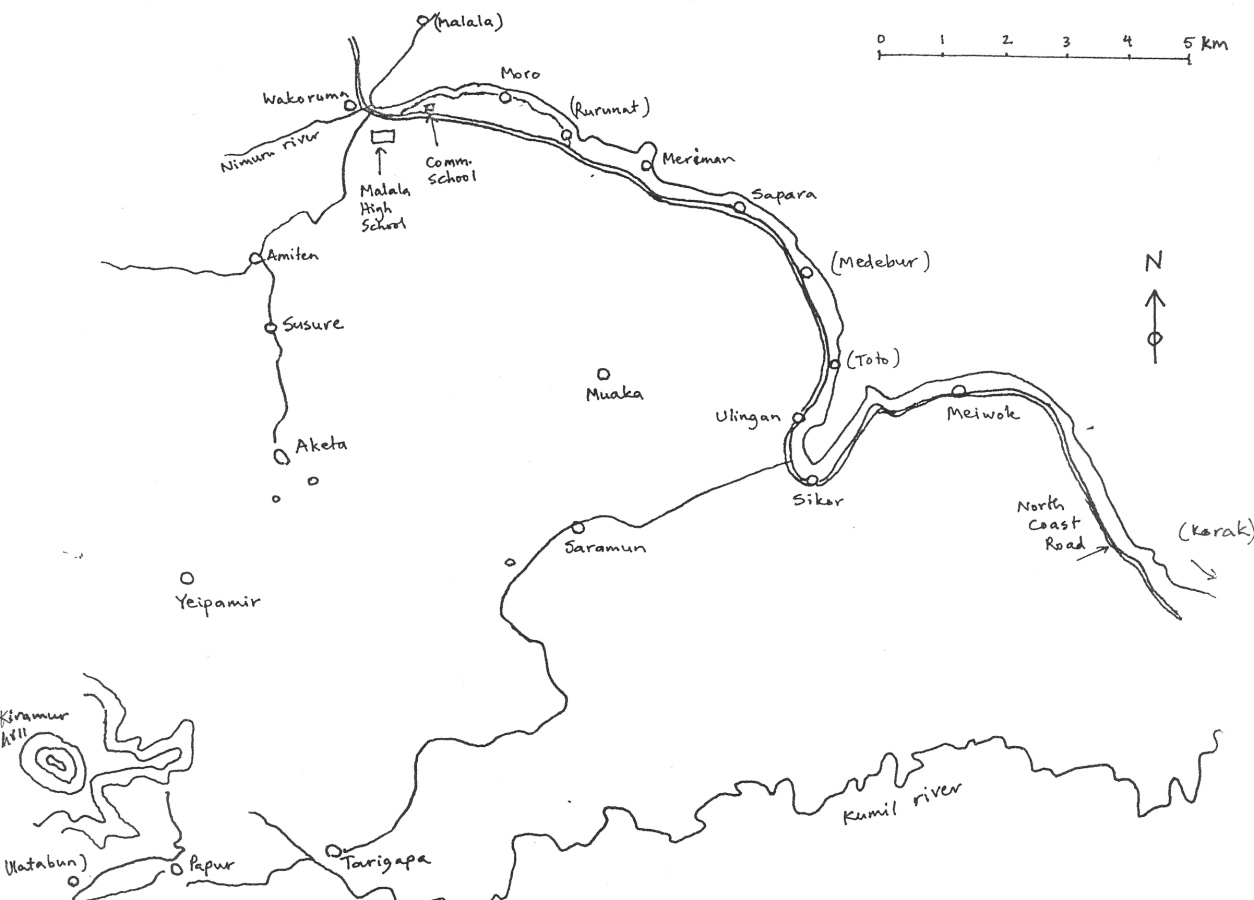
\includegraphics[width=\textwidth]{figures/1-mauwake_language_area_map.jpeg}
\end{figure}

Administratively the Mauwake people belong to the Bogia sub-province and the Almami (derived from the language names Alam--Mauwake--Miani) local level government area. 

There are four primary schools in the area, and one high school.  In all of these schools there are students from more than one language area. The Roman Catholic Church was instrumental in getting the schools started, and is still administering the Malala High School.  Nearly all of the children go to primary school, but the number of Mauwake students in the high school is not very high. Vernacular preschools were started in the whole Mauwake area in the early 1990s, but many of them have since changed into Tok Pisin preschools.

\subsection{On the history of the Mauwake people}
%\hypertarget{RefHeading18461935131865}
Until fairly recently, little was known about the pre-history of the Papuan-speaking people in Near Oceania (including New Guinea island, Bismarck Archipelago and the Solomon Islands), compared with the archaeological information available on the Austro\-ne\-si\-an-speaking people in the area. By the late 1990s it was established that human occupation on the northern coast of New Guinea island dated back to at least 40 000 years. There are signs of semi-domestication of some tree crops from 20 000 to 10 000 years ago, and of agriculture from about 10 000 years ago, roughly the same time that the Highlands valleys became more habitable after the end of the Ice Age \citep[xi--xvii]{Pawley2005a}. 

From the great diversity of the languages around Cape Croisilles area across Karkar Island, \citet[27]{Ross1996} hypothesizes that this probably is where the Croisilles linkage languages, including Mauwake (or its parent language), started spreading from.\footnote{See \sectref{sec:1.4.1} for a description of the genealogical affiliation. }  He does not provide any dates for the migrations.

\largerpage
Besides some traditional myths we have not been able to obtain stories telling about life earlier than the first half of the 20th century.  The majority of the Mauwake people agree that the language group has spread to the coast from inland, and they specify Aketa village as their place of origin. It is commonly believed that long ago the people of the Amiten village, now considered the ``heart area'' of the language by many speakers, spoke a different language, which has since disappeared. \figref{map:1:languagearea} shows the map of Mauwake language area at present. 

The hypothesis that the Mauwake people came from inland would at least partially explain the present language situation on the coast, where there are many languages scattered in a small geographical area. If at some point in history the coast did not have permanent inhabitants to defend it from intruders, it would have been easy for people migrating from various directions and speaking different languages to settle there. One cultural trait that points towards an earlier home area inland is that among the Mauwake speakers fishing is not as important as it is for some other language groups. The coastal villagers mainly catch fish for their own needs, and only occasionally take it to the local market if they happen to have surplus. Gardening, rather than fishing, is the important activity for them.

Possibly the first mention of the larger area where the Mauwake people live is given by the German \citet[338]{Hollrung1888}, who mentions ``the Tsimbin tribe'', meaning the people of Simbine village,\footnote{Situated 8 km from Moro village, and 5 km from the closest Mauwake village.} speaking the Maiani language which borders the Mauwake language area. \citet[964]{Hoeltker1937} calls Maiani and the related languages by the name ``M\'oando languages'' based on the word `man' in those languages.  He also mentions Mauwake as ``Moro--Sapara--Ulingan'' -- picking names of three coastal villages -- as a language deviating from the M\'oando languages (ibid.). 

The written history of the Mauwake area itself began during the German colonial era (ca.~1884--1921) with the report of the killing of two Lutheran missionaries\footnote{The Rhenish Mission had planned to start the work in the area for some time, but it was blocked by the Neu-Guinea-Compagnie. The reason for the killing of the two missionaries, Wilhelm Scheidt and Friedrich Bösch, was never found out, but it is likely that the local people associated them with the Compagnie and feared that they were in fact planters coming to start plantations in their area \citep[106--107]{WagnerEtAl1986}} and an officer of the Neu-Guinea-Compagnie,\footnote{The company had established a big coconut plantation further northwest on an island off Hatzfeldthafen in 1885. It developed quickly despite  various problems, but had to be abandoned completely in 1891 because of the hostility of the inhabitants of the area. Within 20 years the site was again covered by rainforest \citep[450--51]{Tranel1952}.} as well as 14 accompanying native people, in Malala Bay in May 1891 (\citealt[454]{Tranel1952}, \citealt[106--109]{WagnerEtAl1986}).  After this the Lutheran church abandoned the plan to establish a mission station in the area, and founded one further southeast in the Bunabun area instead.

The Roman Catholic mission was then given the authority in 1891 to search the area between Ulingan and Bogia for suitable places for the mission \citep[8]{Duamba1996}.  The Ulingan-Sapara mission station was established in 1926, and a church big enough for a thousand people was built in Sapara village the same year \citep[21]{BrummEtAl1995}%Mihalic
.  A tsunami struck the coast in the morning of Christmas Eve, 1930, killing five people and destroying the new church and the priest's house.\footnote{Presumably the rest of the Sapara village was destroyed as well, as the church was probably the strongest building in the whole village.}  The mission station was moved to the Ulingan village and a new church was built on top of a hill there \citep[20--21]{Davies1999}. The Malala church was built in 1958 on land owned by the Moro villagers, and a high school started on the same compound in 1966 \citep[45]{BrummEtAl1995}%Mihalic
. Both the high school and all the community schools in the area were established by the Catholic Church.  Because of the many missionaries engaged in the work there the local people had a fair amount of contact with Westerners.

In the early years the priests were expected to learn the local language and to become familiar with the culture, especially religious beliefs \citep[25]{BrummEtAl1995}%Mihalic
. The liturgy and some preaching were done in Mauwake too, and a few hymns and prayers were composed in it. But whatever written materials there may have been, they were all lost in the Second World War \citep[3--4]{ZGraggen1971}.  And already in the 1930s Tok Pisin had started to replace the local languages as the official language for evangelization in the Catholic Church \citep[179]{BrummEtAl1995}%Mihalic
.  Especially in an area where five different languages are spoken along a 20 km stretch of the road, this is understandable.  

The Second World War had a profound influence on the area.  In December 1942 thousands of Japanese soldiers landed in Madang and Wewak (ibid. 37).  From Wewak the troops marched down towards Madang, and some of them settled in Ulingan.  They required the local men to help build bridges, and asked the people for food.  The women and also many men from the coastal villages fled to inland villages and to the rainforest, because they were scared of the soldiers.  They were suffering from a shortage of food, as they were not able to do their gardening in a normal way.  The Japanese apparently did not commit cruelties, as was the case in some other areas, and the relationship between them and the local people was uneasy but not hostile. When the Allied forces started to bomb the Japanese-occupied areas, the people had to keep hiding even more and were not even able to cook, as they were afraid that the smoke from their cooking fires might attract the pilots' attention and cause the area to be bombed.  A number of bombs were dropped in the Mauwake language area, and a few people died. 

Before the war, the missionaries were almost the only outsiders that the local people met, but during the war they had contact especially with Japanese but also with Allied soldiers.  After the war a number of young men went to work on plantations in different parts of the country or had other employment outside their home area, thus gaining knowledge of the wider world. The founding of Malala High School in 1966 and the completing of the North Coast Highway in the mid-70's further widened the people's horizons.

\subsection{Demography}   \label{sec:1.3.3} 


%\hypertarget{RefHeading18481935131865}


The inhabitants in the 15 Mauwake-speaking villages number about 4000;  the number is based on the census figures in 2000.  Not all of them speak the language, however, as most of the children now learn Tok Pisin as their first language.\footnote{Much of the contents of the sections \sectref{sec:1.3.3}--\sectref{sec:1.3.6} is based on the Mauwake background study written by Kwan Poh San in 1988.} 


The Mauwake speakers are not a uniform group socially or politically. The basic political unit is a village made up of a few clans. There is usually a main village, with some hamlets attached to it.  Recently there has been a tendency towards moving away from the main village and building small hamlets near the family's garden or coconut plot. 
\newpage 

A person's main responsibility is towards one's own family and clan. The basic unit is a nuclear family: parents and their children, either their own or adopted.  The society is patrilineal: kinship is traced through, and the inheritance handed down from, the father. Adoption is widespread and always takes place within extended family, usually the husband's side of the family.  Members of an extended family are expected to assist each other in various ways: providing food at feasts, helping to pay a debt, bride price or some other obligation, and looking after each other in general. The responsibilities towards one's clan are also strong but not quite as strong as to one's extended family.  Traditionally the clans used to own all the land, but planting coconuts, and later cocoa, changed the situation.  The use of garden land is still decided by the headmen (leaders) of each clan, but now there is rivalry even between members of the same clan about the existing coconut trees and about land where new coconut or cocoa trees can be planted.

Every clan has its own headman, and in earlier times the headman of the most prestigious clan also used to be the headman of the whole village. Decisions were based on consensus after discussions in the village meetings, but the final authority rested on the headmen.

\largerpage
After the establishment of the local level government system the authority of the headmen partly transferred to the local government member (\textstyleForeignWords{kaunsil}), to the magistrate and to the leader of the community work (\textstyleForeignWords{komiti}). The traditional authority structure has more or less broken down and since it has not been completely replaced by the new structure, this has given way to individualism and even disregard of any authority, especially among the young people. The Catholic Church is a somewhat cohesive force, but it has lost some of its authority with the social breakdown and also with the coming of other churches.

Each village has social ties with other, usually closely situated villages regardless of the language.  Many of the Mauwake villages have close interaction with non-Mauwake-speaking villages.  This has also resulted in extensive intermarrying between different language groups, which in the earlier times encouraged bilingualism or trilingualism, but which nowadays strengthens the use of Tok Pisin.

The six languages either bordering the Mauwake area, or inside it, are the Kaukombar\footnote{I am utilizing the grouping from \citet{Ross2005} here. For a discussion on the classification of the Madang languages, see \sectref{sec:1.4.1} below.} languages Maiani, Miani (Tani)\footnote{The names without parentheses are what the speakers prefer to use for their languages, the ones in parentheses are those used in linguistic literature especially by Z'Graggen and those utilizing his data. Maiani and Miani are mentioned here as separate languages, but they can also be considered different dialects of one language.}  and Mala (Pay),\footnote{Mala has two distinct dialects, Mala and Alam. The latter is spoken in the two villages that have close contact with the Mauwake area.} the Tibor language Mawak, the Korak-Waskia group language Amako (Korak), all of which are Trans New Guinea languages; the only Austronesian language is Beteka (Medebur), closely related to the Manam language. None of these languages is dominant compared with the others.  The Mauwake speakers say that it used to be a prestigious language in the area, but I have not been able to confirm this with speakers of the other languages. Bi- and trilingualism used to be extensive in the whole area especially before the arrival of Tok Pisin. 


\subsection{Economy}
%\hypertarget{RefHeading18501935131865}
Subsistence farming is the main activity of the Mauwake people. They get most of their food and building materials from their own land.  Traditionally the main staple was taro, supplemented with yam, sweet potato and cooking bananas; sago was used particularly when little other food was available. Especially on the coast yam and sweet potato have recently been replacing taro as the main staple, because there is not enough land for slash-and-burn gardening required by taro. 

For a long time coconut has been the main cash crop, but with the falling copra prices the people have diversified into growing cocoa, coffee\footnote{Growing coffee was given up later, because it is very labour-intensive and the \textstyleForeignWords{robusta} coffee grown in the lowlands fetches a very low market price.} and recently also vanilla.  The cash crops are transported to Madang to sell.  During the German colonial era tobacco was introduced in the area, and still in the 1930s Malala area was famous for its tobacco \citep[454]{Tranel1952}. Nowadays the people mainly grow it for their own use, and sell any extra at the local market.

Hunting and fishing used to be important activities especially for men, but their significance has decreased. Wild pigs are getting scarce, and bandicoots are mainly hunted during the dry season.  As the Mauwake people have probably come from further inland, fishing has not been as important for them as for some other groups on the coast.  Both men and women do some fishing, but mainly for their own family's needs. 

Any garden produce, fish or bandicoots not needed by the family may be sold at the Malala market, which is the biggest one between Madang and Bogia, or at the smaller Ulingan market.  

The high school and a logging company provide employment for a few local men.  In the area where logging is done landowners also get some royalties from it.  Logging has caused controversy among the people.\footnote{The first logging company in the 1980s went bankrupt and the landowners received very little money for their timber.  Even with subsequent logging the benefits for the local people have been rather modest.} Many of the more educated men, and some women, now in their 40s and 50s, have migrated into towns where they work as tradesmen, teachers, or in other occupations. 

\subsection{Cultural notes} 
%\hypertarget{RefHeading18521935131865}
In the traditional worldview the seen and the unseen are both important parts of the same universe.  The unseen world consists of different kinds of spirits: clan spirits and other spirits in nature (\textstyleStyleVernacularWordsItalic{inasina}), spirits of the recently dead (\textstyleStyleVernacularWordsItalic{kukusa}) and spirits of those who have died a long time ago (\textstyleStyleVernacularWordsItalic{sawur}). The spirits need to be treated with respect so that they will not harm but rather help the people.  Although the reliance on the spirits has decreased with the coming of Christianity, various rituals are still fairly widely practised to ensure the benevolence of the spirits, especially in connection with birth, death, sickness, hunting and gardening. 

\largerpage
Sickness is normally attributed to one's bad relations with other people or disregard of the spirits, the work of a sorcerer, or in some cases to ``natural causes''. Death is still commonly believed to be caused by sorcery.

Name taboos are a typical feature of the cultures in Oceania.  It is forbidden to call one's in-laws by name, or call anyone else by name who has the same name as the in-laws.  In the Mauwake culture both of the parents give a child the name of one of his or her own relatives, which the other parent naturally may not pronounce.  In addition to these two names, a child also receives a Christian name at baptism, and may be given other names as well.  Thus a person can have even five or six names, which are used by different people to call him or her.  And when the person gets married, all those names are forbidden for the in-laws to use.  They may use a kinship term or invent a nickname by which to address the person. In general, kinship terms are used widely both to address people and to refer to them.

Passing on the traditional culture and customs is hampered by the lessening use of the vernacular as well as the lack of interest especially among many young people. Grown-ups may deplore the situation, but there is little attempt to actively pass on the cultural heritage or to help the young generation to evaluate, appreciate and renew their own culture. 





% Key to above graph. Moved to figures/1-mauwake_kinship_system_chart.tex

%\begin{table}
%\begin{tabular}{llllll}
%
%
%\lsptoprule
%
%Ego 	& Subject of chart (male) &&&& 		\\		
%GrFa	& grandfather							& kae & 	Br &	brother 	& yomokowa\\
%GrMo	& grandmother							& kome &	Z &		sister		& ekera\\
%Fr		&	father									&	auwa &	Co &	cousin		& yomar\\
%Mo		&	mother									& aite &	So &	son				& muuka\\
%Un		&	uncle										& yaaya & Da &	daughter	& wiipa\\
%Au		&	aunt										& paapan& Ne &	nephew/nice&eremena\\
%
%\lspbottomrule
%
%\end{tabular}
%\end{table}



\subsection{Mauwake kinship system} \label{sec:1.3.6}
 
%\hypertarget{RefHeading18541935131865}
The kinship system of the Mauwake people is a slightly modified Iroquois system (\figref{fig:1:kinship}). Both gender (of the relative, and in some cases of ego) and generation are important, but also the distinction of parental siblings of the opposite sex. One's father's brother is also called \textstyleStyleVernacularWordsItalic{auwa} `father' and his wife is \textstyleStyleVernacularWordsItalic{aite} `mother'; likewise one's mother's sister is also `mother' and her husband is `father'. But mother's brother is called \textstyleStyleVernacularWordsItalic{yaaya} `uncle', and his wife is \textstyleStyleVernacularWordsItalic{paapan} `aunt'; father's sister is also `aunt' and her husband is `uncle'. The term `father' is used for the following as well: one's own father's cross-cousins, one's father-in law and, for a female, elder sister's husband. Two generations up from self the grandparents are distinguished by gender: \textstyleStyleVernacularWordsItalic{kae} `grandfather' and \textstyleStyleVernacularWordsItalic{kome} `grandmother', but two generations down all the grandchildren are called \textstyleStyleVernacularWordsItalic{iimasip} `grandchild'. 

In one's own generation there are two sets of terms for brothers and sisters. Their use  depends on whether relative age or gender is in focus: \textstyleStyleVernacularWordsItalic{paapa} `older sibling' and \textstyleStyleVernacularWordsItalic{aamun} `younger sibling' are used for siblings of either sex, whereas \textstyleStyleVernacularWordsItalic{yomokowa} `brother'  and \textstyleStyleVernacularWordsItalic{ekera} `sister' are gender-bound terms. The latter are more commonly used by siblings of the opposite sex than by those of the same sex. All the parallel cousins are also considered one's siblings, whereas one's cross-cousins, the children of the `uncles' and `aunts', are called \textstyleStyleVernacularWordsItalic{yomar/emar} `cousin', a term used for either sex.

One generation down from self, one's children include not only one's own sons (\textstyleStyleVernacularWordsItalic{muuka}) and daughters (\textstyleStyleVernacularWordsItalic{wiipa}), but also those of one's siblings of the same sex, \textit{and} those of one's cross-cousins. For the sons and daughters of one's siblings of the opposite sex there is a single term, \textstyleStyleVernacularWordsItalic{eremena} `nephew/niece'. Most of the terms for kin relations are inalienably possessed nouns (\sectref{sec:3.2.4}). 

Mother's brother is a particularly important relative for performing rites of passage like initiation, marriage and funeral. When a person dies, his/her maternal uncle, together with the deceased person's male cross-cousins, is responsible for burying him/her and distributing his/her possessions.\footnote{For an older person whose uncles have already died, nephews (= sons of the siblings of opposite sex) take their place among these men.} These men are called \textstyleStyleVernacularWordsItalic{weria} men.  \textit{Weria} means `planting stick', and the term is used as a metaphor for burial.\footnote{It is not unusual to have the same verb for `burying' and `planting' in Papuan languages, but in Mauwake they are different.} An uncle also has an important function as a mediator, if his nephew or niece has serious problems with his/her nuclear family. Although father's sister's husband is also called an `uncle', he does not have a similar role to that of mother's brother.  


\begin{figure}[h]
%1-mauwake_kinship_system_cart.tex
\resizebox{\textwidth}{!}{
\begin{tikzpicture}

%	Naming Convention for this Picture
%	-------------------------------------
%	Text nodes are in normal letters
%	Shape notes are in ALLCAPS
%
%	Nodes are named 1-n depending on the distance to Ego 
%	Those left of Ego are preceeded by n, those right of Ego are followed by their indexical n

%	Margin conventions
%	Horizontally: Within children of the same parents: 1cm
%		-"-		  Within children of diff. parents: 1.75cm
%
%	Vertically:   Within children of diff. parents: 3.5cm

%Padding for family members
[every rectangle node/.style={inner sep=6pt}]
%circle size, globally
% [every circle node/.sytle={minimum size=.6cm}] Doesn't work, why?

%Ego
\node at (0,0) [rectangle, draw] (ego) {Ego};
\node [above=.1cm of ego,regular polygon, regular polygon sides=3, draw, fill=gray] (EGO) {}; 
%Brother of Ego
\node [left=3cm of ego, rectangle, draw] (1br) {Br};
\node [above=.1cm of 1br, regular polygon, regular polygon sides=3, draw] (1BR) {};
%Sister of Ego
\node [right=3cm of ego, rectangle, draw] (z1) {Z};
\node [above=.1cm of z1, circle, minimum size=.6cm, draw] (Z1) {};

% Ego's cousins on their mother's side
\node [right=1.75cm of z1, rectangle, draw] (br1) {Br};
\node [above=.1cm of br1, regular polygon, regular polygon sides=3, draw] (BR1) {};
\node [right=1cm of br1, rectangle, draw] (z2) {Z};
\node [above=.1cm of z2, circle, minimum size=.6cm, draw] (Z2) {};

\node [right=1.75cm of z2, rectangle, draw] (co1) {Co};
\node [above=.1cm of co1, regular polygon, regular polygon sides=3, draw] (CO1) {};
\node [right=1cm of co1, rectangle, draw] (co2) {Co};
\node [above=.1cm of co2, circle, minimum size=.6cm, draw] (CO2) {};

% Ego's cousins on their mother's side
\node [left=1.75cm of 1br, rectangle, draw] (1z) {Z};
\node [above=.1cm of 1z, circle, minimum size=.6cm, draw] (1Z) {};
\node [left=1cm of 1z, rectangle, draw] (2br) {Br};
\node [above=.1cm of 2br, regular polygon, regular polygon sides=3, draw] (2BR) {};

\node [left=1.75cm of 2br, rectangle, draw] (1co) {Co};
\node [above=.1cm of 1co, circle, minimum size=.6cm, draw] (1CO) {};
\node [left=1cm of 1co, rectangle, draw] (2co) {Co};
\node [above=.1cm of 2co, regular polygon, regular polygon sides=3, draw] (2CO) {};

% Ego's parents
\node [above left=3.5cm and .5cm of ego, rectangle, draw] (1fr) {Fr};
\node [above=.1cm of 1fr, regular polygon, regular polygon sides=3, draw] (1FR) {};
\node [above right=3.5cm and .5cm of ego, rectangle, draw] (mo1) {Mo};
\node [above=.1cm of mo1, circle, minimum size=.6cm, draw] (MO1) {};

% Marriage smyol of Ego's parents
\node [above=3.5cm of EGO] (1frmo1) {\huge{=}};

% Ego's Aunties and Uncles
\node [above=3.5cm of br1, rectangle, draw] (fr1) {Fr};
\node [above=.1cm of fr1, regular polygon, regular polygon sides=3, draw] (FR1) {};
\node [right=1cm of fr1, rectangle, draw] (mo2) {Mo};
\node [above=.1cm of mo2, circle, minimum size=.6cm, draw] (MO2) {};
\node at ($(MO2) !.5! (FR1)$) (fr1mo2) {\huge{=}};

\node [above=3.5cm of co1, rectangle, draw] (un1) {Un};
\node [above=.1cm of un1, regular polygon, regular polygon sides=3, draw] (UN1) {};
\node [right=1cm of un1, rectangle, draw] (au1) {Au};
\node [above=.1cm of au1, circle, minimum size=.6cm, draw] (AU1) {};
\node at ($(UN1) !.5! (AU1)$) (un1au1) {\huge{=}};

\node [above=3.5cm of 2br, rectangle, draw] (2fr) {Fr};
\node [above=.1cm of 2fr, regular polygon, regular polygon sides=3, draw] (2FR) {};
\node [right=1cm of 2fr, rectangle, draw] (1mo) {Mo};
\node [above=.1cm of 1mo, circle, minimum size=.6cm, draw] (1MO) {};
\node at ($(2FR) !.5! (1MO)$) (2fr1mo) {\huge{=}};

\node [above=3.5cm of 2co, rectangle, draw] (1un) {Un};
\node [above=.1cm of 1un, regular polygon, regular polygon sides=3, draw] (1UN) {};
\node [right=1cm of 1un, rectangle, draw] (1au) {Au};
\node [above=.1cm of 1au, circle, minimum size=.6cm, draw] (1AU) {};
\node at ($(1UN) !.5! (1AU)$) (1un1au) {\huge{=}};

% Ego's Grandparents
% ... on their father's side
\node [above=3.5cm of 2fr, rectangle, draw] (1grfa) {GrFa};
\node [above=.1cm of 1grfa, regular polygon, regular polygon sides=3, draw] (1GRFA) {};
\node [right=1cm of 1grfa, rectangle, draw] (1grmo) {GrMo};
\node [above=.1cm of 1grmo, circle, minimum size=.6cm, draw] (1GRMO) {};
\node at ($(1GRFA) !.5! (1GRMO)$) (1grfa1grmo) {\huge{=}};

% ... on their mother's side
\node [above=3.5cm of fr1, rectangle, draw] (grfa1) {GrFa};
\node [above=.1cm of grfa1, regular polygon, regular polygon sides=3, draw] (GRFA1) {};
\node [right=1cm of grfa1, rectangle, draw] (grmo1) {GrMo};
\node [above=.1cm of grmo1, circle, minimum size=.6cm, draw] (GRMO1) {};
\node at ($(GRFA1) !.5! (GRMO1)$) (grfa1grmo1) {\huge{=}};

% Ego's children
\node [below left=3.5cm and .5cm of ego, regular polygon, regular polygon sides=3, draw] (1SO) {};
\node [below=.1cm of 1SO, rectangle, draw] (1so) {So};
\node [right=1cm of 1so, rectangle, draw] (da1) {Da};
\node [above=.1cm of da1, circle, minimum size=.6cm, draw] (DA1) {};

% Ego's Nephews and Niece
\node [left=1.75cm of 1so, rectangle, draw] (1da) {Da};
\node [above=.1cm of 1da, circle, minimum size=.6cm, draw] (1DA) {};
\node [left=1cm of 1da, rectangle, draw] (2so) {So};
\node [above=.1cm of 2so, regular polygon, regular polygon sides=3, draw] (2SO) {};

\node [right=1.75cm of da1, rectangle, draw] (ne1) {Ne};
\node [above=.1cm of ne1, regular polygon, regular polygon sides=3, draw] (NE1) {};
\node [right=1cm of ne1, rectangle, draw] (ne2) {Ne};
\node [above=.1cm of ne2, circle, minimum size=.6cm, draw] (NE2) {};

% Ego's female Cousin's children 

\node [below left=3.5cm and .5cm of 1co, regular polygon, regular polygon sides=3, draw] (3SO) {};
\node [below=.1cm of 3SO, rectangle, draw] (3so) {So};
\node [right=1cm of 3so, rectangle, draw] (2da) {Da};
\node [above=.1cm of 2da, circle, minimum size=.6cm, draw] (2DA) {};


% In-Generation Connections

% Usage of in-generation connections:
% We are using Node Coordinate System, see Section 13.2.3 of the PGF manual
% \draw (node cs:name=NAME, anchor=north) |- +(0,.5) -| (node cs:name=2ndNAME);
% note: We use anchor=north in order to prevent PGF from choosing any other, just in case. We will probably not need it in the second node, though
% note 2: +(0,.5) is a relative position, meaning .5 vertical positive change
% |- means: Go vertical first and then horizontally

% Ego & their immediate Br & Z
\draw (node cs:name=EGO, anchor=north) |- +(0,.5) -| (node cs:name=Z1);
\draw (node cs:name=EGO, anchor=north) |- +(0,.5) -| (node cs:name=1BR);

% Ego's cousins on their mother's side
\draw (node cs:name=BR1, anchor=north) |- +(0,.5) -| (node cs:name=Z2) node [pos=.25] (MBR1Z2) {};
\draw (node cs:name=CO1, anchor=north) |- +(0,.5) -| (node cs:name=CO2) node [pos=.25] (MCO1CO2) {};

% Ego's cousins on their father's side
\draw (node cs:name=1Z, anchor=north) |- +(0,.5) -| (node cs:name=2BR) node [pos=.25] (M1Z2BR) {};
\draw (node cs:name=1CO, anchor=north) |- +(0,.5) -| (node cs:name=2CO) node [pos=.25] (M1CO2CO) {};

% Ego's fathers and his brother and sister
\draw (node cs:name=1FR, anchor=north) |- +(0,.5) -| (node cs:name=1AU);
\draw (node cs:name=1FR, anchor=north) |- +(0,.5) -| (node cs:name=2FR) node [pos=.25] (M1FR2FR) {};

% Ego's mother and her brother and sister
\draw (node cs:name=UN1, anchor=north) |- +(0,.5) -| (node cs:name=MO2);
\draw (node cs:name=UN1, anchor=north) |- +(0,.5) -| (node cs:name=MO1) node [pos=.25] (MUN1NO1) {};

% Ego's children and nephews/nieces
\draw (node cs:name=1SO, anchor=north) |- +(0,.5) -| (node cs:name=DA1) node [pos=.25] (M1SODA1) {};
\draw (node cs:name=NE1, anchor=north) |- +(0,.5) -| (node cs:name=NE2) node [pos=.25] (MNE1NE2) {}; % relative positioning. Not sure why it's 1/4, tough. 
\draw (node cs:name=2SO, anchor=north) |- +(0,.5) -| (node cs:name=1DA) node [pos=.25] (M2SO1DA) {};
\draw (node cs:name=3SO, anchor=north) |- +(0,.5) -| (node cs:name=2DA) node [pos=.25] (M3SO2DA) {};


% Between-Generation Connections

% The old way was \draw (node cs:name=grfa1grmo1, anchor=south) -- ($(grfa1grmo1)-(0,3.225)$); This was extremly messy.
% The new way is to use |- and a seperate node on the |--| specified above. A little tricky, but it should be reliable.


\draw (node cs:name=1frmo1, anchor=south) -- (node cs:name=EGO, anchor=north);
\draw (node cs:name=fr1mo2, anchor=south) |- (node cs:name=MBR1Z2, anchor=center);
\draw (node cs:name=un1au1, anchor=south) |- (node cs:name=MCO1CO2, anchor=center);
\draw (node cs:name=2fr1mo, anchor=south) |- (node cs:name=M1Z2BR, anchor=center);
\draw (node cs:name=1un1au, anchor=south) |- (node cs:name=M1CO2CO, anchor=center);
\draw (node cs:name=grfa1grmo1, anchor=south) |- (node cs:name=MUN1NO1, anchor=center);
\draw (node cs:name=1grfa1grmo, anchor=south) |- (node cs:name=M1FR2FR, anchor=center);
\draw (node cs:name=1co, anchor=south) |- (node cs:name=M3SO2DA, anchor=center);
\draw (node cs:name=ego, anchor=south) |- (node cs:name=M1SODA1, anchor=center);

\draw (node cs:name=1br, anchor=south) |- (node cs:name=M2SO1DA, anchor=center); %This is precise
\draw (node cs:name=z1, anchor=south) |- (node cs:name=MNE1NE2, anchor=center); %This is precise


\end{tikzpicture}}

\vspace{\baselineskip}

\begin{centering}
\begin{tabular}{llllll}
	
	
	\lsptoprule
	
	Ego 	& \multicolumn{2}{l}{Subject of chart (male)} &&& 		\\		
	GrFa	& grandfather	& {\itshape kae} & 	Br &	brother 	& {\itshape yomokowa}\\
	GrMo	& grandmother	& {\itshape kome} &	Z &		sister		& {\itshape ekera}\\
	Fr		&	father		& {\itshape auwa} &	Co &	cousin		& {\itshape yomar}\\
	Mo		&	mother		& {\itshape aite} &	So &	son			& {\itshape muuka}\\
	Un		&	uncle		& {\itshape yaaya} & Da &	daughter	& {\itshape wiipa}\\
	Au		&	aunt		& {\itshape paapan} & Ne &	nephew/nice & {\itshape eremena}\\
	
	\lspbottomrule
	
\end{tabular}
\end{centering}
\caption{Mauwake kinship system chart}
\label{fig:1:kinship}
\end{figure}

\section{The Mauwake language}
%\hypertarget{RefHeading18561935131865}
\subsection{Genealogical affiliation and previous research}\label{sec:1.4.1}
%\hypertarget{RefHeading18581935131865}
The name \emphs{Mauwake} means `what?'\footnote{Actually it consists of the question word \textit{mauwa} `what' and the contrastive focus clitic -\textit{ke}.}  The Mauwake speakers themselves identify the language by this name, and the speakers of the related Kaukombaran languages use corresponding names to call their own languages.  The people have a myth in which the spirit Turamun gives each group their land area, their main staple as well as their language, and the language name originates in this myth.

Before our taking residence in Moro village in 1978, there was only very sketchy research done on the Mauwake language, just enough to classify it.\footnote{\citet{Capell1952}, and following him \citet{VoegelinEtAl1965}, \citet{Greenberg1971}, then \citet{ZGraggen1971,ZGraggen1975a} and \citet{Wurm1975,Wurm1982}.} The name Ulingan was taken from the main mission station in the area, although that is not how the speakers themselves call their language. Sometimes the alternative name Mawake is given in brackets in the earlier language lists.  

Mauwake is a Papuan language. ``Papuan'' is just a cover term for a number of genetically unrelated language families, which are not Austronesian and are spoken in the New Guinea region
(\figref{map:2:NewGuineamap}).\footnote{The name Papuan has been criticized (\citealt{Capell1969}, \citealt{Haiman1979}), but it is widely used instead of its alternative, non-Austronesian.} The Papuan languages consist of several unrelated language families, the biggest of which is the Trans New Guinea (\textsc{tng}) family.  

\begin{figure}[H]
\caption{New Guinea island language map \citep[34 Map~2]{Ross2005}}
\label{map:2:NewGuineamap}
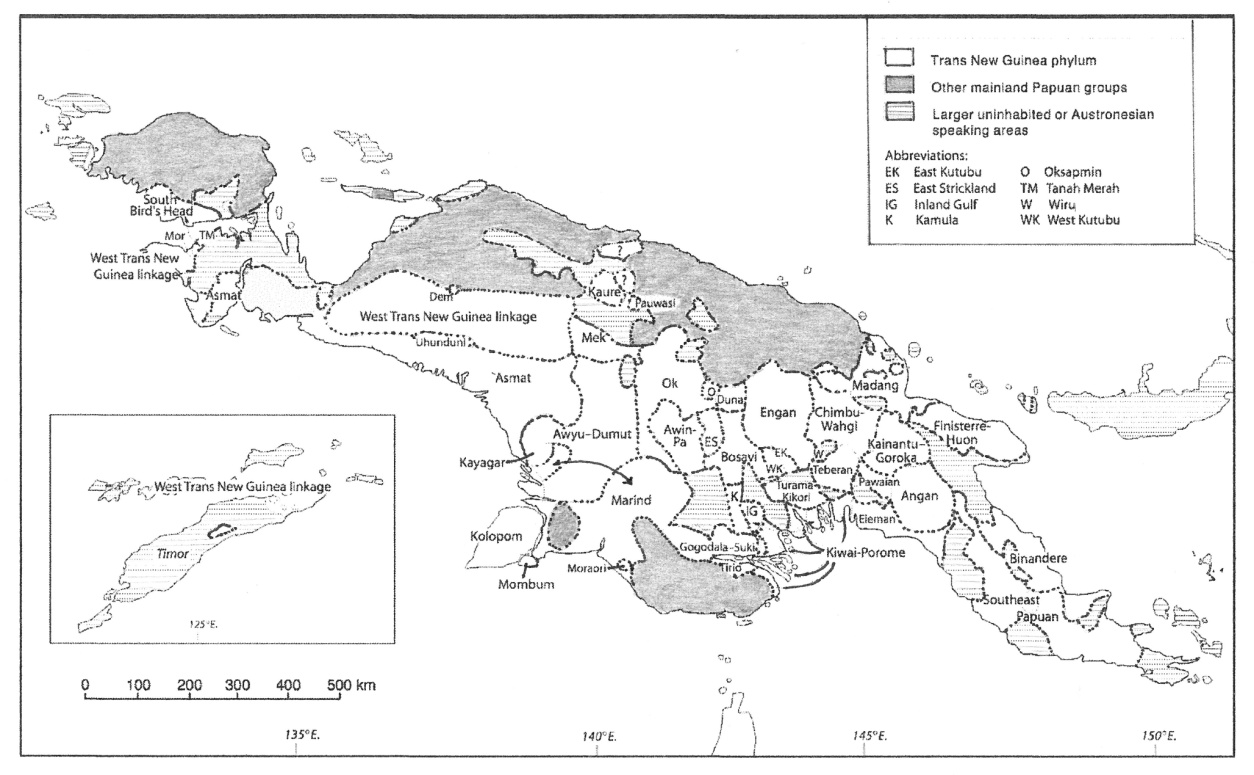
\includegraphics[width=\textwidth]{figures/1-new_guinea_island_language_map.jpeg}
\end{figure}

The Trans New Guinea hypothesis was originally put forward by \citet{McElhanonEtAL1970} to account for the similarities between the Finisterre-Huon languages on the one hand, and Central and South New Guinea Stock languages on the other. Later, \citet{Wurm1975} argued that a great number of additional languages belong to the phylum.  Much of the work relied on lexico-statistical rather than more rigorous application of the standard comparative method, and because many of the claims are not well substantiated, the whole \textsc{tng} hypothesis received a fair bit of criticism (\citealt{Lang1976}, \citealt{Haiman1979}, \citealt{Foley1986}, \citealt{Pawley1995}).

Most of the classificatory work done on the languages of Madang Province is based on groundbreaking research by \citet{ZGraggen1971,ZGraggen1975a,ZGraggen1975b}.  According to \citegen{Wurm1975} classification following the language family tree model of lexicostatistics, Mauwake\footnote{In \citegen{ZGraggen1980} listing Mauwake has the code F2.} belongs to the Madang-Adelbert Range sub-family, Adelbert Range superstock, Pihom stock, and Kumilan\footnote{\citet{ZGraggen1971} initially called the family Ubean, possibly based on the language names Ulingan and Bepour, but later (1975) changed the name into Kumilan based on the name of the Kumil river.} language family together with two very small languages, Bepour and Moere (\figref{map:3:MadangWurm}). 

For nearly two decades there was practically no comparative linguistics done on Pa\-pu\-an languages.  But in the early 1990s more detailed research started on the Madang-Adelbert Range languages, now renamed the Madang group, and later on other \textsc{tng} languages as well \citep{Pawley1998}. As a result of that research \citet{Pawley1995, Pawley2001} and \citet{Ross1995} came to the conclusion that the Trans New Guinea hypothesis is workable but needs modification. They also concluded that the Madang group definitely is part of the Trans New Guinea language family. According to their new classification Mauwake belongs to the Trans New Guinea family, the Madang group and the Croisilles linkage of languages. \citet[21--25]{Ross1996} also discusses the relationships between the various languages within the Croisilles subgroup, using the term \textit{Kumil} (Z'Graggen's  \textit{Kumilan}) for the family including Mauwake, and \textit{Kaukombar} (Z'Graggen's \textit{Kaukombaran}) for the four languages closest to the Kumil languages. He also does some regrouping within the families based on the pronoun  forms in the languages.  In the Kumil group he includes not only Mauwake, Bepour and Moere, but also the languages Musar and Bunabun (\figref{map:4:MadangRoss}). 

Apart from Z'Graggen's survey no other linguistic study of any depth has been carried out on the Mauwake language except what has been done by Kwan Poh San and myself (\citealt{Kwan1980, Kwan1983, Kwan1988, Kwan1989, Kwan2002}; \citealt{Jarvinen1980,Jarvinen1988a,Jarvinen1988b,Jarvinen1989,Jarvinen1990,Jarvinen1991}; \citealt{JarvinenEtAl2001}, and \citealt{Berghall2006}.)  The grammatical work published on related languages includes the grammars of Usan by \citet{Reesink1987}, Tauya by \citet{MacDonald1990} and Waskia by \citet{RossEtAl1978}. Two grammars in manuscript form that were also used for reference are Maia grammar by Hardin (\citeyear{Hardin2002}) and Bargam grammar by Hepner (\citeyear{Hepner2002}). Both are available electronically and in the \textsc{sil-png} library, Ukarumpa.

The \textsc{iso}-639 code for Mauwake, based on \citet{Grimes2000}, is mhl, and the Glottolog code is mauw1238 (glottolog.org).

\clearpage
\begin{figure}[p]
	\caption{Wurm's grouping of Madang-Adelbert languages \citep [Map~3]{Ross1996}}
	\label{map:3:MadangWurm}
	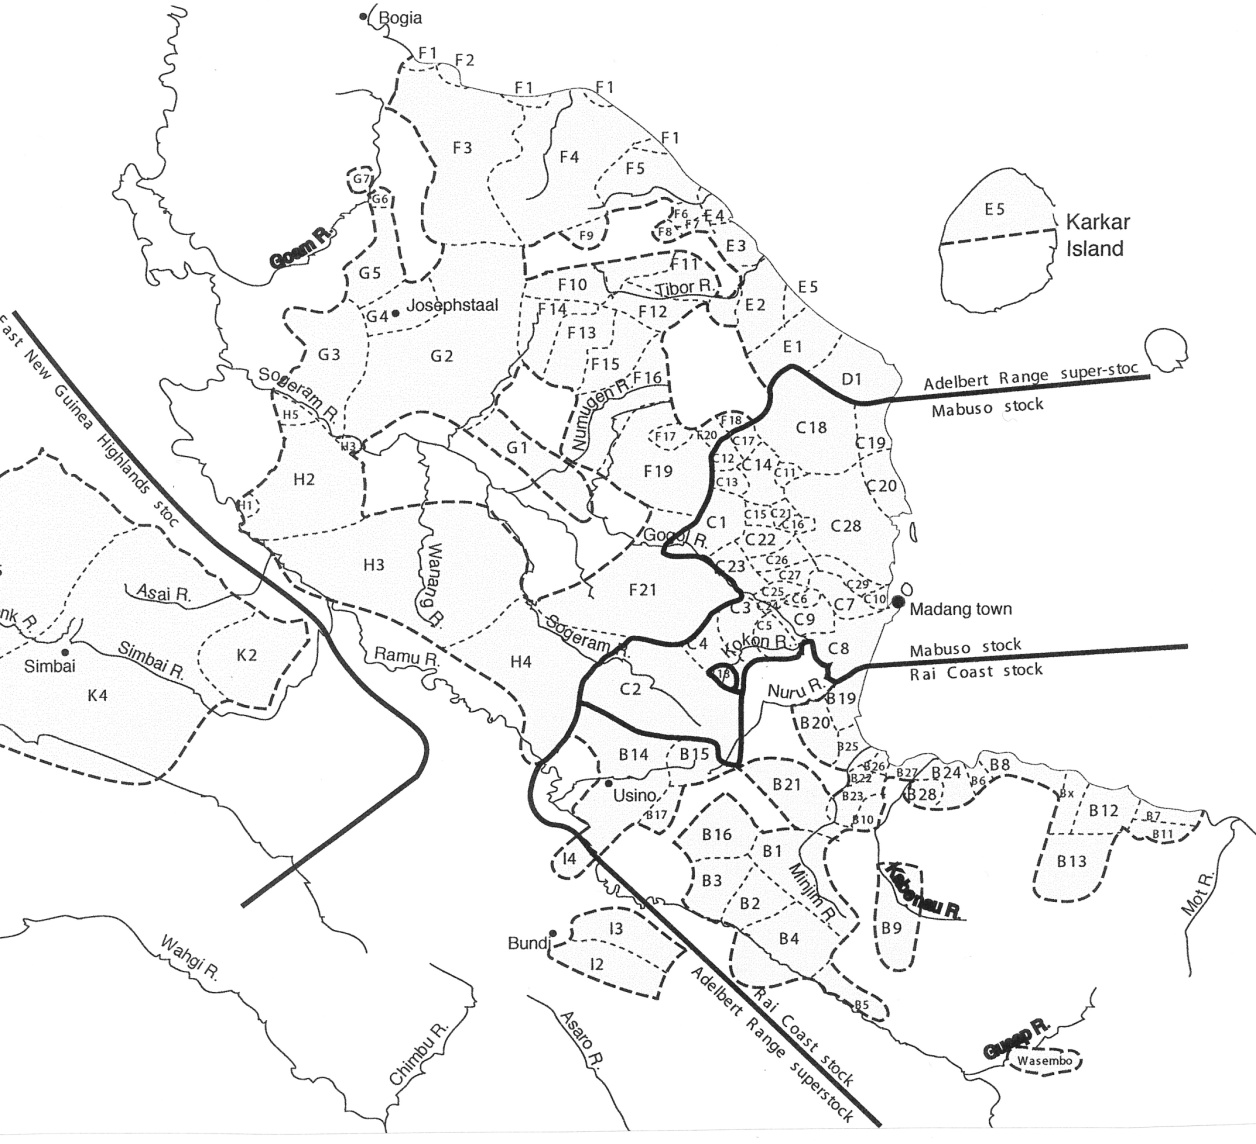
\includegraphics[width=\textwidth]{figures/1-wurms_grouping_of_madang_adelbert_languages.jpeg}
\end{figure}

\clearpage
\begin{figure}
\caption{Ross' 1996 grouping of Madang-Adelbert languages \citep[Map~4]{Ross1996}}
\label{map:4:MadangRoss}
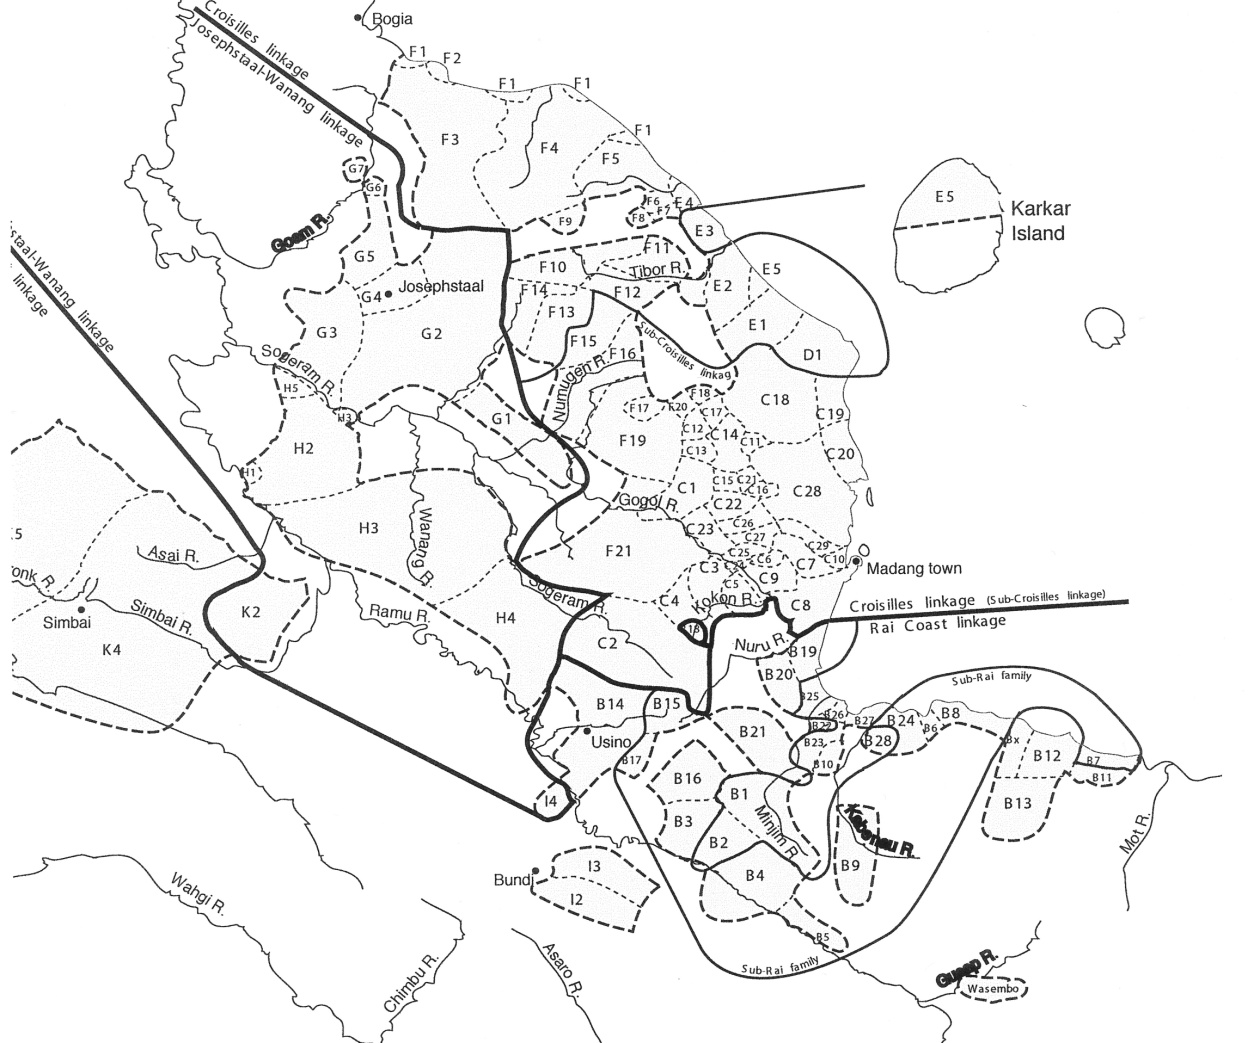
\includegraphics[width=\textwidth]{figures/1-ross_grouping_of_Madang_Adelbert_languages_map.jpeg}
\end{figure}



\subsection{Typological overview of morphological and syntactic features}
%\hypertarget{RefHeading18601935131865}
In this section, morphological and syntactic characteristics of the Mauwake language are discussed in relation to the typology of Papuan/Trans New Guinea languages and to the universal word order\footnote{As \citet[72]{Dixon2010a} notes, ``word order'' here should be called ``the order of clausal constituents'', as it is the ordering of constituents that the typology is based on rather than that of individual words.}  typology.  To some extent these two overlap, as \textsc{tng} languages typically are also \textsc{sov} languages.

\subsubsection{Mauwake as a Trans New Guinea language}
%\hypertarget{RefHeading18621935131865}
Mauwake has many features typical of both Papuan languages in general and Trans New Guinea languages in particular. 

\largerpage
The \textstyleEmphasizedWords{{phonology}} of the language is simple: there are five vowel and fourteen consonant phonemes, and only a few of them have more than one allophone.  Morphology is quite transparent, so there is very little morphophonology.

The \textstyleEmphasizedWords{{basic}} \textstyleEmphasizedWords{{order of clausal constituents}} is verb-final. In neutral clauses with both subject and object the order is \textsc{sov} \REF{ex:1:x656}, but it changes into \textsc{osv} when the object is fronted \REF{ex:1:x657} as a theme (\sectref{sec:9.1}).  Adverbials are somewhat less constrained in their ordering. It is also very common to have a verb as the only element in a clause \REF{ex:1:x659}. 

\ea%x656
\label{ex:1:x656}
\gll {\ob}Ona  emeria  nain=ke{\cb}\textsubscript{S} {\ob}maa{\cb}\textsubscript{O} wafur-a-k. \\
 3s.\textsc{gen} woman  that1=\textsc{cf}  thing  throw-\textsc{pa}-3s \\
\glt `His wife threw things.'
\z


\ea%x657
\label{ex:1:x657}
\gll {\ob}Wiipa  nain{\cb}\textsubscript{O} {\ob}eka=ke{\cb}\textsubscript{S} mu-o-k. \\
 daughter  that1  water=\textsc{cf} swallow-\textsc{pa}-3s     \\
\glt `The daughter was swallowed by the water.'
\z


\ea%x659
\label{ex:1:x659}
\gll Uruf-a-m. \\
 see-\textsc{pa}-1s     \\
\glt `I saw it.'
\z


In \textstyleEmphasizedWords{{complex sentences}}, the subordinate clause usually precedes the main clause.  Thus the reason/cause precedes the result/effect, in conditional sentences the protasis precedes the apodosis, and in intention/purpose sentences the intention precedes the expected result. When the reason follows the result, it is a very marked order.

Mauwake is clearly a nominative-accusative type language, rather than ergative-\linebreak absolutive. The agent of a transitive verb \REF{ex:1:x1523} is marked in the same way as the actor of an intransitive verb \REF{ex:1:x1524}, and most experiential verbs have the experiencer as a nominative subject \REF{ex:1:x1525}.

\ea%x1523
\label{ex:1:x1523}
\gll Yo  mauw-owa  nia  asip-i-yem. \\
 1s.\textsc{unm}  work-\textsc{nmz}  2p.\textsc{acc}  help-\textsc{Np}-\textsc{pr}.1s     \\
\glt `I help you with work.'
\z


\ea%x1524
\label{ex:1:x1524}
\gll Yo  koka=pa  ik-e-m. \\
1s.\textsc{unm}  jungle=\textsc{loc}  be-\textsc{pa}-1s      \\
\glt `I was in the jungle.'
\z


\ea%x1525
\label{ex:1:x1525}
\gll Yo  wuailal-i-yem  a. \\
 1s.\textsc{unm}  hunger-\textsc{Np}-\textsc{pr}.1s  oh     \\
\glt `Oh, I'm hungry.'
\z


\textstyleEmphasizedWords{{Verb morphology}} in Mauwake is extensive, even if not as extensive and complex as in some other Papuan languages. The morphology is agglutinative, and  affixation is mostly very transparent.  Suffixes are used for subject, tense and aspect, benefactive, distributive, causative and counterfactual marking. Prefixing is used very little, only for reduplication and to form verbs referring to bringing and taking. It is possible to have several derivational and inflectional affixes in one verb, as shown by the elicited example \REF{ex:1:x664}, but in actual usage this is rare.


\ea%x664
\label{ex:1:x664}
\gll Muuka  wia \textstyleEmphasizedVernacularWords{arim-ow-omak-om-ek-a-k}. \\
 son  3p.\textsc{acc}  grow-\textsc{caus}-\textsc{distr/pl}-\textsc{ben}-\textsc{bnfy1.\textsc{cntf}-pa}-3s     \\
\glt `(S)he would have brought up (many) sons for me.'
\z


Mauwake has a clear three-tense system (\sectref{sec:3.8.3.4}). Even though the tense suffixes only distinguish between past and non-past, the distinction between present and future shows in the subject suffixes, which are different for these two tenses.  Aspect marking is optional (\sectref{sec:3.8.5.1.1}).  The auxiliary follows the main verb. There is no passive form in verbs.

A very typical feature in Papuan languages is a difference between final (\sectref{sec:3.8.3.4}) and medial verbs (\sectref{sec:3.8.3.5}). The former are finite verbs with full inflection for tense and subject number and person, and the most typical position for them is at the end of a declarative sentence. The medial verbs indicate whether the subject of a clause is the same as \REF{ex:1:x662}, or different from \REF{ex:1:x663}, that of the following clause. The same-subject forms also indicate whether the action of the second verb is simultaneous with that of the first verb, or sequential \REF{ex:1:x662} in relation to it. Medial clauses (\sectref{sec:8.2}) are coordinate with, but also dependent on, the following clause. Because of the existence and extensive use of medial clauses, temporal subordinate clauses (\sectref{sec:8.3.3.1}) are used very little in Mauwake.\footnote{Medial clauses in Papuan languages are often translated with temporal subordinate clauses in other languages, even if they are not subordinate in the original language.}

\ea%x662
\label{ex:1:x662}
\gll Owowa  or-\textstyleEmphasizedVernacularWords{op},  wuailal-\textstyleEmphasizedVernacularWords{ep}  akia  ik-e-k. \\
village  go-\textsc{ss.seq} be.hungry-\textsc{ss.seq} banana  roast-\textsc{pa}-3s      \\
\glt `He went to the village, was hungry and roasted bananas.'
\z

 
\ea%x663
\label{ex:1:x663}
\gll Mik-\textstyleEmphasizedVernacularWords{amkun}   me  um-o-k,  wiowa  onaiya  ikiw-em-ik-\textstyleEmphasizedVernacularWords{eya}. Olas=ke  war-e-k.\\
spear-1s/p.\textsc{ds}  not  die-\textsc{pa}-3s  spear  with  go-\textsc{ss.sim}-be-2/3s.\textsc{ds} Olas=\textsc{cf}  kill-\textsc{pa}-3s\\
\glt`When I speared it, it didn't die, (but) as it was going with the spear Olas killed it.'
\z


Medial verbs are also used in tail-head linkage (\sectref{sec:8.2.3.5}), another strategy common in Papuan languages. The last verb of a sentence is repeated in the first clause of the next sentence, but usually in medial form.  In spoken Mauwake this recapitulation device is used to indicate actions that continue on the story line without a major break, but since the development of the written language the tail-head linkage is losing this function and is getting a new function as a  marker of the climax in the story.

Another typical feature of many Papuan languages is the lack of a large inventory of verb stems \citep[127]{Foley1986}. An extreme case is Kalam with its less than 100 verb stems; consequently, Kalam needs to use serial verb and adjunct plus verb constructions for most actions \citep[336--337]{Pawley1987}. Mauwake has a reasonably large verb inventory, but in addition it uses both serial verbs (\sectref{sec:3.8.5.1.2}) and adjunct plus verb constructions (\sectref{sec:3.8.5.2}).

There is no inflection on \textstyleEmphasizedWords{{nouns}} (\sectref{sec:3.2}) or \textstyleEmphasizedWords{{adjectives}}  (\sectref{sec:3.3}), nor are there gender/noun class distinctions. But Mauwake makes a distinction between alienably and inalienably possessed nouns (\sectref{sec:3.2.4}).  Most kinship terms are inalienably possessed, but body parts are not.

The \textstyleEmphasizedWords{{noun phrase}} (\sectref{sec:4.1}) most commonly consists of the head noun by itself, or with just one modifier.  In a noun phrase a pluralizing \REF{ex:1:x658} unmarked pronoun, a possessive noun phrase, a temporal phrase, or a qualifier noun phrase may precede the head noun; all the other modifiers follow it. A possessive preceding the head noun and an adjective following it \REF{ex:1:x660} is quite common in Trans New Guinea languages \citep[19]{Reesink1987}. 

\ea%x658
\label{ex:1:x658}
\gll \textstyleEmphasizedVernacularWords{wi} \textstyleEmphasizedVernacularWords{emeria}  teeria  nain \\
 3p.\textsc{unm}  woman  group  that1     \\
\glt `that group of women'
\z


\ea%x660
\label{ex:1:x660}
\gll \textstyleEmphasizedVernacularWords{yena}  aamun  \textstyleEmphasizedVernacularWords{gelemuta}  kuisow \\
 1s.\textsc{gen}  1s/p.younger.sibling  small  one     \\
\glt`my one younger brother' or `one of my younger brothers'
\z 


Mauwake exhibits more variation in the \textstyleEmphasizedWords{{pronoun}} forms (\sectref{sec:3.5}) than many other Papuan languages do.  There is only singular and plural number, and no inclusive-exclusive distinction in the first person plural.  But there are separate sets for unmarked, accusative, dative, genitive, isolative, reflexive-reciprocal and comitative pronouns.  Mauwake is a typical Papuan language in that the subject pronoun may be left out; the third person subject pronoun is overt  mainly when it is used for a re-activating an earlier topic (\sectref{sec:9.2.3}).  But in imperative clauses a subject pronoun is very common, which is \textstyleEmphasizedWords{not} usually mentioned as a typical feature of Papuan languages,\footnote{To my knowledge this particular feature has not been studied much in Papuan languages.}  and is quite rare cross-linguistically.

\subsubsection{Mauwake as an \textsc{sov} language} \label{sec:1.4.2.2}
%\hypertarget{RefHeading18641935131865}
Mauwake conforms very strongly to the typological patterns found to exist in the \textsc{sov}, or hence, \textsc{ov} languages.  The following discussion on various characteristics in Mauwake that correlate with the \textsc{ov} constituent order is based on \citet{Dryer2007a}.
 
Concerning the following sentence level features Mauwake shows itself a typical \textsc{ov} language.  The interrogative marker \textstyleStyleVernacularWordsItalic{-i}  always occurs sentence-finally in polar questions \REF{ex:1:x672} (\sectref{sec:7.2.2}).

\ea%x672
\label{ex:1:x672}
\gll Yo  emeria  efar  uruf-a-man=\textstyleEmphasizedVernacularWords{i}? \\
1s.\textsc{unm} woman  1s.\textsc{dat}  see-\textsc{pa}-2p=\textsc{qm}     \\
\glt`Did you see my wife?'
\z


In non-polar, or content questions (\sectref{sec:7.2.1}), the question word or phrase is in the same position that would be occupied by the non-interrogative word or phrase in a statement~\REF{ex:1:x673}.

\ea%x673
\label{ex:1:x673}
\gll Ni  sira \textstyleEmphasizedVernacularWords{kamenap}  on-a-man? \\
2p.\textsc{unm}  custom  what.like  do-\textsc{pa}-2p      \\
\glt`What did you do?'
\z


In complex sentences (\sectref{sec:8.3}), the subordinate clause usually comes before the main clause \REF{ex:1:x674}.

\ea%x674
\label{ex:1:x674}
\gll Mua  imen-ap=\textstyleEmphasizedVernacularWords{na}  feeke  wia  p-ekap-eka. \\
 man  find-\textsc{ss}.\textsc{seq}=\textsc{tp}  here.\textsc{cf}  3p.\textsc{acc}  \textsc{bpx}-come-\textsc{imp}.2p     \\
\glt`If you find the men, bring them here.'
\z


Complement clauses (\sectref{sec:8.3.2}) behave like other subordinate clauses, preceding the main clause \REF{ex:1:x675}. 

\ea%x675
\label{ex:1:x675}
\gll \textstyleEmphasizedVernacularWords{Mukuna}  \textstyleEmphasizedVernacularWords{kerer-e-k}  \textstyleEmphasizedVernacularWords{nain} i  me  paayar-e-mik. \\
fire  start-\textsc{pa}-3s  that1  1p.\textsc{unm}  not  understand-\textsc{pa}-1/3p      \\
\glt`We didn't realise that a fire had started.'
\z


The typical \textsc{ov} order for predicate-copula applies only partly in Mauwake, as a copular verb is not used for for the present tense. The \textsc{ov} order does show in the other tenses and the medial forms \REF{ex:1:x676}.

\ea%x676
\label{ex:1:x676}
\gll O  somek  mua(=pa) \textstyleEmphasizedVernacularWords{ik-eya {\dots}}  \\
3s.\textsc{unm}  song  man-(\textsc{loc})  be-2/3s.\textsc{ds}      \\
\glt`When he was a teacher {\dots}'
\z


Clause and sentence level features that correlate with the \textsc{ov} order are as follows. The position of a complementizer or a subordinator is clause-final \REF{ex:1:x677}.

\ea%x677
\label{ex:1:x677}
\gll Yo  emeria  aaw-owa  kookal-ek-a-m=\textstyleEmphasizedVernacularWords{na  {\dots}} \\
 1s.\textsc{unm}  woman  get-\textsc{nmr}  like-\textsc{cntf}-\textsc{pa}-1s=\textsc{tp} \\
\glt`If I had liked/wanted to get a wife ...  '
\z


Both manner adverbs, postpositional phrases, and non-argument noun phrases precede the verb \REF{ex:1:x678}.

\ea%x678
\label{ex:1:x678}
\gll Fikera  nain \textstyleEmphasizedVernacularWords{sira}  \textstyleEmphasizedVernacularWords{feenap}  on-a-mik. \\
  kunai.grass  that1  custom  like.this  do-\textsc{pa}-1/3p    \\
\glt `This is what they did to the \textstyleForeignWords{kunai} grass.'
\z


Typical \textsc{ov} features also manifest themselves in different phrases. In the \textsc{vp}s (or verbal groups, as they are called below in \sectref{sec:3.8.5.1}), the main verb precedes the auxiliary  \REF{ex:1:x679}.

\ea%x679
\label{ex:1:x679}
\gll Saa=iw \textstyleEmphasizedVernacularWords{ir-am-ika-i-mik}. \\
 sand=\textsc{inst} come-\textsc{ss}.\textsc{sim}-be-\textsc{Np}-\textsc{pr}.1/3p \\
\glt`They are coming along the sand/beach.'
\z


In basic noun phrases (\sectref{sec:4.1.1}) the genitive precedes the head noun  \REF{ex:1:x680}:

\ea%x680
\label{ex:1:x680}
\gll yiena miiwa \\
 1p.\textsc{gen} land \\
\glt`our land'
\z


Mauwake does not have articles. When the distal-1 deictic \textstyleStyleVernacularWordsItalic{nain} `that' is used, there is often considerable semantic bleaching, and it seems to be becoming more like a definite article, but in many contexts it still clearly retains its deictic function.

Mauwake has postpositional phrases (\textsc{pp}), rather than prepositional phrases \REF{ex:1:x681}.

\ea%x681
\label{ex:1:x681}
\gll koor(a) kuenuma=pa \\
 house underside=\textsc{loc} \\
\glt`underneath the house'
\z


An \textsc{ov} feature that shows on word level in Mauwake is that verbs have suffixes rather than prefixes \REF{ex:1:x682}.

\ea%x682
\label{ex:1:x682}
\gll Akia  ik-\textstyleEmphasizedVernacularWords{omak-e-mik}. \\
 banana  roast-\textsc{distr}/\textsc{pl}-\textsc{pa}-1/3p     \\
\glt`We roasted many bananas.'
\z


As there are no comparative forms for adjectives in Mauwake, one \textsc{ov} characteristic that does not apply in Mauwake is the standard of comparison and comparison marker preceding the adjective. 

Case marking of transitive arguments with an affix is more common in \textsc{ov} than in \textsc{vo} languages.  In Mauwake there are no case suffixes on either the subject or the object, but all human objects require an accusative pronoun (\sectref{sec:3.5.3}) to occur preceding the verb.

\subsection{Dialects}
%\hypertarget{RefHeading18661935131865}


The Mauwake speakers themselves do not identify clearly defined dialects, but they do refer to the speech differences between the inland villages and the coastal villages.\footnote{The data for this section is mainly taken from the Mauwake dialect survey report \citep{Jarvinen1988b}.} Some also separate the Ulingan group from the rest, and the Ulingan group people make a distinction between themselves and those further west along the coast.

The majority of the Mauwake speakers consider Aketa and Amiten as the centre of the language group. People in each village claim that their own way of speaking is the ``true'' way, but at the same time they credit Aketa as the place where the language originated.  The Ulingan and Papur dialect groups do not admit the prestige of Aketa and Amiten quite as willingly.

Comparing the Mauwake data\footnote{The basic 100-word list by \citet[55--59]{Ezard1977} was used with four semantically problematic words deleted and four other words added.} lexicostatistically would indicate that there are no distinct dialects in the language at all. The percentage of cognates between all the villages is 100.  What variation an earlier survey seemed to show, turned out to be multiple cognates. But the phonostatistic method (\citealt{GrimesEtAl1959}, modified as in \citealt[177--178]{Simons1977}) yields some dialectal differences. There are pronunciation dissimilarities, on the basis of which the language area can be divided into three main dialect areas: Ulingan (Ulingan, Sikor and Meiwok), Papur (Papur, Tarikapa, Yeipamir) and Muaka (Muaka, Moro, Mereman, Sapara, Aketa, Amiten/Susure/Wakoruma,\footnote{Susure and Wakoruma were not included in this survey because of their closeness to Amiten both location- and dialect-wise.} and Saramun). 

Of the 100 words in the list, 60\% are pronounced identically in all the villages.  Of the rest, a little over half (i.e. 21\% of the whole data) are cases of non-phonemic variation, namely [\emphs{w}]{\Tilde}[\emphs{β}], and [\emphs{j}]{\Tilde}[\emphs{{\textyogh}}]. The first one of these the speakers of the language do not even notice, the second one they notice to some extent. 
\figref{map:5:pronunciationdiff} gives the mean degrees\footnote{The mean degree of difference between two sounds was calculated by first counting hypothesized minimal steps from one to another, one minimal step given the value of one. These were added up and divided by the number of words in the data, i.e. 100.} of pronunciation differences between some of the Mauwake villages.

\begin{figure}[t]
\caption{Mean degrees of pronunciation difference between some Mauwake villages}
\label{map:5:pronunciationdiff}
\pgfdeclarelayer{bg}
\pgfdeclarelayer{bg2}
\pgfsetlayers{bg2,bg,main}
\resizebox{\textwidth}{!}{
\begin{tikzpicture}[baseline]


\node	(moro)				at	(0,0)									{Moro};
\node	(meriman)			[below right=9mm and 21mm of moro]			{Meriman};
\node	(sapara)			[below right=6mm and 12mm of meriman]		{Sapara};
\node	(muaka)				[below=20mm of meriman]						{Muaka};
\node	(amiten)			[below left=20mm and 13mm of moro]			{Amiten};	
\node	(aketa)				[below=45mm of moro]		{Aketa};
\node	(saramun)			[right=46.75mm of aketa]						{Saramun};
\node	(yeipamir)			[below right=9mm and 18mm of aketa]			{Yeipamir};
\node	(papur)				[below right=24mm and 0mm of aketa]			{Papur};
\node	(tarigapa)			[right=30mm of papur]						{Tarigapa};
\node	(ulingan)		  	[right=40mm of muaka]						{Ulingan};
\node	(meiwok)			[right=30mm of ulingan]						{Meiwok};
\node	(sikor)				[right=39mm of saramun]		{Sikor};

\node	(susure)			[below=15mm of amiten]						{(Susure)};
\node	(wakoruma)			[below left=8mm and 17mm of moro]			{(Wakoruma)};


% Categories
\begin{pgfonlayer}{bg}
\node (kat1) [fill=gray!15, draw, dashed, rounded corners=15, fit=(moro) (meriman) (sapara) (muaka)] {};
\node (kat2) [fill=gray!15, draw, dashed, rounded corners=15, fit= (ulingan) (sikor) (meiwok)] {};
\node (kat3) [fill=gray!15, draw, dashed, rounded corners=15, fit= (papur) (yeipamir) (tarigapa)] {}; 
\end{pgfonlayer}
\begin{pgfonlayer}{bg2}
\node (kat4) [fill=gray!5,draw, dotted, rounded corners=15, fit = (kat1) (amiten) (aketa) (saramun), inner sep=10pt]{}; 
\end{pgfonlayer}

\footnotesize{
% Moro Relations
\path	(moro)	edge node [sloped, above] {0.04}							(meriman);
\path (moro)	edge [bend left] node [sloped, above] {0.06}	(sapara);
\path (moro)	edge [bend right=10] node [sloped, above] {0.03} (muaka);
\path (moro) 	edge node [sloped, below] {0.07} (aketa);
\path (moro)	edge [bend right] node [sloped, above] {0.09} (amiten); 

% Meriman Relations
\path (meriman) 	edge [sloped, above] node {0.04} (sapara);
\path (meriman) 	edge node [sloped, above] {0.04} (aketa);
\path (meriman) 	edge node [sloped, above, pos=0.333] {0.07} (muaka);

% Sapara Relations
\path (sapara) 	edge [bend right=20] node [sloped, above right] {0.05} (aketa);
\path (sapara) 	edge node [sloped, above] {0.07} (ulingan);
\path (sapara) 	edge node [sloped, below left] {0.05} (saramun);
\path (sapara) 	edge node [sloped, above left] {0.08} (muaka);

% Amiten Relations
\path (amiten)	edge node [sloped, below] {0.07}	(muaka);
\path (amiten)	edge [bend right] node [sloped,below left] {0.09}	(aketa);

% Muaka Relations
\path (muaka)	edge node [sloped, above right] {0.11}	(ulingan);
\path (muaka)	edge node [sloped, below] {0.08}	(saramun);
\path (muaka)	edge node [sloped, above] {0.11}	(tarigapa);
\path (muaka)	edge [bend left=10] node [sloped, below, pos=0.575] {0.10}	(yeipamir);
\path (muaka)	edge node [sloped, below] {0.11}	(aketa);

% Ulingan Relations
\path (ulingan) edge node [sloped, below] {0.12}	(saramun);
\path (ulingan) edge node [sloped, above] {0.15}	(tarigapa);
\path (ulingan) edge node [sloped, above] {0.02}	(sikor);
\path (ulingan) edge node [sloped, above] {0.03}	(meiwok);

% Aketa Relations
\path (aketa) edge node [sloped, below, pos=0.333] {0.08}	(papur);
\path (aketa) edge node [sloped, above] {0.08}	(yeipamir);
\path (aketa) edge node [sloped, below] {0.11}	(saramun);

% Saramun Relations
\path (saramun) edge node [sloped, below] {0.09}	(tarigapa);
\path (saramun) edge [bend left=35] node [above, sloped] {0.14}	(meiwok);
\path (saramun) edge node [sloped, above] {0.13}	(sikor);

% Sikor Relations
\path (sikor) edge node [sloped, above] {0.02}	(meiwok);
\path (sikor) edge node [sloped, below right] {0.14}	(tarigapa);

% Meiwok Relations
\path (meiwok) edge [bend left] node [sloped, below right] {0.17}	(tarigapa);

% Yeipamir Relations
\path (yeipamir) edge node [sloped, above] {0.03} (papur);
\path (yeipamir) edge node [sloped, below] {0.08} (tarigapa);

% Papur Relations
\path (papur) edge node [below] {0.11} 	(tarigapa);

% Tarigapa Relations
% Will be empty for now.
}
\end{tikzpicture}
}
\end{figure}





The Ulingan dialect is the most homogeneous, and also most clearly a separate group from the others. The mean degree of pronunciation differences between Ulingan and Sikor, and between Sikor and Meiwok is 0.02, which means that in a hundred-word list there are only two differences of one degree.  The pronunciation difference between Tarikapa and Sikor or Meiwok is the biggest, 0.17 degrees. 
\tabref{tab:1:pronunciationdiff} gives the mean degrees of pronunciation differences between all the villages.



\begin{table} 
\caption{Mean degrees of pronunciation differences between Mauwake villages}
\label{tab:1:pronunciationdiff}
\begin{tabularx}{\textwidth}{lllllllllllll}

\mytoprule  
\begin{rotate}{0}{Muaka}\end{rotate}\\ 
.08 & \begin{rotate}{0}{Saramun}\end{rotate} &  &  &  &  &  &  &  &  &  &  &  \\

.11 & .09 & \begin{rotate}{0}{Tarikapa}\end{rotate}  &  &  &  &  &  &  &  &  &  &\\

.10 & .12 & .11 & \begin{rotate}{0}{Papur}\end{rotate} &  &  &  &  &  &  &  &  &\\

.10 & .11 & .08 & .03 & \begin{rotate}{0}{Yeipamir}\end{rotate} &  &  &  &  &  &  &  &\\

.07 & .11 & .07 & .08 & .08 & \begin{rotate}{0}{Aketa}\end{rotate} &  &  &  &  &  &  &\\

.07 & .07 & .10 & .08 & .09 & .09 & \begin{rotate}{0}{Amiten}\end{rotate} &  &  &  &  &  &\\

.03 & .07 & .11 & .08 & .12 & .07 & .09 & \begin{rotate}{0}{Moro}\end{rotate} &  &  &  &  &\\

.07 & .08 & .14 & .10 & .15 & .06 & .08 & .04 &\begin{rotate}{0}{Mereman}\end{rotate} &  &  &  & \\

.08 & .05 & .10 & .11 & .12 & .05 & .10 & .06 & .04 & \begin{rotate}{0}{Sapara}\end{rotate} &  &  & \\

.11 & .12 & .15 & .08 & .10 & .14 & .13 & .09 & .11 & .07 &\begin{rotate}{0}{ Ulingan}\end{rotate} &  & \\

.12 & .13 & .17 & .08 & .14 & .13 & .12 & .08 & .09 & .09 & .02 & \begin{rotate}{0}{Sikor}\end{rotate} & \\

.15 & .14 & .17 & .09 & .14 & .13 & .16 & .10 & .09 & .06 & .03 & .02 & \begin{rotate}{0}{Meiwok}\end{rotate}	\\
\mybottomrule
\end{tabularx}
\end{table}
 
 
 Indication of a dialect division similar to that mentioned above, especially setting the Muaka group apart from the others, was also provided by morphemes that were not in the 100-word list but which were checked during the survey, because they had been found to occur in a fairly clear pattern across the language area. These morphemes are given in \tabref{tab:1:dialectminimalpairs}.
 
\begin{table}[h]
 \caption{Extra words used in dialect comparison}
 \label{tab:1:dialectminimalpairs}
 \begin{tabular}{llll}
 \lsptoprule
\emphs{inowa}    &  \emphs{unowa}          &&`many' \\
\emphs{urup(-iya)}  &  \emphs{irip(-iya)}  &&    `ascend'\\
\emphs{ikiw(-iya)}    &  \emphs{itiw(-iya)}&&      `go'\\
\emphs{unan}    & \emphs{inuan}    &  \emphs{inon} & `yesterday'\\
-\emphs{era}   &  -\emphs{eya}/-\emphs{iya}   &&   `2/3 p. medial verb suffix'\\ 
 \lspbottomrule
 \end{tabular}
\end{table}

The isoglosses in  \figref{map:1:prondistribution} show the distribution of the pronunciation of these morphemes in the various villages.  The only case where the isoglosses would suggest a different dialect grouping from the one presented above is that of Saramun, which would seem to belong more closely to the Papur group than the Muaka group.

 

 
What complicates the dialect division is the fact that sometimes the same pronunciation, deviant from the more common way of pronouncing a word, can be found in villages far apart like Aketa and Meiwok (\textstyleStyleVernacularWordsItalic{imakuna} rather than \textstyleStyleVernacularWordsItalic{umakuna} `neck'), or Papur,  Moro and Mereman villages and the Ulingan group (\textstyleStyleVernacularWordsItalic{epia} rather than \textstyleStyleVernacularWordsItalic{ipia} `rain'). Also, there is no clear pattern of pronunciation differences between villages; sometimes the differences are opposite in the case of two vocabulary items. 
\largerpage[-3]
The word for `many' in the Muaka dialect\footnote{excluding Amiten/Susure/Wakoruma.} is \textstyleStyleVernacularWordsItalic{inowa}, but the others pronounce it \textstyleStyleVernacularWordsItalic{unowa}, whereas the word for `ascend/go up' in the Muaka dialect is \textstyleStyleVernacularWordsItalic{urupiya},  but in the other dialects it is \textstyleStyleVernacularWordsItalic{iripiya}. Likewise, the Ulingan group differs from the rest in the pronunciation of \textstyleStyleVernacularWordsItalic{omaiwia} `tongue' (vs. \textstyleStyleVernacularWordsItalic{omaiwa} in others) and \textstyleStyleVernacularWordsItalic{awulak} `sweet potato' (vs. \textstyleStyleVernacularWordsItalic{awuliak} in others), so the difference is almost exactly the reverse in the two cases.

No grammatical differences have been found to exist between the dialects.  Neither are there social registers, nor special language for restricted uses like rituals.

\begin{figure}[t]
\caption{Distribution of some pronunciation differences}
\label{map:1:prondistribution}
%\todo[inline]{check why this graphic does not compile}
\resizebox{\textwidth}{!}{
\begin{tikzpicture}

% Individuals

\node	(moro)				at	(0,0) [fill=gray!30, rounded corners=5, rounded corners=5]																{\textsc{Moro}};
\node	(meriman)			[below right=1mm and 17mm of moro, fill=gray!30, rounded corners=5]			{\textsc{Meriman}};
\node	(sapara)			[below right=1mm and 12mm of meriman, fill=gray!30, rounded corners=5]		{\textsc{Sapara}};
\node	(muaka)				[below=30mm of meriman, fill=gray!30, rounded corners=5]									{\textsc{Muaka}};
\node	(amiten)			[below left=25mm and 15mm of moro, fill=gray!30, rounded corners=5]			{\textsc{Amiten}};	
\node	(aketa)				[below right=15mm and 11mm of amiten, fill=gray!30, rounded corners=5]		{\textsc{Aketa}};
\node	(saramun)			[below right=26mm and 45mm of aketa, fill=gray!30, rounded corners=5]		{\textsc{Saramun}};
\node	(yeipamir)			[below right=26mm and 0mm of aketa, fill=gray!30, rounded corners=5]	{\textsc{Yeipamir}};
\node	(papur)				[below right=36mm and 0mm of aketa, fill=gray!30, rounded corners=5]			{\textsc{Papur}};
\node	(tarigapa)			[right=30mm of papur, fill=gray!30, rounded corners=5]									{\textsc{Tarigapa}};
\node	(ulingan)		  	[right=55mm of muaka, fill=gray!30, rounded corners=5]									{\textsc{Ulingan}};
\node	(meiwok)			[right=16mm of ulingan, fill=gray!30, rounded corners=5]									{\textsc{Meiwok}};
\node	(sikor)				[above right=8mm and 1mm of ulingan, fill=gray!30, rounded corners=5]		{\textsc{Sikor}};
\node	(susure)			[below=6mm of amiten, fill=gray!30, rounded corners=5]									{\textsc{(Susure)}};
\node	(wakoruma)		[below left=3mm and 17mm of moro, fill=gray!30, rounded corners=5]			{\textsc{(Wakoruma)}};

% Groups

\node (inon) [draw, dashed, fit=(sikor) (papur) (yeipamir) (tarigapa) (saramun) (ulingan) (meiwok) (aketa) (muaka), rounded corners=50] {} node at (inon.45) [above] {\textit{inon}};

\node  (unan) [draw, rounded corners=25, fit=(moro) (meriman) (sapara), inner sep=3mm] {} node at (unan.24) [above] {\textit{unan}};

\node (era) [draw, fit=(unan) (sikor), inner sep=6mm, rounded corners=50] {} node at (era.28) [above] {\textit{-era}};

\node (inuan) [draw, shape=ellipse, dashed, rounded corners=0, fit=(amiten) (aketa) (muaka) (susure)] {} node at (inuan.150) [above left] {\textit{inuan}};  

\node (inowa) [draw, fit=(unan) (aketa) (muaka), inner sep=9mm, rounded corners=50] {} node at (inowa.55) [above] {\textit{inowa}};

\node (uruplya) [draw, fit=(inowa) (wakoruma) (amiten) (susure), rounded corners=50, inner sep=6mm] {} node at (uruplya.46) [above] {\textit{uruplya}};

\node (ikiwiya) [draw, fit=(uruplya), inner sep=6mm, rounded corners=50] {} node at (ikiwiya.50) [above] {\textit{ikiwiya}};


\end{tikzpicture}
}
\end{figure}
%2
\chapter{Phonology: a brief overview}
%\hypertarget{RefHeading18681935131865}

\section{Phonemes}
\label{sec:2:1}
%\hypertarget{RefHeading18701935131865}

The phonological system in Mauwake is quite regular and straightforward, even if not one of the very simplest found in Papuan languages \citep[48--64]{Foley1986}. It has 14 consonants and 5 vowels in its phoneme inventory.  Allophonic variation in Mauwake is very limited, and there is not much morphophonological complexity (\sectref{sec:2.3.3}) either.  In the presentation of the phonology \textsc{ipa} standard phonetic symbols are used.


\subsection{Consonants}
%\hypertarget{RefHeading18721935131865}

The fourteen consonant phonemes in Mauwake are presented in \tabref{tab:2:consonantphonemes}.  \citet[51]{ZGraggen1971} also lists the velar nasal /{\ng}/ as a phoneme in Mauwake, but at least synchronically it is not part of the basic inventory.  All the words in Mauwake that have the velar nasal are shared with a neighbouring language, so they are likely to be borrowings. For those words there is also a native synonym, although it may not be as frequently used. It is also possible that Mauwake has earlier had the velar nasal, as it is a very common areal feature in the Madang North Coast area \citep{ZGraggen1971}. 

\begin{table} 
\caption{Consonant phonemes}
\label{tab:2:consonantphonemes}
\begin{tabular}{lllll}
\mytoprule
 & Bilabial & Alveolar & Palatal & Velar\\
\midrule
Plosive & p  b & t  d &  & k  g\\
Nasal & m & n &  & \\
Fricative & {\textphi} & s &  & \\
Trill &  & r &  & \\
Lateral &  & l &  & \\
Approximant & w &  & j & \\
\mybottomrule
\end{tabular}
\end{table}


Most of the consonant phonemes in Mauwake have only one extrinsic allophone. 

The voiceless \textstyleEmphasizedWords{{plosives}} are unaspirated in all the word positions where they occur \REF{ex:2:voicelessplosives}. They contrast as to bilabial, alveolar and velar points of articulation. Mauwake does not have the glottal stop typical of many Papuan languages. 
\renewcommand{\exfont}{\upshape}
\renewcommand{\eachwordone}{\upshape}
\ea
\label{ex:2:voicelessplosives}
\ea
/{paanek}/  [\textipa{ˈpaːnek}]  `it crashed'
\ex
/{taanek}/  [\textipa{ˈtaːnek}]  `it is full'
\ex
/{kaanek}({e})/  [\textipa{ˈkaːnek(e)}]  `where?'
\ex
/{opa}/  [\textipa{oˈpa}]  `hold!'
\ex
/{otal}/  [\textipa{oˈtal}]  `reef'
\ex
/{oka}/  [\textipa{oˈka}]  `hand drum'
\ex
/{orop}/  [\textipa{oˈrop}]  `descend.\textsc{ss.seq}'
\ex
/{rotorot}/  [\textipa{roˈtorot}]  `painted moray eel'
\ex
/{orok}/  [\textipa{oˈrok}]  `(s)he descended'
\z
\z


The voiceless plosives occur word-initially, -medially and -finally \REF{ex:2:positionofvoicelessplosives}.

\ea\label{ex:2:positionofvoicelessplosives}
\ea
/{pepek}/    [\textipa{peˈpek}]    `enough'\\
\ex
/{onap}/    [\textipa{oˈnap}]    `do.\textsc{ss.seq}'\\
\ex
/{teteke}/   [\textipa{teˈteke}]    `take apart!'\\
\ex
/{menat}/    [\textipa{meˈnat}]    `tide'\\
\ex
/{koka}/    [\textipa{koˈka}]   `bush, jungle'\\
\ex
/{onak}/    [\textipa{oˈnak}]   `his/her mother' \\
\z
\z

The voiced plosives only occur word-initially or medially \REF{tab:2:voicedplosives}. Besides this distributional restriction, their frequency is also markedly lower than that of voiceless plosives. They are not utilized in the derivational or inflectional morphology, except in reduplication. There is voicing harmony affecting the plosives only: when the first two syllables begin with plosives, both of them are either voiced or voiceless. 


\ea
\label{tab:2:voicedplosives}
\ea
/bebeta/  [\textipa{beˈbeta}]  `thin'
\ex
/pepena/  [\textipa{peˈpena}]  `strange'
\ex
/duduwa/  [\textipa{duˈduwa}]  `blunt'
\ex
/tutupila/  [\textipa{tuˈtupila}]  `tadpole'
\ex
/googok/  [\textipa{ˈgoːgok}]  `trevally'
\ex
/kookalija/  [\textipa{ˈkoːkalija}]  `he/she likes'
\ex
/boga/  [\textipa{boˈga}]  `barren, empty (land)'
\ex
/poka/  [\textipa{poˈka}]  `sit down!'
\ex
/dabela/  [\textipa{daˈbela}]  `cold'
\ex
/tapaka/  [\textipa{taˈpaka}]  `cake'
\ex
/gubagel/  [\textipa{guˈbagel}]  `lizard sp.' 
\ex
/kupakup/  [\textipa{kuˈpakup}]  `sago container'
\z
\z

The only exceptions to the voicing harmony are a few words starting with /k/, for instance \REF{ex:2:voicingharmonyexceptions}:

\newpage
\ea
\label{ex:2:voicingharmonyexceptions}
\ea
/kadilam/  [\textipa{kaˈdilam}]  `leech'
\ex
/kibol/  [\textipa{kiˈbol}]  `stinging anemone'
\ex
/kuben/  [\textipa{kuˈben}]  `prawn trap'
\z
\z

The two \textstyleEmphasizedWords{{nasals}} occur word-initially, medially and finally, and contrast as to bilabial and alveolar points of articulation \REF{ex:2:nasals}. 

\ea
\label{ex:2:nasals}
\ea
/manar/  [\textipa{maˈnar}]  `forehead decoration'
\ex
/nanar/  [\textipa{naˈnar}]  `story'
\ex
/moma/  [\textipa{moˈma}]  `taro'
\ex
/mona/  [\textipa{moˈna}]  `fruit species'
\ex
/onam/  [\textipa{oˈnam}]  `I did'
\ex
/onan/  [\textipa{oˈnan}]  `you did'
\z
\z

The \textstyleEmphasizedWords{{fricatives}} contrast as to bilabial/labio-dental and alveolar points of articulation \REF{ex:2:fricatives}. They are both voiceless. The voiceless bilabial fricative /{\textphi}/ [\textipa{\textphi}] occurs word-initially and medially, the alveolar grooved fricative /s/ [s] occurs word-initially, -medially and \nobreakdash-finally. 

\ea
\label{ex:2:fricatives}
\ea
/{\textphi}ariar-/  [\textipa{{\textphi}aˈriar}-]  `abstain'
\ex
/sariar-/  [\textipa{saˈriar}-]  `get well'
\ex
/kosija/  [\textipa{koˈsija}]  `it comes out of mouth'
\ex
/ko{\textphi}ija/  [\textipa{koˈ{\textphi}ija}]  `he hammers'
\ex
/kawus/  [\textipa{kaˈwus}]  `smoke'
\z
\z

A possible reason for the restricted distribution of /{\textphi}/ is that it is a result of a sound change, which is discussed at the end of the consonant section.

The voiced alveolar \textstyleEmphasizedWords{{trill}} /r/ [r] occurs in free variation with the voiced alveolar flap [{\textfishhookr}] word-initially, -medially and -finally \REF{ex:2:trill}.  

\ea
\label{ex:2:trill}
\ea 
/rowirow/  [\textipa{roˈwirow}] {\Tilde} [\textipa{{\textfishhookr}o{ˈwi}{\textfishhookr}ow}]  `giant clam'
\ex
/ewar/  [\textipa{eˈvar}] {\Tilde} [\textipa{eˈva{\textfishhookr}}]  `west wind'
\z
\z

The voiced alveolar \textstyleEmphasizedWords{{lateral}} /l/ [l] occurs word-initially, -medially and -finally \REF{ex:2:lateral}. 

\ea
\label{ex:2:lateral}
\ea
/lali/  [\textipa{laˈli} ]  `small reef fish'
\ex
/kaul/  [\textipa{ˈkaul}]  `hook'
\z
\z

In many Papuan languages [l] and [r] are allophones of the same phoneme, but in Mauwake they are separate phonemes, contrasting with each other \REF{ex:2:lrcontrast}:
\newpage

\ea
\label{ex:2:lrcontrast}
\ea
/liilin-/  [\textipa{liːlin-}]  `sting, smart (v.)'
\ex
/riirin-/  [\textipa{ˈriːrin}] {\Tilde} [\textipa{ˈ{\textfishhookr}iː{\textfishhookr}in-}]  `quarrel (v.)'
\ex
/kalan-/  [\textipa{kaˈlan}-]  `have nausea' 
\ex
/karan-/  [\textipa{kaˈran}] {\Tilde} [\textipa{kaˈ{\textfishhookr}an-}]  `shake'
\ex
/nanal/  [\textipa{naˈnal}]  `tree sp.'
\ex
/nanar/  [\textipa{naˈnar}]  `story'
\z
\z

Yet in a few words the two fluctuate \REF{ex:2:lrfluct}. This seems to be a dialectal difference.

\ea
\label{ex:2:lrfluct}
\ea
/eliwa/  [\textipa{eˈliva}] {\Tilde} [\textipa{eˈriva}]  `good'
\ex
/saliwija/  [\textipa{saˈlivija}] {\Tilde} [\textipa{saˈrivija}]  `(s)he heals/repairs'
\z
\z 

There are two approximants, or \textstyleEmphasizedWords{{semivowels}}: [w] and [j].  They are interpreted as consonants when occurring in syllable onset or coda, and as vowels when forming part of the syllable nucleus. 

The alveo-palatal semivowel /j/ [j] occurs word-initially and -medially. The voiced alveo-palatal grooved fricative [{\textyogh}] is used instead of [j] in the inland (Papur) and Ulingan dialects \REF{ex:2:semiVj}.

\ea
\label{ex:2:semiVj}
\ea
/jakiya/  [\textipa{jaˈkija}] {\Tilde} [\textipa{{\textyogh}a{ˈki}{\textyogh}a}]  `(s)he bathes'
\ex
/jaisow/  [\textipa{ˈjaisow} ] {\Tilde} [\textipa{ˈ{\textyogh}aisow}]  `I alone' 
\z
\z

The bilabial semivowel /w/ has the following allophones \REF{ex:2:semiVw}:

\begin{itemize}
 \item{} [w]  \textstyleListBaseChar{the voiced bilabial semivowel occurs next to a rounded vowel, fluctuating with [v] when between a preceding unrounded and a following rounded vowel};
 \item{} [v]  the voiced labio-dental frictionless continuant occurs elsewhere;
 \item{} [β]  the voiced bilabial fricative occurs fluctuating with both [w] and [v] in the inland (Papur) dialect, very strongly in the village of Yeipamir.
\end{itemize}


\ea 
\label{ex:2:semiVw}
\ea
/wowosa/  [\textipa{woˈwosa}] {\Tilde} [\textipa{βoˈβosa}]  `bud'
\ex
/now/  [\textipa{now}] {\Tilde} [\textipa{noβ}]  `stonefish'
\ex
/kuwiwi/  [\textipa{kuˈwiwi}] {\Tilde} [\textipa{kuˈβiβi}]  `blue-lined surgeonfish'
\ex
/iwoka/  [\textipa{iˈwoka}]{\Tilde}[\textipa{iˈvoka}]{\Tilde}[\textipa{iˈβoka}]  `yam'
\ex
/iwera/  [\textipa{iˈvera}] {\Tilde} [\textipa{iˈβera}]  `coconut'
\ex
/elew/  [\textipa{eˈlev}] {\Tilde} [\textipa{eˈleβ}]\footnote{All these different optional allophonic variations of /w/ are not listed in the phonetic representations below, unless relevant to the discussion in the main text of the section. The same applies to the variation of /{\textphi}/, /r/ and /j/.}  `in-law'
\z
\z


The reasons for analyzing the semivowels as consonants are as follows:


\begin{itemize}
\item There are no unambiguous 3-vowel sequences word-initially; 
\item Both the semivowels have a fricative allophone;
\item There are no unambiguous glides starting with a mid vowel; 
\item The geminate non-high vowels only occur in initial syllables;
\item If they were interpreted as vowels, the stress pattern of some words would not follow the otherwise exceptionless stress placement rule.
\end{itemize}

\ea
\ea
/wiwisa/  [\textipa{viˈvisa}] {\Tilde} [\textipa{βiˈβisa}]  `murky'
\ex
/jaisow/  [\textipa{ˈjaisow}] {\Tilde} [\textipa{ˈ{\textyogh}aisow}]  `I alone'
\ex
/marew/  [\textipa{maˈrev}] {\Tilde} [\textipa{maˈreβ}]  `none'
\ex
/now/  [\textipa{now}] {\Tilde} [\textipa{noβ}]  `stonefish'
\ex
/jakijem/  [\textipa{jaˈkijem}] {\Tilde} [\textipa{{\textyogh}aˈki{\textyogh}em}]  `I bathe'
\ex
/uruwa/  [\textipa{uˈruwa}] {\Tilde} [\textipa{uˈruβa}]  `loincloth'
\z
\z

The following sets of examples show clear contrasts between the semivowel /w/ and the vowel /u/, and between the semivowel /j/ and the vowel /i/ \REF{ex:2:semiV-contrasts}:

\ea 
\label{ex:2:semiV-contrasts}
\ea
/wulinija/  [\textipa{wuˈlinija}]  `it shines'
\ex
/uusakija/  [\textipa{ˈuːsakija}]  `he/she roasts'
\ex
/wuunija/  [\textipa{ˈwuːnija}]  `(wind) blows'
\ex
/uuwunija/  [\textipa{ˈuːwunija}]  `(s)he talks'
\ex
/wuwusirap  [\textipa{wuˈwusirap}]  `name of a month'
\ex
/lalu/  [\textipa{laˈlu}]  `parrotfish'
\ex
/diluw/  [\textipa{diˈluw}] {\Tilde} [\textipa{diˈluβ}]  `vine sp.'
\ex
/jena/  [\textipa{jeˈna}] {\Tilde} [\textipa{{\textyogh}eˈna}]  `my'
\ex
/jiena/  [\textipa{jiˈena}] {\Tilde} [\textipa{{\textyogh}iˈena}]  `our'
\ex
/iina/  [\textipa{ˈiːna}]  `mosquito'
\ex
/jiija/  [\textipa{ˈjiːja}] {\Tilde} [\textipa{ˈ{\textyogh}iː{\textyogh}a}]  `(s)he gives to me'
\z
\z

In a few words a semivowel is adjacent to a homorganic vowel, but such a contrast as above is not available, and the regular syllable patterns and the stress placement rule allow for two or more interpretations. Also, the pronunciation varies slightly from village to village and between individuals.  In these cases the decision how to represent the word phonemically is somewhat arbitrary \REF{ex:2:semiV-ambig}.

\ea
\label{ex:2:semiV-ambig}
\ea
/jaamun/  [\textipa{ˈjaːmun}] {\Tilde} [\textipa{j{\textsci}ˈamun}]  `my/our younger sibling'
\ex
/jaaja/  [\textipa{ˈjaːja}] {\Tilde} [\textipa{ˈjaija}]  `my/our maternal uncle'
\ex
/waaja/  [\textipa{ˈwaːja}] {\Tilde} [\textipa{ˈwaija}] {\Tilde} [\textipa{ˈwuaija}]  `pig'
\ex
/wuija/  [\textipa{ˈwuija}] {\Tilde} [\textipa{ˈwaija}] {\Tilde} [\textipa{ˈwuaija}]  `(s)he puts'
\z
\z

The \textstyleEmphasizedWords{{bilabial}} consonants contrast word-initially and -medially; those consonants that can occur word-finally contrast in this position too \REF{ex:2:bilabCons}. 

\ea
\label{ex:2:bilabCons}
\ea
/poka/  [\textipa{poˈka}]  `house post'
\ex
/boga/  [\textipa{boˈga}]  `empty, barren (land)'
\ex
/moma/  [\textipa{moˈma}]  `taro'
\ex
/\textipa{{\textphi}oma}/  [\textipa{{\textphi}oˈma}]  `ashes'
\ex
/womar/  [\textipa{woˈmar}]  `his cousin'
\ex
/epa/  [\textipa{eˈpa}]  `place'
\ex
/bebaura/  [\textipa{beˈbaura}]  `tree sp.'
\ex
/ema/  [\textipa{eˈma}]  `mountain'
\ex
/e{\textphi}a/  [\textipa{eˈ{\textphi}a}]  `me'
\ex
/ewar/  [\textipa{eˈvar}]  `west wind'
\ex
/orop/  [\textipa{oˈrop}]  `descend.\textsc{ss.seq}'
\ex
/orom/  [\textipa{oˈrom}]  `I descended'
\ex
/arow/  [\textipa{aˈrow}]  `three'
\z
\z


The \textstyleEmphasizedWords{{alveolar}} consonants contrast in word-initial and -medial positions, and those that can occur in word-final position contrast in that position as well \REF{ex:2:alveolarCons}.

\ea
\label{ex:2:alveolarCons}
\ea
/tawowola/  [\textipa{taˈwowola}]  `rubbish'
\ex
/dabela/  [\textipa{daˈbela}]  `cold'
\ex
/nabena/  [\textipa{naˈbena}]  `carrying pole'
\ex
/sawur/  [\textipa{saˈwur}]  `spirit'    
\ex
/raapa/  [\textipa{ˈraːpa}]  `bag'
\ex
/labuela/  [\textipa{laˈbuela}]  `pawpaw'
\ex
/otal/  [\textipa{oˈtal}]  `reef'
\ex
/odaweleka/  [\textipa{oˈdaweleka}]  `gill'
\ex
/onam/  [\textipa{oˈnam}]  `I did'
\ex
/osaiwa/  [\textipa{oˈsaiva}]  `bird of paradise'
\ex
/oraija/  [\textipa{oˈraija}]  `he/she descends'
\ex
/olal/  [\textipa{oˈlal}]  `fish species'
\ex
/menat/  [\textipa{meˈnat}]  `tide'
\ex
/konan/  [\textipa{koˈnan}]  `garfish'
\ex
/oras/  [\textipa{oˈras}]  `spinefoot (fish)'
\ex
/nanar/  [\textipa{naˈnar}]  `story'
\ex
/nanal/  [\textipa{naˈnal}]  `tree sp.'
\z
\z

The \textstyleEmphasizedWords{{velar}} and \textstyleEmphasizedWords{{alveo-palatal}} consonants contrast word-initially and -medially \REF{ex:2:velarCons}. Word-finally /j/ does not occur at all, and /g/ is extremely rare.\footnote{There are only 4 occurrences of word-final /g/ in the lexicon of over 3600 words. Those may all be loans from neighbouring languages.}

\ea
\label{ex:2:velarCons}
\ea
/kia/  [\textipa{k\textsci{ˈ}a}]  `white'
\ex
/gia/  [\textipa{g\textsci{ˈ}a}]  `baby'
\ex
/jia/  [\textipa{j\textsci{ˈ}a}]  `us'
\ex
/magok/  [\textipa{maˈgok}]  `woven band'
\ex
/makak/  [\textipa{maˈkak}]  `brown quail'
\ex
/majona/  [\textipa{maˈjona}]  `brown-collared bush turkey'
\z
\z

Both the distributional restrictions of some consonant phonemes and some regular sound correspondences between Mauwake and the related Kaukombaran languages\linebreak point to earlier sound changes. My tentative suggestion is that the voiced plosives /b/ and /g/\footnote{There are too few words with /d/ and /t/ in the sample to make a meaningful comparison, and what data is available does not indicate that they participated in the change.}  in Mauwake became devoiced at some earlier stage, and the present-day voiced plosives are a later development. In the Kaukombaran languages voiced plosives are much more frequent than in Mauwake, and there is a clear sound correspondence between many cognates.\footnote{The Kaukombaran data is from \citet{LoewekeEtAl1982} and \citep{ZGraggen1980}.} \tabref{tab:2:plosivesoundcorrespondences} lists seven cognates in four languages. In the comparison the words are listed in phonetic form but without the brackets; the phonemic representation is basically the same. 

\begin{table}
 \caption{Sound correspondences in plosives}
 \label{tab:2:plosivesoundcorrespondences}
\begin{tabular}{lllll}
\mytoprule
Mauwake  &Miani  &Maia  &Pila\\
\midrule
 paapa &  baba & bab & mbab & `elder sibling'\\
pok-  &bug- & buge- & buge- & `sit'\\
perek- & bereg- & bered- & buroaind- & `tear (v.)'\\
kemena  & kema  &goama & {\ng}goama  & `inside'\\
kukusa  &gugun  &  &gugut  &`shadow, picture'\\
\mybottomrule
\end{tabular}
\end{table} 


I suggest that /{\textphi}/ in Mauwake is a result of a sound change whereby /w/ in certain positions became devoiced and changed into a fricative. This can be seen in the sound correspondences in cognate words in related Kaukombaran languages \tabref{tab:2:fricativesoundcorrespondences}.\footnote{Note that within the Kaukombaran group there has also been change from /w/ into /b/.  Another possibility is that /b/ has first changed into /w/ and further into /{\textphi}/ in Mauwake, but that seems less likely because there are numerous other words with /b/ which do not participate in this sound change.}

\clearpage
\begin{table}
\caption{Sound correspondences in bilabial continuants}
\label{tab:2:fricativesoundcorrespondences}
\begin{tabular}{lllll}
\mytoprule
Mauwake  &Miani  &Maia  &Pila\\
\midrule
a{\textphi}ila & abir&  koawir & kuawir & `grease' \\
a{\textphi}ura & ab & kab&  kap & `lime'\\
i{\textphi}era&  ibor & ibor&  iwor & `sea'\\
uru{\textphi}- & ruw- & uruw- & &   `see'\\
{\textphi}ar- & bar- & war- & &  `call'\\
u{\textphi}-   & uw- & ube- & waguwa-  & `dance'\\
\mybottomrule 
\end{tabular}
\end{table}

\subsection{Vowels}
%%\hypertarget{RefHeading18741935131865}


There is variation in the Papuan languages from the 3-vowel systems in Ndu languages to an 8-vowel system in Vanimo. The basic and a very common one is a 5-vowel system \citep[49--54]{Foley1986}, also the most common worldwide \citep[126]{Maddieson1984}.  It is employed by Mauwake as well, and the vowels are the ones that \citet[125]{Maddieson1984} lists as the most common vowels universally (\tabref{tab:3:vowelphonemes}). 
 
\begin{table}
\caption{Vowel phonemes}
\label{tab:3:vowelphonemes}
\begin{tabular}{llll}
\mytoprule
& Front & Central & Back\\
\midrule
High & i &  & u\\
Mid & e &  & o\\
Low &  & a & \\
\mybottomrule
\end{tabular}
\end{table}


The five vowel phonemes are voiced and oral. They contrast as to front, central and back points of articulation. Front and back vowels also have a high vs. mid contrast. There is only one set of mid vowels in Mauwake, which are phonetically between the \textsc{ipa} higher and lower mid vowels.  For the sake of simplicity, I have represented them with the \textsc{ipa} symbols for higher mid vowels, /e/ and /o/.\footnote{To distinguish the true mid vowels from higher mid vowels \citet[123]{Maddieson1984} writes them with quote marks: ``e'' and ``o''.}  Both the front vowels are unrounded and the back vowels rounded.

The mid vowels could also be analyzed as non-high vowels together with the low central vowel /a/, thus simplifying the chart, since there are no front or back low vowels. That grouping \textstyleEmphasizedWords{is} actually used in \sectref{sec:2.3.3}, where it simplifies the past tense suffix rule. But the distributional fact that there are no vowel glides beginning with either /e/ or /o/ justifies distinguishing them as a separate group of mid vowels.  

The high vowels /i/ and /u/ have an open allophone, [{\textsci}] and [{\textupsilon}] respectively, following a word-initial consonant and preceding a central vowel /a/ (Rule \ref{ex:2:vowelrule}). In other positions they have a more closed allophone [i] and [u] \REF{ex:2:highvowelallophones}. The other vowels do not have allophonic variation.

\ea
\label{ex:2:vowelrule}
\begin{tabular}{c}V\\+high\\+close\end{tabular}
\begin{tabular}{c}$\to$\\~\\~\end{tabular}
\begin{tabular}{c}V\\+high\\+open\end{tabular}
\begin{tabular}{c}/\_\_\\~\\~\end{tabular}
\begin{tabular}{c}V\\+central\\~\end{tabular}
\z

\ea
\label{ex:2:highvowelallophones}
\ea
/ikina/  [\textipa{iˈkina}]  `smell'
\ex
/lali/  [\textipa{laˈli}]  `small fish'
\ex
/mia/  [\textipa{m{\textsci}ˈa}]  `body'
\ex
/uruwa/  [\textipa{uˈruwa}]  `loincloth'
\ex
/lalu/  [\textipa{laˈlu}]  `parrotfish'
\ex
/mua/  [\textipa{m{\textupsilon}ˈa}]  `man'
\z
\z

The vowels contrast word-initially, -medially and -finally \REF{ex:2:vowelcontrasts}:

\ea
\label{ex:2:vowelcontrasts}
\ea
/a{\textphi}a/  [\textipa{aˈ{\textphi}a}]  `flying fox'
\ex
/e{\textphi}a/  [\textipa{eˈ{\textphi}a}]  `me'
\ex
/i{\textphi}a/  [\textipa{iˈ{\textphi}a}]  `snake'
\ex
/o{\textphi}a/  [\textipa{oˈ{\textphi}a}]  `colour'
\ex
/u{\textphi}a/  [\textipa{uˈ{\textphi}a}]  `swing (n.)'
\ex
/marari/  [\textipa{maˈrari}]  `temporary (shelter)'
\ex
/maremuka/  [\textipa{maˈremuka}]  `corn (med.)'
\ex
/marija/  [\textipa{maˈrija}]  `(s)he scrapes'
\ex
/maroka/  [\textipa{maˈroka}]  `prawn'
\ex
/saruwa/  [\textipa{saˈruwa}]  `tree sp.'
\ex
/popoka/  [\textipa{poˈpoka}]  `unripe fruit'
\ex
/ooke/  [\textipa{ˈoːke}]  `follow him!'
\ex
/loloki/  [\textipa{loˈloki}]  `plant sp.'
\ex
/papako/  [\textipa{paˈpako}]  `some'
\ex
/ooku/  [\textipa{ˈoːku}]  `let's (dual) follow him!'
\z
\z

Phonemic vowel length only occurs in word-initial syllables.  Long vowels are interpreted as two vowels of the same quality for the following reasons:


\begin{itemize}
\item Other vowel sequences are common in Mauwake;
\item The quality of the long and short vowel is the same;
\item Economy of description: there are five vowels instead of ten.
\end{itemize}

Long and short vowels contrast with each other \REF{ex:2:longshortcontrasts}:

\ea
\label{ex:2:longshortcontrasts}
\ea
/aasa/  [\textipa{ˈaːsa}]  `canoe'
\ex
/asa/  [\textipa{aˈsa}]  `wild \textstyleForeignWords{galip} nut'
\ex
/peela/  [\textipa{ˈpeːla}]  `rotten'
\ex
/pela/  [\textipa{peˈla}]  `leaf'
\ex
/kiira/  [\textipa{ˈkiːr}a]  `side, shin'
\ex
/kira/  [\textipa{kiˈra}]  `wild sugarcane'
\ex
/{\textphi}uura/  [\textipa{ˈ{\textphi}uːra}]  `steep'
\ex
/{\textphi}ura/  [\textipa{{\textphi}uˈra}]  `knife'
\z
\z

\subsection{Suprasegmentals: stress and intonation}
%%\hypertarget{RefHeading18761935131865}


Since Mauwake is not a tonal language, the only suprasegmentals discussed here are stress and intonation.

\subsubsection{Stress}\label{sec:2.1.3.1}
%%\hypertarget{RefHeading18781935131865}


Stress is not phonemic in Mauwake, but three degrees of phonetic stress are discernible in a word.  Primary stress is marked by greater intensity, higher fundamental frequency and often, but not always, by non-phonemic lengthening of the vowel.  An unstressed syllable is considerably weaker, but the vowels still retain their essential quality.  A syllable with a secondary stress is weaker than one with primary stress, but stronger than an unstressed syllable. Since stress is a defining factor on the word level, it is discussed further in \sectref{sec:2.3}.

Stress has a pragmatic function on clause and sentence level. The clausal stress manifests itself in slightly greater loudness and intensity than that of the ordinary word stress, and its default position is the verb or the non-verbal predicate. In a multi-clause sentence the final verb typically receives the strongest clausal stress; this may be called sentence stress if it needs to be distinguished from the clausal stress of the non-final clauses. The position of the clausal stress may be shifted to give added prominence to some element in the clause (\sectref{sec:9.2.3}). When this is done, the loudness and intensity of the stressed syllable are increased, and non-phonemic lengthening of the vowel may take place.

\subsubsection{Intonation}\label{sec:2.1.3.2}
%%\hypertarget{RefHeading18801935131865}


The three grammatical units important from the point of view of intonation are a phrase, a (non-final) clause and a sentence. All final clauses are here treated as sentences.

Pitch variations in Mauwake are not very prominent, and in general the register is quite low compared e.g. with English. There is more register variation in the inland than on the coast. 

The most common sentence intonation contour is falling. The first stressed syllable is the highest; after it the intonation falls very gradually until the word with the sentence stress, typically the final verb. There is a slight rise at the syllable with the sentence stress, and then a very sharp fall in the terminal contour.  This same basic pattern occurs both in statements \REF{ex:2:x898}, commands \REF{ex:2:x1769}, in non-polar questions \REF{ex:2:x899} and certain polar questions \REF{ex:2:x902}. In the following examples, the word with the sentence stress is bolded.


\xbox{\textwidth}{
\ea%x898
\label{ex:2:x898}
% 
\includegraphics[width=\textwidth]{figures_mod/image8.jpeg}
\gll [\linieb{20}{jo} 
\linieb{18}{mo}\linieb{20}{ˈma}
\textstyleEmphasizedVernacularWords{
\linieb{14}{e}\linieb{16}{ˈni-}\dline{16}{3}{26}m-i-jem}] \\ 
I  taro  eat-\textsc{nps}-\textsc{pr}.1s     \\
\glt`I (am) eat(ing) taro.'
\z
}


In commands the intonation contour is very much the same as in a statement, but the pronunciation is phonetically more tense.

\xbox{\textwidth}{
\ea%x1769
\label{ex:2:x1769}
% 
\includegraphics[width=\textwidth]{figures_mod/image9.jpeg}
\gll [\linieb{16}{mo}\linieb{20}{ˈma}
\textstyleEmphasizedVernacularWords{
\linieb{14}{e}ˈ\linieb{16}{ni}\dline{16}{2}{18}m-eka}] \\
taro  eat-\textsc{imp}.2p      \\
\glt`Eat (\textsc{pl}) taro!'
\z
}

In non-polar questions the sentence-final intonation is also falling. The stressed syllable of the question word carries the sentence stress if it is emphasized \REF{ex:2:x901}, but often there is only a slightly higher rise than there would be in other words in the same position, and the sentence stress is placed on the stressed syllable of the final verb \REF{ex:2:x899}, \REF{ex:2:x900}.



\xbox{\textwidth}{
\ea%x901
\label{ex:2:x901}
% 
\includegraphics[width=\textwidth]{figures_mod/image10.jpeg}
\gll [%
\linieb{24}{ˈmuː}\linieb{20}{ka}
\linieb{22}{ˈnain}
\textstyleEmphasizedVernacularWords{
\linieb{16}{mo}%
\linieb{20}{ˈram}
} 
\linieb{12}{o}\linieb{14}{ˈmo}%
\dline{14}{2}{20}m-i-ja] \\
boy  that1  why  cry-\textsc{Np-pr}.3s      \\
\glt`\textit{Why} is that boy crying?'
\z
}



\xbox{\textwidth}{
\ea%x899
\label{ex:2:x899}
% 
\includegraphics[width=\textwidth]{figures_mod/image11.jpeg}
\gll%
 [%
\linieb{16}{maː} %
\textstyleEmphasizedVernacularWords{
\linieb{22}{ˈmau}\linieb{18}{wa}
}
\linieb{12}{e}%
\linieb{14}{ˈni}%
\dline{14}{2}{20}m-i-n%
] \\
thing  what  eat-\textsc{Np-pr}.2s      \\
\glt`What are you eating?'
\z
}



\xbox{\textwidth}{
\ea%x900
\label{ex:2:x900}
% 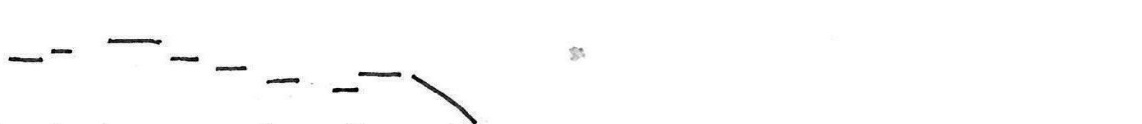
\includegraphics[width=\textwidth]{figures_mod/image12.jpeg}
\gll%
 [%
\linieb{18}{m{\textupsilon}a}
\textstyleEmphasizedVernacularWords{%
\linieb{22}{ˈnaː}%
\linieb{20}{re}%
\linieb{18}{we}%
\linieb{16}{=ke}
} 
\linieb{12}{e}\linieb{14}{ˈka}%
\dline{14}{2}{16}p-o-k%
] \\
man  who=\textsc{cf}  come-\textsc{pa}-3s      \\
\glt`Who came?'
\z
}

\newpage	
The only instance where there can be any rising intonation sentence-finally is a polar question.  It is only used when the speaker is uncertain whether the answer is going to be affirmative or negative \REF{ex:2:x902}.  The rise is on the question clitic =\textstyleStyleVernacularWordsItalic{i}.  



\xbox{\textwidth}{
\ea%x902
\label{ex:2:x902}
% 
\includegraphics[width=\textwidth]{figures_mod/image13.jpeg}
\gll %
[%
\linieb{20}{ˈau}%
\linieb{18}{wa}
\textstyleEmphasizedVernacularWords{%
\linieb{14}{e}%
\linieb{16}{ˈka}%
\dline{16}{2}{24}%
p-o-k=%
\rise{8}%
i%
}%
]\\
 father  come-\textsc{pa}-3s=\textsc{qm}     \\
\glt`Did father come?'
\z
}

If the speaker strongly expects the answer to agree with the polarity of the question, the intonation is falling \REF{ex:2:x903}. Since polar questions are are also marked with a question marker \textstyleStyleVernacularWordsItalic{=}\textstyleStyleVernacularWordsItalic{i} sentence-finally, a separate intonation pattern is partly redundant.



\xbox{\textwidth}{
\ea%x903
\label{ex:2:x903}
% 
\includegraphics[width=\textwidth]{figures_mod/image14.jpeg}
\gll%
 [%
\linieb{20}{ˈau}%
\linieb{18}{wa}
\textstyleEmphasizedVernacularWords{%
\linieb{14}{e}%
\linieb{16}{ˈka}%
\dline{16}{2}{26}{p-o-k=i}}%
] \\
 father  come-\textsc{pa}-3s=\textsc{qm}     \\ 
\glt`Did father come?' (Expecting ``yes'' as an answer.)
\z
}

The intonation pattern in medial clauses, instead of falling at the end, is either level or slightly rising.  The more expected the sequence, the more level the intonation is. In \REF{ex:2:x904} the two clauses are part of an ``expectancy chain'', because coconuts are scraped only for preparing food. (In the following three examples, the medial and subordinate clauses are bolded rather than the verb of the finite clause.)


 

\xbox{\textwidth}{
\ea%x904
\label{ex:2:x904}
% 
\includegraphics[width=\textwidth]{figures_mod/image15.jpeg}
\gll [\textstyleEmphasizedVernacularWords{%
\linieb{18}{iˈ}%
\linieb{20}{we}%
\linieb{16}{ra}
} %
\textstyleEmphasizedVernacularWords{%
\linieb{14}{mu}%
-\linieb{14}{ˈep}
}  %
\linieb{10}{maa} %
\linieb{12}{ˈuu}%
\dline{12}{3}{24}p-i-nen] \\
coconut  scrape-\textsc{ss.seq} food  cook-\textsc{Np-fu}.1s      \\
\glt`I will scrape a coconut and cook food.'
\z
}

But \REF{ex:2:x905} tells about an unexpected event, a person finding a turtle when he had just gone fishing; instead of catching it he might have either chosen to leave it or failed to catch it.

 

\xbox{\textwidth}{
\ea%x905
\label{ex:2:x905}
% 
\includegraphics[width=\textwidth]{figures_mod/image16.jpeg}
\gll %
[\textstyleEmphasizedVernacularWords{%
\linieb{24}{pon}
} %
\textstyleEmphasizedVernacularWords{
\linieb{20}{u}%
\linieb{22}{ˈru}%
\dline{22}{2}{10}%
{\textphi-}%
\rise{18}ap
} %
\textstyleEmphasizedVernacularWords{\linieb{16}{ˈaː}%
\dline{16}{2}{12}w-%
\rise{12}ep
} %
\linieb{10}{p-e}%
\linieb{12}{ˈka}%
\dline{12}{2}{18}p-e-m] \\
 turtle  see-\textsc{ss.seq}  take-\textsc{ss.seq} \textsc{bpx}-come-\textsc{pa}-1s     \\
\glt`I saw a turtle, caught it and brought it (here).'
\z
}

\largerpage
The rising intonation is more common in subordinate clauses; in conditional clauses \REF{ex:2:x906} it is particularly noticeable.  As a rule, the more important the speaker considers the clause as a presupposition for the main clause, the more clearly there is an intonational rise clause-finally.  



\xbox{\textwidth}{
\ea%x906
\label{ex:2:x906}
% 
\includegraphics[width=\textwidth]{figures_mod/image17.jpeg}
\gll %
[\textstyleEmphasizedVernacularWords{
\linieb{24}{i}%
\linieb{26}{ˈ{\textphi}a}
}
\textstyleEmphasizedVernacularWords{
\linieb{22}{u}%
\linieb{24}{ˈru}%
\linieb{20}{{\textphi}-i}%
\dline{20}{3}{26}-nen=%
\rise{13}{na}} 
\linieb{14}{ke}%
\linieb{16}{ˈker} %
\linieb{10}{o}%
\linieb{12}{ˈp-i}%
\dline{12}{2}{14}-nen]\\
 snake  see-\textsc{Np-fu}.1s=\textsc{tp}  fear  hold-\textsc{nps}-\textsc{fu}.1s\\
\glt`If I see a snake, I will be afraid.'
\z
}

A phrase that is fronted as a left-dislocated theme (\sectref{sec:9.1}) also has a rising intonation at the end of the phrase.  The phrase, bolded in \REF{ex:2:x907}, occurs at the beginning of the clause.  The slash indicates a pause.

 

\xbox{\textwidth}{
\ea%x907
\label{ex:2:x907}
% 
\includegraphics[width=\textwidth]{figures_mod/image18.jpeg}
\gll %
[\textstyleEmphasizedVernacularWords{%
\linieb{28}{ˈjos}%
\linieb{24}{=n}%
\rise{26}a
%
}/
\linieb{20}{ o}%
\linieb{24}{ˈwow} %
\linieb{18}{ma}%
\linieb{20}{ˈne}%
\linieb{16}{ka}
\linieb{14}{me}
\linieb{10}{i}%
\linieb{12}{ˈki}%
\linieb{10}{w-i}%
\dline{10}{3}{16}-jem] \\
1s.\textsc{fc}=\textsc{tp}  village  big  not  go-\textsc{Np-}\textsc{pr}.1s      \\
\glt`As for me, I don't go to town.'
\z
}
  
In listing, the intonation rises very slightly at the final syllable of each non-final phrase listed, or is retained at the same level as the previous syllable(s) \REF{ex:2:x908}.


 
\xbox{\textwidth}{
\ea%x908
\label{ex:2:x908}
% 
\includegraphics[width=\textwidth]{figures_mod/image19.jpeg}
\gll%
[\linieb{40}{maː}
\linieb{34}{u}%
\linieb{38}{ˈno}%
\linieb{36}{wa}
\linieb{32}{se}%
\linieb{34}{ˈse}%
\linieb{30}{na}%
\dline{30}{3}{20}{r-e-m}/ %
 \textstyleEmphasizedVernacularWords{
 \linieb{26}{o}%
 \dline{26}{2}{18}{ˈwor}%
 \rise{18}{a}}/ %
 \textstyleEmphasizedVernacularWords{
 \linieb{22}{a}%
 \dline{22}{2}{16}{ˈ{\textphi}ur}%
 \rise{15}{a}}/ %
\textstyleEmphasizedVernacularWords{
\linieb{18}{e}%
\dline{18}{2}{14}{ˈpis}%
\linieb{10}{ow}%
\rise{12}{a}%
}/ %
 \linieb{12}{a}%
\linieb{14}{ˈria} 
\linieb{12}{mo}%
\dline{12}{2}{12}ˈma] \\
thing  many  buy-\textsc{pa}-1s  betelnut  lime  tobacco  alright  taro      \\
\glt`I bought many things: betelnut, lime, tobacco and taro.'
\z
}

A polite way of calling a person, of getting someone's attention, is to call the name or relationship term in such a way that the stressed syllable has a slight rise and a sharp fall in pitch, and following unstressed syllables, if any, have a low pitch \REF{ex:2:x909}.



\xbox{\textwidth}{
\ea%x909
\label{ex:2:x909}
% 
\includegraphics[width=\textwidth]{figures_mod/image20.jpeg}\\
\gll%
[\linieb{22}{eˈ}%
\dline{22}{1}{10}{re}%
\linieb{10}{me}%
\linieb{8}{na}] \\
nephew      \\
\glt`Nephew!'
\z
}

An impatient or exasperated call, or a call for someone distant, has a different pattern.  The voice is louder, the pitch is retained relatively high and level, and the last syllable gets lengthened and, if unstressed, receives a stress almost as strong as that of the stressed syllable \REF{ex:2:x910}.

 

\xbox{\textwidth}{
\ea%x910
\label{ex:2:x910}
% 
\includegraphics[width=\textwidth]{figures_mod/image21.jpeg}
\gll%
 [\linieb{22}{ˈai}%
\linieb{18}{teeee}] \\
mother      \\
\glt`Mother!'
\z
}

Anger is typically expressed by shouting.  The intonation stays fairly level, and the sentence is short and produced in a staccato manner.

Disgust or impatience is expressed by sentence-final interjection \textstyleStyleVernacularWordsItalic{yaa} [jaː], which retains a fairly level pitch and can be lengthened considerably \REF{ex:2:x911}.  An impatient reaction to someone else's words or actions is expressed by sentence-initial interjection \textstyleStyleVernacularWordsItalic{se}, which has a very sharp falling intonation \REF{ex:2:x912}.



\xbox{\textwidth}{
\ea%x911
\label{ex:2:x911}
% 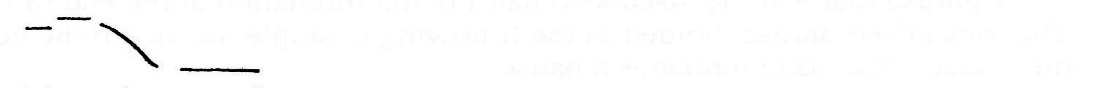
\includegraphics[width=\textwidth]{figures_mod/image22.jpeg}
\gll %
[\linieb{18}{iˈ}%
\linieb{20}{ki}%
\dline{20}{2}{24}{w-eka} %
\linieb{8}{jaaaa}] \\
go-\textsc{imp}.2p \textsc{intj}\\
\glt`Go, for heaven's sake!'
\z
}


 
\xbox{\textwidth}{
\ea%x912
\label{ex:2:x912}
% 
\includegraphics[width=\textwidth]{figures_mod/image23.jpeg}
\gll%
 [\dline{20}{2}{15}{se} 
 \linieb{14}{naːp} 
 \textstyleEmphasizedVernacularWords{
 \linieb{12}{ˈme}
 } %
 \dline{12}{3}{18}ma-e] \\
\textsc{intj} thus  not  say-\textsc{imp}.2s      \\
\glt`Goodness, don't say like that.'
\z
}

\subsection{Orthographic symbols}
%%\hypertarget{RefHeading18821935131865}


\tabref{tab:4:orthosymbols} shows the orthographic symbols for the phonemes. The semivowel /j/ is written as \textstyleStyleVernacularWordsItalic{y} due to the influence of Tok Pisin and English.  Because the orthography represents the phoneme inventory so closely, it is the orthographic symbols that are used in the vernacular examples throughout this thesis after the phonology chapter.


\begin{table}
\caption{Orthographic symbols for Mauwake phonemes}
\label{tab:4:orthosymbols}
\resizebox{\textwidth}{!}{\begin{tabular}{lcccccccccccccc}
\lsptoprule
Consonant phonemes & p & t & k & b & d & g & m & n & {\textphi} & s & l & r & w & j\\
Orthographic representation & p & t & k & b & d & g & m & n & f & s & l & r & w & y\\
\midrule
Vowel phonemes & i & e & a & o & u & \multicolumn{9}{l}{}\\
Orthographic representation & i & e & a & o & u & \multicolumn{9}{l}{}\\
\lspbottomrule
\end{tabular}}
\end{table}

\section{Syllables and phonotactics}\label{sec:2:2}
%%\hypertarget{RefHeading18841935131865}


\subsection{Syllable patterns}
%%\hypertarget{RefHeading18861935131865}


The syllable in Mauwake consists of one or two vowels forming the nucleus, with optional onset and/or coda of one consonant, \textsc{cv} being by far the most frequent syllable structure.\footnote{\citet[13]{Reesink1987} gives a short but good overview of syllable-final consonants in a number of \textsc{tng} languages.} The syllable patterns are given in \tabref{tab:2:syllablepatterns}.

\begin{table}
 \caption{Syllable patterns}
\label{tab:2:syllablepatterns}
\begin{tabular}{ll}
\mytoprule
\textsc{v}  &  \textsc{vc}\\
\textsc{cv} &  \textsc{cvc}\\
\textsc{vv} &  \textsc{vvc}\\
\textsc{cvv} & \textsc{cvvc} \\
\mybottomrule
\end{tabular}
\end{table}

Any vowel can fill the simple nucleus slot of the syllable. The complex nucleus slot is filled either by a geminate vowel or a diphthong. Diphthongs can occur in non-initial syllables too, but geminate vowels cannot. 

Any consonant can fill the onset slot, and all consonants except the voiced plosives, /{\textphi/} and /j/ can fill the coda slot of a syllable. The distribution of the voiced plosives and /{\textphi}/ is also restricted in that they very seldom occur later than in the second syllable of a word and, except for /j/, do not appear in inflectional morphology. \tabref{tab:5:consonantdistr} shows the possible distribution of consonants in a syllable.

\begin{table}
\caption{Consonant distribution in a syllable}
\label{tab:5:consonantdistr}
\setlength{\tabcolsep}{3pt}
\begin{tabular} {crclcccrcl}
\mytoprule
 &\textsc{c} & \textsc{v(v)} & \textsc{c} &&& & \textsc{c} & \textsc{v(v)} & \textsc{c}  \\
\midrule
p & + &    & + &&& n & + && +\\
t & + && + &&& {\textphi} & + && --\\
k & + && + &&& s & + && +\\
b & + && -- &&& l & + && +\\
d & + && -- &&& r & + && +\\
g & + && -- &&& w & + && +\\
m & + && + &&& j & + && --\\
\mybottomrule
\end{tabular}
\end{table} 


\subsection{Vowel sequences}
%\hypertarget{RefHeading18881935131865}

\tabref{tab:6:vowelseq} shows the possible two-vowel sequences in Mauwake. The only possible sequences beginning with either of the two mid vowels are geminate vowels; no other vowel sequences begin with a mid vowel. The other three vowels may combine with any vowel.


\begin{table}
\caption{Vowel sequences}
\label{tab:6:vowelseq}
\begin{tabular}{lllll}
\mytoprule 
ii &  & ai &  & ui\\
ie & ee & ae &  & ue\\
ia &  & aa &  & ua\\
io &  & ao & oo & uo\\
iu &  & au &  & uu\\
\mybottomrule
\end{tabular}
\end{table}

When the second vowel in a vowel sequence is articulatorily the same height or higher than the preceding vowel, the two form a diphthong, i.e., they are part of the same syllable \REF{ex:2:twovowel1}.

\ea
\label{ex:2:twovowel1}
\ea
/kae/  [\textipa{ˈkae}]  `my/our grandfather'
\ex
/kuina/  [\textipa{ˈkui.na}]  `woodborer'
\ex
/aowa/  [\textipa{ˈao.wa}]  `to tie around waist'
\z
\z


When the second vowel is lower than the first, the two vowels form the nuclei of two separate syllables \REF{ex:2:twovowel2}. 

\ea
\label{ex:2:twovowel2}
\ea
/sier/  [\textipa{s{\textsci}.ˈer}]  `husking stick'
\ex
/luaka/  [\textipa{l{\textupsilon}.ˈa.ka}]  `whitebait'
\ex
/kia/  [\textipa{k{\textsci}.ˈa}]  `white'
\z
\z


The high back vowel /u/ is considered lower than the high front vowel /i/, as it behaves similarly to the non-high vowels when following /i/ \REF{ex:2:twovowel3}.

\ea
\label{ex:2:twovowel3}
/niuk/  [\textipa{n{\textsci}.ˈuk}]  `let them give you'
\z

In an open syllable, all the diphthongs allowed by the language are possible. In a closed syllable, /ao/ is the only diphthong that has not been found; but it is very infrequent in an open syllable too. 

Sequences with three vowels are rare: /uau/ and /uai/ are the only ones I have found, and these only occur at morpheme breaks (marked with a hyphen in the examples), and there is a syllable break within the sequence as well \REF{ex:2:threevowels}.\footnote{A syllable break does not need to coincide with a morpheme break; in the examples above it does not.}  

\ea \label{ex:2:threevowels}
\ea
/kua-i-jem/    [\textipa{k{\textupsilon}.ˈai.jem}]      `I build'
\ex
/kua-uk/      [\textipa{k{\textupsilon}.ˈauk}]      `let them build'
\z
\z

\subsection{Consonant sequences} \label{sec:2.2.3}
%\hypertarget{RefHeading18901935131865}

No consonant sequences occur word-initially or -finally. In words with three or more syllables there are some word-medial clusters, which I believe to have resulted from vowel elision.  A vowel may be elided from a non-final syllable immediately following a stressed syllable, which is probably the least prominent syllable in the whole word.\footnote{According to \citet[11]{Sommerstein1977} this is a common process in languages.} It is mainly the high vowels that are dropped, since they are the least sonorant \REF{ex:2:vowelelision}. 

\ea
\label{ex:2:vowelelision}
\ea
/ikemika/  [\textipa{iˈkemka}]  `wound (nn)' 
\ex
/aakisa/  [\textipa{ˈaːksa}]  `now, today'
\ex
/pisikulaw/  [\textipa{piˈsiklaw}]  `grasshopper sp.'
\z
\z


A non-high vowel can also be elided if the adjacent stressed syllable has an identical vowel \REF{ex:2:vowelelisiontwo}:

\ea
\label{ex:2:vowelelisiontwo}
\ea
/kerekenam/  [\textipa{keˈreknam}]  `dollar bird'
\ex
/toonowaw/  [\textipa{ˈtoːnwaw}]  `honey eater'
\z
\z


Occasionally vowel elision takes place in a later syllable than that immediately following the stressed syllable \REF{ex:2:vowelelisionthree}: 

\ea
\label{ex:2:vowelelisionthree}
\ea
/o{\textphi}a{\textphi}ilika/  [\textipa{oˈ{\textphi}a{\textphi}ilka}]  `butterfly'
\ex
/aakuniwikin/  [\textipa{aːkuniwkin}]  `talk.2/3p.\textsc{ds}'
\z
\z

In some of these words the original vowel can still be perceived in slow pronunciation, but in others it has disappeared. Consequently, phonemic vowel clusters are currently developing in Mauwake,\footnote{The present orthography reflects this development in that consonant clusters are written especially 1) where the quality of the elided vowel cannot be established, and/or 2) when the elided form is in very frequent use.} and the distribution of \textsc{cvc} syllables is being extended to include word-medial position as well, and that of \textsc{vvc} and \textsc{cvvc} to include initial position in two-syllable words that have earlier had three syllables (\sectref{sec:2.3.2}).

No clear rules have been found for the site of the vowel elision, but some tendencies are as follows. Nouns have more elision than verb stems. A vowel is dropped much more often between non-homorganic than homorganic consonants. The voiceless velar plosive /k/ is the most frequent phoneme on either side of the elided vowel.

\section{Word}\label{sec:2.3}
%\hypertarget{RefHeading18921935131865}

\subsection{Defining a phonological word in Mauwake}
%\hypertarget{RefHeading18941935131865}

A phonological word is defined on the basis of a primary stress. Words are composed of one or more syllables. The number of syllables seldom exceeds ten, but compound words can be longer. A majority of the words have two or three syllables.  Every word has one syllable with a primary stress, and usually one or more unstressed syllables. 

In words of two or more syllables, the syllable containing the second vowel is stressed. Thus the first syllable is stressed if it contains a geminate vowel (\ref{ex:2:stressone}a) or a diphthong (\ref{ex:2:stressone}b). In all the other cases the second syllable is stressed (\ref{ex:2:stressone}c). When the stressed syllable is long, the stress falls equally on the whole vowel sequence (\ref{ex:2:stressone}d--e). 

\ea
\label{ex:2:stressone}
\ea
/aasa/  [\textipa{ˈaː.sa}]  `canoe'
\ex
/kuija/  [\textipa{ˈkui.ja}]  `it bites'
\ex
/a{\textphi}ura/  [\textipa{a.{ˈ}{\textphi}u.ra}]  `lime'
\ex
/siowa/  [\textipa{si.ˈo.wa}]  `dog'
\ex
/isaimija/  [\textipa{i.ˈsai.mi.ja}]  `(s)he heats (food)'
\z
\z

Both derivational and inflectional affixes may receive primary stress provided they are in a position where stress is normally placed \REF{ex:2:stresstwo}:

\ea
\label{ex:2:stresstwo}
\ea
  /aw-om-e/\\
  {}[\textipa{a.ˈwo.me}]  \\
weave-\textsc{ben}-\textsc{bnfy1}.\textsc{imp}.2s\\
\glt `weave it for me' 

\ex
  /um-o-k/ \\
 {}[\textipa{u.ˈmok}]  \\
die-\textsc{pa}-3s \\
\glt `(s)he died'
\z
\z



Clitics, on the other hand, never receive stress placement. Grammatically they are words, but phonologically they attach to the preceding word. If the preceding word is monosyllabic and has a short vowel, it still takes the primary stress when a clitic is added. The unmarked pronouns are a case in point: they retain their stress when clitics are added. Some non-phonemic lengthening takes place in the vowel of the pronoun stem \REF{ex:2:stressthree}.

\ea
\label{ex:2:stressthree}
\ea
/jo=ko/  [\textipa{ˈjo{\.{}.ko}}]  `\textit{I} (with neutral focus)'
\ex
/jos=ke/  [\textipa{ˈjo{\.{}s.ke}}]  `\textit{I} (and not someone else)' 
\z
\z

Compound words and some reduplicated words also have a secondary stress.  In the second (and third) compound of a compound word, that syllable has a secondary stress which in a single word would receive primary stress \REF{ex:2:stressfour}. 

\ea
\label{ex:2:stressfour}
\ea
/soomare-jiawem-ikemik/  [\textipa{ˈsoːmare-j{\textsci}{ˈ}{ˈ}awem-i{ˈ}{ˈ}kemik}]  `we were walking around'
\ex
/suuw-orom-ikua/  [\textipa{ˈsuːw-o{ˈ}{ˈ}rom-i{ˈ}{ˈ}kua}]  `he is pushing it down'
\z
\z

In those words where a long initial syllable is reduplicated as a whole, the second syllable is also long and receives a secondary stress \REF{ex:2:stressfive}:

\ea
\label{ex:2:stressfive}
\ea
/kui-kuisow/  [\textipa{ˈkui.{ˈ}{ˈ}kui.sow}]  `a few'
\ex
/suu-suusia/  [\textipa{ˈsuː.{ˈ}{ˈ}suː.sia}]  `thorny'
\z
\z

\subsection{Distribution of syllables in a word}\label{sec:2.3.2}
%\hypertarget{RefHeading18961935131865}

All syllable types except  \textsc{vc} can form a monosyllabic word. In polysyllabic words, the occurrence of a certain syllable type is determined by both its position in the word and the stress. 

\tabref{tab:7:syllabletypes} shows what syllable types occur in which positions in a word.  A blank space indicates that the syllable type does not occur in that particular word position at all, and parentheses indicate a rare occurrence. Double parentheses indicate new positions for closed syllables formed as a result of vowel elision (see \sectref{sec:2.2.3}). ``2nd'' indicates the second non-final syllable, and ``3rd-'' stands for the third or later non-final syllable in a polysyllabic word.


\begin{table}
\caption{Distribution of syllable types}
\label{tab:7:syllabletypes}
  \begin{tabular}{lcccccccccc}
  \mytoprule
  \multirow{2}{*}{\parbox{1cm}{Syllable\\type}} & \multicolumn{3}{c}{Stressed syllables} &  & \multicolumn{4}{c}{Unstressed syllables}  &  & \multirow{2}{*}{\parbox{1.2cm}{\mbox{The only} \mbox{syllable}}}\\
  & Initial & 2nd & Final &  & Initial & 2nd & 3rd- & Final &  & \\
  \midrule
  \textsc{v} &  & + & + &  & + &  & + & + &  & +\\
  \textsc{cv} &  & + & + &  & + & + & + & + &  & +\\
  \textsc{vv} & + & (+) & (+) &  &  &  & (+) & + &  & +\\
  \textsc{cvv} & + & + & (+) &  &  &  & + &  &  & +\\
  \textsc{vc} &  &  & + &  &  &  &  & + &  & \\
  \textsc{cvc} &  & ((+)) & + &  &  & ((+)) & ((+)) & + &  & +\\
  \textsc{vvc} & ((+)) &  & + &  &  &  &  & + &  & +\\
  \textsc{cvvc} & ((+)) &  & + &  &  &  &  & + &  & +\\
  \mybottomrule
  \end{tabular}
\end{table}

\footnotetext{`2nd' indicates the second non-final syllable, and `3rd-' stands for the third or later non-final syllable in a polysyllabic word.}


Some distributional characteristics can be summarised as follows.  The most frequent syllable type, \textsc{cv}, also has the widest distribution: a stressed initial syllable is the only position where it cannot occur, as an initial syllable with a single short vowel is always unstressed. The same reason accounts for the absence of \textsc{v} syllables in the same position. \textsc{v} syllables also never occur after a geminate vowel or diphthong, so they cannot occupy the second unstressed syllable position. A \textsc{vv} syllable in medial or final position is possible but very rare. The two previous statements may be combined to make the claim that there is some resistance towards \textsc{vvv} sequences in Mauwake. The syllables with a consonant coda only occur word finally, except where vowel elision has changed the syllable structure.  

\subsection{Morphophonology}\label{sec:2.3.3}
%\hypertarget{RefHeading18981935131865}

There are not many morphophonological alternations in Mauwake.  The most important is the rule system governing the vowel of the past tense suffix and the medial verb same-subject sequential action and simultaneous action suffixes (called the medial verb suffixes\footnote{There are also other medial verb suffixes, which are not  affected by these morphophonological rules.} in the discussion below).  Others include the change in the verbaliser suffix and the form of the completive aspect marker.

\subsubsection{Elision of word-final vowel}
%\hypertarget{RefHeading19001935131865}

The phoneme /a/ has a very high frequency as the word-final phoneme, particularly in the nouns and adjectives.  It accounts for approximately 85\% of all the vowel-final words.  In normal and fast speech this /a/ is often dropped from an unstressed word-final \textsc{cv} syllable, especially when followed by a word with an initial vowel. The elision rule is in  \REF{ex:2:elisionrule} and examples in \REF{ex:2:elisionexample}. 

\ea
\label{ex:2:elisionrule}
\begin{tabular}{c}\textsc{v}\\+central\\--stress\\    \end{tabular}
\begin{tabular}{c}    $\rightarrow $ {\O}  /  \textsc{c} \_\_  \#  \textsc{v} \\~\\~\\    \end{tabular}
\z

\ea
\label{ex:2:elisionexample}
\ea
/koora unowa/  [\textipa{ˈkoːr  u{ˈ}nowa}]  `many houses'
\ex
/takira {\textphi}aara/  [\textipa{taˈkir  {ˈ}{\textphi}aːra}]  `boys' house'
\ex
/siiwa eliwa/  [\textipa{ˈsiːw  e{ˈ}liva}]  `good/bright moon'
\ex
/ikoka uura/  [\textipa{iˈkok  {ˈ}uːra}]  `later at night'
\z
\z

In some cases even a stressed /a/ is elided, and the stress moves to the following vowel in the utterance.  This mainly happens with the accusative pronouns, which tend towards cliticization \REF{ex:2:stressedelision} (\sectref{sec:3.5.3}).

\ea
\label{ex:2:stressedelision}
/me ne{\textphi}a uru{\textphi}am/  [\textipa{ˈme ne{\textphi} {ˈuru}{\textphi}am}]  `I didn't see you'
\z

In compound words the final /a/ is dropped from the first constituent even when the second begins with a consonant, except when the final syllable of the first constituent is stressed \REF{ex:2:compoundelision}.  

\ea
\label{ex:2:compoundelision}
\ea
/aara muuka/  [\textipa{ˈaːr {ˈ}muːka}]  `chick'
\ex
/emera tapaka/  [\textipa{eˈmer ta{ˈ}paka}]  `sago cake'
\ex
/mera soo/  [\textipa{meˈra {ˈ}soː}]  `fish trap'
\z
\z

\subsubsection{Reduplication}\label{sec:2.3.3.2}
%\hypertarget{RefHeading19021935131865}

There are various patterns of reduplication in Mauwake. With a few exceptions, reduplication takes place at the beginning of the word.  The meaning involves plurality in one way or another; with verbs it indicates repeated action and/or the object of the action ending up in several pieces. Occasionally with adjectives it also indicates enhanced quality (\sectref{sec:3.3}).

How a word is reduplicated can to some extent be predicted from the phonological shape of the word.  Type 1 below is the most common, 2 and 3 are the only possible ones for the words with a short and a long initial vowel respectively.  Reduplication process does not always respect syllable boundaries.

\paragraph[Type 1]{Type 1}
%\hypertarget{RefHeading19041935131865}

Everything up to and including the first vowel of the stressed syllable is reduplicated.  Even with the reduplication these words retain the normal stress pattern: the second syllable of the reduplicated form is stressed, because regardless of whether one or two syllables are reduplicated the first syllable in this type is always short. When two of syllables are reduplicated, the originally stressed syllable of the word root gets a secondary stress \REF{ex:2:reduptypeone}.

\ea
\label{ex:2:reduptypeone}
\ea
/pu-puukija/  [\textipa{pu.ˈpuː.ki.ja}]  `cut into pieces'
\ex
/pu-puija/  [\textipa{pu.ˈpui.ja}]  `break into pieces'
\ex
/pere-perekija/  [\textipa{pe.ˈre.pe.{ˈ}{ˈ}re.ki.ja}]  `tear into pieces'
\ex
/kiri-kiripija/  [\textipa{ki.ˈri.ki.{ˈ}{ˈ}ri.pi.ja}]  `turn round \& round, mix'
\ex
/mane-maneka/  [\textipa{ma.ˈne.ma.{ˈ}{ˈ}ne.ka}]  `(many) big (things)'
\z
\z


\paragraph{Type 2:  \textsc{v}\textsubscript{1}\textsc{c}\textsubscript{1}\textsc{v}\textsubscript{1} - \textsc{v}\textsubscript{1}\textsc{c}\textsubscript{1}\textsc{v}\textsubscript{2}\textsc{c}\textsubscript{2}\textsc{v}(\textsc{v}\textsubscript{3})\textsc{x}}
%\hypertarget{RefHeading19061935131865}

In the words of the second type, the reduplication repeats the initial vowel and consonant of the word root, adding another vowel of the same quality after the consonant.  In these words the stress shifts from the second syllable of the root to the final vowel of the reduplicated element.  Phonetically this vowel usually merges into one with the following vowel, which always has the same quality \REF{ex:2:reduptypetwo}.  Stresswise this creates an interesting pattern, where a syllable with a primary stress is followed by one with secondary stress.  Types 3 and 4 also have this kind of stress pattern.

\ea
\label{ex:2:reduptypetwo}
\ea
/ele-eliwa/  [\textipa{e.ˈle.{ˈ}{ˈ}li.wa}]  `(many) good (things)'
\ex
/ara-arow/  [\textipa{a.ˈra.{ˈ}{ˈ}row}]  `in threes'
\ex
/oko-okaiwi/  [\textipa{o.ˈko.{ˈ}{ˈ}kai.wi}]  `this side and that'
\z
\z

\paragraph{Type 3:  \textsc{v}\textsubscript{1}\textsc{v}\textsubscript{1}\textsc{c}\textsubscript{1} - \textsc{v}\textsubscript{1}\textsc{v}\textsubscript{1}\textsc{c}\textsubscript{1}\textsc{v}\textsubscript{2}\textsc{x}}
%\hypertarget{RefHeading19081935131865}

A very small group of words has this type of reduplication, where the initial geminate vowel and the following consonant are reduplicated.  The result is a word where both the first and the second syllable have a complex nucleus, a word type not allowed in the simple non-reduplicated words.  In these reduplicated words the first syllable receives primary stress and the second syllable secondary stress.  The first syllable has a syllable pattern (\textsc{vvc}) which is not possible for the first syllable in a non-reduplicated polysyllabic word \REF{ex:2:reduptypethree}.

\ea
\label{ex:2:reduptypethree}
\ea
/iiw-iiwa/  [\textipa{ˈiːv.{ˈ}{ˈ} iː.va}]  `(many) short (things)'
\ex
/iin-iinan/  [\textipa{ˈiːn.{ˈ}{ˈ} iː.nan}]  `(the things) high up'
\z
\z

\paragraph{Type 4:  \textsc{c}\textsubscript{1}\textsc{v}\textsubscript{1}\textsc{v}\textsubscript{2} - \textsc{c}\textsubscript{1}\textsc{v}\textsubscript{1}\textsc{v}\textsubscript{2}\textsc{x}}
%\hypertarget{RefHeading19101935131865}

In this type the long first syllable is repeated entirely, but nothing else.  The two vowels in the initial syllable may be identical or different in quality \REF{ex:2:reduptypefour}. This is not a very common pattern.

\ea
\label{ex:2:reduptypefour}
\ea
/kui-kuisow/  [\textipa{ˈkui.{ˈ}{ˈ}kui.sow}]  `a few'
\ex
/soo-soomarija/  [\textipa{ˈsoː.{ˈ}{ˈ}soː.ma.ri.ja}]  `amble, stroll'
\z
\z

\paragraph{Unusual reduplications}
%\hypertarget{RefHeading19121935131865}

The word \textstyleStyleVernacularWordsItalic{gelemuta} `small' has two unusual reduplicated forms, where the end of the word is changed: \textstyleStyleVernacularWordsItalic{gelemutitik} and \textstyleStyleVernacularWordsItalic{gelemutumut} `(many) small (things)'.  Type 1 reduplication rule can also be applied to these already reduplicated forms, although not to the root \REF{ex:2:redupgelemuta}.

\ea
\label{ex:2:redupgelemuta}
\ea
/gele-gelemutitik/  [\textipa{ge.ˈle.ge.{ˈ}{ˈ}le.mu.ti.tik}]  `very small (pl.)'
\ex
*/gele-gelemuta/
\z
\z

The verb \textstyleStyleVernacularWordsItalic{wafuriya} `throw' also has an irregular reduplicated form: only the second syllable is reduplicated \REF{ex:2:redupwafuriya}.

\ea
\label{ex:2:redupwafuriya}
/wa{\textphi}u{\textphi}urija/  [\textipa{va.ˈ{\textphi}u.{\textphi}u.ri.ja}]  `throw around'
\z

The reduplication for the word \textstyleStyleVernacularWordsItalic{owowa} `village' occurs at the beginning of the word, but it does not follow any of the patterns above \REF{ex:2:redupowowa}. So far it is the only one of its kind found.

\ea
\label{ex:2:redupowowa}
/owow-owowa/  [\textipa{o.ˈwo.wo{ˈ}{ˈ}wo.wa}]  `(many/all) villages'
\z

Mauwake has a number of nouns of the following the pattern \textsc{c}\textsubscript{1}\textsc{v}\textsubscript{1}\textsc{c}\textsubscript{2}\textsc{v}\textsubscript{2} \textsc{c}\textsubscript{1}\textsc{v}\textsubscript{1}\textsc{c}\textsubscript{2} , which looks like reduplication, but with the word-final vowel deleted.  However, these words do not have any semantic relationship with a corresponding \textsc{c}\textsubscript{1}\textsc{v}\textsubscript{1}\textsc{c}\textsubscript{2}\textsc{v}\textsubscript{2} word in cases where the latter may exist.  Words of this type are not considered to have resulted from reduplication \REF{ex:2:nonredup}.

\ea
\label{ex:2:nonredup}
\ea
/mulamul/  [\textipa{muˈlamul}]  `trevally'
\ex
/jawejaw/  [\textipa{jaˈvejav}]  `hunting magic'
\z
\z

Similarly, words of the pattern \textsc{c}\textsubscript{1}\textsc{v}\textsubscript{1}\textsc{c}\textsubscript{1}\textsc{v}\textsubscript{1}\textsc{c}\textsubscript{2}\textsc{v}\textsubscript{2} are not considered reduplicated forms \REF{ex:2:nonredup2}.  Firstly, there is no semantic relationship with a corresponding \textsc{c}\textsubscript{1}\textsc{v}\textsubscript{1}\textsc{c}\textsubscript{2}\textsc{v}\textsubscript{2} word, even if the latter exists. Secondly, in Mauwake there is a very strong tendency to have the same vowel in the first two syllables of trisyllabic or longer words, whether the consonant is the same or not. 

\ea
\label{ex:2:nonredup2}
\ea
/momora/  [\textipa{moˈmo.ra}]  `fool(ish)'
\ex
/sisina/  [\textipa{siˈsi.na}]  `edge'
\z
\z

\subsubsection{Past tense and medial verb suffixes}\label{sec:2.3.3.3}
%\hypertarget{RefHeading19141935131865}


There are three past tense verb suffixes for second and third person singular forms, -\textstyleStyleVernacularWordsItalic{a}, -\textstyleStyleVernacularWordsItalic{e} and -\textstyleStyleVernacularWordsItalic{o}.  Which one is chosen for which verb is determined mainly by the phonemes in the stem final syllable.\footnote{Most of these rules were originally worked out by Kwan Poh San.}

The two basic allomorphs for the past tense suffix are \{-a\} and \{-\textsc{e}\}. /\textstyleStyleVernacularWordsItalic{-}o/ is a subgroup of the allomorph \{-\textsc{e}\}. The subgrouping is based on the fact that the \textstyleStyleVernacularWordsItalic{-a/}\textstyleStyleVernacularWordsItalic{-e} distinction runs through the whole past tense paradigms and occurs in the medial verb suffixes as well, whereas the \textstyleStyleVernacularWordsItalic{-}\textstyleStyleVernacularWordsItalic{e/-o} distinction only occurs in the second and third person past tense forms of some verbs.  According to the rounding rule below \REF{ex:2:pasttenseruleEo}, \{-\textsc{e}\} is realized as /-o/ when both following a [+ labial] phoneme (either a labial consonant or the high rounded vowel /u/) and preceding a non-labial consonant \REF{ex:2:Eoex}. 

\ea
\label{ex:2:pasttenseruleEo}
\{\textsc{e}\} {{\textgreater}} /o/  /  \textsc{x} \textsubscript{\textsc{lab}}  \_\_  \textsc{c}\textsubscript{\textsc{non-lab}} 
\z

\ea
\label{ex:2:Eoex}
\ea
/aaw-o-k/  `(s)he got (it)'  cf.  /aaw-e-m/  `I got (it)'
\ex
/mu-o-n/  `you swallowed'  cf.  /mu-e-m/  `I swallowed'
\z
\z

The discussion below only mentions the past tense suffixes. The vowels in the  the medial verb suffixes are the same but do not have the allophonic variation between /-e/ and /-o/.  

The morphophonological rules governing the choice of past tense suffixes are listed in their order of relative strength, with regard to the number of cases in the data\footnote{The count included 273 verbs with the past tense suffix {\nobreakdash-\textstyleStyleVernacularWordsItalic{a}},  364 with the suffix -\textstyleStyleVernacularWordsItalic{e}.} as well as the number of exceptions.

\ea
\textstyleEmphasizedWords{{Rule 1}}.  With a stem-final high vowel /i/ or /u/, the past tense suffix is always \{\nobreakdash-\textsc{e}\} \REF{ex:2:rule1ex}.
\z


\ea
\label{ex:2:rule1ex}
\ea
/waki-\textstyleEmphasizedVernacularWords{e}-k/  `(s)he fell down'
\ex
/nepi-\textstyleEmphasizedVernacularWords{e}-k/  `(s)he raised animals'
\ex
/mu-\textstyleEmphasizedVernacularWords{o}-k/  `(s)he swallowed'
\ex
/karu-\textstyleEmphasizedVernacularWords{o}-k/  `(s)he ran'
\z
\z

\ea
\textstyleEmphasizedWords{{Rule 2}}.  With a stem-final alveolar nasal /n/, the suffix is nearly always /-e/ \REF{ex:2:rule2ex}.
\z

\ea
\label{ex:2:rule2ex}
\ea
/kekan-\textstyleEmphasizedVernacularWords{e}-k/  `it hardened'
\ex
/peren-\textstyleEmphasizedVernacularWords{e}-k/  `it tore'
\ex
/riirin-\textstyleEmphasizedVernacularWords{e}-k/  `(s)he laughed'
\ex
/solon-\textstyleEmphasizedVernacularWords{e}-k/  `it glided'
\ex
/uuwun-\textstyleEmphasizedVernacularWords{e}-k/  `(s)he chatted'
\z
\z

In the data there are 128 verb stems ending in /n/, and only 15 take the suffix \{\nobreakdash-a\}. In some cases there is a conflict between rules 2 and 3 (below), and 13 of those exceptions follow Rule 3.

\ea
\textstyleEmphasizedWords{{Rule 3.} } When the stem final syllable has a low vowel, there is dissimilation between the vowels in the stem final syllable and the past tense suffix. For these morphophonological rules the mid vowels are also considered low, so that there is height distinction only between high and low vowels.
\z

\ea
\begin{tabular}{c}X \\~ \\~ \end{tabular}
\begin{tabular}{c}V \\ +low\\{\textalpha} central \end{tabular}
\begin{tabular}{c}(C) \\~ \\~ \end{tabular}
\begin{tabular}{c}+ \\~ \\~ \end{tabular}
\begin{tabular}{c}\textbf{V} \\ +low\\-{\textalpha} central \end{tabular}
\z

The past tense suffix tends to be \{-a\}, when the last vowel in the stem is /e/ or /o/ \REF{ex:2:rule3ex}. 

\ea
\label{ex:2:rule3ex}
\ea
/aner-\textstyleEmphasizedVernacularWords{a}-k/  `(s)he aimed at'
\ex
/sirek-\textstyleEmphasizedVernacularWords{a}-k/  `it scratched'
\ex
/imen-\textstyleEmphasizedVernacularWords{a}-k/  `(s)he found
\ex
/on-\textstyleEmphasizedVernacularWords{a}-k/  `(s)he did/made'
\ex
/soop-\textstyleEmphasizedVernacularWords{a}-k/  `(s)he buried'
\z
\z

In words with /a/ as the last vowel in the stem, the past tense suffix tends to be \{\nobreakdash-\textsc{e}\} \REF{ex:2:rule3exx}.\footnote{In the data there are 187 verbs that follow this rule and 19 that do not.}

\ea
\label{ex:2:rule3exx}
\ea
/serak-\textstyleEmphasizedVernacularWords{e}-k/  `(s)he wiped'
\ex
/war-\textstyleEmphasizedVernacularWords{e}-k/  `(s)he killed it'
\ex
/ma-\textstyleEmphasizedVernacularWords{e}-k/  `(s)he said'
\ex
/ekap-\textstyleEmphasizedVernacularWords{o}-k/  `(s)he came'
\ex
/aaw-\textstyleEmphasizedVernacularWords{o}-k/  `(s)he got/took'
\z
\z

\ea
\textstyleEmphasizedWords{{Rule 4}}. When a high vowel is followed by a stem-final consonant /k/, /t/, /s/, /r/ or /l/, the past tense suffix is \{-a\}.  This group of consonants includes nearly all of the non-labial consonant phonemes; /n/ is handled in Rule 2, the voiced stops never occur stem-finally and /j/ hardly ever does \REF{ex:2:rule4ex}.  
\z

\ea
\label{ex:2:rule4ex}
\ea
/puuk-\textstyleEmphasizedVernacularWords{a}-k/  `(s)he cut'
\ex
/mik-\textstyleEmphasizedVernacularWords{a}-k/  `(s)he speared'
\ex
/itit-\textstyleEmphasizedVernacularWords{a}-k/  `(s)he smashed'
\ex
/anetir-\textstyleEmphasizedVernacularWords{a}-k/  `(s)he tied'
\ex
/{\textphi}uur-\textstyleEmphasizedVernacularWords{a}-k/  `(s)he blew'
\ex
/a{\textphi}ilil-\textstyleEmphasizedVernacularWords{a}-k/  `it was sweet'
\z
\z

With the rest of the verbs, i.e. total of about 25\% of all the basic verbs, it is very difficult to find any rules governing the choice of the past tense suffix \REF{ex:2:norule}.

\ea
\label{ex:2:norule}
\ea
/tiim-\textstyleEmphasizedVernacularWords{a}-k/  `(s)he touched'
\ex
/aru{\textphi}-\textstyleEmphasizedVernacularWords{a}-k/  `(s)he hit'
\ex
/oosip-\textstyleEmphasizedVernacularWords{o}-k/   `(s)he sweated'
\ex
/{\textphi}iririm-\textstyleEmphasizedVernacularWords{o}-k/  `(s)he squeezed'
\ex
/u{\textphi}-\textstyleEmphasizedVernacularWords{o}-k/  `(s)he danced'
\ex
/iw-\textstyleEmphasizedVernacularWords{o}-k/  `(s)he gave him/her'
\z
\z

A few verbs apparently have dropped the past tense suffix altogether.  Most of these have the stem ending in the vowel sequence /ua/ \REF{ex:2:nopasttensesuffix}:

\ea
\label{ex:2:nopasttensesuffix}
\ea
/kua-{\O-k}/  `he built'
\ex
/wua-{\O-k}/  `(s)he put'
\ex
/piipua-{\O-k}/  `(s)he left'
\z
\z

Another verb where the past tense suffix vowel seems to have disappeared is /oro-{\O}-k/ `(s)he went down'.  If the second vowel were to be taken as the suffix this verb would defy the basic rules, since the vowel /o/ is retained right through the past tense paradigm, and with the root vowel /o/ the suffix should be \{-a\}.  Positing /oro-/ as the root solves the question why the present tense form is /ora-/: since /oi/ is not a permitted vowel sequence on Mauwake, the low back vowel /o/ has changed into the low central vowel /a/ when preceding the high front vowel /i/ of the present tense suffix.

The verbs in the Mauwake dictionary are marked as belonging to Class 1 or Class 2, the former taking \{-a\} and the latter \{-\textsc{e}\} as the past tense suffix. This is because of the following reasons: 1) the rules are rather complicated, 2) there are a number of exceptions to the main rules, and 3) there are pairs of homophonous verb roots that take a different past tense suffix each \REF{ex:2:homophonousroots}.

\ea
\label{ex:2:homophonousroots}
\ea
/iw-\textstyleEmphasizedVernacularWords{a}-k/  `(s)he went'
\ex
/iw-\textstyleEmphasizedVernacularWords{o}-k/  `(s)he gave him/her'
\ex
/miim-\textstyleEmphasizedVernacularWords{a}-k/  `(s)he heard'
\ex
/miim-\textstyleEmphasizedVernacularWords{o}-k/  `(s)he preceded'
\ex
/op-\textstyleEmphasizedVernacularWords{a}-k/  `(s)he held'
\ex
/op-\textstyleEmphasizedVernacularWords{o}-k/  `it boiled'
\ex
/keen-\textstyleEmphasizedVernacularWords{a}-k/  `it touched'
\ex
/keen-\textstyleEmphasizedVernacularWords{e}-k/  `it was hot'
\z
\z

\subsubsection{Inchoative suffix} \label{sec:2.3.3.4}
%\hypertarget{RefHeading19161935131865}

The verbalizer for both adjectives and nouns is the inchoative suffix \{-a\textsc{r}\}, the root of the verb `to become' (\sectref{sec:3.8.2.2.2}).  In most environments it is realized as /\nobreakdash-ar/, but becomes /-al/ when the last syllable of the root contains the lateral consonant /l/ \REF{ex:2:inchoative}.  An illustrative example is the word \textstyleStyleVernacularWordsItalic{samora/damola} `bad', which takes a different verbalizer depending on the root allomorph.

\ea
\label{ex:2:inchoative}
\ea
/supuk\textstyleEmphasizedVernacularWords{-ar}-e-k/  `it got wet' 
\ex
/duduw-\textstyleEmphasizedVernacularWords{ar}-e-k/  `it became blunt'
\ex
/samor-\textstyleEmphasizedVernacularWords{ar}-e-k/  `it broke/spoiled'
\ex
/damol-\textstyleEmphasizedVernacularWords{al}-e-k/  `it broke/spoiled'
\ex
/memel-\textstyleEmphasizedVernacularWords{al}-e-k/  `it became tame'
\ex
/masi-\textstyleEmphasizedVernacularWords{al}-e-k/  `it became bitter'
\z
\z

In a few cases the inchoative suffix has the form /-al/ although there is no lateral consonant in the root.  This might be expected, since there is some fluctuation between the liquids /l/ and /r/ in Mauwake: /eliwa/ {\Tilde} /eriwa/ `good', /samora/ {\Tilde} /damola/ `bad'.\footnote{In Trans New Guinea, as well as other Papuan, languages it is also very common to have only one liquid, with /l/ and /r/ as allophones of the same phoneme (\citealt[55]{Wurm1982}, \citealt[55]{Foley1986}).} 


\subsubsection{Completive aspect marker}
%\hypertarget{RefHeading19181935131865}

The completive aspect marker (\sectref{sec:3.8.5.1.1.1}) has its origin in the verb for `put', \textstyleStyleVernacularWordsItalic{wua}\nobreakdash-,\footnote{The verb `put' is commonly used as a completive aspect marker in Papuan languages (\sectref{sec:3.8.5.1.1.1}).} but this connection has by now become opaque and the speakers consider it a morpheme on its own, \textstyleStyleVernacularWordsItalic{pu}- \REF{ex:2:completive}.  The initial /p/ results from assimilation with the final /p/ of the same-subject sequential action medial verb form obligatorily preceding the completive morpheme.

\ea
\label{ex:2:completive}
\gll\itshape en-ep  \itshape wu-a-k  {\upshape \textgreater}  \itshape enep-pu-a-k \\ 
eat-\textsc{ss}.\textsc{seq}  put-\textsc{pa}-3s  {{\textgreater}}  eat-\textsc{ss}.\textsc{seq}-\textsc{cmpl}-\textsc{pa}-3s\\
\glt `(s)he ate'
\z

\subsection{Loan words}
%\hypertarget{RefHeading19201935131865}

When words are borrowed from other languages, they are usually made to conform to the Mauwake phonology, if they do not originally do so.  Thus Tok Pisin \textstyleForeignWords{kikim} `kick' becomes \textit{kiikim}- in Mauwake; the word retains the original Tok Pisin word-initial stress, and the vowel in the first syllable becomes a geminate.  The initial glottal fricative /h/ in the original becomes a lengthened vowel in Mauwake, e.g. Tok Pisin \textstyleForeignWords{handet} `hundred' changes into \textstyleStyleVernacularWordsItalic{aandet}  in Mauwake.

The only non-native phoneme regularly retained in the loan word is the velar nasal /{\ng}/, particularly prominent in the neighbouring language, Mala, and also used in personal names \REF{ex:2:Malaloan}:

\ea
\label{ex:2:Malaloan}
/nadi{\ng-ar-e-k/}  `(s)he decorated him/herself'
\z

Since consonant sequences are quite rare in Mauwake, loan words with consonant clusters tend to have vowels inserted between the consonants.  With the ever-growing influence of Tok Pisin, vowel insertion is getting less common.  A combination of a nasal plus a homorganic stop is always retained in a loan word (\tabref{tab:2:loanwords}).

\begin{table} 
 \caption{Loanwords with a combination of nasal plus homorganic stop.}
\label{tab:2:loanwords}
\begin{tabular}{>{\itshape}l>{\itshape}l>{\itshape}l}
\mytoprule
\upshape Tok Pisin   & \upshape Mauwake  & \upshape English\\
\midrule 
glas & galas&  glass \\
{trinde}&  tirinde &  Wednesday \\
{namba} & naamba & number \\
{handet} & aandet & hundred \\
\mybottomrule
\end{tabular}

\end{table}


\renewcommand{\exfont}{\itshape}
\renewcommand{\eachwordone}{\itshape}
%3

\chapter{Morphology}\label{sec:3}
%\hypertarget{RefHeading19221935131865}
{}
\section{Introduction}\label{sec:3:1}
%\hypertarget{RefHeading19241935131865}
{}
A grammatical word in Mauwake is defined on the basis of the following main criteria quoted from \citet[12--14]{Dixon2010b}:

A grammatical word
\begin{itemize}
\item has as its base one or more lexical roots to which morphological processes apply;
\item has a conventionalized coherence and meaning.
\end{itemize}
When a grammatical word involves compounding or affixation, its component grammatical elements 

\begin{itemize}
\item always occur together;
\item generally occur in a fixed order
\end{itemize}

The following supplementary criteria also apply: a word only allows one inflectional affix of any one type (ibid. 15), and in derivation recursiveness is blocked except in the case of causatives (ibid. 16--17). Even here the recursion is more ostensible than real, as it does not add another argument into the clause (\sectref{sec:3.8.2.3.1}). Person/number suffixes act as word-final boundary markers in finite verbs (ibid. 17). Many words, especially those belonging to the major word classes, ``may constitute a complete utterance'' (ibid. 19) by themselves. 

The boundaries of the grammatical and phonological words coincide, except in the case of clitics. Grammatically a clitic is a word but phonologically it is bound to the preceding word.

The classes of nouns, adjectives, personal pronouns, quantifiers, verbs and adverbials can be reasonably clearly defined both morpho-syntactically and semantically. The classes of question words and deictics include words with heterogeneous syntactic behaviour; question words have semantic and functional, and some morphological similarities as a group, whereas the category of deictics is based on strong morphological and semantic similarities. Connectives share the function of conjoining elements on the same level. As ``functor words'' postpositions and especially clitics are dependent on the preceding phrase. Interjections are different from all the other word classes in that they operate outside the normal syntax and often constitute a whole expression by themselves.

Nouns are naturally the largest category, but verbs are morphologically the most complex and interesting word class.

Although the great majority of the words in Mauwake can be assigned to one of the categories above, there is some indeterminacy with regard to some words that seem to belong to two or more word classes and the meanings of which are clearly related.\footnote{In Austronesian languages it is common to have pre-categorial stems that may combine with affixation belonging to various word classes; only the whole word may be assigned to a particular word class.} They are not homonyms, since they are semantically related. Some transitive verbs have been derived by zero derivation from nouns and adjectives, and even from adverbs (§\sectref{sec:3.8.2.2.1}, \ref{sec:3.8.4.4.3}). Nominalized verbs (\sectref{sec:3.2.6.1}) function as nouns or adjectives. At the end of (\sectref{sec:3.2.2}) there is a list of words that are originally nouns but have become adjectives as well. Some non-numeral quantifiers (\sectref{sec:3.4.2}) also function as intensity adverbs (\sectref{sec:3.9.2}). Besides these, there are individual words that function in more than one word class; these are mentioned where they occur.

\section{Nouns}\label{sec:3.2}
%\hypertarget{RefHeading19261935131865}
{}
\subsection{General discussion}\label{sec:3:2:1}
%\hypertarget{RefHeading19281935131865}
{}
Although the traditional semantic definition of the noun as the ``name of a person, place or thing'' is not valid as a basis for assigning members to the class, it still gives a good general description of the prototypical members of the class in Mauwake. In \citegen[63]{Frawley1992} words, ``when the traditional definition is reversed, the definition turns out to be true. Nouns are not always persons, places or things, but persons, places and things always turn out to be nouns.''\footnote{See also \citet[117]{Sapir1921}, \citet[60]{Jespersen1924}, \citet[449]{Lyons1977} and \citet[7]{Schachter1985}.} Recognizing the semantic motivation of the class does not eliminate the need to define the class by its formal or functional properties.

No good morphological definition of nouns is possible in Mauwake, as there is no inflection for number \REF{ex:3:x1}, gender or class,\footnote{Gender or class systems are widespread in Papuan languages \citep[77]{Foley1986}. Especially in the \textsc{tng} languages a covert system is common \citep[58]{Wurm1982}, where the noun class determines what existential verb is used with each noun.} or case, in the noun itself. Especially the lack of plural marking is typical of the nouns in Trans-New Guinea languages \citep[36]{Wurm1982}. The glosses in \REF{ex:3:x1} indicate a singular/plural alternative in the nouns, but the singular form in the glosses of other examples is to be understood as neutral regarding number. 

\ea%x1
\label{ex:3:x1}
\gll siowa wiawi\\
dog(s) father(s)\\
\glt`The dog's/dogs' owner(s)'
\z

Nouns are usually monomorphemic, with the exception of a small group of inalienably possessed nouns (\sectref{sec:3.2.4}), nouns derived from verbs (\sectref{sec:3.2.6.1}), reduplicated nouns (\sectref{sec:3.2.6.2}) and compound nouns (\sectref{sec:3.2.5}). The division into \textstyleEmphasizedWords{count} and \textstyleEmphasizedWords{mass} nouns is not very noticeable. It is mainly shown in the choice between the quantifiers \textstyleStyleVernacularWordsItalic{unowa} `many' and \textstyleStyleVernacularWordsItalic{maneka} `big, much', and to some extent in verb agreement morphology (\sectref{sec:3.4}).

The syntactic function provides the best criterion for defining a noun in Mauwake. Nouns function mainly as the head of a noun phrase, often the head being the only element in the \textstyleAcronymallcaps{np}.\footnote{Sometimes an adjective, a quantifier or a genitive pronoun looks like a head of a \textstyleAcronymallcaps{np}, but those cases are elliptical, and the head noun is recoverable.} They can also function as a qualifier or, more rarely, as a modifier in a \textstyleAcronymallcaps{np}. In \REF{ex:3:x2}, the \textstyleAcronymallcaps{np}s function as subject and object, and are manifested by just nouns.

\ea%x2
\label{ex:3:x2}
\gll Emeria=ke iwera fiirim-i-mik.\\
 woman=\textsc{cf} coconut gather-Np-\textsc{pr}.1/3p\\
\glt`(The) women gather coconuts.'
\z

\citet[710]{HopperEtAl1984} also maintain that {``from the discourse point of view, nouns function to introduce participants and `props' and to deploy them.''}\footnote{Actually this is the function of a \textsc{np} rather than a noun.} This is true in Mauwake as well, but it is not used as a criterion for defining the nouns.

\subsection{Nouns and adjectives: one or two word classes?}\label{sec:3.2.2}
%\hypertarget{RefHeading19301935131865}
{}
Since adjectives in Mauwake are phonologically, morphologically and syntactically very similar to nouns, the question must be asked whether the two form just one class of nominals or whether they belong to two separate word classes. In the following discussion they are treated on a semantic basis as if they were separate classes, i.e. certain words are called nouns and others adjectives, but a final conclusion as to their status is not drawn until the end of the section.

A \textstyleEmphasizedWords{{phonologically}} interesting feature common to nouns and adjectives is that the majority of both end in the vowel <a>.\footnote{In the other word classes words ending in <a> do occur but they are very infrequent.} Inside noun phrases this vowel, when unstressed, is usually elided preceding a vowel and often also preceding a consonant. In cases like \REF{ex:3:x3}, where there are two or more possible places for elision, the vowel most easily drops at the end of an adjective preceding an intensifier. Elision is also acceptable in two or more sites within one \textstyleAcronymallcaps{np}; this is shown in  \REF{ex:3:x3} and \REF{ex:3:x4}. 

\ea%x3
\label{ex:3:x3}
\gll koora eliw(a) akena  {\upshape also:} koor(a) eliw(a) akena \\
house good very\\
\glt`a very good house'
\z

\ea%x4
\label{ex:3:x4}
\gll koor(a) kemena manek(a) akena nain \\
house inside big very that1\\
\glt`the very big room'
\z

\textstyleEmphasizedWords{{Morphologically}}, nouns and adjectives resemble each other in that they lack inflection. There is no number, case, or gender marking in the adjectives, nor is there any inflection for comparison. (For comparison of adjectives, see \sectref{sec:6.5}.) 

Both nouns \REF{ex:3:x7} and adjectives \REF{ex:3:x8} may be derived from verbs with the nominalizer suffix \nobreakdash-\textstyleStyleVernacularWordsItalic{owa}.

\ea%x7
\label{ex:3:x7}
\gll mua \textstyleEmphasizedVernacularWords{soop-owa} sira \\
man bury-\textsc{nmz} custom\\
\glt`the burial custom (lit: the custom of burying men)'
\z

\ea%x8
\label{ex:3:x8}
\gll Emi \textstyleEmphasizedVernacularWords{kekan-owa} nain puuk-a-mik. \\
taboo be.strong-\textsc{nmz} that1 cut-\textsc{pa}-1/3p\\
\glt`They broke the strong taboo rule.'
\z

Verbs can be derived from both adjectives and nouns by zero verb formation \REF{ex:3:x482}, \REF{ex:3:x484} or by the inchoative verbalizer \nobreakdash-\textstyleStyleVernacularWordsItalic{ar} (\textstyleParagraphCharChar{\stepcounter{nx}{\thenx}}). (See \sectref{sec:3.8.2.2} for these processes and more examples.)

\ea%x482
\label{ex:3:x482}
\gll Miiw-aasa samor-a-k. \\
land-canoe bad-\textsc{pa}-3s\\
\glt`He broke/ruined the car.'
\z

\ea%x484
\label{ex:3:x484}
\gll Iwer(a) ififa palis-i-ya. \\
coconut dry pair.of.coconuts-\textsc{nps}-\textsc{pr}.3s\\
\glt`He is tying dry coconuts into pairs.'
\z

\ea%x483
\label{ex:3:x483}
\gll Miiw-aasa samor-ar-e-k. \\
land-canoe bad-\textsc{inch}-\textsc{pa}-3s\\
\glt`The car broke.'
\z

A clear morphological \textstyleEmphasizedWords{difference} between nouns and adjectives is that adverbs may be formed from some adjectives by deleting the word-final <a> \REF{ex:3:x19}, but they cannot be formed from nouns in the same way.

\ea%x19
\label{ex:3:x19}
\gll samora {\textgreater} samor\\ 
`bad' {} `badly'\\
\z

\textstyleEmphasizedWords{{Syntactically}}, there are a few similarities between nouns and adjectives. Both can function as a modifier following the head noun in a \textstyleAcronymallcaps{np}, although adjectives \REF{ex:3:x9} are much more common in this position. In \citegen[161]{HopperEtAl1985} terms, it is nouns whose categorial status has been reduced, i.e. nouns that are not fully individuated in the discourse \REF{ex:3:x10}, that can function in this modifier position.

\ea%x9
\label{ex:3:x9}
\gll aasa \textstyleEmphasizedVernacularWords{awona} fain \\
canoe old this\\
\glt`this old canoe'
\z

\ea%x10
\label{ex:3:x10}
\gll mua \textstyleEmphasizedVernacularWords{sira} \textstyleEmphasizedVernacularWords{eliwa} \\
man manner good\\
\glt`a well-mannered man (=a good man)'
\z

The intensifier \textstyleStyleVernacularWordsItalic{akena} `real(ly), very' can also modify both adjectives \REF{ex:3:x3} and nouns \REF{ex:3:x11}.

\ea%x11
\label{ex:3:x11}
\gll mua \textstyleEmphasizedVernacularWords{akena} \\
man real/true\\
\glt`a real man'
\z

Complete or partial reduplication of adjectives is a common strategy for indicating plurality in Austronesian languages \citep[62]{Wurm1982}, and it also occurs to some extent in many Papuan languages, including Mauwake. Reduplication is a more productive process in the adjectives \REF{ex:3:x12}, \REF{ex:3:x481}, but it is possible for a few nouns too \REF{ex:3:x13}, \REF{ex:3:x1859} (\sectref{sec:3.2.6.2}). 

\ea%x12
\label{ex:3:x12}
\gll ifa \textstyleEmphasizedVernacularWords{samo-samora} \\
snake \textsc{rdp}-bad\\
\glt`bad snakes'
\z

\ea%x481
\label{ex:3:x481}
\gll Maa \textstyleEmphasizedVernacularWords{ele-eliwa} sesek-a-mik. \\
thing/food \textsc{rdp}-good sell-\textsc{pa}-1/3p\\
\glt`They sold good foods (different kinds).'
\z

\ea%x13
\label{ex:3:x13}
\gll \textstyleEmphasizedVernacularWords{Owow-owowa} ikiw-e-mik. \\
\textsc{rdp}-village go-\textsc{pa}-1/3p\\
\glt`They went to many villages.'
\z

\ea%x1859
\label{ex:3:x1859}
\gll \textstyleEmphasizedVernacularWords{sira-sira} \\
custom-custom\\
\glt`many customs', `different kinds'
\z

The syntactic \textstyleEmphasizedWords{{differences}} between nouns and adjectives are as follows. Adjectives do not function as  head of a noun phrase. The cases where they would seem to do so are in fact cases of ellipsis, and the head noun must be recoverable from the context, either linguistic or extra-linguistic \REF{ex:3:x14}. 

\ea%x14
\label{ex:3:x14}
\gll {\O} awona nain p-ekap-e! \\
{\O} old that1 \textsc{bpx}-come-\textsc{imp}.2s\\
\glt`Bring the old one!'
\z

Only a noun may occur as a qualifier in a noun phrase, preceding the head noun \REF{ex:3:x15}. In some of these cases it is difficult to decide whether they are really \textstyleAcronymallcaps{np}s with a qualifier and a head noun, or compound nouns. But if the latter is the case, then the restriction applies that an adjective cannot be the first element in a compound noun.

\ea%x15
\label{ex:3:x15}
\gll \textstyleEmphasizedVernacularWords{mera} eka \\
fish water\\
\glt`fish soup'
\z

\ea%x16
\label{ex:3:x16}
\gll {\ob}{\ob}\textstyleEmphasizedVernacularWords{mera} \textstyleEmphasizedVernacularWords{eka}{\cb} \textstyleEmphasizedVernacularWords{en-owa}{\cb} sira \\
\hspaceThis{[[}fish water eat-\textsc{nmz} custom\\
\glt`the custom of eating fish soup'
\z

An adjective cannot be the only element following a genitive pronoun, but a noun can. Even in elliptical expressions an adjective following a genitive pronoun is not very acceptable \REF{ex:3:x17}. 

\ea[?]{%x17
\label{ex:3:x17}%
\gll Yiena {\O } \textstyleEmphasizedVernacularWords{awona} nain p-ekap-e! \\
1p.\textsc{gen} {\O} old that1 \textsc{bpx}-come-\textsc{imp}.2s\\
\glt`Bring our old one(s)!'
}
\z

An exception to this rule is the adjective \textstyleStyleVernacularWordsItalic{maneka} `big' \REF{ex:3:x105}. The expression \textstyleStyleVernacularWordsItalic{yiena Maneka} `our Lord' (literally: our Big one), is probably formed following Tok Pisin \textstyleForeignWords{Bikpela bilong yumi.}\footnote{Non-prototypical adjectives are discussed later in this section; `big' is a prototypical adjective, so its use in a typically nominal position is an exception.} 

\ea%x105
\label{ex:3:x105}
\gll wi Amerika \textstyleEmphasizedVernacularWords{maneka}, unuma Magerka \\
3p.\textsc{unm} America big name MacArthur\\
\glt`the leader of the Americans, whose name was MacArthur'
\z

Only an adjective functions as the head of an adjective phrase. In that position it may be modified by intensity adverbs (\sectref{sec:3.9.2}). Of these, \textstyleStyleVernacularWordsItalic{lawisiw} `rather' does not modify nouns at all \REF{ex:3:x18}; \textstyleStyleVernacularWordsItalic{akena} `very' and \textstyleStyleVernacularWordsItalic{pepek} `enough' may modify nouns as well; \textstyleStyleVernacularWordsItalic{wenup} `very' can do that too, but as a noun modifier it has a somewhat restricted use and a different meaning: `many'.

\ea%x18
\label{ex:3:x18}
\gll Mera nain \textstyleEmphasizedVernacularWords{lawisiw} \textstyleEmphasizedVernacularWords{maneka} \textstyleEmphasizedVernacularWords{akena}. \\
fish that1 rather big very\\
\glt`That fish is rather huge.'
\z

What further obscures the area of nouns and adjectives is the fact that there are a number of words that sometimes function like nouns \REF{ex:3:x20}, sometimes like adjectives \REF{ex:3:x21}, and that also semantically could be like either.

\ea%x20
\label{ex:3:x20}
\gll \textstyleEmphasizedVernacularWords{Pina} maneka kamenap? \\
weight big what.like\\
\glt`What is the weight like?', `How big is the weight?'
\z

\ea%x21
\label{ex:3:x21}
\gll Maa nain lawisiw \textstyleEmphasizedVernacularWords{pina}. \\
thing that1 rather heavy\\
\glt`The thing is rather heavy.
\z

The prototype view offers a plausible solution for the problem. Starting from the study of basic colour terms \citep{BerlinEtAl1969} it has been applied to other areas of semantics and also to linguistic categorization (e.g. \citealt{Wierzbicka1986, Taylor1989} and \citealt{Frawley1992}). The main idea that categories have more central, or focal, members as well as more marginal members was also recognized by \citet{Crystal1967} in his description of English word classes. The prototype approach allows for stability as well as flexibility \citep[53]{Taylor1989}, both of which are needed in an attempt to describe a human language.

If prototypical linguistic categories are focal, or optimal, instances on a continuum \citep[321]{Seiler1978} and maximally distinct from one another \citep[709]{HopperEtAl1984}%Thompson
, what are prototypical nouns like as opposed to prototypical adjectives? According to \citet{Wierzbicka1986}, a noun indicates \textstyleEmphasizedWords{{categor}}\textstyleEmphasizedWords{{ization}}: most prototypical nouns identify a certain kind of person, thing or animal. Relative \textstyleEmphasizedWords{{temporal stability}} is for Giv\'on what characterizes nouns, and the most prototypical nouns denote concrete, physical, compact entities (\citeyear[151]{Givon1984}). Instead of time stability, \citet[66]{Frawley1992} claims it is relative \textstyleEmphasizedWords{{atemporality}}\textstyleEmphasizedWords{} that makes an entity an entity. Adjectives, or property concepts, indicate \textstyleEmphasizedWords{{description}}, and they denote single properties unlike nouns which denote a cluster of properties \citep{Wierzbicka1986}.

In Mauwake, a prototypical \textstyleEmphasizedWords{{noun}}  occurs as a head in a \textstyleAcronymallcaps{np}, as a pre-modifier or, less frequently, as a post-modifier in a \textstyleAcronymallcaps{np}, or as any element in a compound noun. It does not occur as the head in an \textstyleAcronymallcaps{ap}. It can be modified by adjectives or genitive pronouns but not by the intensity adverbs \textstyleStyleVernacularWordsItalic{lawisiw} `rather' and \textstyleStyleVernacularWordsItalic{wenup} `very'. Prototypical \textstyleEmphasizedWords{{adjectives}}  occur as the head of an adjective phrase. They do not pre-modify nouns or function as the first element in a compound noun.

It turns out that in Mauwake the most prototypical nouns include names of concrete \textstyleEmphasizedWords{{non}}-human rather than human objects, when one would expect words referring to human beings to be nouns \textit{{par excellence}} (see \citealt[192]{Taylor1989}). Some human nouns may be used as post-modifiers in a \textstyleAcronymallcaps{np}: from the cluster of properties denoted by the noun one has been picked out, and the noun is used like an adjective \REF{ex:3:x23}, \REF{ex:3:x24}. The adjectival use of \textstyleStyleVernacularWordsItalic{mua} `man' in \REF{ex:3:x23} is particularly interesting, because the adjectives \textstyleStyleVernacularWordsItalic{morena} `male' and \textstyleStyleVernacularWordsItalic{suwina} `female' are used for animals.

\ea%x23
\label{ex:3:x23}
\gll labuel(a) mua \\
pawpaw man\\
\glt`male pawpaw'
\z

\ea%x24
\label{ex:3:x24}
\gll donki takira \\
donkey young.person\\
\glt`young donkey'
\z

\largerpage[2]
The less prototypical status of human nouns also shows in words like \textstyleStyleVernacularWordsItalic{apura} `widow' and \textstyleStyleVernacularWordsItalic{oosa} `widower' which may occur by themselves as heads of a \textstyleAcronymallcaps{np}, but which are most typically used as post-modifiers of \textstyleStyleVernacularWordsItalic{emeria} `woman' and \textstyleStyleVernacularWordsItalic{mua} `man', respectively.\footnote{Other words in this group are \textstyleFootnoteBaseChar{\textit{muupera}}\textbf{\textit{} }`visitor, guest' and especially \textstyleFootnoteBaseChar{\textit{weria}}, which as a human noun only occurs in the combination \textstyleFootnoteBaseChar{\textit{mua weria}}, `uncle/ male cross cousin/ nephew'. The \textstyleFootnoteBaseChar{\textit{mua weria'}}s are responsible for burying a dead person and dispensing of his/her belongings (\sectref{sec:1.3.6}).} As age in human beings tends to be treated as a crucial determinant of \textstyleEmphasizedWords{{kind}}, even languages with large adjective classes often have special nouns for referring to old persons \citep[368]{Wierzbicka1986}. In Mauwake, adjectives that indicate age in humans are non-prototypical, more noun-like than most adjectives: both \textstyleStyleVernacularWordsItalic{iperowa} `middle-aged' \REF{ex:3:x25} and \textstyleStyleVernacularWordsItalic{panewowa} `old' are used as the head of a \textstyleAcronymallcaps{np} besides the typical adjectival use.

\ea%x25
\label{ex:3:x25}
\gll \textstyleEmphasizedVernacularWords{Iperowa} opora wiar miim-i-yen. \\
middle-aged talk 3.\textsc{dat} hear-Np-\textsc{fu}.1p\\
\glt`We will listen to the talk of the middle-aged (men).'
\z

According to \citet[56]{Dixon1977}, if a language has adjectives at all, words expressing age, dimension, value and colour are likely to belong to the adjective class, however small the class. The most prototypical adjectives in Mauwake belong to these groups, with the exception of adjectives denoting human age. In the group of adjectives denoting either physical property or human propensity, some are ambiguous as to their basic category: \textstyleStyleVernacularWordsItalic{anima} is both `blade' and `sharp', and \textstyleStyleVernacularWordsItalic{pina} both `weight, burden' and `heavy'. Different groups of adjectives, as well as the use of adjectives, are discussed below in \sectref{sec:3.3}.

With the rules given above it is fairly straightforward to distinguish the nouns and adjectives in Mauwake. But a small group remains that seems to have a membership in both classes. Originally, they are are nouns that are now employed as adjectives as well. The claim is based on the fact that the noun category is the more basic and universally recognized, whereas the existence of the adjective category is disputed in some languages; in Mauwake the noun class is clearly established, large, and more easily definable. Also, there are at least two nouns in Mauwake that currently seem to be in the process of becoming regular adjectives: the meaning of the phrase stays the same with the pre-modifying noun and the post-modifying adjective \REF{ex:3:x107}--\REF{ex:3:x1823}. 

\ea%x107
\label{ex:3:x107}
\gll \textstyleEmphasizedVernacularWords{napum(a)} mua\\
sickness man\\
\glt`a sick man'
\z

\ea%x108
\label{ex:3:x108}
\gll mua \textstyleEmphasizedVernacularWords{napuma} \\
man sick\\
\glt`a sick man', also: `human (lit: man's) sickness'
\z

\ea%x1822
\label{ex:3:x1822}
\gll \textstyleEmphasizedVernacularWords{wadol(a)} opora \\
lie/false talk\\
\glt`a lie'
\z

\ea%x1823
\label{ex:3:x1823}
\gll opor(a) \textstyleEmphasizedVernacularWords{wadola} \\
talk lie/false\\
\glt`a lie'
\z

\tabref{tab:3:nounadj} gives a list of the most common of the words functioning both as nouns and as adjectives.

\begin{table}[t]
 \caption{Words functioning both as nouns and adjectives.}
\label{tab:3:nounadj}

\begin{tabular}{>{\itshape}lll} 
\lsptoprule
& \scshape translation as noun & \scshape translation as adj \\
\midrule
anima &`blade, point, edge' &`sharp'\\
afila &`grease' &`greasy, sweet'\\
foma &`ashes' &`grey'\\
ikina &`smell' &`smelly'\\
irauwa &`hole' &`deep'\\
makena &`true' &`truth, essential nature'\\
napuma &`sickness, corpse' &`sick'\\
pina &`weight, burden, guilt' &`heavy'\\
siisia &`design, pattern' &`spotted, patterned'\\
tumina &`dirt' &`dirty'\\
wadola &`lie' &`false, fake'\\
\mybottomrule
\end{tabular} 

\end{table}
\subsection{Common vs. proper nouns}\label{sec:3:2:3}
%\hypertarget{RefHeading19321935131865}
{}
There is very little difference between common and proper nouns in Mauwake, and it can be questioned whether the two should be grouped separately as is traditionally often done in language descriptions. Proper nouns are sometimes classified separately because they are said to be unable to have modifiers \citep[152]{Roberts1987}, and in practice, they usually occur without any modifiers. This is related to the fact that they normally only have a referent, but no intension. In most of the cases where a proper noun is modified, ``it lacks a unique reference and is being used as a common noun'' \citep[59]{VanValinEtAl1997}:

\ea
  I mean the old and cranky Joe Smith, not the younger one. 
\z

The most common type of a proper noun is a name of a \textstyleEmphasizedWords{{person}}. A proper noun may also become a true common noun, when one or more of the qualities of a person are used to characterise some other being \citep[66]{Jespersen1924}. For example, the name of a well-known expatriate, Jooren, was borrowed by Mauwake speakers to mean `a stingy shopkeeper' (that is, one who does not sell things on credit and does not give discount to relatives). 

In Mauwake, proper names can be modified without difficulty, especially by the demonstrative \textstyleStyleVernacularWordsItalic{nain} `that', but also by adjectives. In a culture where there are several namesakes, and surnames are rarely used, modifiers are occasionally needed to distinguish between people \REF{ex:3:x27}.

\ea%x27
\label{ex:3:x27}
\gll \textstyleEmphasizedVernacularWords{Adek} \textstyleEmphasizedVernacularWords{panewowa} \textstyleEmphasizedVernacularWords{nain} ma-i-yem. \\
Adek old that1 say-Np-\textsc{pr}.1s\\
\glt`I am talking about the \textstyleEmphasizedWords{old} Adek.'
\z

But even proper names, that have a unique reference and do not need to be distinguished from any other referent can be modified \REF{ex:3:x106}:

\ea%x106
\label{ex:3:x106}
\gll \textstyleEmphasizedVernacularWords{Dabe} \textstyleEmphasizedVernacularWords{fain} uuw-ow(a) mua=ke. \\
Dabe this work-\textsc{nmz} man=\textsc{cf}\\
\glt`Dabe here is a hard worker.'
\z

In this case, the behaviour of proper names is similar to that of the personal pronouns, which also have unique reference, but can be modified nevertheless. {Van Valin and LaPolla} (ibid. 59--60) note that languages may vary in how freely they allow proper nouns and pronouns to take modifiers.

Name taboos influence the use of personal names in several ways. A person is given many different names: at least one from each parents' side (as in-laws may not mention each others' names), a baptismal name, and possibly others as well. These names are used by different people. Name taboos may be avoided by calling someone by a teknonym like `Sarak's father', or by calling a wife by the husband's name when she is with the in-laws and the husband is not around. Nicknames, often referring to physical properties, are also very common: \textstyleStyleVernacularWordsItalic{buburia} `bald', \textstyleStyleVernacularWordsItalic{mua kuuma} `lame' (literally `stick-man'). The term `namesake' is very common and even used of people who have been named after different names of the same person. Two boys, Yoli and Wangali, were called namesakes of each other, as they were both named after the same ancestor. 

Perhaps the most characteristic feature of personal names is \textstyleEmphasizedWords{{discourse-\textsc{pr}agmatic}}: their token frequency is very low in texts. Especially the main participant, once (s)he has been mentioned by name -- if (s)he ever is -- (s)he is then usually referred to by other means: a \textstyleAcronymallcaps{np}, pronoun, or just person marking on the verb. 

Besides the names of people, \textstyleEmphasizedWords{{place names}} form another large group of proper names. In Mauwake, the proper name often modifies a generic noun: \textstyleStyleVernacularWordsItalic{Moro} (\textstyleStyleVernacularWordsItalic{owowa}) `Moro (village), \textstyleStyleVernacularWordsItalic{Siburten} (\textstyleStyleVernacularWordsItalic{ema}) `Siburten (mountain/hill)', \textstyleStyleVernacularWordsItalic{Nemuru} (\textstyleStyleVernacularWordsItalic{eka}) `Nemuru (river)' (\sectref{sec:4.1}). 

The place name is also used when the inhabitants are referred to. When reference is made to an individual or a select group, the place name is used as a qualifier in the noun phrase \REF{ex:3:x421}: 

\ea%x421
\label{ex:3:x421}
\gll \textstyleEmphasizedVernacularWords{Amiten}  mua oko ekap-o-k. \\
Amiten man other come-\textsc{pa}-3s\\
\glt`A man from Amiten came.'
\z

When the whole group is referred to, a plural pronoun is added to the place name \REF{ex:3:x422}, \REF{ex:3:x423}:

\ea%x422
\label{ex:3:x422}
\gll \textstyleEmphasizedVernacularWords{I} \textstyleEmphasizedVernacularWords{Moro=ke} uf-e-mik. \\
1p.\textsc{unm} Moro=\textsc{cf} dance-\textsc{pa}-1/3p\\
\glt`We Moro people danced.'
\z

\ea%x423
\label{ex:3:x423}
\gll \textstyleEmphasizedVernacularWords{(Wi)} \textstyleEmphasizedVernacularWords{Lasen} \textstyleEmphasizedVernacularWords{wia} nokar-e-k.{\upshape\footnotemark{}} \\
3p.\textsc{unm} Lasen 3p.\textsc{acc} ask-\textsc{pa}-3s\\
\glt`He asked the Lasen people'
\z

\footnotetext{The optional initial pronoun \textit{wi} is part of the object here, not a subject pronoun.}

\subsection{Alienable and inalienable possession}\label{sec:3.2.4}
%\hypertarget{RefHeading19341935131865}
{}
The Austronesian languages in Melanesia tend to have very elaborate semantically based possessive systems that indicate the relationship between the ``possessor'' and the ``possession'': kin relation, body part, food, etc. Inalienable possession is indicated by affixation on the noun, alienable possession by a separate possessive pronoun. Because of this, the simpler inalienable possession marking -- also evident in many \textstyleAcronymallcaps{tng} languages -- could easily be attributed to influence from Austronesian languages. But \citet[28]{Ross1996} claims it is likely that even Proto \textstyleAcronymallcaps{tng} had inalienable nouns before there was any contact with Austronesian languages.\footnote{On the time frames of \textsc{tng} occupation and Austronesian migration, see e.g. \citet[39--41]{Ross2005}.} In Mauwake the division into alienably and inalienably possessed nouns is along the lines of kinship terms (see \sectref{sec:1.3.6} for a kinship chart). Most kin terms in  \tabref{tab:3:inalposs} obligatorily indicate who the ``possessor'' is.

\begin{table}[t] 
\caption{Inalienably possessed kinship nouns}
\label{tab:3:inalposs}
\begin{tabular}{l>{\itshape}l>{\itshape}l>{\itshape}ll} 
\mytoprule
   & \upshape 1s/p &\upshape 2s/p &\upshape 3s/p &possessor\\
\midrule
a. &auwa &niawi &wiawi &`father'\\
b. &aite &niena &onak &`mother'\\
c. &paapa &neepe &weepe &`elder sibling'\\
d. &(y)aamun &niamun &wiamun &`younger sibling'\\
e. &yaaya &nie &wie &`uncle'\\
f. &paapan &noopan &woopan &`aunt'\\
g. &kae &neke &weke &`grandfather'\\
h. &kome &nokome &wokome &`grandmother'\\
i. &eremena &neremena &weremena &`nephew, niece'\\
j. &emar, yomar &nomar &womar &`(cross-)cousin'\\
k. &yomokowa &nomokowa &womokowa &`brother'\footnote{Among siblings, age is more important than sex: \textstyleFootnoteBaseChar{\textit{paapa}} and \textstyleFootnoteBaseChar{\textit{aamun}} are used very frequently and for siblings of either gender. When the gender is in focus, \textstyleFootnoteBaseChar{\textit{yomokowa}} is used for `my brother' and \textstyleFootnoteBaseChar{\textit{ekera}} for `my sister' especially by siblings of the opposite sex.}\\
l. &(y)ekera &nekera &wekera &`sister'\\
m. &(y)emi &nemi &wemi &`(man's) brother-in-law'\\
n. &epua &nepua &wepua &`(woman's) brother-in-law\footnote{A woman calls her elder sister's husband \textit{auwa} `father', but the other brothers-in-law are \textit{epua}.}\\
o. &yomora &nomora &womora &`sister-in-law'\\
p. &yopariw &nopariw &wopariw &`husband's brother's wife'\\
q. &yamekua &namekua &wamekua &`daughter-in-law'\footnote{Some in-law relations are non-symmetrical: even though there are special terms for sons- and daughters-in-law, \textstyleFootnoteBaseChar{\textit{auwa}} `(my) father' and \textstyleFootnoteBaseChar{\textit{aite}} `(my) mother' are used for `(my) mother-in-law' and `(my) father-in-law'.}\\
r. &yar &nar &war &`son-in-law'\\
s. &yookati &nookati &wookati &`co-wife'\footnote{This term dates back to the time when polygamy was practiced; it was used for the wives of the same man.}\\
t. &yomawa &nomawa &womawa &`namesake'\\
\mybottomrule 
\end{tabular}
\end{table}

The possessive prefixes \textstyleStyleVernacularWordsItalic{y}-, \textstyleStyleVernacularWordsItalic{n}- and \textstyleStyleVernacularWordsItalic{w}- in the inalienably possessed nouns developed from the first, second, and third person pronouns. These prefixes are in the process of merging with the root. The terms (a-j) in \tabref{tab:3:inalposs} are somewhat more lexicalized than the ones in (k-t): the first person prefix is mostly lost, and in some cases there is suppletion in the stem. These are some of the socially most important and frequently used kinship terms. The frequent use probably accounts for the omission of the possession prefix in the first person: these terms are used more as terms of address, whereas the other kinship nouns are only needed as terms of reference. Also, there is a tendency to drop the first person prefix before the front vowel /e/ regardless of the closeness of the kinship relation.

The ``possessors'' are differentiated as first, second or third person but not as singular vs. plural. An unmarked \REF{ex:3:x1311} or a genitive pronoun \REF{ex:3:x28} and \REF{ex:3:x1312} may be used to either make this number distinction or to emphasize the kin relationship, when the relationship is used as a term of reference rather than as a term of address.

\ea%x1311
\label{ex:3:x1311}
\gll Kuuten \textstyleEmphasizedVernacularWords{wiawi} iperowa, \textstyleEmphasizedVernacularWords{yo} \textstyleEmphasizedVernacularWords{auwa} kapa=ke. \\
Kuuten 3s/p.father firstborn 1s.\textsc{unm} 1s/p.father lastborn=\textsc{cf}\\
\glt`Kuuten's father was the firstborn, my father the lastborn.'\footnote{Both of these fathers could be called \textit{auwa} `my/our father(s)' by the two men.}
\z
\ea%x28
\label{ex:3:x28}
\gll Aakisa \textstyleEmphasizedVernacularWords{yena}  \textstyleEmphasizedVernacularWords{auwa} kapa fain=ke yia uruf-i-ya. \\
now 1s.\textsc{gen} 1s/p.father lastborn this=\textsc{cf} 1p.\textsc{acc} see-Np-\textsc{pr}.3s\\
\glt`Now this lastborn of my ``fathers'' watches over us.'
\z

\ea%x1312
\label{ex:3:x1312}
\gll Sa, a \textstyleEmphasizedVernacularWords{nena} \textstyleEmphasizedVernacularWords{nie=ke}, \textstyleEmphasizedVernacularWords{nena} \textstyleEmphasizedVernacularWords{nepua=ke,} niawi=ke.\\
\textsc{intj} \textsc{intj} 2s.\textsc{gen} 2s/p.uncle=\textsc{cf} 2s.\textsc{gen} 2s/p.brother-in-law 2s/p.father\\
\glt`(Don't you understand,) those are \textit{your} uncle(-in-law), \textit{your} brother-in-law and father(-in-law).'
\z

\largerpage	
When a neutral, ``non-possessed'', kinship term is needed, the first person form is used. This is interesting, as the third person singular is typically considered the neutral, or unmarked, form. The terms `(my) mother' and `(my) father' are also used as respectful terms of address for almost any stranger regardless of age, or for anyone whose status in the kinship system is uncertain.\footnote{I have been addressed as {\textquotedbl}mother{\textquotedbl} by an old man who temporarily forgot what my status according to their kinship system was - I was actually his granddaughter!}

Four alienably possessed nouns, namely those for `man', `woman', `boy' and `girl', have been taken into the kinship system for terms of some nuclear family members, as seen in \tabref{tab:3:alposs}. 

\begin{table} 
\caption{Alienably possessed nuclear kin terms}
\label{tab:3:alposs}

\begin{tabular}{>{\itshape}ll}
\mytoprule
mua &`man, husband'\\
emeria &`woman, wife'\\
muuka &`boy, child, son'\\
wiipa &`girl, daughter'\\
\mybottomrule
\end{tabular}
\end{table}


Also the term \textstyleStyleVernacularWordsItalic{nembesir} `ancestor (beyond grandparents)' or `descendant (beyond\linebreak grandchildren)' is an alienably possessed noun, possibly because relatives so far removed in time are considered less relevant. It is used both for males and females. But the term for `namesake', \textstyleStyleVernacularWordsItalic{yomawa}, is included in the inalienably possessed kinship terms, as a child is named after some relatives, and the namesake relation forms an additional bond between them.

\subsection{Noun compounding}\label{sec:3.2.5}
%\hypertarget{RefHeading19361935131865}
{}
The distinction between compound nouns and noun phrases is a problematic area in many languages, including Mauwake. Both are formed by combining independent elements into larger units, and their form and meaning are largely based on the form and meaning of those elements \citep[40]{Anderson1985a}. Phonological, morphological, syntactic as well as semantic criteria have been called upon to differentiate between compounds and phrases.

In many languages, ``word accent'' \citep[204]{Lyons1968}, i.e. stress and/or pitch, helps to distinguish compounds. In Mandarin Chinese, contrastive stress can only fall on the ``stress center'' of a word, including compounds \citep[41]{Anderson1985a}. In Finnish, the primary stress is on the first, and only on the first, syllable of even very long compound words like \textstyleForeignWords{kuluttajansuoja-asiamiesverkostokysymys} `the question of consumer ombudsman network', but even in Finnish there are unclear cases like \textstyleForeignWords{valveillaolo} vs. \textstyleForeignWords{valveilla olo} `being awake', of which native speakers find hard to decide whether they are one or two words. The varying writing convention reflects the ambiguity. 

Linguists differ in their views about the importance of stress placement in interpreting English compounds. \citet[228]{Bloomfield1933} and \citet[41]{Anderson1985a} consider it criterial, and so do \citet[1330]{QuirkEtAl1989}, although more cautiously. \citet[120]{Lees1968} takes it as one premise for his study of compounds while admitting that the case is not very well substantiated. Others, like \citet[31]{Jespersen1933}, \citet{Downing1977} and \citet{Bauer1983} do not consider a single primary stress essential for compounds. According to \citet[105]{Bauer1983}, \citegen[20]{Lyons1968} criteria for judging ``wordness'' in English, i.e. positional mobility and uninterruptability (or internal stability) do not distinguish between single- and double-stressed compounds.

Morphology may place constraints on compounding. In English, the genitive is common in phrases but rare in compounds: \textit{duck's egg} vs. \textsc{duck-egg} \citep[41]{Anderson1985a}.\footnote{But note also women's lib(eration), a compound.} In Finnish, the first part of a compound is often in the nominative or genitive case, whereas the other cases are infrequent in this position. In German, certain elements may serve as morphological ``glue'' between the parts of a compound (ibid. 42).

The two criteria for wordness by \citet[202]{Lyons1968} mentioned above are syntactic in nature: a word, hence also a compound, is moved as one unit, and cannot be interrupted by other words as a phrase often can. These criteria do not apply to all, and not only to compound words, but they are useful in trying to establish the difference between compounds and phrases in a given language. \citet[232]{Bloomfield1933} adds another one: a member of a compound generally cannot serve as a constituent in a syntactic construction. One can say \textit{a very black bird} but not *~\textit{a very blackbird}.

The semantic interpretation of phrases is generally quite compositional: the meaning of the whole can be deduced from the meanings of the words. Compounds are more heterogeneous in their interpretation: some are compositional, whereas others involve special interpretive principles not applicable to phrases. Also, compounds as words are subject to changes of meaning, so many compounds may have meanings that are only vaguely or metaphorically related to that which is predicted on the basis of the parts (Anderson{ 1985a}:42). Knowledge of the pragmatics of the situation may be needed for the interpretation of many compound words (Bauer{ 1983}:58). The more fully lexicalized the compounds are, the more the meaning of the whole may deviate from the meaning of the parts. The same compound word may also be fully lexicalized in a certain context, and still be open for other interpretations in other contexts (Andrew Pawley, p. c.). 

While there are languages where it is easy to distinguish between compound nouns and noun phrases, in others there is an intermediate area between the two. Thus \citet[810]{Downing1977} doubts that the dividing line is always well-defined, and  \citet[1569]{QuirkEtAl1989} suggest the concept of ``partial compounding'' to account for the formal and semantic gradience between compounds and phrases in English. Bringing a historical viewpoint to the question, citing developments in English both from phrase to compound and from compound to phrase, \citet[102]{Jespersen1924} offers a very liberal view: ``it is of no consequence whether we reckon [the] doubtful cases as one word or two words, for [...] a word group (like a single word) may be either primary or an adjunct or a subjunct''. 

None of the criteria mentioned above can be easily applied in Mauwake. \textstyleEmphasizedWords{{Semantically}}, there is a continuum between fully compositional noun phrases and fully lexicalized compounds. But \citet[227]{Bloomfield1933} warns that the greater specialization in meaning in the compound words as against phrases should not be used as a criterion, as ``we cannot gauge meanings accurately enough, and many a phrase is as specialized in meaning as any compound''. This warning is all the more relevant when one studies a language not one's own. 

The basic \textstyleEmphasizedWords{{stress pattern}} of noun phrases and compounds is similar, as one of the modifiers usually receives the phrase stress rather than the head noun \REF{ex:3:x29}, \REF{ex:3:x30}. Likewise, in compound nouns the modifying formative receives the main stress and the main formative is only weakly stressed \REF{ex:3:x31}, \REF{ex:3:x32}: the ``stress centre'' \citep[45]{Anderson1985a} is on another element than the head. 

\ea%x29
\label{ex:3:x29}
\gll yo {\textprimstress}auwa aasa{\upshape\footnotemark[1]{}} \\
1s.\textsc{unm} 1s/p.father canoe\\
\glt`my father's canoe'
\z

\ea%x30
\label{ex:3:x30}
\gll aas(a) ge{\textprimstress}lemuta \\
canoe small\\
\glt`a small canoe'
\z

\ea%x31
\label{ex:3:x31}
\gll {\textprimstress}miiw(a)-aasa{\upshape\footnotemark[2]{}} \\
land-canoe\\
\glt`vehicle, car'
\z

\ea%x32
\label{ex:3:x32}
\gll enow(a) ge{\textprimstress}lemuta{\upshape\footnotemark[3]} \\
food/meal small\\
\glt`feast'
\z
\footnotetext[1]{In the examples \REF{ex:3:x29}-\REF{ex:3:x32} only the phrase stress is marked by ' preceding the stressed syllable.}
\footnotetext[2]{In Mauwake orthography, the parts of a compound word are usually written separately to help the new readers to identify the parts; \textit{miiw-aasa} `vehicle' is one of the exceptions.}
\footnotetext[3]{\textit{Enow gelemuta} is not used with its literal meaning `small meal'.}
However, the head noun in a \textstyleAcronymallcaps{np} may receive the phrase stress if it is emphasized for contrast, clarification or some other reason, whereas the stress centre in a compound stays the same. % I have moved footnotetext down because it caused extra spacing. FK Sep 24

Since there is hardly any \textstyleEmphasizedWords{{morphology}} in nouns and noun phrases, one would not expect to find much help here in distinguishing between compounds and phrases. But there is a minor factor that is relevant in this respect: a phrase containing a noun and an adjective can be pluralized by adjectival reduplication when the adjective allows reduplication \REF{ex:3:x33}, whereas a compound noun with a similar structure usually cannot \REF{ex:3:x34}, even if it is possible in some rare cases \REF{ex:3:x35}. 

\ea%x33
\label{ex:3:x33}
\gll maa gelemuti-tik \\
thing small-\textsc{rdp}\\
\glt`small things'
\z

\ea[*]{%x34
\label{ex:3:x34}
\gll enow(a) gelemuti-tik \\
food/meal small-\textsc{rdp}\\
\glt `feasts'}
\z


\ea%x35
\label{ex:3:x35}
\gll owow(a) mane-maneka \\
village \textsc{rdp}-big\\
\glt`towns', `big villages'
\z

Uninterruptibility is more typical of compounds than phrases. The noun phrase \textstyleStyleVernacularWordsItalic{owow maneka} means `a big village', as a compound it means `a town/city'. As a phrase it is interruptible \REF{ex:3:x1768}, as a compound it is not.

\ea%x1768
\label{ex:3:x1768}
\gll owowa lawisiw maneka \\
village rather big\\
\glt`a rather big village'
\z

Likewise, as a compound \textstyleStyleVernacularWordsItalic{kae sira} `ancestral custom' (literally: `grandfather's custom') is uninterruptible. When a genitive pronoun is inserted between the two parts, the meaning cannot be `ancestral custom' \REF{ex:3:x1860}:

\ea%x1860
\label{ex:3:x1860}
\gll kae ona sira \\
grandfather 3s.\textsc{gen} custom\\
\glt`grandfather's custom/habit'
\z

In Mauwake, word combinations are treated as compounds if they (1) have a specialized meaning, (2) have a stress centre not affected by contrastive stress, and (3) tend to be uninterruptible. However, this distinction is very tentative in some cases. Some examples are provided where  the same combination may be either a compound noun or a noun phrase.

Morphologically, there are four compound noun types in Mauwake: \textstyleAcronymallcaps{n}+\textstyleAcronymallcaps{n}, \textstyleAcronymallcaps{v}\textsubscript{NMZ}\textstyleAcronymallcaps{} +\textstyleAcronymallcaps{v, n+v}\textsubscript{NMZ}\textstyleAcronymallcaps{ } and \textstyleAcronymallcaps{n}+\textstyleAcronymallcaps{adj}. Syntactically these correspond to a head noun with a nominal pre- or post-modifier in a \textstyleAcronymallcaps{np}, or a head noun with an adjective post-modifier in the \textstyleAcronymallcaps{np}. In most compound nouns the last noun is the head. But in generic-specific compounds, as well as the \textstyleAcronymallcaps{n}+\textstyleAcronymallcaps{adj} and\textstyleAcronymallcaps{} \textsc{n+v}\textsubscript{NMZ} compounds, the first part is the main element, and the scope of its meaning is restricted by the second part. In coordinate compounds the two parts are equally important.

On the basis of the semantic relations between the parts the \textstyleAcronymallcaps{n}+\textstyleAcronymallcaps{n} compounds can be divided into a few main groups. In the first one the relationship can be said to be characterized by \textstyleEmphasizedWords{{origin}} understood very widely, e.g. in the sense of place of origin \REF{ex:3:x37}, source \REF{ex:3:x1860}, or ``possession'' \REF{ex:3:x40}, \REF{ex:3:x41}. 

\ea%x37
\label{ex:3:x37}
\gll piip(a) mera \\
seaweed fish\\
\glt`rainbow fish'
\z

\ea%x40
\label{ex:3:x40}
\gll emeria napuma \\
woman sick(ness)\\
\glt`menstruation'
\z

\ea%x41
\label{ex:3:x41}
\gll ibiamun sama \\
dove ladder\\
\glt`cross-beam (in a roof)'
\z

The compound noun \REF{ex:3:x40} has the stress centre on the first part, but the noun phrase \textstyleStyleVernacularWordsItalic{emeria napuma}, with the phrase stress on \textstyleStyleVernacularWordsItalic{napuma}, may be used to mean either `a sick woman', or more commonly `a (dead) woman's body', a euphemistic expression. 

The second relationship is a \textstyleEmphasizedWords{whole-\textsc{part}} relationship: the first element states the whole, the second its part \REF{ex:3:x42}, \REF{ex:3:x43}.

\ea%x42
\label{ex:3:x42}
\gll mokok(a) oposia \\
eye meat\\
\glt`pupil (of the eye)'
\z

\ea%x43
\label{ex:3:x43}
\gll ekek(a) muuna \\
branch joint/projection\\
\glt`bud'
\z

The third relationship is that of \textstyleEmphasizedWords{{container}}. As a compound \textstyleStyleVernacularWordsItalic{muuk(a) sia} \REF{ex:3:x45} has the stress centre on the first word. In a noun phrase \REF{ex:3:x1770}, however, the phrase stress may also be on the second item if it is emphasized, and a third person singular genitive pronoun may be added between the parts as well. Example \REF{ex:3:x46} is an extended compound: \textstyleStyleVernacularWordsItalic{iinan aasa} is a ``sky canoe'', or vehicle, for flying in the sky, and \textstyleStyleVernacularWordsItalic{iinan aasa epa} a place for those vehicles.

\ea%x45
\label{ex:3:x45}
\gll muuk(a) sia \\
son netbag\\
\glt`womb', `pouch (of a marsupial)'
\z 
% * <liisa.berghall@gmail.com> 2015-05-15T08:24:28.874Z:
%
%  It is a separate example, not a subexample
%
% ^ <sebastian.nordhoff@langsci-press.org> 2015-05-27T07:55:39.272Z.

\ea%x1770
\label{ex:3:x1770}
\gll muuk(a) sia \\
son netbag\\
\glt`a son's/child's netbag (used for carrying the baby)'
\z

\ea%x46
\label{ex:3:x46}
\gll iinan aasa epa \\
sky canoe place\\
\glt`airstrip, airport'
\z

As was mentioned above, the \textstyleEmphasizedWords{{generic-specific}} relationship is different in that the modifying part follows rather than precedes the main part \REF{ex:3:x47}--\REF{ex:3:x49}. In this respect these compounds resemble phrases where the head noun has an adjective rather than a noun modifier. A particularly common word for the first part in these compounds is the maximally generic word in Mauwake, \textstyleStyleVernacularWordsItalic{maa} `\textstyleFreeTranslationChar{thing'} \REF{ex:3:x49}.\footnote{The scope of meaning for \textstyleFootnoteBaseChar{\textit{maa}} is like that of `thing\textit{'} in its widest sense in English.}

\ea%x47
\label{ex:3:x47}
\gll mera nepa \\
fish bird\\
\glt`eagle ray'
\z

\ea%x48
\label{ex:3:x48}
\gll oon(a) tiretira \\
bone horizontal.cane (in roof structure)\\
\glt`rib'
\z

\ea%x49
\label{ex:3:x49}
\gll maa pela \\
thing leaf\\
\glt`(edible) greens'
\z

There are two compound types with nominalized verbs. When the nominalized verb follows the other noun, it behaves like an adjective and receives the phrase stress \REF{ex:3:x1521}, \REF{ex:3:x1522}.

\ea%x1521
\label{ex:3:x1521}
\gll maa en-owa \\
thing/food eat-\textsc{nmz}\\
\glt`food'
\z

\ea%x1522
\label{ex:3:x1522}
\gll emer(a) ik-owa \\
sago roast-\textsc{nmz}\\
\glt`bread, roasted sago'
\z

A compound type where the nominalized verb precedes the other noun is more common than the one above. When the second part is a human noun, it usually has to be the \textstyleEmphasizedWords{{agent}} of the verb \REF{ex:3:x52}, but when the noun is non-human, it is harder to find a common denominator for the semantic relationships between the parts in different compounds. Quite often the meaning centers around function, purpose or ``typical'' action, place, time, etc. \REF{ex:3:x53}, \REF{ex:3:x54}.

\ea%x52
\label{ex:3:x52}
\gll uuw-ow(a) mua \\
work-\textsc{nmz} man\\
\glt`worker'
\z

\ea%x53
\label{ex:3:x53}
\gll in-ow(a) koora \\
sleep-\textsc{nmz} house\\
\glt`bedroom'
\z

\ea%x54
\label{ex:3:x54}
\gll om-ow(a) eka \\
cry-\textsc{nmz} water\\
\glt`tear'
\z

This compound type particularly easily allows compounds with more than two roots \REF{ex:3:x55}--\REF{ex:3:x60}: 

\ea%x55
\label{ex:3:x55}
\gll ikemik(a) kaik-ow(a) mua \\
wound tie-\textsc{nmz} man\\
\glt`doctor'
\z

\ea%x56
\label{ex:3:x56}
\gll emer(a) en-ow(a) mua \\
sago eat-\textsc{nmz} man\\
\glt`a Sepik man (lit: a sago eater)'\footnote{Sepik province is known for its main staple, sago starch.}
\z 

% * <liisa.berghall@gmail.com> 2015-05-15T08:22:49.941Z:
%
%  This is OK. They have been removed long ago.
%
% ^ <sebastian.nordhoff@langsci-press.org> 2015-05-27T07:56:01.942Z.

\ea%x60
\label{ex:3:x60}
\gll ama urup-ow(a) (epa/kame) \\
sun rise-\textsc{nmz} place/side\\
\glt`east'
\z

In the example \REF{ex:3:x61} the main noun \textstyleStyleVernacularWordsItalic{epa}/\textstyleStyleVernacularWordsItalic{kame} can be dropped, and this happens in some other compounds as well:

\ea%x61
\label{ex:3:x61}
\gll epir(a) suruk-ow(a) (tetelka) \\
plate wipe-\textsc{nmz} finger\\
\glt`forefinger' 
\z  

The \textstyleEmphasizedWords{{coordinate}} compounds are different from the other compounds in that neither of the parts modifies the other. The meaning of the whole is derived from the combined meaning of the two terms. Also, there is no stress centre: both parts of the compound are stressed equally. The number of these compounds is small \REF{ex:3:x50}, \REF{ex:3:x51}.

\ea%x50
\label{ex:3:x50}
\gll emeria mua \\
woman man\\
\glt`people'
\z

\ea%x51
\label{ex:3:x51}
\gll muuka wiipa \\
son daughter\\
\glt`children'
\z

The \textstyleAcronymallcaps{n}+\textstyleAcronymallcaps{adj} compounds are as hard to distinguish from phrases as some of the other groups mentioned above \REF{ex:3:x57}--\REF{ex:3:x59}. Again the uninterruptibility and lexicalized meaning are the main criteria. If the adjective \textstyleStyleVernacularWordsItalic{sepa} `black' is added between the two words in \REF{ex:3:x57}, the meaning changes into `a small black man'.

\ea%x57
\label{ex:3:x57}
\gll mua gelemuta \\
man small\\
\glt`a little boy'
\z

\ea%x58
\label{ex:3:x58}
\gll mia yoowa \\
body/skin hot\\
\glt`fever'
\z

\ea%x59
\label{ex:3:x59}
\gll maa samora \\
thing bad\\
\glt`mosquito'
\z

Compounding is a productive process in Mauwake, and it is the most common lan\-guage-internal means used for adding new lexical items to the language. 

\subsection{Derived nouns}\label{sec:3:2:6}
%\hypertarget{RefHeading19381935131865}
{}
In this section I will discuss derivations where the \textstyleEmphasizedWords{{end result}} is a noun. There are only two of these: nouns made out of verbs, and noun reduplications. 

\subsubsection{Action nominals}\label{sec:3.2.6.1}
%\hypertarget{RefHeading19401935131865}
{}
The process of nominalizing verbs is a straightforward and fully productive process of adding the nominalizing suffix -\textstyleStyleVernacularWordsItalic{owa} to the verb stem. The nominalized verbs most commonly function as nouns \REF{ex:3:x62}--\REF{ex:3:x1231}, sometimes also as adjectives \REF{ex:3:x1247}.\footnote{In the Mauwake dictionary some of these nominalized forms have their own entry as if they were fully lexicalized as nouns, but this is to some extent a concession to other languages, where separate nouns may be required for the action nominals and more lexicalized deverbal nouns (for the distinction, see \citealt[193]{Ylikoski2003}). In Mauwake it is often difficult to establish which of the nominalizations are lexicalized.}

\ea%x62
\label{ex:3:x62}
\gll uf-\textstyleEmphasizedVernacularWords{owa} \\
dance-\textsc{nmz}\\
\glt`(the act of) dancing', `(traditional) dance'
\z

\ea%x63
\label{ex:3:x63}
\gll irak-\textstyleEmphasizedVernacularWords{owa} \\
fight-\textsc{nmz}\\
\glt`fighting', `fight/war' 
\z 

\ea%x1231
\label{ex:3:x1231}
\gll Fiirim-\textstyleEmphasizedVernacularWords{owa}=pa opaimika aakun-e-mik. \\
gather-\textsc{nmz}=\textsc{loc} talk talk-\textsc{pa}-1/3p\\
\glt`In the meeting we talked.'
\z

\ea%x1247
\label{ex:3:x1247}
\gll Amina puk\textstyleEmphasizedVernacularWords{-owa} eliw(a) marewa=ke. \\
pot break-\textsc{nmz} good none=\textsc{cf}\\
\glt`The pot is broken (and) not good' or: `The broken pot is not good.'
\z

Action nominals function like any regular nouns in Mauwake. They can be, for example, a head \REF{ex:3:x64} or a qualifier \REF{ex:3:x65} in a \textstyleAcronymallcaps{np}, and a first \REF{ex:3:x66} or last element \REF{ex:3:x67} in a compound noun.

\ea%x64
\label{ex:3:x64}
\gll Siowa \textstyleEmphasizedVernacularWords{alu-owa} miim-ap ekap-o-k. \\
dog make.noise-\textsc{nmz} hear-\textsc{ss}.\textsc{seq} come-\textsc{pa}-3s\\
\glt`He heard the dog's noise and came' or: `The dog heard noise and came.'
\z

\ea%x65
\label{ex:3:x65}
\gll Irak-owa kerer-owa epa weeser-em-ik-eya {\dots}{\upshape\footnotemark} \\
fight-\textsc{nmz} appear-\textsc{nmz} time finish-\textsc{ss}.\textsc{sim}-be-2/3s.\textsc{ds}\\
\glt`As the time of the war was getting close{\dots}' (Lit: `As the war-appearing time was coming to an end{\dots}')
\z 

\footnotetext{\textit{Kererowa} is both the head of \textit{irakowa kererowa} and part of the qualifier phrase in \textit{irakowa kererowa epa.} }

\ea%x66
\label{ex:3:x66}
\gll Oram \textstyleEmphasizedVernacularWords{niir-ow(a)} opora ma-e-m. \\
just laugh-\textsc{nmz} talk say-\textsc{pa}-1s\\
\glt`I just said it as a joke.'
\z

\ea%x67
\label{ex:3:x67}
\gll Kaul \textstyleEmphasizedVernacularWords{wafur-owa}  mera \textstyleEmphasizedVernacularWords{aaw-owa} eliw. \\
hook throw-\textsc{nmz} fish get-\textsc{nmz} all.right\\
\glt`As for throwing a hook, it is a good way of catching fish.' (Lit: `Hook-throwing is all right for fish-catching.') 
\z 

The following expressions form an interesting pair, as \REF{ex:3:x424} is a \textstyleAcronymallcaps{np} with a nominalized verb as its head, and \REF{ex:3:x425} is a compound noun with a nominalized verb as the first part.

\ea%x424
\label{ex:3:x424}
\gll mua aakun-\textstyleEmphasizedVernacularWords{owa} \\
man talk-\textsc{nmz}\\
\glt`talk(ing) of man/people', `people's talk'
\z

\ea%x425
\label{ex:3:x425}
\gll aakun-\textstyleEmphasizedVernacularWords{ow}(\textstyleEmphasizedVernacularWords{a}) mua \\
talk-\textsc{nmz} man\\
\glt`a talker', `a spokesman'
\z

Action nominals keep their verb-like property of being able to take the same arguments and peripherals as the verb serving as the root of the noun. The result is a nominalized clause, which functions like a noun phrase. This is discussed further in \sectref{sec:5.7} and \sectref{sec:8.3.2}.

\citet[334--342]{ComrieEtAl2007} list various kinds of other nominalization possibilities,\footnote{\citet[500]{Givon1990} calls all of these \textit{lexical nominalizations}, and Ylikoski calls them \textit{deverbal nouns} (\citeyear[193]{Ylikoski2003}) to distinguish them from action nominals.} but in Mauwake the corresponding expressions are compound nouns or noun phrases consisting of the nominalized verb (or clause) plus another noun \REF{ex:3:x1232}, \REF{ex:3:x1233}, rather than simple nominalizations. 

\ea%x1232
\label{ex:3:x1232}
\gll ikemika kaik-\textstyleEmphasizedVernacularWords{ow(a)} mua \\
wound tie-\textsc{nmz} man\\
\glt`doctor, nurse'
\z

\ea%x1233
\label{ex:3:x1233}
\gll maa eneka teek-\textstyleEmphasizedVernacularWords{ow(a)} (maa){\upshape\footnotemark{}} \\
thing tooth open-\textsc{nmz} (thing)\\
\glt`can opener'
\z

\footnotetext{\textit{Maa eneka} is a compound referring to edible animals; the very generic noun \textit{maa} `thing' may be omitted from the end.}

\subsubsection{Noun reduplication}\label{sec:3.2.6.2}
%\hypertarget{RefHeading19421935131865}
{}
Reduplication of nouns to denote plurality is a very marginal process in Mauwake \REF{ex:3:x68}--\REF{ex:3:x426}, whereas reduplication of verbs (\sectref{sec:3.8.2.4.1}) is much more frequent, and that of adjectives (\sectref{sec:3.3}) also more common. Usually the whole noun is reduplicated; final <a> is deleted in the reduplicated part of words that are longer than two syllables \REF{ex:3:x426}. 

\ea%x68
\label{ex:3:x68}
\gll Dabuel \textstyleEmphasizedVernacularWords{poka-poka} nain=iw biiris on-am-ik-e-mik. \\
pawpaw \textsc{rdp}-trunk that1=\textsc{inst} bridge make-\textsc{ss}.\textsc{sim}-be-\textsc{pa}-1/3p\\
\glt`They kept making the bridge with pawpaw trunks.'
\z

\ea%x69
\label{ex:3:x69}
\gll Waaya pa-ep \textstyleEmphasizedVernacularWords{kio-kiowa} naap uup-e-mik. \\
pig butcher-\textsc{ss}.\textsc{seq} \textsc{rdp}-piece thus cook-\textsc{pa}-1/3p\\
\glt`We butchered the pig and cooked the pieces like that.'
\z

\ea%x426
\label{ex:3:x426}
\gll \textstyleEmphasizedVernacularWords{Owow-owowa} ikiw-e-mik. \\
\textsc{rdp}-village go-\textsc{pa}-1/3p\\
\glt`We went to several villages.'
\z

\section{Adjectives}\label{sec:3.3}
%\hypertarget{RefHeading19441935131865}
{}
The existence of noun and verb as universal categories is generally acknowledged, but the status of adjectives is less clear. There is considerable variation among languages as to what belongs to the adjective class, and sometimes a question is posed whether the class exists at all. But when there is a class of adjectives, the following tendencies emerge: languages that have a small class of adjectives show a lot of similarity in what kinds of concepts they express through this class; and similarly, in languages where the adjective class is large the semantic content of the class is fairly constant \citep[20]{Dixon1977}. Semantically it is somewhat of an in-between category sharing similarities with both nouns and verbs \citep[447]{Lyons1977}. Nouns ``connote the possession of a complex of qualities, and [adjectives] the possession of one single quality'' (\citealt[81]{Jespersen1924}; see also \citealt[362]{Wierzbicka1986}). Nouns have reference, adjectives do not \citep[77]{HakulinenEtAl1979}%Karlsson
. Instead of categorizing like nouns do, adjectives describe \citep[357]{Wierzbicka1986}. They may also code transitory states, and in \citegen[52]{Givon1984} time-stability scale they occupy the middle area between nouns and verbs.\footnote{But see \citegen{Thompson1988} criticism on Giv\'on's placing of adjectives on the time-stability scale.} 

The morphological and syntactic coding of ``property concepts'' reflects their semantically ambivalent status: especially in languages which have either no adjectives or only a small adjective class, the concepts are usually expressed via verbs and/or nouns, sometimes by other means \citep[20]{Dixon1977}.

The adjective class in Mauwake is a relatively small open class when compared with nouns and verbs. But compared with some other Papuan languages \citep[50--51]{Dixon1977} it is a fairly large class: the number of non-derived adjectives currently in the dictionary is about 80.\footnote{Usan also has a relatively large adjective inventory (\textstyleFootnoteBaseChar{Reesink 1987}:63).} The morphological and syntactic similarities and differences between nouns and adjectives were discussed above in \sectref{sec:3.2.2}. Adjectives do not inflect at all. 

A prototypical adjective functions as the head of an adjective phrase\footnote{Often the head is the sole constituent of the adjective phrase.} (\sectref{sec:4.2}) \REF{ex:3:x70}, \REF{ex:3:x71}, and may be modified by different intensity adverbs (\sectref{sec:3.9.2}), including the pre-modifier \textstyleStyleVernacularWordsItalic{lawisiw} `rather' \REF{ex:3:x72} and various post-modifiers \REF{ex:3:x73}. 

\ea%x70
\label{ex:3:x70}
\gll Nomokowa \textstyleEmphasizedVernacularWords{maala} war-e-k. \\
tree long cut-\textsc{pa}-3s\\
\glt`He cut a tall tree.'
\z

\ea%x71
\label{ex:3:x71}
\gll Waaya me \textstyleEmphasizedVernacularWords{maneka}, muuka, \textstyleEmphasizedVernacularWords{kia} \textstyleEmphasizedVernacularWords{gelemuta}. \\
pig not big son white small\\
\glt`The pig was not big, it was a piglet, white (and) small.'
\z

\ea%x72
\label{ex:3:x72}
\gll Malol \textstyleEmphasizedVernacularWords{lawisiw} \textstyleEmphasizedVernacularWords{yoowa}. \\
open.sea rather hard\\
\glt`(Fishing in the) open sea is rather hard.'
\z

\ea%x73
\label{ex:3:x73}
\gll Koora nain \textstyleEmphasizedVernacularWords{maneka} \textstyleEmphasizedVernacularWords{wenup}. \\
house that1 big very\\
\glt`That house is very big.'
\z

Only the adjectives in \tabref{tab:3:nonscalar} have been found to be non-scalar. Of those, \textit{enuma} is scalar when it has the meaning `new' or `green'.

\begin{table}
\caption{Non-scalar adjectives}
\label {tab:3:nonscalar}

\begin{tabular}{>{\itshape}ll}
\mytoprule
morena &`male'\\
suwina &`female'\\
emi &`taboo(ed)'\\
enuma &`alive'\\
\mybottomrule
\end{tabular}
\end{table}

The typical adjectives in Mauwake are all non-derived, and among them are all those listed by \citet[23]{Dixon1977} as the most common adjectives cross-linguistically: large, small, long, short, old, new, good, bad, black, white and red.

Of the various adjective groups mentioned by \citet{Dixon1977}, those of \textstyleEmphasizedWords{{age}} \tabref{tab:3:age} and value are quite small in Mauwake. Only two of the age adjectives are non-derived, the other two are derived:

\begin{table}
\caption{Adjectives denoting age}
\label{tab:3:age}

\begin{tabular}{>{\itshape}llc>{\itshape}ll}
\mytoprule
awona &`old' && panewowa &`old'\\
enuma &`new' && iperowa &`middle-aged, elder'\\ 
\mybottomrule
\end{tabular}
\end{table}

The adjective \textstyleStyleVernacularWordsItalic{awona} `old' refers to the age of things, not people; when used of people, the meaning is `previous' \REF{ex:3:x74}. Correspondingly, its antonym \textstyleStyleVernacularWordsItalic{enuma} `new' refers to age of things or recency in humans \REF{ex:3:x75}. The adjective referring to age in people, \textstyleStyleVernacularWordsItalic{panewowa} `old'\footnote{\textstyleFootnoteBaseChar{\textit{Panewowa}} is derived from the verb \textstyleFootnoteBaseChar{\textit{pan}}- `grow old'.} does not have any adjective as an antonym; the noun \textstyleStyleVernacularWordsItalic{takira} `youth' is used instead. \textstyleStyleVernacularWordsItalic{Panewowa} `old' and \textstyleStyleVernacularWordsItalic{iperowa} `middle-aged' do not only indicate age, but social status as well: it is the middle-aged men, rather than young or old, that have most power and make the important decisions in the community. \textstyleStyleVernacularWordsItalic{Iperowa} is also used for older siblings when the age of siblings is compared.

\ea%x74
\label{ex:3:x74}
\gll Emeria \textstyleEmphasizedVernacularWords{panewowa} nain Kait emeria \textstyleEmphasizedVernacularWords{awona}=ke. \\
woman old that1 Kait woman old=\textsc{cf}\\
\glt`The old woman is Kait's old (=previous) wife.'
\z

\ea%x75
\label{ex:3:x75}
\gll Ona mua \textstyleEmphasizedVernacularWords{enuma} iiriw pani-e-k. \\
3s.\textsc{gen} man new already grow.old-\textsc{pa}-3s\\
\glt`Her new husband is (already) old.'
\z

\textstyleEmphasizedWords{{Value}} adjectives \REF{ex:3:x1760}, \REF{ex:3:x1759} are listed in \tabref{tab:3:valueadj}. 

\begin{table}
\caption{Adjectives denoting value}
\label{tab:3:valueadj}

\begin{tabular}{>{\itshape}llc>{\itshape}ll}
\mytoprule
eliwa &`good' &- &samora &`bad'\\
makena &`true' &- &wadola &`false'\\
emi &`taboo, forbidden'\\
\mybottomrule
\end{tabular}
\end{table}

\ea%x1760
\label{ex:3:x1760}
\gll Inasin opaimika \textstyleEmphasizedVernacularWords{eliwa} me yia maak-e-mik. \\
spirit talk good not 1p.\textsc{acc} tell-\textsc{pa}-1/3p\\
\glt`They did not speak good Tok Pisin (lit: spirit talk) to us.'
\z

\ea%x1759
\label{ex:3:x1759}
\gll Iiriw sira nain \textstyleEmphasizedVernacularWords{emi} maneka wiar ik-ua. \\
earlier custom that1 forbidden big 3.\textsc{dat} be-\textsc{pa}.3s\\
\glt`Earlier that custom was completely forbidden to them.'
\z

The list of \textstyleEmphasizedWords{{colour}} adjectives \REF{ex:3:x1753}--\REF{ex:3:x1755} is also very limited; only the first three terms in \tabref{tab:3:colouradj} are purely colour terms, all the others have their origin elsewhere:

\begin{table}
\caption{Adjectives denoting colour}
\label{tab:3:colouradj}
 
\begin{tabular}{>{\itshape}llcl}
\mytoprule
sepa &`black'&&\\
kia &`white'&&\\
oka &`red', `brown'&&\\
enuma &`green' &{\textless} &`new'\\
ligam &`yellow' &{\textless} &`turmeric'\\
ekapina &`blue' &{\textless} &`shrub sp.' (used for blue dye)\\
foma &`grey' &{\textless} &`ashes'\footnote{cf. \cite[4]{BerlinEtAl1969}.}\\
\mybottomrule
\end{tabular}

\end{table}

\ea%x1753
\label{ex:3:x1753}
\gll Aalbok mia \textstyleEmphasizedVernacularWords{sepa}  \textstyleEmphasizedVernacularWords{akena} kerer-e-k. \\
black.cuckoo.shrike body black very become-\textsc{pa}-3s\\
\glt`The body of the black cuckoo-shrike became very black.'
\z

\ea%x109
\label{ex:3:x109}
\gll Konima nain \textstyleEmphasizedVernacularWords{sepa} \textstyleEmphasizedVernacularWords{kia}. \\
cloth that1 black white\\
\glt`The cloth is black-and-white.'
\z

\ea%x1754
\label{ex:3:x1754}
\gll Mia afif(a) \textstyleEmphasizedVernacularWords{oka}, \textstyleEmphasizedVernacularWords{oka} gelemuta. \\
body hair red, red small\\
\glt`The feathers were red, (it was) red and small.'
\z

\ea%x1755
\label{ex:3:x1755}
\gll Komora nain \textstyleEmphasizedVernacularWords{kia} \textstyleEmphasizedVernacularWords{ne} \textstyleEmphasizedVernacularWords{maneka} wenup. \\
cuscus that1 white \textsc{add} big very\\
\glt`That cuscus is/was white/light-coloured and very big.'
\z

In \REF{ex:3:x1754} the dimensional adjective for `small' may follow directly after the colour adjective, whereas the adjective \textstyleStyleVernacularWordsItalic{maneka} `big' needs a connective between the two adjectives in \REF{ex:3:x1755}, because \textstyleStyleVernacularWordsItalic{maneka} is used as an intensifier when immediately following a colour term, and \textstyleStyleVernacularWordsItalic{kia maneka} would mean `completely white'.

The darkness of a colour is expressed through the adjectives \textstyleStyleVernacularWordsItalic{sepa} `black' and \textstyleStyleVernacularWordsItalic{kia} `white' used as modifiers of the main colour adjective \REF{ex:3:x110}.

\ea%x110
\label{ex:3:x110}
\gll ifa \textstyleEmphasizedVernacularWords{enuma} \textstyleEmphasizedVernacularWords{lawisiw} \textstyleEmphasizedVernacularWords{sepa} \\
leaf new/green rather black\\
\glt`a dark green leaf'
\z

Among the adjectives denoting \textstyleEmphasizedWords{{dimension}} \REF{ex:3:x1756}--\REF{ex:3:x77} there are a number of terms describing various kinds of thinness and thickness, as well as shortness (\tabref{tab:3:dimensionadj}). 

\begin{table}
\caption{Adjectives denoting dimension}
\label{tab:3:dimensionadj}
 
\begin{tabular}{>{\itshape}llc>{\itshape}ll}
\mytoprule
maneka &`large' &- &gelemuta &`small'\\
maala &`long' &- &iiwa &`short'\\
kuruma &`thick' &- &gawela &`thin'\\
fula(kia) &`fat' &- &bebeta &`slim, skinny'\\
teena &`thin'&&&\\
komosia &`small, short'&&&\\
\mybottomrule
\end{tabular}
\end{table}

\ea%x1756
\label{ex:3:x1756}
\gll Epa dabela=pa mia suuw-owa \textstyleEmphasizedVernacularWords{gawela} suuw-ap mia fulil-i-nan.\\
place cold=\textsc{loc} body push-\textsc{nmz} thin push-\textsc{ss}.\textsc{seq} body feel.cold-Np-\textsc{fu}.2s\\
\glt`When you wear thin clothes (mia suuwowa) in a cold place you will feel cold.' 
\z

\ea%x76
\label{ex:3:x76}
\gll Owor(a) ara \textstyleEmphasizedVernacularWords{teena}  nain ku-i-non. \\
betelnut.palm trunk thin that1 break-Np-\textsc{fu}.3s\\
\glt`The thin betelnut palm trunk will break.'
\z

\ea%x77
\label{ex:3:x77}
\gll Epa dabel-al-eya mia suuw-owa \textstyleEmphasizedVernacularWords{kuruma}  wu-e. \\
place cold-\textsc{inch}-2/3s.\textsc{ds} body push-\textsc{nmz} thick put-\textsc{imp}.2s\\
\glt`When it gets cold, put thick clothes on.'
\z

The group of adjectives denoting \textstyleEmphasizedWords{{physical property}} \REF{ex:3:x78}, \REF{ex:3:x1758} is larger than any of the other groups and includes several antonym pairs. \tabref{tab:3:physprop} lists  just a sample of them.

\begin{table}
\caption{Adjectives denoting physical property}
\label{tab:3:physprop}
 
\begin{tabular}{>{\itshape}llc>{\itshape}ll}
\mytoprule
yoowa &`hot, hard' &- &dabela &`cold'\\
supuka &`wet' &- &ififa &`dry'\\
pina &`heavy' &- &efefa &`light'\\
kaken &`straight' &- &meka &`crooked'\\
melina &`clear' &- &wiwisa &`murky'\\
anima &`sharp' &- &duduwa &`blunt'\\
dubila &`slippery, smooth'&&&\\
itita &`soft'&&&\\
masia &`bitter (taste)'&&&\\
siina &`tight'&&&\\
\mybottomrule
\end{tabular}
\end{table}

\ea%x78
\label{ex:3:x78}
\gll Iwera \textstyleEmphasizedVernacularWords{ififa} ora-eya fiirim-i-mik. \\
coconut dry descend-2/3s.\textsc{ds} gather-Np-\textsc{pr}.1/3p\\
\glt`When the dry coconuts drop we gather them'.
\z

\ea%x1758
\label{ex:3:x1758}
\gll {\dots}epia foma lawisiw \textstyleEmphasizedVernacularWords{yoowa} ik-ua. \\
fire(wood) ashes rather hot be-\textsc{pa}.3s\\
\glt`{\dots} the ashes were rather hot.'
\z

\textstyleEmphasizedWords{{Human propensity}} adjectives (\tabref{tab:3:humanprop}) is the second largest group \REF{ex:3:x1757}, \REF{ex:3:x1418}. 

\begin{table}[t]
\caption{Adjectives denoting human propensity}
\label{tab:3:humanprop}
 
\begin{tabular}{>{\itshape}llc>{\itshape}ll}
\mytoprule
lebuma &`lazy' &- &topia &`diligent'\\
asia &`wild' &- &memela &`tame'\\
lebuma &`lazy'&&&\\
momora &`foolish'&&&\\
popora &`quiet'&&&\\
yamunsia &`stingy'&&&\\
\mybottomrule
\end{tabular}
\end{table}

\ea%x1757
\label{ex:3:x1757}
\gll Takira=ke keker op-ap \textstyleEmphasizedVernacularWords{popor(a)} maneka ik-e-mik. \\
boy=\textsc{cf} fear hold-\textsc{ss}.\textsc{seq} quiet big be-\textsc{pa}-1/3p\\
\glt`The boys were afraid and very quiet.'
\z

\ea%x1418
\label{ex:3:x1418}
\gll Mua \textstyleEmphasizedVernacularWords{lebuma} nain emeria me wi-i-mik. \\
man lazy that1 woman not give.them-Np-\textsc{pr}.1/3p\\
\glt`We do not give wives to lazy men.'
\z

Although Mauwake has a considerable inventory of adjectives for a Papuan language, in actual use they are rather infrequent.\footnote{Their frequency in the text material is about 1.5\% of all the words.} Especially physical property and human propensity are frequently expressed through verbs which have been verbalized from adjectives. A true adjective is a more likely candidate to indicate a stable or essential quality of the head noun \REF{ex:3:x1418}, whereas the verbalized form is used for more temporary characteristics \REF{ex:3:x1419}-\REF{ex:3:x80}.

\ea%x1419
\label{ex:3:x1419}
\gll Sama=pa or-owa nain eliw, nain ikoka or-op or-op or-op \textstyleEmphasizedVernacularWords{lebum(a)-ar-i-nan}, epasia akena.\\
stairs=\textsc{loc} descend-\textsc{nmz} that1 well that1 later descend-\textsc{ss}.\textsc{seq} descend-\textsc{ss}.\textsc{seq} descend-\textsc{ss}.\textsc{seq} lazy-\textsc{inch}-Np-\textsc{fu}.2s far very\\
\glt`Descending on the stairs is all right, but later when you have gone down and down and down you will be lazy/tired, (as) it is very far.'
\z

\ea%x79
\label{ex:3:x79}
\gll Moma \textstyleEmphasizedVernacularWords{kasu(a)-ar-eya}  me enim-i-mik. \\
taro hard-\textsc{inch}-2/3s.\textsc{ds} not eat-Np-\textsc{pr}.1/3p\\
\glt`We don't eat hard taro.' (Lit: `When taro is hardened, we don't eat it.')
\z

\ea%x80
\label{ex:3:x80}
\gll \textstyleEmphasizedVernacularWords{Yamunsi(a)-ar-iwkin} me wia nokar-e-m. \\
stingy-\textsc{inch}-2/3p.\textsc{ds} not 3p.\textsc{acc} ask-\textsc{pa}-1s\\
\glt`They were (being) stingy, (so) I didn't ask them.'
\z

\textsc{Speed} is expressed through adverbs or verbs rather than adjectives.

\textstyleEmphasizedWords{{Comparison}} of adjectives is an area where there is very little differentiation in many Papuan languages, including Mauwake.\footnote{See \citet[134--135]{Roberts1987}; \citet[68]{Reesink1987}; \citet[63--64]{Hardin2002}. \citet[268]{Haiman1980} reports only three or four true adjectives for Hua, and does not mention comparison.} Intensifiers are used for this function, as well as the verb \textstyleStyleVernacularWordsItalic{nomak-} `overcome, surpass' \REF{ex:3:x81}. 

\ea%x81
\label{ex:3:x81}
\gll Poka fain maala, nain \textstyleEmphasizedVernacularWords{nomak-e-k}, ne oko nain \textstyleEmphasizedVernacularWords{maala} \textstyleEmphasizedVernacularWords{akena}.\\
stilt this long that1 surpass-\textsc{pa}-3s \textsc{add} other that1 long very\\
\glt`This stilt is longer than that, and/but the other one is the longest (lit: very long).'
\z

Two adjectives can also be compared by contrasting them \REF{ex:3:x441}: 

\ea%x441
\label{ex:3:x441}
\gll Nomokow(a) kakawa fain \textstyleEmphasizedVernacularWords{iiwa}, oko \textstyleEmphasizedVernacularWords{maala} puuk-a-n. \\
tree part this short other long cut-\textsc{pa}-2s\\
\glt`You cut this plank shorter than the other one.' (Lit: `You cut this plank short, the other long.')
\z

Adjectives denoting size form a scale of three: \textstyleStyleVernacularWordsItalic{gelemuta} `small', \textstyleStyleVernacularWordsItalic{manisiri} `biggish', \textstyleStyleVernacularWordsItalic{maneka} `big'. Usually, if three degrees of comparison are needed, it is possible to express them periphrastically, but that is seldom necessary. Comparison as a functional domain is discussed in \sectref{sec:6.5}. 

Like nouns, adjectives can also be \textstyleEmphasizedWords{{reduplicated}} for plural \REF{ex:3:x85} (\sectref{sec:2.3.3.2}). Reduplication of adjectives is not very common, but it is more frequent than that of nouns. 

\ea%x85
\label{ex:3:x85}
\gll Maa eneka kes \textstyleEmphasizedVernacularWords{mane-maneka} oram iw-e-mik. \\
thing tooth case \textsc{rdp}-big just give.him-\textsc{pa}-1/3p\\
\glt`They just gave him big cases of meat tins.'
\z

The adjective \textstyleStyleVernacularWordsItalic{gelemuta} `small' has several reduplicated forms: \textstyleStyleVernacularWordsItalic{gelemuti-tik}\textstyleEmphasizedVernacularWords{,} \textstyleStyleVernacularWordsItalic{gelemutu-mut} \REF{ex:3:x486}\textstyleEmphasizedVernacularWords{,} \textstyleStyleVernacularWordsItalic{gele-gelemuti-tik}\textstyleEmphasizedVernacularWords{.} 

\ea%x486
\label{ex:3:x486}
\gll Waaya \textstyleEmphasizedVernacularWords{gelemutu-mut} pu-puuk-e. \\
pig small-\textsc{rdp} \textsc{rdp}-cut-\textsc{imp}.2s\\
\glt`Cut the pig into small pieces.'
\z

Occasionally reduplication can be used for an intensifying function as well. The noun modified by the reduplicated adjective in \REF{ex:3:x485} is either singular or plural, in \REF{ex:3:x86} it is definitely singular.

\ea%x485
\label{ex:3:x485}
\gll Biiris eliwa me on-a-mik, \textstyleEmphasizedVernacularWords{damo-damola}=ko. \\
bridge good not make-\textsc{pa}-1/3p \textsc{rdp}-bad=\textsc{nf}\\
\glt`They didn't make a good bridge (but) very bad.' (or: `{\dots}good bridges but bad.')
\z

\ea%x86
\label{ex:3:x86}
\gll {\dots ifa}=ke keraw-a-k, mamepaperuma \textstyleEmphasizedVernacularWords{gele-gelemuti-tik} nain=ke. \\
{\dots}snake=\textsc{cf} bite-\textsc{pa}-3s death.adder \textsc{rdp}-small-\textsc{rdp} that1=\textsc{cf}\\
\glt`{\dots} a snake bit him, a very small death adder.'
\z

\textstyleEmphasizedWords{{New adjectives}} are derived from verbs with the nominalizing suffix \nobreakdash-\textstyleStyleVernacularWordsItalic{owa} \REF{ex:3:x1766}--\REF{ex:3:x1767} (\tabref{tab:3:derivedadj}). This is not a very productive process.

\begin{table}
\caption{Adjectives derived from verbs}
\label{tab:3:derivedadj}
 
\begin{tabular}{>{\itshape}llc>{\itshape}ll}
\mytoprule
kekanowa &`strong' &{{\textless}} &kekan- &`be strong'\\
panewowa &`old' &{{\textless}} &pan- &`become old'\\
kainowa &`high (voice)' &{{\textless}} &kain- &`be high (voice)'\\
bolonowa &`slack' &{{\textless}} &bolon- &`be slack'\\
\mybottomrule
\end{tabular}
\end{table}


\ea%x1766
\label{ex:3:x1766}
\gll No mua samora, mua emin(a) \textstyleEmphasizedVernacularWords{kekan}\textstyleEmphasizedVernacularWords{-}\textstyleEmphasizedVernacularWords{owa} nefa na-i-kuan.\\
2s.\textsc{unm} man bad man occiput be.strong-\textsc{nmz} 2s.\textsc{acc} say-Np-\textsc{fu}.3p\\
\glt`They will call you a bad man, a pig-headed (lit: strong occiput) man.'
\z

\ea%x1765
\label{ex:3:x1765}
\gll Someka aw-i-ya nain iwakara \textstyleEmphasizedVernacularWords{kain-owa} maneka aw-i-ya.\\
song weave-Np-\textsc{pr}.3s that1 neck be.high-\textsc{nmz} big weave-Np-\textsc{pr}.3s\\
\glt`When (s)he sings, (s)he sings with a very high voice.'
\z

\ea%x1767
\label{ex:3:x1767}
\gll Makera \textstyleEmphasizedVernacularWords{saawirin}\textstyleEmphasizedVernacularWords{-}\textstyleEmphasizedVernacularWords{owa} kaik-a-m. \\
cane surround-\textsc{nmz} tie-\textsc{pa}-1s\\
\glt`I tied the cane round.'
\z

Adjectives can be made into verbs by zero verb formation (\sectref{sec:3.8.2.2.1}) or by the inchoative verbaliser \nobreakdash-\textit{ar} (\sectref{sec:3.8.2.2.2}).

\section{Quantifiers}\label{sec:3.4}
%\hypertarget{RefHeading19461935131865}
{}
Quantifiers are a small closed class of words. The group can be divided into numeral and non-numeral quantifiers. The reasons for treating them as a group of their own, separate from adjectives, are the following. Their position is after the adjectives in a \textstyleAcronymallcaps{np}.\footnote{Actually it is the Quantifier Phrase that comes after the Adjective Phrase, but usually both the phrases consist of only one word, a quantifier in the former and an adjective in the latter.} Some of the numerals consist of a phrase or even a clause, but they still function as a single unit. And semantically quantifiers are quite different from adjectives.

A quantifier is the only obligatory element in a quantifier phrase (\textstyleAcronymallcaps{qp,} \sectref{sec:4.3}). These are used as post-modifiers in a \textstyleAcronymallcaps{np}, where their position is between an adjective phrase (\textstyleAcronymallcaps{ap}) and demonstrative \REF{ex:3:x87}, or by themselves as a non-verbal predicate \REF{ex:3:x442}. 

\ea%x87
\label{ex:3:x87}
\gll I koora maneka \textstyleEmphasizedVernacularWords{kuisow} nain yiar aw-o-k. \\
1p.\textsc{unm} house big one that1 1p.\textsc{dat} burn-\textsc{pa}-3s\\
\glt`That one big house of ours burned.'
\z

\ea%x442
\label{ex:3:x442}
\gll Mua iperowa \textstyleEmphasizedVernacularWords{arow} \textstyleEmphasizedVernacularWords{muutiw.} \\
man middle-aged three only.\\
\glt`There are/were only three middle-aged men.' (Lit: `The middle-aged men (are/were) only three.') 
\z

The numerals, especially \textit{erup} `two', may be added to a pronoun to quantify it: the numeral occurs following a reflexive (or occasionally unmarked) form of the pronoun, but the resulting phrase functions like an unmarked pronoun \REF{ex:3:x89}.

\ea%x89
\label{ex:3:x89}
\gll Ne \textstyleEmphasizedVernacularWords{wiam} \textstyleEmphasizedVernacularWords{erup} pun epa neeke or-o-mik. \\
\textsc{add} 3p.\textsc{refl} two too place there.\textsc{cf} descend-\textsc{pa}-1/3p\\
\glt`And the two of them too went down there.'
\z

\subsection{Numerals}\label{sec:3.4.1}
%\hypertarget{RefHeading19481935131865}
{}
The traditional counting system in Mauwake is quinary, i.e. based on five\footnote{In New Guinea languages, there are counting systems based on two, five ten and twenty, as well as systems that use different body parts as tallies. All of these systems are present in the Madang area languages as well \citep{Lean1991}.} \REF{ex:3:x90} (\tabref{tab:3:numerals}), and counting is gestured using the fingers.\footnote{To count, the fingers are bent down one by one, starting from the little finger of the right hand, and proceeding towards the thumb, then on to the little finger of the other hand, and so on.} 

\begin{table}
\caption{Vernacular numerals}
\label{tab:3:numerals}
 
\begin{tabular}{>{\itshape}ll}
\mytoprule
kuisow &`one'\\
erup &`two'\\
arow &`three'\\
erepam &`four'\\
ikur / wapen inawiya &`five' / `a hand sleeps'\\
(ikur) okai(wi)=pa kuisow &`six' (lit: `(five) one on/from the other side')\\
(ikur) okai(wi)=pa erup &`seven'\\
(ikur) okai(wi)=pa arow &`eight'\\
(ikur) okai(wi)=pa erepam &`nine'\\
iimeka kuisow / okaipa okaipa inek &`ten' / `both sides sleep'\\
\mybottomrule
\end{tabular}
\end{table}


\ea%x90
\label{ex:3:x90}
\gll Uura ama \textstyleEmphasizedVernacularWords{ikur} \textstyleEmphasizedVernacularWords{okai}(\textstyleEmphasizedVernacularWords{wi})\textstyleEmphasizedVernacularWords{=pa} \textstyleEmphasizedVernacularWords{arow} naap in-e-mik. \\
night sun five other.side=\textsc{loc} three thus sleep-\textsc{pa}-1/3p\\
\glt`In the evening we slept at around eight o'clock.'
\z

Nowadays the borrowed Tok Pisin numerals have largely superseded the vernacular numerals, especially those indicating numbers ten and above \REF{ex:3:x91}. There are no terms for `hundred', `thousand' or bigger numbers in the vernacular system.

\ea%x91
\label{ex:3:x91}
\gll Mokoma \textstyleEmphasizedVernacularWords{ten} \textstyleEmphasizedVernacularWords{arow} aaw-o-k. \\
year ten three get-\textsc{pa}-3s\\
\glt`He became 30 years old.'
\z

Numerals can be modified with the intensity adverbs \textstyleStyleVernacularWordsItalic{kakeniw}  `\textstyleFreeTranslationChar{correctly, exactly}' \REF{ex:3:x443}, \textstyleStyleVernacularWordsItalic{akena} `really, truly' \REF{ex:3:x661}, or \textstyleStyleVernacularWordsItalic{muutiw} `only'.

\ea%x443
\label{ex:3:x443}
\gll \textstyleEmphasizedVernacularWords{Erepam} \textstyleEmphasizedVernacularWords{kaken}\textstyleEmphasizedVernacularWords{=iw} mik-a-mik. \\
four straight-\textsc{isol} spear-\textsc{pa}-1/3p\\
\glt`We speared exactly four.'
\z

\ea%x661
\label{ex:3:x661}
\gll Mua \textstyleEmphasizedVernacularWords{arow} \textstyleEmphasizedVernacularWords{akena} epa nain iimar-e-mik. \\
man three truly place that stand.up-\textsc{pa}-1/3p\\
\glt`Exactly three men stood at that place.'
\z

When the number is somewhat uncertain and the disjunctive connective \textstyleStyleVernacularWordsItalic{e} `\textstyleFreeTranslationChar{or}' and/or the question marker -\textstyleStyleVernacularWordsItalic{i} is used, either the smaller \REF{ex:3:x1416} or the bigger number \REF{ex:3:x92} may be mentioned first .

\ea%x1416
\label{ex:3:x1416}
\gll Waaya maneka wiowa \textstyleEmphasizedVernacularWords{erup=i} \textstyleEmphasizedVernacularWords{e} \textstyleEmphasizedVernacularWords{arow} naap mik-iwkin um-i-ya.\\
pig big spear two=\textsc{qm} or three thus hit-2/3p.\textsc{ds} die-Np-\textsc{pr}.3s\\
\glt`When a big pig is hit with two or three spears it dies.'
\z

\ea%x92
\label{ex:3:x92}
\gll Mua wiam \textstyleEmphasizedVernacularWords{ikur=i} \textstyleEmphasizedVernacularWords{erepam} naap wia aaw-e-mik. \\
man 3p.\textsc{refl} five=\textsc{qm} four thus 3p.\textsc{acc} get-\textsc{pa}-1/3p\\
\glt`They took/got those four or five men.'
\z

Repetition \REF{ex:3:x93} or reduplication \REF{ex:3:x94} of the numerals indicates manner: `so and so many \textstyleEmphasizedWords{{at a time}}'. The reduplicated form of \textstyleStyleVernacularWordsItalic{kuisow} `\textstyleFreeTranslationChar{one}', \textstyleStyleVernacularWordsItalic{kui-kuisow}, has two meanings: `one by one' and `a few'. 

\ea%x93
\label{ex:3:x93}
\gll Naap \textstyleEmphasizedVernacularWords{kuisow} \textstyleEmphasizedVernacularWords{kuisow} aaw-ikiw-e-mik. \\
thus one one get-go-\textsc{pa}-1/3p\\
\glt`They kept getting them one at a time as they went.
\z

\ea%x94
\label{ex:3:x94}
\gll Waaya merena \textstyleEmphasizedVernacularWords{ere-erup} kaik-ap{\dots} \\
pig leg \textsc{rdp}-two tie-\textsc{ss}.\textsc{seq}\\
\glt`I tied the pig's legs two and two together and {\dots}'
\z

Money is counted using different nouns indicating certain amounts (\tabref{tab:3:currency}).

\begin{table}
\caption{Currency terms}
\label{tab:3:currency}
 
\begin{tabular}{>{\itshape}ll}
\mytoprule
maamuma ({\textless} maa mumua) &'10 toea', also generic `money', lit: `seed'\\
fuluwa &`1 kina', lit: `hole' (the coin has a hole)\\
ifa &`2 kina', lit: `leaf'\\
ifa oka &`5 kina', lit: `red leaf'\\
kuuma &`10 kina', lit: `stick'\\
\mybottomrule
\end{tabular}
\end{table}


\ea%x97
\label{ex:3:x97}
\gll \textstyleEmphasizedVernacularWords{Kuuma} \textstyleEmphasizedVernacularWords{kuisow} \textstyleEmphasizedVernacularWords{ifa} \textstyleEmphasizedVernacularWords{erup} naap yia sesenar-e-mik. \\
stick\footnotemark{} one leaf two thus 1p.\textsc{acc} buy-\textsc{pa}-1/3p\\
\glt`They paid to us (lit: bought us for) 14 kina.' 
\z
\footnotetext{A stick of tobacco, used for payment in the colonial days.}
Mauwake has no separate words for \textstyleEmphasizedWords{ordinal} numbers. To indicate numerical order, various structures are employed. In many cases the cardinal numbers can be used \REF{ex:3:x96}, \REF{ex:3:x428}.

\ea%x96
\label{ex:3:x96}
\gll Mua arow epa nain iimar-e-mik, yos=ke \textstyleEmphasizedVernacularWords{erepam}. \\
man three place that1 stand-\textsc{pa}-1/3p 1s.\textsc{fc}=\textsc{cf} four\\
\glt`Three men were standing there, and I was the fourth.'
\z

\ea%x428
\label{ex:3:x428}
\gll Koora tuun-e: \textstyleEmphasizedVernacularWords{kuisow} \textstyleEmphasizedVernacularWords{iki}(\textstyleEmphasizedVernacularWords{w})\textstyleEmphasizedVernacularWords{-}(\textstyleEmphasizedVernacularWords{e})\textstyleEmphasizedVernacularWords{p} \textstyleEmphasizedVernacularWords{erepam}, ne \textstyleEmphasizedVernacularWords{oko}  nain ona koora.\\
house count-\textsc{imp}.2s one go-\textsc{ss}.\textsc{seq} four \textsc{add} other that1 3s.\textsc{gen} house\\
\glt`His house is the fifth one' (Lit: `Count the houses: one to four, and the other/next is his house.')
\z

In the case of time units, cardinal numbers are combined with the verb \textstyleStyleVernacularWordsItalic{ikiw}- `go' \REF{ex:3:x427}.

\ea%x427
\label{ex:3:x427}
\gll \textstyleEmphasizedVernacularWords{Fofa} \textstyleEmphasizedVernacularWords{okai}(\textstyleEmphasizedVernacularWords{wi})\textstyleEmphasizedVernacularWords{=pa} \textstyleEmphasizedVernacularWords{arow} \textstyleEmphasizedVernacularWords{ikiw-eya} ekap-i-non. \\
day other.side=\textsc{loc} three go-2/3s.\textsc{ds} come-Np-\textsc{fu}.3s\\
\glt`He will come on the ninth day.' (Lit: `When eight days have gone he will come').
\z

Order can also be indicated through verbs like \textstyleStyleVernacularWordsItalic{murar}- and \textstyleStyleVernacularWordsItalic{ook}- `follow' \REF{ex:3:x98}. 

\ea%x98
\label{ex:3:x98}
\gll Wi Ulingan=ke nomak-e-mik. Ne i Moro \textstyleEmphasizedVernacularWords{murar-e-mik}.\\
3p.\textsc{unm} Ulingan=\textsc{cf} win-\textsc{pa}-1/3p \textsc{add} 1p.\textsc{unm} Moro follow-\textsc{pa}-1/3p\\
\glt`The Ulingan people/team won. And (we from) Moro came second.'
\z

Numbers are \textstyleEmphasizedWords{not} used when listing one's children. The terms \textstyleStyleVernacularWordsItalic{iperowa} `firstborn', \textstyleStyleVernacularWordsItalic{ookap onarowa} `following' (used repeatedly, if necessary) and \textstyleStyleVernacularWordsItalic{kapa} `lastborn' are employed for that.

\subsection{Non-numeral quantifiers}\label{sec:3.4.2}
%\hypertarget{RefHeading19501935131865}
{}
Some non-numeral quantifiers can only be used with either count or mass nouns, others with both \REF{ex:3:x665}--\REF{ex:3:x99} are shown in \tabref{tab:3:quantcountnmass}.

\begin{table}
\caption{Quantifiers used with count and mass nouns}
\label{tab:3:quantcountnmass}
 
\begin{tabular}{>{\itshape}ll}
\mytoprule
senam &`too much/too many'\\
unowiya &`all' (from: \textit{unowa} `\textstyleFreeTranslationChar{many}' plus comitative clitic =\textit{iya})\\
iiwawun &`all/altogether'\\
\mybottomrule
\end{tabular}
\end{table}


\ea%x665
\label{ex:3:x665}
\gll Moma \textstyleEmphasizedVernacularWords{senam} en-e-mik. \\
taro too.much eat-\textsc{pa}-1/3p\\
\glt`We ate too much taro.'
\z

\ea%x666
\label{ex:3:x666}
\gll Nomokowa \textstyleEmphasizedVernacularWords{senam} war-e-man. \\
tree too.many cut.\textsc{pa}-2p\\
\glt`You cut too many trees.'
\z

\ea%x99
\label{ex:3:x99}
\gll Yagin eka=pa \textstyleEmphasizedVernacularWords{unow=iya} nan yaki-e-mik. \\
Yagin water=\textsc{loc} many=\textsc{com} there bathe-\textsc{pa}-1/3p\\
\glt`We all bathed there at Yagin together.'
\z

The quantifiers in \tabref{tab:3:quantcount} are only used with \textstyleEmphasizedWords{{count}} nouns \REF{ex:3:x100}, \REF{ex:3:x667}. \textit{Papako} is actually a plural indefinite `other'(\sectref{sec:3.7.2}), but it has a secondary function as a quantifier. 

\begin{table}
\caption{Quantifiers used only with count nouns}
\label{tab:3:quantcount}
 
\begin{tabular}{>{\itshape}ll}
\mytoprule
papako  &`other/\textstyleFreeTranslationChar{some/a few}'\\
unowa &`\textstyleFreeTranslationChar{many}'\\
unow onaiya &`all' (from \textstyleStyleVernacularWordsItalic{unowa} plus \textstyleStyleVernacularWordsItalic{onaiya} `together with')\\
wenup &`\textstyleFreeTranslationChar{lots of}'\\
\mybottomrule
\end{tabular}
\end{table}


\ea%x100
\label{ex:3:x100}
\gll Mua \textstyleEmphasizedVernacularWords{unowa}, emeria \textstyleEmphasizedVernacularWords{papako} um-e-mik. \\
man many woman some die-\textsc{pa}-1/3p\\
\glt`Many men and some women died.'
\z

\ea%x667
\label{ex:3:x667}
\gll Ipia saana=pa iina \textstyleEmphasizedVernacularWords{wenup}. \\
rain season=\textsc{loc} mosquito lots.of\\
\glt`In the rainy season there are lots of mosquitoes.'
\z

Both \textstyleStyleVernacularWordsItalic{wenup} \REF{ex:3:x809} and \textstyleStyleVernacularWordsItalic{unowa} can be intensified with \textstyleStyleVernacularWordsItalic{akena} `very'; \textstyleStyleVernacularWordsItalic{unowa} may also be intensified with \textstyleStyleVernacularWordsItalic{wenup} `\textstyleFreeTranslationChar{very}' \REF{ex:3:x101}; or with \textstyleStyleVernacularWordsItalic{maneka} (lit: `\textstyleFreeTranslationChar{big}') that gives it the meaning `\textstyleFreeTranslationChar{all}' \REF{ex:3:x102}.

\ea%x809
\label{ex:3:x809}
\gll Siipepe kokora maroka \textstyleEmphasizedVernacularWords{wenup} \textstyleEmphasizedVernacularWords{akena} ika-i-ya. \\
Siipepe riverbed prawn lots.of very be-Np-\textsc{pr}.3s\\
\glt`There are lots of prawns in the Siipepe riverbed.'
\z

\ea%x101
\label{ex:3:x101}
\gll Iinan aasa nepa saarik, \textstyleEmphasizedVernacularWords{unow(a)} \textstyleEmphasizedVernacularWords{akena/wenup}. \\
sky canoe bird like many very\\
\glt`The planes were like birds, very many.'
\z

\ea%x102
\label{ex:3:x102}
\gll Emeria \textstyleEmphasizedVernacularWords{unow}(\textstyleEmphasizedVernacularWords{a}) \textstyleEmphasizedVernacularWords{maneka} sosora bee-beela a-e-mik. \\
woman many big grass.skirt \textsc{rdp}-rotten tie-\textsc{pa}-1/3p\\
\glt`All the women put on rotten grass skirts.'
\z

The  quantifiers in \tabref{tab:3:quantmass} only occur with \textstyleEmphasizedWords{{mass}} nouns \REF{ex:3:x103}.

\begin{table}
\caption{Quantifiers used only with mass nouns}
\label{tab:3:quantmass}
 
\begin{tabular}{>{\itshape}ll}
\mytoprule
maneka &`\textstyleFreeTranslationChar{a lot/much}' (lit: `big')\\
gelemuta &`\textstyleFreeTranslationChar{little}'\\
lawiliw &`\textstyleFreeTranslationChar{somewhat/a little}'\\
\mybottomrule
\end{tabular}
\end{table}


\ea%x103
\label{ex:3:x103}
\gll Eka yoowa=pa aaya \textstyleEmphasizedVernacularWords{maneka/gelemuta} wu-e. \\
water hot=\textsc{loc} sugar big/little put-\textsc{imp}.2s\\
\glt`Put a lot of/a little sugar in the tea.'
\z

The following non-numeral quantifiers also function as degree/intensity adverbs, modifying a verb:  \textstyleStyleVernacularWordsItalic{lawiliw} \REF{ex:3:x511}, \textstyleStyleVernacularWordsItalic{senam} \REF{ex:3:x512}, \textstyleStyleVernacularWordsItalic{iiwawun} \REF{ex:3:x513}, and \textstyleStyleVernacularWordsItalic{wenup} (\sectref{sec:3.9.2}).

\ea%x511
\label{ex:3:x511}
\gll Yos=ke \textstyleEmphasizedVernacularWords{lawiliw} asip-i-yem.\\
1s=\textsc{cf} somewhat help-Np-\textsc{pr}.1s\\
\glt`I am helping her somewhat/a little.'
\z

\ea%x512
\label{ex:3:x512}
\gll Iperowa=ke \textstyleEmphasizedVernacularWords{senam} kekan-e-mik. \\
middle.aged=\textsc{cf} too.much be.strong-\textsc{pa}-1/3p\\
\glt`The middle-aged men were very strong (in their opinion).'
\z

\ea%x513
\label{ex:3:x513}
\gll Waaya mik-amkun \textstyleEmphasizedVernacularWords{iiwawun} um-o-k. \\
pig spear-1s/p.\textsc{ds} altogether die-\textsc{pa}-3s\\
\glt`When I speared the pig it died completely.'
\z

\textstyleEmphasizedWords{{Fractions}} are hard to express in Mauwake.\footnote{I have not seen fractions treated in grammars of Papuan languages, but know from discussions with colleagues that translating fractions is a major problem not only in Mauwake but in other Papuan languages as well.} The noun \textstyleStyleVernacularWordsItalic{enakiwa} `half' is sometimes also used for unspecified `part', and \textstyleStyleVernacularWordsItalic{okaiwi} `one/other side' can be used for `half', when a clearly bounded entity is divided in half \REF{ex:3:x104}. I have not found other terms indicating fractions. Longer expressions are needed for them e.g. `divide into ten parts and take one part'.

\ea%x104
\label{ex:3:x104}
\gll Yabuela \textstyleEmphasizedVernacularWords{okaiwi} enak-e. \\
pawpaw one.side feed.me-\textsc{imp}.2s\\
\glt`Give me half of the pawpaw to eat.'
\z

\section{Pronouns}\label{sec:3.5}
%\hypertarget{RefHeading19521935131865}
{}

\subsection{Introduction}
%\hypertarget{RefHeading19541935131865}
{}
Pronouns are a closed class of words. According to traditional grammar, pronouns can substitute for nouns, but actually they substitute for full noun phrases. 

Pronouns in Mauwake only include personal pronouns.\footnote{Most of the material in this whole \sectref{sec:3.5} has been published in my earlier paper \citep{Jarvinen1991}.} Demonstratives, which are like pronouns in some respects, are discussed under deictics (\sectref{sec:3.6.2}). The indefinites, which are used as modifiers in a noun phrase, are closely related to question words and are treated in \sectref{sec:3.7.2}.

In principle all the pronouns in Mauwake are used for humans only. In legends also spirits can be referred to by these pronouns since they sometimes act like humans and can take human form. There is no third person singular pronoun for non-humans. 

\citet{Wurm1982} posited three typological sets of personal pronouns for Papuan lan-\linebreak guages, and mentioned Madang province as an area where set \textsc{iii} is particularly wide\-spread. The basic forms of Wurm's set \textsc{iii} pronouns are shown in \tabref{tab:3:wurmbasic3}.

\begin{table}[h]
\caption{Wurm's basic set III of TNG pronouns}
\label{tab:3:wurmbasic3}
 
\begin{tabular}{l>{\itshape}l>{\itshape}l}
\lsptoprule
 &\upshape singular &\upshape plural\\
\midrule
1 &da{\Tilde}ta{\Tilde}ya &ki{\Tilde}ti\\
2 &na &nik\\
3 &nu\footnote{The third person plural form is not included in Wurm's typology because of gaps in the material and greater variability than in the other person forms.} &\citep[40--42]{Wurm1982}\\
\lspbottomrule
\end{tabular}
\end{table}

\largerpage
In all the three pronoun sets fronting of vowels often goes together with plurality (ibid. 78), the non-singular forms in Papuan languages being derived from the singular forms \citep[361]{Franklin1979}. 

With more data and after more rigorous and detailed work on the \textstyleAcronymallcaps{TNG} pronouns, \citet[5]{Ross1995} gives the following as reconstructions of Proto Madang and Proto Croisilles free pronouns (\tabref{protomadang}):

\begin{table}
\caption{Proto Madang and Proto Croisilles free pronouns}
\label{protomadang}

\resizebox{\textwidth}{!}{\begin{tabular}{lcccccc}
\lsptoprule
 & 1s & 2s & 3s & 1p & 2p & 3p\\ 
\midrule
Proto Madang & *ya & *na & *ua/*nu & *i- & *ni-/*ta- & {\dots}\\ 
Proto Croisilles & *ya & *na/*ni & *ua/*nu & *i[ge]/*i[na] & *ni[ge] & *ua[ge]/*ua[na]\\
\lspbottomrule
\end{tabular}}

\end{table}

For different functions in the clause, Papuan languages often have one or two classes, or functional sets, of pronouns with or without prepositions or suffixes to mark the appropriate cases. Amele \citep{Roberts1987}, Maia \citep[71]{Hardin2002}, Hua \citep[215]{Haiman1980}, Waskia \citep[53]{RossEtAl1978}%Paol
 and Bargam \citep[29]{Hepner2002} have only one basic set each, to which postpositions or suffixes are added. Usan \citep{Reesink1987} and Siroi \citep{Wells1979} each have a nominative and a possessive set. Most Finisterre-Huon languages have different sets for regular and emphatic pronouns \citep{McElhanon1973}.

Person is the more basic category than number in the pronoun systems of Papuan languages \citep[69]{Foley1986}. As for number, it is most common just to have a two-way distinction between singular and plural, but dual forms are also quite widespread in \textstyleAcronymallcaps{TNG} languages, and trial forms are found in some areas as well. An inclusive-exclusive distinction in the first person plural form is not common \citep[60]{Wurm1982} like it is in Austronesian languages, but according to \citet[56]{Ross2005} it has probably been an areal feature for a long time, even before the Austronesians arrived. 

Morphological resemblance between free pronouns and some verbal affixes, most commonly subject markers, is fairly widespread in Papuan languages \citep{Franklin1979}. It is not unusual to find that verbal affixes, e.g. object markers, make fewer person/number distinctions than free pronouns \citep[67]{Foley1986}.

In the following respects Mauwake manifests general typological features of \textstyleAcronymallcaps{TNG} Madang pronouns. There is no gender or noun class system that would be indicated through concord and marking with nouns and/or pronouns. Also, the morphology is suffixal rather than prefixal. There is no inclusive-exclusive distinction. Possession is marked through suffixation on the personal pronouns \citep[40--42]{Wurm1982}. 

The basic unmarked pronouns in Mauwake reflect the Proto Croisilles forms rather closely, apart from the third person plural form \textstyleStyleVernacularWordsItalic{wi}, which \citet[23]{Ross1996} mentions as an innovation *\textstyleStyleVernacularWordsItalic{u-i}- shared by the Kumil languages and the neighbouring Kaukombar languages. The ending -\textstyleStyleVernacularWordsItalic{fa} in the first and second person singular accusative pronouns is an innovation in the Kumil languages only. 

Some features in the Mauwake pronoun system not typical of Papuan languages are the existence of dative pronouns and also their use as possessives, and the distinction between the unmarked pronouns and the focal pronouns. 

\newpage
The personal pronoun system in Mauwake is very regular, including the first, second and third persons both in singular and plural. Normally the plural form can also be used for dual; the dual number is only marked in one group, and there by adding a numeral rather than through affixation (\sectref{sec:3.5.8}). Since dual number does not occur in verb person marking either, apart from the first person imperative form, it is not very significant in the category of number. Spatial deixis is not marked in the personal pronoun system in Mauwake. The case is marked to some extent. \tabref{tab:3:perspron} lists the personal pronouns in Mauwake.

\begin{table}
\caption{Personal pronouns}
\label{tab:3:perspron}

\begin{tabular*}{.7\textwidth}{@{\extracolsep{\fill}}l>{\itshape}r>{\itshape}r>{\itshape}r>{\itshape}r>{\itshape}r>{\itshape}r}
\mytoprule
 & \multicolumn{2}{c}{{Free}} & \multirow{3}{*}{\textsc{\upshape acc}} & \multirow{3}{*}{\textsc{\upshape gen~~}} & \multirow{3}{*}{\textsc{\upshape dat~~}} & \multirow{3}{*}{\textsc{\upshape isolative}} \\
& \textsc{\upshape unm} & {\upshape Focal}  \\
\midrule
1s & yo & yo-s & efa & y-ena & efa-r & ya-isow        \\
2s & no & no-s & nefa & n-ena & nefa-r & na-isow      \\
3s & (w)o & (w)o-s & {\O} & o-na & wi-ar & wa-isow    \\
1p & (y)i & (y)i-s & yia & yi-ena & yi-ar & (y)i-isow \\
2p & ni & ni-s & nia & ni-ena & ni-ar & ni-isow       \\
3p & wi & wi-s & wia & wi-ena & wi-ar & wi-isow       \\
%\mybottomrule
\end{tabular*}

\begin{tabular*}{.7\textwidth}{@{\extracolsep{\fill}}r>{\itshape}r>{\itshape}r>{\itshape}r}
\midrule
& \multicolumn{1}{c}{\textsc{restrictive}} & \multicolumn{1}{c}{\textsc{refl}} & \multicolumn{1}{c}{\textsc{comitative}}\\
\midrule
 1s & yena-iw/yos-iw & y-ame   & efa-m-iya\\
 2s & nena-iw/nos-iw & n-ame & nefa-m-iya\\
 3s & ona-iw/os-iw & w-ame & wama-iya\\
 1p & yien-iw/is-iw & yi-am & yiam-iya\\
 2p & nien-iw/nis-iw & ni-am & niam-iya\\
 3p & wien-iw/wis-iw & wi-am & wiam-iya\\
\mybottomrule
\end{tabular*}

\end{table}

Mauwake is a so-called pro-drop language, and a complete sentence can consist of a verb alone. The person of the subject is marked fully in the final verbs and partially in the medial verbs, so that besides the pragmatic clues there are also grammatical means for tracing the participants. But the pronouns are not completely optional: their use is rather strictly dictated by textual factors.

It is a fairly common feature in languages that pronouns can either modify a noun in a \textstyleAcronymallcaps{np} or replace a full \textstyleAcronymallcaps{np}, but cannot be the head of a \textstyleAcronymallcaps{np} taking modifiers \citep[e.g.][]{ HakulinenEtAl1979,Saari1985,Roberts1987}. In Mauwake the personal pronouns usually occur without modifiers, but they \textstyleEmphasizedWords{{can}} be modified by a demonstrative, provided there is no collocational clash between the demonstrative and the personal pronoun \REF{ex:3:x530}, \REF{ex:3:x531}. 

\ea%x530
\label{ex:3:x530}
\gll \textstyleEmphasizedVernacularWords{Ni} \textstyleEmphasizedVernacularWords{fain=ke} ekap-eka! \\
2s.\textsc{unm} this=\textsc{cf} come-\textsc{imp}.2p\\
\glt`You here (or: This group of you), come!'
\z

\ea%x531
\label{ex:3:x531}
\gll \textstyleEmphasizedVernacularWords{O} \textstyleEmphasizedVernacularWords{nain} fan me ik-ua. \\
3s.\textsc{unm} that1 here not be-\textsc{pa}.3s\\
\glt`He is not here.'
\z

A pronoun copy after a full \textstyleAcronymallcaps{np} is hardly ever used in Mauwake for the subject. The rare example \REF{ex:3:x683} is from a hortatory text and may show rhetoric style:

\ea%x683
\label{ex:3:x683}
\gll Maneka fain {\ob}wie \textstyleEmphasizedVernacularWords{wi}{\cb} eliw wiar op-i-kuan. \\
big this uncle 3p.\textsc{unm} well 3.\textsc{dat} grab-NpFU.3p\\
\glt`These big ones the uncles may take from her.'
\z

The example \REF{ex:3:x532} is not a case of a genuine pronoun copy, since the genitive pronoun \textstyleStyleVernacularWordsItalic{wiena} adds the emphasizing meaning `themselves':

\ea%x532
\label{ex:3:x532}
\gll \textstyleEmphasizedVernacularWords{Wi}  iperowa \textstyleEmphasizedVernacularWords{wi-ena} ekap-e-mik. \\
3p.\textsc{unm} middle.aged 3p-\textsc{gen} come-\textsc{pa}-1/3p\\
\glt`The middle-aged (people) themselves came.' 
\z

For a pronoun copy of the genitive in a possessive \textstyleAcronymallcaps{np}, see \sectref{sec:4.1.1}.

Pronouns as deictic elements are discussed in \sectref{sec:6.3.1}.

\subsection{Free pronouns}
%\hypertarget{RefHeading19561935131865}
{}
There are two sets of free pronouns: the unmarked pronouns, and the slightly longer focal pronouns.

\subsubsection{Unmarked pronouns}\label{sec:3.5.2.1}
%\hypertarget{RefHeading19581935131865}
{}

\begin{table}[h]
 \caption{Unmarked pronouns.}
\label{tab:3:unmarkedpronouns}

\begin{tabular}{l>{\itshape}l>{\itshape}l}
\mytoprule
 &\upshape singular &\upshape plural\\
\midrule
1 &yo &(y)i\\
2 &no &ni\\
3 &(w)o &wi\\
\mybottomrule 
\end{tabular}
\end{table}

The unmarked pronouns are as given in \tabref{tab:3:unmarkedpronouns}.
The main use of the unmarked pronouns is as subjects. In narratives, only the person marking on the verb, rather than a pronoun, is used for an established, continuing subject/topic (\sectref{sec:9.2.2}). Especially third person unmarked pronouns marking the subject are quite rare in narrative texts \REF{ex:3:x533}, \REF{ex:3:x534}; first person pronouns are relatively much more common \REF{ex:3:x1803} \citep[79--80]{Jarvinen1991}. 

 
\ea%x533
\label{ex:3:x533}
\gll Irak-owa=ke kerer-eya \textstyleEmphasizedVernacularWords{wi}  puk-omak-e-mik.\\
fight-\textsc{nmz}=\textsc{cf} appear-2/3p.\textsc{ds} 3p.\textsc{unm} disperse-\textsc{distr}.\textsc{pl}-\textsc{pa}-1/3p\\
\glt`When the fight started they (many) dispersed.'
\z

\ea%x534
\label{ex:3:x534}
\gll \textstyleEmphasizedVernacularWords{O} koora=pa naap ik-ok um-o-k. \\
3s.\textsc{unm} house=\textsc{loc} thus be-SS die-\textsc{pa}-3s\\
\glt`She was like that in the house and died.'
\z

\ea%x1803
\label{ex:3:x1803}
\gll Bogia=pa nan wu-ap \textstyleEmphasizedVernacularWords{i} kiiriw ekap-e-mik. \\
Bogia=\textsc{loc} there put-\textsc{ss}.\textsc{seq} 1p.\textsc{unm} again come-\textsc{pa}-1/3p\\
\glt`We buried his body (lit: put it) there in Bogia and came (back) again.'
\z

However, with imperative verbs the subject pronoun is common (\sectref{sec:3.5.11}, \sectref{sec:3.8.3.3.2}, \sectref{sec:7.3}). In this Mauwake provides an interesting exception to a very strong cross-linguistic tendency of dropping subject pronouns in imperative clauses (\citealt[80]{Givon1979}; \citealt[173--174]{SadockEtAl1985}). In this position the pronoun is usually unstressed \REF{ex:3:x1771}, \REF{ex:3:x1772}, unless it is contrasted with the subject of another clause coordinated with the imperative clause \REF{ex:3:x1780}. 

\ea%x1771
\label{ex:3:x1771}
\gll ``\textstyleEmphasizedVernacularWords{No} me baurar-e,'' naap maak-e-k. \\
2s.\textsc{unm} not flee-\textsc{imp}.2s thus tell-\textsc{pa}-3s\\
\glt` ``Don't run away,'' he told her.'
\z

\ea%x1772
\label{ex:3:x1772}
\gll \textstyleEmphasizedVernacularWords{I} or-u. \\
1p.\textsc{unm} descend-\textsc{imp}.1d\\
\glt`Let's go down.'
\z

\ea%x1780
\label{ex:3:x1780}
\gll \textstyleEmphasizedVernacularWords{No} feeke ik-e, yo Amerika wia akup-ikiw-i-yem.\\
2s.\textsc{unm} here.\textsc{cf} be-\textsc{imp}.2s 1s.\textsc{unm} America 3p.\textsc{acc} search-go-Np-\textsc{pr}.1s\\
\glt`You stay here, I will go searching the Americans.'
\z

In an imperative clause the subject pronoun may also be used appositionally with a \textstyleAcronymallcaps{np} that has vocative function, to address a person \REF{ex:3:x627}. 

\ea%x627
\label{ex:3:x627}
\gll Muuka, \textstyleEmphasizedVernacularWords{no} aakisa emeria aaw-e! \\
son 2s.\textsc{unm} now woman take-\textsc{imp}.2s\\
\glt`Son, take a wife now!' (i.e. Son, it is time you got married.)
\z

There are some cases where the imperative clauses tend not to have a subject pronoun. When the clause has a theme (\sectref{sec:9.1}) different from the subject \REF{ex:3:x1773}, and especially when the theme is another pronoun \REF{ex:3:x1774}, the imperative subject is blocked:

\ea%x1773
\label{ex:3:x1773}
\gll A, ifera\textsubscript{TH} feeke un-eka. \\
ah salt.water here.\textsc{cf} draw/fetch-\textsc{imp}.2p\\
\glt`Ah, fetch the salt water (right) here.'
\z

\ea%x1774
\label{ex:3:x1774}
\gll Yo\textsubscript{TH, TP} momor me yook-e. \\
1s.\textsc{unm} foolishly not follow.me-\textsc{imp}.2s\\
\glt`Don't be foolish and follow me.' (Lit: `Don't follow me foolishly.')
\z

When an imperative final clause is preceded by a different-subject medial clause, it does not have a subject pronoun either \REF{ex:3:x1775}:

\ea%x1775
\label{ex:3:x1775}
\gll Nefa war-iwkin naap ma-e. \\
2s.\textsc{acc} shoot-2/3p.\textsc{ds} thus say-\textsc{imp}.2s\\
\glt`When they shoot you, (then) say like that.'
\z

A sentence-initial subject pronoun is quite common, when one or more same-subject medial clauses precede the imperative final clause and the scope of the imperative extends backwards over all the verbs \REF{ex:3:x628}:

\ea%x628
\label{ex:3:x628}
\gll \textstyleEmphasizedVernacularWords{Ni} ikiw-ep moma perek-eka! \\
2p.\textsc{unm} go-\textsc{ss}.\textsc{seq} taro pull.out-\textsc{imp}.2p\\
\glt`Go and pull out (i.e. harvest) taro!'
\z

The only example in the text data of a subject pronoun repeated in the final clause is a case where the medial clause is subordinated with the topic marker -\textstyleStyleVernacularWordsItalic{na} \REF{ex:3:x1776}: 

\xbox{\textwidth}{
\ea%x1776
\label{ex:3:x1776}
\gll \textstyleEmphasizedVernacularWords{Ni} uf-ep-na \textstyleEmphasizedVernacularWords{ni} maadara me iirar-eka{\dots}\\
2p.\textsc{unm} dance-\textsc{ss}.\textsc{seq}=\textsc{tp} 2s.\textsc{unm} forehead.ornament not remove-\textsc{imp}.2p\\
\glt`If/when you have danced, do not remove the forehead ornaments {\dots}' 
\z
}

When the level of politeness is reduced, the subject pronoun is less common. Some acceptable reasons for this are urgency \REF{ex:3:x1777}, or speech by an official that is expected to be brusque \REF{ex:3:x1778}. Example \REF{ex:3:x1779} is from a situation where the behaviour of some men has been offensive to their wives, and when the men return home and give a blunt command, their wives react to this additional insult by repeating the command and then stating their own grievance and their revenge. 

\ea%x1777
\label{ex:3:x1777}
\gll Karu-eka, ikoka Yaapan ir-ami {\dots} \\
run-\textsc{imp}.2p later Japan come-\textsc{ss}.\textsc{sim}\\
\glt`Run, later the Japanese will come and {\dots}'
\z

\ea%x1778
\label{ex:3:x1778}
\gll ...amia mua=ke ma-e-mik, ``Nainiw owowa ikiw-eka.'' \\
bow man=\textsc{cf} say-\textsc{pa}-1/3p again village go-\textsc{imp}.2p\\
\glt`{\dots}the policemen said, ``Go back to the village.'' '
\z

\ea%x1779
\label{ex:3:x1779}
\gll Ekap-emi wia maak-e-mik, ``Maa iiw-eka.'' ```Maa iiw-eka.' Nis=ke sira oko on-ami...''\\
come-\textsc{ss}.\textsc{sim} 3p.\textsc{acc} tell-\textsc{pa}-1/3p food dish.out-\textsc{imp}.2p food dish.out-\textsc{imp}.2p 2p.\textsc{fc}=\textsc{cf} custom other do-\textsc{ss}.\textsc{sim}\\
\glt`They came and told them, ``Dish out the food.'' `` `Dish out the food!' You acted offensively (lit: did another custom) and{\dots}'' '
\z

There is some tendency to have a pronominal form to occupy the sentence-initial theme position (\sectref{sec:9.1}), especially when the pronoun refers to the main participant of the sentence. In some cases this results in the restructuring of the sentence so that a medial clause appears in the middle of the finite clause, instead of coming before it as would be more normal. In \REF{ex:3:x539} and \REF{ex:3:x540} the medial clauses are enclosed in square brackets. 

\ea%x539
\label{ex:3:x539}
\gll \textstyleEmphasizedVernacularWords{Yo} {\ob}eka yoowa Magidar=ke kirip-ap yi-eya{\cb} en-e-m.\\
1s.\textsc{unm} water hot Magidar=\textsc{cf} mix-\textsc{ss}.\textsc{seq} give.me-2/3s.\textsc{ds} eat-\textsc{pa}-1s\\
\glt`Magidar made tea and gave it to me, and I drank it.'
\z

\ea%x540
\label{ex:3:x540}
\gll \textstyleEmphasizedVernacularWords{No} {\ob}um-eya{\cb} or-o-n. \\
2s.\textsc{unm} die-2/3s.\textsc{ds} descend-\textsc{pa}-2s\\
\glt`After he died you went down.'
\z

Sentence-initial unmarked pronouns are also used when they are not subjects but rather mark a pronoun with other than subject function as the theme. The first person pronoun in particular is placed in the theme position very frequently \REF{ex:3:x535}, \REF{ex:3:x536}, the second person less so and the third person least of all.

\ea%x535
\label{ex:3:x535}
\gll \textstyleEmphasizedVernacularWords{Yo} \textstyleEmphasizedVernacularWords{efa} uruf-e! \\
1s.\textsc{unm} 1s.\textsc{acc} look-\textsc{imp}.2s\\
\glt`Look at me!'
\z

\ea%x536
\label{ex:3:x536}
\gll \textstyleEmphasizedVernacularWords{I} \textstyleEmphasizedVernacularWords{yiena} mua opora \textstyleEmphasizedVernacularWords{yia} asip-owa ekap-e-mik nain \\
1p.\textsc{unm} 1p.\textsc{gen} man talk 1p.\textsc{acc} help-\textsc{nmz} come-\textsc{pa}-1/3p that1\\
\glt`Our men who have come to help us with the language {\dots}'
\z

Especially in spoken language the unmarked pronouns may also be used, instead of genitive pronouns, to indicate possession. This is most commonly done with kinship terms \REF{ex:3:x537} and body parts \REF{ex:3:x538}, sometimes with other nouns\footnote{The following list covers most of them: \textstyleFootnoteBaseChar{\textit{opora}} `talk, speech', \textit{opaimika} `mouth, speech', \textit{unuma} `name', \textstyleFootnoteBaseChar{\textit{koora}} `house, home', \textit{manina} `garden', \textit{siowa} `dog' and \textstyleFootnoteBaseChar{\textit{amina}} `saucepan'.} too, referring to things closely associated with a person \REF{ex:3:x1804}. This usage can be seen as a kind of widening of the range of inalienably possessed nouns beyond the kinship terms (\sectref{sec:3.2.4}) to other nouns that would be inalienably possessed in related languages or some other languages in the area. 

\ea%x537
\label{ex:3:x537}
\gll \textstyleEmphasizedVernacularWords{Yo} auwa nan ik-ua. \\
1s.\textsc{unm} 1s/p.father there be-\textsc{pa}.3s\\
\glt`My father is there.'
\z

\ea%x538
\label{ex:3:x538}
\gll Ikoka Yaapan=ke \textstyleEmphasizedVernacularWords{ni}  umakuna nia puuk-i-kuan. \\
Later Japan=\textsc{cf} 2p.\textsc{unm} neck 2p.\textsc{acc} cut-Np-\textsc{fu}.3s\\
\glt`Later the Japanese will cut your necks.'
\z

\ea%x1804
\label{ex:3:x1804}
\gll Aria, \textstyleEmphasizedVernacularWords{yo} opora muut nan-e-k. \\
alright 1s.\textsc{unm} talk only there-\textsc{pa}-3s\\
\glt`Alright, there is my talk.'
\z

The third person plural unmarked pronoun is used to pluralize a noun phrase \REF{ex:3:x625}. It is also often used with a place name to refer to the inhabitants of the place collectively \REF{ex:3:x626}.

\ea%x625
\label{ex:3:x625}
\gll \textstyleEmphasizedVernacularWords{Wi} sawur nain=ke kuura puuk-a-mik. \\
3p.\textsc{unm} spirit that1=\textsc{cf} fly change.into-\textsc{pa}-3s\\
\glt`Those spirits changed into flies.'
\z

\ea%x626
\label{ex:3:x626}
\gll \textstyleEmphasizedVernacularWords{Wi} Lasen=ke kuum-e-mik. \\
3p.\textsc{unm} Lasen=\textsc{cf} burn-\textsc{pa}-1/3p\\
\glt`The Lasen people burned it.' (Or: `It was the Lasen people who burned it.')
\z

The neutral focus marker -\textstyleStyleVernacularWordsItalic{ko} attaches itself to the unmarked pronoun rather than the focal pronoun \REF{ex:3:x547}. I do not know the reason for this.\footnote{Kwan Poh San suggests as a possible reason that as the neutral focus does not give as strong an emphasis as the contrastive focus, it also attaches itself to a less emphasized form of the pronoun (p.c.).}

\ea%x547
\label{ex:3:x547}
\gll Waaya en-e-man nain \textstyleEmphasizedVernacularWords{yo=ko} me uruf-a-m. \\
pig eat-\textsc{pa}-2p that1 1s.\textsc{unm}=\textsc{nf} not see-\textsc{pa}-1s \\
\glt`I didn't (get to even) see the pig that you ate.'
\z

The unmarked pronouns are used as the basic form for focal, genitive, reflexive-recip\-rocal and isolative pronouns.

\subsubsection{Focal pronouns}
%\hypertarget{RefHeading19601935131865}
{}
The focal pronouns are similar to the unmarked pronouns but have final \textstyleStyleVernacularWordsItalic{-s: yos, nos, (w)os, (y)is, nis, wis.} These pronouns are never used for a neutral, non-focused subject. They are used in isolation and in lists \REF{ex:3:x541}, as well as with the topic marker -\textstyleStyleVernacularWordsItalic{na} \REF{ex:3:x542}, the contrastive focus marker -\textstyleStyleVernacularWordsItalic{ke} \REF{ex:3:x543}, the question marker -\textstyleStyleVernacularWordsItalic{i} \REF{ex:3:x544} and the adverb \textstyleStyleVernacularWordsItalic{pun} `also' \REF{ex:3:x546}. With the limiter -\textstyleStyleVernacularWordsItalic{iw} \REF{ex:3:x545} the focal pronoun forms one of the two kinds of restrictive pronoun (\sectref{sec:3.5.7}).

\ea%x541
\label{ex:3:x541}
\gll \textstyleEmphasizedVernacularWords{Yos}, yena emeria, ne Yoli gelemuta {\dots} \\
1s.\textsc{fc} 1s.\textsc{gen} woman \textsc{add} Yoli little\\
\glt`I, my wife and little Yoli {\dots}'
\z

\ea%x542
\label{ex:3:x542}
\gll \textstyleEmphasizedVernacularWords{Nos}=na? \\
2s.\textsc{fc}=\textsc{tp}\\
\glt`What about you?'
\z

\ea%x543
\label{ex:3:x543}
\gll \textstyleEmphasizedVernacularWords{Is}=ke me kuum-e-mik. \\
1p.\textsc{fc}=\textsc{cf} not burn-\textsc{pa}-1/3p\\
\glt`\textstyleEmphasizedWords{{We}} didn't burn it.'
\z

\ea%x544
\label{ex:3:x544}
\gll \textstyleEmphasizedVernacularWords{Yos}=i? \\
1sg.\textsc{fc}=\textsc{qm}\\
\glt`I?' 
\z

\ea%x546
\label{ex:3:x546}
\gll \textstyleEmphasizedVernacularWords{Os} pun opora kuisow naap=iw ma-e-k. \\
3s.\textsc{fc} also talk one thus=\textsc{lim} say-\textsc{pa}-3s\\
\glt`\textstyleEmphasizedWords{{He}} also said the same thing.'
\z

\ea%x545
\label{ex:3:x545}
\gll Anane \textstyleEmphasizedVernacularWords{nos=iw} nefa maak-i-ya. \\
always 2s.\textsc{fc}=\textsc{lim} 2s.\textsc{acc} tell-Np-\textsc{pr}.3s\\
\glt`He always talks to you only.'
\z

When the subject of an imperative clause is contrasted with some other possible subject, the focal pronoun with contrastive focus clitic is employed \REF{ex:3:x629}: 

\ea%x629
\label{ex:3:x629}
\gll \textstyleEmphasizedVernacularWords{Nos=ke} ikiw-e! \\
2s.\textsc{fc}=\textsc{cf} go-\textsc{imp}.2s\\
\glt`\textstyleEmphasizedWords{{You}} go (not someone else)!'
\z

\subsection{Accusative pronouns}\label{sec:3.5.3}
%\hypertarget{RefHeading19621935131865}
{}
The accusative pronouns may have been derived from the unmarked pronouns, but because at present there is little similarity between the singular forms of the two sets, the accusative pronouns are treated as a set of their own. Their main use is to mark the syntactic object of a clause, which is typically the semantic patient but with a few verbs may be a recipient (\sectref{sec:5.2}). The plural forms are also used for the beneficiary, as the beneficiary suffix -\textstyleStyleVernacularWordsItalic{a} in the verb (\sectref{sec:3.8.3.1}) does not distinguish between singular and plural. The accusative pronouns serve as a basis for some other pronoun forms with different functions as well. The form of the accusative pronouns is reflected very closely in the plural stems of the object cross-referencing verbs but not in the singular stems (\sectref{sec:3.8.4.2.4}). The accusative pronouns are listed in \tabref{tab:3:accpron}.

\begin{table}
\caption{Accusative pronouns}
\label{tab:3:accpron}
 
\begin{tabular}{l>{\itshape}l>{\itshape}l}
\mytoprule
 &\upshape singular &\upshape plural\\
\midrule
1 &efa &yia\\
2 &nefa &nia\\
3 &{\O} (zero) &wia\\
\mybottomrule
\end{tabular}
\end{table}


Only objects that are [+human] are marked with the pronoun. As there is no other case marking in \textstyleAcronymallcaps{np}s, except for oblique case marking like locative and instrument for [\nobreakdash-human] \textstyleAcronymallcaps{np}s, the accusative pronouns provide some of this case marking, when the object is a [+human] \textstyleAcronymallcaps{np}. Much of the time there is no overt pronoun, as the third person singular form is zero.\footnote{Zero pronoun for the third person singular is not exceptional cross-lingustically (\citealt[278]{Lyons1968}; \citealt[66]{Foley1986}; \citealt[166]{Givon1976}), and in Papuan languages it is common especially for the object pronoun. All the 25 Northern Adelbert Range languages compared by \citet[9,160]{ZGraggen1980} have zero as object pronoun or object marking on the verb for the third person singular form.} 

The position of the accusative pronouns in Mauwake is immediately preceding the verb. This is probably the main reason why \citet{ZGraggen1971} treats them as verbal prefixes. Likewise, \citet[108]{Reesink1987} states that Usan has object prefixes, even if they have a rather loose status and can be detached from the verb. But I consider the object pronouns in Mauwake independent words, as they all have two syllables and follow the normal stress pattern of the language. They are, however, very closely bound to the verb, and it seems that a cliticization process is going on.\footnote{In \citet{Jarvinen1991} I discussed this question whether Mauwake pronouns are full words, clitics or affixes, at some length.} 

The accusative pronouns are used for encoding semantic patient \REF{ex:3:x548}, or recipient \REF{ex:3:x550}, both of which are syntactic objects (\sectref{sec:5.2}, \sectref{sec:5.3}). 

\ea%x548
\label{ex:3:x548}
\gll Irakowa=pa \textstyleEmphasizedVernacularWords{wia} war-e-mik. \\
fight=\textsc{loc} 3p.\textsc{acc} kill-\textsc{pa}-1/3p\\
\glt`In the fight they killed them.'
\z

\ea%x550
\label{ex:3:x550}
\gll Opora nain \textstyleEmphasizedVernacularWords{efa} maak-e-k. \\
talk that 1s.\textsc{acc} tell-\textsc{pa}-3s\\
\glt`He told me the story.' 
\z

The plural forms of the accusative pronouns are used together with the beneficiary form in the verb to disambiguate between the persons \REF{ex:3:x549} (\sectref{sec:3.8.3.1}).

\ea%x549
\label{ex:3:x549}
\gll Aite maa \textstyleEmphasizedVernacularWords{yia} p-or-om-a-k. \\
mother food 1p.\textsc{acc} \textsc{bpx}-descend-\textsc{ben}-\textsc{bnfy}2.\textsc{pa}-3s\\
\glt`Mother brought food down for us.'
\z

The only grammatical difference between the semantic roles of patient and beneficiary is shown in the verb, which can incorporate the benefactive suffix; and between patient and recipient there is no syntactic or morphological difference. The following hierarchy is followed: if there is a recipient not incorporated in the verb root,\footnote{Verbs like `give' and `feed' incorporate the recipient object in the verb root itself (\sectref{sec:3.8.4.2.4}).} the accusative pronoun refers to it \REF{ex:3:x550}, if there is no recipient but a plural beneficiary, the pronoun refers to the latter \REF{ex:3:x549}. And if there is neither recipient nor beneficiary, the accusative pronoun refers to the patient \REF{ex:3:x548}.\footnote{Cf. a rather similar hierarchy for the distributive suffix in verbs (\sectref{sec:3.8.2.3.2})} 

Transitive verbs in Mauwake usually require an overt object, and verbs like `teach', `tell', `ask', which can take two objects, require the presence of at least the human object, whether patient \REF{ex:3:x552}, or recipient \REF{ex:3:x551}. In \REF{ex:3:x551} the pronoun \textstyleStyleVernacularWordsItalic{wia} `3p.\textsc{acc}' may be definite or indefinite, hence the alternative free translations.

\ea%x552
\label{ex:3:x552}
\gll \textstyleEmphasizedVernacularWords{Nefa} nokar-i-yem. \\
2s.\textsc{acc} ask-Np-\textsc{pr}.1s\\
\glt`I'm asking you.'
\z

\ea%x551
\label{ex:3:x551}
\gll Inglis \textstyleEmphasizedVernacularWords{wia} ofakow-i-ya. \\
English 3p.\textsc{acc} teach-Np-\textsc{pr}.3s\\
\glt`(S)he teaches them English.' (Or: `(S)he teaches English.')
\z

In rare cases the human object may be left out \REF{ex:3:x553}:

\ea%x553
\label{ex:3:x553}
\gll Oram nokar-i-yem. \\
just ask-Np-\textsc{pr}.1s\\
\glt`I'm just asking.' (Asking nobody in particular, or for no particular reason.)
\z

Transitive verbs with [+human] objects require pronouns even when the object is mentioned as a noun or a noun phrase \REF{ex:3:x554}, \REF{ex:3:x555}.

\ea%x554
\label{ex:3:x554}
\gll Emeria \textstyleEmphasizedVernacularWords{wia} amukar-e-k. \\
woman 3p.\textsc{acc} scold-\textsc{pa}-3s\\
\glt`He/she scolded the women.'
\z

\ea%x555
\label{ex:3:x555}
\gll Emeria \textstyleEmphasizedVernacularWords{nia} amukar-e-k. \\
woman 2p.\textsc{acc} scold-\textsc{pa}-3s\\
\glt`He/she scolded (you) women.'
\z

Since the third person singular form is zero, all the cases with [+human] object noun without overt object pronoun by default indicate the third person singular \REF{ex:3:x556}. Because there is no number or case distinction in the nouns for the arguments of the verb, without this indication by pronouns it would often be ambiguous whether the \textstyleAcronymallcaps{np} was subject or object, or whether the object was singular or plural. 

\ea%x556
\label{ex:3:x556}
\gll Emeria amukar-e-k. \\
woman scold-\textsc{pa}-3s\\
\glt`He scolded his wife.'
\z

In theory, the example \REF{ex:3:x556} could also mean `The woman scolded him/her' but in practice it does not. For when the subject is old/established information it is usually left out rather than marked by a \textstyleAcronymallcaps{np}, and when it is new information, it is marked by the contrastive focus marker -\textstyleStyleVernacularWordsItalic{ke}.\footnote{To have the meaning `He/she scolded a/the \textstyleEmphasizedWords{woman'}, the noun would be followed by the non-numeral quantifier \textstyleFootnoteBaseChar{\textit{oko}} `a, a certain' or the demonstrative \textstyleFootnoteBaseChar{\textit{nain}} `that'.}

It must be clearly indicated whether the speaker or addressee is included in the object \REF{ex:3:x554}, \REF{ex:3:x555}, \REF{ex:3:x557}.

\ea%x557
\label{ex:3:x557}
\gll Mua \textstyleEmphasizedVernacularWords{yia} aaw-i-kuan. \\
man 1p.\textsc{acc} take-Np-\textsc{fu}.3p\\
\glt`They will take (us) men.'
\z

\citet[52--53]{Reesink1987} mentions that Usan has object prefixes, but a free pronoun can also occupy the object position in the third person singular. This is not the case in Mauwake; in \REF{ex:3:x1354} the free pronoun \textstyleStyleVernacularWordsItalic{o} is a re-activated topic (\sectref{sec:9.2.3}). The negative clause \REF{ex:3:x1353} shows that the position of the free pronoun is not directly preceding the verb. The clauses \REF{ex:3:x684}, \REF{ex:3:x560} have a similar structure with pronouns in non-third person marking a theme. When the pronoun is fronted as a theme (\sectref{sec:9.1}), it is this unmarked pronoun that is used in the theme position. 

\ea%x1354
\label{ex:3:x1354}
\gll Wi teeria papako \textstyleEmphasizedVernacularWords{o} {\O} asip-a-mik... \\
3p.\textsc{unm} group other 3s.\textsc{unm} {\O} help-\textsc{pa}-1/3p\\
\glt`Another group helped him{\dots}' (Or: `He was helped by another group{\dots}')
\z

\ea%x1353
\label{ex:3:x1353}
\gll \textstyleEmphasizedVernacularWords{O} me {\O} aaw-e-mik. \\
3s.\textsc{unm} not {\O} take-\textsc{pa}-1/3p\\
\glt`They did not take/choose him.' (Or: `He was not taken by them.')
\z

\ea%x684
\label{ex:3:x684}
\gll \textstyleEmphasizedVernacularWords{Yo} me \textstyleEmphasizedVernacularWords{efa} aaw-e-mik. \\
1s.\textsc{unm} not 1s.\textsc{acc} take-\textsc{pa}-1/3p\\
\glt`They didn't take/choose me.' (Or: `I wasn't taken by them.')
\z

\ea%x560
\label{ex:3:x560}
\gll \textstyleEmphasizedVernacularWords{Yo} \textstyleEmphasizedVernacularWords{efa} aaw-e-mik. \\
1s.\textsc{unm} 1s.\textsc{acc} take-\textsc{pa}-1/3p\\
\glt`They took/chose me.' (Or: `I was taken by them.')
\z

There is one instance where the free third person singular pronoun does occur after the negator and immediately preceding the verb, just like accusative pronouns. This is when there is constituent negation (\sectref{sec:6.2.2}.) on the object, which then also receives clausal stress \REF{ex:3:x561} (§\sectref{sec:2.1.3.1}, \ref{sec:9.3.3}). Here it is the negator that moves to precede the constituent it negates. The same process is also seen in \REF{ex:3:x562} where the negator has moved in front of the whole object \textstyleAcronymallcaps{np}. 

\ea%x561
\label{ex:3:x561}
\gll Me \textstyleEmphasizedVernacularWords{o} uruf-a-m. \\
not 3s.\textsc{unm} see-\textsc{pa}-1s\\
\glt`It wasn't him/her that I saw.'
\z

\ea%x562
\label{ex:3:x562}
\gll Me \textstyleEmphasizedVernacularWords{wi} owow mua \textstyleEmphasizedVernacularWords{wia} arew-a-mik{\dots} \\
not 3p.\textsc{unm} village man 3p.\textsc{acc} wait-\textsc{pa}-1/3p\\
\glt`It wasn't the village people that we waited for{\dots}'
\z

There are situations where it is impossible to determine whether the unmarked third person singular pronoun is marking a topic/subject or an object fronted as a theme (\sectref{sec:9.1}). The context would be needed to disambiguate between the slightly different meanings of \REF{ex:3:x563}, which do not come out well in the English translation. The first meaning is likely if the context mentions some other people seeing something; the second meaning is more probable elsewhere. 

\ea%x563
\label{ex:3:x563}
\gll \textstyleEmphasizedVernacularWords{O} me uruf-a-k. \\
3s.\textsc{unm} not see-\textsc{pa}-3s\\
\glt`\textit{(S)he} didn't see him/her/it.' (Or: `(S)he didn't see \textit{him/her}.')
\z

There are a few verbs in Mauwake that cross-reference the patient or recipient object in the verb root (\sectref{sec:3.8.4.2.4}). These verbs do not allow a separate accusative pronoun for the function that is already expressed by the verb root \REF{ex:3:x564}, \REF{ex:3:x1526}, but it is possible to have a separate accusative pronoun for the patient when the verb cross-references the recipient rather than the patient \REF{ex:3:x565}.

\ea%x564
\label{ex:3:x564}
\gll Ipia=ke \textstyleEmphasizedVernacularWords{yiar-eya} ekap-e-mik. \\
rain=\textsc{cf} hit.us-2/3s.\textsc{ds} come-\textsc{pa}-1/3p\\
\glt`The rain hit us and we/they came.'
\z

\ea%x1526
\label{ex:3:x1526}
\gll Yomar, no uurika \textstyleEmphasizedVernacularWords{yook}\textstyleEmphasizedVernacularWords{-}\textstyleEmphasizedVernacularWords{ap} urup-e. \\
friend 2s.\textsc{unm} tomorrow follow.me-\textsc{ss}.\textsc{seq} ascend-\textsc{imp}.2s\\
\glt`Friend, follow me up tomorrow.'
\z

\ea%x565
\label{ex:3:x565}
\gll Iiriw \textstyleEmphasizedVernacularWords{nefa} \textstyleEmphasizedVernacularWords{wi-e-mik}. \\
already 2s.\textsc{acc} give.them-\textsc{pa}-1/3p\\
\glt`We have already given you to them.'
\z

When other verbs require both a [+human] recipient and a [+human] patient, it is encoded as a clause chain \REF{ex:3:x566}. The first verb then takes one of the arguments and the second the other.

\ea%x566
\label{ex:3:x566}
\gll Uuriw \textstyleEmphasizedVernacularWords{wia} aaw-ep \textstyleEmphasizedVernacularWords{nia} p-ekap-om-i-yen. \\
morning 3p.\textsc{acc} take-\textsc{ss}.\textsc{seq} 2p.\textsc{acc} \textsc{bpx}-come-\textsc{ben}-Np-\textsc{fu}.1p\\
\glt`In the morning we will bring them (people) to you.'
\z

\subsection{Genitive pronouns}\label{sec:3.5.4}
%\hypertarget{RefHeading19641935131865}
{}
Since possession can be expressed by means of three different kinds of personal pronouns in Mauwake, I call the function \textstyleEmphasizedWords{{possessive}} and the different grammatical forms \textstyleEmphasizedWords{{genitive}}, \textstyleEmphasizedWords{{dative}}\textstyleDefinedWords{} and \textstyleEmphasizedWords{{unmarked pronoun}}. All these forms have other functions besides possessive, as has already been shown for the unmarked pronoun. 


\begin{table}
\caption{Genitive pronouns}
\label{tab:3:genitivepron}
 
\begin{tabular}{l>{\itshape}l>{\itshape}l}
\mytoprule
 &\upshape singular &\upshape plural\\
\midrule
1 &y-ena &yi-ena\\
2 &n-ena &ni-ena\\
3 &o-na &wi-ena\\
\mybottomrule
\end{tabular}
\end{table}


The genitive pronouns (\tabref{tab:3:genitivepron}) are derived from the unmarked pronouns by the ending \nobreakdash-\textstyleStyleVernacularWordsItalic{ena}.\footnote{This ending is probably related to the specifier -\textit{ena.}} The main function of the genitive pronoun is to indicate the possessor in a \textstyleAcronymallcaps{np}, and the main strategy for expressing the possessor in a \textstyleAcronymallcaps{np} is to use either the genitive pronoun or a possessive noun phrase. Unlike most other modifiers of the noun, the genitive pronoun precedes the head noun. This is in accord with \citegen[202]{Givon1984} implicational hierarchy of conformity to basic word order, as well as Dryer's (2007a:62) statement about word order correlations. In Mauwake only the nominal and genitive modifiers and noun complements, which are also at the top of Giv\'on's \citeyear{Givon1984} hierarchy, precede the head noun in the \textstyleAcronymallcaps{np}s; all the other modifiers follow the head noun.

The genitive pronoun is used when the possessor is coreferential with the subject,\footnote{It does not have to be used when the possessive relationship is clear from the context; see (196) above.} and its meaning is often close to English `own' \REF{ex:3:x1805}--\REF{ex:3:x567}.

\ea%x1805
\label{ex:3:x1805}
\gll Sawur emeria nain=ke \textstyleEmphasizedVernacularWords{ona} soma mua nain ifakim-o-k. \\
spirit woman that1=\textsc{cf} 3s.\textsc{gen} lover man that1 kill-\textsc{pa}-3s\\
\glt`The spirit woman killed her (own) lover.'
\z

\ea%x1806
\label{ex:3:x1806}
\gll Mua me wia imen-ap=na \textstyleEmphasizedVernacularWords{niena} maa=ke ... \\
man not 3p.\textsc{acc} find-\textsc{ss}.\textsc{seq}=\textsc{tp} 2p.\textsc{gen} thing=\textsc{cf}\\
\glt`If you don't find the men, it's your (own) business {\dots}'
\z

\ea%x567
\label{ex:3:x567}
\gll \textstyleEmphasizedVernacularWords{Niena} unuma maifa feeke siisim-eka. \\
2p.\textsc{gen} name paper here.\textsc{cf} write-\textsc{imp}.2p\\
\glt`Write your names on the paper here/ on this paper.'
\z

In descriptive or equative clauses genitive pronouns can modify both the subject \textstyleAcronymallcaps{np} \REF{ex:3:x568} and the non-verbal predicate \textstyleAcronymallcaps{np} \REF{ex:3:x569}, whereas the dative pronouns can modify neither. 

\ea%x568
\label{ex:3:x568}
\gll \textstyleEmphasizedVernacularWords{Yena} koora maneka wenup. \\
1s.\textsc{gen} house big very\\
\glt`My house is very big.'
\z

\ea%x569
\label{ex:3:x569}
\gll Mua fain me \textstyleEmphasizedVernacularWords{nena} niawi akena=ke. \\
man this not 2s.\textsc{gen} 2s/p.father true=\textsc{cf}\\
\glt`This man is not your real father.'
\z

It is possible for a genitive pronoun to co-occur with a dative pronoun to modify the same noun which is not coreferential with the subject \REF{ex:3:x570}. (See \sectref{sec:3.5.5} for a further discussion on the differences between genitive and dative possessives.)

\ea%x570
\label{ex:3:x570}
\gll \textstyleEmphasizedVernacularWords{Yena} koora \textstyleEmphasizedVernacularWords{efar} aw-o-k. \\
1s.\textsc{gen} house 1s.\textsc{dat} burn-\textsc{pa}-3s\\
\glt`My house burned.'
\z

Even when the possessor is expressed by a noun or \textstyleAcronymallcaps{np}, the genitive pronoun is sometimes explicit, \textstyleParagraphContinuationChar{occurring either between the possessor and the possessed} \textstyleAcronymallcaps{np} \REF{ex:3:x573} or, quite frequently, preceding both \REF{ex:3:x574}.

\ea%x573
\label{ex:3:x573}
\gll Om-em-ik-eya sawur emeria \textstyleEmphasizedVernacularWords{ona} wiawi onak=ke ekap-emi maak-e-mik{\dots}
\\
cry-\textsc{ss}.\textsc{sim}-be-2/3s.\textsc{ds} spirit woman 3s.\textsc{gen} 3s/p.father 3s/p.mother=\textsc{cf} come-\textsc{ss}.\textsc{sim} tell-\textsc{pa}-1/3p\\
\glt`While she was crying, the spirit woman's father and mother came and told her, {\dots}'
\z

\ea%x574
\label{ex:3:x574}
\gll \textstyleEmphasizedVernacularWords{Wiena} mia kia maa=iw on-a-mik. \\
3p.\textsc{gen} skin white thing=\textsc{inst} do-\textsc{pa}-1/3p\\
\glt`They did it with the Europeans' things.'
\z

The reason for this addition of a pronoun may be the lack of case marking in nouns, which makes the processing of possessed \textstyleAcronymallcaps{np}s more difficult when there are modifying nouns in the \textstyleAcronymallcaps{np}. But it is also quite common for a possessive \textstyleAcronymallcaps{np} to occur without a genitive pronoun \REF{ex:3:x575}. 

\ea%x575
\label{ex:3:x575}
\gll Mua oko miira inawera=pa uruf-ap ma-i-mik, {\dots} \\
man other face dream=\textsc{loc} see-\textsc{ss}.\textsc{seq} say-Np-\textsc{pr}.1/3p\\
\glt`When we see another man's face in a dream we say, {\dots}'
\z

The third person singular possessive pronoun provides an exception to the rule that the personal pronouns are only used for the humans. However, the cases where \textstyleStyleVernacularWordsItalic{ona} `3s.\textsc{gen}' refers to a non-human possessor are few and seem to require the connotation `own' \REF{ex:3:x1808}.

\ea%x1808
\label{ex:3:x1808}
\gll {\dots}\textstyleEmphasizedVernacularWords{ona} pia=pa nan karu-emi {\dots} \\
3s.\textsc{gen} bamboo=\textsc{loc} there run-\textsc{ss}.\textsc{sim} \\
\glt`{\dots}it (molten copper) runs there in its pipe (lit:bamboo) and {\dots}'
\z

In those instances where the possessed \textstyleAcronymallcaps{np} in the predicative position lacks an overt head noun, three different strategies may be used. I have not observed any difference in meaning. The genitive pronoun may occur by itself, without a head noun, which can either be deleted completely \REF{ex:3:x576} or substituted by \textstyleStyleVernacularWordsItalic{nain} `that' \REF{ex:3:x577}, or the \textstyleAcronymallcaps{np} can be expressed by a possessive phrase \REF{ex:3:x578} (\sectref{sec:4.4}). In all these instances the head noun occurs earlier in the same sentence, or occasionally in the preceding sentence. 

\ea%x576
\label{ex:3:x576}
\gll Ikiwosa \textstyleEmphasizedVernacularWords{yena}, wapena \textstyleEmphasizedVernacularWords{yena}{\dots} \\
head 1s.\textsc{gen}, hand 1s.\textsc{gen}\\
\glt`The head is mine (to eat), the hands are mine{\dots}'
\z

\ea%x577
\label{ex:3:x577}
\gll Fikera pun \textstyleEmphasizedVernacularWords{wiena} nain=ke. \\
kunai.grass too 3p.\textsc{gen} that1=\textsc{cf}\\
\glt`The kunai grass is theirs, too.'
\z

\ea%x578
\label{ex:3:x578}
\gll Maa nain \textstyleEmphasizedVernacularWords{yo/yena} \textstyleEmphasizedVernacularWords{efarik}. \\
thing that1 1s.\textsc{unm}/1s.\textsc{gen} 1s.\textsc{dat}\\
\glt`That thing is mine.'
\z

Like possessives in many other languages, the genitive pronoun may function as the subject of a nominalized clause \REF{ex:3:x571} (\sectref{sec:5.7}). The unmarked pronoun is used in the same position too; I have not found any difference in their use.

\ea%x571
\label{ex:3:x571}
\gll \textstyleEmphasizedVernacularWords{Yiena} owow maneka ikiw-owa nain ma-i-yem. \\
1p.\textsc{gen} village big go-\textsc{nmz} that1 say-Np-\textsc{pr}.1s\\
\glt`I'm telling about our going to town.'
\z

As ordinary main clause subjects the genitive pronouns are more emphatic than the unmarked pronouns.\footnote{Usan \citep[55]{Reesink1987}, Siroi \citep[20]{Wells1979} and Maia \citep[73]{Hardin2002} also use the same pronoun forms for possessive and emphatic pronouns, whereas Waskia \citep{RossEtAl1978} does not.} The pronunciation reflects the emphasis too: these pronouns receive a stronger stress than the unmarked pronouns when used as a subject \REF{ex:3:x572}.

\ea%x572
\label{ex:3:x572}
\gll Aasa enuma \textstyleEmphasizedVernacularWords{yena} me suuw-i-yem. \\
canoe new 1s.\textsc{gen} not push-Np-\textsc{pr}.1s\\
\glt`I don't take a new canoe down myself.'
\z

The following example \REF{ex:3:x686} has two identical genitive pronouns, the first one functioning as an emphatic subject pronoun and the second one as a possessive pronoun:

\ea%x686
\label{ex:3:x686}
\gll \textstyleEmphasizedVernacularWords{Yiena} iisow, \textstyleEmphasizedVernacularWords{yiena} garanga muutiw aaw-ep uup-ep en-e-mik.\\
1p.\textsc{gen} 1p.\textsc{isol} 1p.\textsc{gen} family only take-\textsc{ss}.\textsc{seq} cook-\textsc{ss}.\textsc{seq} eat-\textsc{pa}-1/3p\\
\glt`Only our family by ourselves (lit: we ourselves we only, our family only) took it, cooked and ate it.'
\z

A genitive pronoun is also possible as the subject of a relative clause, when the subject is emphatic \REF{ex:3:x1809}.

\ea%x1809
\label{ex:3:x1809}
\gll Wi teeria papako o asip-a-mik, {\ob}\textstyleEmphasizedVernacularWords{ona} eka sesenar-ep wienak-e-k nain{\cb}\textsubscript{RC}.
\\
3p.\textsc{unm} group other 3s.\textsc{unm} help-\textsc{pa}-1/3p 3s.\textsc{gen} water buy-\textsc{ss}.\textsc{seq} feed.them-\textsc{pa}-3s that1\\
\glt`Another group helped him, those for whom \textit{he} had bought and given beer.'
\z

When the limiting clitic -\textstyleStyleVernacularWordsItalic{iw} `only' is added to the genitive pronoun, the result is a restrictive pronoun \REF{ex:3:x604} (\sectref{sec:3.5.7}).

\ea%x604
\label{ex:3:x604}
\gll Yo me nia maak-i-nen, \textstyleEmphasizedVernacularWords{nien=iw} ma-eka. \\
1s.\textsc{unm} not 2p.\textsc{acc} tell-Np-\textsc{fu}.1s 2p.\textsc{gen}=\textsc{lim} say-\textsc{imp}.2p\\
\glt`I will not tell you (what to do); discuss it on your own (among yourselves/as a group).'
\z

\subsection{Dative pronouns}\label{sec:3.5.5}
%\hypertarget{RefHeading19661935131865}
{}
The dative case is typically associated with the semantic function of goal. The pronouns called dative in Mauwake do sometimes function as goals, but mostly they have a locative or source function. So the term here is to be understood more as a [\textstyleEmphasizedWords{{+}}human]\textstyleEmphasizedWords{ }\textstyleEmphasizedWords{{locative}}, which includes not only locative but goal and source as well. The dative pronouns have also grammaticalized as possessives to form possessive predicate construction (\sectref{sec:5.5.2}) and as attributive possessives to indicate that the possessor is non-coreferential with the subject. 

The dative pronouns (\tabref{tab:3:dativepron}) are formed by adding -r to the accusative pronouns, with the exception of third person singular, which is identical with the plural.\footnote{For most Mauwake speakers the old singular form \textstyleFootnoteBaseChar{\textit{wo-ar}} has been replaced by the third person plural form, but it is still used in the Ulingan dialect group.}

\begin{table}
\caption{Dative pronouns}
\label{tab:3:dativepron}
 
\begin{tabular}{l>{\itshape}l>{\itshape}l}
\mytoprule
 &\upshape singular &\upshape plural\\
\midrule
1 &efa-r &yia-r\\
2 &nefa-r &nia-r\\
3 &wia-r &wia-r\\
\mybottomrule
\end{tabular}
\end{table}


The syntactic function of a dative pronoun may be clausal (a locative adverbial phrase \sectref{sec:4.6.1}), or \textstyleAcronymallcaps{np}-internal (a possessive modifier \sectref{sec:4.1.1}). Regardless of its function, the dative pronoun is always in immediately preverbal position. 

The semantic function of a dative pronoun is related to the verb of the clause. With motion verbs it has goal function \REF{ex:3:x1781}, \REF{ex:3:x580}: 

\ea%x1781
\label{ex:3:x1781}
\gll Pok-ap ika-iwkin mua \textstyleEmphasizedVernacularWords{wiar} ekap-e-mik. \\
sit-\textsc{ss}.\textsc{seq} be-2/3p.\textsc{ds} man 3.\textsc{dat} come-\textsc{pa}-1/3p\\
\glt`They were sitting and (their) husbands came to them.'
\z

\ea%x580
\label{ex:3:x580}
\gll Mia kokas-owa=ke \textstyleEmphasizedVernacularWords{wiar} kerer-e-k. \\
skin itch-\textsc{nmz}=\textsc{cf} 3.\textsc{dat} appear/arrive-\textsc{pa}-3s\\
\glt`Her skin started to itch.' (Lit: `Skin itch appeared to her.)' 
\z

With stative verbs the pronouns indicate location \REF{ex:3:x1782}, \REF{ex:3:x1783}. (Note that the free translation needs to use a comitative expression, since English does not have a [+human] locative expression equivalent to the Mauwake dative.) 

\ea%x1782
\label{ex:3:x1782}
\gll Feeke \textstyleEmphasizedVernacularWords{wiar} ik-ok kiiriw mua wiar urup-e. \\
here.\textsc{cf} 3.\textsc{dat} be-SS again man 3.\textsc{dat} ascend-\textsc{imp}.2s\\
\glt`Having been here with him, go (back) to your husband again.'
\z

\ea%x1783
\label{ex:3:x1783}
\gll Wi sawur nain ir-ami fan \textstyleEmphasizedVernacularWords{yiar} pok-a-mik.{\upshape\footnotemark} \\
3p.\textsc{unm} spirit that1 go.east-\textsc{ss}.\textsc{sim} here 1p.\textsc{dat} sit-\textsc{pa}-1/3p\\
\glt`The spirits, going eastward, sat here with us.'
\z

\footnotetext{Although the most natural free translation is `{\dots}with us', comitative connotation should not be read into the Mauwake text; this is a locative.}

With verbs that indicate receiving something (take, get, buy, etc.) the dative has the semantic function of source \REF{ex:3:x579}--\REF{ex:3:x1785}.

\ea%x579
\label{ex:3:x579}
\gll Yo emeria Lasen=pa \textstyleEmphasizedVernacularWords{wiar} aaw-e-m. \\
1s.\textsc{unm} woman Lasen=\textsc{loc} 3.\textsc{dat} get/take-\textsc{pa}-1s\\
\glt`I got (my) wife from (the) Lasen (people).'
\z

\ea%x1784
\label{ex:3:x1784}
\gll Kuisow akena ika-eya yos=ke \textstyleEmphasizedVernacularWords{wiar} sesenar-ep aaw-e-m. \\
one very be-2/3s.\textsc{ds} 1s.\textsc{fc}=\textsc{cf} 3.\textsc{dat} buy-\textsc{ss}.\textsc{seq} get-\textsc{pa}-1s\\
\glt`There was only one and (it was) I (who) bought it from them.'
\z

\ea%x1785
\label{ex:3:x1785}
\gll Mua oko=ke waaya nain mik-ap \textstyleEmphasizedVernacularWords{nefar} aaw-i-non. \\
man other=\textsc{cf} pig that1 spear-\textsc{ss}.\textsc{seq} 2s.\textsc{dat} get/take-Np-\textsc{fu}.3s\\
\glt`Another man will spear the pig and take it from you.'
\z

The ``source'' can also be more abstract. I have observed this use only with verbs indicating hearing or speaking \REF{ex:3:x1786}.

\ea%x1786
\label{ex:3:x1786}
\gll Naap \textstyleEmphasizedVernacularWords{wiar} miim-a-m. \\
thus 3.\textsc{dat} hear-\textsc{pa}-1s\\
\glt`I heard thus about him/her/them.'
\z

A locative phrase referring to a village or village area including its inhabitants is commonly used with a dative pronoun as well \REF{ex:3:x586}, otherwise it refers to just the location rather than the inhabitants. The pronoun may be used with towns or bigger areas as well, but the bigger the location, the less probable the pronoun is. In \REF{ex:3:x587} the people ran away to the people in the Bogia area, whereas in \REF{ex:3:x1802} the people of Bogia town may not have been involved in the burial at all. In \REF{ex:3:x1800} the speaker was going to the Highlands, not in order to meet the Highlanders but to work in a location there. 

\ea%x586
\label{ex:3:x586}
\gll Lasen \textstyleEmphasizedVernacularWords{wiar} ek-a-mik. \\
Lasen 3.\textsc{dat} go.east-\textsc{pa}-1/3p\\
\glt`We went to Lasen (=to the people of Lasen village).'
\z

\ea%x587
\label{ex:3:x587}
\gll Baurar-ep Bogia kame \textstyleEmphasizedVernacularWords{wiar} ikiw-e-mik. \\
run.away-\textsc{ss}.\textsc{seq} Bogia area 3.\textsc{dat} go-\textsc{pa}-1/3p\\
\glt`They ran away to the Bogia area.'
\z

\ea%x1802
\label{ex:3:x1802}
\gll P-ikiw-ep Bogia=pa nan wu-a-mik. \\
\textsc{bpx}-go-\textsc{ss}.\textsc{seq} Bogia=\textsc{loc} there put-\textsc{pa}-1/3p\\
\glt`We/They took it (a body) and buried it in Bogia.'
\z

\ea%x1800
\label{ex:3:x1800}
\gll Uuriw iinan aasa aaw-ep Epa Dabela urup-e-mik. \\
morning sky canoe take-\textsc{ss}.\textsc{seq} place cold ascend-\textsc{pa}-1/3p\\
\glt`In the morning we took an airplane and went up to the Highlands.'
\z

Cross-linguistically a \textstyleEmphasizedWords{{possessive predicate}} construction, a `have' construction, has often been derived from a locative or a goal/dative construction, plus a verb of existence \citep[50--61]{Heine1997}. In the possessive predicates in Mauwake the dative pronoun precedes the verb \textstyleStyleVernacularWordsItalic{ik}\textstyleStyleVernacularWordsItalic{-} `be' \REF{ex:3:x1788} The possessive predicate construction is discussed in more detail in \sectref{sec:5.5.2}. . 

\ea%x1788
\label{ex:3:x1788}
\gll I sira naap \textbf{yiar} ik-ua. \\
1p.\textsc{unm} custom thus 1p.\textsc{dat} be-\textsc{pa}.3s\\
\glt`We have a custom like that.' (Lit: `A custom like that is to us.)'
\z

The same dative pronoun has also grammaticalized as a possessive attribute in a noun phrase , but here it is the semantic function of [+\textstyleEmphasizedWords{{human}}] \textstyleEmphasizedWords{{source}} that is behind the development. Conceptually the structures `\textstyleAcronymallcaps{X} took \textstyleAcronymallcaps{Y} from me' and `\textstyleAcronymallcaps{X} took my \textstyleAcronymallcaps{Y}' are very close. In \REF{ex:3:x581} \textstyleStyleVernacularWordsItalic{efar} can mean either `my' or `from me'. 

\ea%x581
\label{ex:3:x581}
\gll Nos=ke anane urema \textstyleEmphasizedVernacularWords{efar} ikum-ar-i-n. \\
2s.\textsc{fc}=\textsc{cf} always bandicoot 1s.\textsc{dat} illicitly-\textsc{inch}-Np-\textsc{pr}.2s\\
\glt`You always steal bandicoots from me / my bandicoots.'
\z

That it is difficult to distinguish between the roles of possessor and source is not unusual.\footnote{Sometimes it is hard to distinguish even between a possessor and a goal. In the following sentence \textit{efar} could also mean `to my place/house', with the head noun deleted: \textit{Yo me efar ekap-e}! [1s.\textsc{unm} not 1s.\textsc{dat} come-\textsc{imp}.2s] `Don't come to me!' } \citet[133]{Heine1997} mentions that early in the grammaticalization process ``these expressions can simultaneously be interpreted with reference to either their non-posses\-sive source or to possession.'' In \REF{ex:3:x1861} and \REF{ex:3:x1862} the source interpretation is not possible. The example \REF{ex:3:x1862} describes a situation in future when the speaker will already be dead and his son is made to lose his inheritance.

\ea%x1861
\label{ex:3:x1861}
\gll A, yo aamun nan \textstyleEmphasizedVernacularWords{efar} ik-ua. \\
ah 1s.\textsc{unm} younger.sibling there 1s.\textsc{dat} be-\textsc{pa}.3s\\
\glt`Ah, there is my younger brother.'
\z

\ea%x1862
\label{ex:3:x1862}
\gll Ikoka yena yeepa muuka=ke yo muuka \textstyleEmphasizedVernacularWords{efar} iirar-ep maak-i-non {\dots}\\
later 1s.\textsc{gen} elder.sibling son=\textsc{cf} 1s.\textsc{unm} son 1s.\textsc{dat} remove-\textsc{ss}.\textsc{seq} tell-Np-\textsc{fu}.3s\\
\glt`Later my elder brother's son will remove/displace/drive away my son and tell him, {\dots}'
\z

This grammaticalization probably started with the verbs denoting taking and getting, but it is only a short step from there to interpreting the dative as a possessor with other verbs as well, especially as it is likely that the dative pronoun was already earlier established in the possessive predicate structure \REF{ex:3:x1789}--\REF{ex:3:x1795}. 

\ea%x1789
\label{ex:3:x1789}
\gll Owowa \textstyleEmphasizedVernacularWords{yiar} kuuf-owa ekap-e-mik. \\
village 1p.\textsc{dat} see-\textsc{nmz} come-\textsc{pa}-1/3p\\
\glt`They came to see our village.'
\z

\ea%x1791
\label{ex:3:x1791}
\gll Auwa afura \textstyleEmphasizedVernacularWords{wiar} akim-ap=ko uruf-e. \\
1s/p.father lime 3.\textsc{dat} try-\textsc{ss}.\textsc{seq}=\textsc{nf} see-\textsc{imp}.2s\\
\glt`Try father's lime and see (what it is like).'
\z

\ea%x1790
\label{ex:3:x1790}
\gll Ikiwosa \textstyleEmphasizedVernacularWords{wiar} pepekim-ep kaik-a-m. \\
head 3.\textsc{dat} measure-\textsc{ss}.\textsc{seq} tie-\textsc{pa}-1s\\
\glt`I measured her head and tied it (a cane).'
\z

\ea%x1795
\label{ex:3:x1795}
\gll No me emeria \textstyleEmphasizedVernacularWords{nefar} maak-i-mik. \\
2s.\textsc{unm} not woman 2s.\textsc{dat} tell-Np-\textsc{pr}.1/3p\\
\glt`We are not telling/talking to your wife.'
\z

Although the possessive is often associated with malefactive overtones as in \REF{ex:3:x1787} and \REF{ex:3:x1792}, this is not part of its meaning \REF{ex:3:x1791}, \REF{ex:3:x1790}. 

\ea%x1787
\label{ex:3:x1787}
\gll Buburia koora \textstyleEmphasizedVernacularWords{wiar} aw-o-k. \\
bald house 3.\textsc{dat} burn-\textsc{pa}-3s \\
\glt`The bald man's house burned (on him).'
\z

\ea%x1792
\label{ex:3:x1792}
\gll Irak-emi amina \textstyleEmphasizedVernacularWords{wiar} fo-fook-omak-e-mik. \\
fight-\textsc{ss}.\textsc{sim} pot 3.\textsc{dat} \textsc{rdp}-split-\textsc{distr}/\textsc{pl}-\textsc{pa}-1/3p\\
\glt`They\textsubscript{i} fought and split their\textsubscript{j} pots.'
\z

But since Mauwake already had genitive pronouns to indicate possession, why did another possessive strategy develop? The answer may lie in the original source function of the dative pronoun. The referent of the participant with the source function is normally another than the referent of the clausal subject, and it is this feature of non-coreferentiality with the subject that became the distinctive feature for the new possessive. 

The dative possessive construction is particularly useful for disambiguating between the subject and the possessor, if both of them are in third person. The following two pairs of examples, \REF{ex:3:x1797}--\REF{ex:3:x1796} and \REF{ex:3:x1798}--\REF{ex:3:x1799} show this clearly. The corresponding English sentences are ambiguous, whereas the Mauwake sentences are not: 

\ea%x1797
\label{ex:3:x1797}
\gll Yena eremena=ke \textstyleEmphasizedVernacularWords{ona}  siowa aruf-eya kepura ku-o-k. \\
1s.\textsc{gen} nephew=\textsc{cf} 3s.\textsc{gen} dog hit-2/3s.\textsc{ds} leg break-\textsc{pa}-3s\\
\glt`My nephew\textsubscript{i} hit his\textsubscript{i} dog and its leg broke.'
\z

\ea%x1796
\label{ex:3:x1796}
\gll Yena eremena=ke siowa \textstyleEmphasizedVernacularWords{wiar} aruf-eya kepura ku-o-k. \\
1s.\textsc{gen} nephew=\textsc{cf} dog 3.\textsc{dat} hit-2/3s.\textsc{ds} leg break-\textsc{pa}-3s\\
\glt`My nephew\textsubscript{i} hit his/her\textsubscript{j} dog and its leg broke.'
\z

\ea%x1798
\label{ex:3:x1798}
\gll Wis=ke wiawi maak-e-mik. \\
3p.\textsc{fc}=\textsc{cf} 3s/p.father tell-\textsc{pa}-1/3p\\
\glt`(It was) they\textsubscript{i} (who) told their\textsubscript{i} father.'
\z

\ea%x1799
\label{ex:3:x1799}
\gll Wis=ke wiawi \textstyleEmphasizedVernacularWords{wiar} maak-e-mik. \\
3p.\textsc{fc}=\textsc{cf} 3s/p.father 3.\textsc{dat} tell-\textsc{pa}-1/3p\\
\glt`(It was) they\textsubscript{i} (who) told their\textsubscript{j} father.'
\z

Currently the dative possessive has to be used when the possessor is non-coreferential with the subject or recipient of the clause \REF{ex:3:x588}--\REF{ex:3:x1794}.

\ea%x588
\label{ex:3:x588}
\gll Marasin nain=ke kema \textstyleEmphasizedVernacularWords{wiar} iw-a-k. \\
medicine that1=\textsc{cf} liver 3.\textsc{dat} go-\textsc{pa}-3s\\
\glt`The medicine went into his liver.'
\z

\ea%x853
\label{ex:3:x853}
\gll Wiowa nain o wapena=pa \textstyleEmphasizedVernacularWords{wiar}  ku-o-k. \\
spear that1 3s.\textsc{unm} hand=\textsc{loc} 3.\textsc{dat} break-\textsc{pa}-3s\\
\glt`The spear broke in his hand.'
\z

\ea%x1794
\label{ex:3:x1794}
\gll Pina ... \textstyleEmphasizedVernacularWords{nefar} kaken-ami welaw-i-kuan. \\
guilt {\dots} 2s.\textsc{dat} straighten-\textsc{ss}.\textsc{sim} finish-Np-\textsc{fu}.3p\\
\glt`They will straighten your(sg) {\dots} guilt and finish it.'
\z

It follows from the non-coreferentiality restriction that a possessed \textstyleAcronymallcaps{np} with the possessive pronoun in the dative cannot be the subject of a clause. 

In the possessor function the dative pronoun does not co-occur with the accusative pronoun in the same clause \REF{ex:3:x584}. In the rare occasion where there would be rivalry for the position immediately preceding the verb, the accusative is chosen \REF{ex:3:x583} rather than the dative \REF{ex:3:x1928}. 

\ea%x584
\label{ex:3:x584}
\gll *Yena muuka erup \textstyleEmphasizedVernacularWords{efar} \textstyleEmphasizedVernacularWords{wia} aaw-o-k. \\
1s.\textsc{gen} son two 1s.\textsc{dat} 3p.\textsc{acc} take-\textsc{pa}-3s\\
\glt % 
\z

\ea%x583
\label{ex:3:x583}
\gll Yena muuka erup \textstyleEmphasizedVernacularWords{wia} aaw-o-k. \\
1s.\textsc{gen} son two 3p.\textsc{acc} take-\textsc{pa}-3s\\
\glt`He took my two sons.'
\z

\ea%x1928
\label{ex:3:x1928}
\gll ?Yena muuka erup \textstyleEmphasizedVernacularWords{efar} aaw-o-k. \\
1s.\textsc{gen} son two 3.\textsc{dat} take-\textsc{pa}-3s\\
\glt %
\z

But if the dative pronoun has the semantic role of goal, it may co-occur with an accusative pronoun; in this case it precedes the accusative pronoun \REF{ex:3:x1576}.

\ea%x1576
\label{ex:3:x1576}
\gll O \textstyleEmphasizedVernacularWords{wiar} \textstyleEmphasizedVernacularWords{nefa} sesek-i-yem. \\
3s.\textsc{unm} 3.\textsc{dat} 2s.\textsc{acc} send-Np-\textsc{pr}.1s\\
\glt`I am sending you to him.'
\z

The use of the genitive possessive pronoun is much less restricted. Besides being employed where the possessor is coreferential with the subject \REF{ex:3:x589} or recipient \REF{ex:3:x590}, it can also be used when a possessed \textstyleAcronymallcaps{np} is the subject or non-verbal predicate of a descriptive or equative clause \REF{ex:3:x591}. 

\ea%x589
\label{ex:3:x589}
\gll Eema=ke \textstyleEmphasizedVernacularWords{ona} kolos Garamin iw-o-k. \\
Eema=\textsc{cf} 3s.\textsc{gen} dress Garamin give.him/her-\textsc{pa}-3s\\
\glt`Eema\textsubscript{i} gave her\textsubscript{i} dress to Garamin.'
\z

\ea%x590
\label{ex:3:x590}
\gll Eema=ke Garamin \textstyleEmphasizedVernacularWords{ona} kolos iw-o-k. \\
Eema=\textsc{cf} Garamin 3s.\textsc{gen} dress give.him/her-\textsc{pa}-3s\\
\glt`Eema\textsubscript{i} gave Garamin\textsubscript{j} her\textsubscript{j} dress.'
\z

\ea%x591
\label{ex:3:x591}
\gll \textstyleEmphasizedVernacularWords{Yena} koora maneka wenup. \\
1s.\textsc{gen} house big very\\
\glt`My house is very big.'
\z

The genitive or unmarked pronoun may co-occur together with the dative pronoun referring to the same person, thus emphasizing the possessive function of the dative \REF{ex:3:x1863}, \REF{ex:3:x593}.

\ea%x1863
\label{ex:3:x1863}
\gll \textstyleEmphasizedVernacularWords{Yo} emeria \textstyleEmphasizedVernacularWords{efar} uruf-a-man=i e wia? \\
1s.\textsc{unm} woman 1s.\textsc{dat} see-\textsc{pa}-2p=\textsc{qm} or no\\
\glt`Have you seen my wife or not?'
\z

\ea%x593
\label{ex:3:x593}
\gll \textstyleEmphasizedVernacularWords{Ona} koora=pa \textstyleEmphasizedVernacularWords{wiar} wu-a-mik. \\
3s.\textsc{gen} house=\textsc{loc} 3.\textsc{dat} put-\textsc{pa}-1/3p\\
\glt`They put it in his (own) house.'
\z

Example \REF{ex:3:x594} shows how the genitive and dative possessives, in \textstyleEmphasizedWords{{different}} person forms, can modify the same noun. The dative pronoun can here be interpreted either as a possessive `your (wives)' or as a source `(wives) from you'.

\ea%x594
\label{ex:3:x594}
\gll Emeria ikoka Yaapan \textstyleEmphasizedVernacularWords{wiena} \textstyleEmphasizedVernacularWords{niar} aaw-i-kuan. \\
woman later Japanese 3p.\textsc{gen} 2p.\textsc{dat} take-Np-\textsc{fu}.3p\\
\glt`Later the Japanese will take your wives as their own.'
\z

In \REF{ex:3:x1318}, where there are several possessive \textstyleAcronymallcaps{np}s, the two genitive pronouns both refer to the man who is identified in the preceding text. In the second clause the possessor is a modifier in the subject \textstyleAcronymallcaps{np}, so it has to be in the genitive. The subject in the third clause is the lover's spirit, and because only one dative possessive is possible in one clause, here it is naturally assigned to the man's wife whose things were thrown around, and the man is referred to by a genitive possessive. In this case the genitive possessive also underlines the fact that one of the women was the man's own wife. The clauses are separated by brackets.

\ea%x1318
\label{ex:3:x1318}
\gll {\ob}Ikiw-ep-ik-eya{\cb} {\ob}\textstyleEmphasizedVernacularWords{ona} soma emeria nain kukusa nain=ke ekap-ep{\cb} {\ob}\textstyleEmphasizedVernacularWords{ona} emeria nain maa \textstyleEmphasizedVernacularWords{wiar} wafufur-eya{\cb} {\ob}naap maak-e-k,{\cb} {\dots}\\
go-\textsc{ss}.\textsc{seq}-be-2/3s.\textsc{ds} 3s.\textsc{gen} lover woman that1 spirit that1=\textsc{cf} come-\textsc{ss}.\textsc{seq} 3s.\textsc{gen} woman that1 thing 3.\textsc{dat} throw.around-2/3s.\textsc{ds} thus tell-\textsc{pa}-3s\\
\glt`When he\textsubscript{i} was gone, his\textsubscript{i} lover-woman's\textsubscript{j} spirit came and threw around his\textsubscript{i} (own) wife's\textsubscript{k} things, and she\textsubscript{k} told her like this, {\dots}'
\z

Dative pronouns also have a longer form, with the suffix -\textstyleStyleVernacularWordsItalic{ik}: \textstyleStyleVernacularWordsItalic{efarik}, \textstyleStyleVernacularWordsItalic{nefarik} etc. The pronoun is a contracted form of the `have' construction, with just the root left of the verb \textstyleStyleVernacularWordsItalic{ik}- `be', which has been suffixed to the pronoun. In natural text the frequency of these pronouns is extremely low. They have to be used when the dative pronoun is clause final \REF{ex:3:x597}-\REF{ex:3:x598}, as the regular dative pronoun only occurs pre-verbally. The longer form is often accompanied by either the genitive pronoun \REF{ex:3:x597} or the unmarked pronoun \REF{ex:3:x596}, which suggests that it is more emphasized than the simple dative.

\ea%x597
\label{ex:3:x597}
\gll Miiw ara gelemuta nain \textstyleEmphasizedVernacularWords{yiena} \textstyleEmphasizedVernacularWords{yiarik}. \\
land piece small that1 1p.\textsc{gen} 1p.\textsc{dat}\\
\glt`That small piece of ground is ours.'
\z

\ea%x598
\label{ex:3:x598}
\gll Wiawi=ke amap-or-o-k=i, weke \textstyleEmphasizedVernacularWords{wiarik}? \\
3s/p.father=\textsc{cf} \textsc{bpx}-descend-\textsc{pa}-3s=\textsc{qm} 3s/p.grandfather 3.\textsc{dat}\\
\glt`Did her father take her down to her grandfather?'
\z

The long dative with a ``receive'' type verb in the following example can be traced back to \textit{niar ikeya} `you had it, and{\dots}' \REF{ex:3:x596}.

\ea%x596
\label{ex:3:x596}
\gll Yo mesa up-owa fain \textstyleEmphasizedVernacularWords{ni} \textstyleEmphasizedVernacularWords{niarik} aaw-ep isak-e-m.\\
1s.\textsc{unm} winged.bean plant-\textsc{nmz} this 2p.\textsc{unm} 2p.\textsc{dat} get-\textsc{ss}.\textsc{seq} plant-\textsc{pa}-1s\\
\glt`I got these winged bean seeds from you and planted them.'
\z

\subsection{Isolative pronouns}
%\hypertarget{RefHeading19681935131865}
{}
The isolative pronoun forms (\tabref{tab:3:isolativepron}) are based on the unmarked pronouns. The ending \nobreakdash-\textstyleStyleVernacularWordsItalic{isow}\textstyleStyleVernacularWordsItalic{,} which the numeral \textstyleStyleVernacularWordsItalic{kuisow} `one' shares with these pronouns, may be an earlier morpheme possibly meaning `alone'. The meaning of the isolative pronouns is roughly `X alone' or `by -self'. In the singular forms the vowel /o/ is replaced by /a/, since /oi/ is not a permissible vowel sequence in Mauwake. 

\begin{table}
\caption{Isolative pronouns}
\label{tab:3:isolativepron}
 
\begin{tabular}{l>{\itshape}l>{\itshape}l}
\mytoprule
&\upshape singular &\upshape plural\\
\midrule
1 &ya-isow &(y)i-isow\\
2 &na-isow &ni-isow\\
3 &wa-isow &wi-isow\\
\mybottomrule
\end{tabular}
\end{table}


When an isolative pronoun functions as a subject, which is \textstyleEmphasizedWords{{not}} theme (\sectref{sec:9.1}), it is alone \REF{ex:3:x599}; but more commonly it is both theme and subject, and is preceded by the unmarked pronoun also showing the case marking overtly \REF{ex:3:x600}. 

\ea%x599
\label{ex:3:x599}
\gll Manina \textstyleEmphasizedVernacularWords{waisow} mauw-ap neeke wu-a-k. \\
garden 3s.\textsc{isol} work-\textsc{ss}.\textsc{seq} there.\textsc{cf} put-\textsc{pa}-3s\\
\glt`He made his garden alone/by himself and left it there.'
\z

\ea%x600
\label{ex:3:x600}
\gll \textstyleEmphasizedVernacularWords{No} \textstyleEmphasizedVernacularWords{naisow} or-op kaul wafur-e. \\
2s.\textsc{unm} 2s.\textsc{isol} descend-\textsc{ss}.\textsc{seq} hook throw-\textsc{imp}.2s\\
\glt`Go down alone/by yourself and do fishing (lit: throw the hook).'
\z

The example \REF{ex:3:x601} has an accusative pronoun to show the case and an initial unmarked pronoun \textit{yo} `I' to mark the object as theme.

\ea%x601
\label{ex:3:x601}
\gll \textstyleEmphasizedVernacularWords{Yo} \textstyleEmphasizedVernacularWords{yaisow} me \textstyleEmphasizedVernacularWords{efa} keraw-a-k. \\
1s.\textsc{unm} 1s.\textsc{isol} not 1s.\textsc{acc} bite-\textsc{pa}-3s\\
\glt`It didn't bite only me.' (Or: `It wasn't only me that it bit.')
\z

When the isolative pronoun is preceded by the genitive/emphatic pronoun it is intensified \REF{ex:3:x1813}.

\ea%x1813
\label{ex:3:x1813}
\gll Aakisa mua iperowa nain \textstyleEmphasizedVernacularWords{ona} \textstyleEmphasizedVernacularWords{waisow} soor owowa=pa ika-i-ya.\\
now man middle.aged that1 3s.\textsc{gen} 3s.\textsc{isol} jungle village=\textsc{loc} be-Np-\textsc{pr}.3s\\
\glt`Now that middle-aged man is staying all by himself in a jungle hamlet.'
\z

In the plural the meaning is `\textstyleEmphasizedWords{{only}} we/you/they (as a \textstyleEmphasizedWords{{group}})' \REF{ex:3:x602}. 

\ea%x602
\label{ex:3:x602}
\gll Wi feeke ika-uk, \textstyleEmphasizedVernacularWords{i} \textstyleEmphasizedVernacularWords{iisow} ikiw-i-yen. \\
3p.\textsc{unm} here.\textsc{cf} be-\textsc{imp}.3p 1p.\textsc{unm} 1p.\textsc{isol} go-Np-\textsc{fu}.1p\\
\glt`Let them stay here, only we will go.'
\z

When the first syllable of a plural isolative pronoun is reduplicated, the pronoun refers to \textstyleEmphasizedWords{{individuals}} in the group \REF{ex:3:x603}.

\ea%x603
\label{ex:3:x603}
\gll \textstyleEmphasizedVernacularWords{Ii-iisow} pok-ap opora siisim-ep weeser-eya unow=iya aakun-e-mik.\\
\textsc{rdp}-1p.\textsc{isol} sit-\textsc{ss}.\textsc{seq} talk write-\textsc{ss}.\textsc{seq} finish-2/3s.\textsc{ds} many=\textsc{com} talk-\textsc{pa}-1/3p\\
\glt`We sat and wrote separately, and then talked together.'
\z

Although the pronouns in \REF{ex:3:x602} and \REF{ex:3:x603} sound rather similar, there is a stress difference between them. In the former, \textstyleStyleVernacularWordsItalic{iisow} gets stronger stress than the unmarked pronoun  \textstyleStyleVernacularWordsItalic{i}, in the latter the first syllable of the reduplicated word is stressed.

\subsection{Restrictive pronouns}\label{sec:3.5.7}
%\hypertarget{RefHeading19701935131865}
{}
The restrictive pronouns are formed by adding the limiting clitic -\textstyleStyleVernacularWordsItalic{iw} `only' either to a genitive pronoun or to a focal pronoun (\sectref{sec:3.12.6}). When it is added to a genitive pronoun it means `on one's own' \REF{ex:3:x605}--\REF{ex:3:x607}.

\ea%x605
\label{ex:3:x605}
\gll No \textstyleEmphasizedVernacularWords{nena=iw} ma-i-n=i? \\
2s.\textsc{unm} 2s.\textsc{gen}=\textsc{lim} say-Np-\textsc{pr}.2s=\textsc{qm}\\
\glt`Do you say it on your own?' (i.e. `Did you think of it yourself?')
\z

\ea%x606
\label{ex:3:x606}
\gll O=ko me efa maak-e-k, \textstyleEmphasizedVernacularWords{yena=iw} amis-ar-e-m.\\
3s.\textsc{unm}=\textsc{nf} not 1s.\textsc{acc} tell-\textsc{pa}-3s 1s.\textsc{gen}=\textsc{lim} knowledge-\textsc{inch}-\textsc{pa}-1s\\
\glt`He/she didn't tell me, I learned it on my own.'
\z

\ea%x607
\label{ex:3:x607}
\gll \textstyleEmphasizedVernacularWords{Yien=iw} ikiw-ik-ua. \\
1p.\textsc{gen}=\textsc{lim} go-be-\textsc{pa}.3s\\
\glt`Let's go on our own (as a group, or one by one).'
\z

When the limiting clitic is added to the focal form of the free pronoun it adds the meaning of exclusiveness to the pronoun \REF{ex:3:x608}, \REF{ex:3:x609}.

\ea%x608
\label{ex:3:x608}
\gll Anane \textstyleEmphasizedVernacularWords{nos=iw} nefa maak-i-ya. \\
always 2s.\textsc{fc}=\textsc{lim} 2s.\textsc{acc} tell-Np-\textsc{pr}.3s\\
\glt`He always talks to you only.'
\z

\ea%x609
\label{ex:3:x609}
\gll Wi anane \textstyleEmphasizedVernacularWords{is=iw} yiam=iya irak-i-mik. \\
3p.\textsc{unm} always 1p.\textsc{fc}=\textsc{lim} 1p.\textsc{refl}=\textsc{com} fight-Np-\textsc{pr}.1/3p\\
\glt`They always fight with us only.'
\z

\subsection{Reflexive-reciprocal pronouns}\label{sec:3.5.8}
%\hypertarget{RefHeading19721935131865}
{}
The reflexive-reciprocal pronouns have the unmarked pronouns as their basis, but the derivative suffix is slightly different for singular and plural. They are shown in \tabref{tab:3:refl-recpron}.

\begin{table}[b]
\caption{Reflexive-reciprocal pronouns}
\label{tab:3:refl-recpron}
 
\begin{tabular}{l>{\itshape}l>{\itshape}l}
\mytoprule
 &\upshape singular &\upshape plural\\
\midrule
1 &y-ame\footnote{In the coastal dialect the singular suffix is -\textit{ama}.} &yi-am\\
2 &n-ame &ni-am\\
3 &w-ame &wi-am\\
\mybottomrule
\end{tabular}
\end{table}


The singular forms are used as reflexives only \REF{ex:3:x610}, \REF{ex:3:x1864}, the plural forms both as reflexives \REF{ex:3:x611}, \REF{ex:3:x1865} and as reciprocals \REF{ex:3:x612}, \REF{ex:3:x1866}.

\ea%x610
\label{ex:3:x610}
\gll Naap on-ap \textstyleEmphasizedVernacularWords{yame} amukar-e-m. \\
thus do-\textsc{ss}.\textsc{seq} 1s.\textsc{refl} scold-\textsc{pa}-1s\\
\glt`Having done so I scolded myself (i.e. was angry at myself).'
\z

\ea%x1864
\label{ex:3:x1864}
\gll Iinan akena ikiw-ep \textstyleEmphasizedVernacularWords{wame} pipilim-ep aakun-em-ika-i-non.\\
on.top very go-\textsc{ss}.\textsc{seq} 3s.\textsc{refl} hide-\textsc{ss}.\textsc{seq} speak-\textsc{ss}.\textsc{sim}-be-Np-\textsc{fu}.3s\\
\glt`It (= a bird) will go very high up and hide itself and keep making its calls.'
\z

\ea%x611
\label{ex:3:x611}
\gll \textstyleEmphasizedVernacularWords{Niam} tuun-ap teeria erup wu-eka. \\
2p.\textsc{refl} count-\textsc{ss}.\textsc{seq} group two put-\textsc{imp}.2p\\
\glt`Count yourselves and form two groups.'
\z

\ea%x1865
\label{ex:3:x1865}
\gll Nainiw sande uura \textstyleEmphasizedVernacularWords{yiam} fiirim-e-mik. \\
again Sunday night 1p.\textsc{refl} gather-\textsc{pa}-1/3p\\
\glt`Again on Sunday night we gathered.'
\z

\ea%x612
\label{ex:3:x612}
\gll \textstyleEmphasizedVernacularWords{Wiam} fook-ap irak-e-mik. \\
3p.\textsc{refl} split-\textsc{ss}.\textsc{seq} fight-\textsc{pa}-1/3p\\
\glt`They split from each other and fought.'
\z

\ea%x1866
\label{ex:3:x1866}
\gll Sarir-ap {\dots } \textstyleEmphasizedVernacularWords{yiam} far-i-mik. \\
surround-\textsc{ss}.\textsc{seq} {\dots} 1p.\textsc{refl} call-Np-\textsc{pr}.1/3p\\
\glt`We surround (the fish) {\dots} and call each other.'
\z

In many contexts only the reflexive or the reciprocal interpretation is natural. But a potential ambiguity in some contexts is resolved by adding a genitive pronoun to mark the reflexive \REF{ex:3:x614} and an unmarked or restrictive pronoun to mark the reciprocal pronoun \REF{ex:3:x613}.

\ea%x614
\label{ex:3:x614}
\gll \textstyleEmphasizedVernacularWords{Niena} \textstyleEmphasizedVernacularWords{niam} kookal-eka. \\
2p.\textsc{gen} 2p.\textsc{refl} like-\textsc{imp}.2p\\
\glt`Like/love yourselves.'
\z

\ea%x613
\label{ex:3:x613}
\gll \textstyleEmphasizedVernacularWords{Ni/nieniw} \textstyleEmphasizedVernacularWords{niam} kookal-eka. \\
2p.\textsc{unm}/2p.\textsc{lim} 2p.\textsc{refl} like-\textsc{imp}.2p\\
\glt`Like/love each other.'
\z

The reflexives are not very frequent in Mauwake, because they seem to be fairly strongly connected with [+Control]. If one hurts oneself unintentionally, the cause(r) or instrument occupies the subject position instead of the person hurt. Thus, \REF{ex:3:x617} is a semantically appropriate equivalent for the English clause `I cut myself with a knife':

\ea%x617
\label{ex:3:x617}
\gll Fura=ke efa puuk-a-k. \\
knife=\textsc{cf} 1s.\textsc{acc} cut-\textsc{pa}-3s\\
\glt`A knife cut me.'
\z

But a reflexive pronoun is used especially in expressions involving \textstyleParagraphChari{body parts} when one does something to oneself, and the instrument is not known or mentioned \REF{ex:3:x618}. In corresponding expressions English often uses possessive rather than reflexive pronouns.

\ea%x618
\label{ex:3:x618}
\gll Merena \textstyleEmphasizedVernacularWords{yame} puuk-a-m. \\
leg 1s.\textsc{refl} cut-\textsc{pa}-1s\\
\glt`I cut my leg.' (Or: `I cut myself in the leg.')
\z

The plural forms of the reflexive pronouns have another, quite different use: when they are followed by numerals, especially by `two' or `three', they function as dual/trial etc. forms for the personal pronouns. They are considered to be in the nominative case when not followed by other pronoun forms \REF{ex:3:x615}. Other cases need to be shown by appropriate additional pronouns \REF{ex:3:x616}.

\ea%x615
\label{ex:3:x615}
\gll \textstyleEmphasizedVernacularWords{Yiam} \textstyleEmphasizedVernacularWords{arow} nain miim-ap soran-e-mik. \\
1p.\textsc{refl} three that1 hear-\textsc{ss}.\textsc{seq} be.startled-\textsc{pa}-1/3p\\
\glt`The three of us heard that and were startled.'
\z

\ea%x616
\label{ex:3:x616}
\gll Amia mua=ke \textstyleEmphasizedVernacularWords{wiam} \textstyleEmphasizedVernacularWords{erup} nain \textstyleEmphasizedVernacularWords{wia} nokar-e-k, {\dots} \\
bow man=\textsc{cf} 3p.\textsc{refl} two that1 3p.\textsc{acc} ask-\textsc{pa}-3s\\
\glt`The policeman asked those two {\dots}'
\z

\subsection{Comitative pronouns}\label{sec:3.5.9}
%\hypertarget{RefHeading19741935131865}
{}
The comitative set of pronouns (\tabref{tab:3:comitativepron}) is a mixture as far as the basic forms are concerned. The first and second person singular forms have accusative pronouns, all the others have the reflexive pronouns as their roots. The ending is the comitative clitic -\textstyleStyleVernacularWordsItalic{iya} (\sectref{sec:3.12.1}), which can also be added to nouns and is one of several ways of expressing accompaniment in Mauwake. The first and second person singular forms have a transition consonant -\textstyleStyleVernacularWordsItalic{m}- preceding the comitative clitic.

\begin{table}
\caption{Comitative pronouns}
\label{tab:3:comitativepron}
 
\begin{tabular}{l>{\itshape}l>{\itshape}l}
\mytoprule
 &\upshape singular &\upshape plural\\
\midrule
1 &efa-m-iya &yiam-iya\\
2 &nefa-m-iya &niam-iya\\
3 &wama-iya &wiam-iya\\
\mybottomrule
\end{tabular}
\end{table}


\ea%x619
\label{ex:3:x619}
\gll Lasen mua emeria \textstyleEmphasizedVernacularWords{wiam=iya} me aakun-e-mik. \\
Lasen man woman 3p.\textsc{refl}=\textsc{com} not talk-\textsc{pa}-1/3p\\
\glt`We didn't talk with the Lasen people.'
\z

\ea%x620
\label{ex:3:x620}
\gll Liisa Poh San ikos \textstyleEmphasizedVernacularWords{yiam=iya} soomar-emi {\dots} \\
Liisa Poh San with 1p.\textsc{refl}=\textsc{com} walk-\textsc{ss}.\textsc{sim}\\
\glt`Liisa and Poh San walked with us and {\dots}'
\z

\subsection{Primary and secondary reference of personal pronouns}
%\hypertarget{RefHeading19761935131865}
{}
Typically pronouns refer to the persons the form indicates: first person singular to the speaker, second person singular to the addressee etc. Besides this primary, or default, reference some pronouns may also have a secondary reference, if the person and/or number of the referent(s) is different from that indicated by the pronoun.

In Mauwake both the first and second person singular forms as well as the third person plural marking on verbs can be used for non-specific, or generic, reference. They occur particularly in explanations of customs or general principles, and in examples. The sentences are usually in the future tense and therefore hypothetical. In these texts the second person singular pronoun and the third person verb marking can alternate quite freely. Example \REF{ex:3:x621} is from a text describing the adoption process in general, and example \REF{ex:3:x622} was said to a person who does not even have a spirit name to call upon, nor does know how to spear pigs. Here the pronouns have acquired a non-deictic role: their correct interpretation does not depend on the non-linguistic context \citep[260]{AndersonEtAl1985}%Keenan
.

\ea%x621
\label{ex:3:x621}
\gll \textstyleEmphasizedVernacularWords{Yo} muuka kookal-ep \textstyleEmphasizedVernacularWords{yena} samapora wia maak-i-nen.\\
1s.\textsc{unm} son like-\textsc{ss}.\textsc{seq} 1s.\textsc{gen} clan 3p.\textsc{acc} tell-Np-\textsc{fu}.1s\\
\glt`When I like to have a son/child I will tell my clan.' (Or: `When \textit{one} wants a child he will tell his own clan.')
\z

\ea%x622
\label{ex:3:x622}
\gll \textstyleEmphasizedVernacularWords{No} waaya mik-ap inasina unuma me unuf-i-nan=na mua oko=ke nainiw mik-ap \textstyleEmphasizedVernacularWords{nefar} aaw-i-non.\\
2s.\textsc{unm} pig spear-\textsc{ss}.\textsc{seq} spirit name not call-Np-\textsc{fu}.2s=\textsc{tp} man other=\textsc{cf} again spear-\textsc{ss}.\textsc{seq} 2s.\textsc{dat} take-Np-\textsc{fu}.3s\\
\glt`If you spear a pig and don't call your spirit name, another man will spear it again and take it from you.' (Or: `If \textit{one} spears a pig{\dots}')
\z

When a maximally generic object is needed for a transitive verb, or when there is no overt object available, the first person plural accusative form is used \REF{ex:3:x623}, \REF{ex:3:x624}. 

\ea%x623
\label{ex:3:x623}
\gll Ifa nain=ke \textstyleEmphasizedVernacularWords{yia} keraw-i-ya. \\
snake that1=\textsc{cf} 1p.\textsc{acc} bite-Np-\textsc{pr}.3s\\
\glt`That snake bites.'
\z

\ea%x624
\label{ex:3:x624}
\gll Marasin fain \textstyleEmphasizedVernacularWords{yia} girin-i-ya. \\
medicine this 1p.\textsc{acc} smart-Np-\textsc{pr}.3s\\
\glt`This medicine smarts.'
\z

\subsection{Use of personal pronouns in text}\label{sec:3.5.11}
%\hypertarget{RefHeading19781935131865}
{}
In Mauwake it is possible to leave the subject pronoun out, as the person and number of the subject are marked on the verb suffix. And this is not only possible but very common: approximately only 6\% of all the clauses in narrative and descriptive texts have a pronominal subject, compared to about 30\% of the clauses having a subject \textstyleAcronymallcaps{np} of any kind. As the other arguments are not marked on the verb, except for a two-way distinction for beneficiary (\sectref{sec:3.8.3.1}), other than subject pronouns need to be used for them if there is no full \textstyleAcronymallcaps{np}, and they are often employed even when there is a \textstyleAcronymallcaps{np}.
% * <liisa.berghall@gmail.com> 2015-05-18T16:26:00.031Z:
%
%  Corrected: 3.8.3.1
%
% ^ <sebastian.nordhoff@langsci-press.org> 2015-05-27T07:57:35.864Z.

The frequency of subject pronouns depends on whether the person referred to is first, second or third, and on the type of text as well. The first person, both in singular and plural, is commonly referred to with a pronoun, instead of just a verb suffix. Second person pronouns are very frequent in hortatory texts and are used somewhat in conversations. Most narratives in the data have their main participants in third person, but pronouns are used to refer to them quite rarely. 

A pronoun may be used for the second mention of a newly established topic (\sectref{sec:9.2.2}). In particular when an important participant has been introduced by a proper name, in the next sentence (s)he can be referred to by a personal pronoun \REF{ex:3:x1867}. 

\ea%x1867
\label{ex:3:x1867}
\gll Eema=ke waisow amis-ar-e-k. \textstyleEmphasizedVernacularWords{Os=ke} uuriw urup-emi{\dots}\\
Eema=\textsc{cf} 3s.\textsc{isol} knowledge-\textsc{inch}-\textsc{pa}-3s 3s.\textsc{fc}=\textsc{cf} morning rise-\textsc{ss}.\textsc{sim}\\
\glt`Only Eema knew. She got up in the morning and {\dots}'
\z

When a participant has been established as the topic, (s)he is referred to with a verb suffix only, or with a \textstyleAcronymallcaps{np} if a better identification is needed. A pronoun is used mainly when the topic is re-activated after being inactive for a while (\sectref{sec:9.2.3}). The example \REF{ex:3:x1922} is from a text where a couple goes down to the husband's village and then returns to the wife's village. The wife's relatives, inactive as a topic for the span of five clauses, are re-assigned the topic status with the pronoun \textstyleStyleVernacularWordsItalic{wi} `they'. 

\ea%x1922
\label{ex:3:x1922}
\gll Or-op ik-ok nainiw urup-e-mik. Aria \textstyleEmphasizedVernacularWords{wi} samapora maneka fook-ap {\dots}\\
descend-\textsc{ss}.\textsc{seq} be-SS again ascend-\textsc{pa}-1/3p alright 3p.\textsc{unm} floor big split-\textsc{ss}.\textsc{seq} \\
\glt`They (=the couple) went down and after a while they came up again. Alright they (=the wife's relatives) split (wood for) a big floor and {\dots}'
\z

In commands (\sectref{sec:7.3}) the subject pronouns are more frequent than in statements.\footnote{As many as 39\% of commands in the text material have a pronoun subject, as against 6\% in statements.} The pronoun here is not a vocative; that would be separated from the rest of the clause by a pause, whereas a subject is not. The example \REF{ex:3:x685} is a fairly typical command in Mauwake. This is an unusual feature cross-linguistically, as languages tend to drop the subject pronoun in imperative clauses \citep[80]{Givon1979}.\footnote{The relatively high frequency of subject pronouns in imperative clauses may not be a peculiarity of Mauwake only. The grammatical descriptions of Papuan languages often state that the subject pronoun is optional in these clauses, but give no information as to their actual frequency. Personal communication with other field linguists working on Papuan languages gives reason to suggest that an overt personal pronoun with the imperative may be more common than is generally assumed.} 

\ea%x685
\label{ex:3:x685}
\gll Ni ikiw-eka! \\
2p go-\textsc{imp}.2p\\
\glt`Go (2p)!'
\z


\section{Spatial deictics}\label{sec:3:6}
%\hypertarget{RefHeading19801935131865}
{}
This section brings together what are often called demonstrative pronouns and deictic locative adverbs. What is common to them is the spatial orientation based on the location of the speaker, as well as morphological similarity. The whole deictic system, which also includes personal and temporal deixis, is discussed briefly in \sectref{sec:6.3}. 

Deictics operate on the scale of proximity, making reference to something else on the basis of location \citep[57--58]{HallidayEtAl1976}. The relative proximity may be measured either from the speaker or from the speaker and addressee. Papuan languages manifest both these types as well as a combination of the two. Elevation and visibility may be additional parameters, so the demonstrative systems range from a simple and rather common two-term system to quite complicated ones \citep[75--77]{Foley1986}. Two-way distinctions are found in Siroi \citep[20]{Wells1979} and Golin \citep{Bunn1974}, three-way distinctions in Waskia \citep[59]{RossEtAl1978}%Paol
, Bine \citep{Saari1985} and Korafe \citep[65]{FarrEtAl1982}%Whitehead
. Usan has four basic deictics, but derivations extend the system into an elaborate one \citep[76--81]{Reesink1987}. \citet[38--39]{Murane1974} reports 19 locatives in Daga that are also used as demonstrative pronouns. 

\subsection{The basic spatial deixis in Mauwake}
%\hypertarget{RefHeading19821935131865}
{}
The main factors dividing the deictic space in Mauwake are the relative proximity to the speaker, and visibility. There are four deictic roots, one of them proximal and three distal (\tabref{tab:3:deicticroots}). 

\begin{table}
\caption{Deictic roots}
\label{tab:3:deicticroots}
 
\begin{tabular}{>{\itshape}lll}
\mytoprule
fa- &`here' (close to speaker, visible) &proximal\\
na- &`there' (away from the speaker; generic) &distal-1\\
eef- &`here/there' (rather close, usually visible) &distal-2\\
een- &`there' (far away, usually not visible) &distal-3\\
\mybottomrule
\end{tabular}
\end{table}


The proximal deictic \textstyleStyleVernacularWordsItalic{fa}- indicates close proximity to the speaker: prototypically the referent marked with \textstyleStyleVernacularWordsItalic{fain} `this' can be touched by the speaker, and \textstyleStyleVernacularWordsItalic{fan} `here' indicates the speaker's location or close proximity to it. The distal-1 deictic \textstyleStyleVernacularWordsItalic{na}\textit{-} indicates a distance that is out of touching distance to the speaker; the distance to the addressee is irrelevant. \textstyleStyleVernacularWordsItalic{Na}- is the most neutral and the least restricted of the three distal deictics, and its frequency is extremely high because of the various functions that the demonstrative \textstyleStyleVernacularWordsItalic{nain} has. On the other hand, the words formed with both the distal\nobreakdash-2 root \textstyleStyleVernacularWordsItalic{eef}\textit{\nobreakdash-} and the distal\nobreakdash-3 root \textstyleStyleVernacularWordsItalic{een}\nobreakdash-, although available, are rarely used. They may be employed when the pragmatic situation meets the semantic specification for their occurrence, and they are needed when more than one far deictic is called for. Often the distance is a relative matter, and the speaker has a subjective choice between the different deictics.

The deictic roots suffixed with -\textstyleStyleVernacularWordsItalic{in}, marking given information, are used as demonstratives. When the roots are suffixed with -\textstyleStyleVernacularWordsItalic{an} `locative', the words function as locative adverbs. The distribution of both these suffixes is very restricted: they are only attached to deictic or question word (\sectref{sec:3.7.1}) roots.

The deictic manner adverbs (\sectref{sec:3.6.4}) are also based on the same roots.

\subsection{Demonstratives}\label{sec:3.6.2}
%\hypertarget{RefHeading19841935131865}
{}
The four demonstratives in Mauwake are formed by one of the deictic roots plus the suffix -\textstyleStyleVernacularWordsItalic{in} indicating given information. 

In Mauwake the demonstratives are like the personal pronouns in that they can function as the sole head of a noun phrase. But they differ from the personal pronouns in that they do not have the case forms typical of the latter. In this respect the demonstratives are more like adjectives. Another feature that they share with adjectives is that they mainly function as modifiers in a \textstyleAcronymallcaps{np}. But unlike the adjectives, which only occur alone in complement position (unless the \textstyleAcronymallcaps{np} is elliptical), the demonstratives occur by themselves in several clause positions. 

The numeral modifiers are positioned between an adjective and a demonstrative in a \textstyleAcronymallcaps{np} \REF{ex:3:x631}, but never between two adjectives \REF{ex:3:x632}.

\ea%x631
\label{ex:3:x631}
\gll koora maneka arow \textstyleEmphasizedVernacularWords{nain} \\
house big three that1\\
\glt`those three big houses'
\z

\ea%x632
\label{ex:3:x632}
\gll siowa sepa gelemuta erup \\
dog black small two\\
\glt`two small black dogs'
\z

There is a clear distinction in Mauwake between human and non-human reference, which shows in the choice of a pronoun vs. a demonstrative. A third person pronoun is not used for non-humans, whereas demonstratives in isolation\footnote{Demonstratives are common as \textit{modifiers} of \textstyleAcronymallcaps{np}s referring to humans.} are normally only used for non-humans. The only exception in my data is example \REF{ex:3:x633}; \textstyleStyleVernacularWordsItalic{nain} `that' would not be acceptable even here.

\ea%x633
\label{ex:3:x633}
\gll No{\upshape\footnotemark} \textstyleEmphasizedVernacularWords{fain} me nena niawi akena=ke. \\
2s.\textsc{unm} this not 2s.\textsc{gen} 2s/p.father true=\textsc{cf}\\
\glt`This is not your true father.'
\z

\footnotetext{\textit{No} `you' is an extra-clausal theme, not part of the subject.} 

Apart from the proximal demonstrative \textstyleStyleVernacularWordsItalic{fain} `this', the other demonstratives are not mutually exclusive. The distal-1 demonstrative \textstyleStyleVernacularWordsItalic{nain} `that' is the least restricted of the three, and it is extremely frequent, whereas both \textstyleStyleVernacularWordsItalic{eefin} `this/that' and \textstyleStyleVernacularWordsItalic{eenin} `that' are very rarely used. In \REF{ex:3:x1749} the distances of the two mountains fit the specifications for \textstyleStyleVernacularWordsItalic{eefin} and \textstyleStyleVernacularWordsItalic{eenin} , and more than one distal demonstrative is needed for contrastive purposes:

\ea%x1749
\label{ex:3:x1749}
\gll Ema \textstyleEmphasizedVernacularWords{eenin} fikera=ke aw-o-k, aria \textstyleEmphasizedVernacularWords{eefin} fikera=ke me aw-o-k.\\
mountain that3 kunai.grass=\textsc{cf} burn-\textsc{pa}-3s, alright that2 kunai.grass=\textsc{cf} not burn-\textsc{pa}-3s\\
\glt`The kunai grass on that mountain (far away, invisible) burned, but the grass on this/that one (somewhat closer) did not burn.'
\z

There is no number distinction in demonstratives. When they modify a [+human] noun, plurality is shown in the person/number marking of the verb and optionally by an additional personal pronoun \REF{ex:3:x635}.

\ea%x635
\label{ex:3:x635}
\gll (\textstyleEmphasizedVernacularWords{Wi}) takira \textstyleEmphasizedVernacularWords{fain=ke} niir-e-mik. \\
3p.\textsc{unm} boy this=\textsc{cf} play-\textsc{pa}-1/3p\\
\glt`It was these boys that played.'
\z

With [-human] nouns, a quantifier in the \textstyleAcronymallcaps{np} may be used \REF{ex:3:x636}, or distributive suffix on the verb \REF{ex:3:x637} to indicate plurality, or the number may be left unspecified \REF{ex:3:x638}.

\ea%x636
\label{ex:3:x636}
\gll Mera \textstyleEmphasizedVernacularWords{arow} \textstyleEmphasizedVernacularWords{nain} aaw-e-m. \\
fish three that1 get-\textsc{pa}-1s\\
\glt`I caught those three fish.'
\z

\ea%x637
\label{ex:3:x637}
\gll Mera \textstyleEmphasizedVernacularWords{nain} aaw-\textstyleEmphasizedVernacularWords{omak}-e-m. \\
fish that1 get-\textsc{distr}.\textsc{pl}-\textsc{pa}-1s\\
\glt`I caught those (many) fish.'
\z

\ea%x638
\label{ex:3:x638}
\gll Amina \textstyleEmphasizedVernacularWords{fain} p-ekap-e-mik. \\
pot this \textsc{bpx}-come-\textsc{pa}-1/3p\\
\glt`We brought this pot / these pots.'
\z

Besides the exophoric (text-external) deictic use described above, another common function for demonstratives cross-linguistically is endophoric, or text-internal anaphoric and cataphoric reference. The proximity in the case of demonstratives relates to the participants in the text, rather than the speech situation \citep[278]{Lyons1968}. 

Mauwake follows the typical pattern: the neutral distal demonstrative \textstyleStyleVernacularWordsItalic{nain} `that' is anaphoric: it only refers to the text preceding it, as in \REF{ex:3:x639}, where the example sentence comes after the description of fishing with a fish trap. The proximal \textstyleStyleVernacularWordsItalic{fain} `this' is cataphoric, referring to the text following it \REF{ex:3:x640}. The other two demonstratives, \textstyleStyleVernacularWordsItalic{eefin} and \textstyleStyleVernacularWordsItalic{eenin}, are not used for text-internal reference at all.

\ea%x639
\label{ex:3:x639}
\gll \textstyleEmphasizedVernacularWords{Nain} soo era=ke. \\
that1 fish.trap way=\textsc{cf}\\
\glt`That is the way (to catch fish) with a fish trap.'
\z

\ea%x640
\label{ex:3:x640}
\gll Mua arow \textstyleEmphasizedVernacularWords{fain}: Kuuten, Dogimaw, aria Olas {\dots} \\
man three this: Kuten, Dogimaw, alright Olas\\
\glt`These three men: Kuuten, Dogimaw and Olas {\dots}'
\z

The demonstrative \textstyleStyleVernacularWordsItalic{nain} `that' marks given/established information, and often has a similar function to a definite article (cf. Dryer 2007c:154). It has an important pragmatic function of marking topic continuity in Mauwake. A continuing [+human] topic, especially the main participant, is usually marked only by person/number inflection on the verb, whereas a minor participant or a [-human] established topic uses \textstyleAcronymallcaps{np}s modified by \textstyleStyleVernacularWordsItalic{nain}.

Still another function for the demonstrative \textstyleStyleVernacularWordsItalic{nain} `that' is that of a nominalizer of otherwise finite verbal clauses (\sectref{sec:5.7.2}). A nominalized clause of this type may be a relative clause \REF{ex:3:x687} (\sectref{sec:8.3.1}), a complement clause \REF{ex:3:x689} (\sectref{sec:8.3.2}) or a temporal subordinate clause \REF{ex:3:x688} (\sectref{sec:8.3.3.1}).\footnote{All these clauses have a function that is consistent with the core meaning of `givenness' \citep{Haiman1978} or presupposition \citep{Reesink1987}.}

\ea%x687
\label{ex:3:x687}
\gll {\ob}Merena ifa keraw-a-k \textstyleEmphasizedVernacularWords{nain}{\cb}\textsubscript{RC} puuk-a-mik. \\
leg snake bite-\textsc{pa}-3s that1 cut-\textsc{pa}-1/3p\\
\glt`They cut the leg that the snake had bitten.'
\z

\ea%x689
\label{ex:3:x689}
\gll {\ob}Mukuna kerer-e-k \textstyleEmphasizedVernacularWords{nain}{\cb}\textsubscript{CC} i me paayar-e-mik. \\
fire start-\textsc{pa}-3s that1 1p.\textsc{unm} not understand-\textsc{pa}-1/3p\\
\glt`We didn't know that a fire had started.'
\z

\ea%x688
\label{ex:3:x688}
\gll {\ob}Goron-ep ora-i-ya \textstyleEmphasizedVernacularWords{nain},{\cb} maa muutitik iiwawun lalat-i-ya.\\
fall-\textsc{ss}.\textsc{seq} descend-Np-\textsc{pr}.3s that1 thing all.kinds altogether sweep-Np-3s\\
\glt`When it goes down, it sweeps everything with it.'
\z

The same demonstrative is also used as a strong adversative `but' \REF{ex:3:x690} (\sectref{sec:8.1.3}). In that function it is placed clause-initially rather than clause-finally.

\ea%x690
\label{ex:3:x690}
\gll Wiawi eliw naak-e-k, \textstyleEmphasizedVernacularWords{nain} me ikiw-o-k. \\
3s/p.father all.right say-\textsc{pa}-3s that1 not go-\textsc{pa}-3s\\
\glt`He said yes (lit: all right) to his father, but didn't go.'
\z

\subsection{Deictic locative adverbs} \label{sec:3.6.3}
%\hypertarget{RefHeading19861935131865}
{}
The undebatable locative adverbs in Mauwake are all deictic (\sectref{sec:3.9.1.1}). For each of the four deictic roots there are two corresponding locative adverbs (\tabref{tab:3:deicticlocadv}). The first set contains the deictic root and the locative suffix -\textstyleStyleVernacularWordsItalic{an}. The homorganic vowels in the root and affix have merged into one. The second set is suffixed with the contrastive focus clitic -(\textstyleStyleVernacularWordsItalic{e})\textstyleStyleVernacularWordsItalic{ke}. When the clitic is added, the deictic adverb is in focus, but not necessarily contrastive. The morphophonological change that has taken place in the root is unusual: the vowel /a/ has assimilated with the initial /e/ of the contrastive focus clitic. 

\begin{table}
\caption{Deictic locative adverbs}
\label{tab:3:deicticlocadv}
 
\begin{tabular}{>{\itshape}l>{\itshape}ll}
\mytoprule
\upshape\scshape adv & \upshape\scshape adv + cf &\\
\midrule
fa-an{\textgreater}fan &fa-eke{\textgreater}feeke &`here' (close to speaker, visible) \\
na-an{\textgreater}nan &na-eke{\textgreater}neeke &`there' (away from the speaker; generic)\\
eef-an &eef-eke &`here' (rather close, usually visible)\\
een-an &een-eke &`there' (far away, usually not visible)\\
\mybottomrule
\end{tabular}
\end{table}


The difference in the usage between the neutral and focused member of each pair is that the first is \textstyleEmphasizedWords{{only}} used with realis-type verb forms, i.e. past \REF{ex:3:x463}, \REF{ex:3:x1213} and present tense \REF{ex:3:x1214}, whereas the second one is \textstyleEmphasizedWords{{mainly}} used with future \REF{ex:3:x464}, imperative \REF{ex:3:x465}, and counterfactual \REF{ex:3:x466}, i.e. irrealis-type forms. Yet Mauwake does not differentiate between realis and irrealis in verbs, and a possible explanation here is that only locative adverbs that are in focus can make it into a future, imperative or counterfactual clause, whereas past or present clauses are less restrictive and use either focal or non-focal form. 

\ea%x463
\label{ex:3:x463}
\gll Owowa=pa \textstyleEmphasizedVernacularWords{fan} ik-emkun aasa maneka ekap-o-k. \\
village=\textsc{loc} here be-1s/p.\textsc{ds} canoe big come-\textsc{pa}-3s\\
\glt`As I was here in the village the big ship came.'
\z

\ea%x464
\label{ex:3:x464}
\gll Eliw \textstyleEmphasizedVernacularWords{feeke} soop-i-yen. \\
well here.\textsc{cf} bury-Np-\textsc{fu}.1p\\
\glt`We can bury him \textstyleEmphasizedWords{{here}}.'
\z

\ea%x1213
\label{ex:3:x1213}
\gll Yo fura belemuta \textstyleEmphasizedVernacularWords{eefan} piipu-a-m. \\
1s.\textsc{unm} knife small there2 leave-\textsc{pa}-1s\\
\glt`I left the small knife (somewhere) here.'
\z

\ea%x465
\label{ex:3:x465}
\gll Ni koora epa \textstyleEmphasizedVernacularWords{eefeke} ku-eka. \\
2p.\textsc{unm} house place there2.\textsc{cf} build-\textsc{imp}.2p\\
\glt`Build a/the house \textstyleEmphasizedWords{{over here}} in this place.'
\z

\ea%x1214
\label{ex:3:x1214}
\gll Wi aakisa fain manina \textstyleEmphasizedVernacularWords{eenan} on-i-mik. \\
3p.\textsc{unm} now this garden there3 make-Np-\textsc{pr}.1/3p\\
\glt`Nowadays they make the garden(s) there (far away).'
\z

\ea%x1573
\label{ex:3:x1573}
\gll Ni \textstyleEmphasizedVernacularWords{eeneke} ikiw-ep momor naap niir-eka. \\
2p there3.\textsc{cf} go-\textsc{ss}.\textsc{seq} foolish thus play-\textsc{imp}.2p\\
\glt`Go \textstyleEmphasizedWords{{there}} (out of my sight) and play your foolish game.'
\z

\ea%x466
\label{ex:3:x466}
\gll \textstyleEmphasizedVernacularWords{Neeke} ik-ek-a-k=na iwer(a) ififa=ke ifakim-ek-a-k. \\
there1.\textsc{cf} be-\textsc{cntf}-\textsc{pa}-3s=\textsc{tp} coconut dry=\textsc{cf} kill-\textsc{cntf}-\textsc{pa}-3s\\
\glt`If he had been \textstyleEmphasizedWords{{there}} a (falling) dry coconut would have killed him.'
\z

\ea%x1197
\label{ex:3:x1197}
\gll Soo nainiw muf-owa pun naap, aana=pa \textstyleEmphasizedVernacularWords{neeke} muf-i-mik. \\
trap again pull-\textsc{nmz} too thus rattan=\textsc{loc} there1.\textsc{cf} pull-Np-\textsc{pr}.1/3p\\
\glt`Pulling the trap again is also like that, we/they pull it \textstyleEmphasizedWords{{there}} by the rattan.'
\z

\ea%x1198
\label{ex:3:x1198}
\gll Malol=pa \textstyleEmphasizedVernacularWords{neeke} nainiw suuw-urup-i-ya. \\
open.sea there1.\textsc{cf} again push-ascend-Np-\textsc{pr}.3s\\
\glt`\textstyleEmphasizedWords{{There}} from the open sea it (= tsunami wave) again pushes up (to the coast).'
\z

In the following examples \textstyleStyleVernacularWordsItalic{neeke} and\textstyleStyleVernacularWordsItalic{ feeke} are used with past \REF{ex:3:x1146} -- \REF{ex:3:x1200} or present tense verbs \REF{ex:3:x1572} and indicate a temporary rather than permanent location, but this is probably secondary, or related, to the adverbs being focal: there is less need to focus on a permanent location than on a temporary one. Note that in these clauses it is possible to have two constituents with contrastive focus marking \REF{ex:3:x1146}, \REF{ex:3:x1572}.

\ea%x1146
\label{ex:3:x1146}
\gll Miiw(a) aasa fa-ow(a) mua=ke \textstyleEmphasizedVernacularWords{neeke} wia aaw-o-k. \\
land canoe drive-\textsc{nmz} man=\textsc{cf} there1.\textsc{cf} 3p.\textsc{acc} take-\textsc{pa}-3s\\
\glt`\textstyleEmphasizedWords{{There}} the truck driver picked them up.'
\z

\ea%x1199
\label{ex:3:x1199}
\gll Or-op \textstyleEmphasizedVernacularWords{neeke} ika-iwkin kokom-ar-e-k. \\
descend-\textsc{ss}.\textsc{seq} there1.\textsc{cf} be-2/3p.\textsc{ds} dark-\textsc{inch}-\textsc{pa}-3s\\
\glt`When they had gone down and were \textstyleEmphasizedWords{{there}} it became dark.'
\z

\ea%x1200
\label{ex:3:x1200}
\gll Nainiw mukuna mamaiya \textstyleEmphasizedVernacularWords{neeke} ikiw-o-k. \\
again fire close there1.\textsc{cf} go-\textsc{pa}-3s\\
\glt`Again he went \textstyleEmphasizedWords{{there}} close to the fire.'
\z

The following example is a comment from a man after he sees Japanese bombers in the sky:

\ea%x1572
\label{ex:3:x1572}
\gll Fa, Yaapan=ke \textstyleEmphasizedVernacularWords{feeke} ik-e-mik! \\
\textsc{intj} Japan=\textsc{cf} here.\textsc{cf} be-\textsc{pa}-1/3p\\
\glt`Damn, the Japanese are \textstyleEmphasizedWords{{here}}!'
\z

\subsection{Deictic manner adverbs}\label{sec:3.6.4}
%\hypertarget{RefHeading19881935131865}
{}
The four deictic manner adverbs are based on the deictic roots, but their derivation is less regular than that of either the demonstratives or the deictic locatives, due to the restriction that a geminate vowel is only possible in an initial syllable (\tabref{tab:3:deicticmanneradv}). Again, the proximate \REF{ex:3:x701} and especially the distal-1 adverbs \REF{ex:3:x702} are common but the others are very infrequent.

\begin{table}
\caption{Deictic manner adverbs}
\label{tab:3:deicticmanneradv}
 
\begin{tabular}{>{\itshape}lll}
\mytoprule
feenap &`like this' &proximate\\
naap &`like that, thus' &distal-1\\
eefenap &`like that (further away)' &distal-2\\
eenap &`like that (far away)' &distal-3\\
\mybottomrule
\end{tabular}
\end{table}


\ea%x701
\label{ex:3:x701}
\gll Ikiw-e-mik=na \textstyleEmphasizedVernacularWords{feenap} ma-em-ik-e-mik {\dots} \\
go-\textsc{pa}-1/3p=\textsc{tp} like.this say-\textsc{ss}.\textsc{sim}-be-\textsc{pa}-1/3p\\
\glt`They went and (unexpectedly) kept saying like this {\dots}'
\z

\ea%x702
\label{ex:3:x702}
\gll \textstyleEmphasizedVernacularWords{Naap} maak-iwkin \textstyleEmphasizedVernacularWords{naap} ik-ua. \\
thus tell-2/3.\textsc{ds} thus be-\textsc{pa}.3s\\
\glt`They told him like that, and he was like that.'
\z

In \REF{ex:3:x1857} there is a long temporal distance between the hearing and the recounting of the story, which is apparently reflected in the choice of the adverbial.

\ea%x1857
\label{ex:3:x1857}
\gll Iiriw auwa-ke ma-iwkin \textstyleEmphasizedVernacularWords{eefenap} miim-a-m. \\
earlier 1s/p.father=\textsc{cf} say-2/3p.\textsc{ds} thus2 hear-\textsc{pa}-1s\\
\glt`The fathers spoke (about this) long ago and I heard it like that.'
\z

In \REF{ex:3:x1858} there is both some temporal and a considerable locative distance between the original time and place of the quote and that of the rest of the example: 

\ea%x1858
\label{ex:3:x1858}
\gll ``Mua nain opora=pa wu-ami ifakim-e,'' \textstyleEmphasizedVernacularWords{eenap} efa maak-e-mik.\\
man that1 talk=\textsc{loc} put-\textsc{ss}.\textsc{sim} kill-\textsc{imp}.2s thus3 1s.\textsc{acc} tell-\textsc{pa}-1/3p\\
\glt` ``Accuse (lit: put to talk) that man and kill him,'' they told me like that.'
\z

Location verbs (\sectref{sec:3.8.4.4.3}) are also based on the deictic roots, but directional verbs (\sectref{sec:3.8.4.4.5}), which also participate in the spatial deictic system in Mauwake, have different roots. 

\section{Question words and indefinites}\label{sec:3:7}
%\hypertarget{RefHeading19901935131865}
{}
Most of the indefinites in Mauwake are also question words, hence the treatment of both in the same subsection.

\subsection{Question words}\label{sec:3.7.1}
%\hypertarget{RefHeading19921935131865}
{}
The question words are here grouped together because of their shared semantic features and their function and position in content questions, although on the basis of their syntactic function on clause level some are pronouns, others adjectives or adverbs. 

The majority of the question words have an initial morpheme \textstyleStyleVernacularWordsItalic{ka}-, which indicates a question and is below in the derivations given the gloss `what', although it is unrelated to the question word \textstyleStyleVernacularWordsItalic{mauwa} `what'. The morphemes that make up the question words in \tabref{tab:3:questionwords} are given in parentheses when they can be reasonably clearly established. 


\begin{table}[b]
\caption{Question words}
\label{tab:3:questionwords}
 
\begin{tabular}{>{\itshape}lll}
\mytoprule
iikamin &`when?'\footnote{\textstyleFootnoteBaseChar{\textit{Ama kamin}} `sun how much' is used when time measured by clock is inquired; {\textit{iikamin}} is less specific.} &({{\textless}}iir-kamin `time-how.much')\\
kaakew(e) &`of what place?'&\\
kaan &`where' &({{\textless}}\textit{ka-an} `what=\textsc{loc}')\\
kaaneke &`where?' &({{\textless}}\textit{ka-an-eke} `what=\textsc{loc}=\textsc{cf}\textstyleAcronymallcaps{'})\\
kaanin &`which (of two)?' &({{\textless}}\textit{ka-an-in} `what=\textsc{loc}-\textstyleAcronymallcaps{GIVEN'})\\
kain &`which?' &({{\textless}}\textit{ka-in} `what-\textstyleAcronymallcaps{GIVEN'})\\
kamin &`how many?', `how much?'&\\
kamenap &`how?', `what {\dots} like?' &({\textless}\textit{kamin-naap} `how.much-thus')\\
mauwa &`what?'&\\
moram &`why?'&\\
naarew(e) &`who?'&\\
kamenion &`(or) what/how?' &({{\textless}}\textit{kamin-yon} `how.much-perhaps')\\
naap-i &`like that?'&\\
\mybottomrule
\end{tabular}
\end{table}


Both the words translated with\textit{} `which', \textstyleStyleVernacularWordsItalic{kain} and \textstyleStyleVernacularWordsItalic{kaanin}, have the suffix -\textstyleStyleVernacularWordsItalic{in} marking givenness. They are both morphologically and semantically related to the demonstratives \textit{fain} `this' and \textit{nain} `that' (\sectref{sec:3.6.2}). 

\textstyleStyleVernacularWordsItalic{Kaan} `where' is formed by the question root \textstyleStyleVernacularWordsItalic{ka}- and the same locative affix -\textstyleStyleVernacularWordsItalic{an} that is used in the deictic locative adverbs \textstyleStyleVernacularWordsItalic{fan} `here' and \textstyleStyleVernacularWordsItalic{nan} `there' \REF{ex:3:x1852} (\sectref{sec:3.6.3}). The derivation with the contrastive focus marker \textstyleStyleVernacularWordsItalic{-(e)}\textstyleStyleVernacularWordsItalic{ke} is more frequently used than the non-focused form \REF{ex:3:x1854}, possibly because the the other two most frequent question words, \textstyleStyleVernacularWordsItalic{mauwa} `what' and \textstyleStyleVernacularWordsItalic{naarewe} `who', so often take the contrastive focus clitic. 

\ea%x1852
\label{ex:3:x1852}
\gll Mua nain unuf-ami ma-i-kuan, {\textquotedbl}Mua nain \textstyleEmphasizedVernacularWords{kaan} ik-ua?{\textquotedbl} \\
man that1 call-\textsc{ss}.\textsc{sim} say-Np-\textsc{fu}.3p man that1 where be-\textsc{pa}.3s\\
\glt`They call the man's name and say, ``Where is that man?'' '
\z

\ea%x1854
\label{ex:3:x1854}
\gll Oo Sarak, no \textstyleEmphasizedVernacularWords{kaan=eke} ik-ok kerer-e-n a? \\
\textsc{intj} Sarak 2s.\textsc{unm} where=\textsc{cf} be-\textsc{ss} arrive-\textsc{pa}-2s \textsc{intj}\\
\glt`Oh Sarak, where have you been (lit: where were you and arrived)?'
\z

\textstyleStyleVernacularWordsItalic{Kaanin} `which of two' also shares the locative morpheme \textstyleStyleVernacularWordsItalic{an}- with \textstyleStyleVernacularWordsItalic{kaan}- `where' as well as \textstyleStyleVernacularWordsItalic{fan} `here' and \textstyleStyleVernacularWordsItalic{nan} `there', although in its present meaning it is not a locative question.

There is also a morphological relationship between \textstyleStyleVernacularWordsItalic{kamenap} `how/ what{\dots}like?' and \textstyleStyleVernacularWordsItalic{kamin} `how many/much?' and the deictic adverb \textstyleStyleVernacularWordsItalic{naap} `thus', but synchronically their semantic relationship is opaque. \textstyleStyleVernacularWordsItalic{Kamenion} `or what? / how is it?' has obviously developed from \textit{kamin} `how many/much?' and the modal clitic \textstyleStyleVernacularWordsItalic{\nobreakdash-yon} `perhaps' (\sectref{sec:3.9.3}), but again, the relationship is not transparent any more.

The question words, except for \textstyleStyleVernacularWordsItalic{kamenion} and \textstyleStyleVernacularWordsItalic{naap-i}, occupy the same syntactic position and clausal function \REF{ex:3:x520}, \REF{ex:3:x521} as the corresponding non-interrogative element would have \REF{ex:3:x647}, \REF{ex:3:x648}.

\ea%x520
\label{ex:3:x520}
\gll Mua nain \textstyleEmphasizedVernacularWords{iikamin} ekap-o-k? \\
man that when come-\textsc{pa}-3s\\
\glt`When did that/the man come?'
\z

\ea%x647
\label{ex:3:x647}
\gll Mua nain \textstyleEmphasizedVernacularWords{unan} ekap-o-k. \\
man that yesterday come-\textsc{pa}-3s\\
\glt`That/the man came yesterday.'
\z

\ea%x521
\label{ex:3:x521}
\gll Maa \textstyleEmphasizedVernacularWords{mauwa} en-e-n? \\
thing/food what eat-\textsc{pa}-2s\\
\glt`What did you eat?'
\z

\ea%x648
\label{ex:3:x648}
\gll Maa \textstyleEmphasizedVernacularWords{oposia} en-e-m. \\
thing/food meat eat-\textsc{pa}-1s\\
\glt`I ate meat.'
\z

Neither number nor case is marked on the interrogative words themselves. If either marking is required, it is done through personal pronouns, but for [+human] \textstyleAcronymallcaps{np}s only \REF{ex:3:x522}, \REF{ex:3:x523}.

\ea%x522
\label{ex:3:x522}
\gll Mua \textstyleEmphasizedVernacularWords{naarew} \textstyleEmphasizedVernacularWords{wia} uruf-a-n? \\
man who 3p.\textsc{acc} see-\textsc{pa}-2s\\
\glt`Whom (pl) did you see?'
\z

\ea%x523
\label{ex:3:x523}
\gll \textstyleEmphasizedVernacularWords{Naarew} \textstyleEmphasizedVernacularWords{wiar} aaw-o-k? \\
who 3.\textsc{dat} get-\textsc{pa}-3s\\
\glt`Who did he get it from?'
\z

When an interrogative word is used as a subject, the contrastive focus marker \nobreakdash-\textstyleStyleVernacularWordsItalic{ke} is added. This is natural since it is the question word that is the focal element in questions \REF{ex:3:x524}--\REF{ex:3:x526}. 

\ea%x524
\label{ex:3:x524}
\gll \textstyleEmphasizedVernacularWords{Mauwa}\textstyleEmphasizedVernacularWords{=ke} nefa aruf-a-k? \\
what=\textsc{cf} 2s.\textsc{acc} hit-\textsc{pa}-3s\\
\glt`What hit you?'
\z

\ea%x525
\label{ex:3:x525}
\gll Mua \textstyleEmphasizedVernacularWords{kain=ke} nomak-e-k? \\
man which=\textsc{cf} win-\textsc{pa}-3s\\
\glt`Which man won?'
\z

\ea%x526
\label{ex:3:x526}
\gll Masin \textstyleEmphasizedVernacularWords{kaanin=ke} samor-ar-e-k? \\
engine which.of.2=\textsc{cf} bad-\textsc{inch}-\textsc{pa}-3s\\
\glt`Which engine (of the two) broke?'
\z

\textstyleStyleVernacularWordsItalic{Naarew}\textstyleStyleVernacularWordsItalic{(e)} `who?' is only used for [+human] referents. When the contrastive focus maker -\textstyleStyleVernacularWordsItalic{ke} is suffixed to the question word, the last syllable is normally deleted. \textstyleStyleVernacularWordsItalic{Mauwa} `what', on the other hand, is used almost solely for [-human] nouns. The only natural expression with \textstyleStyleVernacularWordsItalic{mauwa} referring to humans that I have encountered is of the type \REF{ex:3:x649}. When a person's name is inquired, either \textstyleStyleVernacularWordsItalic{naarewe} \REF{ex:3:x1855} or \textstyleStyleVernacularWordsItalic{kamenap} \REF{ex:3:x650} is used rather than \textstyleStyleVernacularWordsItalic{mauwa}.

\ea%x649
\label{ex:3:x649}
\gll Emeria nain no/nena \textstyleEmphasizedVernacularWords{mauwa=ke}? \\
woman that 1s.\textsc{unm}/1s.\textsc{gen} what=\textsc{cf}\\
\glt`What (relation) of yours is that woman?'
\z

\ea%x1855
\label{ex:3:x1855}
\gll O unuma \textstyleEmphasizedVernacularWords{naare=ke}? \\
3s.\textsc{unm} name who=\textsc{cf}\\
\glt`What is his/her name?'
\z

\textstyleStyleVernacularWordsItalic{Kaanin} `which of two?' is specified for number \REF{ex:3:x526}, but \textstyleStyleVernacularWordsItalic{kain} `which?' is not \REF{ex:3:x691}.

\ea%x691
\label{ex:3:x691}
\gll No \textstyleEmphasizedVernacularWords{kain} kookal-i-n? \\
2s.\textsc{unm} which like-Np-\textsc{pr}.2s\\
\glt`Which one (of two or many) do you like?'
\z

The locative question word \textstyleStyleVernacularWordsItalic{kaan}(\textstyleStyleVernacularWordsItalic{eke}) `where' is often used as a phrase by itself \REF{ex:3:x1852}, \REF{ex:3:x1854}. but it is also employed as a modifier of a locative noun phrase rather than \textstyleStyleVernacularWordsItalic{kain} or \textstyleStyleVernacularWordsItalic{kaanin} \REF{ex:3:x1853}. 

\ea%x1853
\label{ex:3:x1853}
\gll {\ob}Epa ara \textstyleEmphasizedVernacularWords{kaan=eke}{\cb}\textsubscript{NP} ikiw-e-mik? \\
place section where=\textsc{cf} go-\textsc{pa}-1/3p\\
\glt`What/which area did they go to?'
\z

\textstyleStyleVernacularWordsItalic{Kamenap} is a question word both for manner `how?' \REF{ex:3:x527} and for adjectives `what {\dots} like?'. In the latter sense it usually modifies the noun \textstyleStyleVernacularWordsItalic{sira} `custom, kind' \REF{ex:3:x528}.

\ea%x527
\label{ex:3:x527}
\gll No \textstyleEmphasizedVernacularWords{kamenap} ik-o-n? \\
2s.\textsc{unm} how be-\textsc{pa}-2s\\
\glt`How are/were you?'
\z

\ea%x528
\label{ex:3:x528}
\gll O koora \textstyleEmphasizedVernacularWords{sira} \textstyleEmphasizedVernacularWords{kamenap} ku-a-k? \\
3s.\textsc{unm} house custom/kind what.like build-\textsc{pa}-3s\\
\glt`What kind of house did he build?'
\z

It is also used with the noun \textstyleStyleVernacularWordsItalic{unuma} `name' when the name of someone or something is inquired \REF{ex:3:x650}, \REF{ex:3:x651}:

\ea%x650
\label{ex:3:x650}
\gll O unuma \textstyleEmphasizedVernacularWords{kamenap}? \\
3s.\textsc{unm} name what.like?\\
\glt`What is his/her name?'
\z

\ea%x651
\label{ex:3:x651}
\gll Nomokowa fain unuma \textstyleEmphasizedVernacularWords{kamenap}? \\
tree this name what.like\\
\glt`What is the name of this tree?'
\z

In example \REF{ex:3:x650} \textstyleStyleVernacularWordsItalic{kamenap} is interchangeable with \textstyleStyleVernacularWordsItalic{naare}(\textstyleStyleVernacularWordsItalic{we})-\textstyleStyleVernacularWordsItalic{ke} `who', but in \REF{ex:3:x651} it is not interchangeable with \textstyleStyleVernacularWordsItalic{mauwa}\textstyleStyleVernacularWordsItalic{-ke} `what'.

The interrogative \textstyleStyleVernacularWordsItalic{kamenion} forms a clause by itself and only occurs after the question clitic -\textstyleStyleVernacularWordsItalic{i} and/or the connective \textstyleStyleVernacularWordsItalic{e} `or' \REF{ex:3:x529}. 

\ea%x529
\label{ex:3:x529}
\gll Maa en-owa=ko p-ekap-e-mik=i \textstyleEmphasizedVernacularWords{kamenion}? \\
thing eat-\textsc{nmz}=\textsc{nf} \textsc{bpx}-come-\textsc{pa}-1/3p=\textsc{qm} or.what\\
\glt`Did they bring food, or what (happened)?'
\z

The question word \textstyleStyleVernacularWordsItalic{naap-i} `like that?' is different from the other question words. It is formed by adding the question marker -\textstyleStyleVernacularWordsItalic{i} to the demonstrative \textstyleStyleVernacularWordsItalic{naap} `thus, like that', and it occurs by itself or sentence-finally after a statement, which often follows another question. It is mainly used in argumentation \REF{ex:3:x1194}, \REF{ex:3:x1195}. 

\ea%x1194
\label{ex:3:x1194}
\gll Siiwa arow ikiw-eya maa en-owa perek-i-mik. \textstyleEmphasizedVernacularWords{Naap}\textstyleEmphasizedVernacularWords{=i}? \\
moon three go-2/3s.\textsc{ds} thing eat-\textsc{nmz} harvest-Np-1/3p thus=\textsc{qm}\\
\glt`After three months we'll harvest the food, right?'
\z

\ea%x1195
\label{ex:3:x1195}
\gll Feenap eliw ma-i-yen=i? Sira nain eliw marew, \textstyleEmphasizedVernacularWords{naap}\textstyleEmphasizedVernacularWords{=i}?\\
like.this well say-Np-\textsc{fu}.1p=\textsc{qm} custom that1 good none thus=\textsc{qm}\\
\glt`Should we say that that custom is not good -- is that what you are saying?'
\z

Question sentences are discussed in \sectref{sec:7.2}, which has more examples as well.

\subsection{Indefinites}\label{sec:3.7.2}
%\hypertarget{RefHeading19941935131865}
{}
Indefinites are sometimes classified as pronouns, although they often are not very pro\-noun-like; sometimes they are grouped together with quantifiers \citep[81]{HakulinenEtAl1979}%Karlsson
. By definition they lack definiteness which is typical of other pronouns \citep[376]{QuirkEtAl1989}. Also their status as \textstyleAcronymallcaps{np} substitutes is questionable.

In Mauwake, the indefinites behave syntactically very much like quantifiers \REF{ex:3:x641}, \REF{ex:3:x642}. The position of the indefinites in the \textstyleAcronymallcaps{np} is after the adjective phrase and immediately preceding the demonstrative. They rarely co-occur with a quantifier phrase, but if they do, they follow the \textstyleAcronymallcaps{qp}.

The number of indefinites in Mauwake is very small. The last four in \tabref{tab:3:indefinites} are actually question words (\sectref{sec:3.7.1}) that also function as indefinites.

\begin{table}
\caption{Indefinites}
\label{tab:3:indefinites}
 
\begin{tabular}{>{\itshape}ll}
\mytoprule
oko &`a certain, (an)other'\\
papako &`some, other'\\
naarew(e) &`whoever, someone, one'\\
mauwa &`whatever, something'\\
kain &`whichever'\\
kaanin &`whichever (of two)'\\
\mybottomrule
\end{tabular}
\end{table}


\ea%x641
\label{ex:3:x641}
\gll Iiriw muuka \textstyleEmphasizedVernacularWords{oko} wiawi onak urera maa uup-e-mik.\\
long.ago boy other 3s/p.father 3s/p.mother evening food cook-\textsc{pa}-1/3p\\
\glt`Long ago, a certain boy's father and mother cooked food.'
\z

\ea%x642
\label{ex:3:x642}
\gll Ne wia, \textstyleEmphasizedVernacularWords{papako=ke} ma-e-mik, {\dots} \\
\textsc{add} no, some/other=\textsc{cf} say-\textsc{pa}-1/3p\\
\glt`But no, some/others said, {\dots}'
\z

The indefinite \textstyleStyleVernacularWordsItalic{oko} `a certain, (an)other' also has the meaning `otherwise' when it introduces an apprehensive clause \REF{ex:3:x741} (\sectref{sec:8.1.6}).

\ea%x741
\label{ex:3:x741}
\gll Gurun-owa epasia=pa miim-am-ika-i-kuan, \textstyleEmphasizedVernacularWords{oko} mua papako maa ik-em-ik-owa nain kawus wiar uruf-i-kuan.\\
rumble-\textsc{nmz} far=\textsc{loc} hear-\textsc{ss}.\textsc{sim}-be-Np-\textsc{fu}.3p other man some thing/food roast-\textsc{ss}.\textsc{sim}-be-\textsc{nmz} that1 smoke 3.\textsc{dat} see-Np-\textsc{fu}.3p\\
\glt`They (villagers) keep listening to the rumble from far away, otherwise/lest they (pilots) see the smoke from some men's/people's food-roasting fire.'
\z

Those question words (\sectref{sec:3.7.1}) that may function as indefinites behave similarly to question words as \textstyleAcronymallcaps{np} constituents, but on the sentence level there are differences between them. The interrogatives occur either in a simple interrogative sentence or occasionally in a medial clause \REF{ex:3:x643}. The indefinites can occur in a medial clause \REF{ex:3:x644}, but they are more common in subordinate clauses, especially relative clauses \REF{ex:3:x645}. 

\ea%x643
\label{ex:3:x643}
\gll \textstyleEmphasizedVernacularWords{Naarew} wia far-ep ekap-o-n? \\
who 3p.\textsc{acc} call-\textsc{ss}.\textsc{seq} come-\textsc{pa}-2s\\
\glt`Who did you call, and then came?'\footnote{A more natural translation into English would be `Who did you call before you came?', but it would hide the fact that medial clauses are coordinate.}
\z

\ea%x644
\label{ex:3:x644}
\gll Masin \textstyleEmphasizedVernacularWords{kaanin=ke} samor-ar-eya oko fain=ke asip-i-non.\\
engine which.of.2=\textsc{cf} bad-\textsc{inch}-2/3s.\textsc{ds} other this=\textsc{cf} help-Np-\textsc{fu}.3s\\
\glt`Whichever engine breaks down, this other one will help/substitute.'\footnote{With question intonation it would mean: `Which engine\textsubscript{i} will this other one\textsubscript{j} help, if it\textsubscript{i} breaks down?'}
\z

\ea%x645
\label{ex:3:x645}
\gll Prais aaw-ep {\ob}\textstyleEmphasizedVernacularWords{uf-owa} \textstyleEmphasizedVernacularWords{kain=ke} nomak-e-k nain{\cb}\textsubscript{RC} wi-e-mik.\\
prize take-\textsc{ss}.\textsc{seq} dance-\textsc{nmz} which=\textsc{cf} win-\textsc{pa}-3s that1 give.them-\textsc{pa}-1/3p\\
\glt`They took the prize and, whichever dance won, they gave it (the prize) to them (the dancers).'
\z

The indefinite \textstyleStyleVernacularWordsItalic{mauwa} `what' is also used as a generic substitute for any [\nobreakdash-human] \textstyleAcronymallcaps{np} that is left unmentioned because the name of the particular thing is not known or is temporarily forgotten, like \textstyleForeignWords{whatchamacallit} in English \REF{ex:3:x646}. 

\ea%x646
\label{ex:3:x646}
\gll Mua nain \textstyleEmphasizedVernacularWords{mauwa} nain akim-a-k=na weetak, \textstyleEmphasizedVernacularWords{mauwa}  nain me or-o-k.\\
man that1 what that1 try-\textsc{pa}-3s=\textsc{tp} no, what that1 not descend-\textsc{pa}-3s\\
\glt`The man tried the thing (press button), but the thing (lift) didn't go down.'
\z

The locative question word \textit{kaaneke} is also used as an indefinite locative adverb \REF{ex:3:x1869}.

\ea%x1869
\label{ex:3:x1869}
\gll No \textstyleEmphasizedVernacularWords{kaaneke} ikiw-i-nan=na, yos pun nook-i-nen. \\
2s.\textsc{unm} where.\textsc{cf} go-Np-\textsc{fu}.2s=\textsc{tp} 1s.\textsc{fc} too follow.you-Np-\textsc{fu}.1s\\
\glt`Wherever you go, I will follow you.'
\z

\section{Verbs}\label{sec:3:8}
%\hypertarget{RefHeading19961935131865}
{}
\subsection{General discussion}
%\hypertarget{RefHeading19981935131865}
{}
\subsubsection{Definition}
%\hypertarget{RefHeading20001935131865}
{}
The verb category can be defined morphologically, syntactically, semantically and pragmatically. Of these, the first criterion is the most critical in Mauwake and covers the whole class; the others are less definitive, but help define a \textstyleEmphasizedWords{{prototypical}} verb.

According to the \textstyleEmphasizedWords{{morphological}}, or structural, criterion, a verb is a word that can be inflected for tense as well as the person and number of the subject. The derivational suffix categories of verbalizer, distributive and benefactive are not as useful in defining the class of verbs, as these can be used in the nominalized forms of verbs as well. \citet[190]{Anderson1985b} also adds aspect and mood into inherent verbal inflections, but in Mauwake aspect is coded syntactically (\sectref{sec:3.8.5.1.1}), and modal categories either morphologically, syntactically or lexically.

\textstyleEmphasizedWords{{Syntactically}} a verb functions as the nucleus of a predication independently or as part of a verbal cluster (\sectref{sec:3.8.5}). Since single verbs and verbal clusters have such similar functions, the latter are described in the morphology chapter immediately after the verbs, and not in the chapter on phrase. Also, the term \textstyleEmphasizedWords{{verb}} is often used below as a generic term to cover both a single verb and a verbal cluster, unless specifically the verbal cluster is meant. The verb is the last element in a pragmatically neutral clause.

The verbal predicate is the only obligatory element in an intransitive clause. A transitive clause does require an object, but even it can often consist of a verb only, as the third person singular accusative pronoun, used for object, is zero \REF{ex:3:x177}. The directional verbs (\sectref{sec:3.8.4.4.5}) often co-occur with a goal, but when it is left implied the verb can be the only element \REF{ex:3:x178}. In a verbless clause the predicate is a noun, adjective, possessive pronoun or adverb. 

\ea%x177
\label{ex:3:x177}
\gll \textstyleEmphasizedVernacularWords{Aaw-e-m.} \\
get-\textsc{pa}-1s\\
\glt`I got it.'
\z

\ea%x178
\label{ex:3:x178}
\gll \textstyleEmphasizedVernacularWords{Urup-e-mik}. \\
go/come.up-\textsc{pa}-1/3p \\
\glt`We went/came up.' 
\z

The predicate verb selects the arguments in a predication. This argument selection can be used as an important basis for the division into different verb classes (\sectref{sec:3.8.4}).

\textstyleEmphasizedWords{{Semantically}}, according to \citet[64]{Givon1984}, a prototypical verb encodes ``{less time-stable experiences, primarily transitory states, events and actions}''. In Mauwake this lack of time-stability feature shows in the strong tendency to use inchoative verbs \REF{ex:3:x179} (\sectref{sec:3.8.2.2.2}) instead of adjectives to describe non-permanent states. 

\ea%x179
\label{ex:3:x179}
\gll \textstyleEmphasizedVernacularWords{supuk-ar-e}\textstyleEmphasizedVernacularWords{-k} vs. \textstyleEmphasizedVernacularWords{supuka} `wet' \\
wet-\textsc{inch}-\textsc{pa}-3s \\
\glt`(it) is wet' (lit: `has become wet') 
\z

But it is also possible to express less prototypical, time-stable states and events with verbs. In \citegen[66]{Frawley1992} words, ``{verbs {\dots} require temporal fixing''}, when compared with the ``{relative atemporality}'' of an entity. So the \textstyleEmphasizedWords{{relative temporality}} is the main defining factor for verbs, regardless of the time-stability.

\citet[726]{HopperEtAl1984} add a \textstyleEmphasizedWords{{discourse}} perspective to the definition of verbs by suggesting that ``{verbs which do not report discourse events fail to show the range of oppositions characteristic of those which do}'', and are therefore less prototypical. According to them, categoriality is only weakly associated with the root forms, and the discourse use determines how clearly the verbhood manifests itself (ibid. 747). Theirs is an important viewpoint for the study of language in general and of those languages in particular that have plenty of root forms that can be used for different word classes. But for Mauwake I assume the existence of rather discrete categories of noun and verb, which the root forms belong to, rather than just having {``a propensity or predisposition to become} \textstyleAcronymallcaps{\textup{N}}{'s or} \textstyleAcronymallcaps{\textup{V}}{'s''} (ibid. 747). The number of roots that can be used across categories without special derivational suffixes is small.

\subsubsection{General characteristics of verbs in Mauwake}
%\hypertarget{RefHeading20021935131865}
{}
Mauwake is a strongly verb-oriented language, and often a verb is the only element in the clause. In running text, there are roughly three words per clause, so approximately one word in three is a verb, as most of the clauses are verbal clauses.

The verb morphology is agglutinative; this shows mainly in the structure of the verbs. Suffixing is the basic strategy, but a few prefixes are used as well. Reduplication is of the prefixing type, with few exceptions. 

Although the verb morphology in Mauwake is quite extensive, for a Papuan language it is not very complex, and the patterns are quite transparent. The verb morphology marks features of the event itself: tense, mood, sequentiality vs. simultaneity of actions, but also features related to the participants in the clause: subject, beneficiary, and distributive indicating the number of \textstyleAcronymallcaps{S}, \textstyleAcronymallcaps{O} or \textstyleAcronymallcaps{rec}. Aspect is expressed through verbal groups (\sectref{sec:3.8.5.1.1}).

To enlarge its verb inventory, Mauwake uses serial verbs (\sectref{sec:3.8.5.1.2}) or adjunct\footnote{Adjunct is here used in the sense of ``a secondary element in a construction [,~which] may be removed without the structural identity of the rest of the construction being affected'' \citep[9]{Crystal1997}.} plus verb constructions (\sectref{sec:3.8.5.2}). The serial verbs are mostly formed by a productive process, whereas the adjunct plus verb constructions tend to be lexicalized forms. 

Some verbs have roots that are very similar to nouns. Especially in Austronesian languages the question arises whether these roots are originally nouns, verbs, or unspecified as to the grammatical category \citep[162--165]{Bugenhagen1995}. This question for Mauwake is discussed in the section on verb derivation (\sectref{sec:3.8.2}).

Mauwake has no passive voice. The subject demotion strategy is described in \sectref{sec:3.8.4.3.3}. 

There is a distinction in Mauwake between medial (\sectref{sec:3.8.3.5}) and final verbs (\sectref{sec:3.8.3.4}).\footnote{Sometimes they are also called dependent and independent verbs (e.g. {Foley 1986}:11).} This distinction is very important on both sentence and discourse levels. 

The verbs can be divided into two conjugation classes based on the past tense suffix vowel. Semantically these classes are arbitrary; the division is made on the basis of morphophonology and is discussed in \sectref{sec:2.3.3.3}. But the classification done according to transitivity (\sectref{sec:3.8.4.2}) and that based on semantic characteristics (\sectref{sec:3.8.4.4}) are more interesting grammatically and reveal more of the nature of the language. 

\subsubsection{Verb structure}\label{sec:3.8.1.3}
%\hypertarget{RefHeading20041935131865}
{}
A verb consists of a root optionally preceded by a derivational prefix \REF{ex:3:x180} and followed by various derivational and inflectional suffixes \REF{ex:3:x181}, \REF{ex:3:x182}, as shown in the diagram below (\figref{fig:3:verbstructure}). Only tense and person/number suffixes are obligatory in a finite verb in the \textstyleEmphasizedWords{{indicative}} mood. The obligatory elements are bolded in the diagrams.

 
\begin{figure}
\setlength{\tabcolsep}{0pt}
\begin{tabular}{cccc}
 Derivation &  & Derivation & Inflection\\
$\overbrace{\hspace{1cm}}$ & & $\overbrace{\hspace{3.4cm}}$ &$\overbrace{\hspace{4cm}}$ \\
 prefix- & root &  -\textsc{inch-caus-distr-ben} & -\textsc{bnfy-cntf-\textbf{tns-prs/num}} \\
\multicolumn{3}{c}{$\underbrace{\hspace{6.2cm}}$}\\
\multicolumn{3}{c}{Stem}\\ 
\end{tabular}
 
\caption{Verb derivation and finite inflection (indicative)}
\label{fig:3:verbstructure}
\setlength{\tabcolsep}{6pt}
\end{figure}

\ea%x180
\label{ex:3:x180} 
\gll Soomia wia \textstyleEmphasizedVernacularWords{amap-ep-om-i-ya.} \\
spoon 3p.\textsc{acc} \textsc{bpx}-go-\textsc{ben}-Np-\textsc{pr}.3s\\
\glt`He takes spoons to them.'
\z

\ea%x181
\label{ex:3:x181}
\gll Iwera pun wiar \textstyleEmphasizedVernacularWords{aw-omak-e-k}. \\
coconut too 3.\textsc{dat} burn-\textsc{distr}/\textsc{pl}-\textsc{pa}-3s\\
\glt`Many of his coconut palms burned too.'
\z

\ea%x182
\label{ex:3:x182}
\gll Lawiliw akena \textstyleEmphasizedVernacularWords{um-ek-a-m.} \\
nearly very die-\textsc{cntf}-\textsc{pa}-1s \\
\glt`I very nearly died.'
\z

The \textstyleEmphasizedWords{{imperative}} verb structure \figref{fig:3:imperativeinflection} is understandably different in that it cannot take counterfactual, tense or indicative person/number suffixes. Instead, an imperative person/number suffix needs to be attached as the final suffix of the verb \REF{ex:3:x183}, \REF{ex:3:x184}.
% * <liisa.berghall@gmail.com> 2015-05-26T14:40:54.635Z:
%
%  The following 7 lines need to be Figure 3.2: Verb derivation and imperative inflection
%
% ^ <sebastian.nordhoff@langsci-press.org> 2015-05-27T07:57:45.208Z.
\begin{figure}
prefix --  \textbf{\textsc{root}} -- \textsc{inch} -- \textsc{caus} -- \textsc{distr} -- \textsc{ben} -- \textsc{bnfy} -- \textsc{imp.prs/num}
\caption{Verb derivation and imperative inflection}\label{fig:3:imperativeinflection}
\end{figure}
% \todo{plase check this figure for mistakes}

\ea%x183
\label{ex:3:x183}
\gll Ni \textstyleEmphasizedVernacularWords{ekap-omak-eka.} \\
2p.\textsc{unm} come-\textsc{distr}/\textsc{pl}-\textsc{imp}.2p\\
\glt`Come!' (said to several people together) 
\z

\ea%x184
\label{ex:3:x184}
\gll Muuka \textstyleEmphasizedVernacularWords{arim-ow-e.} \\
son grow-\textsc{caus}-\textsc{imp}.2s \\
\glt`Bring up the boy.' 
\z

\textstyleEmphasizedWords{{Medial}} verbs likewise can have only the medial suffix after the derivational suffixes, if there are any. The medial suffix distinguishes between sequentiality \REF{ex:3:x409} and simultaneity \REF{ex:3:x186} of the actions when the subject stays the same; with a different subject \REF{ex:3:x187} the actions are understood to be sequential, and simultaneity needs to be marked through continuous aspect form (\sectref{sec:3.8.5.1.1.2}).

\begin{figure}
	\caption{Medial verb inflection}\label{fig:3:medverbinflection}
	\begin{tikzpicture}[baseline]
	\node at (0,0) (text) {Prefix -- {\bfseries Root} -- \textsc{inch} -- \textsc{caus} -- \textsc{distr} -- \textsc{ben} -- \textsc{bnfy} --};
	\node [above right=.5\baselineskip and 1cm of text] (SS) {\scshape\bfseries ss};
	\node [below right=.5\baselineskip and 1cm of text] (DS) {\scshape\bfseries ds};
	\node [below right=.5\baselineskip and 1cm of SS] (SIM) {\scshape\bfseries sim};
	\node [above right=.5\baselineskip and 1cm of SS] (SEQ) {\scshape\bfseries seq};
	
	
	\draw (text.east) -- (DS); \draw (text.east) -- (SS);
	\draw (SS.east) -- (SIM); \draw (SS.east) -- (SEQ);
	
	\end{tikzpicture}
\end{figure}
  
  
\ea%x338
\label{ex:3:x409}  
% * <liisa.berghall@gmail.com> 2015-05-18T18:15:44.646Z:
%
%  This is part of the last paragraph in 3.8.4.2 as well as the vernacular line of ex (526). Remove everything after my earlier comment from here.
% 
% ^ <sebastian.nordhoff@langsci-press.org> 2015-05-27T07:57:53.108Z.
\gll Oposia \textstyleEmphasizedVernacularWords{pu-puuk-ap} uup-e-mik. \\
meat \textsc{rdp}-cut-\textsc{ss.seq} cook-\textsc{pa}-1/3p\\
\glt`They cut the meat in many pieces and cooked it.'
\z  

\ea%x186
\label{ex:3:x186}
\gll Ewar=ke \textstyleEmphasizedVernacularWords{wuun-ow-ami} epia faker-a-k, mukuna. \\
wind=\textsc{cf} blow-\textsc{caus}-\textsc{ss}.\textsc{sim} firewood raise-\textsc{pa}-3s fire \\
\glt`The wind blew and raised the fire(wood), the fire.' 
\z

\ea%x187
\label{ex:3:x187}
\gll \textstyleEmphasizedVernacularWords{Kees-om-a-ya} en-e-k. \\
spit-\textsc{ben}-\textsc{bnfy}2-2/3s.\textsc{ds} eat-\textsc{pa}-3s \\
\glt`He spat/regurgitated it for her and she ate.'
\z

% * <liisa.berghall@gmail.com> 2015-05-18T18:08:18.721Z:
%
%  The medial verb inflection graph has disappeared, as well as the proper example 371 Oposia	pu-puuk-ap	uup-e-mik. meat	RDP-cut-SS.SEQ	cook-PA-1/3p  . The free translation is OK
%
% ^ <sebastian.nordhoff@langsci-press.org> 2015-05-27T07:58:11.799Z.

\subsection{Verb derivatives}\label{sec:3.8.2}
%\hypertarget{RefHeading20061935131865}
{}
This section deals with derivational processes in which the end result is always a verb. Verbs can be derived from other word classes through two category-\textstyleEmphasizedWords{{changing}} strategies. In category-\textstyleEmphasizedWords{{maintaining} }derivations affixes are added to the verb root to change the semantics of the root. Among the latter, the semantic changes can be considerable especially in cases where the valence changes, whereas in category-changing derivations the semantic difference is not always so great \citep[83]{Bybee1985}. 

\subsubsection{Derivation vs. inflection}
%\hypertarget{RefHeading20081935131865}
{}
According to \citet[81]{Bybee1985}, ``{an inflectional morpheme {\dots} is a bound non-root morpheme whose appearance in a particular position is compulsory}.'' It is ``{required by syntax}''. In contrast, derivational affixes are non-obligatory \citep[191]{Greenberg1954}. In Mauwake, all the derivations are non-obligatory. Of the inflections, the beneficiary suffix and the counterfactual suffix as such are not required by syntax like the tense and person marking, but they have an interdependence relationship with other suffixes: the beneficiary suffix has to occur in a past tense or imperative form of a verb that also has the benefactive suffix, and the counterfactual suffix restricts the tense marking to past tense.

In Mauwake verb structure the derivational suffixes always precede the inflectional ones. This agrees with one of {Greenberg}'s universals: ``{If the derivation and inflection follow the root {\dots} the derivation is always between the root and the inflection}'' (\citeyear[93]{Greenberg1966}).

Inflectional suffixes in Mauwake form paradigms, even if in some cases the paradigms only have two members.

The greater syntagmatic freedom of derivational affixes \citep[128--129]{Malkiel1978} is shown in Mauwake by the fact that a verb with any of the derivations can be nominalized with the nominalizing suffix \nobreakdash-\textstyleStyleVernacularWordsItalic{owa}, whereas one with inflectional suffixes cannot.\footnote{It is possible to nominalize whole \textit{clauses} where the main verb has inflectional suffixes, by adding the demonstrative \textstyleFootnoteBaseChar{\textit{nain}} `that' after the clause, but this strategy is not available for individual verbs (\sectref{sec:5.7.2}).} This ability of verb stems with derivational suffixes to be nominalized is the main distinction between derivation and inflection in Mauwake. 

A special feature in Mauwake is the dividing point between the derivational and inflectional suffixes: the benefactive suffix is derivational, whereas the beneficiary suffix is inflectional. The latter can only be present when there are other verbal suffixes following, whereas the former can also be followed by a nominaliser suffix. Other differences between the two suffixes are described below (\sectref{sec:3.8.2.3.3}), (\sectref{sec:3.8.3.1}). In the following section, the derivational suffixes are introduced in the order that they occur following the verb root; the prefixes are discussed last.

There is clear iconicity in the linear ordering of the derivational suffixes (\tabref{tab:3:verbderivation}): the closer the suffix is to the root, the more profound the change it effects on it. The verbalizing suffixes change the word class; the causative adds an argument; the distributive pluralizes an argument, and the benefactive adds a peripheral.

\begin{table}
\caption{Verbal derivation}
\label{tab:3:verbderivation}

\begin{tabular}{llllll}
\mytoprule
Prefix & Root & Verbalizer & Causative & Distributive & Benefactive\\
\midrule
\textit{p}- & & -{\O} & -\textit{ow} & -\textit{omak} & -\textit{om}\\
\textit{amap}- & & -\textit{ar} & & -\textit{urum} & \\
\textit{aap}- & & & & & \\
\textsc{rdp} & & & & & \\
\mybottomrule 
\end{tabular}
% * <liisa.berghall@gmail.com> 2015-05-19T08:18:13.764Z:
%
%  The table is complete
%

\end{table}


\subsubsection{Category-changing derivation: verb formation}\label{sec:3.8.2.2}
%\hypertarget{RefHeading20101935131865}
{}
There are two strategies in Mauwake whereby words from other word classes can be changed into verbs. Zero verb formation is less productive than the inchoative. Also the meanings of the verbs resulting from zero verb formation are in some cases more lexicalized, or less transparent, than the meanings of the verbs formed with the inchoative suffix. Often roots can be used for both the strategies, but not always: words like \textstyleStyleVernacularWordsItalic{amisa} `\textstyleFreeTranslationChar{knowledge'} and \textstyleStyleVernacularWordsItalic{ewur} `\textstyleFreeTranslationChar{quickly, fast'} only allow the inchoative suffix.

\paragraph{Zero verb formation}\label{sec:3.8.2.2.1}
%\hypertarget{RefHeading20121935131865}
{}
Mauwake has a number of verbs where the root is originally a noun, an adjective or an adverb, and the verb is formed without any overt morpheme to mark the category change. \citet[745]{HopperEtAl1984} remark that ``{languages often possess rather elaborate morphology whose sole function is to convert verbal roots into} \textstyleAcronymallcaps{N}{'s, but no morphology whose sole function is to convert nominal roots into} \textstyleAcronymallcaps{V}{'s}''. Zero verb formation is here understood, not as adding a zero morpheme, but as a lexical process (following \citealt[224]{Payne1997}). A noun (\tabref{tab:3:verbsfromnouns}), an adjective (\tabref{tab:3:verbsfromadjectives}) or an adverb (\tabref{tab:3:verbsfromadverbs}) is used as a root for the verb, and in this process it becomes a true verb, unlike nominalizations which are nouns but retain a lot of their verbal nature as well \citep[747]{HopperEtAl1984}%Thompson
.\footnote{\citet{HopperEtAl1984} propose that a word root is unspecified as to the grammatical category, and that discourse function assigns categoriality. This fits many Austronesian languages in which there are plenty of words where only the non-root morphology, or else syntactic behaviour, shows what class the word belongs to. Mauwake has relatively few forms like this and it is reasonable to assign words to specific word classes even without reference to discourse function.}

The resulting verb is usually transitive \REF{ex:3:x188}, with a few exceptions. The final vowel of a noun or an adjective, usually /a/, is deleted before the verbal inflection \REF{ex:3:x189}. 

\begin{table}
\caption{Verbs from nouns}
\label{tab:3:verbsfromnouns}
 
\begin{tabular}{>{\itshape}ll>{\itshape}ll}
\mytoprule
akuwa &`knot' &akuw- &`knot/bind/tie with a knot'\\
anima &`blade' &anim- &`sharpen'\\
eneka &`tooth, flame' &enek- &`light (a fire)'\\
ilen &`sign' &ilen- &`recognise sign'\\
nanar &`story' &nanar- &`tell a story'\\
\mybottomrule
\end{tabular}

\end{table}

\begin{table}
\caption{Verbs from adjectives}
\label{tab:3:verbsfromadjectives}
 
\begin{tabular}{>{\itshape}ll>{\itshape}ll}
\mytoprule
dubila &`smooth' &dubil- &`smoothen'\\
enuma &`new' &enum- &`renew'\\
iiwa &`short' &iiw- &`shrink'\\
itita &`soft' &itit- &`smash'\\
kaken &`straight' &kaken- &`straighten'\\
maneka &`big' &manek- &`enlarge'\\
momora &`fool' &momor- &`confuse'\\
samora &`bad' &samor- &`destroy'\\
siina &`tight' &siin- &\textstyleTableEntryChar{`diminish' (intr.)}\footnote{Another intransitive verb can be derived from \textstyleFootnoteBaseChar{\textit{siina}} with the inchoative suffix: \textstyleFootnoteBaseChar{\textit{siin-ar}}- `become tight / narrow'.}\\
\mybottomrule
\end{tabular}

\end{table}

\begin{table}
\caption{Verbs from adverbs}
\label{tab:3:verbsfromadverbs}
 
\begin{tabular}{>{\itshape}ll>{\itshape}ll}
\mytoprule
bilik &`mixed' &bilik- &`mix'\\
ikum &`illicitly' &ikum- &`speculate'\\
kerew &`strongly' &kerew- &`be angry at'\\
fan &`here' &fan- &`be/come here'\\
nan &`there' &nan- &`be/come here'\\
\mybottomrule
\end{tabular}

\end{table}

%\stepcounter{nx}{\thenx}x188) 
\ea%x188
\label{ex:3:x188}
\gll Yo aakisa inasina Rubaruba \textstyleEmphasizedVernacularWords{nanar-i-yem}.\\
1s.\textsc{unm} now spirit Rubaruba story-Np-\textsc{pr}.1s \\
\glt`Now I tell about spirit Rubaruba.'
\z

%\stepcounter{nx}{\thenx}x189) 
\ea%x189
\label{ex:3:x189}
\gll Aruf-ami me \textstyleEmphasizedVernacularWords{samor-eka}!\\
hit-\textsc{ss}.\textsc{sim} not bad-\textsc{imp}.2p \\
\glt`Don't hit/beat and destroy it.' 
\z

Semantically the resulting verb is usually very close to the word that serves as the root, but in a few instances like \REF{ex:3:x190} the semantic link is not very strong.

\ea%x190
\label{ex:3:x190}
\gll Nefa \textstyleEmphasizedVernacularWords{ikum-am-ika-iwkin} nan kerer-e-n. \\
2s.\textsc{acc} illicitly-\textsc{ss}.\textsc{sim}-be-2/3p.\textsc{ds} there appear-\textsc{pa}-2s \\
\glt`They were just speculating about you when you arrived.' 
\z

\paragraph{Inchoative suffix} \label{sec:3.8.2.2.2}
%\hypertarget{RefHeading20141935131865}
{}
The second verb formation process in Mauwake takes a noun, adjective or adverb root and adds an inchoative suffix -\textstyleStyleVernacularWordsItalic{ar} (\sectref{sec:2.3.3.4}) to form a new verb usually meaning `become n'.\footnote{The term `inchoative' is used for derivation; `inceptive' for aspect, following \citet[95]{Payne1997}.} Although in the majority of the cases a word from one of the other word classes is made into a verb, the basic meaning is inchoative rather than verbalizing, as the same suffix can also be added to a few verbs. The suffix has been grammaticalized from the verb \textstyleStyleVernacularWordsItalic{ar}\textstyleEmphasizedVernacularWords{-} `become', `enter into a state', and there are a few cases where it is difficult to decide with certainty which one it is. The differences between the full verb and the suffix are listed below. 

The full resultative verb \textstyleStyleVernacularWordsItalic{ar}\textstyleEmphasizedVernacularWords{-} `become' is more common with nouns, and the meaning of the verb is transparent \REF{ex:3:x191}. It is also used with numerals \REF{ex:3:x192}. Both words retain their word stress.

\ea%x191
\label{ex:3:x191}
\gll Arim-emi mu'a \textstyleEmphasizedVernacularWords{ar-'e-k}. \\
grow-\textsc{ss}.\textsc{sim} man become-\textsc{pa}-3s \\
\glt`He grew up and became man/adult.'
\z

\ea%x192
\label{ex:3:x192}
\gll Aruf-owa e\textstyleEmphasizedVernacularWords{'}repam \textstyleEmphasizedVernacularWords{ar-'e-m}. \\
hit-\textsc{nmz} four become-\textsc{pa}-1s \\
\glt`I hit it four times.' (Lit: `Hitting it I became four.')
\z

The inchoative suffix \textstyleEmphasizedVernacularWords{\nobreakdash-}\textstyleStyleVernacularWordsItalic{ar} can occur with nouns \REF{ex:3:x193}, but is more common with adjectives \REF{ex:3:x194} and adverbs \REF{ex:3:x195}, and can attach to a few verb roots too \REF{ex:3:x196}. Since the result is one word it only has one word stress. 

\ea%x193
\label{ex:3:x193}
\gll Yiena opaimika me baliwep \textstyleEmphasizedVernacularWords{a'mis-ar-e-mik}. \\
1p.\textsc{gen} talk not well knowledge-\textsc{inch}-\textsc{pa}-1/3p \\
\glt`They don't know our language well.'
\z

\ea%x194
\label{ex:3:x194}
\gll Miiw-aasa \textstyleEmphasizedVernacularWords{sa'mor-ar-ek}.{\upshape\footnotemark} \\
land-canoe bad-\textsc{inch}-\textsc{pa}-3s \\
\glt`The car broke.'
\z

\footnotetext{\textstyleFootnoteBaseChar{\textit{Miiw-aasa samor-a-k}} `He broke the car' would be a corresponding sentence with zero verbalization. }

\ea%x195
\label{ex:3:x195}
\gll Kau pun weeser-owa \textstyleEmphasizedVernacularWords{e'wur-ar-ek.} \\
cow too finish-\textsc{nmz} quickly-\textsc{inch}-\textsc{pa}-3s \\
\glt`The beef finished quickly too.'
\z

\ea%x196
\label{ex:3:x196}
\gll Mua \textstyleEmphasizedVernacularWords{i'men-ar-ep} opora pun \textstyleEmphasizedVernacularWords{i'men-ar-ek}. \\
man find-\textsc{inch}-\textsc{ss}.\textsc{seq} talk too find-\textsc{inch}-\textsc{pa}-3s\\
\glt`When man appeared, talk/language appeared too.'
\z

Verbs derived from adjectives are often used rather than adjectives in the predicative position \REF{ex:3:x82}, \REF{ex:3:x1764}. And instead of a modifying adjective, a whole relative clause with a verb derived from an adjective may be used \REF{ex:3:x83}. This happens especially when the property denoted by the adjective is not static. 

\ea%x82
\label{ex:3:x82}
\gll Sia nain senam \textstyleEmphasizedVernacularWords{pin(a)-ar-e-k}. \\
netbag that1 too.much heavy-\textsc{inch}-\textsc{pa}-3s\\
\glt`The netbag is/was (lit: became) very heavy.' 
\z

\ea%x1764
\label{ex:3:x1764}
\gll Muuka nain op-iya \textstyleEmphasizedVernacularWords{dubil}\textstyleEmphasizedVernacularWords{(a)-}\textstyleEmphasizedVernacularWords{al}\textstyleEmphasizedVernacularWords{-}\textstyleEmphasizedVernacularWords{e}\textstyleEmphasizedVernacularWords{-}\textstyleEmphasizedVernacularWords{k}. \\
boy that1 hold-2/3s.\textsc{ds} slippery-\textsc{inch}-\textsc{pa}-3s\\
\glt`When he\textsubscript{1} held the boy\textsubscript{2}, he\textsubscript{2} was slippery.'
\z

\ea%x83
\label{ex:3:x83}
\gll {\ob}Konima \textstyleEmphasizedVernacularWords{supuk(a)-ar-e-k} \textstyleEmphasizedVernacularWords{nain}{\cb} yasuw-e. \\
cloth wet-\textsc{inch}-\textsc{pa}-3s that1 wash-\textsc{imp}.2s\\
\glt`Wash the wet cloth.' (Lit: `Wash the cloth that has become wet.')
\z

The consonant /r/ in the suffix is lateralized into /l/ when the root has /l/ in the immediately preceding syllable. Lateralization takes place arbitrarily in a few other cases as well \REF{ex:3:x199}.

\ea%x197
\label{ex:3:x197}
\gll Yo damol(a)-\textstyleEmphasizedVernacularWords{al}-e-m oo. \\
1s.\textsc{unm} bad-\textsc{inch}-\textsc{pa}-1s oh \\
\glt`I feel terrible.' (Lit: `I'm destroyed/ruined.') 
\z

\ea%x198
\label{ex:3:x198}
\gll Epa dabel(a)-\textstyleEmphasizedVernacularWords{al}-ek. \\
place cold-\textsc{inch}-\textsc{pa}-3s \\
\glt`It is cold.'
\z

\ea%x199
\label{ex:3:x199}
\gll Opaimika efa masi(a)-\textstyleEmphasizedVernacularWords{al}-i-ya. \\
mouth 1s.\textsc{acc} bitter-\textsc{inch}-Np-\textsc{pr}.3s \\
\glt`It tastes bitter to me / in my mouth.'
\z

If two preceding syllables contain /l/, the consonant in the verbaliser is not lateralized \REF{ex:3:x200}.\footnote{This rule is very tentative, as \textstyleFootnoteBaseChar{\textit{ilelar}}- is the only example found so far.}

\ea%x200
\label{ex:3:x200}
\gll Aasa puuk-ap ilel(a)-\textstyleEmphasizedVernacularWords{ar}-i-ya. \\
canoe cut-\textsc{ss}.\textsc{seq} gouge-\textsc{inch}-Np-\textsc{pr}.3s \\
\glt`He has cut the canoe (length from a tree) and is gouging/carving it' 
\z

The suffix \textstyleStyleVernacularWordsItalic{ar}- often retains its original verbal meaning `become' when adjectives are made into verbs \REF{ex:3:x201}, but when the other word classes are used as the root the original meaning tends to become more opaque or get lost \REF{ex:3:x202}. 

\ea%x201
\label{ex:3:x201}
\gll \textstyleEmphasizedVernacularWords{Dubil}\textstyleEmphasizedVernacularWords{(a)-al-e-k.} \\
slippery/smooth-\textsc{inch}-\textsc{pa}-3s \\
\glt`It became slippery/smooth.' 
\z

\ea%x202
\label{ex:3:x202}
\gll No \textstyleEmphasizedVernacularWords{wadol}\textstyleEmphasizedVernacularWords{(a)-al-i-n.} \\
2s.\textsc{unm} lie-\textsc{inch}-Np-\textsc{pr}.2s \\
\glt`You are lying.' 
\z

Most of the verbs formed with the inchoative suffix are intransitive, but some are active, transitive verbs \REF{ex:3:x203}, \REF{ex:3:x204}:

\ea%x203
\label{ex:3:x203}
\gll Muuka kuisow \textstyleEmphasizedVernacularWords{muuk}\textstyleEmphasizedVernacularWords{(a)-ar-e-k}. \\
son one son-\textsc{inch}-\textsc{pa}-3s \\
\glt`She gave birth to one son.'
\z

\ea%x204
\label{ex:3:x204}
\gll Epa \textstyleEmphasizedVernacularWords{mores-ar-ep} ikiw-o-k. \\
place like(\textsc{adv})-\textsc{inch}-\textsc{ss}.\textsc{seq} go-\textsc{pa}-3s \\
\glt`He made the place ready and went.'
\z

The inchoative verb formation is also used with verb loans from other languages \REF{ex:3:x488}, especially Tok Pisin \REF{ex:3:x487}.\footnote{The Tok Pisin loans often originally come from English.} Both of the loan words below also have a vernacular synonym.

\ea%x487
\label{ex:3:x487}
\gll Muuka wia \textstyleEmphasizedVernacularWords{was-ar-e-mik}.\textstyleParagraphChari{ (from Tok Pisin} \textstyleForeignWords{was} \textstyleParagraphChari{`look after')} \\
son 3p.\textsc{acc} look.after-\textsc{inch}-\textsc{pa}-1/3p\\
\glt`They were looking after the boys/children'
\z

\ea%x488
\label{ex:3:x488}
\gll \textstyleEmphasizedVernacularWords{Nading-ar-ep} uf-e-mik. (from Mala \textstyleForeignWords{nading} `decoration') \\
decoration-\textsc{inch}-\textsc{ss}.\textsc{seq} dance-\textsc{pa}-1/3p\\
\glt`We decorated ourselves and danced.'
\z

\subsubsection{Category-maintaining derivation: suffixes}
%\hypertarget{RefHeading20161935131865}
{}
\paragraph{Causative suffix}\label{sec:3.8.2.3.1}
%\hypertarget{RefHeading20181935131865}
{}
The causative suffix \nobreakdash-\textstyleStyleVernacularWordsItalic{ow} (or \nobreakdash-\textstyleStyleVernacularWordsItalic{aw}) transitivizes an intransitive verb \citep[2]{Peterson2007}: the clause gets a new subject, and the subject of the intransitive verb becomes the direct object. Usually it adds a causative meaning `cause someone to do something', or `cause something to happen'. The object of a causative construction has no control, or only minimal control, over the action or event indicated by the verb.

In many verbs there is free variation between \nobreakdash-\textstyleStyleVernacularWordsItalic{ow} and \nobreakdash-\textstyleStyleVernacularWordsItalic{aw}. Some verbs seem to prefer one or the other, but there is no clear pattern. There is also some dialectal and possibly age-based variation depending on the speaker. \nobreakdash-\textstyleStyleVernacularWordsItalic{ow} is taken here as the basic form, since it is the more common of the two, and because in ``double causatives'' it is always used at least as the first one. \tabref{tab:3:causverbsnbases} lists some causative verbs.

\begin{table}
\caption{Causative verbs and their bases}
\label{tab:3:causverbsnbases}

\begin{tabular}{>{\itshape}ll>{\itshape}ll}
\mytoprule
arim-ow- &`bring up / raise' &arim- &`grow'\\
in-aw- &`put to bed' &in- &`lie down'\\
bagiwir-ow &`cause to be angry' &bagiwir- &`be angry'\\
iimar-ow- &`make sth. stand up' &iimar- &`stand up'\\
imenar-ow- &`create/cause to appear' &imenar- &`appear'\\
waki-ow-aw- &`cause to stumble' &waki- &`stumble'\\
ook-ow- &`place alongside' &ook- &`follow'\\
\mybottomrule
\end{tabular}
\end{table}

Sometimes the causative suffix occurs reduplicated as a ``double causative'', but these still add only one argument. Many of the short directional verbs (\sectref{sec:3.8.4.4.5}) take a double causative instead of a single one \REF{ex:3:x205}. 

\ea%x205
\label{ex:3:x205}
\gll Eewua ir\textstyleEmphasizedVernacularWords{-ow-aw-}ap osaiwa ar-e-k. \\
wing climb-\textsc{caus}-\textsc{caus}-\textsc{ss}.\textsc{seq} bird.of.paradise become-\textsc{pa}-3s \\
\glt`She put the wing up (on herself) and became a bird of paradise.'
\z

A single or double causative can be added to the intransitive verb \textstyleStyleVernacularWordsItalic{reen}- `(become) dry' with the result of two different meanings, but both of these still only add one more argument: \textstyleStyleVernacularWordsItalic{reenow}- `dry (something)', \textstyleStyleVernacularWordsItalic{reenowaw}- `smoke (something)'.

The only two transitive verbs that have been found to take the causative are \textstyleStyleVernacularWordsItalic{mik}- `spear/hit' and \textstyleStyleVernacularWordsItalic{op}- `hold/grab', with the causative forms \textstyleStyleVernacularWordsItalic{mik-ow-aw}- `join (the ends of two long items)' and \textstyleStyleVernacularWordsItalic{op-aw}- `accuse falsely'. 

\tabref{tab:3:pseudocausatives} lists some verbs that have are derived from other verbs with the causative suffix but which do \textstyleEmphasizedWords{{not}} have any causative meaning \REF{ex:3:x991}, \REF{ex:3:x489}. The causative as a valence-increasing device is discussed in \sectref{sec:3.8.4.3.1}. 

\begin{table}
\caption{"Causative" verbs without causative meaning}
\label{tab:3:pseudocausatives}
 
\begin{tabular}{lllll}
\mytoprule
aakun-ow- &`grumble (at)' &from: &aakun- &`speak'\\
baun-ow- &`bark (at)' & &baun- &`bark'\\
kirir-ow- &`shout (about)' & &kirir- &`shout'\\
op-aw- &`accuse falsely' & &op- &`hold'\\
\mybottomrule
\end{tabular} 

\end{table}

\ea%x991
\label{ex:3:x991}
\gll Mukuna kuuf-ap kirir-e-k. \\
fire see-\textsc{ss}.\textsc{seq} shout-\textsc{pa}-3s\\
\glt`She saw the fire and shouted.'
\z

\ea%x489
\label{ex:3:x489}
\gll Yiok-ami naap \textstyleEmphasizedVernacularWords{yia} \textstyleEmphasizedVernacularWords{kirir-ow-am-ik-ua.} \\
follow.us-\textsc{ss}.\textsc{sim} thus 1p.\textsc{acc} shout-\textsc{caus}-\textsc{ss}.\textsc{sim}-be-\textsc{pa}.3s\\
\glt`She was following us and shouting about us like that.'
\z

\paragraph{Distributive suffix}\label{sec:3.8.2.3.2}
%\hypertarget{RefHeading20201935131865}
{}
A distributive suffix pluralizes one of the verbal arguments. There are two distributive suffixes: \nobreakdash-\textstyleStyleVernacularWordsItalic{urum} `all' and \nobreakdash-\textstyleStyleVernacularWordsItalic{omak} `many'. They are fully productive in the whole verb class, as long as the semantics of the verb allows multiple arguments. 

The hierarchy of which argument the distributive applies to is as follows: if there is a recipient \REF{ex:3:x209} or beneficiary \REF{ex:3:x429}, the distributive applies to that; if there is no recipient or beneficiary but an object, the distributive applies to the object \REF{ex:3:x492}; and in case the clause has neither a recipient or beneficiary nor an object, the distributive applies to the subject \REF{ex:3:x491}. Since transitive verbs need an object, the subject can be pluralized with the distributive only when the verb is intransitive.

\ea
\upshape
\textsc{rec/ben {{\textgreater}} o {{\textgreater}} s}
\z

\ea%x209
\label{ex:3:x209}
\gll Mua teeria opaimika wia sesek-\textstyleEmphasizedVernacularWords{omak}-e-mik. \\
man family talk 3p.\textsc{acc} send-\textsc{distr}/\textsc{pl}-\textsc{pa}-1/3p \\
\glt`They sent word to (many members of) the man's family.'
\z

\ea%x429
\label{ex:3:x429}
\gll Wiena wiawi=ke amia wia keraw-om-\textstyleEmphasizedVernacularWords{omak}-e-mik. \\
3p.\textsc{gen} 3s/p.father=\textsc{cf} spear 3p.\textsc{acc} carve-\textsc{ben}-\textsc{distr}/\textsc{pl}-\textsc{pa}-1/3p\\
\glt`Their fathers carved spears for them (\textit{many} beneficiaries).'
\z

\ea%x492
\label{ex:3:x492}
\gll Emeria unowa fain nia aaw-\textstyleEmphasizedVernacularWords{urum}-i-kuan. \\
woman many this 2s.\textsc{acc} take-\textsc{distr}/\textsc{a}-Np-\textsc{fu}.3p\\
\glt`They will take all you women.'
\z

\ea%x491
\label{ex:3:x491}
\gll Emeria teeria koka ikiw-\textstyleEmphasizedVernacularWords{urum}-e-mik. \\
woman group jungle go-\textsc{distr}/\textsc{a}-\textsc{pa}-1/3p\\
\glt`The whole group of women / all the women went to the jungle.'
\z

In verbal groups (\sectref{sec:3.8.5.1}) the distributive suffix usually attaches to the last verb root \REF{ex:3:x207}, \REF{ex:3:x490}, but it can occasionally also attach to the first root, i.e. the main verb in a verb+\textstyleAcronymallcaps{aux} combination \REF{ex:3:x208}.

\ea%x207
\label{ex:3:x207}
\gll Iinan aasa ikiw-emi paran-em-\textstyleEmphasizedVernacularWords{mi-omak-e-k}. \\
sky canoe go-\textsc{ss}.\textsc{sim} rumble-\textsc{ss}.\textsc{sim}-go.around-\textsc{distr}/\textsc{pl}-\textsc{pa}-3s\\
\glt `Many planes went rumbling around.'
\z

\ea%x490
\label{ex:3:x490}
\gll Iinan aasa fan or-om\textstyleEmphasizedVernacularWords{-ik-omak-eya} {\dots} \\
sky canoe here1 descend-\textsc{ss}.\textsc{sim}-be-\textsc{distr}/\textsc{pl}-2/3s.\textsc{ds}\\
\glt`When many planes were coming down here {\dots}'
\z

\ea%x208
\label{ex:3:x208}
\gll Wi ifa saarik \textstyleEmphasizedVernacularWords{in-urum-ep}-ik-e-mik. \\
3p.\textsc{unm} snake like sleep-\textsc{distr}/\textsc{a}-\textsc{ss}.\textsc{seq}-be-\textsc{pa}-1/3p \\
\glt`They all slept/lay like snakes.'
\z

Both suffixes can be attached to the same verb but it is rare. In that case \textstyleEmphasizedVernacularWords{\nobreakdash-}\textstyleStyleVernacularWordsItalic{urum} precedes \textstyleEmphasizedVernacularWords{\nobreakdash-}\textstyleStyleVernacularWordsItalic{omak} \REF{ex:3:x206}.

\ea%x206
\label{ex:3:x206}
\gll Wia ifakim\textstyleEmphasizedVernacularWords{-urum}-\textstyleEmphasizedVernacularWords{omak}-e-mik. \\
3p.\textsc{acc} kill-\textsc{distr}/\textsc{a}-\textsc{distr}/\textsc{pl}-\textsc{pa}-1/3p \\
\glt`They killed each and every one of them.' (There were many of those killed.) 
\z

\paragraph{Benefactive suffix} \label{sec:3.8.2.3.3}
%\hypertarget{RefHeading20221935131865}
{}
The benefactive suffix, indicating the fact that the action of the verb is done \textstyleEmphasizedWords{{for someone}}, for their benefit or detriment, is a borderline case among the derivations. It is the last one of the derivational suffixes, and the \textstyleEmphasizedWords{{beneficiary suffix}} (\sectref{sec:3.8.3.1}) following it and marking the person that the action is done for, is inflectional even if the two suffixes go together semantically. The position of the benefactive is not as stable as that of the other suffixes: it comes after the distributive when the beneficiary is first person singular \REF{ex:3:x210}, \REF{ex:3:x1925} but occurs preceding it with the other persons \REF{ex:3:x211}, \REF{ex:3:x1926}. 

\ea%x210
\label{ex:3:x210}
\gll Mua Maneka=ke maa maneka on-omak-\textstyleEmphasizedVernacularWords{om}-e-k. \\
Man Big=\textsc{cf} thing big do-\textsc{distr}/\textsc{pl}-\textsc{ben}-\textsc{bnfy}1.\textsc{pa}{\footnotemark} -3s \\
\glt`God did great things to/for me.'
\z
\footnotetext{The vowel of the beneficiary suffix deletes the vowel of the past tense suffix. The relationship between the beneficiary suffix and the suffix following it is discussed in detail in \sectref{sec:3.8.3.1}, and the medial suffix forms are discussed in \sectref{sec:3.8.3.5}.}

\ea%x1925
\label{ex:3:x1925}
\gll Buk aaw-omak-\textstyleEmphasizedVernacularWords{om}-e! \\
book get-\textsc{distr}/\textsc{pl}-\textsc{ben}-\textsc{bnfy}1.\textsc{imp}.2s\\
\glt`Get the books for me!'
\z

\ea%x211
\label{ex:3:x211}
\gll Buk aaw-\textstyleEmphasizedVernacularWords{om}-omak-e! \\
book get-\textsc{ben}-\textsc{distr}/\textsc{pl}-\textsc{imp}.2s \\
\glt`Get the books for him!'
\z

\ea%x1926
\label{ex:3:x1926}
\gll Wiena wiawi=ke amia wia keraw-\textstyleEmphasizedVernacularWords{om}-omak-e-mik. \\
3p.\textsc{gen} 3s/p.father=\textsc{cf} bow 3p.\textsc{acc} carve-\textsc{ben}-\textsc{distr}/\textsc{pl}-\textsc{pa}-1/3p \\
\glt`Their fathers carved bows for them.'
\z

In verbal groups the benefactive suffix is usually attached to the finite verb or auxiliary \REF{ex:3:x212} but can occasionally occur on the non-finite root \REF{ex:3:x213} or even on both of the two \REF{ex:3:x214}.

\ea%x212
\label{ex:3:x212}
\gll Iwera wia uruk-am-ik-\textstyleEmphasizedVernacularWords{om}-a-mik. \\
coconut 3p.\textsc{acc} drop-\textsc{ss}.\textsc{sim}-be-\textsc{ben}-\textsc{bnfy}2.\textsc{pa}-1/3p\\
\glt`We kept dropping coconuts for them.' 
\z

\ea%x213
\label{ex:3:x213}
\gll Maamuma wia p-ikiw-\textstyleEmphasizedVernacularWords{om}-ap-pu-ap {\dots} \\
money 3p.\textsc{acc} textsc{bpx}-go-\textsc{ben}-\textsc{bnfy}2.\textsc{ss}.\textsc{seq}-\textsc{cmpl}-\textsc{ss}.\textsc{seq} \\
\glt`Having taken money to them, {\dots} '
\z

\ea%x214
\label{ex:3:x214}
\gll Moro mua wia wu-\textstyleEmphasizedVernacularWords{om}-am-ik-\textstyleEmphasizedVernacularWords{om}-a-mik. \\
Moro man 3p.\textsc{acc} put-\textsc{ben}-\textsc{bnfy}2.\textsc{ss}.\textsc{sim}-be-\textsc{ben}-\textsc{bnfy}2.\textsc{pa}-1/3p\\
\glt`They put them (=carts) for the Moro men.' 
\z

The benefactive form does not always mean that something happens for someone's\textstyleEmphasizedWords{} \textstyleEmphasizedWords{{benefit}}. The benefactive may be strengthened with the adverb \textstyleStyleVernacularWordsItalic{orawin} `for the benefit' \REF{ex:3:x215}, which makes it unambiguous.

\ea%x215
\label{ex:3:x215}
\gll Iwera \textstyleEmphasizedVernacularWords{orawin} kais-\textstyleEmphasizedVernacularWords{om}-e-mik. \\
Coconut for.the.benefit husk-\textsc{ben}-\textsc{bnfy}1.\textsc{pa}-1/3p \\
\glt`They husked coconuts for me (for free).'
\z

By using a suffix completely unrelated to the verb `give', Mauwake shows itself different from all of those reasonably closely related languages that have grammatical descriptions available. A serial verb construction involving the verb `give' is a very common way of expressing benefactive in Papuan languages \citep[141]{Foley1986}. Waskia ({Ross and Paol 1978}:45) and Maia \citep[125]{Hardin2002} employ this strategy, and in Usan it is behind one of the two strategies: the benefactive verb form has been grammaticalized from a serial verb with the verb `give' ({Reesink 1987}:110--111). The other strategy for Usan is to use a postposition with the appropriate noun phrase (ibid. 154). Bargam is similar to it ({Hepner 2002}:65--66, 99), but Amele utilizes an indirect object clitic attached to the verb to express the beneficiary as well as other semantic relations \citep[167]{Roberts1987}. 

\subsubsection{Derivational prefixes}
%\hypertarget{RefHeading20241935131865}
{}
Although Mauwake is very strongly a suffixing language, it makes use of some derivational prefixes as well. Reduplication is the most common among these. 

\paragraph{Reduplication}\label{sec:3.8.2.4.1}
%\hypertarget{RefHeading20261935131865}
{}
The morphophonological aspect of reduplication was already described in \sectref{sec:2.3.3.2}. In \sectref{sec:6.4.2}, reduplication is discussed as one of the many quantification strategies in Mauwake.

Reduplication in verbs is used in Mauwake to indicate continuity or iterativity of action and/or plurality of the resulting object. Mostly the reduplication is done only once, but especially motion verbs can have several identical reduplicative prefixes. 

In verbs of motion reduplication means continuity \REF{ex:3:x218}, and the passing of time may be shown by the number of reduplications \REF{ex:3:x216}.

\ea%x218
\label{ex:3:x218}
\gll \textstyleEmphasizedVernacularWords{Biri-birin-emi} wia akim-omak-e-mik. \\
\textsc{rdp}-fly-\textsc{ss}.\textsc{sim} 3p.\textsc{acc} try-\textsc{distr}/\textsc{pl}-\textsc{pa}-1/3p \\
\glt`They were flying and teasing them.' 
\z

\ea%x216
\label{ex:3:x216}
\gll Ne \textstyleEmphasizedVernacularWords{oro-oro-oro}-oro-mi \textstyleEmphasizedVernacularWords{oro-oro}-or-o-k, onoma.\\
and \textsc{rdp}-\textsc{rdp}-\textsc{rdp}-descend-\textsc{ss}.\textsc{sim} \textsc{rdp}-\textsc{rdp}-descend-\textsc{pa}-3s horizon.\\
\glt`And it went down and down and down all the way to the horizon.'
\z

In other intransitive verbs reduplication indicates either iterative action \REF{ex:3:x217} or occasionally continuity \REF{ex:3:x692}.

\ea%x217
\label{ex:3:x217}
\gll Nomokowa \textstyleEmphasizedVernacularWords{ku-ku-ep} or-om-ik-ua. \\
tree \textsc{rdp}-break-\textsc{ss}.\textsc{seq} descend-\textsc{ss}.\textsc{sim}-be-\textsc{pa}.3s\\
\glt`The timber (in a bridge) kept breaking and falling down.' 
\z

\ea%x692
\label{ex:3:x692}
\gll Epa \textstyleEmphasizedVernacularWords{wii-wiim-ik-ua}, {\dots} \\
place \textsc{rdp}-dawn-be-\textsc{pa}.3s\\
\glt`It was dawning, {\dots}'
\z

Both of these meanings fit in well with \citegen[319]{Moravcsik1978} description of the various meanings that reduplication in verbs can have. In transitive verbs reduplication indicates iterative action as well as the plurality of an inanimate object \REF{ex:3:x219}. The form is used especially when the action \textstyleEmphasizedWords{results} in a plural object \REF{ex:3:x220}.

\ea%x219
\label{ex:3:x219}
\gll Iinan aasa=ke maifa \textstyleEmphasizedVernacularWords{fu-fuurk-ikiw-o-k}. \\
sky canoe=\textsc{cf} paper \textsc{rdp}-throw-go-\textsc{pa}-3s \\
\glt`The plane went throwing paper slips down' 
\z

\ea%x220
\label{ex:3:x220}
\gll Oposia nain \textstyleEmphasizedVernacularWords{pu-puuk-ap} uup-e-mik. \\
meat that1 \textsc{rdp}-cut-\textsc{ss}.\textsc{seq} cook-\textsc{pa}-1/3p \\
\glt`We cut up the meat (into many pieces) and cooked it.'
\z

Usan differs from Mauwake in that it does not use reduplication very much in verbs, and never in main clause final verbs \citep[116]{Reesink1987}. Also, when reduplication is used to indicate duration or repetition the whole verb word is reduplicated (ibid. 117). In Bargam reduplication occurs but is not very productive. In transitive verbs reduplication indicates plurality of objects, in intransitive verbs plurality of subjects \citep[19]{Hepner2002}. In Maia ``{verb roots may be partially or completely reduplicated. Verb reduplication broadly indicates an augmented action which may include a greater, more massive, more intensified or very often repetitive form of the action}'' \citep[50]{Hardin2002}.

\paragraph{Bring-prefixes}\label{sec:3.8.2.4.2}
%\hypertarget{RefHeading20281935131865}
{}
The prefixes in this group change the directional verbs\linebreak (\sectref{sec:3.8.4.4.5}) into transitive verbs with the meaning `bring' or `take'. \textstyleStyleVernacularWordsItalic{p}\nobreakdash- is a neutral prefix and by far the most common one \REF{ex:3:x221}, \textstyleStyleVernacularWordsItalic{amap}\nobreakdash- is used when something is brought out in the open, often with the meaning `bring forth'. Usually there is a clear goal, a person or a place, which may not be mentioned in the clause itself but occurs in an earlier one \REF{ex:3:x430}, or is understood from the context \REF{ex:3:x222}. If the goal is explicitly mentioned in the clause, the neutral prefix is used \REF{ex:3:x221}, \REF{ex:3:x223}. The prefix \textstyleStyleVernacularWordsItalic{aap}\nobreakdash- \REF{ex:3:x224} is very rare and I have been unable to establish whether it really differs from \textstyleStyleVernacularWordsItalic{amap}\nobreakdash- or whether it is just a matter of idiolectal use.\footnote{The bring\nobreakdash-\textsc{pr}efixes may have been grammaticalized from a medial verb construction involving the verb \textit{aaw}\nobreakdash- `take'. It is easy to see how \textit{aawep ekap}\nobreakdash- `take (and) come' could have developed into \textit{aapekap}\nobreakdash- `bring' and possibly also into \textit{pekap}-. Another possibility is that it is a result of a related process to that in Usan where the verb \textstyleFootnoteBaseChar{\textit{ba}} `take' has contracted into \textstyleFootnoteBaseChar{\textit{b}}\nobreakdash-, which has combined with verbs of motion and been lexicalized with the meaning of bringing or taking ({Reesink 1987}:144--145). The \textstyleFootnoteBaseChar{\textit{amap}}\nobreakdash-\textsc{pr}efix may have its origin in the expression \textstyleFootnoteBaseChar{\textit{ama-\textsc{pa}}} `in the sun', which implies `in the open'. There is also a very slight possibility that the \textit{p}\nobreakdash-prefix might be an Austronesian loan, as p(V\textit{)\nobreakdash-} is a common causative or transitivizer prefix in Austronesian languages \citep[61]{Bugenhagen1995}. \textstyleFootnoteBaseChar{But all of this is just conjecture at this point.}}

\ea%x221
\label{ex:3:x221}
\gll Amina aaw-ep Liisa ame wia \textstyleEmphasizedVernacularWords{p-er}-om-a.\\
pot take/get-\textsc{ss}.\textsc{seq} Liisa others 3p.\textsc{acc} \textsc{bpx}-go-\textsc{ben}-\textsc{bnfy}2.\textsc{imp}.2s\\
\glt`Get the pot and take it to Liisa and the others.' 
\z

\ea%x430
\label{ex:3:x430}
\gll Pita pensil wiar or-op ik-ua nain aaw-ep \textstyleEmphasizedVernacularWords{amap-ikiw}-om-aka.\\
Pita pencil 3.\textsc{dat} fall-\textsc{ss}.\textsc{seq} be-\textsc{pa}.3s that1 take-\textsc{ss}.\textsc{seq} \textsc{bpx}-go-\textsc{ben}-\textsc{bnfy}2.\textsc{imp}.2p\\
\glt`Take to Pita his pencil that has dropped.'
\z

\ea%x222
\label{ex:3:x222}
\gll Wiipa oko \textstyleEmphasizedVernacularWords{amap-ora}-iwkin ma-e-k {\dots} \\
daughter other \textsc{bpx}-descend-2/3p.\textsc{ds} say-\textsc{pa}-3s \\
\glt`When they took another daughter down (from the house out in the open), he said{\dots}' 
\z

\ea%x223
\label{ex:3:x223}
\gll Ni auwa maa \textstyleEmphasizedVernacularWords{p-urup}-om-aka. \\
2p.\textsc{unm} father food \textsc{bpx}-ascend-\textsc{ben}-\textsc{bnfy}2.\textsc{imp}.2p \\
\glt`Take food (up) to father.'
\z

\ea%x224
\label{ex:3:x224}
\gll Iwera ir-ap erup op-ap \textstyleEmphasizedVernacularWords{aap-or}-e. \\
coconut go.up-\textsc{ss}.\textsc{seq} two grab-\textsc{ss}.\textsc{seq} \textsc{bpx}-descend-\textsc{imp}.2s \\
\glt`Climb the coconut palm, grab two coconuts and bring them down.' 
\z

\subsection{Verb inflection} 
%\hypertarget{RefHeading20301935131865}
{}
The inflectional suffixes are discussed in the order that they occur following the verb stem.
% * <liisa.berghall@gmail.com> 2015-05-26T16:21:37.536Z:
%
%  I deleted the whole Table 3.38, as it apparently was too complicated to follow. And a comprehensive table for all the inflectional suffixes is not necessary at this point, as there are separate tables for those suffixes later that need them.
%
% ^ <liisa.berghall@gmail.com> 2015-07-29T14:06:23.033Z.

\subsubsection{Beneficiary}\label{sec:3.8.3.1}
%\hypertarget{RefHeading20321935131865}
{}
The beneficiary suffix indicates the person the action is done for. Its position is directly after the benefactive suffix, or after the distributive suffix in those few cases where the benefactive comes before the distributive (\sectref{sec:3.8.2.3.3}). It is inflectional rather than derivational because 1) when it is used, nominalization is blocked and 2) it has a paradigm for different persons, even if the paradigm only consists of two members. 

The only two forms for the beneficiary are \textstyleEmphasizedVernacularWords{\nobreakdash-}\textstyleStyleVernacularWordsItalic{e} for first or second person singular \REF{ex:3:x225} and \textstyleEmphasizedVernacularWords{\nobreakdash-}\textstyleStyleVernacularWordsItalic{a} for all the other persons \REF{ex:3:x226}. The context often provides more person distinctions, as the plural requires accusative pronouns to precede the verb to indicate the beneficiary, like third person plural in \REF{ex:3:x227}. 

\ea%x225
\label{ex:3:x225}
\gll Wafur-om-\textstyleEmphasizedVernacularWords{e}! \\
throw-\textsc{ben}-\textsc{bnfy}1.\textsc{imp}.2s \\
\glt`Throw it to me!' 
\z

\ea%x226
\label{ex:3:x226}
\gll Marasin wu-om-\textstyleEmphasizedVernacularWords{a}-mik=na weetak. \\
medicine put-\textsc{ben}-\textsc{bnfy}2.\textsc{pa}-1/3p=\textsc{tp} no \\
\glt`They put medicine on him but no (it didn't help).'
\z

\ea%x227
\label{ex:3:x227}
\gll Na-iwkin \textstyleEmphasizedVernacularWords{wia} uf-om-\textstyleEmphasizedVernacularWords{a}-mik. \\
say-2/3p.\textsc{ds} 3p.\textsc{acc} dance-\textsc{ben}-\textsc{bnfy}2.\textsc{pa}-1/3p \\
\glt`They said so and we danced for them.'
\z

When the beneficiary suffix is followed by a vowel, a mid vowel is deleted adjacent to a low vowel \REF{ex:3:x228} and both a mid and a low vowel are deleted preceding a high vowel \REF{ex:3:x444}. In the latter case the person distinction gets neutralized in the singular \REF{ex:3:x1750}, but not in the plural where the obligatory accusative pronouns maintain the distinction \REF{ex:3:x445}. The examples \REF{ex:3:x494}-\REF{ex:3:x496} below show how the beneficiary suffix affects the past tense suffix. In \REF{ex:3:x496} a sequence of two identical vowels is reduced to one vowel.

\ea%x228
\label{ex:3:x228}
\gll aaw-om-\textstyleEmphasizedVernacularWords{ak}-a-m {{\textless} aaw-om}-\textstyleEmphasizedVernacularWords{a-ek}-a-m \\
get-\textsc{ben}-\textsc{bnfy}2.\textsc{cntf}-\textsc{pa}-1s \\
\glt`I would have gotten it for him' 
\z

\ea%x444
\label{ex:3:x444}
\gll aaw-om-\textstyleEmphasizedVernacularWords{i-non} {{\textless} aaw-om-}\textstyleEmphasizedVernacularWords{e-i-non}, aaw-om-\textstyleEmphasizedVernacularWords{a-i-non} \\
get-\textsc{ben}-\textsc{bnfy}.\textsc{nps}-\textsc{fu}.3s\\
\glt`he will get it for me/you/him/her'
\z

\ea%x1750
\label{ex:3:x1750}
\gll aaw-om-\textstyleEmphasizedVernacularWords{uk} {{\textless} aaw-om-}\textstyleEmphasizedVernacularWords{e-uk}, aaw-om-\textstyleEmphasizedVernacularWords{a-uk} \\
get-\textsc{ben}-\textsc{bnfy}.\textsc{imp}.3p\\
\glt`let them get it for me/you/him/her'
\z

\ea%x445
\label{ex:3:x445}
\gll Panewowa maa \textstyleEmphasizedVernacularWords{wia} p-ikiw-om-\textstyleEmphasizedVernacularWords{uk}. \\
old food 3p.\textsc{acc} \textsc{bpx}-go-\textsc{ben}-\textsc{bnfy}.\textsc{imp}.3p\\
\glt`Let them take food for the old people.'
\z

\ea%x494
\label{ex:3:x494}
\gll Uf-\textstyleEmphasizedVernacularWords{o}-k. \\
dance-\textsc{pa}-3s\\
\glt`He danced.'
\z

\ea%x495
\label{ex:3:x495}
\gll Uf-om-\textstyleEmphasizedVernacularWords{e}-k. \\
dance-\textsc{ben}-\textsc{bnfy}1.\textsc{pa}-3s\\
\glt`He danced for me/you.'
\z

\ea%x496
\label{ex:3:x496}
\gll Uf-om-\textstyleEmphasizedVernacularWords{a}-k. \\
dance-\textsc{ben}-\textsc{bnfy}2.\textsc{pa}-3s\\
\glt`He danced for him.'
\z

\subsubsection{Counterfactual}\label{sec:3.8.3.2}
%\hypertarget{RefHeading20341935131865}
{}
The counterfactual modality is the only modal distinction made in the verb morphology. It is an expression of the truth value of the statement: something could or would have happened, but did not, or something might be the case but for some reason is not. The counterfactual is marked by the suffix \nobreakdash-\textstyleStyleVernacularWordsItalic{ek} \REF{ex:3:x234} and is only used with the past tense suffix even if the verb refers to the present \REF{ex:3:x433} or future \REF{ex:3:x434} time\textstyleEmphasizedVernacularWords{\textmd{\textit{.}}} The counterfactual is used in both hypothetical and counterfactual conditional clauses (\sectref{sec:8.3.5}). 

\ea%x234
\label{ex:3:x234}
\gll Lawiliw akena waki-\textstyleEmphasizedVernacularWords{ek}-a-m. \\
nearly very fall-\textsc{cntf}-\textsc{pa}-1s \\
\glt`I very nearly fell.' 
\z

\ea%x433
\label{ex:3:x433}
\gll Yena aamun aakisa uruf-\textstyleEmphasizedVernacularWords{ek-a}-m=na kemel-\textstyleEmphasizedVernacularWords{ek-a}-m. \\
1s.\textsc{gen} yonger.brother now see-\textsc{cntf}-\textsc{pa}-1s=\textsc{tp} rejoice-\textsc{cntf}-\textsc{pa}-1s\\
\glt`If I saw my younger brother now, I would be happy.'
\z

\ea%x434
\label{ex:3:x434}
\gll Morauta fan ik-\textstyleEmphasizedVernacularWords{ek-a}-k=na uurika ikiw-ep maak-\textstyleEmphasizedVernacularWords{ek-a}-mik.\\
Morauta here be-\textsc{cntf}-\textsc{pa}-3s=\textsc{tp} tomorrow go-\textsc{ss}.\textsc{seq} tell-\textsc{cntf}-\textsc{pa}-1/3p\\
\glt`If Morauta were here, tomorrow we would go and tell him.'
\z

If there is a beneficiary suffix \textstyleStyleVernacularWordsItalic{-a} preceding the counterfactual, the vowel /e/ of the counterfactual suffix is deleted \REF{ex:3:x235}:

\ea%x235
\label{ex:3:x235}
\gll Maifa yia aaw-om-\textstyleEmphasizedVernacularWords{ak}-a-k=na{\dots} \\
paper 1p.\textsc{acc} get-\textsc{ben}-\textsc{bnfy}2.\textsc{cntf}-\textsc{pa}-3s=\textsc{tp} \\
\glt`If he had gotten tickets for us{\dots}'
\z

\subsubsection{Mood}\label{sec:3.8.3.3}
%\hypertarget{RefHeading20361935131865}
{}
Mood in Mauwake is defined as a morphological category of the verb, relating to the pragmatic function of the sentence \citep[cf.][21]{Palmer1986}. Mauwake has a mixed tense-mood system, where the indicative present, past and future, and the imperative are in contrast. 

The mood distinctions only show in the finite verb. Same-subject medial verbs take the interpretation of their mood from the following finite verb, but different-subject medial verbs may be independent of the final verb as to their mood.

\paragraph{Indicative}
%\hypertarget{RefHeading20381935131865}
{}
The indicative is the neutral, morphologically unmarked mood. It is characterized by the tense distinctions between present, past \REF{ex:3:x693} and future \REF{ex:3:x694}, and the person/number distinctions of first, second, and third person in singular and plural. 

\ea%x693
\label{ex:3:x693}
\gll I me yia damol-a-mik. \\
1s.\textsc{unm} not 1s.\textsc{acc} harm-\textsc{pa}-1/3p\\
\glt`They didn't harm us.'
\z

\ea%x694
\label{ex:3:x694}
\gll Aria, iperowa opora wiar ook-i-yen. \\
alright, middle-aged talk 3.\textsc{dat} follow-Np-\textsc{fu}.1p\\
\glt`Alright, we'll follow the advice of the middle-aged men.'
\z

\paragraph{Imperative}\label{sec:3.8.3.3.2}
%\hypertarget{RefHeading20401935131865}
{}
The term imperative is used for ``mands'' \citep[745]{Lyons1977}\footnote{Lyons borrows the term from B.F. Skinner as a useful cover term, without subscribing to Skinner's behaviouristic position.} showing in the verbal morphology, regardless of person. In Mauwake the imperatives form a full paradigm (with the first person singular being replaced with the first person dual), and their syntactic behaviour is similar. So there is no valid reason to divide them into different categories such as imperatives, jussives and hortatives, just because semantically giving orders to oneself differs from giving orders to an addressee or to a third person \REF{ex:3:x229}--\REF{ex:3:x230}.\footnote{For a discussion on this question, see \citet[109--111]{Palmer1986}.}

There are no tense distinctions in the imperative forms. The initial (or only) vowel in the second person imperatives is usually <e>, but in very few cases it is <a>.\footnote{The only verbs found with -\textstyleFootnoteBaseChar{\textit{a}} in the imperative are \textstyleFootnoteBaseChar{\textit{iw}}- `go', \textstyleFootnoteBaseChar{\textit{mik}}- `spear, hit', \textstyleFootnoteBaseChar{\textit{op}}- `hold' and \textstyleFootnoteBaseChar{\textit{pok}}- `sit'.} The imperative suffixes are listed in \tabref{tab:3:imperative}. 

\begin{table}
\caption{Imperative suffixes}
\label{tab:3:imperative}

\begin{tabular}{>{\itshape}ll}
\mytoprule
&person/number \\
\midrule 
-u & 1d\\
-e / (-a) & 2s\\
-inok & 3s\\
-ikua & 1p\\
-eka / (-aka) & 2p\\
-uk & 3p\\
\mybottomrule 
\end{tabular}

\end{table}

\ea%x229
\label{ex:3:x229}
\gll Or-op mua nain uruf-\textstyleEmphasizedVernacularWords{e}. \\
descend-\textsc{ss}.\textsc{seq} man that1 see-\textsc{imp}.2s \\
\glt`Go down and see that man.'
\z

\ea%x1847
\label{ex:3:x1847}
\gll Ikoka amap-urup-eya op-\textstyleEmphasizedVernacularWords{ikua}. \\
later \textsc{bpx}-ascend-2/3s.\textsc{ds} hold-\textsc{imp}.1p\\
\glt`Later when he comes up, let's hold/grab him.'
\z

\ea%x230
\label{ex:3:x230}
\gll Wi urup-ep mukuna nain umuk-\textstyleEmphasizedVernacularWords{uk}. \\
3p.\textsc{unm} ascend-\textsc{ss}.\textsc{seq} fire that1 extinguish-\textsc{imp}.3p\\
\glt`Let them go up and extinguish the fire.' 
\z

The imperative differs from the other moods in that in the first person it has a dual form, rather than a singular form \REF{ex:3:x446}, \REF{ex:3:x1196}. 

\ea%x446
\label{ex:3:x446}
\gll Aria, i owowa=ko or-\textstyleEmphasizedVernacularWords{u}. \\
alright, 1p.\textsc{unm} village=\textsc{nf} descend-\textsc{imp}.1d\\
\glt`Alright, let's (d.) go down to the village.'
\z

\ea%x1196
\label{ex:3:x1196}
\gll Yiena ikos akena iw-\textstyleEmphasizedVernacularWords{u}. \\
1p.\textsc{gen} two.together truly go-\textsc{imp}.1d\\
\glt`Let's just the two of us go together.'
\z

The initial (or only) vowel in the second person imperative forms is deleted after the beneficiary suffix \REF{ex:3:x432}--\REF{ex:3:x233}. 

\ea%x432
\label{ex:3:x432}
\gll Iwera ir-\textstyleEmphasizedVernacularWords{e.} \\
coconut ascend-\textsc{imp}.2s\\
\glt`Climb up the coconut palm (to get coconuts).'
\z

\ea%x431
\label{ex:3:x431}
\gll Iwera ir-om-\textstyleEmphasizedVernacularWords{e}. \\
coconut ascend-\textsc{ben}-\textsc{bnfy}1.\textsc{imp}.2s\\
\glt`Climb up the coconut palm for me.'
\z

\ea%x232
\label{ex:3:x232}
\gll Iwera ir-om-\textstyleEmphasizedVernacularWords{a.} \\
coconut ascend-\textsc{ben}-\textsc{bnfy}2.\textsc{imp}.2s \\
\glt`Climb up the coconut palm for him.'
\z

\ea%x233
\label{ex:3:x233}
\gll Iwera \textstyleEmphasizedVernacularWords{yia} ir-om-\textstyleEmphasizedVernacularWords{a}ka. \\
coconut 1p.\textsc{acc} ascend-\textsc{ben}-\textsc{bnfy}2.\textsc{imp}.2p \\
\glt`Climb up (plural) the coconut palm for us.'
\z

The semantics of the imperative and the functional aspects of commands are discussed in \sectref{sec:7.3}. On the use of subject pronouns with imperatives, see \sectref{sec:3.5.11}. The imperative forms of the verbs are also used in desiderative  and conative (\sectref{sec:8.3.2.1}) constructions. 

\subsubsection{Tense and person/number in final verbs}\label{sec:3.8.3.4}
%\hypertarget{RefHeading20421935131865}
{}
Tense is a ``{grammaticalized expression of location in time}'' \citep[9]{Comrie1985}. Mauwake has a straightforward three-tense system in the finite verbs marking past, present and future time reference. The tense system is simple compared with most other Papuan languages, many of which have more than three genuine tense distinctions and/or interaction between tense and status\footnote{`Status' here refers to the distinction between realis and irrealis.} resulting in several ``tenses'' ({Foley 1986}:158--163). Of the most closely related languages well studied so far, Usan has five tenses \citep[98]{Reesink1987} out of which one, uncertain future/subjunctive, is semantically related to irrealis. Maia has a complete status system instead of a tense system, and temporal relations are inferred from the realis or irrealis status and the aspects \citep[55]{Hardin2002}. According to {Foley}, {``most Papuan languages are tense-dominated [rather than status-dominated]''} \citeyear[162]{Foley1986}. In Mauwake the status hardly plays any role at all.

Portmanteau morphemes of the tense and person/number markers are very common in Papuan languages, but having the two distinct from each other is not uncommon either \citep[137]{Foley1986}. The tense and person suffixes are separate morphemes in Mauwake, but have an interesting interplay with each other.

The speech event is taken as the reference point. The tense suffixes in themselves only distinguish between two tenses, past and non-past, and the further distinction between present and future is made by the person/number suffixes \REF{ex:3:x1029}. The person/number suffixes, on the other hand, are the same in past and present tense except for the first and third person singular forms. 

\ea%x1029
\label{ex:3:x1029}
\gll Unan \textstyleEmphasizedVernacularWords{aakun-e-mik}, aakisa \textstyleEmphasizedVernacularWords{aakun-i-mik} ne uurika nainiw \textstyleEmphasizedVernacularWords{aakun-i-yen}.\\
yesterday talk-\textsc{pa}-1/3p now/today talk-Np-\textsc{pr}.1/3p \textsc{add} tomorrow again talk-Np-\textsc{fu}.1p\\
\glt`Yesterday we talked, now/today we talk and tomorrow we'll talk again.'
\z

The \textsc{ non-past} marker in the second person plural future form is \textstyleEmphasizedVernacularWords{\nobreakdash-}\textstyleStyleVernacularWordsItalic{o} instead of \textstyleEmphasizedVernacularWords{\nobreakdash-}\textstyleStyleVernacularWordsItalic{i} possibly because of assimilation to the labial consonant /w/ in the person/number suffix. 

The verb conjugation classes determining the past tense suffix vowels are discussed in the section on morphophonology (\sectref{sec:2.3.3.3}). The beneficiary and the counterfactual suffixes influence the past tense suffix in the following way. After the counterfactual the past tense suffix is always \textstyleEmphasizedVernacularWords{\nobreakdash-}\textstyleStyleVernacularWordsItalic{a}. When the beneficiary suffix is present, the vowel of the past tense suffix is assimilated to it. \tabref{tab:3:tenseperson} presents the full paradigms for the tense and person/number suffixes.


\begin{table}
\caption{Tense and person/number suffixes}
\label{tab:3:tenseperson}

\resizebox{\textwidth}{!}{
\begin{tabular}{l>{\itshape}l>{\itshape}l>{\itshape}l>{\itshape}l>{\itshape}l>{\itshape}l}
\mytoprule
     & \upshape Non-past & \upshape Present \& person  & \upshape Non-past &\upshape  Future \& person & \upshape Past & \upshape Person\\
\midrule
  1s & -i & -yem &  -i & -nen  & -a/E & -m\\
  2s & -i & -n &  -i & -nan &  -a/E & -n\\
  3s & -i & -ya  & -i & -non  & -a/E & -k\\
  1p & -i & -mik  & -i & -yen  & -a/E & -mik\\
  2p & -i & -man  & -o & -wen  & -a/E & -man\\
  3p & -i & -mik  & -i & -kuan  & -a/E & -mik\\
\mybottomrule  
\end{tabular}
}

\end{table}

The person/number marking in the verb distinguishes three persons in both singular and plural. There is no dual number, nor is there inclusive-exclusive distinction in the first person plural form. The plural is marked only for humans, spirits and important animals. The singular form is used for less important and small animals as well as all inanimates \REF{ex:3:x236}.

\ea%x236
\label{ex:3:x236}
\gll Waa muuka arow ekap-o-\textstyleEmphasizedVernacularWords{k}. \\
pig boy three come-\textsc{pa}-3s \\
\glt`Three piglets came.'
\z

Besides their primary meaning, the present and future tenses also have secondary meanings. The present tense form of the first or third person plural is used for generic or time-neutral statements \REF{ex:3:x1034}. For the habitual aspect in the present, the simple present tense \REF{ex:3:x1035} is an alternative to the full habitual aspect form.\footnote{Continuous aspect form is required for the past habitual (\sectref{sec:3.8.5.1.1.2}).} 

\ea%x1034
\label{ex:3:x1034}
\gll Ifa yia keraw-i-ya nain miira \textstyleEmphasizedVernacularWords{saawirin-i-mik}. \\
snake 1p.\textsc{acc} bite-Np-\textsc{pr}.3s that1 face become.round-Np-\textsc{pr}.1/3p\\
\glt `When a snake bites us, we become dizzy.'
\z

\ea%x1035
\label{ex:3:x1035}
\gll Nos=ke anane urema efar \textstyleEmphasizedVernacularWords{ikum-ar-i-n}. \\
2s.\textsc{fc}=\textsc{cf} always bandicoot 1s.\textsc{dat} illicitly-\textsc{inch}-Np-\textsc{pr}.2s\\
\glt`You always steal bandicoots from me.'
\z

The future tense in any person form is used for habitual or generic conditionals \REF{ex:3:x1640} (\sectref{sec:8.3.5}). The example \REF{ex:3:x1641} refers to a traditional custom and is generic, even if the first person form of the verb is used, and the first person pronoun as well.

\ea%x1640
\label{ex:3:x1640}
\gll Waaya \textstyleEmphasizedVernacularWords{ika-i-non}, waaya \textstyleEmphasizedVernacularWords{uup-i-nan}, naap. \\
pig be-Np-\textsc{fu}.3s pig cook-Np-\textsc{fu}.2s thus\\
\glt`If there is a pig, you will cook it - it is like that.'
\z

\ea%x1641
\label{ex:3:x1641}
\gll Ikoka yo \textstyleEmphasizedVernacularWords{um-i-nen}, muuka nain nainiw wiena \textstyleEmphasizedVernacularWords{aaw-i-kuan}.\\
later 1s.\textsc{unm} die-Np-\textsc{fu}.1s son that1 again 3p.\textsc{gen}  take-Np-\textsc{fu}.3p\\
\glt`Later, if I die (without paying the bride price) they will take the son back.'
\z

The second person singular form of the future tense has two other usages as well. It can be used when referring to generic or habitual situations, especially in process descriptions which can also be understood as instructions. For these, the first person plural form of the present tense is much more common, but often the two alternate. The following example \REF{ex:3:x1038} describes work involved in harvesting taro roots (and the addressee that the story was told to, had no garden, so the speaker did not refer to her personally). 

\ea%x1038
\label{ex:3:x1038}
\gll Perek-ami en-ow(a) gelemuta \textstyleEmphasizedVernacularWords{on-i-nan}. \\
harvest-\textsc{ss}.\textsc{sim} eat-\textsc{nmz} little make-Np-\textsc{fu}.2s\\
\glt`When you harvest it, you make a feast.'
\z

It is also used for a command, or a statement of obligation \REF{ex:3:x1039}:

\ea%x1039
\label{ex:3:x1039}
\gll Ikoka kuisow kuuma kuisow \textstyleEmphasizedVernacularWords{yi-i-nan}. \\
later one stick one give.me-Np-\textsc{fu}.2s\\
\glt`Very soon you have to give me 10 kina.' Or: `Give me 10 kina very soon.'
\z

\subsubsection{Medial verb marking}\label{sec:3.8.3.5}
%\hypertarget{RefHeading20441935131865}
{}
The distinction between medial and final verbs is common in Papuan languages \citep[11]{Foley1986}. Especially in the \textstyleAcronymallcaps{TNG} languages the medial verbs are ``{very common, universal over a wide area [and the] systems often highly complex}'' (\citealt[63]{Wurm1982}, also \citealt{Roberts1997}). The medial verbs typically lack the full tense and person/number marking of the finite verbs. Instead, they usually indicate whether the subject is the same as the subject of the following verb, and/or whether the action of the verb is simultaneous or sequential with the action of the following verb.\footnote{This is called the ``switch-reference system''. {The question whether} the system really tracks the topic (pragmatic subject) or the syntactic subject is discussed further in \sectref{sec:8.2.3}.} As for person reference, the verbs in the simplest systems only show whether the two subjects are the same or different, but in the most elaborate systems the subjects of both the medial verb and that of the following verb are shown in the medial verb, which is thus even more specific than the finite verb.\footnote{Usan makes a distinction between neutral and future medial verbs, and in both of these there is a division between same-subject and different-subject forms, but not between sequentiality and simultaneity {(Reesink 1987}:87--92). Maia only uses medial verbs when a clause has the same subject as the following clause; a distinction is made between simultaneous and sequential actions. When the following clause has a different subject, finite forms plus the contrast clitic \textstyleFootnoteBaseChar{\nobreakdash-(}\textstyleFootnoteBaseChar{\textit{d)i}} is used \citep[87]{Hardin2002}. Amele makes the basic distinction between the same-subject and different-subject medial verbs, and has simultaneous and sequential forms in both. But it also has different-subject simultaneous irrealis forms \citep[275]{Roberts1987}. Particularly the East New Guinea Highlands languages are known for marking the anticipatory subject in their medial verbs. See \citet[40--41]{Franklin1983} for a succinct list of switch-reference characteristics in Papuan languages, and \citet{Roberts1997} for a more comprehensive overview.} 

In Mauwake the medial verb system is relatively simple. The suffixes indicate whether the subject of the medial verb stays the same in the following verb as well, and in the ``same subject following'' (\textstyleAcronymallcaps{ss}) verbs there is a further distinction between simultaneous and sequential action. The ``different subject following'' (\textstyleAcronymallcaps{ds}) verbs indicate sequential action; for simultaneous action one needs to use the continuous or stative aspect (\sectref{sec:3.8.5.1.1}). The \textstyleAcronymallcaps{ds} verbs also have some person marking but not as detailed as the finite verbs have.

The two sections below give a general outline of the person reference in medial clauses, but it is discussed in more detail in \sectref{sec:8.2.3}.

Typically, medial verbs have much fewer inflectional possibilities than finite verbs \citep[11]{Foley1986}. This is the case in Mauwake too: mood or tense and full person/number marking cannot be suffixed to the medial verbs. Derivational suffixes, on the other hand, can freely occur on the medial verbs. In Tail-Head linkage a new sentence begins with a medial verb copy of the finite verb that ended the previous sentence (\sectref{sec:8.2.3.5}). Often the derivational morphology of the two verbs is the same, and sometimes the medial verb has less derivation than the final verb; very rarely it has even \textstyleEmphasizedWords{{more}} \REF{ex:3:x237}:

\ea%x237
\label{ex:3:x237}
\gll Ikiwosa wiar pepekim-ep kaik-a-m. Kaik-\textstyleEmphasizedVernacularWords{om}-\textbf{a}p{\dots} \\
head 3.\textsc{dat} measure-\textsc{ss}.\textsc{seq} tie-\textsc{pa}-1s tie-\textsc{ben}-\textsc{bnfy}2.\textsc{ss}.\textsc{seq}\\
\glt`I measured her head and tied it (=headdress). I tied it for her and {\dots}'
\z

\paragraph{Same-subject marking}\label{sec:3.8.3.5.1}
%\hypertarget{RefHeading20461935131865}
{}
When the subject of the medial clause is the same as that of the following clause, the verb itself does not give any indication of the person and number of the subject, only that the same subject continues in the next clause.\footnote{For exceptions to this, see \sectref{sec:8.2.3} where the functional aspects of switch reference are discussed.} If the actions are sequential, i.e. the action indicated by the verb in the medial clause precedes that of the following clause, the suffix is \nobreakdash-\textstyleStyleVernacularWordsItalic{ap} or \nobreakdash-\textstyleStyleVernacularWordsItalic{ep} \REF{ex:3:x238} depending on the conjugation class (\sectref{sec:2.3.3.3}).\footnote{For the second conjugation class verb \textstyleFootnoteBaseChar{\textit{or}}\textit{-} `descend' the suffix is -\textstyleFootnoteBaseChar{\textit{op}}\textstyleEmphasizedVernacularWords{.}} 

\ea%x238
\label{ex:3:x238}
\gll Owowa or-\textstyleEmphasizedVernacularWords{op}, wuailal-\textstyleEmphasizedVernacularWords{ep} akia ik-e-k. \\
village go.down-\textsc{ss}.\textsc{seq} be.hungry-\textsc{ss}.\textsc{seq} banana roast-\textsc{pa}-3s \\
\glt`He went (down) to the village, was hungry and roasted bananas.' 
\z

If the verb has the beneficiary suffix \textstyleStyleVernacularWordsItalic{-a} or \textstyleStyleVernacularWordsItalic{-e} (\sectref{sec:3.8.3.1}), the vowel of the medial verb suffix gets assimilated to it \REF{ex:3:x1930}, \REF{ex:3:x1929}.

\ea%x1930
\label{ex:3:x1930}
\gll {\dots}eka=pa merena yasuw-om-\textstyleEmphasizedVernacularWords{ep}... (cf. yasuw-\textstyleEmphasizedVernacularWords{ap}) \\
water=\textsc{loc} foot wash-\textsc{ben}-\textsc{bnfy}.1-\textsc{ss}.\textsc{seq}\\
\glt`{\dots} she washed my feet in water (and) {\dots}'
\z

\ea%x1929
\label{ex:3:x1929}
\gll ...waaya nain uup-om-\textstyleEmphasizedVernacularWords{ap} samapora=pa wu-ap maak-e-mik... (cf. uup-\textstyleEmphasizedVernacularWords{e}p)\\
pig that1 cook-\textsc{ben}-\textsc{bnfy}2.\textsc{ss}.\textsc{seq} floor=\textsc{loc} put-\textsc{ss}.\textsc{seq} tell-\textsc{pa}-1/3p\\
\glt`{\dots} they cooked the pig for him, put it on the floor and told him, {\dots}'
\z

When the medial clause subject is the same as the subject in the following clause but the two actions are simultaneous, or at least overlapping, the suffix is \nobreakdash-\textstyleStyleVernacularWordsItalic{ami} or \nobreakdash-\textstyleStyleVernacularWordsItalic{emi} (or \nobreakdash-\textstyleStyleVernacularWordsItalic{omi}) according to the conjugation class of the verb. Even if the action of the medial verb may often be \textstyleEmphasizedWords{{interpreted}} as continuous \REF{ex:3:x239}, the suffix in itself only indicates simultaneity \REF{ex:3:x240}. Continuous aspect marking may be needed for clarity when continuity is in focus \REF{ex:3:x241}.

\ea%x239
\label{ex:3:x239}
\gll Wi sawur ir-\textstyleEmphasizedVernacularWords{ami} fan yiar pok-a-mik. \\
3p.\textsc{unm} spirit go-\textsc{ss}.\textsc{sim} here 1p.\textsc{dat} sit.down-\textsc{pa}-1/3p \\
\glt`As the spirits were going they sat down here with us.' 
\z

\ea%x240
\label{ex:3:x240}
\gll {\dots}ekap-\textstyleEmphasizedVernacularWords{emi} koora=pa yia wua-i-mik. \\
come-\textsc{ss}.\textsc{sim} house=\textsc{loc} 1p.\textsc{acc} put-Np-\textsc{pr}.1/3p \\
\glt`{\dots}coming (=upon arrival) they put us in the house.' 
\z

\ea%x241
\label{ex:3:x241}
\gll \textstyleEmphasizedVernacularWords{Soomar-em-ik}\textstyleEmphasizedVernacularWords{-ok} ifara oko uruf-a-k. \\
walk-\textsc{ss}.\textsc{sim}-be-SS vine other see-\textsc{pa}-3s \\
\glt`He was walking and saw another vine. '
\z

The verb \textstyleStyleVernacularWordsItalic{ik}- `be' is different from other verbs in that there is no differentiation between the simultaneous and sequential forms in the same-subject medial verb: in example \REF{ex:3:x242} the actions are simultaneous, in \REF{ex:3:x243} sequential. Also, the verb does not take either one of the normal same-subject suffixes.

\ea%x242
\label{ex:3:x242}
\gll Owowa=pa neeke \textstyleEmphasizedVernacularWords{ik-ok} mua maak-ek{\dots} \\
village=\textsc{loc} there.\textsc{cf} be-SS man tell-\textsc{pa}-3s \\
\glt`While they were there in the village she told her husband, {\dots}'
\z

\ea%x243
\label{ex:3:x243}
\gll No kaaneke \textstyleEmphasizedVernacularWords{ik-ok} kerer-e-n? \\
2s.\textsc{unm} where.\textsc{cf} be-SS appear-\textsc{pa}-2s \\
\glt`Where have you been and now come?' 
\z

\paragraph{Different-subject marking}\label{sec:3.8.3.5.2}
%\hypertarget{RefHeading20481935131865}
{}
If the subject of the medial clause is different from that of the following clause, the suffix of the \textstyleAcronymallcaps{ds} verb reflects this. There are some person/number distinctions in these suffixes, even though not as many as in the finite verbs. The first person singular and plural are distinguished from all the other forms; in the other persons the distinction is based on the number: second and third person singular share the same suffix, and second and third person plural likewise \REF{ex:3:x244}, \REF{ex:3:x245}.\footnote{There is great variation in this area in Papuan languages. Some only have one form to indicate that the subject changes, others have partial or full differentiation according to the person, some even show the subject of the following clause in the medial verb.} \tabref{tab:3:differentsubject} shows the different subject suffixes.


\begin{table}
\caption{Suffixes marking a different subject in the following clause}
\label{tab:3:differentsubject}

\begin{tabular}{lll}
\mytoprule
 & Singular & Plural\\
\midrule 
1 & \multicolumn{2}{c}{-\textit{Vmkun}}\\
2 & \multirow{2}{*}{-eya} & \multirow{2}{*}{-iwkin}\\
3 & & \\ 
\mybottomrule 
\end{tabular}

\end{table}

\ea%x244
\label{ex:3:x244}
\gll Imen-ap maak-\textstyleEmphasizedVernacularWords{iwkin} o miim-o-k. \\
find-\textsc{ss}.\textsc{seq} tell-2/3p.\textsc{ds} 3s.\textsc{unm} precede-\textsc{pa}-3s \\
\glt`They found him and told him, and he went ahead of them.' 
\z

\ea%x245
\label{ex:3:x245}
\gll Mik-\textstyleEmphasizedVernacularWords{amkun} me um-o-k, wiowa onaiya ikiw-em-ik-\textstyleEmphasizedVernacularWords{eya} Olas=ke war-ek.\\
spear-1s/p.\textsc{ds} not die-\textsc{pa}-3s spear with go-\textsc{ss}.\textsc{sim}-be-2/3s.\textsc{ds} Olas=\textsc{cf} shoot-\textsc{pa}-3s\\
\glt`When I speared it, it didn't die, (but) as it was going with the spear Olas shot it.'
\z

The suffix is -\textstyleStyleVernacularWordsItalic{aya} instead of \nobreakdash-\textstyleStyleVernacularWordsItalic{eya} in a few short conjugation class 1 verbs (\sectref{sec:3.8.4.1}) \REF{ex:3:x493}\footnote{The vowel \textstyleFootnoteBaseChar{\textit{-a}} is somewhat more common in the Muaka dialect group where the 2/3s.\textsc{ds} marker is -\textit{era} instead of \nobreakdash-\textit{eya.}} and in those benefactive verbs where the first vowel of the suffix is assimilated to the preceding vowel of the beneficiary suffix \REF{ex:3:x695}. 

\ea%x493
\label{ex:3:x493}
\gll Iw-\textstyleEmphasizedVernacularWords{aya} nan miira saawirin-e-k. \\
enter-2/3s.\textsc{ds} there face become.round-\textsc{pa}-3s\\
\glt`As [the poison] entered [his liver], he became dizzy.'
\z

\ea%x695
\label{ex:3:x695}
\gll Aaya=ko yia aaw-om-\textstyleEmphasizedVernacularWords{aya} enim-i-yan. \\
sugarcane=\textsc{nf} 1p.\textsc{acc} get-\textsc{ben}-\textsc{bnfy}2.2/3s.\textsc{ds} eat-Np-\textsc{fu}.1p\\
\glt`Get us sugarcane and we'll eat it.'
\z

The different-subject marking \nobreakdash-\textstyleStyleVernacularWordsItalic{eya} is also used with some non-verbs. This seems to be uncommon in \textsc{png} languages: in \citeauthor{Roberts1997}' (1997:137) survey the very few examples where the switch-reference marking was on non-verbs these were pro-clausal substitutes like a demonstrative or vocative. In Mauwake the \textstyleAcronymallcaps{ds} suffix can be added to nouns \REF{ex:3:x250} or adjectives \REF{ex:3:x251}, or the negative adverbs \textstyleStyleVernacularWordsItalic{weetak} and \textstyleStyleVernacularWordsItalic{marew} \REF{ex:3:x252} functioning as predicates in verbless clauses. When it is added to words ending in -\textstyleStyleVernacularWordsItalic{a}, the first vowel in the suffix gets assimilated to this vowel \REF{ex:3:x250}.

\ea%x250
\label{ex:3:x250}
\gll Enakiwa-\textstyleEmphasizedVernacularWords{ya} me aaw-e-m. \\
half-2/3s.\textsc{ds} not take-\textsc{pa}-1s \\
\glt`There was (only) half (left), so I didn't take any/it.'
\z

\ea%x251
\label{ex:3:x251}
\gll Mauwow maneka-\textstyleEmphasizedVernacularWords{ya}=na yia maak-i-non. \\
work big-2/3s.\textsc{ds}=\textsc{tp} 1p.\textsc{acc} tell-Np-\textsc{fu}.3s \\
\glt`If the work is big, she will tell us.'
\z

\ea%x252
\label{ex:3:x252}
\gll Soomia marew-\textstyleEmphasizedVernacularWords{eya} amap-ep-om-a-m. \\
spoon none-2/3s.\textsc{ds} \textsc{bpx}-come-\textsc{ben}-\textsc{bnfy}2.\textsc{pa}-1s \\
\glt`She has/had no spoons (lit: there are/were no spoons) so I brought them to her.'
\z

When the different subject marking \nobreakdash-\textstyleStyleVernacularWordsItalic{eya} is added to the adverb \textstyleStyleVernacularWordsItalic{naap} `thus', the outcome is a consecutive connective `therefore, so' (\sectref{sec:3.11.2}).

\paragraph{Tense and medial verbs}
%\hypertarget{RefHeading20501935131865}
{}
The medial verbs have no tense marking, so the tense in a medial clause is interpreted in relation to that of the next finite clause. When the finite clause is in the past tense, both a simultaneous \REF{ex:3:x1025} and a sequential medial clause \REF{ex:3:x1023} are also understood to be in the past tense.

\ea%x1025
\label{ex:3:x1025}
\gll Iwera uruk-am-ika-iwkin wi \textstyleEmphasizedVernacularWords{ikiw-emi} \textstyleEmphasizedVernacularWords{aaw-em-ik-e-mik}.\\
coconut drop-\textsc{ss}.\textsc{sim}-be-2/3p.\textsc{ds} 3p.\textsc{unm} go-\textsc{ss}.\textsc{sim} take-\textsc{ss}.\textsc{sim}-be-\textsc{pa}-1/3p\\
\glt`They\textsubscript{i} kept dropping coconuts, and they\textsubscript{j} went and got them.'
\z

\ea%x1023
\label{ex:3:x1023}
\gll Owowa \textstyleEmphasizedVernacularWords{or-op,} \textstyleEmphasizedVernacularWords{wailal-ep}, akia \textstyleEmphasizedVernacularWords{ik-e-k}. \\
village descend-\textsc{ss}.\textsc{seq} be.hungry-\textsc{ss}.\textsc{seq} banana roast-\textsc{pa}-3s\\
\glt`He came down to the village, was hungry and roasted bananas.'
\z

Since a sequential verb indicates that the action takes place before another action, a sequential medial clause preceding a present tense final clause has to be interpreted to be in the past tense, whereas a simultaneous clause is interpreted to be in the present tense like the final verb \REF{ex:3:x1024}.

\ea%x1024
\label{ex:3:x1024}
\gll Iperuma nain=ke mua \textstyleEmphasizedVernacularWords{puuk-ap} owora \textstyleEmphasizedVernacularWords{en-emi} afura \textstyleEmphasizedVernacularWords{buan-em-ika-i-ya}.\\
eel that1=\textsc{cf} man change.into-\textsc{ss}.\textsc{seq} betelnut eat-\textsc{ss}.\textsc{sim} lime.container knock-\textsc{ss}.\textsc{sim}-be-Np-\textsc{pr}.3s\\
\glt`The eel has become man, and is eating betelnut and knocking the lime container.'
\z

Both a sequential and a simultaneous medial clause preceding a future final clause are also understood as future clauses. The action in a sequential medial clause takes place before that in the final clause, but it is still in the future \REF{ex:3:x1026}. The action in a simultaneous clause is partly or fully overlapping with that in the final clause \REF{ex:3:x1027}.

\ea%x1026
\label{ex:3:x1026}
\gll Is=ke maa uup-emkun wi \textstyleEmphasizedVernacularWords{ekap-ep} \textstyleEmphasizedVernacularWords{enim-i-kuan}. \\
1p.\textsc{fc}=\textsc{cf} food cook-1s/p.\textsc{ds} 3p.\textsc{unm} come-\textsc{ss}.\textsc{seq} eat-Np-\textsc{fu}.3p\\
\glt`We'll cook the food and they'll come and eat it.' Or: `When we have cooked the food they will come and eat it.'
\z

\ea%x1027
\label{ex:3:x1027}
\gll Wi \textstyleEmphasizedVernacularWords{ir-ami} nia \textstyleEmphasizedVernacularWords{aaw-emi} efa \textstyleEmphasizedVernacularWords{ifakim-i-kuan}. \\
3p.\textsc{unm} come-\textsc{ss}.\textsc{sim} 2p.\textsc{acc} take-\textsc{ss}.\textsc{sim} 1s.\textsc{acc} kill-Np-\textsc{fu}.3p\\
\glt`They will come and take you and kill me.'
\z

The medial verb form cannot be used in the following example, because the first verb refers to time preceding the speech event and the second verb to time following it. Final verbs with different tenses have to be used, and in this case it is most natural to place the past tense verb in a relative clause \REF{ex:3:x1030}. 

\ea%x1030
\label{ex:3:x1030}
\gll Mukuna kerer-e-k nain kamenap umuk-i-yan? \\
fire appear-\textsc{pa}-3s that1 how extinguish-Np-\textsc{fu}.1p\\
\glt`How shall we extinguish the fire that started?'
\z

The medial verbs acquire more absolute-relative tense character of ``past in the past'' \citep[65]{Comrie1985} in those cases where sequential medial clauses are either right-dislo\-cated and placed after the final clause \REF{ex:3:x1031} or placed inside another medial clause \REF{ex:3:x1032}, or when there is a separate time expression referring to earlier time than that indicated by the final verb \REF{ex:3:x1033}. 

\ea%x1031
\label{ex:3:x1031}
\gll Rubaruba nain=ke ona emeria nain aaw-ep p-ikiw-o-k, \textstyleEmphasizedVernacularWords{iw-iwkin}.\\
Rubaruba that1=\textsc{cf} 3s.\textsc{gen} woman that1 take-\textsc{ss}.\textsc{seq} \textsc{bpx}-go-\textsc{pa}-3s give.him-2/3p.\textsc{ds}\\
\glt`That Rubaruba took his wife and took her (away), when they had given her to him.'
\z

\ea%x1032
\label{ex:3:x1032}
\gll Um-eya merena ere-erup {\ob}\textstyleEmphasizedVernacularWords{ifara} \textstyleEmphasizedVernacularWords{aaw-ep}{\cb} kaik-ap nabena suuw-ap akua aaw-ep or-o-m.\\
die-2/3s.\textsc{ds} leg \textsc{rdp}-two vine get-\textsc{ss}.\textsc{seq} tie-\textsc{ss}.\textsc{seq} carrying.pole push-\textsc{ss}.\textsc{seq} shoulder take-\textsc{ss}.\textsc{seq} descend-\textsc{pa}-1s\\
\glt `It died, and I tied its legs in pairs with a vine that I had gotten, and pushed it to the carrying pole and carried it down on my shoulder.'
\z

\ea%x1033
\label{ex:3:x1033}
\gll \textstyleEmphasizedVernacularWords{Iiriw} inasin mua nain=ke naap wia \textstyleEmphasizedVernacularWords{maak-eya} wi naap on-a-mik.\\
earlier spirit man that=\textsc{cf} thus 3p.\textsc{acc} tell-2/3p.\textsc{ds} 3p.\textsc{unm} thus do-\textsc{pa}-1/3p\\
\glt `The spirit man had earlier told them like that and they did so.'
\z

\subsection{Verb classes} \label{sec:3.8.4}
%\hypertarget{RefHeading20521935131865}
{}
Verbs can be divided into classes on the basis of various criteria. Conjugation classes based on morphological/inflectional criteria are usually arbitrary and unrelated to other parts of the grammar \citep[191]{Anderson1985b}. They are only touched on briefly in the next subsection. Transitivity as a basis of verb classes is discussed in \sectref{sec:3.8.4.2}, and valence-changing operations in \sectref{sec:3.8.4.3}. Verb classes based on semantic features are described in \sectref{sec:3.8.4.4}.

\subsubsection{Conjugation classes}\label{sec:3.8.4.1}
%\hypertarget{RefHeading20541935131865}
{}
In the Mauwake lexicon the verbs are divided into classes 1 and 2 depending on whether they have \nobreakdash-\textstyleStyleVernacularWordsItalic{a} or \nobreakdash-\textstyleStyleVernacularWordsItalic{E} as the past tense suffix. There are morphophonological rules for deriving the past tense marking for most verbs (\sectref{sec:2.3.3.3}), but since some of the rules are rather complicated, and because they do not cover a number of cases like \REF{ex:3:x253} and \REF{ex:3:x254} below, the division into two separate classes is maintained.
% * <liisa.berghall@gmail.com> 2015-05-19T11:34:15.861Z:
%
%  e and o are alternatives
%
% ^ <liisa.berghall@gmail.com> 2015-07-22T16:14:14.183Z.

\ea%x253
\label{ex:3:x253}
\gll miim-\textstyleEmphasizedVernacularWords{a}-k \\
hear-\textsc{pa}-3s \\
\glt`he heard'
\z

\ea%x254
\label{ex:3:x254}
\gll miim-\textstyleEmphasizedVernacularWords{o}-k \\
precede-\textsc{pa}-3s \\
\glt`he went ahead'
\z

In Class 1, transitive verbs outnumber intransitive verbs over four times, but Class 2 is divided almost equally between transitive and intransitive verbs.\footnote{For this count, the verbs formed with the verbalizer \textstyleFootnoteBaseChar{\textit{-ar}} and the causative \textstyleFootnoteBaseChar{\textit{-ow}} were deleted from the total of 857 verbs, since both these suffixes influence the choice of the past tense vowel.}

\ea%x255
\label{ex:3:x255}
\gll puuk-\textstyleEmphasizedVernacularWords{a}-k vs. puk-\textstyleEmphasizedVernacularWords{o}-k \\
cut-\textsc{pa}-3s {} burst-\textsc{pa}-3s \\
\glt`he cut (it)' {} `it burst' 
% * <liisa.berghall@gmail.com> 2015-05-19T11:50:07.237Z:
%
%  burst-PA-3s must be under puk-o-k
%
\z

\ea%x256
\label{ex:3:x256}
\gll teek-\textstyleEmphasizedVernacularWords{a}-k vs. ten-\textstyleEmphasizedVernacularWords{e}-k \\
pluck-\textsc{pa}-3s {} collapse-\textsc{pa}-3s\\
\glt`he plucked (it)' {} `it collapsed' (also: `it broke away')
% * <liisa.berghall@gmail.com> 2015-05-19T11:52:45.944Z:
%
%  collapse-PA-3s must be under ten-e-k
%
% ^ <liisa.berghall@gmail.com> 2015-07-22T16:19:59.350Z.
\z

\subsubsection{Verb classes based on transitivity}\label{sec:3.8.4.2}
%\hypertarget{RefHeading20561935131865}
{}
With the term \textstyleEmphasizedWords{{transitivity}} of a verb I refer to its \textstyleEmphasizedWords{{syntactic}} transitivity, i.e. ``{the number of overt morpho-syntactically coded arguments it takes}'' \citep[147]{VanValinEtAl1997}. 

Intransitive verbs in Mauwake only require a subject, whereas transitive verbs require a direct object as well. This definition differs slightly from that of \citet[397]{Crystal1997}, who defines as transitive verbs those that \textstyleEmphasizedWords{{can}} take a direct object, and as intransitive those that \textstyleEmphasizedWords{{cannot}} (emphasis mine). Crystal's definition works for Mauwake when considering prototypical patient/undergoer objects, but it fails in the cases where the syntactic object manifests other roles not required by the semantic structure of the verb.\footnote{The syntactic transitivity of a verb can differ from both its semantic and macrorole transitivity \citep{VanValinEtAl1997}.} 

In some languages verb roots can be neutral as to transitivity \citep[53]{Kittila2002}, but in Mauwake each verb has a basic transitivity value. Most verbs are either intransitive (\sectref{sec:3.8.4.2.1}) or transitive (\sectref{sec:3.8.4.2.2}). There are only a few ambitransitives (\sectref{sec:3.8.4.2.3}). Mauwake does not have a regular class of ditransitive verbs that would require two objects. Instead, some verbs that are transitive easily allow a second object. And in the small class of the object cross-referencing verbs (\sectref{sec:3.8.4.2.4}), in which the pronominal object is in the verb root, two of the verbs require a second object as well. 

The basic transitivity of a verb can be changed with valence-changing strategies\linebreak (\sectref{sec:3.8.4.3}). Causative (\sectref{sec:3.8.2.3.1}) and benefactive morphology (\sectref{sec:3.8.2.3.3}) as well as possessor raising (\sectref{sec:5.3.2.3}) are processes that increase the number of syntactic objects in a clause.

\paragraph{Intransitive verbs}\label{sec:3.8.4.2.1}
%\hypertarget{RefHeading20581935131865}
{}
In Mauwake the class of basic, or ``ordinary'', intransitive verbs consists of a semantically very diverse group including involuntary processes \REF{ex:3:x266}, many motion verbs \REF{ex:3:x267}, and some bodily function verbs \REF{ex:3:x269}.

\ea%x266
\label{ex:3:x266}
\gll Fikera \textstyleEmphasizedVernacularWords{aw-o-k}. \\
kunai.grass burn-\textsc{pa}-3s \\
\glt`The kunai grass burned.'
\z

\ea%x267
\label{ex:3:x267}
\gll Kuuten ikos \textstyleEmphasizedVernacularWords{karu-e-mik}. \\
Kuuten with run-\textsc{pa}-1/3p \\
\glt`I ran with Kuuten.'
\z

\ea%x269
\label{ex:3:x269}
\gll Niir-emi \textstyleEmphasizedVernacularWords{pisi-e}\textstyleEmphasizedVernacularWords{-k}. \\
laugh-\textsc{ss}.\textsc{sim} fart-\textsc{pa}-3s \\
\glt`He laughed and farted.'
\z

Some experience verbs expressing physiological states are also regular intransitive verbs \REF{ex:3:x1485}:

\ea%x1485
\label{ex:3:x1485}
\gll Maa enowa nopa-yiaw-ep \textstyleEmphasizedVernacularWords{wuailal-ep} ma-e-mik, ``...''\\
food eat-\textsc{nmz} search-move.around-\textsc{ss}.\textsc{seq} get.hungry-\textsc{ss}.\textsc{seq} say-\textsc{pa}-1/3p\\
\glt`They searched around for food and got hungry and said, ``{\dots}'' '
\z

The verbs derived with the inchoative suffix \nobreakdash-\textstyleStyleVernacularWordsItalic{ar} (\sectref{sec:3.8.2.2.2}) are mostly intransitive \REF{ex:3:x271}, \REF{ex:3:x1486}, but a few of them are transitive \REF{ex:3:x1836}. 

\ea%x271
\label{ex:3:x271}
\gll Uuw-ap uuw-ap \textstyleEmphasizedVernacularWords{lebum-ar-e-m}. \\
work-\textsc{ss}.\textsc{seq} work-\textsc{ss}.\textsc{seq} lazy-\textsc{inch}-\textsc{pa}-1s \\
\glt`I worked and worked and got tired.'
\z

\ea%x1486
\label{ex:3:x1486}
\gll Nan teeria \textstyleEmphasizedVernacularWords{manek-ar-e-k}, owowa pun manek-ar-e-k. \\
there family big-\textsc{inch}-\textsc{pa}-3s village also big-\textsc{inch}-\textsc{pa}-3s\\
\glt`The family grew big there, and the village grew big too.'
\z

\ea%x1836
\label{ex:3:x1836}
\gll Maa unowa oram me \textstyleEmphasizedVernacularWords{amis}\textstyleEmphasizedVernacularWords{-}\textstyleEmphasizedVernacularWords{ar}\textstyleEmphasizedVernacularWords{-}\textstyleEmphasizedVernacularWords{i}\textstyleEmphasizedVernacularWords{-}\textstyleEmphasizedVernacularWords{mik}, weetak. \\
thing many just not knowledge-\textsc{inch}-Np-\textsc{pr}.1/3p no\\
\glt`We don't just gain knowledge of many things (without learning them), no.'
\z

Climate expressions often use intransitive verbs. There is no separate class of verbs for climate expressions \REF{ex:3:x270}.\footnote{Climate expressions also use directional verbs (\textstyleFootnoteBaseChar{\textit{ipia oraiya} }`the rain descends'), inchoative verbs (\textstyleFootnoteBaseChar{\textit{kokomarek} }`it got dark') and transitive verbs (\textstyleFootnoteBaseChar{\textit{ama fookak } }`the sun split (tr.)').}

\ea%x270
\label{ex:3:x270}
\gll Aapereka \textbf{paran-em-ika-i-ya}. \\
cloud rumble-\textsc{ss}.\textsc{sim}-be-Np-\textsc{pr}.3s\\
\glt`It is thundering.'
\z

Intransitive clauses are discussed in \sectref{sec:5.4}.

\paragraph{Transitive verbs}\label{sec:3.8.4.2.2}
%\hypertarget{RefHeading20601935131865}
{}
Transitive verbs require a subject and an object. A [+human] object needs to be marked with an accusative pronoun (\sectref{sec:3.5.3}) regardless of the presence or absence of a separate object \textstyleAcronymallcaps{np} \REF{ex:3:x294}. 

\ea%x294
\label{ex:3:x294}
\gll Yaapan wia ifakim-e-mik. \\
Japan 3p.\textsc{acc} kill-\textsc{pa}-1/3p \\
\glt`They killed the Japanese.'
\z

Besides the prototypical transitive verbs with an agent subject and a patient-of-change object \citep[96]{Givon1984} like \REF{ex:3:x295} and \REF{ex:3:x296}, also many verbs of perception \REF{ex:3:x297}, cognition \REF{ex:3:x298} and emotion \REF{ex:3:x299} are transitive.

\ea%x295
\label{ex:3:x295}
\gll Wiipa erup wia \textstyleEmphasizedVernacularWords{sesek-a-mik}. \\
girl two 3p.\textsc{acc} send-\textsc{pa}-1/3p \\
\glt`They sent the two girls.'
\z

\ea%x296
\label{ex:3:x296}
\gll Yo me efa \textstyleEmphasizedVernacularWords{enim-uk}. \\
1s.\textsc{unm} not 1.\textsc{acc} eat-\textsc{imp}.3p \\
\glt`Let them not eat me.'\footnote{This was said in a traditional story by a spirit that was able to change into a man or into an eel, which the people in the story were preparing to eat.}
\z

\ea%x297
\label{ex:3:x297}
\gll Nomokowa unowa aakisa wia \textstyleEmphasizedVernacularWords{uruf-i-n.} \\
2s/p.brother many now 3p.\textsc{acc} see-Np-\textsc{pr}.2s \\
\glt`Now you see many brothers of yours.
\z

\ea%x298
\label{ex:3:x298}
\gll Nefa \textstyleEmphasizedVernacularWords{amis-ar-ep} ma-i-yem. \\
2s.\textsc{acc} knowledge-\textsc{inch}-\textsc{ss}.\textsc{seq} say-Np-\textsc{pr}.1s \\
\glt`I am saying (this) because I know you.'
\z

\ea%x299
\label{ex:3:x299}
\gll Yena mua=ke efa \textstyleEmphasizedVernacularWords{kookal-ep} manin(a) uuw-owa efa asip-i-ya.\\
1s.\textsc{gen} man 1s.\textsc{acc} like-\textsc{ss}.\textsc{seq} garden work-\textsc{nmz} 1s.\textsc{acc} help-Np-\textsc{pr}.3s\\
\glt`My husband likes me and helps me in the garden.'
\z

If there is no other overt object available for a transitive verb, the maximally generic noun \textstyleStyleVernacularWordsItalic{maa} `thing'\footnote{The semantic area of \textstyleFootnoteBaseChar{\textit{maa}} is at least as wide that of its English equivalent `thing'. Because it is used so often with verbs denoting eating and preparing food, it has acquired a secondary meaning `food'.} is used as a dummy object \REF{ex:3:x300}, \REF{ex:3:x1825}. Compare the next two examples: in \REF{ex:3:x300} \textstyleStyleVernacularWordsItalic{maa} is added because of syntactic requirements, whereas in \REF{ex:3:x301} the lack of an overt object indicates a third person singular object.

\ea%x300
\label{ex:3:x300}
\gll (Yo) \textstyleEmphasizedVernacularWords{maa} uruf-i-yem. \\
I thing see-Np-\textsc{pr}.1s \\
\glt`I see.' (=I see something, or: I can see.) 
\z

\ea%x301
\label{ex:3:x301}
\gll (Yo) uruf-i-yem. \\
I see-Np-\textsc{pr}.1s \\
\glt`I see him/her/it.'
\z

\ea%x1825
\label{ex:3:x1825}
\gll Iir oko \textstyleEmphasizedVernacularWords{maa} enim-i-yem, iir oko \textstyleEmphasizedVernacularWords{maa} me enim-i-yem. \\
time other thing eat-Np-\textsc{pr}.1s time other thing not eat-Np-\textsc{pr}.1s\\
\glt`Sometimes I eat, sometimes I don't eat.'
\z

The language-specific characteristic of syntactic transitivity \citep[49--51]{Kittila2002} is illustrated by a number of verbs that are transitive in Mauwake but intransitive in English: \textstyleStyleVernacularWordsItalic{aner-} `aim (at), refer (to)' \REF{ex:3:x302}, \textstyleStyleVernacularWordsItalic{ikum-} `wonder (about)' \REF{ex:3:x303}, \textstyleStyleVernacularWordsItalic{kerew-} `be angry (at)'.
% * <liisa.berghall@gmail.com> 2015-05-19T12:57:29.087Z:
%
%  I deleted the table and added the verbs in the main text, as a table does not work very well here.
%
\ea%x302
\label{ex:3:x302}
\gll Wi wia amukar-emi me nefa \textstyleEmphasizedVernacularWords{aner-a-m}. \\
3p.\textsc{unm} 3p.\textsc{acc} scold-\textsc{ss}.\textsc{sim} not 2s.\textsc{acc} refer.to-\textsc{pa}-1s \\
\glt`When I scolded them I didn't refer to you.'
\z

\ea%x303
\label{ex:3:x303}
\gll Nefa \textstyleEmphasizedVernacularWords{ikum-am-ika-iwkin} nan kerer-e-n. \\
2s.\textsc{acc} wonder.about-\textsc{ss}.\textsc{sim}-be-2/3p.\textsc{ds} there arrive-\textsc{pa}-2s\\
\glt`As they were wondering about you, you arrived there.'
\z

There are a few verbs that require an undergoer object, but usually have recipient object as well. The verbs \textstyleStyleVernacularWordsItalic{ofakow}- `show, teach' \REF{ex:3:x1838} and \textstyleStyleVernacularWordsItalic{maak}- `tell' \REF{ex:3:x943} are the most common of these.\footnote{The verb `send' is cross-linguistically typically ditransitive, but in Mauwake it requires the benefactive suffix in order to be able to take a second object.} 

\ea%x1838
\label{ex:3:x1838}
\gll Tunde urera Liisa ame=ke {\ob}\textstyleEmphasizedVernacularWords{epa}{\cb}\textsubscript{O} {\ob}\textstyleEmphasizedVernacularWords{yia}{\cb}\textsubscript{O} \textstyleEmphasizedVernacularWords{ofakowa-y}\textstyleEmphasizedVernacularWords{i}\textstyleEmphasizedVernacularWords{aw}\textstyleEmphasizedVernacularWords{-}\textstyleEmphasizedVernacularWords{e}\textstyleEmphasizedVernacularWords{-}\textstyleEmphasizedVernacularWords{mik}.\\
Tuesday afternoon Liisa \textsc{assoc}=\textsc{cf} place 1p.\textsc{acc} show-move.around-\textsc{pa}-1/3p\\
\glt`On Tuesday afternoon Liisa and the othes showed us around the place.'
\z

\ea%x943
\label{ex:3:x943}
\gll Nena panewowa pun {\ob}\textstyleEmphasizedVernacularWords{wadol} \textstyleEmphasizedVernacularWords{opora}{\cb}\textsubscript{O}  {\ob}\textstyleEmphasizedVernacularWords{yia}{\cb}\textsubscript{O} \textstyleEmphasizedVernacularWords{maak-i-n.} \\
2s.\textsc{gen} old also lie talk 1p.\textsc{acc} tell-Np-\textsc{pr}.2s\\
\glt`You yourself -- an old person too! -- tell us lies.'
\z

The verb \textstyleStyleVernacularWordsItalic{wu}- `put' requires both an undergoer object and a locative adverbial \REF{ex:3:x1837}: 

\ea%x1837
\label{ex:3:x1837}
\gll {\ob}Sosora nain{\cb}\textsubscript{O} {\ob}pona=pa{\cb}\textsubscript{AdvP} wu-a-mik. \\
grass.skirt that1 riverbank=\textsc{loc} put-\textsc{pa}-1/3p\\
\glt`They put those grass skirts on the riverbank.'
\z

The directional verbs (\sectref{sec:3.8.4.4.5}) could be treated as weakly transitive, in which case the goal \textstyleAcronymallcaps{np}, which is never marked with the locative clitic -\textit{pa}, could be a locative object. There are two main reasons against this analysis. When the goal of a directional verb is a personal pronoun, the dative case is used rather than the accusative \REF{ex:3:x1870}.

\ea%x1870
\label{ex:3:x1870}
\gll {\dots}ona wiawi \textstyleEmphasizedVernacularWords{wiar} ikiw-o-k. \\
3s.\textsc{gen} 3s/p.father 3.\textsc{dat} go-\textsc{pa}-3s\\
\glt`{\dots}she went to her father.'
\z

Also, if the directional verbs were considered weakly transitive and the the goal a locative object, the locative adverb \textit{nan} `there' in the following clauses would be treated as a locative adverb in \REF{ex:3:x1871} but as a locative object in \REF{ex:3:x1872}:

\ea%x1871
\label{ex:3:x1871}
\gll Kerer-ep \textstyleEmphasizedVernacularWords{nan} soomare-miaw-e-mik. \\
arrive-\textsc{ss}.\textsc{seq} there walk-move.around-\textsc{pa}-1/3p\\
\glt`They arrived and walked around there.'
\z

\ea%x1872
\label{ex:3:x1872}
\gll Or-op \textstyleEmphasizedVernacularWords{nan} ikiw-ep wia uruf-a-k. \\
descend-\textsc{ss}.\textsc{seq} there go-\textsc{ss}.\textsc{seq} 3p.\textsc{acc} see-\textsc{pa}-3s\\
\glt`He went down and went there and saw them.'
\z


\paragraph{Ambitransitive verbs}\label{sec:3.8.4.2.3}
%\hypertarget{RefHeading20621935131865}
{}
Although most verb roots in Mauwake are clearly transitive or intransitive, there are a few that are ambitransitive \REF{ex:3:x1827}--\REF{ex:3:x1060}. Many of their English equivalents would be intransitive. Only the following roots have been found to be neutral with regard to transitivity (\tabref{tab:3:ambitransitives}). Of them \textstyleStyleVernacularWordsItalic{ofof}- and \textstyleStyleVernacularWordsItalic{taan}- are of the S=O type, where the intransitive subject is an undergoer; the others are of the S=A type, where the intransitive subject is an actor \citep[124]{Dixon2010b}.

\begin{table}
\caption{Ambitransitive verbs}
\label{tab:3:ambitransitives}
 
\begin{tabular}{>{\itshape}ll}
\mytoprule
ofof- &`shake'\\
taan- &`become full'; `fill (a place)'\\
karu- &`run'; `visit'\\
om(om)- &`cry'; `mourn (for)'\\
pepek er- &`be enough'; `suffice'\\
aakun- &`speak, talk'; `discuss'\\
\mybottomrule
\end{tabular}

\end{table}

\ea%x1827
\label{ex:3:x1827}
\gll Ifar(a) makena wulewul \textstyleEmphasizedVernacularWords{ofof-i-ya}. \\
vine fruit wulewul shake-Np-\textsc{pr}.3s\\
\glt`The vine fruit (called) \textstyleForeignWords{wulewul} shakes.'
\z

\ea%x1826
\label{ex:3:x1826}
\gll Maa-ofofona saarik \textstyleEmphasizedVernacularWords{wia} \textstyleEmphasizedVernacularWords{ofof-a-k}. \\
earthquake like 3p.\textsc{acc} shake-\textsc{pa}-3s\\
\glt`It shook them like an earthquake.'
\z

\ea%x304
\label{ex:3:x304}
\gll Ifa uruf-ap baurar-ep \textstyleEmphasizedVernacularWords{karu-or-o-mik}. \\
snake see-\textsc{ss}.\textsc{seq} flee-\textsc{ss}.\textsc{seq} run-descend-\textsc{pa}-1/3p \\
\glt`We saw a snake and fled and ran down (to the village).'
\z

\ea%x305
\label{ex:3:x305}
\gll Epasia=pa ik-omkun me \textstyleEmphasizedVernacularWords{efa} \textstyleEmphasizedVernacularWords{karu-e-mik.} \\
far=\textsc{loc} be-1s/p.\textsc{ds} \textsc{neg} 1s.\textsc{acc} run/visit-\textsc{pa}-1/3p\\
\glt`When I lived far away, they didn't visit me.'
\z

\ea%x1059
\label{ex:3:x1059}
\gll En-em-ika-eya ona wiamun=ke uruf-ap \textstyleEmphasizedVernacularWords{om-o-k}.\\
eat-\textsc{ss}.\textsc{sim}-be-2/3s.\textsc{ds} 3s.\textsc{gen} younger.sibling=\textsc{cf} see-\textsc{ss}.\textsc{seq} cry-\textsc{pa}-3s\\
\glt`When he was eating it his younger sibling saw it/him and cried.'
\z

\ea%x1060
\label{ex:3:x1060}
\gll \textstyleEmphasizedVernacularWords{Efa} \textstyleEmphasizedVernacularWords{om-em-ik-eya} epa wiim-o-k. \\
1s.\textsc{acc} cry-\textsc{ss}.\textsc{sim}-be-2/3s.\textsc{ds} place dawn-\textsc{pa}-3s\\
\glt`While she was mourning for me it dawned.'
\z

The subject of the adjunct plus verb \textstyleStyleVernacularWordsItalic{pepek er}- `be enough, suffice' is typically inanimate \REF{ex:3:x1058}, whereas the object, when there is one, is usually human \REF{ex:3:x306}. 

\ea%x1058
\label{ex:3:x1058}
\gll Kemuka nain \textstyleEmphasizedVernacularWords{pepek} \textstyleEmphasizedVernacularWords{er-eya} onak ona wiar puuk-a-k.\\
string that1 enough go-2/3s.\textsc{ds} 3s/p.mother 3s.\textsc{gen} 3.\textsc{dat} cut-\textsc{pa}-3s\\
\glt`When the string was (long) enough, their mother herself cut it.'
\z

\ea%x306
\label{ex:3:x306}
\gll \textstyleEmphasizedVernacularWords{Wia} \textstyleEmphasizedVernacularWords{pepek} \textstyleEmphasizedVernacularWords{er-a-k}. \\
3p.\textsc{acc} enough come/go-\textsc{pa}-3s \\
\glt`It was enough for them.'
\z

\paragraph{Object cross-referencing verbs}\label{sec:3.8.4.2.4}
%\hypertarget{RefHeading20641935131865}
{}
One feature very common to a small group of verbs in the Trans-New Guinea languages is that the ``{verb stem undergoes changes according to the person of the object or beneficiary}'' \citep[62]{Wurm1982}.\footnote{Wurm actually seems to be referring to \textit{recipient} rather than beneficiary, as `give' is the most common of these verbs, and the verb stem changes according to the recipient.} In Mauwake this group consists of only five members. 

I call these verbs object cross-referencing because, besides marking the subject with a suffix like all other verbs do, they also \textstyleEmphasizedWords{{obligatorily}} mark the object in the verb root. What has clearly been a prefix\footnote{Phonetically this prefix is closer to the unmarked pronouns than the accusative pronouns.} earlier has been grammaticalized as part of the verb itself: there is no neutral root that would not be linked to any particular person \REF{ex:3:x334}--\REF{ex:3:x336}.\footnote{When a ``neutral'' form is required, the third person singular is used.} In this respect these verbs differ from all the other verbs in Mauwake. In the case of `give' the verb root \textstyleStyleVernacularWordsItalic{i}- has assimilated into the prefix, so currently the person marking of the recipient object is the only root that there is. Four of the object cross-referencing verbs are listed in \tabref{tab:3:crossreferencingverbs}.

\begin{table}
 \caption{Object cross-referencing verbs}
\label{tab:3:crossreferencingverbs}
\resizebox{\textwidth}{!}{
\begin{tabular}{r@{ }lr@{ }l>{\itshape}r@{ }lr@{ }l}
\mytoprule
\multicolumn{2}{c}{`give'} &  \multicolumn{2}{c}{`feed'} &   \multicolumn{2}{c}{`follow'}   & \multicolumn{2}{c}{`shoot'}   \\
\midrule
\textit{yi}- & `give me' &	\textit{enak~}   &	`feed me' & yook-  &`follow me' &\textit{enar}- & `shoot me'\\
\textit{ni}- & `give you' &	\textit{nenak}- & 	`feed you' & nook- & `follow you' &\textit{nenar}-&  `shoot you'\\
\textit{iw}- & `give him' &	\textit{onak}-  & 	`feed him' & ook-  &`follow him' &\textit{war}- & `shoot him'\\
\textit{yi}- & `give us' &	\textit{yienak}-&  	`feed us & yiok-  &`follow us &\textit{yiar}- & `shoot us'\\
\textit{ni}- & `give you' &	\textit{nienak}-&  	`feed you' & niok- & `follow you' &\textit{niar}-& `shoot you'\\
\textit{wi}- & `give them' &\textit{wienak}-&  	`feed them' & wiok- & `follow them' &\textit{wiar}-&  `shoot them'\\
\mybottomrule 
\end{tabular}
}
\end{table}


\ea%x334
\label{ex:3:x334}
\gll Maa fain me \textstyleEmphasizedVernacularWords{iw}-o-k. \\
thing this not give.him/her-\textsc{pa}-3s \\
\glt`He did not give this thing to him/her.'
\z

\ea%x335
\label{ex:3:x335}
\gll Waaya pun \textstyleEmphasizedVernacularWords{enak}-e-mik. \\
pig too feed.me-\textsc{pa}-1/3p \\
\glt`They also gave me pork to eat.'
\z

\ea%x336
\label{ex:3:x336}
\gll Amia=iya \textstyleEmphasizedVernacularWords{nenar}-e-mik=i? \\
bow=\textsc{com} shoot.you-\textsc{pa}-1/3p=\textsc{qm}\\
\glt`Did they shoot you with a gun?'
\z

The cross-referenced objects are semantically quite different. In the verbs \textstyleStyleVernacularWordsItalic{iw}- `give (him)' and \textstyleStyleVernacularWordsItalic{onak}- `feed (him)' it is the recipient,\footnote{\textstyleFootnoteBaseChar{\textit{onak-}} `feed (him)' requires a food term as the undergoer object, so a better translation, but longer, would be `give him (something) to eat'.} in \textstyleStyleVernacularWordsItalic{war}- `shoot (him)' and \textstyleStyleVernacularWordsItalic{ook}- `follow (him)' the undergoer. The verb \textstyleStyleVernacularWordsItalic{wionar}-\footnote{A possible origin for this is \textit{\textsc{pron}+onaiya+ar}- `become together-with \textsc{pron}' (Kwan, p.c.)} `hide among (them)' is a special case in two ways: the cross-referenced argument `among a group' is quite untypical as a verbal argument; and only plural forms of this verb can be used because of semantic restrictions: \textstyleStyleVernacularWordsItalic{yionar-} `hide among us', \textstyleStyleVernacularWordsItalic{nionar-} `hide among you (pl)', \textstyleStyleVernacularWordsItalic{wionar-} `hide among them' \REF{ex:3:x337}.
% * <liisa.berghall@gmail.com> 2015-05-19T13:16:56.905Z:
%
%  I deleted the table and inserted the verbs in the main text. 
%
\ea%x337
\label{ex:3:x337}
\gll Wi \textstyleEmphasizedVernacularWords{wionar}-ep pok-ap ik-ua. \\
3p.\textsc{unm} hide.among.them-\textsc{ss}.\textsc{seq} sit.down-\textsc{ss}.\textsc{seq} be-\textsc{pa}.3s \\
\glt`He sat hiding among them.'
\z

Maia does not have any verbs behaving like this \citep{Hardin2002}, and \citeauthor{Hepner2002} only reports one for Bargam: \textstyleForeignWords{\nobreakdash-g} `give' (2002:87). Usan has three verbs involving a stem change of this kind: \textstyleForeignWords{ut\^ab} `give (him)', \textstyleForeignWords{w\^ab} `shoot' and \textstyleForeignWords{w\^aramb} `hit'\citep[44]{Reesink1987}. \textstyleForeignWords{Ut\^ab}, which coreferences the recipient, has quite strict co-occurrence restrictions with other arguments or even with peripheral elements in the same clause (ibid. 129--30). 



Unlike Usan, in Mauwake the clauses with object cross-referencing verbs can easily have a locative or instrument phrase, and the verb itself can take a benefactive suffix. A sentence like \REF{ex:3:x338} would be possible for instance when sending money to people travelling in the same vehicle as the addressee. 

\ea%x338
\label{ex:3:x338}
\gll Miiw-aasa=pa \textstyleEmphasizedVernacularWords{wi-om}-\textstyleEmphasizedVernacularWords{e}. \\
land-canoe=\textsc{loc} give.them-\textsc{ben}-\textsc{bnfy}1.\textsc{imp}.2s \\
\glt`Give it to them for me in the car.'
\z

\subsubsection{Valence changes}\label{sec:3.8.4.3}
%\hypertarget{RefHeading20661935131865}
{}
The term \textstyleEmphasizedWords{{valence}} refers to the number of arguments that have a grammatical relation with the verb. As was mentioned above, almost all of the verb roots in Mauwake have a basic valence of one or two: they take either a subject only (intransitive verbs \sectref{sec:3.8.4.2.1}) or a subject and an object (transitive verbs \sectref{sec:3.8.4.2.2}) as their arguments. There are some ways to change the valence of verbs, even if strategies like passivization and dative shift are not possible in Mauwake. The valence is increased, when an intransitive verb is made into transitive or a transitive verb into causative with the addition of an causative suffix, or when a benefactive suffix is added to a verb. There are no processes to decrease the syntactic valence of a verb. The \textstyleEmphasizedWords{{semantic}} valence is decreased when the object of a transitive verb is a reflexive or reciprocal pronoun, since the subject and object have the same referent(s). Subject demotion is another way to decrease the semantic valence. 

\paragraph{Causatives}\label{sec:3.8.4.3.1}
%\hypertarget{RefHeading20681935131865}
{}
The causative always increases the number of arguments a verb can take: the subject of an intransitive verb \REF{ex:3:x997} becomes the object of a transitive verb \REF{ex:3:x998}, and a new subject is added. The causative suffix -\textstyleStyleVernacularWordsItalic{ow} was described above in \sectref{sec:3.8.2.3.1}. In most cases the meaning of a causative is `to cause someone or something to do something'. The caused `doing' is usually \textstyleEmphasizedWords{{not} }agentive \REF{ex:3:x992}. 

\ea%x997
\label{ex:3:x997}
\gll Iwera nainiw kaken iimar-e-k. (Intransitive) \\
coconut again straight stand-\textsc{pa}-3s\\
\glt`The coconut palm stood straight again.'
\z

\ea%x998
\label{ex:3:x998}
\gll {\ob}Eka napia{\cb}\textsubscript{O} koor miira=pa iimar-\textstyleEmphasizedVernacularWords{ow}-a-mik. \\
water bamboo house face=\textsc{loc} stand-\textsc{caus}-\textsc{pa}-1/3p\\
\glt`We made the bamboo water containers stand in front of the house.'
\z

\ea%x992
\label{ex:3:x992}
\gll {\ob}Wiowa erup{\cb}\textsubscript{O} ar-\textstyleEmphasizedVernacularWords{ow}-amkun um-o-k. \\
spear two become-\textsc{caus}-1s/p.\textsc{ds} die-\textsc{pa}-3s\\
\glt`I speared it a second time and it (=the pig) died.' (Lit: `I caused a spear to become two and it died.')
\z

The mental state of being angry is expressed via a verb in Mauwake \REF{ex:3:x993}, and it can take the causative suffix \REF{ex:3:x994}.

\ea%x993
\label{ex:3:x993}
\gll Kema bagiwir-a-m. \\
liver be.angry-\textsc{pa}-1s\\
\glt`I was angry.'
\z

\ea%x994
\label{ex:3:x994}
\gll Yo kema {\ob}efa{\cb}\textsubscript{O} bagiwir-\textstyleEmphasizedVernacularWords{ow}-a-n, yaa! \\
1s.\textsc{unm} liver 1s.\textsc{acc} be.angry-\textsc{caus}-\textsc{pa}-2s \textsc{intj}\\
\glt`Boy, have you made me angry!'
\z

In some cases the causative suffix acts simply as a transitivizer. The subject in \REF{ex:3:x995} does not actually cause the children to grow. Also in this case the suffix increases the valency of the verb: \textstyleStyleVernacularWordsItalic{arim}- `grow' in \REF{ex:3:x996} is intransitive, but \textstyleStyleVernacularWordsItalic{arimow}- in \REF{ex:3:x995} is transitive and takes an object.

\ea%x995
\label{ex:3:x995}
\gll Aakisa arim-o-n, aakisa muew-o-n. \\
now grow-\textsc{pa}-2s now marry-\textsc{pa}-2s\\
\glt`Now you have grown, now you have married.'
\z

\ea%x996
\label{ex:3:x996}
\gll No nena maa fariar-ep {\ob}muuka nain{\cb}\textsubscript{O} arim-\textstyleEmphasizedVernacularWords{ow}-e.\\
2s.\textsc{unm} 2s.\textsc{gen} food abstain-\textsc{ss}.\textsc{seq} son that1 grow-\textsc{caus}-\textsc{imp}.2s\\
\glt`You yourself have to abstain from (certain) food(s) and bring the son up.'
\z

When the causative suffix is added to the intransitive verb \textstyleStyleVernacularWordsItalic{sail}- `(tell a) lie', its meaning changes into `lie to someone', `cheat' \REF{ex:3:x448}. 

\ea%x448
\label{ex:3:x448}
\gll Opor(a) makena ma-i-yem, me {\ob}nia{\cb}\textsubscript{O} sail-\textstyleEmphasizedVernacularWords{ow}-iyem. \\
talk true say-Np-\textsc{pr}.1s not 2p.\textsc{acc} lie-\textsc{caus}-\textsc{pr}.1s\\
\glt`I am telling the truth, I am not cheating you.'
\z

Bring-prefixes (\sectref{sec:3.8.2.4.2}) are another causative strategy, used only with the directional verbs \REF{ex:3:x999}, \REF{ex:3:x1001} (\sectref{sec:3.8.4.4.5}) and a couple of other motion verbs \REF{ex:3:x1000}. The subject of the verb causes the object to move by undertaking the transfer himself/herself.

\ea%x999
\label{ex:3:x999}
\gll Maa unowa ifer aasa=ke \textstyleEmphasizedVernacularWords{p}-urup-o-k. \\
thing many sea canoe=\textsc{cf} \textsc{bpx}-ascend-\textsc{pa}-3s\\
\glt`A lot of things were brought/taken up by ships.'
\z

\ea%x1001
\label{ex:3:x1001}
\gll O mua imen-ap=na feeke wia \textstyleEmphasizedVernacularWords{p}-ekap-eka. \\
3s.\textsc{unm} man find-\textsc{ss}.\textsc{seq}=\textsc{tp} here.\textsc{cf} 3p.\textsc{acc} \textsc{bpx}-come-\textsc{imp}.2p\\
\glt`If/when you find a/any man, bring them/him here.'
\z

\ea%x1000
\label{ex:3:x1000}
\gll Gomi kawus \textstyleEmphasizedVernacularWords{p}-irapar-i-ya. \\
east.wind smoke \textsc{bpx}-move.to.and.fro-Np-\textsc{pr}.3s\\
\glt`The east wind moves the smoke around.'
\z

Forming a causative from an agentive verb (\textstyleEmphasizedWords{{inducive causative}}, \citealt[112]{Talmy2007}) is not done morphologically with an affix but \textstyleEmphasizedWords{{syntactically}} with a verbal construction involving the nominalized form of the main verb and \textstyleStyleVernacularWordsItalic{suuw}- `push' as the causative auxiliary \REF{ex:3:x1003}, \REF{ex:3:x1002} (\sectref{sec:5.7.1}). 

\ea%x1003
\label{ex:3:x1003}
\gll O uruf-ap op-ap Yeesus nomokowa moke \textstyleEmphasizedVernacularWords{akua-aaw-om-owa} \textstyleEmphasizedVernacularWords{suuw-a-mik}.\\
3s.\textsc{unm} see-\textsc{ss}.\textsc{seq} hold-\textsc{ss}.\textsc{seq} Jesus tree slanting shoulder-take-\textsc{ben}-\textsc{nmz} push-\textsc{pa}-1/3p\\
\glt`They saw him and took hold of him, and made him carry Jesus' cross on his shoulder.'
\z

\ea%x1002
\label{ex:3:x1002}
\gll Sira enuma \textstyleEmphasizedVernacularWords{ook-owa} \textstyleEmphasizedVernacularWords{nia} \textstyleEmphasizedVernacularWords{suuw-i-mik}. \\
custom new follow-\textsc{nmz} 2p.\textsc{acc} push-Np-\textsc{pr}.1/3p\\
\glt`They make you follow new customs/ways.'
\z

In the following examples the three different causative strategies have been applied to the same verb \textstyleStyleVernacularWordsItalic{ikiw}- `go', and in all of them the patient is [+human]. In \REF{ex:3:x1016} and \REF{ex:3:x1829} the object of the causative verb has no influence on what happens to him/her, but in \REF{ex:3:x1873} the object of the inducive causative is active and becomes the actor of the verb resulting from the causation. 

\ea%x1016
\label{ex:3:x1016}
\gll Ipamsika mua=ke \textstyleEmphasizedVernacularWords{ikiw-ow}\textstyleEmphasizedVernacularWords{-a-k}. \\
nail man=\textsc{cf} go-\textsc{caus}-\textsc{pa}-3s \\
\glt`A sorcerer (lit: nail man) killed him (lit: caused him to go).'
\z

\ea%x1829
\label{ex:3:x1829}
\gll Kes tepak=pa wu-ap \textstyleEmphasizedVernacularWords{p-ikiw-e-mik}. \\
coffin inside=\textsc{loc} put-\textsc{ss}.\textsc{seq} \textsc{bpx}-go-\textsc{pa}-1/3p\\
\glt`They put him inside the coffin and took him (away).'
\z

\ea%x1873
\label{ex:3:x1873}
\gll Yo mua oko \textstyleEmphasizedVernacularWords{ikiw-owa} \textstyleEmphasizedVernacularWords{suuw-amkun} ikiw-i-non. \\
1s.\textsc{unm} man other go-\textsc{nmz} push-1s/p.\textsc{ds} go-Np-\textsc{fu}.3s\\
\glt`I make a man go and he goes.'
\z

\paragraph{Benefactive}\label{sec:3.8.4.3.2}
%\hypertarget{RefHeading20701935131865}
{}
The benefactive form of a verb (\sectref{sec:3.8.2.3.3}) is used when an action is done \textstyleEmphasizedWords{{for} }someone, for their benefit \REF{ex:3:x1004}, or in some cases for their detriment \REF{ex:3:x1005}. With the addition of the benefactive suffix to the verb, the beneficiary becomes an obligatory argument. The beneficiary is always animate, and usually human. 

\ea%x1004
\label{ex:3:x1004}
\gll Wi owow mua=ke wilkar wia muf-em-ik-\textstyleEmphasizedVernacularWords{om}-a-mik.\\
3p.\textsc{unm} village man=\textsc{cf} cart 3p.\textsc{acc} pull-\textsc{ss}.\textsc{sim}-be-\textsc{ben}-\textsc{bnfy}2.\textsc{pa}-1/3p\\
\glt`The village men kept pulling carts for them.'
\z

\ea%x1005
\label{ex:3:x1005}
\gll Epia wilin-owa uruf-ap bom yia fuurk-\textstyleEmphasizedVernacularWords{om}-i-kuan.\\
fire(wood) shine-\textsc{nmz} see-\textsc{ss}.\textsc{seq} bomb 1p.\textsc{acc} throw-\textsc{ben}-Np-\textsc{fu}.3p\\
\glt`When they see the light from the fire(s), they will throw bombs at us.'
\z

More than one valency-increasing strategy can be applied to a verb simultaneously. In both \REF{ex:3:x1007} and \REF{ex:3:x1008} the valency of the verb increases from one to three: besides the subject of the original verb, the derived verbs also have both an object and a beneficiary.

\ea%x1007
\label{ex:3:x1007}
\gll Koor poka iimar-\textstyleEmphasizedVernacularWords{ow}-\textstyleEmphasizedVernacularWords{om}-e. \\
house post stand.up-\textsc{caus}-\textsc{ben}-\textsc{bnfy}1.\textsc{imp}.2s\\
\glt`Stand up the house posts for me.'
\z

\ea%x1008
\label{ex:3:x1008}
\gll Ona soomia marew-eya \textstyleEmphasizedVernacularWords{amap}-ep-\textstyleEmphasizedVernacularWords{om}-a-m. \\
3s.\textsc{gen} spoon no(ne)-2/3s.\textsc{ds} \textsc{bpx}-come-\textsc{ben}-\textsc{bnfy}2.\textsc{pa}-1s\\
\glt`She has/had no spoons of her own, so I brought them for her.'
\z

\paragraph{Decreasing semantic valence}\label{sec:3.8.4.3.3}
%\hypertarget{RefHeading20721935131865}
{}
There are no morphological means in Mauwake for decreasing syntactic valence. A verb that is inherently reflexive, like \textstyleStyleVernacularWordsItalic{yaki}- `wash oneself', is intransitive. But the semantic valence of transitive verbs is decreased when they are made either reflexive \REF{ex:3:x1834} or reciprocal \REF{ex:3:x1835} . Syntactically the reflexive/reciprocal pronoun is an object, but the pronoun refers to the same referent(s) as the subject. 

\ea%x1834
\label{ex:3:x1834}
\gll Birin-ep nomokowa iinan akena ikiw-ep wame pipilim-ep aakun-em-ika-i-non.\\
fly-\textsc{ss}.\textsc{seq} tree top very go-\textsc{ss}.\textsc{seq} 3s.\textsc{refl} hide-\textsc{ss}.\textsc{seq} speak-\textsc{ss}.\textsc{sim}-be-Np-\textsc{fu}.3s\\
\glt`It will fly and hide (itself) in the very top of a tree and keep making noise.'
\z

\ea%x1835
\label{ex:3:x1835}
\gll Osaiwa aalbok ikos uf-owa na-ep ofa wiam if-e-mik.\\
bird.of.paradise black.cuckoo-shrike together dance-\textsc{nmz} say-\textsc{ss}.\textsc{seq} colour 3p.\textsc{refl} paint-\textsc{pa}-1/3p\\
\glt`A bird of paradise and a black cuckoo-shrike wanted to dance together and painted each other with colour.'
\z

A common valence-decreasing device in many languages is the passive voice, which demotes or deletes the subject. In Mauwake verbs there is no passive voice. The standard way of demoting the subject is to have the verb in third person plural form and leave the subject \textstyleAcronymallcaps{np} unexpressed \REF{ex:3:x1009}, \REF{ex:3:x1010} .\footnote{Cf. the English impersonal ``they'': \textit{They say it is going to be cold tomorrow}.} None of the arguments change their syntactic function. The example \REF{ex:3:x1009} comes from a story where the main point was that the people responsible for the fire were never found, and it was not known if only one person was involved or many. 

\ea%x1009
\label{ex:3:x1009}
\gll Fikera ikum \textstyleEmphasizedVernacularWords{kuum-e-mik} nain ma-i-yem. \\
kunai.grass illicitly burn-\textsc{pa}-1/3p that1 say-Np-\textsc{pr}.1s\\
\glt`I tell about when the kunai grass was burned (by arson).'
\z

\ea%x1010
\label{ex:3:x1010}
\gll Nefa \textstyleEmphasizedVernacularWords{war-iwkin} naap ma-e. \\
2s.\textsc{acc} shoot-2/3p.\textsc{ds} thus say-\textsc{imp}.2s\\
\glt`If/when you are shot, then say like that.' (Or: `If they shoot you, then say like that.')
\z

Another strategy to demote the subject is to use the same-subject sequential form of the main verb and the auxiliary \textstyleStyleVernacularWordsItalic{ik}- `be' agreeing with the object of the verb \REF{ex:3:x1011} . This can only be used when the end result is a state. 

\ea%x1011
\label{ex:3:x1011}
\gll Nomokowa puuk-ap ik-ua. \\
tree cut-\textsc{ss}.\textsc{seq} be-\textsc{pa}.3s\\
\glt`The tree is cut.'
\z

\subsubsection{Semantically based verb classes} \label{sec:3.8.4.4}
%\hypertarget{RefHeading20741935131865}
{}
Even though the following classification is based on semantic characteristics of the verbs, the verbs within the resulting groups tend to have similarities in their syntactic behaviour as well.

\paragraph{Stative/existential verb \textit{ik}-} \label{sec:3.8.4.4.1}
%\hypertarget{RefHeading20761935131865}
{}
The basic meaning of the stative verb \textstyleStyleVernacularWordsItalic{ik}(\textstyleStyleVernacularWordsItalic{a})- is `be'. The vowel /a/ gets deleted elsewhere except in the present tense and the medial different-subject non-first plural form; in the corresponding singular form the vowel may be optionally deleted \REF{ex:3:x257}. 

\ea%x257
\label{ex:3:x257}
\gll Nan mukuna=pa \textstyleEmphasizedVernacularWords{ik(a)-eya} o nan samor aaw-o-k. \\
there fire=\textsc{loc} be-2/3s.\textsc{ds} 3s.\textsc{unm} there badly get-\textsc{pa}-3s\\
\glt`They (=bananas) were there on the fire and he really got bad there.'
\z

Like intransitive verbs, it may form a complete clause by itself. Example \REF{ex:3:x1455} is from a situation where the speaker was in a plane for the first time, refused to eat and declined any help offered to him.

\ea%x1455
\label{ex:3:x1455}
\gll \textstyleEmphasizedVernacularWords{Ika-i-nen}. \\
be-Np-\textsc{fu}.1s\\
\glt`I will just be (like this).'
\z

Often it is used for `be/live (somewhere)', and in this use it naturally co-occurs with a locative adverbial \REF{ex:3:x497}:

\ea%x497
\label{ex:3:x497}
\gll I naap koora=pa \textstyleEmphasizedVernacularWords{ik-e-mik}. \\
1p.\textsc{unm} thus house=\textsc{loc} be-\textsc{pa}-1/3p\\
\glt`We were in the house like that.'
\z

Together with the dative pronouns \textstyleStyleVernacularWordsItalic{ik}- is used to form possessive constructions \REF{ex:3:x258} (§\sectref{sec:3.5.5}, \ref{sec:5.5.2}). 

\ea%x258
\label{ex:3:x258}
\gll Yo waaya arow \textstyleEmphasizedVernacularWords{efar} \textstyleEmphasizedVernacularWords{ik-ua.} \\
1s.\textsc{unm} pig three 1s.\textsc{dat} be-\textsc{pa}.3s \\
\glt`I have three pigs.'
\z

The function of \textstyleStyleVernacularWordsItalic{ik}- as a copular verb is very restricted. In equative or descriptive clauses it is normally not used in the present tense finite form, but in the past \REF{ex:3:x259} and future \REF{ex:3:x1070} tenses it is employed. It could be said, following \citet[92]{Givon1984}, that in these clauses its primary function is to be the carrier of the tense. 

\ea%x259
\label{ex:3:x259}
\gll Yo um-ep ik-owa saarik \textstyleEmphasizedVernacularWords{ik-e-m}. \\
1s.\textsc{unm} die-\textsc{ss}.\textsc{seq} be-\textsc{nmz} like be-\textsc{pa}-1s\\
\glt`I was like dead.'
\z

\ea%x1070
\label{ex:3:x1070}
\gll Ikoka maa marew, eliw manek=iw \textstyleEmphasizedVernacularWords{ika-i-nan}. \\
later thing none well big=\textsc{lim} be-Np-\textsc{fu}.2s\\
\glt`Later there will be no problem, you will just be very well.'
\z

In Mauwake it can also be used when the non-verbal predicate is understood to be transitory \REF{ex:3:x499} rather than stable over time:

\ea%x499
\label{ex:3:x499}
\gll No kamenap \textstyleEmphasizedVernacularWords{ika-i-n}? \\
2s.\textsc{unm} how be-Np-\textsc{pr}.2s\\
\glt`How are you?' 
\z

The verb \textstyleStyleVernacularWordsItalic{ik}- `be' is in a class of its own for several reasons. Its morphology is irregular, and so are the semantics of some of its morphology. In \REF{ex:3:x258} the past tense and the person/number marker in the third person singular form are merged into one portmanteau morpheme. An alternative form for the different-subject first person form \textstyleStyleVernacularWordsItalic{ikemkun} is \textstyleStyleVernacularWordsItalic{ikomkun} \REF{ex:3:x1931}. The same-subject medial form is \textstyleStyleVernacularWordsItalic{ikok} \REF{ex:3:x260}, not *\textstyleStyleVernacularWordsItalic{ikep} and *\textstyleStyleVernacularWordsItalic{ikemi}\textstyleEmphasizedVernacularWords{\textmd{\textit{.}}}\footnote{\textstyleFootnoteBaseChar{\textit{ikep}} and \textstyleFootnoteBaseChar{\textit{ikemi}} are the same subject medial forms of the homophonous verb \textstyleFootnoteBaseChar{\textit{ik-}} `roast'.} There is no formal differentiation between a simultaneous \REF{ex:3:x260} and a sequential \REF{ex:3:x262} form in the same-subject medial verb. 

\ea%x1931
\label{ex:3:x1931}
\gll Siowa nain kakalt-am-\textstyleEmphasizedVernacularWords{ik}\textstyleEmphasizedVernacularWords{-}\textstyleEmphasizedVernacularWords{emkun} arim-o-k. \\
dog that1 look.after-\textsc{ss}.\textsc{sim}-be-1s/p.\textsc{ds} grow-\textsc{pa}-3s\\
\glt`I was looking after the dog and it grew.'
\z

\ea%x260
\label{ex:3:x260}
\gll Naap \textstyleEmphasizedVernacularWords{ik-ok} uruf-am-ika-iwkin wia. \\
thus be-SS see-\textsc{ss}.\textsc{sim}-be-2/3p.\textsc{ds} no\\
\glt`As he was/stayed like that they were watching him (but) no (=he didn't get better).' 
\z

\ea%x262
\label{ex:3:x262}
\gll Owowa ekap-o-k, amia mua=pa \textstyleEmphasizedVernacularWords{ik-ok}. \\
village come-\textsc{pa}-3s bow man=\textsc{loc} be-SS \\
\glt`He came to the village, having been in the police (force).'
\z

It also differs from ordinary intransitive verbs in that in a verb+auxiliary construction it cannot be the main verb, but can be used as the aspectual auxiliary \REF{ex:3:x1931} (see also \sectref{sec:3.8.4.5}). But it is like other intransitive verbs in that it can take an causative suffix \REF{ex:3:x261}.\footnote{\citet[142]{Reesink1987} notes that in Usan the corresponding verb \textstyleFootnoteBaseChar{\textit{igo}} `be' cannot occur with the causative suffix. In Mauwake there is no similar restriction.} 

\ea%x261
\label{ex:3:x261}
\gll Nomokowa war-ep miiwa=pa \textstyleEmphasizedVernacularWords{ik-ow-a-mik.} \\
tree cut-\textsc{ss}.\textsc{seq} ground=\textsc{loc} be-\textsc{caus}-\textsc{pa}-1/3p\\
\glt`We cut trees and laid them on the ground' 
\z

The tense distinction is partly neutralized: the past tense form is used for past \REF{ex:3:x263} and present \REF{ex:3:x264}. The present tense form is not very common and is mainly used for less time-stable situations \REF{ex:3:x499}, \REF{ex:3:x1028}, or to replace the missing continuous aspect form \REF{ex:3:x265}. The verb \textstyleStyleVernacularWordsItalic{ik}- is used as the regular continuous aspect auxiliary (\sectref{sec:3.8.5.1.1.2}), and as a main verb \textstyleStyleVernacularWordsItalic{ik}- `be' cannot take this auxiliary. 

\ea%x263
\label{ex:3:x263}
\gll Yo unan koka=pa \textstyleEmphasizedVernacularWords{ik-e-m}. \\
1s.\textsc{unm} yesterday jungle=\textsc{loc} be-\textsc{pa}-1s \\
\glt`Yesterday I was in the jungle.' 
\z

\ea%x264
\label{ex:3:x264}
\gll Ni kaaneke \textstyleEmphasizedVernacularWords{ik-e-man} oo, ni ekap-omak-eka oo! \\
2p.\textsc{unm} where be-\textsc{pa}-2p oh 2p.\textsc{unm} come-DISTR-\textsc{imp}.2p oh \\
\glt`Wherever you are, come!'
\z

\ea%x1028
\label{ex:3:x1028}
\gll Mesa asia fiker gone=pa \textstyleEmphasizedVernacularWords{ika-i-ya} nain aaw-em-ik-e-m.\\
winged.bean wild kunai.grass middle=\textsc{loc} be-Np-\textsc{pr}.3s that1 take-\textsc{ss}.\textsc{sim}-be-\textsc{pa}-1s\\
\glt`I was picking wild winged bean that was (lit: is) in the middle of the kunai grass.'
\z

\ea%x265
\label{ex:3:x265}
\gll Yo nan \textstyleEmphasizedVernacularWords{ika-i-yem} nain yo nia asip-i-yem, {\dots} \\
1s.\textsc{unm} there be-Np-\textsc{pr}.1s that1 1s.\textsc{unm} 2p.\textsc{acc} help-Np-\textsc{pr}.1s\\
\glt`Now that I am living there I help you, {\dots}'
\z

The verb \textstyleStyleVernacularWordsItalic{ik}- mainly functions in intransitive clauses, but it is also needed as a copula for those cases where a non-verbal predicate is in a non-present tense \REF{ex:3:x969} . 

\ea%x969
\label{ex:3:x969}
\gll O ikoka somek mua maneka \textstyleEmphasizedVernacularWords{ika-i-non}. \\
3p.\textsc{unm} later song man big be-Np-\textsc{fu}.3s\\
\glt`He will later be the headmaster.'
\z

An equative or descriptive medial clause requires \textstyleStyleVernacularWordsItalic{ik}- as a copula regardless of the tense of the final verb \REF{ex:3:x498}.

\ea%x498
\label{ex:3:x498}
\gll Koora naap \textstyleEmphasizedVernacularWords{ik-eya} uruf-i-mik. \\
house thus be-2/3s.\textsc{ds} see-Np-\textsc{pr}.1p\\
\glt`We see the house as it is like that.'
\z

\paragraph{Position-taking verbs}\label{sec:3.8.4.4.2}
%\hypertarget{RefHeading20781935131865}
{}
The three position-taking verbs are among the most frequently used verbs in Mauwake: \textstyleStyleVernacularWordsItalic{pok}- `sit down', \textstyleStyleVernacularWordsItalic{iimar}- `stand up' and \textstyleStyleVernacularWordsItalic{in}- `lie down/ fall asleep'. They are essentially punctiliar verbs with an inceptive meaning \REF{ex:3:x273}, but they are most typically used in the same-subject sequential form together with the auxiliary \textstyleStyleVernacularWordsItalic{ik}- (\sectref{sec:3.8.4.5}) to convey stative meaning: `sit' \REF{ex:3:x274}, `stand', and `lie/sleep'.

\ea%x273
\label{ex:3:x273}
\gll Kokom-ar-eya \textstyleEmphasizedVernacularWords{in-e-mik}. \\
darkness-\textsc{inch}-2/3s.\textsc{ds} lie.down-\textsc{pa}-1/3p \\
\glt`When it got dark we went to bed.'
\z

\ea%x274
\label{ex:3:x274}
\gll Ona koora=pa arew-ap \textstyleEmphasizedVernacularWords{pok-ap} \textstyleEmphasizedVernacularWords{ik-e-mik}. \\
3s.\textsc{gen} house=\textsc{loc} wait-\textsc{ss}.\textsc{seq} sit.down-\textsc{ss}.\textsc{seq} be-\textsc{pa}-1/3p\\
\glt`We sat and waited (lit: waited and sat) in his house.'
\z

The verb \textstyleStyleVernacularWordsItalic{pok}- is occasionally used even without the auxiliary to mean `sit' \REF{ex:3:x1824}. 

\ea%x1824
\label{ex:3:x1824}
\gll Neek(e) \textstyleEmphasizedVernacularWords{pok-aka}. \\
there sit-\textsc{imp}.2p\\
\glt`Sit there/Keep sitting there.' (Commonly used as a conversational ``filler'' for people that are already sitting, when there is a lull in the conversation.)
\z

The continuous aspect form of the position-taking verbs is not used with progressive meaning, only with the meaning `habitual' \REF{ex:3:x275}  (\sectref{sec:3.8.5.1.1}). 

\ea%x275
\label{ex:3:x275}
\gll Irak-ow epa=pa koka=pa \textstyleEmphasizedVernacularWords{in-em-ik-e-mik}. \\
fight-\textsc{nmz} time=\textsc{loc} jungle=\textsc{loc} lie.down-\textsc{ss}.\textsc{sim}-be-\textsc{pa}-1/3p \\
\glt`During the war we used to sleep in the jungle.'
\z

\paragraph{Location verbs}\label{sec:3.8.4.4.3}
%\hypertarget{RefHeading20801935131865}
{}
The two verbs that have been verbalized from the demonstrative adverbs \textstyleStyleVernacularWordsItalic{fan} `here' and \textstyleStyleVernacularWordsItalic{nan} `there' (\sectref{sec:3.8.2.2.1}), are very restricted in their use. The original meaning of the verbs must refer to arrival at some place, but since they are only used in the past tense, they currently tend to indicate presence at a place rather than movement \REF{ex:3:x1270}--\REF{ex:3:x1272}.\footnote{This may indicate that the past tense used to encode perfectivity (Malcolm Ross, p.c.)} They can even be used with immobile objects \REF{ex:3:x1276}. 

\ea%x1270
\label{ex:3:x1270}
\gll No ikiw-e, irak-owa maneka \textstyleEmphasizedVernacularWords{fan}\textstyleEmphasizedVernacularWords{-}\textstyleEmphasizedVernacularWords{e}\textstyleEmphasizedVernacularWords{-}\textstyleEmphasizedVernacularWords{k} a. \\
2s.\textsc{unm} go-\textsc{imp}.2s fight-\textsc{nmz} big here-\textsc{pa}-3s \textsc{intj}\\
\glt`Go (home), the big war is here.'
\z

\ea%x1271
\label{ex:3:x1271}
\gll Aakisa i \textstyleEmphasizedVernacularWords{fan-e-mik}. \\
Now 1p.\textsc{unm} here-\textsc{pa}-1/3p \\
\glt`Now we are / have come here.'
\z

\ea%x1272
\label{ex:3:x1272}
\gll No niawi akena \textstyleEmphasizedVernacularWords{nan-e-k}. \\
2s.\textsc{unm} 2s/p.father true there-\textsc{pa}-3s\\
\glt`Your real father is there.'
\z

\ea%x1276
\label{ex:3:x1276}
\gll Aa, o koora \textstyleEmphasizedVernacularWords{fan-e-k} a. \\
\textsc{intj} 3s.\textsc{unm} house here-\textsc{pa}-3s \textsc{intj}\\
\glt`Ah, his house is here.'
\z

\paragraph{Resultative verbs}\label{sec:3.8.4.4.4}
%\hypertarget{RefHeading20821935131865}
{}
The resultative verbs with the meaning `become' are another small group of intransitive verbs. Besides the semantic similarity they also share the syntactic characteristic that, in addition to the subject, they require another argument expressing the result of change. This other obligatory argument is a noun with the verbs \textstyleStyleVernacularWordsItalic{ar}- `become' \REF{ex:3:x276}, \REF{ex:3:x277} and \textstyleStyleVernacularWordsItalic{puuk}- `change into' \REF{ex:3:x278},\footnote{This verb is homonymous with the transitive verb \textstyleFootnoteBaseChar{\textit{puuk-}} `cut'. They may be historically related, but synchronically the meanings are quite different.} and a colour adjective with the verb \textstyleStyleVernacularWordsItalic{kir}- `turn' \REF{ex:3:x279}. 

\ea%x276
\label{ex:3:x276}
\gll Takira arim-ep mua \textstyleEmphasizedVernacularWords{ar-e-k}. \\
boy grow-\textsc{ss}.\textsc{seq} man become-\textsc{pa}-3s \\
\glt`The boy grew and became a man.'
\z

\ea%x277
\label{ex:3:x277}
\gll Emeria nain afa \textstyleEmphasizedVernacularWords{ar-e-mik}. \\
woman that1 flyng.fox become-\textsc{pa}-1/3p \\
\glt`Those women became flying foxes.'
\z

\ea%x278
\label{ex:3:x278}
\gll Inasin mua ifa \textstyleEmphasizedVernacularWords{puuk-ap} solon-ep {\dots} \\
spirit man snake change.into-\textsc{ss}.\textsc{seq} glide-\textsc{ss}.\textsc{seq} \\
\glt`The spirit man changed into a snake, glided and {\dots}'
\z

\ea%x279
\label{ex:3:x279}
\gll Oona kia \textstyleEmphasizedVernacularWords{kir-em-ik-eya} uruf-ap ma-e-k {\dots} \\
bone white turn-\textsc{ss}.\textsc{sim}-be-2/3s.\textsc{ds} see-\textsc{ss}.\textsc{seq} say-\textsc{pa}-3s \\
\glt`She saw that the bones were turning white and said, {\dots}'
\z

The verb \textstyleStyleVernacularWordsItalic{ar}- is mostly used when the subject stays essentially the same but undergoes some change \REF{ex:3:x276}. However, it can also be used when the subject changes into something else \REF{ex:3:x277}. The verb \textstyleStyleVernacularWordsItalic{puuk}- is only used in the latter context \REF{ex:3:x278}, and it is always an intentional action. It is most common in traditional stories where spirits change into various inanimate things or animate beings. The verb \textstyleStyleVernacularWordsItalic{kir}- is used with most colour terms \REF{ex:3:x279}, but for `black' there is a separate verb formed with the inchoative suffix \nobreakdash-\textstyleStyleVernacularWordsItalic{ar} : \textstyleStyleVernacularWordsItalic{sepenar}-\footnote{This is related to the adjective \textstyleFootnoteBaseChar{\textit{sepa}} `black'.} `become black'. The inchoative suffix (\sectref{sec:3.8.2.2.2}) is the standard device used for verbalizing adjectives. 

\paragraph{Directional verbs}\label{sec:3.8.4.4.5}
%\hypertarget{RefHeading20841935131865}
{}
The verbs indicating coming and going are among the most frequent verbs in Mauwake. These verbs have the direction inherent in the verb root. Verbs of this kind are quite common among Papuan languages: in some languages the directional is an affix, in others it is part of the meaning of the root itself \citep[149]{Foley1986}; Mauwake is of the latter type. The directional verb group contains verbs that in many languages would be prototypically intransitive \REF{ex:3:x280}, \REF{ex:3:x281}. The directional verbs are listed in \tabref{tab:3:directionals}.

Most of these verbs can be translated into English as either `go' or `come', depending on the context. Since the elevation of the goal, the direction of the compass and the distance all influence the choice of the verb, and may conflict with each other, the speaker has some freedom of choice. Also, with regard to proximity, it is a very relative notion how close or far away something is.

\begin{table}
\caption{Directional verbs}
\label{tab:3:directionals}

\begin{tabular}{>{\itshape}ll}
\mytoprule
ikiw- &`go', `leave' (away from the deictic centre; generic)\\
iw- &`go' (away from the deictic centre)\footnote{In the Moro area \textstyleFootnoteBaseChar{\textit{iw-}} also has the meaning `enter': \textstyleFootnoteBaseChar{\textit{Marasin kema wiar iwak}} `The poison entered his liver.'}\\
ekap- &`come' (towards the deictic centre; generic)\\
urup- &`go/come up', `ascend' (uphill/away from sea)\\
or(a)- &`go/come down', `descend' (downhill/towards sea)\\
ek- &`go (close/east)'\\
ep- &`come (close/west)'\\
er- &`go (not close/west/downriver)'\\
ir- &`come/go (not close/east/upriver)', `climb'\\
\mybottomrule 
\end{tabular}

\end{table}

\ea%x280
\label{ex:3:x280}
\gll Manina \textstyleEmphasizedVernacularWords{urup-ep} nan uuw-ap owowa \textstyleEmphasizedVernacularWords{or-o-k}. \\
garden ascend-\textsc{ss}.\textsc{seq} there work-\textsc{ss}.\textsc{seq} village descend-\textsc{pa}-3s\\
\glt`She went up to the garden, worked there and came down to the village.'
\z

\ea%x281
\label{ex:3:x281}
\gll Fofa \textstyleEmphasizedVernacularWords{er-ap} \textstyleEmphasizedVernacularWords{ir-i-mik}. \\
market go-\textsc{ss}.\textsc{seq} come-Np-\textsc{pr}.1/3p \\
\glt`We are coming back from the market.' (Lit: `We went west to the market and are coming east.')
\z

The deictic orientation of \textstyleStyleVernacularWordsItalic{ikiw}- `away from speaker/deictic centre' and \textstyleStyleVernacularWordsItalic{ekap}- `towards the speaker/deictic centre' is stricter in Mauwake than in many European languages where the deictic centre especially for `come' can vary considerably. The sentence \REF{ex:3:x282} is all right in Finnish regardless of the location of the speaker, but the corresponding sentence in Mauwake would be acceptable only if the speaker were in Tampere at the time of speaking.

\ea%x282
\label{ex:3:x282}
\gll Isois\"ani \textstyleForeignWords{tuli} Tampereelle vuonna 1912. (Finnish)\\ \\
\glt`My grandfather \textstyleEmphasizedWords{came} to Tampere in 1912.' 
\z

The equivalent of the English `come' in \REF{ex:3:x283} has to be `go' in Mauwake \REF{ex:3:x284}. This is discussed further in (\sectref{sec:6.3}). 

\ea%x283
\label{ex:3:x283}
\gll I'll \textstyleEmphasizedWords{{come}} to your place tomorrow. \\
\\
\z

\ea%x284
\label{ex:3:x284}
\gll Uurika nefa uruf-owa \textstyleEmphasizedVernacularWords{ikiw-i-nen}. \\
tomorrow 2s.\textsc{acc} see-\textsc{nmz} go-Np-\textsc{fu}.1s \\
\glt`Tomorrow I'll go to see you.'
\z

When these verbs occur with a locative phrase containing the locative marker (\sectref{sec:3.12.4}), the phrase almost always refers to either source \REF{ex:3:x285}, or location/path \REF{ex:3:x447}. The goal is very seldom marked with the locative marker -\textstyleStyleVernacularWordsItalic{pa}; this happens when the goal is important mainly as the location of the next event \REF{ex:3:x1878}. Also, in \REF{ex:3:x1878} \textstyleStyleVernacularWordsItalic{mukuna} `fire' is an untypical goal for a directional verb.

\ea%x285
\label{ex:3:x285}
\gll \textstyleEmphasizedVernacularWords{Manina}\textstyleEmphasizedVernacularWords{=pa} \textstyleEmphasizedVernacularWords{ekap-ep} maa uup-e-mik. \\
garden=\textsc{loc} come-\textsc{ss}.\textsc{seq} food cook-\textsc{pa}-1/3p \\
\glt`We came from the garden and cooked food.'
\z

\ea%x447
\label{ex:3:x447}
\gll Iinan aasa \textstyleEmphasizedVernacularWords{iinan=pa} fan \textstyleEmphasizedVernacularWords{ekap-emi} {\dots} \\
sky canoe sky=\textsc{loc} here come-\textsc{ss}.\textsc{sim}\\
\glt`The airplane came here in the sky and{\dots}'
\z

\ea%x1878
\label{ex:3:x1878}
\gll Ne soran-emi \textstyleEmphasizedVernacularWords{epia} \textstyleEmphasizedVernacularWords{mukuna}\textstyleEmphasizedVernacularWords{=}\textstyleEmphasizedVernacularWords{pa} \textstyleEmphasizedVernacularWords{or}\textstyleEmphasizedVernacularWords{-}\textstyleEmphasizedVernacularWords{omi} aw-o-k.
\\
\textsc{add} get.startled-\textsc{ss}.\textsc{sim} firewood fire=\textsc{loc} descend-\textsc{ss}.\textsc{sim} burn-\textsc{pa}-3s\\
\glt`And he got startled and fell on the fire and burned himself.'
\z

The directional verbs differ from other verbs in Mauwake in that they can be transitivized with the bring-prefixes \textstyleStyleVernacularWordsItalic{p}- \REF{ex:3:x286}, \textstyleStyleVernacularWordsItalic{amap}- and \textstyleStyleVernacularWordsItalic{aap}- (\sectref{sec:3.8.2.4.2}) to indicate either bringing or taking something somewhere.

\ea%x286
\label{ex:3:x286}
\gll Ona owowa \textstyleEmphasizedVernacularWords{p-ikiw-ep} soop-i-yan. \\
3s.\textsc{gen} village \textsc{bpx}-go-\textsc{ss}.\textsc{seq} bury-Np-\textsc{fu}.1p \\
\glt`We'll take him (=his body) in his village and bury him (there).'
\z

The causative suffix \nobreakdash-\textstyleStyleVernacularWordsItalic{ow}\textstyleEmphasizedWords{} (\sectref{sec:3.8.4.3.1})\textstyleEmphasizedWords{} can be added to the roots; when following a one-syllable root the suffix is often reduplicated \REF{ex:3:x435}, but the meaning is still the same as with a single causative suffix.

\ea%x435
\label{ex:3:x435}
\gll Purowa ir-\textstyleEmphasizedVernacularWords{ow}-(\textstyleEmphasizedVernacularWords{ow})-eya siin-ar-e-k. \\
armband go.up-\textsc{caus}-\textsc{caus}-2/3s.\textsc{ds} tight-\textsc{inch}-\textsc{pa}-3s\\
\glt`She pushed the armband up and it got tight.'
\z

The directional verbs are very frequent as the second root in serial verbs \REF{ex:3:x287}\linebreak  (\sectref{sec:3.8.5.1.2}) and as the main verb in verb plus auxiliary constructions \REF{ex:3:x288} (\sectref{sec:3.8.5.1.1}). Some of them also enter into adjunct plus verb constructions \REF{ex:3:x289} (\sectref{sec:3.8.5.2}). 

\ea%x287
\label{ex:3:x287}
\gll Wi Amerika ``epa eliwa'' nae-\textstyleEmphasizedVernacularWords{ekap}-e-mik. \\
3p.\textsc{unm} America time good say-come-\textsc{pa}-1/3p \\
\glt`The Americans came saying, ``peace''.'
\z

\ea%x288
\label{ex:3:x288}
\gll Wi Yaapan saa=iw \textstyleEmphasizedVernacularWords{ir}-am-ika-i-mik. \\
3p.\textsc{unm} Japan sand=\textsc{inst} go-\textsc{ss}.\textsc{sim}-be-Np-\textsc{pr}.1/3p \\
\glt`The Japanese are going along the beach.'
\z

\ea%x289
\label{ex:3:x289}
\gll Kemuka \textstyleEmphasizedVernacularWords{pepek} \textstyleEmphasizedVernacularWords{er-}eya puuk-a-k. \\
string enough go-2/3s.\textsc{ds} cut-\textsc{pa}-3s \\
\glt`When the string was (long) enough she cut it.'
\z

The meaning of the verbs \textstyleStyleVernacularWordsItalic{ekap}- `come' and \textstyleStyleVernacularWordsItalic{ikiw}- `go' can be metaphorically extended to time, to signal time spans. The former is used when the time span is extended from the past to the present \REF{ex:3:x290}, the latter is more common when the time extends from the present to the future \REF{ex:3:x437}, but it can also refer to the past \REF{ex:3:x291}.

\ea%x290
\label{ex:3:x290}
\gll Naap on-am-ik-e-mik, \textstyleEmphasizedVernacularWords{ekap-ep}  aakisa. \\
thus do-\textsc{ss}.\textsc{sim}-be-\textsc{pa}-1/3p come-\textsc{ss}.\textsc{seq} now\\
\glt`We have been doing like that (all the time) up until now.'
\z

\ea%x437
\label{ex:3:x437}
\gll No naap ik-ok \textstyleEmphasizedVernacularWords{iki(w-e)p} mokoma enuma iiwawun aakun-i-nan.\\
2s.\textsc{unm} thus be-SS go-\textsc{ss}.\textsc{seq} year new altogether talk-Np-\textsc{fu}.2s\\
\glt`You will be like that (long time) but next year you will talk.'
\z

\ea%x291
\label{ex:3:x291}
\gll Buren \textstyleEmphasizedVernacularWords{ife-iki}\textstyleEmphasizedVernacularWords{(}\textstyleEmphasizedVernacularWords{w-e}\textstyleEmphasizedVernacularWords{)}\textstyleEmphasizedVernacularWords{p} aakisa arim-o-n. \\
ceremonial.liquid rub-go-\textsc{ss}.\textsc{seq} now grow-\textsc{pa}-2s \\
\glt`You have kept rubbing the \textstyleEmphasizedWords{buren}\textit{} liquid on (for years), and now you have grown up.'
\z

On the fringe of directional verbs are \textstyleStyleVernacularWordsItalic{kerer}- `arrive', \textstyleStyleVernacularWordsItalic{yiaw}-/\textstyleStyleVernacularWordsItalic{miaw}- `walk/move around, wander' and \textstyleStyleVernacularWordsItalic{irapar}- `move back and forth (aimlessly)', which share some of their grammatical characteristics but not all of them. Of these three verbs, \textstyleStyleVernacularWordsItalic{kerer}- cannot be prefixed with the bring-prefixes, but it mainly occurs with an unmarked goal instead of a locative phrase \REF{ex:3:x292}.

\ea%x292
\label{ex:3:x292}
\gll Emeria mua manina \textstyleEmphasizedVernacularWords{kerer-e-mik}. \\
woman man garden arrive-\textsc{pa}-1/3p \\
\glt`The people arrived in the garden.'
\z

With the other two, a bring-prefix is acceptable \REF{ex:3:x293}, but they do not take a goal/path argument. If a locative phrase occurs with them it requires a locative clitic \REF{ex:3:x436}.

\ea%x293
\label{ex:3:x293}
\gll Gomi kawus \textstyleEmphasizedVernacularWords{p-irapar-i-ya}. \\
east.wind smoke \textsc{bpx}-move.back.and.forth-Np-\textsc{pr}.3s \\
\glt`The east wind moves/blows the smoke around.'
\z

\ea%x436
\label{ex:3:x436}
\gll Soora=pa nan \textstyleEmphasizedVernacularWords{yiaw-e-mik}. \\
jungle=\textsc{loc} there walk.around-\textsc{pa}-1/3p \\
\glt`They walked around in the jungle.'
\z

\paragraph{Utterance verbs}\label{sec:3.8.4.4.6}
%\hypertarget{RefHeading20861935131865}
{}
Utterance verbs may be either intransitive \REF{ex:3:x309}, ambitransitive \REF{ex:3:x310}, \REF{ex:3:x1927}, or transitive \REF{ex:3:x311}. They may be used to introduce a quote complement, but not to close it. They often occur with one of the `saying' verbs described below \REF{ex:3:x310}.

\ea%x309
\label{ex:3:x309}
\gll Takira niir-emi \textstyleEmphasizedVernacularWords{kirir-i-mik}. \\
boy play-\textsc{ss}.\textsc{sim} shout-Np-\textsc{pr}.1/3p \\
\glt`The boys are playing and shouting.'
\z

\ea%x310
\label{ex:3:x310}
\gll Wi iperowa=ke \textstyleEmphasizedVernacularWords{aakun-ep} ma-e-mik, ``{\dots}'' \\
3p.\textsc{unm} middle.aged=\textsc{cf} discuss-\textsc{ss}.\textsc{seq} say-\textsc{pa}-1/3p\\
\glt`The middle-aged men discussed (it) / talked and said, ``{\dots}'' '
\z

\ea%x1927
\label{ex:3:x1927}
\gll Maapora kamenap \textstyleEmphasizedVernacularWords{aakun-i-yan}? \\
feast how discuss-Np-\textsc{fu}.1p\\
\glt`How shall we discuss the feast?'
\z

\ea%x311
\label{ex:3:x311}
\gll Yena mua \textstyleEmphasizedVernacularWords{far-e-m}, ``Sarak oo, {\dots}'' \\
1s.\textsc{gen} man call-\textsc{pa}-1s Sarak oh \\
\glt`I called to my husband, ``Oh Sarak,{\dots}'' '
\z

The `\textstyleEmphasizedWords{{saying verbs}}' described in this section below include three, or four, verbs that between them divide the semantic area of `tell/say/speak/think' (\tabref{tab:3:sayingverbs}). They are frequently used as frame verbs in quote formulas, but they have other functions as well.

\begin{table}
\caption{`Saying verbs'}
\label{tab:3:sayingverbs}
 
\begin{tabular}{>{\itshape}ll}
\mytoprule
maak-/naak- &`tell'\\
ma- &`say/speak'\\
na- &`say/speak/think'\\
\mybottomrule
\end{tabular}

\end{table}

The verb \textstyleStyleVernacularWordsItalic{maak}- `tell' is used in the same two main senses as its English equivalent: telling someone \textstyleEmphasizedWords{{about}} something \REF{ex:3:x312} and telling someone \textstyleEmphasizedWords{{to do}} something \REF{ex:3:x313}. In direct quote formulas it is used mainly preceding a quote \REF{ex:3:x314}, not directly following it as a short closing formula. It is not used in indirect quotes at all.

\ea%x312
\label{ex:3:x312}
\gll Ne \textstyleEmphasizedVernacularWords{maak-e-mik}, ``Ifa yia keraw-i-ya nain, {\dots''} \\
and tell-\textsc{pa}-1/3p snake 1p.\textsc{acc} bite-Np-\textsc{pr}.3s that1\\
\glt`And they told him, ``When a snake bites us, {\dots}'' '
\z

\ea%x313
\label{ex:3:x313}
\gll Moma yia \textstyleEmphasizedVernacularWords{maak-i-mik}. \\
taro 1p.\textsc{acc} tell-Np-\textsc{pr}.1/3p \\
\glt`They are telling us (to get them) taro roots.'
\z

\ea%x314
\label{ex:3:x314}
\gll Efa \textstyleEmphasizedVernacularWords{maak-ek},  ``Opora tep=pa wu-e.'' \\
1s.\textsc{acc}  tell-\textsc{pa}-3s talk tape.recorder=\textsc{loc} put-\textsc{imp}.2s\\
\glt`She told me, ``Put the talk on a tape recorder.'' '
\z

When \textstyleStyleVernacularWordsItalic{maak}- closes a direct quote, it requires the manner adverb \textstyleStyleVernacularWordsItalic{naap} `thus' to precede it \REF{ex:3:x315}:

\ea%x315
\label{ex:3:x315}
\gll ``Aaw-ep p-ekap-eka,'' \textstyleEmphasizedVernacularWords{naap} yia \textstyleEmphasizedVernacularWords{maak-em-ik-e-mik}.\\
get-\textsc{ss}.\textsc{seq} \textsc{bpx}-come-\textsc{imp}.2p thus 1p.\textsc{acc} tell-\textsc{ss}.\textsc{sim}-be-\textsc{pa}-1/3p\\
\glt` ``Bring it'', they were telling us like that.'
\z

The default object for \textstyleStyleVernacularWordsItalic{maak}- is the addressee \REF{ex:3:x314} and a possible second object is the speech itself \REF{ex:3:x316}.

\ea%x316
\label{ex:3:x316}
\gll {\ob}Wadol opora{\cb}\textsubscript{O} {\ob}yia{\cb}\textsubscript{O} \textstyleEmphasizedVernacularWords{maak-i-n}. \\
lie talk 1p.\textsc{acc} tell-Np-\textsc{pr}.2s \\
\glt`You are telling us lies.'
\z

The status of the verb \textstyleStyleVernacularWordsItalic{naak}- is unclear. It is infrequent, and in natural texts only occurs in closing formulas \REF{ex:3:x317}. It may have developed as an analogy to the verb pair \textstyleStyleVernacularWordsItalic{ma}-/\textstyleStyleVernacularWordsItalic{na}-.

\ea%x317
\label{ex:3:x317}
\gll ``No bom fain=iw mera kuum-e,'' \textstyleEmphasizedVernacularWords{naak-e-mik}. \\
2s.\textsc{unm} bomb this=\textsc{inst} fish burn-\textsc{imp}.2s tell-\textsc{pa}-1/3p \\
\glt` ``Blast fish with this bomb,'' they told him.'
\z

With the verb \textstyleStyleVernacularWordsItalic{ma}- `say/speak/tell' the addressee is not in focus, and is hardly ever even mentioned. Instead, the verb requires either an object referring to the speech content \REF{ex:3:x318} or an adverb \textstyleStyleVernacularWordsItalic{naap} `thus' \REF{ex:3:x319} preceding the verb, or a quote complement following it \REF{ex:3:x320}. 

\ea%x318
\label{ex:3:x318}
\gll Yo yena yaaya ifa ku-o-k nain opora \textstyleEmphasizedVernacularWords{ma-i-yem.}\\
1s.\textsc{unm} 1s.\textsc{gen} 1s/p.uncle snake bite-\textsc{pa}-3s that1 talk say-Np-\textsc{pr}.1s\\
\glt`I am telling a story about my uncle that was bitten by a snake.'
\z

\ea%x319
\label{ex:3:x319}
\gll Momora, no naap me \textstyleEmphasizedVernacularWords{ma-e.} \\
Fool 2s.\textsc{unm} thus not say-\textsc{imp}.2s \\
\glt`Fool, don't say like that.'
\z

\ea%x320
\label{ex:3:x320}
\gll En-e-mik na{\upshape\footnotemark} \textstyleEmphasizedVernacularWords{ma-e-mik}, ``Eliwa, aara oposia saarik.'' \\
eat-\textsc{pa}-1/3p \textsc{add} say-\textsc{pa}-1/3p good hen meat like\\
\glt`They ate it and said, ``It is good, like chicken meat.'' '
\z

\footnotetext{Tok Pisin \textit{na} `and' is increasingly used instead of the vernacular additive connective \textit{ne}.}

Occasionally the verb can occur without any of the above objects \REF{ex:3:x321}:

\ea%x321
\label{ex:3:x321}
\gll Yena oram \textstyleEmphasizedVernacularWords{ma-i-yem}. \\
1s.\textsc{gen} just say-Np-\textsc{pr}.1s \\
\glt`I'm just speaking (without any reason ).'
\z

The difference between the verbs \textstyleStyleVernacularWordsItalic{maak}- and \textstyleStyleVernacularWordsItalic{ma}- in regard to the semantic role of a person object is shown clearly in \REF{ex:3:x322}:

\ea%x322
\label{ex:3:x322}
\gll Naap \textstyleEmphasizedVernacularWords{yi}\textstyleEmphasizedVernacularWords{a} \textstyleEmphasizedVernacularWords{ma-i-}\textstyleEmphasizedVernacularWords{kuan} na-ep yo ariman  \textstyleEmphasizedVernacularWords{nefa} \textstyleEmphasizedVernacularWords{maak-i-yem}.
\\
thus 1p.\textsc{acc} say-Np-\textsc{fu}.3p think-\textsc{ss}.\textsc{seq} 1s.\textsc{unm} openly 2s.\textsc{acc} tell-Np-\textsc{pr}.1s\\
\glt`Thinking that they will \textstyleEmphasizedWords{{say}} like that \textstyleEmphasizedWords{{about us}} I'm openly \textstyleEmphasizedWords{{telling you}} (this).'
\z

The verb \textstyleStyleVernacularWordsItalic{na}- `say/speak/call/think' is the most interesting of the speech verbs. In quote formulas it is only used for closing the quote, with \REF{ex:3:x323} or without another utterance verb \REF{ex:3:x942} in an opening formula.

\ea%x323
\label{ex:3:x323}
\gll {\dots}\textstyleEmphasizedVernacularWords{ma-em-ik-e-mik}, ``Oo, {\dots}'' \textstyleEmphasizedVernacularWords{na-em-ik-e-mik}. \\
{\dots}say-\textsc{ss}.\textsc{sim}-be-\textsc{pa}-1/3p oh ... say-\textsc{ss}.\textsc{sim}-be-\textsc{pa}-1/3p \\
\glt`...they kept saying, ``Oh...'', they kept saying (like that).'
\z

\ea%x942
\label{ex:3:x942}
\gll Amerika fan ``Epa eliwa'' \textstyleEmphasizedVernacularWords{nae-ekap-e-mik}. \\
America here time good say-come-\textsc{pa}-1/3p\\
\glt`The Americans came saying ``peace''.'
\z

In a tail-head type construction (\sectref{sec:8.2.3.5}) it is often used as a generic verb to replace another utterance verb, when normally the first verb would be repeated \REF{ex:3:x324}.\footnote{Other types of verbs, when not repeated in a tail-head construction, are replaced with the generic verb \textstyleFootnoteBaseChar{\textit{on-}} `do'.} 

\ea%x324
\label{ex:3:x324}
\gll Wia \textstyleEmphasizedVernacularWords{maak-e-mik}, ``Yia uf-om-aka.'' \textstyleEmphasizedVernacularWords{Na-iwkin}{\dots}\\
3p.\textsc{acc} tell-\textsc{pa}-1/3p 1p.\textsc{acc} dance-\textsc{ben}-\textsc{bnfy}2.\textsc{imp}.2p say-2/3p.\textsc{ds}\\
\glt`They told them, ``Dance for us.'' When they said (that){\dots}'
\z

When \textstyleStyleVernacularWordsItalic{na}- replaces another utterance verb in that way, the replaced verb may influence what semantic argument becomes the object. In \REF{ex:3:x325} \textstyleStyleVernacularWordsItalic{maak}- requires the addressee of the verb as the default object, and in the following sentence with \textstyleStyleVernacularWordsItalic{na}- the same accusative pronoun \textstyleStyleVernacularWordsItalic{wia}\textit{ }still refers to the addressees, even if with \textstyleStyleVernacularWordsItalic{na}- it would normally refer to the people spoken about.

\ea%x325
\label{ex:3:x325}
\gll Ekap-emi \textstyleEmphasizedVernacularWords{wia} \textstyleEmphasizedVernacularWords{maak-e-mik}, ``Maa iiw-eka.'' \textstyleEmphasizedVernacularWords{Wia} \textstyleEmphasizedVernacularWords{na-iwkin} ma-e-mik, ...\\
come-\textsc{ss}.\textsc{sim} 3p.\textsc{acc} tell-\textsc{pa}-1/3p food dish.out-\textsc{imp}.2p 3p.\textsc{acc} say-2/3p.\textsc{ds} say-\textsc{pa}-1/3p\\
\glt`They\textsubscript{i} came and told them\textsubscript{j}, ``Dish out food.'' They\textsubscript{i} said to them\textsubscript{j} like that and they\textsubscript{j} said, {\dots}'
\z

The verb \textstyleStyleVernacularWordsItalic{na}- is also used in a somewhat different sense `call (by some name)'. In \REF{ex:3:x326} the speaker tells that the word used by the Japanese soldiers for `coconut' was \textstyleStyleVernacularWordsItalic{yasi}, a foreign word for her.\footnote{The verb \textit{unuf}- is used when the calling by name or giving a name is emphasized.}

\ea%x326
\label{ex:3:x326}
\gll Iwera ``yasi'' yia \textstyleEmphasizedVernacularWords{na-em-ik-e-mik}. \\
coconut yasi 1p.\textsc{acc} say-\textsc{ss}.\textsc{sim}-be-\textsc{pa}-1/3p\\
\glt`They kept calling coconut (by the name) ``yasi'' to us.' 
\z

The ``speaking'' expressed by \textstyleStyleVernacularWordsItalic{na}- can also be internal speech, i.e., thinking \REF{ex:3:x327}. This characteristic is quite common to speech verbs in Papuan languages. When the thinking \textstyleEmphasizedWords{{process}} itself is more in focus, an adjunct plus verb construction \textstyleStyleVernacularWordsItalic{kema} \textstyleStyleVernacularWordsItalic{suuw}- `think' (literally: `push the liver') is used.

\ea%x327
\label{ex:3:x327}
\gll Maa eliwa=ke \textstyleEmphasizedVernacularWords{na-ep} aaw-e-m. \\
thing good=\textsc{cf} say-\textsc{ss}.\textsc{seq} get-\textsc{pa}-1s \\
\glt`I thought it was a good thing and got it.'
\z

Related to the inner speech is another usage typical of verbs for `saying' in Papuan languages: to convey desire , intention or plan \REF{ex:3:x328}--\REF{ex:3:x1608}. For this function only the same subject sequential form\textit{} \textstyleStyleVernacularWordsxiiptItalic{naep} is used, and the verb that indicates the desired or intended action is in a preceding speech complement clause. This is discussed more fully in the section on complements of utterance verbs (\sectref{sec:8.3.2.1}). 

\ea%x328
\label{ex:3:x328}
\gll {\ob}Yo manina urup-i-nen{\cb} \textstyleEmphasizedVernacularWords{na-ep}. \\
1s.\textsc{unm} garden ascend-Np-\textsc{fu}.1s say-\textsc{ss}.\textsc{seq} \\
\glt`I want to go to the garden.'
\z

\ea%x329
\label{ex:3:x329}
\gll {\ob}Irak-u{\cb} \textstyleEmphasizedVernacularWords{na-ep} ikiw-e-mik. \\
fight-\textsc{imp}.1d say-\textsc{ss}.\textsc{seq} go-\textsc{pa}-1/3p\\
\glt`They went to fight.' (Lit: ` ``Let's fight'' they said/thought and went.')
\z

\ea%x1608
\label{ex:3:x1608}
\gll {\ob}Ununa owowa p-or-owa{\cb} \textstyleEmphasizedVernacularWords{na-ep} maa eno-wa maneka on-i-kuan.\\
slit.gong village \textsc{bpx}-descend-\textsc{nmz} say-\textsc{ss}.\textsc{seq} food eat-\textsc{nmz} big make-Np-\textsc{fu}.3p\\
\glt`When they want to take the slit gong down to the village they make a big feast.'
\z

In this function \textit{naep} is becoming less like a regular medial verb. It can occur in sentence-final position, without being right-dislocated \REF{ex:3:x328}. It usually does retain its word stress, but there is a tendency to un-stress and shorten it by dropping the vowel /a/ in speech \REF{ex:3:x1830}. When the verb in the speech complement clause is in the counterfactual form, all that is sometimes left of \textstyleStyleVernacularWordsItalic{na-ep} is only the suffix, which is then added as a suffix to the other verb \REF{ex:3:x1609}.

\ea%x1830
\label{ex:3:x1830}
\gll Ifana wu-am-ika-i-kuan, {\ob}unuma wia miim-u{\cb} \textstyleEmphasizedVernacularWords{n}\textstyleEmphasizedVernacularWords{-}\textstyleEmphasizedVernacularWords{ep}.\\
ear put-\textsc{ss}.\textsc{sim}-be-Np-\textsc{fu}.3p name 3p.\textsc{acc} hear-1d.\textsc{imp} say-\textsc{ss}.\textsc{seq}\\
\glt`They\textsubscript{i} are listening carefully (lit: putting their ear), wanting to hear their\textsubscript{j} names.'
\z

\ea%x1609
\label{ex:3:x1609}
\gll Yo aakisa nanar nain \textstyleEmphasizedVernacularWords{ma-ek-a-m-{\O}-ep}. \\
1s.\textsc{unm} now story that1 say-\textsc{cntf}-\textsc{pa}-1s-{\O}-\textsc{ss}.\textsc{seq}\\
\glt`Now I would like to tell that story.'
\z

The verb \textstyleStyleVernacularWordsItalic{na}- quite freely combines with sound words \REF{ex:3:x330}, and a number of these combinations have been lexicalized \REF{ex:3:x331}, \REF{ex:3:x332}. The onomatopoeic word has become part of the verb, and the vowel /a/ has been deleted from the verb in the process.

\ea%x330
\label{ex:3:x330}
\gll Oro-mi \textstyleEmphasizedVernacularWords{bulak} \textstyleEmphasizedVernacularWords{na-i-ya}\textstyleEmphasizedVernacularWords{\textmd{\textit{.}}} \\
drop-\textsc{ss}.\textsc{sim} plop say-Np-\textsc{pr}.3s \\
\glt`When it drops it says ``plop''.'
\z

\ea%x331
\label{ex:3:x331}
\gll Siowa \textstyleEmphasizedVernacularWords{baun-i-ya}. ({{\textless}} bau na-i-ya) \\
dog bark-Np-\textsc{pr}.3s ( bau say-Np-\textsc{pr}.3s)\\
\glt`The dog barks.'
\z

\ea%x332
\label{ex:3:x332}
\gll Ema \textstyleEmphasizedVernacularWords{buun-eya} mua erup um-e-mik. ({{\textless}} buu na-eya) \\
mountain erupt-2/3s.\textsc{ds} man two die-\textsc{pa}-1/3p ( buu say-2/3s.\textsc{ds})\\
\glt`The mountain (=volcano) erupted and two men died.'
\z

In fast speech \textstyleStyleVernacularWordsItalic{na}- is often reduced to \textstyleStyleVernacularWordsItalic{a}- when the verb follows a consonant-final word \REF{ex:3:x333}.

\ea%x333
\label{ex:3:x333}
\gll ``Uruf-a-mik'' \textstyleEmphasizedVernacularWords{a-e-k}. \\
see-\textsc{pa}-1/3p say-\textsc{pa}-3s \\
\glt` ``They saw it,'' he said.'
\z

The medial form \textstyleStyleVernacularWordsItalic{na-eya} is also used as resultative connective `so, therefore' \REF{ex:3:x500}  (\sectref{sec:3.11.2}).

\ea%x500
\label{ex:3:x500}
\gll Iwera yia na-em-ik-e-mik. \textstyleEmphasizedVernacularWords{Naeya} iwera wia uruk-am-ik-om-a-mik. \\
coconut 1p.\textsc{acc} say-\textsc{ss}.\textsc{sim}-be-\textsc{pa}-1/3p So coconut 3p.\textsc{acc} drop-\textsc{ss}.\textsc{sim}-be-\textsc{ben}-\textsc{bnfy}2.\textsc{pa}-1/3p\\
\glt`They kept speaking to us about coconuts /asking us for coconuts. So we kept dropping coconuts for them.'
\z

\paragraph{Impersonal experience verbs}\label{sec:3.8.4.4.7}
%\hypertarget{RefHeading20881935131865}
{}
This very small group mainly consists of verbs indicating some kind of pain. They look like transitive verbs, but the syntactic subject is inanimate, usually a body part, and the human experiencer is the object \REF{ex:3:x1013}, \REF{ex:3:x1014} (\tabref{tab:3:impersonalexperience}). 

\begin{table}
\caption{Impersonal experience verbs}
\label{tab:3:impersonalexperience}
 
\begin{tabular}{>{\itshape}ll}
\mytoprule
gilin- &`smart (v.)'\\
kokas- &`itch'\\
liilin- &`sting'\\
tiitin- &`hurt, ache (generic)'\\
tukun- &`throb'\\
sirir- &`ache'\\
\mybottomrule
\end{tabular}

\end{table}

\ea%x1013
\label{ex:3:x1013}
\gll Maara efa \textstyleEmphasizedVernacularWords{tiitin-i-ya}. \\
forehead 1s.\textsc{acc} hurt-Np-\textsc{pr}.3s\\
\glt`My head hurts.'/ `I have a headache.' (Lit: `It hurts my forehead.')
\z

\ea%x1014
\label{ex:3:x1014}
\gll Uuw-ap uuw-ap oona=ke efa \textstyleEmphasizedVernacularWords{sirir-i-ya}. \\
work-\textsc{ss}.\textsc{seq} work-\textsc{ss}.\textsc{seq} bone=\textsc{cf} 1s.\textsc{acc} ache-Np-\textsc{pr}.3s\\
\glt`I have worked and worked, and my bones ache.'
\z

Most of the experience verbs in Mauwake are adjunct plus verb constructions \linebreak(\sectref{sec:3.8.5.2.1}), a few are ordinary intransitive verbs (\sectref{sec:3.8.4.2.1}). 

\subsubsection{Auxiliary verbs}\label{sec:3.8.4.5}
%\hypertarget{RefHeading20901935131865}
{}
The small group of auxiliary verbs in Mauwake consists of two ordinary verbs that have also grammaticalized as auxiliaries indicating aspect. In this function the lexical meaning of the verbs is somewhat bleached. The auxiliary is the last verb in a verbal group (\sectref{sec:3.8.5.1}). 

The paradigms of the auxiliaries are similar to those of main verbs. \tabref{tab:3:auxiliaries} shows the auxiliary verbs.

\begin{table}
\caption{Auxiliary verbs}
\label{tab:3:auxiliaries}
 
\begin{tabular}{>{\itshape}lll}
\mytoprule
\textstyleAcronymallcaps{aux} &\textstyleAcronymallcaps{meaning} &\textstyleAcronymallcaps{main verb form}\\
\midrule
ik- &`continuous' &\textstyleAcronymallcaps{ss.sim}\\
 &`stative' &\textstyleAcronymallcaps{\textsc{ss}.\textsc{seq}}\\
pu- ({{\textless}}wu-) &`completive' &\textstyleAcronymallcaps{\textsc{ss}.\textsc{seq}}\\
\mybottomrule
\end{tabular}

\end{table}

The auxiliary \textstyleStyleVernacularWordsItalic{ik}- is very frequent and has several functions. When it is used with a main verb in the same-subject simultaneous form (\textstyleAcronymallcaps{ss}.\textsc{sim}), it indicates continuous aspect, which can have either progressive \REF{ex:3:x339} or habitual \REF{ex:3:x340} meaning. For position-taking verbs (\sectref{sec:3.8.4.4.2}) and other semantically punctiliar verbs the habitual interpretation is the only possible one, but for other verbs the context is needed to determine the correct interpretation. 

\ea%x339
\label{ex:3:x339}
\gll Fikera aw-em-\textstyleEmphasizedVernacularWords{ik}-eya uruf-a-k. (progressive) \\
kunai.grass burn-\textsc{ss}.\textsc{sim}-be-2/3s.\textsc{ds} see-\textsc{pa}-3s \\
\glt`When the kunai grass was burning she saw it.' (Or: `She saw the kunai grass burning.')
\z

\ea%x340
\label{ex:3:x340}
\gll I yabuela aaw-ep {\dots} wi-em-\textstyleEmphasizedVernacularWords{ik}-e-mik. (habitual) \\
1p.\textsc{unm} papaya get-\textsc{ss}.\textsc{seq} {\dots} give.them-\textsc{ss}.\textsc{sim}-be-\textsc{pa}-1/3p \\
\glt`We kept getting papayas and {\dots} giving them to them.'
\z

When the main verb is in the same-subject sequential form (\textstyleAcronymallcaps{\textsc{ss}.\textsc{seq}}), the auxiliary \textstyleStyleVernacularWordsItalic{ik}- indicates stativity \REF{ex:3:x341}. With non-punctiliar verbs this form can often be translated into English with a past perfect \REF{ex:3:x342}.

\ea%x341
\label{ex:3:x341}
\gll Pok-ap-\textstyleEmphasizedVernacularWords{ik}-emkun epa wiim-o-k. (stative) \\
sit.down-\textsc{ss}.\textsc{seq}-be-1s/p.\textsc{ds} place dawn-\textsc{pa}-3s \\
\glt`As I was sitting it became light.'
\z

\ea%x342
\label{ex:3:x342}
\gll Ikiw-ep-\textstyleEmphasizedVernacularWords{ik}-eya ona emeria=ke ekap-o-k. (perfect) \\
go-\textsc{ss}.\textsc{seq}-be-2/3s.\textsc{ds} 3s.\textsc{gen} woman=\textsc{cf} come-\textsc{pa}-3s \\
\glt``After he was/had gone his wife came.'
\z

The auxiliary \textstyleStyleVernacularWordsItalic{pu}- `completive', is obviously derived from \textstyleStyleVernacularWordsItalic{wu}- `put'\footnote{`Put' is one of the verbs commonly used in Papuan languages to indicate completion \citep[145]{Foley1986}.} through assimilation with the final /p/ of the same-subject sequential form in the main verb preceding it \REF{ex:3:x343}, \REF{ex:3:x501} . Synchronically, the Mauwake speakers do not recognise the origin of the auxiliary.

\ea%x343
\label{ex:3:x343}
\gll Maa en-ep-\textstyleEmphasizedVernacularWords{pu}-ap soomar-eka. \\
food eat-\textsc{ss}.\textsc{seq}-\textsc{cmpl}-\textsc{ss}.\textsc{seq} walk-\textsc{imp}.2p \\
\glt`Having finished eating you may go.' (Lit: `Eat the food and go'.)
\z

\ea%x501
\label{ex:3:x501}
\gll Nan efa wu-ap-\textstyleEmphasizedVernacularWords{pu}-ami o Ulingan ikiw-o-k. \\
there1 1s.\textsc{acc} put-\textsc{ss}.\textsc{seq}-\textsc{cmpl}-\textsc{ss}.\textsc{sim} 3s.\textsc{unm} Ulingan go-\textsc{pa}-3s\\
\glt`He left (lit: put) me there and went to Ulingan.'
\z

\subsection{Verbal clusters}\label{sec:3.8.5}
%\hypertarget{RefHeading20921935131865}
{}
The verbal clusters are described here under verb morphology, because they function as a unit very much like single verbs. There are two kinds of verbal clusters: verbal groups and adjunct plus verb constructions. The definition of a verbal group is from \citet[175]{Halliday1994}: ``a sequence of words in the primary class of verb'' \REF{ex:3:x347}. 

\ea%x347
\label{ex:3:x347}
\gll Ifara \textstyleEmphasizedVernacularWords{mokak-ikiw-em-ik-ok} ifara oko uruf-a-k. \\
vine stare-go-\textsc{ss}.\textsc{sim}-be-\textsc{ss}  vine other see-\textsc{pa}-3s\\
\glt`He kept looking for a vine and saw one vine.'
\z

Adjunct plus verb combinations\footnote{\citet[184]{Halliday1994} calls these ``phrasal verbs''.} contain a verb (or a verbal group) plus an element from another word class that is obligatory and contributes to the meaning of the verb \REF{ex:3:x348}. 

\ea%x348
\label{ex:3:x348}
\gll Owora efar \textstyleEmphasizedVernacularWords{ikum} \textstyleEmphasizedVernacularWords{aaw-iwkin} wia maak-e-m. \\
betelnut 1s.\textsc{dat} illicitly get-2/3p.\textsc{ds} 3p.\textsc{acc} tell-\textsc{pa}-1s\\
\glt`They stole my betelnut and I talked to them.'
\z

The status of a verb phrase in Mauwake is somewhat questionable. It is discussed in \sectref{sec:4.5}. 

\subsubsection{Verbal groups}\label{sec:3.8.5.1}
%\hypertarget{RefHeading20941935131865}
{}
A verbal group consists of two or more verbs that function grammatically and semantically as one unit. The semantic unity within the group varies between different types of verbal groups. 

The verbal groups containing a main verb plus auxiliary have developed by merging clauses as can still be seen from the verbs involved. But since they synchronically function as a unit very much like an individual verb they are treated on the word level. Features that identify them as one close-knit unit are as follows:

\begin{itemize}
\item Shared subject (and object, if relevant)
\item No non-verbal elements intervening between the parts
\item Scope of negation spans over the whole group
\item No coordinators are allowed between the parts
\item Phrasal intonation and pause structure, i.e. no pauses between the words.
\end{itemize}

Mauwake has two kinds of verbal groups. The verbs in the first group consist of a main verb and an aspectual auxiliary. The second group consists of serial verbs, where all the verb stems contribute to the semantic, rather than grammatical, meaning of the verb.

\paragraph{Main verb plus auxiliary: aspect}\label{sec:3.8.5.1.1}
%\hypertarget{RefHeading20961935131865}
{}
The importance of tense as a verbal category in Mauwake shows in its obligatory morphological marking, but aspect is a relatively important category as well. Aspects are `{different ways of viewing the internal temporal constituency of a situation}' \citep[3]{Comrie1976}. 

Aspect in Mauwake is expressed periphrastically, through verbal groups that have a main verb and an auxiliary. The main verb, which is in the medial form, largely gives the semantic content to the whole, and the auxiliary adds the grammatical meaning of aspect. In the continuous and stative aspects also the medial form of the \textstyleEmphasizedWords{{main}} verb contributes to the aspectual meaning. What distinguishes these constructions from medial clauses (\sectref{sec:8.2}) is that the two verbs function as a unit rather than individual verbs, and their phonological stress, intonation and pause pattern is that of a word or phrase rather than a medial clause. 

 As is typical of \textstyleAcronymallcaps{\textup{sov}} languages, the auxiliary follows the main verb (\citealt[85]{Greenberg1966}; \citealt[90]{Dryer2007a}). The more common of the aspectual auxiliaries is \textit{ik}- `be', which can combine with two different medial forms. The other aspectual auxiliary is \textit{pu}- `completive' (\sectref{sec:3.8.4.5}). 

The neutral, aspectually unmarked verb form is used in Mauwake whenever the speak\-er chooses not to pay special attention to the internal structure of the situation. It could be claimed that this is a neutral perfective, since the situation is viewed as a whole, but that term would be confusing, as the neutral forms can also be used in clauses that are aspectually habitual \citep[cf.][239]{Payne1997}. The majority of the verb forms used in all kinds of texts in Mauwake are aspectually neutral.

The marked completive aspect is only used when completion of an action is stressed. The continuous aspect is used for both progressive and habitual actions, and the stative aspect for a state continuing over some time.

%{\bfseries
%%\hypertarget{RefHeading20981935131865}
%{}
%\noindent{Completive aspect}}\label{sec:3.8.5.1.1.1}
\subparagraph{Completive aspect}\label{sec:3.8.5.1.1.1}

When the \textstyleEmphasizedWords{{completion}} of an action is in focus, the completive aspect is used. It is formed by a main verb in the same-subject sequential form, followed by the auxiliary \textstyleStyleVernacularWordsItalic{pu}- `completive'  \REF{ex:3:x361} (\sectref{sec:3.8.4.5}).

\ea%x361
\label{ex:3:x361}
\gll Ifakim-ep nomokow ekeka=pa \textstyleEmphasizedVernacularWords{sererim-ep-pu-a-k}. \\
kill-\textsc{ss}.\textsc{seq} tree branch=\textsc{loc} hang-\textsc{ss}.\textsc{seq}-\textsc{cmpl}-\textsc{pa}-3s \\
\glt`He killed it and hung it on a tree branch.'
\z

The completive aspect verb is often used in a medial same-subject sequential form, which in itself only indicates sequentiality but often implies completion of the first action as well  \REF{ex:3:x362}--\REF{ex:3:x1042}. 

\ea%x362
\label{ex:3:x362}
\gll \textstyleEmphasizedVernacularWords{Sererim-ep-pu-ap} owowa or-o-k. \\
hang-\textsc{ss}.\textsc{seq}-\textsc{cmpl}-\textsc{ss}.\textsc{seq} village descend-\textsc{pa}-3s\\
\glt`He hung it up and went/came down to the village.'
\z

\ea%x1041
\label{ex:3:x1041}
\gll Manina \textstyleEmphasizedVernacularWords{n}\textstyleEmphasizedVernacularWords{op-ap-pu-ap} nomokowa war-i-mik. \\
garden burn-\textsc{ss}.\textsc{seq}-\textsc{cmpl}-\textsc{ss}.\textsc{seq} tree cut-Np-\textsc{pr}.1/3p\\
\glt`We burn (the undergrowth for new) garden and (when it is done we) cut the trees.'
\z

\ea%x1042
\label{ex:3:x1042}
\gll Nomokowa \textstyleEmphasizedVernacularWords{war-ep-pu-ap} arew-i-mik. \\
tree cut-\textsc{ss}.\textsc{seq}-\textsc{cmpl}-\textsc{ss}.\textsc{seq} wait-Np-\textsc{pr}.1/3p\\
\glt`We cut the trees and wait.'
\z

But it is not uncommon either to have the completive aspect with a simultaneous action medial form, when the second action coincides with the completion of the first one  \REF{ex:3:x363}--\REF{ex:3:x1043}.

\ea%x363
\label{ex:3:x363}
\gll Wia \textstyleEmphasizedVernacularWords{maak-ep-pu-ami} i ikiw-e-mik. \\
3p.\textsc{acc} tell-\textsc{ss}.\textsc{seq}-\textsc{cmpl}-\textsc{ss}.\textsc{sim} 1p.\textsc{unm} go-\textsc{pa}-1/3p\\
\glt`We told them and went.' 
\z

\ea%x1040
\label{ex:3:x1040}
\gll Aria yo nan efa \textstyleEmphasizedVernacularWords{wu-ap-pu-ami} o Ulingan ikiw-o-k.\\
alright 1s.\textsc{unm} there 1s.\textsc{acc} put-\textsc{ss}.\textsc{seq}-\textsc{cmpl}-\textsc{ss}.\textsc{sim} 3s.\textsc{unm} Ulingan go-\textsc{pa}-3s\\
\glt`Alright he put me there and he went to Ulingan.'
\z

\ea%x1043
\label{ex:3:x1043}
\gll Maa en-owa \textstyleEmphasizedVernacularWords{wakesim-ep-pu-ami} ikiw-o-k. \\
thing eat-\textsc{nmz} cover-\textsc{ss}.\textsc{seq}-\textsc{cmpl}-\textsc{ss}.\textsc{sim} go-\textsc{pa}-3s\\
\glt`Covering the food she left.'
\z

The completive aspect form is also used when \textstyleEmphasizedWords{{momentaneity}} of the action is emphasized  \REF{ex:3:x364}:

\ea%x364
\label{ex:3:x364}
\gll \textstyleEmphasizedVernacularWords{En-ep-pu-ap} ikiw-e! \\
eat-\textsc{ss}.\textsc{seq}-\textsc{cmpl}-\textsc{ss}.\textsc{seq} go-\textsc{imp}.2s\\
\glt`Get done with your eating and go!'
\z 

The origin of the auxiliary, the verb `put', shows in the fact that it cannot be used with non-controlled actions  \REF{ex:3:x365}.\footnote{In general, control vs. non-control is not a prominent feature in the verb system in Mauwake, unlike many other Papuan languages (\citealt[127]{Foley1986}, \citealt[128]{Reesink1987}).}

\ea[*]{%x365
\label{ex:3:x365}
\gll Waki-ep-pu-a-k \\
fall-\textsc{ss}.\textsc{seq}-\textsc{cmpl}-\textsc{pa}-3s\\
\glt}
\z

In process descriptions a medial verb, followed by the verb \textstyleStyleVernacularWordsItalic{weeser}- `finish', which stresses the endpoint of the action, is used more than the completive aspect  \REF{ex:3:x366}. This, however, is a case of clause chaining (\sectref{sec:8.2}), not a verbal group.

\ea%x366
\label{ex:3:x366}
\gll Uup-ep \textstyleEmphasizedVernacularWords{weeser-eya} wienak-e-m. \\
cook-\textsc{ss}.\textsc{seq} finish-2/3s.\textsc{ds} feed.them-\textsc{pa}-1s\\
\glt`I finished cooking it and fed it to them.' [Lit: `I cooked it and when it (=the cooking) was finished I fed it to them.']
\z

%{\bfseries
%%\hypertarget{RefHeading21001935131865}
%{}
%\noindent{Continuous aspect: progressive and habitual}} \label{sec:3.8.5.1.1.2}
\subparagraph{Continuous aspect: progressive and habitual} \label{sec:3.8.5.1.1.2}

Continuity, or duration, is the semantic component shared by the aspects called progressive and habitual in many languages: continuation of the same action or of repeated actions of the same kind \citep[26]{Comrie1976}. The continuous aspect form in Mauwake can have either progressive \REF{ex:3:x349}, \REF{ex:3:x1044} or habitual \REF{ex:3:x350}, \REF{ex:3:x1045} interpretation. The main verb is in the same-subject simultaneous medial form, but with the final /i/ deleted, and the auxiliary \textstyleStyleVernacularWordsItalic{ik}- `be' is inflected for tense and person/number \REF{ex:3:x350}. 

\ea%x349
\label{ex:3:x349}
\gll Maa \textstyleEmphasizedVernacularWords{en-em-ik-omkun} ama or-o-k. \\
food eat-\textsc{ss}.\textsc{sim}-be-1s/p.\textsc{ds} sun descend-\textsc{pa}-3s \\
\glt`As I was eating the sun went down.'
\z

\ea%x1044
\label{ex:3:x1044}
\gll Fikera \textstyleEmphasizedVernacularWords{aw-em-ik-eya} nain umuk-i-nen na-ep urup-o-k.\\
kunai.grass burn-\textsc{ss}.\textsc{sim}-be-2/3s.\textsc{ds} that1 extinguish-Np-\textsc{fu}.1s say-\textsc{ss}.\textsc{seq} ascend-\textsc{pa}-3s\\
\glt`The kunai grass was burning, and she went up in order to extinguish it.'
\z

\ea%x350
\label{ex:3:x350}
\gll Iwera=ke wia aruf-eya \textstyleEmphasizedVernacularWords{ma-em-ik-e-mik}, ``{\dots''} \\
coconut=\textsc{cf} 3p.\textsc{acc} hit-2/3s.\textsc{ds} say-\textsc{ss}.\textsc{sim}-be-\textsc{pa}-1/3p \\
\glt`When coconuts hit them, they kept saying, `` ...'' '
\z

\ea%x1045
\label{ex:3:x1045}
\gll Wi Yaapan naap kuisow=iw \textstyleEmphasizedVernacularWords{ekap-em-ik-e-mik}. \\
3p.\textsc{unm} Japan thus one=\textsc{inst} come-\textsc{ss}.\textsc{sim}-be-\textsc{pa}-1/3p\\
\glt`The Japanese kept coming like that, one by one.'
\z

For punctiliar verbs the habitual interpretation \REF{ex:3:x351} is the only one possible, whereas for non-punctiliar \REF{ex:3:x1932} verbs both habitual and progressive interpretations are possible.

\ea%x351
\label{ex:3:x351}
\gll Koka=pa nan \textstyleEmphasizedVernacularWords{in-em-ik-e-mik.} \\
jungle=\textsc{loc} there lie.down-\textsc{ss}.\textsc{sim}-be-\textsc{pa}-1/3p\\
\glt`We kept sleeping in the jungle'
\z

\ea%x1932
\label{ex:3:x1932}
\gll Owowa oko wiam=iya \textbf{irak-em-ik-e-mik}. \\
village other 3p.\textsc{acc}=\textsc{com} fight-\textsc{ss}.\textsc{sim}-be-\textsc{pa}-1/3p\\
\glt`We were fighting (or: kept fighting repeatedly) with the other village.'
\z

 When the verbal group is in the medial form, the progressive interpretation \REF{ex:3:x353} is the more common:

\ea%x353
\label{ex:3:x353}
\gll Waaya \textstyleEmphasizedVernacularWords{urup-em-ik-eya}  mik-a-m. \\
pig ascend-\textsc{ss}.\textsc{sim}-be-2/3s.\textsc{ds} spear-\textsc{pa}-1s\\
\glt`As the pig was going/coming up I speared it.'
\z

Often the context provides the only clue as to whether the continuous aspect form should be interpreted as progressive or habitual. The example \REF{ex:3:x354} describes a situation where the villagers kept feeding the Japanese soldiers who asked them for food; the sentence \REF{ex:3:x355} is from a text describing a coconut plantation fire and its consequences.

\ea%x354
\label{ex:3:x354}
\gll Waaya yia na-iwkin waaya \textstyleEmphasizedVernacularWords{wienak-em-ik-e-mik}. \\
pig 1p.\textsc{acc} say-2/3p.\textsc{ds} pig feed.them-\textsc{ss}.\textsc{sim}-be-\textsc{pa}-1/3p\\
\glt`They asked us for pigs and we kept giving them pigs to eat.'
\z

\ea%x355
\label{ex:3:x355}
\gll Kawus \textstyleEmphasizedVernacularWords{ir-am-ik-eya} kuuf-a-k. \\
smoke rise-\textsc{ss}.\textsc{sim}-be-2/3s.\textsc{ds} see-\textsc{pa}-3s\\
\glt`The smoke was rising and she saw it.'
\z

Cross-linguistically the habitual aspect more commonly receives overt marking in the past tense than in the present \citep[154]{Cristofaro2006}. In Mauwake the continuous aspect can be used for habitual in any of the three tenses. The example \REF{ex:3:x1063} was said about particular work that the speaker was not involved in continuously; he used to do it time to time because of his position as need arose. The example \REF{ex:3:x1064} refers to a couple needing to keep visiting an ailing father. 

\ea%x1063
\label{ex:3:x1063}
\gll Yo anane maneka naap \textstyleEmphasizedVernacularWords{mauw-am-ika-i-yem}. \\
1s.\textsc{unm} always very thus work-\textsc{ss}.\textsc{sim}-be-Np-\textsc{pr}.1s\\
\glt`I always/forever keep working like that.'
\z

\ea%x1064
\label{ex:3:x1064}
\gll O me sariar-i-non-(na) neeke \textstyleEmphasizedVernacularWords{in-em-ika-i-kuan}. \\
3s.\textsc{unm} not get.well-Np-\textsc{fu}.3s-(\textsc{tp}) there.\textsc{cf} sleep-\textsc{ss}.\textsc{sim}-be-Np-\textsc{fu}.3p\\
\glt`If he doesn't get well, they will keep sleeping/staying \textit{there}.' 
\z

For a clause to have habitual interpretation it is not obligatory to use the continuous aspect form in the verb. For instance in process descriptions, which tell how something is habitually done, the unmarked, aspectually neutral present tense form is more common than the continuous aspect. Three of the four verbs in \REF{ex:3:x1049} are aspectually unmarked, although all the clauses have habitual interpretation, describing seclusion customs.

\ea%x1049
\label{ex:3:x1049}
\gll Moma ik-owa \textstyleEmphasizedVernacularWords{enim-i-mik}. Eka me \textstyleEmphasizedVernacularWords{enim-i-mik}, iwer eka me \textstyleEmphasizedVernacularWords{enim-i-mik}. Aaya muutiw \textstyleEmphasizedVernacularWords{en-em-ika-i-mik}.\\
taro roast-\textsc{nmz} eat-Np-\textsc{pr}.1/3p water not eat-Np-\textsc{pr}.1/3p coconut water not eat-Np-\textsc{pr}.1/3p sugarcane only eat-\textsc{ss}.\textsc{sim}-be-Np-\textsc{pr}.1/3p\\
\glt`We do not eat roasted taro. We do not drink water or coconut water. We only eat / keep eating sugarcane.'
\z

%{\bfseries
%%\hypertarget{RefHeading21021935131865}
%{}
%\noindent{Stative aspect}} \label{sec:3.8.5.1.1.3}
\subparagraph{Stative aspect} \label{sec:3.8.5.1.1.3}

The same semantic component of continuity is also shared by the other aspect using the auxiliary \textit{ik}- `be': this time it is a \textstyleEmphasizedWords{{state}} rather than activity that continues the same over time. In the stative aspect, the auxiliary is combined with a main verb that is in the same-subject sequential form. This usage is most common with the position-taking verbs like \textstyleStyleVernacularWordsItalic{pok}- `sit down' \REF{ex:3:x356}, \textstyleStyleVernacularWordsItalic{iimar}- `stand up' \REF{ex:3:x1046} and \textstyleStyleVernacularWordsItalic{in}- `lie down/ fall asleep'.

\ea%x356
\label{ex:3:x356}
\gll \textstyleEmphasizedVernacularWords{Pok-ap-ik-omkun}  epa wiim-o-k. \\
sit.down-\textsc{ss}.\textsc{seq}-be-1s/p.\textsc{ds} place dawn-\textsc{pa}-3s \\
\glt`As we were sitting it dawned.'
\z

\ea%x1046
\label{ex:3:x1046}
\gll Yena koor miira=pa \textstyleEmphasizedVernacularWords{iimar-ep-ik-e-m}, {\dots} \\
1s.\textsc{gen} house face=\textsc{loc} stand.up-\textsc{ss}.\textsc{seq}-be-\textsc{pa}-1s\\
\glt`I was standing in front of my house, {\dots}'
\z

Other punctiliar verbs \REF{ex:3:x357}, as well as non-punctiliar verbs, can be used in this aspect to indicate the state resulting from an action \REF{ex:3:x358}, or process \REF{ex:3:x1047}, but they are less frequent.

\ea%x357
\label{ex:3:x357}
\gll Ifakim-eya \textstyleEmphasizedVernacularWords{pu-ep-ik-eya}  om-em-ik-ua. \\
kill-2/3s.\textsc{ds} die-\textsc{ss}.\textsc{seq}-be-2/3s.\textsc{ds} cry-\textsc{ss}.\textsc{sim}-be-\textsc{pa}.3s\\
\glt`When she killed him and he was dead, she was crying.'
\z

\ea%x358
\label{ex:3:x358}
\gll \textstyleEmphasizedVernacularWords{Ikiw-ep-ik-eya} ona emeria=ke ekap-o-k. \\
go-\textsc{ss}.\textsc{seq}-be-2/3s.\textsc{ds} 3s.\textsc{gen} woman=\textsc{cf} come-\textsc{pa}-3s\\
\glt`While he was gone his wife came.'
\z

\ea%x1047
\label{ex:3:x1047}
\gll Ewar pun wuun-e-k ne epa \textstyleEmphasizedVernacularWords{reen-ep-ik-ua}. \\
west.wind too blow-\textsc{pa}-3s and place dry-\textsc{ss}.\textsc{seq}-be-\textsc{pa}.3s\\
\glt`The west wind blew, too, and the ground was dry.'
\z

In \REF{ex:3:x359} the continuous form indicates more active waiting process than is the case in \REF{ex:3:x360} with the stative aspect. In \REF{ex:3:x359} the people were getting impatient with the vehicle that should already have come to get them. The example \REF{ex:3:x360} is from a description of garden work, and part of the work process is the state of patiently waiting for the felled trees and undergrowth to dry. 

\ea%x359
\label{ex:3:x359}
\gll Arew\textstyleEmphasizedVernacularWords{-am-}ik-omkun ama ikur miiw-aasa kerer-ek. \\
wait-\textsc{ss}.\textsc{sim}-be-1s/p.\textsc{ds} sun five land-canoe arrive-\textsc{pa}-3s\\
\glt`As we were waiting the car arrived at five.'
\z

\ea%x360
\label{ex:3:x360}
\gll Nomokowa war-ep-pu-ap arew\textstyleEmphasizedVernacularWords{-ap-}ika-iwkin reen-eya saama kuum-i-mik.\\
tree cut-\textsc{ss}.\textsc{seq}-\textsc{cmpl}-\textsc{ss}.\textsc{seq} wait-\textsc{ss}.\textsc{seq}-be-2/3p.\textsc{ds} dry-2/3s.\textsc{ds} cleared.bush burn-Np-\textsc{pr}.1/3p\\
\glt`They cut the trees and while they are waiting it dries and then they burn the cleared bush.' 
\z

\paragraph{Serial verbs} \label{sec:3.8.5.1.2}
%\hypertarget{RefHeading21041935131865}
{}
Verbal groups called serial verbs are very common in Papuan languages \citep[116]{Foley1986}. Finding a cross-linguistic definition for serial verbs has proved to be an extremely hard task (\citealt[5]{Sebba1987}, \citealt[1]{Lord1993}). Instead of one definition covering all the possible serial verbs, \citet[19]{Crowley2002} suggests defining these verbs within ``{specific typological and linguogenetic groupings}'' for comparative purposes. 

For a working definition I borrow one given by \citet[28]{James1983} describing the serial verbs in Siane, another Papuan language: 
\begin{quote}
A serial verb construction consists of two or more verbs which occur in series with neither normal coordinating nor subordinating markers, which share at least some core argument (normally subject and/or object/goal), and which in some sense function together semantically like a single predication.
\end{quote}

Typically, even if not obligatorily, one of the verbs in the series is finite and the other(s) more or less ``stripped-down''. In a verb-final language the finite verb is the last one in the series. After describing the serial verb construction in Mauwake, I will discuss the question whether serial verbs are actually compound verbs, and the relationship of the serial verbs to main verb + auxiliary verbal groups and medial clauses.

In Mauwake a non-final verb in a serial construction consists of a bare root without any inflection at all. This restriction is tighter than those given for serial verbs in many other languages (\citealt[19]{Crowley2002}; \citealt[86--87]{Sebba1987}; \citealt[28]{James1983}). Each of the verbs in a serial construction contributes to the overall semantic meaning of the predicate. Even if the meaning is not exactly the same as the combination of the same verbs would have in a tight medial verb chain \REF{ex:3:x377}  \citep[cf.][310]{Payne1997}, it does not get bleached either, like that of the auxiliaries.\footnote{Since a serial verb construction has only one main stress it is written as one word in the orthography, but the verb stems are separated by hyphens to make reading easier.}

\ea%x377
\label{ex:3:x377}
\gll Sama=pa \textstyleEmphasizedVernacularWords{oro-boon-ek}. \\
ladder=\textsc{loc} descend-get.loose-\textsc{pa}-3s\\
\glt`He fell from the ladder.'
\z

The last verb in a series is either a finite verb with tense and person/number inflection, or a medial verb. The arguments are shared by the whole verbal complex, even if they would originally have been associated with only one of the verbs \REF{ex:3:x378}. Also negation and obliques \REF{ex:3:x379} are shared. All this points to serial verbs being a nuclear-level phenomenon in Mauwake, rather than a core-level one \citep[189--193]{FoleyEtAl1984}. 

\ea%x378
\label{ex:3:x378}
\gll Yo Amerika wia \textstyleEmphasizedVernacularWords{akup-ikiw-i-yem}. \\
1s.\textsc{unm} America 3p.\textsc{acc} search-go-Np-\textsc{pr}.1s \\
\glt`I am going to look for the Americans. / I go searching the Americans.' 
\z

\ea%x379
\label{ex:3:x379}
\gll Neeke \textstyleEmphasizedVernacularWords{aw(e)-or-om-ik-eya} {\dots} \\
there.\textsc{cf} burn-descend-\textsc{ss}.\textsc{sim}-be-2/3s.\textsc{ds}\\
\glt`As it was burning (towards) down \textit{there}{\dots}'
\z

Semantically the verb combinations are of two types. In the more common one a directional or another motion verb follows another verb stem, giving the meaning of \textstyleEmphasizedWords{{movement}} to the whole \REF{ex:3:x378}-\REF{ex:3:x438}, and often the meaning of \textstyleEmphasizedWords{{directionality}} as well \REF{ex:3:x379}-\REF{ex:3:x381}.\footnote{Cross-linguistically motion and location verbs are very common in serial verbs \citep[9]{Lord1993}.} This is a productive process, as long as the verbs are semantically compatible.

\ea%x438
\label{ex:3:x438}
\gll Wia \textstyleEmphasizedVernacularWords{mokak-urup-o-k}, wia \textstyleEmphasizedVernacularWords{mokak-or-o-k}. \\
3p.\textsc{acc} stare-ascend-\textsc{pa}-3s 3p.\textsc{acc} stare-descend-\textsc{pa}-3s\\
\glt`He stared them up and down.'
\z

\ea%x381
\label{ex:3:x381}
\gll Aasa \textstyleEmphasizedVernacularWords{suuw-or-o-mik}. \\
canoe push-descend-\textsc{pa}-1/3p \\
\glt`We pushed the canoe down (towards the sea).'\footnote{Compare this with a medial construction: \textstyleFootnoteBaseChar{\textit{Aasa suuw-ap or-o-mik}} `We pushed the canoe and went down (to sea)'}
\z

If the first stem is also a motion verb, it indicates the \textstyleEmphasizedWords{{manner}} of movement \REF{ex:3:x380}:

\ea%x380
\label{ex:3:x380}
\gll Merena kir-ep \textstyleEmphasizedVernacularWords{segen-ikiw-o-k}. \\
foot turn-\textsc{ss}.\textsc{seq} limp-go-\textsc{pa}-3s \\
\glt`He twisted his foot and limped.'
\z

A motion verb in a serial construction can also indicate \textstyleEmphasizedWords{{temporal continuity}} over a long period of time. In \REF{ex:3:x439} the length of time is emphasized even more by the repetition of the motion verb.

\ea%x439
\label{ex:3:x439}
\gll \textstyleEmphasizedVernacularWords{Ife-iki}(w-e)\textstyleEmphasizedVernacularWords{p} \textstyleEmphasizedVernacularWords{iki}(w-e)\textstyleEmphasizedVernacularWords{p} aakisa arim-o-n. \\
rub-go-\textsc{ss}.\textsc{seq} go-\textsc{ss}.\textsc{seq} now grow-\textsc{pa}-3s\\
\glt`You kept rubbing it (over the years) and now you have grown up.'
\z

In the second type, any two verbs can, in principle, combine into a serial verb. But this process is less productive, and both the type and token frequency of this type is low when compared with the frequency of the first type. Usually, like in \REF{ex:3:x382} the meaning of the whole is transparent and can be inferred from the meanings of the component roots, but sometimes the semantics are more opaque \REF{ex:3:x383}.

\ea%x382
\label{ex:3:x382}
\gll Emera \textstyleEmphasizedVernacularWords{kue-puuk-ap} okaiwi siowa onak-e-k. \\
sago bite-cut-\textsc{ss}.\textsc{seq} other.side dog feed.him-\textsc{pa}-3s \\
\glt`He bit off half of the sago cake and fed it to the dog.'
\z

\ea%x383
\label{ex:3:x383}
\gll Aakun-emi \textstyleEmphasizedVernacularWords{mika-kof-a-m}. \\
speak-\textsc{ss}.\textsc{sim} spear-knock-\textsc{pa}-1s \\
\glt`I stumbled in my speech.'
\z

This type of serialization in Mauwake is very close to what \citet[1--5]{James1983} calls \textstyleEmphasizedWords{{lexical}} serialization. 

A special case among the roots forming serial verbs is \textstyleStyleVernacularWordsItalic{afur}- `do well'/`augmentative', which is not used as an independent verb, only as a second element in a serial verb structure \REF{ex:3:x384}.\footnote{See \citet[32]{James1983} for the use of a similar verb, \textstyleFootnoteBaseChar{\textit{ito,}} in Siane.}

\ea%x384
\label{ex:3:x384}
\gll Koora ku-owa \textstyleEmphasizedVernacularWords{amis-ar-afur-a-k}. \\
house build-\textsc{nmz} knowledge-\textsc{inch}-do.well-\textsc{pa}-3s \\
\glt`He really knew how to build a house.'
\z

It is quite possible even if not very common to form a three-root serial verb by combining the two types \REF{ex:3:x385}:

\ea%x385
\label{ex:3:x385}
\gll \textstyleEmphasizedVernacularWords{Mika-fien-ikiw-o-k}. \\
hit-push.aside-go-\textsc{pa}-3s \\
\glt`He went on countering (an attack).'
\z

It is far more common to have three verbs in a combination where an auxiliary is attached to a serial verb \REF{ex:3:x386}:

\ea%x386
\label{ex:3:x386}
\gll Naap \textstyleEmphasizedVernacularWords{amis-ar-ikiw-em-ik-o-wen}. \\
thus knowledge-\textsc{inch}-go-\textsc{ss}.\textsc{sim}-be-Np-\textsc{fu}.2p \\
\glt`That way you will gain more and more knowledge.'
\z

Combining four or more roots into one verbal group is more of a theoretical possibility than a practical reality. Examples are easy enough to obtain through elicitation, but very rare in non-elicited texts.

Mauwake does \textstyleEmphasizedWords{{not}} use serial verbs for a benefactive like many languages do \citep[174--80]{Sebba1987}; it utilizes benefactive morphology for that purpose (\sectref{sec:3.8.2.3.3}, \sectref{sec:3.8.3.1}). Neither is the serial verb structure used for aspect, as a verb plus auxiliary construction takes care of that. Another function often associated with serial verbs is that of instrument marking, but for that Mauwake uses either an ordinary switch-reference construction or an adverbial phrase (\sectref{sec:4.6.3}).

Distinguishing serial verbs from compound verbs on the one hand and medial clauses on the other is not a problem for Mauwake only, as serial verbs can behave very much like either \citep[17]{Crowley2002}. Crowley suggests the following continuum of gradually loosening syntactic juncture: verbal compounds {{\textgreater}} nuclear serial verbs {{\textgreater}} core serial verbs {{\textgreater}} clause chains {{\textgreater}} subordinate clauses {{\textgreater}} coordinate clauses (ibid. 18). In the following I will briefly discuss the relationship of serial verbs to adjunct plus verb constructions, to verbal groups consisting of a main verb plus auxiliary, and to medial clauses in Mauwake. 

The serial verbs in Mauwake show the following characteristics of compounding (cf. \citealt[69]{James1983} regarding Papuan languages). The first verb appears as a mere root (or as a stem, if it has undergone derivation); secondly, the verbs obligatorily share the same arguments; thirdly, the meaning of the whole may differ from the combined meanings of the parts. Furthermore, the stress and intonation contour of a serial verb is that of a single word rather than that of a phrase or a clause. There are two main reasons for calling them serial verbs. The first one is that especially the first type is productive. I also want to link them to a typologically widespread phenomenon instead of looking at them from a strictly language-specific point of view. In this I follow \citet[101]{Margetts1999}, who maintains that ``{the term `compound' does not by definition contradict an analysis as serialization}''. A similar position is also strongly defended by \citet[16]{Crowley2002} and by \citet[17]{Givon1991}.

Because of the tight restriction of ``root only'' for the first element in a serial verb in Mauwake, the main verb plus auxiliary combinations are left outside the group by definition. Another reason for this differential treatment is the fact that different processes seem to be going on in the two groups: grammaticalization in the main verb + \textstyleAcronymallcaps{aux} group, lexicalization in the true serial verbs.\footnote{In some other languages main verb +\textsc{aux} constructions are included among serial verbs (e.g. \citealt[29]{James1983}; \citealt[178]{Crowley2002}). \citet[174]{Farr1999} notes the ``staging'' aspects of the two constructions: in medial verbs the temporal relationship of the two verbs may be specified, but as ``the verbal constituents of \textsc{svc}s [serial verb constructions] do not specify temporal borders or overlapping relationships, the events they represent can blend into a unit {\dots} and present the \textsc{svc} is a complex but integrated event''.} 

In Mauwake the clause chaining is structurally midway between serialization and main clause coordination, and may consequently be used instead of either in some cases. The instrumental may in Mauwake be expressed by a `take-instrument-do' structure \REF{ex:3:x387} which in many serializing languages is a serial verb construction \citep[162--74]{Sebba1987}; but in Mauwake there is no good reason to call the structure anything other than a combination of a medial and final clause. This shows more clearly in example \REF{ex:3:x388}, which does not pass the rule for verbal groups: ``no non-verbal elements between the parts''. 

\ea%x387
\label{ex:3:x387}
\gll Fura \textstyleEmphasizedVernacularWords{aaw-ep} puuk-a-m. \\
knife take-\textsc{ss}.\textsc{seq} cut-\textsc{pa}-1s \\
\glt`I took a knife and cut it.' Or: `I cut it with a knife.'
\z

\ea%x388
\label{ex:3:x388}
\gll Burir aaw-ep nomokowa unowa war-e-mik. \\
axe take-\textsc{ss}.\textsc{seq} tree many fell-\textsc{pa}-1/3p \\
\glt`We took an axe and felled many trees.' Or: `We felled many trees with an axe.'
\z

For Mauwake, I propose the following continuum where the syntactic juncture gradually loosens: serial verb {{\textgreater}} verb + \textstyleAcronymallcaps{aux} group {{\textgreater}} subordinate + main clause {{\textgreater}} clause chain {{\textgreater}} coordinate main clauses.

The borderline between serial verbs and medial verbs on the one hand, and between verb + \textstyleAcronymallcaps{aux} groups and medial verbs on the other is not absolutely clear-cut. In \REF{ex:3:x389} the medial verb structure is used instead of a serial verb, even though the two actions are simultaneous, not sequential as indicated by the form of the medial verb.\footnote{Mauwake does not allow same subject simultaneous forms following each other except in a strictly coordinate structure where the verbs do not so much indicate simultaneity with each other as with the final verb.} 

\ea%x389
\label{ex:3:x389}
\gll Wi Malala=ke \textstyleEmphasizedVernacularWords{muf-ep} \textstyleEmphasizedVernacularWords{ekap-emi}{\dots} \\
3p.\textsc{unm} Malala=\textsc{tp} pull-\textsc{ss}.\textsc{seq} come-\textsc{ss}.\textsc{sim} \\
\glt`The Malala people came pulling it and{\dots}'
\z

Likewise, the four verbs in \REF{ex:3:x390} describe \textstyleEmphasizedWords{{one}} protracted action in spite of the sequential form in the medial verbs:

\ea%x390
\label{ex:3:x390}
\gll Ifa nain \textstyleEmphasizedVernacularWords{murar-ep} \textstyleEmphasizedVernacularWords{wiok-ap} \textstyleEmphasizedVernacularWords{ekap-ep} \textstyleEmphasizedVernacularWords{ekap-ep} owowa kerer-ek.\\
snake that1 follow-\textsc{ss}.\textsc{seq} follow.them-\textsc{ss}.\textsc{seq} come-\textsc{ss}.\textsc{seq} come-\textsc{ss}.\textsc{seq} village arrive-\textsc{pa}-3s\\
\glt`The snake kept following them and arrived in the village.'
\z

The main verb in verb plus \textstyleAcronymallcaps{aux} combinations has to be in medial form. The only exception found is the continuous aspect form of the verb \textstyleStyleVernacularWordsItalic{wiaw}- `move around'. The mere root of this verb is used when it is the second verb in a serial structure which then takes an aspectual auxiliary \REF{ex:3:x391}:

\ea%x391
\label{ex:3:x391}
\gll Ifara mufe-\textstyleEmphasizedVernacularWords{wiaw}-ik-ok{\dots} \\
vine pull-move.around-be-\textsc{ss} \\
\glt`As he was pulling the vine around{\dots}'
\z

\subsubsection{Adjunct plus verb constructions} \label{sec:3.8.5.2}
%\hypertarget{RefHeading21061935131865}
{}
Papuan languages typically enlarge their verb inventories through adjunct plus verb combinations \citep[127]{Foley1986}. Foley only discusses nominal adjuncts, but adverbial adjuncts are commonly used in these structures as well. 

Mauwake is not nearly as productive in the use of the adjunct plus verb construction as many other Papuan languages. Some of them use almost exclusively generic verbs (\citealt[117]{Foley1986}; \citealt[309]{Roberts1987}; \citealt[145]{Whitehead2004}), whereas others employ a larger set of verbs \citep[62--66]{Farr1999} in these constructions.\footnote{Farr divides the nominals in these constructions into `complements' an `adjuncts'. Korafe does not seem to use adverbial adjuncts in these structures. } 

\paragraph{Nominal adjunct plus verb}\label{sec:3.8.5.2.1}
%\hypertarget{RefHeading21081935131865}
{}
The nominal adjuncts look like object \textstyleAcronymallcaps{np}s, and the origin of at least some of them probably is in object \textstyleAcronymallcaps{np}s, but currently there are syntactic and semantic differences between the two. An object \textstyleAcronymallcaps{np} may be separated from the verb by the negator adverb \textstyleStyleVernacularWordsItalic{me} or by an accusative or a dative pronoun, but a nominal adjunct must immediately precede the verb \REF{ex:3:x450}. The meaning of the nominal adjunct plus verb construction often cannot be derived from the meanings of its constituent parts. 

\ea%x450
\label{ex:3:x450}
\gll Meta yia miim-ap yia \textstyleEmphasizedVernacularWords{miira} \textstyleEmphasizedVernacularWords{puuk-ekap-e-mik}. \\
fame 1p.\textsc{acc} hear-\textsc{ss}.\textsc{seq} 1p.\textsc{acc} face cut-come-\textsc{pa}-1/3p\\
\glt`They heard about us and came to greet us.'
\z

An object \textstyleAcronymallcaps{np} only occurs with a transitive verb, but a nominal adjunct can also occur with an intransitive verb \REF{ex:3:x451}:

\ea%x451
\label{ex:3:x451}
\gll Uura or-op \textstyleEmphasizedVernacularWords{arua} \textstyleEmphasizedVernacularWords{karu-e-mik}. \\
night descend-\textsc{ss}.\textsc{seq} torch run-\textsc{pa}-1/3p\\
\glt`At night we went down to sea and fished with a torch.'
\z

Those nominal adjunct plus verb structures where the verb is transitive look like two-object clauses, and in a few cases behave like them syntactically. In \REF{ex:3:x452} the nominal adjunct \textstyleStyleVernacularWordsItalic{kema} `liver' is in its normal adjunct position, but in \REF{ex:3:x453} it is in object \textstyleAcronymallcaps{np} position. The basic meanings of the two sentences are the same, but with a different prominence: \REF{ex:3:x452} encodes marked negative focus and \REF{ex:3:x453} verb focus. The clause \REF{ex:3:x1874} with an initial theme pronoun \textstyleStyleVernacularWordsItalic{yo} `I' is pragmatically more neutral than the others except in cases where the initial pronoun receives extra stress. Note the intervening negator also in \REF{ex:3:x1489} below. 

\ea%x452
\label{ex:3:x452}
\gll Me efa \textstyleEmphasizedVernacularWords{kema} \textstyleEmphasizedVernacularWords{suuw-a-k}. \\
not 1s.\textsc{acc} liver push-\textsc{pa}-3s\\
\glt`He did \textstyleEmphasizedWords{{not}} think of me.'
\z

\ea%x453
\label{ex:3:x453}
\gll \textstyleEmphasizedVernacularWords{Kema} me efa \textstyleEmphasizedVernacularWords{suuw-a-k}. \\
liver not 1s.\textsc{acc} push-\textsc{pa}-3s\\
\glt`He didn't \textstyleEmphasizedWords{{think}} of me.'
\z

\ea%x1874
\label{ex:3:x1874}
\gll Yo me efa \textstyleEmphasizedVernacularWords{kema} \textstyleEmphasizedVernacularWords{suuw-a-k}. \\
1s.\textsc{unm} not 1s.\textsc{acc} liver push-\textsc{pa}-3s\\
\glt`He didn't think of me.'
\z

In cases where the adjunct only occurs with a certain verb it is difficult to give it a specified meaning apart from the verb \REF{ex:3:x454}. The same is true for verbs that do not occur independently, only with an adjunct \REF{ex:3:x455}.

\ea%x454
\label{ex:3:x454}
\gll \textstyleEmphasizedVernacularWords{Naruw} \textstyleEmphasizedVernacularWords{ir-a-mik}. \\
? ascend-\textsc{pa}-1/3p\\
\glt`They acted silly.'
\z

\ea%x455
\label{ex:3:x455}
\gll Naap \textstyleEmphasizedVernacularWords{kema} \textstyleEmphasizedVernacularWords{tuup-am-ika-i-ya}. \\
thus liver ?-\textsc{ss}.\textsc{sim}-be-Np-\textsc{pr}.3s\\
\glt`He is hoping so.'
\z

Most of the verbs in Mauwake indicating physiological or psychological states and cognition are nominal adjunct plus verb constructions. The verb takes the person marking from the experiencer. \tabref{tab:3:nominaladjunctplusverbconstruction} gives only a small sample of these constructions, where the most common nominal is \textstyleStyleVernacularWordsItalic{kema} `liver'.\footnote{A good list of these is in \citet[47--63]{Kwan1989}, where she has described a large number of body image concepts formed with \textit{kema} from semantic point of view. For that study the syntactic characteristics of the structures were not relevant.} The second column provides a literal translation. A few more examples of these constructions are in the sentences \REF{ex:3:x1490}-\REF{ex:3:x1489}.

\begin{table}
\caption{Nominal adjunct plus verb constructions}
\label{tab:3:nominaladjunctplusverbconstruction}

\begin{tabular}{>{\it}lll}
\mytoprule
kema enekar- &liver catch.fire &`be thirsty'\\
kema kaalal- &liver float &`be enthusiastic'\\
kema korin- &liver get.stuck &`be confused'\\
kema peelal- &liver rot &`be grieved'\\
kema ten- &liver collapse &`be relieved'\\
eneka maayar- &tooth become.long &`be hungry for meat'\\
miira ikiw- &face go &`feel dizzy'\\
\mybottomrule 
\end{tabular}

\end{table}


\ea%x1490
\label{ex:3:x1490}
\gll Uura \textstyleEmphasizedVernacularWords{uroma} \textstyleEmphasizedVernacularWords{ikiw-e-m}. \\
night stomach go-\textsc{pa}-1s\\
\glt`Last night I had diarrhea.'
\z

\ea%x1487
\label{ex:3:x1487}
\gll \textstyleEmphasizedVernacularWords{Kema} \textstyleEmphasizedVernacularWords{samor-ar-ep} maa me enim-i-yem. \\
liver spoil-\textsc{inch}-\textsc{ss}.\textsc{seq} food not eat-Np-\textsc{pr}.1s\\
\glt`I am sad and don't eat.'
\z

\ea%x1488
\label{ex:3:x1488}
\gll ...oko \textstyleEmphasizedVernacularWords{emina}  \textstyleEmphasizedVernacularWords{urur}\textstyleEmphasizedVernacularWords{-}\textstyleEmphasizedVernacularWords{ep} soomar-ikiw-i-kuan. \\
...other occiput drop-\textsc{ss}.\textsc{seq} walk-go-Np-\textsc{fu}.3p\\
\glt`{\dots}lest they feel ashamed and walk away.'
\z

\ea%x1489
\label{ex:3:x1489}
\gll Muuka gelemuta akena \textstyleEmphasizedVernacularWords{kema} me \textstyleEmphasizedVernacularWords{puk}\textstyleEmphasizedVernacularWords{-}\textstyleEmphasizedVernacularWords{e}\textstyleEmphasizedVernacularWords{-}\textstyleEmphasizedVernacularWords{mik}. \\
son small very liver not burst-\textsc{pa}-1/3p\\
\glt`Little boys/children do not think well (yet).'
\z

\paragraph{Adverbial adjunct plus verb}
%\hypertarget{RefHeading21101935131865}
{}
Adverbial adjuncts also have to precede the verb without any intervening words \REF{ex:3:x456}, \REF{ex:3:x457}.

\ea%x456\REF{ex:3:x351}
\label{ex:3:x456}
\gll Maamuma efar \textstyleEmphasizedVernacularWords{ikum} \textstyleEmphasizedVernacularWords{aaw-e-mik}. \\
money 1s.\textsc{dat} illicitly get-\textsc{pa}-1/3p\\
\glt`They stole money from me.'
\z

\ea%x457
\label{ex:3:x457}
\gll Maa me efa \textstyleEmphasizedVernacularWords{pepek} \textstyleEmphasizedVernacularWords{er-a-k}. \\
food not 1s.\textsc{acc} enough go-\textsc{pa}-3s\\
\glt`The food wasn't enough for me.'
\z

Some of the adverbial adjuncts, like \textstyleStyleVernacularWordsItalic{ikum} `illicitly' \REF{ex:3:x456} and \textstyleStyleVernacularWordsItalic{pepek} `enough' \REF{ex:3:x457}, also function as independent adverbs, shown by an intervening pronoun \REF{ex:3:x458} and/or negator \REF{ex:3:x459}.

\ea%x458
\label{ex:3:x458}
\gll Yo oram \textstyleEmphasizedVernacularWords{ikum} efa wu-a-n. \\
1s.\textsc{unm} for.nothing illicitly 1s.\textsc{acc} put-\textsc{pa}-2s\\
\glt`You accused me for theft without grounds.'
\z

\ea%x459
\label{ex:3:x459}
\gll No \textstyleEmphasizedVernacularWords{pepek} me ma-e-n. \\
2s.\textsc{unm} enough not say-\textsc{pa}-2s\\
\glt`You didn't say right.'
\z

Other adjuncts like \textstyleStyleVernacularWordsItalic{ane} `together' \REF{ex:3:x460} and \textstyleStyleVernacularWordsItalic{anu} `apart' \REF{ex:3:x461}, only combine with verbs to form verbal groups, and it is hard to give them an exact meaning; the glosses below are just approximations.

\ea%x460
\label{ex:3:x460}
\gll Apura \textstyleEmphasizedVernacularWords{ane} \textstyleEmphasizedVernacularWords{suuw-am-ika-iwkin} pok-ap ik-ok om-o-k.\\
widow together push-\textsc{ss}.\textsc{sim}-be-2/3p.\textsc{ds} sit.down-\textsc{ss}.\textsc{seq} be-SS cry-\textsc{pa}-3s\\
\glt`They were supporting the widow (sitting against her back) and she sat and wailed.'
\z

\ea%x461
\label{ex:3:x461}
\gll Opora \textstyleEmphasizedVernacularWords{anu} \textstyleEmphasizedVernacularWords{fien-owa} me pepek. \\
talk apart/aside brush.off-\textsc{nmz} not enough \\
\glt`He wasn't able to disregard the talk.'
\z

It was mentioned above that the meanings of the adjunct plus verb combinations are often idiomatic rather than analytically derivable from the meanings of the parts. But this is a somewhat dangerous statement for one to make who comes from outside the speech community. For example, how literally \textstyleStyleVernacularWordsItalic{kema} `liver', which figures very strongly in the adjunct plus verb constructions, is understood to be really involved in the emotional and cognitive processes would need to be established in a separate study.

\section{Adverbs}\label{sec:3:9}
%\hypertarget{RefHeading21121935131865}
{}
Adverbs in Mauwake are a heterogeneous class morphologically, syntactically and semantically. \citegen[20]{Schachter1985} definition of adverbs as words functioning ``{as modifiers of constituents other than nouns}'' is quite usable for Mauwake. Functionally the adverbs can be divided into four groups. The \textstyleEmphasizedWords{{material}} adverbs \citep{Ahlman1933}\footnote{Ahlman used the term in classifying adverbs in Finnish, and I find it useful in describing the adverbs in Mauwake as well, since the temporal, locative and manner adverbs share some characteristics which differentiate them from the other adverbs.} form the largest group, which contains the subgroups of locative, temporal and manner adverbs. The second group, that of \textstyleEmphasizedWords{{intensity}} adverbs,\footnote{In some grammars these form a class of their own, called ``intensifiers''. But that name is somewhat misleading as it may contain words like \textstyleFootnoteBaseChar{\textit{somewhat}} or \textstyleFootnoteBaseChar{\textit{hardly}} which do not intensify the meaning of the adjacent adjective or adverb.} consists of a small group of adverbs that function on phrase level and modify an adjective or adverb. \textstyleEmphasizedWords{{Sentential}} (or \textstyleEmphasizedWords{{modal}}) adverbs modify a whole sentence. The last group consists of the two \textstyleEmphasizedWords{{free}} adverbs \textstyleStyleVernacularWordsItalic{pun} `also' and \textstyleStyleVernacularWordsItalic{muutiw} `only'.

A material adverb may function as the head of an adverbial phrase. In this respect, however, adverbs differ from most other word classes: whereas the head of a noun phrase is usually a noun, that of a verb phrase a verb, and an adjective phrase an adjective, an adverbial phrase typically either consists of an adverb only, or does not contain an adverb word at all (\sectref{sec:4.6}). 

The position of adverbs within a clause is also discussed under adverbial phrase (\sectref{sec:4.6}).

\subsection{Material adverbs}\label{sec:3.9.1}
%\hypertarget{RefHeading21141935131865}
{}
The material adverbs function as peripherals in a clause. They are divided into locative, temporal, and manner adverbs. The temporal and manner adverbs may be subdivided into deictic and non-deictic adverbs, and the locative adverbs are practically all deictic; in this they differ from the intensity and modal adverbs, which cannot be deictic.

\subsubsection{Locative adverbs}\label{sec:3.9.1.1}
%\hypertarget{RefHeading21161935131865}
{}
All the non-controversial locative adverbs are deictic \REF{ex:3:x1933}, \REF{ex:3:x1934}, and they were discussed above in section on spatial deictics (\sectref{sec:3.6.3}). 

\ea%x1933
\label{ex:3:x1933}
\gll {\dots}mokoma kuisow naap \textstyleEmphasizedVernacularWords{fan} yiam=iya ik-e-mik. \\
year one thus here 1p.\textsc{refl}=\textsc{com} be-\textsc{pa}-1/3p\\
\glt`{\dots}for about a year they were here with us.'
\z

\ea%x1934
\label{ex:3:x1934}
\gll {\dots}mua owawiya \textstyleEmphasizedVernacularWords{neeke} ik-ok uruf-ap{\dots} kiiriw ep-i-kuan. \\
man with there.\textsc{cf} be-SS see-\textsc{ss}.\textsc{seq} again come-Np-\textsc{fu}.3p\\
\glt`{\dots}having been with her husband there and seeing [her father] they will come (back) again.'
\z

The words that are formed with a noun plus the locative clitic \nobreakdash-\textit{pa} are treated as (adverbial) locative phrases, since they are expandable.

The words \textstyleStyleVernacularWordsItalic{epasia} \footnote{\textit{Epasia} has probably developed from \textit{epa asia} `wild place'.} `far (away)' \REF{ex:3:x467} and \textstyleStyleVernacularWordsItalic{mamaiya} `near, close' \REF{ex:3:x469}, \REF{ex:3:x1856} are actually locative nouns, but may be in the process of becoming adverbs. They optionally take the locative clitic \nobreakdash-\textstyleStyleVernacularWordsItalic{pa}, but its presence or absence causes no semantic difference. \textstyleStyleVernacularWordsItalic{Tiil} `edgewise, close' \REF{ex:3:x470} cannot take the locative clitic. Its use is quite restricted, and it might be more accurately classified as a manner adverb. 

\ea%x467
\label{ex:3:x467}
\gll \textstyleEmphasizedVernacularWords{Epasia} ikiw-em-ik-omkun yia far-e-k. \\
far go-\textsc{ss}.\textsc{sim}-be-1s/p.\textsc{ds} 1p.\textsc{acc} call-\textsc{pa}-3s\\
\glt`As we were (still) walking at a distance, he called us.'
\z

\ea%x469
\label{ex:3:x469}
\gll Fikera \textstyleEmphasizedVernacularWords{mamaiya=pa} nan pok-ap {\dots} \\
kunai.grass near=\textsc{loc} there sit-\textsc{ss}.\textsc{seq} \\
\glt`Having sat there near the kunai grass {\dots}'
\z

\ea%x1856
\label{ex:3:x1856}
\gll Mua oko=ke \textstyleEmphasizedVernacularWords{mamaiya} pok-a-k. \\
man other=\textsc{cf} near sit-\textsc{pa}-3s\\
\glt`Another man slept with her (lit: sat near).'
\z

\ea%x470
\label{ex:3:x470}
\gll Saapipia baliwep me wu-a-m, \textstyleEmphasizedVernacularWords{tiil} wu-a-m. \\
trap well not put-\textsc{pa}-1s on.edge put-\textsc{pa}-1s\\
\glt`I didn't put the trap well, I put it right on the edge (of the reef).'
\z

Locative expressions that in some other languages would be expressed through pre- or postpositions or adverbs are formed with locative phrases containing locative relational nouns in Mauwake \REF{ex:3:x468}. 

\ea%x468
\label{ex:3:x468}
\gll koor \textstyleEmphasizedVernacularWords{kuenuma}\textstyleEmphasizedVernacularWords{=pa} \\
house underside=\textsc{loc}\\
\glt`underneath (lit: in/on the underside of) the house'
\z

\subsubsection{Temporal adverbs}\label{sec:3.9.1.2}
%\hypertarget{RefHeading21181935131865}
{}
The temporal adverbs can be classified semantically as deictic or non-deictic. The meaning of the former is tied to the time of the utterance, whereas the meaning of the latter is independent of it. Both the deictic and non-deictic temporal adverbs are either specific or non-specific. This grouping is relevant on the syntactic level, as it influences the ordering of multiple temporal adverbials within a clause (\sectref{sec:4.6.2}).

\textstyleEmphasizedWords{{Deictic specific}} temporal adverbs refer to a certain day in relation to the time of the utterance \REF{ex:3:x471}, \REF{ex:3:x472}.\footnote{The only exception to this in the data is \textstyleFootnoteBaseChar{\textit{uurika}}, which in the forms \textstyleFootnoteBaseChar{\textit{uurik ona}} (lit: `tomorrow place') and \textstyleFootnoteBaseChar{\textit{uurika naap nain}} (lit: `tomorrow thus that') means `the following day' and takes the time of the event as the deictic centre.} They are given in \tabref{tab:3:deicticsepecifictemporaladverbs}.

\begin{table}
\caption{Deictic specific temporal adverbs}
\label{tab:3:deicticsepecifictemporaladverbs}
 
\begin{tabular}{>{\itshape}ll}
\mytoprule
aakisa\footnote{\textstyleFootnoteBaseChar{\textit{Aakisa}} `today, now' may be either specific or non-specific.} &`today'\\
unan &`yesterday'\\
erekema &`the day before yesterday'\\
uurika &`tomorrow'\\
ere &`the day after tomorrow'\\
arowona &`third day from today'\\
\mybottomrule 
\end{tabular}

\end{table}



\ea%x471
\label{ex:3:x471}
\gll \textstyleEmphasizedVernacularWords{Unan} nainiw yiam fiirim-e-mik. \\
Yesterday again 1p.\textsc{refl} gather-\textsc{pa}-1/3p\\
\glt`Yesterday we met again.'
\z

\ea%x472
\label{ex:3:x472}
\gll \textstyleEmphasizedVernacularWords{Uurika} emeria manina ikiw-ep en-owa nop-ap or-eka.\\
tomorrow woman garden go-\textsc{ss}.\textsc{seq} eat-\textsc{nmz} fetch-\textsc{ss}.\textsc{seq} descend-\textsc{imp}.2p\\
\glt`You women, go to the garden tomorrow and fetch food (and come) down.'
\z

The \textstyleEmphasizedWords{{deictic non-specific temporals}} (\tabref{tab:3:deicticnonspecifictemporals}) refer to a time that is related to the time of the utterance (or in some cases to the time of the event), but is not restricted to a certain day \REF{ex:3:x473}--\REF{ex:3:x474}.

\begin{table}
\caption{Deictic non-specific temporal adverbs}
\label{tab:3:deicticnonspecifictemporals}

\begin{tabular}{>{\itshape}ll}
\mytoprule
aakisa &`now'\\
aakisa fain &`nowadays, now', literally: `now this'\\
aakisa fan &`just a while ago, just now (past)', literally: `now here'\\
aakisa kuisow &`right now, in a minute' (future), literally: `now one'\\
eewuar &`not yet'\\
iirakuma &`a few days ago'\\
iiriw &`already, earlier, long ago'\\
iiriwiw &`long time ago'\\
ikoka &`later'\\
ikoka kuisow &`right now' (future), literally: `later one'\\
uurik ona &`the following day', literally: `tomorrow place'\\
wiimar &`later, some other time'\\
\mybottomrule 
\end{tabular}

\end{table}

\ea%x473
\label{ex:3:x473}
\gll Aria, no \textstyleEmphasizedVernacularWords{aakisa} maa enim-e. \\
alright 2s.\textsc{unm} now thing/food eat-\textsc{imp}.2s\\
\glt`Alright, eat now.'
\z

\ea%x1215
\label{ex:3:x1215}
\gll \textstyleEmphasizedVernacularWords{Eewuar,}  eka me saanar-owa ik-ua. \\
not.yet water not dry-\textsc{nmz} be-\textsc{pa}.3s\\
\glt`Not yet, the water hadn't dried.'
\z

\ea%x474
\label{ex:3:x474}
\gll No emeria \textstyleEmphasizedVernacularWords{iiriw} sesek-a-mik. \\
2s.\textsc{unm} woman already send-\textsc{pa}-1/3p\\
\glt`We already sent your wife (away).'
\z

Both \textstyleStyleVernacularWordsItalic{ikoka} and \textstyleStyleVernacularWordsItalic{wiimar } mean `later', and they can occasionally be used interchangeably. \textstyleStyleVernacularWordsItalic{Ikoka} is the more common of the two, and has to be used when referring to a later time the same day \REF{ex:3:x476}. \textstyleStyleVernacularWordsItalic{Wiimar} always refers to a less specific time somewhere in the future, but the use of \textstyleStyleVernacularWordsItalic{ikoka} is spreading to cover that too. The sentence \REF{ex:3:x477} is from a wedding speech, and it was unlikely that the young couple would be fighting later the very same day.

\ea%x476
\label{ex:3:x476}
\gll \textstyleEmphasizedVernacularWords{Wiimar} ikiw-i-yan, \textstyleEmphasizedVernacularWords{ikoka} weetak. \\
later go-Np-\textsc{fu}.1p later no\\
\glt`We'll go some other time, not later today.'
\z

\ea%x477
\label{ex:3:x477}
\gll No \textstyleEmphasizedVernacularWords{ikoka} mua ikos irak-ep me efar kerer-e. \\
2s.\textsc{unm} later man with fight-\textsc{ss}.\textsc{seq} not 1s.\textsc{dat} arrive-\textsc{imp}.2s\\
\glt`Later when you fight with your husband, don't come to me.'
\z

\textstyleStyleVernacularWordsItalic{Aakisa} `now' can be modified to further specify the meaning, as the exact present moment is so short that a word referring to it only is practically useless. \textstyleStyleVernacularWordsItalic{Aakisa kuisow} (lit: `now one') refers to something that \textstyleEmphasizedWords{{will take place}} `just now', in a moment \REF{ex:3:x478}, \textstyleStyleVernacularWordsItalic{aakisa fan} (lit: `now here') refers to something that \textstyleEmphasizedWords{{has happened}} just now \REF{ex:3:x479} and \textstyleStyleVernacularWordsItalic{aakisa fain} (lit: `now this') compares the present situation with earlier times \REF{ex:3:x480}.

\ea%x478
\label{ex:3:x478}
\gll \textstyleEmphasizedVernacularWords{Aakisa} \textstyleEmphasizedVernacularWords{kuisow} on-e, ikoka weetak. \\
now one do-\textsc{imp}.2s later no\\
\glt`Do it right now, not later.'
\z

\ea%x479
\label{ex:3:x479}
\gll Muuna kirip-owa ma-e-mik nain \textstyleEmphasizedVernacularWords{aakisa} \textstyleEmphasizedVernacularWords{fan} kirip-a-mik. \\
debt return-\textsc{nmz} say-\textsc{pa}-1/3p that1 now here return-\textsc{pa}-1/3p\\
\glt`They (only) just now returned the debt they have talked about returning.'
\z

\ea%x480
\label{ex:3:x480}
\gll Iiriw miiw-aasa marew, \textstyleEmphasizedVernacularWords{aakisa} \textstyleEmphasizedVernacularWords{fain} miiw-aasa nepik akena. \\
earlier land-canoe none now this land-canoe crowd real\\
\glt`Earlier there were no cars, now(adays) there are lots of cars.'
\z

The \textstyleEmphasizedWords{{non-deictic specific}} temporals \REF{ex:3:x698},  \REF{ex:3:x699} refer to a specific time, but their interpretation is not tied to the time of the utterance  (\tabref{tab:3:nondeicticspecifictemporal}). 

\begin{table}[b]
\caption{Non-deictic specific temporal adverbs}
\label{tab:3:nondeicticspecifictemporal}

\begin{tabular}{>{\itshape}ll}
\mytoprule
uuriw &`morning'\\
amirika &`day(time), noon'\\
urera &`(late) afternoon'\\
uura &`evening/night'\\
uur gonegon\footnote{The word \textit{gonegon}, which I have not come across elsewhere, is a partial reduplication of the locative noun \textit{gone} `middle'. As a reduplication it is unusual in that the partial reduplication follows rather than precedes the root.} &`midnight'\\
epa wiiwim\footnote{This is a back-formation of the expression \textit{epa wii-wiim-ik-ua} [place \textsc{rdp}-dawn-be-\textsc{pa}.3s] `It is/was beginning to dawn'.} &`close to dawn'\\
\mybottomrule 
\end{tabular}

\end{table}

\ea%x698
\label{ex:3:x698}
\gll \textstyleEmphasizedVernacularWords{Amirika} ama kekan-eya uurar-i-mik. \\
day sun strong-2/3.\textsc{ds} rest-Np-\textsc{pr}.1/3p\\
\glt`During the day (or: at noon) when the sun is strong, we take a rest.'
\z

\ea%x699
\label{ex:3:x699}
\gll Yaapan=ke \textstyleEmphasizedVernacularWords{uura} ifera=pa nan pok-om-ow-a-mik. \\
Japan=\textsc{cf} evening/night sea=\textsc{loc} there sit-\textsc{ben}-\textsc{caus}-\textsc{pa}-1/3p\\
\glt`In the evening the Japanese made him sit in the sea.'
\z

The temporal adverbs in \tabref{tab:3:nondeicticnonspecifictemp} are both \textstyleEmphasizedWords{{non-deictic}} and \textstyleEmphasizedWords{{non-specific}} \REF{ex:3:x502}, \REF{ex:3:x504}.

\begin{table}
\caption{Non-deictic non-specific temporal adverbs}
\label{tab:3:nondeicticnonspecifictemp}

\begin{tabular}{>{\itshape}ll}
\mytoprule
aawurun &`forever'\\
anane &`always', `every day'\\
ewur &`soon, quickly, fast'\\
ewursow &`soon, at once'\\
iir oko &`once upon a time, at some point' (lit: `(an)other time')\\
kiikir &`first'\\
kiiriw &`again'\\
mokomokoka &`first'\\
nainiw &`again' ({{\textless}}nain=iw)\\
muri\footnote{This is an Austronesian borrowing (M. Ross, p.c.). It also occurs in the verb \textit{murar-} `follow', which has grammaticalized from the adjunct plus verb compound \textit{muri ar-} `behind become'.} &`later, behind'\\
\mybottomrule 
\end{tabular}

\end{table}

\ea%x502
\label{ex:3:x502}
\gll Yo \textstyleEmphasizedVernacularWords{anane} naap mauw-am-ika-i-yem. \\
I always thus work-\textsc{ss}.\textsc{sim}-be-Np-\textsc{pr}.1p\\
\glt`I always work like that.'
\z

\ea%x504
\label{ex:3:x504}
\gll Irak-owa maneka \textstyleEmphasizedVernacularWords{ewur} me imen-ar-e-k. \\
fight-\textsc{nmz} big quickly not find-\textsc{inch}-\textsc{pa}-3s\\
\glt`The big fight/war didn't start quickly.'
\z

\textstyleStyleVernacularWordsItalic{Nainiw} \REF{ex:3:x697} and \textstyleStyleVernacularWordsItalic{kiiriw} \REF{ex:3:x1762} both mean `again', and they can be used interchangeably when referring to repeated action.

\ea%x697
\label{ex:3:x697}
\gll Ne \textstyleEmphasizedVernacularWords{nainiw} sande uura yiam fiirim-e-mik. \\
\textsc{add} again Sunday evening 1p.\textsc{refl} gather-\textsc{pa}-1/3p\\
\glt`And again on Sunday evening we gathered together.'
\z

\ea%x1762
\label{ex:3:x1762}
\gll Ne \textstyleEmphasizedVernacularWords{kiiriw} enuma on-am-ik-e-mik. \\
\textsc{add} again new make-\textsc{ss}.\textsc{sim}-be-\textsc{pa}-1/3p\\
\glt`And again they kept making a new one.'
\z

When some action or event results in a state that is the same or similar as before, even if the action itself is not repeated, only\textstyleStyleVernacularWordsItalic{} \textstyleStyleVernacularWordsItalic{kiiriw} can be used. Thus, only \textstyleStyleVernacularWordsItalic{kiiriw} is possible in \REF{ex:3:x503}. \textstyleStyleVernacularWordsItalic{Kiiriw} indicates that Jesus is alive again, as he had been before, whereas \textstyleStyleVernacularWordsItalic{nainiw} would indicate that he had risen from the dead earlier too.

\ea%x503
\label{ex:3:x503}
\gll Yeesus \textstyleEmphasizedVernacularWords{kiiriw} iikir-a-k. \\
Jesus again rise-\textsc{pa}-3s\\
\glt`Jesus rose again (= rose from the dead).'
\z

Also, if the action is the same but the situation changes, \textstyleStyleVernacularWordsItalic{kiiriw} is used. The example \REF{ex:3:x1761} describes a situation where a grandmother first sent her younger grandchild, a girl, to listen to a sound. Later she sent the grandson for the same errand; the act of sending was repeated but the person who was sent changed:

\ea%x1761
\label{ex:3:x1761}
\gll \textstyleEmphasizedVernacularWords{Kiiriw} morena iperowa nain sesek-a-k. \\
again male older that1 send-\textsc{pa}-3s\\
\glt`Again she sent the elder male (grandchild).'
\z

Occasionally, \textstyleStyleVernacularWordsItalic{kiiriw} and \textstyleStyleVernacularWordsItalic{nainiw} can be used together \REF{ex:3:x700}:

\ea%x700
\label{ex:3:x700}
\gll Ar-ep ik-eya aria \textstyleEmphasizedVernacularWords{kiiriw} mua nain \textstyleEmphasizedVernacularWords{nainiw} urup-o-k.\\
become-\textsc{ss}.\textsc{seq} be-2/3s.\textsc{ds} alright again man that1 again ascend-\textsc{pa}-3s\\
\glt`When she had become like that, alright the man came up again.'
\z

\subsubsection{Manner adverbs}\label{sec:3.9.1.3}
%\hypertarget{RefHeading21201935131865}
{}
The manner adverbial phrase is often manifested by just an adverb word rather than a longer phrase. The same distinction between deictic and non-deictic adverbs that was made with the other material adverbs can be made with the manner adverbs as well. The description of the deictic manner adverbs \REF{ex:3:x1935}, \REF{ex:3:x1936} is in \sectref{sec:3.6.4}.

\ea%x1935
\label{ex:3:x1935}
\gll ...maa oposia pun \textstyleEmphasizedVernacularWords{naap} sesek-a-mik. \\
thing meat also thus sell-\textsc{pa}-1/3p\\
\glt`{\dots}like that they also sold meat.'
\z

\ea%x1936
\label{ex:3:x1936}
\gll Soo nain \textstyleEmphasizedVernacularWords{feenap}: era erup ik-ua. \\
fishtrap that1 like.this way two be-\textsc{pa}.3s\\
\glt`The fishtrap (custom) is like this: there are two ways.'
\z

Most of the non-deictic manner adverbs are non-derived \REF{ex:3:x704}--\REF{ex:3:x507}, but a few have been derived from adjectives by the deletion of word-final <\textstyleStyleVernacularWordsItalic{a}>  \REF{ex:3:x506}. This process is not productive. \tabref{tab:3:nondeicticmanneradverbs} gives a list of some of the more common non-deictic manner adverbs.
 
\begin{table}
\caption{Non-deictic manner adverbs.}
\label{tab:3:nondeicticmanneradverbs}

\begin{tabular}{>{\itshape}ll}
\mytoprule
ariman &`openly, publicly'\\
baliwep/balisow &`well'\\
damol/samor &`badly, poorly' (from \textstyleStyleVernacularWordsItalic{damola/samora} `bad')\\
ewur/ewuriw &`quickly'\\
ikum &`illicitly'\\
kapi &`askew'\\
kaken/kakeniw &`straight, correctly'\\
kekelka &`quietly, gently'\\
kerew &`strongly'\\
kokot &`secretly'\\
momasia &`slowly' (cf. adjective \textstyleStyleVernacularWordsItalic{momasia} `slow')\\
momor &`indiscriminately', `foolishly' (from \textstyleStyleVernacularWordsItalic{momora} `foolish')\\
pepek &`correctly'\\
oram/moram &`without reason', `without doing anything'\footnote{This word is difficult to gloss in English; its meaning is close to that of Tok Pisin \textit{nating}.}\\
orawin &`for the benefit'\\
\mybottomrule 
\end{tabular}
\end{table}

\ea%x704
\label{ex:3:x704}
\gll Naap yia ma-i-kuan na-ep yo \textstyleEmphasizedVernacularWords{ariman} nefa maak-i-yem.\\
thus 1p.\textsc{acc} say-Np-\textsc{fu}.3p say/think-\textsc{ss}.\textsc{seq} 1s.\textsc{unm} openly 2s.\textsc{acc} tell-Np-\textsc{pr}.1s\\
\glt`I am telling you this openly, thinking that they will say like that about us.'
\z

\ea%x505
\label{ex:3:x505}
\gll Opaimika \textstyleEmphasizedVernacularWords{baliwep} me wiar amis-ar-e-m. \\
talk well not 3.\textsc{dat} knowledge-\textsc{inch}-\textsc{pa}-1s\\
\glt`I don't/didn't know their language well.'
\z

\ea%x507
\label{ex:3:x507}
\gll Fikera \textstyleEmphasizedVernacularWords{ikum} kuum-e-mik nain ma-i-yem. \\
kunai.grass illicitly burn-\textsc{pa}-1/3p that1 say-Np-\textsc{pr}.1s\\
\glt`I tell about that when the kunai grass was burned by arson.'
\z

\ea%x506
\label{ex:3:x506}
\gll \textstyleEmphasizedVernacularWords{Samor} akena aruf-a-mik. \\
badly very hit-\textsc{pa}-1/3p\\
\glt`They beat him very badly.'
\z

\subsection{Intensity adverbs}\label{sec:3.9.2}
%\hypertarget{RefHeading21221935131865}
{}
Intensity adverbs are a small and heterogeneous group of adverbs that modify a verb, an adjective, a quantifier or another adverb \REF{ex:3:x508}, \REF{ex:3:x510}. Some of them (\textstyleStyleVernacularWordsItalic{akena, maneka}) are also adjectives, some others (\textstyleStyleVernacularWordsItalic{lawisiw, iiwawun, wenup}) are non-numeral quantifiers (\sectref{sec:3.4.2}) with a second function as intensity adverbs. The distribution is different for each of the intensity adverbs (\tabref{tab:3:intensityadverbs}).

\begin{table}
\caption{Intensity adverbs}
\label{tab:3:intensityadverbs}

\begin{tabular}{>{\itshape}ll}
\mytoprule
akena &`very, really, truly'\\
iiwawun &`altogether'\\
kakeniw &`exactly'\\
lawisiw/lawiliw &`somewhat'\\
maneka &`very'\\
oram &`very, just'\\
pepek &`enough'\\
wenup &`very'\\
\mybottomrule 
\end{tabular}
\end{table}

\ea%x508
\label{ex:3:x508}
\gll Moma fain eliw(a) \textstyleEmphasizedVernacularWords{oram}. \\
taro this good just/very \\
\glt`This taro is very good.'
\z

\ea%x510
\label{ex:3:x510}
\gll Koora nain maala \textstyleEmphasizedVernacularWords{pepek}. \\
house that long enough\\
\glt`That house is long enough.'
\z

\textstyleStyleVernacularWordsItalic{Akena} `really, truly' is more flexible than the other intensity adverbs in that it can modify a word belonging to almost any word class  \REF{ex:3:x706}-- \REF{ex:3:x1875}.

\ea%x706
\label{ex:3:x706}
\gll Eka mamaiya \textstyleEmphasizedVernacularWords{akena} i yoowa me aaw-i-yen \\
river near very 1p.\textsc{unm} hot not get-Np-\textsc{fu}.1p\\
\glt`Very near the river we'll not get hot.'
\z

\ea%x708
\label{ex:3:x708}
\gll Iikamin \textstyleEmphasizedVernacularWords{akena=ko} imen-ar-i-non? \\
when really=\textsc{nf} find-\textsc{inch}-Np-\textsc{fu}.3s\\
\glt`Exactly when is it going to appear?'
\z

\ea%x709
\label{ex:3:x709}
\gll Sira samora piipu-eka \textstyleEmphasizedVernacularWords{akena}. \\
habit bad leave-\textsc{imp}.2p really\\
\glt`You (pl) must really leave (your) bad habits.'
\z

\ea%x710
\label{ex:3:x710}
\gll Yiena ikos \textstyleEmphasizedVernacularWords{akena} iw-u. \\
1p.\textsc{gen} two.together really go-\textsc{imp}.1d\\
\glt`Lets's go \textstyleEmphasizedWords{{just}} the two of us together.'
\z

\ea%x1875
\label{ex:3:x1875}
\gll Weetak \textstyleEmphasizedVernacularWords{akena}, i=ko me kuum-e-mik. \\
no really, 1p.\textsc{unm}=\textsc{nf} not burn-\textsc{pa}-1/3p\\
\glt`\textstyleEmphasizedWords{{Really no}}, we did not burn it.'
\z

\textstyleStyleVernacularWordsItalic{Lawisiw} `somewhat' is different from the rest in that it precedes the expression it modifies, rather than following it  \REF{ex:3:x703}.

\ea%x703
\label{ex:3:x703}
\gll Uuw-owa nain \textstyleEmphasizedVernacularWords{lawisiw}  yoowa. \\
work-\textsc{nmz} that1 somewhat hot/hard\\
\glt`That work is somewhat hard.'
\z

As an adjective \textstyleStyleVernacularWordsItalic{maneka} `big' is very common, but as an intensity adverb `very' it is very restricted in its distribution. \textstyleStyleVernacularWordsItalic{Maneka} cannot modify a verb, but it can intensify some non-numeral quantifiers like \textstyleStyleVernacularWordsItalic{unowa} `many' and \textstyleStyleVernacularWordsItalic{iiwawun} `altogether', as well as the temporal adverb \textstyleStyleVernacularWordsItalic{anane} `always'  \REF{ex:3:x509}. 

\ea%x509
\label{ex:3:x509}
\gll Yo anane \textstyleEmphasizedVernacularWords{maneka} naap mauw-am-ika-i-yem. \\
I always very thus work-\textsc{ss}.\textsc{sim}-be-Np-\textsc{pr}.1s\\
\glt`I \textstyleEmphasizedWords{{always}} keep working like that.'
\z

\subsection{Modal adverbs}\label{sec:3.9.3}
%\hypertarget{RefHeading21241935131865}
{}
The two modal adverbs in Mauwake differ from each other not only semantically, but morphologically and syntactically as well. Modality of a predication is discussed in \sectref{sec:6.1}.

\textstyleStyleVernacularWordsItalic{Eliw} `all right, well'\footnote{The manner adverb `well' is \textstyleFootnoteBaseChar{\textit{baliwep} }\textstyleFootnoteBaseChar{(\sectref{sec:3.9.1.3})}.} is a \textstyleEmphasizedWords{{deontic}} adverb and expresses permission or desirability: `it is all right/good that{\dots}'. It can often be translated with the auxiliary `may' in English. It follows the subject, if there is any, but precedes the other clause constituents \REF{ex:3:x514}. It may also be in the tail position after the clause, either following a clause that already has \textstyleStyleVernacularWordsItalic{eliw} in it \REF{ex:3:x515}, or by itself \REF{ex:3:x516}. 

\ea%x514
\label{ex:3:x514}
\gll Wie wi \textstyleEmphasizedVernacularWords{eliw} wiar op-i-kuan. \\
3s/p.uncle 3p.\textsc{unm} well 3.\textsc{dat} hold-Np-\textsc{fu}.3p\\
\glt`Her uncles may get (lit: hold) them (=clay pots) from her.' 
\z

\ea%x515
\label{ex:3:x515}
\gll \textstyleEmphasizedVernacularWords{Eliw} Kululu ma-e-man, \textstyleEmphasizedVernacularWords{eliw}. \\
well Kululu say-\textsc{pa}-2p well\\
\glt`It is all right that you mentioned Kululu, that is OK.'
\z

\ea%x516
\label{ex:3:x516}
\gll Nomokowa, nie owowa=pa fan pok-a-n, \textstyleEmphasizedVernacularWords{eliw}. \\
2s/p.brother 2s/p.uncle village=\textsc{loc} here sit-\textsc{pa}-2s well\\
\glt`It is good/OK that you settled here in your brother's and uncle's village.'
\z

An \textstyleEmphasizedWords{{epistemic}} modal adverb is the clitic -\textstyleStyleVernacularWordsItalic{yon} (with an alternative form -\textstyleStyleVernacularWordsItalic{nion}), expressing hesitation or non-committal assumption: `perhaps', `maybe', `I suppose'. It is attached to the predicate, which usually is a verb  \REF{ex:3:x517},  \REF{ex:3:x518}, but can also be non-verbal \REF{ex:3:x519}. The question word \textstyleStyleVernacularWordsItalic{kamenion} `or what' is related to the modal adverb -\textstyleStyleVernacularWordsItalic{yon} (\sectref{sec:3.9.3}).

\ea%x517
\label{ex:3:x517}
\gll Maa me wu-om-a-mik=\textstyleEmphasizedVernacularWords{yon}. \\
thing/food not put-\textsc{ben}-\textsc{bnfy}2.\textsc{pa}-1/3p-perhaps\\
\glt`Perhaps they didn't put food (aside) for him.'
\z

\ea%x518
\label{ex:3:x518}
\gll Yo me efa ma-e-n=\textstyleEmphasizedVernacularWords{yon} aa? \\
1s.\textsc{unm} not 1s.\textsc{acc} say-\textsc{pa}-2s-perhaps aa\\
\glt`I suppose you weren't saying it about me?'
\z

\ea%x519
\label{ex:3:x519}
\gll Ni kema puk-owa marewa=ke=\textstyleEmphasizedVernacularWords{yon}! \\
2p.\textsc{unm} liver burst-\textsc{nmz} none=\textsc{cf}-perhaps\\
\glt`You must be crazy!' (Lit: `I suppose your liver hasn't burst (yet).')
\z

\subsection{Free adverbs}\label{sec:3.9.4}
%\hypertarget{RefHeading21261935131865}
{}
The adverbs \textstyleStyleVernacularWordsItalic{muut(a}\textstyleStyleVernacularWordsItalic{)}/\textstyleStyleVernacularWordsItalic{muutiw} `just/only' and \textstyleStyleVernacularWordsItalic{pun} `also, too' are called free adverbs, as they can move around quite freely and attach themselves to various elements in a clause. \textstyleStyleVernacularWordsItalic{Muutiw} is a combination of \textstyleStyleVernacularWordsItalic{muut(a)} and the limiter clitic \nobreakdash-\textstyleStyleVernacularWordsItalic{iw}, and it restricts the scope of a preceding noun phrase or adverbial phrase \REF{ex:3:x747}--\REF{ex:3:x807}. \textstyleStyleVernacularWordsItalic{Muut(a)} is used almost exclusively with noun phrases \REF{ex:3:x1820}, \REF{ex:3:x1821}.

\ea%x747
\label{ex:3:x747}
\gll Aaya \textstyleEmphasizedVernacularWords{muutiw} en-em-ika-i-mik. \\
sugarcane only eat-\textsc{ss}.\textsc{sim}-be-Np-\textsc{pr}.1/3p\\
\glt`They are only eating sugarcane.' 
\z

\ea%x748
\label{ex:3:x748}
\gll Ofa sepa \textstyleEmphasizedVernacularWords{muutiw}  (if-o-k). \\
paint black only paint-\textsc{pa}-3s\\
\glt`He painted with only black paint.'
\z

\ea%x757
\label{ex:3:x757}
\gll Ewar wuun-i-ya nain \textstyleEmphasizedVernacularWords{muutiw} miim-i-nan. \\
wind blow-Np-\textsc{pr}.3s that only hear-Np-\textsc{fu}.2s\\
\glt`You will hear only the wind blowing.'
\z

\ea%x758
\label{ex:3:x758}
\gll Lotu koora Ulingan=pa \textstyleEmphasizedVernacularWords{muutiw} ik-ua=i? \\
worship house Ulingan=\textsc{loc} only be-\textsc{pa}.3s=\textsc{qm}\\
\glt`Is there a church only at Ulingan?'
\z

\ea%x806
\label{ex:3:x806}
\gll Aakisa \textstyleEmphasizedVernacularWords{muutiw} niir-i-mik. \\
today only play-Np-\textsc{pr}.1/3p\\
\glt`They play only today.'
\z

\ea%x807
\label{ex:3:x807}
\gll Eliw \textstyleEmphasizedVernacularWords{muutiw}. \\
well only\\
\glt`It's just all right.'
\z

\ea%x1820
\label{ex:3:x1820}
\gll Yo opora \textstyleEmphasizedVernacularWords{muut} naap. \\
1s.\textsc{unm} talk only thus\\
\glt`That's my talk.'
\z

\ea%x1821
\label{ex:3:x1821}
\gll Uf-owa erup \textstyleEmphasizedVernacularWords{muuta} naap uf-e-mik. \\
dance-\textsc{nmz} two only thus dance-\textsc{pa}-1/3p\\
\glt`We only danced two dances like that.'
\z

\textstyleStyleVernacularWordsItalic{Pun} `also' has even wider distribution than \textstyleStyleVernacularWordsItalic{muutiw}: it can occur following almost any element in a clause \REF{ex:3:x749}--\REF{ex:3:x808}.\footnote{\textit{Pun} may be in the process of developing into a clitic. As a one-syllable word it it often has a weak stress, and some speakers also write it attached to the preceding word with a hyphen, the way clitics are written in the Mauwake orthography.} 

\ea%x749
\label{ex:3:x749}
\gll Ne waaya nain \textstyleEmphasizedVernacularWords{pun} afila marew, waaya asia \textstyleEmphasizedVernacularWords{pun.} \\
and pig that1 also grease no(ne) pig wild also\\
\glt`And that pig also didn't have fat, (as) it was a wild pig too.'
\z

\ea%x1937
\label{ex:3:x1937}
\gll Yos \textstyleEmphasizedVernacularWords{pun} wie opora nainiw ma-i-yem. \\
1s.\textsc{fc} too 3s/p.uncle talk again say-Np-\textsc{pr}.1s\\
\glt`I, too, will again give ``uncle-talk'' (=cultural instruction).'
\z

\ea%x750
\label{ex:3:x750}
\gll Ne \textstyleEmphasizedVernacularWords{pun} aakisa iperowa korokor or-owa sira iiriw wafur-a-mik.\\
and also now middle.aged initiation descend-\textsc{nmz} custom earlier throw-\textsc{pa}-1/3p\\
\glt`Also, now the middle-aged people have already rejected the initiation custom.'
\z

\ea%x751
\label{ex:3:x751}
\gll Iiriw \textstyleEmphasizedVernacularWords{pun} miiwa muuta nain irak-owa marew. \\
earlier also ground because.of that1 fight-\textsc{nmz} no(ne)\\
\glt`Earlier there were also no fights over ground' (or: `Earlier, too, there were no fights over ground.')
\z

\ea%x808
\label{ex:3:x808}
\gll Teeria maneka wadol opora mik-a-mik \textstyleEmphasizedVernacularWords{pun} naap, {\dots} \\
group big lie talk hit-\textsc{pa}-1/3p also thus\\
\glt`(When) the big group lied it was also like that, {\dots}'
\z

\section{Negators} \label{sec:3.10}
%\hypertarget{RefHeading21281935131865}
{}
Mauwake has four negators: \textstyleStyleVernacularWordsItalic{weetak}, \textstyleStyleVernacularWordsItalic{wia}, \textstyleStyleVernacularWordsItalic{me} and \textstyleStyleVernacularWordsItalic{marew}. They are morphologically free and syntactically heterogeneous, each one having its specific position. Of the four negators \textstyleStyleVernacularWordsItalic{me} is positioned before the negated element  \REF{ex:3:x654}, \REF{ex:3:x1112}, while \textstyleStyleVernacularWordsItalic{marew} follows the negated element \REF{ex:3:x655}. \textstyleStyleVernacularWordsItalic{Weetak} and \textstyleStyleVernacularWordsItalic{wia} either form a complete utterance by themselves, or they are sentence-initial when used as negative interjections \REF{ex:3:x707} but clause-final when functioning as non-verbal predicates \REF{ex:3:x1212}, and when replacing full clauses they take the position of the clause they replace \REF{ex:3:x705}, \REF{ex:3:x1111}. 

\ea%x654
\label{ex:3:x654}
\gll Maamuma \textstyleEmphasizedVernacularWords{me} tuun-owa ik-e-mik. \\
money not count-\textsc{nmz} be-\textsc{pa}-1/3p\\
\glt`They haven't counted the money (yet).'
\z

\ea%x1112
\label{ex:3:x1112}
\gll Mukuna \textstyleEmphasizedVernacularWords{me} op-a, nefa kuum-i-non! \\
fire not touch-\textsc{imp}.2s 2s.\textsc{acc} burn-Np-\textsc{fu}.3s\\
\glt`Don't touch the fire, it will burn you!'
\z

\ea%x655
\label{ex:3:x655}
\gll I muuka \textstyleEmphasizedVernacularWords{marew}. \\
1p.\textsc{unm} son no(ne).\\
\glt`We have no son.'
\z

\ea%x707
\label{ex:3:x707}
\gll \textstyleEmphasizedVernacularWords{Wia}, me kookal-i-yem. \\
No not like-Np-\textsc{pr}.1s \\
\glt`No, I don't like it.'
\z

\ea%x1212
\label{ex:3:x1212}
\gll Yo uuw-owa oko \textstyleEmphasizedVernacularWords{weetak}. \\
1s.\textsc{unm} work-\textsc{nmz} other no\\
\glt`I have no other work.'
\z

\ea%x705
\label{ex:3:x705}
\gll Wafur-a-k na \textstyleEmphasizedVernacularWords{weetak}, ufer-a-k. \\
throw-\textsc{pa}-3s but no, miss-\textsc{pa}-3s\\
\glt`He threw it (a spear), but no (=he didn't succeed), he missed (the pig).'
\z

\ea%x1111
\label{ex:3:x1111}
\gll Akup-a-mik, akup-a-mik, \textstyleEmphasizedVernacularWords{wia}. \\
search-\textsc{pa}-1/3p search-\textsc{pa}-1/3p no\\
\glt`We searched and searched, but no (=we did not find it).'
\z

According to a rough generalization, the most frequent negator \textstyleStyleVernacularWordsItalic{me} is basically a clause and constituent negator. It is also used to negate imperatives. \textstyleStyleVernacularWordsItalic{Weetak} and \textstyleStyleVernacularWordsItalic{wia} are negative interjections or predicates in verbless clauses, and \textstyleStyleVernacularWordsItalic{marew} can negate non-verbal predicates and occasionally noun phrase constituents. \textstyleStyleVernacularWordsItalic{Marew} often has the meaning `none at all'  \REF{ex:3:x652}.

\textstyleStyleVernacularWordsItalic{Weetak}\textstyleStyleVernacularWordsItalic{} \REF{ex:3:x1875}, \textstyleStyleVernacularWordsItalic{wia} and occasionally \textstyleStyleVernacularWordsItalic{marew} \REF{ex:3:x652}, may be intensified by a postposed intensity adverb \textstyleStyleVernacularWordsItalic{akena} `truly, very'. \textstyleStyleVernacularWordsItalic{Me} can only be intensified as a verbal negator, in which case \textstyleStyleVernacularWordsItalic{akena} comes after the verb rather than after the negator  \REF{ex:3:x653}.

\ea%x652
\label{ex:3:x652}
\gll Ni niam erup kema  \textstyleEmphasizedVernacularWords{{marew akena}}! \\
2p.\textsc{unm} 2p.\textsc{refl} two liver no(ne) really\\
\glt`The two of you have \textstyleEmphasizedWords{{really no}} sense at all!'
\z

\ea%x653
\label{ex:3:x653}
\gll \textstyleEmphasizedVernacularWords{Me} on-a-m \textstyleEmphasizedVernacularWords{akena}. \\
not do-\textsc{pa}-1s really\\
\glt`I \textstyleEmphasizedWords{{really didn't}} do it.'
\z

A fuller treatment of the negators is in \sectref{sec:6.2}, where negation as a functional category is discussed.\footnote{\citet{Berghall2006} gives a somewhat more comprehensive treatment of negation in Mauwake, but some of the analysis has changed since the writing of the article.}

\section{Connectives}\label{sec:3:11}
%\hypertarget{RefHeading21301935131865}
{}
The inventory of connectives in Mauwake is small. They are called connectives rather than conjunctions, because conjunctions are normally understood as a class of words, but in Mauwake a connective may be a word or a phrase. The term \textstyleEmphasizedWords{{conjunction}} is reserved for the conjunctive coordination construction (\sectref{sec:8.1.1}). Many of the connectives also have another primary function. 

The main division is into pragmatic and semantic connectives; all of them are coordinate. Subordination is discussed in \sectref{sec:8.3}. The connectives mostly operate on sentence level, joining clauses (\sectref{sec:8.1}). Almost all of the coordinators also conjoin sentences. Only the pragmatic connectives and the disjunctive connective \textstyleStyleVernacularWordsItalic{e} `or' are able to conjoin elements on the word and phrase levels as well. 

The most typical way of combining clauses is clause chaining through medial verbs, with no connective words at all (\sectref{sec:8.2}). When there are connectives, they are always placed between the two clauses. 

\subsection{Pragmatic connectives}\label{sec:3.11.1}
%\hypertarget{RefHeading21321935131865}
{}
Instead of clearly specifying the semantic relationship between the units they connect, like semantic connectives do, the pragmatic connectives signal a pragmatic relationship between them.\footnote{For this distinction on pragmatic and semantic connectives I am indebted to Stephen Levinsohn.} In \citegen[8]{Haspelmath2007} terms they are `medial [and] prepositive', meaning that they occur between the items they conjoin, and are linked more closely to the following constituent rather than the preceding one.

The connective \textstyleStyleVernacularWordsItalic{ne} `additive' only indicates that something is added to what has just been said. It can connect word and phrase level units (\sectref{sec:4.1.2}), but is mostly used between clauses (\sectref{sec:8.1}) and even sentences. It is semantically neutral. When it conjoins words \REF{ex:3:x711} or phrases \REF{ex:3:x1359}, and often when it coordinates clauses \REF{ex:3:x713} or sentences \REF{ex:3:x714}, it can be translated into English with `and'. 

\ea%x711
\label{ex:3:x711}
\gll kumin, wutkekela \textstyleEmphasizedVernacularWords{ne} mera ... \\
hermit.crab calamari \textsc{add} fish\\
\glt`hermit crabs, calamari and fish {\dots}'
\z

\ea%x713
\label{ex:3:x713}
\gll Inawera sira unowa, \textstyleEmphasizedVernacularWords{ne} kemena unowa. \\
dream custom many \textsc{add} inside many\\
\glt`There are many kinds of dreams, and (they have) many meanings.'
\z

\ea%x714
\label{ex:3:x714}
\gll \textstyleEmphasizedVernacularWords{Ne} yo aakisa tep=pa ma-i-yem. \\
\textsc{add} 1s.\textsc{unm} now tape.recorder=\textsc{loc} say-Np-\textsc{pr}.1s\\
\glt`And now I say it to a tape recorder.'
\z

Words or phrases in lists are most commonly joined by juxtaposition only. If a connective is used, \textstyleStyleVernacularWordsItalic{ne} usually joins the last two \REF{ex:3:x1359} coordinands. It is also possible to place the connective(s) closer to the beginning of the list.

\ea%x1359
\label{ex:3:x1359}
\gll Sesa nain waaya erup arow \textstyleEmphasizedVernacularWords{ne} maamuma kuuma erepam ikur \textstyleEmphasizedVernacularWords{ne} manar kuisow, waa eneka, naap muuka sesenar-i-nen.\\
price that1 pig two three \textsc{add} money stick four five \textsc{add} forehead.ornament one pig tooth thus son buy-Np-\textsc{fu}.1s\\
\glt`(As for) the price, I will buy my son with two-three pigs and forty-fifty kina and a forehead ornament (and) pig's tusk(s), like that.'
\z

There is no emphatic coordinate connective of the type `both {\dots} and' in Mauwake. 

If the propositions connected by \textstyleStyleVernacularWordsItalic{ne} contrast with each other in some way, it may be interpreted as adversative and translated into English with `but'  \REF{ex:3:x715},  \REF{ex:3:x716}.\footnote{Many Papuan languages have a connective that is glossed `and/but'. I suggest it is an additive connective like \textit{ne}, interpreted as either `and' or `but' according to the content of the clauses conjoined.} In these cases it is always a ``weak'' adversative in contrast to the demonstrative \textstyleStyleVernacularWordsItalic{nain} used in ``strong'' adversative clauses (\sectref{sec:8.1.3}).

\ea%x715
\label{ex:3:x715}
\gll Maa en-owa iw-e-mik, \textstyleEmphasizedVernacularWords{ne} rais weetak. \\
thing eat-\textsc{nmz} give.him-\textsc{pa}-1/3p \textsc{add} rice no\\
\glt`They gave him food, but not rice.'
\z

\ea%x716
\label{ex:3:x716}
\gll Wi me kuum-e-mik, \textstyleEmphasizedVernacularWords{ne} wi murar-owa=pa mukuna nain kerer-e-k. \\
3p.\textsc{unm} not burn-\textsc{pa}-1/3p \textsc{add} 3p.\textsc{unm} follow-\textsc{nmz}=\textsc{loc} fire that appear-\textsc{pa}-3s\\
\glt`They didn't burn it, but the fire started after them.'
\z

In a number of cases either neutral additive or contrastive interpretation is possible  \REF{ex:3:x1361}:

\ea%x1361
\label{ex:3:x1361}
\gll Wiam erup irak-ep puk-e-mik, aalbok=ke ifera or-o-k ne osaiwa=ke soor(a) asia ikiw-o-k.\\
3p.\textsc{refl} two fight-\textsc{ss}.\textsc{seq} disperse-\textsc{pa}-1/3p black.cuckoo-shrike=\textsc{cf} sea descend-\textsc{pa}-3s \textsc{add} bird.of.paradise=\textsc{cf} forest wild go-\textsc{pa}-3s\\
\glt`The two of them fought and went their separate ways, the black cuckoo-shrike went down to the coast and/but the bird of paradise went to the wild (rain)forest.'
\z

There are two \textstyleEmphasizedWords{{discourse-marking}} pragmatic connectives, \textstyleStyleVernacularWordsItalic{aria} and \textstyleStyleVernacularWordsItalic{ne aria}. They both mark discontinuity in the text.

\textstyleStyleVernacularWordsItalic{Aria} `alright'\footnote{The translation reflects the Tok Pisin word \textit{orait}, which sometimes has a similar discourse function. \textit{Aria} occurs in many Madang languages, and the speakers of those languages tend to use \textit{aria} in Tok Pisin too.} usually comes sentence-initially, but can also or occur sentence-med\-ially. Its main function is to indicate a break in the topic chain. In \REF{ex:3:x717} the topic changes from the snake to the man, and in \REF{ex:3:x718} from a health extension officer to a group of men:

\ea%x717
\label{ex:3:x717}
\gll Keraw-eya \textstyleEmphasizedVernacularWords{aria} nomokowa gelemuta puuk-ap ifa nain ifakim-o-k.\\
bite-2/3s.\textsc{ds} alright tree small cut-\textsc{ss}.\textsc{seq} snake that kill-\textsc{pa}-3s\\
\glt`It (=the snake) bit him, and he cut a small tree and killed the snake.'
\z

\ea%x718
\label{ex:3:x718}
\gll {\dotso miim-o-k. } \textstyleEmphasizedVernacularWords{Aria} wi kiiriw neeke {\dots} \\
{\dots}3s.\textsc{unm} precede-\textsc{pa}-3s. Alright 3p.\textsc{unm} again there.\textsc{cf} ...\\
\glt`{\dots} he went ahead. (When) they were \textstyleEmphasizedWords{{there}} again {\dots}'
\z

It often signals the beginning of a turn in a conversation \REF{ex:3:x721}, or beginning of a speech \REF{ex:3:x720}, again indicating a break with the preceding text. 

\ea%x721
\label{ex:3:x721}
\gll \textstyleEmphasizedVernacularWords{Aria} wiipa, i yia uruf-e. \\
alright daughter, 1p.\textsc{unm} 1p.\textsc{acc} see-\textsc{imp}.2s\\
\glt`Daughter, look at us.'
\z

\ea%x720
\label{ex:3:x720}
\gll \textstyleEmphasizedVernacularWords{Aria}, i owowa=ko urup-u. \\
alright, 1p.\textsc{unm} village=\textsc{nf} ascend-\textsc{imp}.1d\\
\glt`Alright, let's go back to the village.'
\z

Even if the topic stays the same, \textstyleStyleVernacularWordsItalic{aria} can be used, especially when there is a contrast between alternatives \REF{ex:3:x719}, or sometimes when an expected sequence of events is broken \REF{ex:3:x722}.

\ea%x719
\label{ex:3:x719}
\gll Mua maneka maamuma erup, \textstyleEmphasizedVernacularWords{aria} wi suule takira maamuma kuisow, naap omopora sesenar-e-mik.\\
man big money two alright 3p.\textsc{unm} school child money one thus door buy-\textsc{pa}-1/3p\\
\glt`The grown men paid two coins (=20 toea) for entrance, the schoolchildren one coin.'
\z

\ea%x722
\label{ex:3:x722}
\gll Wiawi onak urera maa uup-e-mik, \textstyleEmphasizedVernacularWords{aria} maa me wu-om-a-mik=yon.\\
3s/p.father 3s/p.mother evening food cook-\textsc{pa}-1/3p alright food not put-\textsc{ben}-\textsc{bnfy}2.\textsc{pa}-1/3p-perhaps\\
\glt`In the evening his parents cooked food, (but) perhaps they didn't put any food for him.'
\z

\textstyleStyleVernacularWordsItalic{Ne aria} `and alright' occurs less often than \textstyleStyleVernacularWordsItalic{aria}, and only sentence-initially  \REF{ex:3:x723}. It marks major points of development in the plot of a story. Sometimes it also signals return to foreground text (i.e. main story line) after some backgrounded material. 

\ea%x723
\label{ex:3:x723}
\gll Naap wia maak-e-mik. \textstyleEmphasizedVernacularWords{Ne} \textstyleEmphasizedVernacularWords{aria}, ifa nain murar-ep{\dots} \\
thus 3p.\textsc{acc} tell-\textsc{pa}-1/3p \textsc{add} alright snake that follow-\textsc{ss}.\textsc{seq}\\
\glt`They told them like that. Now, the snake followed them and {\dots}'
\z

\subsection{Semantic connectives}\label{sec:3.11.2}
%\hypertarget{RefHeading21341935131865}
{}
The semantic connectives specify the relationship between two propositions. The \textstyleEmphasizedWords{{disjunctive}} connective \textstyleStyleVernacularWordsItalic{e} `or' can connect not only propositions but words or phrases as well. It is used both for standard \REF{ex:3:x724} and interrogative \REF{ex:3:x725} disjunction\footnote{This terminology is from \citet{Haspelmath2007}.} (§§\ref{sec:8.1.2}, \ref{sec:7.2.2}). When there are two alternatives, the connective occurs between them. It is also common to have the question marker -\textstyleStyleVernacularWordsItalic{i} cliticized to the end of the first alternative, especially in questions, but also elsewhere.

\ea%x724
\label{ex:3:x724}
\gll ama arow naap, \textstyleEmphasizedVernacularWords{e} erepam naap, {\dots} \\
sun three thus or four thus \\
\glt`at about three o'clock, or at about four {\dots}'
\z

\ea%x725
\label{ex:3:x725}
\gll Emeria=ko efar uruf-a-man=\textstyleEmphasizedVernacularWords{i} \textstyleEmphasizedVernacularWords{e} weetak? \\
woman=\textsc{nf} 1s.\textsc{dat} see-\textsc{pa}-2p=\textsc{qm} or no\\
\glt`Did you see my wife or not?'
\z

When there are more alternatives than one and the question clitic is present, the connective may be left out altogether \REF{ex:3:x726}, or it may occur between the first two alternatives \REF{ex:3:x727}. 

\ea%x726
\label{ex:3:x726}
\gll maa oposia=i moma, emera, naap \\
thing meat=\textsc{qm} taro, sago, thus\\
\glt`meat, or taro, or sago, (things) like that'
\z

\ea%x727
\label{ex:3:x727}
\gll iwer eka=ki \textstyleEmphasizedVernacularWords{e} mauwa=ki, a episowa=ki, ufia=ki {\dots}\\
coconut water=\textsc{cf}.\textsc{qm} or what=\textsc{cf}.\textsc{qm} ah tobacco=\textsc{cf}.\textsc{qm}, betel.pepper=\textsc{cf}.\textsc{qm}\\
\glt`coconut juice or - ummm - tobacco, or betel pepper {\dots}'
\z

The following \textstyleEmphasizedWords{{consecutive}}  connectives marking effect or result\footnote{It is typical for Papuan languages to mark the effect/result clause rather than the cause/reason clause. For a Papuan language which has several connectives both for result and for reason, see \citet[267--273]{Farr1999}.} are used in sentences where the clauses have a consecutive, i.e. a cause-effect or reason-result relationship: \textstyleStyleVernacularWordsItalic{naapeya/naeya}, \textstyleStyleVernacularWordsItalic{neemi}, and \textstyleStyleVernacularWordsItalic{naap nain}. They can all be glossed with `therefore, (and) so'.

\textstyleStyleVernacularWordsItalic{Naapeya/naeya} is the most generic and frequently used of the four. \textstyleStyleVernacularWordsItalic{Naapeya} has developed from the manner adverb \textstyleStyleVernacularWordsItalic{naap} `thus' followed by the different-subject marker -\textstyleStyleVernacularWordsItalic{eya}\textstyleParagraphChari{ (\sectref{sec:3.8.3.5.2})};\footnote{Actually this connective in the coastal villages is \textit{naapera}, but because of the language committee's decision to use -\textit{eya} for the 2/3s.\textsc{ds} marker, this form is used here too.} the resulting meaning is `it being thus'. The origin of \textstyleStyleVernacularWordsItalic{naeya} is in the medial different-subject form of the verb \textstyleStyleVernacularWordsItalic{na}- `say, think'. The difference between the two is mainly dialectal, or areal: \textstyleStyleVernacularWordsItalic{naapeya}  \REF{ex:3:x731}, \REF{ex:3:x732} is used more on the coast, \textstyleStyleVernacularWordsItalic{naeya}  \REF{ex:3:x735}, \REF{ex:3:x1413} in the inland. They are used for marking the effect or result clause in a consecutive sentence. 

\ea%x731
\label{ex:3:x731}
\gll I maamuma marew, \textstyleEmphasizedVernacularWords{naapeya} ifera=ko me sesenar-e-mik. \\
1p.\textsc{unm} money no(ne), so salt=\textsc{nf} not buy-\textsc{pa}-1/3p\\
\glt`We didn't have money, so we didn't buy salt.'
\z

\ea%x732
\label{ex:3:x732}
\gll Ben uuw-owa piipu-a-k. \textstyleEmphasizedVernacularWords{Naapeya} emina urur-ep me ekap-o-k.\\
Ben work-\textsc{nmz} left-\textsc{pa}-3s therefore occiput fall-\textsc{ss}.\textsc{seq} not come-\textsc{pa}-3s\\
\glt`Ben has left the work. Therefore he was ashamed to come.'
\z

\ea%x735
\label{ex:3:x735}
\gll Pika oona me kekan-ow-a-k. \textstyleEmphasizedVernacularWords{Naeya} uura ewar=ke teek-a-k.\\
wall bone not strong-\textsc{caus}-\textsc{pa}-3s therefore night wind=\textsc{cf} tear-\textsc{pa}-3s\\
\glt`He didn't strengthen the wall studs. So at night the wind tore it (the house) down.'
\z

\ea%x1413
\label{ex:3:x1413}
\gll I miiw-aasa=pa ekap-e-mik, \textstyleEmphasizedVernacularWords{naeya} o me yook-a-k.\\
1p.\textsc{unm} land-canoe=\textsc{loc} come-\textsc{pa}-1/3p therefore 3s.\textsc{unm} not follow.us-\textsc{pa}-3s\\
\glt`We came in a car, so he didn't follow/come with us.'
\z

The origin of \textstyleStyleVernacularWordsItalic{naeya} is so transparent that there are many cases where two different interpretations for \textstyleStyleVernacularWordsItalic{naeya} are acceptable \REF{ex:3:x734}. 

\ea%x734
\label{ex:3:x734}
\gll ``Yo koka=pa ik-e-m.'' \textstyleEmphasizedVernacularWords{Na-eya} Magerka=ke (ma-e-k){\dots} \\
1s.\textsc{unm} jungle=\textsc{loc} be-\textsc{pa}-1s say-2/3s.\textsc{ds} MacArthur (say-\textsc{pa}-3s)\\
\glt` ``I was in the jungle.'' He said that, and (or: So) MacArthur said, {\dots}'
\z

But in \REF{ex:3:x733} \textstyleStyleVernacularWordsItalic{naeya} clearly means `therefore' and cannot be interpreted as a medial verb, as the correct verb form in this case would be plural \textstyleStyleVernacularWordsItalic{naiwkin} `they said and{\dots}', not singular \textstyleStyleVernacularWordsItalic{naeya} `you/(s)he said and{\dots}'.

\ea%x733
\label{ex:3:x733}
\gll Iwera yia na-em-ik-e-mik. \textstyleEmphasizedVernacularWords{Naeya} iwera wia uruk-am-ik-om-a-mik.\\
coconut 1s.\textsc{acc} say-\textsc{ss}.\textsc{sim}-be-\textsc{pa}-1/3p So coconut 3p.\textsc{acc} drop-\textsc{ss}.\textsc{sim}-be-\textsc{ben}-\textsc{bnfy}2.\textsc{pa}-1/3p\\
\glt`They kept asking us for coconuts. So we kept dropping coconuts for them.'
\z

The originally dialectal difference may be developing into a semantic one. In the original text data from three decades ago there is no clear semantic distinction between the use of \textstyleStyleVernacularWordsItalic{naapeya} and \textstyleStyleVernacularWordsItalic{naeya}, but fairly recently when a group with members from different dialects, discussing language matters, produced consecutive clauses, nearly all of the sentences with \textstyleStyleVernacularWordsItalic{naapeya} were cases of cause-effect \REF{ex:3:x1414}, and all of the sentences with \textstyleStyleVernacularWordsItalic{naeya} were cases of reason and result \REF{ex:3:x1415}. 

\ea%x1414
\label{ex:3:x1414}
\gll I fiirim-owa=pa ik-emkun ama or-o-k, \textstyleEmphasizedVernacularWords{naapeya} epa kokom-ar-e-k.\\
1p.\textsc{unm} gather-\textsc{nmz}=\textsc{loc} be-1s/p.\textsc{ds} sun descend-\textsc{pa}-3s therefore place dark-\textsc{inch}-\textsc{pa}-3s\\
\glt`When we were in the meeting the sun went down, so it became dark.'
\z

\ea%x1415
\label{ex:3:x1415}
\gll I fiirim-owa=pa ik-emkun ama or-o-k, \textstyleEmphasizedVernacularWords{naeya} maa me wiar en-owa ikiw-o-k.\\
1p.\textsc{unm} gather-\textsc{nmz}=\textsc{loc} be-1s/p.\textsc{ds} sun descend-\textsc{pa}-3s therefore food not 3.\textsc{dat} eat-\textsc{nmz} go-\textsc{pa}-3s\\
\glt`When we were in the meeting the sun went down, so he went without eating the food.'
\z

\textstyleStyleVernacularWordsItalic{Naapeya} can also co-occur with the conjunctive coordinators \textstyleStyleVernacularWordsItalic{ne} or \textstyleStyleVernacularWordsItalic{aria}. In argumentation, \textstyleStyleVernacularWordsItalic{ne naapeya} or \textstyleStyleVernacularWordsItalic{aria naapeya} has to be used, when the reason is not confined to one clause but extends to a longer stretch of the discourse \REF{ex:3:x1406}.

\ea%x1406
\label{ex:3:x1406}
\gll \textstyleEmphasizedVernacularWords{Aria} \textstyleEmphasizedVernacularWords{naapeya} niena soomar-owa ne aakun-owa pun sira yi-e-k nain kaken=iw ook-ap soomar-eka.\\
alright therefore 2p.\textsc{gen} walk-\textsc{nmz} \textsc{add} talk-\textsc{nmz} also custom give.us-\textsc{pa}-3s that1 straight=\textsc{lim} follow-\textsc{ss}.\textsc{seq} walk-\textsc{imp}.2p\\
\glt`So therefore, as concerns your walk and talk too, follow straight the behaviour that he gave us and walk that way.'
\z

\textstyleStyleVernacularWordsItalic{Neemi} is used only in reasoning. It requires some point of similarity between the antecedent and the result clause \REF{ex:3:x736}.

\ea%x736
\label{ex:3:x736}
\gll Teeria fain K10 wu-a-mik. \textstyleEmphasizedVernacularWords{Neemi} wi teeria nain pun K10 wu-a-mik.\\
group this K10 put-\textsc{pa}-1/3p therefore 3p.\textsc{unm} group that1 too K10 put-\textsc{pa}-1/3p\\
\glt`This group put down K10. Therefore that group put down K10, too.'
\z

\textstyleStyleVernacularWordsItalic{Naap nain} can be translated into English with `therefore', `in that case', `if so, then'. It is made up of the manner adverb \textstyleStyleVernacularWordsItalic{naap} `thus' and the distal demonstrative \textstyleStyleVernacularWordsItalic{nain} `that'. It is a strong connective, stressing the fact that the proposition following the connective is a logical conclusion from the preceding proposition \REF{ex:3:x737}.

\ea%x737
\label{ex:3:x737}
\gll Ni moma uup-i-man=i? \textstyleEmphasizedVernacularWords{Naap} \textstyleEmphasizedVernacularWords{nain} yo saa uup-i-nen.\\
2p.\textsc{unm} taro cook-Np-2p=\textsc{qm} thus that 1s.\textsc{unm} rice cook-Np-\textsc{fu}.1s\\
\glt`Are you cooking taro? In that case I'll cook rice.'
\z

It is much less common in Mauwake to mark the reason clause than the result clause with a connective. When the reason clause is emphasized, it is marked with the connective \textstyleStyleVernacularWordsItalic{moram} (\textstyleStyleVernacularWordsItalic{wia}) `because' and always follows the result clause rather than preceding it. The origin of the reason connective is in the question word \textstyleStyleVernacularWordsItalic{moram} `why?' and the negator \textstyleStyleVernacularWordsItalic{wia} `no(t)'.\footnote{\textit{Moram} as a reason connective is probably a calque on Tok Pisin \textit{bilong wanem} `why, because'. The negator, which does not influence the meaning of the connective, may have been added in Mauwake to help distinguish the connective from the question word.} The difference between \textstyleStyleVernacularWordsItalic{moram wia} and \textstyleStyleVernacularWordsItalic{moram} is that the former is mainly used across sentence boundary \REF{ex:3:x738}, and the latter within a sentence \REF{ex:3:x739}.

\ea%x738
\label{ex:3:x738}
\gll Maamuma senam aaw-e-mik. \textstyleEmphasizedVernacularWords{Moram} \textstyleEmphasizedVernacularWords{wia}, maa ele-eliwa sesek-a-mik. \\
money a.lot get-\textsc{pa}-1/3p why not thing \textsc{rdp}-good sell-\textsc{pa}-1/3\\
\glt`They got a lot of money. (That's) because they sold good things/foods.'
\z

\ea%x739
\label{ex:3:x739}
\gll Miiw-aasa muf-owa me ikiw-e-mik, \textstyleEmphasizedVernacularWords{moram} os=ke naap ar-eya.\\
land-canoe pull-\textsc{nmz} not go-\textsc{pa}-1/3p why 3s.\textsc{fc}=\textsc{cf} thus become-2/3s.\textsc{ds}\\
\glt`We didn't go to fetch a truck, because she had become like that (=died).'
\z

\section{Postpositions and clitics}\label{sec:3:12}
%\hypertarget{RefHeading21361935131865}
{}
Since Mauwake is an \textstyleAcronymallcaps{sov} language, it is natural that it has postpositions rather than prepositions. But their number is small: besides the comitative postpositions there are only two others, one for comparison and one indicating reason.

Unlike the postpositions, which are both phonological and grammatical words, clitics are grammatical words that together with the preceding word form one phonological word. The stress assignment rule does not affect them: they are always unstressed. If there are any derivational and inflectional suffixes in the host word, the clitics are added after all of them \citep[221--222]{Dixon2010a}.

The nominal clitics associate with noun phrases and attach themselves phonologically to the last element of the noun phrase. They mark either the case role or the pragmatic function of the \textstyleAcronymallcaps{np}. The only sentential clitic is the question marker \nobreakdash-\textstyleStyleVernacularWordsItalic{i}. The modal clitic -\textstyleStyleVernacularWordsItalic{yon} `perhaps' was discussed above in \sectref{sec:3.9.3}.

The postpositions and clitics are discussed together because of their shared origin in some cases, causing similarity in form, and because some of them have similarities in function.

\subsection{Comitative clitic and postpositions}\label{sec:3.12.1}
%\hypertarget{RefHeading21381935131865}
{}
Accompaniment, or a\textstyleEmphasizedWords{{ comitative}} relationship may be expressed by one clitic or by five different postpositions, three of which are formed with the clitic. 

The comitative clitic is -\textstyleStyleVernacularWordsItalic{iya} `with, and, both {\dots} and'. The clitic may be attached to either of the two related noun phrases \REF{ex:3:x775}, \REF{ex:3:x776}, or to both \REF{ex:3:x777}.

\ea%x775
\label{ex:3:x775}
\gll Nan pok-ap-ik-e-mik, \textstyleEmphasizedVernacularWords{mua=iya} \textstyleEmphasizedVernacularWords{emeria}. \\
there sit-\textsc{ss}.\textsc{seq}-be-\textsc{pa}-1/3p man=\textsc{com} woman.\\
\glt`They were sitting there, (both) husband and wife.'
\z

\ea%x776
\label{ex:3:x776}
\gll \textstyleEmphasizedVernacularWords{Muuka} \textstyleEmphasizedVernacularWords{wiip=iya} kerer-e-mik. \\
son daughter=\textsc{com} appear-\textsc{pa}-1/3p\\
\glt`(Both) a son and a daughter appeared.'
\z

\ea%x777
\label{ex:3:x777}
\gll \textstyleEmphasizedVernacularWords{Bom=iya} \textstyleEmphasizedVernacularWords{kateres=iya,} \textstyleEmphasizedVernacularWords{bom=iya} \textstyleEmphasizedVernacularWords{kateres=iya} (fuurk-a-mik). \\
bomb=\textsc{com} cartridge=\textsc{com} bomb=\textsc{com} cartridge=\textsc{com} drop-\textsc{pa}-1/3p\\
\glt`They dropped (both) bombs and cartridges, (both) bombs and cartridges.'
\z

It combines with pronouns to form comitative pronouns (\sectref{sec:3.5.9}), and the word for `all', \textstyleStyleVernacularWordsItalic{unowiya}, is made up of \textstyleStyleVernacularWordsItalic{unowa} `many' plus the comitative clitic.

Occasionally the clitic can also be used to indicate instrument \REF{ex:3:x778}. 

\ea%x778
\label{ex:3:x778}
\gll Mauwa ar-e-n, \textstyleEmphasizedVernacularWords{amia=iya} nenar-e-mik=i? \\
what become-\textsc{pa}-2s bow=\textsc{com} shoot.you-\textsc{pa}-1/3p=\textsc{qm}\\
\glt`What happened to you, did they shoot you with a gun?'
\z

\textstyleStyleVernacularWordsItalic{Owawiya}\textstyleStyleVernacularWordsItalic{/owawik} `with, together with' is used only for humans; it can refer to two or more people \REF{ex:3:x821}. It can also occur by itself \REF{ex:3:x822}. The origin of the first part \textstyleStyleVernacularWordsItalic{owaw}- is unknown. The second part is either the comitative clitic -\textstyleStyleVernacularWordsItalic{iya} or the root of the existential verb \textstyleStyleVernacularWordsItalic{ik}\nobreakdash- `be', a reflection of an earlier construction \textstyleStyleVernacularWordsItalic{owawiya ik}\nobreakdash- `be together' \REF{ex:3:x1817}. 

\ea%x821
\label{ex:3:x821}
\gll Yoli onak \textstyleEmphasizedVernacularWords{owawiya} efa amukar-e-mik. \\
Yoli 3s/p.mother with 1s.\textsc{acc} scold-\textsc{pa}-1/3p\\
\glt`Yoli and his mother scolded me.'
\z

\ea%x822
\label{ex:3:x822}
\gll \textstyleEmphasizedVernacularWords{Owawiya} feeke pok-ap ik-ok soomar-ek-eka. \\
with here.\textsc{cf} sit-\textsc{ss}.\textsc{seq} be-SS walk-go-\textsc{imp}.2p\\
\glt`(First) sit here with us and (then) go.'
\z

\ea%x1817
\label{ex:3:x1817}
\gll Iikir-ami onak \textstyleEmphasizedVernacularWords{owawik} soomar-e-mik. \\
get.up-\textsc{ss}.\textsc{sim} 3s/p.mother with walk-\textsc{pa}-1/3p\\
\glt`He got up and walked with his mother.'
\z

The postposition \textstyleStyleVernacularWordsItalic{onaiya/onaria}\textstyleStyleVernacularWordsItalic{/onaiyik} may be based on the third person singular genitive pronoun \textstyleStyleVernacularWordsItalic{ona} and the clitic -\textstyleStyleVernacularWordsItalic{iya}; \textstyleStyleVernacularWordsItalic{onaiyik} also includes the root of the verb \textstyleStyleVernacularWordsItalic{ik}\nobreakdash- `be'. This postposition is more generic and can be used with noun phrases referring to people \REF{ex:3:x754} but is also common when referring to things \REF{ex:3:x755}. When the relationship between the two noun phrases is unequal, \textstyleStyleVernacularWordsItalic{onaiya} may used, like in \REF{ex:3:x823}, where the other people carried the sick man. The subject marking on the verb is influenced by how active part the referents of the comitative noun phrase take in the action. When all the participants are active, the subject marking on the verb is plural. The speech in \REF{ex:3:x1819} was directed towards the villagers who were instructed to stay away from the Japanese troops. 

\ea%x754
\label{ex:3:x754}
\gll Mua unowa \textstyleEmphasizedVernacularWords{onaiya} ikiw-e-mik. \\
man many with go-\textsc{pa}-1/3p\\
\glt`We went with many people.'
\z

\ea%x755
\label{ex:3:x755}
\gll Urom(a) \textstyleEmphasizedVernacularWords{onaiya} ik-ua. \\
stomach with be-\textsc{pa}.3s\\
\glt`She is/was pregnant.'
\z

\ea%x823
\label{ex:3:x823}
\gll Mua napuma \textstyleEmphasizedVernacularWords{onaiya} Medebur ek-a-mik. \\
man sick with Medebur go-\textsc{pa}-1/3p\\
\glt`They went to Medebur with the sick man.'
\z

\ea%x1819
\label{ex:3:x1819}
\gll No ara sepa ara kia \textstyleEmphasizedVernacularWords{onaiyik} bilik ar-i-nan=na {\dots}\\
2s.\textsc{unm} trunk black trunk white together mixed become-Np-\textsc{fu}.2s=\textsc{tp}\\
\glt`If you, a black person, are together with the white people mixed with them {\dots}'
\z

Another comitative postposition that mainly refers to things is \textstyleStyleVernacularWordsItalic{feekiya} `with' \REF{ex:3:x824}--\REF{ex:3:x1818}. It originates from the combination of \textstyleStyleVernacularWordsItalic{feeke} `here' and -\textstyleStyleVernacularWordsItalic{iya} `comitative', but the meaning does not reflect the deictic origin of the initial part. In those rare cases when it is attached to a [+human] noun phrase, the referent of this \textstyleAcronymallcaps{np} is subordinate to the referent of the other \textstyleAcronymallcaps{np} and not in control, but still influencing the subject marking of the verb \REF{ex:3:x825}. 

\ea%x824
\label{ex:3:x824}
\gll Mokok urupa kaik-i-man nain \textstyleEmphasizedVernacularWords{feekiya} baurar-eka. \\
eye cup tie-Np-\textsc{pr}.2p that1 with flee-\textsc{imp}.2p\\
\glt`Flee with your ``eye cups'' (a singsing decoration) still on.'
\z

\ea%x825
\label{ex:3:x825}
\gll Wiamun gelemuta pun aaw-ep \textstyleEmphasizedVernacularWords{feekiya} ikiw-e-mik. \\
3s/p.brother small also take-\textsc{ss}.\textsc{seq} with go-\textsc{pa}-1/3p\\
\glt`He took his little brother too, and went with him.'
\z

\ea%x1818
\label{ex:3:x1818}
\gll Maa eliw akena nain aaw-ep \textstyleEmphasizedVernacularWords{feekiya} ikiw-o-k. \\
thing good very that1 take-\textsc{ss}.\textsc{seq} with go-\textsc{pa}-3s\\
\glt`He took the very good thing and went with it.'
\z

The \textstyleEmphasizedWords{{dual}} comitative \textstyleStyleVernacularWordsItalic{ikos} `with, together (with)' can only be used when two human participants are referred to \REF{ex:3:x752}. It can also occur alone, without a preceding noun phrase, when the participants are known from the person/number suffix in the verb, or from the context \REF{ex:3:x753}. The parties are considered equally active, so the verb is always in the plural.

\ea%x752
\label{ex:3:x752}
\gll Wekera \textstyleEmphasizedVernacularWords{ikos} irak-e-mik. \\
3s/p.sister with fight-\textsc{pa}-1/3p\\
\glt`He fought with his sister.'
\z

\ea%x753
\label{ex:3:x753}
\gll \textstyleEmphasizedVernacularWords{Ikos} ikiw-i-yen. \\
with go-Np-\textsc{fu}.1p\\
\glt`Let's go together (just the two of us).'
\z

\textstyleEmphasizedWords{{Associative}} \textstyleStyleVernacularWordsItalic{ame} `with others' is different from the comitative postpositions above in that only one of the parties is specified. The identity of `the others' is left unspecified \REF{ex:3:x826}, \REF{ex:3:x827}.

\ea%x826
\label{ex:3:x826}
\gll Auwa \textstyleEmphasizedVernacularWords{ame} wia maak-eya res aaw-ep merena puuk-a-mik.\\
1s/p.father \textsc{assoc} 3p.\textsc{acc} tell-2/3s.\textsc{ds} razor take-\textsc{ss}.\textsc{seq} leg cut-\textsc{pa}-1/3p\\
\glt`He told my father and the others, and they took a razor and made a cut on his leg.'
\z

\ea%x827
\label{ex:3:x827}
\gll Kuuten \textstyleEmphasizedVernacularWords{ame}=ke miim-e-mik. \\
Kuuten \textsc{assoc}=\textsc{cf} precede-\textsc{pa}-1/3p\\
\glt`Kuuten with (some) others went ahead of them.'
\z

\subsection{Reason postposition \textit{muuta (nain)}}
%\hypertarget{RefHeading21401935131865}
{}
\textstyleStyleVernacularWordsItalic{Muuta}\textstyleStyleVernacularWordsItalic{ (nain)} `because of, for' gives a reason for an action, when the reason is expressed in a noun phrase rather than a full clause. It has developed from the adverb \textstyleStyleVernacularWordsItalic{muuta} `a little, only', and in some cases the meaning `only' is retained with the new function as well \REF{ex:3:x756}, \REF{ex:3:x1876}. The distal-1 demonstrative \textstyleStyleVernacularWordsItalic{nain} `that' is optional, and is left out especially when there is another demonstrative \textstyleStyleVernacularWordsItalic{nain} preceding \textstyleStyleVernacularWordsItalic{muuta} \REF{ex:3:x759}.

\ea%x756
\label{ex:3:x756}
\gll Iiriw miiwa \textstyleEmphasizedVernacularWords{muuta} \textstyleEmphasizedVernacularWords{nain} irak-owa marew, oram momor mauw-am-ik-e-mik.\\
earlier land for that1 fight-\textsc{nmz} no(ne) just indiscriminately work-\textsc{ss}.\textsc{sim}-be-\textsc{pa}-1/3p\\
\glt`Earlier there was no fighting for land, they just worked indiscriminately (on any land).'
\z

\ea%x1876
\label{ex:3:x1876}
\gll Yia amukar-owa \textstyleEmphasizedVernacularWords{muuta} \textstyleEmphasizedVernacularWords{nain} nan iiriw ifakim-e-mik. \\
1p.\textsc{acc} scold-\textsc{nmz} for that1 there earlier kill-\textsc{pa}-1/3p\\
\glt`We killed her earlier (only) because she scolded us (lit: {\dots}for her scolding of us).'
\z

\ea%x759
\label{ex:3:x759}
\gll Opora ara nain \textstyleEmphasizedVernacularWords{muuta} ifakim-u na-ep on-a-mik. \\
Talk section that1 for kill-\textsc{imp}.1d say-\textsc{ss}.\textsc{seq} do-\textsc{pa}-1/3p\\
\glt`(Only) because of that talk they tried to kill him.'
\z

\subsection{Comparison postposition \textit{saarik}}\label{sec:3.12.3}
%\hypertarget{RefHeading21421935131865}
{}
\textstyleStyleVernacularWordsItalic{Saarik} `like' occurs with noun phrases \REF{ex:3:x760} and with nominalized clauses \REF{ex:3:x761}. It indicates a point of similarity between two essentially \textstyleEmphasizedWords{different} things.

\ea%x760
\label{ex:3:x760}
\gll Mua eliwa \textstyleEmphasizedVernacularWords{saarik} aakun-e-k. \\
man good like speak-\textsc{pa}-3s\\
\glt`He spoke like a good man.'
\z

\ea%x761
\label{ex:3:x761}
\gll No sia on-owa \textstyleEmphasizedVernacularWords{saarik} magimal puuk-a-n. \\
2s.\textsc{unm} netbag make-\textsc{nmz} like vine.sp. cut-\textsc{pa}-2s\\
\glt`You cut \textstyleForeignWords{magimal} vine as if you were going to make a netbag.'
\z

\noindent For the functional category of comparison, see \sectref{sec:6.5}.

\subsection{Locative clitic -\textit{pa}}\label{sec:3.12.4}
%\hypertarget{RefHeading21441935131865}
{}
The locative clitic -\textstyleStyleVernacularWordsItalic{pa} mainly marks locative in noun phrases \REF{ex:3:x762}. The most common verb that it collocates with is \textstyleStyleVernacularWordsItalic{ik}- `be' \REF{ex:3:x1880}. When it occurs with the directional verbs (\sectref{sec:3.8.4.4.5}), it often indicates source \REF{ex:3:x1877}, but it can also be used for path \REF{ex:3:x770}, or for instrument in cases where it has a strong locative meaning as well \REF{ex:3:x771}. It is rarely used for goal \REF{ex:3:x1879}; this is possible in cases where the goal is the location for an event taking place immediately.

\ea%x762
\label{ex:3:x762}
\gll Pon piipa unowa=\textbf{pa} soomar-em-ik-eya mik-a-m. \\
turtle seaweed many=\textsc{loc} walk-\textsc{ss}.\textsc{sim}-be-2/3s.\textsc{ds} spear-\textsc{pa}-1s\\
\glt`The turtle was walking among the seaweeds and I speared it.'
\z

\ea%x1880
\label{ex:3:x1880}
\gll Ona owowa=\textstyleEmphasizedVernacularWords{pa} ik-eya epa wiim-o-k. \\
3s.\textsc{gen} village=\textsc{loc} be-2/3s.\textsc{ds} place dawn-\textsc{pa}-3s\\
\glt`When he was in his village it dawned.'
\z

\ea%x1877
\label{ex:3:x1877}
\gll Ifa maneka=ke iinan=\textstyleEmphasizedVernacularWords{pa} or-o-k. \\
snake big=\textsc{cf} on.top=\textsc{loc} descend-\textsc{pa}-3s\\
\glt`A big snake dropped from above.'
\z

\ea%x770
\label{ex:3:x770}
\gll Saa=\textstyleEmphasizedVernacularWords{pa} ir-am-ika-i-mik. \\
sand=\textsc{loc} come/go-\textsc{ss}.\textsc{sim}-be-Np-\textsc{pr}.1/3p\\
\glt`They are coming on/along the beach.'
\z

\ea%x771
\label{ex:3:x771}
\gll Miiw aasa=\textstyleEmphasizedVernacularWords{pa} ikiw-e-mik. \\
land canoe=\textsc{loc} go-\textsc{pa}-1/3p\\
\glt`We went by car/in a car.'
\z

\ea%x1879
\label{ex:3:x1879}
\gll Mua nain ... eka kapa\textstyleEmphasizedVernacularWords{=pa} ir-ap eka nain up-o-k.\\
man that1 ... river top=\textsc{loc} come/go-\textsc{ss}.\textsc{seq} river that1 block-\textsc{pa}-3s\\
\glt`The man went to the top/source of the river and blocked the river.'
\z

\noindent As temporal phrases locate an event in time, they also use the same locative clitic \REF{ex:3:x763}.

\ea%x763
\label{ex:3:x763}
\gll Fraide=\textstyleEmphasizedVernacularWords{pa} maapora puk-o-k, urera. \\
Friday=\textsc{loc} celebration burst-\textsc{pa}-3s, afternoon.\\
\glt`On Friday the celebration started, in the afternoon.'
\z

\noindent It can also be used with an essive meaning, when referring to people's jobs \REF{ex:3:x765}:

\ea%x765
\label{ex:3:x765}
\gll Yena mua owowa ekap-o-k, amia mua=\textstyleEmphasizedVernacularWords{pa} ik-ok. \\
1s.\textsc{gen} man village come-\textsc{pa}-3s bow man=\textsc{loc} be-SS \\
\glt`My husband came back to the village, having been a policeman.'
\z

The locative clitic has its origin in the word \textstyleStyleVernacularWordsItalic{epa} `place'; the transition vowel [e] can sometimes be heard between the clitic and its host, when the host word ends in a consonant \REF{ex:3:x764}.

\ea%x764
\label{ex:3:x764}
\gll Ne Sarak ikos Gawar=(\textstyleEmphasizedVernacularWords{e})\textstyleEmphasizedVernacularWords{pa} ik-emkun yia maak-e-mik {\dots} \\
\textsc{add} Sarak with Gawar=\textsc{loc} be-1s/p.\textsc{ds} 1p.\textsc{acc} tell-\textsc{pa}-1/3p\\
\glt`And as Sarak and I were in Gawar, they told us, {\dots} '
\z

\subsection{Instrumental clitic -\textit{iw}}\label{sec:3.12.5}
%\hypertarget{RefHeading21461935131865}
{}
The instrumental clitic -\textstyleStyleVernacularWordsItalic{iw}\textstyleStyleVernacularWordsItalic{} is used both for concrete \REF{ex:3:x766} and abstract \REF{ex:3:x768} instruments.\footnote{A less emphasized way to add an instrument is to use the chaining structure: `take instrument do something' \REF{ex:3:x387}, \REF{ex:3:x388}.} 

\ea%x766
\label{ex:3:x766}
\gll Nomokowa galua-galua nain=\textstyleEmphasizedVernacularWords{iw} biiris on-am-ik-e-mik \\
tree soft-soft that1=\textsc{inst} bridge make-\textsc{ss}.\textsc{sim}-be-\textsc{pa}-1/3p\\
\glt`They kept making bridges with soft timber.'
\z

\ea%x768
\label{ex:3:x768}
\gll ...wiena opaimik=\textstyleEmphasizedVernacularWords{iw} yia maak-em-ik-e-mik. \\
3p.\textsc{gen} mouth=\textsc{inst} 1p.\textsc{acc} tell-\textsc{ss}.\textsc{sim}-be-\textsc{pa}-1/3p\\
\glt`They talked to us in their language.'
\z

It is also used for \textstyleEmphasizedWords{path} and has the meaning `along'; the verb indicates action that continues for some time \REF{ex:3:x767}.

\ea%x767
\label{ex:3:x767}
\gll Saa=\textstyleEmphasizedVernacularWords{iw} ir-am-ika-i-mik, ... \\
sand=\textsc{inst} ascend-\textsc{ss}.\textsc{sim}-be-Np-\textsc{pr}.3p\\
\glt`They are coming along the beach{\dots}'
\z

The difference between \REF{ex:3:x767} and \REF{ex:3:x770} above is that in \REF{ex:3:x770} the people were coming along the beach at least some of the way, and more specifically at the time of the speaking; whereas \REF{ex:3:x767} indicates that they travelled along the beach more or less the whole way.

The instrumental may also be utilized to indicate \textstyleEmphasizedWords{manner} \REF{ex:3:x1881}--\REF{ex:3:x774}: 

\ea%x1881
\label{ex:3:x1881}
\gll Uurik ona naap=\textstyleEmphasizedVernacularWords{iw} iw-ap poka aaw-e-mik. \\
tomorrow place thus=\textsc{inst} go-\textsc{ss}.\textsc{seq} housepost get-\textsc{pa}-1/3p\\
\glt`The following day they went in the same way and got houseposts.'
\z

\ea%x773
\label{ex:3:x773}
\gll Karu-(o)w=\textstyleEmphasizedVernacularWords{iw} ekap-o-k. \\
run-\textsc{nmz}=\textsc{inst} come-\textsc{pa}-3s\\
\glt`He came running.'
\z

\ea%x1814
\label{ex:3:x1814}
\gll Ne ikoka maa marew eliw  manek=\textstyleEmphasizedVernacularWords{iw} ika-i-nan. \\
\textsc{add} later thing none well big=\textsc{inst} be-Np-\textsc{fu}.2s\\
\glt`And later you will have no problems, you will just be very well.'
\z

\ea%x774
\label{ex:3:x774}
\gll Waaya=ke anane wiar en-ow=\textstyleEmphasizedVernacularWords{iw} ika-i-ya. \\
pig=\textsc{cf} always 3.\textsc{dat} eat-\textsc{nmz}=\textsc{inst} be-Np-\textsc{pr}.3s\\
\glt`A pig stays eating their (taro) all the time.'
\z

Another usage is in those temporal phrases that refer to something taking place repeatedly at the same time \REF{ex:3:x1882}: 

\ea%x1882
\label{ex:3:x1882}
\gll I amirik=\textstyleEmphasizedVernacularWords{iw} ... Gawar wiar ikiw-e-mik. \\
1p.\textsc{unm} daytime=\textsc{inst} {\dots} Gawar 3.\textsc{dat} go-\textsc{pa}-1/3p\\
\glt`In the daytime we always went to Gawar {\dots}'
\z

\subsection{Limiter -\textit{iw}}\label{sec:3.12.6}
%\hypertarget{RefHeading21481935131865}
{}
The limiter clitic -\textstyleStyleVernacularWordsItalic{iw} `only, just' is homophonous with the instrumental. The two probably are of common origin, but synchronically their meanings and positions in the word are distinct (\sectref{sec:3.12.9}). The limiter does not mark a case but restricts the applicability of the predication to the element that it is attached to \REF{ex:3:x769}, \REF{ex:3:x772}. 

\ea%x769
\label{ex:3:x769}
\gll {\ob}Maa eka{\cb}\textsubscript{NP}=\textstyleEmphasizedVernacularWords{iw} en-ep en-ep lebum-ar-i-nan. \\
food water=\textsc{lim} eat-\textsc{ss}.\textsc{seq} eat-\textsc{ss}.\textsc{seq} lazy-\textsc{inch}-Np-\textsc{fu}.2s\\
\glt`When you keep eating only food cooked with water you become tired of it.'
\z

\ea%x772
\label{ex:3:x772}
\gll Mua=\textstyleEmphasizedVernacularWords{iw} pok-aka. \\
man=\textsc{lim} sit-\textsc{imp}.2p\\
\glt`Sit just among the men.'
\z

The limiter clitic may attach itself to genitive and focal pronouns, resulting in restrictive pronouns  (\sectref{sec:3.5.7}). 

The free adverb \textstyleStyleVernacularWordsItalic{muutiw} `only' is a combination of \textstyleStyleVernacularWordsItalic{muut(a)} `only' and the limiter clitic -\textstyleStyleVernacularWordsItalic{iw}  (\sectref{sec:3.9.4}).

\subsection{Topic and focus markers}
%\hypertarget{RefHeading21501935131865}
{}
The topic and focus markers indicate the discourse function of the noun phrases that they are attached to.

\subsubsection{Topic markers}\label{sec:3.12.7.1}
%\hypertarget{RefHeading21521935131865}
{}
Of the two topic markers \textstyleStyleVernacularWordsItalic{ena} is fairly low in frequency, and the description given here is only tentative. It seems that \textstyleStyleVernacularWordsItalic{ena} as an independent word originally had a topic marking function, but later the topic clitic \textit{-(e)na} developed from it and is now used for highlighted topic (\sectref{sec:9.2.4}) in main clauses. \textstyleStyleVernacularWordsItalic{Ena} still marks a topic, but mainly in relative clauses. It often has a specifying function as well: `the/that (particular one)' \REF{ex:3:x1681}. 

\ea%x1681
\label{ex:3:x1681}
\gll {\ob}\textstyleEmphasizedVernacularWords{Mua} \textstyleEmphasizedVernacularWords{ena} ma-e-k nain{\cb} makena yos. \\
man \textsc{spec} say-\textsc{pa}-3s that1 true 1s.\textsc{fc}\\
\glt`The man that he talked about is I.'
\z

In long relative clauses, where it is attached to the \textstyleAcronymallcaps{relnp}, it helps to distinguish it from all the other \textstyleAcronymallcaps{np}s in the clause \REF{ex:3:x1815}, \REF{ex:3:x1683}. 

\ea%x1815
\label{ex:3:x1815}
\gll {\ob}\textstyleEmphasizedVernacularWords{Mua} \textstyleEmphasizedVernacularWords{papako} \textstyleEmphasizedVernacularWords{ena} Australia=ke wia aaw-ep wiena feekiya yiaw-e-mik nain{\cb} me epa fan irak-owa uruf-a-mik {\dots}\\
man other \textsc{spec} Australia=\textsc{cf} 3p.\textsc{acc} take-\textsc{ss}.\textsc{seq} 3p.\textsc{gen} with walk.around-\textsc{pa}-1/3p that1 not place here fight-\textsc{nmz} see-\textsc{pa}-1/3p\\
\glt`Those other (particular) men whom the Australians took and with whom they walked around did not see the war here in this place {\dots}'
\z

\ea%x1683
\label{ex:3:x1683}
\gll {\ob}\textstyleEmphasizedVernacularWords{I} mua owowa=pa ik-ok \textstyleEmphasizedVernacularWords{ena} irakowa uruf-a-mik nain{\cb} nanar nain yo fan ma-i-yem.\\
1p.\textsc{unm} man village=\textsc{loc} be-SS \textsc{spec} fight-\textsc{nmz} see-\textsc{pa}-1/3p that1 story that1 1s.\textsc{unm} here say-Np-\textsc{pr}.1s\\
\glt`I am telling the story of us (particular) people who stayed in the village and saw the fighting.'
\z

If the head noun of the \textstyleAcronymallcaps{np} is is recoverable from the context, it may be deleted, leaving behind only \textstyleStyleVernacularWordsItalic{ena}. In \REF{ex:3:x1682} the head noun \textstyleStyleVernacularWordsItalic{epira} `bowl(s)' has been omitted.

\ea%x1682
\label{ex:3:x1682}
\gll {\ob}Aakisa fan \textstyleEmphasizedVernacularWords{ena} maneka wu-a-mik nain{\cb} eliw, wie wi eliw wiar op-i-kuan.\\
now here \textsc{spec} big put-\textsc{pa}-1/3p that1 well 3s/p.uncle 3p.\textsc{unm} well 3.\textsc{dat} grab-Np-\textsc{fu}.3p\\
\glt`Those big (bowls) that we put just now, all right, the uncles may take those from them.'
\z

The example \REF{ex:3:x1816}, taken from Bible translation, has a highlighted topic marker -\textstyleStyleVernacularWordsItalic{na} on the sentence-initial topic \textstyleAcronymallcaps{np}, which is part of the main clause, and \textstyleStyleVernacularWordsItalic{ena} inside the relative clause:

\ea%x1816
\label{ex:3:x1816}
\gll Ni Samaria=na {\ob}\textstyleEmphasizedVernacularWords{o} \textstyleEmphasizedVernacularWords{ena} me baliwep amis-ar-e-man nain{\cb}\textsubscript{RC} lotu on-i-man.\\
2p.\textsc{unm} Samaria=\textsc{tp} 3s.\textsc{unm} \textsc{spec} not well knowledge-\textsc{inch} that1 worship do-Np-\textsc{pr}.2p\\
\glt`You Samaritans worship [the one that you do not know well].'
\z

Without \textstyleStyleVernacularWordsItalic{ena} in the relative clause the sentence would mean `You Samaritans do not know him well but (still) worship him.'

The more common topic clitic \textstyleStyleVernacularWordsItalic{-(e)na}\footnote{The clitic has mostly lost the phoneme /e/, but it can sometimes be heard when the host word ends in a voiceless consonant. } is used to highlight a changed topic, to which attention is drawn. The topic may have been introduced in the immediately preceding clause. The use of this device is infrequent in texts. It can often be glossed with `as for X'. Highlighted topics are discussed in \sectref{sec:9.2.4}.

Example \REF{ex:3:x779} is from a traditional story, where a man has gone hunting and the spirit of his lover comes to his home. When the wife sees her, she knows what the spirit woman has come to look for and comments:

\ea%x779
\label{ex:3:x779}
\gll Nena mua=\textstyleEmphasizedVernacularWords{na} urema osarena ikiw-o-k. \\
2s.\textsc{gen} man=\textsc{tp} bandicoot path go-\textsc{pa}-3s\\
\glt`(As for) your husband, he went to catch bandicoots.'
\z

In \REF{ex:3:x1751} the answer to the question reveals the identity of the person asked about; the topic marker may be used even in a short exchange like this but especially if the text continues to tell more about the topic. 

\ea%x1751
\label{ex:3:x1751}
\gll Mua nain naareke? Mua nain=\textbf{na} owow saria maneka=ke. \\
Man that1 who.\textsc{cf} man that1=\textsc{tp} village headman big=\textsc{cf}\\
\glt`Who is that man? -That man is the big village headman.'
\z

In \REF{ex:3:x780} the speaker changes the topic to the addressee after a discussion on something else:

\ea%x780
\label{ex:3:x780}
\gll Nos=\textstyleEmphasizedVernacularWords{na}? \\
2s.\textsc{fc}=\textsc{tp}\\
\glt`(So,) what about you?'
\z

An important function for the topic marker -\textstyleStyleVernacularWordsItalic{na} is to mark conditional clauses \REF{ex:3:x744}, \REF{ex:3:x745} (\sectref{sec:8.3.5}). This is a common function for topic markers in Papuan languages (\citealt{Haiman1978}; \citealt{Reesink1983b}, \citeyear[242]{Reesink1987}; \citealt[203]{Foley1986}).

\ea%x744
\label{ex:3:x744}
\gll Opora wiar ika-i-ya=\textstyleEmphasizedVernacularWords{na} eliw urup-ep wia maak-uk.\\
talk 3.\textsc{dat} be-Np-\textsc{pr}.3s=\textsc{tp} well ascend-\textsc{ss}.\textsc{seq} 3p.\textsc{acc} tell-\textsc{imp}.3p\\
\glt`If they have something to say, they can get up and tell them.'
\z

\ea%x745
\label{ex:3:x745}
\gll O emeria aaw-owa kookal-ek-a-k=\textstyleEmphasizedVernacularWords{na} iw-ek-a-mik.\\
3s.\textsc{unm} woman get-\textsc{nmz} like-\textsc{cntf}-\textsc{pa}-3s=\textsc{tp} give.him-\textsc{cntf}-\textsc{pa}-1/3p\\
\glt`If he had liked to get a wife, they would have given him one.'
\z

It is also used in adversative subordinate clauses (\sectref{sec:8.3.4}) when the main clause expresses a frustrated effort or a cancelled expectation \REF{ex:3:x1399}, or surprise.

\ea%x1399
\label{ex:3:x1399}
\gll Ikiw-ep mukuna nain umuk-a-mik=\textstyleEmphasizedVernacularWords{na} me pepek. \\
go-\textsc{ss}.\textsc{seq} fire that1 extinguish-\textsc{pa}-1/3p=\textsc{tp} not enough/able\\
\glt`We went and (tried to) extinguish the fire, but couldn't.'
\z

\subsubsection{Focus clitics}\label{sec:3.12.7.2}
%\hypertarget{RefHeading21541935131865}
{}
There are two focus clitics, the \textstyleEmphasizedWords{{contrastive focus}} marker -(\textstyleStyleVernacularWordsItalic{e})\textstyleStyleVernacularWordsItalic{ke} and the neutral focus marker -\textstyleStyleVernacularWordsItalic{ko}, which has developed from the indefinite \textstyleStyleVernacularWordsItalic{oko} `a certain, other'.\footnote{Most of this section is based on J\"arvinen (1988b:81--96).} The main candidate for the contrastive focus marker is the subject of a noun phrase \REF{ex:3:x781}. When the object is fronted as a theme (\sectref{sec:9.1}), the subject usually gets the contrastive focus marking to distinguish it from the object \REF{ex:3:x782}. 

\ea%x781
\label{ex:3:x781}
\gll Iiriw ifa marasin=\textstyleEmphasizedVernacularWords{ke} kekan-e-k. \\
earlier snake poison=\textsc{cf} be.strong-\textsc{pa}-3s\\
\glt`The snake poison had already taken effect.'
\z

\ea%x782
\label{ex:3:x782}
\gll Episowa ifa nain atua=\textstyleEmphasizedVernacularWords{ke} en-e-k. \\
tobacco leaf that1 worm=\textsc{cf} eat-\textsc{pa}-3s\\
\glt`The tobacco leaves were eaten by worms.'
\z

\noindent Another possible host is the non-verbal predicate of a verbless clause \REF{ex:3:x783} (\sectref{sec:5.6}).

\ea%x783
\label{ex:3:x783}
\gll Iperuma nain me enim-eka, inasin mua=\textstyleEmphasizedVernacularWords{ke}. \\
eel that1 not eat-\textsc{imp}.2p spirit man=\textsc{cf}\\
\glt`Do not eat that eel, it is a spirit man.'
\z

There are a few isolated cases where it occurs on some other contrasted element of a clause \REF{ex:3:x784}.

\ea%x784
\label{ex:3:x784}
\gll Amirika=\textstyleEmphasizedVernacularWords{ke} eliw ika-i-yem, uura=\textstyleEmphasizedVernacularWords{ke} napum-ar-i-yem. \\
noon=\textsc{cf} well be-Np-\textsc{pr}.1s night=\textsc{cf} sickness-\textsc{inch}-Np-\textsc{pr}.1s\\
\glt`At noon I'm well, at night I am sick.'
\z

\noindent Contrastive focus as a pragmatic device in a text is discussed in \sectref{sec:9.3.1}.

The \textstyleEmphasizedWords{{neutral focus}} clitic \textit{-ko} mostly occurs in irrealis-type clauses:\footnote{Because of this, it was called \textit{Irrealis focus clitic} in J\"arvinen (1988b).} questions \REF{ex:3:x785}, commands \REF{ex:3:x786}, negative clauses \REF{ex:3:x787}, or those with future tense \REF{ex:3:x788}. Unlike the contrastive focus marker, the neutral focus marker can be attached to almost any element of a clause except the final verb. Neutral focus as a textual device is discussed further in \sectref{sec:9.3.2}.

\ea%x785
\label{ex:3:x785}
\gll Mukuna=\textstyleEmphasizedVernacularWords{ko} op-a-man=i? \\
fire=\textsc{nf} hold-\textsc{pa}-2p=\textsc{qm}\\
\glt`Did you hold any fire?'
\z

\ea%x786
\label{ex:3:x786}
\gll Mua nain=\textstyleEmphasizedVernacularWords{ko} onak-e! \\
man that1=\textsc{nf} give.to.eat-\textsc{imp}.2s\\
\glt`Give it to that man to eat!'
\z

\ea%x787
\label{ex:3:x787}
\gll Oposia en-e-man nain yo=\textstyleEmphasizedVernacularWords{ko} me uruf-a-m. \\
meat eat-\textsc{pa}-2p that1 1s.\textsc{unm}=\textsc{nf} not see-\textsc{pa}-1s\\
\glt`I didn't (even) see the meat that you ate.'
\z

\ea%x788
\label{ex:3:x788}
\gll Akim-ap=\textstyleEmphasizedVernacularWords{ko} uruf-i-yen. \\
try-\textsc{ss}.\textsc{seq}=\textsc{nf} see-Np-\textsc{fu}.1p\\
\glt`We'll try and see.'
\z

\subsection{Question marker}\label{sec:3.12.8}
%\hypertarget{RefHeading21561935131865}
{}
The question marker -\textstyleStyleVernacularWordsItalic{i} is a sentential clitic, used to form polar questions, and it attaches itself to the clause-final verb \REF{ex:3:x789} or another clause-final element \REF{ex:3:x790}. Its relationship to the alternative connective \textstyleStyleVernacularWordsItalic{e} `or' (\sectref{sec:3.11.2}) is unclear; it is possible that \textstyleStyleVernacularWordsItalic{i} was originally an alternative connective but was also employed as a question marker and became so established in this function that a new alternative connective \textstyleStyleVernacularWordsItalic{e} developed. It is not uncommon in \textstyleAcronymallcaps{TNG} Madang languages that the question marker and the alternative connective are either the same or closely related.\footnote{In Usan and Amele the alternative connector and the question marker are the same (\citealt[293]{Reesink1987}, \citealt[99]{Roberts1987}). Maia has \textit{-i} `QM' and \textit{e} `or' like Mauwake \citep[83,159]{Hardin2002}. Bargam has borrowed the Tok Pisin \textit{o} as an alternative connector but has retained the clitic \textit{-e} as the question marker \citep[53,122]{Hepner2002}. Kobon may use the alternative interrogative connector \textit{aka} `or' sentence-finally in leading polar questions, where the speaker expects the addressee to agree with the proposition. } 

\ea%x789
\label{ex:3:x789}
\gll Sira nain piipua-i-nan=\textstyleEmphasizedVernacularWords{i}? \\
habit that1 leave-Np-\textsc{fu}.2s=\textsc{qm}\\
\glt`Will you give up that habit?'
\z

\ea%x790
\label{ex:3:x790}
\gll Nobonob ikiw-e-man nain, owowa eliwa=\textstyleEmphasizedVernacularWords{i}? \\
Nobonob go-\textsc{pa}-2p that1 village good=\textsc{qm}\\
\glt`You went to Nobonob, is it a good village?'
\z

The question marker can also be used in statements, when two or more \textstyleEmphasizedWords{{alternatives}} are given \REF{ex:3:x791}:

\ea%x791
\label{ex:3:x791}
\gll Mua kuisow manina erup=\textstyleEmphasizedVernacularWords{i} (e) arow=\textstyleEmphasizedVernacularWords{i} (e) naap. \\
man one garden two=\textsc{qm} (or) three=\textsc{qm} (or) thus\\
\glt`A man can have two gardens, or three, like that.'
\z

\subsection{Co-occurrence of the clitics}\label{sec:3.12.9}
%\hypertarget{RefHeading21581935131865}
{}
It is possible to have two or more clitics attached to the same word; only the topic marker does not allow other clitics with it. A case marking clitic, forming a constituent with the preceding noun phrase, is placed first. Next comes the focus clitic \REF{ex:3:x792}, with the scope over a phrase but not forming a constituent. The limiter \nobreakdash-\textstyleStyleVernacularWordsItalic{iw} may have a phrase with the focus marking in its scope, so it follows the focus marker. When the limiter follows another clitic, there is a transition consonant <r>between the clitics \REF{ex:3:x795}, \REF{ex:3:x796}. The modal clitic \nobreakdash-\textstyleStyleVernacularWordsItalic{yon} `perhaps' (\sectref{sec:3.9.3}) may have a scope over a whole predication, so its position is after the limiter \REF{ex:3:x793}. The sentential clitic, with a scope over the whole sentence, comes last. When the contrastive focus marker -\textstyleStyleVernacularWordsItalic{ke} and the question marker -\textstyleStyleVernacularWordsItalic{i} are adjacent, they become a portmanteau clitic -\textstyleStyleVernacularWordsItalic{ki} \REF{ex:3:x794}.

\ea%x792
\label{ex:3:x792}
\gll Fura=\textstyleEmphasizedVernacularWords{iw}=\textstyleEmphasizedVernacularWords{ko} me puuk-a-mik. \\
knife=\textsc{inst}=\textsc{nf} not cut-\textsc{pa}-1/3p\\
\glt`They didn't cut it with a knife.'
\z

\ea%x795
\label{ex:3:x795}
\gll Fikera=\textstyleEmphasizedVernacularWords{pa}-r=\textstyleEmphasizedVernacularWords{iw} fiirim-eka. \\
kunai.grass=\textsc{loc}-{\O}=\textsc{lim} gather-\textsc{imp}.2p\\
\glt`Gather them right at the \textstyleForeignWords{kunai} grass.'
\z

\ea%x796
\label{ex:3:x796}
\gll Os=\textstyleEmphasizedVernacularWords{ke}-r=\textstyleEmphasizedVernacularWords{iw} maa en-emi ewur-ar-e-k. \\
3s.\textsc{fc}=\textsc{cf}-{\O}=\textsc{lim} food eat-\textsc{ss}.\textsc{sim} haste-\textsc{inch}-\textsc{pa}-3s\\
\glt`Only he rushed with his food.'
\z

\ea%x793
\label{ex:3:x793}
\gll Wi anim onoma pun o makena Krais=ke na-i-mik=\textstyleEmphasizedVernacularWords{yon}=\textstyleEmphasizedVernacularWords{i}?\\
3p.\textsc{unm} blade basis also 3s.\textsc{unm} truly Christ=\textsc{cf} say-Np-\textsc{pr}.1/3p=perhaps=\textsc{qm}\\
\glt`Are also the authorities perhaps saying that he truly is Christ?'
\z

\ea%x794
\label{ex:3:x794}
\gll Mua fain Saror muuka=\textstyleEmphasizedVernacularWords{ki}? \\
man this Saror son=\textsc{cf}.QM\\
\glt`Is this man Saror's son?'
\z

\section{Interjections}\label{sec:3:13}
%\hypertarget{RefHeading21601935131865}
{}
There are a lot of interjections in Mauwake; the following \tabref{tab:3:interjections} is not even nearly exhaustive. The pronunciation of interjections may differ from that of other words: intonational variations are greater, and lengthening, even extreme lengthening, of the final vowel is common. Interjections are not part of the normal clause structure, and they usually occur either sentence-initially or finally \REF{ex:3:x797}--\REF{ex:3:x800}. Some can also be placed between clauses in a coordinate sentence \REF{ex:3:x801}. The glosses given in \tabref{tab:3:interjections} for the interjections are just rough approximations. 

\begin{table}[t]
\caption{Interjections}
\label{tab:3:interjections}

\begin{tabular}{>{\itshape}lll}
\mytoprule
a & &impatience, also used as a filler\\
% * <liisa.berghall@gmail.com> 2015-05-20T11:57:26.109Z:
%
%  I added the codes for the third column, but the tab position still needs to be specified for it
%
% ^ <sebastian.nordhoff@langsci-press.org> 2015-05-27T07:35:24.914Z:
%
%  I do not understand what you mean by "codes"
%
aa &`oh' &emphasizes what has been said\\
ae &`yes '&agreement\footnote{The negators \textit{weetak} and \textit{wia} `no' also function as interjections but are not listed here, because they have other functions as well (see \sectref{sec:3.10} and \sectref{sec:6.2}).} \\
aiyoo & &distress, disapproval\\
arika\footnote{This is obviously an imperative derived from the discourse-marker \textit{aria} (\sectref{sec:3.9.1}), as it is only used with second person plural, whereas \textit{aria} is used with all other persons. Elsewhere \textit{aria} has no verb-like qualities.} &`OK, let's go' &exhorting others to get going\\
awue &`wow &any strong emotion, surprise\\
ee & &delight\\
ei &`hey!' &being surprised or startled\\
emawa &`sorry' &expression of empathy, especially grief or pity\\
emawik &`excuse me' &speech opening in a controversial situation\\
faa & &disgust or astonishment\\
maa senam &`watch out!' &grave warning (lit: `thing too.much')\\
oo &`o' &calling someone\\
oo {\ob}oo??{\cb} &`yes' &agreement\\
na & &strengthens an imperative\\
nii? &`really? oh?' &response to hearing something surprising\\
nom &`please' &when repeating a request or command\\
noma &`oh dear'  \\
sa, se & &impatience, disapproval\\
se-ek &`wow' &great happiness\\
wiisak &`sorry' &mild regret, for minor losses\\
yaa & &impatience\\
yee &`oh' &recognition, emphasis\\
yii &`eek', `oh' &ear, sorrow\\
\mybottomrule 
\end{tabular}
\end{table}


\ea%x797
\label{ex:3:x797}
\gll \textstyleEmphasizedVernacularWords{Aa}, kema=ko kir-ek-a-n \textstyleEmphasizedVernacularWords{aa}! \\
oh liver=\textsc{nf} turn-\textsc{cntf}-\textsc{pa}-2s oh\\
\glt`Oh, if only you had changed your ways (lit: turned your liver)!'
\z

\ea%x798
\label{ex:3:x798}
\gll \textstyleEmphasizedVernacularWords{Arika}, takira, yo yook-eka. \\
let's.go boy 1s.\textsc{unm} follow.me-\textsc{imp}.2p\\
\glt`Alright boys, follow me (and will get going).'
\z

\ea%x1225
\label{ex:3:x1225}
\gll Laman tapala wu-a-k, \textstyleEmphasizedVernacularWords{aiyoo}! \\
Laman hat put-\textsc{pa}-3s \textsc{intj}\\
\glt`My goodness, Laman put a hat on (and exposed himself and us to the fighter pilots)!'
\z

\ea%x799
\label{ex:3:x799}
\gll \textstyleEmphasizedVernacularWords{Emawa}, nena niawi um-o-k. \\
sorry 2s.\textsc{gen} 2s/p.father die-\textsc{pa}-3s\\
\glt`Sorry, your father is dead.'
\z

\ea%x800
\label{ex:3:x800}
\gll Naap ma-emi om-em-ika-i-nan, \textstyleEmphasizedVernacularWords{na}. \\
thus say-\textsc{ss}.\textsc{sim} cry-\textsc{ss}.\textsc{sim}-be-Np-\textsc{fu}.2s \textsc{intj}\\
\glt`You must cry saying like that.'
\z

\ea%x801
\label{ex:3:x801}
\gll Yo damol-al-e-m \textstyleEmphasizedVernacularWords{oo}, fiker fufa iw-a-m \textstyleEmphasizedVernacularWords{oo}. \\
1s.\textsc{unm} bad-\textsc{inch}-\textsc{pa}-1s oh kunai.grass old.grass enter-\textsc{pa}-1s oh\\
\glt` Oh, I'm in a bad way, I am hiding among the grass.'
\z

\ea%x802
\label{ex:3:x802}
\gll Ni kaaneke ik-e-man \textstyleEmphasizedVernacularWords{oo}, ni ekap-omak-eka oh\\
2p.\textsc{unm} where be-\textsc{pa}-2p oh 2p.\textsc{unm} come-\textsc{distr}/\textsc{pl}-\textsc{imp}.2p \textstyleEmphasizedVernacularWords{oo}!\\
\glt`O where are you? -- come!'
\z


\ea%x803
\label{ex:3:x803}
\gll \textstyleEmphasizedVernacularWords{Yii}, ifa=ke \textstyleEmphasizedVernacularWords{yee}! \\
Eek snake=\textsc{cf} \textsc{intj}\\
\glt`Eek, that's a snake oh!
\z 
%4

\chapter{Phrase level syntax}
%\hypertarget{RefHeading21621935131865}
{}
\section{Noun phrase}\label{sec:4.1}
%\hypertarget{RefHeading21641935131865}
{}
The noun phrase in Mauwake functions as subject, object or non-verbal predicate in a clause. It can also function as a head in an adverbial phrase, or as a possessor, qualifier or post-modifier in another noun phrase.

\subsection{Basic noun phrase} \label{sec:4.1.1}
%\hypertarget{RefHeading21661935131865}
{}
The most common noun phrase structure consists of the head noun only. That is slightly more frequent than a head noun plus one or more attributive elements. The head noun may have either pre- or postmodifiers, or both. The relative order of the \textstyleAcronymallcaps{np} constituents is as follows:\footnote{The superscript \textsuperscript{n} indicates that it is possible to have more than one of these constituents within a single NP.}

\ea
\upshape Unmarked/Genitive pronoun -- Temporal phrase -- Possessive \textstyleAcronymallcaps{np} -- Genitive pronoun -- Qualifying \textstyleAcronymallcaps{np} -- \textsc{head} \textsc{noun} -- Modifying \textstyleAcronymallcaps{np} -- Adjective phrase\textsuperscript{n} -- Quantifier phrase\textsuperscript{n} / Indefinite -- Demonstrative -- Dative pronoun
\z

The relative clause, in which the head noun is modified by an entire clause, is discussed in \sectref{sec:8.3.1}.

The order of \textstyleAcronymallcaps{np} constituents following the head noun agrees with a cross-linguistic generalization of \textstyleAcronymallcaps{sov} languages:  noun-adjective-numeral-demonstrative \citep[112]{Dryer2007a}.

Theoretically it is possible, and grammatically correct, to have a \textstyleAcronymallcaps{np} like the one in \REF{ex:4:x392}, but natural language data seldom has any \textstyleAcronymallcaps{np}s with more than two modifiers. Example \REF{ex:4:x393} is one of those.
 

\ea%x392
\label{ex:4:x392}
\glll auwa  ona  mera  sia  maala  erup  nain \\
1s/p.father  3s.\textsc{gen}  fish  net  long  two  that1\\
\textsc{possnp}  \textsc{genpr}  \textsc{qualnp}  \textsc{hn}  \textsc{ap}  \textsc{qp}  \textsc{dem} \\
\glt `my father's two long fish nets' / `the/those two long fish nets of my father'
\z

 

\ea%x393
\label{ex:4:x393}
\glll iiriw  Naawura  miiw-aasa  awona  nain \\
 earlier  Naawura  land-canoe  old  that1     \\
\textsc{tmpp}  \textsc{possnp}  \textsc{hn}  \textsc{ap}  \textsc{dem}\\
\glt`the/that earlier truck of Naawura's'
\z

\ea%x394
\label{ex:4:x394}
\gll yiena  iiriw  kae  sira  nain \\
   1p.\textsc{gen}  earlier  1s/p.grandfather  custom  that1   \\
\glt`that traditional custom of ours'
\z

The only modifier in a noun phrase is most typically either a possessor \REF{ex:4:x395}, a deictic \REF{ex:4:x396} or a qualifying noun or noun phrase. The qualifying noun in \REF{ex:4:x397} is a compound noun.

\ea%x395
\label{ex:4:x395}
\gll ona  siowa \\
 3s.\textsc{gen}  dog     \\
\glt`his/her dog'

\z

\ea%x396
\label{ex:4:x396}
\gll ifa  nain \\
 snake  that1     \\
\glt`the/that snake'
\z

\ea%x397
\label{ex:4:x397}
\gll owow(a)  maneka  mua \\
 village  big  man     \\
\glt`townsman'
\z

In the following, each \textstyleAcronymallcaps{np} position is discussed in turn, starting with the leftmost one.  

An \textstyleEmphasizedWords{{unmarked third person plural pronoun}} is used as an optional plural marking for humans and other human-like beings in \REF{ex:4:x398} and \REF{ex:4:x1831}. 

\ea%x398
\label{ex:4:x398}
\gll \textstyleEmphasizedVernacularWords{Wi}  sawur=ke  kuura  puuk-a-mik. \\
   3p.\textsc{unm}  spirit=\textsc{cf}  fly  change.into-\textsc{pa}-1/3p   \\
\glt`The spirits changed into flies.'
\z

\ea%x1831
\label{ex:4:x1831}
\gll Ne  nan  \textstyleEmphasizedVernacularWords{wi}  owow  mua  wia  maak-e-mik,  {\dots} \\
  \textsc{add}  there  3p.\textsc{acc}  village  man  3p.\textsc{acc}  tell-\textsc{pa}-1/3p    \\
\glt`And there they told the village men, {\dots}'
\z

The plural-marking pronoun differs from the appositive use \REF{ex:4:x399} of the unmarked pronoun in that the former is unstressed, whereas the latter is stressed. Furthermore, the appositive use is not restricted to the third person plural pronoun. (For appositional \textstyleAcronymallcaps{np}s, see \sectref{sec:4.1.4}.)

\ea%x399
\label{ex:4:x399}
\gll \textbf{'}\textstyleEmphasizedVernacularWords{Yo}  nena  niawi=ke  nefa  maak-i-yem. \\
    1s.\textsc{unm}  2s.\textsc{gen}  2s/p.father=\textsc{cf}  2s.\textsc{acc}  tell-Np-\textsc{pr}.1s  \\
\glt`I, your father, tell you...'
\z

A special case of the plural-marking unmarked pronoun is its occurrence in connection with a place name to refer to the people of that place \REF{ex:4:x400}.  The head noun \textstyleStyleVernacularWordsItalic{mua} `men, people' or \textstyleStyleVernacularWordsItalic{emeria} \textstyleStyleVernacularWordsItalic{mua} `people' is not needed. It may be used, but is usually left out.

\ea%x400
\label{ex:4:x400}
\gll \textstyleEmphasizedVernacularWords{Wi}  Lasen=ke  ekap-e--mik. \\
  1p.\textsc{unm}  Lasen=\textsc{cf}  come-\textsc{pa}-1/3p    \\
\glt`The Lasen (village) people came.'
\z

A \textstyleEmphasizedWords{{temporal phrase}} is rare as a \textstyleAcronymallcaps{np} constituent. It is mainly the temporal words \textstyleStyleVernacularWordsItalic{aakis}  'present-day' from \textstyleStyleVernacularWordsItalic{aakisa} 'now, today' \REF{ex:4:x401} and \textstyleStyleVernacularWordsItalic{iiriw} 'earlier' \REF{ex:4:x1883} that are used. A temporal phrase is also allowed but uncommon. 

\ea%x401
\label{ex:4:x401}
\gll ni  \textstyleEmphasizedVernacularWords{aakis}  takira \\
  2p.\textsc{unm}  present-day  young.person    \\
\glt`you young people of today'
\z

\ea%x1883
\label{ex:4:x1883}
\gll wi  {\ob}\textstyleEmphasizedVernacularWords{iiriw} \textstyleEmphasizedVernacularWords{akena}{\cb}  mua \\
  3p.\textsc{unm}  earlier  truly  man    \\
\glt`the people of long ago'
\z

The structure of the two pre-modifying \textstyleAcronymallcaps{np}s, possessive \textstyleAcronymallcaps{np} and qualifying \textstyleAcronymallcaps{np}, is similar to that of the basic \textstyleAcronymallcaps{np}. It is because of their position and function inside another \textstyleAcronymallcaps{np} that they are named differently here.

The head noun of a 
\textstyleEmphasizedWords{{possessive} }\textstyleAcronymallcaps{\textup{np}} can only be [+human], with `human' including spirits \REF{ex:4:x402} and sometimes some domestic animals like dogs or pigs \REF{ex:4:x403}. The humanness of the \textstyleAcronymallcaps{possnp} is stressed by the fact that it may be followed by a pronoun copy in the genitive \REF{ex:4:x402}.

\ea%x402
\label{ex:4:x402}
\gll \textstyleEmphasizedVernacularWords{sawur} \textstyleEmphasizedVernacularWords{emeria}  ona  onak  wiawi \\
    spirit  woman  3s.\textsc{gen}  3s/p.mother  3s/p.father  \\
\glt`the spirit woman's parents'

\z

\ea%x403
\label{ex:4:x403}
\gll \textstyleEmphasizedVernacularWords{siowa}  wiawi \\
  dog  3s/p.father    \\
\glt`the dog's owner'
\z

The head noun of the \textstyleAcronymallcaps{possnp} may itself be possessed \REF{ex:4:x404}, \REF{ex:4:x405}:

\ea%x404
\label{ex:4:x404}
\gll \textstyleEmphasizedVernacularWords{yiena} \textstyleEmphasizedVernacularWords{kae}  sira \\
 1p.\textsc{gen}  1s/p.grandfather  custom     \\
\glt`our ancestors' (lit: grandfathers') custom'
\z

\ea%x405
\label{ex:4:x405}
\glll \textstyleEmphasizedVernacularWords{i} \textstyleEmphasizedVernacularWords{emeria} \textstyleEmphasizedVernacularWords{apura} \textstyleEmphasizedVernacularWords{yiena} \textstyleEmphasizedVernacularWords{mua} \textstyleEmphasizedVernacularWords{weria}  emeria  nain=ke \\
      1p.\textsc{unm}                         woman                                      widow                                      1p.\textsc{gen}                             man                                     planting.stick                              woman  that1=\textsc{cf}   \\
      [Poss~NP                                {}                                         {}                                         [Poss~NP                                    {}                                      {}                                          [HN]\,]\,]   Dem \\
\glt`the wives of the ``weria-men''\footnote{The \textit{weria}-men are relatives responsible for a person's burial. For more information see \sectref{sec:1.3.6}.} of us widows'
\z

The semantic relation of the ``possessor'' to the ``possessed'' may be that of real ownership, paraphrasable with `have' \REF{ex:4:x406}, a human relationship \REF{ex:4:x402}, origin \REF{ex:4:x404} or subjecthood \REF{ex:4:x407}. 

\ea%x406
\label{ex:4:x406}
\gll ona  koora \\
    3s.\textsc{gen}  house  \\
\glt`his house'
\z

\ea%x407
\label{ex:4:x407}
\gll takira  niir-owa \\
  youth  play-\textsc{nmz}    \\
\glt`young  people's play(ing)'
\z

Either an unmarked pronoun or a genitive pronoun may be used as a \textstyleEmphasizedWords{{possessive pronoun}} \REF{ex:4:x409}. Often the two can be used interchangeably, but the following rules and tendencies have been observed. First, when the pronoun is a pronoun copy of a preceding possessive \textstyleAcronymallcaps{np}, it must be in the genitive \REF{ex:4:x410}. 

\ea%x409
\label{ex:4:x409}
\gll \textstyleEmphasizedVernacularWords{Ona}  apura  maa  oposia  me  enim-i-non. \\
  3s.\textsc{gen}  widow  thing  meat  not  eat-Np-\textsc{fu}.3s    \\
\glt`His widow will not eat meat.'
\z

\ea%x410
\label{ex:4:x410}
\gll sawur  emeria  \textstyleEmphasizedVernacularWords{ona}  onak  wiawi \\
    spirit  woman  3s.\textsc{gen}  3s/p.mother  3s/p.father  \\
\glt`the spirit woman's parents'
\z

Second, an unmarked pronoun is used especially with things that are closely related to a person \REF{ex:4:x1315}, whereas the genitive pronoun tends to be used more when the ownership is emphasized  \REF{ex:4:x1314}. 

\ea%x1315
\label{ex:4:x1315}
\gll Oo,  \textstyleEmphasizedVernacularWords{no} \textstyleEmphasizedVernacularWords{emeria}  iiriw  sesek-a-mik. \\
   Oh  2s.\textsc{unm}  woman  already  send-\textsc{pa}-1/3p   \\
\glt`Oh, we already sent your wife away.'
\z

\ea%x1314
\label{ex:4:x1314}
\gll Nep(a)  opaimika  me  amis(a)-ar-ep  \textstyleEmphasizedVernacularWords{wiena} \textstyleEmphasizedVernacularWords{opaimik(a)}\textstyleEmphasizedVernacularWords{=iw}  yia  maak-em-ik-e-mik.\\
    bird  talk  not  knowledge-\textsc{inch}-\textsc{ss}.\textsc{seq}  3p.\textsc{gen}  talk=\textsc{inst}  1p.\textsc{acc}  tell-\textsc{ss}.\textsc{sim}-be-\textsc{pa}-1/3p\\
\glt`They did not know Tok Pisin and talked to us in their (own) language.'
\z

Third, an unmarked pronoun used possessively often receives extra stress in speech \REF{ex:4:x408}.

\ea%x408
\label{ex:4:x408}
\gll Nain  \textstyleEmphasizedVernacularWords{'i } sira=ke. \\
     that1  1p.\textsc{unm}  custom=\textsc{cf} \\
\glt`That is our custom.'
\z

In recursive genitive structures like \REF{ex:4:x405}, more than one possessive pronoun may occur as a pronoun copy, so \REF{ex:4:x411} is a possible alternative for \REF{ex:4:x405}:

\ea%x411
\label{ex:4:x411}
\gll i  emeria  apura  \textstyleEmphasizedVernacularWords{yiena}  mua  weria  \textstyleEmphasizedVernacularWords{wiena} emeria  nain=ke\\
  1p.\textsc{unm}  woman  widow  1p.\textsc{gen}  man  planting.stick  3p.\textsc{gen}  woman  that1=\textsc{cf}  \\
\glt`the wives of the ``weria-relatives'' of us widows'
\z

 

A \textstyleEmphasizedWords{{qualifying noun phrase}} usually consists of the head noun only \REF{ex:4:x413}--\REF{ex:4:x1832}. If it has other elements, the structure is that of the basic noun phrase. The distinction between a qualifying \textstyleAcronymallcaps{np} and a possessive \textstyleAcronymallcaps{np} on the one hand, and between a qualifying \textstyleAcronymallcaps{np} and a \textstyleAcronymallcaps{n+n} compound on the other, is often hard to make. (See \sectref{sec:3.2.5}  for a discussion on the distinction between compound nouns and \textstyleAcronymallcaps{np}s.) Unlike a possessive \textstyleAcronymallcaps{np}, a qualifying \textstyleAcronymallcaps{np} may not take a genitive pronoun copy. 

\ea%x413
\label{ex:4:x413}
\gll \textstyleEmphasizedVernacularWords{Fiker(a)} epia  nain  aw-i-non. \\
    kunai.grass  fire  that1  burn-Np-\textsc{fu}.3s  \\
\glt`The grass fire will burn.'
\z

\ea%x412
\label{ex:4:x412}
\gll \textstyleEmphasizedVernacularWords{Mua}  takira  unowa  ne  \textstyleEmphasizedVernacularWords{emeria} wiip-takira=ke me  unowa  akena.\\
  man  youth  many  \textsc{add}  woman  daughter-youth=\textsc{cf} not  many  very     \\
\glt`There are many young boys but not very many young girls.'
\z

\ea%x1832
\label{ex:4:x1832}
\gll Epa  kokom-ar-eya  urera  \textstyleEmphasizedVernacularWords{siowa} mua ookinon. \\
    place  dark-\textsc{inch}-2/3s.\textsc{ds}  afternoon  dog  man  follow-Np-\textsc{fu}.3s  \\
\glt`When it gets dark in the afternoon he will follow the ``dog man'' (a certain nominated person in the \textit{singsing} traditions).'
\z

A place name may be a qualifier for a locative noun functioning as head noun \REF{ex:4:x834}, \REF{ex:4:x833}. 

\ea%x834
\label{ex:4:x834}
\gll \textstyleEmphasizedVernacularWords{Bogia}  era \\
     Bogia  road \\
\glt`the Bogia road'
\z

\ea%x833
\label{ex:4:x833}
\gll \textstyleEmphasizedVernacularWords{Malala}  owowa \\
  Malala  village    \\
\glt`Malala village'
\z

The qualifying \textstyleAcronymallcaps{np} can also be a nominalized clause. This is most common when the head noun is an abstract noun like \textstyleStyleVernacularWordsItalic{sira} `custom' \REF{ex:4:x414} or \textstyleStyleVernacularWordsItalic{opora} `talk, story'.

\ea%x414
\label{ex:4:x414}
\gll {\ob}\textstyleEmphasizedVernacularWords{garanga}  \textstyleEmphasizedVernacularWords{oko} \textstyleEmphasizedVernacularWords{muuka} \textstyleEmphasizedVernacularWords{wiar} \textstyleEmphasizedVernacularWords{aaw-owa}{\cb}\textsubscript{NP}  sira \\
    family  other  son  3.\textsc{dat}  get-\textsc{nmz}  custom  \\
\glt`adoption custom (lit: the custom of getting a son from another family)'
\z

The \textstyleEmphasizedWords{{head noun}} is either a single or a compound noun.  If the head noun is replaced by a pronoun, it can only take post-modifiers \REF{ex:4:x415}:

\ea%x415
\label{ex:4:x415}
\gll \textstyleEmphasizedVernacularWords{wi(am)}  arow  nain  \\
   3p.\textsc{unm}(\textsc{refl})  three  that1   \\
\glt`the three of them / those three'
\z

A \textstyleEmphasizedWords{{post-modifying noun phrase}} often expresses qualities that in many European languages would be expressed by true adjectives \REF{ex:4:x416}, or via adjectivalized \REF{ex:4:x417} or comitative expressions \REF{ex:4:x418}.

\ea%x416
\label{ex:4:x416}
\gll labuel(a)  \textstyleEmphasizedVernacularWords{mua} \\
     pawpaw  man \\
\glt`male pawpaw'
\z

\ea%x417
\label{ex:4:x417}
\gll takira  \textstyleEmphasizedVernacularWords{emin(a)}  \textstyleEmphasizedVernacularWords{kekanowa} \\
  boy  occiput  strong    \\
\glt`pig-headed boy'
\z

\ea%x418
\label{ex:4:x418}
\gll mua  \textstyleEmphasizedVernacularWords{bug} \textstyleEmphasizedVernacularWords{maala}  nain  \\
   man  wind  long  that1   \\
\glt`the man with good lungs'
\z

A noun phrase can have one or more \textstyleEmphasizedWords{{adjective phrases}} as modifiers. The adjective phrase typically consists of an adjective only. If there are more \textstyleAcronymallcaps{\textsc{ap}s} than one, the order is as follows: colour - physical property or human propensity - size/age - value \REF{ex:4:x419}.

\ea%x419
\label{ex:4:x419}
\gll Waa(ya)  muuka  \textstyleEmphasizedVernacularWords{kia} \textstyleEmphasizedVernacularWords{gelemuta}  op-a-m. \\
  pig  son  white  small  catch-\textsc{pa}-1s    \\
\glt`I caught  a small white piglet.'
\z

In recorded texts the maximum number of adjective phrases per \textstyleAcronymallcaps{np} is two, but the speakers have no difficulty producing \textstyleAcronymallcaps{np}s with more \textstyleAcronymallcaps{\textsc{ap}}s \REF{ex:4:x420}:

\ea%x420
\label{ex:4:x420}
\gll Emer(a)  \textstyleEmphasizedVernacularWords{itita} \textstyleEmphasizedVernacularWords{enum(a)} \textstyleEmphasizedVernacularWords{eliwa}  nain  enak-e. \\
  sago  soft  new  good  that1  feed.me-\textsc{imp}.2s    \\
\glt`Give me the good new soft sago/bread to eat.'
\z

The position of either a \textstyleEmphasizedWords{{quantifier phrase}} or an \textstyleEmphasizedWords{{indefinite}} is after the adjective phrase \REF{ex:4:x804}.

\ea%x804
\label{ex:4:x804}
\gll Siowa  morena  \textstyleEmphasizedVernacularWords{oko}  aruf-a-k. \\
  dog  male  another  hit-\textsc{pa}-3s    \\
\glt`He hit another male dog.'
\z

The last regular post-modifier in a noun phrase is a \textstyleEmphasizedWords{{demonstrative}}. Especially the distal demonstrative \textstyleStyleVernacularWordsItalic{nain} `that' is very common \REF{ex:4:x805}, and in many cases it is no more than a marker for given information.

\ea%x805
\label{ex:4:x805}
\gll koora  erepam  \textstyleEmphasizedVernacularWords{nain} \\
 house  four  that1     \\
\glt`the/those four houses' or `the fourth house'
\z

The \textstyleEmphasizedWords{{dative pronoun}} (\sectref{sec:3.5.5}) is unusual as a modifier. Semantically, it belongs to the noun phrase, marking a possessive relationship, but syntactically it still reflects its origin as a [+human] locative adverbial (\sectref{sec:4.6.1}) of the verb. It is often non-contiguous with the rest of the \textstyleAcronymallcaps{np}, which can be fronted for a theme  while the dative pronoun needs to stay in its pre-verbal position \REF{ex:4:x1811}. Other elements that can separate the dative pronoun from the rest of the \textstyleAcronymallcaps{np} are \textstyleStyleVernacularWordsItalic{me} `not' \REF{ex:4:x1812}, and the free adverbs \textstyleStyleVernacularWordsItalic{muutiw} `only' and \textstyleStyleVernacularWordsItalic{pun} `also' \REF{ex:4:x1938}. 

\ea%x1793
\label{ex:4:x1793}
\gll Owow  emeria  mua  unowa  \textstyleEmphasizedVernacularWords{sira} \textstyleEmphasizedVernacularWords{eliwa}  \textstyleEmphasizedVernacularWords{wiar}  uruf-ap  {\dots} \\
  village  woman  man  many  custom  good  3.\textsc{dat}  see-\textsc{ss}.\textsc{seq}  ...    \\
\glt`The many villagers saw his good manners and {\dots}'
\z

\ea%x1811
\label{ex:4:x1811}
\gll \textstyleEmphasizedVernacularWords{Pina}  \textstyleEmphasizedVernacularWords{gelemuta}  eliw  owowa=pa  \textstyleEmphasizedVernacularWords{nefar}  kaken-ami  welaw-i-kuan.\\
  guilt  small  well  village=\textsc{loc}  2s.\textsc{dat}  straighten-\textsc{ss}.\textsc{sim}  finish-Np-\textsc{fu}.3p    \\
\glt`Your small guilt they can well straighten and finish in the village.'
\z

\ea%x1812
\label{ex:4:x1812}
\gll \textstyleEmphasizedVernacularWords{Amina} \textstyleEmphasizedVernacularWords{fain}  me  \textstyleEmphasizedVernacularWords{wiar}  op-aka. \\
 pot  this  not  3.\textsc{dat}  hold-\textsc{imp}.2p     \\
\glt`Don't hold/touch these pots of hers.'
\z

\ea%x1938
\label{ex:4:x1938}
\gll Yo  miira  me  uruf-a-m,  \textbf{afifa}  muutiw  \textbf{wiar}  uruf-a-m. \\
   1s.\textsc{unm}  face  not  see-\textsc{pa}-1s  hair  only  3.\textsc{dat}  see-\textsc{pa}-1s   \\
\glt`I didn't see the face, I only saw his hair.'
\z

\subsection{Coordinate noun phrase} \label{sec:4.1.2}
%\hypertarget{RefHeading21681935131865}
{}
Joining noun phrases into a coordinate noun phrase can be done either by simple juxtaposition or with connectives. Juxtaposition is the default strategy \REF{ex:4:x810}, \REF{ex:4:x811}.  In spoken texts the juxtaposed noun phrases are separated by a longer pause, in written texts by a comma.

\ea%x810
\label{ex:4:x810}
\gll \textstyleEmphasizedVernacularWords{Amina},  \textstyleEmphasizedVernacularWords{wiowa},  \textstyleEmphasizedVernacularWords{eka} \textstyleEmphasizedVernacularWords{napia}  koor  miira=pa  iimar-ow-a-mik. \\
  pot  spear,  water  bamboo  house  face=\textsc{loc}  stand-\textsc{caus}-\textsc{pa}-1/3p    \\
\glt`We placed the pots, spears and water bamboos in front of the house.'
\z

\ea%x811
\label{ex:4:x811}
\gll I  \textstyleEmphasizedVernacularWords{mua} \textstyleEmphasizedVernacularWords{unowa},  \textstyleEmphasizedVernacularWords{emeria} \textstyleEmphasizedVernacularWords{papako}  ikiw-e-mik. \\
  1s.\textsc{unm}  man  many  woman  some  go-\textsc{pa}-1/3p    \\
\glt`Many men (including the narrator) and some women went.'
\z

The pragmatic connective \textstyleStyleVernacularWordsItalic{ne} `additive' (\sectref{sec:3.11.1}) is used rather infrequently to connect the parts of a coordinate noun phrase \REF{ex:4:x812}. When it is used, and when there are more than two noun phrases to connect, it is usually placed between the last two noun phrases \REF{ex:4:x814}, but other positions are possible too, see (3.\ref{ex:3:x1359}). 
% * <liisa.berghall@gmail.com> 2015-05-20T13:03:57.837Z:
%
%  The example number here must be (3.777), as it is in the previous chapter.
%
% ^ <sebastian.nordhoff@langsci-press.org> 2015-05-27T08:00:27.231Z.

\ea%x812
\label{ex:4:x812}
\gll Nie  \textstyleEmphasizedVernacularWords{ne}  neke  nomokow  fiira=ke. \\
    2s/p.maternal.uncle  \textsc{add}  2s/p.grandfather  tree  root=\textsc{cf}  \\
\glt`Your maternal uncle and your grandfather are the most important relatives.'
\z

\ea%x814
\label{ex:4:x814}
\gll Mera  kas,  mulamul  \textstyleEmphasizedVernacularWords{ne}  popotimaw  aaw-i-mik. \\
   fish  mackerel  trevally.sp  \textsc{add}  trevally.sp  get-Np-\textsc{pr}.1/3p   \\
\glt`We catch mackerel, \textstyleForeignWords{mulamul}  trevally and \textstyleForeignWords{popotimaw}  trevally.'
\z

A focus clitic \REF{ex:4:x893} or a case marking clitic \REF{ex:4:x894} is only added to the last noun phrase in a coordinate noun phrase.

\ea%x893
\label{ex:4:x893}
\gll Manin  koora  nain  \textstyleEmphasizedVernacularWords{koka} \textstyleEmphasizedVernacularWords{ne} \textstyleEmphasizedVernacularWords{ifara=ke}  wakesim-o-k. \\
     garden  house  that1  jungle  \textsc{add}  vine=\textsc{cf}  cover-\textsc{pa}-3s \\
\glt`The garden house was covered by jungle and vines.'
\z

\ea%x894
\label{ex:4:x894}
\gll \textstyleEmphasizedVernacularWords{Wiena} \textstyleEmphasizedVernacularWords{merena} \textstyleEmphasizedVernacularWords{ne} \textstyleEmphasizedVernacularWords{wapen=iw}  era  akup-a-mik. \\
    3p.\textsc{gen}  foot  \textsc{add}  hand=\textsc{inst}  road  search-\textsc{pa}-1/3p  \\
\glt`They felt (lit: searched) for the road with their feet and hands.'
\z

The pragmatic connective \textstyleStyleVernacularWordsItalic{aria} `alright', too, can occasionally join the elements of a coordinate noun phrase \REF{ex:4:x815}, \REF{ex:4:x816}. As a sentential or clausal connective it indicates a break in the discourse, but when it joins two noun phrases there does not seem to be a significant difference between that and \textstyleStyleVernacularWordsItalic{ne} `additive.' It may be that \textstyleStyleVernacularWordsItalic{aria} draws more attention to the separate noun phrases being joined than either juxtaposition or \textstyleStyleVernacularWordsItalic{ne} does.

\ea%x815
\label{ex:4:x815}
\gll Yos,  yena  auwa,  \textstyleEmphasizedVernacularWords{aria}  wi  emer  en-ow(a)  mua  kuisow  ikiw-e-mik.\\
     1s.\textsc{fc}  1s.\textsc{gen}  1s/p.father  alright  3p.\textsc{unm}  sago  eat-\textsc{nmz}  man one  go-\textsc{pa}-1/3p\\
\glt`I, my father, and one Sepik man went.'
\z

\ea%x816
\label{ex:4:x816}
\gll Moma,  \textstyleEmphasizedVernacularWords{aria}  emera  naap  lawisiw  eeyar-e-k. \\
   taro,  alright  sago  thus  rather  last-\textsc{pa}-3s   \\
\glt`Taro, and sago, lasted a little (longer).'
\z

The disjunctive connective \textstyleStyleVernacularWordsItalic{e} `or' \REF{ex:4:x817} (\sectref{sec:3.11.2}), and/or the question marker -\textstyleStyleVernacularWordsItalic{i}   \REF{ex:4:x818} is used in a coordinate noun phrase if the noun phrases are presented as alternatives. 

\ea%x817
\label{ex:4:x817}
\gll Mera  aaw-owa  sira  \textstyleEmphasizedVernacularWords{e}  era  ikur  okaiwi=pa  kuisow ik-ua. \\
   fish  get-\textsc{nmz}  custom  or  way  five  other.side=\textsc{loc}  one   be-\textsc{pa}.3s  \\
\glt`There are six means, or ways, of catching fish.'
\z

\ea%x818
\label{ex:4:x818}
\gll Maa  oposia\textstyleEmphasizedVernacularWords{=i}  moma,  emera,  naap  sesek-a-mik. \\
  thing  meat=\textsc{qm}  taro  sago  thus  sell-\textsc{pa}-1/3p    \\
\glt`They sold meat, or taro, (or) sago, (things) like that.'
\z

\subsection{Comitative noun phrase} \label{sec:4.1.3}
%\hypertarget{RefHeading21701935131865}
{}
A comitative noun phrase is made up of one or two basic noun phrases plus a comitative postposition or clitic (\sectref{sec:3.12.1}). A comitative pronoun (\sectref{sec:3.5.9}) can also form a comitative phrase either by itself or attached to a \textstyleAcronymallcaps{np}  \REF{ex:4:x828}--\REF{ex:4:x830}. When there is only one overt noun phrase and if it  is unmarked for number, the plurality is shown both by the comitative marking and in the verb person marking \REF{ex:4:x819}. The choice of the comitative marker and the number marking in the verb, when relevant,  reflect whether the noun phrases in the comitative relationship are co-subjects/co-objects of the same verb \REF{ex:4:x832}, or whether one is a dominant member \REF{ex:4:x831}. 

\ea%x828
\label{ex:4:x828}
\gll Ikoka  \textstyleEmphasizedVernacularWords{mua} \textstyleEmphasizedVernacularWords{owawiya}  irak-ep  me  efar  kerer-e. \\
   later  man  with  fight-\textsc{ss}.\textsc{seq}  not  1s.\textsc{dat}  appear-\textsc{imp}.2s   \\
\glt`Later when you fight with your husband, do not come to me.'
\z

\ea%x829
\label{ex:4:x829}
\gll \textstyleEmphasizedVernacularWords{Wi} \textstyleEmphasizedVernacularWords{Yaapan} \textstyleEmphasizedVernacularWords{oos} \textstyleEmphasizedVernacularWords{onaiya}  Madang  ikiw-e-mik. \\
    3p.\textsc{unm}  Japan  horse  with  Madang  go-\textsc{pa}-1/3p  \\
\glt`The Japanese went with horses to Madang.'
\z

\ea%x830
\label{ex:4:x830}
\gll Parosifa  siisim-ep  \textstyleEmphasizedVernacularWords{muuka} \textstyleEmphasizedVernacularWords{feekiya}  sesek-i-nen. \\
    letter  write-\textsc{ss}.\textsc{seq}  son  with  send-Np-\textsc{fu}.1s  \\
\glt`I will write a letter and send it with my son.'
\z

\ea%x819
\label{ex:4:x819}
\gll \textbf{Ona} \textbf{siowa} \textbf{ikos}  manina  ikiw-e-mik, ... \\
  3s.\textsc{gen}  dog  with  garden  go-\textsc{pa}-1/3p    \\
\glt`He went to the garden with his dog, {\dots}' or: `He and his dog went to the garden, {\dots}'
\z

\ea%x832
\label{ex:4:x832}
\gll Rabaul  kemena=pa  naap  pok-ap  ik-e-mik,  \textstyleEmphasizedVernacularWords{mua=iya} \textstyleEmphasizedVernacularWords{emeria}. \\
    Rabaul  bay=\textsc{loc}  thus  sit-\textsc{ss}.\textsc{seq}  be-\textsc{pa}-1/3p  man=\textsc{com}  woman  \\
\glt`They are now sitting in the Rabaul bay, the husband and/with the wife.'
\z

\ea%x831
\label{ex:4:x831}
\gll \textstyleEmphasizedVernacularWords{Wiamiya}  irak-owa  na-ep  ikiw-e-mik. \\
  3p.\textsc{com}  fight-\textsc{nmz}  say-\textsc{ss}.\textsc{seq}  go-\textsc{pa}-1/3p    \\
\glt`We went to fight with them.'
\z

With the dual comitative postposition \textstyleStyleVernacularWordsItalic{ikos}  there may be an additive connective \textstyleStyleVernacularWordsItalic{ne} between the two noun phrases \REF{ex:4:x820}. It seems to be more common with younger speakers. 

\ea%x820
\label{ex:4:x820}
\gll \textstyleEmphasizedVernacularWords{Osaiwa} \textstyleEmphasizedVernacularWords{ne} \textstyleEmphasizedVernacularWords{aalbok} \textstyleEmphasizedVernacularWords{ikos}  womar wiam  op-a-mik. \\
   bird.of.paradise  \textsc{add}  black.cuckoo.shrike  with  3s/p.friend  3p.\textsc{refl}  hold-\textsc{pa}-1/3p   \\
\glt`The bird of paradise and/with the black cuckoo-shrike were friends.'
\z

\subsection{Appositional noun phrase} \label{sec:4.1.4}
%\hypertarget{RefHeading21721935131865}
{}
An appositional noun phrase consists of two noun phrases which have identical or similar reference \citep[24]{Crystal1997}.  Very commonly, the first noun phrase is either a personal pronoun \REF{ex:4:x835} or a kinship term \REF{ex:4:x836}, \REF{ex:4:x839}, the second one a proper name, but there are other possibilities as well \REF{ex:4:x837}, \REF{ex:4:x838}.  

\ea%x835
\label{ex:4:x835}
\gll \textstyleEmphasizedVernacularWords{Yo} \textstyleEmphasizedVernacularWords{nena} \textstyleEmphasizedVernacularWords{nie=ke}  nefa  maak-i-yem. \\
  1s.\textsc{unm}  2s.\textsc{gen}  2s/p.uncle  2s.\textsc{acc}  tell-Np-\textsc{pr}.1s    \\
\glt`I, your uncle, am telling you this.'
\z

\ea%x836
\label{ex:4:x836}
\gll \textstyleEmphasizedVernacularWords{Yena} \textstyleEmphasizedVernacularWords{yaiya} \textstyleEmphasizedVernacularWords{Tup}  ifa=ke  keraw-a-k. \\
  1s.\textsc{gen}  1s/p.uncle  Tup  snake=\textsc{cf}  bite-\textsc{pa}-3s    \\
\glt`My Uncle Tup was bitten by a snake.'
\z

\ea%x837
\label{ex:4:x837}
\gll \textstyleEmphasizedVernacularWords{Inasina}  \textstyleEmphasizedVernacularWords{Rubaruba} \textstyleEmphasizedVernacularWords{nain=ke}  ona  emeria  aaw-ep  p-ikiw-o-k.\\
    spirit  Rubaruba  that1=\textsc{cf}  3s.\textsc{gen}  woman  take-\textsc{ss}.\textsc{seq}  \textsc{bpx}-go-\textsc{pa}-3s  \\
\glt`The spirit Rubaruba took his wife and went.'
\z

\ea%x838
\label{ex:4:x838}
\gll \textstyleEmphasizedVernacularWords{Manina}  \textstyleEmphasizedVernacularWords{gelemuta,} \textstyleEmphasizedVernacularWords{esewa,}  nena  kookal-owa=pa  perek-i-nan.\\
garden  small  esewa  2s.\textsc{gen}  like-\textsc{nmz}=\textsc{loc}   pull.out-Np-\textsc{fu}.2s     \\
\glt`You may harvest the little garden, ``esewa'', at your desire.'
\z

\ea%x839
\label{ex:4:x839}
\gll Wokome=ke  \textstyleEmphasizedVernacularWords{wiimasip} \textstyleEmphasizedVernacularWords{oko},  \textstyleEmphasizedVernacularWords{suwina} \textstyleEmphasizedVernacularWords{gelemuta} \textstyleEmphasizedVernacularWords{nain}  maak-e-k  {\dots}\\
    3s/p.grandmother=\textsc{cf}  3s/p.grandchild  other  female  small  that  tell-\textsc{pa}-3s  \\
\glt`The grandmother told her other grandchild, the little girl {\dots}'
\z

\section{Adjective phrase} \label{sec:4.2}
%\hypertarget{RefHeading21741935131865}
{}
The head of an adjective phrase (\textstyleAcronymallcaps{\textsc{ap}}) is an adjective. Most commonly it occurs alone, but it can be intensified by an intensity adverb either preceding or following it, or both \REF{ex:4:x841}.  The negator \textstyleStyleVernacularWordsItalic{marew} `none, no' when following the adjective, negates its quality, thus creating its opposite \REF{ex:4:x842}.  

\ea%x841
\label{ex:4:x841}
\gll Owowa  nain  \textstyleEmphasizedVernacularWords{lawiliw} \textstyleEmphasizedVernacularWords{manek(a)} \textstyleEmphasizedVernacularWords{akena}. \\
    village  that1  rather  big  very  \\
\glt`The village is rather big'
\z

\ea%x842
\label{ex:4:x842}
\gll Koora  \textstyleEmphasizedVernacularWords{eliw(a)} \textstyleEmphasizedVernacularWords{marew}  nan  ik-e-mik. \\
   house  good  none  there  be-\textsc{pa}-1/3p   \\
\glt`They live in the bad (lit: no-good) house.'
\z

When the adjective \textstyleStyleVernacularWordsItalic{masia}  `bitter' takes a nominalized verb as its modifier, the meaning of the adjective changes to indicate that one is doing a lot of some action \REF{ex:4:x840}.

\ea%x840
\label{ex:4:x840}
\gll Mua  \textstyleEmphasizedVernacularWords{manin(a)} \textstyleEmphasizedVernacularWords{mauw-ow(a)}  \textstyleEmphasizedVernacularWords{masia}  nain  emeria wi-i-mik. \\
   man  garden  work-\textsc{nmz}  compulsive  that1  woman  give.him-Np-\textsc{pr}.1/3p   \\
\glt`We give a wife to a hard-working man.'
\z

The adjective phrase functions as a post-modifier in a noun phrase \REF{ex:4:x842}, or as a non-verbal predicate \REF{ex:4:x841}. 

A coordinate adjective phrase is also possible \REF{ex:4:x891}. The additive \textstyleStyleVernacularWordsItalic{ne} is used instead of juxtaposition.

\ea%x891
\label{ex:4:x891}
\gll Oka  keraw-a-k  nain  \textstyleEmphasizedVernacularWords{efefa} \textstyleEmphasizedVernacularWords{ne} \textstyleEmphasizedVernacularWords{eliwa} \textstyleEmphasizedVernacularWords{akena}. \\
    hand.drum  carve-\textsc{pa}-3s  that1  light  \textsc{add}  good  very  \\
\glt`The hand drum that he carved is light and very good.'
\z

  

The pragmatic function of adjectives in discourse\footnote{For the function of adjectives in English and Mandarin Chinese spoken text see \citet{Thompson1988} and \citet{Croft1991}. The former claims their main function is to predicate the property of an established discourse referent; attributive function, or modification, is secondary and used almost exclusively for new participants. Croft, however, considers modification the main discourse function of the adjectives.  As for Papuan languages, Roberts reports that in Amele the adjective normally functions as a modifying (lit: attributive) element in a NP (\citeyear[318]{Roberts1987}).} seems to vary according to the language. In Mauwake, the modification of a new participant is the main function of adjective phrases.\footnote{In the text data nearly half of the occurrences (48\%) of adjectives were in attributive positions where the adjective modified a \textit{new} participant.} Also, a known participant is modified by an adjective especially in cases where the adjective is needed for contrast: \textstyleStyleVernacularWordsItalic{manin}(\textstyleStyleVernacularWordsItalic{a}) \textstyleStyleVernacularWordsItalic{maneka} `big garden' and \textstyleStyleVernacularWordsItalic{manin}(\textstyleStyleVernacularWordsItalic{a}) \textstyleStyleVernacularWordsItalic{gelemuta}\textstyleEmphasizedWords{} `small garden', referring to two different \textstyleEmphasizedWords{{types}} of garden (also called \textstyleStyleVernacularWordsItalic{ekina} and \textstyleStyleVernacularWordsItalic{esewa}, respectively), were repeated several times in a text describing garden work. 

\section{Quantifier phrase} \label{sec:4.3}
%\hypertarget{RefHeading21761935131865}
{}
A quantifier phrase (\textstyleAcronymallcaps{\textsc{qp}}) usually only consists of a quantifier head \REF{ex:4:x845} (\sectref{sec:3.4}), but it can be modified by a few intensity adverbs \REF{ex:4:x844} (\sectref{sec:3.9.2}). 

\ea%x845
\label{ex:4:x845}
\gll I  koora  \textstyleEmphasizedVernacularWords{kuisow}  yiar  aw-o-k. \\
    1p.\textsc{unm}  house  one  1p.\textsc{dat}  burn-\textsc{pa}-3s  \\
\glt`One of our houses burned.'
\z

\ea%x844
\label{ex:4:x844}
\gll Koora  \textstyleEmphasizedVernacularWords{arow} \textstyleEmphasizedVernacularWords{akena}  ku-a-mik. \\
   house  three  truly  build-\textsc{pa}-1/3p   \\
\glt`We built exactly three houses.'
\z

A quantifier phrase most commonly functions as a post-modifier in a noun phrase \REF{ex:4:x846}, but it can also be used as a non-verbal predicate \REF{ex:4:x843}.

\ea%x846
\label{ex:4:x846}
\gll Maamuma  \textstyleEmphasizedVernacularWords{unowa} \textstyleEmphasizedVernacularWords{akena}  aaw-e-mik. \\
   money  much  truly/very  get-\textsc{pa}-1/3p   \\
\glt`They got very much money.'
\z

\ea%x843
\label{ex:4:x843}
\gll Yo  muuka  \textstyleEmphasizedVernacularWords{arow}. \\
  1s.\textsc{unm}  son  three.    \\
\glt`I have three sons.'  (Lit: `My sons are three.)
\z

Quantifier phrases may also be coordinated. The most plausible coordination semantically is disjunction \REF{ex:4:x1360}: 

\ea%x1360
\label{ex:4:x1360}
\gll Waaya  maneka  wiowa  \textstyleEmphasizedVernacularWords{erup-i} \textstyleEmphasizedVernacularWords{e} \textstyleEmphasizedVernacularWords{arow}  naap  mik-iwkin um-i-ya.\\
    pig  big  spear  two=\textsc{qm}  or  three  thus  spear-2/3p.\textsc{ds} die-Np-\textsc{pr}.3s   \\
\glt`They spear a big pig with two or three spears and it dies.'
\z

\section{Possessive phrase} \label{sec:4.4}
%\hypertarget{RefHeading21781935131865}
{}
The possessive phrase\footnote{Not to be confused with the Possessive NP.} is a very specific and rare structure \REF{ex:4:x847}. It consists of an unmarked or genitive pronoun, followed by the long form of the dative pronoun (\sectref{sec:3.5.5}), which has developed from the dative pronoun and the verb \textstyleStyleVernacularWordsItalic{ik}- `be'. The verb has lost all inflection and only retains the root, which has merged into the dative pronoun. The possessive phrase only functions as a non-verbal predicate. It is always without a head noun. A co-referential noun or pronoun is encoded in an earlier \textstyleAcronymallcaps{np} in the same clause.

\ea%x847
\label{ex:4:x847}
\gll Auwa  maa  unowa  nain  pun  \textstyleEmphasizedVernacularWords{yo/yena} \textstyleEmphasizedVernacularWords{efarik}. \\
   father  thing  many  that1  also  1s.\textsc{unm}/1s.\textsc{gen}  1s.\textsc{dat}   \\
\glt`My father's possessions, too, are mine.'
\z

\section{Verb phrase} \label{sec:4.5}
%\hypertarget{RefHeading21801935131865}
{}
There is no justification in Mauwake for a verb phrase as it is understood in the generative sense, i.e. as a constituent including almost everything else than the subject of the sentence.\footnote{The verb phrases in the traditional sense of the word, a group of verbs functioning as one unit, are treated under verbal clusters (\sectref{sec:3.8.5}).}  But there is one structure that can be called a verb phrase: an accusative pronoun plus a verb.  In this structure, nothing can come between the two elements, not even a verbal negation, which is usually placed immediately before the verb.

Every transitive verb requires an accusative pronoun for a [+human] object, regardless of whether there is an object noun phrase or not \REF{ex:4:x848}--\REF{ex:4:x850}. The accusative pronoun is also required, when the verb is in benefactive form and the beneficiary is plural \REF{ex:4:x851}. 

\ea%x848
\label{ex:4:x848}
\gll Nan  wi  owow  mua  \textstyleEmphasizedVernacularWords{wia} \textstyleEmphasizedVernacularWords{maak-e-mik},  {\dots} \\
  there  3p.\textsc{unm}  village  man  3p.\textsc{acc}  tell-\textsc{pa}-1/3p    \\
\glt`There they told the village men, ... '
\z

\ea%x852
\label{ex:4:x852}
\gll \textstyleEmphasizedVernacularWords{Nefa} \textstyleEmphasizedVernacularWords{war-iwkin}  naap  ma-e. \\
    2s.\textsc{acc}  shoot-2/3p.\textsc{ds}  thus  say-\textsc{imp}.2s  \\
\glt`When they shoot you, say like that.'
\z

\ea%x849
\label{ex:4:x849}
\gll Mua  me  \textstyleEmphasizedVernacularWords{wia} \textstyleEmphasizedVernacularWords{imen-a-mik}. \\
   man  not  3p.\textsc{acc}  find-\textsc{pa}-1/3p   \\
\glt`We did not find the men.'
\z

\ea%x850
\label{ex:4:x850}
\gll Yaapan=ke  i  emeria  \textstyleEmphasizedVernacularWords{yia} \textstyleEmphasizedVernacularWords{aaw-urum-i-kuan}. \\
   Japan=\textsc{cf}  1p.\textsc{unm}  woman  1p.\textsc{acc}  take-\textsc{distr}/\textsc{a}-Np-\textsc{fu}.3p   \\
\glt`Japan will take all of us women.'
\z

\ea%x851
\label{ex:4:x851}
\gll Takira  enow  gelemuta  \textstyleEmphasizedVernacularWords{wia} \textstyleEmphasizedVernacularWords{on-om-a-mik}. \\
   child  meal  small  3p.\textsc{acc}  make-\textsc{ben}-\textsc{bnfy}2-\textsc{pa}-1/3p   \\
\glt`We made a feast for the children.'
\z

\section{Adverbial phrases} \label{sec:4.6}
%\hypertarget{RefHeading21821935131865}
{}
An adverbial phrase may consist of an adverb word alone, or it may be modified by an intensity adverb, a noun phrase plus a clitic or a postposition, or a dative pronoun functioning as a [+human] locative phrase.

The main function of an adverbial phrase is to modify the verb. An \textstyleAcronymallcaps{advp} is an optional constituent in a clause, not an obligatory argument. 

The default position of the adverbial phrase depends on the semantic type of the \textstyleAcronymallcaps{advp}. Recursion is possible, and is more common in the case of locative and temporal phrases than the others.

\subsection{Locative phrases} \label{sec:4.6.1}
%\hypertarget{RefHeading21841935131865}
{}
The number of locative adverbs is small (\sectref{sec:3.6.3}). Most locative phrases are made up of a noun phrase plus a clitic if they indicate a location, source or path, and of a noun phrase only if they indicate a goal. \citet[78, 110--112]{Givon1984} distinguishes between the locative adverbials and the locative objects of certain verbs. The former have the whole clause in their scope, the latter only the verb. While there is this scope difference between the two, they are syntactically similar in Mauwake. 

The locative adverbs (\sectref{sec:3.6.3}), all of which are deictic, occur by themselves, without modifiers \REF{ex:4:x870}--\REF{ex:4:x1833}. The same form can be used for location, source, or goal, depending on the verb.

\ea%x870
\label{ex:4:x870}
\gll Miiw-aasa  \textstyleEmphasizedVernacularWords{nan}  ik-eya  mua  nain  nabena  suuw-a-mik. \\
   land-canoe  there  be-2/3s.\textsc{ds}  man  that1  carrying.pole  push-\textsc{pa}-1/3p   \\
\glt`The car stayed there, and they carried the man on their shoulders.'
\z

\ea%x871
\label{ex:4:x871}
\gll Fura  op-ap  ik-o-n  nain  \textstyleEmphasizedVernacularWords{feeke}  wu-e. \\
    knife  hold-\textsc{ss}.\textsc{seq}  be-\textsc{pa}-2s  that1  here.\textsc{cf}  put-\textsc{imp}.2s  \\
\glt`Put here the knife that you are holding.'
\z

\ea%x1833
\label{ex:4:x1833}
\gll Manin(a)  onoma  maa  en-owa  \textstyleEmphasizedVernacularWords{nan}  aaw-i-ya. \\
    garden  basis  thing  eat-\textsc{nmz}  there  get-Np-\textsc{pr}.3s  \\
\glt`An owner of a garden (lit: the garden basis) gets his food from there.'
\z

When the locative phrase is based on a noun phrase, one form is used both for  a location where something takes place and a source, but a goal is marked differently.  The phrases indicating a location are formed by adding the locative clitic \nobreakdash-\textstyleStyleVernacularWordsItalic{pa}  to a noun phrase \REF{ex:4:x856}--\REF{ex:4:x865}.

\ea%x856
\label{ex:4:x856}
\gll Pon  \textstyleEmphasizedVernacularWords{sisina=pa}  ik-eya  mik-a-m. \\
     turtle  shallow.water=\textsc{loc}  be-2/3s.\textsc{ds}  spear-\textsc{pa}-1s \\
\glt`The turtle was in shallow water and I speared it.'
\z

\ea%x857
\label{ex:4:x857}
\gll \textstyleEmphasizedVernacularWords{Sapara=pa} \textstyleEmphasizedVernacularWords{nan}  suusa  iw-e-mik. \\
   Sapara=\textsc{loc}  there  needle  give.him-\textsc{pa}-1/3p   \\
\glt`There in Sapara he was given an injection.'
\z

\ea%x865
\label{ex:4:x865}
\gll Nomokowa  unowa  serer-iw-ap  \textstyleEmphasizedVernacularWords{Takora=pa} \textstyleEmphasizedVernacularWords{nan} or-o-mik.\\
   tree  many  hang-go-\textsc{ss}.\textsc{seq}  Takora=\textsc{loc}  there  descend-\textsc{pa}-1/3p   \\
\glt`They went hanging to many trees, and at Takora they got down.'
\z

Source is also marked as a location, with the clitic -\textstyleStyleVernacularWordsItalic{pa} \REF{ex:4:x858}--\REF{ex:4:x864}. In some cases there is possible ambiguity as to the interpretation, but the context usually provides a clue.

\ea%x858
\label{ex:4:x858}
\gll Parosifa  siisim-ep  \textstyleEmphasizedVernacularWords{iinan} \textstyleEmphasizedVernacularWords{aasa=pa}  wafur-a-mik. \\
   paper  write-\textsc{ss}.\textsc{seq}  sky  canoe=\textsc{loc}  throw-\textsc{pa}-1/3p   \\
\glt`They wrote papers and threw them from airplanes.'
\z

\ea%x859
\label{ex:4:x859}
\gll Aite=ke  \textstyleEmphasizedVernacularWords{manina=pa}  yia  aaw-om-iwkin  enim-i-mik. \\
   1s/p.mother=\textsc{cf}  garden=\textsc{loc}  1p.\textsc{acc}  get-\textsc{ben}-1s/p.\textsc{ds}  eat-Np-\textsc{pr}.1/3p   \\
\glt`Our mothers get (it) from the garden for us and we eat (it).'
\z

\ea%x864
\label{ex:4:x864}
\gll Me  fan  \textstyleEmphasizedVernacularWords{Madang} \textstyleEmphasizedVernacularWords{kame=pa}  ekap-e-mik. \\
   not  here  Madang  side=\textsc{loc}  come-\textsc{pa}-1/3p   \\
\glt`They didn't come here from the Madang side.'
\z

The noun phrase indicating a goal normally does not take the locative clitic or any other marking.  The directional verbs are the most common ones used with goal \REF{ex:4:x860}, \REF{ex:4:x861}, but other verbs of motion can be used as well \REF{ex:4:x862}, \REF{ex:4:x863}. 

\ea%x860
\label{ex:4:x860}
\gll Ae,  o  \textstyleEmphasizedVernacularWords{fiker} \textstyleEmphasizedVernacularWords{gone}  urup-o-k. \\
    yes  3s.\textsc{unm}  kunai.grass  middle  ascend-\textsc{pa}-3s  \\
\glt`Yes, he went up to the middle of the \textstyleForeignWords{kunai} grass area.'
\z

\ea%x861
\label{ex:4:x861}
\gll {\ob}Manina=pa  nan{\cb}\textsubscript{Source}  {\ob}\textstyleEmphasizedVernacularWords{koka}{\cb}\textsubscript{Goal}  iw-a-mik. \\
    garden=\textsc{loc}  there  jungle  go-\textsc{pa}-1/3p  \\
\glt`From the garden there the day they went into the jungle.'
\z

\ea%x862
\label{ex:4:x862}
\gll \textstyleEmphasizedVernacularWords{Medebur}  karu-eka,  baurar-eka. \\
   Medebur  run-\textsc{imp}.2p  flee-\textsc{imp}.2p   \\
\glt`Run to Medebur, flee!'
\z

\ea%x863
\label{ex:4:x863}
\gll \textstyleEmphasizedVernacularWords{Ulingan} \textstyleEmphasizedVernacularWords{nan}  bom  fu-fuurk-ikiw-e-mik. \\
    Ulingan  there  bomb  \textsc{rdp}-throw-go-\textsc{pa}-1/3p  \\
\glt`They went throwing bombs to Ulingan.'
\z

It is possible to mark the goal with the locative clitic if the goal is mainly important as the location of the following verb. The frequency of this usage for the clitic is low. Example (3.\ref{ex:3:x1878}) is repeated below as \REF{ex:4:x1884}: 

\ea%x1884
\label{ex:4:x1884}
\gll Ne  soran-emi  \textstyleEmphasizedVernacularWords{epia} \textstyleEmphasizedVernacularWords{mukuna=pa} or-omi  aw-o-k.
 \\
    \textsc{add}  get.startled  firewood  fire=\textsc{loc} descend-\textsc{ss}.\textsc{sim}  burn-\textsc{pa}-3s \\
\glt `And he got startled and fell on the fire and burned himself.'
\z

 

When the locative phrase is [+human], the dative pronoun (\sectref{sec:3.5.5}) must be used \REF{ex:4:x1061}, \REF{ex:4:x1939}.

\ea%x1061
\label{ex:4:x1061}
\gll Mua  oko=ke  waaya  nain  mik-ap  \textstyleEmphasizedVernacularWords{nefar} aaw-i-non. \\
     man  other=\textsc{cf}  pig  that1  spear-\textsc{ss}.\textsc{seq}  2s.\textsc{dat}  take-Np-\textsc{fu}.3s \\
\glt`Another man will spear the pig and take it from you.'
\z

\ea%x1939
\label{ex:4:x1939}
\gll Feeke  \textstyleEmphasizedVernacularWords{wiar}  ik-ok  kiiriw  mua  \textstyleEmphasizedVernacularWords{wiar}  urup-e. \\
    here.\textsc{cf}  3.\textsc{dat}  be-\textsc{ss}  again  man  3.\textsc{dat}  ascend-\textsc{imp}.2s  \\
\glt`Stay here with him and (then) go (back) to your husband again.'
\z

The dative pronoun is also commonly added when the location is a village or a larger area, which is seen mainly as a setting for the people. In both \REF{ex:4:x862} and \REF{ex:4:x863} above it is the \textstyleEmphasizedWords{{location}} which is in focus, in the former as the closest village to flee to, and in the latter as an object of bombing, so the dative pronoun is not used. In \REF{ex:4:x1801} a certain culturally important place referred to is in the area of the Koran village people and considered their property:

\ea%x1801
\label{ex:4:x1801}
\gll Koran  epa=pa  \textstyleEmphasizedVernacularWords{wiar}  ik-ua. \\
    Koran  place=\textsc{loc}  3.\textsc{dat}  be-\textsc{pa}.3s  \\
\glt`It is in Koran area.'
\z

The noun phrase indicating a path is marked with the instrumental clitic -\textstyleStyleVernacularWordsItalic{iw} \REF{ex:4:x866}, \REF{ex:4:x867}, or occasionally with the locative clitic -\textstyleStyleVernacularWordsItalic{pa} (3.\ref{ex:3:x770}).

\ea%x866
\label{ex:4:x866}
\gll \textstyleEmphasizedVernacularWords{Iinan=iw} \textstyleEmphasizedVernacularWords{iinan=iw}  wu-ami  feenap  {\dots}  ikiw-o-k. \\
  on.top=\textsc{inst}  on.top=\textsc{inst}  put\textsc{ss}.\textsc{sim}  like.this  {\dots}  go-\textsc{pa}-3s    \\
\glt`They (airplanes) flew (lit: put) high up, high up, and went like this{\dots}'
\z

\ea%x867
\label{ex:4:x867}
\gll \textstyleEmphasizedVernacularWords{Saa}\textstyleEmphasizedVernacularWords{=iw}  ir-am-ika-i-mik,  oos  ono-onaiya. \\
   sand=\textsc{inst}  ascend-\textsc{ss}.\textsc{sim}-be-Np-\textsc{pr}.1/3p,  horse  \textsc{rdp}-with   \\
\glt`They are coming along the beach, with horses.'
\z

When a clause has more locative phrases than one, the following rules apply. If  the phrases have a different function, source is placed before goal \REF{ex:4:x861}. When they have the same function and a deictic locative adverb strengthens another locative phrase, the adverb follows the other locative \REF{ex:4:x857}, \REF{ex:4:x863}. But  the dative pronoun, when used locatively, has to be placed even after the locative adverb \REF{ex:4:x1939}. When both of the phrases have an independent meaning, the phrase indicating the more general location comes first, and the one marking the more specific location follows \REF{ex:4:x868}, \REF{ex:4:x869}.

\ea%x868
\label{ex:4:x868}
\gll Mia  aka  nain  aaw-ep  p-ikiw-ep  \textstyleEmphasizedVernacularWords{manina=pa} \textstyleEmphasizedVernacularWords{upuna}\textstyleEmphasizedVernacularWords{=pa}  wu-a-k.\\
   body  blood  that1  take-\textsc{ss}.\textsc{seq}  \textsc{bpx}-go-\textsc{ss}.\textsc{seq}  garden=\textsc{loc}    row=\textsc{loc}  put-\textsc{pa}-3s  \\
\glt`She took the menstrual blood with her and put it in a (plant) row in a garden.'
\z

\ea%x869
\label{ex:4:x869}
\gll Ikiw-ep  \textstyleEmphasizedVernacularWords{eeneke} \textstyleEmphasizedVernacularWords{wiena} \textstyleEmphasizedVernacularWords{owowa=pa}  uruf-a-mik,  {\dots }\\
   go-\textsc{ss}.\textsc{seq}  there  3p.\textsc{gen}  village=\textsc{loc}  see-\textsc{pa}-1/3p   \\
\glt`They went and there, in their village, they saw, {\dots}'
\z

\subsection{Temporal phrase} \label{sec:4.6.2}
%\hypertarget{RefHeading21861935131865}
{}
Temporals mark location in time, so it is natural that temporal phrases behave very similarly to locative phrases.  They can consist of a temporal adverb (\sectref{sec:3.9.1.2}), possibly modified by an intensity adverb (\sectref{sec:3.9.2}) or of a noun phrase (\sectref{sec:4.1}) with a head noun indicating time \REF{ex:4:x872}, plus a locative clitic with some nouns \REF{ex:4:x873} (\sectref{sec:3.12.4}).

\ea%x872
\label{ex:4:x872}
\gll \textstyleEmphasizedVernacularWords{Uuriw} \textstyleEmphasizedVernacularWords{akena}  mukuna  nain  kerer-e-k. \\
    morning  truly/very  fire  that1  appear-\textsc{pa}-3s  \\
\glt`The fire started early in the morning.'
\z

\ea%x873
\label{ex:4:x873}
\gll Ne  \textstyleEmphasizedVernacularWords{fraide=pa}  maapora  puk-o-k,  \textstyleEmphasizedVernacularWords{urera}. \\
   \textsc{add}  Friday=\textsc{loc}  feast  burst-\textsc{pa}-3s  afternoon   \\
\glt`And on Friday the feast started, in the afternoon.'
\z

Recursion of temporal phrases is possible and quite common.  When there are two or more temporal phrases in the same clause, the order is determined by whether the temporals are deictic and/or specific \REF{ex:4:x874}--\REF{ex:4:x876} (\sectref{sec:3.9.1.2}).  Their default order relative to each other is as follows:

\ea
(non-deictic non-specific) {{\textgreater}} deictic non-specific {{\textgreater}} deictic specific {{\textgreater}} TempNP (day) {{\textgreater}} non-deictic specific {{\textgreater}} TempNP (time of day) {{\textgreater}} (non-deictic non-specific)
\z

The position of the non-deictic non-specific temporal is either as the first \REF{ex:4:x874} or the last element \REF{ex:4:x876} of the group of temporals.

\ea%x874
\label{ex:4:x874}
\gll Ne  \textstyleEmphasizedVernacularWords{nainiw} \textstyleEmphasizedVernacularWords{sande} \textstyleEmphasizedVernacularWords{uura}  yiam  fiirim-e-mik. \\
\textsc{add}  again  Sunday  night  1p.\textsc{refl}  gather-\textsc{pa}-1/3p      \\
\glt`And we gathered again on Sunday night.'
\z

\ea%x875
\label{ex:4:x875}
\gll \textstyleEmphasizedVernacularWords{Uurika}  \textstyleEmphasizedVernacularWords{mande} \textstyleEmphasizedVernacularWords{uuriw}  amia  mua  feeke  kerer-i-non. \\
 tomorrow  Monday  morning  bow  man  here.\textsc{cf}  appear-Np-\textsc{fu}.3s     \\
\glt`Tomorrow Monday a policeman will come here in the morning.'
\z

\ea%x877
\label{ex:4:x877}
\gll \textstyleEmphasizedVernacularWords{Unan} \textstyleEmphasizedVernacularWords{urera} \textstyleEmphasizedVernacularWords{ama} \textstyleEmphasizedVernacularWords{ikur} \textstyleEmphasizedVernacularWords{naap}  on-a-mik. \\
  yesterday  afternoon  sun  five  thus  do-\textsc{pa}-1/3p    \\
\glt`We did it yesterday afternoon around five o'clock.'
\z

\ea%x876
\label{ex:4:x876}
\gll \textstyleEmphasizedVernacularWords{Ikoka} \textstyleEmphasizedVernacularWords{trinde}\textstyleEmphasizedVernacularWords{=pa} \textstyleEmphasizedVernacularWords{nainiw}  aakun-i-yen. \\
  later  Wednesday=\textsc{loc}  again  talk-Np-\textsc{fu}.1p    \\
\glt`We'll talk again later on Wednesday.'
\z

When a noun phrase acts as a temporal phrase, the locative clitic -\textstyleStyleVernacularWordsItalic{pa} is attached to it \REF{ex:4:x876}, unless it is followed by another temporal phrase specifying it further or it includes a demonstrative \REF{ex:4:x875}. If there are several of these temporal noun phrases, their relative order is from the larger time unit to the smaller one \REF{ex:4:x878}. 

\ea%x878
\label{ex:4:x878}
\gll \textstyleEmphasizedVernacularWords{Mokoma} \textstyleEmphasizedVernacularWords{fain} \textstyleEmphasizedVernacularWords{siiwa} \textstyleEmphasizedVernacularWords{Mas}\textstyleEmphasizedVernacularWords{=pa}  weeser-i-non. \\
   year  this  month  March=\textsc{loc}  finish-Np-\textsc{fu}.3s   \\
\glt`It will finish in March this year.' 
\z

A temporal phrase may be formed with the instrumental clitic -\textstyleStyleVernacularWordsItalic{iw} (\sectref{sec:3.12.5}) when something takes place repeatedly at the same time of the day. The example (3.\ref{ex:3:x1882}) is here repeated as \REF{ex:4:x1907}:

\ea%x1907
\label{ex:4:x1907}
\gll I  amirik=\textstyleEmphasizedVernacularWords{iw}  ...  Gawar  wiar  ikiw-e-mik. \\
  1p.\textsc{unm}  daytime=\textsc{inst}  {\dots}  Gawar  3.\textsc{dat}  go-\textsc{pa}-1/3p    \\
\glt`In the daytime we (always) went to Gawar {\dots}'
\z

\subsection{Manner phrase} \label{sec:4.6.3}
%\hypertarget{RefHeading21881935131865}
{}
An adverbial phrase indicating manner most often consists of just a manner adverb \REF{ex:4:x880} (\sectref{sec:3.9.1.3}).  That is occasionally intensified by an intensity adverb \REF{ex:4:x879}, \REF{ex:4:x881}(\sectref{sec:3.9.2}). 

\ea%x880
\label{ex:4:x880}
\gll Iwera  nainiw  \textstyleEmphasizedVernacularWords{kaken}  iimar-e-k. \\
  coconut  again  straight  stand.up-\textsc{pa}-3s    \\
\glt`The coconut palm stood up straight again.'
\z

\ea%x879
\label{ex:4:x879}
\gll Koran  wiena  \textstyleEmphasizedVernacularWords{balisow} \textstyleEmphasizedVernacularWords{akena}  epa  nain amis-ar-e-mik.\\
  Koran  3p.\textsc{gen}  well  truly/very  place  that1   knowledge-\textsc{inch}-\textsc{pa}-1/3p\\
\glt`The Koran people themselves know that place very well.'
\z

\ea%x881
\label{ex:4:x881}
\gll O  \textstyleEmphasizedVernacularWords{iiwawun} \textstyleEmphasizedVernacularWords{samor}  aaw-o-k.  \\
  3p.\textsc{unm}  altogether  badly  get-\textsc{pa}-3s    \\
\glt`He got it really bad (= he got into a very bad condition).'
\z

A manner phrase can also be formed by a noun phrase plus a clitic, either instrumental \nobreakdash-\textstyleStyleVernacularWordsItalic{iw} \REF{ex:4:x882} or, less frequently, with locative -\textstyleStyleVernacularWordsItalic{pa} \REF{ex:4:x884}.  

\ea%x882
\label{ex:4:x882}
\gll Siowa  wiawi=ke  siowa  aluowa  miim-ap  \textstyleEmphasizedVernacularWords{karu-(o)w(a)=iw} ekap-o-k.\\
  dog  3s/p.father  dog  noise  hear-\textsc{ss}.\textsc{seq}  run-\textsc{nmz}=\textsc{inst}  come-\textsc{pa}-3s    \\
\glt`The dog's master heard its noise and came running.'
\z

\ea%x884
\label{ex:4:x884}
\gll \textstyleEmphasizedVernacularWords{Yiena} \textstyleEmphasizedVernacularWords{kae} \textstyleEmphasizedVernacularWords{sira=pa}  mauw-owa  ik-ua. \\
 1p.\textsc{gen}  grandfather  custom=\textsc{loc}  work-\textsc{nmz}  be-\textsc{pa}.3s     \\
\glt`We have to work according to the custom of our grandfathers.'
\z

If there are more manner phrases than one, one of them is usually deictic \textstyleStyleVernacularWordsItalic{naap} `thus, like that' \REF{ex:4:x883}, or \textstyleStyleVernacularWordsItalic{feenap} `like this' either preceding or following the other manner phrase(s).

\ea%x883
\label{ex:4:x883}
\gll Wi  Yaapan  \textstyleEmphasizedVernacularWords{naap} \textstyleEmphasizedVernacularWords{kuisow=iw}  ekap-em-ik-e-mik. \\
  3p.\textsc{unm}  Japan  thus  one=\textsc{inst}  come-\textsc{ss}.\textsc{sim}-be-\textsc{pa}-1/3p    \\
\glt`The Japanese came like that one by one.'
\z

When comparison is indicated in the manner phrase, the postposition \textstyleStyleVernacularWordsItalic{saarik} `like, as' follows the noun phrase \REF{ex:4:x885}.

\ea%x885
\label{ex:4:x885}
\gll Wie,  wiawi  nain  \textstyleEmphasizedVernacularWords{ifa} \textstyleEmphasizedVernacularWords{saarik} in-urum-ep-ik-e-mik.\\
  3s/p.uncle  3s/p.father  that1  snake  like  sleep-\textsc{distr}/\textsc{a}-\textsc{ss}.\textsc{seq}-be-\textsc{pa}-1/3s    \\
\glt`His uncles and fathers were all sleeping like snakes.'
\z

One type of a manner phrase is one that indicates instrument.  It is always formed with a noun phrase plus one of three clitics: instrumental -\textstyleStyleVernacularWordsItalic{iw}\textstyleStyleVernacularWordsItalic{} (\sectref{sec:3.12.5}), locative -\textstyleStyleVernacularWordsItalic{pa}  (\sectref{sec:3.12.4})\textstyleStyleVernacularWordsItalic{} or comitative -\textstyleStyleVernacularWordsItalic{iya}\textstyleStyleVernacularWordsItalic{} (\sectref{sec:3.12.1}). The instrumental clitic is the most common \REF{ex:4:x886}, \REF{ex:4:x889}. 

\ea%x886
\label{ex:4:x886}
\gll Ifa  mia  nain  \textstyleEmphasizedVernacularWords{fura=iw}  lalat-em-ik-om-a-mik. \\
  snake  skin  that1  knife=\textsc{inst}  sweep-\textsc{ss}.\textsc{sim}-be-\textsc{ben}-\textsc{bnfy}2.\textsc{pa}-1/3p    \\
\glt`They kept scraping the snake skin off her with a knife.'
\z

\ea%x889
\label{ex:4:x889}
\gll ...\textstyleEmphasizedVernacularWords{wiena} \textstyleEmphasizedVernacularWords{opaimik=iw}  yia  maak-em-ik-e-mik. \\
 {\dots}3p.\textsc{gen}  mouth/language=\textsc{inst}  1p.\textsc{acc}  tell-\textsc{ss}.\textsc{sim}-be-\textsc{pa}-1/3p     \\
\glt`{\dots}they kept telling us in their language.'
\z

When a coordinate noun phrase is made into an instrumental manner phrase, the instrumental clitic only follows the last noun phrase \REF{ex:4:x892}.

\ea%x892
\label{ex:4:x892}
\gll \textstyleEmphasizedVernacularWords{Wiena} \textstyleEmphasizedVernacularWords{merena} \textstyleEmphasizedVernacularWords{ne} \textstyleEmphasizedVernacularWords{wapen=iw} era akup-amik. \\
   3p.\textsc{gen} foot \textsc{add} hand=\textsc{inst} way search-\textsc{pa}-1/3p   \\
\glt`With their feet and hands they felt (lit: searched) for the road.'
\z

The use of locative clitic is restricted almost exclusively to those cases where the instrument is a vehicle \REF{ex:4:x887}, so they could also be understood as locatives. In other cases it is used rarely \REF{ex:4:x888}.

\ea%x887
\label{ex:4:x887}
\gll Yo  iiriw  \textstyleEmphasizedVernacularWords{iinan} \textstyleEmphasizedVernacularWords{aasa=pa}  karu-owa  erup  ar-ep me  keker  op-a-m. \\
 1s.\textsc{unm}  earlier  sky  canoe=\textsc{loc}  run-\textsc{nmz}  two  become-\textsc{ss}.\textsc{seq}  not  fear  hold-\textsc{pa}-1s   \\
\glt`I had already travelled by plane twice, and was not afraid.'
\z

\ea%x888
\label{ex:4:x888}
\gll \textstyleEmphasizedVernacularWords{Sureka}\textstyleEmphasizedVernacularWords{=pa}  owora  nain  teek-ap  aaw-e-mik. \\
  harvesting.stick=\textsc{loc}  betelnut  that1  pluck-\textsc{ss}.\textsc{seq}  get-\textsc{pa}-1/3p    \\
\glt`They picked the betelnuts with a harvesting stick.'
\z

The comitative clitic is also possible but infrequent in instrumental manner phrases \REF{ex:4:x890}. Its use in this function may be influenced by Tok Pisin, where \textstyleForeignWords{wantaim} `together (with)' is used not only for accompaniment, but for instruments as well.

\ea%x890
\label{ex:4:x890}
\gll Mauwa  ar-e-n,  \textstyleEmphasizedVernacularWords{amia=iya}  nenar-e-mik=i? \\
 what  become-\textsc{pa}-2s  bow/gun=\textsc{com}  shoot.you-\textsc{pa}-1/3p=\textsc{qm}     \\
\glt`What happened to you, did they shoot you with a gun?'
\z

In Mauwake texts, manner phrases are much less frequent than either locative or temporal phrases.
%5
\chapter{Clause} \label{chap:5}
%\hypertarget{RefHeading21901935131865}

A clause,\footnote{I use the separate terms \textit{clause} and \textit{sentence} to avoid confusion.  A simple sentence consists of just one clause, but most of the sentences in Mauwake have more than one clause in either coordinate, chaining or subordinate relationship.} or simple sentence, typically expresses one predication and is a minimal utterance that can stand alone.

In Mauwake the predicate is the only obligatory element in those clauses that have a verbal predicate. Verbless clauses need to have both an overt subject and a predicate. The different clause types are discussed in {\S\S}\ref{sec:5.3}--\ref{sec:5.6}.

Instead of the common two-way distinction between main and subordinate clauses, in Trans New Guinea languages it is practical to talk about main, medial and subordinate clauses. Main clauses have a finite verb, and most commonly it is the last element in a sentence. Medial clauses (\sectref{sec:8.2.1}) are coordinate with the main clauses but dependent on them, and the verbs are in medial form (\sectref{sec:3.8.3.5}). The default position for a medial clause is non-final, but for pragmatic purposes it may be postposed to follow the main clause.  Also a subordinate clause (\sectref{sec:8.3}) usually precedes the main clause. 

\section{Order of constituents} \label{sec:5.1}
%\hypertarget{RefHeading21921935131865}

Two seemingly conflicting statements about the clausal constituent order in Papuan languages have been given by \citet{Wurm1982} and \citet{Foley1986}. \citet[64]{Wurm1982} maintains that they have a rigid \textstyleAcronymallcaps{sov} order; \citet[167]{Foley1986} claims that the order in most Papuan languages is relatively free, and therefore he prefers to call them just verb-final (ibid. 10). But it seems that the two linguists are talking about somewhat different things, and both of them are correct in what they say.  The \textstyleEmphasizedWords{{default}} constituent order in neutral sentences is \textstyleAcronymallcaps{sov}, as Wurm claims, but Foley is right in that the \textstyleEmphasizedWords{{interpretation}} of the arguments of a verb as subject or object does not rely heavily on the constituent order. Especially in languages with extensive verb morphology marking the syntactic roles on the verb itself the order of the nominals can be relatively free, and is mainly constrained by pragmatic factors. 

The basic constituent order in Mauwake clauses is quite rigid \textstyleAcronymallcaps{sov}, even if the verb morphology cross-references the syntactic roles to some extent. Although only a fraction of the clauses in the text corpus -- less than 10\% -- have an overt subject and object \textstyleAcronymallcaps{np} it is possible to establish the dominant order. About nine out of ten of those clauses that do have an overt subject and object \textstyleAcronymallcaps{np} manifest \textstyleAcronymallcaps{sov} order.\footnote{SOV: 210 clauses, OSV: 22 clauses} They are also pragmatically neutral \REF{ex:5:x896}, whereas the other possible order, \textstyleAcronymallcaps{osv}, only occurs when the object is fronted as a theme \REF{ex:5:x897}. 

\ea%x896
\label{ex:5:x896}
\gll {\ob}Owow  mua{\cb}\textsubscript{S}  {\ob}kau  kuisow{\cb}\textsubscript{O}  aaw-e-mik. \\
     village  man  cow  one  get-\textsc{pa}-1/3p \\
\glt `The village men got one cow.'
\z
 

\ea%x897
\label{ex:5:x897}
\gll {\ob}Yena  aamun{\cb}\textsubscript{O}  {\ob}ariwa=ke{\cb}\textsubscript{S}  aaw-o-k. \\
      1s.\textsc{poss}  1s/p.younger.sibling  arrow=\textsc{cf}  get-\textsc{pa}-3s \\
\glt `My younger brother was killed by an arrow.'
\z

As was described in \sectref{sec:1.4.2.2}, Mauwake exhibits many typological characteristics associated with \textstyleAcronymallcaps{sov} languages.

The basic constituent order is always based on the structure of a transitive clause. Intransitive clauses (\sectref{sec:5.4}) do not have objects, but otherwise the structure is the same as that in the transitive clauses. The structure of other types of clause is described in the relevant sections.

The constituent order in an extended predication is harder to establish, because a clause typically has very few constituents, the average being only 1.2 non-verb constituents per clause; because any non-verbal element can be fronted as topic; and because the subject is often shown only by a verbal suffix and the object by an accusative pronoun in the \textstyleAcronymallcaps{VP}. A clause formula for a maximally extended predication is hypothetical, and mainly shows the order of the constituents on the basis of their attested orders in relation to each other: 

\ea
S    X\textsubscript{1}  O\textsubscript{1}  X\textsubscript{2}  O\textsubscript{2}  X\textsubscript{3}  V
\z

There are two object positions\footnote{The two objects are discussed further in the next sections \sectref{sec:5.2} and \sectref{sec:5.3}}  and three X-positions for adverbial phrases. Depending on the grammatical model, the adverbial phrases may be called peripherals, obliques, satellites or adjuncts. I call them \textit{peripherals} and reserve the term \textit{adjunct} for the non-verb part of an adjunct plus verb construction.  If a clause has only one object, it occupies the O\textsubscript{2} position immediately preceding the verb regardless of whether the semantic function is that of a patient, a recipient or a beneficiary. When there are two objects, their position is dictated mainly by their relative topicality. A [+human] argument tends to be more topical than a [\nobreakdash-human] one, so an object that is semantically a recipient \REF{ex:5:x928}, \REF{ex:5:x933}, or a beneficiary \REF{ex:5:x916}, typically occupies the first object position, and the other object, typically a [\nobreakdash-human] patient, fills the second object position. 

\ea%x928
\label{ex:5:x928}
\gll {\ob}Muuka{\cb}\textsubscript{O1}  {\ob}sira{\cb}\textsubscript{O2}  iw-i-mik. \\
     son  custom  give.him-Np-\textsc{pr}.1/3p \\
\glt `They teach the right behaviour to the son.'
\z

\ea%x933
\label{ex:5:x933}
\gll Sarak=ke  {\ob}wi  takira{\cb}\textsubscript{O1}  {\ob}inglis{\cb}\textsubscript{O2}  {\ob}wia{\cb}\textsubscript{O1}  ofakow-i-ya.{\upshape\footnotemark} \\
      Sarak=\textsc{cf}  3p.\textsc{unm}  child  English  3p.\textsc{acc}  teach-Np-\textsc{pr}.3s \\
\glt `Sarak teaches the children English.'
\z

\footnotetext{Compare this with: \textit{Sarak=ke inglis wia ofakowiya} `Sarak teaches (them) English' and \textit{Sarak=ke wi takira wia ofakowiya} `Sarak teaches the children.' Both the recipient and the patient are coded in the same way as an object.}

\ea%x916
\label{ex:5:x916}
\gll Ni  {\ob}auwa{\cb}\textsubscript{O1}  {\ob}maa{\cb}\textsubscript{O2}  p-ikiw-om-aka.  \\
      2p.\textsc{unm}  1s/p.father  food  \textsc{bpx}-go-\textsc{ben}-\textsc{bnfy}2.\textsc{imp}.2p \\
\glt `Take food to/for father.'
\z

If a [-human] patient object is more topical than a [+human] object, it can occupy the first object position. A more topical [+human] object in \REF{ex:5:x917} would have an unmarked third person plural pronoun before the [-human] object.\footnote{More examples of can be found in \sectref{sec:5.3.2}.}
% * <liisa.berghall@gmail.com> 2015-05-27T13:03:01.035Z:
%
%  checked: OK
%

\ea%x917
\label{ex:5:x917}
\gll Onak=ke  {\ob}aaya{\cb}\textsubscript{O1}  {\ob}wia{\cb}\textsubscript{O2}  aaw-om-aya enim-or-om-ik-e-mik. \\
      3s/p.mother  sugarcane  3p.\textsc{acc}  get-\textsc{ben}-\textsc{bnfy}2.2/3s eat-descend-\textsc{ss}.\textsc{sim}-be-\textsc{pa}-1/3p \\
\glt `Their mother got sugarcane for them and they went down eating it.'
\z

If both the objects are [-human], the one that is more clearly the patient, i.e. more profoundly affected by the action, occupies the O\textsubscript{2} position \REF{ex:5:x927}. Usually the object in O\textsubscript{1} position has a more locative-type meaning \REF{ex:5:x934}.

\ea%x927
\label{ex:5:x927}
\gll {\ob}Epira{\cb}\textsubscript{O1}  {\ob}lolom{\cb}\textsubscript{O2}  if-e-mik. \\
      plate  mud  smear-\textsc{pa}-1/3p \\
\glt `They smeared the plate with mud' or: `They smeared mud on the plate.'
\z

\ea%x934
\label{ex:5:x934}
\gll {\ob}Wut  makena  nain{\cb}\textsubscript{O1}  {\ob}ona{\cb}\textsubscript{O2}  puuk-a-m. \\
     Derris.root.tree  seed  that1  hole  cut-\textsc{pa}-1s \\
\glt `I cut a hole in the seed of a derris root tree.'
\z

The normal position of the peripherals is between the subject and the object \textstyleAcronymallcaps{np}, if any \REF{ex:5:x895}, or between the first and second object \REF{ex:5:x913}. 

\ea%x895
\label{ex:5:x895}
\gll Yo  \textstyleEmphasizedVernacularWords{uura}  arua  isim-ap  ... \\
     1s.\textsc{unm}  night  torch  light-\textsc{ss}.\textsc{seq} \\
\glt `I lighted a torch in the night and ...'
\z

\ea%x913
\label{ex:5:x913}
\gll {\ob}Wiipa  nain{\cb}\textsubscript{O1}  {\ob}\textstyleEmphasizedVernacularWords{samapora} \textstyleEmphasizedVernacularWords{iinan=pa}{\cb}\textsubscript{AdvP}  {\ob}epia{\cb}\textsubscript{O2} ururum-om-ap{\dots} \\
     daughter  that  floor  top=\textsc{loc}  fire light-\textsc{ben}-\textsc{bnfy}2.\textsc{ss}.\textsc{seq} \\
\glt `They lighted a fire for the daughter on top of the floor, and ...'
\z

A locative adverbial can also come between an object \textstyleAcronymallcaps{np} and a verb. A deictic locative phrase \REF{ex:5:x914} or another short locative phrase \REF{ex:5:x931} is common in this position.

\ea%x914
\label{ex:5:x914}
\gll Emer  en-ow(a)  mua=ko  {\ob}emeria{\cb}\textsubscript{O}  {\ob}\textstyleEmphasizedVernacularWords{fan}{\cb}\textsubscript{AdvP}  aaw-o-k. \\
     sago  eat-\textsc{nmz}  man=\textsc{nf}  woman  here  get-\textsc{pa}-3s \\
\glt `A Sepik man got a wife here.'
\z

\ea%x931
\label{ex:5:x931}
\gll Yo  {\ob}maa  unowa{\cb}\textsubscript{O}  {\ob}\textstyleEmphasizedVernacularWords{koora=pa}{\cb}\textsubscript{AdvP}  wu-a-m. \\
     1s.\textsc{unm}  thing  many  house=\textsc{loc}  put-\textsc{pa}-1s \\
\glt `I put (the) many things in the house.'
\z

The position immediately before the verb is also the only possible place for a [+human] locative adverbial, manifested by a dative pronoun (\sectref{sec:3.5.5}). In both \REF{ex:5:x854} and \REF{ex:5:x855} there are two locative adverbials, a [-human] and a [+human] one. The [+human] locative adverbial refers to the people of the location. If it is left out, the other locative refers to the location but not the people. 

\ea%x854
\label{ex:5:x854}
\gll {\ob}Ni  {\ob}koka-pa{\cb}\textsubscript{AdvP}  {\ob}\textstyleEmphasizedVernacularWords{wiar}{\cb}\textsubscript{AdvP}  in-em-ik-e-man nain{\cb}\textsubscript{\textsc{rc}} kerer-omak-eka. \\
     2p.\textsc{unm}  jungle=\textsc{loc}  3.\textsc{dat}  sleep-\textsc{ss}.\textsc{sim}-be-\textsc{pa}-2p that1 appear-\textsc{distr}/\textsc{pl}-\textsc{imp}.2p \\
\glt `You(pl.) who have slept in the jungle (villages), come!' 
\z

\ea%x855
\label{ex:5:x855}
\gll I  amirk=iw  {\ob}Gawar{\cb}\textsubscript{AdvP}  {\ob}\textstyleEmphasizedVernacularWords{wiar}{\cb}\textsubscript{AdvP}  urup-e-mik. \\
     1p.\textsc{unm}  day=\textsc{inst}  Gawar  3.\textsc{dat}  ascend-\textsc{pa}-1/3p \\
\glt `During the day we went to Gawar.'
\z

If there are more adverbial phrases than one, a temporal phrase normally precedes any others \REF{ex:5:x915}.  The relative order of the other adverbial phrases is syntactically quite free and depends on their relative topicality \REF{ex:5:x915}, \REF{ex:5:x918}.

\ea%x915
\label{ex:5:x915}
\gll I  \textstyleEmphasizedVernacularWords{amirika} \textstyleEmphasizedVernacularWords{owowa} \textstyleEmphasizedVernacularWords{ewur}  me  ekap-em-ik-e-mik. \\
     1p.\textsc{unm}  day  village  quickly  not  come-\textsc{ss}.\textsc{sim}-be-\textsc{pa}-1/3p \\
\glt `In the daytime we didn't come quickly to the village.'
\z

\ea%x918
\label{ex:5:x918}
\gll Niena  \textstyleEmphasizedVernacularWords{ikoka} \textstyleEmphasizedVernacularWords{oram} \textstyleEmphasizedVernacularWords{neeke}  ika-i-non. \\
     2s/p.mother  later  for.nothing  there.\textsc{cf}  be-Np-\textsc{fu}.3s \\
\glt `Your mother will later just be there (without you).'
\z

\ea%x919
\label{ex:5:x919}
\gll \textstyleEmphasizedVernacularWords{Mokoma} \textstyleEmphasizedVernacularWords{kuisow}  \textstyleEmphasizedVernacularWords{naap} \textstyleEmphasizedVernacularWords{fan}  \textstyleEmphasizedVernacularWords{yiam=iya}  ik-e-mik. \\
     year  one  thus  here  1p.\textsc{refl}=\textsc{com}  be-\textsc{pa}-1/3p \\
\glt `They were here with us for about a year.' 
\z

Both transitive \REF{ex:5:x981} and intransitive clauses \REF{ex:5:x1057} are negated with the verbal negator \textstyleStyleVernacularWordsItalic{me} `not' placed immediately before the verb phrase.\footnote{For the placement of \textit{me} as a constituent negator, see \sectref{sec:6.2.2}.} 

\ea%x981
\label{ex:5:x981}
\gll I  \textstyleEmphasizedVernacularWords{me}  wia  amukar-e-mik. \\
     1p.\textsc{unm}  not  3.\textsc{acc}  scold-\textsc{pa}-1/3p \\
\glt `We didn't scold them.'
\z

\ea%x1057
\label{ex:5:x1057}
\gll Nain  yo  \textstyleEmphasizedVernacularWords{me}  baurar-em-ik-e-m. \\
     but  1s.\textsc{unm}  not  run.away-\textsc{ss}.\textsc{sim}-be-\textsc{pa}-1s \\
\glt `But I didn't keep running away.'
\z

As was mentioned above, pragmatic factors influence the constituent order.  A constituent that is fronted as a theme to the beginning of the clause is still part of the constituent structure of the clause \REF{ex:5:x930} (for theme, see \sectref{sec:9.1}).\footnote{In Amele the pre-verbal position is a focus position \citep[142]{Roberts1987}, but in Mauwake this does not seem to be the case. Focus is indicated by a heavier stress and sometimes by focus markers.} 

\ea%x930
\label{ex:5:x930}
\gll {\ob}\textstyleEmphasizedVernacularWords{Oposia}  \textstyleEmphasizedVernacularWords{gelemuta}{\cb}\textsubscript{O1}  {\ob}wiam  erup  fain  wia{\cb}\textsubscript{O2} wu-om-a-m. \\
     meat  little  3p.\textsc{refl}  two  this  3p.\textsc{acc} put-\textsc{ben}-\textsc{bnfy}2.\textsc{pa}-1s \\
\glt `A bit of the meat I put (aside) for these two.'
\z

A left-dislocated theme (\sectref{sec:9.1}) and an afterthought are outside the clause proper.  A left-dislocated theme \REF{ex:5:x935} is separated from the clause by a short pause and a comma intonation, slightly rising pitch at the end of the utterance.  An afterthought \REF{ex:5:x929}, right-dislocated, is also separated from the rest of the clause by a short pause.

\ea%x935
\label{ex:5:x935}
\gll \textstyleEmphasizedVernacularWords{Irak-owa  fa},  opora  unowa  akena. \\
     fight-\textsc{nmz}  \textsc{intj}  talk  much  very \\
\glt `The war, now - there is much to talk about.'
\z

\ea%x929
\label{ex:5:x929}
\gll Inasin  opaimika  eliwa  me  yia  maak-e-mik,  \textstyleEmphasizedVernacularWords{wi} \textstyleEmphasizedVernacularWords{Yaapan=ke}. \\
     spirit  talk  good  not  1p.\textsc{acc}  tell-\textsc{pa}-1/3p  3p.\textsc{unm} Japan=\textsc{cf} \\
\glt `They didn't speak good Pidgin to us, the Japanese (didn't).'
\z

\section{Syntactic arguments} \label{sec:5.2}
%\hypertarget{RefHeading21941935131865}

Syntactic arguments together with the verb form the core of a clause. They differ from the peripherals in that they have a grammatical relation to the verb \citep[][77--80]{FoleyEtAl1984}, and therefore have to do with the valence of the clause. The basic syntactic structure is influenced by the arguments but not by the peripherals.  In Mauwake the only syntactic arguments are subject and object. 

Since Mauwake is very clearly a nominative-accusative type language, the grammatical role of \textstyleEmphasizedWords{{subject}}\textstyleEmphasizedWords{{} }and the semantic role of \textstyleEmphasizedWords{{agent}}\textstyleEmphasizedWords{{} }or\textstyleEmphasizedWords{{} }\textstyleEmphasizedWords{{actor}} normally converge on the same constituent, which usually, but not always, also has the pragmatic role of \textstyleEmphasizedWords{{topic}}. Another semantic role the subject may have is that of \textstyleEmphasizedWords{{experiencer}}, and in verbless clauses that of ``\textstyleEmphasizedWords{{theme}}''.\footnote{This semantic role ``theme'' is different from the pragmatic function (\sectref{sec:9.1}) and refers to the participant which is said to be in some state, or located in some place \citep[140]{Andrews2007a}. Because of a possible confusion with the pragmatic role of theme, the term for the semantic role is written inside double quotes.}

The syntactic coding of the subject includes both the clausal constituent order and cross-referencing on the verb \REF{ex:5:x936}.  In pragmatically neutral clauses the subject is the first of two argument noun phrases.  It is also obligatorily marked on the person/number suffix of the verb. The same distinctions are made in the subject marking of the verb as in the personal pronouns: first, second or third person and singular or plural number.

\ea%x936
\label{ex:5:x936}
\gll Komori  emeria  wu-a-k. \\
     Komori  woman  put-\textsc{pa}-3s \\
\glt `Komori buried his wife.'
\z

The subject governs reflexivization.  A noun phrase itself is marked as subject only when the subject \textstyleAcronymallcaps{np} is a pronoun: then it has to be unmarked \REF{ex:5:x920} (\sectref{sec:3.5.2.1}) or in the genitive case (\sectref{sec:3.5.4}).

\ea%x920
\label{ex:5:x920}
\gll Tirinde  uura  \textstyleEmphasizedVernacularWords{i}  nainiw  \textstyleEmphasizedVernacularWords{yiam}  fiirim-e-\textstyleEmphasizedVernacularWords{mik}. \\
     Wednesday  evening  1p.\textsc{unm}  again  1p.\textsc{refl}  gather-\textsc{pa}-1/3p \\
\glt `On Wednesday evening we gathered again.'
\z

The switch-reference system (\sectref{sec:8.2.3}) basically tracks the subject \REF{ex:5:x921}.\footnote{Roberts maintains that in Amele and most other Papuan languages the switch reference system tracks the thematic notion of topic across clauses (\citeyear[105]{Roberts1988b}, \citeyear{Roberts1997}). But his definition of topic (\citeyear[16]{Roberts1988b}) is such that in Mauwake it practically excludes all other clause constituents except the subject.} 

\ea%x921
\label{ex:5:x921}
\gll {\dots}imen-\textstyleEmphasizedVernacularWords{ap}  maak-\textstyleEmphasizedVernacularWords{iwkin}  o  miim-o-k. \\
     find-\textsc{ss}.\textsc{seq}  tell-2/3p.\textsc{ds}  3s.\textsc{unm}  precede-\textsc{pa}-3s \\
\glt `{\dots}when they found him and told him, he went ahead.'
\z

In \REF{ex:5:x922}, the object/topic/theme of the first clause is the Australians; in the second clause they become  the subject.

\ea%x922
\label{ex:5:x922}
\gll Wi  Australia  \textstyleEmphasizedVernacularWords{Amerika=ke}  wia  asip-\textstyleEmphasizedVernacularWords{iwkin} irak-owa  nomak-e-mik. \\
     3p.\textsc{unm}  Australia  America=\textsc{cf}  3p.\textsc{acc}  help-2/3p.\textsc{ds} fight-\textsc{nmz}  win-\textsc{pa}-1/3p \\
\glt `Australians were helped by Americans and won the war.'
\z

Syntactic operations like passivization and dative shift do not apply to Mauwake and consequently cannot be used to define either the subject or other syntactic arguments. 

Although the prototypical subject is a [+human] agent, also an instrument that is unable to initiate an action can become a metaphorical agent, thus the subject \citep[106]{Givon1984}. This is very common in expressions describing cases where one involuntarily hurts oneself with some instrument \REF{ex:5:x958}. (In the following example, there is also possessor raising (\sectref{sec:5.3.2.3}) resulting in two objects.)

\ea%x958
\label{ex:5:x958}
\gll {\ob}\textstyleEmphasizedVernacularWords{Fura=ke}{\cb}\textsubscript{S}  {\ob}merena{\cb}\textsubscript{O1}  {\ob}efa{\cb}\textsubscript{O2}  puuk-a-k. \\
     knife=\textsc{cf}  leg  1s.\textsc{acc}  cut-\textsc{pa}-3s \\
\glt `I cut my leg / myself in the leg.' (Lit: `A knife cut my leg.')
\z

Because the subject is so often marked by only a verbal suffix, it would be possible to treat the subject marking on the verb as the real subject, as \citet[33--34]{VanValinEtAl1997} suggest for those languages that mark the core arguments on the verb. Although this approach would have some advantages,\footnote{The main advantage would be having an overt subject in every clause, regardless of the presence of a separate subject NP.} I choose the more traditional way of treating the \textstyleAcronymallcaps{np} as the subject, both because 1) an object is not marked in the verb inflection but requires either a separate \textstyleAcronymallcaps{np} or an accusative pronoun outside the verb proper,\footnote{The small group of object cross-referencing verbs (\sectref{sec:3.8.4.2.4}) are an exception.} and because 2) the constituent order, based on the position of the subject and object \textstyleAcronymallcaps{np}s, has many interconnections with various parts of the syntax. 

The \textstyleEmphasizedWords{{object}} as a syntactic role is not coded on the verb word except in the few object cross-referencing verbs (\sectref{sec:3.8.4.2.4}). A [+human] object must be referenced by an accusative pronoun (\sectref{sec:3.5.3}) preceding the verb in the verb phrase (\sectref{sec:4.5}), even if the object is also expressed by a full noun phrase earlier in the clause \REF{ex:5:x923}. The position of the object \textstyleAcronymallcaps{np} in the argument structure of the clause is between the subject and the verb \REF{ex:5:x924}, but this syntactic definition is not very useful, as subject and object do not co-occur very often, and sometimes when they do, the object is fronted to the clause-initial theme position \REF{ex:5:x925}. 

\ea%x923
\label{ex:5:x923}
\gll \textstyleEmphasizedVernacularWords{Emeria}  naap  \textstyleEmphasizedVernacularWords{wia}  aruf-i-nen  na-ep  on-a-k. \\
     woman  thus  3p.\textsc{acc}  hit-Np-\textsc{fu}.1s  say-\textsc{ss}.\textsc{seq}  do-\textsc{pa}-3s \\
\glt `He tried to hit women that way.'
\z

\ea%x924
\label{ex:5:x924}
\gll Amia  mua=ke  \textstyleEmphasizedVernacularWords{wiam} \textstyleEmphasizedVernacularWords{erup} \textstyleEmphasizedVernacularWords{nain} \textstyleEmphasizedVernacularWords{wia}  nokar-e-k. \\
     bow  man=\textsc{cf}  3p.\textsc{refl}  two  that1  3p.\textsc{acc}  ask-\textsc{pa}-3s \\
\glt `The policeman asked those two.'
\z

\ea%x925
\label{ex:5:x925}
\gll \textstyleEmphasizedVernacularWords{Mua} \textstyleEmphasizedVernacularWords{emeria} \textstyleEmphasizedVernacularWords{muuka} \textstyleEmphasizedVernacularWords{wiipa}  eka=ke  \textstyleEmphasizedVernacularWords{wia}  mu-o-k. \\
     man  woman  son  daughter  river=\textsc{cf}  3p.\textsc{acc}  swallow-\textsc{pa}-3s \\
\glt `A man and his wife and children were drowned by the river.'
\z

There is not enough basis in Mauwake for positing a separate syntactic category \textstyleEmphasizedWords{{indirect object}}. In many languages the most typical verb requiring an indirect object for the semantic role of recipient is `give'.  But in Mauwake the verbs `give' and `feed/give to eat' are among the few object cross-referencing verbs (\sectref{sec:3.8.4.2.4}), which change their stem according to the patient or recipient object. The verb `send', another cross-linguistically typical verb taking an indirect object, in Mauwake requires the benefactive suffix on the verb (\sectref{sec:3.8.4.3.2}), rather than a marking on the \textstyleAcronymallcaps{np}.  In \REF{ex:5:x932} the verb \textstyleStyleVernacularWordsItalic{maak}- `tell' has two objects, the patient object \textstyleStyleVernacularWordsItalic{moma} `taro' and the recipient object \textstyleStyleVernacularWordsItalic{yia} `us', which is marked by an accusative pronoun in the \textstyleAcronymallcaps{vp} in the same way as a [+human] undergoer/patient. 

\ea%x932
\label{ex:5:x932}
\gll Wi  {\ob}\textstyleEmphasizedVernacularWords{moma}{\cb}\textsubscript{O}  {\ob}\textstyleEmphasizedVernacularWords{yia}{\cb}\textsubscript{O}  maak-i-mik. \\
     3p.\textsc{unm}  taro  1p.\textsc{acc}  tell-Np-\textsc{pr}.1/3p \\
\glt `They are telling us (to get them) taro.'
\z

This is consistent with \citegen[51]{Whitehead1981} survey results showing that ``a large number of [Papuan] languages ... do not differentiate between Patient and Recipient''. Rather, there are verbs that are capable of taking two objects (ibid. 52).\footnote{Usan behaves in the same way as Mauwake \citep[160]{Reesink1987}.} Amele is one of those Papuan languages that clearly have indirect object as a syntactic category \citep[69]{Roberts1987}.

It could be argued that a locative adverbial is an argument rather than a peripheral clause constituent with the directional verbs\footnote{For Usan, where motion verbs have either the goal or locative as a nuclear argument, see \citet[130]{Reesink1987}.} (\sectref{sec:3.8.4.4.5}) and with the verb \textstyleStyleVernacularWordsItalic{ik}- `be/live (somewhere)' (\sectref{sec:3.8.4.4.1}), as these verbs so often co-occur with a locative. But these verbs also occur without a locative so often that it would be both unnatural to interpret all of those instances as elliptical constructions and sometimes difficult to posit the ``deleted'' locative \REF{ex:5:x1456}, \REF{ex:5:x1457}. 

\ea%x1456
\label{ex:5:x1456}
\gll Maak-e-mik,  ``No  ikiw-e,  irak-owa  maneka fan-e-k  a.'' \\
     tell-\textsc{pa}-1/3p  2s.\textsc{unm}  go-\textsc{imp}.2s  fight-\textsc{nmz}  big here-\textsc{pa}-3s  \textsc{intj} \\
\glt `They told him, ``Go, the war is here.'' '
\z

\ea%x1457
\label{ex:5:x1457}
\gll Iwera  uruk-am-ika-iwkin  wi  ikiw-emi aaw-em-ik-e-mik ...\\
     coconut  drop-\textsc{ss}.\textsc{sim}-be-2/3p.\textsc{ds}  3p.\textsc{unm}  go-\textsc{ss}.\textsc{sim} get-\textsc{ss}.\textsc{sim}-be-\textsc{pa}-1/3p\\
\glt `When they\textsubscript{i} kept dropping coconuts, they\textsubscript{j} kept going and getting them {\dots}'
\z

The verb \textstyleStyleVernacularWordsItalic{ik}- `be' seldom occurs alone \REF{ex:5:x1458}. This is probably due to its very neutral semantic character. When it denotes being or living somewhere, it is accompanied by a locative adverbial phrase \REF{ex:5:x1459}. Another very common adverbial phrase accompanying the verb is a manner phrase, especially the adverb \textstyleStyleVernacularWordsItalic{naap} `thus' \REF{ex:5:x1460}. Rather than positing separate clause types with adverbials as arguments it seems reasonable to subsume clauses like these under intransitive clauses.

\ea%x1458
\label{ex:5:x1458}
\gll Ika-i-nen. \\
     be-Np-\textsc{fu}.1s \\
\glt `I will just be like this.'
\z

\ea%x1459
\label{ex:5:x1459}
\gll Siiwa  erepam  naap  \textstyleEmphasizedVernacularWords{nan} \textstyleEmphasizedVernacularWords{ik-ok}  napuma  sariar-e-k. \\
     moon  four  thus  there  be-\textsc{ss}  sickness  heal-\textsc{pa}-3s \\
\glt `He was there about four months and his sickness was healed.'
\z

\ea%x1460
\label{ex:5:x1460}
\gll Komor(a)  muuka  nain  memel-am-ik-emkun \textstyleEmphasizedVernacularWords{naap} \textstyleEmphasizedVernacularWords{ik}\textstyleEmphasizedVernacularWords{-}\textstyleEmphasizedVernacularWords{ok}  iir  oko  uura  baurar-e-k. \\
     cuscus  son  that1  tame-\textsc{ss}.\textsc{sim}-be-1s/p.\textsc{ds} thus  be-\textsc{ss}  time  other  night  escape-\textsc{pa}-3s \\
\glt `I was taming the cuscus and it was like that and then one night it escaped.'
\z

\section{Transitive clauses} \label{sec:5.3}
%\hypertarget{RefHeading21961935131865}

Transitivity is an important characteristic of both a verb and a clause; which of these is primary has been an object of a great deal of discussion.\footnote{In transformational grammar (\textsc{est}) verbs had to be subcategorized in the lexicon according to whether they allowed a NP-object or not \citep[120]{Radford1981}. Also \citet[147--157]{VanValinEtAl1997} consider transitivity essentially a characteristic of a verb, distinguishing between the semantic, syntactic and macrorole transitivity of each verb. \citet[76]{Givon1995}, \citet[25]{Kittila2002} and \citet[115]{Dixon2010a}, among others, maintain that transitivity is primarily a characteristic of a whole clause. Taking still another angle, Hopper and \citet[294]{HopperEtAl1980} claim that transitivity is very closely bound with discourse features, namely background and foreground.} This may be language-specific. In languages like English where an intransitive verb like \textstyleForeignWords{sneeze} can be made transitive in a construction \textstyleForeignWords{He sneezed the napkin off the table} \citep[9]{Goldberg1995}, it makes sense to say that the verb combines with a transitive argument structure construction \citep[6]{Goldberg2006}. But in Mauwake it can be claimed that the transitivity of the verb is primary. The claim is supported by the clear distinction between transitive and intransitive verbs and the fact that transitive verbs often require a dummy object when there is no real object available.

Clauses are here looked at from the point of view of \textstyleEmphasizedWords{{syntactic transitivity}}: clauses that have an overt object are treated as transitive clauses, regardless of the semantic role of the object. 

Linguistically the most interesting transitive clauses are those that have two or possibly even three objects. These can be divided into three different groups: clauses where a transitive verb can take more than one object without requiring any morphological or syntactic operation (\sectref{sec:5.3.2.1}) and those where an object has been added by a valence-increasing operation (\sectref{sec:5.3.2.2}) or by possessor raising (\sectref{sec:5.3.2.3}).

\subsection{Monotransitive clauses}
%\hypertarget{RefHeading21981935131865}

Monotransitive clauses have a transitive verb and one object, which is prototypically a patient \REF{ex:5:x937}, \REF{ex:5:x939}. 

\ea%x937
\label{ex:5:x937}
\gll {\ob}Sawur  emeria  nain=ke{\cb}\textsubscript{S}  {\ob}\textstyleEmphasizedVernacularWords{ona} \textstyleEmphasizedVernacularWords{soma} \textstyleEmphasizedVernacularWords{mua} \textstyleEmphasizedVernacularWords{nain}{\cb}\textsubscript{O}  ifakim-o-k. \\
     spirit  woman  that1=\textsc{cf}  3s.\textsc{gen}  lover  man  that1  kill-\textsc{pa}-3s \\
\glt `The spirit woman killed her lover.'
\z

\ea%x939
\label{ex:5:x939}
\gll Amirika  {\ob}i{\cb}\textsubscript{S}  {\ob}\textstyleEmphasizedVernacularWords{maa} \textstyleEmphasizedVernacularWords{eneka} \textstyleEmphasizedVernacularWords{fain}{\cb}\textsubscript{O}  uup-ep enim-i-yen. \\
     noon  1p.\textsc{unm}  thing  tooth  this  cook-\textsc{ss}.\textsc{seq} eat-Np-\textsc{fu}.1p \\
\glt `At noon we'll cook and eat this (edible) animal.'
\z

If there is only one \textstyleAcronymallcaps{np} argument in a transitive clause, it is usually the object rather than subject \REF{ex:5:x941}, unless marked with the contrastive focus marker -\textstyleStyleVernacularWordsItalic{ke} \REF{ex:5:x938}.

\ea%x941
\label{ex:5:x941}
\gll {\ob}\textstyleEmphasizedVernacularWords{Wiawi}{\cb}\textsubscript{O}  kuum-eya  aw-ep  eka  iw-a-k=na  wia. \\
     3s/p.father  burn-2/3.\textsc{ds}  burn-\textsc{ss}.\textsc{seq}  river  go-\textsc{pa}-3s=\textsc{tp}  no \\
\glt `(It) burned their father and when he burned he went into the river but it didn't help.'
\z

\ea%x938
\label{ex:5:x938}
\gll Ufer-iwkin  urup-em-ik-eya  {\ob}yos=ke{\cb}\textsubscript{S}  mik-a-m. \\
     miss-2/3p.\textsc{ds}  ascend-\textsc{ss}.\textsc{sim}-be-2/3s.\textsc{ds}  1s.\textsc{fc}=\textsc{cf}  shoot-\textsc{pa}-1s \\
\glt `When they missed and it was going up, I shot it.'
\z

But in \REF{ex:5:x940} the contrastive focus marker is not needed to disambiguate the subject from the object: \textstyleStyleVernacularWordsItalic{wiam arow} `the three of them' has to be the subject. If it were the object, it would require the third person plural accusative pronoun \textstyleStyleVernacularWordsItalic{wia} in the \textstyleAcronymallcaps{np}.

\ea%x940
\label{ex:5:x940}
\gll {\ob}Ne  wiam  arow{\cb}\textsubscript{S}  miim-ap  {\dots} \\
     and  3p.\textsc{refl}  three  hear-\textsc{ss}.\textsc{seq} \\
\glt `And the three of them heard it, and {\dots}'
\z

Clauses with an impersonal experience verb (\sectref{sec:3.8.4.4.7}) as the predicate are also transitive. The subject is inanimate, usually a body part where the pain is felt, and the human experiencer is the object \REF{ex:5:x1012}, \REF{ex:5:x1015}. The possibility of adding the contrastive focus clitic to the noun indicating a body part shows that it is the subject rather than a second object \REF{ex:5:x1012}. 

\ea%x1012
\label{ex:5:x1012}
\gll Uuw-ap  uuw-ap  {\ob}oona=ke{\cb}\textsubscript{S}  {\ob}efa{\cb}\textsubscript{O}  sirir-i-ya. \\
     work-\textsc{ss}.\textsc{seq}  work-\textsc{ss}.\textsc{seq}  bone=\textsc{cf}  1s.\textsc{acc}  hurt-Np-3s \\
\glt `I have worked and worked, and my bones hurt (me).'
\z

\ea%x1015
\label{ex:5:x1015}
\gll Yo  {\ob}uroma{\cb}\textsubscript{S}  {\ob}efa{\cb}\textsubscript{O}  op-am-ik-eya  yo  haussik me  ikiw-e-m. \\
     1s.\textsc{unm}  stomach  1s.\textsc{acc}  hold-\textsc{ss}.\textsc{sim}-be-2/3s.\textsc{ds}  1s.\textsc{unm}  aidpost not  go-\textsc{pa}-1s \\
\glt `I was having birth pains (lit: My stomach was holding/grabbing me) but I did not go to the aidpost.'
\z

\subsection{Ditransitive clauses} \label{sec:5.3.2}
%\hypertarget{RefHeading22001935131865}

A number of ditransitive clauses \REF{ex:5:x928}--\REF{ex:5:x917} were already listed under \sectref{sec:5.1}. They belong to the three different groups below.

\subsubsection[Inherent ditransitivity ]{Inherent ditransitivity} \label{sec:5.3.2.1} 
%\hypertarget{RefHeading22021935131865}

Some  ditransitive clauses are called inherently ditransitive, because they do not require a morphological or syntactic process to make them ditransitive. The most common verbs in ditransitive clauses of this type are the object cross-referencing verbs and the utterance verb \textstyleStyleVernacularWordsItalic{maak}- `tell', and the verb \textstyleStyleVernacularWordsItalic{ofakow}- `show, teach'.

The (recipient) object is marked in the verb root of the object cross-referencing verbs denoting giving and feeding (\sectref{sec:3.8.4.2.4}), but it may appear as a separate \textstyleAcronymallcaps{np} as well \REF{ex:5:x950}:

\ea%x950
\label{ex:5:x950}
\gll {\ob}Mua  yiar  ekap-e-mik  nain{\cb}\textsubscript{O}  {\ob}pura  kui-kuisow{\cb}\textsubscript{O} wi-e-mik. \\
     man  1p.\textsc{dat}  come-\textsc{pa}-1/3p  that  bunch  \textsc{rdp}-one give.them-\textsc{pa}-1/3p \\
\glt `We gave a bunch each to the men who came to us.'
\z

The section on utterance verbs (\sectref{sec:3.8.4.4.6}) describes in some detail how these verbs behave in clauses. \textstyleStyleVernacularWordsItalic{Maak}- `tell' requires the addressee/recipient to be a [+human] obligatory object, and as a second object it often has a \textstyleAcronymallcaps{np} denoting the speech itself \REF{ex:5:x1839} or the contents of that speech \REF{ex:5:x955}. 

\ea%x1839
\label{ex:5:x1839}
\gll I  {\ob}\textbf{opora} \textstyleEmphasizedVernacularWords{muut} \textstyleEmphasizedVernacularWords{nain}{\cb}\textsubscript{O}  {\ob}\textbf{nefa}{\cb}\textsubscript{O} \textbf{maak-u} \textbf{na-ep} ep-a-mik. \\
     1p.\textsc{unm}  talk  only  thus  2s.\textsc{acc}  tell-\textsc{imp}.2d  say-\textsc{ss}.\textsc{seq} come-\textsc{pa}-1/3p \\
\glt `We came wanting to tell you just that (talk).'
\z

\ea%x955
\label{ex:5:x955}
\gll Wi  {\ob}\textstyleEmphasizedVernacularWords{moma}{\cb}\textsubscript{O}  {\ob}\textstyleEmphasizedVernacularWords{yia}{\cb}\textsubscript{O}  \textstyleEmphasizedVernacularWords{maak-i-mik},  moma=ko wi-i-yan. \\
     3p.\textsc{unm}  taro  1p.\textsc{acc}  tell-Np-\textsc{pr}.1/3p  taro=\textsc{nf} give.them-Np-\textsc{fu}.1p \\
\glt `They tell us (to get them) taro, (so) we'll give them taro.'
\z

\textstyleStyleVernacularWordsItalic{Na}- `say, speak, call, think' most commonly has the quotation as a speech complement, but it may also have up to two nominal objects instead \REF{ex:5:x956}.

\ea%x956
\label{ex:5:x956}
\gll {\ob}\textstyleEmphasizedVernacularWords{Waaya}{\cb}\textsubscript{O}  {\ob}\textstyleEmphasizedVernacularWords{yia}{\cb}\textsubscript{O}  \textstyleEmphasizedVernacularWords{na-iwkin}  waaya  wienak-em-ik-e-mik. \\
     pig  1p.\textsc{acc}  say-2/3p.\textsc{ds}  pig  feed.them-\textsc{ss}.\textsc{sim}-be-\textsc{pa}-1/3p \\
\glt `They spoke about pigs to us and we kept giving them pigs to eat.'
\z

There are a few verbs that are ordinary transitive verbs but which can take semantically different objects. It is also possible to have one of each kind in the same clause. The verb \textstyleStyleVernacularWordsItalic{if}- `paint, spread' can have a patient or goal object; the sentence in example \REF{ex:5:x944} includes both. Another such verb is \textstyleStyleVernacularWordsItalic{mik}\nobreakdash- `spear, hit' \REF{ex:5:x953}.  

\ea%x944
\label{ex:5:x944}
\gll {\ob}Yena  aasa{\cb}\textsubscript{O}  {\ob}ofa{\cb}\textsubscript{O}  if-e-m. \\
     1s.\textsc{gen}  canoe  colour  paint-\textsc{pa}-1s \\
\glt `I painted my canoe with paint.' Or: `I spread paint on my canoe.'
\z

\subsubsection[Derived ditransitivity ]{Derived ditransitivity} \label{sec:5.3.2.2}
%\hypertarget{RefHeading22041935131865}

When the transitivity is increased by one of the valence-increasing strategies (\sectref{sec:3.8.4.3}), a recipient or beneficiary \REF{ex:5:x947}, \REF{ex:5:x1840} becomes a second object. The linear order of the two objects depends on their relative topicality.

\ea%x947
\label{ex:5:x947}
\gll {\ob}Moma  pura  oko{\cb}\textsubscript{O}  {\ob}Kuuten{\cb}\textsubscript{O}  amap-urup-om-a-mik. \\
     taro  bunch  other  Kuuten  \textsc{bpx}-ascend-\textsc{ben}-\textsc{bnfy}2.\textsc{pa}-1/3p \\
\glt `They took another bunch of taro up for Kuuten.'
\z

\ea%x1840
\label{ex:5:x1840}
\gll Ne  {\ob}mua  nain{\cb}\textsubscript{O}  {\ob}waaya{\cb}\textsubscript{O}  mik-om-a-mik. \\
     \textsc{add}  man  that1  pig  spear-\textsc{ben}-\textsc{bnfy}2.\textsc{pa}-1/3p \\
\glt `And they speared that man a pig.'
\z

\subsubsection[Possessor raising]{Possessor raising} \label{sec:5.3.2.3}
%\hypertarget{RefHeading22061935131865}

There are also cases with two patient-type objects, either one of which could be the single patient of the same verb. One of these objects has resulted from possessor raising: the possessor of the initial object \textstyleAcronymallcaps{np}, which has to be a semantic patient, has been ``raised'' to become a second object (\citealt[258]{VanValinEtAl1997}; \citealt[194--196]{Payne1997}). Especially when something is done to a body part \REF{ex:5:x951} or name \REF{ex:5:x952}, or something closely identified with a person \REF{ex:5:x957}--\REF{ex:5:x949}, both the person and the other noun occur as objects.

\ea%x951
\label{ex:5:x951}
\gll {\ob}\textstyleEmphasizedVernacularWords{Merena}{\cb}\textsubscript{O} {\ob}\textstyleEmphasizedVernacularWords{efa}{\cb}\textsubscript{O}  keraw-a-k. \\
     leg  1s.\textsc{acc}  bite-\textsc{pa}-3s \\
\glt `It bit me in the leg.' Or: `It bit my leg.'
\z

\ea%x952
\label{ex:5:x952}
\gll {\ob}\textstyleEmphasizedVernacularWords{No} \textstyleEmphasizedVernacularWords{unuma}{\cb}\textsubscript{O}  {\ob}\textstyleEmphasizedVernacularWords{nefa}{\cb}\textsubscript{O}  faker-i-kuan. \\
     2s.\textsc{unm}  name  2s.\textsc{acc}  raise-Np-\textsc{fu}.3p \\
\glt `They will praise (lit: raise) your name.'
\z

\ea%x957
\label{ex:5:x957}
\gll {\ob}\textstyleEmphasizedVernacularWords{Opaimika}{\cb}\textsubscript{O}  {\ob}\textstyleEmphasizedVernacularWords{efa}{\cb}\textsubscript{O}  fien-a-man. \\
     talk  1s.\textsc{acc}  push.aside-\textsc{pa}-2p \\
\glt `You disregarded/disobeyed my talk.'
\z

\ea%x948
\label{ex:5:x948}
\gll Era=pa  {\ob}\textstyleEmphasizedVernacularWords{ekera} \textstyleEmphasizedVernacularWords{wiam} \textstyleEmphasizedVernacularWords{erup}{\cb}\textsubscript{O1}  {\ob}\textstyleEmphasizedVernacularWords{kukusa}{\cb}\textsubscript{O2}  {\ob}\textstyleEmphasizedVernacularWords{wia}{\cb}\textsubscript{O1} aaw-o-k. \\
     way=\textsc{loc}  1s/p.sister  3p.\textsc{refl}  erup  picture  3p.\textsc{acc} take-\textsc{pa}-3s \\
\glt `On the way he took a picture of my two sisters.'
\z

\ea%x949
\label{ex:5:x949}
\gll Mua  papako=ke  {\ob}\textstyleEmphasizedVernacularWords{irak-owa}{\cb}\textsubscript{O}  {\ob}\textstyleEmphasizedVernacularWords{wia}{\cb}\textsubscript{O}  puuk-a-mik. \\
     man  some=\textsc{cf}  fight-\textsc{nmz}  3p.\textsc{acc}  cut-\textsc{pa}-1/3p \\
\glt `Some men\textsubscript{i} stopped their\textsubscript{j} fight.'
\z

Even three objects are allowed, but this is rare \REF{ex:5:x953}: the verb \textstyleStyleVernacularWordsItalic{mik}- `spear, hit' itself allows two different objects, and the third one is added via possessor raising. The objects have to be in this order. Note that in the English translation, only one direct object is allowed, and the other two phrases have to be either possessive or oblique.

\ea%x953
\label{ex:5:x953}
\gll [\textstyleEmphasizedVernacularWords{Keema-muuna}, \textstyleEmphasizedVernacularWords{umakuna}]\textsubscript{O}  {\ob}\textstyleEmphasizedVernacularWords{meta}{\cb}\textsubscript{O}  {\ob}\textstyleEmphasizedVernacularWords{yia}{\cb}\textsubscript{O}  \textstyleEmphasizedVernacularWords{mik-i-mik}. \\
     knee-joint  neck  ritual.paste  1p.\textsc{acc}  hit-Np-\textsc{pr}.1/3p \\
\glt `They stick the \textstyleForeignWords{meta} paste on our knees and necks' or: `They mark our knees and necks with the \textstyleForeignWords{meta} paste.'
\z

As the preferred clause structure in Mauwake is short and because it is harder to process a verb with many arguments, a common strategy is to divide the arguments between more than one clause, so that each clause has only one or two arguments \REF{ex:5:x967}.

\ea%x967
\label{ex:5:x967}
\gll I  dabuela  aaw-ep  Yaapan  wi-em-ik-e-mik. \\
     1p.\textsc{unm}  pawpaw  take-\textsc{ss}.\textsc{seq}  Japan  give.them-\textsc{ss}.\textsc{sim}-be-\textsc{pa}-1/3p \\
\glt `We took pawpaws and gave them to the Japanese' or: `We gave pawpaws to the Japanese.'
\z

Even if having more than one \textstyleAcronymallcaps{np} in non-subject argument or peripheral positions in the same clause is not preferred, it is still reasonably common. But having more than one pronoun as arguments or peripherals is unusual. In the rare case that that does happen, the accusative pronoun occupies the position closest to the verb \REF{ex:5:x1574}, \REF{ex:5:x1577}, next the dative pronoun \REF{ex:5:x1575}, then the others. The first two of the following three examples have been elicited.

\ea%x1574
\label{ex:5:x1574}
\gll Mua  nain  teeria  muutiw  \textstyleEmphasizedVernacularWords{wame} \textstyleEmphasizedVernacularWords{wia}  ofakow-a-k. \\
     man  that  group  only  3s.\textsc{refl}  3p.\textsc{acc}  show-\textsc{pa}-3s \\
\glt `He only showed himself to that man's group.'
\z

\ea%x1577
\label{ex:5:x1577}
\gll O  \textstyleEmphasizedVernacularWords{wiar} \textstyleEmphasizedVernacularWords{nefa}  sesek-i-yem. \\
     3s.\textsc{unm}  3.\textsc{dat}  2s.\textsc{acc}  send-Np-\textsc{pr}.1s \\
\glt `I am sending you to him.'
\z

\ea%x1575
\label{ex:5:x1575}
\gll Emeria  ikoka  Yaapan  \textbf{wiena}  \textbf{niar}  aaw-i-kuan \\
     woman  later  Japan  3p.\textsc{gen}  2p.\textsc{dat}  take-Np-\textsc{fu}.3p \\
\glt `Later the Japanese will take your wives as their own.'
\z
 
\section{Intransitive clauses}\label{sec:5.4}
%\hypertarget{RefHeading22081935131865}

An intransitive clause in Mauwake is a verbal clause that does not have an object. It normally indicates an event of some kind (action or process), or a state. This differs from the definition used for typological studies of an intransitive predication consisting of ``a one-place predicate and its argument'' \citep[9]{Stassen1997} in that in Mauwake those predications that indicate some property or quality, or designate a class, are not treated as intransitive but as verbless clauses (\sectref{sec:5.6}). Any of the intransitive verbs (\sectref{sec:3.8.4.2.1}) can be the predicate in an intransitive clause, whereas a verbless clause characteristically has no verb. The only negation strategy for clauses with a verbal predicate is the negator \textstyleStyleVernacularWordsItalic{me} `not', whereas verbless clauses have more negator options. 

\newpage
The following clauses \REF{ex:5:x961}--\REF{ex:5:x968} are typical intransitive clauses:

\ea%x961
\label{ex:5:x961}
\gll Epa  wiim-eya  mua  karer-omak-e-mik. \\
     place  dawn-2/3s.\textsc{ds}  man  gather-\textsc{distr}/\textsc{pl}-\textsc{pa}-1/3p \\
\glt `When it got light a lot of people gathered.'
\z

\ea%x964
\label{ex:5:x964}
\gll O  koora=pa  naap  ik-ok  um-o-k. \\
     3s.\textsc{unm}  house=\textsc{loc}  thus  be-\textsc{ss}  die-\textsc{pa}-3s \\
\glt `She was in the house like that and died.'
\z

\ea%x959
\label{ex:5:x959}
\gll Uuriw  akena  mukuna  nain  kerer-e-k. \\
     morning  truly  fire  that1  appear-\textsc{pa}-3s \\
\glt `The fire started early in the morning.'
\z

\ea%x960
\label{ex:5:x960}
\gll Iiwawun  iwera  pun  wiar  aw-omak-e-k. \\
     altogether  coconut  also  3.\textsc{dat}  burn-\textsc{distr}/\textsc{pl}-\textsc{pa}-3s \\
\glt `His many coconut trees too burned altogether.'
\z

\ea%x965
\label{ex:5:x965}
\gll I  Sarak  ikos  owowa  ekap-em-ik-e-mik. \\
     1p.\textsc{unm}  Sarak  with  village  come-\textsc{ss}.\textsc{sim}-be-\textsc{pa}-1/3p \\
\glt `Sarak and I kept coming back to the village.'
\z

\ea%x962
\label{ex:5:x962}
\gll Fikera  mamaiya=pa  nan  pok-ap  ik-e-mik. \\
     kunai.grass  close=\textsc{loc}  there  sit-\textsc{ss}.\textsc{seq}  be-\textsc{pa}-1/3p \\
\glt `We were sitting near the \textstyleForeignWords{kunai} grass.'
\z

\ea%x968
\label{ex:5:x968}
\gll Ne  kiiriw  miiw-aasa  nan  ik-eya  {\dots} \\
     and  again  land-canoe  there  be-2/3s.\textsc{ds} \\
\glt `And again the car was/stayed there, and {\dots}'
\z

Many climate expressions \REF{ex:5:x1020}--\REF{ex:5:x1021} are normal intransitive clauses.

\ea%x1020
\label{ex:5:x1020}
\gll Moram  \textstyleEmphasizedVernacularWords{ewar} pun  \textstyleEmphasizedVernacularWords{wuun-e-k}  ne  {\dots} \\
     why  west.wind  too  blow-\textsc{pa}-3s  and \\
\glt `Because wind blew too, and {\dots}' Or: `Because it was windy too, and {\dots}'
\z

\ea%x1022
\label{ex:5:x1022}
\gll \textstyleEmphasizedVernacularWords{Ipia} \textstyleEmphasizedVernacularWords{or-om-ik-eya}  owora  aaw-ep  up-o-k. \\
     rain  descend-\textsc{ss}.\textsc{sim}-be-2/3s.\textsc{ds}  betelnut  take-\textsc{ss}.\textsc{seq}  plant-\textsc{pa}-3s \\
\glt `When it was raining he took betelnuts and planted them.'
\z

\ea%x1021
\label{ex:5:x1021}
\gll \textstyleEmphasizedVernacularWords{Epa} \textstyleEmphasizedVernacularWords{kokom-ar-eya}  in-e-mik. \\
     place  dark-\textsc{inch}-2/3s.\textsc{ds}  sleep-\textsc{pa}-1/3p \\
\glt `It became dark and we slept.'
\z

The resultative verbs  (\sectref{sec:3.8.4.4.4}) require a nominal argument, i.e., a noun \REF{ex:5:x966} or an adjective \REF{ex:5:x963}, expressing the result of change: 

\ea%x963
\label{ex:5:x963}
\gll Mua  eneka,  woosa  \textstyleEmphasizedVernacularWords{kia} \textstyleEmphasizedVernacularWords{kir-em-ik-ua}. \\
     man  tooth  head  white  turn-\textsc{ss}.\textsc{sim}-be-\textsc{pa}.3s \\
\glt `The people's teeth and skulls were turning white.'
\z

\ea%x966
\label{ex:5:x966}
\gll Arim-emi  \textstyleEmphasizedVernacularWords{emeria} \textstyleEmphasizedVernacularWords{ar-e-k}. \\
     grow-\textsc{ss}.\textsc{sim}  woman  become-\textsc{pa}-3s \\
\glt `She grew and became a woman.'
\z

A few intransitive verbs can occur with a syntactic object or object-like element whose semantic role is not a patient. These differ from true patient objects in that the range of possible ``objects'' for those verbs is very restricted, they cannot be substituted with an accusative pronoun, and the verb cannot occur with the dummy object \textstyleStyleVernacularWordsItalic{maa} `thing'. The first type can be called a ``content object'' \REF{ex:5:x308} \citep[179]{HakulinenEtAl1979}%Karlsson
: 

\ea%x308
\label{ex:5:x308}
\gll Wis  pun  wiisa  uf-e-mik. \\
     3p.\textsc{fc}  too  wiisa  dance-\textsc{pa}-1/3p \\
\glt `They, too, danced ``wiisa''.'
\z

The second type is an object-like adverbial, as it functions in the same way as an adverbial phrase \REF{ex:5:x307}.

\ea%x307
\label{ex:5:x307}
\gll Era  maala  soomar-e-mik\textstyleEmphasizedVernacularWords{\textmd{\textit{.}}} \\
     way  long  walk-\textsc{pa}-1/3p \\
\glt `We walked a long way.'
\z

\section{Existential and possessive clauses}
%\hypertarget{RefHeading22101935131865}

Existential clauses and possessive clauses are distinguished from the intransitive clauses. Only the verb \textstyleStyleVernacularWordsItalic{ik}- `be' is used as the predicate in both of them. 

\subsection{Existential clauses} \label{sec:5.5.1}
%\hypertarget{RefHeading22121935131865}

Existential clauses are not very common in Mauwake. \citet[741]{Givon1990} names these clauses as one of the main devices for introducing a new topic into a discourse, but in Mauwake they are not used very much in that function (\sectref{sec:9.2.1}). Existential clauses use the verb \textstyleStyleVernacularWordsItalic{ik}- `be' as their predicate, and they often contain a locative phrase \REF{ex:5:x970}, but it is not necessary \REF{ex:5:x971}, \REF{ex:5:x1067}. 

\ea%x970
\label{ex:5:x970}
\gll \textstyleEmphasizedVernacularWords{Aaya=ko}  \textstyleEmphasizedVernacularWords{feeke} \textstyleEmphasizedVernacularWords{ik-eya}  nefa  aaw-ep  enim-i-yen. \\
     sugarcane=\textsc{nf}  here.\textsc{cf}  be-2/3s.\textsc{ds}  2s.\textsc{acc}  take-\textsc{ss}.\textsc{seq}  eat-Np-\textsc{fu}.1p \\
\glt `If there is (any) sugarcane here, we'll take and eat you (the sugarcane).'
\z

\ea%x971
\label{ex:5:x971}
\gll Aakisa  Malala  suule  ik-ua,  {\dots} \\
     now  Malala  school  be-\textsc{pa}.3s \\
\glt `Now there is the Malala school, {\dots}'
\z

Both the past \REF{ex:5:x1068} and future tense forms \REF{ex:5:x1067} can be used; the past tense may be used for both present and past meaning. 

\ea%x1068
\label{ex:5:x1068}
\gll Kuisow  owowa=pa=ko  me  ik-ua. \\
     one  village=\textsc{loc}=\textsc{nf}  not  be-\textsc{pa}.3s \\
\glt `There was/is not even one in the village.'
\z

\ea%x1067
\label{ex:5:x1067}
\gll Waaya  ika-i-non-(na)  waaya  uup-i-nan. \\
     pig  be-Np-\textsc{fu}.3s-(\textsc{tp})  pig  cook-Np-\textsc{fu}.2s \\
\glt `If there is a pig, you will cook a pig.'
\z

When an existential clause of this type is negated with a negator other than \textstyleStyleVernacularWordsItalic{me}, it becomes a verbless clause (\sectref{sec:5.6.3}).

A special type of existential clause has one of the two location verbs (\sectref{sec:3.8.4.4.3}) as the predicate. These verbs are only used in the past tense, even with the present tense meaning \REF{ex:5:x1154}, \REF{ex:5:x1155}.

\ea%x1154
\label{ex:5:x1154}
\gll Nomokowa  unowa  \textstyleEmphasizedVernacularWords{fan-e-mik},  aakisa  wia  uruf-i-n.  \\
     2s/p.brother  many  here-\textsc{pa}-1/3p  now  3p.\textsc{acc}  see-Np-\textsc{pr}.2s \\
\glt `Many of your brothers are here, now you see them.'
\z

\ea%x1155
\label{ex:5:x1155}
\gll No  niawi  akena  \textstyleEmphasizedVernacularWords{nan-e-k},  no  fain me  nena  niawi  akena=ke. \\
     2s.\textsc{unm}  2s/p.father  real  there-\textsc{pa}-3s  2s.\textsc{unm}  this not  2s.\textsc{gen}  2s/p.father  real=\textsc{cf} \\
\glt `Your real father is there, this isn't your real father.'
\z

\subsection{Possessive clauses} \label{sec:5.5.2}
%\hypertarget{RefHeading22141935131865}

Possessive clauses, or so-called `have' clauses, are formed with a dative pronoun and the verb \textstyleStyleVernacularWordsItalic{ik}- `be' \REF{ex:5:x595}. This is a grammaticalization from [+human] locative constructions with the semantic function of goal or locative \citep[50--61]{Heine1997}, as was already mentioned in \sectref{sec:3.5.5}.  

The possessee is the patient-of-state subject, which is shown by the fact that it may take the contrastive focus clitic -\textstyleStyleVernacularWordsItalic{ke} \REF{ex:5:x1065} and it determines the person inflection on the verb as well \REF{ex:5:x1323}. The possessor is a \textstyleEmphasizedWords{{habitive adverbial}}, like  a corresponding construction in Finnish is called \citep[209]{HakulinenEtAl1979}%Karlsson
. Giv\'on calls it a dative object (\citeyear[104]{Givon1984}), but I prefer to keep the term ``object'' for those arguments in a transitive clause that can take an accusative form when they are [+human].\footnote{\citet[302]{Dixon2010b} calls the initial argument position copula subject (CS) and the second one copula complement (CC), regardless of whether the position is filled by the possessor or the possessee.}

\ea%x595
\label{ex:5:x595}
\gll Aaya  \textstyleEmphasizedVernacularWords{efar}  \textstyleEmphasizedVernacularWords{ikua},  ifera  wia. \\
     sugar  1s.\textsc{dat}  be-\textsc{pa}.3s  salt  no \\
\glt `I have sugar, but no(t) salt.'
\z

\ea%x1065
\label{ex:5:x1065}
\gll Apu  maa  epira  marok  maneka=ke  \textstyleEmphasizedVernacularWords{wiar} \textstyleEmphasizedVernacularWords{ik-ua}. \\
     Apu  food  plate  prawn  big=\textsc{cf}  3.\textsc{dat}  be-\textsc{pa}.3s \\
\glt `Apu has/had big prawns on his food plate.' (Lit: `Apu's food plate\textsubscript{Theme} he has/had big prawns.')
\z

\ea%x1323
\label{ex:5:x1323}
\gll Woos(a)  mua  \textstyleEmphasizedVernacularWords{yiar} \textstyleEmphasizedVernacularWords{ik-e-mik},  wis=ke  eliw  nia kaken-i-kuan. \\
     head  man  1p.\textsc{dat}  be-\textsc{pa}-1/3p  3p.\textsc{fc}=\textsc{cf}  well  2p.\textsc{acc} straight-Np-\textsc{fu}.3p \\
\glt `We have leaders, they can straighten you out.'
\z

Because the possessee is typically inanimate and often indefinite whereas the possessor is human and definite, this causes a violation to the universal discourse-pragmatic principle, according to which animate/human and definite participants tend to precede inanimate and indefinite participants \citep[135]{Heine1997}. In order to follow the principle, Mauwake often makes the possessor a theme by moving the possessor noun phrase to sentence-initial position. Only the dative pronoun keeps its position immediately preceding the verb \REF{ex:5:x972}. If there is no other possessor \textstyleAcronymallcaps{np}, an unmarked pronoun is used as a theme \REF{ex:5:x973}. In these two sentences, moving part of the \textstyleAcronymallcaps{np} to the theme position causes the \textstyleAcronymallcaps{np} to be non-contiguous. In the example \REF{ex:5:x595} the possessee subject \textstyleStyleVernacularWordsItalic{aaya} `sugar' is also the theme, and in \REF{ex:5:x1323} the possessee is animate/human, so in those clauses there is less pressure to make the possessor into the theme.

\ea%x973
\label{ex:5:x973}
\gll {\ob}\textstyleEmphasizedVernacularWords{I}{\cb}\textsubscript{Theme}  sira  naap  me  \textstyleEmphasizedVernacularWords{yiar} \textstyleEmphasizedVernacularWords{ik-ua}. \\
     1p.\textsc{unm}  custom  thus  not  1p.\textsc{dat}  be-\textsc{pa}.3s \\
\glt `We do not have a custom like that.'
\z

\ea%x972
\label{ex:5:x972}
\gll {\ob}\textstyleEmphasizedVernacularWords{Mua}  \textstyleEmphasizedVernacularWords{oko}{\cb}\textsubscript{Theme}  ona  koor  miira=pa  nan  waaya unowa  \textstyleEmphasizedVernacularWords{wiar} \textstyleEmphasizedVernacularWords{ik-ua}. \\
     man  other  3s.\textsc{gen}  house  face=\textsc{loc}  there  pig many  3.\textsc{dat}  be-\textsc{pa}.3s \\
\glt `Another man has many pigs there in front of his house.'
\z
% \todo{I removed some [ ] in this example}

Clauses like the example \REF{ex:5:x1321}, where the possessed noun is [+human] and [+plural], triggering the plural form of the verb, are quite rare, and it seems that the singular verb form is also becoming possible in these cases:

\ea%x1321
\label{ex:5:x1321}
\gll Mua  nain  pun  muuka  wiipa  \textstyleEmphasizedVernacularWords{wiar} \textstyleEmphasizedVernacularWords{ik-ua}. \\
     man  that1  also  son  daughter  3.\textsc{dat}  ik-\textsc{pa}.3s \\
\glt `That man also has children/son(s) and daughter(s).'
\z

All the tenses are possible. The past tense form normally covers both present and past meaning.

\ea%x1066
\label{ex:5:x1066}
\gll Naap  on-i-non=na  pina  \textstyleEmphasizedVernacularWords{wiar} \textstyleEmphasizedVernacularWords{ika-i-non}. \\
     thus  do-Np-\textsc{fu}.3s=\textsc{tp}  guilt  3.\textsc{dat}  be-Np-\textsc{fu}.3s \\
\glt `If he does like that he will have guilt.'
\z

When the present tense form is used, it indicates a more transitory possession \REF{ex:5:x1201}:

\ea%x1201
\label{ex:5:x1201}
\gll Wis  pun  maa  eliwa=ko  wiar  \textstyleEmphasizedVernacularWords{ika-i-ya=na} iw-i-mik. \\
     3p.\textsc{unm}  too  thing  good=\textsc{nf}  3.\textsc{dat}  be-Np-\textsc{pr}.3s=\textsc{tp} give.him-Np-\textsc{pr}.1/3p \\
\glt `They too, if they (happen to) have good things, give to him.'
\z

A possessive clause may be elliptical, with the verb deleted, in cases where the possessed \textstyleAcronymallcaps{np} has at least one post-modifier, which most commonly is a quantifier \REF{ex:5:x1322}.

\ea%x1322
\label{ex:5:x1322}
\gll Yo  muuka  arow,  wiipa  kuisow  muuta  {\O}. \\
     1s.\textsc{unm}  son  three,  daughter  one  only \\
\glt `I have three sons, (and/but) only one daughter.'
\z

When the possessor is not human, the possessive clause is made with the existential verb \textstyleStyleVernacularWordsItalic{ik}- `be' plus a comitative construction rather than the dative pronoun, and the possessor always precedes the possessee \REF{ex:5:x1807}, \REF{ex:5:x1810}. These are cross-linguistically typical features for the grammaticalization strategy that uses a comitative phrase for a possessive predication \citep[53--57]{Heine1997}. As was noted in \sectref{sec:3.5.4}, in this case the third person singular genitive pronoun \textstyleStyleVernacularWordsItalic{ona} is used for a non-human possessor.

\ea%x1807
\label{ex:5:x1807}
\gll Parina  ona  wakesim-owa  \textstyleEmphasizedVernacularWords{onaiya}  ika-i-ya. \\
     lamp  3s.\textsc{gen}  cover-\textsc{nmz}  with  be-Np-\textsc{pr}.3s \\
\glt `The lamp has a cover.'
\z

\ea%x1810
\label{ex:5:x1810}
\gll Miiwa  ona  mua  \textstyleEmphasizedVernacularWords{onaiya}  ik-ua. \\
     land  3s.\textsc{gen}  man  with  be-\textsc{pa}.3s \\
\glt `The land has its men.' (Each piece of ground ``has'' men whose responsibility it is to see how the land is allocated for gardens.)
\z

Possessive clauses are similar to existential clauses in that when a possessive clause is negated with a negator other than \textstyleStyleVernacularWordsItalic{me}, it becomes a verbless clause (\sectref{sec:5.6.3} and \sectref{sec:6.2.1}).

\section{Verbless clauses} \label{sec:5.6}
%\hypertarget{RefHeading22161935131865}

The predicate of a verbless clause belongs to some other phrase class than the verbs. The two subtypes below, equative \REF{ex:5:x1036} and descriptive clauses \REF{ex:5:x1037}, are very similar syntactically; their differences are mainly in the semantics of the predicates. Their negation strategies are also slightly different from each other. 

\ea%x1036
\label{ex:5:x1036}
\gll Mua  nain  yena  kae  panewowa=ke. \\
     man  that1  1s.\textsc{gen}  1s/p.grandfather  old=\textsc{cf} \\
\glt `That man is my old grandfather.'
\z

\ea%x1037
\label{ex:5:x1037}
\gll Waaya  nain  me  maneka,  muuka  kia  gelemuta. \\
     pig  that1  not  big  son  white  small \\
\glt `The pig wasn't big, it was a small white piglet.'
\z

In certain cases the verb \textstyleStyleVernacularWordsItalic{ik}- `be' is required as a copula. This happens mainly in the future \REF{ex:5:x986} or sometimes in the past tense, or when the clause requires a medial form to indicate that it is a medial clause \REF{ex:5:x987}. 

\ea%x986
\label{ex:5:x986}
\gll Ikoka  mua  eliwa  ne  mua  oona  ika-i-nan. \\
     later  man  good  and  man  bone  be-Np-\textsc{fu}.2p \\
\glt `Later you will be a good and strong man.'
\z

\ea%x987
\label{ex:5:x987}
\gll No  gelemuta  ik-eya  {\dots} \\
     2s.\textsc{unm}  little  be-2/3s.\textsc{ds} \\
\glt `When you were little, {\dots}'
\z

\subsection{Equative and classifying clauses} \label{sec:5.6.1}
%\hypertarget{RefHeading22181935131865}

Syntactically equative and classifying clauses are identical. The non-verbal predicate typically has contrastive focus marking -\textstyleStyleVernacularWordsItalic{ke}, even though it is not absolutely necessary. 

In an equative clause the subject and the non-verbal predicate have the same reference, so their order can be reversed with the basic meaning staying the same \REF{ex:5:x975}, \REF{ex:5:x976}. 

\ea%x975
\label{ex:5:x975}
\gll Dogimaw  yiena  owow  saria=ke. \\
     Dogimaw  1p.\textsc{gen}  village  headman=\textsc{cf} \\
\glt `Dogimaw is our village headman.'
\z

\ea%x976
\label{ex:5:x976}
\gll Yiena  owow  saria  Dogimaw(=ke). \\
     Our  village  headman  Dogimaw(=\textsc{cf}) \\
\glt `Our village headman is Dogimaw.'
\z

An equative clause is only negated with the verbal negator \textstyleStyleVernacularWordsItalic{me} \REF{ex:5:x1752}:

\ea%x1752
\label{ex:5:x1752}
\gll Dogimaw  me  yiena  owow  saria=ke. \\
     Dogimaw  not  1p.\textsc{gen}  village  headman=\textsc{cf} \\
\glt `Dogimaw is not our village headman.'
\z

In classifying clauses,\footnote{\citet[233]{Dryer2007b} calls them ``clauses with a true nominal predicate''.} the reference of the subject is not identical with the reference of the predicate \REF{ex:5:x977}, \REF{ex:5:x978}.

\ea%x977
\label{ex:5:x977}
\gll Yo  inasin  mua=ke. \\
     1s.\textsc{unm}  spirit  man=\textsc{cf} \\
\glt `I am a spirit man.'
\z

\ea%x978
\label{ex:5:x978}
\gll Oo  Kululu  takira=ke,  o  me  amis-ar-e-k. \\
     oh  Kululu  young.person=\textsc{cf}  3s.\textsc{unm}  not  knowledge-\textsc{inch}-\textsc{pa}-3s \\
\glt `Oh, Kululu is a youth (compared to us), he doesn't know.'
\z

The classifying clauses are negated with the verbal negator \textstyleStyleVernacularWordsItalic{me} \REF{ex:5:x980} or with a clause-final negator \textstyleStyleVernacularWordsItalic{weetak/wia} \REF{ex:5:x984}.\footnote{\citet[272]{Berghall2006} also gives \textit{marew} `no(ne)' as a possible negator for equative clauses, but actually the equative clauses do not use it, only the descriptive clauses.} 

\ea%x980
\label{ex:5:x980}
\gll Nain  me  inasin  mua=ke,  iperuma=ke. \\
     that1  not  spirit  man=\textsc{cf}  eel=\textsc{cf} \\
\glt `That is not a spirit man, it is an eel.'
\z

\ea%x984
\label{ex:5:x984}
\gll O  somek  mua  weetak/wia. \\
     he  song  man  no \\
\glt `He is not a teacher (lit: song man).' 
\z

The predicates of both these clauses are more time-stable compared both with verbal predicates and those in the descriptive clauses (\citealt[51]{Givon1984}; \citealt[16]{Stassen1997}). 

\subsection{Descriptive clauses}
%\hypertarget{RefHeading22201935131865}

A descriptive clause is very much like an equative clause, but the predicate is an adjective phrase \REF{ex:5:x974}, a noun phrase with an adjective \REF{ex:5:x988}, or less frequently a numeral \REF{ex:5:x979} or an adverbial phrase \REF{ex:5:x985}. On the time-stability scale these predicates are in between verbal and nominal predicates. 

\ea%x974
\label{ex:5:x974}
\gll Irak-owa  nain  kekanowa  akena. \\
     fight-\textsc{nmz}  that1  strong  very \\
\glt `The fighting was very fierce.'
\z

\ea%x979
\label{ex:5:x979}
\gll Yiena  miiwa  kuisow. \\
     1p.\textsc{gen}  land  one \\
\glt `Our land is one.'
\z

\ea%x985
\label{ex:5:x985}
\gll Nain  pun  sira  naap=iw,  mua  me  kerer-e-mik. \\
     that1  too  custom  thus=\textsc{inst}  man  not  appear-\textsc{pa}-1/3p \\
\glt `That, too, was like that: people didn't arrive.'
\z

A descriptive clause can use any of the negation strategies available in Mauwake \REF{ex:5:x990}--\REF{ex:5:x989} (\sectref{sec:3.10}, \ref{sec:6.2}). 

\ea%x990
\label{ex:5:x990}
\gll Biiris  me  eliwa,  damo-damola=ko. \\
     bridge  not  good  \textsc{rdp}-bad=\textsc{nf} \\
\glt `The bridges were not good, they were bad.'
\z

\ea%x988
\label{ex:5:x988}
\gll Yo  (mua)  maala  marew. \\
     1s.\textsc{unm}  (man)  long  no(ne) \\
\glt `I am not (a) tall (man).'
\z

\ea%x989
\label{ex:5:x989}
\gll Awuliak  nain  eliwa  weetak/wia. \\
     sweet.potato  that1  good  no \\
\glt `That sweet potato is not good.'
\z

\subsection{Negated existential and possessive clauses} \label{sec:5.6.3}
%\hypertarget{RefHeading22221935131865}

The existential (\sectref{sec:5.5.1}) and possessive clauses (\sectref{sec:5.5.2}) are different from the other verbal clauses with regard to negation. Besides the standard verbal negation they can use all the other negators as well \REF{ex:5:x982} \REF{ex:5:x983} (\sectref{sec:6.2.1}). The verb \textstyleStyleVernacularWordsItalic{ik}- `be' is retained only with the verbal negator \textstyleStyleVernacularWordsItalic{me}. With all the other negators the negator itself replaces the verb, and the clause becomes a verbless clause:

\ea%x982
\label{ex:5:x982}
\gll Iiriw  miiwa  muuta  nain  irak-owa  \textstyleEmphasizedVernacularWords{marew}. \\
     earlier  land  for  that1  fight-\textsc{nmz}  no(ne) \\
\glt `Earlier there was no fighting for land.'
\z

\ea%x983
\label{ex:5:x983}
\gll I  urupa  \textstyleEmphasizedVernacularWords{weetak},  i  soomia  \textstyleEmphasizedVernacularWords{wia},  i epira  \textstyleEmphasizedVernacularWords{marew}. \\
     1p.\textsc{unm}  cup  no  1p.\textsc{unm}  spoon  no  1p.\textsc{unm} plate  no(ne) \\
\glt `We had no cups, no spoons, no plates.'
\z

\section{Nominalized clauses} \label{sec:5.7}
%\hypertarget{RefHeading22241935131865}

Lexical nominalization, where an action nominal is a regular noun, was discussed in \sectref{sec:3.2.6.1}; in this section nominalization as an operation on the whole clause is described.

Action nominals and infinitives are usually assumed to be two separate non-finite categories.\footnote{\citet{Ylikoski2003,Ylikoski2009} discusses the similarities and differences between various non-finite verb forms and presents insightful definitions based mainly on their syntactic functions. Many of the details are not relevant to Mauwake, however, as there are no verb forms that would easily fit under the categories of converbs or participles in Mauwake, and because it seems that infinitives and action nominals may be collapsible into one category.} Cross-linguistically, the two often tend to be identical in form \citep[224]{Ylikoski2003}, and there is apparently a separate tendency for their functions to look rather similar as well (ibid. 196--197). It seems that the origin of the infinitive in many languages is in a nominalized verb \citep[69]{Noonan2007}. 

In Mauwake there is just one form, and rather than positing two homonymous forms with different functions, I maintain that action nominals function both like prototypical nouns or adjectives \textstyleEmphasizedWords{{and}} in functions typically associated with infinitives: as complements\footnote{Ylikoski widens the definition of complement to cover ``obligatory and argumental adverbials as well'' (\citeyear[209]{Ylikoski2003}).} of certain verbs, in goal/purpose and deontic structures among others.  

Structurally there are two kinds of nominalized clauses in Mauwake. They may occur as complements of the same verbs, with somewhat different semantics. The first type is what the term \textstyleEmphasizedWords{{nominal}}\textstyleEmphasizedWords{{ized clause}} most commonly refers to: the verbal predicate of a clause is nominalized, and consequently the whole clause becomes a noun phrase. The second type retains the form of a verbal clause, but the distal deictic \textstyleStyleVernacularWordsItalic{nain} `that' after the finite verb nominalizes it.  The first type has a wider distribution.

\subsection{Type 1: with a nominalized verb} \label{sec:5.7.1}
%\hypertarget{RefHeading22261935131865}

When verbs are nominalized, the action or event referred to still keeps some of its verbal characteristics \citep[177]{HopperEtAl1985}. Languages differ as to how verbal or nominal in character their nominalized verbs are, and also within one language the outcomes of different nominalization strategies may vary in regard to this \citep[344]{ComrieEtAl2007}%Thompson
. In this respect Mauwake is a very \textstyleEmphasizedWords{verbal} language: the nominalized verbs retain a number of their verbal characteristics.

Neutralization of tense or aspect distinctions, as well as the loss of other than just one argument are common features associated with nominalization \citep[737--738]{HopperEtAl1984}. In Mauwake the nominalized verb forms may keep all of the derivational suffixes but not the inflectional ones, which include tense and person/number marking \REF{ex:5:x1226}.

\ea%x1226
\label{ex:5:x1226}
\gll Aakisa=ko  me  kerer-em-ika-i-ya,  wia  bala op-aw-ap  wia  \textstyleEmphasizedVernacularWords{wiim-om-owa}  nain.{\upshape\footnotemark} \\
     now=\textsc{nf}  not  appear-\textsc{ss}.\textsc{sim}-be-Np-\textsc{pr}.3s  3p.\textsc{acc}  decoration hold-\textsc{caus}-\textsc{ss}.\textsc{seq}  3p.\textsc{acc}  escort-\textsc{ben}-\textsc{nmz}  that1 \\
\glt `Now it doesn't take place (any more), decorating them and escorting them for them (i.e. escorting girls to their prospective husbands).'
\z
\footnotetext{The long subject \textsc{np} consisting of a nominalized clause has been right-dislocated.}

Verbal groups showing aspect may be nominalized as well, so the aspectual distinction is retained \REF{ex:5:x1841}: 

\ea%x1841
\label{ex:5:x1841}
\gll  {\ob}Mua  papako  maa  \textstyleEmphasizedVernacularWords{ik-em-ik-owa}{\cb}  nain  kawus  wiar uruf-i-kuan. \\
     man  some  food  roast-\textsc{ss}.\textsc{sim}-be-\textsc{nmz}  that1  smoke  3.\textsc{dat} see-Np-\textsc{fu}.3p \\
\glt `They will see the smoke from some men's roasting of food.'
\z

The nominalized verb in itself is neutral in regard to modality, even if it often gets deontic interpretation. But it can be, and frequently is, used in cases where modality is intentionally left unspecified. In \REF{ex:5:x1257} the reason for not coming may be that one is not allowed, or able, or willing, to come. 

\ea%x1257
\label{ex:5:x1257}
\gll Yo  \textstyleEmphasizedVernacularWords{ekap-owa}  wia. \\
     1s.\textsc{unm}  come-\textsc{nmz}  no \\
\glt `I won't come.'
\z

But note \REF{ex:5:x1238} where the contrastive focus marker added to the nominalized verb forces a deontic interpretation. See also \sectref{sec:6.1.2}. 

The nominalized verb can keep all the arguments and peripherals that a corresponding finite verb would have. This sometimes results in very long noun phrases. In \REF{ex:5:x1234} there is lexical nominalization of the verb \textstyleStyleVernacularWordsItalic{kookal}- `like' as well, besides the clausal nominalization.

\ea%x1234
\label{ex:5:x1234}
\gll {\ob}\textstyleEmphasizedVernacularWords{Manin(a)} \textstyleEmphasizedVernacularWords{maneka}, \textstyleEmphasizedVernacularWords{ekina}, \textstyleEmphasizedVernacularWords{naisow} \textstyleEmphasizedVernacularWords{nena} \textstyleEmphasizedVernacularWords{kookal-owa}\textstyleEmphasizedVernacularWords{=pa} \textstyleEmphasizedVernacularWords{perek-owa}{\cb}  weetak. \\
     garden    big    ekina  2s.\textsc{isol}  2s.\textsc{gen} like-\textsc{nmz}=\textsc{loc}   pull.out-\textsc{nmz}  no \\
\glt `You are not allowed to harvest the big garden, called ekina, at your own liking.'
\z

In \REF{ex:5:x1235} and \REF{ex:5:x1236} only the nominalized verb is within the scope of the negation. The nominalized clauses are in brackets.

\ea%x1235
\label{ex:5:x1235}
\gll  {\ob}Maa  eneka  \textstyleEmphasizedVernacularWords{me} \textstyleEmphasizedVernacularWords{en-owa}{\cb}  maa  marew. \\
     thing  tooth  not  eat-\textsc{nmz}  thing  none \\
\glt `Not eating meat is all right / is not an issue.'
\z

\ea%x1236
\label{ex:5:x1236}
\gll Wi  mua  {\ob}naap  \textstyleEmphasizedVernacularWords{me} \textstyleEmphasizedVernacularWords{on-owa}{\cb}  nain=ko  ik-e-mik=i? \\
     3p.\textsc{unm}  man  thus  not  do-\textsc{nmz}  that1=\textsc{nf}  be-\textsc{pa}-1/3p=\textsc{qm} \\
\glt `Are there people who wouldn't do / keep doing like that?'
\z

Any of the four negators (\sectref{sec:6.2.1}) may be used to negate the nominalized clause \REF{ex:5:x1257}--\REF{ex:5:x1236}. 

Cross-linguistically nominalized clauses also vary as to whether they retain a manner adverbial of the corresponding verbal clause or change it into an adjective \citep[374]{ComrieEtAl2007}%Thompson
. Mauwake keeps the adverbial \REF{ex:5:x1237}. 

\ea%x1237
\label{ex:5:x1237}
\gll {\ob}Wiena  teeria  \textstyleEmphasizedVernacularWords{baliwep} \textstyleEmphasizedVernacularWords{wia} \textstyleEmphasizedVernacularWords{kakalt-owa}{\cb}  sira  nain wia  maak-e-k. \\
     3p.\textsc{gen}  family  well  3p.\textsc{acc}  look.after-\textsc{nmz}  custom  that1 3p.\textsc{acc}  tell-\textsc{pa}-3s \\
\glt `He talked to them about the custom of looking after their families well.'
\z

One common feature in nominalized clauses is that the arguments, instead of taking the morphology they would have in a finite clause, tend to follow typical \textstyleAcronymallcaps{np} morphology in their marking \citep[738]{HopperEtAl1984}%Thompson
. This is perhaps clearest with the subject, which in many languages gets possessive/genitive marking in a nominalized clause. In Mauwake this criterion is not very helpful. The pronominal subject of this first type of nominalized clause, if present, is often genitive \REF{ex:5:x1228}, but may be nominative as well. But also the subject of a finite clause can be nominative or genitive in form, depending on whether it is neutral or emphatic; and if the subject of a nominalized clause is also the theme, it is nominative rather than genitive \REF{ex:5:x1257}. A pronominal object in a nominalized clause is in the accusative \REF{ex:5:x1237}. 

\ea%x1228
\label{ex:5:x1228}
\gll \textstyleEmphasizedVernacularWords{Yiena} \textstyleEmphasizedVernacularWords{owow} \textstyleEmphasizedVernacularWords{maneka} \textstyleEmphasizedVernacularWords{ikiw-owa} \textstyleEmphasizedVernacularWords{nain}  ma-i-yem. \\
     1p.\textsc{gen}  village  big  go-\textsc{nmz}  that1  say-Np-\textsc{pr}.1s \\
\glt `I am talking about our going to town.'
\z

The nominalized verb may take an adjective as a modifier \REF{ex:5:x1240}:

\ea%x1240
\label{ex:5:x1240}
\gll \textstyleEmphasizedVernacularWords{Kema} \textstyleEmphasizedVernacularWords{suuw-owa} \textstyleEmphasizedVernacularWords{eliwa}  aaw-ep  kekan-e-k. \\
     liver  push-\textsc{nmz}  good  get-\textsc{ss}.\textsc{seq}  get.strong-\textsc{pa}-3s \\
\glt `He got good thinking and became strong.'
\z

Another structural indicator of the nominal status of a nominalized clause is the focus marking, which can be attached to the verb \REF{ex:5:x1238}. 

\ea%x1238
\label{ex:5:x1238}
\gll I  uuw-owa  yi-iwkin  \textstyleEmphasizedVernacularWords{baliwep} \textstyleEmphasizedVernacularWords{uuw-owa=ke} ik-ua. \\
     1p.\textsc{unm}  work-\textsc{nmz}  give.us-2/3p.\textsc{ds}  well  work-\textsc{nmz}=\textsc{cf} be-\textsc{pa}.3s \\
\glt `When they give us work, working well is our duty.'
\z

Nominalized clauses, like other noun phrases, use the far deictic \textstyleStyleVernacularWordsItalic{nain} `that' as a determiner \REF{ex:5:x1842}, \REF{ex:5:x1843}. 

\ea%x1842
\label{ex:5:x1842}
\gll {\ob}\textstyleEmphasizedVernacularWords{Ona}  \textstyleEmphasizedVernacularWords{epa} \textstyleEmphasizedVernacularWords{maneka} \textstyleEmphasizedVernacularWords{or-owa}{\cb}  \textstyleEmphasizedVernacularWords{nain}  fofa=pa  ...  unow-iya taan-e-mik. \\
     3s.\textsc{gen}  place  big  descend-\textsc{nmz}  that1  day=\textsc{loc}  {\dots}  many=\textsc{com} fill-\textsc{pa}-1/3p \\
\glt `On the day of his coming down to the big place {\dots} all of them filled (the place).'
\z

\ea%x1843
\label{ex:5:x1843}
\gll {\ob}\textstyleEmphasizedVernacularWords{Niena}  \textstyleEmphasizedVernacularWords{waaya} \textstyleEmphasizedVernacularWords{mik-owa}{\cb} \textstyleEmphasizedVernacularWords{nain}  on-ami  kuep-i-man, niena  maa=ke,  niena  wiowa=ke. \\
     2p.\textsc{gen}  pig  spear-\textsc{nmz}  that1  do-\textsc{ss}.\textsc{sim}  break-Np-\textsc{pr}.2p 2p.\textsc{gen}  thing=\textsc{cf}  2p.\textsc{gen}  spear=\textsc{cf} \\
\glt `If you break (the spears) (while) doing your pig-hunting (lit: pig-spearing), that is your business, they are your spears.'
\z

An interesting structure, and not much described in Papuan languages, is one where a same-subject medial clause is in the scope of the nominalization. In Mauwake this tends to happen when the medial verb shares an object with the following verb and there is no, or very little, intervening material between the verbs \REF{ex:5:x1885}, \REF{ex:5:x1845}. 

\ea%x1885
\label{ex:5:x1885}
\gll Dabe  wiawi  {\ob}\textstyleEmphasizedVernacularWords{maa} \textstyleEmphasizedVernacularWords{ik-ep} \textstyleEmphasizedVernacularWords{en-owa}{\cb}  na-ep manin(a)  koora  iw-a-k. \\
     Dabe  3s/p.father  food  roast-\textsc{ss}.\textsc{seq}  eat-\textsc{nmz}  say-\textsc{ss}.\textsc{seq} garden  house  go-\textsc{pa}-3s \\
\glt `Dabe's father wanted to roast and eat food and went to the garden house.'
\z

\ea%x1845
\label{ex:5:x1845}
\gll Toiyan  iiriw  maak-ep-pu-a-mik,  {\ob}\textstyleEmphasizedVernacularWords{uuriw} \textstyleEmphasizedVernacularWords{yia} \textstyleEmphasizedVernacularWords{aaw-ep}  \textstyleEmphasizedVernacularWords{Madang} \textstyleEmphasizedVernacularWords{ikiw-owa}{\cb}  nain. \\
     Toiyan  already  tell-\textsc{ss}.\textsc{seq}-\textsc{cmpl}-\textsc{pa}-1/3p  morning  1p.\textsc{acc} take-\textsc{ss}.\textsc{seq}  Madang  go-\textsc{nmz}  that1 \\
\glt `We already told Toiyan about taking us in the morning and going to Madang.'
\z

Medial clauses preceding nominalized clauses do not automatically fall within the scope of the nominalization. Just looking at the linguistic form it would be possible to analyse the following examples so that the medial clause is outside the nominalization. In that case the free translation of \REF{ex:5:x1227} would be `Having worked on the garden alone it is not acceptable to leave it there', and \REF{ex:5:x1239} `Hold the planting stick and keep practising the making of planting holes'. But culturally these alternative interpretations are not valid. Even starting to work on a big garden without previous negotiations and proper rituals is not acceptable, and the holding of the planting stick and making planting holes form a cultural `expectancy chain' and belong together conceptually.

\ea%x1227
\label{ex:5:x1227}
\gll {\ob}\textstyleEmphasizedVernacularWords{Manina}  \textstyleEmphasizedVernacularWords{waisow}  \textstyleEmphasizedVernacularWords{mauw-ap} \textstyleEmphasizedVernacularWords{neeke} \textstyleEmphasizedVernacularWords{wafur-ap-pu-owa}{\cb}  nain  weetak. \\
     garden  3s.\textsc{isol}  work-\textsc{ss}.\textsc{seq}  there.\textsc{cf} throw-\textsc{ss}.\textsc{seq}-\textsc{cmpl}-\textsc{nmz}  that1  no \\
\glt `Working on the garden alone and leaving it there (=without proper rituals) is not (acceptable/customary).'
\z

\ea%x1239
\label{ex:5:x1239}
\gll [\textstyleEmphasizedVernacularWords{Weria} \textstyleEmphasizedVernacularWords{op-ap}  \textstyleEmphasizedVernacularWords{wiinar-owa}]  nain akim-am-ik-e. \\
     planting.stick  hold-\textsc{ss}.\textsc{seq}  make.planting.holes-\textsc{nmz}  that1 try-\textsc{ss}.\textsc{sim}-be-\textsc{imp}.2s \\
\glt `Keep practising the making of planting holes with the planting stick.'
\z

In \REF{ex:5:x1844} the medial clause has to be within the scope of the nominalization for the sentences to make sense. The speaker had seen a possum in a tree and would have liked to shoot it, but since he had not taken his bow and arrows with him, he did not climb up the tree either.

\ea%x1844
\label{ex:5:x1844}
\gll {\ob}\textstyleEmphasizedVernacularWords{Nomokowa}  \textstyleEmphasizedVernacularWords{ir-ap} \textstyleEmphasizedVernacularWords{mik-owa}{\cb}  nain  yena  amia  me aaw-e-m. \\
     tree  climb-\textsc{ss}.\textsc{seq}  shoot-\textsc{nmz}  that  1s.\textsc{gen}  bow  not take-\textsc{pa}-1s \\
\glt `(For) climbing the tree and shooting (an animal), I hadn't taken my bow (and arrows).'
\z

An intervening overt object may block a same-subject medial clause from being within the scope of a following nominalized verb \REF{ex:5:x1886}. A different-subject medial clause does not fall within the scope of a nominalized verb. 

\ea%x1886
\label{ex:5:x1886}
\gll {\ob}Irak-ep{\cb}  \textstyleEmphasizedVernacularWords{luuwa}  niir-owa  piipu-a-mik. \\
     fight-\textsc{ss}.\textsc{seq}  ball  play-\textsc{nmz}  leave-\textsc{pa}-1/3p \\
\glt `We fought and stopped (lit: left) playing football.'
\z

The nominalized clause has several different functions. Like any other noun phrase, it may function as an argument \REF{ex:5:x1230} or in the periphery of a clause \REF{ex:5:x1241}, or in another noun phrase \REF{ex:5:x1229}.

\ea%x1230
\label{ex:5:x1230}
\gll {\ob}\textstyleEmphasizedVernacularWords{Epia}  \textstyleEmphasizedVernacularWords{wilin-owa}{\cb}\textsubscript{O}  uruf-ap  bom  yia wafur-om-i-kuan  na-e-mik. \\
     firewood  shine-\textsc{nmz}  see-\textsc{ss}.\textsc{seq}  bomb  1p.\textsc{acc} throw-\textsc{ben}-Np-\textsc{fu}.3p  say-\textsc{pa}-1/3p \\
\glt `They\textsubscript{i}/we said that when they\textsubscript{j} see the light (lit: shining) of the fire they\textsubscript{j} will throw bombs at us.'
\z

\ea%x1241
\label{ex:5:x1241}
\gll Wiena  oram  niir-emi  {\ob}\textstyleEmphasizedVernacularWords{wiam} \textstyleEmphasizedVernacularWords{kookal}\textstyleEmphasizedVernacularWords{-}\textstyleEmphasizedVernacularWords{owa=pa}{\cb}\textsubscript{Advl} nan  wiam  aaw-i-mik. \\
     3p.\textsc{gen}  just  play-\textsc{ss}.\textsc{seq}  3p.\textsc{refl}  like-\textsc{nmz}=\textsc{loc} there  3p.\textsc{refl}  take-Np-\textsc{pr}.3s \\
\glt `They just play together and (on the basis of) liking each other they marry each other.'
\z

\ea%x1229
\label{ex:5:x1229}
\gll {\ob}{\ob}\textstyleEmphasizedVernacularWords{garanga}  \textstyleEmphasizedVernacularWords{oko} \textstyleEmphasizedVernacularWords{muuka} \textstyleEmphasizedVernacularWords{wiar} \textstyleEmphasizedVernacularWords{aaw-owa}{\cb}\textsubscript{NP}  sira{\cb}\textsubscript{NP} \\
     family  other  son/child  3.\textsc{dat}  get-\textsc{nmz}  custom \\
\glt `the adoption custom' (Lit: the custom of getting a child from another family')
\z

The following functions are often associated with infinitives in languages that distinguish between infinitives and nominalizations \citep[207]{Ylikoski2003}. 

Expressions of obligation (\sectref{sec:6.1.2}) use the nominalized form of the main verb. It is followed by the contrastive focus clitic, when it is either a non-verbal predicate \REF{ex:5:x1242}, \REF{ex:5:x1244} or the subject of the verb \textstyleStyleVernacularWordsItalic{ikua} `is' \REF{ex:5:x1243}.

\ea%x1242
\label{ex:5:x1242}
\gll Yo  uurika  owow  maneka  \textstyleEmphasizedVernacularWords{ikiw-owa=ke}. \\
     1s.\textsc{unm}  tomorrow  village  big  go-\textsc{nmz}=\textsc{cf} \\
\glt `I have to go to town tomorrow.'
\z

\ea%x1243
\label{ex:5:x1243}
\gll Wi  iperowa  ekima  wia  op-ap  \textstyleEmphasizedVernacularWords{baliwep} \textstyleEmphasizedVernacularWords{ik-owa=ke} \textstyleEmphasizedVernacularWords{ik-ua}. \\
     3p.\textsc{unm}  middle-aged  forehead  3p.\textsc{acc}  hold-\textsc{ss}.\textsc{seq}  well be-\textsc{nmz}=\textsc{cf}  be-\textsc{pa}.3s \\
\glt `One has to respect\footnote{The verbal expression for respecting someone is \textit{ekima opowa} `holding someone's forehead'.} the middle-aged/elderly and behave well.'
\z

\ea%x1244
\label{ex:5:x1244}
\gll Inasina  wia  patir-a-mik  nain  \textstyleEmphasizedVernacularWords{me} \textstyleEmphasizedVernacularWords{wiar} \textstyleEmphasizedVernacularWords{en-owa=ke}. \\
     bush.spirit  3p.\textsc{acc}  sacrifice-\textsc{pa}-1/3p  that1  not  3.\textsc{dat} eat-\textsc{nmz}=\textsc{cf} \\
\glt `One must not eat what has been sacrificed to the bush spirits.'
\z

Directional verbs (\sectref{sec:3.8.4.4.5}) may take a nominalized clause as the goal. In many of these cases it is hard to distinguish between goal and purpose, which can be expressed via nominalization as well \REF{ex:5:x1245}.

\ea%x1245
\label{ex:5:x1245}
\gll Yo  \textstyleEmphasizedVernacularWords{emeria} \textstyleEmphasizedVernacularWords{aaw-owa}  urup-e-m. \\
     1s.\textsc{unm}  woman  take-\textsc{nmz}  ascend-\textsc{pa}-1s \\
\glt `I came up to take my wife.'
\z

Nominalized clauses are used as complements of various complement-taking verbs \REF{ex:5:x1246}, \REF{ex:5:x1248} (\sectref{sec:8.3.2}). 

\ea%x1246
\label{ex:5:x1246}
\gll \textstyleEmphasizedVernacularWords{Miiw-aasa} \textstyleEmphasizedVernacularWords{muf-owa} \textstyleEmphasizedVernacularWords{ikiw-owa} na-em-ik-omkun o  ar-e-k. \\
     land-canoe  pull-\textsc{nmz}  go-\textsc{nmz}  say-\textsc{ss}.\textsc{sim}-be-1s/p.\textsc{ds} 3s.\textsc{unm}  die-\textsc{pa}-3s \\
\glt `As we were talking about going to get a vehicle, she died.'
\z

\ea%x1248
\label{ex:5:x1248}
\gll \textstyleEmphasizedVernacularWords{Maa} \textstyleEmphasizedVernacularWords{uup-owa}  paayar-ep  ep-a-n. \\
     food  cook-\textsc{nmz}  know-\textsc{ss}.\textsc{seq}  come-\textsc{pa}-2s \\
\glt `You know cooking and you came.'
\z

A nominalized clause is sometimes used to express habituality. It indicates a more deliberate and permanent habit than that expressed by the continuous aspect, which is the default marking for the habitual \REF{ex:5:x1249}, \REF{ex:5:x1250} (\sectref{sec:3.8.5.1.1}). 

\ea%x1249
\label{ex:5:x1249}
\gll Wi  mua  \textstyleEmphasizedVernacularWords{naap} \textstyleEmphasizedVernacularWords{me} \textstyleEmphasizedVernacularWords{onowa} \textstyleEmphasizedVernacularWords{nain=ko}  ik-e-mik=i? \\
     3p.\textsc{unm}  man  thus  not  do-\textsc{nmz}  that1=\textsc{nf}  be-\textsc{pa}-1/3p=\textsc{qm} \\
\glt `Are there people who wouldn't keep doing like that?'
\z

\ea%x1250
\label{ex:5:x1250}
\gll Mua  papako  \textstyleEmphasizedVernacularWords{opor(a)} \textstyleEmphasizedVernacularWords{makena} \textstyleEmphasizedVernacularWords{me} \textstyleEmphasizedVernacularWords{ookowa},  sira  samora on-am-ika-i-mik. \\
     man  other  talk  true  not  follow-\textsc{nmz}  custom  bad do-\textsc{ss}-\textsc{sim}-be-Np-\textsc{pr}.1/3p \\
\glt `Some people (as a rule) do not follow the true talk (but) keep doing bad things.'
\z

Mauwake verbs may take a causative suffix, which often indicates causation (\sectref{sec:3.8.4.3.1}). When the causation is less mechanical and requires the cooperation of the object of the causation, the verb \textstyleStyleVernacularWordsItalic{suuw}- `push' is used together with a nominalized clause \REF{ex:5:x1252}:

\ea%x1252
\label{ex:5:x1252}
\gll Mua  naareke  \textstyleEmphasizedVernacularWords{naap} \textstyleEmphasizedVernacularWords{on-owa}  nefa  suuw-a-k? \\
     man  who.\textsc{cf}  thus  do-\textsc{nmz}  2s.\textsc{acc}  push-\textsc{pa}-3s \\
\glt `Who made you do like that?'
\z

Ability is expressed via a nominalized clause followed by the intensity adverb \textstyleStyleVernacularWordsItalic{pepek} `enough, able' \REF{ex:5:x1251}.

\ea%x1251
\label{ex:5:x1251}
\gll \textstyleEmphasizedVernacularWords{Ariwa} \textstyleEmphasizedVernacularWords{perek-owa}  me  pepek. \\
     arrow  pull.out-\textsc{nmz}  not  enough/able \\
\glt `(He was) not able to pull out the arrow.'
\z

One strategy for purposives is to use the nominalized form of the main verb followed by the same-subject sequential form \textstyleStyleVernacularWordsItalic{naep} of the verb `say/think'. This strategy is used especially when the purpose is understood to be somewhat generic \REF{ex:5:x1253} or when the purpose clause is right-dislocated \REF{ex:5:x1255}. For purpose clauses, see \sectref{sec:8.3.2.1.4}.

\ea%x1253
\label{ex:5:x1253}
\gll Weniwa=pa  \textstyleEmphasizedVernacularWords{en-owa} \textstyleEmphasizedVernacularWords{na-ep}  uuw-i-mik. \\
     hunger.time=\textsc{loc}  eat-\textsc{nmz}  say-\textsc{ss}.\textsc{seq}  plant-Np-\textsc{pr}.1/3p \\
\glt `We/they work in order to eat during the time of hunger.'
\z

\ea%x1255
\label{ex:5:x1255}
\gll Ona  siowa  ikos  manina  ikiw-e-mik,  \textstyleEmphasizedVernacularWords{pika} \textstyleEmphasizedVernacularWords{on}\textstyleEmphasizedVernacularWords{-}\textstyleEmphasizedVernacularWords{owa} \textstyleEmphasizedVernacularWords{na}\textstyleEmphasizedVernacularWords{-}\textstyleEmphasizedVernacularWords{ep}.
 \\
     3s.\textsc{gen}  dog  together.with  garden  go-\textsc{pa}-1/3p  fence make-\textsc{nmz}  say-\textsc{ss}.\textsc{seq} \\
\glt `He went together with his dog to the garden (in order) to make a fence.'
\z

Mauwake has an idiosyncratic clausal structure for the expression `not yet'. The negated verb is nominalized, and it is followed by an appropriate form of the verb \textstyleStyleVernacularWordsItalic{ik}- `be' \REF{ex:5:x1254}.  The presence of the negative temporal adverb \textstyleStyleVernacularWordsItalic{eewuar} `not yet' indicates expectation that what hasn't happened yet will, or should, take place in not too distant future \REF{ex:5:x1256}.  

\ea%x1254
\label{ex:5:x1254}
\gll Aakisa  baliwep  \textstyleEmphasizedVernacularWords{me} \textstyleEmphasizedVernacularWords{amis-ar-owa} \textstyleEmphasizedVernacularWords{ik-e-mik}. \\
     now  well  not  knowledge-\textsc{inch}-\textsc{nmz}  be-\textsc{pa}-1/3p \\
\glt `Now we do not yet know it well.'
\z

\ea%x1256
\label{ex:5:x1256}
\gll Iwera  popoka  wafur-am-ika-iwkin  or-op  `bulak', \textstyleEmphasizedVernacularWords{eewuar},  eka  \textstyleEmphasizedVernacularWords{me} \textstyleEmphasizedVernacularWords{saan-ar-owa} \textstyleEmphasizedVernacularWords{ik-ua}. \\
     coconut  unripe  throw-\textsc{ss}.\textsc{sim}-be-2/3p.\textsc{ds}  descend-\textsc{ss}.\textsc{seq}  plop not.yet  water  not  dry-\textsc{inch}-\textsc{nmz}  be-\textsc{pa}.3s \\
\glt `They\textsubscript{i} kept throwing unripe coconuts\textsubscript{j} and when they\textsubscript{j} dropped they\textsubscript{j} said `plop' (so they\textsubscript{i} knew:) not yet, the water had not dried yet.'
\z

Unlike many other languages, in Mauwake a nominalized clause does not function as a complement of an adjective. Rather, the nominalized clause functions as the subject and it takes the adjective as a non-verbal predicate \REF{ex:5:x1258}, \REF{ex:5:x1259}: 

\ea%x1258
\label{ex:5:x1258}
\gll \textstyleEmphasizedVernacularWords{Maa} \textstyleEmphasizedVernacularWords{wiar} \textstyleEmphasizedVernacularWords{ikum} \textstyleEmphasizedVernacularWords{aaw-owa}  eliwa=ki? \\
     thing  3.\textsc{dat}  illicitly  take-\textsc{nmz}  good=\textsc{cf}.\textsc{qm} \\
\glt `Is it good to steal?'
\z

\ea%x1259
\label{ex:5:x1259}
\gll \textstyleEmphasizedVernacularWords{Galasim-owa}{\upshape\footnotemark}  lawisiw  yoowa. \\
     spear.fish-\textsc{nmz}  rather  hot/hard \\
\glt `Spearing fish is rather hard.' Or: `It is rather hard to spear fish.'
\z

\footnotetext{The verb for spear-fishing is a loan from Tok Pisin, which refers to the goggles used when diving to spear fish.}

\subsection{Type 2: with a finite verb} \label{sec:5.7.2}
%\hypertarget{RefHeading22281935131865}

The second strategy for nominalizing a clause is to end an ordinary verbal clause with the far demonstrative \textstyleStyleVernacularWordsItalic{nain} `that' used as a determiner. The demonstrative is the only element marking the clause as nominalized. \citeauthor{ComrieEtAl2007}  call this type ``clausal nominalization'' (2007:376--377). \citet[506]{Givon1990} suggests that there may be a correlation ``between the \textstyleEmphasizedWords{{degree of nounhood}} of a nominalized expression and its ability to take determiners''. In Mauwake this is clearly not the case, as the demonstrative is obligatory in this second type of nominalized clause but only optional in the first type, which is otherwise more like a noun phrase.

The distribution of finite clauses nominalized only with a demonstrative is more restricted than that of clauses with a nominalized verb. They function as complement clauses \REF{ex:5:x1260}  (\sectref{sec:8.3.2}), relative clauses \REF{ex:5:x1261} (\sectref{sec:8.3.1}), or temporal clauses \REF{ex:5:x1940} (\sectref{sec:8.3.3.1}), but not in the many other specific functions where the other type can occur. Forming complement clauses and relative clauses by adding a demonstrative pronoun after a finite verb is a common strategy in Papuan languages (\citealt{Reesink1983b}; \citeyear[228]{Reesink1987}; \citealt[77]{Farr1999}; \citealt[192]{Whitehead2004}). 

\ea%x1260
\label{ex:5:x1260}
\gll {\ob}\textstyleEmphasizedVernacularWords{Takira}  \textstyleEmphasizedVernacularWords{en-ow}(\textstyleEmphasizedVernacularWords{a})  \textstyleEmphasizedVernacularWords{gelemuta} \textstyleEmphasizedVernacularWords{wia} \textstyleEmphasizedVernacularWords{on-om-a-mik} 
\textstyleEmphasizedVernacularWords{nain}{\cb}\textsubscript{CC}  ma-i-yem.
 \\
     child  eat-\textsc{nmz}  small  3p.\textsc{acc}  make-\textsc{ben}-\textsc{bnfy}2.\textsc{pa}-1/3p that1  say-Np-\textsc{pr}.1s \\
\glt `I tell about our making/having made a feast for the children.'
\z

\ea%x1261
\label{ex:5:x1261}
\gll {\ob}\textstyleEmphasizedVernacularWords{Akia}  \textstyleEmphasizedVernacularWords{ik-e-k} \textstyleEmphasizedVernacularWords{nain}{\cb}\textsubscript{\textsc{rc}}  me  en-e-k. \\
     banana  roast-\textsc{pa}-3s  that1  not  eat-\textsc{pa}-3s \\
\glt `He did not eat the bananas that he roasted.'
\z

\ea%x1940
\label{ex:5:x1940}
\gll {\ob}\textstyleEmphasizedVernacularWords{Koora}  \textstyleEmphasizedVernacularWords{ikiw}\textstyleEmphasizedVernacularWords{-}\textstyleEmphasizedVernacularWords{i}\textstyleEmphasizedVernacularWords{-}\textstyleEmphasizedVernacularWords{mik} \textstyleEmphasizedVernacularWords{nain}{\cb}\textsubscript{TempC}  mera  eka  me  enim-i-mik. \\
     house  go-Np-\textsc{pr}.1/3p  that1  fish  water  not  eat-Np-\textsc{pr}.1/3p \\
\glt `When/After we go into the house, we do not eat fish soup.'
\z
%6

\chapter{Functional domains}
%\hypertarget{RefHeading22301935131865}

This chapter describes various functional systems that affect the clause or the sentence as a whole.  Most of them are touched upon in various other parts of the grammar where they are relevant, but here they are treated in a more systematic manner.

\section{Modality} \label{sec:6.1}
%\hypertarget{RefHeading22321935131865}

Modality, or mode -- expressing the speaker's attitude to a situation -- relates not just to the verb but to the whole proposition. Because of this it is typically not expressed via verbal inflection \citep[22]{Bybee1985}.  In Mauwake the counterfactual modality is manifested by a suffix on the verb 
\sectref{sec:3.8.3.2}; more often the modality is conveyed via various other strategies outlined below.

Many Papuan languages make a distinction between realis and irrealis mode,\footnote{\citet[158]{Foley1986} calls it \textit{status}.} and tense. \citet[162]{Foley1986} estimates that, on the whole, tense is more prominent than mode, but there are also languages like Hua \citep{Haiman1980} and Maia \citep{Hardin2002} which do not have tense as a verbal category at all, only mode. But in Mauwake the realis-irrealis dichotomy is not grammatically relevant. 

\subsection{Epistemic modality}
%\hypertarget{RefHeading22341935131865}

Epistemic modality has to do with certainty, probability and possibility: it ``relates to the speaker's {\dots} commitment to the probability that the situation is true'' \citep[234]{Payne1997}.  

The default  and unmarked mood in statements is indicative, when something is stated as a fact. If the speaker wants to strengthen the proposition more, the intensity adverb \textstyleStyleVernacularWordsItalic{akena} `truly, very' is added to the end of the statement \REF{ex:6:x1050}, \REF{ex:6:x1051}.

\ea%x1050
\label{ex:6:x1050}
\gll Wi  owow  oko  oko  pun  wia  maake-miaw-i-yem \textstyleEmphasizedVernacularWords{akena}. \\
3p.\textsc{unm}  place  other  other  also  3p.\textsc{acc}  tell-wander-\textsc{nps}-\textsc{pr}.1s truly\\
\glt `I really walk around telling people in many other places too.'
\z

\ea%x1051
\label{ex:6:x1051}
\gll Wi  o  ook-owa  nain  me  pepek  \textstyleEmphasizedVernacularWords{akena}. \\
3p.\textsc{unm}  3s.\textsc{unm}  follow.him-\textsc{nmz}  that1  not  able  truly\\
\glt `They really are not able to follow him.'
\z

When the proposition is considered less than certain, either probable or just possible, the modal adverb clitic -\textstyleStyleVernacularWordsItalic{yon} `probably/perhaps/I think' (\sectref{sec:3.9.3}) is attached to the last word in the statement, usually either a verb \REF{ex:6:x1052} or non-verbal predicate \REF{ex:6:x1053}. An interjection can still follow the word with -\textstyleStyleVernacularWordsItalic{yon} \REF{ex:6:x1071}.

\ea%x1052
\label{ex:6:x1052}
\gll Mua  Maneka=ke  lawisiw  wia  amukar-e-k=\textstyleEmphasizedVernacularWords{yon}. \\
man  big=\textsc{cf}  somewhat  3p.\textsc{acc}  scold-\textsc{pa}-3s-perhaps\\
\glt `Perhaps God reproached/punished them a little.'
\z

\ea%x1053
\label{ex:6:x1053}
\gll Nis  pun  kema  puk-owa  marewa=ke=\textstyleEmphasizedVernacularWords{yon}  aa! \\
2p.\textsc{unm}  also  liver  burst-\textsc{nmz}  none=\textsc{cf}-perhaps  \textsc{intj}\\
\glt `Ah, I think you don't have any sense at all (lit: your liver hasn't burst)!'
\z

\ea%x1071
\label{ex:6:x1071}
\gll Naap=\textstyleEmphasizedVernacularWords{yon}. \\
thus-perhaps\\
\glt `I think/suppose it is like that.'
\z

The counterfactual form of the verb (\sectref{sec:3.8.3.2}) is used in speculative statements where the situation mentioned in the proposition \textstyleEmphasizedWords{{did not}} happen, although it could have \REF{ex:6:x1054}--\REF{ex:6:x1056}. 

\ea%x1054
\label{ex:6:x1054}
\gll Lawisiw  akena  um-\textstyleEmphasizedVernacularWords{ek}-a-m. \\
somewhat  very  die-\textsc{cntf}-\textsc{pa}-1s\\
\glt `I very nearly fell (but in reality didn't).'
\z

\ea%x1055
\label{ex:6:x1055}
\gll Yena  kookal-owa=pa  uuw-\textstyleEmphasizedVernacularWords{ek}-a-m=na  sesa  na-ek-a-m. \\
1s.\textsc{gen}  like-\textsc{nmz}=\textsc{loc}  work-\textsc{cntf}-\textsc{pa}-1s=\textsc{tp}  price  say-\textsc{cntf}-\textsc{pa}-1s\\
\glt `If I had worked on my own will, I would have required payment.'
\z

\ea%x1056
\label{ex:6:x1056}
\gll Naap  wiar  amis-ar-\textstyleEmphasizedVernacularWords{ek}-a-mik  oo! \\
thus  3.\textsc{dat}  knowledge-\textsc{inch}-\textsc{cntf}-\textsc{pa}-1/3p  \textsc{intj}\\
\glt `Oh, if only we had known that about him/them!'
\z

Abilitative is expressed by the adverb \textstyleStyleVernacularWordsItalic{pepek} `enough, correctly, able' as a non-verbal predicate. In affirmative statements the verb that the adverb refers to often occurs in the following clause \REF{ex:6:x1089}:

\ea%x1089
\label{ex:6:x1089}
\gll No  \textstyleEmphasizedVernacularWords{pepek},  eliw  on-i-nan. \\
2s.\textsc{unm}  able  well  do-Np-\textsc{fu}.2s\\
\glt `You are able, you can do it.'
\z

The verb may also be in the same clause but in the nominalized form; this is more common in negative statements \REF{ex:6:x1088}:

\ea%x1088
\label{ex:6:x1088}
\gll {\dots} mukuna  nain \textstyleEmphasizedVernacularWords{umuk-owa}  \textstyleEmphasizedVernacularWords{me} \textstyleEmphasizedVernacularWords{pepek}. \\
{\dots} fire that1  extinguish-\textsc{nmz} not  able\\
\glt `{\dots} (we were) not able to extinguish the fire.'
\z

Evidentials are an important feature in some Papuan languages, but Mauwake does not have them as a grammatical category.

\subsection{Deontic modality} \label{sec:6.1.2}
%\hypertarget{RefHeading22361935131865}

The deontic modality indicates obligation or permission. Deontic expressions can vary from a statement of a strong obligation to a polite request or to expressions of permission or denying permission. 

The syntactic strategy for expressing strong obligation is to use the nominalized form of the verb followed by the contrastive focus clitic, and optionally an appropriate form of the verb `be' \REF{ex:6:x1077}. 

\ea%x1077
\label{ex:6:x1077}
\gll Yo  uurika  owow  maneka  \textstyleEmphasizedVernacularWords{ikiw-owa=ke}  \textstyleEmphasizedVernacularWords{(ik-ua)}. \\
1s.\textsc{unm}  tomorrow  village  big  go-\textsc{nmz}=\textsc{cf}  be-\textsc{pa}.3s\\
\glt `I have to go to town tomorrow.'
\z

A nominalized clause structure may may be interpreted to express obligation even without the contrastive focus clitic, and in a medial clause. A dative pronoun is added if clarification is needed to state who is obligated to do something \REF{ex:6:x1079}. 

\ea%x1079
\label{ex:6:x1079}
\gll \textstyleEmphasizedVernacularWords{Ekap-owa}  \textstyleEmphasizedVernacularWords{efar}  \textstyleEmphasizedVernacularWords{ika-eya}  ekap-e-m. \\
come-\textsc{nmz}  1s.\textsc{dat}  be-2/3s.\textsc{ds}  come-\textsc{pa}-1s\\
\glt `I had to come, so I came.'
\z

A polite request can also take the form of a question \REF{ex:6:x1163}.

\ea%x1163
\label{ex:6:x1163}
\gll No  maa  nain=ko  eliw  yi-i-nan=i? \\
2s.\textsc{unm}  thing  that=\textsc{nf}  well  give.me-Np-\textsc{fu}.2s=\textsc{qm}\\
\glt `Will/would you give that to me (please)?'
\z

Permission is indicated by the adverb \textstyleStyleVernacularWordsItalic{eliw} `well/all right' placed before the verb, which is in the future form \REF{ex:6:x1085}, \REF{ex:6:x1086}.

\ea%x1085
\label{ex:6:x1085}
\gll Yiena  miiwa  kuisow,  \textstyleEmphasizedVernacularWords{eliw}  feeke  soop-i-yen. \\
1p.\textsc{gen}  land  one  well  here.\textsc{cf}  bury-Np-\textsc{fu}.1p\\
\glt `Our land is one, we may bury him here.'
\z

\ea%x1086
\label{ex:6:x1086}
\gll \textstyleEmphasizedVernacularWords{Eliw}  ek-ap  fook-i-nan,  fook-ap  ep-i-nan. \\
well  come-\textsc{ss}.\textsc{seq}  split-Np-\textsc{fu}.2s  split-\textsc{ss}.\textsc{seq}  go-Np-\textsc{fu}.2s\\
\glt `You may come and split (coconuts), and having split them, go.'
\z

Prohibition or denial of permission is done with a negated nominalized form of a verb \REF{ex:6:x1087}, \REF{ex:6:x1078}.

\ea%x1087
\label{ex:6:x1087}
\gll Manin  maneka  na-isow  nena  kookal-owa=pa  \textstyleEmphasizedVernacularWords{perek-owa} \textstyleEmphasizedVernacularWords{weetak.} \\
garden  big  2s.\textsc{isol}  2s.\textsc{gen}  like-\textsc{nmz}=\textsc{loc}  harvest-\textsc{nmz} no\\
\glt `You are not allowed to harvest the big garden by yourself when your like.'
\z

\ea%x1078
\label{ex:6:x1078}
\gll I  \textstyleEmphasizedVernacularWords{me}  sira  samora  \textstyleEmphasizedVernacularWords{on-owa=ke}, weetak.\\
1p.\textsc{unm}  not  custom  bad  do-\textsc{nmz}=\textsc{cf}  no\\
\glt `We must not do bad things.'
\z

In sentences expressing disobedience to a prohibition, it is particularly common to have the prohibition in a relative clause where the nominalized verb is negated with the verbal negator \textstyleStyleVernacularWordsItalic{me} \REF{ex:6:x1887}, \REF{ex:6:x1888}. Here the contrastive focus clitic is not used. 

\ea%x1887
\label{ex:6:x1887}
\gll Maa=ko  {\ob}\textstyleEmphasizedVernacularWords{me}  \textstyleEmphasizedVernacularWords{on-owa}  nain{\cb}  nis=ke  on-i-man. \\
thing=\textsc{nf}  not  do-\textsc{nmz}  that1  2p.\textsc{fc}=\textsc{cf}  do-Np-\textsc{pr}.2p\\
\glt `You do things that must not be done.'
\z

\ea%x1888
\label{ex:6:x1888}
\gll Sabat  fofa=pa  {\ob}\textstyleEmphasizedVernacularWords{me}  \textstyleEmphasizedVernacularWords{uuw-owa}  nain{\cb}  emeria  nain  saliw-a-k. \\
sabbath  day=\textsc{loc}  not  work-\textsc{nmz}  that1  woman  that1  heal-\textsc{pa}-3s\\
\glt `He healed the woman on a Sabbath day when it was forbidden to work.'
\z

\section{Negation}\label{sec:6.2} 
%\hypertarget{RefHeading22381935131865}


Mauwake has more variety in negation than many other Papuan languages.\footnote{The contents of this \sectref{sec:6.2} is mostly based on \citet{Berghall2006}.}
% * <liisa.berghall@gmail.com> 2015-05-21T11:15:39.798Z:
%
%  THe footnote is supposed to be next to the section title, as it refers to the contents of this whole chapter.
%
% ^ <sebastian.nordhoff@langsci-press.org> 2015-05-27T08:04:50.579Z:
%
%  It is not possible to attach footnotes to titles. I have moved the footnote to the end of the first sentence of the section. I believe that readers will be able to make sense of it
%
There are four negators in Mauwake instead of only one or two: \textstyleStyleVernacularWordsItalic{me}, \textstyleStyleVernacularWordsItalic{weetak}, \textstyleStyleVernacularWordsItalic{wia} and \textstyleStyleVernacularWordsItalic{marew}, which have somewhat overlapping functions (\sectref{sec:3.10}). Negation can also express frustration or be used as a verb root with certain suffixes; its scope can vary from one constituent to a whole sentence; and it may be emphasized. Double negation results in cancellation of the negation rather than emphasizing it. 

\subsection{Clausal negation} \label{sec:6.2.1}
%\hypertarget{RefHeading22401935131865}

Verbal clauses are negated with the negator \textstyleStyleVernacularWordsItalic{me} `not', placed before the verb \REF{ex:6:x1090}, verbal group \REF{ex:6:x1091} or verb phrase \REF{ex:6:x1092}. 

This type of negation, also called standard negation, is symmetric in Mauwake: the negative clause is similar to the corresponding affirmative clause apart from the presence of the negator \citep[61--67]{Miestamo2005}. The negation strategy is the same for transitive and intransitive, independent and dependent clauses, and for imperatives \REF{ex:6:x1113} as well. 

\ea%x1090
\label{ex:6:x1090}
\gll I  iinan  aasa  \textstyleEmphasizedVernacularWords{me}  \textstyleEmphasizedVernacularWords{kuuf-a-mik}. \\
1p.\textsc{unm}  sky  canoe  not  see-\textsc{pa}-1/3p\\
\glt `We did not see the airplanes.'
\z

\ea%x1091
\label{ex:6:x1091}
\gll Yo  \textstyleEmphasizedVernacularWords{me}  \textstyleEmphasizedVernacularWords{keker}  \textstyleEmphasizedVernacularWords{op-a-m},  Kedem=ke  makena. \\
1s.\textsc{unm}  not  fear  hold-\textsc{pa}-1s,  Kedem=\textsc{cf}  true\\
\glt `I was not afraid, true, Kedem was.'
\z

\ea%x1092
\label{ex:6:x1092}
\gll Mua  \textstyleEmphasizedVernacularWords{me}  \textstyleEmphasizedVernacularWords{wia}  \textstyleEmphasizedVernacularWords{kuuf-a-mik},  \textstyleEmphasizedVernacularWords{me}  \textstyleEmphasizedVernacularWords{wia}  \textstyleEmphasizedVernacularWords{furew-a-mik}, ne  \textstyleEmphasizedVernacularWords{me}  \textstyleEmphasizedVernacularWords{wia}  \textstyleEmphasizedVernacularWords{imen-a-mik}.\\
man  not  3p.\textsc{acc}  see-\textsc{pa}-1/3p  not  3p.\textsc{acc}  sense-\textsc{pa}-1/3p and  not  3p.\textsc{acc}  find-\textsc{pa}-1/3p\\
\glt `We did not see, sense, or find the men.'
\z

\ea%x1113
\label{ex:6:x1113}
\gll Ni \textstyleEmphasizedVernacularWords{uf-ep=na}  maadara  \textstyleEmphasizedVernacularWords{me}  \textstyleEmphasizedVernacularWords{iirar-eka}. \\
2p.\textsc{unm}  dance-\textsc{ss}.\textsc{seq}=\textsc{nf}  forehead.ornament  not  remove-\textsc{imp}.2p\\
\glt `If/when you have danced, do not remove your forehead ornaments.'
\z

The non-verbal predicate in equative \REF{ex:6:x1093} and descriptive clauses \REF{ex:6:x1095} can be negated with any of the four negators. 

\ea%x1093
\label{ex:6:x1093}
\gll O  somek  mua  \textstyleEmphasizedVernacularWords{weetak/wia}. \\
3s.\textsc{unm}  song  man  no\\
\glt `He is not a teacher.'
\z

\ea%x1095
\label{ex:6:x1095}
\gll O  \textstyleEmphasizedVernacularWords{me}  somek  mua=ke. \\
3s.\textsc{unm}  not  song  man=\textsc{cf}\\
\glt `He is not a teacher.' 
\z

However, \textstyleStyleVernacularWordsItalic{marew} is possible in these clauses only if the predicate contains an adjective \REF{ex:6:x1096}.

\ea%x1096
\label{ex:6:x1096}
\gll Awuliak  fain  afila  \textstyleEmphasizedVernacularWords{weetak/wia/marew}. \\
sweet.potato  this  sweet  no\\
\glt `This sweet potato is not sweet.'
\z

\ea%x1097
\label{ex:6:x1097}
\gll Awuliak  fain  \textstyleEmphasizedVernacularWords{me}  afila(=ke). \\
sweet.potato  this  not  sweet=\textsc{cf}\\
\glt `This sweet potato is not sweet.'
\z

When the possessive and existential clauses are negated with the verbal negator \textstyleStyleVernacularWordsItalic{me}, they are like other verbal clauses \REF{ex:6:x1098}, \REF{ex:6:x1099}. But if any of the other negators is used, the negator replaces the verb and becomes a non-verbal predicate, so these clauses become verbless clauses \REF{ex:6:x1094}, \REF{ex:6:x1100} (\sectref{sec:5.6.3}).

\ea%x1098
\label{ex:6:x1098}
\gll I  sira  naap  \textstyleEmphasizedVernacularWords{me}  \textstyleEmphasizedVernacularWords{yiar}  \textstyleEmphasizedVernacularWords{ik-ua}. \\
1p.\textsc{unm}  custom  thus  not  1p.\textsc{dat}  be-\textsc{pa}.3s\\
\glt `We do not have a custom like that.'
\z

\ea%x1094
\label{ex:6:x1094}
\gll Wi  Yaapan  emeria  \textstyleEmphasizedVernacularWords{weetak},  mua  manek=iw. \\
3p.\textsc{unm}  Japan  woman  no,  man  big=\textsc{lim}\\
\glt `The Japanese had no women/wives, (they were) only men.'
\z

\ea%x1099
\label{ex:6:x1099}
\gll Iiriw  miiwa  muuta  nain  irak-owa  \textstyleEmphasizedVernacularWords{me}  \textstyleEmphasizedVernacularWords{ik-ua.} \\
earlier  land  for  that1  fight-\textsc{nmz}  not  be-\textsc{pa}.3s\\
\glt `Earlier there was no fighting for land.'
\z

\ea%x1100
\label{ex:6:x1100}
\gll Iiriw  miiwa  muuta  nain  irak-owa  \textstyleEmphasizedVernacularWords{marew}, {\dots} \\
earlier  land  for  that1  fight-\textsc{nmz}  no(ne)\\
\glt `Earlier there was no fighting for land, ...'
\z

With so many possible alternatives, the speaker has a choice of repeating the same negator \REF{ex:6:x1128} or using different ones \REF{ex:6:x1127} when several items are negated. Either strategy is used by good language users.

\ea%x1128
\label{ex:6:x1128}
\gll I  muuka  \textstyleEmphasizedVernacularWords{marew}  a,  i  wiipa  \textstyleEmphasizedVernacularWords{marew}  a. \\
1p.\textsc{unm}  son  no(ne)  oh  1p.\textsc{unm}  daughter  no(ne)  oh\\
\glt `We have no son, and we have no daughter.'
\z

\ea%x1127
\label{ex:6:x1127}
\gll I  urupa  \textstyleEmphasizedVernacularWords{weetak},  i  soomia  \textstyleEmphasizedVernacularWords{wia},  i epira  \textstyleEmphasizedVernacularWords{marew.}\\
1p.\textsc{unm}  cup  no  1p.\textsc{unm}  spoon  no  1p.\textsc{unm} plate  no(ne)\\
\glt `We had no cups, we had no spoons, we had no plates.'
\z

In a few cases the choice of a negator indicates a difference in meaning. The example \REF{ex:6:x1130} is the Mauwake equivalent for the common Tok Pisin idiom \textstyleForeignWords{nogat tok } `I do not have anything against it'.

\ea%x1129
\label{ex:6:x1129}
\gll Yo  opora  \textstyleEmphasizedVernacularWords{weetak/wia}. \\
1p.\textsc{unm}  talk  no\\
\glt `I have no talk. (= I do not have anything to say.)'
\z

\ea%x1130
\label{ex:6:x1130}
\gll Yo  opora  \textstyleEmphasizedVernacularWords{marew}. \\
1p.\textsc{unm}  talk  no(ne)\\
\glt `I have no talk. (= It is OK / I do not have anything against it.)'
\z

The predicate function of the negators \textstyleStyleVernacularWordsItalic{weetak} and \textstyleStyleVernacularWordsItalic{marew} is also shown in the fact that they take a medial different-subject suffix, when the verbless negative possessive or existential-presentative clauses occur sentence-medially in a chaining structure \REF{ex:6:x1101}. \textstyleStyleVernacularWordsItalic{Wia} cannot be suffixed with the medial verb suffix.

\ea%x1101
\label{ex:6:x1101}
\gll Maa  pela  \textstyleEmphasizedVernacularWords{marew-eya}  /  \textstyleEmphasizedVernacularWords{weetak-eya}  fofa  er-a-m. \\
thing  leaf  no(ne)-2/3s.\textsc{ds}  /  no-2/3s.\textsc{ds}  market  go-\textsc{pa}-1s\\
\glt `I had no greens and went to the market.'
\z

\subsection{Constituent negation} \label{sec:6.2.2}
%\hypertarget{RefHeading22421935131865}

Papuan languages typically do not have lexicalized constituent negation of the type `nothing', `nobody' etc., and even syntactic constituent negation may be lacking \citep[271--272]{Reesink1987}. But in Mauwake it is possible to negate various constituents within a clause, and, although very rarely, even inside a noun phrase. The basic constituent negator is \textstyleStyleVernacularWordsItalic{me} `not'. It precedes the negated element, which receives extra stress. Position of the negator, stress, and sometimes the neutral focus clitic all interact in constituent negation \REF{ex:6:x1102}--\REF{ex:6:x1105}.

\ea%x1102
\label{ex:6:x1102}
\gll \textstyleEmphasizedVernacularWords{Me}  \textstyleEmphasizedVernacularWords{napuma=ke}  ifakim-o-k. \\
not  sickness  kill-\textsc{pa}-3s\\
\glt `It wasn't sickness that killed him.'
\z

\ea%x1103
\label{ex:6:x1103}
\gll Maa  oposia  \textstyleEmphasizedVernacularWords{me}  \textstyleEmphasizedVernacularWords{ewur}  enim-i-mik. \\
thing  meat  not  soon  eat-Np-\textsc{pr}.1/3p\\
\glt `Meat we will not eat soon (after spouse's death).'
\z

\ea%x1108
\label{ex:6:x1108}
\gll \textstyleEmphasizedVernacularWords{Me}  \textstyleEmphasizedVernacularWords{epa}  \textstyleEmphasizedVernacularWords{fan}  irak-owa  uruf-a-mik. \\
not  place  here  fight-\textsc{nmz}  see-\textsc{pa}-1/3p\\
\glt `It was not here that they saw the fighting.'
\z

\ea%x1104
\label{ex:6:x1104}
\gll Nepa  opaimika  \textstyleEmphasizedVernacularWords{me}  \textstyleEmphasizedVernacularWords{baliwep}  miim-a-mik. \\
bird  talk  not  well  hear-\textsc{pa}-1/3p\\
\glt `They did not hear (understand) Tok Pisin well.'
\z

\ea%x1105
\label{ex:6:x1105}
\gll \textstyleEmphasizedVernacularWords{Me}  \textstyleEmphasizedVernacularWords{nomokowa}  \textstyleEmphasizedVernacularWords{eliwa} aaw-e\textstyleEmphasizedVernacularWords{-} mik. \\
not  tree  good  take-\textsc{pa}-1/3p\\
\glt `It wasn't good trees that they took.'
\z

In clauses with \textstyleEmphasizedWords{{quantifiers}}, constituent negation has an important function disambiguating the meaning. If the subject or object noun phrase has a quantifier, the negation is done in different ways depending on whether the quantifier is in the scope of the negation or not. In \REF{ex:6:x1142} the noun phrase with the particular quantifier \textstyleStyleVernacularWordsItalic{kuisow} `one' is not in the scope of the negation, but in \REF{ex:6:x1143} it is. The neutral focus clitic is required to clarify the meaning; it can even be attached to some other constituent between the quantifier and the negator \REF{ex:6:x1147}.

\ea%x1142
\label{ex:6:x1142}
\gll Mua  \textstyleEmphasizedVernacularWords{kuisow}  \textstyleEmphasizedVernacularWords{me}  ekap-o-k. \\
man  one  not  come-\textsc{pa}-3s\\
\glt `One (particular) man did not come.'
\z

\ea%x1143
\label{ex:6:x1143}
\gll Mua  \textstyleEmphasizedVernacularWords{kuisow}=\textstyleEmphasizedVernacularWords{ko}  \textstyleEmphasizedVernacularWords{me}  ekap-o-k. \\
man  one=\textsc{nf}  not  come-\textsc{pa}-3s\\
\glt `Not (even) one man came.'
\z

\ea%x1147
\label{ex:6:x1147}
\gll Mua  \textstyleEmphasizedVernacularWords{kuisow}  owowa=pa=\textstyleEmphasizedVernacularWords{ko}  \textstyleEmphasizedVernacularWords{me}  ik-ua. \\
man  one  village=\textsc{loc}=\textsc{nf}  not  be-\textsc{pa}.3s\\
\glt `Not (even) one man stayed in the village.'
\z

The example \REF{ex:6:x1145} is ambiguous as to whether only one man did not go down or whether it is negated that only one man went. The first alternative is the more likely meaning, and if one wants to make sure to give the second meaning, the standard strategy for constituent negation \REF{ex:6:x1144} is used.

\ea%x1145
\label{ex:6:x1145}
\gll Mua  kuisow  muuta  \textstyleEmphasizedVernacularWords{me}  ekap-o-k. \\
man  one  only  not  come-\textsc{pa}-3s\\
\glt `Only one man did not come.' Or: `Not only one man came (but more).'
\z

\ea%x1144
\label{ex:6:x1144}
\gll \textstyleEmphasizedVernacularWords{Me}  mua  kuisow  (muuta)  ekap-o-k. \\
not  man  one  (only)  come-\textsc{pa}-3s\\
\glt `Not only one man came.'
\z

Similarly, with the universal quantifier \textstyleStyleVernacularWordsItalic{unowiya} `all', the scope of the negation may be ambiguous. The preferred interpretation for \REF{ex:6:x1148} is that the statement about not following God's talk refers to all people, thus \textstyleEmphasizedWords{{no one}} follows it; but it may also be understood that even if all the people do not follow it, some do.

\ea%x1148
\label{ex:6:x1148}
\gll Emeria  mua  \textstyleEmphasizedVernacularWords{unowiya}  Mua  Maneka  opora  \textstyleEmphasizedVernacularWords{me}  ook-i-mik. \\
woman  man  all  Man  Big  talk  not  follow-Np-\textsc{pr}.1/3p\\
\glt `All the people do not follow God's talk.'
\z

If the negator is in the constituent negation position, the statement is unambiguous \REF{ex:6:x1149}. In this respect Mauwake behaves differently from Usan, which does not allow a constituent negation structure \citep[275--277]{Reesink1987}.

\ea%x1149
\label{ex:6:x1149}
\gll Nain  \textstyleEmphasizedVernacularWords{me}  mua  \textstyleEmphasizedVernacularWords{unowiya}  opora  wiar  op-i-mik. \\
but  not  man  all  talk  3.\textsc{dat}  hold-Np-\textsc{pr}.1/3p\\
\glt `But not all men/people believe in him (= some do).'
\z

Stress may also be employed to give a constituent negation interpretation to a negated clause. When the clausal stress is on the negator, the whole clause is negated \REF{ex:6:x669}. In order to negate the universal quantifier rather than the verb, the main stress needs to be on the quantifier \REF{ex:6:x671}. This type of negation is used in Usan as well (ibid. 277).

\ea%x669
\label{ex:6:x669}
\gll Mua \textstyleEmphasizedVernacularWords{unow=iya}  \textstyleEmphasizedVernacularWords{'me}  \textstyleEmphasizedVernacularWords{ikiw-e-mik.} \\
man  many=\textsc{com}  not  go-\textsc{pa}-1/3p\\
\glt `All the men \textit{didn't go} (=none of them went).'
\z

\ea%x671
\label{ex:6:x671}
\gll Mua  \textstyleEmphasizedVernacularWords{'unow=iya} \textstyleEmphasizedVernacularWords{me}  ikiw-e-mik. \\
man  many=\textsc{com}  not  go-\textsc{pa}-1/3p\\
\glt `\textit{All} the men didn't go (=only some went).'
\z

When a clause with the universal quantifier \textstyleStyleVernacularWordsItalic{unow onaiya} `all' is negated, it tends to be interpreted as a constituent negation of the quantifier, possibly because \textstyleStyleVernacularWordsxiiptItalic{unow onaiya} is a heavier structure than \textstyleStyleVernacularWordsItalic{unowiya} and as such more prominent \REF{ex:6:x668}.

\ea%x668
\label{ex:6:x668}
\gll \textstyleEmphasizedVernacularWords{Unow}  \textstyleEmphasizedVernacularWords{onaiya}  \textstyleEmphasizedVernacularWords{me}  ikiw-e-mik. \\
many  with  not  go-\textsc{pa}-1/3p\\
\glt `Not all of them went (= only some went)'
\z

The example \REF{ex:6:x1150} is not a case of \textstyleStyleVernacularWordsItalic{unowa} negated separately inside a \textstyleAcronymallcaps{np}; instead, \textstyleStyleVernacularWordsItalic{mua} `man' is fronted as a theme (\sectref{sec:9.1}):

\ea%x1150
\label{ex:6:x1150}
\gll Mua  \textstyleEmphasizedVernacularWords{me}  \textstyleEmphasizedVernacularWords{unowa}  ekap-e-mik. \\
man  not  many  come-\textsc{pa}-1/3p\\
\glt `There were not many men that came.' Or: `As for men, not many came.'
\z

\textstyleStyleVernacularWordsItalic{Eliwa} `good' may be the only adjective that can be negated by itself inside a noun phrase. These structures are very rare and would need a more careful study \REF{ex:6:x1106}, \REF{ex:6:x1107}. \REF{ex:6:x1106} may also be a combination of a non-verbal clause and a transitive clause where the object \textstyleAcronymallcaps{np} only retains the adjective; the noun is deleted because it occurs in the previous clause.

\ea%x1106
\label{ex:6:x1106}
\gll Maa  en-owa  \textstyleEmphasizedVernacularWords{eliw(a)}  \textstyleEmphasizedVernacularWords{marew}  p-or-o-mik. \\
thing  eat-\textsc{nmz}  good  no(ne)  \textsc{bpx}-descend-\textsc{pa}-1/3p\\
\glt `They brought down not-good food.'
\z

\ea%x1107
\label{ex:6:x1107}
\gll Biiris  \textstyleEmphasizedVernacularWords{me}  \textstyleEmphasizedVernacularWords{eliwa},  damo-damola=ko  on-a-mik. \\
bridge  not  good  \textsc{rdp}-bad=\textsc{nf}  make-\textsc{pa}-1/3p\\
\glt `They did not make good bridges (but) bad ones.' (Or: The bridges were not good, they made bad ones.) 
\z

The example \REF{ex:6:x1114} looks like a constituent negation attached to the noun \textstyleStyleVernacularWordsItalic{mokoka}\linebreak `eye(s)', but actually \textstyleStyleVernacularWordsItalic{me}  here is a clausal negator negating the whole idiomatic sentence of `keeping one's eyes shut' (i.e. being ignorant).

\ea%x1114
\label{ex:6:x1114}
\gll \textstyleEmphasizedVernacularWords{Me}  mokoka  op-ar-ep  ik-e. \\
not  eye(s)  closed-\textsc{caus}-\textsc{ss}.\textsc{seq}  be-\textsc{imp}.2s\\
\glt `Do not have your eyes closed.'
\z

Those cases of constituent negation where \textstyleStyleVernacularWordsItalic{me}  precedes a verb can be distinguished from clausal negation only in spoken language on the basis of extra stress on the verb \REF{ex:6:x1110}.

\ea%x1110
\label{ex:6:x1110}
\gll Ni  iperuma  fain  \textstyleEmphasizedVernacularWords{me}  \textstyleEmphasizedVernacularWords{e{\textprimstress}nim-eka},  wafur-eka! \\
2p.\textsc{unm}  eel  this  not  eat-\textsc{imp}.2p  throw-\textsc{imp}.2p\\
\glt `\textit{Don't eat}  this eel, throw it away!'
\z

\subsection{Negative interjection} \label{sec:6.2.3}
%\hypertarget{RefHeading22441935131865}

A negative interjection is used as a one-word reply to a question or a statement. It stands as a complete sentence by itself or is preposed and syntactically independent of the rest of the sentence. Two of the negators are used as negative interjections: \textstyleStyleVernacularWordsItalic{weetak} and \textstyleStyleVernacularWordsItalic{wia} \REF{ex:6:x1115}, \REF{ex:6:x1116}. They are synonymous and usually interchangeable, but in a few environments one or the other is preferred. For the use of \textstyleStyleVernacularWordsItalic{weetak/wia} as an answer to a negative question, see \sectref{sec:7.2.7}.

\ea%x1115
\label{ex:6:x1115}
\gll No  aaya  sesenar-e-n=i?  -\textstyleEmphasizedVernacularWords{Weetak/wia}  (me  sesenar-e-m). \\
2s.\textsc{unm}  sugar  buy-\textsc{pa}-2s=\textsc{qm}  -no  (not  buy-\textsc{pa}-1s)\\
\glt `Did you buy sugar?' --`No (I didn't).'
\z

\ea%x1116
\label{ex:6:x1116}
\gll Yomar  owora  efar  aaw-o-k. -\textstyleEmphasizedVernacularWords{Weetak/wia},  me  os=ke  aaw-o-k.\\
1s/p.cousin  betelnut  1s.\textsc{dat}  take-\textsc{pa}-3s -no  not  3s.\textsc{fc}=\textsc{cf}  take-\textsc{pa}-3s\\
\glt `My cousin took my betelnut. --No, it wasn't he who took it.'
\z

\subsection{Other cases of negation} \label{sec:6.2.4}
%\hypertarget{RefHeading22461935131865}

When an affirmative clause is followed by a negative one, and the two only differ by the contrasted element, the whole clause apart from the contrasted element is replaced by \textstyleStyleVernacularWordsItalic{weetak} or \textstyleStyleVernacularWordsItalic{wia} \REF{ex:6:x1119}, \REF{ex:6:x1120}. A full clause is possible instead of \textstyleStyleVernacularWordsItalic{weetak}/\textstyleStyleVernacularWordsItalic{wia}, but it is not as common.

\ea%x1119
\label{ex:6:x1119}
\gll Mua  bug  maala  nain=ke  mera  unowa  isak-i-non, mua  bug  iiwa  nain  \textstyleEmphasizedVernacularWords{weetak/wia}.\\
man  wind  long  that1=\textsc{cf}  fish  many  spear-Np-\textsc{fu}.3s man  wind  short  that1  no.\\
\glt `A man with long breath (=big lungs) will spear many fish, a man with short breath will not.'
\z

\ea%x1120
\label{ex:6:x1120}
\gll Mera  papako  unowa,  papako  \textstyleEmphasizedVernacularWords{weetak/wia}. \\
fish  some  many  some  no\\
\glt `Some fish there are many, some not.'
\z

Also when an affirmative question is followed by a negative alternative, \textstyleStyleVernacularWordsItalic{weetak} or \textstyleStyleVernacularWordsItalic{wia} is used \REF{ex:6:x1121}, \REF{ex:6:x1122}. 

\ea%x1121
\label{ex:6:x1121}
\gll Sira  nain  piipua-i-nan=i  e  \textstyleEmphasizedVernacularWords{weetak}? \\
habit  that  leave-Np-\textsc{fu}.2s=\textsc{qm}  or  no\\
\glt `Will you stop that habit or not?'
\z

\ea%x1122
\label{ex:6:x1122}
\gll Yo  emeria=ko  efar  uruf-a-man=i  e  \textstyleEmphasizedVernacularWords{weetak}? \\
1s.\textsc{unm}  woman=\textsc{nf}  1s.\textsc{dat}  see-\textsc{pa}-2p=\textsc{qm}  or  no\\
\glt `Have you seen my wife or not?'
\z

If an action fails to have the expected result, again one of the two negative interjections is used either by itself \REF{ex:6:x1124}, \REF{ex:6:x1126} or followed by a full clause \REF{ex:6:x1123}. 

\ea%x1124
\label{ex:6:x1124}
\gll Marasin  wu-om-a-mik=na  \textstyleEmphasizedVernacularWords{weetak}. \\
medicine  put-\textsc{ben}-\textsc{bnfy}2.\textsc{pa}-1/3p=\textsc{tp}  no\\
\glt `They put medicine in him but no (=with no result).'
\z

\ea%x1126
\label{ex:6:x1126}
\gll Naap  ik-ok  uruf-am-ika-iwkin  \textstyleEmphasizedVernacularWords{wia}. \\
thus  be-\textsc{ss}  see-\textsc{ss}.\textsc{sim}-be-2/3p.\textsc{ds}  no\\
\glt `They were thus watching him (but) no (he did not revive).'
\z

\ea%x1123
\label{ex:6:x1123}
\gll I  unan  maa  en-e-mik  en-e-mik  \textstyleEmphasizedVernacularWords{wia}, ipoka  taan-ep  enakiwa  wu-a-mik. \\
1p.\textsc{unm}  yesterday  food  eat-\textsc{pa}-1/3p  eat-\textsc{pa}-1/3p  no stomach  become.full-\textsc{ss}.\textsc{seq}  half  put-\textsc{pa}-1/3p\\
\glt `Yesterday we ate and ate, (but) no (=we could not finish the food), our stomachs were full and we put half of it aside.'
\z

When the clause expressing frustration of an effort starts a new sentence and begins with the additive connective \textstyleStyleVernacularWordsItalic{ne} `and/but', the negator is always \textstyleStyleVernacularWordsItalic{wia}, and an explanatory clause follows \REF{ex:6:x1125}.

\ea%x1125
\label{ex:6:x1125}
\gll \textstyleEmphasizedVernacularWords{Ne}  \textstyleEmphasizedVernacularWords{wia},  papako=ke  ma-e-mik,  ``Weetak,  moram owowa  p-ikiw-i-yan?'' \\
\textsc{add}  no  other=\textsc{cf}  say-\textsc{pa}-1/3p  no  why village  \textsc{bpx}-go-Np-\textsc{fu}.1p\\
\glt `But no, others said, ``Why take him to the village?'' '
\z

Mauwake has two different kinds of double negation. In both cases the negation is cancelled and the result is affirmative, but not an emphatic affirmative. A negated verb \REF{ex:6:x1131} or an inherently negative verb \REF{ex:6:x1132} may occur with the clausal negator \textstyleStyleVernacularWordsItalic{me} `not':

\ea%x1131
\label{ex:6:x1131}
\gll Ona  muuka  \textstyleEmphasizedVernacularWords{me}  sesek-owa=ke  \textstyleEmphasizedVernacularWords{me}  ma-e-k. \\
3s.\textsc{gen}  son  not  send-\textsc{nmz}=\textsc{cf}  not  say-\textsc{pa}-3s\\
\glt `He did not say that he wouldn't send (lit: say about not sending) his son.'
\z

\ea%x1132
\label{ex:6:x1132}
\gll Maamuma  \textstyleEmphasizedVernacularWords{me}  \textstyleEmphasizedVernacularWords{marew-ar-e-mik}. \\
money  not  no(ne)-\textsc{inch}-\textsc{pa}-1/3p\\
\glt `We/They did not lack money.'
\z

In the second type of double negation a speaker's negative statement is challenged by another speaker. In this case a different negator is used to challenge the original negation \REF{ex:6:x1133}. 

\ea%x1133
\label{ex:6:x1133}
\gll Yo  episowa  weetak.  -\textstyleEmphasizedVernacularWords{Weetak}  \textstyleEmphasizedVernacularWords{wia}. \\
1s.\textsc{unm}  tobacco  no.  -no  no\\
\glt `I have no tobacco.'  `Don't say you don't have any.'
\z

The negation can be emphasized with the intensity adverb \textstyleStyleVernacularWordsItalic{akena} `very' \REF{ex:6:x1134}, \REF{ex:6:x1135}:

\ea%x1134
\label{ex:6:x1134}
\gll \textstyleEmphasizedVernacularWords{Weetak}  \textstyleEmphasizedVernacularWords{akena},  i  me  kuum-e-mik. \\
no  very  1p.\textsc{unm}  not  burn-\textsc{pa}-1/3s\\
\glt `\textstyleEmphasizedWords{{No}}, we did not burn it.'
\z

\ea%x1135
\label{ex:6:x1135}
\gll I  \textstyleEmphasizedVernacularWords{me}  kuum-e-mik  \textstyleEmphasizedVernacularWords{akena}. \\
1p.\textsc{unm}  not  burn-\textsc{pa}-1/3p  very\\
\glt `We did \textstyleEmphasizedWords{{not}} burn it.'
\z

Another possible strategy for emphasizing a negative statement or command is to attach the neutral focus clitic -\textstyleStyleVernacularWordsItalic{ko} to the verbal negator \textstyleStyleVernacularWordsItalic{me} `not' \REF{ex:6:x1152}--\REF{ex:6:x1137}. In \REF{ex:6:x1136} the neutral focus clitic appears twice, as the speaker wants both to emphasise the negation and to distance himself from the situation (without implying that someone else did see what he did not). 

\ea%x1152
\label{ex:6:x1152}
\gll I  \textstyleEmphasizedVernacularWords{me=ko}  miim-a-mik. \\
1p.\textsc{unm}  not=\textsc{nf}  hear-\textsc{pa}-1/3p\\
\glt `We did \textstyleEmphasizedWords{{not}} hear it.'
\z

\ea%x1136
\label{ex:6:x1136}
\gll Yo=ko  \textstyleEmphasizedVernacularWords{me=ko}  uruf-a-m. \\
1s.\textsc{unm}=\textsc{nf}  not=\textsc{nf}  see-\textsc{pa}-1s\\
\glt `\textstyleEmphasizedWords{I} did \textstyleEmphasizedWords{{not}} see it.'
\z

\ea%x1137
\label{ex:6:x1137}
\gll \textstyleEmphasizedVernacularWords{Me}\textstyleEmphasizedVernacularWords{=ko}  niir-e  sa,  kae  napum-ar-e-k. \\
not=\textsc{nf}  laugh-\textsc{imp}.2s  \textsc{intj}  grandfather  sick-\textsc{inch}-\textsc{pa}-3s\\
\glt `Do \textstyleEmphasizedWords{{not}} laugh, grandfather is sick.'
\z

Negative spreading is fairly common in languages that have a medial verb system. The negation can spread forwards or backwards, or both, depending on the language. In Mauwake both forward \REF{ex:6:x1138} and backward \REF{ex:6:x1140} spreading is possible across medial clause boundaries, but only with the same-subject medial verbs.\footnote{In Usan, the negation of a final clause can spread backwards even with a different subject medial verb  \citep[282]{Reesink1987}, but Hua, like Mauwake, requires a same subject medial verb \citep[408]{Haiman1980}.} The spreading is not common, but it is more acceptable if the verbs form a logical sequence, an ``expectancy chain''.

\ea%x1138
\label{ex:6:x1138}
\gll Nain  yo  \textstyleEmphasizedVernacularWords{me}  \textstyleEmphasizedVernacularWords{ep-ap}  \textstyleEmphasizedVernacularWords{nefa}  \textstyleEmphasizedVernacularWords{aaw-e-m}. \\
but  1s.\textsc{unm}  not  come-\textsc{ss}.\textsc{seq}  2s.\textsc{acc}  get-\textsc{pa}-1s\\
\glt `But I did not come and get you.'
\z

\ea%x1140
\label{ex:6:x1140}
\gll Nainiw  \textstyleEmphasizedVernacularWords{ekap-ep}  \textstyleEmphasizedVernacularWords{maa}  \textstyleEmphasizedVernacularWords{me}  \textstyleEmphasizedVernacularWords{sesek-a-mik}. \\
again  come-\textsc{ss}.\textsc{seq}  food  not  sell-\textsc{pa}-1/3p\\
\glt `They did not come back and sell food again.'
\z

But negative spreading is not automatic; even with a same-subject medial verb two clauses \textstyleParagraphChari{can} have different polarity \REF{ex:6:x1156}, \REF{ex:6:x1763}. If the speaker wants to avoid ambiguity, finite clauses can be used when the polarity is different \REF{ex:6:x1153}.

\ea%x1156
\label{ex:6:x1156}
\gll Nepa  opaimika  \textstyleEmphasizedVernacularWords{me}  \textstyleEmphasizedVernacularWords{baliwep}  \textstyleEmphasizedVernacularWords{amis-ar-ep}  wiena opaimik=iw  yia  maak-em-ik-e-mik.\\
bird  talk  not  well  knowledge-\textsc{inch}-\textsc{ss}.\textsc{seq}  3p.\textsc{gen} talk=\textsc{inst}  1p.\textsc{acc}  tell-\textsc{ss}.\textsc{sim}-be-\textsc{pa}-1/3p\\
\glt `They did not know Tok Pisin well and talked to us in their own language.'
\z

\ea%x1763
\label{ex:6:x1763}
\gll Mua  lebuma  \textstyleEmphasizedVernacularWords{me}  \textstyleEmphasizedVernacularWords{arim-ep}  takira  ik-ok  emeria wia  aaw-i-mik.\\
man  lazy  not  grow-\textsc{ss}.\textsc{seq}  young  be-\textsc{ss}.\textsc{sim}  woman 3s.\textsc{acc}  take-Np-\textsc{pr}.1/3p\\
\glt `Lazy men, not having grown and (still) being young, take wives.'
\z

\ea%x1153
\label{ex:6:x1153}
\gll Nainiw  ekap-e-mik,  nain  maa  \textstyleEmphasizedVernacularWords{me}  sesek-a-mik. \\
again  come-\textsc{pa}-1/3p  that1  food  not  sell-\textsc{pa}-1/3p\\
\glt `They came back again, but did not sell any food.'
\z

If the context is not clear enough, the negator can be repeated for each negated verb in a medial verb construction. In \REF{ex:6:x1139}, if only the first verb is negated, the sentence could mean that many people do not know the person but follow him nevertheless; whereas if only the second verb is negated, the sentence might be taken to mean that many people do know the person but do not follow him. 

\ea%x1139
\label{ex:6:x1139}
\gll Mua  unowa  o  \textstyleEmphasizedVernacularWords{me}  amis-ar-ep \textstyleEmphasizedVernacularWords{me}  ook-i-mik.\\
man  many  3s.\textsc{unm}  not  knowledge-\textsc{inch}-\textsc{ss}.\textsc{seq} not  follow-Np-\textsc{pr}.3p\\
\glt `Many people do not know him and do not follow him.'
\z

Different-subject marking blocks negative spreading in both directions. Thus in \REF{ex:6:x1141} the polarity changes with each new clause:

\ea%x1141
\label{ex:6:x1141}
\gll Soomar-em-ika-iwkin \textstyleEmphasizedVernacularWords{me}  \textstyleEmphasizedVernacularWords{wia}  \textstyleEmphasizedVernacularWords{far-eya} nefa  ma-i-kuan, {\dots}\\
walk-\textsc{ss}.\textsc{sim}-be-2/3p.\textsc{ds}  not  3p.\textsc{acc}  call-2/3s.\textsc{ds} 2s.\textsc{acc}  say-Np-\textsc{fu}.3p\\
\glt `When they walk past, and you do not call them, they will say about you that {\dots}'
\z

Negative transportation from a complement clause to a main clause does not take place in Mauwake.\footnote{This is true of Amele as well \citep[44]{Roberts1987}, but Usan allows it \citep[278--280]{Reesink1987}.} 

\section{Deixis}\label{sec:6.3}
%\hypertarget{RefHeading22481935131865}

Different parts in the grammar interact to produce the deictic system, the spatio-tem\-poral and personal orientation related to the speech situation or another situation specified in the text. The default deictic centre is the speaker, the speaker's location and the present time.  

\subsection{Person deixis} \label{sec:6.3.1}
%\hypertarget{RefHeading22501935131865}

Only the first and second person are inherently deictic, as they get their whole meaning, apart from the number, from the speech situation. The person marking is done by pronouns (\sectref{sec:3.5}) and by person/number suffixes on the verbs (\sectref{sec:3.8.3.4}, \sectref{sec:3.8.3.5}). The special status of the first person as against both the second and third persons shows in the imperative and the switch-reference marking. In the imperative the dual number is only possible in the first person \REF{ex:6:x1262} (\sectref{sec:3.8.3.3.2}): 

\ea%x1262
\label{ex:6:x1262}
\gll Aria,  i  owowa=ko  urup-\textstyleEmphasizedVernacularWords{u}.  Auwa  aite wia  karu-i-yan,  owowa=pa  wia  uruf-\textstyleEmphasizedVernacularWords{u}.\\
alright  1p.\textsc{unm}  village=\textsc{nf}  ascend-\textsc{imp}.1d  1s/p.father  1s/p.mother 3p.\textsc{acc}  visit-Np-\textsc{fu}.1p  village=\textsc{loc}  3p.\textsc{acc}  see-\textsc{imp}.1d\\
\glt `Alright, let's (dl) go up to the village. We'll visit father and mother, let's (dl) see them in the village.'
\z

In the different-subject medial verbs the first person singular and plural share the same suffix, whereas the second and third persons are grouped together and the distinction is made according to number, between singular and plural \REF{ex:6:x1263} (\sectref{sec:3.8.3.5.2}).

\ea%x1263
\label{ex:6:x1263}
\gll I  ikoka  urup-ep  nia  \textstyleEmphasizedVernacularWords{maak-omkun} \textstyleEmphasizedVernacularWords{ora-iwkin,}  aria  owawiya  feeke  pok-ap  ik-ok  {\dots}\\
1p.\textsc{unm}  later  ascend-\textsc{ss}.\textsc{seq}  2p.\textsc{acc}  tell-1s/p.\textsc{ds} descend-2/3p.\textsc{ds}  alright  together  here.\textsc{cf}  sit-\textsc{ss}.\textsc{seq}  be-\textsc{ss}\\
\glt `Later when we come up and tell you and (then) you come down and we sit down together here and {\dots}'
\z

Even though the first and second person pronouns are already deictic in themselves, their unmarked plural forms can both co-occur with the proximate demonstrative \textstyleStyleVernacularWordsItalic{fain} 'this', \REF{ex:6:x1269} 
% \todo[inline]{There is a black space in the word ``demonstrative'' above when it's split across lines} 
% * <liisa.berghall@gmail.com> 2015-05-21T12:50:04.344Z:
%
%  There should be no black space there. I don't know how to make the correction.
%
% ^ <sebastian.nordhoff@langsci-press.org> 2015-05-27T08:05:53.073Z.
and the second person also with the distal demonstrative \textstyleStyleVernacularWordsItalic{nain} `that'. As only one of the people referred to by these plural forms typically is a speech act participant and the others may or may not be present, the addition of the demonstrative  makes it clear that all the people referred to are present in the situation: 

\ea%x1269
\label{ex:6:x1269}
\gll Ikoka  Yaapan=ke  ekap-emi  \textstyleEmphasizedVernacularWords{ni}  emeria  unowa  \textstyleEmphasizedVernacularWords{fain} nia  aaw-urum-i-kuan.\\
later  Japan=\textsc{cf}  come-\textsc{ss}.\textsc{sim}  2p.\textsc{unm}  woman  many  this 2p.\textsc{acc}  take-\textsc{distr}/\textsc{a}-Np-\textsc{fu}.3p\\
\glt `Later the Japanese will come and take all of you many women [here in this village].'
\z

Mauwake has no separate system of social deixis, as there are no honorifics, nor are there special pronouns used for particular kin or social groups or the like.

Emotional deixis, associating the speaker with the topic of conversation or distancing him from it, is a possible use for demonstratives in Papuan languages and worldwide (\citealt[72--78]{FarrEtAl1982}, \citealt[347--355]{Lakoff1974}). In Mauwake that possibility is not utilized: the demonstratives are neutral in this respect.

\subsection{Locative deixis} \label{sec:6.3.2}
%\hypertarget{RefHeading22521935131865}

Locative deixis, which relates the location to the speech act participants, utilizes several different word classes. The proximate demonstrative \textstyleStyleVernacularWordsItalic{fain} `this' \REF{ex:6:x1273} (\sectref{sec:3.6.2}) and the corresponding locative adverb \textstyleStyleVernacularWordsItalic{fan} `here' \REF{ex:6:x1274} (\sectref{sec:3.6.3})  are truly deictic, as their meaning is based on the location of the speaker. The distal-1 demonstrative \textstyleStyleVernacularWordsItalic{nain} `that' and the adverb \textstyleStyleVernacularWordsItalic{nan} `there' are more neutral, and the less common distal-2 and -3 deictics have other defining features besides the distance to the speaker. 

\ea%x1273
\label{ex:6:x1273}
\gll Ep-ap  owora  \textstyleEmphasizedVernacularWords{fain}  aaw-ep  enim-eka,  iwer(a)  eka \textstyleEmphasizedVernacularWords{fain}  enim-eka. \\
come-\textsc{ss}.\textsc{seq}  betelnut  this  take-\textsc{ss}.\textsc{seq}  eat-\textsc{imp}.2p  coconut  water this  eat-\textsc{imp}.2p\\
\glt `Come and take this betelnut and eat it, (and) drink this coconut water.'
\z

\ea%x1274
\label{ex:6:x1274}
\gll Yo  wia  wiim-urup-ep  \textstyleEmphasizedVernacularWords{fan}  wia  wu-ap kiiriw  iw-a-m.\\
1s.\textsc{unm}  3p.\textsc{acc}  escort-ascend-\textsc{ss}.\textsc{seq}  here  3p.\textsc{acc}  put-\textsc{ss}.\textsc{seq} again  go-\textsc{pa}-1s\\
\glt `I escorted them up here and went (back) again.'
\z

In the location verbs \textstyleStyleVernacularWordsItalic{fan}- `arrive/be here' \REF{ex:6:x1275} and \textstyleStyleVernacularWordsItalic{nan}- `arrive/be there' (\sectref{sec:3.8.4.4.3}) the deictic goal forms the verb root. 

\ea%x1275
\label{ex:6:x1275}
\gll Auwa  afura  \textstyleEmphasizedVernacularWords{fan-e-k}  a,  no=ko  wiar akim-ap=ko  uruf-e.\\
1s/p.father  lime  here-\textsc{pa}-3s  \textsc{intj}  2s.\textsc{unm}=\textsc{nf}  3.\textsc{dat} try-\textsc{ss}.\textsc{seq}=\textsc{nf}  see-\textsc{imp}.2s\\
\glt `Ah, father's lime is here, you try it and see.'
\z

In the directional verbs \REF{ex:6:x1278} (\sectref{sec:3.8.4.4.5}) as well as the related bring-verbs \REF{ex:6:x1279} (\sectref{sec:3.8.2.4.2}) the verb root gives indication as to the direction of the movement. Only those directional verbs where the direction is clearly related to the speaker are deictic. The second person is not a possible alternative deictic centre for the verb \textstyleStyleVernacularWordsItalic{ekap}- `come'.  

\ea%x1278
\label{ex:6:x1278}
\gll Uurika  nefar  \textstyleEmphasizedVernacularWords{ikiw-i-nen}. \\
tomorrow  2s.\textsc{dat}  go-Np-\textsc{fu}.1s \\
\glt `Tomorrow I'll come to you.' (Lit: `{\dots}I'll go (from my present place) ...')
\z

\ea%x1279
\label{ex:6:x1279}
\gll Mua  imen-ap=na  feeke  wia  \textstyleEmphasizedVernacularWords{p-ekap-eka}. \\
man  find-\textsc{ss}.\textsc{seq}=\textsc{tp}  here.\textsc{cf}  3p.\textsc{acc}  \textsc{bpx}-come-\textsc{imp}.2p\\
\glt `If you find the men, bring them here.'
\z
% * <liisa.berghall@gmail.com> 2015-05-21T13:01:02.029Z:
%
%  In my original ms. it was BPx, but after the conversion to Latex it is either BPx, Bpx or small caps BPX. Small caps BPX would be more consistent with the other abbreviations; otherwise it makes no difference to me as long as it is consistently marked the same way.
%
% ^ <liisa.berghall@gmail.com> 2015-08-20T10:34:34.566Z.

Although the prototypical deictic centre is close proximity to the speaker, it may be extended to quite a large area. In \REF{ex:6:x1892} where the coming of the Japanese troops is described, it covers the whole North Coast of the New Guinea island: 

\ea%x1892
\label{ex:6:x1892}
\gll Ne  \textstyleEmphasizedVernacularWords{ekap-ep}  Numbia=pa  nan  urup-e-mik. \\
\textsc{add}  come-\textsc{ss}.\textsc{seq}  Numbia=\textsc{loc}  there  ascend-\textsc{pa}-1/3p\\
\glt `And they came and landed at Numbia.'
\z

In narratives it is more typical that the verbs \textstyleStyleVernacularWordsItalic{ekap}- `come' and \textstyleStyleVernacularWordsItalic{ikiw}- `go', as well as the related verbs for `bring' and `take', get their deictic centre from the main character \REF{ex:6:x1277}, not the narrator, since the narrator often is not even a participant in the story. 

\ea%x1277
\label{ex:6:x1277}
\gll Sawur  emeria  nain  ikiw-eya  o  iikir-ami  owowa ekap-o-k. \\
spirit  woman  that  go-2/3s.\textsc{ds}  3s.\textsc{unm}  get.up-\textsc{ss}.\textsc{sim}  village come-\textsc{pa}-3s\\
\glt `When the spirit woman went (away), he came to the/his village.'
\z

\subsection{Temporal deixis}
%\hypertarget{RefHeading22541935131865}

Temporal deixis relates time to the speech act, or alternatively to the time of a specific event. Tense marking (\sectref{sec:3.8.3.4}) is the most important device for this in Mauwake, as tense is an obligatory category in verbs.\footnote{In some Papuan languages tense markers and demonstratives are morphologically related (Cindi Farr, p.c.), but this is not the case in Mauwake.} The present tense marks the default deictic centre, the past tense refers to the time before that point, and the future tense to the time after it. The example (3.\ref{ex:3:x1029}) 
%\todo[inline]{We need to find out the previous use of example ex:x1893. - it is used as ex:3:x1029 at section 3.8.3.4 -- Felix}
is repeated here as \REF{ex:6:x1893}:

\ea%x1893
\label{ex:6:x1893}
\gll Unan  \textstyleEmphasizedVernacularWords{aakun-e-mik},  aakisa  \textstyleEmphasizedVernacularWords{aakun-i-mik}  ne uurika  nainiw  \textstyleEmphasizedVernacularWords{aakun-i-yen}.\\
yesterday  talk-\textsc{pa}-1/3p  now/today  talk-Np-\textsc{pr}.1/3p  \textsc{add} tomorrow  again  talk-Np-\textsc{fu}.1p\\
\glt `Yesterday we talked, now/today we talk and tomorrow we'll talk again.'
\z

Papuan languages in general favour presenting a narrative in strictly chronological order, so a relative tense, where the deictic centre is shifted either to the past or to the future, is not utilized widely. This is true of Mauwake as well. When a shift to the past is needed, it can be done by right-dislocating a medial clause after a past-tense marked final clause \REF{ex:6:x1268}: 

\ea%x1268
\label{ex:6:x1268}
\gll Wilkar  wia  muf-em-ik-om-a-mik,  \textstyleEmphasizedVernacularWords{mua} \textstyleEmphasizedVernacularWords{kui-kuisow}  \textstyleEmphasizedVernacularWords{wia}  \textstyleEmphasizedVernacularWords{maak-iwkin}.\\
cart  3p.\textsc{acc}  pull-\textsc{ss}.\textsc{sim}-be-\textsc{ben}-\textsc{bnfy}2.\textsc{pa}-1/3p  man \textsc{rdp}-one  3p.\textsc{acc}  tell-2/3p.\textsc{ds} \\
\glt `They\textsubscript{1} pulled carts for them\textsubscript{2}, after they\textsubscript{2} had told the men\textsubscript{1} one by one.'
\z

The same-subject sequential forms of the directional verbs \textstyleStyleVernacularWordsItalic{ekap}- `come' and \textstyleStyleVernacularWordsItalic{ikiw}- `go' also have temporal deictic use, the former referring to time extending to the present moment, the latter mainly to time from the present moment onward. The examples (3.\ref{ex:3:x290}) and (3.\ref{ex:3:x437}) 
%\todo[inline]{We need to find out the previous use of example ex:x1941 and ex:x1942. Done -- Felix}
are repeated below as \REF{ex:6:x1941} and \REF{ex:6:x1942}.

\ea%x1941
\label{ex:6:x1941}
\gll Naap  on-am-ik-e-mik,  \textbf{ekap-ep} aakisa. \\
thus  do-\textsc{ss}.\textsc{sim}-be-\textsc{pa}-1/3p  come-\textsc{ss}.\textsc{seq}  now\\
\glt `We have been doing like that (all the time) up until now.'
\z

\ea%x1942
\label{ex:6:x1942}
\gll No  naap  ik-ok  \textbf{iki(w-e)p}  mokoma  enuma  iiwawun aakun-i-nan.\\
2s.\textsc{unm}  thus  be-\textsc{ss}  go-\textsc{ss}.\textsc{seq}  year  new  altogether talk-Np-\textsc{fu}.2s\\
\glt `You will be like that (long time) but next year you will talk.'
\z

The two groups of deictic temporal adverbs (\sectref{sec:3.9.1.2}) behave differently as to what the deictic centre is. The specific temporal adverbs, which refer to a certain day in relation to the utterance, always take the time of the speech act as their deictic centre \REF{ex:6:x1889}. 

\ea%x1889
\label{ex:6:x1889}
\gll {\dots}i  \textbf{uurika}  ora-i-yan,  ifera  un-owa ora-i-yan.\\
{\dots}1p.\textsc{unm}  tomorrow  descend-Np-\textsc{fu}.1p  sea(water)  fetch-\textsc{nmz} descend-Np-\textsc{fu}.1p\\
\glt `{\dots}we will go down tomorrow, we will go down to fetch sea water.'
\z

The non-specific temporals normally do this too \REF{ex:6:x1890}: 

\ea%x1890
\label{ex:6:x1890}
\gll Nain  \textstyleEmphasizedVernacularWords{iiriw}  me  kerer-e-k,  \textstyleEmphasizedVernacularWords{aakisa} \textstyleEmphasizedVernacularWords{fan}  {\O}. \\
that1  earlier  not  appear  now  here \\
\glt `That didn't appear ealier/long ago but just now (lit: now here).'
\z

But their time reference may also be relative, with the time of the event taken as the deictic centre. This is especially true of \textstyleStyleVernacularWordsItalic{aakisa} `now', which is used for perspectivization.\footnote{The ``\textsc{was-now} paradox'' occurs in ``free indirect style'' when ``[t]he deictic centre of the utterance is the writer/narrator, but certain deictic elements are relativized to give the impression of direct access to the character's mental states: these include temporal and spatial expressions such as \textit{now, here, today} {\dots} but not tense or person.'' \citep{MushinEtAl2000}.} In the following two examples, the temporal adverbs \textstyleStyleVernacularWordsItalic{aakisa} `now' and \textstyleStyleVernacularWordsItalic{aakisa fan} `just now', do not refer externally to the time close to the speech event; instead, they are text-internal perspectivization devices to highlight the importance of the event to the main characters in the text. \REF{ex:6:x475} is from an old traditional story and \REF{ex:6:x1891} tells about events that took place over four decades before the recording. 

\ea%x475
\label{ex:6:x475}
\gll Nain  or-op  ``buu''  (na-e-k),  \textstyleEmphasizedVernacularWords{aakisa}  eka  saanar-\textstyleEmphasizedVernacularWords{e}-k. \\
that1  fall-\textsc{ss}.\textsc{seq}  buu  say-\textsc{pa}-3s  now  water  dry-\textsc{pa}-3s\\
\glt `It fell with a thud (and they knew that) now the water had dried up.'
\z

\ea%x1891
\label{ex:6:x1891}
\gll Ekap-ep,  ekap-ep,  \textstyleEmphasizedVernacularWords{aakisa} \textstyleEmphasizedVernacularWords{fan}  unowa  Wewak=pa nan  urup-\textstyleEmphasizedVernacularWords{e}-mik.\\
come-\textsc{ss}.\textsc{seq}  come-\textsc{ss}.\textsc{seq}  now  here  many  Wewak=\textsc{loc} there  ascend-\textsc{pa}-1/3p \\
\glt `They came and came, and just now many came up there in Wewak.'
\z

For the deictic shift that takes place in indirect speech, see \sectref{sec:8.3.2.1.2}.

\section{Quantification}
%\hypertarget{RefHeading22561935131865}

Nouns are not inflected for number in Mauwake, and in the whole noun phrase the number may be left unspecified \REF{ex:6:x1284}. The verbs are marked for either singular or plural, but the plural form can be used also for unspecified number \REF{ex:6:x1285}. The pronouns must be either singular or plural. Besides these two obligatory number marking devices the language has several other means for quantification.

\ea%x1284
\label{ex:6:x1284}
\gll Waaya  kiikir=iw  uruf-i-mik,  owowa=pa. \\
pig  first=\textsc{inst}  see-Np-\textsc{pr}.1/3p  village=\textsc{loc} \\
\glt `First they look at the pig(s) in the village.'
\z

\ea%x1285
\label{ex:6:x1285}
\gll Nain  pun  sira  naap=iw,  mua=ko  me  kerer-e-mik. \\
that1  too  custom  thus=\textsc{inst}  man=\textsc{nf}  not  appear-\textsc{pa}-1/3p\\
\glt `That was like that too, the (guilty) person/people did not appear.'
\z

\subsection{Quantification in the noun phrase}
%\hypertarget{RefHeading22581935131865}

Numerals (\sectref{sec:3.4.1}) are used when the exact number is relevant \REF{ex:6:x1286}, \REF{ex:6:x1308}, non-numeral quantifiers (\sectref{sec:3.4.2}) are used elsewhere \REF{ex:6:x1287}.  

\ea%x1286
\label{ex:6:x1286}
\gll \textstyleEmphasizedVernacularWords{Masin} \textstyleEmphasizedVernacularWords{erup}  nainiw  wu-owa  epa  ik-ua. \\
engine  two  again  put-\textsc{nmz}  place  be-\textsc{pa}.3s\\
\glt `There is a place for putting two more engines.'
\z

\ea%x1308
\label{ex:6:x1308}
\gll \textstyleEmphasizedVernacularWords{Waa}  \textstyleEmphasizedVernacularWords{muuka} \textstyleEmphasizedVernacularWords{arow}  ekap-o-k. \\
pig  son  three  come-\textsc{pa}-1s\\
\glt `Three piglets came.'
\z

\ea%x1287
\label{ex:6:x1287}
\gll \textstyleEmphasizedVernacularWords{Emeria}  \textstyleEmphasizedVernacularWords{unow=iya}  ikiw-ep  eka  nain  imar-e-mik. \\
woman  many=\textsc{com}  go-\textsc{ss}.\textsc{seq}  river  that1  catch.fish-\textsc{pa}-1/3p\\
\glt `All the women went and fished at the river.'
\z

The third person plural unmarked pronoun functions as a pluraliser both in an ordinary non phrase \REF{ex:6:x1288} and with place names when the population of the place is referred to \REF{ex:6:x1289} (\sectref{sec:4.1.1}). 

\ea%x1288
\label{ex:6:x1288}
\gll Nain  \textstyleEmphasizedVernacularWords{wi} \textstyleEmphasizedVernacularWords{mua}  sira=ke,  emeria  soop-owa  sira. \\
that1  3p.\textsc{unm}  man  custom=\textsc{cf}  woman  bury-\textsc{nmz}  custom\\
\glt `That is the men's custom, the custom of burying wife/wives.'
\z

\ea%x1289
\label{ex:6:x1289}
\gll Irak-owa  weeser-eya  aria  \textstyleEmphasizedVernacularWords{wi}  \textstyleEmphasizedVernacularWords{Simbine} baurar-e-mik.\\
fight-\textsc{nmz}  finish-2/3s.\textsc{ds}  alright  3p.\textsc{unm}  Simbine flee-\textsc{pa}-1/3p\\
\glt `When the fighting was finished, alright the Simbine people fled.'
\z

Even without the pluralizing pronoun, the word for, or a name of, a village may occasionally, as a subject of a clause, refer to the population and thus be interpreted as plural. In \REF{ex:6:x1307} this shows in the plural marking in the verb. 

\ea%x1307
\label{ex:6:x1307}
\gll Ne  owowa  oko  nain=ke  maak-e-mik,  {\dots} \\
\textsc{add}  village  other  that1=\textsc{cf}  tell-\textsc{pa}-1/3p\\
\glt `And (the people of) that other village told him, {\dots}''
\z

Reduplication is another pluralizing device used in the noun phrase. Only a small group of nouns can undergo reduplication \REF{ex:6:x1290} (\sectref{sec:3.2.6.2}), but in adjectives it is somewhat more common \REF{ex:6:x1291} (\sectref{sec:3.3}).

\ea%x1290
\label{ex:6:x1290}
\gll Waaya  pa-ep  \textstyleEmphasizedVernacularWords{kio-kiowa}  naap  uup-e-mik. \\
pig  butcher-\textsc{ss}.\textsc{seq}  \textsc{rdp}-piece  thus  cook-\textsc{pa}-1/3p\\
\glt `We butchered the pig and cooked the pieces like that.'
\z

\ea%x1291
\label{ex:6:x1291}
\gll Owow(a)  saria=ke  kiikir  perek-i-mik, \textstyleEmphasizedVernacularWords{mua}  \textstyleEmphasizedVernacularWords{or-oram}  fain  weetak.\\
village  headman=\textsc{cf}  first  pull.out-Np-\textsc{pr}.1/3p man  \textsc{rdp}-insignificant  this  no\\
\glt `The village headmen harvest it first, not common people like this/us.'
\z

Comitative noun phrases (\sectref{sec:4.1.3}) are used to indicate duality \REF{ex:6:x1292}, \REF{ex:6:x1293} or plurality \REF{ex:6:x1294}, \REF{ex:6:x1295}. 

\ea%x1292
\label{ex:6:x1292}
\gll \textstyleEmphasizedVernacularWords{(Yo/I)}  \textstyleEmphasizedVernacularWords{auwa}  \textstyleEmphasizedVernacularWords{ikos}  fan  ik-e-mik. \\
1s/1p.\textsc{unm}  1s/p.father  together.with  here  be-\textsc{pa}-1/3p\\
\glt `I and my father are here.'
\z

\ea%x1293
\label{ex:6:x1293}
\gll No  ikoka  \textstyleEmphasizedVernacularWords{mua}  \textstyleEmphasizedVernacularWords{owawiya}  irak-ep  me  efar kerer-e.\\
2s.\textsc{unm}  later  man  with  fight-\textsc{ss}.\textsc{seq}  not  1s.\textsc{dat} appear-\textsc{imp}.2s\\
\glt `Later when you and your husband fight, don't come to me.'
\z

\ea%x1294
\label{ex:6:x1294}
\gll Ne  \textstyleEmphasizedVernacularWords{bom=iya}  \textstyleEmphasizedVernacularWords{kateres=iya}  \textstyleEmphasizedVernacularWords{bom=iya}  \textstyleEmphasizedVernacularWords{kateres=iya} {\O}\textstyleEmphasizedVernacularWords{.} \\
and  bomb=\textsc{com}  cartridge=\textsc{com}  bomb=\textsc{com}  cartridge=\textsc{com}\\
\glt `And bombs and cartridges, bombs and cartridges (kept dropping).'
\z

\ea%x1295
\label{ex:6:x1295}
\gll \textstyleEmphasizedVernacularWords{Pauli}  \textstyleEmphasizedVernacularWords{ame}  era=pa  wia  uruf-ap  {\dots} \\
Pauli  \textsc{assoc}  road=\textsc{loc}  3p.\textsc{acc}  see-\textsc{ss}.\textsc{seq}\\
\glt `I saw Pauli and the others on the road, and {\dots}'
\z

Personal pronouns have to mark the number,\footnote{Except for third person dative pronoun, which is \textit{wiar} for both singular and plural.} but in cases where the number is unknown or unspecified, the plural is used \REF{ex:6:x1309}.

\ea%x1309
\label{ex:6:x1309}
\gll Ikiw-ep  mua  \textstyleEmphasizedVernacularWords{wia}  uruf-a-k  na  weetak,  mua=ko  me \textstyleEmphasizedVernacularWords{wia}  furew-a-k. \\
go-\textsc{ss}.\textsc{seq}  man  3p.\textsc{acc}  see-\textsc{pa}-3s  but  no  man=\textsc{nf}  not 3p.\textsc{acc}  sense-\textsc{pa}-3s\\
\glt `She went and looked for anyone/people but no, she did not sense (there was) anyone (there).'
\z

\subsection{Quantification devices in the verbs} \label{sec:6.4.2}
%\hypertarget{RefHeading22601935131865}

The person/number suffix in the finite verbs (\sectref{sec:3.8.3.4}) is the most frequently used device to indicate quantification: it shows whether the subject is singular or plural. Often the person/number suffix in the verb is the only element in a clause overtly showing number \REF{ex:6:x1296}. 

\ea%x1296
\label{ex:6:x1296}
\gll Mauw-am-ik-ok  ik-ok  mauw-owa  weeser-eya urera  ekap-e-\textstyleEmphasizedVernacularWords{mik}.\\
work-\textsc{ss}.\textsc{sim}-be-\textsc{ss}  be-\textsc{ss}  work-\textsc{nmz}  finish-2/3s.\textsc{ds} afternoon  come-\textsc{pa}-1/3p\\
\glt `They came and landed there at Numbia.'
\z

But if the subject noun is [-human], even the person/number suffix may not indicate the number, since plural marking is only used for humans and occasionally for large animals, and only very rarely for inanimates. In \REF{ex:6:x1283}, the verbs in both sentences refer to airplanes, but because the action in the first sentence is attributed to the soldiers inside the planes, the finite verb is in plural form. 

\ea%x1283
\label{ex:6:x1283}
\gll Amerika  irak-ow(a)  iinan  aasa  ekap-ep  Ulingan  nan  bom \textstyleEmphasizedVernacularWords{fu-fuurk-ikiw-e-mik}.  Iinan=iw  iinan=iw  wu-ami  feenap Wewak  kame  naap  \textstyleEmphasizedVernacularWords{ikiw-o-k}.\\
America  fight-\textsc{nmz}  sky  canoe  come-\textsc{ss}.\textsc{seq}  Ulingan  there  bomb \textsc{rdp}-drop-go-\textsc{pa}-1/3p  sky=\textsc{inst}  sky=\textsc{inst}  put-\textsc{ss}.\textsc{sim}  like.this Wewak  side  thus  go-\textsc{pa}-3s\\
\glt `American fighter planes came and went on dropping bombs there in Ulingan. They were really high up and went like this to Wewak.'
\z

Reduplication is more common in verbs than in nouns or adjectives (\sectref{sec:3.8.2.4.1}). In transitive verbs the reduplication indicates plurality of the resulting object \REF{ex:6:x1298}, \REF{ex:6:x1297}. 

\ea%x1298
\label{ex:6:x1298}
\gll Kau  nain  pa-ep,  gele-gelemuti-tik \textstyleEmphasizedVernacularWords{pu-puuk}\textstyleEmphasizedVernacularWords{-}\textstyleEmphasizedVernacularWords{ap}  uup-e-mik.\\
cow  that1  butcher-\textsc{ss}.\textsc{seq}  \textsc{rdp}-small-\textsc{rdp} \textsc{rdp}-cut-\textsc{ss}.\textsc{seq}  cook-\textsc{pa}-1/3\\
\glt `They butchered the cow and cut it into small pieces and cooked it/them.'
\z

\ea%x1297
\label{ex:6:x1297}
\gll Aruf-irapar-emi  meren(a)  suuw-owa  wiar \textstyleEmphasizedVernacularWords{pere-perek-a-mik.}\\
hit-to.and.fro-\textsc{ss}.\textsc{sim}  leg  pull-\textsc{nmz}  3.\textsc{dat} \textsc{rdp}-tear-\textsc{pa}-1/3p\\
\glt `They hit him all over and tore his trousers to pieces.'
\z

Both the distributive suffixes (\sectref{sec:3.8.2.3.2}) mark plurality; the argument that the marking pluralizes depends on the type of verb \REF{ex:6:x1300}--\REF{ex:6:x1302}. 

\ea%x1300
\label{ex:6:x1300}
\gll Iinan  aasa  fan  \textstyleEmphasizedVernacularWords{or-om-ik-omak-i-ya}. \\
sky  canoe  here  descend-\textsc{ss}.\textsc{sim}-be-\textsc{distr}/\textsc{pl}-Np-\textsc{pr}.3s\\
\glt `Many planes are descending here.'
\z

\ea%x1299
\label{ex:6:x1299}
\gll Koora  pun  ariwa=ke  kuum-eya  \textstyleEmphasizedVernacularWords{aw-omak-e-k}. \\
house  also  arrow=\textsc{cf}  burn-2/3s.\textsc{ds}  burn-\textsc{distr}/\textsc{pl}-\textsc{pa}-3s\\
\glt `Also many houses burned down when the ammunition burned them.'
\z

\ea%x1301
\label{ex:6:x1301}
\gll Owowa  wia  \textstyleEmphasizedVernacularWords{wi-urum-e-p}  naap  ikiw-i-kuan. \\
village  3p.\textsc{acc}  give.them-\textsc{distr}/\textsc{a}-\textsc{ss}.\textsc{seq}  thus  go-Np-\textsc{fu}.3p\\
\glt `They give villages to all of them and then they go like that.' (Certain villages are designated for certain people to go to.)
\z

\ea%x1302
\label{ex:6:x1302}
\gll O  iiriw  maa  bala  wiar  \textstyleEmphasizedVernacularWords{aaw-urum-ep} ona  mia=pa-r=iw  wu-a-k.\\
3s.\textsc{unm}  earlier  thing  ornament  3.\textsc{acc}  get-\textsc{distr}/\textsc{a}-\textsc{ss}.\textsc{seq} 3s.\textsc{gen}  body=\textsc{loc}-{\O}=\textsc{lim}  put-\textsc{pa}-3s\\
\glt `Earlier he had received ornaments from all of them and (now) he put them on his own body only.'
\z

In the object cross-referencing verbs (\sectref{sec:3.8.4.2.4}) the root shows singularity \REF{ex:6:x1304} or plurality \REF{ex:6:x1303} of the object that is cross-referenced.

\ea%x1303
\label{ex:6:x1303}
\gll Iperowa  opora  \textstyleEmphasizedVernacularWords{wiok-i-yan}. \\
middle.aged  talk  follow.them-Np-\textsc{fu}.1p\\
\glt `We'll follow/obey the talk of the middle-aged men.'
\z

\ea%x1304
\label{ex:6:x1304}
\gll Maa  eneka  kes  mane-maneka  oram  \textstyleEmphasizedVernacularWords{iw-e-mik}. \\
thing  tooth  case  \textsc{rdp}-big  just  give.him-\textsc{pa}-1/3p\\
\glt `They gave him big meat (tin) cases for free.'
\z

When a numeral follows a nominalized verb form and precedes the resultative verb \textstyleStyleVernacularWordsItalic{ar}- `become' (\sectref{sec:3.8.4.4.4}), that indicates how many times an action was performed \REF{ex:6:x1305}, \REF{ex:6:x1306}. 

\ea%x1305
\label{ex:6:x1305}
\gll Ewar  maneka  \textstyleEmphasizedVernacularWords{muf-owa}  \textstyleEmphasizedVernacularWords{erup}  \textstyleEmphasizedVernacularWords{ar-e}. \\
wind  big  pull-\textsc{nmz}  two  become-\textsc{imp}.2s\\
\glt `Breathe deeply twice.'
\z

\ea%x1306
\label{ex:6:x1306}
\gll Kiikir  iinan=pa  \textstyleEmphasizedVernacularWords{akim-owa}  \textstyleEmphasizedVernacularWords{arow} \textstyleEmphasizedVernacularWords{ar-e-mik}. \\
first  top=\textsc{loc}  try-\textsc{nmz}  three  become-\textsc{pa}-1/3p\\
\glt `First they tried it three times on top.'
\z

\section{Comparison} \label{sec:6.5}
%\hypertarget{RefHeading22621935131865}

\subsection{Comparison of inequality: comparative constructions}
%\hypertarget{RefHeading22641935131865}

As the inventory of adjectives is typically small in Papuan languages (\citealt[268]{Haiman1980}, \citealt[63]{Reesink1987}, \citealt[105--107]{MacDonald1990}), it is no surprise that regular morphological or syntactic forms to express comparative and superlative are rare, or even non-existent. In Mauwake comparison can be expressed in various ways, but there are no specific forms that could be called comparative or superlative. Since the overall frequency of comparative constructions is very low, it is not possible here to call any of them the preferred strategy.

One way to express comparison is to conjoin two structurally similar clauses, where the adjective in the first one functioning as the non-verbal predicate is not intensified, but in the second clause it has an intensifier. The first clause contains the standard of comparison \REF{ex:6:x1336}. 

\ea%x1336
\label{ex:6:x1336}
\gll Poka  fain  \textstyleEmphasizedVernacularWords{maala},  ne  oko  \textstyleEmphasizedVernacularWords{maala}  \textstyleEmphasizedVernacularWords{akena}. \\
stilt  this  long  \textsc{add}  other  long  very\\
\glt `This stilt is long but the other one is longer (lit: very long).'
\z

Although the clauses usually are descriptive, as above, they do not have to be. In the following example the locative noun \textstyleStyleVernacularWordsItalic{iinan} `top', functioning like an adjective here, modifies the head noun in both the clauses \REF{ex:6:x1324}.  

\ea%x1324
\label{ex:6:x1324}
\gll Ema  \textstyleEmphasizedVernacularWords{iinan} urup-e-m,  ne  no  ema \textstyleEmphasizedVernacularWords{iinan}  \textstyleEmphasizedVernacularWords{akena}  urup-o-n.\\
mountain  top  ascend-\textsc{pa}-1s  \textsc{add}  2s.\textsc{unm}  mountain top  very  ascend-\textsc{pa}-2s\\
\glt `I climbed a high mountain, but you climbed a higher (lit: very high) mountain.'
\z

Another way is to use adjectives that are antonymous \REF{ex:6:x1325}. As a comparative structure this is problematic in that it is arbitrary to call the subject of one clause the standard and the subject of the other the object of comparison. 

\ea%x1325
\label{ex:6:x1325}
\gll Waaya  nain  \textstyleEmphasizedVernacularWords{gelemuta},  oko  nain  \textstyleEmphasizedVernacularWords{maneka}. \\
pig  that1  small  other  that1  big\\
\glt `That pig is smaller than the other one.' Or: `That other pig is bigger than that one.' (Lit: That pig is small, the other one is big.)'
\z

The same caveat applies to the following structure, where the adjective is negated for comparison \REF{ex:6:x1326}:

\ea%x1326

\label{ex:6:x1326}
\gll Auwa  uuw-owa  \textstyleEmphasizedVernacularWords{eliwa},  mua  oko  fain  \textstyleEmphasizedVernacularWords{wia}. \\
1s/p.father  work-\textsc{nmz}  good  man  other  this  no\\
\glt `My father's work is better than this other man's. (Lit: My father's work is good, this other man's is not.) '
\z

According to \citet{Stassen2008} this \textstyleEmphasizedWords{{Conjoined Comparative}} strategy, exemplified\linebreak above, is prevalent in  Australia and New Guinea. But the sample of New Guinean languages used for the generalization is very small (and includes both Austronesian and Papuan languages), and I suggest that at least for \textstyleAcronymallcaps{tng} languages the \textstyleEmphasizedWords{{Exceed Comparative}}, the strategy represented in that sample only by Amele \citep[134--135]{Roberts1987}, is a possible alternative and may actually be as common as, or more common than, the Conjoined Comparative strategy.\footnote{My opinion is mainly based on the experience of working with national translators. When searching for translation equivalents for comparison forms, they often start with the Conjoined Comparative pattern, but very soon after realising that they do not have to stay within the limits of stative clauses only or stick to the adjective class, many actually tend to prefer the Exceed Comparative as the more natural and accurate expression for comparison.  \citet[68]{Reesink1987} mentions both of these mechanisms for Usan. }   There are two clauses in this pattern too: one may be equative and contain an adjective, the other is a transitive clause containing the verb \textstyleStyleVernacularWordsItalic{nomak}- `exceed/surpass' as the predicate and the standard of comparison as the object \REF{ex:6:x1327}--\REF{ex:6:x1333}. The order of the two clauses is free.

\ea%x1327
\label{ex:6:x1327}
\gll Maa  mane-maneka,  maa  fain  \textstyleEmphasizedVernacularWords{nomak-ep}  ik-ua. \\
thing  \textsc{rdp}-big  thing  this  surpass-\textsc{ss}.\textsc{seq}  be-\textsc{pa}.3s\\
\glt `They are big things, greater than these.'
\z

\ea%x1328
\label{ex:6:x1328}
\gll No  yiena  nembesir  \textstyleEmphasizedVernacularWords{nomak-ep}  maneka ar-ek-a-m  na-ep=i?\\
2s.\textsc{unm}  1p.\textsc{gen}  ancestor  surpass-\textsc{ss}.\textsc{seq}  big become-\textsc{cntf}-\textsc{pa}-1s  say-\textsc{ss}.\textsc{seq}=\textsc{qm}\\
\glt `Do you want to become greater than our ancestors?'
\z

\ea%x1333
\label{ex:6:x1333}
\gll Nomokowa  kakawa  fain  iiwa,  oko  \textstyleEmphasizedVernacularWords{nomak-ep}  puuk-a-m. \\
tree  strip  this  short  other  surpass-\textsc{ss}.\textsc{seq}  cut-\textsc{pa}-1s.\\
\glt `This piece of timber is short, I cut the other one longer.'
\z

A transitive clause with \textstyleStyleVernacularWordsItalic{nomak}- is also used, when a noun rather than an adjective describes the characteristic under comparison \REF{ex:6:x1329}, \REF{ex:6:x1894}. 

\ea%x1329
\label{ex:6:x1329}
\gll O  kekan-owa=ke  yo  kekan-owa  efar \textstyleEmphasizedVernacularWords{nomak-e-k}.\\
3s.\textsc{unm}  be.strong-\textsc{nmz}=\textsc{cf}  1s.\textsc{unm}  be.strong-\textsc{nmz}  1s.\textsc{dat} surpass-\textsc{pa}-3s\\
\glt `He is stronger than I. (Lit: His strength surpasses my strength.)'
\z

\ea%x1894
\label{ex:6:x1894}
\gll Mua  oko=ke  ikiwosa/amisa  efar  \textstyleEmphasizedVernacularWords{nomak-e-k}. \\
man  other=\textsc{cf}  head/knowledge  1s.\textsc{dat}  surpass-\textsc{pa}-3s\\
\glt `Someone else is more intelligent than I. (Lit: {\dots}surpasses my head/knowledge.)'
\z

In \REF{ex:6:x1895}, \textstyleStyleVernacularWordsItalic{nomak}- is employed to compare arrival times:

\ea%x1895
\label{ex:6:x1895}
\gll ...wia  \textstyleEmphasizedVernacularWords{nomak-ep}  me  miim-ep  ... urup-i-yen,  weetak.\\
3p.\textsc{acc}  surpass-\textsc{ss}.\textsc{seq}  not  precede-\textsc{ss}.\textsc{seq}  {\dots} ascend-Np-\textsc{fu}.1p  no\\
\glt `{\dots} we'll not go up earlier than they, no.'
\z

For superlatives, the quantifier \textstyleStyleVernacularWordsItalic{unowiya} `all' may be used in the object \textstyleAcronymallcaps{np} \REF{ex:6:x1330}.

\ea%x1330
\label{ex:6:x1330}
\gll No  unuma  nain  mua  \textstyleEmphasizedVernacularWords{unow=iya}  wia  \textstyleEmphasizedVernacularWords{nomakek}. \\
2s.\textsc{unm}  name  that1  man  many=\textsc{com}  3p.\textsc{acc}  surpass-\textsc{pa}-3s\\
\glt `You are the most important of all people.' (Lit: `Your name surpasses all people.')
\z

In \REF{ex:6:x1337}, the two comparison strategies are employed in the same sentence, and the intensifier \textstyleStyleVernacularWordsItalic{akena} `very' indicates superlative:

\ea%x1337
\label{ex:6:x1337}
\gll Poka  fain  \textstyleEmphasizedVernacularWords{maala},  nain  \textstyleEmphasizedVernacularWords{nomak-e-k},  ne  oko  nain  \textstyleEmphasizedVernacularWords{maala} \textstyleEmphasizedVernacularWords{akena}.\\
stilt  this  long  that1  surpass-\textsc{pa}-3s  \textsc{add}  other  that1  long very\\
\glt `This stilt is longer than that one, and/but that other one is the longest.'
\z

When there is a difference between things that are compared, but the difference is not graded, the phrase \textstyleStyleVernacularWordsItalic{sira oko} 'different (lit: another kind)' is used to modify the noun \REF{ex:6:x1334}, \REF{ex:6:x1335}.

\ea%x1334
\label{ex:6:x1334}
\gll Iwakara  \textstyleEmphasizedVernacularWords{sira} \textstyleEmphasizedVernacularWords{oko}  miim-ap  baurar-e-mik. \\
neck  kind  other  hear-\textsc{ss}.\textsc{seq}  flee-\textsc{pa}-1/3p\\
\glt `They heard a different voice and ran away.'
\z

\ea%x1335
\label{ex:6:x1335}
\gll Takira  opor(a)  \textstyleEmphasizedVernacularWords{sira}  \textstyleEmphasizedVernacularWords{oko}=ko  me  wia  maak-e. \\
youngster  talk  kind  other=\textsc{nf}  not  3p.\textsc{acc}  tell-\textsc{imp}.2s\\
\glt `Don't tell different things to the youngsters (from what you are supposed to tell them).'
\z

\subsection{Comparison of similarity: equative constructions}
%\hypertarget{RefHeading22661935131865}

A possible outcome of comparison is that the compared items, or actions, are identical or similar rather than different. Mauwake has several equative constructions,\footnote{ The term ``equative construction'' is not to be confused with equative clauses discussed in \sectref{sec:5.6.1}} ways of expressing similarity. 

For an equivalent of  `as \textstyleAcronymallcaps{\textsc{adj}} as' structure, the intensity adverb \textstyleStyleVernacularWordsItalic{pepek} 'enough' is used, often together with another intensifier \REF{ex:6:x1331}, \REF{ex:6:x1332}.

\ea%x1331
\label{ex:6:x1331}
\gll No  merena  \textstyleEmphasizedVernacularWords{maneka}  yo  merena  \textstyleEmphasizedVernacularWords{iiwawun}  \textstyleEmphasizedVernacularWords{pepek}. \\
2s.\textsc{unm}  foot  big  1s.\textsc{unm}  foot  altogether  enough\\
\glt `Your feet are big, just as big as my feet.' Or: `Your big feet are just as big as mine.'
\z

\ea%x1332
\label{ex:6:x1332}
\gll Urauwa  maala  Moro  owowa  \textstyleEmphasizedVernacularWords{maala}  \textstyleEmphasizedVernacularWords{pepek}  \textstyleEmphasizedVernacularWords{akena}. \\
hole  long  Moro  village  long  enough  very\\
\glt `The hole (is) as deep as Moro village is long.'
\z

The two most common words used in equative constructions are the deictic manner adverb \textstyleStyleVernacularWordsItalic{naap} `thus, like that' (\sectref{sec:3.9.1.3}) and the postposition \textstyleStyleVernacularWordsItalic{saarik} `like' (\sectref{sec:3.12.3}). \textstyleStyleVernacularWordsItalic{Naap} is used to compare things that are essentially the same, even identical \REF{ex:6:x1338}--\REF{ex:6:x1348}.

\ea%x1338
\label{ex:6:x1338}
\gll Auwa  mia  maneka,  muuka  pun  \textstyleEmphasizedVernacularWords{naap}. \\
1s/p.father  body  big  son  also  like.that\\
\glt `The father is big, (and) the son is like that too.'
\z

\ea%x1339
\label{ex:6:x1339}
\gll Muuka  nain  (ona)  wiawi  \textstyleEmphasizedVernacularWords{naap}. \\
boy  that1  3s/p.\textsc{gen}  father  like.that\\
\glt `The boy/son is like his father.'
\z

\ea%x1348
\label{ex:6:x1348}
\gll I  maa  en-owa  \textstyleEmphasizedVernacularWords{naap}  nain  yienak-e. \\
1p.\textsc{unm}  food  eat-\textsc{nmz}  like.that  that1  feed.us-\textsc{imp}.2s\\
\glt `Give us food like that.'
\z

Also the corresponding proximal manner adverb \textstyleStyleVernacularWordsItalic{feenap} 'like this' is used occasionally \REF{ex:6:x1347}:

\ea%x1347
\label{ex:6:x1347}
\gll Uura  \textstyleEmphasizedVernacularWords{feenap}  nain,  wi  wilkar  nain  muf-e-mik. \\
night  like.this  that1  3p.\textsc{unm}  cart  that1  pull-\textsc{pa}-1/3p\\
\glt `On nights like this they pulled the carts.'
\z

The postposition \textstyleStyleVernacularWordsItalic{saarik} `like' expresses some similarity between two essentially different things. The actual point of similarity may be expressed explicitly \REF{ex:6:x1341} or left implied \REF{ex:6:x1340}.

\ea%x1341
\label{ex:6:x1341}
\gll Pon  oposia  eliwa,  aara  oposia  \textstyleEmphasizedVernacularWords{saarik}. \\
turtle  meat  good  chicken  meat  like\\
\glt `Turtle meat is good, like chicken meat.'
\z

\ea%x1340
\label{ex:6:x1340}
\gll Mera  iperuma  ifa  \textstyleEmphasizedVernacularWords{saarik}. \\
fish  eel  snake  like\\
\glt `An eel is like a snake.'
\z

The similarity may not be a particular quality, expressible with an adjective. In \REF{ex:6:x1342} it is the number of different things that is compared.

\ea%x1342
\label{ex:6:x1342}
\gll Ulingan  fa=na  iinan  aasa  nepa  \textstyleEmphasizedVernacularWords{saarik,}  unow(a)  akena. \\
Ulingan  \textsc{intj}=\textsc{tp}  sky  canoe  bird  like  many  very\\
\glt `Ulingan -- wow -- the airplanes were like birds, there were lots of them.'
\z

When \textstyleStyleVernacularWordsItalic{saarik} is postposed after a nominalized verb, it indicates pretension. This is a case of a similarity of action, but not ``the real thing'' \REF{ex:6:x1343}, \REF{ex:6:x1344}.

\ea%x1343
\label{ex:6:x1343}
\gll Moram  era  \textstyleEmphasizedVernacularWords{paayar-owa}  \textstyleEmphasizedVernacularWords{saarik}  fan  yia p-or-o-n?\\
why  road  understand-\textsc{nmz}  like  here  1p.\textsc{acc} \textsc{bpx}-descend-\textsc{pa}-2s\\
\glt `Why did you bring us down here as if you knew the road?'
\z

\ea%x1344
\label{ex:6:x1344}
\gll O  Menamura  \textstyleEmphasizedVernacularWords{or-owa}  \textstyleEmphasizedVernacularWords{saarik}  iwera  fook-a-k. \\
3s.\textsc{unm}  Manam  descend-\textsc{nmz}  like  coconut  split-\textsc{pa}-3s\\
\glt `He split coconuts (for copra), as if he were going to Manam.'
\z

In other cases it may not indicate pretension but a false or ungrounded expectation \REF{ex:6:x1345}: 

\ea%x1345
\label{ex:6:x1345}
\gll Yo  \textstyleEmphasizedVernacularWords{efa}  \textstyleEmphasizedVernacularWords{sesenar-owa}  \textstyleEmphasizedVernacularWords{saarik}  oram  maneka uuw-owa  yoowa  on-a-m. \\
1s.\textsc{unm}  1s.\textsc{acc}  buy-\textsc{nmz}  like  for.nothing  big work-\textsc{nmz}  hot  do-\textsc{pa}-1s\\
\glt `I worked hard for nothing, as if they would pay me for it (lit: buy me).'
\z

The phrase \textstyleEmphasizedVernacularWords{nainiw akena} `exactly like' is reserved for the cases of striking similarity~\REF{ex:6:x1346}. 

\ea%x1346
\label{ex:6:x1346}
\gll Wiipa  nain  onak  miikapura  \textstyleEmphasizedVernacularWords{nainiw}  \textstyleEmphasizedVernacularWords{akena}. \\
girl  that1  3s/p.mother  face  again  very\\
\glt `The girl's face is exactly like her mother's.'
\z
%7
\chapter{Sentence types}
%\hypertarget{RefHeading22681935131865}
{}

The basic speech acts are mostly expressed by the functional sentence types typical of them: a statement by a declarative sentence, a question by an interrogative sentence and a command by an imperative sentence.  

\section{Statements}
%\hypertarget{RefHeading22701935131865}
{}
The declarative sentence, used to make a statement/assertion, is the unmarked sentence type, default in narrative, descriptive and procedural texts and common in other text types as well. The final verb has full tense and person/number marking. The intonation pattern in declarative sentences is falling (\sectref{sec:2.1.3.2}). 

\section{Questions} \label{sec:7.2}
%\hypertarget{RefHeading22721935131865}
{}
The basic function of questions, or interrogative sentences, is to request either information or some action from the addressee(s). Rhetorical questions have other functions as well. Structurally the two basic types are non-polar, or content, questions and polar, or yes-no, questions. Echo questions and confirmation questions are modifications of these. 

\subsection{Non-polar questions} \label{sec:7.2.1}
%\hypertarget{RefHeading22741935131865}
{}
Non-polar questions, or content questions, require the use of question words (\sectref{sec:3.7.1}). There is no question-word fronting: a question word occupies the same position that the questioned element would have in a statement.\footnote{This is typical of Papuan \textsc{sov} languages \citep[294]{Reesink1987}.} The intonation is falling like in a statement, but the stressed syllable of the question word has a slightly higher pitch than the words before and/or after it (\sectref{sec:2.1.3.2}).

Any argument or peripheral in a clause can be questioned, as well as its constituents \REF{ex:7:x1167}--\REF{ex:7:x1174}. 

\ea%x1167
\label{ex:7:x1167}
\gll (\textstyleEmphasizedVernacularWords{Mua})  \textstyleEmphasizedVernacularWords{naareke}  koora  ku-am-ika-i-ya? \\
  (man)  who.\textsc{cf}  house  build-\textsc{ss}.\textsc{sim}-be-Np-3s    \\
\glt `Who is building a house?'
\z





\ea%x1166
\label{ex:7:x1166}
\gll Muuka  nain  \textstyleEmphasizedVernacularWords{maa}  \textstyleEmphasizedVernacularWords{mauwa}  enim-i-non? \\
son  that1  thing  what  eat-Np-\textsc{fu}.3s  \\
\glt `What will the son eat?'
\z





\ea%x1164
\label{ex:7:x1164}
\gll No  muuka  wiipa  \textstyleEmphasizedVernacularWords{kamin}  (nefar  ik-ua)? \\
2s.\textsc{unm}  son  daughter  how.many  (2s.\textsc{dat}  be-\textsc{pa}.3s)\\
\glt `How many children (lit. son daughter) do you have?'
\z





\ea%x1165
\label{ex:7:x1165}
\gll Mua  napuma  \textstyleEmphasizedVernacularWords{moram}  owowa  p-ikiw-i-yan? \\
man  sick/body  why  village  \textsc{bpx}-go-Np-\textsc{fu}.1p  \\
\glt `Why should we take the body to the village?'
\z

\ea%x1378
\label{ex:7:x1378}
\gll Mukuna  aw-o-k  nain  \textstyleEmphasizedVernacularWords{kamenap}  umuk-i-yen? \\
fire  burn-\textsc{pa}-3s  that1  how  extinguish-Np-\textsc{fu}.1p      \\
\glt `How could we extinguish the fire that was burning?'
\z

\ea%x1173
\label{ex:7:x1173}
\gll Maa  nain  epa  \textstyleEmphasizedVernacularWords{kain=pa}  imenar-i-non? \\
thing  that1  place  which=\textsc{loc}  appear-Np-\textsc{fu}.3s      \\
\glt `Where (lit: in which place) will that thing appear?'
\z

\ea%x1174
\label{ex:7:x1174}
\gll Wi  \textstyleEmphasizedVernacularWords{kaakew}  mua=ke  uf-e-mik? \\
3p.\textsc{unm}  which.village  man=\textsc{cf}  dance-\textsc{pa}-1/3p      \\
\glt `The men of which village danced?'
\z

The kind of ambiguity between a subject and an object that Usan has, which arises from the fronting of a topicalized element\footnote{A \textsc{theme} in my terminology here.} \citep[294]{Reesink1987}, is not possible in Mauwake. This is because the question words take the contrastive focus marker \nobreakdash-\textstyleStyleVernacularWordsItalic{ke}  when functioning as a subject. Because of elision, and the merging of the contrastive focus marker with the question word, the word for `who' in Mauwake actually has a contrasted/nominative \REF{ex:7:x1167}, \REF{ex:7:x1171} and an accusative form \REF{ex:7:x1170}. The object is fronted in \REF{ex:7:x1171} as a theme; in \REF{ex:7:x1172} the object is not fronted.

\ea%x1170
\label{ex:7:x1170}
\gll {\ob}Mua  nain{\cb}\textsubscript{S}  {\ob}\textstyleEmphasizedVernacularWords{naarew}{\cb}\textsubscript{O}  aruf-a-k? \\
man  that1  who(\textsc{acc})  hit-\textsc{pa}-3s      \\
\glt `Who did that man hit?'
\z

\ea%x1171
\label{ex:7:x1171}
\gll {\ob}Mua  nain{\cb}\textsubscript{O}  {\ob}\textstyleEmphasizedVernacularWords{naareke}{\cb}\textsubscript{S}  aruf-a-k? \\
man  that1  who.\textsc{cf}  hit-\textsc{pa}-3s      \\
\glt `Who hit that man?'
\z

\ea%x1172
\label{ex:7:x1172}
\gll {\ob}\textstyleEmphasizedVernacularWords{(Mua)}  \textstyleEmphasizedVernacularWords{naareke}{\cb}\textsubscript{S}  {\ob}mua  nain{\cb}\textsubscript{O}  aruf-a-k? \\
(man)  who.\textsc{cf}  man  that1  hit-\textsc{pa}-3s      \\
\glt `Who hit that man?'
\z





It is most common to have the question in a main clause, but medial clauses also easily allow non-polar questions. The scope of the question word only extends to the clause which contains it. In \REF{ex:7:x1168} the fact that the people ran away is not questioned.

\ea%x1168
\label{ex:7:x1168}
\gll \textstyleEmphasizedVernacularWords{Mua}  \textstyleEmphasizedVernacularWords{naareke}  \textstyleEmphasizedVernacularWords{wia}  \textstyleEmphasizedVernacularWords{aruf-eya}  baurar-e-mik? \\
man  who.\textsc{cf}  3p.\textsc{acc}  hit-2/3s.\textsc{ds}  run.away-\textsc{pa}-1/3p      \\
\glt `Who hit them (so that) they ran away?'
\z





A constituent in a complement clause (with a nominalized verb) can be questioned \REF{ex:7:x1175}, but not in a relative clause \REF{ex:7:x1176}. 

\ea%x1175
\label{ex:7:x1175}
\gll \textstyleEmphasizedVernacularWords{Ama}  \textstyleEmphasizedVernacularWords{kamin}  \textstyleEmphasizedVernacularWords{ikiw-owa}  ma-e-mik? \\
sun/time  how.much  go-\textsc{nmz}  say-\textsc{pa}-1/3p      \\
\glt `At what time did they say to go?'
\z





\ea%x1176
\label{ex:7:x1176}
\gll \textstyleEmphasizedVernacularWords{*Wi}  \textstyleEmphasizedVernacularWords{iikamin}  \textstyleEmphasizedVernacularWords{ekap-e-mik}  \textstyleEmphasizedVernacularWords{nain}  wia  uruf-a-n? \\
3p.\textsc{unm}  when  come-\textsc{pa}-1/3p  that1  3p.\textsc{acc}  see-\textsc{pa}-2s \\
\glt
\z



Multiple constituents in the same clause can be questioned with a question word. This is not common, but the following elicited sentences are considered completely natural \REF{ex:7:x1177}, \REF{ex:7:x1178}. 

\ea%x1177
\label{ex:7:x1177}
\gll Emeria  \textstyleEmphasizedVernacularWords{naareke}  ama  \textstyleEmphasizedVernacularWords{kamin=pa}  ekap-o-k? \\
woman  who.\textsc{cf}  sun/time  how.much=\textsc{loc}  come-\textsc{pa}-3s      \\
\glt `Who (woman) came at what time?'
\z





\ea%x1178
\label{ex:7:x1178}
\gll Mua  \textstyleEmphasizedVernacularWords{kain=ke}  emeria  \textstyleEmphasizedVernacularWords{kain}  aaw-o-k? \\
man  which=\textsc{cf}  woman  which  take-\textsc{pa}-3s      \\
\glt `Which man took/married which woman?'
\z





When there is a lot of hesitation in the question, the question clitic -\textstyleStyleVernacularWordsItalic{i}, which normally marks a polar question, is added to the end of the question \REF{ex:7:x1187}. This is the same form that the echo questions have (\sectref{sec:7.2.3}). 

\ea%x1187
\label{ex:7:x1187}
\gll Auwa  efa  amukar-e-k  nain  yo  \textstyleEmphasizedVernacularWords{kamenap} ar-i-nen=\textstyleEmphasizedVernacularWords{i}?\\
father  1s.\textsc{acc}  scold-\textsc{pa}-3s  that  1s.\textsc{unm}  how   become-Np-\textsc{fu}.1s=\textsc{qm}   \\
\glt `(I wonder) what will happen to me because father scolded me?'	
\z


%%%% 2014-08-11-14-36






\subsection{Polar questions} \label{sec:7.2.2}
%\hypertarget{RefHeading22761935131865}
{}
Polar questions , also called nexus questions, or yes-no questions, expect either confirmation or negation of the questioned proposition. According to \citet[63]{Wurm1982}, a polar question in \textstyleAcronymallcaps{tng} languages is often marked by an affix which is part of the verb complex. In Mauwake it is coded by the question clitic -\textstyleStyleVernacularWordsItalic{i}  (\sectref{sec:3.12.8}) and slightly rising intonation (\sectref{sec:2.1.3.2}), both occurring sentence-finally.  Because Mauwake is an \textstyleAcronymallcaps{sov} language, the clitic most often attaches itself to a verb \REF{ex:7:x1179}, but it can attach to another word class as well, when there is no final verb \REF{ex:7:x1180}, \REF{ex:7:x1181}:

\ea%x1179
\label{ex:7:x1179}
\gll Ni  nain  me=ko  uruf-a-man\textstyleEmphasizedVernacularWords{=i}? \\
2p.\textsc{unm}  that1  not=\textsc{nf}  see-\textsc{pa}-2p=\textsc{qm}   \\
\glt `Didn't you see that?'
\z

\ea%x1180
\label{ex:7:x1180}
\gll Nos=\textstyleEmphasizedVernacularWords{i}? \\
2s.\textsc{fc}=\textsc{qm}      \\
\glt `You?'
\z

\ea%x1181
\label{ex:7:x1181}
\gll Maa  nain  eliwa=\textstyleEmphasizedVernacularWords{ki}? \\
thing  that1  good=\textsc{cf}.\textsc{qm}      \\
\glt `Is that thing good?'
\z

When the polar question is in the negative, a one-word answer may be ambiguous. Traditionally the answer either affirmed or negated the affirmative or negative \textstyleEmphasizedWords{{polarity}} of the question, but because of the influence of Tok Pisin and English, Mauwake is changing so that the answer tends to either affirm or negate the \textstyleEmphasizedWords{{verb}} (\sectref{sec:6.2.4}).

Alternative questions can be closed or open.\footnote{\citet{Haspelmath2007} calls only the former an alternative (or disjunctive) question, and the latter a question with standard disjunction.} The former give two, or sometimes more, alternatives, one of which has to be chosen; the latter also allow the possibility that none of the alternatives is chosen. The two types differ in Mauwake as to the nature of the last alternative.

The non-final alternatives in a closed question take the question marker -\textstyleStyleVernacularWordsItalic{i}. The final alternative, usually preceded by the disjunctive coordinator \textstyleStyleVernacularWordsItalic{e} `or' (\sectref{sec:3.11.2}), may be just a negation particle \textstyleStyleVernacularWordsItalic{weetak} or \textstyleStyleVernacularWordsItalic{wia} \REF{ex:7:x1182}, a full statement \REF{ex:7:x1183}, or an elliptical clause with only the questioned item \REF{ex:7:x1184}.

\ea%x1182
\label{ex:7:x1182}
\gll Yo  emeria=ko  efar  uruf-a-man=\textstyleEmphasizedVernacularWords{i}  \textstyleEmphasizedVernacularWords{e}  weetak? \\
1s.\textsc{unm}  woman=\textsc{nf}  1s.\textsc{dat}  see-\textsc{pa}-2p=\textsc{qm}  or  no      \\
\glt `Did you see my wife or not?'
\z





\ea%x1183
\label{ex:7:x1183}
\gll Nain  kema  suuw-i-man=\textstyleEmphasizedVernacularWords{i}  \textstyleEmphasizedVernacularWords{e}  kema  irin-ar-e-man? \\
that1  liver  push-Np-\textsc{pr}.2p=\textsc{qm}  or  liver  stuck-\textsc{inch}-\textsc{pa}-2p      \\
\glt `Do you remember (lit: push the liver) that, or have you forgotten (lit: liver is stuck) it?'
\z




\ea%x1184
\label{ex:7:x1184}
\gll No  Matukar  ikiw-i-nan=\textstyleEmphasizedVernacularWords{i}  Dylup=\textstyleEmphasizedVernacularWords{i}  \textstyleEmphasizedVernacularWords{e}  Sarang? \\
2s.\textsc{unm}  Matukar  go-Np-\textsc{fu}.2s=\textsc{qm}  Dylup=\textsc{qm}  or  Sarang      \\
\glt `Will you go to Matukar, Dylup, or Sarang?'
\z


When the alternative question is open, the question marker -\textstyleStyleVernacularWordsItalic{i}  marks not only the non-final alternatives but also the final one \REF{ex:7:x1185}, \REF{ex:7:x1186}. 

\ea%x1185
\label{ex:7:x1185}
\gll Matukar  ikiw-i-nan=\textstyleEmphasizedVernacularWords{i}  \textstyleEmphasizedVernacularWords{e}  Dylup  ikiw-i-nan=\textstyleEmphasizedVernacularWords{i}? \\
Matukar  go-Np-\textsc{fu}.2s=\textsc{qm}  or  Dylup  go-Np-\textsc{fu}.2s=\textsc{qm}      \\
\glt `Will you go to Matukar or Dylup (or perhaps neither)?'
\z

\ea%x1186
\label{ex:7:x1186}
\gll Mukuna=ko  wu-a-man=\textstyleEmphasizedVernacularWords{i}  \textstyleEmphasizedVernacularWords{e}  mua=ko  wia  uruf-a-man=\textstyleEmphasizedVernacularWords{i}? \\
fire=\textsc{nf}  put-\textsc{pa}-2p=\textsc{qm}  or  man=\textsc{nf}  3.\textsc{acc}  see-\textsc{pa}-2p=\textsc{qm}      \\
\glt `Did you light a fire or did you feel (that there was) a man?'
\z

An alternative question is left open also when the last alternative is replaced with the question word \textstyleStyleVernacularWordsItalic{kamenion} '(or) what?'/ `(or) how is it?' \REF{ex:7:x1350}, \REF{ex:7:x1351}.

\ea%x1350
\label{ex:7:x1350}
\gll Maa  en-owa=ko  p-ekap-e-mik=\textstyleEmphasizedVernacularWords{i}  \textstyleEmphasizedVernacularWords{kamenion}? \\
food  eat-\textsc{nmz}=\textsc{nf}  \textsc{bpx}-come-\textsc{pa}-1/3p=\textsc{qm}  or.what      \\
\glt `Did they bring food, or what?'
\z

\ea%x1351
\label{ex:7:x1351}
\gll Beel(a)-al-i-non=\textstyleEmphasizedVernacularWords{i}  \textstyleEmphasizedVernacularWords{kamenion},  naap  uruf-am-ik-ua. \\
rotten-\textsc{inch}-Np-\textsc{fu}.3s=\textsc{qm}  or.what  thus  see-\textsc{ss}.\textsc{sim}-be-\textsc{pa}.3s      \\
\glt `He was watching whether it would rot or what would happen.'
\z

Leading questions are another subtype of polar questions. The person asking wants to guide the answer in a certain direction. This is done in Mauwake by adding the epistemic modal adverb clitic -\textstyleStyleVernacularWordsItalic{yon} `perhaps' to the predicate of the question clause. The slightly rising intonation in the question distinguishes it from a statement \REF{ex:7:x1349}. 

\ea%x1349
\label{ex:7:x1349}
\gll Me  ikiw-o-k=\textstyleEmphasizedVernacularWords{yon}? \\
not  go-\textsc{pa}-3s-perhaps      \\
\glt `He didn't go, did he?'
\z




\subsection{Echo questions} \label{sec:7.2.3}
%\hypertarget{RefHeading22781935131865}
{}
Echo questions are used when an original statement or question is questioned, either because it was not properly heard in the first place or because the addressee has some doubts about it. Structurally all echo questions are polar questions.

Echo question of a \textstyleEmphasizedWords{{statement}} is like a normal polar question, except that the questioned element receives an extra stress \REF{ex:7:x1189}.

\ea%x1189
\label{ex:7:x1189}
\gll A:Paapa  Goroka  ikiw-i-non.  -  B:  Gor\'oka  ikiw-i-non=i? \\
A:elder.sibling  Goroka  go-Np-\textsc{fu}.3p  -  B:  Goroka  go-Np-\textsc{fu}.3p=\textsc{qm}      \\
\glt `A: Big brother is going to Goroka. B: Is he going to \textstyleEmphasizedWords{{Goroka}}?'
\z





When the validity of a \textstyleEmphasizedWords{{non-polar question}} \REF{ex:7:x1190} is questioned, the question clitic is attached directly to the end of the question already containing a question word \REF{ex:7:x1191}. 

\ea%x1190
\label{ex:7:x1190}
\gll A:  Mua  naarew  wia  maak-e-k?  \\
A:  man  who  3.\textsc{acc}  tell-\textsc{pa}-3s      \\
\glt `Who did he tell?'
\z





\ea%x1191
\label{ex:7:x1191}
\gll B:  Mua  naarew  wia  maak-e-k=\textstyleEmphasizedVernacularWords{i}? \\
B:  man  who  3.\textsc{acc}  tell-\textsc{pa}-3s=\textsc{qm}      \\
\glt `Who did he tell???'
\z
But if the addressee wants to check if (s)he heard correctly, the echoed question is made into a complement of a sentence-final utterance verb, to which  a question clitic is attached \REF{ex:7:x1192}.

\ea%x1192
\label{ex:7:x1192}
\gll B:  Mua  naarew  wia  maak-e-k  \textstyleEmphasizedVernacularWords{na-i-n=i}? \\
B:  man  who  3.\textsc{acc}  tell-\textsc{pa}-3s  say-Np-\textsc{pr}.2s=\textsc{qm}      \\
\glt `Are you asking who he told?'
\z





Since \textstyleEmphasizedWords{{polar questions}}  already have a clause-final question clitic, an echo question cannot be formed by adding the same clitic a second time. Instead, the original question is made into a complement of the utterance verb \textstyleStyleVernacularWordsItalic{ma}- `say' or \textstyleStyleVernacularWordsItalic{na}- `say/think' \REF{ex:7:x1193}. 

\ea%x1193
\label{ex:7:x1193}
\gll A:  Nain  eliwa=ki?  B:  Nain  eliwa-ki  \textstyleEmphasizedVernacularWords{ma-e-n=i}? \\
A:  that1  good=\textsc{cf}.\textsc{qm}  B:  that1  good=\textsc{cf}.\textsc{qm}  say-\textsc{pa}-2s=\textsc{qm}      \\
\glt `A: Is that good?  B: Did you ask if that is good?'
\z





\subsection{Confirmation questions}
%\hypertarget{RefHeading22801935131865}
{}
Confirmation questions are mainly used in argumentation. The question word \textstyleStyleVernacularWordsItalic{naap}\textstyleStyleVernacularWordsItalic{-i}  `(is it) like that?' is tagged to a statement, which may be preceded by another question \REF{ex:7:x1188}. 

\ea%x1188
\label{ex:7:x1188}
\gll Ni  kema  maneka  naap  efa  wu-i-man=i, yo  eliw  nia  saliw-i-nen,  \textstyleEmphasizedVernacularWords{naap=i}? \\
2p.\textsc{unm}  liver  big  thus  1s.\textsc{acc}  put-Np-\textsc{pr}.2p=\textsc{qm}  1s.\textsc{unm}  well  2p.\textsc{acc}  heal-Np-\textsc{fu}.1s  thus=\textsc{qm}    \\
\glt `Do you believe about me that I can heal you, is that so?'
\z









\subsection{Indirect questions}
%\hypertarget{RefHeading22821935131865}
{}
Indirect questions \REF{ex:7:x1203}, \REF{ex:7:x1204} are a subgroup of complement clauses and are discussed under \textstyleEmphasizedWords{{Indirect speech}} in  \sectref{sec:8.3.2.1.2}.

\ea%x1203
\label{ex:7:x1203}
\gll {\ob}Yo  maa  mauwa  uruf-a-m{\cb}  efa  na-e-k. \\
1s.\textsc{unm}  thing  what  see-\textsc{pa}-1s  1s.\textsc{acc}  say-\textsc{pa}-3s      \\
\glt `He asked me what I saw.'
\z





\ea%x1204
\label{ex:7:x1204}
\gll {\ob}Kamin  wu-a-mik(-yon){\cb},  yo  me  wiar amis-ar-e-m. \\
how.much  put-\textsc{pa}-1/3p-perhaps  1s.\textsc{unm}  not  3.\textsc{dat} knowledge-\textsc{inch}-\textsc{pa}-1s     \\
\glt `I don't know how much they put.'
\z




\subsection{Rhetorical questions}
%\hypertarget{RefHeading22841935131865}
Traditionally the Mauwake speakers lived in a society where everyone more or less knew everybody's business and there was not much need for eliciting information by asking questions. Consequently, many questions in normal speech are rhetorical in nature. The question form may be used to emphasize the opposite of what is said \REF{ex:7:x1205}, \REF{ex:7:x1206} or sometimes just to prompt the addressee to think more clearly, but very often rhetorical questions have an element of reproach or assigning blame as well \REF{ex:7:x1202}, \REF{ex:7:x1207}.

\ea%x1205
\label{ex:7:x1205}
\gll Maamuma  kaaneke  ika-eya  ni-i-yan? \\
 money  where.\textsc{cf}  be-2/3s.\textsc{ds}  give.you-Np-\textsc{fu}.1p     \\
\glt `Where would we have that kind of money to give you? (=We do not have money to give you.)'
\z





\ea%x1206
\label{ex:7:x1206}
\gll Yo  anane  niam=iya  ika-i-nen=i? \\
1s.\textsc{unm}  always  2p.\textsc{refl}=\textsc{com}  be-Np-\textsc{fu}.1s=\textsc{qm}      \\
\glt `Will I be with you forever? (= I will not.)'
\z





\ea%x1202
\label{ex:7:x1202}
\gll No  moram  naap  om-em-ika-i-n? \\
2s.\textsc{unm}  why  thus  cry-\textsc{ss}.\textsc{sim}-be-Np-\textsc{pr}.2s      \\
\glt `Why are you crying like that? (=You should not cry like that.)'
\z





\ea%x1207
\label{ex:7:x1207}
\gll Mua  naareke  nia  maak-eya  ekap-e-man? \\
man  who.\textsc{cf}  2p.\textsc{acc}  say-2/3p.\textsc{ds}  come-\textsc{pa}-2p      \\
\glt `Who told you to come? (=You shouldn't have come)'
\z





Implied reproach or accusation is particularly common with  questions including the word \textstyleStyleVernacularWordsItalic{moram} `why?' \REF{ex:7:x1208}, but it is not limited to them. Especially accusations of theft are couched in neutral-looking questions \REF{ex:7:x1209}.

\ea%x1208
\label{ex:7:x1208}
\gll Aa  muuka,  no  moram  naap  yia  on-a-n? \\
oh  son  2s.\textsc{unm}  why  thus  1s.\textsc{acc}  do-\textsc{pa}-2s      \\
\glt `Oh son, why did you do this to us?'
\z





\ea%x1209
\label{ex:7:x1209}
\gll Yo  seewa  gelemuta  uruma  or-o-k  nain  uruf-a-man=i? \\
 1s.\textsc{unm}  rat  small  valley  descend-\textsc{pa}-3s  that1  see-\textsc{pa}-2p=\textsc{qm}     \\
\glt `Have you seen my ``little rat'' (pig) that went down to the valley? (implying: I have no doubt that you have stolen my pig.)'
\z




Because questions are so easily understood as reproaches or accusations, real questions are often preceded by a preamble to prevent this interpretation \REF{ex:7:x1210}--\REF{ex:7:x1355}.

\ea%x1210
\label{ex:7:x1210}
\gll {\ob}Ama  arow=pa  mauw-owa  weeser-eya{\cb}  maa  mauwa  on-a-man? \\
 sun  three=\textsc{loc}  work-\textsc{nmz}  finish-2/3s.\textsc{ds}  thing  what  do-\textsc{pa}-2p     \\
\glt `After your work finished at three, what did you do?'
\z

\ea%x1211
\label{ex:7:x1211}
\gll {\ob}Yo  oram  nefa  nokar-i-yem{\cb},  soomia=ko  efar uruf-a-n=i? \\
1s.\textsc{unm}  just  2s.\textsc{acc}  ask-Np-\textsc{pr}.1s  spoon=\textsc{nf}  1s.\textsc{dat}  see-\textsc{pa}-2s=\textsc{qm}    \\
\glt `I'm just asking: have you seen my spoon?'
\z

\ea%x1355
\label{ex:7:x1355}
\gll Anane  maneka  ewur  me  urup-i-n  nain  moram? \\
 always  big  quickly  not  ascend-Np-\textsc{pr}.2s  that1  why     \\
\glt `What is the reason why you never come up quickly?'
\z

\subsection{Answers to questions} \label{sec:7.2.7}
%\hypertarget{RefHeading22861935131865}
{}
Apart from rhetorical questions, a verbal answer is often expected. An affirmative answer to a polar question \REF{ex:7:x1216} may be just an affirmative interjection \REF{ex:7:x1217} or the verb from the question by itself or preceded by the interjection \REF{ex:7:x1218}. A negative answer must have at least one negator (\sectref{sec:6.2}), whether only a negative interjection (\sectref{sec:6.2.3}), or any of the other negators, or both \REF{ex:7:x1220}. Less commonly the answer may also be a full statement with or without a preceding affirmation \REF{ex:7:x1219}  or negation.

\ea%x1216
\label{ex:7:x1216}
\gll No  uurika  owow  maneka  ikiw-i-nan=i? \\
2s.\textsc{unm}  tomorrow  village  big  go-Np-\textsc{fu}.2s=\textsc{qm}      \\
\glt `Are you going to town tomorrow?'
\z




\ea%x1217
\label{ex:7:x1217}
\gll Ae/Oo. \\
 yes     \\
\glt `Yes.'
\z





\ea%x1218
\label{ex:7:x1218}
\gll (Ae,)  ikiw-i-nen. \\
yes  go-Np-\textsc{fu}.1s      \\
\glt `(Yes,) I am going.'
\z





\ea%x1220
\label{ex:7:x1220}
\gll (Weetak,)  me  ikiw-i-nen. \\
no  not  go-Np-\textsc{fu}.1s      \\
\glt `(No,) I am not going.'
\z





\ea%x1219
\label{ex:7:x1219}
\gll (Ae,)  yo  uurika  owow  maneka  ikiw-i-nen. \\
 yes  1s.\textsc{unm}  tomorrow  village  big  go-Np-\textsc{fu}.1s     \\
\glt `(Yes,) I'll go to town tomorrow.'
\z





The reply to a non-polar question most typically includes an answer to the questioned item and often the verb of the original question too \REF{ex:7:x1221}--\REF{ex:7:x1222}.

\ea%x1221
\label{ex:7:x1221}
\gll Maa  sira  kamenap  nain  en-em-ik-e-man? \\
thing/food  kind  how  that1  eat-\textsc{ss}.\textsc{sim}-be-\textsc{pa}-2p      \\
\glt `What kind of food did you eat?'
\z





\ea%x1222
\label{ex:7:x1222}
\gll Wi  mia  kia  en-owa  nain  (en-em-ik-e-mik). \\
3p.\textsc{unm}  body  white  eat-\textsc{nmz}  that1  (eat-\textsc{ss}.\textsc{sim}-be-\textsc{pa}-1/3p)      \\
\glt `(We ate) the white people's food.'
\z





If the speaker wants to negate the presupposition in the question \REF{ex:7:x1223}, (s)he begins with a negator, and then goes on to answer the question itself \REF{ex:7:x1224}.

\ea%x1223
\label{ex:7:x1223}
\gll Neremena  kamenap  nefa  on-a-k? \\
2s/p.nephew  how  2s.\textsc{acc}  do-\textsc{pa}-3s      \\
\glt `What did your nephew do to you?'
\z





\ea%x1224
\label{ex:7:x1224}
\gll \textstyleEmphasizedVernacularWords{Weetak},  yo  mauw-a-m  ne  o  me  efa  uruf-a-k.\\
no  1s.\textsc{unm}  work-\textsc{pa}-1s  \textsc{add}  3s.\textsc{unm}  not  1s.\textsc{acc}  see-\textsc{pa}-3s     \\
\glt `I worked but he did not even look at me.' (Implying: Your presupposition is wrong; he did not do anything indecent to me.)
\z

 
If the question or statement itself is negative, a one-word answer is ambiguous in present-day usage, and a full clause is needed to disambiguate it \REF{ex:7:x1151}. Traditionally an answer to a question affirmed or negated the affirmative or negative \textstyleEmphasizedWords{{polarity}} of the question or statement \REF{ex:7:x1117}.

\ea%x1151
\label{ex:7:x1151}
\gll O  aakun-owa  marew=yon.  -\textstyleEmphasizedVernacularWords{Wia},  aakun-owa  wiar  ik-ua.\\
3s.\textsc{unm}  talk-\textsc{nmz}  no(ne)-perhaps  -no  talk-\textsc{nmz}  3.\textsc{dat} be-\textsc{pa}.3s     \\
\glt `Perhaps he doesn't have anything to say. --No, he \textstyleEmphasizedWords{{does}} have something to say.'
\z


\ea%x1117
\label{ex:7:x1117}
\gll Auwa  me  ekap-o-k=i?  -\textstyleEmphasizedVernacularWords{Weetak}  (ekap-o-k). \\
 1s/p.father  not  come-\textsc{pa}-3s=\textsc{qm}  -no  (come-\textsc{pa}-3s)     \\
\glt `Didn't father come? --Yes (he \textstyleEmphasizedWords{{did}}).'
\z
But Mauwake is changing to become more like English in that the negative answer stands for a negative statement regardless of the polarity of the question or statement that it is a reply to \REF{ex:7:x1118}:\footnote{A similar change is taking place in Tok Pisin, and it is likely that this is causing the development in Mauwake too.}

\ea%x1118
\label{ex:7:x1118}
\gll Auwa  me  ekap-o-k=i?  -\textstyleEmphasizedVernacularWords{Weetak}  (me  ekap-o-k). \\
 1s/p.father  not  come-\textsc{pa}-3s=\textsc{qm}  -no  (not  come-\textsc{pa}-3s)     \\
\glt `Didn't father come? --No (he didn't).'
\z





\section{Commands} \label{sec:7.3}
%\hypertarget{RefHeading22881935131865}
{}
The simple imperative is the default way of expressing a command in Mauwake. It shows in the verb inflection \REF{ex:7:x1072} (\sectref{sec:3.8.3.3.2}). In a prohibition the verbal negator \textstyleStyleVernacularWordsItalic{me} `not' precedes the simple imperative \REF{ex:7:x1075}.

\ea%x1072
\label{ex:7:x1072}
\gll Ni  Medebur  \textstyleEmphasizedVernacularWords{karu-eka},  \textstyleEmphasizedVernacularWords{baurar-eka}. \\
2p.\textsc{unm}  Medebur  run-\textsc{imp}.2p  flee-\textsc{imp}.2p      \\
\glt `Run(pl.) to Medebur, flee.'
\z





\ea%x1075
\label{ex:7:x1075}
\gll Momora,  no  naap  \textstyleEmphasizedVernacularWords{me} \textstyleEmphasizedVernacularWords{ma-e}. \\
fool  2s.\textsc{unm}  thus  not  say-\textsc{imp}.2s      \\
\glt `Fool, don't say like that.'
\z





The simple imperative can be strengthened with the intensity adverb \textstyleStyleVernacularWordsItalic{akena} `very, truly' following the verb \REF{ex:7:x1073}.

\ea%x1073
\label{ex:7:x1073}
\gll Ni  sira  samora  \textstyleEmphasizedVernacularWords{piipu-eka  akena}.\\ 
2p.\textsc{unm}  habit  bad  leave-\textsc{imp}.2p  truly\\
\glt `Really get rid of your bad habits.'
\z





Another way to intensify it is with the clause-final interjection \textstyleStyleVernacularWordsItalic{nom} `\textstyleEmphasizedWords{{please}}!', which is only used when a person has already been told to do something at least once and has not complied \REF{ex:7:x1074}.

\ea%x1074
\label{ex:7:x1074}
\gll \textstyleEmphasizedVernacularWords{Pootin-e},  \textstyleEmphasizedVernacularWords{nom}! \\
 stop.crying-\textsc{imp}.2s  please     \\
\glt `Stop crying, \textstyleEmphasizedWords{{please}}!'
\z





The imperative marking on verbs shows only in the finite forms. When a command or request is in a medial clause, and the final clause verb is in the indicative mood and future tense, there is nothing in the medial verb to indicate the mood \REF{ex:7:x1076}. 

\ea%x1076
\label{ex:7:x1076}
\gll No  opaimika  pon  aaw-o-n  nain  \textstyleEmphasizedVernacularWords{ma-eya} i  miim-i-yen.\\
2s.\textsc{unm}  talk  turtle  get-\textsc{pa}-3s  that1  tell-2/3s.\textsc{ds} 1p.\textsc{unm}  hear-Np-\textsc{fu}.1p     \\
\glt `Tell us about your catching a turtle, and we'll listen.' (Or: `You will tell us about your catching a turtle and we'll listen.')
\z


This type of clause combination has given rise to a softer, less direct command, which is given with a medial different-subject form of a verb; the final clause is left out altogether \REF{ex:7:x1084}.\footnote{This fairly common use of a medial verb form in Papuan languages is probably the origin of the use of \textit{pastaim} `first' in Tok Pisin commands, e.g. \textit{Kam pastaim} `Come!'}  This form is particularly common when commands are given to children. 

\ea%x1084
\label{ex:7:x1084}
\gll P-ekap-\textstyleEmphasizedVernacularWords{eya}! \\
\textsc{bpx}-come-2/3s.\textsc{ds}      \\
\glt `Bring it!'
\z

The imperative of the final clause may have an influence on the medial clause(s) so that they are also interpreted as belonging within the scope of the command. This happens very easily with same-subject medial verbs \REF{ex:7:x1082}; it is also possible but much less likely when the subject changes \REF{ex:7:x1364}.\footnote{This example may also be interpreted to have two commands: a ``soft'' one, expressed with a medial verb, and a regular one.} Example \REF{ex:7:x1846} is ambiguous: in the situation where it was said, the medial clause was not in the scope of the final clause imperative; in some other situation it could be. When the medial verb has a first person form, imperative interpretation is not possible \REF{ex:7:x1083}. 

\ea%x1082
\label{ex:7:x1082}
\gll Emeria  manina  \textstyleEmphasizedVernacularWords{ikiw-ep}  en-owa  \textstyleEmphasizedVernacularWords{nop-ap}  \textstyleEmphasizedVernacularWords{or-eka}. \\
woman  garden  go-\textsc{ss}.\textsc{seq}  eat-\textsc{nmz}  search-\textsc{ss}.\textsc{seq}  descend-\textsc{imp}.2p      \\
\glt `Women, go to the garden, look for food and come down.'
\z





\ea%x1364
\label{ex:7:x1364}
\gll Mua  emeria  wia  \textstyleEmphasizedVernacularWords{maak-eya}  me  efa  \textstyleEmphasizedVernacularWords{enim-uk}. \\
man  woman  3p.\textsc{acc}  tell-2/3s.\textsc{ds}  not  2s.\textsc{acc}  eat-\textsc{imp}.3p      \\
\glt `Tell the people and let them not eat me.'
\z





\ea%x1846
\label{ex:7:x1846}
\gll Feeke  wiar  \textstyleEmphasizedVernacularWords{ik-ok}  kiiriw  mua  wiar  \textstyleEmphasizedVernacularWords{urup-e}. \\
here.\textsc{cf}  3.\textsc{dat}  be-\textsc{ss}  again  man  3.\textsc{dat}  ascend-\textsc{imp}.2s      \\
\glt `Having been here with him (=your brother), go up to your husband again.'
\z





\ea%x1083
\label{ex:7:x1083}
\gll I  or-op  ununa  \textstyleEmphasizedVernacularWords{anum-amkun}  \textstyleEmphasizedVernacularWords{ma-eka},  ``{\dots''} \\
1p.\textsc{unm}  descend  slit.gong  beat-1s/p.\textsc{ds}  say-\textsc{imp}.2p      \\
\glt `When we go down and beat the slit gong, say, ``{\dots}'' '
\z



A special feature in Mauwake commands is that they occur with a pronominal  subject more often than statements do (§\sectref{sec:3.5.2.1}, \ref{sec:3.5.11}). 

Although a command is usually directed towards one or more people in the second person, it can also be directed towards the speaker as part of a group of two \REF{ex:7:x1157} or more \REF{ex:7:x1158}, or towards a third person in singular \REF{ex:7:x1159} or plural \REF{ex:7:x1160}. 

\ea%x1157
\label{ex:7:x1157}
\gll Aria,  i  owowa=ko  \textstyleEmphasizedVernacularWords{or-u}. \\
 alright  1p.\textsc{unm}  village=\textsc{nf}  descend-\textsc{imp}.1d     \\
\glt `Alright, let's go down to the village.'
\z





\ea%x1158
\label{ex:7:x1158}
\gll Ikiw-ep=ko  wia  \textstyleEmphasizedVernacularWords{uruf-ikua}. \\
  go-\textsc{ss}.\textsc{seq}=\textsc{nf}  3p.\textsc{acc}  see-\textsc{imp}.1p    \\
\glt `Let's go and see them.'
\z





\ea%x1159
\label{ex:7:x1159}
\gll Womokowa  me  wia  \textstyleEmphasizedVernacularWords{maak-inok}. \\
 3s/p.brother  not  3p.\textsc{acc}  tell-\textsc{imp}.3s     \\
\glt `Let her not talk to her brothers.'
\z





\ea%x1160
\label{ex:7:x1160}
\gll Ona  mua  owawiya  ek-ap  uruf-am-ik-ok  \textstyleEmphasizedVernacularWords{ep-am-ika-uk.}\\
3s.\textsc{gen}  man  with  go-\textsc{ss}.\textsc{seq}  see-\textsc{ss}.\textsc{sim}-be-\textsc{ss}  come-\textsc{ss}.\textsc{sim}-be-\textsc{imp}.3p    \\
\glt `Let her keep going with her husband, seeing him (= her father) and coming back.'
\z


Imperatives cannot have tense distinctions, but aspectual distinctions are possible. The continuous aspect form is used for habitual aspect in \REF{ex:7:x1160} above, and for continuous aspect in \REF{ex:7:x1896}. Completive aspect is used in \REF{ex:7:x1161} and stative aspect in \REF{ex:7:x1162}.

\ea%x1896
\label{ex:7:x1896}
\gll Sira naap \textstyleEmphasizedVernacularWords{on-am-ik-eka}. \\
custom thus do-\textsc{ss}.\textsc{sim}-be-\textsc{imp}.2p      \\
\glt `Keep doing like that.'
\z





\ea%x1161
\label{ex:7:x1161}
\gll Aakisa  naap  \textstyleEmphasizedVernacularWords{on-ap-pu-e}. \\
now  thus  do-\textsc{ss}.\textsc{seq}-\textsc{cmpl}-\textsc{imp}.2s      \\
\glt `Now do that.'
\z





\ea%x1162
\label{ex:7:x1162}
\gll No  me  mokoka  \textstyleEmphasizedVernacularWords{opar-ep-ik-e}. \\
2s.\textsc{unm}  not  eye  close-\textsc{ss}.\textsc{seq}-be-\textsc{imp}.2s      \\
\glt `Don't have/keep your eyes closed.'
\z





The second person future tense form is also used for a command, but this is not very common. It is used in a specific situation, not for giving generic commands or rules. The sentence \REF{ex:7:x1080} was said to a person who was suspected of lying, and in \REF{ex:7:x1081} parents give instructions to their daughter how to mourn.

\ea%x1080
\label{ex:7:x1080}
\gll No  \textstyleEmphasizedVernacularWords{me}  \textstyleEmphasizedVernacularWords{sail-i-nan}! \\
 2s.\textsc{unm}  not  lie-Np-\textsc{fu}.2s     \\
\glt `Don't lie!'
\z





\ea%x1081
\label{ex:7:x1081}
\gll Naap  ma-emi  \textstyleEmphasizedVernacularWords{om-em-ika-i-nan}  na. \\
thus  say-\textsc{ss}.\textsc{sim}  cry-\textsc{ss}.\textsc{sim}-be-Np-\textsc{fu}.2s  \textsc{intj}      \\
\glt `Say like that and wail.'
\z






%%% Local Variables: 
%%% mode: latex
%%% TeX-master: "../main"
%%% End:
%8

\chapter{Clause combinations} \label{chap:8}
%\hypertarget{RefHeading22901935131865}

Some linguistic models, the mainstream generative grammar in particular, disregard the distinction between a clause and a sentence, but here the distinction is maintained. One of the main reasons is the medial clause system operating in Mauwake.  A simple sentence in Mauwake consists of one clause, but if that is a verbal clause, it must be a finite clause, not a medial one, as medial clauses only function within a sentence in combination with other clauses. Their distribution is restricted to non-final position in a sentence -- they may occur sentence-finally only if they are dislocated or the final clause is ellipted. Medial clauses also add the chaining structure to the clause combination possibilities (\sectref{sec:8.2}), besides regular coordination (\sectref{sec:8.1}) and subordination (\sectref{sec:8.3}). 

A sentence has the following features. It consists of one or more clauses. The end of a sentence is marked in speech by a falling intonation, or by a slightly rising intonation in polar questions, and normally a pause. The sentence-final falling intonation is clear, and can be distinguished from a less noticeable fall at the end of a non-final finite clause. In writing the end of a sentence is marked by a full stop, a question mark or an exclamation mark.

A simple sentence is the same as a clause, and was discussed in \chapref{chap:5}. When two main clauses are joined in a coordinate sentence, they are independent of each other as to their functional sentence type. In \REF{ex:8:x1352} the first clause is declarative and the second one interrogative; in \REF{ex:8:x1358} the first clause is imperative and the second one declarative, but the order could also be reversed. 

\ea%x1352
\label{ex:8:x1352}
\gll Yo  owora=ko  me  aaw-e-m,  no  moram  efa ma-i-n?\\
1s.\textsc{unm}  betelnut=\textsc{nf}  not  take-\textsc{pa}-1s  2s.\textsc{unm}  why  1s.\textsc{acc} say-\textsc{Np}-\textsc{pr}.2s\\
\glt `I didn't take the betelnut, why do you accuse me?'
\z


\ea%x1358
\label{ex:8:x1358}
\gll Ni  uf-owa  ikiw-eka,  yo  miatin-i-yem. \\
2p.\textsc{unm}  dance-\textsc{nmz}  go-\textsc{imp}.2p  1s.\textsc{unm}  dislike-\textsc{Np}-\textsc{pr}.1s\\
\glt `(You) go to dance, I don't want to.'
\z

In clause chaining (\sectref{sec:8.2}) and in complex clauses involving main and subordinate\linebreak clauses (\sectref{sec:8.3}), the situation is more complicated. Formally almost all of the subordinate and medial clauses are neutral/declarative. A subordinate clause typically lacks an illocutionary force of its own \citep[32]{Cristofaro2003} and conforms to the functional sentence type of the main clause. In the examples \REF{ex:8:x1357}--\REF{ex:8:x1898}, the subordinate clauses are in brackets.

\ea%x1357
\label{ex:8:x1357}
\gll {\ob}Ni  ifa  nia  keraw-i-ya  nain{\cb}  sira  kamenap on-i-man?\\
2p.\textsc{unm}  snake  2p.\textsc{acc}  bite-\textsc{Np}-\textsc{pr}.3s  that1  custom  what.like do-\textsc{Np}-\textsc{pr}.2p\\
\glt `When a snake bites you, what do you do?'
\z


\ea%x1897
\label{ex:8:x1897}
\gll Ni  {\ob}yapen  ...  wiar  in-em-ik-e-man  nain{\cb} kerer-omak-eka!\\
2p.\textsc{unm}  inland  {\dots}  3.\textsc{dat}  sleep-\textsc{ss}.\textsc{sim}-be-\textsc{pa}-2p  that1 arrive-\textsc{distr/pl}-2p.\textsc{imp}\\
\glt `Those (many) of you, who have stayed inland, arrive (back in your villages)!'
\z


\ea%x1898
\label{ex:8:x1898}
\gll {\ob}Ni  uf-ep-na{\cb}  ni  maadara  me iirar-eka.\\
2p.\textsc{unm} dance-\textsc{ss}.\textsc{seq}=\textsc{tp}  2p.\textsc{unm}  forehead.ornament  not remove-2p.\textsc{imp}\\
\glt `If/when you have danced, do not remove your forehead ornaments.'
\z

The non-polar questions are an exception, since the question word may also be in a subordinate clause \REF{ex:8:x1362}. When a subordinate clause contains a question word, the illocutionary force of a question spreads to whole sentence. 

\ea%x1362
\label{ex:8:x1362}
\gll No  {\ob}\textstyleEmphasizedVernacularWords{kaaneke}  \textstyleEmphasizedVernacularWords{ikiw-owa}{\cb}  efa  maak-i-n?\\
2s.\textsc{unm}  where.\textsc{cf}  go-\textsc{nmz}  1s.\textsc{unm}  tell-\textsc{Np}-\textsc{pr}.2s\\
\glt `You are telling me to go where?'
\z

A medial clause is coordinate with the main clause but dependent on it (\sectref{sec:8.2}). The imperative form is only possible in finite verbs, and the polar question marker only occurs sentence-finally.\footnote{As an alternative marker, the \textsc{qm} is used in non-final clauses as well (\sectref{sec:3.12.8}, \sectref{sec:8.1.2}).} Because of these formal restrictions, it is impossible to have an imperative or interrogative medial clause coordinated with a declarative main clause. A medial clause commonly conforms to the illocutionary force of the final clause, but it does not need to do so. In the examples \REF{ex:8:x1899} and \REF{ex:8:x1900} the bracketed medial clause is questioned with the main clause, in \REF{ex:8:x1901} and \REF{ex:8:x1902} it is not.  

\ea%x1899
\label{ex:8:x1899}
\gll {\ob}Maamuma  uruf-ap{\cb}  ma-i-n-i? \\
money  see-\textsc{ss}.\textsc{seq}  say-\textsc{pa}-2s=\textsc{qm}\\
\glt `Have you seen the money and (so) ask?'
\z

\ea%x1900
\label{ex:8:x1900}
\gll {\ob}Yo  pina  on-amkun=ko{\cb}  efa  uruf-a-man=i?\\
1s.\textsc{unm}  guilt  do-1s/p.\textsc{ds}=\textsc{nf}  2s.\textsc{acc}  see-\textsc{pa}-2p=\textsc{qm}\\
\glt `Did I do wrong and you saw me?'
\z

\ea%x1901
\label{ex:8:x1901}
\gll {\ob}Sande  erup  weeser-eya{\cb}  owowa  ekap-e-man=i? \\
week  two  finish-2/3s.\textsc{ds}  village  come-\textsc{pa}-2p=\textsc{qm}\\
\glt `When two weeks were finished, did you (then) come to the village?'
\z

\ea%x1902
\label{ex:8:x1902}
\gll {\ob}...ikoka  ekap-ep{\cb}  sira  nain  piipua-i-nan=i  e  weetak? \\
later  come-\textsc{ss}.\textsc{seq}  habit  that1  leave-\textsc{Np}-\textsc{fu}.2s=\textsc{qm}  or  no\\
\glt `{\dots}later when you come, will you drop that habit or not?'
\z


When a medial clause itself contains a question word, the illocutionary force spreads to the whole sentence \REF{ex:8:x1363}, \REF{ex:8:x1903}. 

\ea%x1363
\label{ex:8:x1363}
\gll {\ob}\textstyleEmphasizedVernacularWords{No}  \textstyleEmphasizedVernacularWords{maa}  \textstyleEmphasizedVernacularWords{mauwa}  \textstyleEmphasizedVernacularWords{uruf-ap}{\cb}  soran-ep  kirir-e-n?\\
2s.\textsc{unm}  thing  what  see-\textsc{ss}.\textsc{seq}  be.startled-\textsc{ss}.\textsc{seq}  shout-\textsc{pa}-2s\\
\glt `What did you see and (then) got startled and shouted?'
\z

\ea%x1903
\label{ex:8:x1903}
\gll {\ob}\textstyleEmphasizedVernacularWords{Naareke}  \textstyleEmphasizedVernacularWords{nia}  \textstyleEmphasizedVernacularWords{maak-eya}{\cb}  ekap-e-man? \\
who.\textsc{cf}  2p.\textsc{acc}  tell-2/3s.\textsc{ds}  come-\textsc{pa}-2p\\
\glt `Who told you to come?' (Lit: `Who told you and you came?')
\z


When the final clause is in the imperative mood, the implication of a command often extends backwards to a medial verb marked for the same subject \REF{ex:8:x1365}, but not so easily to one marked for a different subject. In (7.\ref{ex:7:x1364}) above, the command /request extends to the medial clause, whereas in \REF{ex:8:x1356} it does not. For more examples, see (7.\ref{ex:7:x1082})--(7.\ref{ex:7:x1083}) above.

\ea%x1365
\label{ex:8:x1365}
\gll {\ob}\textstyleEmphasizedVernacularWords{No}  \textstyleEmphasizedVernacularWords{nena}  \textstyleEmphasizedVernacularWords{maa}  \textstyleEmphasizedVernacularWords{fariar-ep}{\cb}  \textstyleEmphasizedVernacularWords{muuka}  \textstyleEmphasizedVernacularWords{nain} \textstyleEmphasizedVernacularWords{arim-ow-e}.\\
2s.\textsc{unm}  2s.\textsc{gen}  food  abstain-\textsc{ss}.\textsc{seq}  son  that1 grow-\textsc{caus}-\textsc{imp}.2s\\
\glt `Abstain from (certain) food(s) and bring up the son.'  
\z


\ea%x1356
\label{ex:8:x1356}
\gll {\ob}Nefa  war-iwkin{\cb}  \textstyleEmphasizedVernacularWords{naap}  \textstyleEmphasizedVernacularWords{  ma-e}. \\
2s.\textsc{acc}  shoot-2/3p.\textsc{ds}  thus  say-\textsc{imp}.2s      \\
\glt `(If/when) they shoot you, (then) say like that.'
\z

Although it is impossible to have an imperative verb form in a medial clause, a ``soft'' command/request (\sectref{sec:7.3}) may be used in medial clauses, as it takes the medial verb form. In \REF{ex:8:x1366}, the first clause is a request, the second one a statement.

\ea%x1366
\label{ex:8:x1366}
\gll Aite,  {\ob}\textstyleEmphasizedVernacularWords{i}  \textstyleEmphasizedVernacularWords{  aaya=ko}  \textstyleEmphasizedVernacularWords{  yia}  \textstyleEmphasizedVernacularWords{  aaw-om-aya}{\cb} enim-i-yan. \\
1s/p.mother  1p.\textsc{unm}  sugarcane=\textsc{\textsc{nf}}  1p.\textsc{acc}  get-\textsc{ben}-\textsc{bnfy}2.2/3s.\textsc{ds} eat-\textsc{Np}-\textsc{fu}.1p\\
\glt `Mother, get us sugarcane and we will eat it.'
\z

\section{Coordination of clauses}\label{sec:8.1}
%\hypertarget{RefHeading22921935131865}

Coordination links units of ``equivalent syntactic status'' \citep[93]{Crystal1997}. Clausal coordination commonly refers to the coordination of main clauses, as that is much more frequent than the coordination of subordinate clauses. In the following, it is assumed that the discussion is about main clause coordination unless stated otherwise.

The main clauses joined by coordination are independent in the sense that they could stand alone as individual sentences. Examples \REF{ex:8:x1352} and \REF{ex:8:x1358} above show that they can even manifest different functional sentence types. But they are called clauses firstly because they are coordinated within one sentence, and secondly for the sake of consistency, since the coordinated medial (\sectref{sec:8.2.1}) and subordinate clauses (\sectref{sec:8.3.7}) could not be called sentences.

As \citet[848]{Givon1990} points out, no clause in a text is truly independent from its context. Likewise, the coordination vs. subordination of clauses is in many languages a matter of degree rather than a clear-cut distinction. 

Although the chaining of medial and final clauses (\sectref{sec:8.2}) is the main strategy for combining clauses in Mauwake, coordination of main clauses is also common. It is used not only for the cross-linguistically typical cases of conjunction, disjunction, and adversative relations between clauses, but also for causal and consecutive relations.  

\subsection{Conjunction} \label{sec:8.1.1}
%\hypertarget{RefHeading22941935131865}

Conjunction is the most neutral form of coordination: two or more clauses are joined in a sentence, with or without a link between them. If there is a link, it is a pragmatic additive that does not specify the semantic relationship between the clauses. This sometimes allows different interpretations for the relationship, but usually the context constrains the interpretation considerably. 

\subsubsection{Juxtaposition}
%\hypertarget{RefHeading22961935131865}

In juxtaposition\footnote{Also called ``zero strategy'' by \citet[25]{Payne1985}.} two or more clauses are joined without any linking device at all. According to \citet[8]{Haspelmath2007} unwritten languages tend to lack their own coordinators and therefore use more juxtaposition and/or coordinators borrowed  from other, more prestigious languages. 

In Mauwake, juxtaposition is the most typical strategy for conjunction overall. Especially the coordination of verbless clauses is often symmetrical: the reversal of the conjuncts is possible without a change of meaning \REF{ex:8:x1367}, \REF{ex:8:x1390}. 

\ea%x1367
\label{ex:8:x1367}
\gll Wi  Yaapan  emeria  weetak,  mua  manek=iw. \\
3p.\textsc{unm}  Japan  woman  no  man  big=\textsc{lim}\\
\glt `The Japanese didn't have any wives, (they were) just the men.'
\z


\ea%x1390
\label{ex:8:x1390}
\gll Kuuten  wiawi  iperowa,  yo  auwa  kapa=ke. \\
Kuuten  3s/p.father  firstborn  1s.\textsc{unm}  1s/p.father  lastborn=\textsc{cf}      \\
\glt `Kuuten's father was the firstborn (son), my father was the lastborn.'
\z




When one of the conjuncts is a verbless clause and another is a verbal one, symmetrical conjunction is quite common \REF{ex:8:x1391}:

\ea%x1391
\label{ex:8:x1391}
\gll I  uruwa  miim-i-mik,  ni  sosora=ke.\\
1p.\textsc{unm}  loincloth  precede-\textsc{Np}-\textsc{pr}.1/3p  2p.\textsc{unm}  grass.skirt=\textsc{cf}\\
\glt `We father's side of the family (lit: loincloth) go first, you are mother's side (lit: grass skirt).'
\z




Symmetrical conjunction of verbal clauses may be used, when there is parallelism between the clauses \REF{ex:8:x1368}, \REF{ex:8:x1392}:

\ea%x1368
\label{ex:8:x1368}
\gll Na-emi  wi  afa  ar-omak-e-mik, osaiwa  ar-e-mik,  biri-birin-e-mik.\\
say-\textsc{ss}.\textsc{sim}  3p.\textsc{unm}  flying.fox  become-\textsc{distr}/\textsc{pl}-\textsc{pa}-1/3p bird.of.paradise  become-\textsc{pa}-1/3p  \textsc{rdp}-fly-\textsc{pa}-1/3p\\
\glt `Saying so, they became many flying foxes, they became birds of paradise, they flew (away).'
\z

\ea%x1392
\label{ex:8:x1392}
\gll Aria  makera  miirifa  okaiwi  soo=pa  kaik-i-mik, okaiwi  pia  kaik-i-mik.\\
alright  cane  end  other.side  trap=\textsc{loc}  tie-\textsc{Np}-\textsc{pr}.1/3p other.side  bamboo  tie-\textsc{Np}-\textsc{pr}.1/3p\\
\glt `Alright we tie one end of the cane to the trap, the other to a (piece of) bamboo.'
\z

In \REF{ex:8:x1851} the medial clause relates to both of the final clauses, not just to the first one:

\ea%x1851
\label{ex:8:x1851}
\gll Koora=pa  efa  uruf-am-ik-eya  \textstyleEmphasizedVernacularWords{ikiw}\textstyleEmphasizedVernacularWords{-}\textstyleEmphasizedVernacularWords{i}\textstyleEmphasizedVernacularWords{-}\textstyleEmphasizedVernacularWords{nen} \textstyleEmphasizedVernacularWords{ekap}\textstyleEmphasizedVernacularWords{-}\textstyleEmphasizedVernacularWords{i}\textstyleEmphasizedVernacularWords{-}\textstyleEmphasizedVernacularWords{nen}.\\
house=\textsc{loc}  1s.\textsc{acc}  see-\textsc{ss}.\textsc{sim}-be-2/3s.\textsc{ds}  go-\textsc{Np}-\textsc{fu}.1s come-\textsc{Np}-\textsc{fu}.1s\\
\glt `You see me from the house and/as I will go and come.'
\z

When the coordination is not symmetrical, the clause in the second conjunct is an example or an explanation of the first clause \REF{ex:8:x1370}, or it follows the first one in a temporal sequence \REF{ex:8:x1369}.

\ea%x1370
\label{ex:8:x1370}
\gll Auwa  aite  wia  karu-i-yen,  owowa=pa wia  uruf-u.\\
1s/p.father  1s/p.mother  3p.\textsc{acc}  visit-\textsc{Np}-\textsc{fu}.1p  village=\textsc{loc} 3p.\textsc{acc}  see-1d.\textsc{imp}\\
\glt `We'll visit my parents, let's see them in the village.'
\z


\ea%x1369
\label{ex:8:x1369}
\gll Miiw-aasa  um-eya  miiw-aasa  nain  on-am-ika-iwkin  \textstyleEmphasizedVernacularWords{epa}  \textstyleEmphasizedVernacularWords{kokom(a)-ar-e-k,}  \textstyleEmphasizedVernacularWords{epa}  \textstyleEmphasizedVernacularWords{iimeka}  \textstyleEmphasizedVernacularWords{tuun-e-k}.
\\
land-canoe  die-2/3s.\textsc{ds}  land-canoe  that1  do-\textsc{ss}.\textsc{sim}-be-2/3p.\textsc{ds}      place  dark-\textsc{inch}-\textsc{pa}-3s  place  ten  count?-\textsc{pa}-3s\\
\glt `The truck broke and while they were fixing the truck it became dark, (then) it was midnight.'
\z

A fairly common structure is one where the first conjunct is not directly followed by another finite clause but by one or more medial clauses before the final clause \REF{ex:8:x1371}:

\ea%x1371
\label{ex:8:x1371}
\gll \textstyleEmphasizedVernacularWords{Ikemika}  \textstyleEmphasizedVernacularWords{kaik-ow(a)}  \textstyleEmphasizedVernacularWords{mua}  \textstyleEmphasizedVernacularWords{nain}  \textstyleEmphasizedVernacularWords{nop-a-mik},  imen-ap   maak-iwkin  \textstyleEmphasizedVernacularWords{o}  \textstyleEmphasizedVernacularWords{miim-o-k}.\\
 wound  tie-\textsc{nmz}  man  that1  search-\textsc{pa}-1/3p  find-\textsc{ss}.\textsc{seq} tell-2/3p.\textsc{ds}  3s.\textsc{unm}  precede-\textsc{pa}-3s\\ 
\glt`They looked for the medical orderly, and when they found him and told him, he went ahead of them.'
\z


Juxtaposition in itself is neutral and only shows that the two or more clauses are somehow connected with each other, but it can be used when propositions joined by it have different semantic relationships with each other \REF{ex:8:x1404}, \REF{ex:8:x1425}.

\ea%x1404
\label{ex:8:x1404}
\gll Waaya  maneka  marew  pun,  mua  unowa  me  wia pepek-er-a-k.\\
 pig  big  no(ne)  also  man  many  not  3p.\textsc{acc} enough-\textsc{inch}-\textsc{pa}-3s\\
\glt`Also, the pig was not big, (so) it was not enough for many people.'
\z


\ea%x1425
\label{ex:8:x1425}
\gll Ni  iperuma  fain  me  enim-eka,  inasin(a)  mua=ke. \\
2p.\textsc{unm}  eel  this  not  eat-\textsc{imp}.2p  spirit  man=\textsc{cf}      \\
\glt`Don't eat this eel, (because) it is a spirit man.'
\z


\subsubsection{Conjunction with coordinating connectives} \label{sec:8.1.1.2}
%\hypertarget{RefHeading22981935131865}

Two of the three pragmatic connectives (\sectref{sec:3.11.1}) are used as clausal coordinators: the additive \textstyleStyleVernacularWordsItalic{ne}  and \textstyleStyleVernacularWordsItalic{aria}, `alright' which marks a break in the topic chain. \textstyleStyleVernacularWordsItalic{Ne} can be used in some of the contexts where mere juxtaposition is also used, but it is less frequent. If the second conjunct is an explanation or example of the first one, conjoining the clauses with \textstyleStyleVernacularWordsItalic{ne} is not allowed. Example \REF{ex:8:x1372} is a case of symmetrical coordination, but if the order of the two conjuncts were reversed, the adverbial \textstyleStyleVernacularWordsItalic{pun} `also', which has to be in the second conjunct, would not move to the first conjunct with the rest of the clause.

\ea%x1372
\label{ex:8:x1372}
\gll I  mua=ko  me  wia  furew-a-mik,  \textstyleEmphasizedVernacularWords{ne}  yiena  pun  mukuna=ko  me  op-a-mik.\\
1p.\textsc{unm}  man=\textsc{nf}  not  3p.\textsc{acc}  sense-\textsc{pa}-1/3p  \textsc{add}  1p.\textsc{gen}  also fire=\textsc{nf}  not  hold-\textsc{pa}-1/3p    \\
\glt`We didn't sense anyone there and we ourselves did not hold fire either.'
\z


The example \REF{ex:8:x1373} is syntactically neutral, but semantically it is interpreted as both temporal and consecutive sequence.

\ea%x1373
\label{ex:8:x1373}
\gll ...maa  wiar  fe-feef-omak-e-mik,  \textstyleEmphasizedVernacularWords{ne}  wi  ikiw-e-mik ...\\
food  3.\textsc{dat} \textsc{rdp}-spill-\textsc{distr}/\textsc{pl}-\textsc{pa}-1/3p  \textsc{add}  3p.\textsc{unm} go-\textsc{pa}-1/3p   \\
\glt`{\dots} they\textsubscript{i} spilled their\textsubscript{j} food, and (so/then) they\textsubscript{j} went (away) {\dots}'
\z


When there are more than two coordinated clauses in a sentence without any intervening medial clauses, it is common to have \textstyleStyleVernacularWordsItalic{ne}  joining the last two clauses \REF{ex:8:x1374}:

\ea%x1374
\label{ex:8:x1374}
\gll Mua  kuum-e-mik  nain  me  wia  kuuf-a-mik,  me wia  furew-a-mik,  \textstyleEmphasizedVernacularWords{ne}  me  wia  imen-a-mik. \\
man  burn-\textsc{pa}-1/3p  that1  not  3p.\textsc{acc}  see-\textsc{pa}-1/3p  not 3p.\textsc{acc}  sense-\textsc{pa}-1/3p  \textsc{add}  not  3p.\textsc{acc}  find-\textsc{pa}-1/3p     \\
\glt`We didn't see the men who burned it, we didn't sense them and we didn't find them.'
\z

The connective \textstyleStyleVernacularWordsItalic{ne}  is also used in sentences where an adversative interpretation can be applied.\footnote{Using \citegen[28]{Haspelmath2007} terms, \textit{ne} in the adversative function could be called an \textit{oppositive} coordinator, as the second coordinand does not cancel an expectation like it does in adversative clauses formed with either the demonstrative \textit{nain} or the topic marker -\textit{na} (\sectref{sec:8.3.4}).}  Example \REF{ex:8:x1375} describes a couple that stayed in the village during the war and placed some of their belongings outside their house to show that there were people living in the village, while many others ran away into the rainforest. 

\ea%x1375
\label{ex:8:x1375}
\gll Amina,  wiowa,  eka  napia  koor(a)  miira=pa iimar-aw-ikiw-e-mik,  \textstyleEmphasizedVernacularWords{ne}  wi  unowa  baurar-e-mik. \\
pot  spear  water  bamboo  house  front=\textsc{loc} stand-\textsc{caus}-go-\textsc{pa}-1/3p  \textsc{add}  3p.\textsc{unm}  many  flee-\textsc{pa}-1/3p    \\
\glt`We placed the pots, spears and bamboo water containers in line in front of the house, but many ran away.'
\z


The connective \textstyleStyleVernacularWordsItalic{aria} 'alright' may be used when there is a change of topic or an unexpected development within the sentence \REF{ex:8:x1376}, \REF{ex:8:x1377}.

\ea%x1376
\label{ex:8:x1376}
\gll Epa  wii-wiim-ik-ua,  \textstyleEmphasizedVernacularWords{aria}  wi  sawur=ke  ekap-ep  takira  nain  samapora  onaiya  akua  aaw-e-mik.\\
place  \textsc{rdp}-dawn-be-\textsc{pa}.3s  alright  3p.\textsc{unm}  spirit=\textsc{cf}  come-\textsc{ss}.\textsc{seq} boy  that1  bed  with  shoulder  take-\textsc{pa}-1/3p    \\
\glt`It was getting light, and spirits came and carried the boy with his bed (away) on their shoulders.'
\z


\ea%x1377
\label{ex:8:x1377}
\gll Iiriw  muuka  oko  wiawi  onak  urera  maa uup-e-mik,  \textstyleEmphasizedVernacularWords{aria}  maa  me  wu-om-a-mik  yon{\dots} \\
earlier  boy  other  3s/p.father  3s/p.mother  afternoon  food cook-\textsc{pa}-1/3p  alright  food  not  put-\textsc{ben}-\textsc{bnfy}2.\textsc{pa}-1/3p  perhaps     \\
\glt`Long ago, the parents of a boy cooked food in the afternoon, (but) perhaps they did not put any food for him {\dots}'
\z


It is also the default coordinator when a non-verbal constituent in two or more otherwise very similar conjuncts are contrasted \REF{ex:8:x1379}, or emphasized \REF{ex:8:x1380}, in coordinated clauses.

\ea%x1379
\label{ex:8:x1379}
\gll Yo  Malala  mauw-owa  nia  asip-i-yem,  \textstyleEmphasizedVernacularWords{aria} yena  owowa,  Moro  owowa  wia  asip-i-yem.\\
1s.\textsc{unm}  Malala  work-\textsc{nmz}  2p.\textsc{acc}  help-\textsc{Np}-\textsc{pr}.1s  alright 1s.\textsc{gen}  village  Moro  village  3p.\textsc{acc}  help-\textsc{Np}-\textsc{pr}.1s     \\
\glt`I help you Malala people with your work, and I help my village, Moro village.'
\z


\ea%x1380
\label{ex:8:x1380}
\gll Eema  pun  ekap-ep  yia  maak-e-k,  \textstyleEmphasizedVernacularWords{aria}  buburia  ona pun  ekap-ep  yia  maak-e-k. \\
Eema  also  come-\textsc{ss}.\textsc{seq}  1p.\textsc{acc}  tell-\textsc{pa}-3s  alright  bald  3s.\textsc{gen} also  come-\textsc{ss}.\textsc{seq}  1p.\textsc{acc}  tell-\textsc{pa}-3s     \\
\glt`Eema came and told us, and the bald man himself too came and told us.'
\z


\subsection{Disjunction} \label{sec:8.1.2}
%\hypertarget{RefHeading23001935131865}

The speech of the Mauwake people tends to be rather concrete in the sense that they do not speculate much on different abstract alternatives. So disjunction of clauses, although possible, is not common. Disjunction is marked by the connective \textstyleStyleVernacularWordsItalic{e} `or' placed between the conjuncts \REF{ex:8:x1385} (\sectref{sec:3.11.2}). 

\ea%x1385
\label{ex:8:x1385}
\gll Nain=ke  napum-ar-i-mik  \textstyleEmphasizedVernacularWords{e}  um-i-mik,  mua  oko napum-ar-e-k  nain  erewar-e-n. \\
that1=\textsc{cf}  sickness-\textsc{inch}-\textsc{Np}-\textsc{pr}.1/3p  or  die-\textsc{Np}-\textsc{pr}.1/3p  man  other sickness-\textsc{inch}-\textsc{pa}-3s  that1  foresee-\textsc{pa}-2s     \\
\glt`That is about people becoming sick or dying, you foresaw (in a dream) that some man became sick.'
\z


Sometimes the question marker -\textstyleStyleVernacularWordsItalic{i}  replaces the connective \REF{ex:8:x1387}.

\ea%x1387
\label{ex:8:x1387}
\gll Aria  no  ikoka  mua  owawiya  irak-ep=\textstyleEmphasizedVernacularWords{i}  kamenap  on-ap  yo  me  efar  kerer-e,  no nomokowa  Kululu  fan-e-k  a.\\
 alright  2s.\textsc{unm}  later  man  with  fight-\textsc{ss}.\textsc{seq}=\textsc{qm}  how do-\textsc{ss}.\textsc{seq}1s.\textsc{unm}  not  1s.\textsc{dat}  arrive-\textsc{imp}.2s  2s.\textsc{unm} 2s/p.brother  Kululu  here-\textsc{pa}-3s  \textsc{intj}\\
\glt`Alright, later when you fight with your husband or do something like that, do not come to me, your brother Kululu is right here.'
\z


Alternative questions (\sectref{sec:7.2.2}) have the question marker -\textstyleStyleVernacularWordsItalic{i} cliticized to the end of the clause at least in the first conjunct. Closed alternative questions leave the question mark out of the last conjunct \REF{ex:8:x1386}. 

\ea%x1386
\label{ex:8:x1386}
\gll Ikoka  ekap-ep  feeke  sira  nain  piipua-i-nan=\textstyleEmphasizedVernacularWords{i} \textstyleEmphasizedVernacularWords{e}  weetak?\\
later  come-\textsc{ss}.\textsc{seq}  here.\textsc{cf}  habit  that1  leave-\textsc{Np}-\textsc{fu}.2s=\textsc{qm} or  no\\
\glt`Later when you come, will you here leave that habit or not?'
\z


Open alternative questions have the question marker in all the conjuncts \REF{ex:8:x1384}.

\ea%x1384
\label{ex:8:x1384}
\gll Mua  oko  miira  inawera=pa  uruf-ap  ma-i-mik, mua  oko=ke  napuma  aaw-o-k=\textstyleEmphasizedVernacularWords{i}  \textstyleEmphasizedVernacularWords{e}  um-o-k=\textstyleEmphasizedVernacularWords{i}?\\
man  other  face  dream=\textsc{loc}  see-\textsc{ss}.\textsc{seq}  say-\textsc{Np}-\textsc{pr}.1/3p man  other=\textsc{cf} sickness  get-\textsc{pa}-3s=\textsc{qm}  or  die-\textsc{pa}-3s=\textsc{qm}\\
\glt`When we see some man's face in a dream we say, ``Has some other man become sick or died (or possibly neither)?'' '
\z


\subsection{Adversative coordination} \label{sec:8.1.3}
%\hypertarget{RefHeading23021935131865}

There is no adversative coordinator in Mauwake. It was mentioned above  (\sectref{sec:3.11.1}, 8.1.1.2) that the pragmatic additive connective \textstyleStyleVernacularWordsItalic{ne}, which is semantically neutral, is possible when there is a relationship between clauses that may be interpreted as contrastive \REF{ex:8:x1388}. 

\ea%x1388
\label{ex:8:x1388}
\gll Iir  nain  Kedem  manek  akena  keker  op-a-k \textstyleEmphasizedVernacularWords{ne}  Yoli  weetak.\\
time  that  Kedem  big  very  fear  hold-\textsc{pa}-3s \textsc{add}  Yoli  no \\
\glt`That time Kedem was very scared but Yoli wasn't.'
\z


There are two strategies that can be used when a strong adversative is needed. A `but'-protasis \citep[237]{Reesink1983b} may be marked by either the distal demonstrative \textstyleStyleVernacularWordsItalic{nain} `that' (\sectref{sec:3.6.2}), or the topic marker -\textstyleStyleVernacularWordsItalic{na} (§\sectref{sec:3.12.7.1}, \ref{sec:8.3.4}), added to a finite clause. Adversative clauses with the demonstrative \textstyleStyleVernacularWordsItalic{nain} differ from nominalized clauses functioning as complement clauses or relative clauses in the following respects. Intonationally, \textstyleStyleVernacularWordsItalic{nain} is the initial element in the second one of the contrasted clauses, rather than a final element in a subordinate clause, and it is often preceded by a short pause \REF{ex:8:x1395}. The protasis may even be a separate sentence \REF{ex:8:x728}. 

\ea%x1395
\label{ex:8:x1395}
\gll Panewowa  nain,  wi  iiriw  eno-wa  en-e-mik,  \textstyleEmphasizedVernacularWords{nain}  me onak-e-mik.\\
old.person  that1  3p.\textsc{unm}  earlier  eat-\textsc{nmz}  eat-\textsc{pa}-1/3p  that1  not give.3s-\textsc{pa}-1/3p\\
\glt`As for the old woman, they (aready) ate the meal earlier but did not give (any of it) to her to eat.'
\z


\ea%x728
\label{ex:8:x728}
\gll Yo  bom  koor  miira=pa  efar  or-om-ik-ua. \textstyleEmphasizedVernacularWords{Nain}  yo  me  baurar-em-ik-e-m. \\
1s.\textsc{unm}  bomb  house  face=\textsc{loc}  1s.\textsc{dat}  fall-\textsc{ss}.\textsc{sim}-be-\textsc{pa}.3s that1  1s.\textsc{unm}  not flee-\textsc{ss}.\textsc{sim}-be-\textsc{pa}-1s     \\
\glt`Bombs kept dropping in front of my house. But I didn't keep running away.'
\z


The examples \REF{ex:8:x1389} and \REF{ex:8:x1394} are structurally very similar to sentences with relative clauses (\sectref{sec:8.3.1.2}). But here the demonstrative \textstyleStyleVernacularWordsItalic{nain} is part of the adversative clause and is preceded by a pause. 

\ea%x1389
\label{ex:8:x1389}
\gll Mera  eka  enim-i-mik,  \textstyleEmphasizedVernacularWords{nain}  i  mangala me  enim-i-mik,  waaya  me  enim-i-mik.\\
fish  water  eat-\textsc{Np}-\textsc{pr}.1/3p  that1  1p.\textsc{unm}  shellfish not  eat-\textsc{Np}-\textsc{pr}.1/3p  pig  not  eat-\textsc{Np}-\textsc{pr}.1/3p\\
\glt`We eat fish soup, but we don't eat shellfish, (and) we don't eat pork.'
\z


\ea%x1394
\label{ex:8:x1394}
\gll I  nan  soomar-e-mik,  \textstyleEmphasizedVernacularWords{nain}  i  mukuna=ko  me op-a-mik.\\
1p.\textsc{unm}  there  walk-\textsc{pa}-1/3p  that1  1p.\textsc{unm}  fire=\textsc{nf} not hold-\textsc{pa}-1/3p     \\
\glt`We walked there, but we did not hold/have any fire.'
\z


Compare \REF{ex:8:x1394} with the relative clause \REF{ex:8:x1396}, where the demonstrative functions as a relative marker and comes at the end of the clause. This is shown by the slightly rising intonation on \textstyleStyleVernacularWordsxiiptItalic{nain}, as well as a pause following it in spoken text:\footnote{This similarity creates a problem with written texts that do not have adequate punctuation. Sometimes either interpretation is acceptable.} 

\ea%x1396
\label{ex:8:x1396}
\gll I  nan  soomar-e-mik \textstyleEmphasizedVernacularWords{nain},  i  mukuna=ko  me op-a-mik.\\
1p.\textsc{unm}  there  walk-\textsc{pa}-1/3p that1  1p.\textsc{unm}  fire=\textsc{nf}  not hold-\textsc{pa}-1/3p\\
\glt`We who walked there didn't hold/have any fire.' (Or: `When we walked there, we didn't hold/have any fire.')
\z

The adversative sentences formed with the topic marker -\textstyleStyleVernacularWordsItalic{na} are complex rather than coordinate sentences (\sectref{sec:8.3.4}).

\subsection{Consecutive coordination}
%\hypertarget{RefHeading23041935131865}

Within a sentence, clauses are typically connected by one of the syntactically neutral strategies, which leave the semantic relationship implied. Some sentences using juxtaposition \REF{ex:8:x1425}, the pragmatic additive \textstyleStyleVernacularWordsItalic{ne} \REF{ex:8:x1373} or clause chaining \REF{ex:8:x1412} can be interpreted as having a consecutive relationship between the clauses, although this does not show in the syntax. This section deals with the cases where the consecutive relationship is marked overtly.

Relationships of cause and effect, or reason and result,\footnote{Reason-result relationship presupposes the presence of reasoning in the process, cause-effect relationship does not.}  are central in the discussion of causal and consecutive clauses. It seems that currently Mauwake may be developing a distinction between cause and reason on one hand, and between effect and result on the other. But the tendency, if there, is not very strong (\sectref{sec:3.11.2}). 

Both the clauses in a sentence expressing a cause-effect or reason-result relationship are main clauses and are in a coordinate relationship with each other. It is common for the two clauses to form separate sentences rather than be within the same sentence. 

The tendency to present events in the same order that they occur, common to languages in general, is very strong in Papuan languages. Consequently, there is a strong preference to present a cause clause before an effect clause (\citealt[409]{Haiman1980}, \citealt[59]{Roberts1987}, \citealt{Reesink1987}). In Mauwake consecutive coordination is the default, unmarked strategy for those sentences that express cause-effect or reason-result relationships\linebreak overt\-ly, because their structure follows this principle \REF{ex:8:x1400}, whereas in causal coordination sentences the effect is stated before the cause. 

\ea%x1400
\label{ex:8:x1400}
\gll Emar,  nos=ke  yo  efa  kemal-ep  iripuma  fain ifakim-o-n,  \textstyleEmphasizedVernacularWords{naapeya}  iripuma  fain  ik-ep  enim-e.\\
1s/p.friend  2s.\textsc{cf}=\textsc{cf}  1s.\textsc{unm}  1s.\textsc{acc}  pity-\textsc{ss}.\textsc{seq}  iguana  this kill-\textsc{pa}-2s  therefore  iguana  this  roast-\textsc{ss}.\textsc{seq}  eat-\textsc{imp}.2s\\
\glt`Friend, it was you who pitied me and killed this iguana, therefore you roast and eat this iguana.'
\z


Effect and result clauses use \textstyleStyleVernacularWordsItalic{naapeya/naeya} `therefore, (and) so' (\sectref{sec:3.11.2}) as their connective \REF{ex:8:x1401}--\REF{ex:8:x1403}.

\ea%x1401
\label{ex:8:x1401}
\gll Koora  fuluwa  unowa  marew,  \textstyleEmphasizedVernacularWords{naapeya}  in-i-mik  nain dabela  me  senam  furew-i-mik.\\
house  hole  many  no(ne)  therefore  sleep-\textsc{Np}-\textsc{pr}.1/3p  that1 cold  not  too.much  sense-\textsc{Np}-\textsc{pr}.1/3p\\
\glt `The houses do not have many windows, so those who sleep (there) do not sense/feel the cold too much.'
\z


\ea%x1402
\label{ex:8:x1402}
\gll Pita  weke  wiar  um-o-k,  \textstyleEmphasizedVernacularWords{naapeya}  o  suule me  iw-a-k. \\
Pita  3s/p.grandfather  3.\textsc{dat}  die-\textsc{pa}-3s  therefore  3s.\textsc{unm} school not  go-\textsc{pa}-3s\\
\glt`Pita's grandfather died, so he (Pita) didn't go to school.'
\z


\ea%x1405
\label{ex:8:x1405}
\gll {\dots}pika  oona  me  kekan-ow-a-k,  \textstyleEmphasizedVernacularWords{naeya}  uura ewar  maneka=ke  kerer-emi  koora  nain  wiar teek-a-k.\\
...wall  support  not  be.strong-\textsc{caus}-\textsc{pa}-3s  therefore  night wind  big=\textsc{cf}  appear-\textsc{ss}-\textsc{sim}  house  that1  3.\textsc{dat} tear-\textsc{pa}-3s\\
\glt`He did not strengthen the wall supports, so at night a big wind arose and tore down his house.'
\z


\ea%x1408
\label{ex:8:x1408}
\gll No  nena  pun  pina  sira  naap  nain  on-i-n, \textstyleEmphasizedVernacularWords{naeya}  nos  pun  opora=pa  ika-i-nan.\\
2s.\textsc{unm}  2s.\textsc{gen}  also  guilt  custom  thus  that1  do-\textsc{Np}-\textsc{pr}.2s therefore  2s.\textsc{fc} also talk=\textsc{loc} be-\textsc{Np}-\textsc{fu}.2s\\
\glt`You yourself do bad things like that too, therefore you too will be under accusation.'
\z


\textstyleStyleVernacularWordsItalic{Naapeya} can also co-occur with the conjunctive coordinator \textstyleStyleVernacularWordsItalic{ne} \REF{ex:8:x1403}. 

\ea%x1403
\label{ex:8:x1403}
\gll Epa  nan  soomar-em-ik-ok  or-o-mik, \textstyleEmphasizedVernacularWords{ne}  \textstyleEmphasizedVernacularWords{naapeya}  pina  wi  wiar  korin-e-k.  \\
place  there  walk-\textsc{ss}.\textsc{sim}-be-\textsc{ss} descend-\textsc{pa}-1/3p \textsc{add}  therefore  guilt  3p.\textsc{unm} 3.\textsc{acc} stick-\textsc{pa}-3s\\
\glt`They were walking there in that place and came down, and so the guilt (for starting a forest fire) stuck to them.'
\z


The use of \textstyleStyleVernacularWordsItalic{naapeya} and \textstyleStyleVernacularWordsItalic{naeya} is both external and internal, i.e., they connect events in a situation and ideas in a text. The internal use of \textstyleStyleVernacularWordsItalic{ne naapeya} and \textstyleStyleVernacularWordsItalic{aria naapeya} is restricted to intersentential use. They refer to a longer stretch in the preceding text as their protasis \REF{ex:8:x1407}.

\ea%x1407
\label{ex:8:x1407}
\gll \textstyleEmphasizedVernacularWords{Aria}  \textstyleEmphasizedVernacularWords{naapeya}  wi  inasina  ook-i-mik sira  nain  me  wiar  ook-eka.  \\
alright  therefore  3p.\textsc{unm} spirit  follow-\textsc{Np}-\textsc{pr}.1/3p custom  that1  not  3.\textsc{dat} follow-\textsc{imp}.2p\\
\glt`So therefore do not follow the behavior of those who follow/believe in spirits.'
\z

 
As an internal connective \textstyleStyleVernacularWordsItalic{naeya} mainly connects full sentences \REF{ex:8:x1410}, only seldom clauses within a sentence \REF{ex:8:x1411}:

\ea%x1410
\label{ex:8:x1410}
\gll No  mua  woos  reen-owa=ke,  \textstyleEmphasizedVernacularWords{naeya}  no  kema  kir-owa miatin-i-n.\\
2s.\textsc{unm} man  head  dry-\textsc{nmz}=\textsc{cf} therefore  2s.\textsc{unm} liver turn-\textsc{nmz} dislike-\textsc{Np}-\textsc{pr}.2s\\
\glt`You are hard-headed, therefore you do not like to change your (bad) ways.'
\z


\ea%x1411
\label{ex:8:x1411}
\gll Ni  sira-sira  naap  on-i-man.  \textstyleEmphasizedVernacularWords{Naeya}  opora  iiriw ma-e-k  nain  pepek  akena  nia  ma-e-k.\\
2p.\textsc{unm} \textsc{rdp}-custom  thus  do-\textsc{Np}-\textsc{pr}.2p  therefore  talk  earlier say-\textsc{pa}-3s  that1  enough  very  2p.\textsc{acc} say-\textsc{pa}-3s\\
\glt`You do (bad) things like that. Therefore the talk that he already said about you is very accurate.'
\z


\textstyleStyleVernacularWordsItalic{Neemi}  is a consecutive coordinator that almost exclusively conjoins full sentences rather than clauses within a sentence: \REF{ex:8:x1409} is from translated text but considered natural. (3.\ref{ex:3:x736}) is repeated here as \REF{ex:8:x1904}. \textit{Neemi} is an internal connective, only used in reasoning. It requires some point of similarity between the two conjuncts.

\ea%x1904
\label{ex:8:x1904}
\gll Teeria  fain  K10  wu-a-mik.  \textstyleEmphasizedVernacularWords{Neemi}  wi  teeria  nain  pun K10  wu-a-mik.\\
group  this  K10  put-\textsc{pa}-1/3p  therefore  3p.\textsc{unm} group  that1  too K10  put-\textsc{pa}-1/3p\\
\glt`This group put down ten kina. Therefore that group put down ten kina, too.'
\z


\ea%x1409
\label{ex:8:x1409}
\gll Krais  sirir-owa  aaw-omak-e-k,  \textstyleEmphasizedVernacularWords{neemi}  is  pun unowiya  naap  aaw-i-mik.\\
Christ  hurt-\textsc{nmz} get-\textsc{distr}/\textsc{pl}-\textsc{pa}-3s  therefore  1p.\textsc{fc} also all  thus  get-\textsc{Np}-\textsc{pr}.1/3p\\
\glt`Christ received a lot of pain, so we all too get (pain) like that.'
\z


The connective \textstyleStyleVernacularWordsItalic{naap nain} is used almost only inter-sententially \REF{ex:8:x1905}. Between clauses in a sentence it is possible but rare \REF{ex:8:x1424}:

\ea%x1905
\label{ex:8:x1905}
\gll Naeya  nokar-e-mik, ``\textstyleEmphasizedVernacularWords{Naap}  \textstyleEmphasizedVernacularWords{nain}  no  naareke?'' \\
therefore  ask-\textsc{pa}-1/3p  thus  that1  2s.\textsc{unm}  who.\textsc{cf}\\
\glt`Therefore they asked, ``So then, who are you?'' '
\z


\ea%x1424
\label{ex:8:x1424}
\gll Wiam  arow  pepek  nan  urup-e-mik  nain, \textstyleEmphasizedVernacularWords{naap}  \textstyleEmphasizedVernacularWords{nain}  yo  moram  urup-e-m. \\
3p.\textsc{refl} three  enough  there  ascend-\textsc{pa}-1/3p  that1 thus  that1  1s.\textsc{unm} why/in.vain ascend-\textsc{pa}-1s    \\
\glt`(Since it is the case that) those three are enough and came up, so then why did I have to come up? (or: {\dots}so then I came up in vain).'
\z


\subsection{Causal coordination, ``afterthought reason''}
%\hypertarget{RefHeading23061935131865}

The causal coordination is a very marked structure, which shows in the unusual ordering of the clauses: the causal clause follows rather than precedes the consequent clause. The causal clause in Mauwake begins with the connective \textstyleStyleVernacularWordsItalic{moram} `because' (\sectref{sec:3.11.2}), which is originally the interrogative word for `why'.  There are two possible origins for this untypical structure. It may be a recent calque on the Tok Pisin causal construction, which uses \textstyleForeignWords{bilong wanem} `why/because' as the connector and the same ordering of the two clauses. The ordering of the clauses shows that it may also have originated as an ``afterthought reason'',\footnote{The term suggested by Ger Reesink.} even though  currently it is used when the cause or reason is emphasized \REF{ex:8:x1417}, \REF{ex:8:x1420}. 

\ea%x1417
\label{ex:8:x1417}
\gll Owowa  mamaiya  soora  weetak,  \textstyleEmphasizedVernacularWords{moram}  iwera isak-omak-e-mik.\\
village  near  forest  no  because  coconut plant-\textsc{distr}/\textsc{pl}-\textsc{pa}-1/3p\\
\glt`There is no forest near the village, because we have planted a lot of coconut palms.'
\z


\ea%x1420
\label{ex:8:x1420}
\gll Poh  San  uruf-ap  kema  ten-e-mik,  \textstyleEmphasizedVernacularWords{moram}  i  kema naap  suuw-a-mik,  napuma  me  sariar-owa  ik-ua.\\
Poh  San  see-\textsc{ss}.\textsc{seq} liver fall-\textsc{pa}-1/3p  because 1p.\textsc{unm} liver thus  push-\textsc{pa}-1/3p sickness  not heal-\textsc{nmz} be-\textsc{pa}.3s\\
\glt`We saw Poh San and were relieved (lit: liver fell), because we had thought that (her) sickness hadn't healed yet (but it had).'
\z


\textstyleStyleVernacularWordsItalic{Moram wia} is used almost exclusively between full sentences \REF{ex:8:x1906}; the example \REF{ex:8:x1421} is the only intra-sentential instance of \textstyleStyleVernacularWordsItalic{moram wia} in the data. I have not noticed any semantic difference caused by the addition of the negator.

\ea%x1906
\label{ex:8:x1906}
\gll ...maamuma  senam  aaw-e-mik.  \textstyleEmphasizedVernacularWords{Moram}  \textstyleEmphasizedVernacularWords{wia}, maa  ele-eliwa  sesek-a-mik.\\
money  too/very.much  get-\textsc{pa}-1/3p why not thing/food  \textsc{rdp}-good sell-\textsc{pa}-1/3p\\
\glt`{\dots}they got a lot of money. (That's) because they sold good food.'
\z

 
\ea%x1421
\label{ex:8:x1421}
\gll Iir  nain  yo  owowa=pa=ko  me  mauw-a-m, \textstyleEmphasizedVernacularWords{moram}  \textstyleEmphasizedVernacularWords{wia}  yo  Ukarumpa  urup-owa=ke  na-ep mauw-owa  miatin-e-m.\\
time  that1  1s.\textsc{unm} village=\textsc{loc}=\textsc{nf} not  work-\textsc{pa}-1s because  not  1s.\textsc{unm} Ukarumpa  ascend-\textsc{nmz}=\textsc{cf} say-\textsc{ss}.\textsc{seq} work-\textsc{nmz} dislike-\textsc{pa}-1s\\
\glt`That time I did not work in the village, because I thought that I was due to go up to Ukarumpa, and (so) I didn't like to work.'
\z


Both a causative and a consecutive connective can co-occur in the same sentence. When that happens, the consecutive clause occurs twice: first without a connective and after the causal clause with a connective \REF{ex:8:x1422}, \REF{ex:8:x1423}. This underlines the strong preference to keep the cause-effect (or reason-result) order.

\ea%x1422
\label{ex:8:x1422}
\gll I  epa  unowa=ko  me  soomar-e-mik,  \textstyleEmphasizedVernacularWords{moram}  owowa maneka,  \textstyleEmphasizedVernacularWords{naapeya}  soomar-owa  lebum(a)-ar-e-mik.\\
1p.\textsc{unm} place  many=\textsc{nf} not  walk-\textsc{pa}-1/3p  because  village big  therefore  walk-\textsc{nmz} lazy-\textsc{inch}-\textsc{pa}-1/3p\\
\glt`We didn't walk in many places, because the village/town was big, therefore we didn't care to walk.'
\z


\ea%x1423
\label{ex:8:x1423}
\gll Mua  lebuma  emeria  me  wi-i-mik,  \textstyleEmphasizedVernacularWords{moram}  emeria  muukar-eya  muuka  nain  maa  mauwa  enim-i-non, \textstyleEmphasizedVernacularWords{naapeya}  mua  lebuma  emeria  me  wi-i-mik.\\
man  lazy  woman  not  give.them-\textsc{Np}-\textsc{pr}.1/3p because  woman give.birth-2/3s.\textsc{ds} son  that1  food  what  eat-\textsc{Np}-\textsc{fu}.3s therefore  man  lazy  woman  not  give.them-\textsc{Np}-\textsc{pr}.1/3p\\
\glt`We do not give wives to lazy men, because when the woman bears a child what would it eat, therefore we do not give wives to lazy men.'
\z


\subsection{Apprehensive coordination} \label{sec:8.1.6}
%\hypertarget{RefHeading23081935131865}

A less common clause type, that of apprehensive clauses \citep[61]{Roberts1987}, also called negative purpose clauses (\citealt[444]{Haiman1980}, \citealt[188]{ThompsonEtAl1985}), is perhaps more commonly subordinate than coordinate. But in Mauwake the apprehensive clauses are coordinated finite clauses \REF{ex:8:x1426}, \REF{ex:8:x1427}, originally separate sentences \REF{ex:8:x1428}. The apprehension clause is introduced by the indefinite \textstyleStyleVernacularWordsItalic{oko} `other' (\sectref{sec:3.7.2}), which has also developed the meaning `otherwise'.  
% * <liisa.berghall@gmail.com> 2015-05-22T13:42:29.423Z:
%
%  Thompson EtAl has now been added to the bibl.
%
% ^ <liisa.berghall@gmail.com> 2015-07-27T13:35:28.523Z.

\ea%x1426
\label{ex:8:x1426}
\gll Ni  maa  uru-uruf-ami  ik-eka,  \textstyleEmphasizedVernacularWords{oko}  mua  oko=ke nia  peeskim-i-kuan.\\
2p.\textsc{unm} thing \textsc{rdp}-see-\textsc{ss}.\textsc{sim}  be-\textsc{imp}.2p  other  man  other=\textsc{cf} 2p.\textsc{acc}  cheat-\textsc{Np}-\textsc{fu}.3p\\
\glt`Watch out, otherwise/lest you get cheated.'
\z


\ea%x1427
\label{ex:8:x1427}
\gll Naap  on-owa  weetak, \textstyleEmphasizedVernacularWords{oko}  yiena  sira  puuk-i-yen. \\
thus  do-\textsc{nmz} no other 1p.\textsc{gen} custom  cut-\textsc{nps}-\textsc{fu}.1p\\
\glt`We must not do like that, otherwise/lest we break our custom/law (or: {\dots} lest we ourselves break the custom/law).'
\z


\ea%x1428
\label{ex:8:x1428}
\gll Naap  yo  aakisa  efa  uruf-i-n.  \textstyleEmphasizedVernacularWords{Oko} neeke soomar-ekap-em-ik-omkun  ma-i-nan,  ``  {\dots } ``\\
thus  1s.\textsc{unm} now 1s.\textsc{acc} see-\textsc{Np}-\textsc{pr}.2s other there.\textsc{cf} walk-come-\textsc{ss.sim}-be-1s/p.\textsc{ds} say-\textsc{Np}-\textsc{fu}.2s\\
\glt`So you see me now. Otherwise I'll be walking there and you will say, ``{\dots}'''
\z
% * <liisa.berghall@gmail.com> 2015-05-22T13:45:33.811Z:
%
%  What is inconsistent here? 'walk' is the best gloss for soomar-
%
% ^ <liisa.berghall@gmail.com> 2015-08-20T14:45:54.981Z.
% * <liisa.berghall@gmail.com> 2015-05-27T13:14:20.188Z:
%
%  OK, found the inconsistency: ss-sim should be ss.sim.  Corrected it
%
% ^ <liisa.berghall@gmail.com> 2015-08-20T14:46:00.292Z.

\section{Clause chaining} \label{sec:8.2}
%\hypertarget{RefHeading23101935131865}

Clause chaining is a feature typical of Papuan languages, and of the Trans-New Guinea languages in particular.\footnote{\citet[36]{Wurm1982} seems to consider clause chaining a genetic feature of the \textsc{tng} languages, but \citet[xlvii]{Haiman1980} suggests that it is an areal feature. \citet[122]{Roberts1997}, with the most data to date, suggests that there is a combination of both, but leaves the final decision open.}  A sentence may consist of several medial clauses\footnote{The terms \textit{medial} and \textit{final} clauses are well established in Papuan linguistics. }   where the verbs have medial verb inflection (\sectref{sec:3.8.3.5}), and a final clause where the verb has ``normal'' finite inflection (\sectref{sec:3.8.3.4}). Clause chaining indicates either temporal sequence or simultaneity between adjacent clauses.

The division into just medial and final clauses is not adequate for describing the system. \citet[xii]{HaimanEtAl1983} call the medial clauses \textstyleEmphasizedWords{{marking clauses}} and the clauses following them \textstyleEmphasizedWords{{reference clauses}}.\footnote{\citet{Comrie1983} and \citet{Roberts1997} call them \textit{marked clauses} and \textit{controlling clauses}, respectively.} Marking clause is simply another name for a medial clause and will not be used here. But a reference clause may be medial or finite\footnote{I prefer the term \textit{finite} to \textit{final} clauses (and verbs), as it is the finiteness rather than the position in the sentence that is important in their relation with medial clauses. Subordinate clauses are the most typical \textit{non-final} finite clauses, and they may also have medial clauses preceding them and relating to them.} -- what is important is that both the temporal relationship of the medial verb, and the person reference, is stated in relation to the reference clause. When a reference clause for a preceding medial clause is also a medial clause, it again has its own reference clause following it.

The medial clauses linked by clause chaining are sometimes called \textstyleEmphasizedWords{{cosubordinate}} (\citealt{Olson1981}, \citealt[257]{FoleyEtAl1984}\footnote{This is cosubordination at the \textit{peripheral} level; verb serialization is cosubordination at core or nuclear level.} or \textstyleEmphasizedWords{{coordinate-}}\textstyleEmphasizedWords{{dependent}} \citep[177]{Foley1986}, because they share features with both coordinate and subordinate clauses. Their relationship with each other and with the following finite clause is essentially coordinate,\footnote{\citet{Roberts1988a} brings several syntactic arguments to show that basically switch reference is indeed coordination rather than subordination. But he also argues for a separate subordinate switch reference in Amele and some other languages.} but the medial clauses are dependent on the finite clause both for their absolute tense, and, in the case of ``same subject'' forms, also for their person/number specification. 

Another term commonly used for the chained clauses, \textstyleEmphasizedWords{{switch-reference clauses}} (\textsc{sr}),\footnote{Clause chaining and switch reference are two separate strategies, but in Papuan languages the two very often  go together \citep[104]{Roberts1997}.} is related to their other function as a reference-tracking device \citep[ix]{HaimanEtAl1983}. They typically indicate whether their topic/subject is the same as, or different from, the topic/subject of the following clause. This is discussed below in \sectref{sec:8.2.3}. In this grammar the two terms are used interchangeably, as in Mauwake the medial verbs not only indicate a temporal relationship but are used for reference tracking as well.

\subsection{Chained clauses as coordinate clauses} \label{sec:8.2.1}
%\hypertarget{RefHeading23121935131865}

It is widely accepted that the relationship of medial clauses to their reference clauses is basically coordinate, but with some special features and exceptions.\footnote{E.g., \citet[175, 193]{Reesink1987}, \citet[51]{Roberts1988a}, \citet[51, 1997]{Roberts1988a}.} In Mauwake medial clauses are subordinate only if subordinated with the topic/conditional marker -\textstyleStyleVernacularWordsItalic{na}; otherwise they are coordinate. 

Instead of giving background information like subordinate clauses do, medial clauses are predications that carry on the foreground story line \REF{ex:8:x2000}. But they are also different from coordinate finite clauses. The similarities and differences are discussed in this section.

The pragmatic additives \textstyleStyleVernacularWordsItalic{ne} \REF{ex:8:x1485} and \textstyleStyleVernacularWordsItalic{aria} \REF{ex:8:x1486} (\sectref{sec:3.11.1}) can occur between a medial clause and its reference clause, as between normal coordinate clauses. This is uncommon, however.

\ea%x1444
\label{ex:8:x2000} % I have moved this from 8:x1444 to 8:x2000 to avoid multiple definitions. Fortunately, x1444/x2000 is NOT referenced anywhere. 
\gll Wiawi  ikiw-ep  maak-eya,  \textbf{ne}  wiawi=ke  maak-e-k  {\dots} \\
3s/p.father  go-\textsc{ss}.\textsc{seq} tell-2/3s.\textsc{ds} \textsc{add}  3s/p.father=\textsc{cf} tell-\textsc{pa}-3s\\
\glt`She went to her father and told him, and her father told her {\dots}'
\z


\ea%x1485
\label{ex:8:x1485}
\gll ...  wiena  en-emi,  epira  lolom  if-emi  \textbf{ne}  owowa p-urup-em-ik-e-mik.\\
...  3p.\textsc{gen} eat-\textsc{ss}.\textsc{sim} plate  mud  spread-\textsc{ss}.\textsc{sim} \textsc{add} village \textsc{PBx}-ascend-\textsc{ss}.\textsc{sim}-be-\textsc{pa}-1/3p\\
\glt`They ate it themselves, spread mud on the plates, and brought them up to the village.'
\z


\ea%x1442
\label{ex:8:x1486} % I have moved x1442 to x1486 in order to avoid conflicts. Fortunately, x1442/x1486 is not referenced anywhere.
\gll I  ikoka  yien=iw  urup-ep  nia  maak-omkun ora-iwkin,  \textstyleEmphasizedVernacularWords{aria}  owawiya  feeke  pok-ap  ik-ok  eka liiwa  muuta  en-ep  \textstyleEmphasizedVernacularWords{aria}  ni  soomar-ek-eka.\\
1p.\textsc{unm} later 1p.\textsc{gen}=\textsc{lim} ascend-\textsc{ss}.\textsc{seq} 2p.\textsc{acc} tell-1s/p.\textsc{ds} descend-2/3p.\textsc{ds} alright together here.\textsc{cf} sit-\textsc{ss}.\textsc{seq} be-\textsc{ss} water little  only  eat-\textsc{ss}.\textsc{seq} alright  2p.\textsc{unm} walk-go-2p.\textsc{imp}\\
\glt`Later we (by) ourselves will come up and tell you (to come), and when you come down we will sit here together and eat a little bit of soup and then you can walk back.'
\z


Coordinated main clauses are free in regard to their mood and, related to that, their functional sentence type. The medial clauses do not have any marking for mood.  They usually conform to that of the finite clause, but this is a pragmatic matter, not a syntactic requirement. 

When either the medial clause or the finite clause is a question, the whole sentence is interrogative, even if the other clause is a statement. In \REF{ex:8:x1449} the finite clause is a polar question, but the medial clause is not questioned. In the story that \REF{ex:8:x1452} is taken from, the killing is not questioned, only the manner. But since a medial clause cannot take the question marker, the verb in the finite clause has to carry the marking.

\ea%x1449
\label{ex:8:x1449}
\gll Sande  erup  weeser-eya  owowa  ekap-e-man=i? \\
week  two  finish-2/3s.\textsc{ds} village  come-\textsc{pa}-2p=\textsc{qm}\\
\glt`Two weeks were finished, and did you (then) come to the village?'\footnote{Another possible translation is `When the two weeks were finished, did you (then) come to the village?' but this does not reflect the coordinate relationship of the clauses in the original.}
\z


\ea%x1452
\label{ex:8:x1452}
\gll Naap  on-ap  ifakim-i-nen=i?\\
thus do-\textsc{ss}.\textsc{seq} kill-\textsc{Np}-\textsc{fu}.1s=\textsc{qm}\\
\glt`Shall I do like that and kill her?' (Or: `Is it in that way that I shall kill her?')
\z


A non-polar question can be in either a medial \REF{ex:8:x1451} or in a finite clause \REF{ex:8:x1450}.

\ea%x1451
\label{ex:8:x1451}
\gll No  sira  kamenap  on-eya  napuma  fain nefar  kerer-e-k?\\
2s.\textsc{unm} custom  how  do-2/3s.\textsc{ds} sickness  this 2s.\textsc{dat} appear-\textsc{pa}-3s\\
\glt`What did you do (so that) this sickness came to you?'
\z


\ea%x1450
\label{ex:8:x1450}
\gll No  karu-emi  kame  kaanek  ikiw-o-n? \\
2s.\textsc{unm} run-\textsc{ss}.\textsc{sim} side  where  go-\textsc{pa}-2s\\
\glt`You ran and where did you go?'
\z


For more examples, see (7.\ref{ex:7:x1082})--(7.\ref{ex:7:x1083}) in \sectref{sec:7.3} and the introductory section to \chapref{chap:8}. 

In regard to the scope of negation, the same-subject medial clauses differ from all other clauses.  Negative spreading (\sectref{sec:6.2.4}) in both directions is allowed only between \textstyleAcronymallcaps{\textsc{ss}} medial clauses and their reference clauses, and even there it is not very common. Backwards spreading is especially rare. In the following examples, negative spreading takes place in \REF{ex:8:x1443} and \REF{ex:8:x1447}, but not in \REF{ex:8:x1446} and \REF{ex:8:x1448}. Between other types of clauses negative spreading is not permitted at all. 

\ea%x1443
\label{ex:8:x1443}
\gll Nainiw  \textbf{ekap-ep}  maa  \textbf{me} \textbf{sesenar-e-mik}. \\
again  come-\textsc{ss}.\textsc{seq} food  not  sell-\textsc{pa}-1/3p\\
\glt`They did not come back and sell food.'
\z


\ea%x1447
\label{ex:8:x1447}
\gll Ikiw-em-ik-ok  \textbf{me} \textbf{kir-ep} \textbf{uruf-e}, no  oram  woolal-ikiw-em-ik-e.\\
go-\textsc{ss}.\textsc{sim}-be-\textsc{ss} not  turn-\textsc{ss}.\textsc{seq} look-\textsc{imp}.2s 2s.\textsc{unm} just  paddle-go-\textsc{ss}.\textsc{sim}-be-\textsc{imp}.2s\\
\glt`While going, don't turn and look back, just keep paddling.'
\z


\ea%x1446
\label{ex:8:x1446}
\gll Yaapan=ke  urup-em-ika-iwkin  wi  Australia=ke wia  uruf-ap  baurar-emi  \textstyleEmphasizedVernacularWords{me} \textstyleEmphasizedVernacularWords{yia}  \textstyleEmphasizedVernacularWords{maak-e-mik}.\\
Japan=\textsc{cf} ascend-\textsc{ss}.\textsc{sim}-be-2/3p.\textsc{ds} 3p.\textsc{unm} Australia=\textsc{cf} 3p.\textsc{acc} see-\textsc{ss}.\textsc{seq} flee-\textsc{ss}.\textsc{sim} not 1p.\textsc{acc} tell-\textsc{pa}-1/3p\\
\glt`When the Japanese were coming up the Australians saw them and ran away and/but did not tell us.'
\z


\ea%x1448
\label{ex:8:x1448}
\gll Iiriw  auwa=ke  sira  fain  \textbf{me}  \textbf{paayar-ep} muuka  momor  wiar  aaw-em-ik-e-mik.\\
earlier  1s/p.father=\textsc{cf} custom  this  not  understand-\textsc{ss}.\textsc{seq} son indiscriminately 3.\textsc{dat} get-\textsc{ss}.\textsc{sim}-be-\textsc{pa}-1/3p\\
\glt`Earlier our (fore)fathers didn't understand this custom, and (so) they adopted (lit: got/took) children indiscriminately.'
\z


Like coordinated main clauses and unlike subordinate clauses, medial clauses are not embedded as constituents in other clauses. However, a medial clause may interrupt its reference clause and appear inside it, if the subject or object noun phrase of the reference clause is fronted as the theme and thus precedes the interrupting medial clause \REF{ex:8:x1464}. For more examples, see (3.\ref{ex:3:x539}) and (3.\ref{ex:3:x540}). In the examples, the reference clause is bolded and the intervening medial clause is placed within square brackets.

\ea%x1464
\label{ex:8:x1464}
\gll Aria  \textstyleEmphasizedVernacularWords{yena} \textstyleEmphasizedVernacularWords{mua}  \textstyleEmphasizedVernacularWords{pun}  {\ob}irak-owa  kerer-owa  epa weeser-em-ik-eya{\cb}  \textstyleEmphasizedVernacularWords{iirar-iwkin}  owowa  ekap-o-k, o  amia  mua=pa  ik-ok.\\
alright  1s.\textsc{gen} man  too  fight-\textsc{nmz} appear-\textsc{nmz} time finish-\textsc{ss}.\textsc{sim}-be-2/3s.\textsc{ds} remove-2/3p.\textsc{ds} village come-\textsc{pa}-3s 3s.\textsc{unm} bow man=\textsc{loc} be-\textsc{ss}\\
\glt`Alright, the war was getting close and they dismissed my husband and he came to the village, after he had been a soldier.'
\z


In \REF{ex:8:x1465}, both the object and the subject are fronted. After the first medial clause, the object of the finite clause is fronted as the theme of the remainder of the sentence, and it pulls with it the subject, marked with the contrastive focus marker.  In the free translation, passive is used, because the object is fronted as a theme.

\ea%x1465
\label{ex:8:x1465}
\gll Sisina=pa  wu-ap  \textstyleEmphasizedVernacularWords{papako}\textsubscript{O}  \textstyleEmphasizedVernacularWords{mua=ke}\textsubscript{S}  {\ob}mera  saa urup-eya{\cb}  \textstyleEmphasizedVernacularWords{patopat=iw}  \textstyleEmphasizedVernacularWords{mik-i-mik}. \\
shallow.water=\textsc{loc} put-\textsc{ss}.\textsc{seq} some man=\textsc{cf} fish sand ascend-2/3s.\textsc{ds} fishing.spear=\textsc{inst} spear-\textsc{Np}-\textsc{pr}.1/3p\\
\glt`They drive (lit: put) them to the shallow water and the fish ascend to the beach and (then) some are speared by men with a fishing spear.'
\z


The examples \REF{ex:8:x1466}--\REF{ex:8:x1468} show that some of the same-subject medial clauses interrupting the reference clause, especially those that have a directional verb or the verb \textstyleStyleVernacularWordsItalic{aaw}- `take, get', may be in the process of grammaticalizing into serial verbs: 

\ea%x1466
\label{ex:8:x1466}
\gll \textstyleEmphasizedVernacularWords{I} \textstyleEmphasizedVernacularWords{iwer(a)} \textstyleEmphasizedVernacularWords{eka}  {\ob}iki(w-e)p{\cb}  \textstyleEmphasizedVernacularWords{nop-a-mik}. \\
1p.\textsc{unm} coconut  water  go-\textsc{ss}.\textsc{seq} fetch-\textsc{pa}-1/3p\\
\glt`We went and fetched coconut water.'
\z


\ea%x1467
\label{ex:8:x1467}
\gll \textstyleEmphasizedVernacularWords{Yo}  \textstyleEmphasizedVernacularWords{merena}  {\ob}fura  aaw-ep{\cb}  \textstyleEmphasizedVernacularWords{puuk-a-m}. \\
1s.\textsc{unm} leg  knife  take-\textsc{ss}.\textsc{seq} cut-\textsc{pa}-1s\\
\glt`I took a knife and cut (into) the leg. (Or: I cut into the leg with a knife.')
\z


\ea%x1468
\label{ex:8:x1468}
\gll Um-eya  \textstyleEmphasizedVernacularWords{merena}  \textstyleEmphasizedVernacularWords{ere-erup}  {\ob}ifara  aaw-ep{\cb}  \textstyleEmphasizedVernacularWords{kaik-ap} nabena  suuw-ap  akua  aaw-ep  or-o-m.\\
die-2/3s.\textsc{ds} leg \textsc{rdp}-two rope take-\textsc{ss}.\textsc{sim} tie-\textsc{ss}.\textsc{seq} carrying.pole push-\textsc{ss}.\textsc{seq} shoulder take-\textsc{ss}.\textsc{seq} descend-\textsc{pa}-1s\\
\glt`It (=a pig) died and I took a rope and tied its legs two and two together and pushed it to a carrying pole and carried it down on my shoulder.'
\z


\textstyleEmphasizedWords{{Right-dislocation}} of a medial clause is not unusual. One reason commonly given for right-dislocations is an afterthought: the speaker notices something that should be part of the sentence and adds it to the end \REF{ex:8:x1471}. Another reason is giving prominence to the dislocated clause, since the end of a sentence is a focal position. The right-dislocation of same-subject sequential medial clauses in particular breaks the iconicity between the events and the sentence structure, and has this effect. Consequently, the right-dislocated \textstyleAcronymallcaps{\textsc{ss}} sequential clauses, like the ones in examples \REF{ex:8:x1469} and \REF{ex:8:x1470}, are much more prominent than medial clauses in their normal position.

\ea%x1471
\label{ex:8:x1471}
\gll Or-op  naap  wia  uruf-a-mik,  {\ob}mua  oona,  eneka,  woosa kia  kir-em-ik-eya{\cb}. \\
descend-\textsc{ss}.\textsc{seq} thus 3p.\textsc{acc} see-\textsc{pa}-1/3p man  bone  tooth  head white  turn-\textsc{ss}.\textsc{sim}-be-2/3s.\textsc{ds}\\
\glt`They went down and saw them like that, the people's bones, teeth and heads turning white.'
\z


\ea%x1469
\label{ex:8:x1469}
\gll Aw-iki(w-e)m-ik-eya  wiena  mua  unowa  fiker(a)  epia nain  ook-i-kuan,  {\ob}wiowa  aaw-ep{\cb}.\\
burn-go-\textsc{ss}.\textsc{sim}-be-2/3s.\textsc{ds} 3p.\textsc{gen} man  many  kunai.grass  fire that1 follow-\textsc{Np}-\textsc{fu}.3p  spear  take-\textsc{ss}.\textsc{seq}\\
\glt`It keeps burning and many men follow the kunai grass fire, having taken spears.'
\z


\ea%x1470
\label{ex:8:x1470}
\gll Aaya  muuna  kuisow  enim-i-mik,  {\ob}aite=ke manina=pa  yia  aaw-om-iwkin{\cb}.   \\
sugarcane  joint  one  eat-\textsc{Np}-\textsc{pr}.1/3p 1s/p.mother=\textsc{cf} garden=\textsc{loc} 1p.\textsc{acc} get-\textsc{ben}-2/3p.\textsc{ds}\\
\glt`We eat one joint of sugarcane, when/after our mothers have gotten it for us from the garden.'
\z


\subsection{Temporal relations in chained clauses}
%\hypertarget{RefHeading23141935131865}

Clause chaining in Mauwake distinguishes between sequential and simultaneous actions in the clauses joined by chaining, but only when the clauses have the same subject (\sectref{sec:3.8.3.5.1}). The sequential action verb in \REF{ex:8:x1431} indicates that one action is finished before the next one starts. 

\ea%x1431
\label{ex:8:x1431}
\gll No  nainiw  kir-\textstyleEmphasizedVernacularWords{ep}  ikiw-\textstyleEmphasizedVernacularWords{ep}  owow  mua  wia maak-eya  urup-\textstyleEmphasizedVernacularWords{ep}  mukuna  nain  umuk-uk. \\
2s.\textsc{unm} again  turn-\textsc{ss}.\textsc{seq} go-\textsc{ss}.\textsc{seq} village  man  3p.\textsc{acc} tell-2/3s.\textsc{ds}  ascend-\textsc{ss}.\textsc{seq} fire  that1 extinguish-\textsc{imp}.3p\\
\glt`Turn around, go and tell the village men and let them come up and extinguish the fire.'
\z


When a clause has a simultaneous action medial verb \REF{ex:8:x1432}, it indicates at least some overlap with the action in the following clause. 

\ea%x1432
\label{ex:8:x1432}
\gll Or-\textstyleEmphasizedVernacularWords{omi}  yo  koka  koora=pa  nan  efa wu-\textstyleEmphasizedVernacularWords{ami}  ma-e-k,  `` ... '' \\
descend-\textsc{ss}.\textsc{sim} 1s.\textsc{unm} jungle house=\textsc{loc} there 1s.\textsc{acc} put-\textsc{ss}.\textsc{sim} say-\textsc{pa}-3s\\
\glt`As he went down, he put me in the jungle house and said, `` ... '' '
\z


Simultaneity vs. sequentiality is not always a choice between absolutes; sometimes it is a relative matter. Example \REF{ex:8:x1433} refers to a situation where a man came back home from a period of labour elsewhere and got married upon arrival. In actual life, there may have been a time gap of at least a number of days, possibly longer, but because the two events were so closely linked in the speaker's mind, the simultaneous action form was used when the story was told decades after the events took place.

\ea%x1433
\label{ex:8:x1433}
\gll Ekap-\textstyleEmphasizedVernacularWords{emi}  yo  efa  aaw-o-k. \\
come-\textsc{ss}.\textsc{sim} 1s.\textsc{unm} 1s.\textsc{acc} take-\textsc{pa}-3s\\
\glt`He came and married me.'
\z


The simultaneous action form is less marked than the sequential action form: when the relative order of the actions or events is not relevant, the simultaneous action form is used. In example \REF{ex:8:x1437}, the order of the preparations for a pighunt is not crucial, but the sequential action form on the last medial verb indicates that all the actions take place before leaving, rather than just at the time of leaving.  

\ea%x1437
\label{ex:8:x1437}
\gll Maa  en-ep-pu-\textstyleEmphasizedVernacularWords{ami}  top  aaw-\textstyleEmphasizedVernacularWords{emi}  moma unukum-\textstyleEmphasizedVernacularWords{emi}  kapit,  wiowa  aaw-\textstyleEmphasizedVernacularWords{ep}  fikera iw-i-mik.\\
food  eat-\textsc{ss}.\textsc{seq}-\textsc{cmpl}-\textsc{ss}.\textsc{sim} trap take-\textsc{ss}.\textsc{sim} taro wrap-\textsc{ss}.\textsc{sim} trap.frame spear take-\textsc{ss}.\textsc{seq} kunai.grass go-\textsc{Np}-\textsc{pr}.1/3p\\
\glt`We eat, take the trap, wrap taro, take the the trap frame and spear(s) and go to the kunai grass area.'
\z


A medial verb takes its temporal specification from the tense of the closest following finite clause \REF{ex:8:x1442}--\REF{ex:8:x1445}, or in the case of a right-dislocated medial clause, from the preceding finite clause \REF{ex:8:x1471}.

\ea%x1442
\label{ex:8:x1442}
\gll Nomokowa  maala  war-ep    ekap-ep  ifa  nain  ifakim-\textstyleEmphasizedVernacularWords{o}-k.\\
tree  long  cut-\textsc{ss}.\textsc{seq} come-\textsc{ss}.\textsc{seq} snake that1 kill-\textsc{pa}-3s\\
\glt`He cut a long stick, came and killed the snake.'
\z


\ea%x1444
\label{ex:8:x1444}
\gll Mua=ke  kais-ap  neeke  wu-ap  miiw-aasa  nop-ap miiw-aasa=ke  iwer(a)  ififa  nain  aaw-ep  p-ekap-ep epia  koora  mamaiya=pa  wu-eya  fook-\textstyleEmphasizedVernacularWords{i-mik}.\\
man=\textsc{cf} husk-\textsc{ss}.\textsc{seq} there.\textsc{cf} put-\textsc{ss}.\textsc{seq} land-canoe fetch-\textsc{ss}.\textsc{seq} land-canoe=\textsc{cf} coconut dry that1 take-\textsc{ss}.\textsc{seq} \textsc{\textsc{bp}x}-come-\textsc{ss}.\textsc{seq} fire house near=\textsc{loc} put-2/3s.\textsc{ds} split-\textsc{Np}-\textsc{pr}.1/3p\\
\glt`Men husk them (coconuts) and put them there and fetch a truck, and the truck takes the dry coconuts and brings them close to the drying shed (lit: fire house), and we split them.'
\z


\ea%x1445
\label{ex:8:x1445}
\gll Ikoka  mua  ar-ep  emeria  aaw-ep  kamenap  on-\textstyleEmphasizedVernacularWords{i-nan}? \\
later  man  become-\textsc{ss}.\textsc{seq} woman take-\textsc{ss}.\textsc{seq} how do-\textsc{Np}-\textsc{fu}.2s\\
\glt`Later when you become a man and take a wife, what will you do?'
\z


The \textstyleAcronymallcaps{\textsc{ds}} medial verbs (\sectref{sec:3.8.3.5.2}) do not differentiate between sequential and simultaneous action. Sequential action \REF{ex:8:x1502} is the default interpretation for verbs other than \textstyleStyleVernacularWordsItalic{ik}- `be', which is interpreted as simultaneous with the verb in the reference clause \REF{ex:8:x1503}. So in order to specify that two or more actions by different participants took place at the same time, the speaker needs to use the continuous aspect form \REF{ex:8:x1472}:

\ea%x1502
\label{ex:8:x1502}
\gll Maa  unowa  ifer-aasa=ke  p-urup\textstyleEmphasizedVernacularWords{-eya} miiw-aasa=ke fan  p-ir-am-ik-ua.\\
thing  many  sea-canoe=\textsc{cf} \textsc{bpx}-ascend-2/3s.\textsc{ds} land-canoe=\textsc{cf} here \textsc{bpx}-come-\textsc{ss}.\textsc{sim}-be-\textsc{pa}.3s\\
\glt`The cargo was brought up (to the coast) by ship(s), and (then) trucks kept bringing it here.'
\z


\ea%x1503
\label{ex:8:x1503}
\gll Wi  yapen=pa  \textstyleEmphasizedVernacularWords{ik-}omak\textstyleEmphasizedVernacularWords{-iwkin}  Amerika  kerer-e-mik.\\
3p.\textsc{unm} inland=\textsc{loc} be-\textsc{distr}/\textsc{pl}-2/3p.\textsc{ds} America appear-\textsc{pa}-1/3p\\
\glt`Many people were inland and the Americans arrived.'
\z


\ea%x1472
\label{ex:8:x1472}
\gll Ek-ap  umuk-i-nen  na-ep  on-am\textstyleEmphasizedVernacularWords{-ik-eya} ifa=ke  keraw-a-k,  ...\\
go-\textsc{ss}.\textsc{seq} extinguish-\textsc{Np}-\textsc{fu}.1s  say-\textsc{ss}.\textsc{seq} do-\textsc{ss}.\textsc{sim}-be-2/3s.\textsc{ds} snake=\textsc{cf} bite-\textsc{pa}-3s\\
\glt`He went and as he was trying to extinguish it (a fire), a snake bit him, {\dots}'
\z


Although the chaining structure itself only specifies the temporal relationship between the clauses and is otherwise neutral, it is open especially for causal/consecutive interpretation. \citet[237]{Reesink1983b} notes this for different-subject medial verbs in Usan, and although not very common in Mauwake in general, it is more frequent with \textsc{ds} predicates \REF{ex:8:x1434}, \REF{ex:8:x1412}  than with \textsc{ss} verbs.

\ea%x1434
\label{ex:8:x1434}
\gll Yo  maamuma  marew\textstyleEmphasizedVernacularWords{-eya} maak-e-m, {\textquotedbl}Iir  oko=pa  ni-i-nen.''\\
1s.\textsc{unm} money no(ne)-2/3s.\textsc{ds} tell-\textsc{pa}-1s time  other=\textsc{loc} give.you-\textsc{Np}-\textsc{fu}.1s\\
\glt`I had no money and I told him (or: Because I had no money I told him), ``I'll give it to you another time.'' '
\z


\ea%x1412
\label{ex:8:x1412}
\gll Iperowa=ke  kekan-\textstyleEmphasizedVernacularWords{iwkin}  ma-e-mik,  ``Aria,  ...'' \\
middle.aged=\textsc{cf} be.strong-2/3p.\textsc{ds} say-\textsc{pa}-1/3p alright\\
\glt`The elders insisted, and (so) we said, ``All right, {\dots}'' '
\z


The causal/consecutive interpretation is most common when the object of a transitive medial clause becomes the subject in an intransitive reference clause: in example \REF{ex:8:x1504} `the son' is the object of the first two clauses and the subject of the final clause.

\ea%x1504
\label{ex:8:x1504}
\gll {\ob}\textstyleEmphasizedVernacularWords{Muuka}{\cb}\textsubscript{O}  p-or-op \textstyleEmphasizedVernacularWords{p-er-iwkin}  \textstyleEmphasizedVernacularWords{yak-i-ya}. \\
son \textsc{bpx}-descend-\textsc{ss}.\textsc{seq} \textsc{bpx}-go-2/3p.\textsc{ds} bathe-\textsc{Np}-\textsc{pr}.3s\\
\glt`They bring the son down (from the house) and take him (to the well) and (so) he bathes.'
\z


Cognition verbs and feeling or experiential verbs seem to be the only ones that allow a causal/consecutive interpretation when a medial clause has a \textsc{ss} verb \REF{ex:8:x1440}--\REF{ex:8:x1484}:

\ea%x1440
\label{ex:8:x1440}
\gll Siiwa,  epa  maak-e-mik  nain  \textstyleEmphasizedVernacularWords{paayar-ep}  ma-e-k, ``Amerika  aakisa  irak-owa  kerer-e-mik.''\\
moon  place/time  tell-\textsc{pa}-1/3p that1  understand-\textsc{ss}.\textsc{seq} say-\textsc{pa}-3s America now fight-\textsc{nmz} appear-\textsc{pa}-1/3p\\
\glt`He understood the month and time/place that they (had) told him, and (so) he said, ``Now the Americans have come to fight.'' '
\z


\ea%x1441
\label{ex:8:x1441}
\gll ...  ne  wi  ikiw-e-mik,  \textstyleEmphasizedVernacularWords{kerewar-ep}  ikiw-e-mik. \\
...  \textsc{add} 3p.\textsc{unm} go-\textsc{pa}-1/3p become.angry-\textsc{ss}.\textsc{seq} go-\textsc{pa}-1/3p\\
\glt`{\dots} and they went; they were angry and (so) they went.'
\z


\ea%x1484
\label{ex:8:x1484}
\gll Mua  oko=ko  \textstyleEmphasizedVernacularWords{napum-ar-}\textstyleEmphasizedVernacularWords{ep}  ikemika  kaik-ow(a)  mua wiar  ikiw-o-k.\\
man  other=\textsc{cf} sickness-\textsc{inch}-\textsc{ss}.\textsc{seq} wound tie-\textsc{nmz} man 3.\textsc{dat} go-\textsc{pa}-3s\\
\glt`A man got sick and (so) he went to a doctor.'
\z


\subsection{Person reference in chained clauses} \label{sec:8.2.3}
%\hypertarget{RefHeading23161935131865}

The switch-reference marking tracks the referents in a different way from the person/ number marking in finite verbs. The medial verb suffix indicates whether the clause has the same subject/topic as the reference clause that comes after it, and the \textstyleAcronymallcaps{\textsc{ds}} suffixes also have some specification of the subject (\sectref{sec:3.8.5.2}). In \REF{ex:8:x1436}, the subjects are a man and his wife in the first two clauses and in the last one, and a spirit man in all the others:

\ea%x1436
\label{ex:8:x1436}
\gll Ikiw-\textstyleEmphasizedVernacularWords{ep}\textsubscript{i}  nan  ika-\textstyleEmphasizedVernacularWords{iwkin}\textsubscript{i}  inasina  mua\textsubscript{j}  ifa  puuk-\textstyleEmphasizedVernacularWords{ap}\textsubscript{j}  solon-\textstyleEmphasizedVernacularWords{ep}\textsubscript{j}  urup-\textstyleEmphasizedVernacularWords{ep}\textsubscript{j}  manina=pa  waaya puuk-\textstyleEmphasizedVernacularWords{ap}\textsubscript{j}  moma  wiar  en-em-ik-\textstyleEmphasizedVernacularWords{eya}\textsubscript{j} uruf-a-mik\textsubscript{i}.\\
go-\textsc{ss}.\textsc{seq} there be-2/3p.\textsc{ds} spirit  man  snake change.into-\textsc{ss}.\textsc{seq} crawl-\textsc{ss}.\textsc{seq} ascend-\textsc{ss}.\textsc{seq} garden=\textsc{loc} pig change.into-\textsc{ss}.\textsc{seq} taro 3.\textsc{dat} eat-\textsc{ss}.\textsc{sim}-be-2/3s.\textsc{ds} see-\textsc{pa}-1/3s\\
\glt`They went and were there, and a spirit man came and changed into a snake and crawled up and in the garden it changed into a pig and as it was eating their taro they saw it.'
\z


Because the switch reference marking relates to the subject/topic in two different clauses at the same time, this sometimes causes ambiguities that need to be solved. If the subjects in adjacent clauses are partially same and partially different, a choice has to be made whether they are marked as \textsc{ss} or \textsc{ds}; only a few Papuan languages have a choice of marking both \textsc{ss} and \textsc{ds} on the same verb \citep{Roberts1997}. Also, if the \textsc{sr} marking is considered to track the syntactic subject, there are a number of apparent irregularities in the marking. These have been discussed in particular by \citet{Reesink1983a} and \citet{Roberts1988b} with reference to Papuan languages. The next three subsections describe how Mauwake deals with these questions. 

\subsubsection{Partitioning of the participant set}
%\hypertarget{RefHeading23181935131865}

When one of the subjects is plural and the other is singular included in the plural, this mismatch theoretically allows for a number of different choices in the switch-reference marking, but in practice each language limits this choice in a way peculiar to it.\footnote{For a summary of how different Papuan languages treat this area of ambiguity, see \citet{Reesink1983a}, \citet[201--202]{Reesink1987} and \citet[87--91]{Roberts1988b}.} The following table \tabref{tab:15:switchref} shows this for Mauwake. 


\begin{table}
\caption{Switch-reference marking with partial overlap of subjects}
\label{tab:15:switchref}
\begin{tabular}{llll}
\mytoprule
\multicolumn{2}{l}{{\bfseries Singular to plural}}
 & \multicolumn{2}{l}{{\bfseries Plural to singular}}\\
\midrule
1s  {{\textgreater}}  1p & \textsc{ss} & 1p  {{\textgreater}}  1s & \textsc{ss}\\
2s  {{\textgreater}}  1p & \textsc{ds} & 1p  {{\textgreater}}  2s & \textsc{ss}\\
2s  {{\textgreater}}  2p & \textsc{ss}/\textsc{ds} & 1p  {{\textgreater}}  3s & \textsc{ss}\\
3s  {{\textgreater}}  1p & \textsc{ss}/\textsc{ds} & 2p  {{\textgreater}}  2s & \textsc{ss}\\
3s  {{\textgreater}}  2p & \textsc{ss}/\textsc{ds} & 2p  {{\textgreater}}  3s & \textsc{ss}\\
3s  {{\textgreater}}  3p & \textsc{ss}/\textsc{ds} & 3p  {{\textgreater}}  3s & \textsc{ss}\\
\mybottomrule
\end{tabular}
\end{table}


When a plural subject changes into a singular, the suffix is always the one used for same subject \REF{ex:8:x1438}. 

\ea%x1438
\label{ex:8:x1438}
\gll {\dots}owowa  urup-e-mik.  Owowa  urup-\textbf{ep } o  koora ikiw-o-k.\\
{\dots}village  ascend-\textsc{pa}-1/3p  village  ascend-\textsc{ss}.\textsc{seq} 3s.\textsc{unm} house go-\textsc{pa}-3s\\
\glt`{\dots}We came up to the village. After we came up to the village he went into the house.'
\z


When a singular subject changes into a plural there is more variation. First person singular changing into plural calls for same-subject marking \REF{ex:8:x1435}, but second person singular switching into first person plural requires different-subject marking even when this second person singular is part of the group denoted by the first person plural \REF{ex:8:x1439}. 

\ea%x1435
\label{ex:8:x1435}
\gll Mik-ap,  patot=iw  mik-ap,  aaw-ep, aasa=pa  wu-ap,  amap-urup-ep,  yena  koora=pa wu-ap,  uuriw  epa  wiim-eya  or-op, saa=pa  pa-\textstyleEmphasizedVernacularWords{ep}  uup-e-mik.\\
spear-\textsc{ss}.\textsc{seq} fishing.spear=\textsc{inst} spear-\textsc{ss}.\textsc{seq} take-\textsc{ss}.\textsc{seq} canoe=\textsc{loc} put-\textsc{ss}.\textsc{seq} \textsc{\textsc{bp}x}-ascend-\textsc{ss}.\textsc{seq} 1s.\textsc{gen} house=\textsc{loc} put-\textsc{ss}.\textsc{seq} morning place get.light-2/3s.\textsc{ds} descend-\textsc{ss}.\textsc{seq} sand=\textsc{loc} butcher-\textsc{ss}.\textsc{seq} cook-\textsc{pa}-1/3p\\
\glt`I speared it, I speared it with a fishing spear, and took it and put it in the canoe, brought it up and put it in my house, and in the morning when it was light I went down and butchered it on the beach, and \textstyleEmphasizedWords{we} cooked it.'
\z


\ea%x1439
\label{ex:8:x1439}
\gll Ekap-\textbf{eya} ikiw-i-yen.\\
come-2/3s.\textsc{ds} go-\textsc{Np}-\textsc{fu}.1p\\
\glt`When you come we (including you) will go.'
\z


When a second person plural switches into a first person plural (including the people indicated by the 2p), the marking has to be for different subject, but in the opposite case, the first person plural changing into the second person plural (again included in the 1p), the marking can be either for same or different subject. Both of these are exemplified in \REF{ex:8:x248}. Here the switch from first person plural to second person plural is marked with the \textsc{ss} marking.

\ea
\label{ex:8:x248}
\gll I  ikoka  yien=iw  urup-ep  nia  maak-omkun ora-\textstyleEmphasizedVernacularWords{iwkin}  aria  owawiya  feeke  pok-ap  ik-ok eka  liiwa  muuta  en-\textbf{ep}  aria  ni  soomar-ek-eka. \\
1p.\textsc{unm} later 1p.\textsc{gen}=\textsc{lim} ascend-\textsc{ss}.\textsc{seq} 2p.\textsc{acc} tell-1s/p.\textsc{ds} descend-2/3p.\textsc{ds} alright  together  here.\textsc{cf} sit-\textsc{ss}.\textsc{seq} be-\textsc{ss} water  a.little  only  eat-\textsc{ss}.\textsc{seq} alright 2p.\textsc{unm} walk-go-\textsc{imp}.2p\\
\glt `Later we (by) ourselves will come up and tell you (to come), and when you come down we will sit here together and eat a bit of something and then you (can) walk back.'
\z

% * <liisa.berghall@gmail.com> 2015-05-22T15:03:35.027Z:
%
%  In the pdf the example is OK
%
% ^ <liisa.berghall@gmail.com> 2015-07-27T15:16:38.516Z.

With the rest, the speaker has a choice between the two forms. This choice is probably pragmatic and depends on whether the speaker wants to stress the change or the continuity of the referents \citep[47]{Franklin1983}. 

\subsubsection{Tracking a subject high in topicality} 
%\hypertarget{RefHeading23201935131865}

\citet[xi]{HaimanEtAl1983} claim that it is strictly the syntactic subject whose reference is tracked, but this statement has been challenged and modified by several others.\footnote{\citet{Givon1983,Reesink1983a,Reesink1987,Roberts1988b,Roberts1997} and \citet{Farr1999} among others.} If it is accepted as such, both Mauwake and other Papuan languages present a number of irregularities that have to be explained somehow.

\citet[242--243]{Reesink1983a} suggests that the switch-reference system does monitor the subject co-referentiality in the medial clause and its reference clause, but topicality considerations cause apparent ``anomalies'' to the basic system.  \citet{Roberts1988b} makes a well supported claim for Amele that in fact it is the topic that is tracked rather than the syntactic subject, or semantic agent, and he tentatively extends the claim to cover other Papuan languages as well. His later survey \citep{Roberts1997} presents a more balanced view that \textstyleAcronymallcaps{\textsc{sr}} can be either agent-oriented or topic-oriented, while maintaining that in most Papuan languages it is topic-oriented. 

In a nominative-accusative language like Mauwake the syntactic subject, the semantic agent and the pragmatic topic coincide most of the time. The \textstyleAcronymallcaps{\textsc{sr}} marking tracks the subject, but when there is competition between a more topical and less topical subject in clause chains, it is the more topical one that is tracked. An object, even if it is the topic, does not participate in the \textstyleAcronymallcaps{\textsc{sr}} marking.

Competition between a more topical subject with a less topical one most commonly occurs when a clause with an inanimate subject intervenes between clauses where there is an animate/human subject. Even here the ``normal'' \textstyleAcronymallcaps{\textsc{sr}} strategy is used, if the inanimate subject is topical enough to control the \textstyleAcronymallcaps{\textsc{sr}} marking in the same way as animate subjects do. In the following examples, the drying of the soup \REF{ex:8:x1474} and the bending of the coconut palm \REF{ex:8:x1480} are important events in the development of the story and so the regular \textstyleAcronymallcaps{\textsc{sr}} marking is maintained. In \REF{ex:8:x1480}, the coconut palm can also be interpreted as a volitional participant, as it bends and straightens itself according to the needs of the people.
\largerpage

\ea%x1474
\label{ex:8:x1474}
\gll Uup-em-ika-\textstyleEmphasizedVernacularWords{iwkin}  maa  eka  saanar-em-ik-\textstyleEmphasizedVernacularWords{eya} iki(w-e)p  eka  un-ep  ekap-ep  amina=pa feef-am-ik-e-mik.\\
cook-\textsc{ss}.\textsc{sim}-be-2/3p.\textsc{ds} food water  dry-\textsc{ss}.\textsc{sim}-be-2/3s.\textsc{ds} go-\textsc{ss}.\textsc{seq}  water  draw-\textsc{ss}.\textsc{seq} come-\textsc{ss}.\textsc{seq} pot=\textsc{loc} pour-\textsc{ss}.\textsc{sim}-be-\textsc{pa}-1/3p\\
\glt`They were cooking it and the soup kept drying and they kept going and drawing water and coming and pouring it in the pot.'
% * <liisa.berghall@gmail.com> 2015-05-22T15:06:00.152Z:
%
%  Gap above the free translation too wide?
%
\z


\ea%x1480
\label{ex:8:x1480}
\gll Emeria  panewowa  nain  wiimasip  erup  wia  aaw-ep owow  uruma  or-op  iimar-ep  ika-\textstyleEmphasizedVernacularWords{iwkin} iwera  oko  mekemkar-ep  or-\textstyleEmphasizedVernacularWords{eya}  wi  iwera ir-\textstyleEmphasizedVernacularWords{iwkin}  nainiw  kaken  iimar-e-k.\\
woman  old  that1  3s/p.grandchild  two  3p.\textsc{acc} take-\textsc{ss}.\textsc{seq} village open.place descend-\textsc{ss}.\textsc{seq} stand.up-\textsc{ss}.\textsc{seq} be-2/3p.\textsc{ds} coconut  other  bend-\textsc{ss}.\textsc{seq} descend-2/3s.\textsc{ds} 3p.\textsc{unm} coconut climb-2/3p.\textsc{ds} again  straight  stand.up-\textsc{pa}-3s\\
\glt`The old woman took the two grandchildren and they went down to the village square and were standing there, and a coconut palm bent down and they climbed up the coconut palm and it stood up straight again.'
\z


When an inanimate subject is low in terms of topicality, the \textstyleAcronymallcaps{\textsc{sr}} marking of the previous clause disregards it and indicates same-subject continuation, but the verb in the inanimate clause has to indicate a change of subject, if a more topical subject follows. This structure in many Papuan languages is typical of temporal and climate expressions and other impersonal predications (\citealt{Reesink1983a}, \citealt{Roberts1988b}), which are often used for giving backgrounded\footnote{\citet[244]{Farr1999} calls this \textit{on-line background} to distinguish it from the off-line background information of subordinate clauses.} information. In examples \REF{ex:8:x1482} and \REF{ex:8:x1475} the verb in the initial medial clause predicating the action of human participants is marked with same subject following even when the following clause mentions the coming of darkness or dawn. Returning to the main line action requires different-subject marking. In the examples, the ``skipped'' medial clauses are in brackets.

\ea%x1482
\label{ex:8:x1482}
\gll Aria  maa  en-ep  naap  ik-\textstyleEmphasizedVernacularWords{ok}  {\ob}kokom-ar-\textstyleEmphasizedVernacularWords{e}\textstyleEmphasizedVernacularWords{y}\textstyleEmphasizedVernacularWords{a}{\cb} in-e-mik.\\
alright  food  eat-\textsc{ss}.\textsc{seq} thus be-\textsc{ss} dark-\textsc{inch}-2/3s.\textsc{ds} sleep-\textsc{pa}-1/3p\\
\glt`Alright we ate and stayed like that and (then) it became dark and we slept.'
\z


\ea%x1475
\label{ex:8:x1475}
\gll In-\textstyleEmphasizedVernacularWords{ep}  {\ob}epa  wiim-\textstyleEmphasizedVernacularWords{eya}{\cb}  onak  maak-e-mik,  ``{\dots''}\\
sleep-\textsc{ss}.\textsc{seq} place dawn-2/3s.\textsc{ds} 3s/p.mother  tell-\textsc{pa}-1/3p\\
\glt`They slept, and when it dawned they told their mother, ``{\dots}'' '
\z


If the impersonal predicate is important for the main story line, rather than providing backgrounded information, the impersonal verb itself is placed as a final verb, and the verb in the preceding medial clause is marked for different subject \REF{ex:8:x1492}. \citet[206]{Reesink1987} notes a similar rule for Usan. 

\ea%x1492
\label{ex:8:x1492}
\gll Kir-ep  ekap-em-ika-\textstyleEmphasizedVernacularWords{iwkin}  epa  wiim-o-k. \\
turn-\textsc{ss}.\textsc{seq} come-\textsc{ss}.\textsc{sim}-be-2/3p.\textsc{ds} place dawn-\textsc{pa}-3s\\
\glt`They turned and as they were coming, it dawned.'
\z


In many Papuan languages, the impersonal predications include a number of experiential verbs (\citealt[204]{Reesink1987}, \citealt{Roberts1997}). In Mauwake, most of the experiential expressions are adjunct plus verb constructions (\sectref{sec:3.8.5.2.1}), where the experiencer is a subject rather than an object; in chained clauses these behave in a regular manner. But those few experiential expressions that are impersonal do not trigger \textsc{ds} marking in the preceding medial clause, because the inanimate subject in the experiential clause is not topical enough to do it. In \REF{ex:8:x1491}, the first person singular subject of the medial clauses becomes the object of the final clause, but the medial clause has same subject marking:

\ea%x1491
\label{ex:8:x1491}
\gll Uuw-ap uuw-\textstyleEmphasizedVernacularWords{ap} oona=ke efa  sirir-i-ya.\\
work-\textsc{ss}.\textsc{seq} work-\textsc{ss}.\textsc{seq} bone=\textsc{qf} 1s.\textsc{acc} hurt-\textsc{Nc}-\textsc{pr}.3s\\
\glt`I worked and worked and my bones hurt.'
\z


The verb \textstyleStyleVernacularWordsItalic{weeser}- `finish' is often used in chained clauses to indicate the finishing of an action. In this function, its low-topicality subject, the nominalized form of the preceding verb, is never mentioned overtly, and the preceding medial clause has \textsc{ss} marking \REF{ex:8:x1483}:

\ea%x1483
\label{ex:8:x1483}
\gll Uup-\textstyleEmphasizedVernacularWords{ep}  {\ob}weeser-\textstyleEmphasizedVernacularWords{eya}{\cb}  aria  oposia  gelemuta  wiam  erup fain  wia  wu-om-a-m.\\
cook-\textsc{ss}.\textsc{seq} finish-2/3s.\textsc{ds} alright  meat  small  3p.\textsc{refl} two this 3p.\textsc{acc} put-\textsc{ben}-\textsc{bnfy}2.\textsc{pa}-1s     \\
\glt`I cooked it and when it was finished, all right, I put (aside) a little of the meat for these two (women).'
\z


In \REF{ex:8:x1476}, there are two intervening clauses with different low-topicality inanimate subjects. The same-subject marking of the first clause ``jumps over'' these two clauses and refers to the subject in the last clause. The two clauses in between both have \textsc{ds} marking. 

\ea%x1476
\label{ex:8:x1476}
\gll Maa  uup-\textstyleEmphasizedVernacularWords{ep} {\ob}fofola  urup-\textstyleEmphasizedVernacularWords{eya}{\cb}  {\ob}maa  op-\textstyleEmphasizedVernacularWords{iya}{\cb} iiw-o-k.\\
food  cook-\textsc{ss}.\textsc{seq} foam rise-2/3s.\textsc{ds} food  be.done-2/3s.\textsc{ds} dish.out-\textsc{pa}-3s\hspace{-1mm}\\
\glt`She cooked the food and when it boiled and was done she dished it out.'
\z


Although human subjects are typically high on the topicality hierarchy \citep[364]{Givon1984}, even a human subject may occasionally be so low in topicality that it gets overlooked in the \textstyleAcronymallcaps{\textsc{sr}} marking \REF{ex:8:x1477}, \REF{ex:8:x1478}.\footnote{\citet[236--237]{Reesink1983a} gives similar examples from other Papuan languages.} What is particularly striking with the example \REF{ex:8:x1477} is that the clause that is overlooked has a subject in first person singular, which is usually considered to be topically the highest possible subject. A plausible explanation is that politeness and hospitality requires the host of a big meal to downplay his own importance in this way. 

\ea%x1477
\label{ex:8:x1477}
\gll Efa  arew-\textstyleEmphasizedVernacularWords{ap}  {\ob}maa  eka  liiwa  muuta  on-\textstyleEmphasizedVernacularWords{amkun}{\cb} en-ep-pu-ami  soomar-ek-eka. \\
1s.\textsc{acc}  wait-\textsc{ss}.\textsc{seq} food water little only make-1s/p.\textsc{ds} eat-\textsc{ss}.\textsc{seq}-\textsc{cmpl}-\textsc{ss}.\textsc{sim} walk-go-\textsc{imp}.2p\\
\glt`Wait for me, and when I have made just a little soup you eat it and then you (may) go.'
\z


\ea%x1478
\label{ex:8:x1478}
\gll Ikiw-\textstyleEmphasizedVernacularWords{ep}  {\ob}mua  nain  urema  osarena=pa  iimar-ep ik-\textstyleEmphasizedVernacularWords{eya}{\cb} ona  mua  nain  ifakim-o-k. \\
go-\textsc{ss}.\textsc{seq} man  that1 bandicoot path=\textsc{loc} stand-\textsc{ss}.\textsc{seq} be-2/3s.\textsc{ds} 3s.\textsc{gen} man  that1 kill-\textsc{pa}-3s\\
\glt`She went and as the man was standing on the bandicoot path she killed that husband of hers.'
\z

  
In process descriptions, the identity of people performing the actions is not important, and their topicality is low. In \REF{ex:8:x1481}, the person watching the fire in the coconut drying shed is not mentioned in any way. This example is also like \REF{ex:8:x1476} above, in that there are two clauses with a different low-topicality subject, here one of them [+human], intervening between the second \textsc{ss} clause and the final clause, where the original subject is picked up.

\ea%x1481
\label{ex:8:x1481}
\gll Epia  wu-ap  ikiw-\textstyleEmphasizedVernacularWords{ep} {\ob}iwera  kuuf-am-ik-\textstyleEmphasizedVernacularWords{eya}{\cb} {\ob}iwera  reen-\textstyleEmphasizedVernacularWords{eya}{\cb} iwer  urupa  anum-i-mik.  \\
fire  put-\textsc{ss}.\textsc{seq} go-\textsc{ss}.\textsc{seq} coconut  watch-\textsc{ss}.\textsc{sim}-be-2/3s.\textsc{ds} coconut  dry-2/3s.\textsc{ds} coconut shell knock-\textsc{Np}-\textsc{pr}.1/3p     \\
\glt`We/they put them (the coconuts) on the fire and go, and (someone) keeps watching the coconuts and they dry and (then) we/they knock the shells away.'
\z


Even an inanimate subject may override an animate/human one in \textsc{sr} marking, if its topicality is high enough. In \REF{ex:8:x1479} the subject/topic is \textstyleForeignWords{kunai} grass and the burning of the grass, which is such an important part of a pighunt that the hunt itself is called \textstyleStyleVernacularWordsItalic{fiker(a) kuumowa} `kunai-burning'.  The grass is a continuing topic from the previous several sentences, so a noun phrase is not used for marking it. 

\ea%x1479
\label{ex:8:x1479}
\gll Kuum-\textstyleEmphasizedVernacularWords{iwkin}  aw-\textstyleEmphasizedVernacularWords{emi}  {\ob}mua  unow  maneka  iiwawun  fikera kuum-emi  saawirin-ow-\textstyleEmphasizedVernacularWords{iwkin}{\cb}  aria  fiker  epia aw-i-non.\\
burn-2/3p.\textsc{ds}  burn-\textsc{ss}.\textsc{sim} man many very altogether kunai.grass burn-\textsc{ss}.\textsc{sim} round-\textsc{caus}-2/3p.\textsc{ds} alright  kunai.grass  fire burn-\textsc{Np}-\textsc{fu}.3s\\
\glt`They burn it and it burns and all the men burn and surround the kunai grass, (and) alright the kunai fire will burn.'
\z


\subsubsection{Apparent mismatches of reference}
%\hypertarget{RefHeading23221935131865}

A medial verb with \textsc{ds} marking is used in two instances where it does not indicate a change of subject. Both types have two or more clauses with identical \textsc{ds} marking even though the subject is the same; only the last of those clauses really indicates a change of subject. One of them is recursion of a \textsc{ds} verb \REF{ex:8:x1493}, indicating continuity; the identification of the subject is suspended until the repetition ends \citep[201]{Reesink1987}. 

\ea%x1493
\label{ex:8:x1493}
\gll Wiawi  kuum-\textstyleEmphasizedVernacularWords{eya}  kuum-\textstyleEmphasizedVernacularWords{eya}  kuum-\textstyleEmphasizedVernacularWords{eya}  aw-ep eka  iw-a-k  na  wia,  eka=ke  saanar-e-k. \\
3s/p.father burn-2/3s.\textsc{ds} burn-2/3s.\textsc{ds} burn-2/3s.\textsc{ds} burn-\textsc{ss}.\textsc{seq} river enter-\textsc{pa}-3s but no river=\textsc{cf} dry-\textsc{pa}-3s\\
\glt`It kept burning and burning their father and he burned and entered the river but no, the river dried.'
\z


A medial clause that has the same subject as the following medial clause may have \textsc{ds} marking if both the medial clauses relate to the same finite clause as their reference clause, and the first of the medial clauses gets expanded or defined more closely in the second one. The \textsc{ds} verbs may be identical \REF{ex:8:x1494}, but they do not need to be \REF{ex:8:x1495}, \REF{ex:8:x1496}.

\ea%x1494
\label{ex:8:x1494}
\gll Efa  uruf-am-ik-\textstyleEmphasizedVernacularWords{eya},  koora=pa  efa  uruf-am-ik-\textstyleEmphasizedVernacularWords{eya} ikiw-i-nen  ekap-i-nen.\\
1s.\textsc{acc}  see-\textsc{ss}.\textsc{sim}-be-2/3.\textsc{ds} house=\textsc{loc} 1s.\textsc{acc} see-\textsc{ss}.\textsc{sim}-be-2/3.\textsc{ds} go-\textsc{Np}-\textsc{fu}.1s come-\textsc{Np}-\textsc{fu}.1s    \\
\glt`You will keep seeing me, you will keep seeing me from the house, and I will come and go.'
\z


\ea%x1495
\label{ex:8:x1495}
\gll ...pon  sisina=pa  ik-\textstyleEmphasizedVernacularWords{eya},  piipa  unowa=pa soomar-em-ik-\textstyleEmphasizedVernacularWords{eya}  mik-a-m. \\
{\dots}turtle  shallow.water=\textsc{loc} be-2/3s.\textsc{ds} seaweed  many=\textsc{loc} walk-\textsc{ss}.\textsc{sim}.be-2/3s.\textsc{ds} spear-\textsc{pa}-1s\\
\glt`{\dots} the turtle was in the shallow water, it was walking among a lot of seaweed and I speared it.'
\z


\ea%x1496
\label{ex:8:x1496}
\gll No  ikoka  era=pa  wia  far-\textstyleEmphasizedVernacularWords{eya}, owora  wia maak-\textstyleEmphasizedVernacularWords{eya}, aria  mua=ke  naap  me  nefa  ma-i-nok,  ``...'' \\
2s.\textsc{unm} later road=\textsc{loc} 3p.\textsc{acc} call-2/3s.\textsc{ds} betelnut 3p.\textsc{acc} tell-2/3s.\textsc{ds} alright man=\textsc{cf} thus  not  2s.\textsc{acc} say-\textsc{Np}-\textsc{fu}.3s\\
\glt`Later, when you see them on the road, when you ask them for betelnut, alright let your husband not say about you that {\dots}'
\z


The \textsc{ss} medial form of the verb `be' is used in the expression \textstyleStyleVernacularWordsItalic{naap ikok}  `it is/was thus (and)', regardless of the following subject/topic \REF{ex:8:x1500}, \REF{ex:8:x1501}. The construction seems to have grammaticalized as an expression of an indefinite time span.

\ea%x1500
\label{ex:8:x1500}
\gll \textstyleEmphasizedVernacularWords{Naap}  \textstyleEmphasizedVernacularWords{ik-ok}  wi  Saramun=ke  wiisa  uf-e-mik. \\
thus  be-\textsc{ss} 3p.\textsc{unm} Saramun=\textsc{cf} dance.name  dance-\textsc{pa}-1/3p      \\
\glt`It was like that and (then) the Saramun people danced \textstyleForeignWords{wiisa}.'
\z


\ea%x1501
\label{ex:8:x1501}
\gll ...mua  me  wia  imen-a-mik.  \textstyleEmphasizedVernacularWords{Naap} \textstyleEmphasizedVernacularWords{ik-ok} sarere  uura buburia  ona  amia  mua  wiar  kerer-ep opaimika=pa  yia  wu-a-k.\\
{\dots}man  not  3p.\textsc{acc} find-\textsc{pa}-1/3p  thus  be-\textsc{ss} Saturday night bald 3s.\textsc{gen} bow  man 3.\textsc{dat} appear-\textsc{ss}.\textsc{seq} talk=\textsc{loc} 1p.\textsc{acc} put-\textsc{pa}-3s\\
\glt`{\dots} we didn't find the men. It was like that, and on Saturday evening the bald man himself went to the police and accused us.'
\z


Even when the final clause is verbless \REF{ex:8:x1497}, \REF{ex:8:x1498}, or missing completely because of ellipsis \REF{ex:8:x1499}, a medial clause is still possible. In both cases, the \textsc{sr} marking is based on what the expected subject would be, if there were one. 

\ea%x1497
\label{ex:8:x1497}
\gll Naap  ik-\textstyleEmphasizedVernacularWords{ok}  uruf-am-ika-\textstyleEmphasizedVernacularWords{iwkin}  wia. \\
thus  be-\textsc{ss} see-\textsc{ss}.\textsc{sim}-be-2/3p.\textsc{ds}  no\\
\glt`He was like that and they were watching him, but no (he didn't get any better).'
\z


\ea%x1498
\label{ex:8:x1498}
\gll Iinan  aasa  gurun-owa  miim-\textstyleEmphasizedVernacularWords{ap}  eka=iw  umuk-owa ewur. \\
sky  canoe  rumble-\textsc{nmz} hear-\textsc{ss}.\textsc{seq} water=\textsc{inst} extinguish-\textsc{nmz} quickly\\
\glt`We heard the rumble of the airplane(s) and quickly extinguished (the fires) with water (lit: and the extinguishing with water quickly).'
\z


The two sentences preceding the example sentence \REF{ex:8:x1499} mention American airplanes that flew over and dropped messages during the Second World War. The ``same subject'' needs to be picked from there -- as the story continues without another reference to the Americans for a while -- and the elliptical clause construed as something like \textstyleStyleVernacularWordsItalic{naap onamik} `and they did so'.

\ea%x1499
\label{ex:8:x1499}
\gll Wi  Yaapan  nan  ik-e-mik  nain  wia  uruf-\textstyleEmphasizedVernacularWords{ap}.  \\
3p.\textsc{unm} Japan  there  be-\textsc{pa}-1/3p  that1  3p.\textsc{acc} see-\textsc{ss}.\textsc{seq}\\
\glt`They had seen that the Japanese were there (and so they {\ob}the Americans{\cb} did so).'
\z


\subsubsection{Medial clauses as a complementation strategy for perception verbs} \label{sec:8.2.3.4}
%\hypertarget{RefHeading23241935131865}

Perception verbs in Mauwake mostly use a medial clause as a complementation strategy \citep[371]{Dixon2010a}, when the object of the perception verb is an \textstyleEmphasizedWords{{activity}} \REF{ex:8:x1509}--\REF{ex:8:x1511}.\footnote{\citet[237]{Reesink1983b} notes this for Usan too.} Regular, nominalized complement clauses are only used with perception verbs when a \textstyleEmphasizedWords{{fact}} is reported (\sectref{sec:8.3.2.2}).

\ea%x1509
\label{ex:8:x1509}
\gll Moma  wiar  \textstyleEmphasizedVernacularWords{en-em-ik-eya}  uruf-a-mik. \\
taro  3.\textsc{dat} eat-\textsc{ss}.\textsc{sim}-be-2/3s.\textsc{ds}  see-\textsc{pa}-1/3p      \\
\glt`It was eating their taro, and they saw it.' (Or: `They saw that it was eating their taro.')
\z


\ea%x1510
\label{ex:8:x1510}
\gll Aara  \textstyleEmphasizedVernacularWords{muuk-ar-ep} \textstyleEmphasizedVernacularWords{ik-eya} uruf-a-mik.\\
hen  son-\textsc{inch}-\textsc{ss}.\textsc{seq} be-2/3s.\textsc{ds} see-\textsc{pa}-1/3p\\
\glt`The hen had laid an egg and we saw it.' (Or: `We saw that the hen had laid an egg.')
\z


\ea%x1511
\label{ex:8:x1511}
\gll Yo  me  baliwep  paayar-e-m,  oram  iperowa=ke \textstyleEmphasizedVernacularWords{nanar}\textstyleEmphasizedVernacularWords{-}\textstyleEmphasizedVernacularWords{iwkin}  miim-a-m.\\
1s.\textsc{unm} not  well  understand-\textsc{pa}-1s  just  middle.aged=\textsc{cf} tell.story-2/3p.\textsc{ds} hear-\textsc{pa}-1s     \\
\glt`I do not understand it well, I have just heard the older people tell stories about it.'
\z


\subsubsection{Tail-head linkage} \label{sec:8.2.3.5}
%\hypertarget{RefHeading23261935131865}

Tail-head linkage is a typical feature especially in oral texts\footnote{With the development of written style, this feature is becoming less prominent.}  in Papuan languages. It is an inter-sentential cohesive device and could be understood to belong outside ``syntax proper'', if syntax is defined very narrowly. It is mentioned here as it is an important linking device, and the chaining structure is used for it. In narratives and in descriptions of processes, tail-head linkage is utilized to tie sentences together within a thematic paragraph. 

 The tail-head link is formed when one sentence ends in a finite clause (``tail''), and the next sentence begins with a medial clause (``head'') that copies the verb but changes it into a medial one. The information in this medial clause is given rather than new, unlike in most other medial clauses. \citet[200--201]{Foley1986} claims for Yimas, and assumes for the rest of Papuan languages, that these medial clauses are subordinate, but at least in Mauwake they are not -- they are coordinate like other medial clauses. In a narrative, the final verbs, which then get recapitulated in the next sentence, carry the core of the story line \REF{ex:8:x1505}.

\ea%x1505
\label{ex:8:x1505}
\gll Wafur-a-k  na  weetak,  \textstyleEmphasizedVernacularWords{ufer-a-k}.  \textstyleEmphasizedVernacularWords{Ufer-ap} nainiw  burir  aaw-ep  woosa=pa  aruf-eya  waaya nain  \textstyleEmphasizedVernacularWords{in-e-k}.  \textstyleEmphasizedVernacularWords{In-eya}  yena  ikiw-emi  nainiw wiowa  erup  ar-ow-amkun  iiwawun  \textstyleEmphasizedVernacularWords{um-o-k}.  \textstyleEmphasizedVernacularWords{Um-eya} merena  ere-erup  kaik-ap  {\dots}\\
throw-\textsc{pa}-3s  but  no  miss-\textsc{pa}-3s  miss-\textsc{ss}.\textsc{seq} again  axe  take-\textsc{ss}.\textsc{seq} head=\textsc{loc} hit-2/3s.\textsc{ds} pig that1 lie.down-\textsc{pa}-3s lie.down-2/3s.\textsc{ds} 1s.\textsc{gen} go-\textsc{ss}.\textsc{sim} again spear  two  become-\textsc{caus}-1s/p.\textsc{ds} altogether die-\textsc{pa}-3s die-2/3s.\textsc{dn} leg \textsc{rdp}-two  tie-\textsc{ss}.\textsc{seq}\\
\glt`He threw it (=a spear) but no, he missed. He missed it and again took an axe and hit it on the head and the pig fell down. It fell down and I myself went and speared it twice and it died completely. It died and I tied its legs two and two together and {\dots}'
\z


The repeated verb retains its arguments, but there is a choice in how overtly they and the peripherals are marked in the medial clause. Retaining them makes the medial clause more emphatic, and the first element becomes a theme for the new sentence (\sectref{sec:9.1}). In \REF{ex:8:x1505} only the verbs are copied; \REF{ex:8:x1506} copies the subject as well, \REF{ex:8:x1507} the object and \REF{ex:8:x1508} the locative adverbial.

\ea%x1506
\label{ex:8:x1506}
\gll \textstyleEmphasizedVernacularWords{Miiw-aasa}  \textstyleEmphasizedVernacularWords{samor-ar-e-k.} \textstyleEmphasizedVernacularWords{Miiw-aasa}  \textstyleEmphasizedVernacularWords{samor-ar-eya}{\dots} \\
land-canoe  bad-\textsc{inch}-\textsc{pa}-3s land-canoe bad-\textsc{inch}-2/3s.\textsc{ds}\\
\glt`The car broke. The car broke and {\dots}'
\z


\ea%x1507
\label{ex:8:x1507}
\gll Owowa  or-op,  wuailal-ep  \textstyleEmphasizedVernacularWords{akia} \textstyleEmphasizedVernacularWords{ik-e-k}. \textstyleEmphasizedVernacularWords{Akia} \textstyleEmphasizedVernacularWords{ik-ep}  en-em-ik-ok, {\dots} \\
village  descend-\textsc{ss}.\textsc{seq} be.hungry-\textsc{ss}.\textsc{seq} banana  roast-\textsc{pa}-3s banana roast-\textsc{ss}.\textsc{seq}  eat-\textsc{ss}.\textsc{sim}-be-\textsc{ss}\\
\glt`He came down to the village, was hungry and roasted bananas. He roasted bananas and was eating them, and {\dots}'
\z


\ea%x1508
\label{ex:8:x1508}
\gll P-ikiw-ep  \textstyleEmphasizedVernacularWords{Bogia=pa} \textstyleEmphasizedVernacularWords{nan} \textstyleEmphasizedVernacularWords{wu-a-mik}. \textstyleEmphasizedVernacularWords{Bogia=pa} \textstyleEmphasizedVernacularWords{nan}  \textstyleEmphasizedVernacularWords{wu-ap}  i  kiiriw  ekap-e-mik. \\
\textsc{bpx}-go-\textsc{ss}.\textsc{seq} Bogia=\textsc{loc} there put-\textsc{pa}-1/3p Bogia=\textsc{loc} there  put-\textsc{ss}.\textsc{seq} 1p.\textsc{\textsc{unm}} again come-\textsc{\textsc{pa}}-1/3p     \\
\glt`We took it (=his body) and put/buried it in Bogia. We put it in Bogia and came back again.'
\z


Most commonly the derivational morphology in the two verbs is identical, but sometimes the derivation in the finite verb is dropped from the medial verb \REF{ex:8:x1513}, \REF{ex:8:x1514}. In \REF{ex:8:x1513}, there is a good reason for dropping the benefactive marking from the repeated verb: the spear was thrown for someone's benefit, but it missed, and consequently there was no benefit for anyone.

\ea%x1513
\label{ex:8:x1513}
\gll Olas=ke  ekap-emi  wiowa  \textstyleEmphasizedVernacularWords{wafur-om-a-k}. \textstyleEmphasizedVernacularWords{Wafur-a-k}  na  weetak,  ufer-a-k. \\
Olas=\textsc{cf}  come-\textsc{ss}.\textsc{sim} spear throw-\textsc{ben}-\textsc{bnfy}2.\textsc{pa}-3s throw-\textsc{pa}-3s  but  no  miss-\textsc{pa}-3s     \\
\glt`Olas came and threw a spear for him. He threw it but no, he missed.'
\z


\ea%x1514
\label{ex:8:x1514}
\gll Epa  wiim-eya  mua  \textstyleEmphasizedVernacularWords{karer-omak-e-mik}. \textstyleEmphasizedVernacularWords{Karer-a-p}  ma-e-mik,  ``{\dots''}\\
place  dawn-2/3s.\textsc{ds} man  gather-\textsc{distr}/\textsc{pl}-\textsc{pa}-1/3p gather-\textsc{ss}.\textsc{seq} say-\textsc{pa}-1/3p\\
\glt`It dawned and many men gathered. They gathered and said, ``{\dots}'' '
\z


Adding new derivation to the medial verb is possible, but rare: the example (3.\ref{ex:3:x237}) is repeated below as \REF{ex:8:x1515}.
% * <liisa.berghall@gmail.com> 2015-05-22T17:28:20.829Z:
%
%  The example is (3.460) since it is in ch. 3
%

\ea%x1515
\label{ex:8:x1515}
\gll Ikiwosa  wiar  pepekim-ep  \textstyleEmphasizedVernacularWords{kaik-a-m}.  \textstyleEmphasizedVernacularWords{Kaik-om-ap}{\dots} \\
head  3.\textsc{dat} measure-\textsc{ss}.\textsc{seq} tie-\textsc{pa}-1s  tie-\textsc{ben}-\textsc{bnfy}2.\textsc{ss}.\textsc{seq}\\
\glt`I measured her head and tied it (=headdress). I tied it for her and {\dots}'
\z


 Similarly, aspect marking normally stays the same in both the verbs, but it is also possible to have aspect marking on the medial verb, although the finite verb is without any aspect marking \REF{ex:8:x1516},  \REF{ex:8:x1517}. When new information is added to the verb either by derivation or aspect marking, it is less clear if this still is a true case of tail-head linkage.  

\ea%x1516
\label{ex:8:x1516}
\gll ...nomokowa  maala  war-ep,  ekap-ep  ifa  nain \textstyleEmphasizedVernacularWords{ifakim-o-k}.  \textstyleEmphasizedVernacularWords{Ifakim-em-ik-eya}  ifa  nain=ke siowa  wasirk-a-k.\\
{\dots}tree  long  cut-\textsc{ss}.\textsc{seq} come-\textsc{ss}.\textsc{seq} snake  that1 beat-\textsc{pa}-3s beat-\textsc{ss}.\textsc{sim}-be-2/3s.\textsc{ds} snake  that1=\textsc{cf} dog  release-\textsc{pa}-3s\\
\glt`{\dots}he cut a long stick, came, and beat up the snake. As he was beating it, the snake released the dog.'
\z


\ea%x1517
\label{ex:8:x1517}
\gll Moma  manina  mokomokoka  \textstyleEmphasizedVernacularWords{nop}\textstyleEmphasizedVernacularWords{-}\textstyleEmphasizedVernacularWords{i}\textstyleEmphasizedVernacularWords{-}\textstyleEmphasizedVernacularWords{mik}. \textbf{Nop}\textbf{-}\textbf{ap-pu}\textbf{-}\textbf{ap}  nomokowa  war-i-mik. \\
taro  garden  first  clear-\textsc{Np}-\textsc{pr}.1/3p clear-\textsc{ss}.\textsc{seq}-\textsc{cmpl}-\textsc{ss}.\textsc{seq} tree cut-\textsc{Np}-\textsc{pr}.1/3p     \\
\glt`First we clear (the undergrowth for) taro garden. When we have cleared it we cut the trees.'
\z


The tail-head linkage disregards right-dislocated items that come between the two verbs \REF{ex:8:x1518}, \REF{ex:8:x1519}. 

\ea%x1518
\label{ex:8:x1518}
\gll Ne  kiiriw  nan  Medebur  \textstyleEmphasizedVernacularWords{ek-a-mik},  mua  napuma  onaiya. \textstyleEmphasizedVernacularWords{Ek-ap}  Medebur=pa  neeke  {\dots}\\
\textsc{add} again  there  Medebur go-\textsc{pa}-1/3p  man  sick  with go-\textsc{ss}.\textsc{seq} Medebur=\textsc{loc} there.\textsc{cf}\\
\glt`And again from there they went to Medebur, with the sick man. They went and there in Medebur {\dots}'
\z


\ea%x1519
\label{ex:8:x1519}
\gll ...pok-ap  ika-iwkin  mua  wiar  \textstyleEmphasizedVernacularWords{ekap-e-mik}, wiinar-ep.  \textstyleEmphasizedVernacularWords{Ekap-emi}  wia  maak-e-mik, ``Maa  iiw-eka.'' \\
sit.down-\textsc{ss}.\textsc{seq} be-\textsc{ss}.\textsc{seq} man  3.\textsc{dat} come-\textsc{pa}-1/3p make.planting.holes-\textsc{ss}.\textsc{seq} come-\textsc{ss}.\textsc{sim} 3p.\textsc{acc} tell-\textsc{pa}-1/3p food dish.out-\textsc{imp}.2p\\
\glt`{\dots} they were sitting and their husbands came, having made the planting holes. They came and told them, ``Dish out the food.'' '
\z


A summary tail-head linkage with a generic verb \REF{ex:8:x1520}, a common feature in many \textstyleAcronymallcaps{tng} languages, is used very little in Mauwake. 

\ea%x1520
\label{ex:8:x1520}
\gll Or-omi  \textstyleEmphasizedVernacularWords{ma-em-ik-e-mik},  ``Eka  mamaiya  akena i  yoowa  me  aaw-i-yen.''  \textstyleEmphasizedVernacularWords{Naap} \textstyleEmphasizedVernacularWords{on-am-ika-iwkin} eka owowa kerer-ep {\dots}\\
descend-\textsc{ss}.\textsc{sim} say-\textsc{ss}.\textsc{sim}-be-\textsc{pa}-1/3p river near very 1p.\textsc{unm} hot  not  get-\textsc{Np}-\textsc{fu}.1p thus do-\textsc{ss}.\textsc{sim}-be-2/3p.\textsc{ds} river  village  appear-\textsc{ss}.\textsc{seq}\\
\glt`They went down and were saying, ``Very near the river we won't get hot.'' They were doing like that and (then) the river reached the village and {\dots}'
\z


\section{Subordinate clauses: embedding and hypotaxis} \label{sec:8.3}
%\hypertarget{RefHeading23281935131865}

Subordinate clauses are a problematic area to define both cross-linguistically (\citealt{HaimanEtAl1984}, \citealt[317]{MathiessenEtAl1988}) and even within one language \citep[848]{Givon1990}. It seems that there is a continuum from fully independent to embedded clauses (\citealt[207]{Reesink1987}, \citealt[189]{Lehmann1988}). 

Rather than treating subordinate clauses as one group, it is helpful to differentiate between embedding and hypotaxis. Embedded clauses have a function in the main clause: relative clauses as qualifiers within a \textstyleAcronymallcaps{np}, complement clauses as objects or subjects, and adverbial clauses as adverbials. Hypotactic clauses are also dependent on the main clause, but they do not function as a constituent in it (\citealt[219]{Halliday1994}, \citealt{Lehmann1988}). Even though subordination is ``a negative term which lumps together all deviations from some `main clause' norm'' \citep[510]{HaimanEtAl1984}%Thompson
, the term still has limited usefulness, as there are some rules that affect both embedded and hypotactic clauses.  

In Mauwake, subordinate clauses usually precede the main clauses, and they have a non-final intonation pattern. The initial position is related to the pragmatic function of topic that these clauses often have \citep[187]{Lehmann1988}; but when the subordinate clause is right-dislocated, it does not have a topic function.\footnote{For a discussion on the topic function of subordinate clauses see, e.g., \citet{Reesink1983b, Reesink1987}, \citet{MathiessenEtAl1988}, \citet{Lehmann1988}, and \citet{ThompsonEtAl2007}.}  The semantic function varies according to the type of subordinate clause. 

Embedded clauses in Mauwake are nominalized clauses: relative clause nominalization (\textstyleAcronymallcaps{rc}) (\sectref{sec:8.3.1}) is always done with the demonstrative \textstyleStyleVernacularWordsItalic{nain}\textstyleStyleVernacularWordsItalic `that' added to a finite clause, whereas complement clauses (\textstyleAcronymallcaps{cc}) (\sectref{sec:8.3.2}) can use either one of the two nominalization strategies (\sectref{sec:5.7}). The locative and temporal adverbial clauses (\sectref{sec:8.3.3}), like the relative clauses, are Type 2 nominalized clauses (\sectref{sec:5.7.2}). All of these clauses bear out \citegen[236]{Reesink1983b} claim that ``subordinate clauses, especially in sentence-initial position, are natural vehicles for the speaker's presuppositions''.\footnote{``Presuppositions'' here refer to pragmatic, not logical-semantic presuppositions.}  \citet[230]{Reesink1983b} also suggests that the origin of the relative clause is in a paratactic construction. At least in Mauwake this seems to be true not only of the relative clause but of the complement clause (\sectref{sec:8.3.2}) as well. 

The hypotactic conditional and concessive clauses are dependent on their main clause, but not embedded in it. 

\subsection{Relative clauses}  \label{sec:8.3.1}
%\hypertarget{RefHeading23301935131865}

I define a restrictive relative clause (\textsc{rc}),\footnote{This definition only applies to restrictive relative clauses; non-restrictive \textsc{rc}s (\sectref{sec:8.3.1.4}) are not real \textsc{rc}s although they are structurally similar to the real \textsc{rc}s.} following \citet[206]{Andrews2007b}, as a ``subordinate clause which delimits the reference of a \textsc{np} by specifying the role of the referent of that \textsc{np} in the situation described by the \textsc{rc}''. 
  
\newpage
The relative clause is a statement about some noun phrase in the main clause. That \textstyleAcronymallcaps{\textsc{np}} is here called the antecedent \textstyleAcronymallcaps{\textsc{np}} (\textstyleAcronymallcaps{\textsc{antnp}}),\footnote{This is often called Head NP, but because it is not grammatically a ``head'' of anything, I prefer to call it antecedent \textsc{np}. The name ``antecedent'' is also somewhat of a misnomer, as in Mauwake it does not \textit{precede} the \textsc{relnp}.}  since it is the unit that the the coreferential \textstyleAcronymallcaps{\textsc{np}} in the relative clause derives its meaning from \citep[20]{Crystal1997}. The coreferential \textstyleAcronymallcaps{\textsc{np}} in the \textstyleAcronymallcaps{\textsc{rc}} is called the relative \textstyleAcronymallcaps{\textsc{np}} (\textstyleAcronymallcaps{\textsc{relnp}}).\footnote{\citet[142]{Keenan1985} calls it a domain noun.}

Often the referent of the \textstyleAcronymallcaps{\textsc{antnp}} is assumed to be known to the hearer but not necessarily easily accessible, so the \textstyleAcronymallcaps{\textsc{rc}} gives background information to help the hearer identify the referent. 

The relative marker is the distal-1 demonstrative \textstyleStyleVernacularWordsItalic{nain} `that' (\sectref{sec:3.6.2}) occurring clause-finally in the relative clause \REF{ex:8:x1527}. It has a slightly rising non-final intonation indicating that the sentence continues; right-dislocated \textstyleAcronymallcaps{\textsc{rc}}s have sentence-final falling intonation. Givenness is an essential part of the meaning of the demonstrative, which is also used in \textstyleAcronymallcaps{\textsc{np}}s \REF{ex:8:x1528}. The demonstrative in effect makes the \textstyleAcronymallcaps{\textsc{rc}} into a noun phrase. The similarity of the two structures can be seen in the examples below.

\ea%x1527
\label{ex:8:x1527}
\gll {\ob}Takira  gelemuta  nain{\cb}\textsubscript{NP}  uruf-a-m.\\
boy  small  that1  see-\textsc{pa}-1s      \\
\glt`I saw that/the small boy.'
\z


\ea%x1528
\label{ex:8:x1528}
\gll {\ob}Takira  me  arim-o-k  nain{\cb}\textsubscript{\textsc{rc}}  uruf-a-m. \\
boy  not  grow-\textsc{pa}-3s that1 see-\textsc{pa}-1s \\
\glt`I saw the boy that has not grown.'
\z


\subsubsection{The type and position of the relative clause}
%\hypertarget{RefHeading23321935131865}

In typological terms, relative clauses in Mauwake are mostly replacive, also called internal  \REF{ex:8:x1529}--\REF{ex:8:x1546}. A normal finite clause is made into a noun phrase by the addition of the demonstrative \textstyleStyleVernacularWordsItalic{nain}, and the \textstyleAcronymallcaps{\textsc{relnp}} inside the \textstyleAcronymallcaps{\textsc{rc}} replaces the \textstyleAcronymallcaps{\textsc{antnp}}. Pre-nominal \textstyleAcronymallcaps{\textsc{rc}s,} where the\textstyleAcronymallcaps{ \textsc{rc}} precedes the \textstyleAcronymallcaps{\textsc{antnp},} are cross-linguistically more typical of \textstyleAcronymallcaps{\textsc{ov}} languages than replacive ones \citep[144]{Keenan1985}, but the latter are also common in Papuan languages (\citealt[229]{Reesink1983b} and \citealt[219]{Reesink1987}, \citealt[49]{Roberts1987}, \citealt[281]{Farr1999}, \citealt[193]{Whitehead2004}). Often both pre-nominal and replacive \textstyleAcronymallcaps{\textsc{rc}}s are possible, with one or the other being the dominant type.

\ea%x1529
\label{ex:8:x1529}
\gll {\ob}Ni  \textstyleEmphasizedVernacularWords{nomona}  unuf-a-man  nain{\cb},  aria  iimeka  kuisow  na-e-man. \\
2p.\textsc{unm} stone call-\textsc{pa}-2p that1 alright ten one say-\textsc{pa}-2p      \\
\glt`The money that you mentioned, alright you said ten (kina).'
\z


\ea%x1530
\label{ex:8:x1530}
\gll Ne  {\ob}eka  opora  \textstyleEmphasizedVernacularWords{biiris}  marew  nain{\cb}  wiena on-am-ik-e-mik. \\
\textsc{add} river  mouth  bridge  no(ne)  that1  3p.\textsc{gen} do-\textsc{ss}.\textsc{sim}-be-1/3p\\
\glt`And they themselves kept making bridges to river channels that didn't have them.' 
\z


\ea%x1545
\label{ex:8:x1545}
\gll {\ob}\textstyleEmphasizedVernacularWords{Mua}  kuum-e-mik  nain{\cb}  me  wia  kuuf-a-mik. \\
man  burn-\textsc{pa}-1/3p  that1  not  3p.\textsc{acc} see-\textsc{pa}-1/3p\\
\glt`We/They did not see the men that burned it.'
\z


\ea%x1546
\label{ex:8:x1546}
\gll Ne  {\ob}\textstyleEmphasizedVernacularWords{akia}  ik-e-k  nain{\cb}  me  en-e-k. \\
\textsc{add} banana  roast-\textsc{pa}-3s  that1  not  eat-\textsc{pa}-3s\\
\glt`And/but he did not eat the banana(s) that he roasted.'
\z


It is possible to retain the antecedent  \textstyleAcronymallcaps{\textsc{np}}, in which case the relative clause is not replacive but pre-nominal. In Mauwake this is not common; it is used when the noun phrase that is relativized is given extra emphasis \REF{ex:8:x1532}. 

\ea%x1532
\label{ex:8:x1532}
\gll {\ob}\textstyleEmphasizedVernacularWords{Fofa}  ikiw-e-mik  nain{\cb},  \textstyleEmphasizedVernacularWords{fofa}  nain  yo  me  paayar-e-m. \\
day  go-\textsc{pa}-1/3p  that1  day  that1  1s.\textsc{unm} not  know-\textsc{pa}-1s\\
\glt`The day that they went, I do not know the day/date.'
\z


Even though the \textstyleAcronymallcaps{\textsc{rc}} is usually embedded in the main clause, it can be right-dislocated. In that case the main clause contains the antecedent \textstyleAcronymallcaps{\textsc{np}}, and the relative \textstyleAcronymallcaps{\textsc{np}} is deleted from the \textstyleAcronymallcaps{\textsc{rc}}. This way the first one of the coreferential \textstyleAcronymallcaps{\textsc{np}}s is retained for easier processing. Reasons for right-dislocating a relative clause are firstly, a long \textstyleAcronymallcaps{\textsc{rc}}, which would be hard to process sentence-medially \REF{ex:8:x1533}, secondly, focusing on the \textstyleAcronymallcaps{\textsc{rc}}, or thirdly, an afterthought: something that the speaker still wants to add \REF{ex:8:x1534}.

\ea%x1533
\label{ex:8:x1533}
\gll \textstyleEmphasizedVernacularWords{Wi}  \textstyleEmphasizedVernacularWords{teeria}  \textstyleEmphasizedVernacularWords{papako}  o  asip-a-mik,  {\ob}ona  eka sesenar-ep  wienak-e-k  nain{\cb}. \\
3p.\textsc{unm} group  other  3s.\textsc{unm} help-\textsc{pa}-1/3p  3s.\textsc{gen} water buy-\textsc{ss}.\textsc{seq} feed.them-\textsc{pa}-3s that1\\
\glt`Another group helped him, (those) that he had bought and given beer to.'
\z


\ea%x1534
\label{ex:8:x1534}
\gll \textstyleEmphasizedVernacularWords{I} \textstyleEmphasizedVernacularWords{mua}  yiam  ikur,  {\ob}fikera  ikiw-e-mik  nain{\cb}. \\
1p.\textsc{unm} man 1p.\textsc{refl} five kunai.grass go-\textsc{pa}-1/3p that1\\
\glt`There were five of us men that went to the kunai grass (=pig-hunting).'
\z


In a very rare case the antecedent \textstyleAcronymallcaps{\textsc{np}} is deleted and the relative \textstyleAcronymallcaps{\textsc{np}} is retained in the right-dislocated \textstyleAcronymallcaps{\textsc{rc}}. What makes it possible in example \REF{ex:8:x1535} may be that the verb in the main clause can only have some food (or medicine/poison) as its object, so the object, although usually present, may also be left out.

\ea%x1535
\label{ex:8:x1535}
\gll Wi  mua  ...  ekap-iwkin  wienak-e-mik, {\ob}\textstyleEmphasizedVernacularWords{maa}  nop-a-mik  nain{\cb}.\\
3p.\textsc{unm} man  ...  come-2/3p.\textsc{ds} feed.them-\textsc{pa}-1/3p food  search-\textsc{pa}-1/3p  that1\\
\glt`The men {\dots} came, and we gave it to them to eat, (that is,) the food that we had searched for.'
\z


\citet[144--146]{Comrie1981} presents another typology based on how the role of the relative  \textstyleAcronymallcaps{\textsc{np}} is presented in the \textstyleAcronymallcaps{\textsc{rc}}. Basically Mauwake is of the ``gap type'', which ``does not provide any overt indication of the role of the head within the relative clause''. Noun phrases get very little case marking for their clausal role, and this is reflected in the \textstyleAcronymallcaps{\textsc{rc}} too. This results in ambiguous relative clauses when both a third person subject \textstyleAcronymallcaps{\textsc{np}} and a third person object \textstyleAcronymallcaps{\textsc{np}} are present in the \textstyleAcronymallcaps{\textsc{rc}} and the context does not make the meaning clear enough \REF{ex:8:x1548}:

\ea%x1548
\label{ex:8:x1548}
\gll {\ob}Siowa  kasi  keraw-a-k  nain{\cb}  um-o-k. \\
dog  cat  bite-\textsc{pa}-3s that1 die-\textsc{pa}-3s\\
\glt`The dog that bit the cat died.' Or: `The dog that the cat bit died.'
\z


The ambiguity can be avoided by adding the contrastive focus marker to the subject when the object is fronted to the theme position.\footnote{For some reason this is done in relative clauses mainly with human subjects, although the contrastive focus marker can be added to non-human subjects as well.}  Although this is not case marking, it can function as such, because the subject is the best candidate for contrastive focus marking \REF{ex:8:x1549} (\sectref{sec:3.12.7.2}).

\ea%x1549
\label{ex:8:x1549}
\gll {\ob}Mua  ona  emeria=ke  aruf-a-k  nain{\cb}  uruf-a-m. \\
man  3s.\textsc{gen} woman=\textsc{cf} hit-\textsc{pa}-3s that1 see-\textsc{pa}-1s\\
\glt`I saw the man whose wife hit him.'
\z


\citegen[140]{Comrie1981} ``non-reduction type'' is exhibited in Mauwake by those few cases where the relative \textstyleAcronymallcaps{\textsc{np}} keeps its oblique case marking. With overt case marking on the \textstyleAcronymallcaps{\textsc{relnp}}, the \textstyleAcronymallcaps{\textsc{antnp}} has to be retained \REF{ex:8:x1544}:

\ea%x1544
\label{ex:8:x1544}
\gll [\textbf{Burir=iw}  nomokowa  war-e-m  nain,]  burir  nain  duduw-ar-e-k.\\
axe=\textsc{inst} tree cut-\textsc{pa}-1s that1 axe that blunt-\textsc{inch}-\textsc{pa}-3s\\
\glt`The axe with which I cut trees became blunt.'
\z


But when the case marking does not appear in the \textstyleAcronymallcaps{\textsc{rc},} the \textstyleAcronymallcaps{\textsc{antnp}} is not present in the main clause either, and the \textstyleAcronymallcaps{\textsc{rc}} is a gapping-type relative clause \REF{ex:8:x1541}:

\ea%x1541
\label{ex:8:x1541}
\gll {\ob}\textbf{Burir}  nomokowa  war-e-m  nain=ke{\cb}  duduw-ar-e-k. \\
axe  tree  cut-\textsc{pa}-1s that1=\textsc{cf} blunt-\textsc{inch}-\textsc{pa}-3s\\
\glt`The axe with which I cut trees became blunt.'
\z


\subsubsection{The structure of the relative clause} \label{sec:8.3.1.2}
%\hypertarget{RefHeading23341935131865}

In Mauwake, the most typical relative clause is syntactically like a finite main clause, plus the distal-1 deictic \textstyleStyleVernacularWordsItalic{nain} functioning as a clause final relative marker. It was mentioned in \sectref{sec:5.7.2} that this is one strategy for nominalizing clauses in Mauwake. The demonstrative as a possible origin of a relative marker is well attested cross-linguistically (e.g. \citealt[342]{Dixon2010b}). 

The verb of the relative clause is a fully inflected finite verb. But when a non-verbal clause is a relative clause, it has no verb and is structurally like other non-verbal clauses \REF{ex:8:x1943}. 

\ea%x1943
\label{ex:8:x1943}
\gll Ne  {\ob}eka  opora  biiris  marew  nain{\cb}  wiena on-am-ik-e-mik.\\
\textsc{add} river  mouth  bridge  no(ne)  that1  3p.\textsc{gen} do-\textsc{ss}.\textsc{sim}-\textsc{pa}-1/3p\\
\glt`And they themselves kept making bridges to rivers that didn't have them.'
\z


The relative \textstyleAcronymallcaps{\textsc{np}} tends to be initial in the \textstyleAcronymallcaps{\textsc{rc}} regardless of its syntactic function. This is because it often has the pragmatic function of theme, which takes the clause-initial position. The initial position is easy to have also because a typical clause in Mauwake has so few noun phrases: in many \textstyleAcronymallcaps{\textsc{rc}}s the \textstyleAcronymallcaps{\textsc{relnp}} is the only noun phrase \REF{ex:8:x1552}. 

\ea%x1552
\label{ex:8:x1552}
\gll {\ob}Moma  p-or-o-mik  nain{\cb}  wiar  sesenar-e-mik.\\
taro  \textsc{bpx}-descend-\textsc{pa}-1/3p  that1  3.\textsc{dat} buy-\textsc{pa}-1/3p \\
\glt`They\textsubscript{i} bought from them\textsubscript{j} the taro that they\textsubscript{j} brought down.'
\z


When a personal pronoun functions as a subject and the relative \textstyleAcronymallcaps{\textsc{np}} in some other syntactic role, the pronoun tends to keep its initial position, thus maintaining the basic constituent order. The personal pronouns are high on the topicality hierarchy \citep[166]{Givon1976}, so it is natural that they tend to keep the clause-initial and also sentence-initial position.  Since the object \textstyleStyleVernacularWordsItalic{sirirowa} `pain' in \REF{ex:8:x1531} is not fronted, a temporal adverbial also keeps a place it would have in a neutral main clause. 

The tense in the \textstyleAcronymallcaps{\textsc{rc}} can be past \REF{ex:8:x1552} or present \REF{ex:8:x1559}, but not future. For future meaning, the present tense form has to be used \REF{ex:8:x1531}. 

\ea%x1531
\label{ex:8:x1531}
\gll {\ob}Yo  ikoka  sirir-owa  aaw-i-yem  nain{\cb},  nis  pun  eliw aaw-owen=i?\\
1s.\textsc{unm} later  hurt-\textsc{nmz} get-\textsc{Np}-\textsc{pr}.1s  that1  2p.\textsc{fc} also  well get-\textsc{fu}.2p=\textsc{qm}\\
\glt`Is it all right that you will also get the pain that I (will) later get?'
\z


As was mentioned above, the antecedent \textstyleAcronymallcaps{\textsc{np}} only rarely occurs overtly. But a relative \textstyleAcronymallcaps{\textsc{np}} can also be deleted if it is generic \REF{ex:8:x1561}, or recoverable from situational \REF{ex:8:x1555} or textual context \REF{ex:8:x1559}. In  \REF{ex:8:x1555}, the deleted \textstyleAcronymallcaps{\textsc{relnp}} can either be generic `what/whatever' or it may be \textstyleStyleVernacularWordsItalic{opora} `talk'; in \REF{ex:8:x1559}, the speaker is describing the process of making a fishtrap, which has already been mentioned in previous sentences.

\ea%x1561
\label{ex:8:x1561}
\gll {\ob}Iinan  aasa=pa  or-omi  kiikir  furew-a-mik  nain{\cb}  dabela.  \\
sky  canoe=\textsc{loc} descend-\textsc{ss}.\textsc{sim} first  sense-\textsc{pa}-1/3p that1 cold\\
\glt`What we first sensed/felt when we descended from the plane was the cold.'
\z


\ea%x1555
\label{ex:8:x1555}
\gll {\ob}Kululu  ma-e-k  nain{\cb}  kirip-i-yem. \\
Kululu  say-\textsc{pa}-3s that1 turn/reply-\textsc{Np}-\textsc{pr}.1s\\
\glt`I reply to what Kululu said.'
\z


\ea%x1559
\label{ex:8:x1559}
\gll Aria  {\ob}malol=pa  ifemak-i-mik  nain{\cb}  aana puuk-i-mik.\\
alright  deep.sea=\textsc{loc} press-\textsc{Np}-\textsc{pr}.1/3p  that1 cane cut-\textsc{Np}-\textsc{pr}.1/3p\\
\glt`Alright for those that we lower to the deep sea we cut cane.'
\z


In \REF{ex:8:x1556}, there is no other indication of the relative \textstyleAcronymallcaps{\textsc{np}} than the person suffix of the verb. The group of women referred to were mentioned as a noun phrase only near the beginning of the story, whereas the example is from close to the end:

\ea%x1556
\label{ex:8:x1556}
\gll Domora=pa  or-omi  nan  ik-e-mik,  {\ob}afa ar-e-mik  nain{\cb}. \\
Domora=\textsc{loc} descend-\textsc{ss}.\textsc{sim} there be-pa-1/3p  flying.fox become-\textsc{pa}-1/3p  that1\\
\glt`They went down from Domora and were there, those (women) who became flying foxes.'
\z


In the following two examples the \textstyleAcronymallcaps{\textsc{rc}s} are identical, but they have a different relative  \textstyleAcronymallcaps{\textsc{np}}. The \textstyleAcronymallcaps{\textsc{relnp}} of \REF{ex:8:x1557} is \textstyleStyleVernacularWordsItalic{mukuruna} `noise', but the \textstyleAcronymallcaps{\textsc{relnp}} of \REF{ex:8:x1558}, \textstyleStyleVernacularWordsItalic{wi} `they', only shows in the verbal suffix. The obligatory accusative pronoun in the main clause provides a key for the interpretation of \REF{ex:8:x1558}.

\ea%x1557
\label{ex:8:x1557}
\gll {\ob}Mukuruna  wua-i-mik  nain{\cb}  ikiw-ep  miim-eka. \\
noise  put-\textsc{Np}-\textsc{pr}.1/3p that1 go-\textsc{ss}.\textsc{sim} hear-\textsc{imp}.2p\\
\glt`Go and listen to the noise that they are making.'
\z


\ea%x1558
\label{ex:8:x1558}
\gll {\ob}Mukuruna  wua-i-mik  nain{\cb}  ikiw-ep  wia  miim-eka.\\
noise  put-\textsc{Np}-\textsc{pr}.1/3p that1 go-\textsc{ss}.\textsc{seq} 3p.\textsc{acc} hear-\textsc{imp}.2p\\
\glt`Go and listen to those who are making the noise.'
\z


The antecedent in most relative clauses has a specific reference. In Mauwake, when the reference is generic, a very generic noun is chosen as the head of the relativized \textstyleAcronymallcaps{\textsc{np}} and is modified by a question word \REF{ex:8:x1562}, \REF{ex:8:x1563}. So-called free \citep[213]{Andrews2007b} or condensed \citep[359]{Dixon2010b} relative clauses, which usually replace the whole \textstyleAcronymallcaps{\textsc{np}} with a generic or interrogative pronoun, are not used in Mauwake. 

\ea%x1562
\label{ex:8:x1562}
\gll {\ob}Maa  mauwa  maak-i-n  nain{\cb}  me  nefa  miim-i-non.\\
thing  what  tell-\textsc{Np}-\textsc{pr}.2s that1 not 2s.\textsc{acc} hear-\textsc{Np}-\textsc{fu}.3s\\
\glt`Whatever you tell him, he will not hear.'
\z


\ea%x1563
\label{ex:8:x1563}
\gll {\ob}Mua  naareke  kema  enek-ar-i-ya  nain{\cb}  eka  dabela enim-i-nok.\\
man  who.\textsc{cf} liver  tooth-\textsc{inch}-\textsc{Np}-\textsc{pr}.3s  that1  water  cold eat-\textsc{Np}-\textsc{imp}.3s\\
\glt`Whoever is thirsty must drink (cold) water.'
\z


When the antecedent is generic and human, there are two more possibilities for the \textsc{relnp}: it may be \textstyleStyleVernacularWordsItalic{mua} `man, person' \REF{ex:8:x1564} or the third person singular pronoun, plus the specifier \textstyleStyleVernacularWordsItalic{ena} \REF{ex:8:x1565} (\sectref{sec:3.12.7.1}). 

\ea%x1564
\label{ex:8:x1564}
\gll {\ob}Mua  ena  kema  enek-ar-i-ya  nain{\cb}  ... \\
man  \textsc{spec} liver  tooth-\textsc{inch}-\textsc{Np}-\textsc{pr}.3s  that1\\
\glt`Whoever is thirsty{\dots}'
\z


\ea%x1565
\label{ex:8:x1565}
\gll {\ob}O  ena  kema  enek-ar-i-ya  nain{\cb}  ... \\
3s.\textsc{unm} \textsc{spec} liver tooth-\textsc{inch}-\textsc{Np}-\textsc{pr}.3s  that1\\
\glt`Whoever is thirsty{\dots}'
\z


Non-verbal descriptive clauses can be made into relative clauses, but it is only in the negative that they are recognizable as such. In the affirmative, they are exactly like noun phrases with a demonstrative \REF{ex:8:x1550}, and because the meanings are so similar, it can be questioned whether there is such a thing as an affirmative non-verbal descriptive \textstyleAcronymallcaps{\textsc{rc}} at all in Mauwake.  

\ea%x1550
\label{ex:8:x1550}
\gll {\ob}Mua  eliwa  nain{\cb}  kookal-i-yem.\\
man  good  that1  like-\textsc{Np}-\textsc{pr}.1s\\
\glt`I like the good man.' Or `I like the man that is good.'
\z


In the negative, these clauses are different from the noun phrases because the negation is placed before the non-verbal predicate \REF{ex:8:x1551}.

\ea%x1551
\label{ex:8:x1551}
\gll {\ob}Koora  \textstyleEmphasizedVernacularWords{me}  maneka  nain{\cb}  uruf-a-m. \\
house  not  big  that1  see-\textsc{pa}-1s\\
\glt`I saw the house that is not big.'
\z


\subsubsection{Relativizable noun phrase positions}
%\hypertarget{RefHeading23361935131865}

Several \textstyleAcronymallcaps{\textsc{np}} functions can be relativized, and Mauwake conforms to \citegen{KeenanEtAl1977} Noun Phrase Accessibility Hierarchy:\footnote{As Mauwake adjectives do not have comparative forms there can be no relativization for an object of comparison, which in Keenan and Comrie's hierarchy is the hardest to relativize.}  the higher up an \textstyleAcronymallcaps{\textsc{np}} is in the hierarchy, the easier it is to relativize. Noun phrases with the following functions can be relativized: subject, object, recipient, beneficiary, instrument, comitative, object of genitive, temporal and locative. 

Subject \REF{ex:8:x1537} and object \REF{ex:8:x1538} are the most frequent functions of the \textstyleAcronymallcaps{\textsc{RelNP}}.

\ea%x1537
\label{ex:8:x1537}
\gll {\ob}\textstyleEmphasizedVernacularWords{Mesa}  \textstyleEmphasizedVernacularWords{asia}  fiker(a)  gone=pa  ika-i-ya  nain{\cb} aaw-em-ik-e-m.\\
wingbean  wild  kunai.grass  middle=\textsc{loc} be-\textsc{Np}-\textsc{pr}.3s that1 get-\textsc{ss}.\textsc{sim}-be-\textsc{pa}-1s\\
\glt`I kept picking wild wingbeans that are/grow in the middle of the kunai grass.'
\z


\ea%x1538
\label{ex:8:x1538}
\gll Muuka,  {\ob}yo  \textstyleEmphasizedVernacularWords{opora}  nefa  maak-i-yem  nain{\cb}  miim-ap ook-e.\\
son  1s.\textsc{unm} talk 2s.\textsc{acc} tell-\textsc{Np}-\textsc{pr}.1s that1 hear-\textsc{ss}.\textsc{seq} follow-\textsc{imp}.2s\\
\glt`Son, listen to and follow the talk that I am telling you.'
\z


Recipient \REF{ex:8:x1539} and beneficiary \REF{ex:8:x1547} are possible to relativize, but in natural texts beneficiary is very infrequent.

\ea%x1539
\label{ex:8:x1539}
\gll {\ob}\textstyleEmphasizedVernacularWords{Takira}  iwoka  iw-e-m  nain{\cb}  yena  aamun=ke.\\
boy  yam  give.him-\textsc{pa}-1s that1 1s.\textsc{gen} 1s/p.younger.sibling=\textsc{cf}\\
\glt`The boy that I gave yam to is my younger brother.'
\z


\ea%x1547
\label{ex:8:x1547}
\gll Ne  {\ob}\textstyleEmphasizedVernacularWords{wi}  \textstyleEmphasizedVernacularWords{emeria}  \textstyleEmphasizedVernacularWords{papako}  iiriw  sawur  wia iirar-om-a-k  nain{\cb}  {\dots}\\
\textsc{add} 3p.\textsc{unm} woman  some  earlier  bad.spirit 3p.\textsc{acc} remove-\textsc{ben}-\textsc{bnfy}2.\textsc{pa}-3s  that1\\
\glt`And some women, from (lit: for) whom he had removed bad spirits, {\dots}'
\z


When an instrument is relativized, the \textstyleAcronymallcaps{\textsc{relnp}} either takes the instrumental case marking \REF{ex:8:x1544} or has no case marking \REF{ex:8:x1553}: 

\ea%x1553
\label{ex:8:x1553}
\gll Aria  {\ob}\textstyleEmphasizedVernacularWords{maa} \textstyleEmphasizedVernacularWords{unowa}  wakesim-e-mik  nain{\cb}  sererk-a-mik.\\
alright  thing  many  cover-\textsc{pa}-1/3p  that1  distribute-\textsc{pa}-1/3p\\
\glt`Alright they distributed the many things with which they had covered her (body).'
\z


A comitative \textstyleAcronymallcaps{np} (\sectref{sec:4.1.3}) containing a comitative postposition may be relativized \REF{ex:8:x1542}, but one formed with a comitative clitic may not. 

\ea%x1542
\label{ex:8:x1542}
\gll {\ob}\textbf{Mua}  \textbf{nain}  \textbf{ikos}  ikiw-e-mik  nain{\cb}  napum-ar-e-k. \\
man  that1  with  go-\textsc{pa}-1/3p  that1 sick-\textsc{inch}-\textsc{pa}-3s\\
\glt`That man with whom I went became sick.'
\z


The object of genitive, or object of \textstyleEmphasizedWords{{possessive}} as it should be called when describing Mauwake grammar, only uses the dative pronoun (\sectref{sec:3.5.5}) when relativized \REF{ex:8:x1543}, not the unmarked (\sectref{sec:3.5.2.1}) or genitive (\sectref{sec:3.5.4}) pronoun.

\ea%x1543
\label{ex:8:x1543}
\gll {\ob}\textbf{Mua}  emeria  \textbf{wiar}  um-o-k  nain=ke{\cb}  baurar-ep owowa  oko  ikiw-o-k.\\
man  woman  3.\textsc{dat}  die-\textsc{pa}-3s that1=\textsc{cf} flee-\textsc{ss}.\textsc{seq} village  other go-\textsc{pa}-3s\\
\glt`The man whose wife died went away\footnote{Moving to another village after some misfortune is quite common, and the verb `flee' is used in this context but here it does not have a strongly negative connotation; this is reflected in the free translation.} to another village.'
\z


Temporal \REF{ex:8:x1554} and locative \REF{ex:8:x1560} \textstyleAcronymallcaps{\textsc{rc}}s are structurally identical to the other \textstyleAcronymallcaps{\textsc{rc}}s when the relativized temporal or locative \textstyleAcronymallcaps{\textsc{np}} does not have an adverbial function in the main clause. 

\ea%x1554
\label{ex:8:x1554}
\gll {\ob}Fofa  ikiw-e-mik  nain{\cb}  me  paayar-e-m. \\
day  go-\textsc{pa}-1/3p  that1  not  understand-\textsc{pa}-1s\\
\glt`I don't know the day that they went.'
\z


\ea%x1560
\label{ex:8:x1560}
\gll {\ob}Koora  maneka  wiena  opora  siisim-i-mik  nain{\cb}  uruf-a-mik. \\
house  big  3p.\textsc{gen} talk  write-\textsc{Np}-1/3p that1  see-\textsc{pa}-1/3p\\
\glt`We saw the big house where they write their talk (=printshop).'
\z


When the relativized temporal \textstyleAcronymallcaps{\textsc{np}} is a temporal in the main clause as well, the relative marker can optionally be replaced by the locative deictic \textstyleStyleVernacularWordsItalic{nan} or \textstyleStyleVernacularWordsItalic{neeke} `there' \REF{ex:8:x1625}.

\ea%x1625
\label{ex:8:x1625}
\gll [Aite  uroma  yaki-e-k  fofa  nain/nan/neeke] auwa  Madang  ikiw-o-k.\\
1s/p.mother  stomach  wash-\textsc{pa}-3s day that1/there/there.\textsc{cf} 1s/p.father Madang go-\textsc{pa}-3s\\
\glt`The day that mother gave birth, father went to Madang.'
\z


When the relativized locative \textstyleAcronymallcaps{\textsc{np}} is also a constituent in the main clause, the relative marker has to be replaced by \textstyleStyleVernacularWordsItalic{nan} or \textstyleStyleVernacularWordsItalic{neeke} \REF{ex:8:x1622}.

\ea%x1622
\label{ex:8:x1622}
\gll Or-op  {\ob}i  koora  ik-e-mik  neeke{\cb}  ekap-o-k.\\
descend-\textsc{ss}.\textsc{seq} 1p.\textsc{unm} house be-\textsc{pa}-1p there.\textsc{cf} come-\textsc{pa}-3s\\
\glt`It descended and came to the house/building where we were.'
\z


Temporal adverbial clauses, which are structurally close to relative clauses, are discussed below in \sectref{sec:8.3.3.1}, and locative adverbial clauses in \sectref{sec:8.3.3.2}.

\subsubsection{Non-restrictive relative clauses} \label{sec:8.3.1.4}
%\hypertarget{RefHeading23381935131865}

Non-restrictive, or appositional, relative clauses are structurally exactly like restrictive relative clauses, but their function is different. They do not delimit the reference of the antecedent \textstyleAcronymallcaps{\textsc{np}}. Instead, they give new information about it. Functionally they are like a coordinate clause added to the main clause.

Because of the structural and even intonational similarity, it is sometimes difficult to tell if a particular \textstyleAcronymallcaps{\textsc{rc}} is restrictive or non-restrictive. When the \textstyleAcronymallcaps{\textsc{antnp}} is a proper noun or when it includes a first or second person singular pronoun, the \textstyleAcronymallcaps{\textsc{rc}} is usually non-restrictive \REF{ex:8:x1567}, \REF{ex:8:x1568}:

\ea%x1567
\label{ex:8:x1567}
\gll Bang=ke  ekap-o-k,  {\ob}Ponkila  aaw-o-k  nain{\cb}.\\
Bang=\textsc{cf} come-\textsc{pa}-3s Ponkila get-\textsc{pa}-3s  that1\\
\glt`Bang came, (he) who married Ponkila.'
\z


\ea%x1568
\label{ex:8:x1568}
\gll Yo  nena  owowa  {\ob}moma  marew  nain{\cb}  miatin-i-yem. \\
1s.\textsc{unm} 2s.\textsc{gen} village  taro  no(ne)  that1 dislike-\textsc{Np}-\textsc{pr}.1s\\
\glt`I don't like your village, which doesn't have taro.'
\z


The proximate demonstrative \textstyleStyleVernacularWordsItalic{fain} `this' can also function as a relative marker in the non-restrictive \textstyleAcronymallcaps{\textsc{rc}}s but not in restrictive ones \REF{ex:8:x1536}:

\ea%x1536
\label{ex:8:x1536}
\gll Nomokowa  unowa  fan-e-mik,  {\ob}Simbine ekap-omak-e-mik  fain{\cb}.\\
2s/p.brother  many  here-\textsc{pa}-1/3p Simbine come-\textsc{distr}/\textsc{pl}-\textsc{pa}-1/3p this\\
\glt`Your many (clan) brothers are here, these Simbine people who came.'
\z


When the \textstyleAcronymallcaps{\textsc{antnp}} is a pronoun other than first or second singular, the \textstyleAcronymallcaps{\textsc{rc}} may be either restrictive or non-restrictive \REF{ex:8:x1570}.

\ea%x1570
\label{ex:8:x1570}
\gll I  mua  yiam  ikur,  {\ob}fikera  ikiw-e-mik  nain{\cb}. \\
1p.\textsc{unm} man 1p.\textsc{refl} five kunai.grass go-\textsc{pa}-1/3p that1\\
\glt`There were five of us men who went to the kunai grass (= pig-hunting).' Or: `We were five men, who went pig-hunting.'
\z


\subsection{Complement clauses and other complementation strategies} \label{sec:8.3.2}
%\hypertarget{RefHeading23401935131865}

The prototypical function of a complement clause is as a subject or object in a main clause. In Mauwake, a complement clause proper functions as an object of a complement-taking verb (\textstyleAcronymallcaps{\textsc{ctv}}), and occasionally as a subject in a non-verbal clause. Structurally it is a Type 2 nominalized clause: a finite clause that has the distal-1 demonstrative \textstyleStyleVernacularWordsItalic{nain} `that' occurring as a nominaliser clause-finally (\sectref{sec:5.7.2}). The complement clause precedes the complement-taking verb. The complement clause differs from the relative clause in that none of the noun phrases inside it is an \textstyleAcronymallcaps{\textsc{antnp}} or a \textstyleAcronymallcaps{\textsc{relnp}}. 

The division of complements into different types, ``Fact, Activity and Potential'', that \citet[371]{Dixon2010b} provides, is crucial for the use of the different complementation strategies in Mauwake.  A complement clause is normally used when a \textstyleAcronymallcaps{\textsc{ctv}} needs a fact-type object complement.

Besides the regular complement clause described above, Mauwake has other complementation strategies. The indirect speech clauses are ordinary sentences embedded in the utterance clause (\sectref{sec:8.3.2.1.2}). Medial clauses are used as the main complementation strategy for activity-type complements with perception verbs (\sectref{sec:8.3.2.2}). Clauses with a nominalized verb are used for potential-type complements with various \textstyleAcronymallcaps{\textsc{ctv}}s. The regular complement clause and the clause with a nominalized verb may occur as a subject of a clause (\sectref{sec:8.3.2.4}). 

Since one \textstyleAcronymallcaps{\textsc{ctv}} can take more than one complementation strategy, the main grouping below is done according to the \textstyleAcronymallcaps{\textsc{ctv}}s.

\subsubsection{Complements of utterance verbs} \label{sec:8.3.2.1}
%\hypertarget{RefHeading23421935131865}

Some utterance verbs (\sectref{sec:3.8.4.4.6}) are also used for thinking, so speech and thought are discussed as one group. 

The status of direct quote clauses (\sectref{sec:8.3.2.1.1}) as complement clauses is questionable, but they are discussed here because of their co-occurrence with the utterance verbs and their similarity with the indirect quotes (\sectref{sec:8.3.2.1.2}), which are complement clauses.  

The most important of the utterance verbs is \textstyleStyleVernacularWordsItalic{na}- `say, think'. It is used as the utterance verb for indirect quote complements, which in turn have grammaticalized, together with the same subject sequential form of the verb, as desiderative (\sectref{sec:8.3.2.1.3}) and purpose clauses (\sectref{sec:8.3.2.1.4}) and the conative construction (\sectref{sec:8.3.2.1.5}) 

\paragraph[Direct speech]{Direct speech} \label{sec:8.3.2.1.1}
%\hypertarget{RefHeading23441935131865}

It seems to be a universal feature of direct quote clauses that they behave independently of their matrix clauses. If they are considered complement clauses of utterance verbs, their independence sets them apart from all the other complement clauses \citep[303]{Munro1982}. \citet[398]{Dixon2010a} maintains that direct speech quotes are not any kind of complementation.

A direct quote may be a whole discourse on its own, not just a clause within a sentence.

It is rather typical in Papuan languages to have a strict quote formula both before and after a quotation, or at least before it (\citealt[120]{Franklin1971}, \citealt[1]{Davies1981}, \citealt[12]{Roberts1987}, \citealt{Farr1999}, \citealt[128]{Hepner2002}). It is also common that either there is no separate structure for indirect speech \citep[2]{Davies1981} or that direct and indirect speech are so similar that they are often hard to distinguish from each other \citep[14]{Roberts1987}. 

In the use of quote formulas, Mauwake is much freer than Papuan languages in general. A direct quotation in Mauwake is often preceded or followed by one of the utterance verbs. The verbs \textstyleStyleVernacularWordsItalic{na}- `say/think' and \textstyleStyleVernacularWordsItalic{naak}- `say/tell' are almost exclusively used after quotes. Enclosing a quote between two utterance verbs is not frequent \REF{ex:8:x1571}:

\ea%x1571
\label{ex:8:x1571}
\gll Ne  ona  mua  pun  \textbf{ma-e-k},  ``Eka  maneka  nain=ke iwa-mi  ifakim-o-k,''  \textstyleEmphasizedVernacularWords{na-e-k}.\\
\textsc{add} 3s.\textsc{gen} man  also  say-\textsc{pa}-3s river big  that1=\textsc{cf} come-\textsc{ss}.\textsc{sim} kill-\textsc{pa}-3s  say-\textsc{pa}-3s\\
\glt`Her husband also said, ``The big river came and killed her,'' he said.'
\z


Most commonly, only a speech verb precedes the quote \REF{ex:8:x1578}, \REF{ex:8:x1579}:

\ea%x1578
\label{ex:8:x1578}
\gll Panewowa=ke  \textbf{ma-e-k},  ``Yo  nia  maak-emkun  opaimika efa  fien-a-man.''\\
old=\textsc{cf} say-\textsc{pa}-3s 1s.\textsc{unm} 2p.\textsc{acc} tell-2/3p.\textsc{ds} talk 1s.\textsc{acc} disobey-\textsc{pa}-2p\\
\glt`The old (woman) said, ``When I told you, you disobeyed me.'' '
\z


\ea%x1579
\label{ex:8:x1579}
\gll Iiw-ep  wiipa  muuka  nain  wia  \textbf{maak-e-k}, ``Auwa  maa  p-ikiw-om-aka.\\
dish.out-\textsc{ss}.\textsc{seq} daughter  son  that1 3p.\textsc{acc} tell-\textsc{pa}-3s 1s/p.father food \textsc{bpx}-go-\textsc{ben}-\textsc{bnfy}2.\textsc{imp}.2p\\
\glt`She dished out (the food) and told the children, ``Take the food to father.''{}'
\z


A single utterance verb \REF{ex:8:x1580} or a whole quote-closing clause \REF{ex:8:x1583} may follow the quote. A quote-closing clause has to be used when the quotation consists of several sentences.

\ea%x1580
\label{ex:8:x1580}
\gll ``No  bom  fain=iw  mera  kuum-e,''  \textbf{naak-e-mik}. \\
2s.\textsc{unm} bomb this=\textsc{inst} fish burn-\textsc{imp}.2s  tell-\textsc{pa}-1/3p\\
\glt` ``Blast fish with this bomb,'' they told him.'
\z


\ea%x1583
\label{ex:8:x1583}
\gll ``I  muuka  marew  a,  wiipa  marew  a,''  \textbf{naap} \textbf{wia} \textstyleEmphasizedVernacularWords{maak-e-k}.\\
1p.\textsc{unm} son  no(ne)  ah  daughter  no(ne)  ah  thus 3p.\textsc{acc} tell-\textsc{pa}-3s\\
\glt` ``We have no son, we have no daughter,'' he told them like that.'
\z


In narratives where there are several exchanges between the participants, it is possible to leave out the utterance verb \REF{ex:8:x1581}, \REF{ex:8:x1582} and even the \textstyleAcronymallcaps{\textsc{np}} referring to the speaker of the utterance \REF{ex:8:x1581}, if the speaker is clear enough from the context. A good speaker creates variety in the text by utilizing all these different possibilities. 

\ea%x1581
\label{ex:8:x1581}
\gll Ne  onak=ke  \textstyleEmphasizedVernacularWords{{\O}},  ``A,  ifera  feeke  un-eka.'' Ne  wi  maak-e-mik,  ``Wia,  i  oro-or-op un-i-yan.''  ``A,  neeke-r=iw  un-eka.''  ``Weetak, i  oro-ora-i-yan.''\\
\textsc{add} 3s/p.mother  {\O}  Ah,  salt.water  here.\textsc{cf} fetch(water)-\textsc{imp}.2p \textsc{add} 3p.\textsc{unm} tell-\textsc{pa}-1/3p No  1p.\textsc{unm} \textsc{rdp}-descend-\textsc{ss}.\textsc{seq} fetch-\textsc{Np}-\textsc{fu}.1p Ah there.\textsc{cf}-{\O}=\textsc{lim} fetch-\textsc{imp}.2p no 1p.\textsc{unm} \textsc{rdp}-descend-\textsc{Np}-\textsc{fu}.1p\\
\glt`And their mother (said), ``Ah, fetch the sea water (from) here.'' But they told her, ``No, we'll go down (to the deep sea) and fetch it.'' ``Ah, fetch it right there.'' ``No, we'll go down a long way.'' '
\z


\ea%x1582
\label{ex:8:x1582}
\gll ``Mauwa ar-e-n, amia=iya nenar-e-mik=i?'' Sarak=ke \textstyleEmphasizedVernacularWords{{\O}}.\hspace{-1mm}\\
what become-\textsc{pa}-2s bow=\textsc{com} shoot.you-\textsc{pa}-1/3p=\textsc{qm} Sarak=\textsc{cf} {\O}\\
\glt```What happened to you, did they shoot you with a gun?'' Sarak (asked).'
\z


\paragraph[Indirect speech]{Indirect speech} \label{sec:8.3.2.1.2}
%\hypertarget{RefHeading23461935131865}

Indirect speech quotes, which report speech or thought, are objects of speech verbs. 

Most indirect quotes in Mauwake are syntactically identical to direct quotes. There is an intonational difference: the indirect quote is part of the intonation contour of the main clause, rather than having a contour of its own as a direct quote has. The quote is almost always followed by the utterance verb \textstyleStyleVernacularWordsItalic{na}- `say, think' \REF{ex:8:x1585}; but it is also possible for the verb \textstyleStyleVernacularWordsItalic{ma}- `say' to precede it, in which case both the utterance verb and the quote have their own intonation contour \REF{ex:8:x1587}.\footnote{In Amele, the absence of the speech verb before the quote is the main criterion for indirect speech \citep[14]{Roberts1987}. In Mauwake, this cannot be used as a criterion, as the occurrence of speech verbs with direct quotes varies so much.} An indirect quote is never enclosed between two utterance verbs. 

\ea%x1585
\label{ex:8:x1585}
\gll Aria,  Kalina,  {\ob}Amerika  ekap-e-mik{\cb}  na-i-mik. \\
alright  Kalina  America  come-\textsc{pa}-1/3p say-\textsc{Np}-\textsc{pr}.1/3p\\
\glt`Alright, Kalina, they say that the Americans have come.'
\z


\ea%x1587
\label{ex:8:x1587}
\gll Ma-e-m,  {\ob}nena  owowa=pa  ik-o-n{\cb}.\\
say-\textsc{pa}-1s 2s.\textsc{gen} village=\textsc{loc} be-\textsc{pa}-2s\\
\glt`I said (to her\textsubscript{i}) that you\textsubscript{j} are in your own village.'
\z


As direct quotes behave independently of their matrix clauses, they often have a separate deictic centre. But indirect quotes vary in this respect. Deictic elements, which get part or all of their interpretation from the situational context, are often the same in indirect quotes as they would be in direct quotes \REF{ex:8:x1584}, \REF{ex:8:x1280}: 

\ea%x1584
\label{ex:8:x1584}
\gll Aite=ke  {\ob}manina  yook-e{\cb}  na-eya  o ook-e.\\
1s/p.mother=\textsc{cf} garden follow.me-\textsc{imp}.2s say-2/3s.\textsc{ds} 3s.\textsc{unm} follow.her-\textsc{imp}.2s\\
\glt`When mother tells you to follow her to the garden, follow her.'
\z


\ea%x1280
\label{ex:8:x1280}
\gll Ni  Krais  {\ob}yena  teeria  efar  ik-eka{\cb}  na-ep nia  far-eya  ona  teeria  wiar  ik-e-man.\\
2p.\textsc{unm} Christ 1s.\textsc{gen} family 1s.\textsc{dat} be-\textsc{imp}.2p say-\textsc{ss}.\textsc{seq} 2p.\textsc{acc} call-2/3s.\textsc{ds} 3s.\textsc{gen} family 3.\textsc{dat} be-\textsc{pa}-2p\\
\glt`Christ called you to be his family and (now) you are his family.'
\z


But the deictic centre may also shift partly or completely towards that of the matrix clause. When this happens, the pronouns are the easiest to change, next the adverbs. In \REF{ex:8:x1586} a second person pronoun has replaced the proper name or third person pronoun that would have been used in a direct quote.

\ea%x1586
\label{ex:8:x1586}
\gll Sarak  oo,  Amerika  ekap-ep  Ulingan  nan  ik-e-mik, {\ob}\textstyleEmphasizedVernacularWords{nefa}  ikum-i-mik{\cb}  na-i-mik  oo. \\
Sarak \textsc{intj} America come-\textsc{ss}.\textsc{seq} Ulingan  there be-\textsc{pa}-1/3p 2s.\textsc{acc} wonder.about-\textsc{Np}-\textsc{pr}.1/3p say-\textsc{Np}-\textsc{pr}.1/3p \textsc{intj}\\
\glt`Sarak! The Americans have come and are in Ulingan and they say that they are wondering where you are!'
\z


When reported by the addressee of the example clause \REF{ex:8:x1281}, only the pronoun in the reported clause \REF{ex:8:x1282} is different:

\ea%x1281
\label{ex:8:x1281}
\gll No  owowa  ikiw-ep  buk  nain  sesek-om-e.\\
2s.\textsc{unm} village  go-\textsc{ss}.\textsc{seq} book that1  send-\textsc{ben}-\textsc{bnfy}1.\textsc{imp}.2s\\
\glt`When you go to the village, send the book to me.'
\z


\ea%x1282
\label{ex:8:x1282}
\gll {\ob}\textstyleEmphasizedVernacularWords{Yo} owowa \textstyleEmphasizedVernacularWords{ikiw-ep} buk  nain  sesek-om-e{\cb} efa  na-e-k. \\
1s.\textsc{unm} village go-\textsc{ss}.\textsc{seq} book that1 send-\textsc{ben}-\textsc{bnfy}1.\textsc{imp}.2s 1s.\textsc{acc} say-\textsc{pa}-3s\\
\glt`He told me to send that book to him (lit: me) when I would go to the village.'
\z


The verbs are most resistant to deictic shift. In \REF{ex:8:x1264}, even though the verb root changes, it still retains the tense and person marking of the direct quote \REF{ex:8:x1265}. Both the temporal adverb and the pronoun are shifted to reflect the deictic centre of the matrix clause.

\ea%x1264
\label{ex:8:x1264}
\gll Uurika  nefar  ikiw-i-nen. \\
tomorrow  2s.\textsc{dat} go-\textsc{Np}-\textsc{fu}.1s\\
\glt`Tomorrow I'll come (lit: go) to you.'
\z


\ea%x1265
\label{ex:8:x1265}
\gll {\ob}\textstyleEmphasizedVernacularWords{Ikoka}  \textstyleEmphasizedVernacularWords{efar}  \textstyleEmphasizedVernacularWords{ekap-}i-nen{\cb}  na-e-k  na  weetak.\\
Later(today)  1s.\textsc{dat} come-\textsc{Np}-\textsc{fu}.1s  say-\textsc{pa}-3s but no\\
\glt`He said that he would come to me today, but he hasn't.'
\z


Below in \REF{ex:8:x1266} also the person suffix is changed from that in \REF{ex:8:x1267} to reflect the situation of the new speech act participants. 

\ea%x1267
\label{ex:8:x1267}
\gll Ona  owowa=pa  ik-ua.\\
3s.\textsc{gen} village=\textsc{loc} be-\textsc{pa}.3s\\
\glt`She is in her own village.'
\z


\ea%x1266
\label{ex:8:x1266}
\gll Ma-e-m,  {\ob}\textstyleEmphasizedVernacularWords{nena} \textstyleEmphasizedVernacularWords{} owowa=pa  \textstyleEmphasizedVernacularWords{ik-o-n}{\cb}. \\
say-\textsc{pa}-1s 2s.\textsc{gen} village=\textsc{loc} be-\textsc{pa}-2s\\
\glt`I said (to her) that you are in your own village.'
\z


The deictic shift would need more study to ascertain if there are specific rules governing this variation in indirect quotes.

When the verb \textstyleStyleVernacularWordsItalic{na}- `say, think' indicates thinking, the complement clause is usually an indirect quote rather than a direct one \REF{ex:8:x1588}, \REF{ex:8:x1589}. 

\ea%x1588
\label{ex:8:x1588}
\gll {\ob}Muuka  ifera  me  enim-i-non{\cb} na-ep  me  uruf-a-m.\\
boy  salt.water  not  drink-\textsc{Np}-\textsc{fu}.3s think-\textsc{ss}.\textsc{seq} not look-\textsc{pa}-1s\\
\glt`Thinking that the boy wouldn't drown I didn't watch him.'
\z


\ea%x1589
\label{ex:8:x1589}
\gll Mua  pepena=ke  {\ob}menat=ke  ek-i-ya{\cb}  na-ep menat  ora-i-nan.\\
man  inexperienced=\textsc{cf} tide=\textsc{cf} go-\textsc{Np}-\textsc{pr}.3s think-\textsc{ss}.\textsc{seq} tide descend-\textsc{Np}-\textsc{fu}.2s\\
\glt`An inexperienced man will think that the tide is going down and will go to fish at low tide.'
\z


Indirect non-polar questions are similar to the corresponding direct questions apart from possible adjustments to deictic elements \REF{ex:8:x1592}, \REF{ex:8:x1590}.

\ea%x1592
\label{ex:8:x1592}
\gll {\ob}Wi  uf-ow(a)  epa  kaaneke  ik-ua{\cb}  na-e-k.\\
3p.\textsc{unm} dance-\textsc{nmz} place where.\textsc{cf} be-\textsc{pa}.3s say-\textsc{pa}-3s\\
\glt`He asked where their dancing place was.'
\z


\ea%x1590
\label{ex:8:x1590}
\gll {\ob}O  ikoka  sesa  kamenap  aaw-i-non{\cb}  na-e-k.\\
3s.\textsc{unm} later  price  what.like  get-\textsc{Np}-\textsc{fu}.3s  say-\textsc{pa}-3s\\
\glt`He asked what kind of wages he would get later.'
\z


Polar questions, when indirect, have to be alternative questions \REF{ex:8:x1591}. The verb \textstyleStyleVernacularWordsItalic{naep} may be deleted, when the indirect question is sentence-final \REF{ex:8:x1593}. 

\ea%x1591
\label{ex:8:x1591}
\gll {\ob}Beel-al-i-non=i  kamenion{\cb}  na-ep uruf-am-ik-ua.\\
rotten-\textsc{inch}-\textsc{Np}-\textsc{fu}.3s=\textsc{qm} or.what  think-\textsc{ss}.\textsc{seq} see-\textsc{ss}.\textsc{sim}-be-\textsc{pa}.3s\\
\glt`He was watching (thinking) whether it would rot or what would happen.'
\z


\ea%x1593
\label{ex:8:x1593}
\gll Wi  iwera  iinan=pa  ik-ok  iwer(a)  popoka wafur-am-ik-e-mik,  {\ob}eka  saanar-e-k=i  eewuar{\cb} {\O}. \\
3p.\textsc{unm} coconut top=\textsc{loc} be-\textsc{ss} coconut unripe throw-\textsc{ss}.\textsc{sim}-be-\textsc{pa}-1/3p water dry-\textsc{pa}-3s=\textsc{qm} not.yet\\
\glt`They were at the top of the coconut palm and threw unripe coconuts (thinking) whether the water had dried or not yet.'
\z


\paragraph[Desiderative clauses]{Desiderative clauses}\label{sec:8.3.2.1.3}
%\hypertarget{RefHeading23481935131865}

It is very common in Papuan languages that an indirect quote construction with the intended action verb in future tense, imperative or irrealis form expresses a want/wish\footnote{In Mauwake, the verb \textit{kookal}- `like, love, desire', is mostly used with an \textsc{np} object, but it can take a clausal complement as well. It does not indicate intention or purpose. The complement is either type of nominalized clauses (\sectref{sec:5.7}).}, desire or intention to do something. (\citealt[254--259]{Reesink1987}, \citealt[157]{Foley1986}, \citealt[112]{Hardin2002}, \citealt[76--77]{Hepner2002}).

In Mauwake, the future, imperative, counterfactual and nominalized forms of the main verb are possible in the complement clause. In desiderative clauses, the verb \textstyleStyleVernacularWordsItalic{na-} `say/think' is always in the medial same-subject sequential form \textstyleStyleVernacularWordsItalic{naep}; in purpose clauses, other forms are possible as well. Historically, there probably always used to be a clause with a finite verb following the clause expressing intention or desire \REF{ex:8:x367}; synchronically the finite clause is often missing \REF{ex:8:x368}, especially when the verb would be the same as in the complement.

\ea%x367
\label{ex:8:x367}
\gll Niena  {\ob}maa  enim-u{\cb}  na-ep  iiw-eka. \\
2p.\textsc{gen} food eat-\textsc{imp}.1d say-\textsc{ss}.\textsc{seq} dish.out-\textsc{imp}.2p\\
\glt`If you want/intend to eat food, dish it out (yourselves).'
\z


\ea%x368
\label{ex:8:x368}
\gll Yo  {\ob}opora  gelemuta=ko  ma-i-nen{\cb}  na-ep.\\
1s.\textsc{unm} talk  little=\textsc{nf} say-\textsc{nps}-\textsc{fu}.1s  say-\textsc{ss}.\textsc{seq}\\
\glt`I want to tell a little story.' Or: `I'm going to tell a little story.'
\z


The main verb in the complement clause is either marked for first person\footnote{Purpose clauses may use other person forms as well (\sectref{sec:8.3.2.1.4}).} or is nominalized. Mauwake uses the future \REF{ex:8:x368} or imperative form \REF{ex:8:x369} of the main verb for intention or a clear/certain wish, and the counterfactual form for a wish that has less potential to be realized. The latter is also the most polite form to use, if the wish indicates a request \REF{ex:8:x370}. 

\ea%x369
\label{ex:8:x369}
\gll {\ob}Haussik  p-ek-u{\cb}  na-ep  miiw-aasa  nop-a-mik.\\
aidpost \textsc{\textsc{bp}x}-go-\textsc{imp}.1d say-\textsc{ss}.\textsc{seq} land-canoe search-\textsc{pa}-1/3p\\
\glt`We/they wanted to take her to the aidpost and looked for a vehicle.'
\z


\ea%x370
\label{ex:8:x370}
\gll {\ob}Yo=ko  wia  uruf-ek-a-m{\cb} na-ep.\\
1s.\textsc{unm}=\textsc{nf} 3p.\textsc{acc} see-\textsc{cntf}-\textsc{pa}-1s say-\textsc{ss}.\textsc{seq}\\
\glt`I would like to see them.'
\z


The nominalized form is mostly used in complement clauses that can also be interpreted as purpose clauses. In ``pure'' desiderative clauses it is practical to use the nominalized form especially if the first person marking in the verb might make it harder to process the meaning \REF{ex:8:x1610}:

\ea%x1610
\label{ex:8:x1610}
\gll Ne  {\ob}o  uruf-owa{\cb}  ne  {\ob}maa  en-owa  asip-owa{\cb} na-ep=na  eliw  asip-uk.\\
\textsc{add} 3s.\textsc{unm} see-\textsc{nmz} \textsc{add} food  eat-\textsc{nmz} help-\textsc{nmz} say-\textsc{ss}.\textsc{seq}=\textsc{tp} well help-\textsc{imp}.3p\\
\glt`And if they want to see him and help him with food, let them help him.'
\z


\paragraph[Purpose clauses]{Purpose clauses} \label{sec:8.3.2.1.4}
%\hypertarget{RefHeading23501935131865}

Purpose is both conceptually close and structurally similar to desiderative, and in Mauwake many of the desiderative clauses can be interpreted as purpose clauses. This is particularly so when the main verb is in the nominalized form \REF{ex:8:x371}, \REF{ex:8:x345}. But a truly desiderative clause even with an action nominal is never right-dislocated, whereas a purpose clause \REF{ex:8:x372} often is. The nominalized form in the main verb is common:

\ea%x371
\label{ex:8:x371}
\gll {\ob}Weniwa=pa  en-owa{\cb}  na-ep  uuw-i-mik. \\
famine=\textsc{loc} eat-\textsc{nmz} say-\textsc{ss}.\textsc{seq} work-\textsc{Np}-\textsc{pr}.1/3p\\
\glt`We work in order to (be able to) eat during the time of hunger.'
\z


\ea%x345
\label{ex:8:x345}
\gll {\ob}Wi  Amerika  wiam=iya  irak-owa{\cb}  na-ep  ikiw-e-mik.\\
3p.\textsc{unm} America  3p=\textsc{com} fight-\textsc{nmz} say/think-\textsc{ss}.\textsc{seq} go-\textsc{pa}-1/3p\\
\glt`They went to fight with the Americans.'
\z


\ea%x372
\label{ex:8:x372}
\gll Ona  siowa  ikos  manina  ikiw-e-mik, {\ob}pika  on-owa{\cb} na-ep.\\
3s.\textsc{gen} dog  with  garden  go-\textsc{pa}-1/3p  fence  make-\textsc{nmz} say-\textsc{ss}.\textsc{seq}\\
\glt`He went to the garden with his dog, in order to make a fence.'
\z


Future and imperative forms are also used in the purpose clause. When the subject in the purpose clause is the same as the subject of the utterance verb and the main clause, the first person future form is used for singular \REF{ex:8:x1614}, \REF{ex:8:x1616} and first person dual imperative for plural \REF{ex:8:x1620}.

\ea%x1614
\label{ex:8:x1614}
\gll {\ob}Nain  nefa  maak-i-nen{\cb}  na-ep  yo  ep-a-m.\\
that1 2s.\textsc{acc} tell-\textsc{Np}-\textsc{fu}.1s  say-\textsc{ss}.\textsc{seq} 1s.\textsc{unm} come-\textsc{pa}-1s\\
\glt`I came to tell you that.'
\z


\ea%x1616
\label{ex:8:x1616}
\gll No  {\ob}owora  sesenar-i-nen{\cb}  na-ep  Kainantu  fofa ikiw-ep  neeke  aaw-i-nan.\\
2s.\textsc{unm} betelnut  buy-\textsc{Np}-\textsc{fu}.1s say-\textsc{ss}.\textsc{seq} Kainantu  market go-\textsc{ss}.\textsc{seq} there.\textsc{cf} get-\textsc{nps}-\textsc{fu}.2s\\
\glt`To buy betelnut you will (need to) go to Kainantu marker and get it \textstyleEmphasizedWords{{there}}.'
\z


\ea%x1620
\label{ex:8:x1620}
\gll Ne  {\ob}haussik  p-ek-u{\cb} na-ep miiw-aasa nop-a-mik.\\
\textsc{add} aidpost \textsc{bpx}-go-\textsc{imp}.1d say-\textsc{ss}.\textsc{seq} land-canoe search-\textsc{pa}-1/3p\\
\glt`And they searched for a truck (in order) to take him to the aidpost.'
\z


When the subject of the verb in the main clause differs from that of the purpose clause, the verb inside the purpose clause has to be in the imperative \REF{ex:8:x1062}--\REF{ex:8:x1627}. The whole purpose clause is structurally like a direct quote of the ``inner speech'' verb \textstyleStyleVernacularWordsItalic{naep}, so there is no deictic shift of the kind that may take place in indirect quotes.  

\ea%x1062
\label{ex:8:x1062}
\gll {\ob}Me  yiar-uk{\cb}  na-ep  koka=pa  ik-e-mik. \\
not  shoot.us-\textsc{imp}.3p say-\textsc{ss}.\textsc{seq} jungle=\textsc{loc} be-\textsc{pa}-1/3s\\
\glt`We stayed in the jungle so that they would not shoot us.'
\z


\ea%x346
\label{ex:8:x346}
\gll {\ob}Auwa=ke  o=ko  amukar-inok{\cb}  na-ep  maa  naap sirar-em-ik-e-mik.\\
1s/p.father=\textsc{cf} 3s.\textsc{unm}=\textsc{nf} scold-\textsc{imp}.3s say-\textsc{ss}.\textsc{seq} thing thus make-\textsc{ss}.\textsc{sim}-be-\textsc{pa}-1/3\\
\glt`They kept doing things like that so that father would scold \textstyleEmphasizedWords{him} (and not them).'
\z


\ea%x1615
\label{ex:8:x1615}
\gll Nain  {\ob}ni  amis-ar-eka{\cb}  na-ep  feenap on-i-yem.\\
that1 2p.\textsc{unm} knowledge-\textsc{inch}-\textsc{imp}.2p  say-\textsc{ss}.\textsc{seq} like.this do-\textsc{Np}-\textsc{pr}.1s\\
\glt`But I am doing this so that you would know.'
\z


\ea%x1617
\label{ex:8:x1617}
\gll {\ob}Efa  asip-e{\cb}  na-ep  ekap-e-m. \\
1s.\textsc{acc} help-\textsc{imp}.2s say-\textsc{ss}.\textsc{seq} come-\textsc{pa}-1s\\
\glt`I came so that you would help me.'
\z


\ea%x1618
\label{ex:8:x1618}
\gll {\ob}Feenap  nokar-eka{\cb}  na-ep  yia  sesek-a-k. \\
like.this  ask-\textsc{imp}.2p say-\textsc{ss}.\textsc{seq} 1p.\textsc{acc} send-\textsc{pa}-3s\\
\glt`He sent us to ask (you) like this.'
\z


\ea%x1619
\label{ex:8:x1619}
\gll {\ob}Yo efa miim-eka{\cb} na-ep wapena wu-ami ma-e-k,{\dots}\\
1s.\textsc{unm} 1s.\textsc{acc} hear-\textsc{imp}.2p say-\textsc{ss}.\textsc{seq} hand put-\textsc{ss}.\textsc{sim} say-\textsc{pa}-3s\\
\glt`He raised his hand for them to listen to him and said, {\dots}'
\z


\ea%x1627
\label{ex:8:x1627}
\gll Ne  wi  popor-ar-urum-ep  ik-ok  ifana  muutiw wu-am-ika-i-kuan,  {\ob}mua  unuma  wia  miim-u{\cb} na-ep.\\
\textsc{add} 3p.\textsc{unm} silent-\textsc{inch}-\textsc{distr}/\textsc{a}-\textsc{ss}.\textsc{seq} be-\textsc{ss} ear  only put-\textsc{ss}.\textsc{sim}-be-\textsc{Np}-\textsc{fu}.3p  man  name  3p.\textsc{acc} hear-\textsc{imp}.1d say-\textsc{ss}.\textsc{seq}\\
\glt`And they all will be quiet and listen carefully in order to hear the men's names.'
\z


There is no raising of negation from the subordinate to the main clause \REF{ex:8:x1623}. 

\ea%x1623
\label{ex:8:x1623}
\gll {\ob}Yo  me  pina=pa  nia  wu-ek-a-m{\cb}  na-ep ma-i-yem. \\
1s.\textsc{unm} not guilt=\textsc{loc} 2p.\textsc{acc} put-\textsc{cntf}-\textsc{pa}-1s say-\textsc{ss}.\textsc{seq} say-\textsc{Np}-\textsc{pr}.1s\\
\glt`I am not saying (this) to put guilt on you.' (=I am saying this, but not in order to put guilt on you.)
\z


A purpose clause does not always have the auxiliary \textstyleStyleVernacularWordsItalic{naep}. A clause with just a nominalized verb is used especially with the directional verbs \REF{ex:8:x1659}, \REF{ex:8:x1658}: 

\ea%x1659
\label{ex:8:x1659}
\gll {\ob}Yo  yena  emeria  aaw-owa{\cb}  urup-e-m.\\
1s.\textsc{unm} 1s.\textsc{gen} woman take-\textsc{nmz} ascend-\textsc{pa}-1s\\
\glt`I came up to take my wife.'
\z


\ea%x1658
\label{ex:8:x1658}
\gll Bogia  ikiw-e-mik,  {\ob}opaimika  aakun-owa{\cb}. \\
Bogia  go-\textsc{pa}-1/3p talk talk-\textsc{nmz}\\
\glt`We went to Bogia to talk.'
\z


A clause with a nominalized verb plus a clause-final distal-1 demonstrative \textstyleStyleVernacularWordsItalic{nain} 'that' is also possible, but less common \REF{ex:8:x1633}, \REF{ex:8:x1634}. I have not observed a functional difference between the different purpose structures.

\ea%x1633
\label{ex:8:x1633}
\gll Tunde=pa  {\ob}maa  muutitik  uruf-owa  nain{\cb}  soomar-e-mik.\\
Tuesday=\textsc{loc} thing all.kinds see-\textsc{nmz} that1  walk-\textsc{pa}-1/3p\\
\glt`On Tuesday we walked to see all kinds of things.'
\z


\ea%x1634
\label{ex:8:x1634}
\gll Ifemak-ep  nomona  iinan=pa  wua-i-nan,  {\ob}ikoka  ifera  me p-ikiw-owa  nain{\cb}. \\
press-\textsc{ss}.\textsc{seq} stone on.top=\textsc{loc} put-\textsc{Np}-\textsc{fu}.2s later sea not \textsc{bpx}-go-\textsc{nmz} that1\\
\glt`You press it down and put stones on top ( or: put it on top of stones/corals) so that the sea would not later take it away.'
\z


\paragraph[Conative clauses: `try' ]{Conative clauses: `try'}  \label{sec:8.3.2.1.5}
%\hypertarget{RefHeading23521935131865}

Instead of using a verbal construction with the verb `see' for conative modality -- expressing the attempt to do something -- which \citet[152]{Foley1986} claims as almost universal for Papuan languages, Mauwake makes use of a structure where the desiderative is followed by the verb \textstyleStyleVernacularWordsItalic{on-} `do' as the verb in its reference clause \REF{ex:8:x373}. Usan uses an identical construction for the same purpose \citep[258]{Reesink1987}. 

\ea%x373
\label{ex:8:x373}
\gll {\ob}Mukuna  umuk-u  na-ep  on-a-mik{\cb}=na  me  pepek.\\
fire  extinguish-\textsc{imp}.1d say-\textsc{ss}.\textsc{seq} do-\textsc{pa}-1/3p=\textsc{tp} not enough\\
\glt`We tried to extinguish the fire but were not able to.'
\z


When this structure is used, it is implied that somehow or other the effort fails \REF{ex:8:x374}, \REF{ex:8:x1606}:

\ea%x374
\label{ex:8:x374}
\gll {\ob}Emeria  aruf-i-nen  na-ep  on-am-ik-eya{\cb}  op-a-mik.\\
woman hit-\textsc{Np}-\textsc{fu}.1s say-\textsc{ss}.\textsc{seq} do-\textsc{ss}.\textsc{sim}-be-2/3s.\textsc{ds} hold-\textsc{pa}-1/3p\\
\glt`When he was trying to hit the woman, they grabbed him.'
\z


\ea%x1606
\label{ex:8:x1606}
\gll {\ob}Wia  uruf-ek-a-m  na-ep  on-a-k  on-a-k{\cb} weetak, o me wia  uruf-a-k.\\
3p.\textsc{acc} see-\textsc{cntf}-\textsc{pa}-1s say-\textsc{ss}.\textsc{seq} do-\textsc{pa}-3s do-\textsc{pa}-3s no 3s.\textsc{unm} not  3p.\textsc{acc} see-\textsc{pa}-3s\\
\glt`He tried and tried to see them, but no, he didn't see them.'
\z


The conative structure is not used when the effort is successful \REF{ex:8:x375}, and also when the `trying' is not so much an effort to do something as experimenting \REF{ex:8:x376}.  In these cases the verb \textstyleStyleVernacularWordsItalic{akim-} `try' is used, which is neutral as to the outcome. It requires a nominalized verb in the complement clause. 

\ea%x375
\label{ex:8:x375}
\gll {\ob}Aasa  keraw-owa{\cb}  akim-ap  akim-ap amis-ar-i-nan.\\
canoe  carve-\textsc{nmz} try-\textsc{ss}.\textsc{seq} try-\textsc{ss}.\textsc{seq} knowledge-\textsc{inch}-\textsc{Np}-\textsc{fu}.2s\\
\glt`After trying and trying to carve a canoe, you will know (how to do it).'
\z


\ea%x376
\label{ex:8:x376}
\gll {\ob}Weria  op-ap  wiinar-owa nain{\cb}  akim-am-ik-e.\\
planting.stick hold-\textsc{ss}.\textsc{seq} make.planting.holes-\textsc{nmz} that1 try-\textsc{ss}.\textsc{sim}-be-\textsc{imp}.2s\\
\glt`Keep trying/learning to make planting holes with the planting stick.'
\z


\paragraph[Complements of other utterance verbs ]{Complements of other utterance verbs} 
%\hypertarget{RefHeading23541935131865}

The verb \textstyleStyleVernacularWordsItalic{ma}- `say, talk' can take a regular complement clause, which is of the fact type \citep[389]{Dixon2010b}. This clause functions as an object of the verb in the same way as an \textstyleAcronymallcaps{\textsc{np}} with the head noun \textstyleStyleVernacularWordsItalic{opora} (or \textstyleStyleVernacularWordsItalic{opaimika}) `talk/story' in \REF{ex:8:x1595}:

\ea%x1595
\label{ex:8:x1595}
\gll {\ob}Opora  gelemuta=ko{\cb}\textsubscript{\textsc{np}}  ma-i-nen  na-ep.\\
talk  little=\textsc{nf} say-\textsc{Np}-\textsc{fu}.1s say/think-\textsc{ss}.\textsc{seq}\\
\glt`I want to tell a little story.'
\z


The complement clause says something about the contents of the story and functions as a kind of title. This type of structure is quite common in Papuan languages\footnote{\citet[231]{Reesink1987} treats them under relative clauses and considers them equivalents of English cleft sentences.} and is used mainly in an opening or closing formula in narrative texts \REF{ex:8:x1596}: 

\ea%x1596
\label{ex:8:x1596}
\gll Aria  yo  aakisa  {\ob}takira  en-owa  gelemuta  wia on-om-a-mik  nain{\cb}\textsubscript{\textsc{cc}} ma-i-yem.\\
alright  1s.\textsc{unm} now  child eat-\textsc{nmz} little 3p.\textsc{acc} make-\textsc{ben}-\textsc{bnfy}2.\textsc{pa}-1/3p  that1 say-\textsc{Np}-\textsc{pr}.1s\\
\glt`Alright now I tell about our making a feast for the children.'
\z


The complement ``clause'' may actually be a whole sentence, since it is possible to have medial clauses preceding the finite clause of the complement \REF{ex:8:x1597}:

\ea%x1597
\label{ex:8:x1597}
\gll {\ob}Tunde=pa  fikera  kuum-iwkin  ikiw-ep  waaya mik-a-m  nain{\cb}\textsubscript{\textsc{cc}} ma-i-yem.\\
Tuesday=\textsc{loc} kunai.grass burn-2/3p.\textsc{ds} go-\textsc{ss}.\textsc{seq} pig spear-\textsc{pa}-1s that1 say-\textsc{Np}-\textsc{pr}.1s\\
\glt`I tell about that when they burned kunai grass on Tuesday and I went and speared a pig.'
\z


Often the sentence has both a \textstyleAcronymallcaps{\textsc{np}} containing a word for `story' and the complement clause \REF{ex:8:x1594}. The relationship of these two \textstyleAcronymallcaps{\textsc{np}}s is not really appositional, because the nominalized clause modifies the other \textstyleAcronymallcaps{\textsc{np}}. But the nominalized clause is not a prototypical \textstyleAcronymallcaps{\textsc{rc}} either, in spite of identical structure, because \textstyleStyleVernacularWordsItalic{opora} is neither an antecedent \textstyleAcronymallcaps{\textsc{np}} nor a relative \textstyleAcronymallcaps{\textsc{np}} that would have a function in the \textstyleAcronymallcaps{\textsc{rc}.} I consider the nominalized clause a modifier of the other \textstyleAcronymallcaps{\textsc{np}}, and the whole comparable to the \textstyleAcronymallcaps{\textsc{np}} in \REF{ex:8:x1598}.\footnote{\citet{ComrieEtAl1995} present another alternative: treating complement clauses like this and relative clauses as a single construction, where the structure only indicates that the subordinate clause is connected to an \textsc{np}, and the interpretation of their relationship is done pragmatically. This possibility would need more investigation in Mauwake.} 

\ea%x1594
\label{ex:8:x1594}
\gll Aria  yo  aakisa  {\ob}fikera  ikum  kuum-e-mik  nain{\cb}\textsubscript{\textsc{cc}} opora  gelemuta=ko  ma-i-yem.\\
alright  1s.\textsc{unm} now  kunai.grass  illicitly  burn-\textsc{pa}-1/3p  that1 story  little=\textsc{nf} say-\textsc{Np}-\textsc{pr}.1s\\
\glt`Alright now I tell a little story about the kunai grass that was burned by arson.'
\z


\ea%x1598
\label{ex:8:x1598}
\gll manina  uuw-owa  opora \\
garden  work-\textsc{nmz} talk\\
\glt`garden work talk / talk (n.) about garden work'
\z


Another complementation strategy for utterance verbs is a clause with a nominalized verb. It is used when the event expressed in the clause is regarded as potential, rather than an actual activity or a fact. The following example has two levels of complementation, as the verb in the nominalized complement also takes a nominalized complement \REF{ex:8:x1599}:

\ea%x1599
\label{ex:8:x1599}
\gll I  {\ob}yiena  {\ob}miiw-aasa  muf-owa{\cb}  ikiw-owa{\cb} na-em-ik-omkun  o  ar-e-k. \\
1p.\textsc{unm} 1p.\textsc{gen} land-canoe pull-\textsc{nmz} go-\textsc{nmz} say-\textsc{ss}.\textsc{sim}-be-2/3p.\textsc{ds} 3s.\textsc{unm} become-\textsc{pa}-3s\\
\glt`While we were talking about our going to fetch a vehicle, she died (lit: became).'
\z


The same strategy is used with the verb \textstyleStyleVernacularWordsItalic{maak}- `tell' when it is used in the sense of ordering someone to do something \REF{ex:8:x1630}: 

\ea%x1630
\label{ex:8:x1630}
\gll Emar,  {\ob}no  muut  fain  uf-owa{\cb}  nefa  maak-e-m.\\
friend  2s.\textsc{unm} only  this  dance-\textsc{nmz} 2s.\textsc{acc} tell-\textsc{pa}-1s\\
\glt`Friend, I told you to dance only this.'
\z


\subsubsection{Complements of perception verbs} \label{sec:8.3.2.2}
%\hypertarget{RefHeading23561935131865}

It was mentioned above (\sectref{sec:8.2.3.4}) that the chaining structure is used with perception verbs in Mauwake as the main complementation strategy for perception verbs, when the complement is an activity \REF{ex:8:x1512} or event \REF{ex:8:x1600}. These are not genuine complement clauses, as they are not embedded in the main clause, but they perform the same function as regular complement clauses do. 

\ea%x1512
\label{ex:8:x1512}
\gll {\ob}Mukuruna  wu-am-ika-iwkin{\cb}  i  miim-a-mik.\\
noise  put-\textsc{ss}.\textsc{sim}-be-2/3p.\textsc{ds} 1p.\textsc{unm}  hear-\textsc{pa}-1/3p\\
\glt`We heard you making (the) noise.'
\z


\ea%x1600
\label{ex:8:x1600}
\gll {\ob}Urema  maneka  um-ep  ika-eya{\cb}  uruf-a-mik. \\
bandicoot  big  die-\textsc{ss}.\textsc{seq} be-2/3s.\textsc{ds}  see-\textsc{pa}-1/3p\\
\glt`They saw the big bandicoot dead (=having died).'
\z


A regular complement clause is only used with perception verbs about a past activity, when the complement clause reports a fact rather than an activity \REF{ex:8:x1628}, \REF{ex:8:x1629}. 

\ea%x1628
\label{ex:8:x1628}
\gll Iikir-ami  {\ob}iwera  nain  emeria  ar-e-p  ik-ua nain{\cb}\textsubscript{\textsc{cc}}  uruf-ap  {\dots}\\
get.up-\textsc{ss}.\textsc{sim} coconut that1 woman become-\textsc{pa}-3s be-\textsc{pa}.3s that1 see-\textsc{ss}.\textsc{seq}\\
\glt`He got up and saw that the coconut had become a woman, and {\dots}'
\z


\ea%x1629
\label{ex:8:x1629}
\gll {\ob}Yeesus  owow  iinan  urup-o-k  nain{\cb}\textsubscript{\textsc{cc}}  uruf-ap kemel-a-mik.\\
Jesus  village  above  ascend-\textsc{pa}-3s that1 see-\textsc{ss}.\textsc{seq} rejoice-\textsc{pa}-1/3p\\
\glt`They saw that Jesus ascended into heaven, and rejoiced.'
\z


When a perception verb takes an indirect question as a complement, it has to be a regular complement clause \REF{ex:8:x1631}:

\ea%x1631
\label{ex:8:x1631}
\gll Ni  {\ob}kakala  sira  kamenap  eliw-ar-i-ya  nain{\cb}\textsubscript{\textsc{cc}} uruf-eka.\\
2p.\textsc{unm} flower  custom  what.like  good-\textsc{inch}-\textsc{Np}-\textsc{pr}.3s that1 see-\textsc{imp}.2p\\
\glt`See how the flowers grow.'
\z


\subsubsection{Complements of cognitive verbs}
%\hypertarget{RefHeading23581935131865}

The verbs for knowing, \textstyleStyleVernacularWordsItalic{amisar}- and \textstyleStyleVernacularWordsItalic{paayar}- together cover the cognitive area of knowing facts and skills, coming to realize, and understanding. When the complement clause indicates contents of factual knowledge, it is usually a regular complement clause \REF{ex:8:x1602}.

\ea%x1602
\label{ex:8:x1602}
\gll O  {\ob}kaanek  aaw-ep  p-ekap-om-a-mik nain{\cb}  me  amis-ar-e-k.\\
3s.   where.\textsc{cf} get-\textsc{ss}.\textsc{seq} \textsc{bpx}-come-\textsc{ben}-\textsc{bnfy}2.\textsc{pa}-1/3p that1  not  knowledge-\textsc{inch}-\textsc{pa}-3s\\
\glt`He didn't know where they got it from and brought to him.'
\z


It seems that a clause with a nominalized verb is also used as a ``fact'' complement but only when it refers to pre-knowledge of an event \REF{ex:8:x1605}. It could also be understood as a ``potential'' type complement, in which case it is natural that it uses this complementation strategy. This requires more investigation. 

\ea%x1605
\label{ex:8:x1605}
\gll {\ob}O  ikiw-owa  nain{\cb}  amis-ar-e-n=i? \\
3s.\textsc{unm} go-\textsc{nmz} that1 knowledge-\textsc{inch}-\textsc{pa}-2s=\textsc{qm}\\
\glt`Did you know about his going?'
\z


When the complement is about knowing a skill, the verb in the complement clause is in nominalized form, or a medial clause is used \REF{ex:8:x1603}, \REF{ex:8:x1849}: 

\ea%x1603
\label{ex:8:x1603}
\gll {\ob}Nain  on-owa  (nain){\cb} me  amis-ar-e-m.\\
that1  do-\textsc{nmz} that1 not knowledge-\textsc{inch}-\textsc{pa}-1s\\
\glt`I don't know how to do that.'
\z


\ea%x1849
\label{ex:8:x1849}
\gll {\ob}Sawiter  inera  on-ap{\cb}  amis-ar-e-k.\\
Sawiter  basket  make-\textsc{ss}.\textsc{seq} knowledge-\textsc{inch}-\textsc{pa}-3s\\
\glt`Sawiter knows how to make baskets.'
\z


When the complement indicates lack of some experience, a construction with a medial clause is used. In this case, the main clause is in the negative, and the scope of the negation has to extend to the medial clause \REF{ex:8:x1604}:

\ea%x1604
\label{ex:8:x1604}
\gll {\ob}Owora  en-ep{\cb}  me  paayar-e-m.\\
betelnut  eat-\textsc{ss}.\textsc{seq} not understand-\textsc{pa}-1s\\
\glt`I'm not used to eating betelnut.' Or: `I don't know how to eat betelnut.'
\z


\subsubsection{Complement clauses as subjects}\label{sec:8.3.2.4}
%\hypertarget{RefHeading23601935131865}

Both types of a nominalized clause (§\sectref{sec:5.7.1}, \ref{sec:5.7.2}) may be used as subjects in verbless clauses, even though this function for complement clauses is not common. A clause with a nominalized verb is used when the activity is potential \REF{ex:8:x1636}, \REF{ex:8:x1637}. 

\ea%x1636
\label{ex:8:x1636}
\gll {\ob}Maa  wiar  ikum  aaw-owa{\cb}  eliwa=ki? \\
thing  3.\textsc{dat} illicitly take-\textsc{nmz} good=\textsc{cf}.\textsc{qm}\\
\glt`Is stealing from others good?'
\z


\ea%x1637
\label{ex:8:x1637}
\gll {\ob}Maa  eneka  me  en-owa{\cb}  maa  marew.\\
thing  tooth  not  eat-\textsc{nmz} thing  no(ne)\\
\glt`Not eating meat is all right.'
\z


A regular complement clause with a finite verb is used when the activity is considered a fact \REF{ex:8:x1639}:

\ea%x1639
\label{ex:8:x1639}
\gll {\ob}Ni  unuma  niam  p-ir-i-man  nain{\cb}  eliw(a) marew.\\
2p.\textsc{unm} name 2p.\textsc{refl} \textsc{bpx}-ascend-\textsc{Np}-\textsc{pr}.2p that1 good no(ne)\\
\glt`That you praise yourselves (lit: lift up your own name) is not good.'
\z


\subsection{Adverbial clauses} \label{sec:8.3.3}
%\hypertarget{RefHeading23621935131865}

Adverbial clauses are a very small group of subordinate clauses. They are Type 2 nominalized clauses (\sectref{sec:5.7.2}), and they perform the same function in a clause as a temporal or locative adverbial phrase. 

\subsubsection{Temporal clauses}  \label{sec:8.3.3.1}
%\hypertarget{RefHeading23641935131865}

The presence of the distal-1 demonstrative \textstyleStyleVernacularWordsItalic{nain} `that' indicates the pragmatic difference between the temporal clauses and those medial clauses that may get a temporal interpretation: the temporal clauses are presented as given information \REF{ex:8:x1540}--\REF{ex:8:x1624}, whereas the medial clauses usually present new information \REF{ex:8:x1632}, except when they occur in tail-head constructions.

\ea%x1540
\label{ex:8:x1540}
\gll Ni  {\ob}ifa  nia  keraw-i-ya  nain{\cb}  sira  kamenap on-i-man?\\
2p.\textsc{unm} snake 2p.\textsc{acc} bite-\textsc{Np}-\textsc{pa}.3s  that1 custom  what.like do-\textsc{Np}-\textsc{pr}.2p\\
\glt`When a snake bites you, what do you do?'
\z


\ea%x1569
\label{ex:8:x1569}
\gll {\ob}Maa  fain  pakak  na-e-k  nain{\cb}  yo  soran-e-m.\\
thing  this  bang  say-\textsc{pa}-3s  that1  1s.\textsc{unm}  be.startled-\textsc{pa}-1s\\
\glt`When this thing went ``bang!'' I got startled.'
\z


\ea%x1624
\label{ex:8:x1624}
\gll {\ob}Yo  napum-ar-e-m  nain{\cb}  eneka  maay-ar-e-m. \\
1s.\textsc{unm} sick-\textsc{inch}-\textsc{pa}-1s that1 tooth long-\textsc{inch}-\textsc{pa}-1s\\
\glt`When I got sick, I became hungry for meat (lit: my teeth got long).'
\z


\ea%x1632
\label{ex:8:x1632}
\gll Yo  napum-ar-ep  eneka  maay-ar-e-m.\\
1s.\textsc{unm} sick-\textsc{inch}-\textsc{ss}.\textsc{seq} tooth  long-\textsc{inch}-\textsc{pa}-1s\\
\glt`I got sick and became hungry for meat.'
\z


\subsubsection{Locative clauses} \label{sec:8.3.3.2}
%\hypertarget{RefHeading23661935131865}

Locative adverbial clauses use a clause-final deictic locative \textstyleStyleVernacularWordsItalic{nan} \REF{ex:8:x1621} or \textstyleStyleVernacularWordsItalic{neeke} \REF{ex:8:x1626} `there' instead of the demonstrative  \textstyleStyleVernacularWordsItalic{nain} `that'. Note that in \REF{ex:8:x1621} the locative noun \textstyleStyleVernacularWordsItalic{manina} `garden' is not a relative \textstyleAcronymallcaps{\textsc{np}}; if there were one, that would be \textstyleStyleVernacularWordsItalic{epa} `place' immediately preceding \textstyleStyleVernacularWordsItalic{nan} `there'. 

\ea%x1621
\label{ex:8:x1621}
\gll I  naap  ikiw-ep  {\ob}yiena  manina  on-a-mik  nan{\cb} ik-e-mik.\\
1p.\textsc{unm} thus  go-\textsc{ss}.\textsc{seq} 1p.\textsc{gen} garden  make-\textsc{pa}-1p  there be-\textsc{pa}-1p\\
\glt`We went there and stayed where we had made our gardens.'
\z


\ea%x1626
\label{ex:8:x1626}
\gll {\ob}Luuwa  niir-i-mik  neeke{\cb}  soomar-e-mik.\\
ball  play-\textsc{Np}-\textsc{pr}.1/3p there.\textsc{cf} walk-\textsc{pa}-1/3p\\
\glt`We walked (to) where they play football.'
\z


The following example is actually a locative relative clause, since it has a relative \textstyleAcronymallcaps{\textsc{np}} \textstyleStyleVernacularWordsItalic{kame} `side' that has a function in both clauses \REF{ex:8:x1638}:

\ea%x1638
\label{ex:8:x1638}
\gll {\ob}No  in-i-n  kame  nan{\cb}  urup-ep  tepak  iw-a-mik. \\
2s.\textsc{unm} sleep-\textsc{Np}-\textsc{pr}.2s side there ascend-\textsc{ss}.\textsc{seq} inside go-\textsc{pa}-1/3p\\
\glt`They climbed up on the side where you sleep and went inside.'
\z


\subsection{Adversative subordinate clause} \label{sec:8.3.4}
%\hypertarget{RefHeading23681935131865}

Coordinate adversative clauses were discussed in \sectref{sec:8.1.3}.

The topic marker -\textstyleStyleVernacularWordsItalic{na} (\sectref{sec:3.12.7.1}) marks an adversative clause when the main clause cancels an expectation, either expressed in the text or assumed to be in the hearer's mind. Because of this, this construction is used when some effort is frustrated \REF{ex:8:x729}, or when there is a strong element of surprise \REF{ex:8:x730} in the main clause. 

\ea%x729
\label{ex:8:x729}
\gll Mukuna  nain  umuk-a-mik=\textstyleEmphasizedVernacularWords{na}  me  pepek.\\
fire  that1 quench-\textsc{pa}-1/3p=\textsc{tp} not able\\
\glt`They tried to quench the fire, but couldn't.'
\z


\ea%x730
\label{ex:8:x730}
\gll Ekap-ep  uruf-a-k=\textstyleEmphasizedVernacularWords{na}  ifa  maneka=ke  siowa wasi-ep-pu-eya {\dots} \\
come-\textsc{ss}.\textsc{seq} see-\textsc{pa}-3s=\textsc{tp} snake  big=\textsc{cf} dog tie.around-\textsc{ss}.\textsc{seq}-\textsc{cmpl}-2/3s.\textsc{ds}\\
\glt`He came and looked, but a snake had tied itself around the dog, and/but {\dots}'
\z


In \REF{ex:8:x1393}, what the boys expect to see is a crocodile, but it turns out to be a turtle.

\ea%x1393
\label{ex:8:x1393}
\gll Takir(a)  oko=ke  pon  muneka  wu-ek-a-m  na-ep urup-em-ika-eya  uruf-ap  tuar=ke  na-ep alu-emi  baurar-e-k.  Takir(a)  unowa  ekap-ep uruf-a-mik=\textstyleEmphasizedVernacularWords{na}  pon=ke,  ne  unow=iya  op-ap kirip-a-mik.\\
boy  other=\textsc{cf} turtle egg  put-\textsc{cntf}-\textsc{pa}-1s  say-\textsc{ss}.\textsc{seq} ascend-\textsc{ss}.\textsc{sim}-be-2/3s.\textsc{ds} see-\textsc{ss}.\textsc{seq} crocodile=\textsc{cf} say-\textsc{ss}.\textsc{seq} shout-\textsc{ss}.\textsc{sim} flee-\textsc{pa}-3s boy  many come-\textsc{ss}.\textsc{seq} see-\textsc{pa}-1/3p=\textsc{tp} turtle=\textsc{cf} \textsc{add} many=\textsc{com} hold-\textsc{ss}.\textsc{seq} turn-\textsc{pa}-1/3p\\
\glt`A boy saw a turtle coming up (to the beach) to lay eggs and thought it was a crocodile, and shouted and fled. Many boys came and saw/looked, but it was a turtle, and they all together grabbed and turned it.'
\z


In \REF{ex:8:x1397}, a man talks to his son whom he wanted and expected to be a good person:

\ea%x1397
\label{ex:8:x1397}
\gll Aakisa  yo  nefa  uruf-i-yem=\textstyleEmphasizedVernacularWords{na} no  mua eliw marew.\\
now  1s.\textsc{unm} 2s.\textsc{acc} look-\textsc{Np}-\textsc{pr}.1s=\textsc{tp} 2s.\textsc{unm} man good no(ne)\\
\glt`I now look at you but you are not a good man.'
\z


Because these clauses express a cancellation or frustration of an expectation, a negator commonly follows as the first element in the main clause, and often the negator is the only element left of the main clause, as in \REF{ex:8:x1398}.

\ea%x1398
\label{ex:8:x1398}
\gll Marasin  wu-om-a-mik=\textstyleEmphasizedVernacularWords{na}  weetak.\\
medicine put-\textsc{ben}-\textsc{bnfy}2.\textsc{pa}-1/3p=\textsc{tp} no\\
\glt`They injected medicine in him, but no (it had no effect).'
\z


\subsection{Conditional clauses}  \label{sec:8.3.5}
%\hypertarget{RefHeading23701935131865}

\citet{Haiman1978} was the first one to clearly describe the close connection between conditionals and topics, and it has since then been attested in various languages \citep[292]{ThompsonEtAl2007}. In many Papuan languages, the connection is very evident (\citealt[235--244]{Reesink1987}, \citealt[304--308]{MacDonald1990}, \citealt[263]{Farr1999}. The protasis -- the subordinate clause expressing the condition -- provides the presupposition for the apodosis, the asserted main clause. In other words, ``it constitutes the framework which has been selected for the following discourse'' \citep[585]{Haiman1978}.

The conditional clauses in Mauwake can be grouped into three main groups on semantic and structural grounds: imaginative, predictive, and reality conditionals.\footnote{The terminology is from \citet[255]{ThompsonEtAl2007}.} Imaginative and predictive conditionals together belong to the unreality conditionals. Reality conditionals only include habitual/generic conditionals, as there are no present or past conditionals. 

The protasis clause, expressing the condition, is placed before the apodosis clause, which gives the consequence. Right-dislocation of the protasis is possible but rare. The verb forms in the protasis and the apodosis depend on the type of conditional. The topic marker -\textstyleStyleVernacularWordsItalic{na} is used as the conditional marker in the unreality conditional clauses, where it is cliticized to the last element of the protasis clause, usually the verb. Reality conditional clauses do not have a conditional marker, so structurally the protasis and apodosis are ordinary juxtaposed clauses. The intonation in the protasis has a slight rise towards the end, stronger with the topic marker -\textstyleStyleVernacularWordsItalic{na} than without it.  

In \textstyleEmphasizedWords{{imaginative conditional clauses}}, the verb in both the protasis and the apodosis is in the counterfactual mood, which is marked by the suffix -\textstyleStyleVernacularWordsItalic{ek}. The conditional/topic marker -\textstyleStyleVernacularWordsItalic{na} is always present. The same form is used for semantically counterfactual and hypothetical conditionals. The counterfactual interpretation \REF{ex:8:x1645} is more common, but especially if there is a reference to present \REF{ex:8:x1646} or future time \REF{ex:8:x1647}, it forces a hypothetical interpretation.

\ea%x1645
\label{ex:8:x1645}
\gll {\ob}Yo  Sek  haussik  ikiw-\textstyleEmphasizedVernacularWords{ek}-a-m=\textstyleEmphasizedVernacularWords{na}{\cb}  miiw-aasa=pa uroma  yaki-\textstyleEmphasizedVernacularWords{ek}-a-m.\\
1s.\textsc{unm}  Sek  hospital  go-\textsc{cntf}-\textsc{pa}-1s=\textsc{tp} land-canoe=\textsc{loc} stomach  wash-\textsc{cntf}-\textsc{pa}-1s\\
\glt`If I had gone to the Sek hospital, I would have given birth in the truck.'
\z


\ea%x1646
\label{ex:8:x1646}
\gll {\ob}Yena  aamun  aakisa  uruf-\textstyleEmphasizedVernacularWords{ek}-a-m=\textstyleEmphasizedVernacularWords{na}{\cb} kemel-\textstyleEmphasizedVernacularWords{ek}-a-m.\\
1s.\textsc{gen} 1s/p.younger.sibling  now  see-\textsc{cntf}-\textsc{pa}-1s=\textsc{tp} be.happy-\textsc{cntf}-\textsc{pa}-1s\\
\glt`If I saw my younger brother now, I would be happy.'
\z


\ea%x1647
\label{ex:8:x1647}
\gll {\ob}Morauta  iimar-ow(a)  mua  ik-\textstyleEmphasizedVernacularWords{ek}-a-k=\textstyleEmphasizedVernacularWords{na},{\cb} uurika ikiw-ep  maak-\textstyleEmphasizedVernacularWords{ek}-a-mik.\\
Morauta  stand.up-\textsc{nmz} man be-\textsc{cntf}-\textsc{pa}-3s=\textsc{tp} tomorrow go-\textsc{ss}.\textsc{seq} tell-\textsc{cntf}-\textsc{pa}-1/3p\\
\glt`If Morauta were the leader, we would go and talk to him tomorrow.'
\z


Usually the context determines the interpretation, but without a clear context the sentence may be ambiguous \REF{ex:8:x1648}:  

\ea%x1648
\label{ex:8:x1648}
\gll {\ob}Inasin  napuma  ik-\textstyleEmphasizedVernacularWords{ek}-a-k=\textstyleEmphasizedVernacularWords{na}{\cb}  sariar-\textstyleEmphasizedVernacularWords{ek}-a-k.\\
spirit/white.man sickness be-\textsc{cntf}-\textsc{pa}-3s=\textsc{tp} recover-\textsc{cntf}-\textsc{pa}-3s\\
\glt`If it were the white man's sickness\footnote{This is contrasted with \textit{owow napuma} `village sickness', caused by sorcery.} he would recover.' Or: `If it had been the white man's sickness, he would have recovered.'
\z


\textstyleEmphasizedWords{{Predictive conditionals}} are the most frequently used and show the greatest variation morphologically. The apodosis, and consequently the whole sentence, may be either a statement with a future tense verb, or a command with an imperative verb. The verb in the protasis may be in either present or future indicative, in imperative, or in medial form. The conditional/topic marker at the end of the protasis is obligatory. 

When the predictive conditional is a statement, the verb in both the protasis and in the apodosis is usually in the future tense \REF{ex:8:x1652}.

\ea%x1652
\label{ex:8:x1652}
\gll {\ob}No  oram  mokok=iw  \textstyleEmphasizedVernacularWords{ika-i-nan=na}{\cb}  ikoka  mua  lebuma \textstyleEmphasizedVernacularWords{ika}\textstyleEmphasizedVernacularWords{-}\textstyleEmphasizedVernacularWords{i}\textstyleEmphasizedVernacularWords{-}\textstyleEmphasizedVernacularWords{nan}.\\
2s.\textsc{unm} just  eye=\textsc{inst} be-\textsc{Np}-\textsc{fu}.2s=\textsc{tp} later  man  lazy be-\textsc{Np}-\textsc{fu}.2s\\
\glt`If you just watch with your eyes (without joining the work) you will be(come) a lazy man.'
\z


The protasis may have a medial verb form if the condition is likely to be fulfilled \REF{ex:8:x1654}, or when the protasis consists of two or more clauses that are in a medial-final relationship \REF{ex:8:x1653}.

\ea%x1654
\label{ex:8:x1654}
\gll {\ob}Emeria  \textstyleEmphasizedVernacularWords{sesenar-ek-a-m} \textstyleEmphasizedVernacularWords{na-ep=na}{\cb} waaya  ten  erup naap  wienak-i-non.\\
woman  buy-\textsc{cntf}-\textsc{pa}-1s say/think-\textsc{ss}.\textsc{seq}=\textsc{tp} pig  ten  two thus  feed.him-\textsc{Np}-\textsc{fu}.3s\\
\glt`If/when he wants to buy a wife, he will give him (=the bride's father) twenty or so pigs.'
\z


\ea%x1653
\label{ex:8:x1653}
\gll {\ob}Yaapan  me  \textstyleEmphasizedVernacularWords{piipu-ap=na}  anane  epaskun  ika-i-nan=na{\cb} no  iiwawun  weeser-i-nan.
\\
Japan  not  leave-\textsc{ss}.\textsc{seq}=\textsc{tp} always together  be-\textsc{Np}-\textsc{fu}.2s=\textsc{tp} 2s.\textsc{unm} altogether  finish-\textsc{Np}-\textsc{fu}.2s\\
\glt`If you don't leave the Japanese but are always together, you will be finished altogether.'
\z


Predictive conditionals allow right-dislocation of the protasis, but it is uncommon \REF{ex:8:x1662}: 

\ea%x1662
\label{ex:8:x1662}
\gll Owora  fain  aite  panewowa  onak-e,  {\ob}ekap-ep \textstyleEmphasizedVernacularWords{kerer-eya=na}{\cb}. \\
betelnut  this  1s/p.mother  old  feed-\textsc{imp}.2s come-\textsc{ss}.\textsc{seq} arrive-2/3s.\textsc{ds}=\textsc{tp}\\
\glt`Give these betelnuts to old mother to eat, if she comes and arrives here.'
\z


In those instances where the conditional marker is attached to a predicate that is not originally a verb, the predicate needs to have medial verb marking \REF{ex:8:x1660}, \REF{ex:8:x1661} (\sectref{sec:3.8.3.5}).

\ea%x1660
\label{ex:8:x1660}
\gll {\ob}\textstyleEmphasizedVernacularWords{Weetak-eya}\textstyleEmphasizedVernacularWords{=na}{\cb}  weetak.\\
no-2/3s.\textsc{ds}=\textsc{tp} no\\
\glt`If not, then not.'
\z


\ea%x1661
\label{ex:8:x1661}
\gll {\ob}Mauw-owa  \textstyleEmphasizedVernacularWords{manek-aya=na}{\cb}  yia  maak-i-non.\\
work-\textsc{nmz} big-2/3s.\textsc{ds}=\textsc{tp} 1p.\textsc{acc} tell-\textsc{Np}-\textsc{fu}.3s\\
\glt`If the work is big, he will tell us.'
\z


When the apodosis is in the imperative, there is normally some expectation that the the condition is to be fulfilled. When the likelihood is high, the medial form is used in the protasis \REF{ex:8:x1650}, \REF{ex:8:x1649}. Present tense \REF{ex:8:x1651} and imperative \REF{ex:8:x1656} indicate less, and future tense \REF{ex:8:x1657} the least likelihood for the condition to be fulfilled.

\ea%x1650
\label{ex:8:x1650}
\gll {\ob}Wia  \textstyleEmphasizedVernacularWords{uruf-ap=na}{\cb}  wia  maak-e.\\
3p.\textsc{acc} see-\textsc{ss}.\textsc{seq}=\textsc{tp} 3p.\textsc{acc} tell-\textsc{imp}.2s\\
\glt`If/when you see them, tell them.'
\z


\ea%x1649
\label{ex:8:x1649}
\gll {\ob}Maa  mauwa  nefa  \textstyleEmphasizedVernacularWords{maak-iwkin=na}{\cb}  opaimika  miim-e.\\
thing  what 2s.\textsc{acc} tell-2/3p.\textsc{ds}=\textsc{tp} talk  listen-\textsc{imp}.2s\\
\glt`Whatever they may tell you, listen to the talk.' (Lit: `If they tell you what(ever), listen to the talk.')
\z


\ea%x1651
\label{ex:8:x1651}
\gll Koora  pun  naap:  {\ob}mua  oko  naareke  koora  \textstyleEmphasizedVernacularWords{kua-i-ya=na}{\cb} o  asip-e.\\
house  also  thus  man  other  who.\textsc{cf} house  build-\textsc{Np}-\textsc{pr}.3s=\textsc{tp} 3p.\textsc{unm} help-\textsc{imp}.2p\\
\glt`A house is like that too: if/when any man builds a house, help him.'
\z


\ea%x1656
\label{ex:8:x1656}
\gll {\ob}Ni  kirip-owa  \textstyleEmphasizedVernacularWords{ika-inok}=\textstyleEmphasizedVernacularWords{na}{\cb} kirip-eka.\\
2p.\textsc{unm} reply-\textsc{nmz} be-\textsc{imp}.3s=\textsc{tp} reply-\textsc{imp}.2p\\
\glt`If you have something to reply, then reply.'
\z


\ea%x1657
\label{ex:8:x1657}
\gll {\ob}Wia  \textstyleEmphasizedVernacularWords{uruf-i-nan=na}{\cb} wia  maak-e.\\
3p.\textsc{acc} see-\textsc{Np}-\textsc{fu}.2s=\textsc{tp} 3p.\textsc{acc} tell-\textsc{imp}.2s\\
\glt`If you (happen to) see them, tell them.'
\z


\textstyleEmphasizedWords{{Reality conditional clauses}} are morpho-syntactically different from the other conditional clauses in that they are not marked with the topic marker. The protasis and apodosis are juxtaposed main clauses in future tense \REF{ex:8:x1644}, but this construction is mainly used to encode habitual or generic conditions. The protasis can never be right-dislocated, since it does not have the topic marker. 

\ea%x1644
\label{ex:8:x1644}
\gll {\ob}No  inasin(a)  unuma  me  unuf-i-nan{\cb},  mua  oko=ke  waaya nain  mik-ap  nefar  aaw-i-non.\\
2s.\textsc{unm} spirit  name  not  call-\textsc{Np}-\textsc{fu}.2s man  other=\textsc{cf}  pig that1  spear-\textsc{ss}.\textsc{seq} 2s.\textsc{dat} take-\textsc{Np}-\textsc{fu}.3s\\
\glt`If you don't call the spirit name, another man will spear the pig and take it from you.'
\z


If there are two protasis clauses, they may be juxtaposed without a connective \REF{ex:8:x1635} or joined with the pragmatic additive \textstyleStyleVernacularWordsItalic{ne} \REF{ex:8:x1643}.

\ea%x1635
\label{ex:8:x1635}
\gll {\ob}Nena  kuuf-i-nan,  parew-i-non{\cb},  eliw  perek-i-nan.\\
2s.\textsc{gen} see-\textsc{Np}-\textsc{fu}.2s mature-\textsc{Np}-\textsc{fu}.3s well harvest-\textsc{Np}-\textsc{fu}.2s\\
\glt`If you see it yourself and it is matured you may harvest it.'
\z


\ea%x1643
\label{ex:8:x1643}
\gll {\ob}Yo  um-i-nen  ne  yena  emeria  mua  oko aaw-i-non{\cb}, muuka  onaiya  me  ikiw-i-non.\\
1s.\textsc{unm} die-\textsc{Np}-\textsc{fu}.1s \textsc{add} 1s.\textsc{gen} woman  man  other take-\textsc{Np}-\textsc{fu}.3s son  with  not  go-\textsc{Np}-\textsc{fu}.3s\\
\glt`If I die and my wife takes another husband, she will not go (to him) with the son.'
\z


When a sentence contains alternatives expressed by two sets of reality conditional constructions, these are joined by the pragmatic additive \textstyleStyleVernacularWordsItalic{ne} \REF{ex:8:x1642}.

\ea%x1642
\label{ex:8:x1642}
\gll {\ob}Yo  auwa  miiwa=pa  mauw-i-nen{\cb},  irak-owa  marew,  ne {\ob}yo  aite  miiwa=pa  mauw-i-nen{\cb},  irak-owa  ika-i-non.\\
1s  1s/p.father  land=\textsc{loc} work-\textsc{Np}-\textsc{fu}.1s  fight-\textsc{nmz} no(ne) \textsc{add} 1s 1s/p.moher land=\textsc{loc}  work-\textsc{Np}-fu.1s fight-\textsc{nmz} be-\textsc{Np}-\textsc{fu}.3s\\
\glt`If I work on my father's land there is no fighting (over land), but if I work on my mother's land there will be fighting.'
\z


The same construction can encode a simple coordinate relationship, but it is less common. In spoken text a slightly falling intonation at the end of the first clause indicates a coordinate sentence \REF{ex:8:x1850}.

\ea%x1850
\label{ex:8:x1850}
\gll Oko=ke  pusun-emi  feeke  \textstyleEmphasizedVernacularWords{ikiw}\textstyleEmphasizedVernacularWords{-}\textstyleEmphasizedVernacularWords{i}\textstyleEmphasizedVernacularWords{-}\textstyleEmphasizedVernacularWords{non},  a  mua oko=ke  \textstyleEmphasizedVernacularWords{mik}\textstyleEmphasizedVernacularWords{-}\textstyleEmphasizedVernacularWords{i}\textstyleEmphasizedVernacularWords{-}\textstyleEmphasizedVernacularWords{non}.\\
other=\textsc{cf} run.loose-\textsc{ss}.\textsc{sim} here.\textsc{cf}  go-\textsc{Np}-\textsc{fu}.3s ah man other=\textsc{cf} spear-\textsc{Np}-\textsc{fu}.3s\\
\glt`Another (pig) will run loose and run this way, ah, another man will spear it.'
\z


\subsection{Concessive clauses}
%\hypertarget{RefHeading23721935131865}

Concessive clauses may look exactly like the predictive conditional clauses \REF{ex:8:x1655}. If the context is not clear enough, the phrase \textstyleStyleVernacularWordsItalic{nain pun} `that too' may be added between the protasis and the apodosis for clarification \REF{ex:8:x1430}.  

\ea%x1655
\label{ex:8:x1655}
\gll {\ob}Naapeya aara=ki e kasi=ke um-inok=na{\cb} ni nain kema bagiw-ir-ap  malaria sevis me wia iirar-eka.\\
therefore hen=\textsc{cf}.\textsc{qm} or cat=\textsc{cf} die-\textsc{imp}.3s=\textsc{tp} 2p.\textsc{unm} that1 liver hatred-rise-\textsc{ss}.\textsc{seq} malaria  service  not 3p.\textsc{acc} remove-\textsc{imp}.2p\\
\glt`Therefore, (even) if hens or cats die, do not get angry and drive away the Malaria Service people.'
\z


\ea%x1430
\label{ex:8:x1430}
\gll {\ob}Naap  yia  ma-ikuan=na{\cb}  \textstyleEmphasizedVernacularWords{nain}  \textstyleEmphasizedVernacularWords{pun}  ni  kekan-ep sira  eliwa  ook-eka.\\
thus  1p.\textsc{acc} say-\textsc{fu}.3p=\textsc{tp} that too 2p.\textsc{unm} be.strong-\textsc{ss}.\textsc{seq} custom good follow-\textsc{imp}.2p\\
\glt`Even if they talk about us like that, be strong and follow the good custom/ways.'
\z


\subsection{Coordination of subordinate clauses}\label{sec:8.3.7}
%\hypertarget{RefHeading23741935131865}

Subordinate clauses may also be coordinated with each other, although in normal speech the frequency of these constructions is low. The only subordinate clauses in the natural text data conjoined either by juxtaposition or with the additive \textstyleStyleVernacularWordsItalic{ne} are relative clauses \REF{ex:8:x1381}, \REF{ex:8:x1382}. The distal demonstrative \textstyleStyleVernacularWordsItalic{nain}, functioning as a relative marker, is attached to the end of each relative clause.

\ea%x1381
\label{ex:8:x1381}
\gll ...{\ob}\textstyleEmphasizedVernacularWords{waaya}  \textstyleEmphasizedVernacularWords{koka=pa}  \textstyleEmphasizedVernacularWords{ika-i-ya}  \textstyleEmphasizedVernacularWords{nain}{\cb}\textsubscript{\textsc{rc}}, {\ob}\textstyleEmphasizedVernacularWords{sokowa} \textstyleEmphasizedVernacularWords{maneka=pa} 
\textstyleEmphasizedVernacularWords{ika-i-ya}  \textstyleEmphasizedVernacularWords{nain}{\cb}\textsubscript{\textsc{rc}}  kanu-ep  aap-ekap-ep fikera=pa-r=iw  fiirim-eka.\\
pig  jungle=\textsc{loc} be-\textsc{Np}-\textsc{pr}.3s that1 grove  big=\textsc{loc} be-\textsc{Np}-\textsc{pr}.3s that1 chase-\textsc{ss}.\textsc{seq} \textsc{\textsc{bp}x}-come-\textsc{ss}.\textsc{seq} kunai.grass=\textsc{loc}-{\O}=\textsc{lim} gather-\textsc{imp}.2p\\
\glt`{\dots}chase the pigs that are in the jungle (and) that are in the big grove(s) and bring them and gather them right inside the kunai grass (area).'
\z


\ea%x1382
\label{ex:8:x1382}
\gll Ne {\ob}\textstyleEmphasizedVernacularWords{o} \textstyleEmphasizedVernacularWords{maa} \textstyleEmphasizedVernacularWords{kamenap} \textstyleEmphasizedVernacularWords{on-eya} \textstyleEmphasizedVernacularWords{wiar} \textstyleEmphasizedVernacularWords{uruf-i-n}  \textstyleEmphasizedVernacularWords{nain}{\cb}\textsubscript{\textsc{rc}}  \textstyleEmphasizedVernacularWords{ne} {\ob}\textstyleEmphasizedVernacularWords{wiar} \textstyleEmphasizedVernacularWords{miim-i-n} \textstyleEmphasizedVernacularWords{nain}{\cb}\textsubscript{\textsc{rc}} wia  maak-em-ika-i-nan.\\
\textsc{add} 3s.\textsc{unm} thing  how  do-\textsc{ss}.\textsc{seq} 3.\textsc{dat} see-\textsc{Np}-\textsc{pr}.2s that1 \textsc{add} 3.\textsc{dat} hear-\textsc{Np}-\textsc{pr}.2s that1 3p.\textsc{acc} tell-\textsc{ss}.\textsc{sim}-be-\textsc{Np}-\textsc{fu}.2s\\
\glt`And you will keep telling them that which you see and which you hear him do.'
\z


The chaining structure is also used to coordinate relative clauses \REF{ex:8:x1463} and complement clauses that have a nominalized verb (5.\ref{ex:5:x1845}), copied as \REF{ex:8:x1848} below: 

\ea%x1463
\label{ex:8:x1463}
\gll {\ob}\textstyleEmphasizedVernacularWords{Ni} \textstyleEmphasizedVernacularWords{manina} \textstyleEmphasizedVernacularWords{urup-ep} \textstyleEmphasizedVernacularWords{episowa} \textstyleEmphasizedVernacularWords{perek-a-man} \textstyleEmphasizedVernacularWords{nain}{\cb}\textsubscript{\textsc{rc}}  auwa  p-ikiw-om-aka.\\
2p.\textsc{unm} garden ascend-\textsc{ss}.\textsc{seq} tobacco  pick-\textsc{pa}-2p that 1s/p.father \textsc{\textsc{bp}x}-go-\textsc{ben}-\textsc{bnfy}2.\textsc{imp}.2p\\
\glt`Take to father the tobacco that you went up to the garden and picked.'
\z


\ea%x1848
\label{ex:8:x1848}
\gll Toiyan  iiriw  maak-ep-pu-a-mik, {\ob}\textbf{uuriw} \textbf{yia} \textstyleEmphasizedVernacularWords{aaw-ep} \textstyleEmphasizedVernacularWords{Madang}  \textstyleEmphasizedVernacularWords{ikiw-owa}{\cb}\textsubscript{\textsc{cc}} nain\\
Toiyan  already  tell-\textsc{ss}.\textsc{seq}-\textsc{cmpl}-\textsc{pa}-1/3p morning 1p.\textsc{acc} take-\textsc{ss}.\textsc{seq} Madang go-\textsc{nmz} that1\\
\glt`We already told Toiyan about taking us in the morning and going to Madang.' 
\z
%9
\chapter{Theme, topic, and focus}
%\hypertarget{RefHeading23761935131865}

Three features of textual prominence, the pragmatic functions theme, topic, and focus, are discussed in this chapter. All of them play an important role in Mauwake, and they show up in morphology and/or syntax. They are not mutually exclusive: a clausal constituent may have more than one pragmatic function. 

Theme, topic, and focus have been defined in linguistic literature in different and sometimes conflicting ways, so they need a definition of how they are used here. 

The definitions of topic are mainly divided along two questions: whether the topic needs to be an entity -- more specifically an argument -- or not, and whether it functions on the clause or the discourse level, or both. 

One classic definition describes the topic as ``the entity about which something is said, whereas the further statement made about this entity is the comment'' (\citealt[391]{Crystal1997}, see also \citealt[19]{Dik1978}). This definition treats the topic as a clause-level function and an entity, but does not specify whether this entity needs to be an argument of the verb or not.  \citegen[50]{Chafe1976} well-known definition also discusses the topic at the sentence level. Any constituent may be a topic, in fact it need not even be an entity: ``the topic sets a spatial, temporal or individual framework within which the main predication holds'' (see also \citealt[461]{LiEtAl1976}). \citegen{Haiman1978} analysis of conditionals as topics is based on this definition, as the protasis in the conditional clauses provides the presupposition for the assertion in the apodosis.

The definitions above do not touch upon topic continuity, which is an important  object of study for those linguists who consider topic mainly from discourse point of view \citep{Givon1976, Givon1983, Givon1990}.  In this case, the topic function can only be assigned to an argument of a clause. Also \citet[340]{Dixon2010a} defines topic as ``an argument which occurs in a succession of clauses in a discourse and binds them together''.\footnote{In some other approaches, this discourse topic has also been called \textit{theme} or \textit{global topic}.} A single sentence can be said to have a topic only if the sentence constitutes at least a clause chain or a paragraph \citep[902]{Givon1990}. 

In the following, \textstyleEmphasizedWords{\textsc{topic}} is understood in the sense that Giv\'on advocates, whereas the term \textstyleEmphasizedWords{\textsc{theme}} is used to refer to Chafe's ``topic'', for which a sentence-initial position is crucial.\footnote{Considering ``topicality'' in Chafe's sense, Mauwake is basically a subject-prominent language \citep{LiEtAl1976}. It has the following characteristics: surface coding for the subject as the first argument and as the argument that governs verb agreement; scarcity of ``double subject'' constructions, even though they are possible; the subject controls co-referential constituent deletion; there are constraints on the ``topic'' constituent; and the frequency of topic-comment clauses is low. But Mauwake shares the following  features with topic-prominent languages: there is no passivization, nor are there any empty or dummy subjects.} What \citet[19]{Dik1978} calls a theme is here called a \textstyleEmphasizedWords{\textsc{left-dislocated theme}}.

\newpage	
Mauwake is a \textstyleAcronymallcaps{\textsc{sov}} language and the default topic is also the syntactic subject and the semantic agent/actor, and yet the first noun phrase in a clause often is not the topic. This is because once the topic has been established, it is normally only marked by verbal suffixes, and the clause-initial position is taken by another constituent.  

\section{Theme} \label{sec:9.1}
%\hypertarget{RefHeading23781935131865}

The position as the leftmost non-verb constituent in a sentence defines the theme in Mauwake. It may be an argument or a peripheral clause participant. When a sentence -- or the first clause in a multi-clause sentence -- consists of a verb alone, there is no theme in the sense adopted here. When the theme is an argument, it introduces what the sentence is about \REF{ex:9:x1908}. When it is not an argument but a peripheral clause participant, it provides a circumstancial setting for the sentence, most commonly a locative or temporal setting \REF{ex:9:x1698}. A theme forms one intonation contour with the rest of the clause. 

\ea%x1908
\label{ex:9:x1908}
\gll \textstyleEmphasizedVernacularWords{Wi}  \textstyleEmphasizedVernacularWords{owow} \textstyleEmphasizedVernacularWords{mua=ke}  wilkar  wia  muf-em-ik-om-a-mik.\\
3p.\textsc{unm} village  man=\textsc{cf}  cart  3p.\textsc{acc}  pull-\textsc{ss}.\textsc{sim}-be-\textsc{ben}-\textsc{bnfy}2.\textsc{pa}-1/3p     \\
\glt`The village men pulled carts for them.'
\z


\ea%x1698
\label{ex:9:x1698}
\gll Ne  \textstyleEmphasizedVernacularWords{fraide=pa}  maapora  puk-o-k,  urera.  \\
\textsc{add}  Friday=\textsc{loc}  party  burst-\textsc{pa}-3s  afternoon      \\
\glt`And on Friday the party started, in the afternoon.'
\z


When the theme coincides with the subject/topic \REF{ex:9:x1908}, the clause has the default word order. But when another argument is the theme, it takes the initial position, and if there is also a subject \textsc{np} in the same clause, it follows the theme  \textsc{np} \REF{ex:9:x1473}: 

\ea%x1473
\label{ex:9:x1473}
\gll {\ob}\textstyleEmphasizedVernacularWords{I} \textstyleEmphasizedVernacularWords{yar}{\cb}\textsubscript{O}  {\ob}i{\cb}\textsubscript{S}  uruf-am-ik-omkun o  koora=pa  pok-ap  ik-ua.\\
1p.\textsc{unm}  1s/p.brother.in.law  1p.\textsc{unm}  see-\textsc{ss}.\textsc{sim}-be-1s/p.\textsc{ds} 3s.\textsc{unm}  house=\textsc{loc}  sit.down-\textsc{ss}.\textsc{seq}  be-\textsc{pa}.3s\\
\glt`Our brother-in-law, as we are seeing him, is sitting in his house.' (Lit: `Our brother-in-law we are seeing and he is sitting in his house.')
\z


The sentence \REF{ex:9:x1701} is from the middle of a description about the arrival of the Japanese troops, and the goods that they brought are only mentioned in this one sentence, and the theme is neither the subject nor the topic. 

\ea%x1701
\label{ex:9:x1701}
\gll {\ob}\textstyleEmphasizedVernacularWords{Maa}  \textstyleEmphasizedVernacularWords{unowa}{\cb}\textsubscript{O}  ifer  aasa=ke  p-urup-eya miiw-aasa=ke  fan  p-ir-am-ik-ua. \\
thing  many  sea  canoe=\textsc{cf}  \textsc{bpx}-ascend-2/3s.\textsc{ds} land-canoe=\textsc{cf}  here  \textsc{bpx}-come-\textsc{ss}.\textsc{sim}-be-\textsc{pa}.3s     \\
\glt`Many things were brought up (to the coast) by ships and brought here by trucks.'
\z


In a text about a school party, dancing is first mentioned in a final verb, and then the dance becomes the theme for the following sentence \REF{ex:9:x1702}:

\ea%x1702
\label{ex:9:x1702}
\gll Naap  ik-ok  wi  Saramun=ke  wiisa  uf-e-mik. {\ob}\textbf{Uf-owa}  \textbf{eliwa}{\cb}\textsubscript{O}  i  wiar  uruf-a-mik. \\
thus  be-\textsc{ss}  3p.\textsc{unm}  Saramun=\textsc{cf}  dance.name  dance-\textsc{pa}-1/3p dance-\textsc{nmz}  good  1p.\textsc{unm}  3.\textsc{dat}  see-\textsc{pa}-1/3p     \\
\glt`Then the Saramun people danced \textit{wiisa}. It was a good dance we saw from them.'
\z


Very commonly, the subject only shows in the verbal suffixation, and the theme position is taken either by an object -- which may or may not be a topic -- or by an adverbial phrase. In \REF{ex:9:x1909} the theme \textstyleStyleVernacularWordsItalic{auwa ame} `father and the others' becomes a topic that continues for the next five clauses, whereas the themes of \REF{ex:9:x1910} and \REF{ex:9:x1911} do not become topics and are not mentioned any more. (In the free translation it is often not possible to reflect the theme naturally.)

\ea%x1909
\label{ex:9:x1909}
\gll \textstyleEmphasizedVernacularWords{Auwa}  \textstyleEmphasizedVernacularWords{ame}  wia  maak-eya  res  aaw-ep  merena  ifa  keraw-a-k  nain  puuk-a-mik. \\
1s/p.father  \textsc{assoc}  3p.\textsc{acc}  tell-2/3s.\textsc{ds}  razor  take-\textsc{ss}.\textsc{seq} leg  snake  bite-\textsc{pa}-3s  that1  cut-\textsc{pa}-1/3p     \\
\glt`He told my father and the others, and they took  a razor and made a cut into the leg that the snake had bitten.'
\z


\ea%x1910
\label{ex:9:x1910}
\gll \textstyleEmphasizedVernacularWords{Maa}  \textstyleEmphasizedVernacularWords{en-owa}  nopa-yiaw-ep  wailal-ep  naap  ma-e-mik...\\
thing  eat-\textsc{nmz}  search-move.around-\textsc{ss}.\textsc{seq}  hunger-\textsc{ss}.\textsc{seq} thus  say-\textsc{pa}-1/3p      \\
\glt`They searched around for food and were hungry and said like that{\dots}'
\z


\ea%x1911
\label{ex:9:x1911}
\gll \textstyleEmphasizedVernacularWords{Emeria}  naap  wia  aruf-i-nen  na-ep  on-a-k. \\
woman  thus  3p.\textsc{acc}  hit-\textsc{Np}-\textsc{fu}.1s  say/think-\textsc{ss}.\textsc{seq} do-\textsc{pa}-3s      \\
\glt`He tried to hit the women like that.'
\z


In a tail-head linkage construction (\sectref{sec:8.2.3.5}) the final verb of a sentence is repeated in the beginning of the following sentence, but in a medial form. An argument \REF{ex:9:x1912}, \REF{ex:9:x1913}, or occasionally a peripheral \REF{ex:9:x1914}, \REF{ex:9:x1915}, from the final clause may be picked as the theme of the new sentence.

\ea%x1912
\label{ex:9:x1912}
\gll Owowa  or-op,  wailal-ep  akia  ik-e-k. \textstyleEmphasizedVernacularWords{Akia}  ik-ep  en-em-ik-ok{\dots} \\
village  descend-\textsc{ss}.\textsc{seq}  hunger-\textsc{ss}.\textsc{seq}  banana  roast-\textsc{pa}-3s banana  roast-\textsc{ss}.\textsc{seq}  eat-\textsc{ss}.\textsc{sim}-be-\textsc{ss}     \\
\glt`He came down to the village, was hungry, and roasted bananas. He roasted bananas and was eating them and {\dots}'
\z


\ea%x1913
\label{ex:9:x1913}
\gll Aria,  wi  kiiriw  neeke  {\O}  miiw-aasa  um-o-k. \textstyleEmphasizedVernacularWords{Miiw-a}\textstyleEmphasizedVernacularWords{asa}  um-eya  miiw-aasa  nain  on-am-ika-iwkin... \\
alright  3p.\textsc{unm}  again  there.\textsc{cf}  {\O}  land-canoe  die-\textsc{pa}-3s land-canoe  die-2/3s.\textsc{ds}  land-canoe  that1  do-\textsc{ss}.\textsc{sim}-be-2/3p.\textsc{ds}     \\
\glt`Alright, again when they (were) there the truck broke down (lit: died). The truck broke down, and while they were working on the truck{\dots}'
\z


\ea%x1914) 
\label{ex:9:x1914}
\gll Yaki-ep  weeser-eya  owowa  urup-e-mik. \textstyleEmphasizedVernacularWords{Owowa}  urup-ep  o  koora  ikiw-o-k.\\
bathe-\textsc{ss}.\textsc{seq}  finish-2/3s.\textsc{ds}  village  ascend-\textsc{pa}-1/3p  village  ascend-\textsc{ss}.\textsc{seq}  3s.\textsc{unm}  house  go-\textsc{pa}-3s\\
\glt`They bathed and when it was finished they came up to the village. They came to the village and he went into the house.'
\z

% * <liisa.berghall@gmail.com> 2015-05-25T12:47:04.662Z:
%
%  The underlying number is x1914, correctly above
%


\ea%x1915
\label{ex:9:x1915}
\gll ...siowa  wiawi  nain=ke  alu-owa  miim-ap karu-(o)w=iw  ekap-o-k.  \textstyleEmphasizedVernacularWords{Karu-(o)w=iw}  ekap-ep uruf-a-k=na {\dots}\\
dog  3s/p.father  that1=\textsc{cf}  make.noise-\textsc{nmz}  hear-\textsc{ss}.\textsc{seq} run-\textsc{nmz}=\textsc{inst}  come-\textsc{pa}-3s  run-\textsc{nmz}=\textsc{inst}  come-\textsc{ss}.\textsc{seq} see-\textsc{pa}-3s=\textsc{tp}     \\
\glt`The dog's owner heard the noise and came running. He came running and saw{\dots}'
\z


It is more common to have tail-head linkage where only the final verb is repeated; when the speaker repeats an argument or a peripheral as well, there is a reason for it: to give it prominence as the theme in the new sentence. 

When the theme position is taken by a locative \REF{ex:9:x1699} or temporal \REF{ex:9:x1916} adverbial phrase, it normally gives a setting for the the whole sentence:  

\ea%x1699
\label{ex:9:x1699}
\gll \textstyleEmphasizedVernacularWords{Eka} \textstyleEmphasizedVernacularWords{mamaiya} \textstyleEmphasizedVernacularWords{akena}  i  yoowa  me  aaw-i-yen. \\
river  close  very  1p.\textsc{unm}  hot  not  get-\textsc{Np}-\textsc{fu}.1p      \\
\glt`Very close to the river we won't get hot.'
\z


\ea%x1916
\label{ex:9:x1916}
\gll \textstyleEmphasizedVernacularWords{Ikoka} \textstyleEmphasizedVernacularWords{kuisow}  miiw-aasa=ke  karu-eya  ku-ku-ep or-om-ik-ua.\\
later  one  land-canoe=\textsc{cf}  run-2/3s.\textsc{ds}  \textsc{rdp}-break-\textsc{ss}.\textsc{seq} descend-\textsc{ss}.\textsc{sim}-be-\textsc{pa}.3s     \\
\glt`Straight away when the trucks ran (over them) they kept breaking and falling down.'
\z


But in \REF{ex:9:x1703}, the first temporal phrase is a setting for only the first clause, and the final clause has another temporal phrase. Also, in the second sentence the object is both a new topic (\sectref{sec:9.2.1}) and fronted as the theme before the temporal adverbial. In neutral constituent order, a temporal adverbial precedes the object. 

\ea%x1703
\label{ex:9:x1703}
\gll \textstyleEmphasizedVernacularWords{Uura} \textstyleEmphasizedVernacularWords{feenap} \textstyleEmphasizedVernacularWords{nain}  i  me  in-em-ik-e-mik, amirika  maa  me  en-em-ik-e-mik. \textstyleEmphasizedVernacularWords{Maa}  uura  uup-ep  en-em-ik-e-mik.\\
night  like.this  that1  1p.\textsc{unm}  not  sleep-\textsc{ss}.\textsc{sim}-be-\textsc{pa}-1/3p day  food  not  eat-\textsc{ss}.\textsc{sim}-be-\textsc{pa}-1/3p food  night  cook-\textsc{ss}.\textsc{seq}  eat-\textsc{ss}.\textsc{sim}-be-\textsc{pa}-1/3p\\
\glt`On nights like this we did not sleep, in the daytime we did not eat food. The food we used to cook and eat at night.'
\z


Other adverbial phrases may also be used in the theme position to provide a circumstantial setting \REF{ex:9:x1917}, \REF{ex:9:x1918}. In particular, the deictic manner adverbial \textstyleStyleVernacularWordsItalic{naap} `thus, like that' is relatively common.

\ea%x1917
\label{ex:9:x1917}
\gll \textstyleEmphasizedVernacularWords{Naap}  maak-iwkin  naap  ik-ua.  \textstyleEmphasizedVernacularWords{Naap}  ik-ok uruf-am-ika-iwkin  wia. \\
thus  tell-2/3p.\textsc{ds}  thus  be-\textsc{pa}.3s  thus  be-\textsc{ss} see-\textsc{ss}.\textsc{sim}-be-2/3p.\textsc{ds}  no      \\
\glt`Like that they told him and like that he was. Like that he was and they watched him, but no (he did not get better).'
\z


\ea%x1918
\label{ex:9:x1918}
\gll \textstyleEmphasizedVernacularWords{Wiena}  \textstyleEmphasizedVernacularWords{merena} \textstyleEmphasizedVernacularWords{ne} \textstyleEmphasizedVernacularWords{wapen=iw}  era  akup-ami  owowa ikiw-e-mik.\\
3p.\textsc{gen}  foot  \textsc{add}  hand=\textsc{inst}  road  search-\textsc{ss}.\textsc{sim}  village go-\textsc{pa}-1/3p\\
\glt`With their feet and hands they searched the road and went to the village.'
\z


A sentence-initial adverbial phrase that is syntactically outside the clause and also has its own slightly rising intonation contour on the last syllable is here called a \textstyleEmphasizedWords{\textsc{left-dislocated theme}}. In written texts, it is separated from the rest of the clause by a comma. This clause-external pragmatic function is called theme by \citet[19]{Dik1978}. He defines its function as ``specif{\ob}ying{\cb} the universe of discourse with respect to which the subsequent predication is presented as relevant''.

 In \REF{ex:9:x1704}, the left-dislocated theme consists of a relative clause where the antecedent noun \textstyleStyleVernacularWordsItalic{soo} `fish trap' has been deleted:

\ea%x1704
\label{ex:9:x1704}
\gll Aria  {\ob}\textstyleEmphasizedVernacularWords{{\O}}  \textstyleEmphasizedVernacularWords{malol=pa} \textstyleEmphasizedVernacularWords{ifemak-i-mik} \textstyleEmphasizedVernacularWords{nain}{\cb}\textsubscript{\textsc{rc}}, aana puuk-i-mik{\dots}\\
alright {\O} deep.sea=\textsc{loc} press-\textsc{Np}-\textsc{pr}.1/3p that1 cane cut-\textsc{Np}-\textsc{pr}.1/3p\\
\glt`Alright, as for those (=fishtraps) that we let down in the deep sea, we cut cane ...'
\z


There can be more than one dislocated theme for the same clause. In \REF{ex:9:x1700}, there are two dislocated themes -- a temporal and a locative phrase -- plus a clause-internal theme \textstyleStyleVernacularWordsItalic{moma} `taro', which is the syntactic object of the clause:

\ea%x1700
\label{ex:9:x1700}
\gll \textstyleEmphasizedVernacularWords{Iiriw},  \textstyleEmphasizedVernacularWords{owow(a)}  \textstyleEmphasizedVernacularWords{oko} \textstyleEmphasizedVernacularWords{mua} \textstyleEmphasizedVernacularWords{manina}, moma  waaya=ke  anane  wiar  en-ow(a)=iw  ika-i-ya.\\
earlier  village  other  man  garden  taro pig=\textsc{cf}  always  3.\textsc{dat}  eat-\textsc{nmz}=\textsc{inst}  be-\textsc{Np}-\textsc{pr}.3s      \\
\glt`Earlier, (in) the garden of a man from another village, his taro was always being eaten by a pig.'
\z


\section{Topic} 
%\hypertarget{RefHeading23801935131865}

\citet[152]{Givon1976} posited a universal topicality hierarchy, which shows features affecting the likelihood of \textstyleAcronymallcaps{\textsc{np}}s being discourse topics: 

\begin{enumerate}
 \item   human {{\textgreater}} non-human
 \item  definite {{\textgreater}} indefinite
 \item  more involved participant {{\textgreater}} less involved participant
 \item  1\textsuperscript{st} person {{\textgreater}} 2\textsuperscript{nd} person {{\textgreater}} 3\textsuperscript{rd} person
\end{enumerate}






This hierarchy can be observed in Mauwake as well: the prototypical topic refers to a referent that is human and definite, and if the first person is involved in the text, it is often the topic. And the most involved participant, the grammatical subject, is typically also the pragmatic topic. 

The following three sections discuss how a new topic is introduced and maintained in a narrative text, and how it is brought back after it has been absent for a while. 

\subsection{Introducing a new topic} \label{sec:9.2.1}
%\hypertarget{RefHeading23821935131865}

Even when a new topic is introduced for the first time, it is often definite,\footnote{Definiteness is not an obligatory category in Mauwake. A \textsc{np} may be specifically marked as definite or indefinite when this  feature is considered important enough, but often it is left unspecified.} identifiable to the addressee: a personal pronoun \REF{ex:9:x1663}, a proper name \REF{ex:9:x1664} or a relationship term \REF{ex:9:x1665}, or a noun phrase \REF{ex:9:x1667}. 

\ea%x1663
\label{ex:9:x1663}
\gll \textstyleEmphasizedVernacularWords{I}  me  amis-ar-em-ik-omkun  iinan  aasa iinan=pa  fan  ekap-emi  ... \\
1p.\textsc{unm}  not  knowledge-\textsc{inch}-\textsc{ss}.\textsc{sim}-be-1s/p.\textsc{ds}  sky  canoe sky=\textsc{loc}  here  come-\textsc{ss}.\textsc{sim} \\
\glt`We were not aware (that anything would happen) and planes came here on the sky and {\dots}'
\z


\ea%x1664
\label{ex:9:x1664}
\gll \textstyleEmphasizedVernacularWords{Muakura=ke}  ma-e-k,  ``  {\dots''} \\
Muakura=\textsc{cf}  say-\textsc{pa}-3s      \\
\glt`Muakura said, `` ... '' '
\z


\ea%x1665
\label{ex:9:x1665}
\gll Aria  \textstyleEmphasizedVernacularWords{yena} \textstyleEmphasizedVernacularWords{mua} pun  ...  iirar-iwkin  owowa  ekap-o-k. \\
alright  1s.\textsc{gen}  man  also  ...  remove-2/3p.\textsc{ds}  village  come-\textsc{pa}-3s      \\
\glt`Alright they also dismissed my husband {\dots} and he came to the village.'
\z


\ea%x1667
\label{ex:9:x1667}
\gll Iiriw  \textstyleEmphasizedVernacularWords{wi}  \textstyleEmphasizedVernacularWords{mua} \textstyleEmphasizedVernacularWords{iperowa=ke} feenap ma-em-ik-e-mik,  emeria=ke  osaiwa  ar-e-mik. \\
earlier  3p.\textsc{unm}  man  middle.aged=\textsc{cf}  like.this say-\textsc{ss}.\textsc{sim}-be-\textsc{pa}-1/3p  woman=\textsc{cf}  bird.of.paradise  become-\textsc{pa}-1/3p    \\
\glt`Earlier the elders kept telling this story that women had changed into birds of paradise.'
\z


When a potential topic is introduced, it is indefinite -- the addressee is not expected to be able to identify it -- and one of the following strategies is used. The new topic may  first be an object in a clause before becoming the subject in the following clause. \REF{ex:9:x1703} is repeated here as \REF{ex:9:x1668}: 
% * <liisa.berghall@gmail.com> 2015-05-25T14:28:26.821Z:
%
%   Replace \REF{ex:9:x1668}  with \REF{ex:9:x1703 ? The final text should read: (15) is repeated here:
%
% ^ <liisa.berghall@gmail.com> 2015-08-12T08:39:55.758Z.
% * <liisa.berghall@gmail.com> 2015-05-27T15:36:17.867Z:
%
%  Entered the correction into the source text
%
% ^ <liisa.berghall@gmail.com> 2015-08-12T08:39:59.819Z.
\ea%x1668
\label{ex:9:x1668}
\gll Uura  feenap  nain  i  me  in-em-ik-e-mik, amirika  \textstyleEmphasizedVernacularWords{maa}  me  en-em-ik-e-mik. \textstyleEmphasizedVernacularWords{Maa}  uura  uup-ep  en-em-ik-e-mik.\\
night  like.this  that1  1p.\textsc{unm}  not  sleep-\textsc{ss}.\textsc{sim}-be-\textsc{pa}-1/3p noon  food  not  eat-\textsc{ss}.\textsc{sim}-be-\textsc{pa}-1/3p food  night  cook-\textsc{ss}.\textsc{seq}  eat-\textsc{ss}.\textsc{sim}.be-\textsc{pa}-1/3p    \\
\glt`On nights like this we did not sleep, at noon we did not eat food. Food we used to cook and eat at night.'
\z


Most commonly, the new topic is already a subject in the clause where it is introduced, and the \textstyleAcronymallcaps{\textsc{np}} is either modified with the indefinite \textstyleStyleVernacularWordsItalic{oko} `other' \REF{ex:9:x1669} or marked by the neutral focus clitic \textit{-\textstyleStyleVernacularWordsItalic{ko}} \REF{ex:9:x1670}, which also has its origin in \textstyleStyleVernacularWordsItalic{oko}. Occasionally both of them occur on the same \textstyleAcronymallcaps{\textsc{np}} \REF{ex:9:x1671}. 

\ea%x1669
\label{ex:9:x1669}
\gll Iiriw  Malala  suule  maneka  \textstyleEmphasizedVernacularWords{uuw-owa}  \textstyleEmphasizedVernacularWords{mua} \textstyleEmphasizedVernacularWords{oko}  unuma  Kila. \\
earlier  Malala  school  big  work-\textsc{nmz}  man  other  name  Kila \\
\glt`Earlier there was a workman at the big Malala school whose name was Kila.'
\z


\ea%x1670
\label{ex:9:x1670}
\gll \textstyleEmphasizedVernacularWords{Emer(a)}  \textstyleEmphasizedVernacularWords{en-ow(a)}  \textstyleEmphasizedVernacularWords{mua=ko}  emeria  fan  aaw-o-k.\\
sago  eat-\textsc{nmz}  man=\textsc{nf}  woman  here  take-\textsc{pa}-3s\\
\glt`A Sepik man married a wife here.'
\z


\ea%x1671
\label{ex:9:x1671}
\gll Iiriw  akena  \textstyleEmphasizedVernacularWords{mua} \textstyleEmphasizedVernacularWords{oko=ko}  fura  aaw-ep  koka  iw-a-k.\\
earlier  very  man  other=\textsc{nf}  knife  take-\textsc{ss}.\textsc{seq}  jungle  go-\textsc{pa}-3s      \\
\glt`Long ago a man took a knife and went into the jungle.'
\z


\noindent The indefinite \textstyleAcronymallcaps{\textsc{np}} may even have contrastive focus marking \REF{ex:9:x1666}:

\ea%x1666
\label{ex:9:x1666}
\gll Pika  ifara  mufe-wiaw-ik-ok  \textstyleEmphasizedVernacularWords{ifa} \textstyleEmphasizedVernacularWords{maneka=ke}  siowa wiar  aaw-o-k. \\
fence  vine  pull-move.around-be-\textsc{ss}  snake  big=\textsc{cf}  dog 3.\textsc{dat}  take-\textsc{pa}-3s\\
\glt`As he was pulling around vines for the fence, a big snake grabbed his dog.'
\z


Existential clauses, which \citet[741]{Givon1990} mentions as one of the major strategies for introducing important topics, are possible but not very commonly employed for this function in Mauwake \REF{ex:9:x1672}. Note that the neutral focus clitic -\textstyleStyleVernacularWordsItalic{ko} is also present.

\ea%x1672
\label{ex:9:x1672}
\gll \textstyleEmphasizedVernacularWords{Iiriw}  \textstyleEmphasizedVernacularWords{mua} \textstyleEmphasizedVernacularWords{iperowa=ko}  nan  Wakoruma  owowa=pa  ik-ua.\\
earlier  man  middle.aged=\textsc{nf}  there  Wakoruma  village=\textsc{loc}  be-\textsc{pa}.3s      \\
\glt`Earlier there was a middle-aged man in Wakoruma village.'
\z


\subsection{Maintaining an established topic}  \label{sec:9.2.2}
%\hypertarget{RefHeading23841935131865}

When a potential topic, which is indefinite when first introduced, becomes established the next mention is often made with a \textstyleAcronymallcaps{\textsc{np}} marked as definite by the distal-1 demonstrative \textstyleStyleVernacularWordsItalic{nain} `that'. The sentence  following \REF{ex:9:x1672} in the text is \REF{ex:9:x1673}. 

\ea%x1673
\label{ex:9:x1673}
\gll \textstyleEmphasizedVernacularWords{Mua} \textstyleEmphasizedVernacularWords{nain}  emeria  ne  muuka  wiipa  marew.\\
man  that1  woman  \textsc{add}  son  daughter  no(ne).\\
\glt`The man had no wife or children.'
\z


Another possibility is the mere subject marking on the verb: sentence \REF{ex:9:x1674} below is continuation to the sentence \REF{ex:9:x1670} above. 

\ea%x1674
\label{ex:9:x1674}
\gll Ne  manina  ikiw-o-\textstyleEmphasizedVernacularWords{k}. \\
\textsc{add}  garden  go-\textsc{pa}-3s.      \\
\glt`And he went to the garden.'
\z


When the topic is already definite when introduced, it is possible to make a second mention with a personal pronoun \REF{ex:9:x1919}.\footnote{This whole story is Text \ref{app:2:uncle} in the Appendix.}

\ea%x1919
\label{ex:9:x1919}
\gll Yena  yaiya  Tup  ifa  ku-o-k  nain  opaimika ma-i-yem.  Ae,  \textstyleEmphasizedVernacularWords{o}  fiker(a)  gone  urup-o-k. \\
1s.\textsc{gen}  1s/p.uncle  Tup  snake  bite-\textsc{pa}-3s  that1  talk say-\textsc{Np}-\textsc{pr}.1s  yes  3s.\textsc{unm}  kunai.grass  middle  ascend-\textsc{pa}-3s      \\
\glt`I tell a story about that when my uncle Tup was bitten by a snake. Yes, he went up to the middle of the \textit{kunai} grass (area).'
\z


In \REF{ex:9:x1868} the personal pronoun \textstyleStyleVernacularWordsItalic{wi}  `they' in the second sentence refers to the ``weria-relatives'' (see \sectref{sec:1.3.6}), introduced as the object in the preceding sentence; a mere verbal suffix would indicate continuation with the old topic, i.e. those who sent the message. 

\ea%x1868
\label{ex:9:x1868}
\gll Wiena  mua  weria  ...  opaimika  wia sesek-omak-e-mik.  Ne  \textstyleEmphasizedVernacularWords{wi}  ekap-e-mik. \\
3p.\textsc{gen}  man  planting.stick  ...  talk  3p.\textsc{acc} send-\textsc{distr}/\textsc{pl}-\textsc{pa}-1/3p  \textsc{add}  3p.\textsc{unm}  come-\textsc{pa}-1/3p     \\
\glt`They\textsubscript{i} sent word to their\textsubscript{i} many weria-relatives\textsubscript{j}. And they\textsubscript{j} came.' 
\z


More commonly the topic, once established, is maintained as a continuing topic without an overt \textstyleAcronymallcaps{\textsc{np}} or a pronoun, only via subject marking on the verb. This minimal marking conforms to \citegen[67]{Givon1983} claim that the heaviness of the topic marking is in inverse relation to topic continuity/predictability. The following example  \REF{ex:9:x1675} is a section of a text where \textstyleStyleVernacularWordsItalic{sawur} `spirits', introduced earlier, think that there is a boy on the bed they are carrying, but the boy has already escaped. The reference to the spirits is only made by medial and final verb suffixes. 

\ea%x1675
\label{ex:9:x1675}
\gll Ne  aria,  samapora  oram  akua  aaw-\textstyleEmphasizedVernacularWords{ep}  ikiw-e-\textstyleEmphasizedVernacularWords{mik}. Ikiw-\textstyleEmphasizedVernacularWords{ep}  wiena  owowa=pa  uruf-a-\textstyleEmphasizedVernacularWords{mik}=na  weetak, samapora  muutiw  akua  aaw-e-\textstyleEmphasizedVernacularWords{mik}. Aria  nainiw  kir-e-\textstyleEmphasizedVernacularWords{mik}.  Kir-\textstyleEmphasizedVernacularWords{ep}  ekap-em-ika-\textstyleEmphasizedVernacularWords{iwkin} epa  wiim-o-k.\\
\textsc{add}  alright,  bed  just  shoulder  take-\textsc{ss}.\textsc{seq}  go-\textsc{pa}-1/3p go-\textsc{ss}.\textsc{seq}  3p.\textsc{gen}  village=\textsc{loc}  see-\textsc{pa}-1/3p=\textsc{tp}  no bed  only  shoulder  take-\textsc{pa}-1/3p alright  again  turn-\textsc{pa}-1/3p  turn-\textsc{ss}.\textsc{seq}  come-\textsc{ss}.\textsc{sim}-be-2/3p.\textsc{ds} place  dawn-\textsc{pa}-3s\\
\glt`Alright, they carried just the bed and went. They went and in their village they looked but (to their surprise) they only carried the bed. Alright they turned back again. They turned and as they were coming, it dawned.'
\z

 
The switch-reference system (§\sectref{sec:3.8.3.5}, \ref{sec:8.2.3}) together with the person/number marking in the finite verbs (\sectref{sec:3.8.3.4}) can easily keep track of two active topics alternating with each other \REF{ex:9:x1676}. 

\ea%x1676
\label{ex:9:x1676}
\gll O  iiwawun  samor  aaw-o-k.  Ne  nan  ik-e-\textstyleEmphasizedVernacularWords{mik}. Nan  ik-\textstyleEmphasizedVernacularWords{ok}  ik-\textstyleEmphasizedVernacularWords{ok}  neeke  pu-o-\textstyleEmphasizedVernacularWords{k}.  Neeke  pu-\textstyleEmphasizedVernacularWords{eya}  oram akua  aaw-e-\textstyleEmphasizedVernacularWords{mik}.\\
3s.\textsc{unm}  altogether  badly  get-\textsc{pa}-3s  \textsc{add}  there  be-\textsc{pa}-1/3p there  be-\textsc{ss}  be-\textsc{ss}  there.\textsc{cf}  die-\textsc{pa}-3s.  there.\textsc{cf}  die-2/3s.\textsc{ds}  just shoulder  take-\textsc{pa}-1/3p    \\
\glt`He got really bad. They stayed and stayed there and he died there. He died there and they just carried him on their shoulders.'
\z


In \REF{ex:9:x1676} one of the topics is in the singular, the other in the plural. But in (3.\ref{ex:3:x357}), repeated below as \REF{ex:9:x1920}, there are two third person singular topics alternating, with only the verbal marking to indicate who is doing what:

\ea%x1920
\label{ex:9:x1920}
\gll Ifakim-\textbf{eya}  \textstyleEmphasizedVernacularWords{\textmd{pu-ep-ik}}\textstyleEmphasizedVernacularWords{-eya } om-em-ik-\textbf{ua}. \\
kill-2/3s.\textsc{ds}  die-\textsc{ss}.\textsc{seq}-be-2/3s.\textsc{ds}  cry-\textsc{ss}.\textsc{sim}-be-\textsc{pa}.3s     \\
\glt`When she killed him and he was dead, she was crying.'
\z


\subsection{Re-activating an earlier topic} \label{sec:9.2.3}
%\hypertarget{RefHeading23861935131865}

When a topic has not been active for some time in the text, there are two main strategies to re-activate it. A personal pronoun is mainly used for the major participants. For the third person singular pronoun this is the most common usage (\sectref{sec:3.5.11}). The following example is from a text where the main participant, a man, has been killed by his spirit lover. For several sentences, the topic position is taken by the spirit woman and her parents, but in the sentence \REF{ex:9:x1921} the man, as a re-activated topic, gets up and goes to his village.

\ea%x1921
\label{ex:9:x1921}
\gll Epa  wiim-eya  sawur  emeria  nain  ikiw-eya \textstyleEmphasizedVernacularWords{o}  iikir-ami  owowa  ekap-o-k. \\
place  dawn-2/3s.\textsc{ds}  spirit  woman  that1  go-2/3s.\textsc{ds} 3s.\textsc{unm}  get.up-\textsc{ss}.\textsc{sim}  village  come-\textsc{pa}-3s     \\
\glt`It dawned and the spirit woman went, and he got up and came to the village.'
\z


The sentence in \REF{ex:9:x1923} re-activates the topic, a grandmother and two grandchildren, after a gap of five clauses:

\ea%x1923
\label{ex:9:x1923}
\gll Iwera  mekemkar-ep  or-eya  \textstyleEmphasizedVernacularWords{wi}  pikin-ep miiwa  or-o-mik. \\
coconut  bend-\textsc{ss}.\textsc{seq}  descend-2/3s.\textsc{ds}  3p.\textsc{unm}  jump-\textsc{ss}.\textsc{seq} ground  descend-\textsc{pa}-1/3p     \\
\glt`The coconut tree bent down and they jumped down to the ground.'
\z


In the following stretch, \REF{ex:9:x1924}, the health officer, who is one of the main participants in this section of the story, is mentioned as an object noun phrase, and after two clauses he becomes the topic for just one clause. Afterwards, the men accompanying the sick man again resume as the topic. 

\ea%x1924
\label{ex:9:x1924}
\gll ...ikemika  kaik-owa  mua  nain  nop-a-mik,  imen-ap maak-iwkin  \textstyleEmphasizedVernacularWords{o}  miim-o-k.  Aria,  \textstyleEmphasizedVernacularWords{wi}  kiiriw  neeke {\O}  miiw-aasa  um-o-k.\\
wound  tie-\textsc{nmz}  man  that1  search-\textsc{pa}-1/3p  find-\textsc{ss}.\textsc{seq} tell-2/3p.\textsc{ds}  3s.\textsc{unm}  precede-\textsc{pa}-3s  alright  3p.\textsc{unm}  again  there.\textsc{cf} {\O}  land-canoe  die-\textsc{pa}-3s\\
\glt`{\dots} they searched for the health officer, and when they found him and told him, he went ahead of them (to the aidpost). Alright, again when they were there the truck broke down.'
\z


A full noun phrase is used for reactivating major participants when there are several of them and pronouns are not adequate for disambiguating between them. A noun phrase is always used when minor participants and props\footnote{Participants are typically human and active in a narrative, props typically non-human and inactive. }  are brought back to the stage. 

The example \REF{ex:9:x1677} is an extract from a story about the speaker's uncle, who was introduced with a kinship term at the very beginning of the story and only referred to by a verbal suffix or an occasional pronoun afterwards. An  important prop, snake poison, which becomes a topic for a short stretch, is referred to by a full noun phrase.

\ea%x1677
\label{ex:9:x1677}
\gll Akia  ik-ep  en-em-ik-ok  \textstyleEmphasizedVernacularWords{ifa} \textstyleEmphasizedVernacularWords{marasin} \textstyleEmphasizedVernacularWords{nain=ke}  kema  wiar  iw-a-k. Iw-aya  nan  miira  saawirin-e-k. Ne  auwa  ame  wia  maak-eya  res  aaw-ep merena  ...  nain  puuk-a-mik.  Puuk-ap  marasin wu-om-a-mik.  Marasin  wu-om-a-mik=na weetak.  Iiriw  \textstyleEmphasizedVernacularWords{ifa} \textstyleEmphasizedVernacularWords{marasin=ke}  kekan-e-k. Ne  akia  ik-e-k  nain  me  en-e-k.  Nan mukuna=pa  ik-eya o  nan  samor  aaw-o-k.\\
banana  roast-\textsc{ss}.\textsc{seq}  eat-\textsc{ss}.\textsc{sim}.be-\textsc{ss}  snake  poison that1=\textsc{cf}  liver  3.\textsc{dat}  go-\textsc{pa}-3s go-2/3s.\textsc{ds}  there  face  become.round-\textsc{pa}-3s \textsc{add}  1s/p.father  \textsc{ass}  3p.\textsc{acc}  tell-2/3s.\textsc{ds}  razor  take-\textsc{ss}.\textsc{seq} leg  {\dots}  that1  cut-\textsc{pa}-1/3p  cut-\textsc{ss}.\textsc{seq}  medicine put-\textsc{ben}-\textsc{bnfy}2.\textsc{pa}-1/3p  medicine  put-\textsc{ben}-\textsc{bnfy}2.\textsc{pa}-1/3p=\textsc{tp} no  earlier  snake  poison=\textsc{cf}  be.strong-\textsc{pa}-3s \textsc{add}  banana  roast-\textsc{pa}-3s  that1  not  eat-\textsc{pa}-3s  there fire=\textsc{loc}  be-2/3s.\textsc{ds}  3s.\textsc{unm}  there  badly  get-\textsc{pa}-3s\\
\glt`He roasted bananas and when he was eating them the snake poison entered his liver. It entered and he felt dizzy there. And when he told my father and others, they took a razor and made a cut into the leg{\dots} They made a cut and put medicine into it. They put medicine but no (it didn't help). The snake poison was already strong. And he didn't eat the bananas that he roasted. They were there on the fire and he really got bad there.'
\z


\subsection{Highlighted topic}\label{sec:9.2.4}
%\hypertarget{RefHeading23881935131865}

The topic marker -(\textstyleStyleVernacularWordsItalic{e})\textstyleStyleVernacularWordsItalic{na} (\sectref{sec:3.12.7.1}) is only used with a new topic that the speaker wants to highlight. The constituent may have been briefly mentioned in an earlier clause \REF{ex:9:x1680}, \REF{ex:9:x1678}, or it is known from the outset as a future topic \REF{ex:9:x1679}, and now it is specified as the topic for the following section of text. 

\ea%x1680
\label{ex:9:x1680}
\gll Mauw-owa  kamenap  nain  on-a-man?  \textstyleEmphasizedVernacularWords{Mauw-owa}\textstyleEmphasizedVernacularWords{=na} sira  yia  nokar-e-mik,  yiena  kae  sira nain.\\
work-\textsc{nmz}  what.like  that1  do-\textsc{pa}-2p  work-\textsc{nmz}=\textsc{tp} custom  1p.\textsc{acc}  ask-\textsc{pa}-1/3p  1p.\textsc{gen}  1s/p.grandfather  custom that1    \\
\glt`What kind of work did you do? - The work (was such that) they asked us about customs, our ancestral customs.'
\z


\ea%x1678
\label{ex:9:x1678}
\gll ...Filip  uruf-ap  maak-e-k,  ``Ikos  ikiw-u.''  \textstyleEmphasizedVernacularWords{Filip=na} ona  owowa  Suaru,  {\dots}\\
...Filip  see-\textsc{ss}.\textsc{seq}  tell-\textsc{pa}-3s  together  go-\textsc{imp}.1d  Filip=\textsc{tp} 3s.\textsc{gen}  village  Suaru     \\
\glt`He saw Filip and told him, ``We'll go together.'' Filip is/was from Suaru, {\dots}'
\z


\ea%x1679
\label{ex:9:x1679}
\gll Yo  efa  aaw-eya  i  owawiya  ik-omkun \textstyleEmphasizedVernacularWords{Yaapan}\textstyleEmphasizedVernacularWords{=ena}  Wewak  kame=pa  nan  ir-a-mik. \\
1s.\textsc{unm}  1s.\textsc{acc}  take-2/3s.\textsc{ds}  1p.\textsc{unm}  together  be-1s/p.\textsc{ds} Japan=\textsc{tp}  Wewak  side=\textsc{loc}  there  come-\textsc{pa}-1/3p     \\
\glt`He married me, and while we were together the Japanese came from the Wewak side.'
\z


Highlighted topics are more frequent in conversations than in narratives. Since the first and second persons are more topical than the third person \REF{ex:9:x1684}, \REF{ex:9:x1685}, they may even get marked as topic when the discussion itself is about something else \REF{ex:9:x1686}. The second person singular pronoun with the topic marker, \textstyleStyleVernacularWordsItalic{nos-na,} has acquired the meaning somewhat like `you know' in English \REF{ex:9:x1687}. A highlighted topic of this kind need not be a constituent in a clause.

\ea%x1684
\label{ex:9:x1684}
\gll \textstyleEmphasizedVernacularWords{Nos=na}? \\
2s.\textsc{fc}=\textsc{tp}      \\
\glt`What about you?' or: `What do you want?' or: `Where are you going?'
\z


\ea%x1685
\label{ex:9:x1685}
\gll Emar,  \textstyleEmphasizedVernacularWords{yos=na}  amina=ke  weetak. \\
friend  1s.\textsc{fc}=\textsc{tp}  saucepan=\textsc{cf}  no      \\
\glt`Friend, I do not have a saucepan.'
\z


\ea%x1686
\label{ex:9:x1686}
\gll \textstyleEmphasizedVernacularWords{Is}\textstyleEmphasizedVernacularWords{=na}  yoo,  takira  fain  ifa=ke  ku-eya  akua aaw-ep  ekap-em-ika-i-mik  yoo! \\
1p.\textsc{fc}=\textsc{tp}  \textsc{intj}  boy  this  snake=\textsc{cf}  bite-2/3s.\textsc{ds}  shoulder take-\textsc{ss}.\textsc{seq}  come-\textsc{ss}.\textsc{sim}-be-\textsc{Np}-\textsc{pr}.1/3p  \textsc{intj}     \\
\glt`We - this boy was bitten by a snake and we are coming carrying him on our shoulders.'
\z


\ea%x1687
\label{ex:9:x1687}
\gll Mauwa  ar-e-n,  amia=iya  nenar-e-mik=i? -Wia,  \textstyleEmphasizedVernacularWords{nos=na},  yo  fiker  fufa  iw-ap  nefa far-i-yem.\\
what  become-\textsc{pa}-2s  bow=\textsc{com}  shoot.you-\textsc{pa}-1/3p=\textsc{qm} No  2s.\textsc{fc}=\textsc{tp}  1s.\textsc{unm}  kunai.grass  base  go-\textsc{ss}.\textsc{seq}  2s.\textsc{acc} call-\textsc{Np}-\textsc{pr}.1s    \\
\glt`What happened to you, did they shoot you with a gun? -No, you know, I went inside the \textit{kunai} grass and am calling you.'
\z


\section{Focus constructions}\label{sec:9.3}
%\hypertarget{RefHeading23901935131865}

The term \textstyleEmphasizedWords{\textsc{focus}}, as used here, refers to special prominence given to some constituent in a clause \citep[174]{Dixon2010a}. In Mauwake, focus is not the same as new information, as the focused element can be either new or given information. And it cannot be contrasted with topic, as the topic may receive focus marking as well.\footnote{This \sectref{sec:9.3} is based on my earlier paper \citep{Jarvinen1988b}.} 

The main discussion concentrates on two focus clitics, but syntactic and phonological focusing devices are also briefly touched on.

Since focus refers to special prominence, it is possible to have clauses and sentences without any focus marking; in fact, most of the clauses do not have any. But it is also possible to have more than one focused item in a clause. 

\subsection{Contrastive focus} \label{sec:9.3.1}
%\hypertarget{RefHeading23921935131865}

\citet{Chafe1976} lists the following factors as necessary for focus of contrast: the knowledge that someone did something, a set of possible candidates in the addressee's mind, and the assertion as to which of these candidates is the correct one. Thus, there can be no contrast if the number of candidates is either unlimited or one. A contrastive sentence often contradicts the addressee's expectation(s), but this is not crucial; what is essential is that there is a set of possible candidates in the addressee's mind. Also, as  \citet[348]{Linde1979} remarks, marking a contrast is not obligatory. Even if there are more candidates than one in the addressee's mind, it is still the speaker who decides whether to overtly mark something as contrastive or not.  

The contrastive focus marker in Mauwake is -\textstyleStyleVernacularWordsItalic{ke}, which cliticizes to a noun phrase (\sectref{sec:3.12.7.2}). It can also follow a temporal or location word, although this is rare. The domain of the contrastive focus is one constituent. It is used when the \textstyleAcronymallcaps{\textsc{np}} is in focus and is contrasted with something else \REF{ex:9:x1688}, \REF{ex:9:x1689}. 

\ea%x1688
\label{ex:9:x1688}
\gll \textstyleEmphasizedVernacularWords{Os=ke}  ikiw-o-k. \\
3s.\textsc{fc}=\textsc{cf}  go-\textsc{pa}-3s      \\
\glt`It was he who went.'
\z


\ea%x1689
\label{ex:9:x1689}
\gll \textstyleEmphasizedVernacularWords{Mua} \textstyleEmphasizedVernacularWords{bug} \textstyleEmphasizedVernacularWords{maala} \textstyleEmphasizedVernacularWords{nain}\textstyleEmphasizedVernacularWords{=ke}  mera  unowa  isak-i-non, mua  bug  iiwa  nain  weetak. \\
man  wind  long  that1=\textsc{cf}  fish  many  spear-\textsc{Np}-\textsc{fi}.3s man  wind  short  that1  no\\
\glt`A man with big lungs will spear many fish, a man with small lungs no.´ 
\z


Sometimes the use or non-use of the contrastive marker makes a difference in the interpretation of the meaning of a word. In \REF{ex:9:x1690}, \textstyleStyleVernacularWordsItalic{maneka} `big' refers to the size of the man as a neutral quality, but in \REF{ex:9:x1691} either his big size is contrasted with the size of other people, or he is set apart as one of a limited set of big men, i.e., chiefs. 

\ea%x1690
\label{ex:9:x1690}
\gll Mua  nain  maneka. \\
man  that1  big      \\
\glt`That man is big.'
\z


\ea%x1691
\label{ex:9:x1691}
\gll Mua  nain  \textstyleEmphasizedVernacularWords{maneka=ke}. \\
man  that1  big=\textsc{cf}      \\
\glt`That man is \textstyleStyleVernacularWordsItalic{\textsc{big}}\textsc{'} or: `That man is a big man/chief.'
\z


The main position for the contrastive focus marking is the subject \REF{ex:9:x1688},\footnote{Waskia has an identical morpheme \textit{ke}, labeled as a subject marker \citep[36]{RossEtAl1978}%Paol
. The examples cited are very similar to those cases in Mauwake where the contrastive focus marker cliticizes to the subject.} \REF{ex:9:x1689}, or the non-verbal predicate of a verbless clause \REF{ex:9:x1691}. In a few cases, some other constituent is marked, e.g., a contrasted object \REF{ex:9:x1692}, \REF{ex:9:x1697} or an adverbial phrase \REF{ex:9:x1693}, \REF{ex:9:x1694}.

\ea%x1692
\label{ex:9:x1692}
\gll Ne  \textstyleEmphasizedVernacularWords{erepam} \textstyleEmphasizedVernacularWords{nain=ke}  wiena  skul  stua  on-a-mik.\\
\textsc{add}  four  that1=\textsc{cf}  3p.\textsc{gen}  school  store  make-\textsc{pa}-1/3p\\
\glt`And the fourth one they made into their school store.'
\z


\ea%x1697
\label{ex:9:x1697}
\gll Maa  en-owa  iw-e-mik, \textstyleEmphasizedVernacularWords{rais=ke}  weetak. \\
food  eat-\textsc{nmz}  give.him-\textsc{pa}-1/3p  rice=\textsc{cf}  no     \\
\glt`They gave him food (root crops), but not rice.'
\z


\ea%x1693
\label{ex:9:x1693}
\gll \textstyleEmphasizedVernacularWords{Amirika}\textstyleEmphasizedVernacularWords{=ke}  eliw  ika-i-yem,  \textstyleEmphasizedVernacularWords{uura=ke}  napum-ar-i-yem. \\
noon=\textsc{cf}  well  be-\textsc{Np}-\textsc{pr}.1s  night=\textsc{cf}  sick-\textsc{inch}-\textsc{Np}-\textsc{pr}.1s      \\
\glt`At noon I am well, at night I am sick.'
\z


\ea%x1694
\label{ex:9:x1694}
\gll \textstyleEmphasizedVernacularWords{Amiten}\textstyleEmphasizedVernacularWords{=ke}  ikiw-i-yem,  \textstyleEmphasizedVernacularWords{Susure=ke}  me  ikiw-i-yem. \\
Amiten=\textsc{cf}  go-\textsc{Np}-\textsc{pr}.1s  Susure=\textsc{cf}  not  go-\textsc{Np}-\textsc{pr}.1s      \\
\glt`I go to Amiten but I don't go to Susure.'
\z


The contrastive focus marker is also used for subject disambiguation. When an object of a clause is fronted as the theme, the constituent order changes from \textstyleAcronymallcaps{\textsc{sov}} to \textstyleAcronymallcaps{\textsc{osv}}. If both the subject and object are in the third person and are realized as overt \textsc{np}s, this creates a potential ambiguity as to which one is which argument. The contrastive focus marker, added to the subject, may first have been used to disambiguate clauses like \REF{ex:9:x1695} and later spread as an optional marking even to clauses where the verbal suffix distinguishes the two arguments and which would not need this extra marking \REF{ex:9:x1696}. Without the contrastive focus marking, the example \REF{ex:9:x1695} would mean `and my younger sibling got/took an arrow/a bullet'.

\ea%x1695
\label{ex:9:x1695}
\gll Ne  yena  aamun  \textstyleEmphasizedVernacularWords{ariwa=ke}  aaw-o-k. \\
\textsc{add}  1s.\textsc{gen}  1s/p.younger.sibling  arrow=\textsc{cf}  get-\textsc{pa}-3s      \\
\glt`And my younger sibling was killed by a bullet (lit: arrow).'
\z


\ea%x1696
\label{ex:9:x1696}
\gll Fofa=pa  maa  mauwa  on-i-mik  nain  (\textstyleEmphasizedVernacularWords{yos=ke}) ma-i-yem. \\
market=\textsc{loc}  thing  what  do-\textsc{Np}-\textsc{pr}.1/3p  that1  1s.\textsc{fc}=\textsc{cf} say-\textsc{Np}-\textsc{pr}.1s     \\
\glt`I tell what we do at the market.' 
\z


Although the contrastive focus marker is very common when both the subject and object in an \textstyleAcronymallcaps{\textsc{osv}} clause are \textstyleAcronymallcaps{\textsc{np}}s, it is not obligatory. See the second clause of \REF{ex:9:x1702} for an example.

In other situations where there is ambiguity about the subject, the \textstyleAcronymallcaps{\textsc{cf}} marker is also used. If \REF{ex:9:x1705} did not have \textstyleAcronymallcaps{\textsc{cf}} marking, Pita could be interpreted as the possessor of the betelnuts and so the meaning would be `He stole Pita's betelnuts from me'.

\ea%x1705
\label{ex:9:x1705}
\gll \textstyleEmphasizedVernacularWords{Pita}\textstyleEmphasizedVernacularWords{=ke}  owora  efar  ikum  aaw-eya {\dots}\\
Pita=\textsc{cf}  betelnut  1s.\textsc{dat}  illicitly  take-2/3s.\textsc{ds}\\
\glt`Pita stole my betelnuts, and {\dots}'
\z


In \REF{ex:9:x1706}, the second \textstyleAcronymallcaps{cf} is necessary, because otherwise `this other one' would be interpreted as an object; the real object in the second clause is marked by zero.

\ea%x1706
\label{ex:9:x1706}
\gll Ikoka  \textstyleEmphasizedVernacularWords{masin} \textstyleEmphasizedVernacularWords{kaanin=ke}  samor-ar-eya  \textstyleEmphasizedVernacularWords{oko} \textstyleEmphasizedVernacularWords{fain=ke} asip-i-non.\\
later  engine  which=\textsc{cf}  bad-\textsc{inch}-2/3s.\textsc{ds}  other  this=\textsc{cf} help-\textsc{Np}-\textsc{fu}.3s \\
\glt`Later when any of the engines breaks this other one will help it.'
\z


A clause can only have one constituent with contrastive focus. In a verbless clause,  either the subject \REF{ex:9:x1708} or the non-verbal predicate \REF{ex:9:x1707} can be marked with it, but not both.

\ea%x1707
\label{ex:9:x1707}
\gll Yo  \textstyleEmphasizedVernacularWords{owow(a)} \textstyleEmphasizedVernacularWords{saria=ke}.\\
1s.\textsc{unm}  village  headman=\textsc{cf}\\
\glt`I am the village headman.'
\z


\ea%x1708
\label{ex:9:x1708}
\gll Wia,  \textstyleEmphasizedVernacularWords{yos=ke}  owow  saria  ika-i-yem. \\
no  1s.\textsc{fc}=\textsc{cf}  village  headman  be-\textsc{Np}-\textsc{pr}.1s      \\
\glt`No, \textit{I} am the village headman.'
\z


Contrastive focus can be assigned to a constituent regardless of whether it is given or new \REF{ex:9:x1709}, indefinite \REF{ex:9:x1710} or definite \REF{ex:9:x1711}. Non-verbal predicates with \textstyleAcronymallcaps{\textup{\textsc{cf}}} are mostly new information, whereas for subjects neither givenness nor definiteness matters.

\ea%x1709
\label{ex:9:x1709}
\gll Iperuma  nain  me  enim-eka,  \textstyleEmphasizedVernacularWords{inasin} \textstyleEmphasizedVernacularWords{mua=ke}.\\
eel  that1  not  eat-\textsc{imp}.2p  spirit  man=\textsc{cf}\\
\glt`Don't eat the eel, it is a spirit man.'
\z


\ea%x1710
\label{ex:9:x1710}
\gll Iir  oko  \textstyleEmphasizedVernacularWords{mua} \textstyleEmphasizedVernacularWords{oko=ke}  koora  ku-ek-a-m  na-ep maakara  war-ep{\dots}\\
time  other  man  other=\textsc{cf}  house  build-\textsc{cntf}-\textsc{pa}-1s  say-\textsc{ss}.\textsc{seq} timber  cut-\textsc{ss}.\textsc{seq}\\
\glt`Another time a man wanted to build a house and he cut timber and {\dots}'
\z


\ea%x1711
\label{ex:9:x1711}
\gll \textstyleEmphasizedVernacularWords{Aaya}  \textstyleEmphasizedVernacularWords{nain=ke}  ifa  puuk-a-k. \\
sugarcane  that1=\textsc{cf}  snake  change.into-\textsc{pa}-3s      \\
\glt`The sugarcane changed into a snake.'
\z


In non-polar questions, it is the questioned element that is in focus. This is reflected in the question words and in the answers. When the question word is the subject  \REF{ex:9:x1714} or the non-verbal predicate  \REF{ex:9:x1712}, it takes the \textstyleAcronymallcaps{\textsc{cf}} clitic, and the corresponding constituent in the answer usually gets the focus marking as well \REF{ex:9:x1715},  \REF{ex:9:x1713}.

\ea%x1714
\label{ex:9:x1714}
\gll \textstyleEmphasizedVernacularWords{Mua} \textstyleEmphasizedVernacularWords{naareke}  nefa  maak-e-k?\\
man  who.\textsc{cf}  2s.\textsc{acc}  tell-\textsc{pa}-3s      \\
\glt`Who told you?'
\z


\ea%x1715
\label{ex:9:x1715}
\gll \textstyleEmphasizedVernacularWords{Mua}\textstyleEmphasizedVernacularWords{=ke}  me  efa  maak-e-mik,  yena  mokok=iw  uruf-a-m. \\
man=\textsc{cf}  not  1s.\textsc{acc}  tell-\textsc{pa}-1/3p  1s.\textsc{gen}  eye=\textsc{inst}  see-\textsc{pa}-1s      \\
\glt`It wasn't people that told me, I saw it with my own eyes.'
\z


\ea%x1712
\label{ex:9:x1712}
\gll Maa  nain  \textstyleEmphasizedVernacularWords{mauwa=ke}? \\
thing  that1  what=\textsc{cf}      \\
\glt`What is that thing?'
\z


\ea%x1713
\label{ex:9:x1713}
\gll Maa  nain  \textstyleEmphasizedVernacularWords{posa=ke}. \\
thing  that1  turban.shell=\textsc{cf}  \\
\glt`That thing is a turban shell.'
\z


The contrastive focus clitic and the question clitic -\textstyleStyleVernacularWordsItalic{i} merge into -\textstyleStyleVernacularWordsItalic{ki} when both are used with the same constituent. This happens when the non-verbal predicate of a verbless clause is questioned  \REF{ex:9:x1716}, in alternative questions  \REF{ex:9:x1718}, and sometimes in alternative statements  \REF{ex:9:x1717}.

\ea%x1716
\label{ex:9:x1716}
\gll Emeria  fain  \textstyleEmphasizedVernacularWords{Eema=ki}? \\
woman  this  Eema=\textsc{cf}.\textsc{qm}      \\
\glt`Is this woman Eema?'
\z


\ea%x1718
\label{ex:9:x1718}
\gll Emeria  fain  \textbf{Eema=ki} e  \textbf{emeria} \textbf{oko=ke?}\\
woman  this  Eema=\textsc{cf}.\textsc{qm}  or  woman  other=\textsc{cf}\\
\glt`Is this woman Eema or another woman?'
\z


\ea%x1717
\label{ex:9:x1717}
\gll \textstyleEmphasizedVernacularWords{Iwer(a)}   \textstyleEmphasizedVernacularWords{eka}\textstyleEmphasizedVernacularWords{=ki}  e  \textstyleEmphasizedVernacularWords{mauwa=ki},  \textstyleEmphasizedVernacularWords{owora=ki}, \textstyleEmphasizedVernacularWords{episowa}\textstyleEmphasizedVernacularWords{=ki}  ika-i-non  ...\\
coconut  water=\textsc{cf}.\textsc{qm}  or  what=\textsc{cf}.\textsc{qm}  betelnut=\textsc{cf}.\textsc{qm} tobacco=\textsc{cf}.\textsc{qm}  be-\textsc{Np}-\textsc{fu}.3s     \\
\glt`If there is coconut water, or something else, betelnut, or tobacco {\dots}'
\z


\subsection{Neutral focus}  \label{sec:9.3.2}
%\hypertarget{RefHeading23941935131865}

The neutral focus clitic (\sectref{sec:3.12.7.2}) most commonly occurs in irrealis-type clauses, i.e., questions \REF{ex:9:x1719}, commands \REF{ex:9:x1720}, negated clauses \REF{ex:9:x1721} or those with future tense \REF{ex:9:x1722}, hence its original name in \citet{Jarvinen1988b}. But it is also used in a some realis-type clauses. Although the clitic has probably developed from the indefinite \textstyleStyleVernacularWordsItalic{oko} `a (certain), (an)other', it is added to definite noun phrases as well. 

\ea%x1719
\label{ex:9:x1719}
\gll \textstyleEmphasizedVernacularWords{Aaya}\textstyleEmphasizedVernacularWords{=ko}  niar  ik-ua=i? \\
sugar=\textsc{nf}  2p.\textsc{dat}  be-\textsc{pa}.3s=\textsc{qm}      \\
\glt`Do you have \textsc{(any) sugar}?'
\z


\ea%x1720
\label{ex:9:x1720}
\gll Ikiw-ep  \textstyleEmphasizedVernacularWords{maa} \textstyleEmphasizedVernacularWords {en-owa=ko}  nop-aka.\\
go-\textsc{ss}.\textsc{seq}  food  eat-\textsc{nmz}=\textsc{nf}  fetch-\textsc{imp}.2s\\
\glt`Go and fetch \textsc{(some) food}.'
\z


\ea%x1721
\label{ex:9:x1721}
\gll \textstyleEmphasizedVernacularWords{Owowa}  \textstyleEmphasizedVernacularWords{oko=ko}  me  uf-e-mik. \\
village  other=\textsc{nf}  not  dance-\textsc{pa}-1/3p      \\
\glt`\textsc{Other villages} did not dance.'
\z


\ea%x1722
\label{ex:9:x1722}
\gll Yo  aakisa  \textstyleEmphasizedVernacularWords{opaimika=ko}  ma-i-nen. \\
1s.\textsc{unm}  now  talk/story=\textsc{nf}  say-\textsc{Np}-\textsc{fu}.1s      \\
\glt`Now I will tell \textsc{a story}.'
\z


In most of those few instances where the \textstyleAcronymallcaps{\textsc{nf}} clitic marks a constituent in a clearly realis-type clause, that constituent is a new, indefinite \textstyleAcronymallcaps{\textsc{np}} introduced as a subject \REF{ex:9:x1733}, \REF{ex:9:x1732}.

\ea%x1733
\label{ex:9:x1733}
\gll ...\textstyleEmphasizedVernacularWords{emer} \textstyleEmphasizedVernacularWords{en-ow} \textstyleEmphasizedVernacularWords{mua=ko}  eka  en-ep  momor-ar-ep  {\dots} \\
sago  eat-\textsc{nmz}  man=\textsc{nf}  water  eat-\textsc{ss}.\textsc{seq}  fool-\textsc{inch}-\textsc{ss}.\textsc{seq}\\
\glt`{\dots} \textsc{a Sepik man} had drunk beer and became drunk and {\dots}'
\z


\ea%x1732
\label{ex:9:x1732}
\gll Nan  iimar-ep  ika-eya  \textstyleEmphasizedVernacularWords{urema=ko}  ekap-eya miim-a-k.\\
there  stand.up-\textsc{ss}.\textsc{seq}  be-2/3s.\textsc{ds}  bandicoot=\textsc{nf}  come-2/3s.\textsc{ds} hear-\textsc{pa}-3s     \\
\glt`He was standing there and he heard \textsc{a bandicoot} coming.' (Lit: `{\dots}a bandicoot came and he heard it').
\z


Any constituent in a clause can be marked as focused with the neutral focus clitic. The subject \REF{ex:9:x1733} and object \REF{ex:9:x1722} have been exemplified above, but a recipient \REF{ex:9:x1723}, adverbial \REF{ex:9:x1724}, \REF{ex:9:x1730}, comitative, \REF{ex:9:x1725} and instrument \REF{ex:9:x1726} are also possible:

\ea%x1723
\label{ex:9:x1723}
\gll \textstyleEmphasizedVernacularWords{Mua}  \textstyleEmphasizedVernacularWords{nain=ko} onak-e. \\
man  that1=\textsc{nf}  feed.him-\textsc{imp}.1s      \\
\glt`Give it to \textsc{that man} to eat.'
\z


\ea%x1724
\label{ex:9:x1724}
\gll Miiw-aasa  \textstyleEmphasizedVernacularWords{era=pa=ko}  me  yiar  samor-ar-e-k. \\
land-canoe  road=\textsc{loc}=\textsc{nf}  not  1p.\textsc{dat}  bad-\textsc{inch}-\textsc{pa}-3s      \\
\glt`Our truck did not break \textsc{on the road}.'
\z


\ea%x1730
\label{ex:9:x1730}
\gll Ne  \textstyleEmphasizedVernacularWords{samor} \textstyleEmphasizedVernacularWords{akena=ko} aruf-a-mik.\\
\textsc{add}  badly  very=\textsc{nf}  hit-\textsc{pa}-1/3p\\
\glt`And they beat him \textsc{very badly}.'
\z


\ea%x1725
\label{ex:9:x1725}
\gll \textstyleEmphasizedVernacularWords{Ikos}\textstyleEmphasizedVernacularWords{=ko}  niir-u. \\
together=\textsc{nf}  play-\textsc{imp}.1d      \\
\glt`Let's play \textsc{together}.'
\z


\ea%x1726
\label{ex:9:x1726}
\gll \textstyleEmphasizedVernacularWords{Fura}\textstyleEmphasizedVernacularWords{=iw=ko}  me  puuk-a-mik. \\
knife=\textsc{inst}=\textsc{nf}  not  cut-\textsc{pa}-1/3p      \\
\glt`They didn't cut it \textsc{with a knife}.'
\z


In a sentence the final, fully inflected verbs are already on the basis of their position more prominent than other verbs, and they cannot receive focus marking. But the medial verbs may be given extra prominence with the neutral focus clitic \REF{ex:9:x1727}.

\ea%x1727
\label{ex:9:x1727}
\gll Amerika  kerer-e-mik  na-i-ya,  \textstyleEmphasizedVernacularWords{ikiw-ep=ko} wia  uruf-ik-ua.\\
America  appear-\textsc{pa}-1/3p  say-\textsc{Np}-\textsc{pr}.3s  go-\textsc{ss}.\textsc{seq}=\textsc{nf} 3p.\textsc{acc}  see-be-\textsc{pa}.3s     \\
\glt`He says that the Americans have arrived, let's \textsc{go} and see them.'
\z


Even the verbal negation particle \textstyleStyleVernacularWordsItalic{me} `not' can be marked with the \textstyleAcronymallcaps{\textsc{nf}} clitic, in which case the focus is on negating the whole proposition \REF{ex:9:x1728}.

\ea%x1728
\label{ex:9:x1728}
\gll Takira  \textstyleEmphasizedVernacularWords{me=ko}  wia  aruf-a-mik. \\
boy  not=\textsc{nf}  3p.\textsc{acc}  hit-\textsc{pa}-1/3p      \\
\glt`It is \textsc{not} the case that we hit the boys.'
\z


A clause can only have one contrastive focus,\footnote{Clauses with a locative adverb \textit{neeke} or \textit{feeke} (\sectref{sec:3.6.3}) are an exception.}  but negations and especially polite requests may contain two or even three constituents marked with the neutral focus \REF{ex:9:x1729}.

\ea%x1729
\label{ex:9:x1729}
\gll \textstyleEmphasizedVernacularWords{No=ko} \textstyleEmphasizedVernacularWords{era=ko} \textstyleEmphasizedVernacularWords{imen-ap=ko}  yia  asip-e.\\
2s.\textsc{unm}=\textsc{nf}  way=\textsc{nf}  find-\textsc{ss}.\textsc{seq}=\textsc{nf}  1p.\textsc{acc}  help-\textsc{imp}.2s\\
\glt`If you find a way, please help us.' Or: `Please find a way to help us.'
\z


Especially in spoken language, it is possible to reduplicate the \textstyleAcronymallcaps{\textsc{nf}} clitic in a word for extra prominence \REF{ex:9:x1731}.

\ea%x1731
\label{ex:9:x1731}
\gll Wi  kema  ma-e-mik,  ``\textstyleEmphasizedVernacularWords{O=ko=ko}  amukar-ek-a-n nom.  Moram  me  amukar-e-n?''  \\
3p.\textsc{unm}  liver  say-\textsc{pa}-1/3p  3s.\textsc{unm}=\textsc{nf}=\textsc{nf}  scold-\textsc{cntf}-\textsc{pa}-2s please  why  not  scold-\textsc{pa}-2s\\
\glt`They said in their hearts, ``C'mon, you should have scolded \textstyleEmphasizedWords{\textsc{him}}. Why didn't you scold him?'' '
\z


The two focus markers are not mutually exclusive, and consequently they can co-occur in one clause \REF{ex:9:x1737}.

\ea%x1737
\label{ex:9:x1737}
\gll \textstyleEmphasizedVernacularWords{Yos=ke} \textstyleEmphasizedVernacularWords{maa} \textstyleEmphasizedVernacularWords{nain=ko}  me  aaw-e-m.\\
1s.\textsc{fc}=\textsc{cf}  thing  that1=\textsc{nf}  not  take-\textsc{pa}-1s\\
\glt`It wasn't I who took that thing.'
\z


The constituent with focus marking retains the same position in a clause that it has in a non-focused clause. When a personal pronoun in some other case than nominative receives neutral focus, an unmarked pronoun is added as a pronoun copy and marked with the \textstyleAcronymallcaps{\textsc{nf}} clitic \REF{ex:9:x1743}. When this pronoun gets fronted as a theme, it is the pronoun copy that is fronted \REF{ex:9:x1744}.

\ea%x1743
\label{ex:9:x1743}
\gll Mua  nain  \textstyleEmphasizedVernacularWords{i=ko}  me  \textstyleEmphasizedVernacularWords{yia}  far-e-k. \\
man  that1  1p.\textsc{unm}=\textsc{nf}  not  1p.\textsc{acc}  call-\textsc{pa}-3s      \\
\glt`The man didn't call \textsc{us}.'
\z

\ea%x1744
\label{ex:9:x1744}
\gll \textstyleEmphasizedVernacularWords{I}\textstyleEmphasizedVernacularWords{=ko}  mua  nain-(ke)  me  \textstyleEmphasizedVernacularWords{yia}  far-e-k. \\
1p.\textsc{unm}=\textsc{nf}  man  that1-(\textsc{cf})  not  1p.\textsc{acc}  call-\textsc{pa}-3s      \\
\glt`\textsc{\textsc{Us}}  the man didn't call.'
\z


More research is needed in order to establish what kind of prominence the \textstyleAcronymallcaps{\textsc{nf}} clitic marks. Of the following three examples, \REF{ex:9:x1734} is a low-prominence clause with no item marked for extra prominence, in \REF{ex:9:x1735} `I' is contrasted with other people, and in \REF{ex:9:x1736} the prominence is neutral: the speaker emphasizes that (s)he didn't see, but there is no implied contrast. 

\ea%x1734
\label{ex:9:x1734}
\gll Yo  me  uruf-a-m. \\
1s.\textsc{unm}  not  see-\textsc{pa}-1s      \\
\glt`I didn't see it.'
\z


\ea%x1735
\label{ex:9:x1735}
\gll \textstyleEmphasizedVernacularWords{Yos}\textstyleEmphasizedVernacularWords{=ke}  me  uruf-a-m. \\
1s.\textsc{fc}=\textsc{cf}  not  see-\textsc{pa}-1s      \\
\glt`It wasn't I who saw it (but someone else).'
\z


\ea%x1736
\label{ex:9:x1736}
\gll \textstyleEmphasizedVernacularWords{Yo}\textstyleEmphasizedVernacularWords{=ko}  me  uruf-a-m. \\
1s.\textsc{unm}=\textsc{nf}  not  see-\textsc{pa}-1s      \\
\glt`\textit{I}  didn't see it (regardless of whether anyone else did or not)'
\z


Introduction of an indefinite topic has already been mentioned as one of the functions of neutral focus. In questions and requests the focus marking indicates politeness. And especially in many negated clauses with \textstyleAcronymallcaps{\textsc{nf}} marking, there is a sense of distancing oneself from the situation \REF{ex:9:x1738}. 

\ea%x1738
\label{ex:9:x1738}
\gll I  \textstyleEmphasizedVernacularWords{mua=ko}  me  wia  furew-a-mik  ne  yiena  pun \textstyleEmphasizedVernacularWords{mukuna}\textstyleEmphasizedVernacularWords{=ko}  me  op-a-mik. \\
1s.\textsc{unm}  man=\textsc{nf}  not  3p.\textsc{acc}  sense-\textsc{pa}-1/3p  \textsc{add}  1p.\textsc{gen}  also fire=\textsc{nf}  not  hold-\textsc{pa}-1/3p     \\
\glt`We didn't sense \textsc{(any) people} (there) and we ourselves didn't carry fire either.'
\z


\subsection{Other focusing devices}\label{sec:9.3.3}
%\hypertarget{RefHeading23961935131865}

Cross-linguistically, the most common focusing device is possibly stress. Stress in Mauwake is not only a word-level feature (\sectref{sec:2.1.3.1}); it can be employed to give prominence to a word or phrase in a clause. Default, or neutral, clause stress is on the verb or the non-verbal predicate. An extra heavy stress is used for contrastive focus especially for those constituents that seldom or never take \textstyleAcronymallcaps{\textsc{cf}} marking \REF{ex:9:x1739}--\REF{ex:9:x1742}.  

\ea%x1739
\label{ex:9:x1739}
\gll \textstyleEmphasizedVernacularWords{O}\textstyleEmphasizedVernacularWords{{{\textprimstress}}}\textstyleEmphasizedVernacularWords{wowa=pa}  emeria  unowa  wia  maak-e-mik. \\
village=\textsc{loc}  woman  many  3p.\textsc{acc}  tell-\textsc{pa}-1/3p      \\
\glt`\textsc{In the village} they told it to many women.'
\z


\ea%x1740
\label{ex:9:x1740}
\gll Owowa=pa  \textstyleEmphasizedVernacularWords{e}\textstyleEmphasizedVernacularWords{{{\textprimstress}}}\textstyleEmphasizedVernacularWords{meria}  unowa  wia  maak-e-mik. \\
village=\textsc{loc}  woman  many  3p.\textsc{acc}  tell-\textsc{pa}-1/3p      \\
\glt`In the village they told it to many \textstyleEmphasizedWords{\textsc{women}}.'
\z


\ea%x1741
\label{ex:9:x1741}
\gll Owowa=pa  emeria  \textstyleEmphasizedVernacularWords{u}\textstyleEmphasizedVernacularWords{{{\textprimstress}}}\textstyleEmphasizedVernacularWords{nowa}  wia  maak-e-mik. \\
village=\textsc{loc}  woman  many  3p.\textsc{acc}  tell-\textsc{pa}-1/3p      \\
\glt`In the village they told it to \textstyleEmphasizedWords{\textsc{many}} women.'
\z


\ea%x1742
\label{ex:9:x1742}
\gll Owowa=pa  emeria  unowa  wia  \textstyleEmphasizedVernacularWords{{{\textprimstress}}}\textstyleEmphasizedVernacularWords{maak-e-mik}. \\
village=\textsc{loc}  woman  many  3p.\textsc{acc}  tell-\textsc{pa}-1/3p      \\
\glt`In the village they \textstyleEmphasizedWords{\textsc{told}} it to many women (instead of hiding it from them).'
\z


Note that in \REF{ex:9:x1742} it is only the loudness/intensity in the stressed word that distinguishes it from the neutral clausal stress.

Right-dislocation is often called a topicalizing device, but in Mauwake it can't be that, since only a few of the right-dislocated constituents are topics \REF{ex:9:x1745}. 

\ea%x1745
\label{ex:9:x1745}
\gll Maa  nain  aaw-ep  iima=pa  wu-om-ap om-em-ik-ua,  \textstyleEmphasizedVernacularWords{sawur}  \textstyleEmphasizedVernacularWords{emeria}  \textstyleEmphasizedVernacularWords{nain}\textstyleEmphasizedVernacularWords{=ke}.\\
thing  that1  take-\textsc{ss}.\textsc{seq}  chest=\textsc{loc} put-\textsc{ben}-\textsc{bnfy}2.\textsc{ss}.\textsc{seq} cry-\textsc{ss}.\textsc{sim}-be-3s.\textsc{pa}  spirit  woman  that1=\textsc{cf}\\
\glt`She took the thing and put it on his chest, the spirit woman (did).'
\z


Most of the right-dislocated elements are not topics. Right-dislocation seems to be a focusing device of a special kind: the speaker decides that some constituent needs clarification or more prominence than it received, and adds it as an afterthought after the clause \REF{ex:9:x1746}--\REF{ex:9:x1748}.

\ea%x1746
\label{ex:9:x1746}
\gll Saapara=pa  nan  suusa  iw-e-mik,  \textstyleEmphasizedVernacularWords{wiena} \textstyleEmphasizedVernacularWords{ifa} \textstyleEmphasizedVernacularWords{suusa} \textstyleEmphasizedVernacularWords{nain}.\\
Saapara=\textsc{loc}  there  needle  give.him-\textsc{pa}-1/3p  3p.\textsc{gen}  snake needle  that1\\
\glt`There in Saapara they gave him an injection, their snake (antivenene) injection.'
\z


\ea%x1747
\label{ex:9:x1747}
\gll Aaya puuk-ap iimar-ep ik-ua, \textstyleEmphasizedVernacularWords{manin(a)}  \textstyleEmphasizedVernacularWords{afua=pa}.\\
sugarcane  change.into-\textsc{ss}.\textsc{seq}  stand.up-\textsc{ss}.\textsc{seq} be-\textsc{pa}.3s garden  old(garden)=\textsc{loc}\\
\glt`It had changed into a sugarcane and was standing in the old garden.'
\z


\ea%x1748
\label{ex:9:x1748}
\gll Ne  fraide=pa  maapora  puk-o-k,  \textstyleEmphasizedVernacularWords{urera}.\\
\textsc{add}  Friday=\textsc{loc}  party  burst-\textsc{pa}-3s  afternoon\\
\glt`And on Friday the party started, in the afternoon.'
\z
  
\appendix 
\part*{Appendix}
%99
\chapter{List of main texts used}\label{app:1}


The texts marked with an asterisk (*) appear interlinearised in Appendix~\ref{app:2}. {(S) indicates spoken, (W) written text.}

\bigskip

\setlength{\parindent}{0pt}
\resizebox{\textwidth}{!}{\begin{tabular}{rlll@{ }ll@{~~~}r@{ }c@{ }r}
\lsptoprule
No &  Name & Code & \multicolumn{2}{l}{Type} & Author & \multicolumn{3}{l}{Sent./Cl}\\
\midrule
1 & Uncle Tup* (\ref{app:2:uncle})   &  \textsc{nasrab} & Narrative & (S) &  Saror Aduna &  65& / &146\\
2 & Turtle* (\ref{app:2:turtle})      & \textsc{naecab} & Narrative & (S) & Kuuten  & 9& / &33 \\
3 & World War 2* (\ref{app:2:worldwar})  & \textsc{hikcch} & Narrative& (S) & Kalina Sarak  & 134& / &336 \\
4 & Boika's kunai  & \textsc{nasrgg} & Narrative& (S) & Saror Aduna  & 62& / &149 \\
5 & Dog and snake* (\ref{app:2:dog}) & \textsc{nascai} & Narrative& (S) & Saror Aduna  & 13& / &30 \\
6 & School party  & \textsc{nasrbi} & Narrative &(S) & Saror Aduna  & 56& / &101 \\
7 & Piglet* (\ref{app:2:piglet})       & \textsc{nasrej} & Narrative& (S) & Saror Aduna  & 31& / &90 \\
8 & Komori's wife  & \textsc{nacrdc} & Narrative& (S) & Saror Aduna  & 30& / &57 \\
9 & Man's lover* (\ref{app:2:lover})  & \textsc{lehcan} & Trad.story& (S) & Kinangir Saror  & 16& / &50 \\
10 & Flood* (\ref{app:2:flood})     & \textsc{leyreg} & Trad.story &(S) & Yaura  & 33& / &89 \\
11 & Eel          & \textsc{lesw}\oldstylenums{09} & Trad.story &(W) & Saror Aduna  & 49& / &144 \\
12 & Rubaruba    & \textsc{lehcao} & Trad.story &(S) & Kinangir Saror  & 63& / &201 \\
13 & Boy and flies & \textsc{lescam} & Trad.story& (S) & Saror Aduna  & 20& / &62 \\
14 & Suun story  & \textsc{leprda} & Trad.story& (S) & Paul  & 28& / &89 \\
15 & Marus' wedding  & \textsc{hourgc} & Hortatory &(S) & Kululu Sarak  & 116& / &274 \\
16 & Copra*  (\ref{app:2:copra})      & \textsc{desw}\oldstylenums{01} & Process &(W) & Saror Aduna  & 12& / &37 \\
17 & Garden work* (\ref{app:2:garden})  & \textsc{desw}\oldstylenums{02} & Process &(W) & Saror Aduna  & 35& / &68 \\
18 & Fishing customs* (\ref{app:2:fishing}) & \textsc{desw}\oldstylenums{03} & Process& (W) & Saror Aduna  & 59& / &116 \\
19 & Headdress    & \textsc{desw}\oldstylenums{15} & Process &(W) & Saror Aduna  & 17& / &38 \\
20 & Pighunt      & \textsc{dewcca} & Process& (W) & Muandilam  & 31& / &100 \\
21 & Girls' initiation* (\ref{app:2:girls}) & \textsc{dekrde} & Descriptive &(S) & Kalina Sarak  & 21& / &58 \\
22 & Funeral customs* (\ref{app:2:funeral}) & \textsc{dekrdf} & Descriptive &(S) & Kalina Sarak  & 41& / &109 \\
23 & Adoption     & \textsc{desw}\oldstylenums{14} & Descriptive& (W) & Saror Aduna  & 40& / &89 \\
24 & My family    & \textsc{descah} & Descriptive &(S) & Saror Aduna  & 23& / &38 \\
25 & Dreams       & \textsc{desw}\oldstylenums{16} & Descriptive &(W) & Saror Aduna  & 15& / &30 \\
26 & Tidal wave* (\ref{app:2:wave}) & \textsc{desrbk} & Descriptive &(S) & Saror Aduna  & 17& / &36 \\
\lspbottomrule
\end{tabular}}
\setlength{\parindent}{10pt}
\chapter{Texts}\label{app:2}
\section{World War 2}\label{app:2:worldwar}
by Kalina Sarak  (extract, edited by Saror Aduna) \\
\ea
\gll  I  me  amis-ar-em-ik-omkun  iinan  aasa  iinan-pa  fan  ekap-emi  paran-em-yi-omak-e-k. \\
1p.\textsc{unm}  not  knowledge-\textsc{inch}-\textsc{ss}.\textsc{sim}-be-1s/p.\textsc{ds}  sky  canoe sky-\textsc{loc}  here  come-\textsc{ss}.\textsc{sim}  rumble-\textsc{ss}.\textsc{sim}-wander-\textsc{distr}/\textsc{pl}-\textsc{pa}-3s \\
\glt ‘We were not aware, when airplanes came here rumbling on the sky.’
\z


\ea
\gll  I  naap  koora=pa  ik-e-mik,  koora=pa  ik-e-mik. \\
1p.\textsc{unm}  thus  house-\textsc{loc}  be-\textsc{pa}-1/3p  house-\textsc{loc}  be-\textsc{pa}-1/3p \\
\glt ‘We were in the house like that, we were in the house.’
\z


\ea
\gll  Aria  yena  mua  pun  irak-owa  kerer-owa  epa weeser-em-ik-eya  iirar-iwkin  owowa  ekap-o-k, o  amia  mua=pa  ik-ok. \\
alright  1s.\textsc{gen}  man  too  fight-\textsc{nmz}  appear-\textsc{nmz}  time finish-\textsc{ss}.\textsc{sim}-be-2/3s.\textsc{ds}  dismiss-2/3p.\textsc{ds}  village  come-\textsc{pa}-3s 3s.\textsc{unm}  weapon  man-\textsc{loc}  be-\textsc{ss} \\
\glt ‘Alright my husband too, when the fighting time was getting close, was dismissed and came to the village, he having been a policeman.’ \\
\z


\ea
\gll  Maak-e-mik,  “No  ikiw-e,  irak-owa  maneka  fan-e-k a,”  ne  ekap-o-k. \\
tell-\textsc{pa}-1/3p  2s.\textsc{unm}  go-\textsc{imp}.2s  fight-\textsc{nmz}  big  be.here-\textsc{pa}-3s \textsc{intj}  \textsc{add}  come-\textsc{pa}-3s \\
\glt ‘They told him, “Go, the big war is here,” and he came.’ \\
\z


\ea
\gll  Ekap-emi  yo  efa  aaw-o-k. \\
come-\textsc{ss}.\textsc{sim}  1s.\textsc{unm}  1s.\textsc{acc}  take-\textsc{pa}-3s \\
\glt ‘He came and married me.’ \\
\z


\ea
\gll  Yo  efa  aaw-eya  i  owawiya  ik-omkun   Yaapan=ena  Wewak  kame=pa  nan  ir-a-mik. \\
1s.\textsc{unm}  1s.\textsc{acc}  take-2/3s.\textsc{ds}  1p.\textsc{unm}  together  be-1s/p.\textsc{ds}  Japan-\textsc{tp}  Wewak  side-\textsc{loc}  there  come-\textsc{pa}-1/3p \\
\glt ‘He married me and when we were together the Japanese came from the direction of Wewak there.’ \\
\z


\ea
\gll  Ne  i  Emer  Era=pa  nan  ik-e-mik,  ne  oos   onaiya  Nemuru  lul  nan  ir-am-ik-e-mik. \\
\textsc{add}  1p.\textsc{unm}  sago  road-\textsc{loc}  there  be-\textsc{pa}-1/3p  \textsc{add}  horse with  Nemuru  black.sand  there  come-\textsc{ss}.\textsc{sim}-be-\textsc{pa}-1/3p \\
\glt ‘And we were there in Sago Road (hamlet), and they were coming with horses there along Nemuru black sand beach.’ \\
\z


\ea
\gll  Ir-am-ik-aiwkin  yena  mua  Sarak=ke  wia  uruf-ap  ma-e-k,  “Yaapan  nan-e-mik. \\
come-\textsc{ss}.\textsc{sim}-be-2/3p.\textsc{ds}  1s.\textsc{gen}  man  Sarak-\textsc{cf}  3p.\textsc{acc}   see-\textsc{ss.seq}  say-\textsc{pa}-3s  Japan  come.there-\textsc{pa}-1/3p \\
\glt ‘As they were coming my husband Sarak saw them and said, “The Japanese have come there.’ \\
\z


\ea
\gll  Saa=iw  ir-am-ika-i-mik,  oos  ono-onaiya       ir-am-ika-i-mik.” \\
sand-\textsc{inst}  come-\textsc{ss}.\textsc{sim}-be-Np-\textsc{pr}.1/3p  horse  \textsc{rdp}-with come-\textsc{ss}.\textsc{sim}-be-Np-\textsc{pr}.1/3p \\
\glt ‘They are coming along the beach, they are coming with many horses.”’ \\
\z


\ea
\gll  Ne  i  owowa  ir-a-mik. \\
\textsc{add}  1p.\textsc{unm}  village  come-\textsc{pa}-1/3p \\
\glt ‘And we came to the village.’ \\
\z


\ea
\gll  Owowa=pa  fan  yia  maak-e-mik,  “Yaapan  fan  ikiw-e-mik,       oos  onaiya  Madang  ikiw-e-mik. \\
village-\textsc{loc}  here  1p.\textsc{acc}  tell-\textsc{pa}-1/3p  Japan  here  go-\textsc{pa}-1/3p horse  with  Madang  go-\textsc{pa}-1/3p \\
\glt ‘Here in the village they told us, “The Japanese went this way, they went to Madang with horses.’ \\
\z


\ea
\gll  Wi  sawur  nain  ir-ami  fan  yiar  pok-a-mik.” \\
3p.\textsc{unm}  spirit{{\footnotemark}} that1  come-\textsc{ss}.\textsc{sim}  here  1p.\textsc{dat}  sit-\textsc{pa}-1/3p \\
\glt ‘Those spirits came and sat here with us.’ \\
\footnotetext{ \textit{Inasina} ‘a bush spirit’ is commonly used for white-skinned outsiders, \textit{sawur} ‘spirit of long-ago dead’ only rarely.} \z

\ea
\gll  Wi  Yaapan  nain  naap  wia  ma-e-mik,  “Sawur=ke       fan  ikiw-e-mik.” \\
3p.\textsc{unm}  Japan  that1  thus  3p.\textsc{acc}  say-\textsc{pa}-1/3p  spirit-\textsc{cf} here  go-\textsc{pa}-1/3p \\
\glt ‘We said like that about the Japanese, “The spirits went this way.” ’ \\
\z


\ea
\gll  Aria  naap  ik-ok  i  baurar-e-mik. \\
Alright  thus  be-\textsc{ss}  1p.\textsc{unm}  flee-\textsc{pa}-1/3p \\
\glt ‘Alright we were like that and (then) we ran away.’ \\
\z


\ea
\gll  Muakura=ke  ma-e-k,  ``Ikoka  Yaapan=ke  ekap-emi  ni       emeria  unowa  fain  nia  aaw-urum-i-kuan.” \\
Muakura-\textsc{cf}  say-\textsc{pa}-3s  later  Japan-\textsc{cf}  come-\textsc{ss}.\textsc{sim}  2p.\textsc{unm} woman  many  this  2p.\textsc{acc}  take-\textsc{distr}/A-Np-\textsc{fu}.3p \\
\glt ‘It was Muakura who said, “Later the Japanese will come and take all of you women.” ’ \\
\z


\ea
\gll  I  uura  maa  unowa  op-ap  baurar-ep  koka       ikiw-e-mik. \\
1p.\textsc{unm}  night  thing  many  grab-\textsc{ss.seq}  flee-\textsc{ss.seq}  jungle go-\textsc{pa}-1/3p \\
\glt ‘At night we grabbed our belongings and fled and went into the jungle.’ \\
\z


\ea
\gll  Iki(w-e)p  koka=pa  nan  in-em-ik-e-mik,       ikoka  Yaapan  me  yia  aaw-uk  na-ep. \\
go-\textsc{ss.seq}  jungle-\textsc{loc}  there  sleep-\textsc{ss}.\textsc{sim}-be-\textsc{pa}-1/3p later  Japan  not  1p.\textsc{acc}  take-\textsc{imp}.3p  say-\textsc{ss.seq} \\
\glt ‘We went and kept sleeping in the jungle so that the Japanese would not take us.’ \\
\z


\ea
\gll  “Ni  ikoka  Yaapan=ke  emeria  niar  aaw-emi   ni  umakuna  nia  puuk-i-kuan.” \\
2p.\textsc{unm}  later  Japan-\textsc{cf}  woman  2p.\textsc{dat}  take-\textsc{ss}.\textsc{sim} 2p.\textsc{unm}  neck  2p.\textsc{acc}  cut-Np-\textsc{fu}.3p \\
\glt ‘ “Later the Japanese will take your wives and cut your necks.” ’ \\
\z


\ea
\gll  I  nain  kema  tooton-ep,  ikoka  Yaapan  me  yia       aaw-uk  na-ep  uura  kuisow  baurar-e-mik, maa  unowa  owowa=pa  feeke  ika-eya. \\
1p.\textsc{unm}  that1  liver  fear-\textsc{ss.seq}  later  Japan  not  1p.\textsc{acc} take-\textsc{imp}.3p  say-\textsc{ss.seq}  night  one  flee-\textsc{pa}-1/3 thing  many  village-\textsc{loc}  here.\textsc{cf}  be-2/3s.\textsc{ds}\\
\glt ‘We were afraid of that, (and) so that the Japanese would not take us we ran away right that night, (with) many belongings staying here in the village.’ \\
\z


\ea
\gll  Aakisa  Malala  suule  ik-ua,  i  naap  ikiw-ep yiena  manina  on-a-mik  nan  ik-e-mik. \\
now  Malala  school  be-\textsc{pa}.3s  1p.\textsc{unm}  thus  go-\textsc{ss.seq} 1p.\textsc{gen}  garden  make-\textsc{pa}-1/3p  there  be-\textsc{pa}-1/3p \\
\glt ‘Now there is the Malala school, we went like that and stayed where we (had) made our gardens.’ \\
\z


\ea
\gll  I  miiwa  nan  aruf-am-ik-e-mik,  ne  iki(w-e)p  nan  in-em-ik-e-mik. \\
1p.\textsc{unm}  ground  there  hit-\textsc{ss}.\textsc{sim}-be-\textsc{pa}-1/3p  \textsc{add}  go-\textsc{ss.seq} there  sleep-\textsc{ss}.\textsc{sim}-be-\textsc{pa}-1/3p \\
\glt ‘We kept tilling the soil there, and we went and kept sleeping there.’ \\
\z


\ea
\gll  Emeria  teeria  unow=iya  baurar-ep  koka   ikiw-urum-e-mik,  kuisow  owowa=pa=ko  me  ik-ua. \\
woman  group  many-\textsc{com}  flee-\textsc{ss.seq}  jungle go-\textsc{distr}/A-\textsc{pa}-1/3p  one  village-\textsc{loc}-\textsc{if}  not  be-\textsc{pa}.3s\\
\glt ‘The whole group of women fled into the jungle, not even one stayed in the village.’ \\
\z


\ea
\gll  Mua  muutiw  owowa=pa  ik-e-mik. \\
man  only  village-\textsc{loc}  be-\textsc{pa}-1/3p \\
\glt ‘Only men stayed in the village.’ \\
\z


\ea
\gll  Mua  kuisow,  Muakura=ke  i  yia  p-ikiw-o-k. \\
man  one  Muakura-\textsc{cf}  1p.\textsc{unm}  1p.\textsc{acc}  Bpx-go-\textsc{pa}-3s \\
\glt ‘One man, Muakura, was the one who took us (to the jungle).’ \\
\z


\ea
\gll  “Karu-eka,  ikoka  Yaapan  ir-ami  ni  nia  aaw-emi  yo  efa  ifakim-i-kuan,”  na-eya i  karu-em-ik-e-mik. \\
run-\textsc{imp}.2p  later  Japan  come-\textsc{ss}.\textsc{sim}  2p.\textsc{unm}  2p.\textsc{acc}   take-\textsc{ss}.\textsc{sim}  1s.\textsc{unm}  1s.\textsc{acc}  kill-Np-\textsc{fu}.3p  say-2/3s.\textsc{ds} 1s.\textsc{unm}  run-\textsc{ss}.\textsc{sim}-be-\textsc{pa}-1/3p \\
\glt ‘ “Run, (otherwise) later the Japanese will come and take you and kill me,” he said, and we kept running.’ \\
\z


\ea
\gll  Irak-owa  maneka  ewur  me  imen-ar-e-k,      wi  Yaapan  naap  kuisow=iw  ekap-em-ik-e-mik, owowa  yiar  kuuf-owa. \\  
fight-\textsc{nmz}  big  quickly  not  find-\textsc{inch}-\textsc{pa}-3s 3p.\textsc{unm}  Japan  thus  one-\textsc{lim}  come-\textsc{ss}.\textsc{sim}-be-\textsc{pa}-1/3p village  1p.\textsc{dat}  see-\textsc{nmz} \\ 
\glt ‘The big fight did not start quickly, the Japanese kept coming one by one to see/look at our village(s).’ \\
\z


\ea
\gll  Ekap-ep,  ekap-ep,  aakisa  fan  unowa  Wewak=pa  nan  urup-e-mik. \\
come-\textsc{ss.seq}  come-\textsc{ss.seq}  now  here  many  Wewak-\textsc{loc} there  ascend-\textsc{pa}-1/3p \\
\glt ‘The came and came, and just now many landed (lit: came up) there in Wewak.’ \\
\z


\ea
\gll  Ne  ekap-ep  Numbia=pa  nan  urup-e-mik. \\
\textsc{add}  come{}-\textsc{ss.seq}  Numbia-\textsc{loc}  there  ascend-\textsc{pa}-1/3p \\
\glt ‘They came and landed there at Numbia.’ \\
\z


\ea
\gll  Maa  unowa  ifer  aasa=ke  p-urup-eya  miiw-aasa=ke fan  p-ir-am-ik-ua.\\
thing  many  sea  canoe-\textsc{cf}  Bpx-ascend-2/3s.\textsc{ds}  land-canoe-\textsc{cf} here  Bpx-come-\textsc{ss}.\textsc{sim}-be-\textsc{pa}.3s\\ 
\glt ‘Many things were brought up by the ships and brought here by trucks.’ \\
\z


\ea
\gll  Yaapan  feenap  Madang  kame  ikiw-e-mik. \\
Japan  like.this  Madang  side  go-\textsc{pa}-1/3p \\
\glt ‘The Japanese went towards Madang like this.’ \\
\z


\ea
\gll  Ikoka  Yaapan=ke  i  emeria  yia  aaw-urum-i-kuan na-eya,  i  amirika  owowa  ewur  me ekap-em-ik-e-mik,  Yaapan  fan  naap  ekap-em-ika-iwkin. \\
Later  Japan-\textsc{cf}  1p.\textsc{unm}  woman  1p.\textsc{acc}  take-\textsc{distr}/A-Np-\textsc{fu}.3p say-2/3s.\textsc{ds}  1p.\textsc{unm}  daytime  village  quickly  not come-\textsc{ss}.\textsc{sim}-be-\textsc{pa}-1/3p  Japan  here  thus  come-\textsc{ss}.\textsc{sim}-be-2/3p.\textsc{ds} \\
\glt ‘He (had) said that the Japanese will take all of us women, and (so) we did not come quickly to the village in the daytime (i.e. we kept staying away from the village), as the Japanese kept coming here like that.’ \\
\z


\ea
\gll  Wi  Yaapan  emeria  weetak,  mua  manek-iw. \\
3p.\textsc{unm}  Japan  woman  no  man  big-\textsc{lim} \\
\glt ‘The Japanese had no women/wives, (they were) only men.’ \\
\z


\ea
\gll  Me  fan  Madang  kame=pa  ekap-e-mik, Wewak  kame=pa  fan  naap  ir-am-ik-e-mik. \\
not  here  Madang  side-\textsc{loc}  come-\textsc{pa}-1/3p Wewak  side-\textsc{loc}  here  thus  come-\textsc{ss}.\textsc{sim}-be-\textsc{pa}-1/3p\\ 
\glt ‘They did not come here from the Madang side/direction, they came here like that from the Wewak side.’ \\
\z


\ea
\gll  Wilkar,  miiw-aasa,  Madang  naap  irak-owa  ikiw-em-ik-e-mik, wi  Amerika  wiamiya  irak-owa  na-ep. \\
cart  land-canoe  Madang  thus  fight-\textsc{nmz}  go-\textsc{ss}.\textsc{sim}-be-\textsc{pa}-1/3p 3p.\textsc{unm}  America  3p.\textsc{com}  fight-\textsc{nmz}  say{}-\textsc{ss.seq}\\ 
\glt ‘Carts, trucks - they kept going like that to fight in Madang, to fight with the Americans.’ \\
\z


\ea
\gll  I  owowa=pa  fan  yiar  ik-e-mik. \\
1p.\textsc{unm}  village-\textsc{loc}  here  1p.\textsc{dat}  be-\textsc{pa}-1/3p \\
\glt ‘They were here in our village(s).’ \\
\z


\ea
\gll  Uura  feenap  nain,  wi  wilkar  nain  muf-emi “Wensa,  wensa,  wensa”,  naap  kirir-em-ik-e-mik.\\
night  like.this  that1  3p.\textsc{unm}  cart  that1  pull-\textsc{ss}.\textsc{sim} wensa  wensa  wensa  thus  shout-\textsc{ss}.\textsc{sim}-be-\textsc{pa}-1/3p \\ 
\glt ‘On nights like this they kept pulling the carts and shouting, “Wensa, wensa, wensa.” ’ \\
\z


\ea
\gll  Wi  owow  mua=ke  wilkar  wia muf-em-ik-om-a-mik,  mua  kui-kuisow wia  maak-iwkin.\\
3p.\textsc{unm}  village  man-\textsc{cf}  cart  3p.\textsc{acc} pull-\textsc{ss}.\textsc{sim}-be-\textsc{ben}-\textsc{bnfy}2.\textsc{pa}-1/3p  man  \textsc{rdp}-one 3p.\textsc{acc}  tell-2/3p.\textsc{ds}\\ 
\glt ‘The village men pulled carts for them, when they (the Japanese) had talked to a few men.’ \\
\z


\ea
\gll  “I  wilkar  yia  muf-om-aka,”  na-iwkin. \\
1p.\textsc{unm}  cart  1p.\textsc{acc}  pull-\textsc{ben}-\textsc{bnfy}2.\textsc{imp}.2p  say-2/3p.\textsc{ds} \\
\glt ‘When they had said, “Pull our carts for us.” ’ \\
\z


\ea
\gll  Wi  Malala=ke  muf-ep  ekap-emi  i  Moro mua  wia  wu-om-am-ik-om-a-mik.\\
3p.\textsc{unm}  Malala-\textsc{cf}  pull-\textsc{ss.seq}  come-\textsc{ss}.\textsc{sim}  1p.\textsc{unm}  Moro man  3p.\textsc{acc}  put-\textsc{ben}-\textsc{bnfy}2.\textsc{ss}.\textsc{sim}-be-\textsc{ben}-\textsc{bnfy}2.\textsc{pa}-1/3p \\ 
\glt ‘The Malala people kept pulling them and coming and putting them for the Moro men.’ \\
\z


\ea
\gll  Wilkar  nain  wiena  maa  koorma  unowa  ipar-iwkin wia  muf-em-ik-om-a-mik, feenap  Madang  p-ikiw-em-ik-e-mik, Australia  wiamiya  irak-owa  nain. \\
cart  that1  3p.\textsc{gen}  thing  cargo  many  fill-2/3p.\textsc{ds} 3p.\textsc{acc}  pull-\textsc{ss}.\textsc{sim}-be-\textsc{ben}-\textsc{bnfy}2.\textsc{pa}-1/3p ike.this  Madang  Bpx-go-\textsc{ss}.\textsc{sim}-be-\textsc{pa}-1/3p Australia  3p.\textsc{com}  fight-\textsc{nmz}  that1\\ 
\glt ‘They (J) filled the carts with lots of their cargo and they (=villagers) kept pulling them for them  – this way they (J) kept taking it to Madang, for the fighting with Australians.’ \\
\z


\ea
\gll  Nepa  opaimika  me  baliwep  amis-ar-ep wiena  opaimik=iw  yia  maak-em-ik-e-mik. \\
bird  talk  not  well  knowledge-\textsc{inch}-\textsc{ss.seq} 3p.\textsc{gen}  talk-\textsc{inst}  1p.\textsc{acc}  tell-\textsc{ss}.\textsc{sim}-be-\textsc{pa}-1/3p\\ 
\glt ‘They didn’t know Tok Pisin well and kept telling us in their own language.’ \\
\z


\ea
\gll  Aria  ‘taro’  yia  na-iwkin  miim-ap ma-em-ik-e-mik,  “Wi  moma  yia  maak-i-mik,  moma=ko  wi-i-yen.” \\
alright  taro  1p.\textsc{acc}  say-2/3p.\textsc{ds}  hear-\textsc{ss.seq} say-\textsc{ss}.\textsc{sim}-be-\textsc{pa}-1/3p  3p.\textsc{unm}  taro  1p.\textsc{acc} tell-Np-\textsc{pr}.1/3p  taro-\textsc{if}  give.them-Np-\textsc{fu}.1p \\
\glt ‘Alright when they said to us ‘Taro’, we heard and said, “They tell us (to get them) taro, (so) we’ll give them taro.” ’ \\
\z


\ea
\gll  “Banana  mau  oo,  yasi  kongkang,” iwera  yia  ir-om-aka,  “yasi  kongkang.” \\
banana  mau  oo  yasi  kongkang coconut  1p.\textsc{acc}  climb-\textsc{ben}-\textsc{bnfy}2.\textsc{imp}.2p  yasi  kongkang \\ 
\glt ‘ “Banana mau oo (ripe bananas oo, \textsc{t.p.}) , yasi kongkang” - climb coconut palms for us - “yasi kongkang.” ’ \\
\z


\ea
\gll  Iwera  “yasi”  yia  na-em-ik-e-mik. \\
coconut  yasi  1p.\textsc{acc}  say-\textsc{ss}.\textsc{sim}-be-\textsc{pa}-1/3p \\
\glt ‘They kept calling coconut “yasi” to us.’ \\
\z


\ea
\gll  Naeya  iwera  wia  uruk-am-ik-om-a-mik. \\
so  coconut  3p.\textsc{acc}  drop-\textsc{ss}.\textsc{sim}-be-\textsc{ben}-\textsc{bnfy}2.\textsc{pa}-1/3p \\
\glt ‘So they (=men) kept dropping coconuts for them.’ \\
\z


\ea
\gll  Iwera  uruk-am-ika-i-wkin  wi  ikiw-emi  aaw-em-ik-e-mik,  iwera=ke  wia  aruf-eya   ma-em-ik-e-mik,  “Oo  kanaka  oo,  yasi  paitim  mi  oo,” na-em-ik-e-mik. \\
coconut  drop-\textsc{ss}.\textsc{sim}-be-2/3p.\textsc{ds}  3p.\textsc{unm}  go-\textsc{ss}.\textsc{sim} take-\textsc{ss}.\textsc{sim}-be-\textsc{pa}-1/3p  coconut-\textsc{cf}  3p.\textsc{acc}  hit-2/3s.\textsc{ds} say-\textsc{ss}.\textsc{sim}-be-\textsc{pa}-1/3p  “Oo  kanaka  oo,  yasi  paitim  mi  oo” say-\textsc{ss}.\textsc{sim}-be-\textsc{pa}-1/3p\\
\glt ‘When they kept dropping the coconuts, they went and got them, and when the coconuts hit them they said (in Tok Pisin), “Oh savages, yasi hit me”, they kept saying (like that).’ \\
\z


\ea
\gll  I  me  wia  amukar-e-mik,  wis  pun  naap, i  me  yia  damol-a-mik. \\
1p.\textsc{unm}  not  3p.\textsc{acc}  scold-\textsc{pa}-1/3p  3p.\textsc{fc}  also  thus 1p.\textsc{unm}  not  1p.\textsc{acc}  bad-\textsc{pa}-1/3p \\ 
\glt ‘We didn’t scold them / quarrel with them, and they too likewise, they did not do damage to us.’ \\
\z


\ea
\gll  Ne  eka  opora  biiris  marew  nain  wiena  on-am-ik-e-mik. \\
\textsc{add}  river  mouth  bridge  no(ne)  \textsc{rm}  3p.\textsc{gen} make-\textsc{ss}.\textsc{sim}-be-\textsc{pa}-1/3p \\ 
\glt ‘And they themselves kept making bridges to rivers that didn’t have them.’ \\
\z


\ea
\gll  Nemuru  biiris  on-a-mik. \\
Nemuru  bridge  make-\textsc{pa}-1/3p \\
\glt ‘They made the Nemuru bridge.’ \\
\z


\ea
\gll  Biiris  me  eliwa,  damo-damola=ko. \\
bridge  not  good,  \textsc{rdp}-bad-\textsc{if} \\
\glt ‘The bridge was not good, it was very bad.’ \\
\z


\ea
\gll  Dabuel  poka-poka,  nomokowa  galua-galua,  nain=iw  biiris  on-am-ik-e-mik. \\
papaya  \textsc{rdp}-trunk  tree  \textsc{rdp}-soft that1-\textsc{inst}  bridge  make-\textsc{ss}.\textsc{sim}-be-\textsc{pa}-1/3p\\ 
\glt ‘Papaya trunks, soft timber, that’s what they kept making the bridges with.’ \\
\z


\ea
\gll  Ikoka  kuisow  miiw-aasa=ke  karu-eya  ku-ku-ep   or-om-ik-ua. \\
later  one  land-canoe-\textsc{cf}  run-2/3s.\textsc{ds}  \textsc{rdp}-break-\textsc{ss.seq} descend-\textsc{ss}.\textsc{sim}-be-\textsc{pa}.3s \\ 
\glt ‘Straight away when trucks ran (over them) they kept breaking and falling down.’ \\
\z


\ea
\gll  Ne  uurika  naap  nain  nainiw,  mauw-am-ik-e-mik. \\
\textsc{add}  tomorrow  thus  that1  again  work-\textsc{ss}.\textsc{sim}-be-\textsc{pa}.1/3p \\
\glt ‘And the following day it was like that again, they kept on working.’ \\
\z


\ea
\gll  Waaya  yia  na-iwkin  waaya  wienak-em-ik-e-mik. \\
pig  1p.\textsc{acc}  say-2/3p.\textsc{ds}  pig  feed.them{}-\textsc{ss}.\textsc{sim}-be-\textsc{pa}-1/3p \\
\glt ‘When they talked to us about pig/pork, we kept giving them pigs to eat.’ \\
\z


\ea
\gll  Aria  naap  ik-ok  wi  Australia  kerer-e-mik. \\
alright  thus  be-\textsc{ss}  3p.\textsc{unm}  Australia  arrive-\textsc{pa}-1/3p \\
\glt ‘Alright it was like that and then the Australians arrived.’ \\
\z


\ea
\gll  Ne  wi  Yaapan  ikiw-ep  Ulingan=pa  owowa war-e-mik. \\
\textsc{add}  3p.\textsc{unm}  Japan  go-\textsc{ss.seq}  Ulingan-\textsc{loc}  village found-\textsc{pa}-1/3p \\ 
\glt ‘And the Japanese (had) set up a village at Ulingan.’ \\
\z


\ea
\gll  Ne  nan  wi  owow  mua  wia  maak-e-mik, “Ni  kanaka  yia  uf-om-aka.” \\
\textsc{add}  there  3p.\textsc{unm}  village  man  3p.\textsc{acc}  tell-\textsc{pa}-1/3p  2p.\textsc{unm}  kanaka  1p.\textsc{acc}  dance-\textsc{ben}-\textsc{bnfy}2.\textsc{imp}.2p \\ 
\glt ‘And there they told the village men, “You kanakas (savages), dance for us.” ’ \\
\z


\ea
\gll  Na-iwkin  wia  uf-om-a-mik. \\
say-2/3p.\textsc{ds}  3p.\textsc{acc}  dance-\textsc{ben}-\textsc{bnfy}2.\textsc{pa}-1/3p \\
\glt ‘They said (so) and we/they danced for them.’ \\
\z


\ea
\gll  I  Moro  wenup  uf-e-mik, i  bidaru  uf-e-mik. \\
1p.\textsc{unm}  Moro  separately  dance-\textsc{pa}-1/3p 1p.\textsc{unm}  bidaru  dance-\textsc{pa}-1/3p \\ 
\glt ‘We Moro people danced on our own, we danced “bidaru”.’ \\
\z


\ea
\gll  Uf-em-ika-iwkin,  Amerika  irak-ow  iinan  aasa  ekap-ep  Ulingan  nan  bom  fu-fuurik-ikiw-e-mik. \\
dance-\textsc{ss}.\textsc{sim}-be-2/3p.\textsc{ds}  America  fight-\textsc{nmz}  sky  canoe come-\textsc{ss.seq}  Ulingan  there  bomb  \textsc{rdp}-drop-go-\textsc{pa}-1/3p \\ 
\glt ‘As they were dancing, American fighter planes came and went dropping bombs at Ulingan. ’ \\
\z


\ea
\gll  I  iinan  aasa  me  kuuf-a-mik. \\
1p.\textsc{unm}  sky  canoe  not  see-\textsc{pa}-1/3p \\
\glt ‘We didn’t see the planes.’ \\
\z


\ea
\gll  Iinan=iw  iinan=iw  wu-ami  feenap  Wewak  kame naap  ikiw-o-k.\\
on.top-\textsc{inst}  on.top-\textsc{inst}  put-\textsc{ss}.\textsc{sim}  like.this  Wewak  side thus  go-\textsc{pa}-3s \\
\glt ‘They stayed really high up and went like this towards Wewak.’ \\
\z


\ea
\gll  Ne  Sarak  opaimika  wiar  paayar-e-k,  siiwa,  epa  maak-e-mik  nain  paayar-ep  ma-e-k, “Amerika  aakisa  irak-owa  kerer-e-mik,”  na-ep  wi  Yaapan  wia  uf-om-owa  ikiw-e-mik  nain  wia  maak-e-k, “Ni  uf-owa  ikiw-eka,  yo  miatin-i-yem. \\
\textsc{add}  Sarak  talk  3.\textsc{dat}  understand-\textsc{pa}-3s  moon  place  tell-\textsc{pa}-1/3p  \textsc{rm}  understand-\textsc{ss.seq}  say-\textsc{pa}-3s   America  now  fight-\textsc{nmz}  arrive-\textsc{pa}-1/3p  say-\textsc{ss.seq}  3p.\textsc{unm}  Japan  3p.\textsc{acc}  dance-\textsc{ben}-\textsc{nmz}  go-\textsc{pa}-1/3p  \textsc{rm}  3p.\textsc{acc}  tell-\textsc{pa}-3s  2p.\textsc{unm}  dance-\textsc{nmz}  go-\textsc{imp}.2p  1s.\textsc{unm}  dislike-Np-\textsc{pr}.1s \\
\glt ‘And/but Sarak understood their talk, and he knew the month and place/time that they had told, and he said, “The Americans have now arrived to fight” - he said that and told those who went to dance for the Japanese, “You go to dance, I don’t like (to go). ’ \\
\z


\ea
\gll  Irak-owa  maneka  ikoka  kerer-i-non. \\
fight-\textsc{nmz}  big  later  appear-Np-\textsc{fu}.3s \\
\glt ‘The big fighting will start later.’ \\
\z


\ea
\gll  Ni  uf-ep=na  ni  maadara  me iirar-eka,  mokok  urupa  kaik-i-man  nain  feekiya Nomon  owowa,  Medebur  karu-eka,  baurar-eka. \\
2p.\textsc{unm}  dance-\textsc{ss.seq}-\textsc{tp}  2p.\textsc{unm}  forehead.ornament  not remove-\textsc{imp}.2p  eye  cup  tie-Np-\textsc{pr}.2p  \textsc{rm}  with stone/reef  village  Medebur  run-\textsc{imp}.2p  flee-\textsc{imp}.2p \\ 
\glt ‘If/when you have danced, don’t remove your forehead ornaments, and, with your eye cups that you have tied on, run to the reef village, Medebur, flee (there).’ \\
\z


\ea
\gll  Ne  wi  ikiw-iwkin  Amerika  iinan  aasa  nainiw  kir-e-k. \\
\textsc{add}  3p.\textsc{unm}  go-2/3p.\textsc{ds}  America  sky  canoe  again  turn-\textsc{pa}-3s \\
\glt ‘And when they had gone the American planes turned again (and came back).’ \\
\z


\ea
\gll  Iinan=iw  iki(w-e)p  kirip-ap  enen=iw, enen=iw  wu-a-k  ne  i  fiker  gone=pa  ik-emkun  ekap-o-k. \\
on.top-\textsc{inst}  go-\textsc{ss.seq}  turn-\textsc{ss.seq}  low.down-\textsc{inst}   low.down-\textsc{inst}  put-\textsc{pa}-3s  \textsc{add}  1p.\textsc{unm}  kunai.grass  middle-\textsc{loc} 
be-1s/p.\textsc{ds}  come-\textsc{pa}-3s \\
\glt ‘They went high up and turned and flew down, and came when we were in the middle of the kunai grass.’ \\
\z


\ea
\gll  Malala  suule  ik-ua  nain,  Siburten  ema,  oram  tene-ten-ep  or-op  epa  iiwawun  ifemak-ep  ekap-e-mik. \\
Malala  school  be-\textsc{pa}.3s  that1  Siburten  hill  just  \textsc{rdp}-fall-\textsc{ss.seq} descend-\textsc{ss.seq}  place  altogether  press-\textsc{ss.seq}  come-\textsc{pa}-1/3 \\
\glt ‘Where the Malala school is, and Siburten hill - (the bombs) just fell down and came covering the whole place.’ \\
\z


\ea
\gll  Ne  bom=iya,  kateres=iya,  bom=iya,  kateres=iya. \\
\textsc{add}  bomb-\textsc{com},  cartridge-\textsc{com},  bomb-\textsc{com},  cartridge-\textsc{com} \\
\glt ‘And boms and cartridges, bombs and cartridges.’ \\
\z


\ea
\gll  Koora  pun  ariwa=ke  kuum-eya  aw-omak-e-k,  i  koora  kuisow  yiar  aw-o-k. \\
house  also  arrow-\textsc{cf}  burn-2/3s.\textsc{ds}  burn-\textsc{distr}/\textsc{pl}-\textsc{pa}-3s 1p.\textsc{unm}  house  one  1p.\textsc{dat}  burn-\textsc{pa}-3s \\
\glt ‘Many houses too were burned by their firing, one house burned from us.’ \\
\z


\ea
\gll  Ne  yena  aamun  ariwa=ke  aaw-o-k, weepa  Aduna  ikos  iimar-ep  ika-iwkin,  owow  erepura=pa  fan. \\
\textsc{add}  1s.\textsc{gen}  1s/p.younger.sibling  arrow-\textsc{cf}  get-\textsc{pa}-3s 3s/p.elder.sibling  Aduna  with  stand.up-\textsc{ss.seq}  be-2/3p.\textsc{ds} village  outskirts-\textsc{loc}  here \\
\glt ‘And my younger brother was killed by a bullet, as he was standing with his elder brother Aduna, here on the outskirts of the village.’ \\
\z


\ea
\gll  Wi  Amerika=ke  war-e-mik. \\
3p.\textsc{unm}  America-\textsc{cf}  shoot-\textsc{pa}-1/3p \\
\glt ‘The Americans shot him.’ \\
\z


\ea
\gll  Yena  aamun  unuma  Saawoka. \\
1s.\textsc{gen}  1s/p.younger.sibling  name  Saawoka \\
\glt ‘The name of my younger brother was Saawoka.’ \\
\z

\largerpage
\ea
\gll  I  fiker  gone=pa  ik-emkun  kiikir  iinan  aasa=ke maifa  fu-fuurk-ikiw-o-k,  wi  Amerika=ke. \\
1p.\textsc{unm}  kunai.grass  middle-\textsc{loc}  be-1s/p.\textsc{ds}  first  sky  canoe-\textsc{cf} paper  \textsc{rdp}-drop-go-\textsc{pa}-3s  3p.\textsc{unm}  America-\textsc{cf} \\
\glt ‘When we were in the middle of the kunai grass, first the planes went dropping papers, the Americans (did that).’ \\
\z


\ea
\gll  Ulingan  fa=na  iinan  aasa  nepa  saarik,  unow  akena. \\
Ulingan  \textsc{intj}-\textsc{tp}  sky  canoe  bird  like  many  very \\
\glt ‘Ulingan, phew! There were planes like birds, very many.’ \\
\z


\ea
\gll  Wi  Yaapan  nan  ik-e-mik  nain  wia  uruf-ap. \\
3p.\textsc{unm}  Japan  there  be-\textsc{pa}-1/3p  \textsc{rm}  3p.\textsc{acc}  see-\textsc{ss.seq} \\
\glt ‘They had seen the Japanese that were there (and came).’ \\
\z


\ea
\gll  I  karan-e-mik,  yena  mua  Sarak=na  fiker  gone  nomokowa  onoma=pa  in-ep  ik-ua. \\
1p.\textsc{unm}  shake-\textsc{pa}-1/3p  1s.\textsc{gen}  man  Sarak-\textsc{tp}  kunai.grass middle  tree  base-\textsc{loc}  sleep-\textsc{ss.seq}  be-\textsc{pa}.3s \\
\glt ‘We were afraid, (but) my husband Sarak was asleep at the base of a tree in the middle of the kunai grass area.’ \\
\z


\ea
\gll  Ne  yo  iki(w-e)p  mesa  asia  aaw-em-ik-e-m, mesa  asia  fiker  gone=pa  ika-i-ya  nain  aaw-em-ik-e-m. \\
\textsc{add}  1s.\textsc{unm}  go-\textsc{ss.seq}  winged.bean  wild  get-\textsc{ss}.\textsc{sim}-be-\textsc{pa}-1s winged.bean  wild  kunai.grass  middle-\textsc{loc}  be-Np-\textsc{pr}.3s  \textsc{rm} get-\textsc{ss}.\textsc{sim}-be-\textsc{pa}-1s\\ 
\glt ‘And I went and was picking wild winged beans, I was picking those wild winged beans that grow in the middle of the kunai grass.’ \\
\z


\ea
\gll  Ne  iinan  aasa  uruf-ap  fiker  tepak  iw-ap naap  ik-e-m,  ne  iinan  aasa  yia  nomak-ep ikiw-eya  Sarak  far-e-m,  “Sarak,  yo  damol-al-e-m oo,  fiker  fufa  iw-a-m  oo!” \\
\textsc{add}  sky  canoe  see-\textsc{ss.seq}  kunai.grass  inside  enter-\textsc{ss.seq} thus  be-\textsc{pa}-1s  \textsc{add}  sky  canoe  1p.\textsc{acc}  pass-\textsc{ss.seq} go-2/3s.\textsc{ds}  Sarak  call-\textsc{pa}-1s  Sarak  1s.\textsc{unm}  bad-\textsc{inch}-\textsc{pa}-1s \textsc{intj}  kunai.grass  old.grass  enter-\textsc{pa}-1s  \textsc{intj} \\ 
\glt ‘And when I saw the planes I went inside the kunai grass and stayed like that, and when the planes passed over us and went I called to Sarak, “Sarak, oh I'm in a bad way, I am hiding among the kunai grass!” ’ \\
\z


\ea
\gll  “Mauwa  ar-e-n,  amia=iya  nenar-e-mik=i?”  Sarak=ke  Ø. \\
what  become-\textsc{pa}-2s  gun-\textsc{com}  shoot.you-\textsc{pa}-1/3p-\textsc{qm} Sarak-\textsc{cf} \\ 
\glt ‘ “What happened to you, did they shoot you with a gun?” Sarak (asked).’ \\
\z


\ea
\gll  “Wia,  nos=na,  yo  fiker  fufa  iw-ap nefa  far-i-yem.” \\
no  2s.\textsc{fc}-\textsc{tp}  1s.\textsc{unm}  kunai.grass  old.grass  enter-\textsc{ss.seq} 2s.\textsc{acc}  call-Np-\textsc{pr}.1s \\
\glt ‘ “No, you see, I went inside the kunai grass and am calling you (from there).”~’ \\
\z


\ea
\gll  “Momora,  no  naap  me  ma-e. \\
fool  2s.\textsc{unm}  thus  not  say-\textsc{imp}.2s \\
\glt ‘ “Fool, don’t say like that.’ \\
\z


\ea
\gll  Nefa  war-iwkin  naap  ma-e. \\
2s.\textsc{acc}  shoot-2/3p.\textsc{ds}  thus  say-\textsc{imp}.2s \\
\glt ‘When they shoot you, (then) say like that.’ \\
\z


\ea
\gll  Yo  kema  efa  bagiw-ir-ow-a-n,  yaa.” \\
1s.\textsc{unm}  liver  1s.\textsc{acc}  anger-come-\textsc{appl}-\textsc{pa}-2s  \textsc{intj} \\
\glt ‘You really made me angry.” ’ \\
\z


\ea
\gll  Yo  me  efa  war-e-mik,  yo  iinan  aasa  fan or-om-ik-omak-eya  mesa  fufa=pa  fan  erewar-ep  iima  ifemak-ep  ik-e-m. \\
1s.\textsc{unm}  not  1s.\textsc{acc}  shoot-\textsc{pa}-1/3p  1s.\textsc{unm}  sky  canoe  here descend-\textsc{ss}.\textsc{sim}-be-\textsc{distr}/\textsc{pl}-2/3s.\textsc{ds}  winged.bean  old.grass-\textsc{loc} here  shelter-\textsc{ss.seq}  chest  press-\textsc{ss.seq}  be-\textsc{pa}-1s \\
\glt ‘They didn’t shoot me; when the many planes were coming down here, I sheltered among the winged bean grass and was lying face down.’ \\
\z


\ea
\gll  Irak-owa  nain  kekan-owa  akena,  Amerika  kerer-e-k  nain,  ne  irak-owa  naap  ik-ua. \\
fight-\textsc{nmz}  that  be.strong-\textsc{nmz}  very  America  arrive-\textsc{pa}-3s  that1 \textsc{add}  fight-\textsc{nmz}  thus  be-\textsc{pa}.3s \\
\glt ‘The fighting was very strong when the Americans came, and the fighting continued like that.’ \\
\z


\ea
\gll  Uura  feenap  nain,  i  me  in-em-ik-e-mik,  amirika maa  me  en-em-ik-e-mik. \\
night  like.this  that1  1p.\textsc{unm}  not  sleep-\textsc{ss}.\textsc{sim}-be-\textsc{pa}-1/3p  daytime   food  not  eat-\textsc{ss}.\textsc{sim}-be-\textsc{pa}-1/3p\\
\glt ‘On nights like this we did not sleep, in the daytime we did not eat.’ \\
\z


\ea
\gll  Maa  uura  uup-ep  en-em-ik-e-mik. \\
food  night  cook-\textsc{ss.seq}  eat-\textsc{ss}.\textsc{sim}-be-\textsc{pa}-1/3p \\
\glt ‘The food we used to cook at night.’ \\
\z


\ea
\gll  Ikoka  epia  wilin-owa  uruf-ap  bom  yia   fuurk-om-i-kuan  na-ep. \\
later  fire  shine-\textsc{nmz}  see-\textsc{ss.seq}  bomb  1p.\textsc{acc}  drop-\textsc{ben}-Np-\textsc{fu}.3p  say/think-\textsc{ss.seq} \\ 
\glt ‘We thought that later when they see the shine of the fire(s) they will drop bombs at us (and so we did like that).’ \\
\z


\ea
\gll  Iinan  aasa  gurun-owa  miim-ap  eka=iw   umuk-owa  ewur. \\
sky  canoe  rumble-\textsc{nmz}  hear-\textsc{ss.seq}  water-\textsc{inst} extinguish-\textsc{nmz}  quickly \\


\glt ‘When we heard the rumble of the planes, we extinguished (the fires) quicky with water.’ \\
\z


\ea
\gll  Epia  wilinowa  urufap  bom  yia  wafur-om-i-kuan        na-ep  naap  on-am-ik-e-mik. \\
fire  shine-\textsc{nmz}  see-\textsc{ss.seq}  bomb  1p.\textsc{acc}  throw-\textsc{ben}-Np-\textsc{fu}.3p  say/think-\textsc{ss.seq}  thus  do{}-\textsc{ss}.\textsc{sim}-be-\textsc{pa}-1/3p \\
\glt ‘We thought that when they see the shine of the fire they will throw bombs at us, and we did like that.’ \\
\z


\ea
\gll  I  Sarak  ikos  owowa  ekap-em-ik-e-mik. \\
1p.\textsc{unm}  Sarak  with  village  come-\textsc{ss}.\textsc{sim}-be-\textsc{pa}-1/3p \\
\glt ‘Sarak and I kept coming to the village.’ \\
\z


\ea
\gll  Yiena  koora  pun  me  aw-o-k. \\
1p.\textsc{gen}  house  also  not  burn-\textsc{pa}-3s \\
\glt ‘Our house too did not burn.’ \\
\z


\ea
\gll  Wi  yapen=pa  ik-omak-iwkin  Amerika  kerer-ep             “Eliwa,  eliwa”  nae-ekap-e-mik,  “irak-owa  weeser-e-k.” \\
3p.\textsc{unm}  inland-\textsc{loc}  be-\textsc{distr}/\textsc{pl}-2/3p.\textsc{ds}  America  arrive-\textsc{ss.seq}  good  good  say-come-\textsc{pa}-1/3p  fight-\textsc{nmz}  finish-\textsc{pa}-3s \\
\glt ‘When they (=other villagers) were inland the Americans arrived saying, “Good, good - the war is finished.” ’ \\
\z


\ea
\gll  Wi  Yaapan  pun  iiwawun  ikiw-urum-e-mik. \\
3p.\textsc{unm}  Japan  also  altogether  go-\textsc{distr}/A-\textsc{pa}-1/3p \\
\glt ‘Also, all the Japanese went.’ \\
\z


\ea
\gll  Wi  Yaapan  Madang  kame  ikiw-iwkin  Amerika  irak-owa mua  urup-e-mik. \\
3p.\textsc{unm}  Japan  Madang  side  go-2/3p.\textsc{ds}  America  fight-\textsc{nmz}   man  ascend-\textsc{pa}-1/3p \\


\glt ‘When the Japanese went/had gone towards Madang, the American soldiers came up (here).’ \\
\z


\ea
\gll  Urup-ep  koka-koka=pa  nan,  “Yapen  oo,  Luluai,  Tultul,   ni  kaaneke  ik-e-man  oo,  ni  ekap-omak-eka               oo!” \\
ascend-\textsc{ss.seq}  \textsc{rdp}-jungle-\textsc{loc}  there  inland  \textsc{intj}  Luluai  Tultul 2p.\textsc{unm}  where  be-\textsc{pa}-2p  \textsc{intj}  2p.\textsc{unm}  come-\textsc{distr}/\textsc{pl}-\textsc{imp}.2p \textsc{intj} \\




\glt ‘They came up and (shouted) all over the jungle: “You in the inland, local administrators, wherever you are – come!” ’ \\
\z


\ea
\gll  Wi  Amerika  fan  “Epa  eliwa”  nae-ekap-e-mik,  “Yaapan  weeser-e-mik.” \\
3p.\textsc{unm}  America  here  time  good  say-come-\textsc{pa}-1/3p    Japan  finish-\textsc{pa}-1/3p \\


\glt ‘The Americans came here saying, “It is peace, the Japanese are finished.” ’ \\
\z


\ea
\gll  Naap  yia  maake-miaw-e-mik. \\
thus  1p.\textsc{acc}  tell-go.around-\textsc{pa}-1/3p \\
\glt ‘They went around telling us like that.’ \\
\z


\ea
\gll  I  amirik=iw  yapen  yiena  Gawar  wiar  ikiw-e-mik. \\
1p.\textsc{unm}  daytime-\textsc{inst}  inland  1p.\textsc{gen}  Gawar  3.\textsc{dat}  go-\textsc{pa}-1/3p \\


\glt ‘In the daytime we went to our (relatives at) Gawar.’ \\
\z


\ea
\gll  Ne  Sarak  ikos  Gawar=pa  ik-emkun  yia  maak-e-mik     “Sarak  oo,  Amerika  ekap-ep  Ulingan  nan  ik-e-mik,           nefa  ikum-i-mik  na-i-mik  oo.” \\
\textsc{add}  Sarak  with  Gawar-\textsc{loc}  be-1s/p.\textsc{ds}  1p.\textsc{acc}  tell-\textsc{pa}-1/3p  Sarak  \textsc{intj}  America  come-\textsc{ss.seq}  Ulingan  there  be-\textsc{pa}-1/3p    2s.\textsc{acc}  wonder.about-Np-\textsc{pr}.1/3p  say-Np-\textsc{pr}-1/3p  \textsc{intj} \\




\glt ‘And when Sarak and I were at Gawar they told us, “Sarak oh, the Americans have come and are there in Ulingan and they say that they are wondering about you.” ’ \\
\z


\ea
\gll  “Aria,  Kalina,  Amerika  ekap-e-mik  na-i-mik. \\
alright  Kalina  America  come-\textsc{pa}-1/3p  say-Np-\textsc{pr}.1/3p \\
\glt ‘ “Alright, Kalina, they say that the Americans have come.’ \\
\z


\ea
\gll  I  or-u”. \\
1p.\textsc{unm}  descend-\textsc{imp}.1d \\
\glt ‘Let’s go down.’ \\
\z


\ea
\gll  Aria  i  yapen=pa  ik-ok  owowa  or-o-mik. \\
alright  1p.\textsc{unm}  inland-\textsc{loc}  be-\textsc{ss}  village  descend-\textsc{pa}-1/3p \\
\glt ‘Alright, after having stayed inland we went down to the village.’ \\
\z


\ea
\gll  Or-omi  yo  koka  koora=pa  nan  efa               wu-ami  ma-e-k,  “No  feeke  ik-e,  yo  Amerika                   wia  akup-ikiw-i-yem.” \\
descend-\textsc{ss}.\textsc{sim}  1s.\textsc{unm}  jungle  house-\textsc{loc}  there  1s.\textsc{acc} put-\textsc{ss}.\textsc{sim}  say-\textsc{pa}-3s  2s.\textsc{unm}  here.\textsc{cf}  be-\textsc{imp}.2s  1s.\textsc{unm} America  3p.\textsc{acc}  search-go-Np-\textsc{pr}.1s \\


\glt ‘When we were coming down he put me in (our) jungle house and said, “Stay here, I go and look for the Americans.” ’ \\
\z


\ea
\gll  Aria  yo  nan  efa  wu-ap-pu-ami                  o  Ulingan  ikiw-o-k. \\
alright  1s.\textsc{unm}  there  1s.\textsc{acc}  put-\textsc{ss.seq}-\textsc{cmpl}-\textsc{ss}.\textsc{sim}  3s.\textsc{unm}  Ulingan  go-\textsc{pa}-3s \\


\glt ‘Alright he put me there and went to Ulingan.’ \\
\z


\ea
\gll  Ikiw-o-k=na  wi  Amerika  maneka  unuma  Magerka,  o  kerer-ep  nan  ik-ua. \\
go-\textsc{pa}-3s-\textsc{tp}  3p.\textsc{unm}  America  big  name  MacArthur       3s.\textsc{unm}  arrive-\textsc{ss.seq}  there  be-\textsc{pa}.3s \\


\glt ‘He went, and the chief of the Americans, whose name was MacArthur. he had arrived and was there.’ \\
\z


\ea
\gll  O  ik-ip  uruf-eya  maak-ek,  ``O  Sarak,  no    kaaneke  ik-ok  kerer-e-n  a? \\
3s.\textsc{unm}  go-\textsc{ss.seq}  see-2/3s.\textsc{ds}  tell-\textsc{pa}-3s  \textsc{intj}  Sarak  2s.\textsc{unm}     where  be-\textsc{ss}  arrive-\textsc{pa}-2s  \textsc{intj} \\


\glt ‘He (Sarak) went and saw him, and he (MacA.) said, “Sarak, where have you been?” ’ \\
\z


\ea
\gll  “Yo  koka=pa  ik-e-m.” \\
1s.\textsc{unm}  jungle-\textsc{loc}  be.\textsc{pa}-1s \\
\glt ‘ “I have been in the jungle.” ’ \\
\z


\ea
\gll  Na-eya  Magerka=ke  Ø,  ``No  kamenap  ik-o-n  noma? \\
say-2/3s.\textsc{ds}  MacArthur-\textsc{cf}  Ø  2s.\textsc{unm}  how  be-\textsc{pa}-2s  \textsc{intj} \\
\glt ‘He said that and MacArthur asked, “Well, how are you?’ \\
\z


\ea
\gll  Yo  irak-owa  nomak-e-m. \\
1s.\textsc{unm}  fight-\textsc{nmz}  win-\textsc{pa}-1s \\
\glt ‘I won the war.’ \\
\z


\ea
\gll  Nomak-ep  fan  kerer-e-m.” \\
win-\textsc{ss.seq}  here  arrive-\textsc{pa}-1s \\
\glt ‘I won and I arrived here.” ’ \\
\z


\ea
\gll  “Yo  bom  yo  kateres  koor  miira=pa  efar           or-om-ik-ua. \\
1s.\textsc{unm}  bomb  1s.\textsc{unm}  cartridge  house  front-\textsc{loc}  1s.\textsc{dat}   descend-\textsc{ss}.\textsc{sim}-be-\textsc{pa}.3s \\


\glt ‘ “Bombs and cartridges kept dropping in front of my house.’ \\
\z


\ea
\gll  Nain  yo  me  baurar-em-ik-e-m. \\
that1  1s.\textsc{unm}  not  flee-\textsc{ss}.\textsc{sim}-be-\textsc{pa}-1s \\
\glt ‘But I did not keep running away.’ \\
\z


\ea
\gll  I  iinan  aasa  ekap-em-ika-eya  uruwa  ain-ep             or-op  yena  koor  miira=pa  iimar-ep                     ik-e-m,  yena  emeria  sosora  ain-ep  or-op                        koor  miira=pa  iimar-em-ik-ua. \\
1p.\textsc{unm}  sky  canoe  come-\textsc{ss}.\textsc{sim}-be-2/3.\textsc{ds}  loincloth  tie-\textsc{ss.seq} descend-\textsc{ss.seq}  1s.\textsc{gen}  house  front-\textsc{loc}  stand.up-\textsc{ss.seq} be-\textsc{pa}-1s  1s.\textsc{gen}  woman  grass.skirt  tie-\textsc{ss.seq}  descend-\textsc{ss.seq}    house  front-\textsc{loc}  stand-\textsc{ss}.\textsc{sim}-be-\textsc{pa}.3s \\






\glt ‘When the planes kept coming I tied the loincloth and went down and stood in front of my house, and my wife used to tie the grass skirt and go down and stand in front of the house.’ \\
\z


\ea
\gll  Ne  i  me  yiar-e-mik,  Amerika  iinan  aasa      ekap-em-ik-ua  nain. \\
\textsc{add}  1p.\textsc{unm}  not  shoot-\textsc{pa}-1/3p  America  sky  canoe    come-\textsc{ss}.\textsc{sim}-be-\textsc{pa}.3s  \textsc{rm} \\


\glt ‘And/but they didn’t shoot at us, the American planes that kept coming.’ \\
\z


\ea
\gll  Amina,  woowa,  eka  napia  koor  miira=pa       iimar-aw-ikiw-e-mik,  yena  emeria  ikos,  ne        wi  unowa  baurar-e-mik. \\
pot  spear  water  bamboo.container  house  front-\textsc{loc}  stand.up-\textsc{appl}-go-\textsc{pa}-1/3p  1s.\textsc{gen}  woman  with  \textsc{add}   3p.\textsc{unm}  many  flee-\textsc{pa}-1/3p \\




\glt ‘We lined up pots, spears and bamboo water containers in front of the house, (I) with my wife, but many people fled.’ \\
\z


\ea
\gll  I  iisow  naap  ik-emkun  Amerika  kerer-e-mik.” \\
1p.\textsc{unm}  1p.\textsc{isol}  thus  be-1s/p.\textsc{ds}  America  arrive-\textsc{pa}-1/3p \\
\glt ‘When we were by ourselves like that, the Americans arrived.” ’ \\
\z


\ea
\gll  “Ni  yapen  koka-koka=pa  wiar  in-em-ik-e-man          nain  kerer-omak-eka.” \\
2p.\textsc{unm}  inland  \textsc{rdp}-jungle-\textsc{loc}  3.\textsc{dat}  sleep-\textsc{ss}.\textsc{sim}-be-\textsc{pa}-2p  \textsc{rm}  arrive-\textsc{distr}/\textsc{pl}-\textsc{imp}.2p \\


\glt ‘Those (many) of you who have stayed in the inland villages, arrive (back to your villages).” ’ \\
\z


\ea
\gll  Amerika  fan  ekap-ep  Uligan=pa  manua  maneka   urup-ep  irak-ow(a)  mua  wia  wu-eya  nan                   ik-e-mik. \\
America  here  come-\textsc{ss.seq}  Ulingan-\textsc{loc}  maneuver  big  ascend-\textsc{ss.seq}  fight-\textsc{nmz}  man  3p.\textsc{acc}  put-2/3s.\textsc{ds}  there    be-\textsc{pa}-1/3p \\




\glt ‘The Americans came here and went up to Ulingan for a big maneuver and put soldiers to stay there.’ \\
\z


\ea
\gll  Palauwa  tin,  maa  eneka  kes  mane-maneka  fa,     oram  iw-e-mik,  Sarak  iw-e-mik. \\
flour  tin  thing  tooth  case  \textsc{rdp}-big  \textsc{intj}              just  give.him-\textsc{pa}-1/3p  Sarak  give.him-\textsc{pa}-1/3p \\


\glt ‘Flour tins, big cases of meat (tins), wow, they gave to him for nothing, they gave them to Sarak.’ \\
\z


\ea
\gll  “No  fain  wiim-ep  amap-ikiw-e.” \\
2s.\textsc{unm}  this  take.along-\textsc{ss.seq}  Bpx-go-\textsc{imp}.2s \\
\glt ‘ “Take these along and go.” ’ \\
\z


\ea
\gll  O  wi  Laman,  Malager  naap  wia  maak-e-k,        “Arika,  takira,  yo  yook-eka.” \\
3s.\textsc{unm}  3p.\textsc{unm}  Laman  Malager  thus  3p.\textsc{acc}  tell-\textsc{pa}-3s  alright  boy  1s.\textsc{unm}  follow.me-\textsc{imp}.2p \\


\glt ‘He (Sarak) had told Laman and Malager, “Alright boys, follow me.’ \\
\z


\ea
\gll  Amerika  kerer-e-mik  naeya  ikiwep=ko  wia  uruf-ikua. \\
America  arrive-\textsc{pa}-1/3p  so  go-\textsc{ss.seq}-\textsc{if}  3p.\textsc{acc}  see-\textsc{imp}.1p \\
\glt ‘The Americans have arrived, so let’s go and see them.’ \\
\z


\ea
\gll  O  Ulingan  ikiw-eya  bom  iw-e-mik. \\
3s.\textsc{unm}  Ulingan  go-2/3s.\textsc{ds}  bomb  give.him-\textsc{pa}-1/3p \\
\glt ‘When he went to Ulingan they gave him a bomb/bombs.’ \\
\z


\ea
\gll  “No  bom  fain=iw  mera  kuum-e,”  naak-e-mik. \\
2s.\textsc{unm}  bomb  this-\textsc{inst}  fish  burn-\textsc{imp}.2s  tell-\textsc{pa}-1/3p \\
\glt ‘ “Blast fish with this bomb/these bombs,” they told him.’ \\
\z


\ea
\gll  Maa  en-owa  iw-e-mik,  palauwa  dram,    bata  tin  naap  nain,  ne  rais  weetak. \\
thing  eat-\textsc{nmz}  give.him-\textsc{pa}-1/3p  flour  drum   butter  tin  thus  that1  \textsc{add}  rice  no \\


\glt ‘They gave him food, flour drums, and things like butter tins, but no rice.’ \\
\z


\ea
\gll  Ne  irak-owa  weeser-eya  i  owowa  or-o-mik. \\
\textsc{add}  figth-\textsc{nmz}  finish-2/3s.\textsc{ds}  1p.\textsc{unm}  village  descend-\textsc{pa}-1/3p \\
\glt ‘And when the war ended we came down to the village.’ \\
\z


\ea
\gll  Irak-owa  fa,  opaimika  eeya  akena  yaa,  kamenap  aakun-i-yen  yaa? \\
fight-\textsc{nmz}  \textsc{intj}  talk  long.lasting  very  \textsc{intj}  how       talk-Np-\textsc{fu}.1p  \textsc{intj} \\


\glt ‘Oh the war - the talk lasts very long - how can we talk about it?’ \\
\z


\ea
\gll  Aakun-i-yen,  aakun-i-yen,  me  pepek,  me  welaw-i-yen. \\
talk-Np-\textsc{fu}.1p  talk-Np-\textsc{fu}.1p  not  enough  not  finish-Np-\textsc{fu}.1p \\
\glt ‘We will talk and talk, but it is not enough, we won’t finish it.’ \\
\z

I  me  amisarem-ikomkun  iinan  aasa  iinan-pa  fan  ekapemi  paranem-yiomakek. 
I  naap  koora-pa  ikemik,  koora-pa  ikemik. 

Aria  yena  mua  pun  irakowa  kererowa  epa weeserem-ikeya  iirariwkin  owowa  ekapok, o  amia  mua-pa  ikok. 
Maakemik,  “No  ikiwe,  irakowa  maneka  fanek a,”  ne  ekapok. 
Ekapemi  yo  efa  aawok. 
Yo  efa  aaweya  i  owawiya  ikomkun   Yaapan ena  Wewak  kame-pa  nan  iramik.

Ne  i  Emer  Era-pa  nan  ikemik,  ne  oos   onaiya  Nemuru  lul  nan  iram-ikemik. 
Iram-ikaiwkin  yena  mua  Sarak-ke  wia  urufap  maek,  “Yaapan  nanemik. 
Saa-iw  iram-ikaimik,  oos  ono-onaiya       iram-ikaimik.”

Ne  i  owowa  iramik. 
Owowa-pa  fan  yia  maakemik,  “Yaapan  fan  ikiwemik,       oos  onaiya  Madang  ikiwemik. 
Wi  sawur  nain  irami  fan  yiar  pokamik.” 
Wi  Yaapan  nain  naap  wia  maemik,  “Sawur-ke       fan  ikiwemik.” 

Aria  naap  ikok  i  bauraremik. 
Muakura-ke  maek,  ``Ikoka  Yaapan-ke  ekapemi  ni       emeria  unowa  fain  nia  aawurumikuan.” 
I  uura  maa  unowa  opap  baurarep  koka       ikiwemik. 
Iki(we)p  kokapa  nan  inem-ikemik,       ikoka  Yaapan  me  yia  aawuk  naep. 
“Ni  ikoka  Yaapan-ke  emeria  niar  aawemi   ni  umakuna  nia  puukikuan.” 
I  nain  kema  tootonep,  ikoka  Yaapan  me  yia       aawuk  naep  uura  kuisow  bauraremik, maa  unowa  owowa-pa  feeke  ikaeya. 
Aakisa  Malala  suule  ikua,  i  naap  ikiwep yiena  manina  onamik  nan  ikemik. 
I  miiwa  nan  arufam-ikemik,  ne  iki(we)p  nan  inemikemik. 
Emeria  teeria  unowiya  baurarep  koka   ikiwurumemik,  kuisow  owowapa-ko  me  ikua. 
Mua  muutiw  owowa-pa  ikemik. 
Mua  kuisow,  Muakura-ke  i  yia  pikiwok. 
“Karueka,  ikoka  Yaapan  irami  ni  nia  aawemi  yo  efa  ifakimikuan,”  naeya i  karuem-ikemik. 

Irakowa  maneka  ewur  me  imenarek,      wi  Yaapan  naap  kuisowiw  ekapem-ikemik, owowa  yiar  kuufowa.   
Ekapep,  ekapep,  aakisa  fan  unowa  Wewak-pa  nan  urupemik. 
Ne  ekapep  Numbia-pa  nan  urupemik. 
Maa  unowa  ifer  aasa-ke  purupeya  miiw-aasa-ke fan  piram-ikua.
Yaapan  feenap  Madang  kame  ikiwemik. 
Ikoka  Yaapan-ke  i  emeria  yia  aawurumikuan naeya,  i  amirika  owowa  ewur  me ekapem-ikemik,  Yaapan  fan  naap  ekapem-ikaiwkin. 
Wi  Yaapan  emeria  weetak,  mua  manekiw. 
Me  fan  Madang  kamepa  ekapemik, Wewak  kame-pa  fan  naap  iram-ikemik. 
Wilkar,  miiw-aasa,  Madang  naap  irakowa  ikiwem-ikemik, wi  Amerika  wiamiya  irakowa  naep. 
I  owowa-pa  fan  yiar  ikemik. 

Uura  feenap  nain,  wi  wilkar  nain  mufemi “Wensa,  wensa,  wensa”,  naap  kirirem-ikemik.
Wi  owow  muake  wilkar  wia mufem-ikomamik,  mua  kui-kuisow wia  maakiwkin.
“I  wilkar  yia  mufomaka,”  naiwkin. 
Wi  Malalake  mufep  ekapemi  i  Moro mua  wia  wuomam-ikomamik.
Wilkar  nain  wiena  maa  koorma  unowa  ipariwkin wia  mufem-ikomamik, feenap  Madang  pikiwem-ikemik, Australia  wiamiya  irakowa  nain. 

Nepa  opaimika  me  baliwep  amisarep wiena  opaimikiw  yia  maakem-ikemik. 
Aria  ‘taro’  yia  naiwkin  miimap maem-ikemik,  “Wi  moma  yia  maakimik,  moma-ko  wiiyen.” 
“Banana  mau  oo,  yasi  kongkang,” iwera yia iromaka, “banana  mau  oo  yasi  kongkang.” 
Iwera  “yasi”  yia  naem-ikemik. 
Naeya  iwera  wia  urukam-ikomamik. 
Iwera  urukam-ikaiwkin  wi  ikiwemi  aawem-ikemik,  iwera-ke  wia  arufeya   maem-ikemik,  “Oo  kanaka  oo,  yasi  paitim  mi  oo,” naem-ikemik. 
I  me  wia  amukaremik,  wis  pun  naap, i  me  yia  damolamik. 

Ne  eka  opora  biiris  marew  nain  wiena  onam-ikemik. 
Nemuru  biiris  onamik. 
Biiris  me  eliwa,  damo-damola-ko. 
Dabuel  poka-poka,  nomokowa  galua-galua,  nainiw  biiris  onam-ikemik. 
Ikoka  kuisow  miiw-aasa-ke  karueya  ku-kuep   orom-ikua. 
Ne  uurika  naap  nain  nainiw,  mauwam-ikemik. 
Waaya  yia  naiwkin  waaya  wienakem-ikemik. 

Aria  naap  ikok  wi  Australia  kereremik. 
Ne  wi  Yaapan  ikiwep  Ulingan-pa  owowa waremik. 
Ne  nan  wi  owow  mua  wia  maakemik, “Ni  kanaka  yia  ufomaka.” 
Naiwkin  wia  ufomamik. 
I  Moro  wenup  ufemik, i  bidaru  ufemik. 
Ufem-ikaiwkin,  Amerika  irakow  iinan  aasa  ekapep  Ulingan  nan  bom  fu-fuurik-ikiwemik. 
I  iinan  aasa  me  kuufamik. 
Iinaniw  iinaniw  wuami  feenap  Wewak  kame naap ikiwok.

Ne  Sarak  opaimika  wiar  paayarek,  siiwa,  epa  maakemik  nain  paayarep  maek, “Amerika  aakisa  irakowa  kereremik,”  naep  wi  Yaapan  wia  ufomowa  ikiwemik  nain  wia  maakek, “Ni  ufowa  ikiweka,  yo  miatiniyem. 
Irakowa  maneka  ikoka  kererinon. 
Ni  ufep-na  ni  maadara  me iirareka,  mokok  urupa  kaikiman  nain  feekiya Nomon  owowa,  Medebur  karueka,  baurareka.” 

Ne  wi  ikiwiwkin  Amerika  iinan  aasa  nainiw  kirek. 
Iinaniw  iki(we)p  kiripap  eneniw, eneniw  wuak  ne  i  fiker  gone-pa  ikemkun  ekapok. 
Malala  suule  ikua  nain,  Siburten  ema,  oram  tene-tenep  orop  epa  iiwawun  ifemakep  ekapemik. 
Ne  bomiya,  kateresiya,  bomiya,  kateresiya. 
Koora  pun  ariwa-ke  kuumeya  awomakek,  i  koora  kuisow  yiar  awok. 
Ne  yena  aamun  ariwa-ke  aawok, weepa  Aduna  ikos  iimarep  ikaiwkin,  owow  erepura-pa  fan. 
Wi  Amerika-ke  waremik. 
Yena  aamun  unuma  Saawoka. 

I  fiker  gone-pa  ikemkun  kiikir  iinan  aasa-ke maifa  fu-fuurk-ikiwok,  wi  Amerika-ke. 
Ulingan  fa-na  iinan  aasa  nepa  saarik,  unow  akena. 
Wi  Yaapan  nan  ikemik  nain  wia  urufap. 
I  karanemik,  yena  mua  Sarak-na  fiker  gone  nomokowa  onoma-pa  inep  ikua. 
Ne  yo  iki(we)p  mesa  asia  aawem-ikem, mesa  asia  fiker  gone-pa  ikaiya  nain  aawem-ikem. 
Ne  iinan  aasa  urufap  fiker  tepak  iwap naap  ikem,  ne  iinan  aasa  yia  nomakep ikiweya  Sarak  farem,  “Sarak,  yo  damolalem oo,  fiker  fufa  iwam  oo!” 
“Mauwa  aren,  amiaiya  nenaremik-i?”  Sarak-ke. 
“Wia,  nos-na,  yo  fiker  fufa  iwap nefa  fariyem.” 
“Momora,  no  naap  me  mae. 
Nefa  wariwkin  naap  mae. 
Yo  kema  efa  bagiwirowan,  yaa.” 
Yo  me  efa  waremik,  yo  iinan  aasa  fan orom-ikomakeya  mesa  fufa-pa  fan  erewarep  iima  ifemakep  ikem. 

Irakowa  nain  kekanowa  akena,  Amerika  kererek  nain,  ne  irakowa  naap  ikua. 
Uura  feenap  nain,  i  me  inem-ikemik,  amirika maa  me  enem-ikemik. 
Maa  uura  uupep  enem-ikemik. 
Ikoka  epia  wilinowa  urufap  bom  yia   fuurkomikuan  naep. 
Iinan  aasa  gurunowa  miimap  ekaiw   umukowa  ewur. 
Epia  wilinowa  urufap  bom  yia  wafuromikuan  naep  naap  onam-ikemik. 
I  Sarak  ikos  owowa  ekapem-ikemik. 
Yiena  koora  pun  me  awok. 

Wi  yapen-pa  ikomakiwkin  Amerika  kererep  “Eliwa,  eliwa”  nae-ekapemik,  “irakowa  weeserek.” 
Wi  Yaapan  pun  iiwawun  ikiwurumemik. 
Wi  Yaapan  Madang  kame  ikiwiwkin  Amerika  irakowa mua  urupemik. 
Urupep  koka-koka-pa  nan,  “Yapen  oo,  Luluai,  Tultul,   ni  kaaneke  ikeman  oo,  ni  ekapomakeka  oo!” 
Wi  Amerika  fan  “Epa  eliwa”  nae-ekapemik,  “Yaapan  weeseremik.” 
Naap  yia  maake-miawemik. 

I  amirikiw  yapen  yiena  Gawar  wiar ikiwemik. 
Ne  Sarak  ikos  Gawar-pa  ikemkun  yia  maakemik,  “Sarak  oo,  Amerika  ekapep  Ulingan  nan  ikemik, nefa  ikumimik  naimik  oo.” 
“Aria,  Kalina,  Amerika  ekapemik  naimik. 
I  oru”. 

Aria  i  yapen-pa  ikok  owowa  oromik. 
Oromi  yo  koka  koora-pa  nan  efa  wuami  maek,  “No  feeke  ike,  yo  Amerika  wia  akup-ikiwiyem.” 

Aria  yo  nan  efa  wuap-puami o  Ulingan  ikiwok. 
Ikiwok-na  wi  Amerika  maneka  unuma  Magerka,  o  kererep  nan  ikua. 
O  ikip  urufeya  maakek,  “O  Sarak,  no    kaaneke  ikok  kereren  a? 
“Yo  koka-pa  ikem.” 
Naeya  Magerkake,  “No  kamenap  ikon  noma? 
Yo  irakowa  nomakem. 
Nomakep  fan  kererem.” 
“Yo  bom  yo  kateres  koor  miira-pa  efar orom-ikua. 
Nain  yo  me  baurarem-ikem. 
I  iinan  aasa  ekapem-ikaeya  uruwa  ainep orop  yena  koor  miira-pa  iimarep  ikem,  yena  emeria  sosora  ainep  orop  koor  miira-pa  iimarem-ikua. 
Ne  i  me  yiaremik,  Amerika  iinan  aasa  ekapem-ikua  nain. 
Amina,  woowa,  eka  napia  koor  miirapa  iimaraw-ikiwemik,  yena  emeria  ikos,  ne  wi  unowa  bauraremik. 
I  iisow  naap  ikemkun  Amerika  kereremik.” 
“Ni  yapen  koka-kokapa  wiar  inem-ikeman nain  kereromakeka.” 

Amerika  fan  ekapep  Uliganpa  manua  maneka   urupep  irakow(a)  mua  wia  wueya  nan  ikemik. 
Palauwa  tin,  maa  eneka  kes  mane-maneka  fa,  oram  iwemik,  Sarak  iwemik. 
“No  fain  wiimep  amapikiwe.” 
O  wi  Laman,  Malager  naap  wia  maakek, “Arika,  takira,  yo  yookeka.” 
Amerika  kereremik  naeya  ikiwep-ko  wia  urufikua. 
O  Ulingan  ikiweya  bom  iwemik. 
“No  bom  fainiw  mera  kuume,”  naakemik. 
Maa  enowa  iwemik,  palauwa  dram,    bata  tin  naap  nain,  ne  rais  weetak. 

Ne  irakowa  weesereya  i  owowa  oromik. 
Irakowa  fa,  opaimika  eeya  akena  yaa,  kamenap  aakuniyen  yaa? 
Aakuniyen,  aakuniyen,  me  pepek,  me  welawiyen. 

%\setcounter{page}{131} \\ 
\section{Uncle Tup}\label{app:2:uncle}
by Saror Aduna
\ea
\gll  Yo  yena  yaiya  Tup  ifa  ku-o-k  nain  opaimika     ma-i-yem. \\
1s.\textsc{unm}  1s.\textsc{gen}  uncle  Tup  snake  bite-\textsc{pa}-3s  that1  talk  say-Np-\textsc{pr}.1s \\
\glt ‘I tell a story about that when my uncle Tup was bitten by a snake.’ \\
\z


\ea
\gll  Ae,  o  fiker  gone  urup-o-k. \\
yes  3s.\textsc{unm}  kunai.grass  middle  ascend-\textsc{pa}-3s \\
\glt ‘Yes, he went up to the middle of the kunai grass (area).’ \\
\z


\ea
\gll  Fikera  aw-em-ik-eya  nain  umuk-i-nen                       na-ep  urup-o-k. \\
kunai.grass  burn-\textsc{ss}.\textsc{sim}-be-2/3s.\textsc{ds}  that1  extinguish-Np-\textsc{fu}.1s    say-\textsc{ss.seq}  ascend-\textsc{pa}-3s \\
\glt ‘The kunai grass was burning and he went up to extinguish it.’ \\
\z


\ea
\gll  Urup-ep  ek-a-k. \\
ascend-\textsc{ss.seq}  go.eastwards-\textsc{pa}-3s \\
\glt ‘He went up and eastwards.’ \\
\z


\ea
\gll  Ek-ap  umuk-i-nen  na-ep                        on-am-ik-eya  ifa=ke  keraw-a-k,  mamepaperuma             gele-gelemuti-tik  nain=ke. \\
go.eastwards-\textsc{ss.seq}  extinguish-Np-\textsc{fu}.1s  say-\textsc{ss.seq}  do-\textsc{ss}.\textsc{sim}-be-2/3s.\textsc{ds}  snake-\textsc{cf}  bite-\textsc{pa}-3s  death.adder    \textsc{rdp}-small-\textsc{rdp}  that1-\textsc{cf} \\




\glt ‘He went eastwards and when he was trying to extinguish the fire a snake bit him, the very small death adder.’ \\
\z


\ea
\gll  Keraw-eya,  aria  nomokowa  gelemuta  puuk-ap  ifa  makena  nain  ifakim-o-k. \\
bite-2/3s.\textsc{ds}  alright  tree  small  cut-\textsc{ss.seq}  snake  being      that1  kill-\textsc{pa}-3s. \\


\glt ‘It bit him, and he cut a small tree and killed the snake.’ \\
\z


\ea
\gll  Ifakim-ep,  nomokowa  ekeka=pa  sererim-ep-pu-a-k. \\
kill-\textsc{ss.seq}  tree  branch-\textsc{loc}  hang-\textsc{ss.seq}-\textsc{cmpl}-\textsc{pa}-3s \\
\glt ‘He killed it and hung it on a tree branch.’ \\
\z


\ea
\gll  Sererim-ep-pu-ap  or-o-k,  owowa  or-o-k. \\
hang-\textsc{ss.seq}-\textsc{cmpl}-\textsc{ss.seq}  descend-\textsc{pa}-3s  village  descend-\textsc{pa}-3s \\
\glt ‘He hung it and came down, he came down to the village.’ \\
\z


\ea
\gll  Owowa  or-op,  wuailal-ep,  akia  ik-e-k. \\
village  descend-\textsc{ss.seq}  hunger-\textsc{ss.seq}  banana  roast-\textsc{pa}-3s \\
\glt ‘He came down to the village and was hungry and roasted bananas.’ \\
\z


\ea
\gll  Akia  ik-ep  en-em-ik-ok,  ifa  marasin  nain=ke              kema  wiar  iw-a-k. \\
banana  roast-\textsc{ss.seq}  eat-\textsc{ss}.\textsc{sim}-be-\textsc{ss}  snake  medicine  that1-\textsc{cf}   liver  3.\textsc{dat}  enter-\textsc{pa}-3s \\


\glt ‘He roasted bananas and when he was eating them the snake poison entered his liver.’ \\
\z


\ea
\gll  Iw-aya  nan  miira  saawirin-e-k. \\
enter-2/3s.\textsc{ds}  there  face  become.round-\textsc{pa}-3s \\
\glt ‘It entered his liver and he felt dizzy there.’ \\
\z


\ea
\gll  Ne  auwa  ame  wia  maak-eya  res  aaw-ep                  merena  ifa  keraw-a-k  nain  puuk-a-mik. \\
\textsc{add}  1s/p.father  \textsc{ass}  3p.\textsc{acc}  tell-2/3s.\textsc{ds}  razor  take-\textsc{ss.seq}  leg  snake  bite-\textsc{pa}-3s  that1  cut-\textsc{pa}-1/3p \\


\glt ‘And when he told my father and others, they took a razor and made a cut into the leg that the snake had bitten.’ \\
\z


\ea
\gll  Puuk-ap  marasin  wu-om-a-mik. \\
cut-\textsc{ss.seq}  medicine  put-\textsc{ben}-\textsc{bnfy}2.\textsc{pa}-1/3p \\
\glt ‘They made a cut and put medicine into it.’ \\
\z


\ea
\gll  Marasin  wu-om-a-mik  na  weetak. \\
medicine  put-\textsc{ben}-\textsc{bnfy}2.\textsc{pa}-1/3p  \textsc{tp}  no \\
\glt ‘They put medicine but no (it didn’t help).’ \\
\z


\ea
\gll  Iiriw  ifa  marasin=ke  kekan-e-k. \\
earlier  snake  medicine-\textsc{cf}  be.strong-\textsc{pa}-3s \\
\glt ‘The snake poison was already strong.’ \\
\z


\ea
\gll  Ne  akia  ik-e-k  nain  me  en-e-k. \\
\textsc{add}  banana  roast-\textsc{pa}-3s  that1  not  eat-\textsc{pa}-3s \\
\glt ‘And he didn’t eat the bananas that he roasted.’ \\
\z


\ea
\gll  Nan  mukuna=pa  ik-eya  o  nan  samor  aaw-o-k. \\
There  fire-\textsc{loc}  be-2/3s.\textsc{ds}  3s.\textsc{unm}  there  badly  get-\textsc{pa}-3s \\
\glt ‘They were there on the fire and he really got bad there.’ \\
\z


\ea
\gll  Miira  saawirin-e-k. \\
face  become.round-\textsc{pa}-3s \\
\glt ‘He felt dizzy.’ \\
\z


\ea
\gll  Ne  wi  emeria  papako  wia  maak-e-k,  “Ni  ifa       nia  keraw-i-ya  nain  sira  kamenap  on-i-man?” \\
\textsc{add}  3p.\textsc{unm}  woman  some  3p.\textsc{acc}  tell-\textsc{pa}-3s  2p.\textsc{unm}  snake  2p.\textsc{acc}  bite-Np-\textsc{pr}.3s  that1  custom  what.like  do-Np-\textsc{pr}.2p \\


\glt ‘And he asked some women, “When a snake bites you, what do you do?” ’ \\
\z


\ea
\gll  Ne  maak-e-mik,  “Ifa  yia  keraw-i-ya  nain      miira  saawirin-i-mik,  ookakim-i-nan.” \\
\textsc{add}  tell-\textsc{pa}-1/3p  snake  1p.\textsc{acc}  bite-Np-\textsc{pr}.3s  that1  face  become.round-Np-\textsc{pr}.1/3p  vomit-Np-\textsc{fu}.2s \\


\glt ‘And the told him, “When a snake bites us, we feel dizzy, you will vomit.’ \\
\z


\ea
\gll  Naap  maak-iwkin  naap  ik-ua. \\
Thus  tell-2/3p.\textsc{ds}  thus  be-\textsc{pa}.3s \\
\glt ‘They told him like that and he was like that.’ \\
\z


\ea
\gll  Naap  ik-ok  uruf-am-ika-iwkin  wia. \\
thus  be-\textsc{ss}  see-\textsc{ss}.\textsc{sim}-be-2/3p.\textsc{ds}  no \\
\glt ‘He was like that and they watched him but no (he didn’t get better.)’ \\
\z


\ea
\gll  Epa  naap  kokom-ar-eya  o  lawisiw  samor         aaw-o-k. \\
place  thus  dark-\textsc{inch}-2/3s.\textsc{ds}  3s.\textsc{unm}  somewhat  badly  get-\textsc{pa}-3s \\


\glt ‘When it got dark he became worse.’ \\
\z


\ea
\gll  Ne  haussik  p-ek-u  na-ep  miiw-aasa  nop-a-mik. \\
\textsc{add}  aidpost  Bpx-go-\textsc{imp}.1d  say-\textsc{ss.seq}  land-canoe  search-\textsc{pa}-1/3p \\
\glt ‘And they looked for a vehicle to take him to the aidpost.’ \\
\z


\ea
\gll  Miiw-aasa  nop-ap,  iiriw  Naawura  miiw-aasa  awona  nain     wiar  aaw-e-mik. \\
land-canoe  search-\textsc{ss.seq}  earlier  Naawura  land-canoe  old  that1  3.\textsc{dat}  get-\textsc{pa}-1/3p \\


\glt ‘They looked for a vehicle and got Naawura’s earlier old vehicle/truck.’ \\
\z


\ea
\gll  Aaw-ep  p-ikiw-e-mik,  haussik. \\
get-\textsc{ss.seq}  Bpx-go-\textsc{pa}-1/3p  aidpost \\
\glt ‘They got it and took him to the aidpost.’ \\
\z


\ea
\gll  Saapara  p-ek-ap,  Saapara=pa  neeke  ikemika  kaik-ow(a) mua  pun  iiriw  ona  owowa  Medebur  ek-a-k. \\
Saapara  Bpx-go-\textsc{ss.seq}  Saapara-\textsc{loc}  there.\textsc{cf}  wound  tie-\textsc{nmz}   man  also  earlier  3s.\textsc{unm}  village  Medebur  go-\textsc{pa}-3s \\


\glt ‘They took him to Saapara, and there in Saapara (they found that) the health officer too had already gone to his village, Medebur.’ \\
\z


\ea
\gll  Ne  kiiriw  nan  Medebur  ek-a-mik,  mua  napuma  onaiya. \\
\textsc{add}  again  there  Medebur  go-\textsc{pa}-1/3p  man  sick  with \\
\glt ‘And again from there they went to Medebur, with the sick man.’ \\
\z


\ea
\gll  Ek-ap  Medebur=pa  neeke  ikemika  kaik-owa  mua  nain  nop-a-mik,  imen-ap  maak-iwkin  o  miim-o-k. \\
go-\textsc{ss.seq}  Medebur-\textsc{loc}  there.\textsc{cf}  wound  tie-\textsc{nmz}  man  that1  search-\textsc{pa}-1/3p  find-\textsc{ss.seq}  tell-2/3p.\textsc{ds}  3s.\textsc{unm}  precede-\textsc{pa}-3s \\


\glt ‘They went and there in Medebur they searched for the health officer, and when they found him and told him he went ahead of them (to the aidpost).’ \\
\z


\ea
\gll  Aria,  wi  kiiriw  neeke  miiw-aasa  um-o-k. \\
alright  3p.\textsc{unm}  again  there.\textsc{cf}  land-canoe  die-\textsc{pa}-3s \\
\glt ‘Alright, again when they were there the truck broke down.’ \\
\z


\ea
\gll  Miiw-aasa  ume-ya  miiw-aasa  nain  on-am-ikai-wkin         epa  kokom-ar-e-k,  epa  iimeka  tuun-e-k. \\
land-canoe  die-2/3s.\textsc{ds}  land-canoe  that1  do-\textsc{ss}.\textsc{sim}-be-2/3p.\textsc{ds}  place  dark-\textsc{inch}-\textsc{pa}-3s  place/time  ten  count-\textsc{pa}-3s \\


\glt ‘The truck broke down and while they were working on the truck it became dark, it became past midnight.’ \\
\z


\ea
\gll  Ne  kiiriw  miiw-aasa  nan  ik-eya  mua  nain  nabena          suuw-a-mik. \\
\textsc{add}  again  land-canoe  there  be-2/3s.\textsc{ds}  man  that1  carrying.pole push-\textsc{pa}-1/3p \\


\glt ‘And again the truck stayed there and they carried the man on a carrying pole.’ \\
\z


\ea
\gll  Nabena  suuw-ap  ep-ap,  Saapara=pa  Ø. \\
carrying.pole  push-\textsc{ss.seq}  go-\textsc{ss.seq}  Saapara-\textsc{loc} \\
\glt ‘They carried him on a carrying pole, went (and arrived) at Saapara.’ \\
\z


\ea
\gll  Saapara=pa  nan  suusa  iw-e-mik,  wiena  ifa  suusa  nain. \\
Saapara-\textsc{loc}  there  needle  give.him-\textsc{pa}-1/3p  3p.\textsc{gen}  snake  needle  that1 \\
\glt ‘There in Saapara they gave him an injection, that snake injection of theirs.’ \\
\z


\ea
\gll  Nain  iw-iwkin,  weetak,  me  pepek. \\
that1  give.him-2/3p.\textsc{ds}  no  not  enough/able \\
\glt ‘They gave him that but no, it was not enough.’ \\
\z


\ea
\gll  O  iiwawun  samor  aaw-o-k. \\
3s.\textsc{unm}  altogether  badly  get-\textsc{pa}-3s \\
\glt ‘He got really bad.’ \\
\z


\ea
\gll  Ne  nan  ik-e-mik. \\
\textsc{add}  there  be-\textsc{pa}-1/3p \\
\glt ‘And they stayed there.’ \\
\z


\ea
\gll  Nan  ik-ok  ik-ok  neeke  pu-o-k. \\
there  be-\textsc{ss}  be-\textsc{ss}  there.\textsc{cf}  die-\textsc{pa}-3s \\
\glt ‘They stayed and stayed there and there he died.’ \\
\z


\ea
\gll  Neeke  pu-eya  oram  akua  aaw-e-mik. \\
there.\textsc{cf}  die-2/3s.\textsc{ds}  just  shoulder  take-\textsc{pa}-1/3p \\
\glt ‘There he died and they just carried him on their shouders.’ \\
\z


\ea
\gll  Miiw-aasa  samor-ar-e-k. \\
land-canoe  bad-\textsc{inch}-\textsc{pa}-3s \\
\glt ‘The truck broke/was broken.’ \\
\z


\ea
\gll  Miiw-aasa  samor-ar-eya  oram  akua  aaw-ep  ekap-e-mik. \\
land-canoe  bad-\textsc{inch}-2/3s.\textsc{ds}  just  shoulder  take-\textsc{ss.seq}  come-\textsc{pa}-1/3p \\
\glt ‘The truck was broken and they just carried him on their shoulders and came.’ \\
\z


\ea
\gll  Akua  aaw-ep  ekap-em-ika-iwkin  senam             pin-ar-e-k. \\
shoulder  take-\textsc{ss.seq}  come-\textsc{ss}.\textsc{sim}-be-2/3p.\textsc{ds}  too.much  heavy-\textsc{inch}-\textsc{pa}-3s \\


\glt ‘They carried him on their shoulders and as they were coming he got very heavy.’ \\
\z


\ea
\gll  Pin-ar-eya  aria  Kuten  ame=ke  miim-e-mik. \\
heavy-\textsc{inch}-2/3s.\textsc{ds}  alright  Kuuten  \textsc{ass}-\textsc{cf}  precede-\textsc{pa}-1/3p \\
\glt ‘He got heavy and so Kuuten and (some) others walked ahead.’ \\
\z


\ea
\gll  Miim-ep  ekap-ep  owow  mua  wia  maak-e-mik. \\
precede-\textsc{ss.seq}  come-\textsc{ss.seq}  village  man  3p.\textsc{acc}  tell-\textsc{pa}-1/3p \\
\glt ‘They came ahead and told the village people.’ \\
\z


\ea
\gll  Ne  owow  mua  wia  aaw-ep  kiiriw  kir-e-mik. \\
\textsc{add}  village  man  3p.\textsc{acc}  get-\textsc{ss.seq}  again  turn-\textsc{pa}-1/3p \\
\glt ‘And they got village men and turned back again.’ \\
\z


\ea
\gll  Kir-ep  ek-ap  nabena  suuw-ap  ep-am-ika-iwkin,                miiw-aasa  oko,  wi  Manub  miiw-aasa  Ø. \\
turn-\textsc{ss.seq}  go-\textsc{ss.seq}  carrying.pole  push  come-\textsc{ss}.\textsc{sim}-be-2/3p.\textsc{ds}   land-canoe  other  3p.\textsc{unm}  Manub  land-canoe \\


\glt ‘They turned and went and as they were coming carrying him, another truck, Manub village truck (took them).’ \\
\z


\ea
\gll  Miiw-aasa  awona  nain  miiw-aasa  fa-owa  mua=ke  neeke   wia  aaw-o-k. \\
land-canoe  old  that1  land-canoe  drive-\textsc{nmz}  man-\textsc{cf}  there.\textsc{cf}  3p.\textsc{acc}  take-\textsc{pa}-3s \\


\glt ‘The driver of that old truck took them from there.’ \\
\z


\ea
\gll  Neeke  wia  aaw-ep  ep-a-mik. \\
there.\textsc{cf}  3p.\textsc{acc}  take-\textsc{ss.seq}  come-\textsc{pa}-1/3p \\
\glt ‘He took them from there and they came.’ \\
\z


\ea
\gll  Ep-ap  ona  koora=pa  in-aw-ap  naap              arew-ap  pok-ap  ik-e-mik. \\
come-\textsc{ss.seq}  3s.\textsc{gen}  house-\textsc{loc}  sleep-\textsc{appl}-\textsc{ss.seq}  thus wait-\textsc{ss.seq}  sit-\textsc{ss.seq}  be-\textsc{pa}-1/3p \\


\glt ‘They came and laid him in his house and they/we sat and waited like that.’ \\
\z


\ea
\gll  Pok-ap  ik-omkun  epa  wiim-o-k. \\
sit-\textsc{ss.seq}  be-1s/p.\textsc{ds}  place  dawn-\textsc{pa}-3s \\
\glt ‘As we were waiting it dawned.’ \\
\z


\ea
\gll  Epa  wiim-eya  mua  karer-omak-e-mik. \\
place  dawn-2/3s.\textsc{ds}  man  gather-\textsc{distr}/\textsc{pl}-\textsc{pa}-1/3p \\
\glt ‘After it dawned many people gathered.’ \\
\z


\ea
\gll  Karer-ap  ma-e-mik,  mua  iperowa=ke  ma-e-mik,  “I             feeke  me  soop-i-yen,  ona  owowa  p-ikiw-i-yan. \\
gather-\textsc{ss.seq}  say-\textsc{pa}-1/3p  man  middle.aged-\textsc{cf}  say-\textsc{pa}-1/3p  1p.\textsc{unm}  here.\textsc{cf}  not  bury-Np-\textsc{fu}.1p  3s.\textsc{gen}  village  Bpx-go-Np-\textsc{fu}.1p \\


\glt ‘They gathered and said - the middle-aged men/elders said, “We will not bury him here, we’ll take him to his own village.” ’ \\
\z


\ea
\gll  Ne  wia,  papako=ke  ma-e-mik,  “Weetak,  moram  owowa  p-ikiw-i-yan? \\
\textsc{add}  no  some-\textsc{cf}  say-\textsc{pa}-1/3p  no  why  village  Bpx-go-\textsc{fu}.1p \\
\glt ‘But no, others said, “No, why take him to his village?’ \\
\z


\ea
\gll  Yiena  miiwa  kuisow,  eliw  feeke  soop-i-yen.” \\
1p.\textsc{gen}  land  one  well  here.\textsc{cf}  bury-Np-\textsc{fu}.1p \\
\glt ‘Our land is one, we can well bury him here.” ’ \\
\z


\ea
\gll  Ne  wia.  Iperowa=ke  senam  kekan-e-mik. \\
\textsc{add}  no  middle.aged-\textsc{cf}  too.much  be.strong-\textsc{pa}-1/3p \\
\glt ‘But no. The elders insisted.’ \\
\z


\ea
\gll  Kekan-iwkin  ma-e-mik,  “Aria,  iperowa  opora  wia            ook-i-yen. \\
be.strong-2/3p.\textsc{ds}  say-\textsc{pa}-1/3p  alright  middle.aged  talk  3p.\textsc{acc}   follow-Np-\textsc{fu}.1p \\


\glt ‘They insisted and we said, “Alright, we’ll follow the talk of the elders.’ \\
\z


\ea
\gll  Ona  owowa  p-ikiw-i-yan.” \\
3s.\textsc{gen}  village  Bpx-go-Np-\textsc{fu}.1p \\
\glt ‘We’ll take him to his village.” ’ \\
\z


\ea
\gll  Malala  miiw-aasa  wia  maak-e-mik. \\
Malala  land-canoe  3p.\textsc{acc}  tell-\textsc{pa}-1/3p \\
\glt ‘We talked to the owners of the Malala truck.’ \\
\z


\ea
\gll  Miiw-aasa  wia  maak-ep,  ekap-eya,  kes          on-om-a-mik. \\
land-canoe  3p.\textsc{acc}  tell-\textsc{ss.seq}  come-2/3s.\textsc{ds}  coffin   make-\textsc{ben}-\textsc{bnfy}2.\textsc{pa}-1/3p \\


\glt ‘We talked to them about the truck and when it came we made a coffin for him.’ \\
\z


\ea
\gll  Kes  tepak=pa  wu-ap  p-ikiw-e-mik. \\
coffin  inside-\textsc{loc}  put-\textsc{ss.seq}  Bpx-go-\textsc{pa}-1/3p \\
\glt ‘We put him inside the coffin and took him (away).’ \\
\z


\ea
\gll  P-ikiw-ep  Bogia=pa  nan  wu-a-mik. \\
Bpx-go-\textsc{ss.seq}  Bogia-\textsc{loc}  there  put-\textsc{pa}-1/3p \\
\glt ‘We took him and buried him in Bogia.’ \\
\z


\ea
\gll  Bogia=pa  nan  wu-ap  i  kiiriw  ekap-e-mik. \\
bogia-\textsc{loc}  there  put-\textsc{ss.seq}  1p.\textsc{unm}  again  come-\textsc{pa}-1/3p \\
\glt ‘We buried him in Bogia and came back again.’ \\
\z


\ea
\gll  Ekap-ep  uura  owowa  kerer-e-mik. \\
come-\textsc{ss.seq}  night  village  arrive-\textsc{pa}-1/3p \\
\glt ‘We came and arrived in the village at night.’ \\
\z


\ea
\gll  Opora  nain  muut  naap,  weeser-e-k. \\
talk  that1  only  thus  finish-\textsc{pa}-3s \\
\glt ‘The talk/story is just like that, (it is) finished.’ \\
\z

Yo  yena  yaiya  Tup  ifa  kuok  nain  opaimika     maiyem. 

Ae,  o  fiker  gone  urupok. 
Fikera  awem-ikeya  nain  umukinen  naep  urupok. 
Urupep  ekak. 
Ekap  umukinen  naep onam-ikeya  ifa-ke  kerawak,  mamepaperuma gele-gelemutitik  nain-ke. 
Keraweya,  aria  nomokowa  gelemuta  puukap  ifa  makena  nain  ifakimok. 
Ifakimep,  nomokowa  ekeka-pa  sererimep-puak. 
Sererimep-puap  orok,  owowa  orok. 
Owowa  orop,  wuailalep,  akia  ikek. 
Akia  ikep  enem-ikok,  ifa  marasin  nain-ke kema  wiar  iwak. 
Iwaya  nan  miira  saawirinek.

Ne  auwa  ame  wia  maakeya  res  aawep  merena  ifa  kerawak  nain  puukamik. 
Puukap  marasin  wuomamik. 
Marasin  wuomamik  na  weetak. 
Iiriw  ifa  marasin-ke  kekanek.
Ne  akia  ikek  nain  me  enek.

Nan  mukuna-pa  ikeya  o  nan  samor  aawok. 
Miira  saawirinek. 
Ne  wi  emeria  papako  wia  maakek,  “Ni  ifa nia  kerawiya  nain  sira  kamenap  oniman?” 
Ne  maakemik,  “Ifa  yia  kerawiya  nain  miira  saawirinimik,  ookakiminan.” 
Naap  maakiwkin  naap  ikua. 
Naap  ikok  urufam-ikaiwkin  wia.

Epa  naap  kokomareya  o  lawisiw  samor aawok. 
Ne  haussik  peku  naep  miiw-aasa  nopamik. 
Miiwaasa  nopap,  iiriw  Naawura  miiwaasa  awona  nain     wiar  aawemik. 
Aawep  pikiwemik,  haussik. 
Saapara  pekap,  Saapara-pa  neeke  ikemika  kaikow(a) mua  pun  iiriw  ona  owowa  Medebur  ekak.

Ne  kiiriw  nan  Medebur  ekamik,  mua  napuma  onaiya. 
Ekap  Medebur-pa  neeke  ikemika  kaikowa  mua  nain  nopamik,  imenap  maakiwkin  o  miimok.

Aria,  wi  kiiriw  neeke  miiw-aasa  umok. 
Miiwaasa  umeya  miiw-aasa  nain  onam-ikaiwkin  epa  kokomarek,  epa  iimeka  tuunek. 
Ne  kiiriw  miiw-aasa  nan  ikeya  mua  nain  nabena          suuwamik. 
Nabena  suuwap  epap,  Saapara-pa. 
Saapara-pa  nan  suusa  iwemik,  wiena  ifa  suusa  nain. 
Nain  iwiwkin,  weetak,  me  pepek.

O  iiwawun  samor  aawok.
Ne  nan  ikemik. 
Nan  ikok  ikok  neeke  puok. 
Neeke  pueya  oram  akua  aawemik. 
Miiw-aasa  samorarek. 
Miiw-aasa  samorareya  oram  akua  aawep  ekapemik. 
Akua  aawep  ekapem-ikaiwkin  senam  pinarek. 
Pinareya  aria  Kuten  ame-ke  miimemik. 
Miimep  ekapep  owow  mua  wia  maakemik.

Ne  owow  mua  wia  aawep  kiiriw  kiremik. 
Kirep  ekap  nabena  suuwap  epam-ikaiwkin,  miiw-aasa  oko,  wi  Manub  miiw-aasa. 
Miiw-aasa  awona  nain  miiw-aasa  faowa  muake  neeke   wia  aawok. 
Neeke  wia  aawep  epamik. 
Epap  ona  koorapa  inawap  naap  arewap  pokap  ikemik. 
Pokap  ikomkun  epa  wiimok. 
Epa  wiimeya  mua  kareromakemik. 
Karerap  maemik,  mua  iperowa-ke  maemik,  “I feeke  me  soopiyen,  ona  owowa  pikiwiyan.

Ne  wia,  papako-ke  maemik,  “Weetak,  moram  owowa  pikiwiyan? 
Yiena  miiwa  kuisow,  eliw  feeke  soopiyen.” 
Ne  wia.  Iperowa-ke  senam  kekanemik. 
Kekaniwkin  maemik,  “Aria,  iperowa  opora  wia  ookiyen. 
Ona  owowa  pikiwiyan.”

Malala  miiw-aasa  wia  maakemik. 
Miiw-aasa  wia  maakep,  ekapeya,  kes onomamik. 
Kes  tepak-pa  wuap  pikiwemik. 
Pikiwep  Bogia-pa  nan  wuamik. 
Bogia-pa  nan  wuap  i  kiiriw  ekapemik. 
Ekapep  uura  owowa  kereremik. 
Opora  nain  muut  naap,  weeserek. 

%\setcounter{page}{138} \\

\section{Catching a turtle}\label{app:2:turtle}
by Kuuten  
\ea
\gll  Yo  aakisa  opaimika=ko  ma-i-nen,  pon  aaw-e-m  nain. \\
1s.\textsc{unm}  now  speech-\textsc{if}  say-Np-\textsc{fu}.1s,  turtle  get-\textsc{pa}-1s  that1 \\
\glt ‘I will now tell a story about that when I caught a turtle.’ \\
\z


\ea
\gll  Yo  uura  arua  isim-ap  aasa=pa  karue-miaw-ik-ok           pon  sisina=pa  ik-eya,  piipa  unowa=pa               soomar-em-ik-eya  mik-a-m. \\
1s.\textsc{unm}  night  lantern  light-\textsc{ss.seq}  canoe-\textsc{loc}  run-wander-be-\textsc{ss}  turtle  shallow.water-\textsc{loc}  be-2/3s.\textsc{ds}  seaweed  many-\textsc{loc} walk-\textsc{ss}.\textsc{sim}-be-2/3s.\textsc{ds}  spear-\textsc{pa}-1s \\




\glt ‘At night I lighted a lantern and was paddling in the canoe and I saw a turtle in the shallow water, walking among a lot of seaweed, and I speared it.’ \\
\z


\ea
\gll  Mik-ap,  patot=iw  mik-ap,  aaw-ep,                    aasa=pa  wu-ap,  amap-urup-ep,  yena  koora=pa             wu-ap,  uuriw  epa  wiim-eya  or-op,  saa=pa  pa-ep  uup-e-mik. \\
 spear-\textsc{ss.seq}  fishing.spear-\textsc{inst}  spear-\textsc{ss.seq}  take-\textsc{ss.seq}  canoe-\textsc{loc}  put-\textsc{ss.seq}  Bpx-ascend-\textsc{ss.seq}  1s.\textsc{gen}  house-\textsc{loc}  put-\textsc{ss.seq}  morning  place  dawn-2/3s.\textsc{ds}  descend-\textsc{ss.seq}   beach-\textsc{loc}  butcher{}-\textsc{ss.seq}  cook-\textsc{pa}-1/3p \\






\glt ‘I speared it, speared it with a fishing spear, took it, put it in the canoe, brought it up (to the beach), put it in my house, (and) in the morning when it dawned went down and butchered it on the beach and we cooked it.’ \\
\z


\ea
\gll  Uup-ep  weeser-eya,  aria  oposia  gelemuta  wiam  erup     fain  wia  wu-om-a-m. \\
 cook-\textsc{ss.seq}  finish-2/3s.\textsc{ds}  alright  meat  little  3p.\textsc{refl}  two  this  3p.\textsc{acc}  put-\textsc{ben}-\textsc{bnfy}2.\textsc{pa}-1s \\


\glt ‘When the cooking was finished, alright I put a little (aside) for these two (women).’ \\
\z


\ea
\gll  En-ep  uruf-ap  efa  maak-e-mik,  “No  opaimika     pon  aaw-o-n  nain  ma-eya  i  miim-i-yen. \\
eat-\textsc{ss.seq}  see-\textsc{ss.seq}  1s.\textsc{acc}  tell-\textsc{pa}-1/3p  2s.\textsc{unm}  speech  turtle  get-\textsc{pa}-2s  that1  say-2/3s.\textsc{ds}  1p.\textsc{unm}  hear-Np-\textsc{fu}.1p \\


\glt ‘They ate and saw (what it was like) and told me, “Tell us the story of how you you caught the turtle, and we’ll listen.” ’ \\
\z


\ea
\gll  Ne  yo  aakisa  tep=pa  ma-i-yem. \\
\textsc{add}  1s.\textsc{unm}  now  tape.recorder-\textsc{loc}  speak-Np-\textsc{pr}.1s \\
\glt ‘And now I speak it on a tape recorder.’ \\
\z


\ea
\gll  En-e-mik  na  ma-e-mik,  “Eliwa,  aara  oposia  saarik.” \\
eat-\textsc{pa}-1/3p  and(\textsc{tp})  say-\textsc{pa}-1/3p  good  chicken  meat  like \\
\glt ‘They ate it and said, “(It is) good, like chicken meat.” ’ \\
\z


\ea
\gll  Ne  yo  efa  maak-iwkin  yo  aakisa       tep=pa  ma-e-m. \\
 \textsc{add}  1s.\textsc{unm}  1s.\textsc{acc}  tell-2/3p.\textsc{ds}  1s.\textsc{unm}  now  tape.recorder-\textsc{loc}  speak-\textsc{pa}-1s \\


\glt ‘And they told me and now I spoke it on a taperecorder.’ \\
\z


\ea
\gll  Yo  opaimika  muut  nan-e-k. \\
1s.\textsc{unm}  speech  only  be.there-\textsc{pa}-3s \\
\glt ‘My speech is there.’ \\
\z


Yo  aakisa  opaimika-ko  mainen,  pon  aawem  nain. 
Yo  uura  arua  isimap  aasapa  karue-miawikok   pon  sisina-pa  ikeya,  piipa  unowa-pa soomarem-ikeya  mikam. 
Mikap,  patotiw  mikap,  aawep,  aasa-pa  wuap,  amapurupep,  yena  koora-pa wuap,  uuriw  epa  wiimeya  orop,                     saa-pa  paep  uupemik. 
Uupep  weesereya,  aria  oposia  gelemuta  wiam  erup fain  wia  wuomam. 
Enep  urufap  efa  maakemik,  “No  opaimika     pon  aawon  nain  maeya  i  miimiyen. 
Ne  yo  aakisa  tep-pa  maiyem. 
Enemik  na  maemik,  “Eliwa,  aara  oposia  saarik.” 
Ne  yo  efa  maakiwkin  yo  aakisa  tep-pa  maem. 
Yo  opaimika  muut  nanek. 

%\setcounter{page}{140} \\

\section{Fishing customs}\label{app:2:fishing}
by Saror Aduna
\ea
\gll  Mera  aaw-owa  sira  e  era  wapen  in-aw-i-ya        okaiwi=pa  kuisow. \\
fish  get-\textsc{nmz}  custom  or  way  hand  sleep-\textsc{appl}-Np-\textsc{pr}.3s   other.side-\textsc{loc}  one \\


\glt ‘There are six ways to do fishing.’ \\
\z


\ea
\gll  Kaul=iw  aaw-i-mik,  arua  karu-i-mik,     maer  puuk-i-mik,  patopat=iw  mera                urum-i-mik,  oko  galasim-i-mik. \\
hook-\textsc{inst}  get-Np-\textsc{pr}.1/3p  torch  run-Np-\textsc{pr}.1/3p surface  cut-Np-\textsc{pr}.1/3p  fishing.spear-\textsc{inst}  fish  watch-Np-\textsc{pr}.1/3p  other  dive.with.goggles-Np-\textsc{pr}.1/3p \\




\glt ‘They (or: we) catch them with hooks, fish with torches, hit the surface, search the fish with fishing spears and dive with goggles.’ \\
\z


\ea
\gll  Oko  soo. \\
other  fishtrap \\
\glt ‘Another (way) is a fishtrap.’ \\
\z


\ea
\gll  Soo  nain  feenap:  era  erup  ik-ua. \\
fishtrap  that1  like.this  way  two  be-\textsc{pa}.3s \\
\glt ‘Fishtrap is like this: there are two ways.’ \\
\z


\ea
\gll  Oko  sisina=pa  ifemak-i-mik,  oko  malol=pa               ifemak-i-mik. \\
other  shallow.water-\textsc{loc}  press-Np-\textsc{pr}.1/3p  other  deep.sea-\textsc{loc}  press-Np-\textsc{pr}.1/3p \\


\glt ‘One is that they let it down in the shallow water, the other is that they let it down in the deep sea.’ \\
\z


\ea
\gll  Ne  sisina  nain  me  yoowa  akena. \\
\textsc{add}  shallow.water  that1  not  hard  very \\
\glt ‘(Letting it down in) the shallow water is not very hard.’ \\
\z


\ea
\gll  Oo  malol  lawisiw  yoowa. \\
\textsc{intj}  deep.sea  a.little  hard \\
\glt ‘Oh the deep sea is a bit hard.’ \\
\z


\ea
\gll  Sisina  nain,  soo  ika  on-i-nan,              soo  ika=pa  kaik-ap  otal  opora=pa              ifemak-i-nan. \\
shallow.water  that1  fishtrap  stand  make-Np-\textsc{fu}.2s  fishtrap  stand-\textsc{loc}  tie-\textsc{ss.seq}  reef  mouth-\textsc{loc}  press-Np-\textsc{fu}.2s \\




\glt ‘As for the shallow water (style), you make a stand for the fistrap, tie the trap to the stand and let it down at the mouth of the reef.’ \\
\z


\ea
\gll  Ifemak-ep  nomona  iinan=pa  wua-i-nan,  ikoka  ifera  me  p-ikiw-owa  nain. \\
press-\textsc{ss.seq}  stone  on.top-\textsc{loc}  put-Np-\textsc{fu}.2s  later  sea    not  Bpx-go-\textsc{nmz}  that1 \\


\glt ‘You let it down and then put stones on top of it, so that later the sea won’t take it away.’ \\
\z


\ea
\gll  Soo  nain  ona  malin  saana=pa  ifemak-i-mik. \\
fishtrap  that1  3s.\textsc{gen}  calm  season-\textsc{loc}  press-Np-\textsc{pr}.1/3p \\
\glt ‘The fishtrap is let down during the calm season.’ \\
\z


\ea
\gll  Oo  ifera  ku-owa  epa=pa  weetak. \\
\textsc{intj}  sea  break-\textsc{nmz}  time-\textsc{loc}  no \\
\glt ‘Not during the stormy time.’ \\
\z


\ea
\gll  Aria  malol=pa  ifemak-i-mik  nain  aana        puuk-i-mik,  makera  unowa  puuk-ap             makera  nain  anetir-i-mik. \\
alright  deep.sea-\textsc{loc}  press-Np-\textsc{pr}.1/3p  that1  cane  cut-Np-\textsc{pr}.1/3p  makera.cane  many  cut-\textsc{ss.seq}   cane  that1  tie-Np-\textsc{pr}.1/3p \\




\glt ‘Alright the one that is let down in the deep sea (is like this), they cut cane, and after cutting a lot of \textit{makera} cane, tie the canes (making a long rope).’ \\
\z


\ea
\gll  Anetir-ikiw-ep  uruf-i-mik,  makera  nain  maaya  pepek. \\
tie-go-\textsc{ss.seq}  see-Np-\textsc{pr}.1/3p  cane  that1  long  enough \\
\glt ‘They keep tying them and then see that the cane is long enough.’ \\
\z


\ea
\gll  Aria  makera  miirifa  okaiwi  soo=pa  kaik-i-mik,       okaiwi  pia  kaik-i-mik,  piakina  na-i-mik  nain. \\
alright  cane  end  other.side  fishtrap-\textsc{loc}  tie-Np-\textsc{pr}.1/3p   other.side  bamboo  tie{}-Np-\textsc{pr}.1/3p  piakina  say-Np-\textsc{pr}.1/3p  \textsc{rm} \\


\glt ‘Alright one end of the cane is tied to the trap, to the other end they tie a (piece of) bamboo called \textit{piakina}.’ \\
\z


\ea
\gll  Ne  soo  ifemak-owa  epa=pa  aasa  suuw-i-mik. \\
\textsc{add}  fishtrap  press-\textsc{nmz}  time-\textsc{loc}  canoe  push{}-Np-\textsc{pr}.1/3p \\
\glt ‘And at the time of letting the trap down they push the canoe out.’ \\
\z


\ea
\gll  Aasa  suuw-ap  soo  aasa  iinan=pa  wu-ap           p-ora-i-mik. \\
canoe  push-\textsc{ss.seq}  fishtrap  canoe  top-\textsc{loc}  put-\textsc{ss.seq}  Bpx-descend-Np-\textsc{pr}.1/3p \\


\glt ‘They push the canoe out and put the trap on top of the canoe and take it down (to the sea).’ \\
\z


\ea
\gll  Or-op  malol=pa  soo  nain  fuurk-i-mik. \\
descend-\textsc{ss.seq}  deep.sea-\textsc{loc}  fishtrap  that1  throw{}-Np-\textsc{pr}.1/3p \\
\glt ‘They go down and at the deep sea they throw the fishtrap down.’ \\
\z


\ea
\gll  Fuurk-ap  makera  nain  op-ap  ika-i-kuan. \\
throw-\textsc{ss.seq}  cane  that1  hold-\textsc{ss.seq}  be-Np-\textsc{fu}-3p \\
\glt ‘They throw it and hold on to the cane.’ \\
\z


\ea
\gll  Op-ap  lawiliw  piipu-am-ika-i-kuan. \\
hold-\textsc{ss.seq}  a.little  leave-\textsc{ss}.\textsc{sim}-be-Np-\textsc{fu}.3p \\
\glt ‘They hold it and let go a little.’ \\
\z


\ea
\gll  Or-op  saa=pa  pok-aya  wi  piipua-i-kuan. \\
descend-\textsc{ss.seq}  sand-\textsc{loc}  sit-2/3s.\textsc{ds}  3p.\textsc{unm}  leave-Np-\textsc{fu}.3p \\
\glt ‘When it has gone down and sits on the sand they will let go of it.’ \\
\z


\ea
\gll  Ne  soo  nainiw  muf-owa  pun  naap,  aana=pa  neeke  mufimik. \\
\textsc{add}  fishtrap  again  pull-\textsc{nmz}  also  thus  cane-\textsc{loc}  there.\textsc{cf}  pull-Np-\textsc{pr}-1/3p \\


\glt ‘And the pulling (up) of the fishtrap is like that too, it is pulled by the cane there.’ \\
\z


\ea
\gll  Aana=pa  neeke  muf-ep,  p-urup-ep  aasa=pa  wua-i-mik. \\
cane-\textsc{loc}  there.\textsc{cf}  pull-\textsc{ss.seq}  Bpx-ascend-\textsc{ss.seq}     canoe-\textsc{loc}  put-Np-\textsc{pr}.1/3p \\


\glt ‘They pull it by the cane there, bring it up and put it in the canoe.’ \\
\z


\ea
\gll  Aasa=pa  wu-ap,  mera  aaw-ep  weeser-eya           nainiw  fuurk-i-mik. \\
canoe-\textsc{loc}  put-\textsc{ss.seq}  fish  get-\textsc{ss.seq}  finish-2/3s.\textsc{ds}   again  throw-Np-\textsc{pr}.1/3p \\


\glt ‘They put it in the canoe, get the fish and when that is finished they throw it down again.’ \\
\z


\ea
\gll  Nain  soo  era=ke. \\
that1  fishtrap  way-\textsc{cf} \\
\glt ‘That is the fishtrap way.’ \\
\z


\ea
\gll  Aria  maer  pun  naap. \\
alright  surface  also  thus \\
\glt ‘Alright (hitting the surface) is like that too.’ \\
\z


\ea
\gll  Wi  emeria  kaalal-i-mik,  kaalal-ep     or-op  otal=pa  maer  ar-i-mik. \\
3p.\textsc{unm}  woman  wade{}-Np-\textsc{pr}.1/3p  wade-\textsc{ss.seq}  descend-\textsc{ss.seq}  reef-\textsc{loc}  surface  become-Np-\textsc{pr}.1/3p \\


\glt ‘The women wade, they wade down and at the reef they start the surface-hitting.’ \\
\z


\ea
\gll  Maer  ar-ep  urup-ep  urup-ep,  pona. \\
surface  become-\textsc{ss.seq}  ascend-\textsc{ss.seq}  ascend-\textsc{ss.seq}  shore \\
\glt ‘They start hitting the surface and keep coming up towards the shore.’ \\
\z


\ea
\gll  Pona=pa  neeke  mera  nomona  ona  iw-omak-eya,    wi  wapen=iw  ona  nain  suuw-i-mik. \\
shore-\textsc{loc}  there.\textsc{cf}  fish  reef  hole  enter-\textsc{distr}/\textsc{pl}-2/3s.\textsc{ds}  3p.\textsc{unm}  hand-\textsc{inst}  hole  that1  push{}-Np-\textsc{pr}.1/3p \\


\glt ‘When they have reached the shore, a lot of fish have entered holes in the reef and they (the women) push their hands in the holes (and pull the fish out).’ \\
\z


\ea
\gll  Ne  mua  patopat  aaw-ep  saa=pa  iimar-ep                  ika-i-kuan. \\
\textsc{add}  man  fishing.spear  take-\textsc{ss.seq}  sand-\textsc{loc}  stand.up-\textsc{ss.seq}   be-Np-\textsc{fu}.3p \\


\glt ‘And the men will take the fishing spears and be standing on the beach.’ \\
\z


\ea
\gll  Mera  sisina  urup-eya  patopat=iw                 mik-i-kuan. \\
fish  shallow.water  ascend-2/3s.\textsc{ds}  fishing.spear-\textsc{inst}  spear-Np-\textsc{fu}.3p \\


\glt ‘When the fish comes up to the shallow water they will spear it with a fishing spear.’ \\
\z


\ea
\gll  Ne  oko  galasim-owa. \\
\textsc{add}  other  dive.with.goggles-\textsc{nmz} \\
\glt ‘And another (way) is diving with goggles.’ \\
\z


\ea
\gll  Nain  iiriw  me  kerer-e-k,  aakisa  fan. \\
that1  earlier  not  appear-\textsc{pa}-3s  now  here. \\
\glt ‘That didn’t come up in the old days, (but) just recently.’ \\
\z


\ea
\gll  Wiena  galasim-owa  amia  on-i-mik,           on-ap  galasim-i-mik. \\
3p.\textsc{gen}  dive.with.goggles-\textsc{nmz}  gun  make-Np-\textsc{pr}.1/3p make-\textsc{ss.seq}  dive.with.goggles-Np-\textsc{pr}.1/3p \\


\glt ‘They make their own fishing guns, and having made them they fish diving with goggles.’ \\
\z


\ea
\gll  Ne  oko,  mera  urum-i-mik,  patopat=iw. \\
\textsc{add}  other  fish  search-Np-\textsc{pr}.1/3p  fishing.spear-\textsc{inst} \\
\glt ‘And another (way): they watch for fish (and spear them) with a fishing spear.’ \\
\z


\ea
\gll  Nain  ona  mua  taraka  nain=ke  mera  mik-i-nan,       patopat  opo-wa  nain. \\
that1  3s.\textsc{gen}  man  accuracy  that-\textsc{cf}  fish  spear-Np-\textsc{fu}.2s   fishing.spear  hold-\textsc{nmz}  that1. \\


\glt ‘If you are an accurate man, you will spear the fish, (accurate in) holding the spear.’ \\
\z


\ea
\gll  O  mua  naap  nain  ikoka  ufer-i-nan. \\
3s.\textsc{unm}  man  thus  that1  later  miss-Np-\textsc{fu}.2s \\
\glt ‘A man with poor aim (literally: so-so) will miss.’ \\
\z


\ea
\gll  Ne  oko,  afukar-i-mik. \\
\textsc{add}  other  fish.with.torch-Np-\textsc{pr}.1/3p \\
\glt ‘And another (way): they do torch-fishing.’ \\
\z


\ea
\gll  Parina  isim-ap  afukar-i-mik. \\
lamp  light-\textsc{ss.seq}  fish.with.torch-Np-\textsc{pr}.1/3p \\
\glt ‘They light lamps and do torch-fishing.’ \\
\z


\ea
\gll  Parina  isim-ap  afukar-ep,  nain            ona  kak  saana=pa. \\
lamp  light-\textsc{ss.seq}  fish.with.torch-\textsc{ss.seq}  that1  3s.\textsc{gen}  flying.fish  season-\textsc{loc} \\


\glt ‘They light lamps and do torch-fishing and – that (takes place) in the flying fish season.’ \\
\z


\ea
\gll  Kak  saana=pa  wi  parina  isim-ap              or-op  kak  isak-i-mik. \\
flying.fish  season-\textsc{loc}  3p.\textsc{unm}  lamp  light-\textsc{ss.seq}   descend-\textsc{ss.seq}  flying.fish  spear-Np-\textsc{pr}.1/3p \\


\glt ‘In the flying fish season they light lamps and go down (to the sea) and spear flying fish.’ \\
\z


\ea
\gll  Kak,  pirit,  mera  papako. \\
Flying.fish  longtom  fish  other \\
\glt ‘Flying fish, longtom and other fish.’ \\
\z


\ea
\gll  Tokol  gelemutitik,  kookari,  nain  isak-i-mik. \\
dussumier’s.garfish,  small-\textsc{rdp}  fish.sp  that1  spear-Np-\textsc{pr}.3p \\
\glt ‘They spear small dussumier’s garfish, \textit{kookari} fish, (all) those.’ \\
\z


\ea
\gll  Ne  kak  saana=pa  kak  ora-i-mik,  ne                      parina  ona  wakesim-owa  onaiya  ika-i-ya. \\
\textsc{add}  flying.fish  season-\textsc{loc}  flying.fish  descend-Np-\textsc{pr}.3p  \textsc{add}  lamp  3s.\textsc{gen}  cover-\textsc{nmz}  with  be-Np-\textsc{pr}.3s \\


\glt ‘And in the flying fish season they go down for flying fish, and the lamp has a covering.’ \\
\z


\ea
\gll  Ikoka  wakesim-eya  mera  mamaiya  ekap-i-non,  aasa  mamaiya. \\
later  cover-2/3s.\textsc{ds}  fish  close  come-Np-\textsc{fu}.3s      canoe  close \\


\glt ‘Later when you cover it the fish will come close, close to the canoe.’ \\
\z


\ea
\gll  Aasa  mamaiya  ekap-eya  aria  parina  kiiriw    mauwa  on-e. \\
canoe  close  come-2/3s.\textsc{ds}  alright  lamp  again       what  do-\textsc{imp}.2s \\


\glt ‘When they come close to the canoe, then again do what (reveal the lamp).’ \\
\z


\ea
\gll  Mauwa  on-ap  mera  isak-e. \\
what  do-\textsc{ss.seq}  fish  spear-\textsc{imp}.2s \\
\glt ‘Do that and spear the fish.’ \\
\z


\ea
\gll  Isak-ep  weeser-eya  kiiriw  wakesim-i-nan. \\
spear-\textsc{ss.seq}  finish-2/3s.\textsc{ds}  again  cover-Np-\textsc{fu}.2s \\
\glt ‘When you have finished spearing them you will cover it again.’ \\
\z


\ea
\gll  Nain  arua  karu-i-mik. \\
that1  lamp  run-Np-\textsc{pr}.1/3p \\
\glt ‘That is how they fish with a lamp.’ \\
\z


\ea
\gll  Aria  oko,  kaul  wafur-owa. \\
alright  other  hook  throw-\textsc{nmz} \\
\glt ‘Alright another way is throwing the hook.’ \\
\z


\ea
\gll  Kumin  wiim-ep,  uuriw  or-op  kaul                   wafur-i-mik,  aasa  suuw-ap,  o  papako  uura. \\
hermit.crab  gather-\textsc{ss.seq}  morning  descend-\textsc{ss.seq}  hook   throw-Np-\textsc{pr}.1/3p  canoe  push-\textsc{ss.seq}  or  some  night \\


\glt ‘They gather hermit crabs and go down in the morning and throw the hook, having pushed the canoe out – or some (do it) at night.’ \\
\z


\ea
\gll  Kaul  wafur-owa  maa  eneka,  ona  mera  maa  eneka,   kumin,  wutkekela,  ne  mera  gelemuti-tik,        nain  kaul  wafur-i-mik. \\
hook  throw-\textsc{nmz}  food  tooth  3s.\textsc{gen}  fish  food  tooth      hermit.crab,  calamari  \textsc{add}  fish  small-\textsc{rdp}       that  hook  throw-Np-\textsc{pr}.1/3p \\




\glt ‘Fish-throwing bait, fish-bait, hermit crabs, calamari and small fish – with those they throw the hook.’ \\
\z


\ea
\gll  Ne  emeria  wiena  pona=pa  iimar-ep       kaul  wafur-i-mik,  ifer  pona=pa. \\
\textsc{add}  woman  3p.\textsc{gen}  shore-\textsc{loc}  stand.up-\textsc{ss.seq}   hook  throw-Np-\textsc{pr}.1/3p  sea  shore-\textsc{loc} \\


\glt ‘And the women themselves stand on the shore and throw the hook, on the seashore.’ \\
\z


\ea
\gll  O  mua=ke  aasa  suuw-ap  kaul  wafur-i-mik. \\
3s.\textsc{unm}  man-\textsc{cf}  canoe  push-\textsc{ss.seq}  hook  throw-Np-\textsc{pr}.1/3p \\
\glt ‘The men push the canoe and throw the hook (out in the sea).’ \\
\z


\ea
\gll  Ne  kaul  wafur-owa  mera  aaw-owa  eliw,  maa  marew. \\
\textsc{add}  hook  throw-\textsc{nmz}  fish  get-\textsc{nmz}  well  thing  none \\
\glt ‘And the hook-throwing is a good way to get fish, there is nothing to it.’ \\
\z


\ea
\gll  O  galasim-owa  lawisiw  yoowa. \\
\textsc{intj}  dive.with.goggles-\textsc{nmz}  a.little  hot/hard \\
\glt ‘Diving with goggles is a bit hard.’ \\
\z


\ea
\gll  Kemawisa  puk-i-nan,  mua  bug  maaya  nain=ke  eliw  mera  unowa  isak-i-non,  mua  bug  iiwa  nain  weetak. \\
breath  break-Np-\textsc{fu}.2s  man  wind  long  that1-\textsc{cf}  well     fish  many  spear-Np-\textsc{fu}.3s  man  wind  short  that1  no \\


\glt ‘You will be out of breath, a man with big lungs will spear many fish, a man with small lungs won’t.’ \\
\z


\ea
\gll  Soo  eliw. \\
fishtrap  well \\
\glt ‘Fishtrap is good.’ \\
\z

Mera  aawowa  sira  e  era  wapen  inawiya okaiwi-pa  kuisow. 
Kauliw  aawimik,  arua  karuimik,  maer  puukimik,  patopatiw  mera  urumimik,  oko  galasimimik.

Oko  soo. 
Soo  nain  feenap:  era  erup  ikua. 
Oko  sisina-pa  ifemakimik,  oko  malol-pa   ifemakimik. 
Ne  sisina  nain  me  yoowa  akena. 
Oo  malol  lawisiw  yoowa. 

Sisina  nain,  soo  ika  oninan, soo  ika-pa  kaikap  otal  opora-pa ifemakinan. 
Ifemakep  nomona  iinan-pa  wuainan,  ikoka  ifera  me  pikiwowa  nain. 
Soo  nain  ona  malin  saana-pa  ifemakimik. 
O  ifera  kuowa  epa-pa  weetak.

Aria  malol-pa  ifemakimik  nain  aana puukimik,  makera  unowa  puukap makera  nain  anetirimik. 
Anetir-ikiwep  urufimik,  makera  nain  maaya  pepek. 
Aria  makera  miirifa  okaiwi  soo-pa  kaikimik, okaiwi  pia  kaikimik,  piakina  naimik  nain. 
Ne  soo  ifemakowa  epa-pa  aasa  suuwimik. 
Aasa  suuwap  soo  aasa  iinan-pa  wuap poraimik. 
Orop  malol-pa  soo  nain  fuurkimik. 
Fuurkap  makera  nain  opap  ikaikuan. 
Opap  lawiliw  piipuam-ikaikuan. 
Orop  saa-pa  pokaya  wi  piipuaikuan. 
Ne  soo  nainiw  mufowa  pun  naap,  aana-pa  neeke  mufimik. 
Aana-pa  neeke  mufep,  purupep  aasa-pa  wuaimik. 
Aasa-pa  wuap,  mera  aawep  weesereya  nainiw  fuurkimik. 
Nain  soo  era-ke. 

Aria  maer  pun  naap. 
Wi  emeria  kaalalimik,  kaalalep   orop  otal-pa  maer  arimik. 
Maer  arep  urupep  urupep,  pona. 
Pona-pa  neeke  mera  nomona  ona  iwomakeya, wi  wapeniw  ona  nain  suuwimik. 
Ne  mua  patopat  aawep  saa-pa  iimarep ikaikuan. 
Mera  sisina  urupeya  patopatiw  mikikuan.

Ne  oko  galasimowa. 
Nain  iiriw  me  kererek,  aakisa  fan. 
Wiena  galasimowa  amia  onimik, onap  galasimimik. 
Ne  oko,  mera  urumimik,  patopatiw. 
Nain  ona  mua  taraka  nainke  mera  mikinan, patopat  opowa  nain. 
O  mua  naap  nain  ikoka  uferinan. 

Ne  oko,  afukarimik. 
Parina  isimap  afukarimik. 
Parina  isimap  afukarep,  nain ona  kak  saana-pa. 
Kak  saana-pa  wi  parina  isimap orop  kak  isakimik. 
Kak,  pirit,  mera  papako. 
Tokol  gelemutitik,  kookari,  nain  isakimik. 
Ne  kak  saana-pa  kak  oraimik,  ne  parina  ona  wakesimowa  onaiya  ikaiya. 
Ikoka  wakesimeya  mera  mamaiya  ekapinon,  aasa  mamaiya. 
Aasa  mamaiya  ekapeya  aria  parina  kiiriw    mauwa  one. 
Mauwa  onap  mera  isake. 
Isakep  weesereya  kiiriw  wakesiminan. 
Nain  arua  karuimik. 

Aria  oko,  kaul  wafurowa. 
Kumin  wiimep,  uuriw  orop  kaul wafurimik,  aasa  suuwap,  o  papako  uura. 
Kaul  wafurowa  maa  eneka,  ona  mera  maa  eneka,   kumin,  wutkekela,  ne  mera  gelemutitik, nain  kaul  wafurimik. 
Ne  emeria  wiena  pona-pa  iimarep  kaul  wafurimik,  ifer  pona-pa. 
O  mua-ke  aasa  suuwap  kaul  wafurimik. 
Ne  kaul  wafurowa  mera  aawowa  eliw,  maa  marew. 
O  galasimowa  lawisiw  yoowa. 
Kemawisa  pukinan,  mua  bug  maaya  nain-ke  eliw  mera  unowa  isakinon,  mua  bug  iiwa  nain  weetak. 
Soo  eliw. 


%\setcounter{page}{1} \\

\section{Dog and snake}\label{app:2:dog}
by Saror Aduna
\ea
\gll  Yo  aakisa  opora  gelemuta=ko  ma-i-yem. \\
1s.\textsc{unm}  now  talk  little-\textsc{nf}  say-Np-\textsc{pr}.1s \\
\glt ‘Now I tell a little story.’ \\
\z


\ea
\gll  Emer  en-ow(a)  mua=ko  emeria  fan  aaw-o-k. \\
sago  eat-\textsc{nmz}  man-\textsc{nf}  woman  here  take-\textsc{pa}-3s \\
\glt ‘A Sepik man married a woman from here.’ \\
\z


\ea
\gll  Ne  manina  ikiw-o-k. \\
\textsc{add}  garden  go-\textsc{pa}-3s \\
\glt ‘And he went to the garden.’ \\
\z


\ea
\gll  Ona  siowa  ikos  manina  ikiw-e-mik,  pika  on-owa  na-ep. \\
3s.\textsc{gen}  dog  with  garden  go-\textsc{pa}-1/3p  fence  make-\textsc{nmz}  say-\textsc{ss.seq} \\
\glt ‘He went to the garden with his dog, to make a fence.’ \\
\z


\ea
\gll  Manina=pa  nan  koka  iw-a-mik,  pika  ifara  muf-owa  na-ep. \\
garden-\textsc{loc}  there  jungle  go-\textsc{pa}-1/3p  fence  vine  pull-\textsc{nmz}  say-\textsc{ss.seq} \\
\glt ‘From the garden there they went to the jungle to pull vines for the fence.’ \\
\z


\ea
\gll  Pika  ifara  mufe-wiaw-ikok  ifa  maneka=ke  siowa  wiar  aaw-o-k. \\
Fence  vine  pull-move.around-be.\textsc{ss}  snake  big-\textsc{cf}  dog  3.\textsc{dat}  take-\textsc{pa}.3s \\
\glt ‘When he was moving around (and) pulling the vines, a big snake grabbed his dog.’ \\
\z


\ea
\gll  Siowa  ikos  irak-em-ika-iwkin  siowa  wiawi  nain=ke    siowa  alu-owa  miim-ap  karu-(o)w(a)=iw  ekap-o-k. \\
dog  with  fight-\textsc{ss}.\textsc{sim}-be-2/3s.\textsc{ds}  dog  3s/p.father  that1-\textsc{cf} dog  make.noise-\textsc{nmz}  hear-\textsc{ss.seq}  run-\textsc{nmz}-\textsc{inst}  come-\textsc{pa}-3s \\


\glt ‘When it was fighting with the dog, the dog’s owner heard the dog’s noise and came running.’ \\
\z


\ea
\gll  Karu-(o)w(a)=iw  ekap-ep  uruf-a-k=na  ifa  maneka=ke  siowa  wasi-ep-pu-eya,  aria  nainiw  baurar-ep  ikiw-ep  nomokowa            maaya  war-ep,  ekap-ep,  ifa  nain  ifakim-o-k. \\
run-\textsc{nmz}-\textsc{inst}  come  see-\textsc{pa}-3s-\textsc{tp}  snake  big-\textsc{cf}  dog                wrap-\textsc{ss.seq}-\textsc{cmpl}-2/3s.\textsc{ds}  alright  again  flee-\textsc{ss.seq}  go-\textsc{ss.seq}  tree long  cut-\textsc{ss.seq}  come-\textsc{ss.seq}  snake  that1  kill-\textsc{pa}-3s \\




\glt ‘He came running and saw (to his surprise) a big snake wrapped around the dog; alright he ran away again and cut a long stick, came and killed the snake.’ \\
\z


\ea
\gll  Ifakim-em-ik-eya  ifa  nain=ke  siowa  wasirk-a-k. \\
kill-\textsc{ss}.\textsc{sim}-be-2/3s.\textsc{ds}  snake  that1-\textsc{cf}  dog  release-\textsc{pa}-3s \\
\glt ‘As he was killing it, the snake released the dog.’ \\
\z


\ea
\gll  Siowa  wasirk-ap  ifa  nain  baurar-e-k. \\
dog  release-\textsc{ss.seq}  snake  that1  flee-\textsc{pa}-3s \\
\glt ‘The snake released the dog and fled.’ \\
\z


\ea
\gll  Baurar-ep  iki(w-e)m-ik-eya  siowa  wiawi  ikos  pun  baurar-e-mik. \\
flee-\textsc{ss.seq}  go-\textsc{ss}.\textsc{sim}-be-2/3s.\textsc{ds}  dog  3s/p.father  with  too  flee-\textsc{pa}-1/3p \\
\glt ‘As it was fleeing, the dog with its owner ran away too.’ \\
\z


\ea
\gll  Baurar-ep  owowa  or-o-mik. \\
flee-\textsc{ss.seq}  village  descend-\textsc{pa}-1/3p \\
\glt ‘They ran away and came down to the village.’ \\
\z


\ea
\gll  Opaimika  muut  nan-e-k,  weeser-e-k. \\
talk  only  be.there-\textsc{pa}-3s  finish-\textsc{pa}-3s \\
\glt ‘The talk/story is there, it is finished.’ \\
\z

Yo aakisa opora gelemuta-ko maiyem.

Emer enow mua-ko emeria fan aawok. 
Ne manina ikiwok. 
Ona siowa ikos manina ikiwemik, pika onowa naep. 
Manina-pa nan koka iwamik, pika ifara mufowa naep. 
Pika ifara mufe-wiaw-ikok ifa maneka-ke siowa wiar aawok. 
Siowa ikos irakem-ikaiwkin siowa wiawi nain-ke siowa aluowa miimap karuw-iw ekapok. 
Karuw-iw ekapep urufak-na ifa maneka-ke siowa wasiep-pueya,  aria nainiw baurarep ikiwep nomokowa maaya warep, ekapep, ifa nain ifakimok. 
Ifakimem-ikeya ifa nain-ke siowa wasirkak. 
Siowa wasirkap ifa nain baurarek. 
Baurarep ikim-ikeya siowa wiawi ikos pun bauraremik. 
Baurarep owowa oromik. 
Opaimika muut nanek, weeserek. 


\section{Piglet}\label{app:2:piglet}
by Saror Aduna
\ea
\gll  Tunde=pa  fikera  kuum-iwkin  ikiw-ep  waaya      mik-a-m  nain  ma-i-yem. \\
Tuesday-\textsc{loc}  kunai.grass  burn-2/3p.\textsc{ds}  go-\textsc{ss.seq}  pig  spear-\textsc{pa}-1s  that1  say-Np-\textsc{pr}.1s \\


\glt ‘I tell about that when on Tuesday they burned kunai grass and I went and speared a pig.’ \\
\z


\ea
\gll  Tunde  uuriw  kiikir  akena  iwera  fook-ap  ikiw-e-mik. \\
Tuesday  morning  first  very  coconut  split-\textsc{ss.seq}  go-\textsc{pa}-1/3p \\
\glt ‘On Tuesday morning we split a coconut\footnote{Coconut-splitting ceremony is part of pig hunting.} and (then) went.’ \\
\z


\ea
\gll  Ne  iwera  fook-owa  garanga  nain  wiena  owow  ara=pa      wiar  ik-ua,  ne  fikera  pun  wiena  nain=ke. \\
\textsc{add}  coconut  split-\textsc{nmz}  family  that1  3p.\textsc{gen}  village  part-\textsc{loc}  3.\textsc{dat}  be-\textsc{pa}.3s  \textsc{add}  kunai.grass  also  3p.\textsc{gen}  that1-\textsc{cf} \\


\glt ‘And the coconut splitting was in that family’s section of the village, and the kunai grass (area ) was theirs too.’ \\
\z


\ea
\gll  Iwera  fook-owa  epa=pa  maa  uup-e-mik. \\
coconut  split-\textsc{nmz}  place-\textsc{loc}  food  cook-\textsc{pa}-1/3p \\
\glt ‘They cooked food in the coconut splitting place.’ \\
\z


\ea
\gll  Maa  en-emi  iwera  op-ap  fook-a-mik. \\
food  eat-\textsc{ss}.\textsc{sim}  coconut  hold-\textsc{ss.seq}  split-\textsc{pa}-1/3p \\
\glt ‘We ate and held a coconut and split it.’ \\
\z


\ea
\gll  Nain  weeser-eya  woowa  akua  aaw-ep  ikiw-e-mik. \\
that1  finish-2/3s.\textsc{ds}  spear  shoulder  take-\textsc{ss.seq}  go-\textsc{pa}-1/3p \\
\glt ‘When that was finished, we carried spears on our shoulders and went.’ \\
\z


\ea
\gll  Ikiw-ep  fikera  onaiya=pa  nan  pok-ap,  wi  yapen  mua            unow=iya  pok-ap,  nainiw  neeke  iwera  fook-a-mik,           maa  en-e-mik. \\
go-\textsc{ss.seq}  kunai.grass  with-\textsc{loc}  there  sit-\textsc{ss.seq}  3p.\textsc{unm}  inland  man  many-\textsc{com}  sit-\textsc{ss.seq}  again  there.\textsc{cf}  coconut  split-\textsc{pa}-1/3p  food  eat-\textsc{pa}-1/3p \\




\glt ‘We went and sat down there among the kunai grass, we sat down together with the inland men, and again there we split a coconut and ate food.’ \\
\z


\ea
\gll  Weeser-eya  ama  kuisow  naap  mukuna  enek-a-mik. \\
finish-2/3s.\textsc{ds}  sun  one  thus  fire  light-\textsc{pa}-1/3p \\
\glt ‘When that was finished at about one o’clock the fire was lighted.’ \\
\z


\ea
\gll  Uma  kiikir  mukuna  enek-a-mik. \\
top/ridge  first  fire  light-\textsc{pa}-1/3p \\
\glt ‘The fire was first lighted at the top/ridge.’ \\
\z


\ea
\gll  Neeke  awe-or-om-ik-eya  i  fiker  saakia                or-op  fikera  epia  ook-a-mik. \\
there.\textsc{cf}  burn-descend-be-2/3s.\textsc{ds}  1p.\textsc{unm}  kunai.grass  ashes  descend.\textsc{ss.seq}  kunai.grass  fire  follow-\textsc{pa}-1/3p \\


\glt ‘From there it was burning down and we went down (along) the ashes and followed the grass fire.’ \\
\z


\ea
\gll  Ook-ap  or-op  ema  mamaiya=pa  waaya  gelemuta         urup-o-k. \\
follow-\textsc{ss.seq}  descend-\textsc{ss.seq}  hill  near-\textsc{loc}  pig  small     ascend-\textsc{pa}-3s \\


\glt ‘We followed it down and near the hill a small pig came up.’ \\
\z


\ea
\gll  Me  maneka,  muuka,  kia  gelemuta. \\
not  big,  child,  white  small \\
\glt ‘It was not big, it was a small light-coloured piglet.’ \\
\z


\ea
\gll  Mua  arow  akena  epa  nain  iimar-e-mik,  yos=ke  erepam. \\
man  three  very  place  that1  stand-\textsc{pa}-1/3p  1s.\textsc{fc}-\textsc{cf}  four \\
\glt ‘Exactly three men stood at that place, I was the fourth.’ \\
\z


\ea
\gll  Waaya  gelemuta  nain  urup-em-ik-eya  mua  arow  naap  ufer-a-mik. \\
pig  small  that1  ascend-\textsc{ss}.\textsc{sim}-be-2/3s.\textsc{ds}  man  three  thus  miss-\textsc{pa}-1/3s \\
\glt ‘When the small pig was coming up those three men missed it.’ \\
\z


\ea
\gll  Ufer-iwkin  urup-em-ik-eya  yos=ke  mik-a-m. \\
miss-2/3p.\textsc{ds}  ascend-\textsc{ss}.\textsc{sim}-be-2/3s.\textsc{ds}  1s.\textsc{fc}-\textsc{cf}  spear-\textsc{pa}-1s \\
\glt ‘When they missed it and it was coming up I speared it.’ \\
\z


\ea
\gll  Mik-ap  yena  inasina  unuma  unuf-a-m. \\
spear-\textsc{ss.seq}  1s.\textsc{gen}  spirit  name  call-\textsc{pa}-1s \\
\glt ‘I speared it and called my spirit name.’ \\
\z


\ea
\gll  Ne  sira  naap  ik-ua:  waaya  mik-ap,  inasina  unuma  unuf-eya         mua  unowa  miim-ap  ma-i-kuan,  ``O  waaya  mik-a-k.`` \\
\textsc{add}  custom  thus  be-\textsc{pa}.3s  pig  spear-\textsc{ss.seq}  spirit  name  call-2/3s.\textsc{ds}     man  many  hear-\textsc{ss.seq}  say-Np-\textsc{fu}.3p  3s.\textsc{unm}  pig  spear-\textsc{pa}-3s \\


\glt ‘And the custom is like that: when you spear a pig and call your spirit name, many men will hear it and say,  “He has speared a pig.” ’ \\
\z


\ea
\gll  No  inasina  unuma  me  unuf-i-nan  mua  oko=ke  waaya  nain    mik-ap  nefar  aaw-i-non. \\
2s.\textsc{unm}  spirit  name  not  call-Np-\textsc{fu}.2s  man  other-\textsc{cf}  pig  that1   spear.\textsc{ss.seq}  2s.\textsc{dat}  take-Np-\textsc{fu}.3s \\


\glt ‘If you do not call (your) spirit name, another man will spear that pig and take it from you.’ \\
\z


\ea
\gll  Nain  opora  marew,  no  inasina  unuma  me  unuf-a-n. \\
that  talk  no(ne)  2s.\textsc{unm}  spirit  name  not  call-\textsc{pa}-2s \\
\glt ‘You have no say, (because) you did not call the spirit name.’ \\
\z


\ea
\gll  Aria  mik-amkun  me  um-o-k,  woowa  onaiya  iki(w-e)m-ik-eya       Olas=ke  ekap-emi  woowa  wafur-om-a-k. \\
alright  spear-1s/p.\textsc{ds}  not  die-\textsc{pa}-3s  spear  with  go-\textsc{ss}.\textsc{sim}-be-2/3s.\textsc{ds} Olas-\textsc{cf}  come-\textsc{ss}.\textsc{sim}  spear  throw-\textsc{ben}-\textsc{bnfy}2.\textsc{pa}-3s \\


\glt ‘Alright when I speared it, it didn’t die; when it was going with the spear Olas came and threw a spear for it.’ \\
\z


\ea
\gll  Wafur-a-k  na  weetak,  ufer-a-k. \\
throw-\textsc{pa}-3s  \textsc{tp}  no  miss-\textsc{pa}-3s \\
\glt ‘He threw but no, he missed.’ \\
\z


\ea
\gll  Ufer-ap  nainiw  burir  aaw-ep  woosa=pa  aruf-eya      waaya  nain  in-e-k. \\
miss-\textsc{ss.seq}  again  axe  take-\textsc{ss.seq}  head-\textsc{loc}  hit-2/3s.\textsc{ds}   pig  that1  sleep-\textsc{pa}-3s \\


\glt ‘He missed and again took an axe and when he hit it in the head the pig fell.’ \\
\z


\ea
\gll  In-eya  yena  ikiw-emi  nainiw  woowa  erup  ar-ow-amkun           iiwawun  um-o-k. \\
sleep-2/3s.\textsc{ds}  1s.\textsc{gen}  go-\textsc{ss}.\textsc{sim}  again  spear  two  become-\textsc{appl}-1s/p.\textsc{ds} altogether  die-\textsc{pa}-3s \\


\glt ‘It fell and I myself went and speared it again twice and it died altogether.’ \\
\z


\ea
\gll  Ume-ya  merena  ere-erup  ifara  aaw-ep  kaik-ap  nabena            suuw-ap  akua  aaw-ep  or-o-m. \\
die-2/3s.\textsc{ds}  leg  \textsc{rdp}-two  vine  take-\textsc{ss.seq}  tie-\textsc{ss.seq}  carrying.pole   push-\textsc{ss.seq}  shoulder  take-\textsc{ss.seq}  descend-\textsc{pa}-1s \\


\glt ‘It died, and having taken a vine I tied its legs two and two (together) and pushed it onto a carrying pole and carried it on my shoulder and came down.’ \\
\z


\ea
\gll  Or-om-ik-ok  Pauli  ame  era=pa  wia  uruf-ap  Pauli  ikos             waaya  nain  akua  aaw-e-mik. \\
descend-\textsc{ss}.\textsc{sim}-be-\textsc{ss}  Pauli  \textsc{ass}  road-\textsc{loc}  3p.\textsc{acc}  see-\textsc{ss.seq}  Pauli  with  pig  that1  shoulder  take-\textsc{pa}-1/3p \\


\glt ‘Coming down I saw Pauli and others on the road and (then) I carried it with Pauli on our shoulders.’ \\
\z


\ea
\gll  Akua  aaw-ep  owowa  or-o-mik. \\
shoulder  take-\textsc{ss.seq}  village  descend-\textsc{pa}-1/3p \\
\glt ‘We carried it on our shoulders and came down to the village.’ \\
\z


\ea
\gll  Urera  waaya  gelemuta  nain  pa-ep,  kio-kiowa  naap  aaw-ep         uup-ep  en-e-mik. \\
afternoon  pig  small  that1  butcher-\textsc{ss.seq}  \textsc{rdp}-piece  thus  take-\textsc{ss.seq}  cook-\textsc{ss.seq}  eat-\textsc{pa}-1/3p \\


\glt ‘In the afternoon we butchered the small pig, took the pieces like that, cooked and ate.’ \\
\z


\ea
\gll  Waaya  maneka  marew  pun,  mua  unowa  me  wia  pepek-er-a-k. \\
pig  big  no(ne)  also  man  many  not  3p.\textsc{acc}  enough-come-\textsc{pa}-3s \\
\glt ‘It wasn’t a big pig either, it wasn’t enough for many people.’ \\
\z


\ea
\gll  Yiena  iisow  yiena  garanga  muutiw  aaw-ep  uup-ep         en-e-mik. \\
1p.\textsc{gen}  1p.\textsc{isol}  1p.\textsc{gen}  family  only  take-\textsc{ss.seq}  cook-\textsc{ss.seq}    eat-\textsc{pa}-1/3p \\


\glt ‘Just our family by ourselves took and cooked and ate it.’ \\
\z


\ea
\gll  Ne  waaya  nain  pun  afila  marew,  waaya  asia  pun. \\
\textsc{add}  pig  that1  also  sweet/fatty  no(ne)  pig  wild  also. \\
\glt ‘And the pig wasn’t fatty/sweet either, it was a wild pig too.’ \\
\z


\ea
\gll  Opaimika  muut  naap,  weeser-e-k. \\
talk  only  thus,  finish-\textsc{pa}-3s \\
\glt ‘The talk is only like that, it is finished.’ \\
\z

Tunde-pa  fikera  kuumiwkin  ikiwep  waaya mikam  nain  maiyem.

Tunde  uuriw  kiikir  akena  iwera  fookap  ikiwemik. 
Ne  iwera  fookowa  garanga  nain  wiena  owow  ara-pa wiar  ikua,  ne  fikera  pun  wiena  nain-ke. 
Iwera  fookowa  epa-pa  maa  uupemik. 
Maa  enemi  iwera  opap  fookamik. 
Nain  weesereya  woowa  akua  aawep  ikiwemik. 
Ikiwep  fikera  onaiya-pa  nan  pokap,  wi  yapen  mua            unowiya  pokap,  nainiw  neeke  iwera  fookamik, maa  enemik. 
Weesereya  ama  kuisow  naap  mukuna  enekamik. 
Uma  kiikir  mukuna  enekamik. 
Neeke  awe-orom-ikeya  i  fiker  saakia orop  fikera  epia  ookamik. 
Ookap  orop  ema  mamaiya-pa  waaya  gelemuta  urupok. 
Me  maneka,  muuka,  kia  gelemuta. 
Mua  arow  akena  epa  nain  iimaremik,  yos-ke  erepam.
Waaya  gelemuta  nain  urupem-ikeya  mua  arow  naap  uferamik. 
Uferiwkin  urupem-ikeya  yos-ke  mikam. 
Mikap  yena  inasina  unuma  unufam. 

Ne  sira  naap  ikua:  waaya  mikap,  inasina  unuma  unufeya mua  unowa  miimap  maikuan,  ``O  waaya  mikak.” 
No  inasina  unuma  me  unufinan,  mua  okoke  waaya  nain    mikap  nefar  aawinon. 
Nain  opora  marew,  no  inasina  unuma  me  unufan.

Aria  mikamkun  me  umok,  woowa  onaiya  iki(we)m-ikeya       Olas-ke  ekapemi  woowa  wafuromak. 
Wafurak  na  weetak,  uferak. 
Uferap  nainiw  burir  aawep  woosa-pa  arufeya waaya  nain  inek. 
Ineya  yena  ikiwemi  nainiw  woowa  erup  arowamkun           iiwawun  umok. 
Umeya  merena  ere-erup  ifara  aawep  kaikap  nabena            suuwap  akua  aawep  orom. 
Orom-ikok  Pauli  ame  era-pa  wia  urufap  Pauli  ikos             waaya  nain  akua  aawemik. 
Akua  aawep  owowa  oromik.

Urera  waaya  gelemuta  nain  paep,  kio-kiowa  naap  aawep   uupep  enemik. 
Waaya  maneka  marew  pun,  mua  unowa  me  wia  pepekerak. 
Yiena  iisow  yiena  garanga  muutiw  aawep  uupep         enemik. 
Ne  waaya  nain  pun  afila  marew,  waaya  asia  pun. 

Opaimika  muut  naap,  weeserek. 

%\setcounter{page}{1} \\

\section{Man’s lover}\label{app:2:lover}
by Kinangir Saror
\ea
\gll  Mua  nain  ona  emeria  onaria  ik-ua,  ne  mua  nain  urema  osarena  ikiw-o-k. \\
man  that1  3s.\textsc{gen}  woman  with  be-\textsc{pa}.3s  \textsc{add}  man  that1  bandicoot  path  go-\textsc{pa}-3s \\


\glt ‘There was that man with his wife, and the man went to hunt bandicoots.’ \\
\z


\ea
\gll  Ikiw-ep  ik-eya  ona  soma  emeria  nain  kukusa  nain=ke        ekap-ep  ona  emeria  nain  maa  wiar  wafu-fur-eya                 naap  maak-e-k,  “Nena  mua=na  urema  osarena  ikiw-o-k”. \\
go-\textsc{ss.seq}  be-2/3s.\textsc{ds}  3s.\textsc{gen}  lover  woman  that1  spirit  that1-\textsc{cf}   come-\textsc{ss.seq}  3s.\textsc{gen}  woman  that1  thing  3.\textsc{dat}  throw-\textsc{rdp}-2/3s.\textsc{ds}  thus  say-\textsc{pa}-3s  2s.\textsc{gen}  man-\textsc{tp}  bandicoot  path  go-\textsc{pa}-3s \\




\glt ‘When he was gone and his lover’s spirit came and threw around his wife’s things she told her, “Your man went to hunt bandicoots.” ’ \\
\z


\ea
\gll  Naap  maak-eya  aria  ona  womar  emeria  nain  kukusa  nain  miim-a-k. \\
thus  tell-2/3s.\textsc{ds}  alright  3s.\textsc{gen}  friend  woman  that1  spirit  that1  heard-\textsc{pa}-3s \\
\glt ‘When she told her like that alright the spirit of his lady friend heard that.’ \\
\z


\ea
\gll  Miim-ap  ikiw-o-k,  ikiw-ep  mua  nain  urema  osarena=pa    iimar-ep  ik-eya  ona  mua  nain  ifakim-o-k. \\
hear-\textsc{ss.seq}  go-\textsc{pa}-3s  go-\textsc{ss.seq}  man  that1  bandicoot  path-\textsc{loc}  stand-\textsc{ss.seq}  be-2/3s.\textsc{ds}  3s.\textsc{gen}  man  that1  kill-\textsc{pa}-3s \\


\glt ‘She heard it and went; she went and, as the man was standing on the bandicoot path, killed his man.’ \\
\z


\ea
\gll  Ifakim-eya  pu-ep  ik-eya  om-em-ik-ua. \\
kill-2/3s.\textsc{ds}  die-\textsc{ss.seq}  be-2/3s.\textsc{ds}  cry-\textsc{ss}.\textsc{sim}-be-\textsc{pa}.3s \\
\glt ‘She killed him and as he was dead she was crying.’ \\
\z


\ea
\gll  Sawur  emeria  nain=ke  ona  soma  mua  nain  ifakim-o-k. \\
spirit  woman  that1-\textsc{cf}  3s.\textsc{gen}  lover  man  that1  kill-\textsc{pa}-3s \\
\glt ‘The spirit woman killed her lover.’ \\
\z


\ea
\gll  Om-em-ik-eya  sawur  emeria  ona  wiawi  onak=ke                     ekap-emi  naap  maak-e-mik,  “No  moram  naap  om-em-ika-i-n? \\
cry-\textsc{ss}.\textsc{sim}-be-2/3s.\textsc{ds}  spirit  woman  3s.\textsc{gen}  3s/p.father  3s/p.mother-\textsc{cf}  come-\textsc{ss}.\textsc{sim}  thus  tell-\textsc{pa}-1/3p  2s.\textsc{unm}  why  thus  cry-\textsc{ss}.\textsc{sim}-be-Np-\textsc{pr}.2s \\


\glt ‘As she was crying the spirit woman’s father and mother came and told her, “Why are you crying like that? ’ \\
\z


\ea
\gll  A=na  naap  ma-emi  omom-e  na,  ‘Mua  yii,  mua  yee.’ \\
\textsc{intj}-\textsc{tp}  thus  say-\textsc{ss}.\textsc{sim}  cry-\textsc{imp}.2s  \textsc{intj}  man  \textsc{intj}  man  \textsc{intj} \\
\glt ‘Cry like that, ‘Man yii, man yee.’ ’ \\
\z


\ea
\gll  Naap  ma-emi  om-em-ika-i-nan  na.” \\
thus  say-\textsc{ss}.\textsc{sim}  cry-\textsc{ss}.\textsc{sim}-be-Np-\textsc{fu}.2s  \textsc{intj} \\
\glt ‘Keep crying and saying like that.” ’ \\
\z


\ea
\gll  Naap  maak-e-mik. \\
thus  tell-\textsc{pa}-1/3p \\
\glt ‘They told her like that.’ \\
\z


\ea
\gll  Ne  mauwa  nain  aaw-ep  iima=pa  wu-om-ap                 om-em-ik-ua,  sawur  emeria  nain=ke. \\
\textsc{add}  what  that1  take-\textsc{ss.seq}  chest-\textsc{loc}  put-\textsc{ben}-\textsc{bnfy}2-\textsc{ss.seq}   cry-\textsc{ss}.\textsc{sim}-be-\textsc{pa}.3s  spirit  woman  that-\textsc{cf} \\


\glt ‘And she took this thing whatever and put it on his chest and cried, the spirit woman (did).’ \\
\z


\ea
\gll  Om-em-ik-eya  om-em-ik-eya  epa  wiim-o-k. \\
cry-\textsc{ss}.\textsc{sim}-be-2/3s.\textsc{ds}  cry-\textsc{ss}.\textsc{sim}-be-2/3s.\textsc{ds}  place  dawn-\textsc{pa}-3s \\
\glt ‘As she was crying and crying it dawned.’ \\
\z


\ea
\gll  Epa  wiim-eya  sawur  emeria  nain  ikiw-eya,  o  iikir-ami             owowa  ekap-o-k. \\
place  dawn-2/3s.\textsc{ds}  spirit  woman  that1  go-2/3s.\textsc{ds}  3s.\textsc{unm}  get.up-\textsc{ss}.\textsc{sim}  village  come-\textsc{pa}-3s \\


\glt ‘When it dawned and the spirit woman went, he got up and came to the village.’ \\
\z


\ea
\gll  Ekap-emi  ona  emeria  maak-e-k,  “Yo  soma  emeria  nain=ke  efa          ifakim-eya  pu-ep  ik-omkun  efa  om-em-ik-eya                       epa  wiim-o-k. \\
come-\textsc{ss}.\textsc{sim}  3s.\textsc{gen}  woman  tell-\textsc{pa}-3s  1s.\textsc{unm}  lover  woman  that1-\textsc{cf}  1s.\textsc{acc}   kill-2/3s.\textsc{ds}  die-\textsc{ss.seq}  be-1s/p.\textsc{ds}  1s.\textsc{acc}  cry-\textsc{ss}.\textsc{sim}-be-2/3s.\textsc{ds}  place  dawn-\textsc{pa}-3s \\




\glt ‘He came and told his wife, “My lover came and killed me, and when I was dead and she was crying over me it dawned.’ \\
\z


\ea
\gll  Ne  yo  aakisa  fan  epa  wiim-eya  uuriw  ekap-i-yem.” \\
\textsc{add}  1s.\textsc{unm}  now  here  place  dawn-2/3s.\textsc{ds}  morning  come-Np-\textsc{pr}.1s \\
\glt ‘And just now that it has dawned in the morning I come.” ’ \\
\z


\ea
\gll  Opora  muut  naap. \\
talk  only  thus \\
\glt ‘The story is like that.’ \\
\z

Mua nain ona emeria onaria ikua, ne mua nain urema osarena ikiwok. 
\textrm{Ikiwep ikeya ona soma emeria nain kukusa nain-ke ekapep ona emeria nain maa wiar wafufureya naap maakek, “Nena mua=na urema osarena ikiwok.”  }
Naap maakeya aria ona womar emeria nain kukusa nain miimak. 
Miimap ikiwok, ikiwep mua nain urema osarena-pa iimarep ikeya ona mua nain ifakimok. 
Ifakimeya puep ikeya omem-ikua. 

Sawur emeria nain-ke ona soma mua nain ifakimok. 
\textrm{Omem-ikeya sawur emeria ona wiawi onak-ke ekapemi naap maakemik, “No moram naap omem-ikain?  }
\textrm{A=na naap maemi omome-na, ‘Mua yii, mua yee.’ }
\textrm{Naap maemi omem-ikainan na.”  }
Naap maakemik.

Ne mauwa nain aawep iima-pa wuomap omem-ikua, sawur emeria nain-ke. 
Omem-ikeya omem-ikeya epa wiimok. 
Epa wiimeya sawur emeria nain ikiweya, o iikirami owowa ekapok. 
\textrm{Ekapemi ona emeria maakek, “Yo soma emeria nain-ke efa ifakimeya puep ikomkun efa omem-ikeya epa wiimok.  }
\textrm{Ne yo aakisa fan epa wiimeya uuriw ekapiyem.”  }
Opora muut naap.

 
\section{A flood story}\label{app:2:flood}
by Yaura
\ea
\gll  Yiena  emeria  mia  damol-al-i-mik  nain  mia  aka  nain      aaw-ep  p-ikiw-ep  manina=pa  upuna=pa  wu-a-k,               mia  aka  nain  aaw-ep. \\
1p.\textsc{gen}  woman  body  bad-\textsc{appl}-Np-\textsc{pr}.1/3p  that1  body  blood  that1 take-\textsc{ss.seq}  Bpx-go-\textsc{ss.seq}  garden-\textsc{loc}  furrow-\textsc{loc}  put-\textsc{pa}-3s body  blood  that1  take-\textsc{ss.seq} \\




\glt ‘We women have menstruation (and a woman) took that menstrual blood and took it to the garden and put it in a furrow, having taken that menstrual blood.’ \\
\z


\ea
\gll  Upuna=pa  wu-eya  muuka  wiip=iya  kerer-e-mik. \\
furrow-\textsc{loc}  put-2/3s.\textsc{ds}  son  daughter-\textsc{com}  appear-\textsc{pa}-1/3p \\
\glt ‘When she put it in the furrow both a son and a daughter appeared.’ \\
\z


\ea
\gll  Kerer-ep  onak  maak-e-mik,  “Aite,  i  aaya=ko yia  aaw-om-aya  enim-i-yan.” \\
appear-\textsc{ss.seq}  3s/p.mother  tell-\textsc{pa}-1/3p  1s/p.mother  1p.\textsc{unm}  sugarcane-\textsc{nf} 1p.\textsc{acc}  get-\textsc{ben}-\textsc{bnfy}2.2/3s.\textsc{ds}  eat-Np-\textsc{fu}.1p \\
\glt ‘They appeared and told their mother, “Mother, get sugarcane for us and we will eat it.” ’ \\
\z


\ea
\gll  Ne  onak=ke  aaya  wia  aaw-om-aya                       enim-or-om-ik-e-mik. \\
\textsc{add}  3s/p.mother-\textsc{cf}  sugarcane  3p.\textsc{acc}  get-\textsc{ben}-\textsc{bnfy}2.2/3s.\textsc{ds}  eat-descend-\textsc{ss}.\textsc{sim}-be-\textsc{pa}-1/3p \\


\glt ‘And their mother got sugarcane for them and they went down eating it.’ \\
\z


\ea
\gll  Onak  owawiya  owowa  or-o-mik. \\
3s/p.mother  with  village  descend-\textsc{pa}-1/3p \\
\glt ‘They went down to the village with their mother.’ \\
\z


\ea
\gll  Owowa  or-op  owowa=pa  onak  maa  uup-o-k. \\
village  descend-\textsc{ss.seq}  village-\textsc{loc}  3s/p.mother  food  cook-\textsc{pa}-3s \\
\glt ‘They went down to the village and in the village their mother cooked food.’ \\
\z


\ea
\gll  Maa  uup-ep  fofola  urup-eya  maa  op-iya  iiw-o-k. \\
food  cook-\textsc{ss.seq}  foam  rise-2/3s.\textsc{ds}  food  be.done-2/3s.\textsc{ds}  dish.out-\textsc{pa}-3s \\
\glt ‘She cooked the food and it boiled and was done and (then) she dished it out.’ \\
\z


\ea
\gll  Iiw-ep  wiipa  muuka  nain  wia  maak-e-k,  “Ni              auwa  maa  p-ikiw-om-aka.” \\
dish.out-\textsc{ss.seq}  daughter  son  that1  3p.\textsc{acc}  tell-\textsc{pa}-3s  2p.\textsc{unm}  1s/p.father  food  Bpx-go-\textsc{ben}-\textsc{bnfy}2.\textsc{imp}.2p \\


\glt ‘She dished it out and said to the son and daughter, “Take food to father.” ’ \\
\z


\ea
\gll  Maa  p-ikiw-om-iwkin  wiawi=ke  wia  mokak-urup-o-k              wia  mokak-or-o-k,  “I  muuka  marew  a,  wiipa                 marew  a”,  naap  wia  maak-e-k. \\
food  Bpx-go-\textsc{ben}-2/3p.\textsc{ds}  3s/p.father-\textsc{cf}  3p.\textsc{acc}  stare-ascend-\textsc{pa}-3s   3p.\textsc{acc}  stare-descend-\textsc{pa}-3s  1p.\textsc{unm}  son  none  \textsc{intj}  daughter  none  \textsc{intj}  thus  3p.\textsc{acc}  tell-\textsc{pa}-3s \\




\glt ‘When they took food to him, their father stared them up and down, “We have no son, no daughter,” he told them.’ \\
\z


\ea
\gll  Ne  wiawi=ke  maa  nain  aaw-emi  mia  iinan=pa  wiar  sawik-a-k. \\
\textsc{add}  3s/p.father-\textsc{cf}  food  that1  take-\textsc{ss}.\textsc{sim}  body  on.top-\textsc{loc}  3.\textsc{dat}  pour-\textsc{pa}-3s \\
\glt ‘And taking the food their father poured it on them.’ \\
\z


\ea
\gll  Sawik-eya  ep-ap  onak  maak-e-mik,  “I  auwa=ke                         maa  mia  iinan=pa  yiar  sawik-a-k.” \\
pour-2/3s.\textsc{ds}  come-\textsc{ss.seq}  3s/p.mother  tell-\textsc{pa}-1/3p  1p.\textsc{unm}  1s/p.father-\textsc{cf}   food  body  on.top-\textsc{loc}  1p.\textsc{dat}  pour-\textsc{pa}-3s \\


\glt ‘When he poured (food on them) they came and told their mother, “Father poured food on top of us.” ’ \\
\z


\ea
\gll  Om-emi  maak-e-mik. \\
cry-\textsc{ss}.\textsc{sim}  tell-\textsc{pa}-1/3p \\
\glt ‘Crying they told her (that).’ \\
\z


\ea
\gll  Ne  naap  ik-ok  in-e-mik. \\
\textsc{add}  thus  be-\textsc{ss}  sleep-\textsc{pa}-1/3p \\
\glt ‘And then they slept.’ \\
\z


\ea
\gll  In-ep,  epa  wiim-eya  onak  maak-e-mik,  “Aite,                     i  kemuka=ko  yia  kemi-om-a.” \\
sleep-\textsc{ss.seq}  place  dawn-2/3s.\textsc{ds}  3s/p.mother  tell-\textsc{pa}-1/3p  1s/p.mother  1p.\textsc{unm}  string-\textsc{nf}  1p.\textsc{acc}  roll-\textsc{ben}-\textsc{bnfy}2.\textsc{imp}.2s \\


\glt ‘They slept, and in the morning when it dawned they told their mother, “Mother, roll string for us.” ’ \\
\z


\ea
\gll  Na-iwkin  onak  kemuka  wia  kemi-om-a-k. \\
say-2/3p.\textsc{ds}  3s/p.mother  string  3p.\textsc{acc}  roll-\textsc{ben}-\textsc{bnfy}2.\textsc{pa}-3s \\
\glt ‘They said (like that) and their mother rolled string for them.’ \\
\z


\ea
\gll  Wia  kemi-e-k  kemi-e-k  kemi-e-k,  kemuka  nain  maay-ar-e-k. \\
3p.\textsc{acc}  roll-\textsc{pa}.3s  roll-\textsc{pa}.3s  roll-\textsc{pa}.3s  string  that1  long-\textsc{appl}-\textsc{pa}-3s \\
\glt ‘She rolled and rolled and rolled it (for) them and the string became long.’ \\
\z


\ea
\gll  Maay-ar-eya  wia  maak-e-k. \\
long-\textsc{appl}-2/3s.\textsc{ds}  3p.\textsc{acc}  tell-\textsc{pa}-3s \\
\glt ‘It became long and she told it to them.’ \\
\z


\ea
\gll  “Ae,  aite,  i  uurika  ora-i-yan,  ifera                  un-owa  ora-i-yan.” \\
Yes  1s/p.mother  1p.\textsc{unm}  tomorrow  descend-Np-\textsc{fu}.1p  saltwater  fetch-\textsc{nmz}  descend-Np-\textsc{fu}.1p \\


\glt ‘Yes, mother, tomorrow we’ll go down, we’ll go down to fetch saltwater.’ \\
\z


\ea
\gll  Ne  onak=ke,  “A,  ifera  feeke  un-eka.” \\
\textsc{add}  3s/p.mother  \textsc{intj}  saltwater  here.\textsc{cf}  fetch-\textsc{imp}.2p \\
\glt ‘And their mother (said), “Oh, fetch the water (from) right here.” ’ \\
\z


\ea
\gll  Ne  wi  maak-e-mik,  “Wia,  i  oro-or-op            un-i-yan.” \\
\textsc{add}  3p.\textsc{unm}  tell-\textsc{pa}-1/3p  no  1p.\textsc{unm}  \textsc{rdp}-descend-\textsc{ss.seq} fetch-Np-\textsc{fu}.1p \\


\glt ‘But they told her, “No, we’ll go right down (=out to the sea) and fetch it.” ’ \\
\z


\ea
\gll  “A  neeke-r=iw  un-eka.” \\
\textsc{intj}  there.\textsc{cf}-Ø-\textsc{inst}  fetch-\textsc{imp}.2p \\
\glt ‘Oh, fetch it (from) right there.’ \\
\z


\ea
\gll  “Weetak,  i  oro-ora-i-yan.” \\
no  1p.\textsc{unm}  \textsc{rdp}-descend-Np-\textsc{fu}.1p \\
\glt ‘No, we’ll go right down.’ \\
\z


\ea
\gll  Ne  oro-oro-oro-or-omi  oro-oro-or-o-k,  onoma. \\
\textsc{add}  \textsc{rdp}-\textsc{rdp}-\textsc{rdp}-descend-\textsc{ss}.\textsc{sim}  \textsc{rdp}-\textsc{rdp}-descend-\textsc{pa}-3s  horizon \\
\glt ‘And going down and down and down it went down and down to the horizon.’ \\
\z


\ea
\gll  Kemuka  feekiya  op-ap  or-om-ik-e-mik. \\
string  with  hold-\textsc{ss.seq}  descend-\textsc{ss}.\textsc{sim}-be-\textsc{pa}.1/3 \\
\glt ‘They held onto the string and went down.’ \\
\z


\ea
\gll  Ne  kemuka  nain  pepek-er-eya  onak  ona  wiar  puuk-a-k. \\
\textsc{add}  string  that1  enough-go-2/3s.\textsc{ds}  3s/p.mother  3s.\textsc{gen}  3.\textsc{dat}  cut-\textsc{pa}-3s \\
\glt ‘And when the string was long enough their mother herself cut it.’ \\
\z


\ea
\gll  Puuk-eya  wi  erup  nain  onoma  or-o-mik. \\
cut-2/3s.\textsc{ds}  3p.\textsc{unm}  two  that1  horizon  descend-\textsc{pa}-1/3p \\
\glt ‘She cut it and the two of them went down to the horizon.’ \\
\z


\ea
\gll  Or-op  neeke  ika-iwkin  kokom-ar-e-k. \\
descend-\textsc{ss.seq}  there.\textsc{cf}  be-2/3p.\textsc{ds}  dark-\textsc{appl}-\textsc{pa}-3s \\
\glt ‘They went down and when they were there it became dark.’ \\
\z


\ea
\gll  Kokom-ar-eya  in-e-mik. \\
dark-\textsc{appl}-2/3s.\textsc{ds}  sleep-\textsc{pa}-1/3p \\
\glt ‘It became dark and they slept.’ \\
\z


\ea
\gll  Aria  epa  wiim-eya  ama  urup-o-k. \\
alright  place  dawn-2/3.\textsc{ds}  sun  rise-\textsc{pa}-3s \\
\glt ‘Alright when it dawned the sun rose.’ \\
\z


\ea
\gll  Ama  urup-emi  wiawi  kuum-o-k. \\
sun  rise-\textsc{ss}.\textsc{sim}  3s/p.father  burn-\textsc{pa}-3s \\
\glt ‘The sun rose and burned their father.’ \\
\z


\ea
\gll  Wiawi  kuum-eya,  kuum-eya,  kuum-eya  aw-ep                  eka  iw-a-k  na  wia,  eka=ke  saan-ar-e-k. \\
3s/p.father  burn-2/3s.\textsc{ds}  burn-2/3s.\textsc{ds}  burn-2/3s.\textsc{ds}  burn-\textsc{ss.seq}  river  go-\textsc{pa}-3s  \textsc{tp}  no  river-\textsc{cf}  dry-\textsc{pa}-3s \\


\glt ‘It burned and burned and burned their father and when he burned he went into a river but no, the river dried.’ \\
\z


\ea
\gll  Eka  oko  iw-a-k  na  wia,  eka  oko=ke  saan-ar-e-k. \\
river  other  go-\textsc{pa}-3s  \textsc{tp}  no  river  other-\textsc{cf}  dry-\textsc{pa}-3s \\
\glt ‘He went into another river but no, the other river dried.’ \\
\z


\ea
\gll  Ne  wiawi  kuum-eya  kuum-eya  um-o-k,  ama=ke  kuum-eya. \\
\textsc{add}  3s/p.father  burn-2/3s.\textsc{ds}  burn-2/3s.\textsc{ds}  die-\textsc{pa}-3  sun-\textsc{cf}  burn-2/3s.\textsc{ds} \\
\glt ‘And when it burned and burned their father he died; when the sun burned him.’ \\
\z

Yiena emeria mia damolalimik nain mia aka nain aawep pikiwep manina-pa upuna-pa wuak, mia aka nain aawep. 
Upuna-pa wueya muuka wiipiya kereremik. 
Kererep onak maakemik, “Aite, i aaya-ko yia aawomaya enimiyan.”

Ne onak-ke aaya wia aawomaya enim-orom-ikemik. 
Onak owawiya owowa oromik. 
Owowa orop owowa-pa onak maa uupok. 
Maa uupep fofola urupeya maa opiya iiwok. 
Iiwep wiipa muuka nain wia maakek, “Ni auwa maa pikiwomaka.” 
Maa pikiwomiwkin wiawi-ke wia mokak-urupok wia mokak-orok,  “I muuka marewa, wiipa marewa”, naap wia maakek. 
Ne wiawi-ke maa nain aawemi mia iinan-pa wiar sawikak. 
Sawikeya epap onak maakemik, “I auwa-ke maa mia iinan-pa yiar sawikak.” 
Omemi maakemik. 

Ne naap ikok inemik. 
Inep, epa wiimeya onak maakemik, “Aite, i kemuka-ko yia kemioma.” 
Naiwkin onak kemuka wia kemiomak. 
Wia kemiek kemiek kemiek, kemuka nain maayarek. 
Maayareya wia maakek.
“Ae, aite, i uurika oraiyan, ifera unowa oraiyan.” 
Ne onak-ke, “A, ifera feeke uneka.” 
Ne wi maakemik, “Wia, i oro-orop uniyan.” 
“A neekeriw uneka.” 
“Weetak, i oro-oraiyan.”

Ne oro-oro-oro-oromi oro-oro-orok, onoma. 
Kemuka feekiya opap orom-ikemik. 
Ne kemuka nain pepekereya onak ona wiar puukak. 
Puukeya wi erup nain onoma oromik. 
Orop neeke ikaiwkin kokomarek. 
Kokomareya inemik.

Aria epa wiimeya ama urupok. 
Ama urupemi wiawi kuumok. 
Wiawi kuumeya, kuumeya, kuumeya awep eka iwak na wia, eka-ke saanarek. 
Eka oko iwak na wia, eka oko-ke saanarek. 
Ne wiawi kuumeya kuumeya umok, ama-ke kuumeya. 


\section{Copra work}\label{app:2:copra} 
by Saror Aduna 
\ea
\gll  Yo  aakisa  iwera  mauw-owa  nain  ma-i-yem. \\
1s.\textsc{unm}  now  coconut  work-\textsc{nmz}  that1  say-Np-\textsc{pr}.1s \\ 
\glt ‘Now I talk about coconut/copra work.’ \\
\z


\ea
\gll  Kiikir  akena  iwera  opa  aaw-ep  up-i-mik. \\
first  very  coconut  seedling  get-\textsc{ss.seq}  plant-Np-\textsc{pr}.1/3p \\
\glt ‘First of all we\footnote{The whole text could also be in the third person: ‘\textit{they} get… and plant…’  etc., but because this is familiar activity to the writer, translation in the first person was chosen.} get coconut seedlings and plant them.’ \\
\z


\ea
\gll  Up-ep  mokoma  ikur  naap  ikiw-eya  maken-ar-i-ya. \\
plant-\textsc{ss.seq}  year  five  thus  go-2/3s.\textsc{ds}  fruit-\textsc{appl}-Np-3s \\
\glt ‘We plant them and when about five years have gone they bear fruit.’ \\
\z


\ea
\gll  Iwera  maken-ar-ep  ififa  wua-i-ya,  ne  ififa  ora-eya            fiirim-i-mik. \\
coconut  fruit-\textsc{appl}-\textsc{ss.seq}  dry  put-Np-\textsc{pr}.3s  \textsc{add}  dry  descend-2/3s.\textsc{ds}  gather-Np-\textsc{pr}.1/3p \\


\glt ‘Coconut (trees) bear fruit and develop dry coconuts, and when dry coconuts drop we gather them.’ \\
\z


\ea
\gll  Emeria=ke  fiir-im-ikiw-ep  aria  ikoka  mua=ke  kais-i-mik. \\
woman-\textsc{cf}  father-\textsc{ss}.\textsc{sim}-go-\textsc{ss.seq}  alright  later  man-\textsc{cf}  peel-Np-\textsc{pr}.1/3p \\
\glt ‘The women have go around and gather them, alright later the men husk them.’ \\
\z


\ea
\gll  Mua=ke  kais-ap  neeke  wu-ap  miiw-aasa  nop-ap               miiw-aasa=ke  iwer  ififa  nain  aaw-ep  p-ekap-ep  epia  koora                    mamaiya=pa  wu-eya  fook-i-mik. \\
man-\textsc{cf}  peel-\textsc{ss.seq}  there.\textsc{cf}  put-\textsc{ss.seq}  land-canoe  search-\textsc{ss.seq} land-canoe-\textsc{cf}  coconut  dry  that1  take-\textsc{ss.seq}  Bpx-come-\textsc{ss.seq}  fire  house      close-\textsc{loc}  put-2/3s.\textsc{ds}  split-Np-1/3p \\




\glt ‘Men husk them and leave them there and look for a truck, and when the truck takes the dry coconuts and brings them and puts them close to the to the drying shed we split them.’ \\
\z


\ea
\gll  Fook-ap  p-urup-ep  koora=pa  wua-i-mik. \\
split-\textsc{ss.seq}  Bpx-ascend-\textsc{ss.seq}  house-\textsc{loc}  put-Np-\textsc{pr}.1/3s \\
\glt ‘We split them and take them up and put them in the shed.’ \\
\z


\ea
\gll  Koora=pa  wu-ap  weeser-eya  uurikona=pa  epia  wua-i-mik. \\
house-\textsc{loc}  put-\textsc{ss.seq}  finish-2/3s.\textsc{ds}  next.day-\textsc{loc}  fire(wood)  put-Np-\textsc{pr}.1/3p \\
\glt ‘When we put them in the shed and it is finished, the following day we light the fire.’ \\
\z


\ea
\gll  Epia  wu-ap  ikiw-ep  iwera  kuuf-am-ik-eya  iwera  reen-eya                  iwer  urupa  anum-i-mik. \\
fire  put-\textsc{ss.seq}  go-\textsc{ss.seq}  coconut  look-\textsc{ss}.\textsc{sim}-be-2/3s.\textsc{ds}  coconut  dry-2/3s.\textsc{ds}  coconut  shell  knock-Np-\textsc{pr}.1/3p \\


\glt ‘We light the fire and go and (the watchman) watches the coconuts, and when the coconuts have dried we knock (the copra out of) the coconut shells.’ \\
\z


\ea
\gll  Iwer  urupa  anum-ap  weeser-eya  p-or-op,                  owaruma  p-or-op  mik-i-mik. \\
coconut  shell  knock-\textsc{ss.seq}  finish-2/3s.\textsc{ds}  Bpx-descend-\textsc{ss.seq}  outside  Bpx-descend-\textsc{ss.seq}  hit-Np-\textsc{pr}.1/3p \\


\glt ‘We knock the coconut shells and when that is finished we take it (copra) down, we take it down outside and hit it (into the sacks).’ \\
\z


\ea
\gll  Mik-ap  weeser-eya  owow  maneka  sesek-ap  maamuma  aaw-i-mik. \\
hit-\textsc{ss.seq}  finish-2/3s.\textsc{ds}  village  big  send-\textsc{ss.seq}  money  get-Np-\textsc{pr}.1/3p \\
\glt ‘We hit it and when it is finished we send it to town and get money.’ \\
\z


\ea
\gll  Aakisa  opora  muut  naap,  weeser-e-k. \\
now  talk  only  thus  finish-\textsc{pa}-3s \\
\glt ‘Now the talk is only like that, it is finished.’ \\
\z

Yo aakisa iwera mauwowa nain maiyem.

Kiikir akena iwera opa aawep upimik. 
Upep mokoma ikur naap ikiweya makenariya. 
Iwera makenarep ififa wuaiya, ne ififa oraeya fiirimimik. 
Emeria-ke fiirim-ikiwep aria ikoka mua-ke kaisimik. 
Mua-ke kaisap neeke wuap miiwaasa nopap miiwaasa-ke iwer ififa nain aawep pekapep epia koora mamaiya-pa wueya fookimik. 
Fookap purupep koora-pa wuaimik. 
Koora-pa wuap weesereya uurikona-pa epia wuaimik. 
Epia wuap ikiwep iwera kuufam-ikeya iwera reeneya iwer urupa anumimik. 
Iwer urupa anumap weesereya porop, owaruma porop mikimik. 
Mikap weesereya owow maneka sesekap maamuma aawimik. 
\textrm{Aakisa opora muut naap, weeserek.}


\section{Garden work}\label{app:2:garden}
by Saror Aduna
\ea
\gll  Yo  aakisa  manina  uuw-owa  opora  ma-i-nen  na-ep. \\
1s.\textsc{unm}  now  garden  work-\textsc{nmz}  talk  say-Np-\textsc{fu}.1s  say-\textsc{ss.seq} \\
\glt ‘Now I want/intend to talk about garden work.’ \\
\z


\ea
\gll  Kiikir  akena  emeria=ke  manina  nop-i-mik. \\
first  very  woman-\textsc{cf}  garden  clear.bush-Np-\textsc{pr}.1/3p \\
\glt ‘First of all the women clear the bush for the garden.’ \\
\z


\ea
\gll  Nop-ap  weeser-eya  mua=ke  ikiw-ep  nomokowa         war-i-mik. \\
clear.bush-\textsc{ss.seq}  finish-2/3s.\textsc{ds}  man-\textsc{cf}  go-\textsc{ss.seq}  tree  cut-Np-\textsc{pr}.1/3p \\


\glt ‘When they have finished clearing the bush the men go and cut the trees.’ \\
\z


\ea
\gll  Nomokowa  war-ep  or-omak-eya  naap  ik-ok  nomokowa     reen-eya  saama  kuum-i-mik. \\
tree  cut-\textsc{ss.seq}  descend-\textsc{distr}/\textsc{pl}-2/3s.\textsc{ds}  thus  be-\textsc{ss}  tree  dry-2/3s.\textsc{ds}  cleared.bush  burn-Np-\textsc{pr}.1/3p \\


\glt ‘When they have cut the many trees down and they have stayed like that and the trees have dried they burn the cleared bush.’ \\
\z


\ea
\gll  Saama  kuum-ep  weeser-eya  kafa  ik-i-mik. \\
cleared.bush  burn-\textsc{ss.seq}  finish-2/3s.\textsc{ds}  unburnt.wood  roast-Np-\textsc{pr}.1/3p \\
\glt ‘When they have finished burning the cleared bush they burn the unburnt wood.’ \\
\z


\ea
\gll  Kafa  ik-ep  wakoria  fo-fook-i-mik. \\
unburnt.wood  roast-\textsc{ss.seq}  section  \textsc{rdp}-split-Np-\textsc{pr}.1/3p \\
\glt ‘They burn the unburnt wood and split the garden into sections.’ \\
\z


\ea
\gll  Wakoria  fo-fook-ap  weeser-eya  weria  faker-i-mik. \\
section  \textsc{rdp}-split-\textsc{ss.seq}  finish-2/3s.\textsc{ds}  planting.stick  raise-Np-\textsc{pr}.1/3p \\
\glt ‘They split the sections and when it is finished they raise the planting sticks (to make planting holes).’ \\
\z


\ea
\gll  Weria  faker-ap  mua  unowa  wiinar-iwkin  emeria                     uupura  up-i-mik. \\
planting.stick  raise-\textsc{ss.seq}  man  many  make.planting.holes-2/3p.\textsc{ds}  woman taro.seedling  plant-Np-\textsc{pr}.1/3p \\


\glt ‘They raise the planting sticks and many/all men make planting holes and women plant taro seedlings.’ \\
\z


\ea
\gll  Moma  nan  miiwa=pa  ik-ok  siiwa  erepam=i  ikur  naap  moma parew-eya  perek-i-mik. \\
taro  there  ground-\textsc{loc}  be-\textsc{ss}  moon  four-\textsc{qm}  five  thus  taro     mature-2/3s.\textsc{ds}  harvest-Np-\textsc{pr}.1/3p \\


\glt ‘The taro is there in the ground and in about four or five months it matures and is harvested.’ \\
\z


\ea
\gll  Ne  manina  erup  on-i-mik. \\
\textsc{add}  garden  two  make-Np-\textsc{pr}.1/3p \\
\glt ‘And we make two (kinds of) gardens.’ \\
\z


\ea
\gll  Manin  maneka,  manin  gelemuta. \\
garden  big  garden  small \\
\glt ‘Big garden(s) and small garden(s).’ \\
\z


\ea
\gll  Manin  maneka  unuma  ekina,  aria  manin  gelemuta  unuma  esewa. \\
garden  big  name  ekina  alright  garden  small  name  esewa. \\
\glt ‘The name of the big garden is ‘ekina’, the name of the small garden is ‘esewa’.’ \\
\z


\ea
\gll  Esewa  naap:  mua  kuisow  erup,  arow,  naap  on-i-mik. \\
esewa  thus  man  one  two  three  thus  make-Np-\textsc{pr}.1/3p \\
\glt ‘ ‘Esewa’ is like that: one man (makes) two (or) three, we do/make like that.’ \\
\z


\ea
\gll  Aria  manin  maneka,  ekina,  pun  naap:  mua  kuisow  manina  erup=i arow=i  naap. \\
alright  garden  big  ekina  also  thus  man  one  garden  two-\textsc{qm}           three-\textsc{qm}  thus \\
\glt ‘Alright the big garden, ‘ekina’, is also like that: one man (makes) two or three, like that.’ \\
\z


\ea
\gll  Ona  mua  oona  ook-i-mik. \\
3s.\textsc{gen}  man  bone  follow-Np-\textsc{pr}.1/3p \\
\glt ‘We work according to (each) man’s strength (lit: We follow man’s bone(s))’ \\
\z


\ea
\gll  Ne  manin  gelemuti-tik,  esewa,  nena  kookal-owa=pa  perek-i-nan. \\
\textsc{add}  garden  small-\textsc{rdp}  esewa  2s.\textsc{gen}  like-\textsc{nmz}-\textsc{loc}  harvest-Np-\textsc{fu}.2s \\
\glt ‘And the small gardens, ‘esewas’, you will harvest at your own liking.’ \\
\z


\ea
\gll  Nena  kuuf-i-nan,  parew-i-non,  eliw  perek-i-nan. \\
2s.\textsc{gen}  look-Np-\textsc{fu}.2s  mature-Np-\textsc{fu}.3s  well  harvest-Np-\textsc{fu}.2s \\
\glt ‘You watch it yourself, it will mature, (and) you may harvest it.’ \\
\z

\ea
\gll  Manin  maneka,  ekina,  naisow  nena  kookal-owa=pa  perek-owa{\upshape\footnotemark}   weetak. \\
garden  big  ekina  2s.\textsc{isol}  2s.\textsc{gen}  like-\textsc{nmz}-\textsc{loc}  harvest-\textsc{nmz}  no \\
\glt ‘you are not allowed to harvest the big garden, ‘ekina’, by yourself at  your own liking.’ \\
\footnotetext{This refers to harvesting the first taros of the year’s crop.}\z

\ea
\gll  Nena  owowa  onaiya  aakun-ep  perek-owa=ke  ik-ua. \\
2s.\textsc{gen}  village  with  talk-\textsc{ss.seq}  harvest-\textsc{nmz}-\textsc{cf}  be-\textsc{pa}.3s \\
\glt ‘The harvesting must take place (only) after you have talked with your village.’ \\
\z


\ea
\gll  Perek-ami  en-ow(a)  gelemuta  on-i-nan. \\
harvest-\textsc{ss}.\textsc{sim}  eat-\textsc{nmz}  small  make-Np-\textsc{fu}.2s \\
\glt ‘When you harvest you will make a feast.’ \\
\z


\ea
\gll  Waaya  ika-i-non  waaya  uup-i-nan  naap,  e  owowa  oko   wienak-owa  pun  naap,  nena  waaya  ik-ok  eliw  wienak-i-nan. \\
pig  be-Np-\textsc{fu}.3s  pig  cook-Np-\textsc{fu}.2s  thus  or  village  other   feed.them-\textsc{nmz}  also  thus  2s.\textsc{gen}  pig  be-\textsc{ss}  well  feed.them-Np-\textsc{fu}.2s \\


\glt ‘If you have a pig, you will cook pork, (it is) like that; or giving food to other villages is also like that: when you have a pig you may feed (it to) them. ’ \\
\z


\ea
\gll  Ne  manina  pun  naap,  manina  mauw-ap  manina  uruf-ow(a)  mua onaiya  ika-i-ya. \\
\textsc{add}  garden  also  thus  garden  work-\textsc{ss.seq}  garden  look-\textsc{nmz}  man    with  be-Np-\textsc{pr}.3s \\


\glt ‘And the garden is like this too: when the garden is done, it has (lit: is with) a guardian.’ \\
\z


\ea
\gll  Manina  waisow  mauw-ap  neeke  wafur-ap-pu-owa          nain  weetak. \\
garden  3s.\textsc{isol}  work-\textsc{ss.seq}  there.\textsc{cf}  throw-\textsc{ss.seq}-\textsc{cmpl}-\textsc{nmz}  that1  no \\


\glt ‘You may not make the garden by yourself and (just) leave it there.’ \\
\z


\ea
\gll  Manina  kuuf-owa  mua  onaiya  ika-i-ya. \\
manina  look-\textsc{nmz}  man  with  be-Np-\textsc{pr}.3s \\
\glt ‘The garden has a guardian.’ \\
\z


\ea
\gll  Mua  nain=ke,  “Aakisa  moma  parew-o-k. \\
man  that1-\textsc{cf}  now  taro  mature-\textsc{pa}-3s \\
\glt ‘That man (will say), “Now the taro has matured.” ’ \\
\z


\ea
\gll  Aria  opora  fiirim-ep,  fofa  wu-ap,  iir  nain  perek-i-yan.” \\
alright  talk  gather-\textsc{ss.seq}  day  put-\textsc{ss.seq}  time  that1  harvest-Np-\textsc{fu}.1p \\
\glt ‘Alright, we will discuss it, set a date and at that time harvest it.” ’ \\
\z


\ea
\gll  Aria  ona  fofa  kerer-eya  perek-i-mik. \\
alright  3s.\textsc{gen}  day  appear-2/3s  harvest-Np-\textsc{pr}.1/3p \\
\glt ‘Alright when the day comes we harvest it.’ \\
\z


\ea
\gll  Nain  manin  maneka  ma-i-yem,  ekina. \\
that1  garden  big  say-Np-\textsc{pr}.1s  ekina \\
\glt ‘I am saying that about the big garden, ‘ekina’. ’ \\
\z


\ea
\gll  O  manin  gelemuta,  esewa,  nain  naap,  ona  mua  kookal-owa. \\
\textsc{intj}  garden  small  esewa  that1  thus  3s.\textsc{gen}  man  like-\textsc{nmz} \\
\glt ‘The small garden, ‘esewa’, is like this, (it can be worked according to) man’s own liking.’ \\
\z


\ea
\gll  Ona  weniwa=pa  en-owa  na-ep  uuw-i-mik. \\
3s.\textsc{gen}  hunger.time-\textsc{loc}  eat-\textsc{nmz}  say-\textsc{ss.seq}  work-Np-\textsc{pr}.1/3p \\
\glt ‘It is worked for eating during the “hunger time” (when there is no taro).’ \\
\z


\ea
\gll  Ne  esewa  nain  no  aakisa  feenap  nain  mauw-am-ika-i-nan. \\
\textsc{add}  esewa  that1  2s.\textsc{unm}  now  like.this  that1  work-\textsc{ss}.\textsc{sim}-be-Np-\textsc{fu}.2s \\
\glt ‘And the ‘esewa’ you can be working around this time.’ \\
\z


\ea
\gll  O  manin  maneka,  ekina=ke,  ikoka  mauw-owa  pun  eliw. \\
\textsc{intj}  garden  big  ekina-\textsc{cf}  later  work-\textsc{nmz}  also  well \\
\glt ‘The big garden, ‘ekina’, may also be made/worked later.’ \\
\z


\ea
\gll  Ne  moma  perek-owa  pun  naap,  ona  owow  saria=ke  kiikir       perek-i-mik,  mua  oro-oram  fain  weetak. \\
\textsc{add}  taro  harvest-\textsc{nmz}  also  thus  3s.\textsc{gen}  village  headman-\textsc{cf}  first   harvest-Np-\textsc{pr}.1/3p  man  \textsc{rdp}-insignificant  this  no \\


\glt ‘And  taro harvesting is also like that, the village headmen harvest it first, not these ordinary men.’ \\
\z


\ea
\gll  Owow  saria=ke  perek-iwkin  aria  mua  oko  pun  perek-i-mik. \\
village  headman-\textsc{cf}  harvest-2/3p.\textsc{ds}  alright  man  other  also  harvest-Np-\textsc{pr}.1/3p \\
\glt ‘When the village headmen have harvested first, other men harvest too.’ \\
\z


\ea
\gll  Opaimika  muut  nan-e-k,  weeser-e-k. \\
talk  only  there-\textsc{pa}-3s  finished-\textsc{pa}-3s \\
\glt ‘The talk is there, it is finished.’ \\
\z

Yo aakisa manina uuwowa opora mainen naep.

Kiikir akena emeria-ke manina nopimik. 
\textrm{Nopap weesereya  mua-ke ikiwep nomokowa warimik. }
\textrm{Nomokowa warep oromakeya naap ikok nomokowa reeneya  saama kuumimik. }
\textrm{Saama kuumep weesereya kafa ikimik. }
\textrm{Kafa ikep wakoria fo-fookimik. }
\textrm{Wakoria fo-fookap weesereya weria fakerimik. }
\textrm{Weria fakerap mua unowa wiinariwkin emeria uupura upimik. }
\textrm{Moma nan miiwa-pa ikok siiwa erepam-i ikur naap moma pareweya perekimik. }

Ne manina erup onimik. 
Manin maneka, manin gelemuta. 
\textrm{Manin maneka unuma }\textrm{\textit{ekina}}\textrm{,  aria manin gelemuta unuma }\textrm{\textit{esewa}}\textrm{. }
\textrm{Esewa naap:  mua kuisow, erup, arow, naap onimik. }
\textrm{Aria manin maneka, }\textrm{\textit{ekina}}\textrm{, pun naap:  mua kuisow manina erup-i arow-i naap. }
Ona mua oona ookimik. 

\textrm{Ne manin gelemutitik, }\textrm{\textit{esewa}}\textrm{, nena kookalowa-pa perekinan. }
Nena kuufinan,  parewinon,  eliw perekinan. 
\textrm{Manin maneka, }\textrm{\textit{ekina}}\textrm{, naisow nena kookalowa-pa perekowa weetak. }
\textrm{Nena owowa onaiya aakunep perekowa-ke ikua. }
Perekami  enow gelemuta oninan. 
\textrm{Waaya ikainon waaya uupinan naap,  e owowa oko wienakowa pun naap,  nena waaya ikok  eliw wienakinan. }

\textrm{Ne manina pun naap,  manina mauwap manina urufow mua onaiya ikaiya. }
Manina waisow mauwap neeke wafurap-puowa nain weetak. 
Manina kuufowa mua onaiya ikaiya. 
Mua nain-ke,  “Aakisa moma parewok. 
\textrm{Aria opora fiirimep,  fofa wuap,  iir nain perekiyan.” }
Aria ona fofa kerereya  perekimik. 
\textrm{Nain manin maneka maiyem, }\textrm{\textit{ekina}}\textrm{. }
\textrm{O manin gelemuta, }\textrm{\textit{esewa}}\textrm{, nain naap,  ona mua kookalowa. }
Ona weniwa-pa enowa naep uuwimik. 

\textrm{Ne }\textrm{\textit{esewa}}\textrm{ nain no aakisa feenap nain mauwam-ikainan. }
\textrm{O manin maneka, }\textrm{\textit{ekina}}\textrm{{}-ke, ikoka mauwowa pun eliw. }
Ne moma perekowa pun naap,  ona owow saria-ke kiikir perekimik,  mua or-oram fain weetak. 
Owow saria-ke perekiwkin  aria mua oko pun perekimik. 
Opaimika mut nanek, weeserek. 


\section{Girls’ initiation customs}\label{app:2:girls}
by Kalina Sarak
\ea
\gll  I  wiipa  siiwa  me  wia  kuuf-owa  ik-ok  wia  kuuf-i-ya          nain  aite=ke  koora=pa  yia  kaik-i-mik. \\
1p.\textsc{unm}  girl  moon  not  3p.\textsc{acc}  look-\textsc{nmz}  be-\textsc{ss}  3p.\textsc{acc}  look-Np-\textsc{pr}.3s  that1  mother-\textsc{cf}  house-\textsc{loc}  1p.\textsc{acc}  tie-Np-\textsc{pr}.1/3p \\


\glt ‘When the moon hasn’t yet looked at our girls and then looks at them (I.e. when they have their first menstruation) our mothers seclude us in the house.’ \\
\z


\ea
\gll  Koora=pa  yia  kaik-iwkin  nan  ika-i-mik. \\
house-\textsc{loc}  1p.\textsc{acc}  tie-2/3p.\textsc{ds}  there  be-Np-\textsc{pr}.1/3p \\
\glt ‘They seclude us in the house and we stay there.’ \\
\z


\ea
\gll  Nan  ik-ok  aite=ke  moma  yia  ik-om-i-ya,          akia  yia  ik-om-i-ya. \\
there  be-\textsc{ss}  mother-\textsc{cf}  taro  1p.\textsc{acc}  roast-\textsc{ben}-Np-\textsc{pr}.3s  banana  1p.\textsc{acc}  roast-\textsc{ben}-Np-\textsc{pr}.3s \\


\glt ‘We stay there and mother roasts us taros, she roasts us bananas’ \\
\z


\ea
\gll  Koora=pa  nan  yiam  kaik-ap  ik-ok  omopora  yiam  up-ep           ik-ok  akia  ik-owa  enim-i-mik,  moma  ik-owa  enim-i-mik. \\
house-\textsc{loc}  there  1p.\textsc{refl}  tie-\textsc{ss.seq}  be-\textsc{ss}  door  1p.\textsc{refl}  close-\textsc{ss.seq} be-\textsc{ss}  banana  roast-\textsc{nmz}  eat-Np-\textsc{pr}.1/3p  taro  roast-\textsc{nmz}  eat-Np-\textsc{pr}.1/3p \\


\glt ‘We are secluded there in the house and have locked the door on ourselves and eat roasted bananas and taros.’ \\
\z


\ea
\gll  Eka  me  enim-i-mik,  iwera  eka  me  enim-i-mik. \\
water  not  eat-Np-\textsc{pr}.1/3p  coconut  water  not  eat-Np-\textsc{pr}.1/3p \\
\glt ‘We don’t drink water, we don’t drink coconut water.’ \\
\z


\ea
\gll  Aaya  muutiw  en-em-ika-i-mik. \\
sugarcane  only  eat-\textsc{ss}.\textsc{sim}-be-Np-\textsc{pr}.1/3p \\
\glt ‘We only keep eating sugarcane (i.e. chew the sugarcane and “drink” the juice from it).’ \\
\z


\ea
\gll  Nain  en-em-ik-ok  in-i-mik,  kokom-ar-i-ya,            in-i-mik,  epa  wiim-i-ya. \\
that1  eat-\textsc{ss}.\textsc{sim}-be-\textsc{ss}  sleep-Np-\textsc{pr}.1/3p  dark-\textsc{appl}-Np-\textsc{pr}.3s sleep-Np-\textsc{pr}.1/3p  place  dawn-Np-\textsc{pr}.3s \\


\glt ‘We eat that and sleep, it becomes dark, we sleep, (then) it dawns.’ \\
\z


\ea
\gll  Aite  nainiw  maa  yia  ik-om-i-mik. \\
mother  again  food  1p.\textsc{acc}  roast-\textsc{ben}-Np-\textsc{pr}.1/3p \\
\glt ‘Our mothers again roast food for us.’ \\
\z


\ea
\gll  Ik-om-iwkin  enim-i-mik. \\
roast-\textsc{ben}-2/3p.\textsc{ds}  eat-Np-\textsc{pr}.1/3p \\
\glt ‘They roast it for us and we eat.’ \\
\z


\ea
\gll  Aaya  muuna  kuisow,  muuna  kuisow  enim-i-mik,  aite=ke             manina=pa  yia  aaw-om-iwkin. \\
sugarcane  joint.length  one  joint.length  one  eat-Np-\textsc{pr}.1/3p  mother-\textsc{cf}  garden-\textsc{loc}  1p.\textsc{acc}  get-\textsc{ben}-2/3p.\textsc{ds} \\


\glt ‘We eat one joint length of a sugarcane, one joint length, when our mothers have gotten it for us from the garden.’ \\
\z


\ea
\gll  Nan  ika-i-mik. \\
there  be-Np-\textsc{pr}.1/3p \\
\glt ‘We stay there.’ \\
\z


\ea
\gll  Ik-ok  ik-ok  aite  ona  siiwa  ara  onaria  ma-i-ya,  “Wiipa       no  aakisa  ora-e,  no  nan  pok-a-n,  owowa  uruma                         ora-e”. \\
be-\textsc{ss}  be-\textsc{ss}  mother  3s.\textsc{gen}  moon  section  with  say-Np-\textsc{pr}.3s  daughter 2s.\textsc{unm}  now  descend-\textsc{imp}.2s  2s.\textsc{unm}  there  sit-\textsc{pa}-2s  village  open.place  descend-\textsc{imp}.2s \\




\glt ‘We stay and stay and at the right time of the moon mother says, “Daughter, go down now, you have sat there, go down to the open.’ \\
\z


\ea
\gll  Yia  na-eya,  fofa  yia  wu-om-eya          i  yak-i-mik. \\
1p.\textsc{acc}  say-2/3s.\textsc{ds}  day  1p.\textsc{acc}  put-\textsc{ben}-2/3s.\textsc{ds} 1p.\textsc{unm}  bathe-Np-\textsc{pr}.1/3p \\


\glt ‘When she says so about us and sets the date for us we bathe.’ \\
\z


\ea
\gll  Yaki-ep  urup-emi  koora=pa  nan  pok-ap  ika-i-mik. \\
bathe.\textsc{ss.seq}  ascend-\textsc{ss}.\textsc{sim}  house-\textsc{loc}  there  sit-\textsc{ss.seq}  be-Np-\textsc{pr}.1/3p \\
\glt ‘We bathe and go (back) up and sit in the house.’ \\
\z


\ea
\gll  Sosora  a-i-mik,  aite=ke  fia  yia  aw-om-i-mik,                      ofa  op-i-mik,  epa  maneka  ora-i-mik. \\
grass.skirt  tie-Np-\textsc{pr}.1/3p  mother-\textsc{cf}  hair  1p.\textsc{acc}  shave-\textsc{ben}-Np-\textsc{pr}.1/3p   red.dye  hold-Np-\textsc{pr}.1/3p  place  big  descend-Np-\textsc{pr}.1/3p \\


\glt ‘We tie a grass skirt on, our mothers shave our hair, we are painted with red dye and we go down to the open.’ \\
\z


\ea
\gll  Epa  maneka  or-op  maa  ikina  ewur  me  enim-i-mik,         mera  eka. \\
place  big  descend-\textsc{ss.seq}  food  smell  soon  not  eat-Np-\textsc{pr}.1/3p  fish  water \\


\glt ‘We go down to the open but we do not eat meaty (lit: smelly) food soon, or fish soup.’ \\
\z


\ea
\gll  Nan  ika-i-mik,  nan  ik-ok,  siiwa  oko  kerer-eya  i             maa  ikina  enim-i-mik. \\
there  be-Np-\textsc{pr}.1/3p  there  be-\textsc{ss}  moon  other  appear-2/3s.\textsc{ds}  1p.\textsc{unm}  food  smell  eat-Np-\textsc{pr}.1/3p \\


\glt ‘We stay there, we stay there and when another moon appears we eat meaty food.’ \\
\z


\ea
\gll  Aite=ke  ma-i-mik,  “No  aakisa  maa  ikina=ko  enim-e”,  a        i  maa  ikina  enim-i-mik. \\
mother-\textsc{cf}  say-Np-\textsc{pr}.1/3p  2s.\textsc{unm}  now  food  smell-\textsc{nf}  eat-\textsc{imp}.2s  \textsc{intj} 1p.\textsc{unm}  food  smell  eat-Np-\textsc{pr}.1/3p \\


\glt ‘Our mothers say, “Now eat meaty food”, so we eat meaty food.’ \\
\z


\ea
\gll  A  weeser-e-k,  i  maa  momor  enim-i-yen,  waaya,                maa  mauwa,  aara,  nepa  enim-i-mik. \\
\textsc{intj}  finish-\textsc{pa}-3s  1p.\textsc{unm}  food  indiscriminately  eat-Np-\textsc{fu}.1p  pig   food  what  chicken  bird  eat-Np-\textsc{pr}.1/3p \\


\glt ‘It is finished, and we eat any food, we eat pork, whatever, chicken, birds.’ \\
\z


\ea
\gll  I  ikoka  ikoka  wia,  maa  momor  enim-i-yen. \\
1p.\textsc{unm}  later  later  no  food  indiscriminately  eat-Np-\textsc{fu}.1p \\
\glt ‘Not sometime in the future, we (can now) eat food indiscriminately.’ \\
\z


\ea
\gll  I  naap  on-i-mik,  i  sira.  Weeser-e-k. \\
1p.\textsc{unm}  thus  do-Np-\textsc{pr}.1/3p  1p.\textsc{unm}  custom  finish-\textsc{pa}-3s \\
\glt ‘We do like that, it is our custom. The end.’ \\
\z

I wiipa siiwa me wia kuufowa ikok wia kuufiya nain nain aite-ke koora-pa yia kaikimik. 
Koora-pa yia kaikiwkin  nan ikaimik. 
Nan ikok aite-ke moma yia ikomiya, akia yia ikomiya. 
Koora-pa nan yiam kaikap ikok omopora yiam upep ikok  akia ikowa enimimik,  moma ikowa enimimik. 
Eka me enimimik, iwera eka me enimimik. 
Aaya muutiw enem-ikaimik. 
Nain enem-ikok inimik, kokomariya, inimik, epa wiimiya. 
Aite nainiw maa yia ikomimik. 
Ikomiwkin enimimik. 
Aaya muuna kuisow, muuna kuisow enimimik, aite-ke manina-pa yia aawomiwkin. 
Nan ikaimik.

Ikok ikok aite ona siiwa ara onaria maiya, “Wiipa no aakisa orae, no nan pokan, owowa uruma orae.”
Yia naeya, fofa yia wuomeya i yakimik. 
Yakiep urupemi koora-pa nan pokap ikaimik. 
Sosora aimik, aite-ke fia yia awomimik, ofa opimik, epa maneka oraimik. 
Epa maneka orop maa ikina ewur me enimimik, mera eka.

Nan ikaimik, nan ikok siiwa oko kerereya i maa ikina enimimik. 
Aite-ke maimik, “No aakisa maa ikina-ko enime”, a i maa ikina enimimik. 
A weeserek, i maa momor enimiyen, waaya, maa mauwa, aara, nepa enimimik. 
I ikoka ikoka wia, maa momor enimiyen. 
I naap onimik, i sira. Weeserek. 


\section{Funeral customs}\label{app:2:funeral}
by Kalina Sarak
\ea
\gll  I  mua  soop-owa  sira,  i  yiena  kae  sira,                    kome  sira,  a  naap,  i  wiipa  mauwa  sira  saarik. \\
1p.\textsc{unm}  man  bury-\textsc{nmz}  custom  1p.\textsc{unm}  1p.\textsc{gen}  1s/p.grandfather  custom 1s/p.grandmother  custom  \textsc{intj}  thus  1p.\textsc{unm}  daughter  what  custom  like \\


\glt ‘Our custom of burying our husbands – our grandfathers’ custom, our grandmothers’ custom – is like that, similar to the custom of our daughters’ what (initiation) custom.’ \\
\z


\ea
\gll  I  mua  um-iya,  mua  om-ep  om-ep  om-ep  mua                    napuma  yiar  soop-i-mik. \\
1p.\textsc{unm}  man  die-2/3s.\textsc{ds}  man  cry-\textsc{ss.seq}  cry-\textsc{ss.seq}  cry-\textsc{ss.seq}  man  body  1p.\textsc{dat}  bury-Np-\textsc{pr}.1/3p \\


\glt ‘When the husband dies we cry and cry and cry and the man’s body is buried.’ \\
\z


\ea
\gll  Ikiw-ep  eruwa=pa  wia  wua-i-mik. \\
go-\textsc{ss.seq}  grave-\textsc{loc}  3p.\textsc{acc}  put-Np-\textsc{pr}.1/3p \\
\glt ‘It is taken and put in the grave.’ \\
\z


\ea
\gll  Eruwa=pa  wia  wua-iwkin  i  emeria  apura  yiena      mua  weria  emeria  nain=ke  yia  amap-ikiw-ep  eka=pa                  yia  yakuw-ap  ekap-emi  koora=pa  yia  wua-i-mik. \\
grave-\textsc{loc}  3p.\textsc{acc}  put-2/3p.\textsc{ds}  1p.\textsc{unm}  woman  widow  1p.\textsc{gen} man  weria.relative  woman  that1-\textsc{cf}  1p.\textsc{acc}  Bpx-go-\textsc{ss.seq}  water-\textsc{loc}  1p.\textsc{acc}  wash-\textsc{ss.seq}  come-\textsc{ss}.\textsc{sim}  house-\textsc{loc}  1p.\textsc{acc}  put-Np-\textsc{pr}.1/3p \\




\glt ‘It is put in the grave and we widows are taken by our \textit{weria}{}-relatives’\footnote{ Certain relatives (maternal uncles and male cousins) responsible for burying a person} wives and washed in a spring and brought and put in the house.’ \\
\z


\ea
\gll  Yiena  koora=pa  yia  wua-iwkin  naap  yiena  koora=pa      nan  ika-i-mik. \\
1p.\textsc{gen}  house-\textsc{loc}  1p.\textsc{acc}  put-2/3p.\textsc{ds}  thus  1p.\textsc{gen}  house-\textsc{loc}   there  be-Np-1/3p \\


\glt ‘They put us in the house and we stay there in our house like that.’ \\
\z


\ea
\gll  Koora=pa  nan  kaik-ap  ika-i-mik. \\
house-\textsc{loc}  there  tie-\textsc{ss.seq}  be-Np-\textsc{pr}.1/3p \\
\glt ‘We stay secluded there in the house.’ \\
\z


\ea
\gll  Ik-ok  ik-ok  moma  ik-owa  en-em-ik-ok,  siiwa  kuisow. \\
be-\textsc{ss}  be-\textsc{ss}  taro  roast-\textsc{nmz}  eat-\textsc{ss}.\textsc{sim}-be-\textsc{ss}  moon  one \\
\glt ‘We stay and stay and (only) keep eating roasted taro (until) one month (is gone).’ \\
\z


\ea
\gll  Siiwa  kuisow  nain  okaiwi=pa  kerer-eya  yia  maak-i-mik,           “Aria  aakisa  apura  nain  yak-inok.” \\
moon  one  that1  other.side-\textsc{loc}  appear-2/3s.\textsc{ds}  1p.\textsc{acc}  tell-Np-\textsc{pr}.1/3p   alright  now  widow  that1  bathe-\textsc{imp}.3s \\


\glt ‘When that one month (is finished and) another starts they tell us, “Alright now let the widow bathe.” ’ \\
\z


\ea
\gll  A  yak-i-mik,  yiena  mua  weria  emeria=ke             yook-ap  er-iwkin  yak-i-mik. \\
\textsc{intj}  bathe-Np-\textsc{pr}.1/3p  1p.\textsc{gen}  man  weria.relative  woman-\textsc{cf} follow.us-\textsc{ss.seq}  go-2/3p.\textsc{ds}  bathe-Np-\textsc{pr}.1/3p \\


\glt ‘So we bathe, our \textit{weria}{}-relatives’ wives follow us (there) and we bathe.’ \\
\z


\ea
\gll  Er-ap  eka  damola=pa  yaki-ep  sosora  a-i-mik,                maa  bala  suuw-i-mik,  kamukamu,  kululuma,  sagat. \\
go-\textsc{ss.seq}  water  bad-\textsc{loc}  bathe-\textsc{ss.seq}  grass.skirt  tie-Np-\textsc{pr}.1/3p  thing  ornament  push-Np-\textsc{pr}.1/3p  Job’s.tears  coloured.bead  sagat.shell \\


\glt ‘We go and bathe in the bad spring and (then) tie the grass skirt on and put on decorations, Job’s tears, coloured beads and sagat shells.’ \\
\z


\ea
\gll  Fia  yia  aw-om-iwkin  ofa,  ir-ap  owowa=pa,              yiena  koora=pa. \\
hair  1p.\textsc{acc}  shave-\textsc{ben}-2/3p.\textsc{ds}  red.dye  go-\textsc{ss.seq}  village-\textsc{loc} 1p.\textsc{gen}  house-\textsc{loc} \\


\glt ‘When they have shaved our heads we (put on) red dye – having come back – in the village, in our house.’ \\
\z


\ea
\gll  Yiena  koora=pa  op-ap,  maa  pi-ep,                      saasaria  pi-ep  owowa  uruma  ora-i-mik. \\
1p.\textsc{gen}  house-\textsc{loc}  hold-\textsc{ss.seq}  thing  stick.in.armband-\textsc{ss.seq}  plant.sp.  stick.in.armband-\textsc{ss.seq}  village  open.space  descend-Np-\textsc{pr}.1/3p \\


\glt ‘In our house we put on (the red dye), stick things in the armbands, stick \textit{saasaria} plant in the armbands and go down in the open.’ \\
\z


\ea
\gll  Or-omkun  mua  weria=ke  meta  urupa  op-ap                      keemamuuna,  umakuna  meta  yia  mik-i-mik. \\
descend-1s/p.\textsc{ds}  man  weria.relative-\textsc{cf}  meta.paste  cup  hold-\textsc{ss.seq}  knee  neck  meta.paste  1p.\textsc{acc}  stick-Np-\textsc{pr}.1/3p \\


\glt ‘We go down and the \textit{weria}{}-relatives hold the \textit{meta}{}-paste cup and stick the \textit{meta} paste on (the back of) our knees and on the neck.’ \\
\z


\ea
\gll  Meta  yia  mik-iwkin  mera,  waaya,  oposia  tiira  nain    yia  aaw-om-iwkin  furun-i-mik. \\
meta.paste  1p.\textsc{acc}  stick-2/3p.\textsc{ds}  fish  pig  meat  slice  that1  1p.\textsc{acc}  get-\textsc{ben}-2/3p.\textsc{ds}  spit-Np-\textsc{pr}.1/3p \\


\glt ‘They\textsubscript{1} stick the \textit{meta} paste on us and when they\textsubscript{2} (=others) get fish and pork, pieces of those meats for us they\textsubscript{1} spit it.’ \\
\z


\ea
\gll  Ama  urup-owa,  ama  or-owa  furun-i-mik,  koora  ikiw-i-mik. \\
sun  ascend-\textsc{nmz}  sun  descend-\textsc{nmz}  spit-Np-\textsc{pr}.1/3p  house  go-Np-\textsc{pr}.1/3p \\
\glt ‘They spit it towards east, they spit it towards west, and we go into the house.’ \\
\z


\ea
\gll  Koora  ikiw-i-mik  nain  mera  eka  me  enim-i-mik. \\
house  go-Np-\textsc{pr}.1/3p  that1  fish  water  not  eat-Np-\textsc{pr}.1/3p \\
\glt ‘We who go into the house do not eat fish soup.’ \\
\z


\ea
\gll  Mera  eka  en-owa  marew  nan  ika-i-mik. \\
fish  water  eat-\textsc{nmz}  no(ne)  there  be-Np-\textsc{pr}.1/3p \\
\glt ‘We stay there without eating fish soup.’ \\
\z


\ea
\gll  Mera  eka  en-owa  marew  ik-ok  ik-ok  mua  weria=ke  ma-i-ya,            “No  aakisa  maa  ikina=ko  enim-e.” \\
fish  water  eat-\textsc{nmz}  no(ne)  be-\textsc{ss}  be-\textsc{ss}  man  weria.relative-\textsc{cf}  say-Np-\textsc{pr}.3s 2s.\textsc{unm}  now  food  smell-\textsc{nf}  eat-\textsc{imp}.2s \\


\glt ‘We stay and stay without eating fish soup and (then) a \textit{weria}{}-relative says, Now you (can) eat meaty food.’ \\
\z


\ea
\gll  Ne  maa  ikina  enim-i-mik,  mera  eka  enim-i-mik. \\
\textsc{add}  food  smell  eat-Np-\textsc{pr}.1/3p  fish  water  eat-Np-\textsc{pr}.1/3p \\
\glt ‘And we eat meaty food, we eat fish soup.’ \\
\z


\ea
\gll  Mera  eka  enim-i-mik  nain  i  mangala  me  enim-i-mik,               waaya  me  enim-i-mik,  mua  wia  soop-i-mik  nain. \\
fish  water  eat-Np-\textsc{pr}.1/3p  that1  1p.\textsc{unm}  drupa.shell  not  eat-Np-\textsc{pr}.1/3p pig  not  eat-Np-\textsc{pr}.1/3p  man  3p.\textsc{acc}  bury-Np-\textsc{pr}.1/3p  that \\


\glt ‘We eat fish soup but we we do not eat drupa shells, we do not eat pork, we who bury our husbands.’ \\
\z


\ea
\gll  A  i  sira,  aria  nepa  me  enim-i-mik,  aara              me  enim-i-mik,  maroka  me  enim-i-mik,  sibaur         me  enim-i-mik. \\
\textsc{intj}  1p.\textsc{unm}  custom  alright  bird  not  eat-Np-\textsc{pr}.1/3p  chicken not  eat-Np-\textsc{pr}.1/3p  prawn  not  eat-Np-\textsc{pr}.1/3p  lobster not  eat-Np-\textsc{pr}.1/3p \\




\glt ‘Oh that is our custom, alright we do not eat bird meat, we do not eat chicken, we do not eat prawns, we do not eat lobsters.’ \\
\z


\ea
\gll  Mangala  eka  me  enim-i-mik. \\
drupa.shell  water  not  eat-Np-\textsc{pr}.1/3p \\
\glt ‘We do not eat drupa shell soup.’ \\
\z


\ea
\gll  Emi  kekanowa  maneka,  naap  oram  ika-i-mik. \\
taboo  strong  big  thus  just  be-Np-\textsc{pr}.1/3p \\
\glt ‘It is a big taboo, we stay like that just (without many foods).’ \\
\z


\ea
\gll  I  ikoka  nain  enim-i-yen  mua  kukusa=ke  mia  yia       damol-iwkin  i  eliwa  me  ika-i-yen. \\
1p.\textsc{unm}  later  that1  eat-Np-\textsc{fu}.1p  man  spirit-\textsc{cf}  body  1p.\textsc{acc} bad-2/3p.\textsc{ds}  1p.\textsc{unm}  good  not  be-Np-\textsc{fu}.1p \\


\glt ‘If we later eat that our husbands’ spirits will damage our bodies and we will not be well.’ \\
\z


\ea
\gll  Mia  nigisir-i-yan,  panewowa  saarik  ika-i-yan. \\
body  shrink-Np-\textsc{fu}.1p  old  like  be-Np-\textsc{fu}.1p \\
\glt ‘Our bodies will shrink and we will be like old people.’ \\
\z


\ea
\gll  I  sira  naap  yiar  ik-ua,  i  mua  soop-owa  sira,          i  emeria  sira=ke. \\
1p.\textsc{unm}  custom  thus  1p.\textsc{dat}  1p.\textsc{unm}  1p.\textsc{unm}  man  bury-\textsc{nmz}  custom 1p.\textsc{unm}  woman  custom-\textsc{cf} \\


\glt ‘We have a custom like that, the custom of burying our husbands, it is the womens’ custom.’ \\
\z


\ea
\gll  Aria  i  emeria  sira  nan  weeser-e-k. \\
alright  1p.\textsc{unm}  woman  custom  there  finish-\textsc{pa}.3s \\
\glt ‘Alright (telling about) the women’s custom is finished.’ \\
\z


\ea
\gll  A  pun  naap,  mua  emeria  um-i-mik  wi  koora=pa  nan          ika-i-mik. \\
\textsc{intj}  also  thus  man  woman  die-Np-\textsc{pr}.1/3p  3p.\textsc{unm}  house-\textsc{loc}  there be-Np-\textsc{pr}.1/3p \\


\glt ‘Also in the same way, the men’s wives die and they stay there in the house.’ \\
\z


\ea
\gll  Onak=ke  moma  wia  ik-em-ik-om-i-mik,  maa                   muutumut,  akia,  iwoka. \\
3s/p.mother-\textsc{cf}  taro  3p.\textsc{acc}  roast-\textsc{ss}.\textsc{sim}-be-\textsc{ben}-Np-\textsc{pr}.1/3p  food  all.kinds  banana  yam \\


\glt ‘Their mothers roast taro for them, and all kinds of food, banana, yam.’ \\
\z


\ea
\gll  Wia  ik-om-iwkin  en-em-ika-iwkin  en-em-ika-iwkin                siiwa  kuisow,  koora=pa  nan  ika-i-mik  nain. \\
3p.\textsc{acc}  roast-\textsc{ben}-2/3p.\textsc{ds}  eat-\textsc{ss}.\textsc{sim}-be-2/3p.\textsc{ds}  eat-\textsc{ss}.\textsc{sim}-be-2/3p.\textsc{ds} moon  one  house-\textsc{loc}  there  be-Np-\textsc{pr}-1/3p  that1 \\


\glt ‘They\textsubscript{1} roast it for them\textsubscript{2 }and they\textsubscript{2} keep eating it (until) a month (is gone), those who stay there in the house.’ \\
\z


\ea
\gll  Siiwa  kuisow  ona  onak=ke  wiawi=ke  ma-i-ya,  “Aakisa        yo  muuka  yak-i-ya.” \\
moon  one  3s.\textsc{gen}  3s/p.mother-\textsc{cf}  3s/p.father-\textsc{cf}  say-Np-\textsc{pr}.3s  now  1s.\textsc{unm}  son  bathe-Np-\textsc{pr}.3s \\


\glt ‘(After) one month his mother (or) his father says, “Now my son bathes.” ’ \\
\z


\ea
\gll  Mua  weria  ekap-ep  koora=pa  nan  ik-ok  muuka         aap-ora-i-mik. \\
man  weria.relative  come-\textsc{ss.seq}  house-\textsc{loc}  there  be-\textsc{ss}  son Bpx-descend-Np-\textsc{pr}.1/3p \\


\glt ‘The \textit{weria}{}-relatives come and stay (a while) in the house and bring the son down.’ \\
\z


\ea
\gll  Muuka  p-or-op  p-er-iwkin  yak-i-ya. \\
son  Bpx-descend-\textsc{ss.seq}  Bpx-go-2/3p.\textsc{ds}  bathe-Np-\textsc{pr}.3s \\
\glt ‘They bring the son down and take him (to the spring) and he bathes.’ \\
\z


\ea
\gll  Eka=pa  yakuw-ap  p-ir-i-mik. \\
water-\textsc{loc}  wash-\textsc{ss.seq}  Bpx-come-Np-\textsc{pr}.1/3p \\
\glt ‘They wash him in the water and bring him (to the village).’ \\
\z


\ea
\gll  P-ir-ami  sira  naap  emeria  saarik. \\
Bpx-come-\textsc{ss}.\textsc{sim}  custom  thus  woman  like \\
\glt ‘They bring him and (do) the custom like that, similar to the women(’s custom).’ \\
\z


\ea
\gll  Mera  eka  me  ewur  enim-i-ya,  nan  ika-i-ya,  eka=iw           en-em-ika-i-non. \\
fish  water  not  quickly  eat-Np-\textsc{pr}.3s  there  be-Np-\textsc{pr}.3s  water-\textsc{inst} eat-\textsc{ss}.\textsc{sim}-be-Np-\textsc{fu}.3s \\


\glt ‘He does not eat fish soup soon, he stays there, he will (only) eat (food cooked) with water.’ \\
\z


\ea
\gll  Maa  eka=iw  en-ep  en-ep  siiwa  ara  onaria,  maa  ikina,          mangala  wia,  waaya  wia,  aara  wia,  urema  wia,  maroka  wia, maa  muutumut  wia. \\
food  water-\textsc{inst}  est-\textsc{ss.seq}  eat-\textsc{ss.seq}  moon  section  with  food  smell drupa.shell  no  pig  no  chicken  no  bandicoot  no  prawn  no   food  all.kinds  no \\




\glt ‘He will keep eating food (cooked) with water until the moon is right, no meaty food, drupa shell, no pork, no chicken, no bandicoot, no prawns; all kinds of food are forbidden.’ \\
\z


\ea
\gll  Ikoka  ona  mua  weria=ke  wia  op-om-iwkin  enim-i-non. \\
later  3s.\textsc{gen}  man  weria.relative-\textsc{cf}  3p.\textsc{acc}  hold-\textsc{ben}-2/3p.\textsc{ds}  eat-Np-\textsc{fu}.3s \\
\glt ‘Later when his \textit{weria}{}-relatives hold them for him (=make a ceremony) he will eat them.’ \\
\z


\ea
\gll  A  wi  mua  sira=ke,  emeria  soop-owa  sira,  wi  mua        era=ke. \\
\textsc{intj}  3p.\textsc{unm}  man  custom-\textsc{cf}  woman  bury-\textsc{nmz}  custom,  3p.\textsc{unm}  man way-\textsc{cf} \\


\glt ‘That is the men’s custom, the custom of burying one’s wife, the way of the men.’ \\
\z


\ea
\gll  Opaimika  muut  nan-e-k. \\
talk  only  there-\textsc{pa}-3s \\
\glt ‘There’s the talk.’ \\
\z


\ea
\gll  Weeser-e-k. \\
finish-\textsc{pa}-3s \\
\glt ‘It is finished.’ \\
\z

I mua soopowa sira, i yiena kae sira, kome sira, a naap, i wiipa mauwa sira saarik. 
I mua umiya, mua omep omep omep mua napuma yiar soopimik.
Ikiwep eruwa-pa wia wuaimik. 
Eruwa-pa wia wuaiwkin i emeria apura yiena mua weria emeria nain-ke yia amapikiwep eka-pa yia yakuwap ekapemi koora-pa yia wuaimik. 
Yiena koora-pa yia wuaiwkin naap yiena koora-pa nan ikaimik. 
Koora-pa nan kaikap ikaimik.

Ikok ikok moma ikowa enem-ikok, siiwa kuisow. 
Siiwa kuisow nain okaiwi-pa kerereya yia maakimik, “Aria aakisa apura nain yakinok.” 
A yakimik. Yiena mua weria emeria-ke yookap eriwkin yakimik. 
Erap eka damola-pa yakiep sosora aimik, maabala suuwimik, kamukamu, kululuma, sagat. 
Fia yia awomiwkin ofa, irap owowa-pa, yiena koora-pa. 
Yiena koora-pa opap, maa piep, saasaria piep owowa uruma oraimik. 
Oromkun mua weria-ke meta urupa opap keema-muuna, umakuna meta yia mikimik.
Meta yia mikiwkin mera, waaya, oposia tiira nain yia aawomiwkin furunimik. 
Ama urupowa, ama orowa furunimik, koora ikiwimik. 
Koora ikiwimik nain mera eka me enimimik. 
Mera eka enowa marew nan ikaimik.
Mera eka enowa marew ikok ikok mua weria-ke maiya, “No aakisa maa ikina-ko enime.” 
Ne maa ikina enimimik, mera eka enimimik.

Mera eka enimimik nain i mangala me enimimik, waaya me enimimik, mua wia soopimik nain. 
A i sira, aria nepa me enimimik, aara me enimimik, maroka me enimimik, sibaur me enimimik. 
Mangala eka me enimimik. 
Emi kekanowa maneka, naap oram ikaimik. 
I ikoka nain enimiyen, mua kukusa-ke mia yia damoliwkin i eliwa me ikaiyen. 
Mia nigisiriyan, panewowa saarik ikaiyan.

I sira naap yiar ikua, i mua soopowa sira, i emeria sira-ke. 
Aria i emeria sira nan weeserek.

A pun naap, mua emeria umimik wi koora-pa nan ikaimik. 
Onak-ke moma wia ikem-ikomimik, maa mutmut, akia, iwoka. 
Wia ikomiwkin enem-ikaiwkin enem-ikaiwkin siiwa kuisow, koora-pa nan ikaimik nain. 
Siiwa kuisow ona onak-ke wiawi-ke maiya, “Aakisa yo muuka yakiya.” 

Mua weria ekapep koora-pa nan ikok muuka aaporaimik. 
Muuka porop periwkin yakiya. 
Eka-pa yakuwap pirimik. 
Pirami sira naap emeria saarik. 
Mera eka me ewur enimiya, nan ikaiya, eka-iw enem-ikainon. 
Maa eka-iw enep enep siiwa ara onaria, maa ikina, mangala wia, waaya wia, aara wia, urema wia, maroka wia, maa muutumut wia.
Ikoka ona mua weria-ke wia opomiwkin eniminon. 

A wi mua sira-ke, emeria soopowa sira, wi mua era-ke. 
Opaimika muut nanek. 
Weeserek.

\section{Tidal wave}\label{app:2:wave}
by Saror Aduna
\ea
\gll  Yo  aakisa  ifer  maneka  urup-i-ya  nain  ma-i-yem. \\
1s.\textsc{unm}  now  sea  big  ascend-Np-\textsc{pr}.3s  that1  say-Np-\textsc{pr}.1s \\
\glt ‘Now I tell about a tidal wave (lit: that when the big sea rises).’ \\
\z


\ea
\gll  Yo  me  baliwep  paayar-e-m,  oram  iperowa=ke      nanar-iwkin  miim-a-m. \\
1s.\textsc{unm}  not  well  understand-\textsc{pa}-1s  just  middle.aged-\textsc{cf} tell.story-2/3p.\textsc{ds}  hear-\textsc{pa}-1s \\


\glt ‘I do not understand it well, I have just heard the elders tell stories about it.’ \\
\z


\ea
\gll  Kiikir  akena  menat  maneka  goron-ep  ora-i-ya. \\
first  very  tide  big  go.down-\textsc{ss.seq}  descend-Np-\textsc{pr}.3s \\
\glt ‘First of all the big tide goes very low down.’ \\
\z


\ea
\gll  Goron-ep  ora-i-ya  nain,  mua  pepena=ke  menat=ke           ek-i-ya  na-ep  menat  ora-i-nan. \\
go.down-\textsc{ss.seq}  descend-Np-\textsc{pr}.3s  that1  man  ignorant-\textsc{cf}  tide-\textsc{cf}  go-Np-\textsc{pr}.3s  say/think-\textsc{ss.seq}  tide  descend-Np-\textsc{fu}.2s \\


\glt ‘When it goes low down, an ignorant man thinks that the ebb tide is receding and will go down (to catch shellfish).’ \\
\z


\ea
\gll  O  mua  amis-ar-owa  nain=ke  baurar-i-kuan. \\
\textsc{intj}  man  knowledge-\textsc{inch}  that-\textsc{cf}  flee-Np-\textsc{fu}.3p \\
\glt ‘(But) the knowledgeable people run away.’ \\
\z


\ea
\gll  Ae,  menat  maneka  goron-ep  ora-i-ya  nain  or-op,                malol. \\
yes  tide  big  go.down-\textsc{ss.seq}  descend-Np-\textsc{pr}.3s  that1  descend-\textsc{ss.seq}   deep.sea \\


\glt ‘Yes, the big tide that goes down, goes down (and reaches) the deep sea.’ \\
\z


\ea
\gll  Malol=pa  neeke  nainiw  suuw-urup-i-ya. \\
deep.sea-\textsc{loc}  there.\textsc{cf}  again  push-ascend-Np-\textsc{pr}.3s \\
\glt ‘From the deep sea there it pushes back up again.’ \\
\z


\ea
\gll  Suuw-urup-ep  urup-ep  owowa  erepura=pa  nan  nainiw         goron-ep  ora-i-ya. \\
push-ascend-\textsc{ss.seq}  ascend-\textsc{ss.seq}  village  side-\textsc{loc}  there  again  go.down-\textsc{ss.seq}  descend-Np-\textsc{pr}.3s \\


\glt ‘It pushes up and rises and from the (upper) side of the village it goes down again.’ \\
\z


\ea
\gll  Goron-ep  ora-i-ya  nain  maa  muutitik  iiwawun                 lalat-i-ya. \\
go.down-\textsc{ss.seq}  descend-Np-\textsc{pr}.3s  that1  thing  all.kinds  altogether  wash.away-Np-\textsc{pr}.3s \\


\glt ‘When it goes down it washes away everything.’ \\
\z


\ea
\gll  Koora=ki  e  maa  mauwa  nain  iiwawun  samor-i-ya. \\
house-\textsc{cf}.\textsc{qm}  or  thing  what  that1  altogether  bad-Np-\textsc{pr}.3s \\
\glt ‘It completely destroys houses or whatever.’ \\
\z


\ea
\gll  Ifera  suuw-urup-i-ya  nain,  nain  pun  nomona,  mera,  iiwawun        onaiya  urup-i-ya. \\
sea  push-ascend-Np-\textsc{pr}.3s  that1  that1  also  stone/coral  fish  altogether  with  ascend-Np-\textsc{pr}.3s \\


\glt ‘When the sea rises, it rises altogether with corals and fish too (i.e. a tidal wave brings up corals and fish with it too).’ \\
\z


\ea
\gll  Ne  mua  baurar-ep  ikiw-ep  koka=pa  ika-i-mik. \\
\textsc{add}  man  flee-\textsc{ss.seq}  go-\textsc{ss.seq}  jungle-\textsc{loc}  be-Np-\textsc{pr}.1/3p \\
\glt ‘And people run away and stay in the jungle.’ \\
\z


\ea
\gll  Aakisa  fan  ifera  goron-ep  or-eya  wi  owowa            ora-i-mik. \\
now  here  sea  go.down.\textsc{ss.seq}  descend-2/3s.\textsc{ds}  3p.\textsc{unm}  village descend-Np-\textsc{pr}.1/3p \\


\glt ‘Only (lit: just now) when the sea has receded they come down to the village.’ \\
\z


\ea
\gll  Owowa  or-op  owowa  kuuf-i-mik  na  owowa  iiwawun                  samor-ar-e-k,  ifera=ke  samor-a-k. \\
village  descend-\textsc{ss.seq}  village  look-Np-\textsc{pr}.1/3p  \textsc{tp}  village  altogether bad-\textsc{inch}-\textsc{pa}-3s  sea-\textsc{cf}  bad-\textsc{pa}-3s \\


\glt ‘They come down to the village and look at the village – it is completely destroyed; it is the sea that has destroyed it.’ \\
\z


\ea
\gll  Ne  ifera  suuw-i-ya  nain  koora  pun  iiwawun  mu-i-ya. \\
\textsc{add}  sea  push-Np-\textsc{pr}.3s  that1  house  also  altogether  swallow-Np-\textsc{pr}.3s \\
\glt ‘And when the sea pushes up it completely swallows the houses.’ \\
\z


\ea
\gll  O  no  mua  me  baurar-i-nan  nain  ikoka  ifera=ke  iiwawun      nefa  ifakim-i-non. \\
\textsc{intj}  2s.\textsc{unm}  man  not  flee-Np-\textsc{fu}.2s  that1  later  sea-\textsc{cf}  altogether 2s.\textsc{acc}  kill-Np-\textsc{fu}.3s \\


\glt ‘You who do not run away will later be completely killed by the sea.’ \\
\z


\ea
\gll  Ae,  opaimika  muut  nanek. \\
yes  talk  only  there-\textsc{pa}-3s \\
\glt ‘Yes, that is all the talk.’ \\
\z

Yo aakisa ifer maneka urupiya nain maiyem.

Yo me baliwep paayarem, oram iperowa-ke nanariwkin miimam. 
Kiikir akena menat maneka goronep oraiya. 
Goronep oraiya nain mua pepena-ke menat-ke ekiya naep menat orainan. 
O mua amisarowa nain-ke baurarikuan. 
Ae, menat maneka goronep oraiya nain orop, malol. 
Malol-pa neeke nainiw suuw-urupiya. 
Suuw-urupep urupep owowa erepura-pa nan nainiw goronep oraiya.
Goronep oraiya nain maa muutitik iiwawun lalatiya. 
Koora-ki e maa mauwa nain iiwawun samoriya.

Ifera suuw-urupiya nain nain pun nomona, mera, iiwawun onaiya urupiya.
Ne mua baurarep  ikiwep  koka-pa ikaimik. 
Aakisa fan ifera goronep oreya  wi owowa oraimik. 
Owowa orop owowa kuufimik na owowa iiwawun samorarek, ifera-ke samorak. 
Ne ifera suuwiya nain koora pun iiwawun muiya. 
O no mua me baurarinan nain ikoka ifera-ke iiwawun nefa ifakiminon. 
\textrm{Ae, opaimika muut nanek.}
	
	%%%%%%%%%%%%%%%%%%%%%%%%%%%%%%%%%%%%%%%%%%%%%%%%%%%%
	%%%                                              %%%
	%%%             Backmatter                       %%%
	%%%                                              %%%
	%%%%%%%%%%%%%%%%%%%%%%%%%%%%%%%%%%%%%%%%%%%%%%%%%%%%
	
	\backmatter
	\phantomsection%this allows hyperlink in ToC to work
% 	\addcontentsline{toc}{chapter}{List of references}
	\printbibliography[heading=references] %change to the name of your bib file
	\clearpage
	
	\addcontentsline{toc}{chapter}{Index} 
	
	\phantomsection%this allows hyperlink in ToC to work
	\addcontentsline{toc}{section}{Name index}
	\ohead{Name index} 
	\printindex
	
	\phantomsection%this allows hyperlink in ToC to work
	\addcontentsline{toc}{section}{Language index}
	\ohead{Language index} 
	\printindex[lan] 
	
	\phantomsection%this allows hyperlink in ToC to work
	\addcontentsline{toc}{section}{Subject index}
	\ohead{Subject index} 
	\printindex[sbj]
	
\end{document} 

%%%%%%%%%%%%%%%%%%%%%%%%%%%%%%%%%%%%%%%%%%%%%%%%%%%%
%%%                                              %%%
%%%                  END                         %%%
%%%                                              %%%
%%%%%%%%%%%%%%%%%%%%%%%%%%%%%%%%%%%%%%%%%%%%%%%%%%%%

% you should be able to create a pdf from this file 
% with the following command 
% xelatex lsp-skeleton.tex
% If this does not work, please get in contact with 
% Language Science Press